\documentclass[12pt,a4paper,oneside]{book}
\usepackage[margin=25mm]{geometry}
\usepackage{fontspec}
\setmainfont{Times New Roman}
\setsansfont{Times New Roman}
\setmonofont{DejaVu Sans Mono}
\usepackage{amsmath,amssymb,mathtools}
\usepackage{unicode-math}
\setmathfont{TeX Gyre Termes Math}
\usepackage{newunicodechar}
% unicode-math re-codes some math-active characters at begin-document,
% so every mapping is (re)asserted afterwards; see hierarchy note.
\AtBeginDocument{%
\newunicodechar{∅}{\ensuremath{\varnothing}}
\newunicodechar{ℰ}{\ensuremath{\mathcal{E}}}
\newunicodechar{ℜ}{\ensuremath{\mathfrak{R}}}
\newunicodechar{⊗}{\ensuremath{\otimes}}
\newunicodechar{∈}{\ensuremath{\in}}
\newunicodechar{∉}{\ensuremath{\notin}}
\newunicodechar{∘}{\ensuremath{\circ}}
\newunicodechar{↦}{\ensuremath{\mapsto}}
\newunicodechar{∇}{\ensuremath{\nabla}}
\newunicodechar{⇒}{\ensuremath{\Rightarrow}}
\newunicodechar{∨}{\ensuremath{\vee}}
\newunicodechar{∪}{\ensuremath{\cup}}
\newunicodechar{∩}{\ensuremath{\cap}}
\newunicodechar{⊕}{\ensuremath{\oplus}}
\newunicodechar{⇔}{\ensuremath{\Leftrightarrow}}
\newunicodechar{⊂}{\ensuremath{\subset}}
\newunicodechar{⊃}{\ensuremath{\supset}}
\newunicodechar{⊆}{\ensuremath{\subseteq}}
\newunicodechar{∧}{\ensuremath{\wedge}}
\newunicodechar{⊤}{\ensuremath{\top}}
\newunicodechar{∖}{\ensuremath{\setminus}}
\newunicodechar{⋅}{\ensuremath{\cdot}}
\newunicodechar{∼}{\ensuremath{\sim}}
\newunicodechar{≃}{\ensuremath{\simeq}}
\newunicodechar{≅}{\ensuremath{\cong}}
\newunicodechar{≈}{\ensuremath{\approx}}
\newunicodechar{≤}{\ensuremath{\leqslant}}
\newunicodechar{≥}{\ensuremath{\geqslant}}
\newunicodechar{≠}{\ensuremath{\neq}}
\newunicodechar{≡}{\ensuremath{\equiv}}
\newunicodechar{×}{\ensuremath{\times}}
\newunicodechar{∞}{\ensuremath{\infty}}
\newunicodechar{∂}{\ensuremath{\partial}}
\newunicodechar{α}{\ensuremath{\alpha}}
\newunicodechar{β}{\ensuremath{\beta}}
\newunicodechar{γ}{\ensuremath{\gamma}}
\newunicodechar{δ}{\ensuremath{\delta}}
\newunicodechar{ε}{\ensuremath{\varepsilon}}
\newunicodechar{θ}{\ensuremath{\theta}}
\newunicodechar{λ}{\ensuremath{\lambda}}
\newunicodechar{μ}{\ensuremath{\mu}}
\newunicodechar{π}{\ensuremath{\pi}}
\newunicodechar{ρ}{\ensuremath{\rho}}
\newunicodechar{σ}{\ensuremath{\sigma}}
\newunicodechar{τ}{\ensuremath{\tau}}
\newunicodechar{φ}{\ensuremath{\varphi}}
\newunicodechar{ψ}{\ensuremath{\psi}}
\newunicodechar{ω}{\ensuremath{\omega}}
\newunicodechar{Γ}{\ensuremath{\Gamma}}
\newunicodechar{Δ}{\ensuremath{\Delta}}
\newunicodechar{Θ}{\ensuremath{\Theta}}
\newunicodechar{Λ}{\ensuremath{\Lambda}}
\newunicodechar{ξ}{\ensuremath{\xi}}
\newunicodechar{Π}{\ensuremath{\Pi}}
\newunicodechar{Σ}{\ensuremath{\Sigma}}
\newunicodechar{Φ}{\ensuremath{\Phi}}
\newunicodechar{Ψ}{\ensuremath{\Psi}}
\newunicodechar{Ω}{\ensuremath{\Omega}}
\newunicodechar{ϖ}{\ensuremath{\varpi}}
\newunicodechar{ι}{\ensuremath{\iota}}
\newunicodechar{κ}{\ensuremath{\kappa}}
\newunicodechar{ν}{\ensuremath{\nu}}
\newunicodechar{ϱ}{\ensuremath{\varrho}}
\newunicodechar{ς}{\ensuremath{\varsigma}}
\newunicodechar{ϕ}{\ensuremath{\phi}}
\newunicodechar{ϑ}{\ensuremath{\vartheta}}
\newunicodechar{υ}{\ensuremath{\upsilon}}
\newunicodechar{χ}{\ensuremath{\chi}}
\newunicodechar{ζ}{\ensuremath{\zeta}}
\newunicodechar{η}{\ensuremath{\eta}}
\newunicodechar{↔}{\ensuremath{\leftrightarrow}}
\newunicodechar{→}{\ensuremath{\to}}
\newunicodechar{←}{\ensuremath{\gets}}
\newunicodechar{⟵}{\ensuremath{\longleftarrow}}
\newunicodechar{⟶}{\ensuremath{\longrightarrow}}
\newunicodechar{⟷}{\ensuremath{\longleftrightarrow}}
\newunicodechar{↪}{\ensuremath{\hookrightarrow}}
\newunicodechar{↑}{\ensuremath{\uparrow}}
\newunicodechar{↓}{\ensuremath{\downarrow}}
\newunicodechar{∀}{\ensuremath{\forall}}
\newunicodechar{∃}{\ensuremath{\exists}}
\newunicodechar{∝}{\ensuremath{\propto}}
\newunicodechar{⊥}{\ensuremath{\perp}}
\newunicodechar{∠}{\ensuremath{\angle}}
\newunicodechar{′}{\ensuremath{\prime}}
\newunicodechar{″}{\ensuremath{\prime\prime}}
\newunicodechar{−}{\ensuremath{-}}
\newunicodechar{₀}{\textsubscript{0}}
\newunicodechar{₁}{\textsubscript{1}}
\newunicodechar{₂}{\textsubscript{2}}
\newunicodechar{₃}{\textsubscript{3}}
\newunicodechar{ₙ}{\textsubscript{n}}
\newunicodechar{ₓ}{\textsubscript{x}}
\newunicodechar{ᵢ}{\textsubscript{i}}
\newunicodechar{ᵤ}{\textsubscript{u}}
\newunicodechar{ʼ}{'}
}% end of \AtBeginDocument unicode mappings
\usepackage{graphicx}
\usepackage{longtable,booktabs,array}
\usepackage{xcolor,framed,fancyvrb}
\usepackage{setspace}
\usepackage{enumitem}
\usepackage{microtype}
\usepackage[hidelinks,unicode,pdfusetitle,bookmarksnumbered]{hyperref}
\usepackage[open,openlevel=2]{bookmark}
\doublespacing
\setlength{\parindent}{1.5em}
\setlength{\parskip}{0pt}
\setcounter{tocdepth}{2}
\setcounter{secnumdepth}{2}
\setlist{itemsep=0.25\baselineskip,topsep=0.25\baselineskip}
\providecommand{\tightlist}{\setlength{\itemsep}{0pt}\setlength{\parskip}{0pt}}
\providecommand{\pandocbounded}[1]{#1}
\providecommand{\G}{\textbackslash}
\newcommand{\specialchapter}[1]{%
  \chapter*{#1}%
  \phantomsection
  \addcontentsline{toc}{chapter}{#1}%
}
\newcommand{\exerciseshdr}[1]{%
  \section*{#1}%
  \phantomsection
  \addcontentsline{toc}{section}{#1}%
}
\newcounter{exercisegroup}[chapter]
\newcommand{\exercisegroup}{%
  \refstepcounter{exercisegroup}%
  \subsection*{\S~\theexercisegroup}%
  \phantomsection
  \addcontentsline{toc}{subsection}{\S~\theexercisegroup}%
}
\newcounter{subitem}[subsection]
\newcommand{\subitemhead}[1]{%
  \refstepcounter{subitem}%
  \subsubsection*{\thesubitem)~#1}%
}
\newcounter{caseitem}[subsection]
\newcommand{\casehead}[1]{%
  \refstepcounter{caseitem}%
  \subsubsection*{\Alph{caseitem})~#1}%
}
\newcommand{\indexletter}[1]{%
  \par\bigskip\noindent\textbf{\large #1}\par\medskip
}
\definecolor{shadecolor}{RGB}{248,248,248}
\newenvironment{Shaded}{\begin{snugshade}}{\end{snugshade}}
\newenvironment{Highlighting}[1][]{}{}
\newcommand{\NormalTok}[1]{#1\par}
\makeatletter
\def\maxwidth{\ifdim\Gin@nat@width>\linewidth\linewidth\else\Gin@nat@width\fi}
\def\maxheight{\ifdim\Gin@nat@height>0.8\textheight 0.8\textheight\else\Gin@nat@height\fi}
\makeatother
\setkeys{Gin}{width=\maxwidth,height=\maxheight,keepaspectratio}
\graphicspath{{images/}}
\emergencystretch=3em
\pagestyle{plain}
\title{Algebraic Topology}
\author{Nicolas Bourbaki}
\date{}
\begin{document}
\pagenumbering{gobble}
\maketitle
\clearpage
\frontmatter
\tableofcontents
% front matter, relocated verbatim from the head of fragment_001
\specialchapter{Introduction}

Algebraic topology aims to study topological spaces by functorially associating to them various algebraic structures (modules, groupoids, etc.) whose properties reflect those of the spaces under consideration.

Chapters I through IV of this Book concern the theory of coverings and of the Poincaré group; they lead to a general formulation of the van Kampen theorem. The following chapters will treat homology and cohomology, higher homotopy groups, and cell complexes.

The notion of a covering is the subject of Chapter I. Although this notion concerns certain continuous maps \(p: E \rightarrow B\) where E and B are topological spaces, the adopted terminology regards E as the covering, B as its base, and the map p is most often implicit. We are thus led to study in general the structure of a B-space ( \(§1\) ). Étale B-spaces are defined in \(§2\) , but it is often useful to study them from the equivalent viewpoint of sheaves on B ( \(§3\) ). The notion of a locally trivial fiber space is introduced in \(§4\) ; these are the B-spaces locally isomorphic to a product \(B \times F\) , where the fiber F is a topological space. Coverings are those whose fiber is a discrete topological space. In \(§5\) we define the notion of a Galois covering and prove that if the base B is nonempty, connected, and locally connected, every covering can be associated with a Galois covering. Simply connected spaces are defined in \(§6\) : they are those for which every covering is trivializable; an interval of R, a convex subset of numerical space \(R^{n}\) , and the sphere \(S_{n}\) of dimension \(n \geqslant 2\) are simply connected spaces, but not the circle \(S_{1}\) .

The algebraic notion of a groupoid is defined in Chapter II; it generalizes that of a group and had been introduced by H. BRANDT in his study of invertible fractional ideals of quaternion algebras. The notions of quiver, graph, and category are defined in §1, §2, and §3 of Chapter II; a groupoid is a category in which every arrow is invertible. The results of §4 and §5 will make it possible to deduce, from the van Kampen theorem formulated in terms of groupoids, explicit presentations of the Poincaré groups in various situations.

The classification of coverings of a given topological space B is carried out by introducing, in Chapter III, §3, its Poincaré groupoid \(\varpi(\mathrm{B})\) , which is defined in terms of equivalence classes of paths in B modulo the strict homotopy relation. When b is a point of B, the Poincaré group \(\pi_{1}(\mathrm{B},b)\) appears as the isotropy group at b of the groupoid \(\varpi(\mathrm{B})\) . The notion of homotopy is introduced in §1; in particular, the important extension property of homotopies is studied there. §2 is devoted to the notion of a path in a topological space and to the notions of path-connected space and locally path-connected space. A theorem on the lifting of paths is also established.

The link between homotopy and covering spaces is studied in Sections 4 and 5. If E is a covering space of a topological space B and if \(b \in \mathbf{B}\) , the fiber \(\mathrm{E}_b\) is equipped with a natural action of the group \(\pi_1(\mathrm{B}, b)\) ; this construction gives rise to a functor from the category of coverings of B to that of sets equipped with an action of \(\pi_1(\mathrm{B}, b)\) . When B is a connected and locally path-connected topological space, this functor is fully faithful; its image consists of the actions of the group \(\pi_1(\mathrm{B}, b)\) on a discrete set that are continuous for a certain topology, called "admissible," on the group \(\pi_1(\mathrm{B}, b)\) .

Chapter IV is devoted to deloopable spaces; these are locally path-connected topological spaces for which the admissible topology of the Poincaré groups is the discrete topology. For these spaces, the correspondence between coverings and actions of the Poincaré group is thus perfect: the functor described above provides an equivalence of categories between the category of coverings of B and that of sets equipped with an action of the group \(\pi_{1}(B,b)\) .

The topological space B is said to be simply path-connected if it is path-connected and if the group \(\pi_1(B, b)\) is trivial for every point \(b\) of B. It is shown that a nonempty deloopable space has a universal covering that is simply path-connected and Galois. It is also proved that the Poincaré group of a compact deloopable topological space is finitely presented (§2); without the hypothesis that the space is deloopable, this Poincaré group can have the cardinality of the continuum (SHELAH's theorem). It is shown in §3 that the Poincaré group at the identity element of a connected topological group is abelian and (in the deloopable case) that its universal covering has a natural structure of a topological group.

When \(f \colon Y \to X\) is a continuous map and E is a Y-space, §4 describes in terms of descent data the possible X-spaces from which E arises by base change. We thus translate into the framework of general topology a procedure used systematically by A. GROTHENDIECK in algebraic geometry. Conditions are also given guaranteeing that a covering of Y comes from a covering of X. Under certain hypotheses on \(f\) , this makes it possible to prove the general formulation of the van Kampen theorem: the Poincaré groupoid of X is isomorphic to a certain groupoid (coequalizer, Chapter II, §5) constructed using the Poincaré groupoid of Y and that of the fibered square \(Y \times_X Y\) .

For applications, however, it is necessary to deduce from this a presentation of the Poincaré group of X at a point. In §5, the general calculations of Chapter II are thus applied to obtain such presentations in numerous examples. In particular, the Poincaré group of X is calculated there when one is given a covering of X by a family of open, path-connected subsets. As R. BROWN in particular has shown, the groupoid point of view makes it possible to make no hypothesis on the connectedness of the pairwise intersections of these subsets. Under certain deloopability conditions, the case of locally finite coverings of X by closed subsets is also treated. The Poincaré group of the quotient of a deloopable space by a proper, free action of a discrete group is also calculated there. Finally, the original van Kampen theorem is made explicit there, under somewhat different hypotheses.

Finally, in §6 the notion of a classifying space for a topological group G is studied: when one has such a space \(B_{G}\) , the study of isomorphism classes of principal fiber bundles with group G and paracompact base B is translated into a problem of studying homotopy classes of maps from B into \(B_{G}\) . When G is discrete, a classifying space is constructed which is a metrizable space.

The results of Chapters I to IV depend on the first four Books (E, A, TG, FVR); certain examples and remarks also use results from EVT, VAR, LIE III and LIE IV.

It was initially planned that this Book would form the subject of Chapter XI of the Book of General Topology. In the preceding Books, the references to TG, XI, must therefore be modified as follows:

LIE, III, §1, no. 9, p. 114, note 1. Read "Cf. TA, IV, p. 379, prop. 6."

LIE, III, §6, p. 192, note 1. Read "Recall (TA, I, p. 124, def. 3) that a space is said to be simply connected if each of its coverings is trivializable; a simply connected space is connected. Recall also (TA, I, p. 100, cor. 3) that if G₁, G₂ are connected topological groups, if φ is a continuous open homomorphism of G₁ onto G₂ with discrete kernel, and if G₂ is simply connected, then φ is a homeomorphism."

LIE, III, §6, no. 7, p. 206, line 11. Instead of "according to TG, XI", read "according to TA, IV, p. 379, prop. 6".

LIE, VII, p. 66, appendix II, exercise 1. Instead of "TG, XI", read "TA, I, p. 69, def. 2".

LIE, IX, §2, no. 4, p. 12, line -9. Instead of "TG, XI, to appear", read "TA, VII, to appear".

LIE, IX, §3, no. 6, p. 22. Instead of "TG, XI, to appear", read "TA, I, p. 127, example 3".

LIE, IX, §4, no. 2, p. 27, line 11. Instead of "TG, XI, to appear", read "TA, VII, to appear".

LIE, IX, §4, no. 6, p. 34, line -6. Instead of "TG, XI, to appear", read "TA, VII, to appear".

LIE, IX, §4, no. 9, p. 39, line 13. Instead of "TG, XI, to appear", read "according to TA, IV, p. 379, prop. 6".

LIE, IX, §5, no. 4, p. 51, line -13. Instead of "TG, XI, to appear", read "according to TA, IV, p. 358, example".

LIE, IX, §5, no. 4, p. 51, line -4. Instead of "cf. TG, XI, to appear", read "TA, I, p. 106, example 4 and p. 111, prop. 10".

LIE, IX, §9, no. 1, p. 89, line 9. Instead of "according to TG, XI", read "according to TA, I, p. 37, th. 2".

LIE, IX, p. 112, exercise 8. Instead of "TG, XI", read "TA, VII".

LIE, IX, p. 118, exercise 2. Instead of "TG, XI", read "TA, III, p. 229, def. 1".

\specialchapter{Bibliography}

BRANDT (H.), "Über eine Verallgemeinerung des Gruppenbegriffes", Mathematische Annalen (1926), vol. 96, p. 360--366.

BROWN (R.), "Groupoids and van Kampen's theorem", Proceedings of the London Mathematical Society (3) (1967), vol. 17, p. 385--401.

GROTHENDIECK (A.), Revêtements étales et groupe fondamental (SGA 1), Documents mathématiques, vol. 3, Société mathématique de France, 2003.

VAN KAMPEN (E. R.), "On the connection between the fundamental groups of some related spaces", American Journal of Mathematics (1933), vol. 55, no. 1, p. 261--267.

\mainmatter
\input{chapters/g01-intro01-introduction}\chapter{Coverings}

\section{FIBERED PRODUCTS AND CARTESIAN SQUARES}

\subsection{Structure of a B-space}

Let B be a topological space.

DEFINITION 1. --- A topological B-space (or simply B-space) is a topological space X, equipped with a continuous map p from X to B. The map p is called the projection of the B-space X.

Let X, X' be B-spaces and p, \(p'\) their respective projections. A B-morphism from X to X' is a continuous map f from X to X' such that \(p' \circ f = p\) .

It is sometimes convenient to denote by \((X,p)\) the B-space obtained by equipping the topological space X with the continuous map p.

The composite of two B-morphisms is a B-morphism. The isomorphisms of B-spaces, also called B-isomorphisms, are the B-morphisms which are homeomorphisms.

Thus, if one calls the structure of B-space on a set X the data of a topology on X and a continuous map \(p: X \rightarrow B\) , one may take the B-morphisms as morphisms of the B-space structure (E, IV, p. 11).

Let X, \(X'\) be B-spaces. One denotes by \(\mathcal{C}_{\mathrm{B}}(\mathrm{X};\mathrm{X}')\) the set of B-morphisms from X to \(X'\) , \(\operatorname{Isom}_{\mathrm{B}}(\mathrm{X};\mathrm{X}')\) the set of B-isomorphisms from X to \(X'\) and \(\operatorname{Aut}_{\mathrm{B}}(\mathrm{X})\) the set of B-automorphisms of X, that is, the B-isomorphisms from X to X.

Let X be a B-space and p its projection. If one equips B with the structure of a B-space whose projection is \(Id_{B}\) , the set \(\mathcal{C}_{\mathrm{B}}(\mathrm{B};\mathrm{X})\) is the set of continuous sections (E, II, p. 18, def. 11) of p.

Let X be a B-space, p its projection, and b a point of B. The subspace \(\overline{p}^{1}(b)\) of X is called the fiber of X over b (or the fiber of p over b) and is denoted \(X_{b}\) . For a continuous map f from X to a B-space \(X'\) to be a B-morphism, it is necessary and sufficient that \(f(\mathrm{X}_{b})\) be contained in \(X_{b}'\) for all \(b \in B\) .

Let X be a B-space and p its projection. Let f be a continuous map from a topological space B' into B. A continuous map \(g: B' \to X\) such that \(p \circ g = f\) is called a continuous lift of f to X. In other words, if one endows B′ with the structure of a B-space with projection f, the continuous lifts of f to X are the B-morphisms from B′ to X.

\subsection{Operations on B-spaces}

Let B be a topological space.

Let X be a B-space and p its projection. Every topological subspace Y of X is endowed with the B-space structure whose projection is \(p \mid Y\) . Let A be a subspace of B; endowed with the map \(p_{\mathrm{A}}: \overline{p}^{1}(\mathrm{A}) \to \mathrm{A}\) induced by p by passing to subspaces, the topological space \(\overline{p}^{1}(\mathrm{A})\) is an A-space. It is called the A-space induced by \((\mathrm{X}, p)\) over A and is sometimes denoted \(X_{A}\) .

Let \((\mathrm{X}_{i})_{i\in\mathrm{I}}\) be a family of B-spaces, and let \(p_{i}\) be the projection of \(X_{i}\) . The sum space \(X = \coprod_{i\in I} X_{i}\) (TG, I, p. 15), equipped with the map \(p: X \to B\) defined by \(p(i,x) = p_{i}(x)\) (for \(i \in I\) and \(x \in X_{i}\) ), is a B-space called the sum of the family of B-spaces \((\mathrm{X}_{i})_{i\in\mathrm{I}}\) . The canonical injections \(X_{i} \to X\) are B-morphisms.

Let X be a B-space, p its projection, and let R be an equivalence relation on X. Denote by X/R the quotient space (TG, I, p. 20, def. 3). If the map \(p: X \rightarrow B\) is compatible with the relation R (E, II, p. 44), the map \(p'\colon X/R \to B\) induced by p by passing to the quotient is continuous (TG, I, p. 21, prop. 6); the B-space obtained by endowing X/R with the projection \(p'\) is then called the quotient B-space of X by the relation R.

\subsection{Fibered product of two B-spaces}

Let B be a topological space, and let X and X′ be B-spaces, with p and p′ their respective projections. Denote by X ×B X′ the topological subspace of X × X′ consisting of the pairs \((x, x')\) such that \(p(x) = p'(x')\) . The map \(q: X \times_{B} X' \to B\) defined by \(q(x, x') = p(x)\) is continuous.

DEFINITION 2. --- The topological space X × \(_{B}\) X' is called the fiber product of X and X' over B. The B-space obtained by endowing X × \(_{B}\) X' with the map q is called the product B-space of X and X'.

The restrictions to \(X \times_{B} X'\) of the projections of \(X \times X'\) onto X and X' are still denoted \(pr_{1}\) and \(pr_{2}\) and are called the first and second projections of the fibered product. They are continuous and are B-morphisms, since we have \(q = p \circ pr_{1} = p' \circ pr_{2}\) .

Note that \(X \times_{B} X'\) may be empty even if X and \(X'\) are nonempty: indeed, the relation \(X \times_{B} X' = \varnothing\) is equivalent to saying that \(p(X)\) and \(p'(X')\) are disjoint.

Let Y be a B-space and let \(u\colon\mathrm{Y}\to\mathrm{X}, u'\colon\mathrm{Y}\to\mathrm{X}'\) be B-morphisms. There exists a unique B-morphism \(v\colon\mathrm{Y}\to\mathrm{X}\times_{\mathrm{B}}\mathrm{X}'\) such that \(\mathrm{pr}_{1}\circ v=u\) and \(\mathrm{pr}_{2}\circ v=u'\) (universal property of the product B-space of two B-spaces): it is the map \(y\mapsto(u(y),u'(y))\) from Y into \(\mathrm{X}\times_{\mathrm{B}}\mathrm{X}'\) , which is sometimes denoted \((u,u')\) .

Let X, X', Y, Y' be B-spaces, and let \(f: X \to Y\) , \(f': X' \to Y'\) be B-morphisms. The map \((x, x') \mapsto (f(x), f'(x'))\) is a B-morphism from \(X \times_{B} X'\) into \(Y \times_{B} Y'\) , denoted \(f \times_{B} f'\) and called the extension of f and \(f'\) to fibered products.

Examples. --- 1) Let X and X' be B-spaces; then the map \((x, x') \mapsto (x', x)\) defines a B-isomorphism of \(X \times_{B} X'\) onto \(X' \times_{B} X\) .

\begin{enumerate}
\def\labelenumi{\arabic{enumi})}
\setcounter{enumi}{1}
\item
  Let X, \(X'\) , \(X''\) be B-spaces and p, \(p'\) , \(p''\) their respective projections. The product B-space \((\mathrm{X} \times_{\mathrm{B}} \mathrm{X}') \times_{\mathrm{B}} \mathrm{X}''\) is the topological subspace \(X \times_{B} X' \times_{B} X''\) of \(X \times X' \times X''\) consisting of triples \((x, x', x'')\) such that \(p(x) = p'(x') = p''(x''), \text{ equipped with the projection } q: X \times_{B} X' \times_{B} X'' \to B\) defined by \(q(x, x', x'') = p(x)\) .
\item
  Let X be a B-space and p its projection. The fibered product \(X \times_{B} X\) of X and X over B is called the fibered square of X. It is the subspace of \(X \times X\) consisting of the pairs \((x, x')\) such that \(p(x) = p(x')\) . It is equipped with the structure of a B-space whose projection is the map \((x, x') \mapsto p(x)\) . The diagonal \(\Delta_{X}\) of \(X \times X\) (E, II, p. 13) is contained in \(X \times_{B} X\) ; it is also called the diagonal of \(X \times_{B} X\) . The map \(x \mapsto (x, x)\) from X to \(X \times_{B} X\) is a B-morphism, called the diagonal B-morphism and often denoted \(\delta_{X}\) ; it defines a B-isomorphism from X onto \(\Delta_{X}\) (TG, I, p. 25, cor. 2).
\item
  Let \((\mathrm{B}_{i})_{i\in\mathrm{I}}\) be a family of topological spaces and, for every \(i\in I\) , let \((\mathrm{X}_{i},p_{i})\) and \((\mathrm{Y}_{i},q_{i})\) be \(B_{i}\)-spaces. Set \(B=\prod_{i\in I}B_{i}\) , \(X=\prod_{i\in I}X_{i}\) and \(Y=\prod_{i\in I}Y_{i}\) . Equipped with the continuous map \(p=\prod_{i}p_{i}\) (resp. \(q=\prod_{i}q_{i}\) ), the topological space X (resp. Y) is a B-space. By the associativity isomorphism for topological products from \(\prod_{i}(\mathrm{X}_{i}\times\mathrm{Y}_{i})\) onto \((\prod_{i}\mathrm{X}_{i})\times(\prod_{i}\mathrm{Y}_{i})=\mathrm{X}\times\mathrm{Y}\) (TG, I, p. 25, prop. 2), the subspace \(\prod_{i}(\mathrm{X}_{i}\times_{\mathrm{B}_{i}}\mathrm{Y}_{i})\) of \(\prod_{i}(\mathrm{X}_{i}\times\mathrm{Y}_{i})\) is identified with \(X\times_{B}Y\) .
\item
  Let \((\mathrm{X}_{i})_{i\in\mathrm{I}}\) and \((\mathrm{Y}_{j})_{j\in\mathrm{J}}\) be families of B-spaces. Let X and Y be their sums. For every \((i,j)\in\mathrm{I}\times\mathrm{J}\) , the map \((x,y)\mapsto((i,x),(j,y))\) is a B-isomorphism from \(X_{i}\times_{B}Y_{j}\) onto the subspace \((\{i\}\times\mathrm{X}_{i})\times_{\mathrm{B}}(\{j\}\times\mathrm{Y}_{j})\) of \(X\times_{B}Y\) . Since the latter form a partition of \(X\times_{B}Y\) into open subsets, the map
\end{enumerate}

\[
h \colon \coprod_ {(i, j) \in \mathrm{I} \times \mathrm{J}} (\mathrm{X} _ {i} \times_ {\mathrm{B}} \mathrm{Y} _ {j}) \to \mathrm{X} \times_ {\mathrm{B}} \mathrm{Y}
\]

defined by \(h((i,j),(x,y)) = ((i,x),(j,y))\) is a B-isomorphism.

\subsection{Change of basis}

Let B, B' be topological spaces and \(f\colon\mathrm{B}^{\prime}\to\mathrm{B}\) a continuous map. Let X be a B-space. The map \(f\) endows B' with a B-space structure, which allows one to define the fibered product \(\mathrm{B}^{\prime}\times_{\mathrm{B}}\mathrm{X}\) . This, equipped with the map \(\mathrm{pr}_{1}\colon\mathrm{B}^{\prime}\times_{\mathrm{B}}\mathrm{X}\to\mathrm{B}^{\prime}\) , is a B'-space called the B'-space induced from the B-space X by the base change \(f\colon\mathrm{B}^{\prime}\to\mathrm{B}\) (or by the base change from B to B' along f). It is also called the inverse-image B'-space of X under f. It is denoted \(f^{*}(\mathrm{X})\) , or sometimes \(X_{B'}\) when there is no possible confusion about the map f.

When B' is a subspace of B and \(f: B' \to B\) is the canonical injection, the map \((b', x) \mapsto x\) from \(B' \times_{B} X\) onto \(p^{-1}(B')\) (where p is the projection of X) is a B'-isomorphism from \(f^{*}(X)\) onto the B'-space induced by X over B'.

Let Y be a second B-space and \(u\colon X\to Y\) a B-morphism. The map \(\mathrm{Id}_{\mathrm{B}^{\prime}}\times_{\mathrm{B}}u\colon \mathrm{B}^{\prime}\times_{\mathrm{B}}\mathrm{X}\to \mathrm{B}^{\prime}\times_{\mathrm{B}}\mathrm{Y}\) is a \(\mathrm{B}'\) -morphism, called the \(\mathrm{B}'\) -morphism induced from the B-morphism \(u\) by the base change \(f\colon \mathrm{B}'\to \mathrm{B}\) and sometimes denoted \(f^{*}(u)\) , or \(u_{\mathrm{B}'}\) when there is no possible confusion about the map \(f\) . It is the unique \(\mathrm{B}'\) -morphism \(v\) from \(\mathrm{B}'\times_{\mathrm{B}}\mathrm{X}\) into \(\mathrm{B}'\times_{\mathrm{B}}\mathrm{Y}\) such that \(\mathrm{pr}_2\circ v = u\circ \mathrm{pr}_2\) .

Let B'' be a topological space and let \(g: B'' \to B'\) be a continuous map. Then the map given by \((b'', (b', x)) \mapsto (b'', x)\) is a canonical isomorphism of B''-spaces from \(g^{*}(f^{*}(\mathrm{X}))\) onto \((f \circ g)^{*}(\mathrm{X})\) .

\subsection{Fibered product of a family of B-spaces}

Let \((\mathrm{X}_{i})_{i\in\mathrm{I}}\) be a family of B-spaces. Let \(p_{i}\colon X_{i}\to B\) be their projections. Denote by \(\prod_{B}X_{i}\) the topological subspace of \(B\times\prod_{i\in I}X_{i}\) consisting of the pairs \((b,(x_{i})_{i\in\mathrm{I}})\) such that \(p_{i}(x_{i})=b\) for all \(i\in I\) . The map \(p\colon\prod_{B}X_{i}\to B\) defined by \(p(b,(x_{i})_{i\in\mathrm{I}})=b\) is continuous.

DEFINITION 3. --- The topological space \(\prod_{\mathrm{B}} \mathrm{X}_i\) is called the fibered product of the family \((\mathrm{X}_i)_{i \in \mathrm{I}}\) over B. The B-space obtained by endowing \(\prod_{\mathrm{B}} \mathrm{X}_i\) with the map p is called the product B-space of the family \((\mathrm{X}_i)_{i \in \mathrm{I}}\) .

Let \(j \in I\) . The map \((b, x) \mapsto \operatorname{pr}_j(x)\) from \(\prod_B X_i\) into \(X_j\) is called the projection of index \(j\) of the fibered product and is still denoted \(\operatorname{pr}_j\) . It is continuous. It is a B-morphism, since one has \(p = p_j \circ \operatorname{pr}_j\) .

Let Y be a B-space and q its projection. For every \(i \in I\) , let \(u_i \colon Y \to X_i\) be a B-morphism. There exists a unique B-morphism \(v \colon Y \to \prod_{B} X_i\) such that \(pr_i \circ v = u_i\) for all \(i \in I\) (universal property of the product B-space): it is the map from Y into \(\prod_{B} X_i\) , defined by \(y \mapsto (q(y), (u_i(y))_{i \in I})\) , which is sometimes denoted \((u_i)_{i \in I}\) .

Let \((\mathrm{X}_{i})_{i\in\mathrm{I}}\) and \((\mathrm{Y}_{i})_{i\in\mathrm{I}}\) be families of B-spaces and, for every \(i\in I\) , let \(f_{i}\colon X_{i}\to Y_{i}\) be a B-morphism. The map \((b,(x_{i})_{i\in\mathrm{I}})\mapsto(b,(f_{i}(x_{i}))_{i\in\mathrm{I}})\) is a B-morphism from \(\prod_{B}X_{i}\) into \(\prod_{B}Y_{i}\) , denoted \(\prod_{B}f_{i}\) and called the extension of the family \((f_{i})_{i\in\mathrm{I}}\) to fibered products.

Examples. --- 1) When the set I is empty, the set \(\prod_{i\in I}X_i\) is reduced to a single element and the B-space \(\prod_{B}X_{i}\) is identified with B (endowed with the projection \(Id_B\) ).

\begin{enumerate}
\def\labelenumi{\arabic{enumi})}
\setcounter{enumi}{1}
\item
  When I is nonempty, the map \((b,x)\mapsto x\) from \(B\times\prod_{i\in I}X_{i}\) into \(\prod_{i\in I}X_{i}\) induces, by passage to subspaces, a homeomorphism from \(\prod_{B}X_{i}\) onto the subspace of \(\prod_{i\in I}X_{i}\) consisting of families \((x_{i})_{i\in I}\) such that \(p_{i}(x_{i})=p_{j}(x_{j})\) for all \(i,j\in I\) . This subspace will be called, by abuse of language, the fibered product of the family \((\mathrm{X}_{i})_{i\in\mathrm{I}}\) .
\item
  When the set I has one element \(\alpha\) (resp. two elements \(\alpha\) and \(\beta\) ; resp. three elements \(\alpha\) , \(\beta\) , \(\gamma\) ), the map \(\mathrm{pr}_{\alpha}\) (resp. \((\mathrm{pr}_{\alpha}, \mathrm{pr}_{\beta})\) ; resp. \((\mathrm{pr}_{\alpha}, \mathrm{pr}_{\beta}, \mathrm{pr}_{\gamma})\) ) from \(\prod_{\mathrm{B}} \mathrm{X}_i\) into \(\mathrm{X}_{\alpha}\) (respectively, into \(\mathrm{X}_{\alpha} \times_{\mathrm{B}} \mathrm{X}_{\beta}\) ; respectively, into \(\mathrm{X}_{\alpha} \times_{\mathrm{B}} \mathrm{X}_{\beta} \times_{\mathrm{B}} \mathrm{X}_{\gamma}\) ) is a B-isomorphism. This will allow us to deduce the properties of the fibered product of two or three B-spaces from those of the fibered product of families of B-spaces.
\end{enumerate}

Let \((\mathrm{X}_{i})_{i\in\mathrm{I}}\) be a family of B-spaces and let J be a subset of I. From the map \(Id_{B}\times pr_{J}\) from \(B\times\prod_{i\in I}X_{i}\) into \(B\times\prod_{i\in J}X_{i}\) , by passage to subsets, one obtains a B-morphism \(\prod_{i\in I}X_{i}\to\prod_{i\in J}X_{i}\) . We still denote it by \(pr_{J}\) and call it the projection with index J of the fibered product.

Let \((\mathrm{X}_{i})_{i\in\mathrm{I}}\) be a family of B-spaces. Let \((\mathrm{J}_{\lambda})_{\lambda\in\mathrm{L}}\) be a partition of I. The map \((\mathrm{pr}_{\mathrm{J}_{\lambda}})_{\lambda\in\mathrm{L}}\) from \(\prod_{i\in I}X_{i}\to\prod_{\lambda\in L}\left(\prod_{i\in J_{\lambda}}X_{i}\right)\) is a B-isomorphism ("associativity" of fibered products of B-spaces).

\subsection{Cartesian squares}

Let B, B′, X, X′ be topological spaces and let \(f: B' \to B\) , \(f': X' \to X\) , \(p: X \to B\) , \(p': X' \to B'\) be continuous maps. One can represent such a quadruple \((f, f', p, p')\) by a diagram

\begin{enumerate}
\def\labelenumi{(\arabic{enumi})}
\tightlist
\item
\end{enumerate}

\pandocbounded{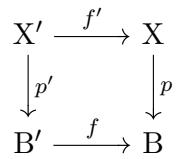
\includegraphics[keepaspectratio]{images/part001_dd3067cf.jpg}}

(E, II, p. 14). We shall then say, “Consider the square diagram (1),” or simply “the square (1),” instead of saying, “Consider the quadruple \(f,f^{\prime},p,p^{\prime}\) of continuous maps.” The square (1) is said to be commutative if the equality

\[
f \circ p ^ {\prime} = p \circ f ^ {\prime}
\]

is satisfied. In this case, one often endows B′, X, and X′ with the structures of B-spaces defined by the maps f, p, and \(f \circ p' = p \circ f'\) respectively; the maps \(p'\) and \(f'\) are then B-morphisms.

DEFINITION 4. --- We say that the square (1) is a Cartesian square of topological spaces (or, simply, that it is Cartesian) if it is commutative and if, for every topological space Y and every pair of continuous maps u: Y → B', v: Y → X such that f ∘ u = p ∘ v, there exists a unique continuous map w: Y → X' such that p' ∘ w = u and f' ∘ w = v.

For the square (1) to be Cartesian, it is necessary and sufficient that the square

(1')

\pandocbounded{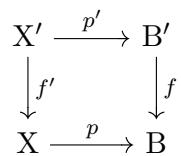
\includegraphics[keepaspectratio]{images/part001_f0fdde30.jpg}}

is Cartesian.

PROPOSITION 1. --- For the square (1) to be Cartesian, it is necessary and sufficient that it be commutative and that, for every B-space Y and every pair of B-morphisms \(u\colon Y \to B'\) , \(v\colon Y \to X\) there exists a unique B-morphism \(w\colon Y \to X'\) such that \(p' \circ w = u\) and \(f' \circ w = v\) .

Suppose that the square (1) is Cartesian. Let Y be a B-space and let \(u: Y \to B'\) and \(v: Y \to X\) be B-morphisms. The maps \(f \circ u\) and \(p \circ v\) are both equal to the projection of the B-space Y; the unique continuous map w such that \(p' \circ w = u\) and \(f' \circ w = v\) is then a B-morphism. This proves the necessity of the condition.

Conversely, suppose this condition is satisfied. Let Y be a topological space and let \(u \colon \mathrm{Y} \to \mathrm{B}'\) and \(v \colon \mathrm{Y} \to \mathrm{X}\) be continuous maps such that \(f \circ u = p \circ v\) . When Y is endowed with the B-space structure defined by \(f \circ u\) , \(u\) and \(v\) are B-morphisms. Every continuous map \(w \colon \mathrm{Y} \to \mathrm{X}'\) such that \(p' \circ w = u\) and \(f' \circ w = v\) is a B-morphism, so there exists exactly one such map.

PROPOSITION 2. --- Let B, B' and X be topological spaces and p: X → B, f: B' → B continuous maps.

\begin{enumerate}
\def\labelenumi{\alph{enumi})}
\tightlist
\item
  The square
\end{enumerate}

\[
\begin{array}{c} \mathrm{B} ^ {\prime} \times_ {\mathrm{B}} \mathrm{X} \xrightarrow {\mathrm{pr} _ {2}} \mathrm{X} \\ \Biggl \downarrow \mathrm{pr} _ {1} \\ \mathrm{B} ^ {\prime} \xrightarrow {f} \mathrm{B} \end{array}\tag{2}
\]

is a Cartesian square.

\begin{enumerate}
\def\labelenumi{\alph{enumi})}
\setcounter{enumi}{1}
\tightlist
\item
  For every commutative square
\end{enumerate}

\[
\begin{array}{c} \mathrm {X^ {\prime}} \xrightarrow {f ^ {\prime}} \mathrm{X} \\ \Big \downarrow_ {p ^ {\prime}} \\ \mathrm {B^ {\prime}} \xrightarrow {f} \mathrm{B} \end{array}\tag{3}
\]

there exists a unique continuous map \(h: X' \to B' \times_{B} X\) such that \(pr_{1} \circ h = p'\) and \(pr_{2} \circ h = f'\) .

\begin{enumerate}
\def\labelenumi{\alph{enumi})}
\setcounter{enumi}{2}
\tightlist
\item
  The commutative square (3) is Cartesian if and only if h is a homeomorphism.
\end{enumerate}

Assertion \(a\) ) follows from Proposition 1 and the universal property of the product of two B-spaces in the category of B-spaces (I, p. 3). Assertion \(b\) ) follows from it.

If the square (3) is Cartesian, there exists a unique continuous map \(h'\colon B'\times_{B}X\to X'\) such that \(f'\circ h' = pr_{2}\) and \(p'\circ h' = pr_{1}\) . We have \(f'\circ h'\circ h = f'\) and \(p'\circ h'\circ h = p'\) , whence \(h'\circ h = Id_{X'}\) since the square (3) is Cartesian. We have \(pr_{1}\circ h\circ h' = pr_{1}\) and \(pr_{2}\circ h\circ h' = pr_{2}\) , whence \(h\circ h' = Id_{B'\times_{B}X}\) since the square (2) is Cartesian. This proves that h is a homeomorphism.

Conversely, suppose that h is a homeomorphism; since square (2) is Cartesian, square (3) is also Cartesian.

The map \(h \colon \mathrm{X}' \to \mathrm{B}' \times_{\mathrm{B}} \mathrm{X}\) whose existence and uniqueness is asserted by part \(b)\) of the preceding proposition will be called canonical: it is the map denoted \((p', f')\) in I, p. 3.

PROPOSITION 3. --- Let

\[
\begin{array}{c} \mathrm {X^ {\prime}} \xrightarrow {f ^ {\prime}} \mathrm{X} \\ \Big \downarrow_ {p ^ {\prime}} \\ \mathrm {B^ {\prime}} \xrightarrow {f} \mathrm{B} \end{array}
\]

a Cartesian square. For any continuous section s of \(p'\) , the map \(f'\circ s\) is a continuous lift of f to X. The map \(s\mapsto f'\circ s\) is a bijection from \(\mathcal{C}_{\mathrm{B}'}(\mathrm{B}';\mathrm{X}')\) onto \(\mathcal{C}_{\mathrm{B}}(\mathrm{B}';\mathrm{X})\) .

If \(s \colon B' \to X'\) is a continuous section of \(p'\) , we have \(p \circ f' \circ s = f \circ p' \circ s = f\) , which proves that \(f' \circ s\) is a continuous lifting of \(f\) to X, i.e., a B-morphism from \(B'\) into X. Conversely, let \(g \colon B' \to X\) be a B-morphism. We have \(f \circ \mathrm{Id}_{\mathrm{B}'} = p \circ g\) ; there therefore exists, by definition of a Cartesian square, a unique continuous map \(s \colon B' \to X'\) such that \(p' \circ s = \mathrm{Id}_{\mathrm{B}'}\) and \(f' \circ s = g\) , whence the proposition.

\subsection{Cartesian squares constructed by passing to subspaces}

PROPOSITION 4. --- Let

\[
\begin{array}{c} \mathrm {X^ {\prime}} \xrightarrow {f ^ {\prime}} \mathrm{X} \\ \Big \downarrow_ {p ^ {\prime}} \\ \mathrm {B^ {\prime}} \xrightarrow {f} \mathrm{B} \end{array}\tag{4}
\]

a Cartesian square and let \(B_{0}\) , \(B_{0}^{\prime}\) , \(X_{0}\) be subspaces of B, \(B^{\prime}\) and X, respectively. Suppose we have \(f(B_{0}^{\prime}) \subset B_{0}\) , \(p(X_{0}) \subset B_{0}\) and let us set \(X_{0}^{\prime} = \overline{p'}^{1}(B_{0}^{\prime}) \cap \overline{f'}^{1}(X_{0})\) . Then, the square

\[
\begin{array}{c} \mathrm{X} _ {0} ^ {\prime} \xrightarrow {f _ {0} ^ {\prime}} \mathrm{X} _ {0} \\ \Biggl \downarrow p _ {0} ^ {\prime} \\ \mathrm{B} _ {0} ^ {\prime} \xrightarrow {f _ {0}} \mathrm{B} _ {0} \end{array}\tag{4'}
\]

(where the maps \(f_0\) , \(f_0'\) , \(p_0\) , \(p_0'\) are deduced from \(f\) , \(f'\) , \(p\) , \(p'\) respectively by passing to subsets) is Cartesian.

Consider the canonical map \(h \colon X' \to B' \times_B X\) deduced from the commutative diagram (4). Since square (4) is Cartesian, \(h\) is a homeomorphism. By construction, we have \(X_0' = h^{-1}(B_0' \times_{B_0} X_0)\) and the mapping \(h_0 \colon X_0' \to B_0' \times_{B_0} X_0\) deduced from the commutative diagram ( \(4'\) ) is deduced from \(h\) by passing to subsets. It is therefore a homeomorphism, and the square ( \(4'\) ) is Cartesian (prop. 2).

COROLLARY. --- Let

\pandocbounded{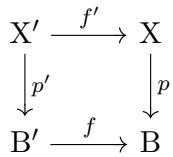
\includegraphics[keepaspectratio]{images/part001_2907af81.jpg}}

a Cartesian square.

\begin{enumerate}
\def\labelenumi{\alph{enumi})}
\item
  For every point \(b'\) of \(B'\) , the map \(f'\) induces a homeomorphism of the fiber \(X_{b'}'\) of \(p'\) onto the fiber \(X_{f(b')}\) of \(p\) .
\item
  If the map p is injective (resp. surjective, resp. bijective), then so is \(p'\) .
\end{enumerate}

Let \(b'\) be a point of B'. Set \(b = f(b')\) . For all \(x' \in X_{b'}'\) , we have \(p(f'(x')) = f(p'(x')) = f(b') = b\) , whence \(f'(x') \in X_b\) . This proves that one has \(X_{b'}' \subset \overline{f'}^{1}(X_b)\) . In Proposition 4, take \(B_0 = \{b\}\) , \(B_0' = \{b'\}\) and \(X_0 = X_b\) ; we then have \(X_0' = X_{b'}'\) , whence the assertion \(a\) ).

For the map p to be injective (resp. surjective, resp. bijective), it is necessary and sufficient that the cardinality of each of its fibers be at most (resp. at least, resp. equal to) 1. Assertion b) follows from this.

Example. --- Let \((X,p)\) be a B-space and A a subspace of B. The square

\[
\begin{array}{c} \overline {{p}} ^ {1} (\mathrm{A}) \xrightarrow {j} \mathrm{X} \\ \Biggl \downarrow p _ {\mathrm{A}} \\ \mathrm{A} \xrightarrow {i} \mathrm{B} \end{array}\tag{5}
\]

(where i and j are the canonical injections) is cartesian.

In particular, if A and A' are subspaces of the topological space B, the square

\begin{enumerate}
\def\labelenumi{(\arabic{enumi})}
\setcounter{enumi}{5}
\tightlist
\item
\end{enumerate}

\pandocbounded{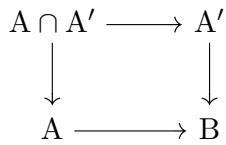
\includegraphics[keepaspectratio]{images/part001_a4278a10.jpg}}

(where the arrows are the canonical injections) is cartesian.

\subsection{Cartesian squares constructed by products, fibered products, and sums}

PROPOSITION 5. --- Let I be a set and, for every \(i \in I\) , let

\[
\begin{array}{c} \mathrm{X} _ {i} ^ {\prime} \xrightarrow {f _ {i} ^ {\prime}} \mathrm{X} _ {i} \\ \Big \downarrow p _ {i} ^ {\prime} \\ \mathrm{B} _ {i} ^ {\prime} \xrightarrow {f _ {i}} \mathrm{B} _ {i} \end{array}\tag{7}
\]

a cartesian square. The square

\[
\begin{array}{c} \prod_ {i \in \mathrm{I}} \mathrm{X} _ {i} ^ {\prime} \xrightarrow {f ^ {\prime}} \prod_ {i \in \mathrm{I}} \mathrm{X} _ {i} \\ \Biggl \downarrow^ {p ^ {\prime}} \qquad \qquad \qquad \qquad \Biggl \downarrow^ {p} \\ \prod_ {i \in \mathrm{I}} \mathrm{B} _ {i} ^ {\prime} \xrightarrow {f} \prod_ {i \in \mathrm{I}} \mathrm{B} _ {i} \end{array}\tag{ (7') }
\]

\((\text{where } f, f', p, p' \text{ are the extensions of the families } (f_i), (f'_i), (p_i), (p'_i) \text{ to products}) \text{ is Cartesian.}\)

Let Y be a topological space, and let \(u \colon \mathrm{Y} \to \prod_{i} \mathrm{B}_{i}'\) and \(v \colon \mathrm{Y} \to \prod_{i} \mathrm{X}_{i}\) be continuous maps such that \(f \circ u = p \circ v\) . For \(i \in \mathrm{I}\) , set \(u_{i} = \mathrm{pr}_{i} \circ u\) and \(v_{i} = \mathrm{pr}_{i} \circ v\) ; we have \(f_{i} \circ u_{i} = p_{i} \circ v_{i}\) and there exists a unique continuous map \(w_{i} \colon \mathrm{Y} \to \mathrm{X}_{i}'\) such that \(p_{i}' \circ w_{i} = u_{i}\) and \(f_{i}' \circ w_{i} = v_{i}\) . Then, the map \(w = (w_{i})\) is a continuous map from Y into \(\prod_{i} \mathrm{X}_{i}'\) such that \(p' \circ w = u\) and \(f' \circ w = v\) and it is the only one having these properties.

COROLLARY 1. --- Let X be a B-space, let p be its projection, and let F be a topological space. The square

\[
\begin{array}{c} \mathrm{X} \times \mathrm{F} \xrightarrow {\operatorname{pr} _ {1}} \mathrm{X} \\ \Biggl \downarrow p \times \mathrm{Id} _ {\mathrm{F}} \\ \mathrm{B} \times \mathrm{F} \xrightarrow {\operatorname{pr} _ {1}} \mathrm{B} \end{array}\tag{8}
\]

is Cartesian.

Let P be a topological space reduced to a point. Corollary 1 follows from Prop. 5 applied to the Cartesian squares

\[
\begin{array}{l} \mathrm{X} \xrightarrow {\mathrm{Id} _ {\mathrm{X}}} \mathrm{X} \\ \Big \downarrow_ {p} \qquad \Big \downarrow_ {p} \\ \mathrm{B} \xrightarrow {\mathrm{Id} _ {\mathrm{B}}} \mathrm{B} \end{array} \qquad \text {and} \qquad \begin{array}{l} \mathrm{F} \longrightarrow \mathrm{P} \\ \Big \downarrow_ {\mathrm{Id} _ {\mathrm{F}}} \qquad \Big \downarrow_ {\mathrm{Id} _ {\mathrm{P}}} \\ \mathrm{F} \longrightarrow \mathrm{P}. \end{array}
\]

Let B and B' be topological spaces, and let \(f: B' \to B\) be a continuous map. Let I be a set and, for every \(i \in I\) , let \(X_i\) be a B-space, \(X'_i\) be a B'-space, and \(f'_i: X'_i \to X_i\) be a continuous map such that the square

\[
\begin{array}{c} \mathrm{X} _ {i} ^ {\prime} \xrightarrow {f _ {i} ^ {\prime}} \mathrm{X} _ {i} \\ \Big \downarrow \\ \mathrm{B} ^ {\prime} \xrightarrow {f} \mathrm{B} \end{array}\tag{9}
\]

is commutative. There exists a unique continuous map

\[
f ^ {\prime} \colon \prod_ {i \in \mathrm{I}} \mathrm{X} _ {i} ^ {\prime} \to \prod_ {i \in \mathrm{I}} \mathrm{X} _ {i}
\]

such that \(pr_{i} \circ f' = f_{i}' \circ pr_{i}\) for all \(i \in I\) and such that the square

\[
\begin{array}{c} \prod_ {i \in I} X _ {i} ^ {\prime} \xrightarrow {f ^ {\prime}} \prod_ {i \in I} X _ {i} \\ \Big \downarrow \qquad \qquad \qquad \qquad \Big \downarrow \\ B ^ {\prime} \xrightarrow {f} B \end{array}\tag{ (9') }
\]

is commutative (this last condition following from the others if I ≠ ∅): it is the map deduced from the map

\[
f \times \prod_ {i \in \mathrm{I}} f _ {i} ^ {\prime} \colon \mathrm{B} ^ {\prime} \times \prod_ {i \in \mathrm{I}} \mathrm{X} _ {i} ^ {\prime} \to \mathrm{B} \times \prod_ {i \in \mathrm{I}} \mathrm{X} _ {i}
\]

by passing to subsets. With these notations:

COROLLARY 2. --- If the square (9) is Cartesian for every \(i \in I\) , then the square ( \(9'\) ) is Cartesian.

From prop. 5 one deduces a Cartesian square

\[
\begin{array}{c} \mathrm{B} ^ {\prime} \times \prod_ {i} \mathrm{X} _ {i} ^ {\prime} \xrightarrow {\operatorname{Id} _ {\mathrm{B}} \times \prod_ {i} f _ {i} ^ {\prime}} \mathrm{B} \times \prod_ {i} \mathrm{X} _ {i} \\ \Biggl \downarrow \\ \mathrm{B} ^ {\prime} \times (\mathrm{B} ^ {\prime}) ^ {\mathrm{I}} \xrightarrow {f \times \prod_ {i} f} \mathrm{B} \times \mathrm{B} ^ {\mathrm{I}}  . \end{array}
\]

Denote by \(\Delta_{\mathrm{B}^{\prime}}\) and \(\Delta_{\mathrm{B}}\) the diagonals of \(\mathrm{B}^{\prime}\times (\mathrm{B}^{\prime})^{\mathrm{I}}\) and \(\mathrm{B}\times \mathrm{B}^{\mathrm{I}}\) . The diagram

\[
\begin{array}{c} \prod_ {i \in \mathrm{I}} X _ {i} ^ {\prime} \xrightarrow {f ^ {\prime}} \prod_ {i \in \mathrm{I}} X _ {i} \\ \Big \downarrow \qquad \qquad \qquad \Big \downarrow \\ \Delta_ {\mathrm{B} ^ {\prime}} \xrightarrow {} \Delta_ {\mathrm{B}} \end{array}
\]

deduced from the preceding one by passing to subspaces is Cartesian (I, p. 9, prop. 4). It is identified with diagram (9').

Example 1. --- Let

\[
\begin{array}{c} \mathrm {X^ {\prime}} \xrightarrow {f ^ {\prime}} \mathrm{X} \\ \Big \downarrow_ {p ^ {\prime}} \\ \mathrm {B^ {\prime}} \xrightarrow {f} \mathrm{B} \end{array}
\]

a Cartesian square. Then Corollary 2 provides a Cartesian square

\[
\begin{array}{c} \mathrm {X^ {\prime} \times_ {B^ {\prime}} X^ {\prime}} \xrightarrow {\varphi} \mathrm {X\times_ {B} X} \\ \Big \downarrow \\ \mathrm {B^ {\prime} \xrightarrow {f} B}. \end{array}
\]

We have the relation \(\overline{\varphi}^{1}(\Delta_{\mathrm{X}}) = \Delta_{\mathrm{X}^{\prime}}\) . Indeed, by Proposition 2 of I, p. 8, it suffices to consider the case where \(\mathrm{X}' = \mathrm{B}' \times_{\mathrm{B}} \mathrm{X}\) . Let then \(((b,x),(b,x'))\) be an element of \(X^{\prime} \times_{B^{\prime}} X^{\prime}\) with \(b \in B^{\prime}\) and \(x, x^{\prime} \in X\) . This element belongs to \(\overline{\varphi}^{1}(\Delta_{\mathrm{X}})\) if and only if \(x = x^{\prime}\) .

PROPOSITION 6. --- Let I be a set and, for every \(i \in I\) , let

\[
\begin{array}{c} \mathrm{X} _ {i} ^ {\prime} \xrightarrow {f _ {i} ^ {\prime}} \mathrm{X} \\ \Biggl \downarrow p _ {i} ^ {\prime} \\ \mathrm{B} _ {i} ^ {\prime} \xrightarrow {f _ {i}} \mathrm{B} \end{array}\tag{10}
\]

a Cartesian square. Let X' and B' be the sum spaces of the families \((X'_i)\) and \((B'_i)\), respectively. Let f: B' → B, f': X' → X, and p': X' → B' be the maps induced from the families \((f_i)\), \((f'_i)\), and \((p'_i)\), respectively. The square

\((10')\)

\pandocbounded{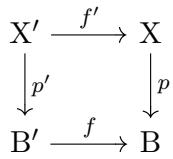
\includegraphics[keepaspectratio]{images/part001_48571453.jpg}}

is Cartesian.

The maps \(f\) , \(f'\) , and \(p'\) are continuous. The commutativity of the square \((10')\) follows from its definition. Let \(h_i\) denote the canonical homeomorphism from \(\mathrm{X}_i'\) onto \(\mathrm{B}_i' \times_{\mathrm{B}} \mathrm{X}\) (I, p. 8, Proposition 2) and let \(h: \mathrm{X}' \to \mathrm{B}' \times_{\mathrm{B}} \mathrm{X}\) be the canonical map (loc. cit.). We have \(h = h'' \circ h'\) , where \(h': \mathrm{X}' \to \coprod (\mathrm{B}_i' \times_{\mathrm{B}} \mathrm{X})\) is the homeomorphism induced by the \(h_i\) and \(h'': \coprod (\mathrm{B}_i' \times_{\mathrm{B}} \mathrm{X}) \to (\coprod \mathrm{B}_i') \times_{\mathrm{B}} \mathrm{X}\) is the one defined in Example 5 of I, p. 4. We conclude by Proposition 2 of I, p. 8.

Example 2. --- Let \((X,p)\) be a B-space and let \((\mathrm{A}_{k})_{k\in\mathrm{K}}\) be a family of subspaces of B. Let A be the sum space of the family \((\mathrm{A}_{k})_{k\in\mathrm{K}}\) and let Y be the sum space of the family \((\overline{p}^{1}(\mathrm{A}_{k}))_{k\in\mathrm{K}}\) ; let us denote by \(i: A \to B\) , \(j: Y \to X\) , and \(p': Y \to A\) the maps induced by the canonical injections of \(A_{k}\) into B, the canonical injections of \(\overline{p}^{1}(\mathrm{A}_{k})\) into X, and the maps \(p_{\mathrm{A}_{k}}: \overline{p}^{1}(\mathrm{A}_{k}) \to \mathrm{A}_{k}\) , for \(k \in K\) . The square

\[
\begin{array}{c} \mathrm{Y} \xrightarrow {j} \mathrm{X} \\ \Biggl \downarrow p ^ {\prime} \\ \mathrm{A} \xrightarrow {i} \mathrm{B} \end{array}\tag{11}
\]

is Cartesian; this follows from the example in I, p. 10 and from Prop. 6.

\subsection{Composition of Cartesian squares}

PROPOSITION 7. --- Let

\[
\begin{array}{c} \mathrm {X^ {\prime\prime}} \xrightarrow {g ^ {\prime}} \mathrm {X^ {\prime}} \\ \Big \downarrow_ {p ^ {\prime \prime}} \\ \mathrm {B^ {\prime\prime}} \xrightarrow {g} \mathrm {B^ {\prime}} \end{array}\tag{12}
\]

and

\begin{enumerate}
\def\labelenumi{(\arabic{enumi})}
\setcounter{enumi}{12}
\tightlist
\item
\end{enumerate}

\pandocbounded{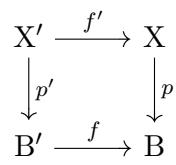
\includegraphics[keepaspectratio]{images/part001_4552bd62.jpg}}

of commutative squares; consider the square

\begin{enumerate}
\def\labelenumi{(\arabic{enumi})}
\setcounter{enumi}{13}
\tightlist
\item
\end{enumerate}

\pandocbounded{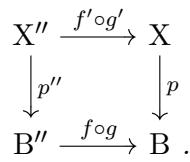
\includegraphics[keepaspectratio]{images/part001_1603e4c4.jpg}}

It is commutative. If squares (12) and (13) are Cartesian, then so is square (14). If squares (13) and (14) are Cartesian, then so is square (12).

Square (14) is commutative, since we have \(p \circ f' \circ g' = f \circ p' \circ g' = f \circ g \circ p''\) . Denote by \(h' : X'' \to B'' \times_{B'} X'\) , \(h : X' \to B' \times_{B} X\) and \(h'' : X'' \to B'' \times_{B} X\) the canonical continuous maps deduced from the commutative squares (12), (13), and (14). Moreover, denote

\[
j \colon \mathrm{B} ^ {\prime \prime} \times_ {\mathrm{B}} \mathrm{X} \rightarrow \mathrm{B} ^ {\prime \prime} \times_ {\mathrm{B} ^ {\prime}} (\mathrm{B} ^ {\prime} \times_ {\mathrm{B}} \mathrm{X})
\]

the continuous map that sends \((b'', x)\) to \((b'', g(b''), x)\) . It is a homeomorphism and one has \(j \circ h'' = (\mathrm{Id}_{\mathrm{B}''} \times_{\mathrm{B}} h) \circ h'\) .

Suppose that square (13) is Cartesian. Then h is a homeomorphism (I, p. 8, prop 2), so the map \(Id_{B''} \times_{B} h\) is a homeomorphism, and \(h''\) is a homeomorphism if and only if \(h'\) is one. This means that square (12) is Cartesian if and only if square (14) is Cartesian (loc. cit.).

With the notation of Proposition 7, one sometimes says that square (14) is the composite square of squares (13) and (12). The first assertion expresses that the composite of two Cartesian squares is Cartesian. In particular, the B''-spaces \(g^{*}(f^{*}(\mathrm{X}))\) and \((f \circ g)^{*}(\mathrm{X})\) are isomorphic.

\pandocbounded{
\includegraphics[keepaspectratio]{images/part001_52f28a70.jpg}}

Remarks. --- 1) It can happen that the squares (12) and (14) are Cartesian without the square (13) being so (I, p. 139, exerc. 2).

\begin{enumerate}
\def\labelenumi{\arabic{enumi})}
\setcounter{enumi}{1}
\tightlist
\item
  Let \(p \colon \mathrm{X} \to \mathrm{B}\) and \(f \colon \mathrm{B}' \to \mathrm{B}\) be continuous maps. The map \(g \colon \mathrm{B}' \to \mathrm{B}' \times \mathrm{B}\) defined by \(g(b') = (b', f(b'))\) is a homeomorphism from \(\mathrm{B}'\) onto the graph \(\mathrm{G}\) of the map \(f\) (TG, I, p. 25, cor. 2), and the fibered product \(\mathrm{B}' \times_{\mathrm{B}} \mathrm{X}\) is identified (I, p. 6) with the subspace of \(\mathrm{B}' \times \mathrm{X}\) that is the inverse image of \(\mathrm{G}\) under the map \(\mathrm{Id}_{\mathrm{B}'} \times p \colon \mathrm{B}' \times \mathrm{X} \to \mathrm{B}' \times \mathrm{B}\) . By the example of I, p. 10 and Corollary 1 of Proposition 5 (I, p. 11), the squares
\end{enumerate}

\[
\begin{array}{c c} \mathrm {B^ {\prime}} \times_ {\mathrm{B}} \mathrm{X} \xrightarrow {i} \mathrm {B^ {\prime}} \times \mathrm{X} & \mathrm {B^ {\prime}} \times \mathrm{X} \xrightarrow {\mathrm{pr} _ {2}} \mathrm{X} \\ \Biggl \downarrow \mathrm{pr} _ {1} & \Biggl \downarrow \mathrm{Id} _ {\mathrm {B^ {\prime}}} \times p \\ \mathrm {B^ {\prime}} \xrightarrow {g} \mathrm {B^ {\prime}} \times \mathrm{B} & \text {et} \end{array} \qquad \qquad \begin{array}{c c} \mathrm {B ^ {\prime}} \times \mathrm{X} \xrightarrow {\mathrm{pr} _ {2}} \mathrm{X} \\ \Biggl \downarrow \mathrm{Id} _ {\mathrm {B^ {\prime}}} \times p & \Biggl \downarrow p \\ \mathrm {B^ {\prime}} \times \mathrm{B} \xrightarrow {\mathrm{pr} _ {2}} \mathrm{B} & \end{array}
\]

(where i denotes the canonical injection) are Cartesian, and the Cartesian square

\[
\begin{array}{c} \mathrm{B} ^ {\prime} \times_ {\mathrm{B}} \mathrm{X} \xrightarrow {\mathrm{pr} _ {2}} \mathrm{X} \\ \Big \downarrow \mathrm{pr} _ {1} \\ \mathrm{B} ^ {\prime} \xrightarrow {f} \mathrm{B} \end{array}
\]

is their composite. In other words, every Cartesian square is identified with the composite square of a Cartesian square obtained by taking a product (I, p. 11, Corollary 1 of Proposition 5, square (8)) and a Cartesian square obtained by passing to subspaces (I, p. 10, example, square (5)).

\begin{enumerate}
\def\labelenumi{\arabic{enumi})}
\setcounter{enumi}{2}
\tightlist
\item
  Let
\end{enumerate}

\[
\begin{array}{c} \mathrm{X} _ {1} \xrightarrow {g _ {1}} \mathrm{X} \\ \Biggl \downarrow p _ {1} \\ \mathrm{B} _ {1} \xrightarrow {f _ {1}} \mathrm{B} \end{array}\tag{15}
\]

and

\[
\begin{array}{c} \mathrm{X} _ {2} \xrightarrow {g _ {2}} \mathrm{X} \\ \Biggl \downarrow p _ {2} \\ \mathrm{B} _ {2} \xrightarrow {f _ {2}} \mathrm{B} \end{array}\tag{16}
\]

  Let

\[
\begin{array}{c} \mathrm{X} _ {1} \times_ {\mathrm{X}} \mathrm{X} _ {2} \xrightarrow {g} \mathrm{X} \\ \Big \downarrow^ {p ^ {\prime}} \\ \mathrm{B} _ {1} \times_ {\mathrm{B}} \mathrm{B} _ {2} \xrightarrow {f} \mathrm{B} \end{array}\tag{17}
\]

where \(f\) (resp. \(g\) ) is the map that defines the structure of a B-space (resp. of an X-space) on the fibered product \(\mathrm{B}_{1} \times_{\mathrm{B}} \mathrm{B}_{2}\) (resp. on the fibered product \(\mathrm{X}_{1} \times_{\mathrm{X}} \mathrm{X}_{2}\) ) and where \(p'\) is the map induced by \(p_{1} \times p_{2}\) by passing to subspaces. It is Cartesian (I, p. 13, Corollary 2 of Proposition 5).

Now consider the following two commutative squares:

\[
\begin{array}{c c} \mathrm{X} _ {1} \times_ {\mathrm{X}} \mathrm{X} _ {2} \xrightarrow {\operatorname{pr} _ {1}} \mathrm{X} _ {1} & \mathrm{X} _ {1} \times_ {\mathrm{X}} \mathrm{X} _ {2} \xrightarrow {\operatorname{pr} _ {2}} \mathrm{X} _ {2} \\ \Biggl \downarrow p ^ {\prime} & \text {and} \\ \mathrm{B} _ {1} \times_ {\mathrm{B}} \mathrm{B} _ {2} \xrightarrow {\operatorname{pr} _ {1}} \mathrm{B} _ {1} & \mathrm{(19)} \\ & \mathrm{B} _ {1} \times_ {\mathrm{B}} \mathrm{B} _ {2} \xrightarrow {\operatorname{pr} _ {2}} \mathrm{B} _ {2}. \end{array}\tag{18}
\]

Square (17) is composed of squares (15) and (18), as well as squares (16) and (19). By prop. 7, squares (18) and (19) are Cartesian.

\subsection{Strict maps}

PROPOSITION 8. --- Let

\[
\begin{array}{c} \mathrm {X^ {\prime}} \xrightarrow {f ^ {\prime}} \mathrm{X} \\ \Big \downarrow_ {p ^ {\prime}} \\ \mathrm {B^ {\prime}} \xrightarrow {f} \mathrm{B} \end{array}
\]

a Cartesian square. If the map p is open (resp. is proper, resp. has a continuous section in a neighborhood of every point), then so is \(p'\).

By Remark 2, I, p. 16, it suffices to prove the proposition for Cartesian squares of the following type:

\[
\begin{array}{c c} \overline {{p}} ^ {1} (\mathrm {A}) \xrightarrow {j} \mathrm{X} & \mathrm {A} \times \mathrm{F} \xrightarrow {i} \mathrm{X} \times \mathrm{F} \\ \Big \downarrow_ {p _ {\mathrm {A}}} & \Big \downarrow_ {p \times \mathrm {Id}_{\mathrm {F}}} \\ \mathrm {A} & \xrightarrow {i} \mathrm {B} \end{array} \quad\text {and} \quad \begin{array}{c} \mathrm {X} \times \mathrm {F} \xrightarrow {j} \mathrm {X} \\ \Big \downarrow_ {p \times \mathrm {Id}_{\mathrm {F}}} \\ \mathrm {B} \times \mathrm {F} \xrightarrow {i} \mathrm {B} \end{array}
\]

where F is a topological space, A is a subspace of B, and i and j are the canonical injections. If the map p is open, the maps \(p_{A}\) and \(p \times Id_{F}\) are open (TG, I, p. 30, prop. 2 and TG, I, p. 34, prop. 8). If the map p is proper, then the maps \(p_{A}\) and \(p \times Id_{F}\) are proper (TG, I, p. 72, prop. 3 and TG, I, p. 72, def. 1). If U is an open subset of B and \(s\colon\mathrm{U}\to\mathrm{X}\) is a continuous section of p on U, the map \(s\mid(\mathrm{A}\cap\mathrm{U})\) is a continuous section of \(p_{\mathrm{A}}\) onto \(\mathrm{A}\cap\mathrm{U}\), and the map \(s\times\mathrm{Id}_{\mathrm{F}}\) is a continuous section of \(p\times\mathrm{Id}_{\mathrm{F}}\) onto \(\mathrm{U}\times\mathrm{F}\).

Remark 1. --- With the notation of Proposition 8, if \(p\) is a closed map, it is not necessarily the case that \(p'\) is closed (cf. TG, I, p. 32, prop. 3). However, if \(p\) is a map with a continuous section, \(p'\) also has a continuous section.

DEFINITION 5. --- Let X and Y be topological spaces and let f: X → Y be a map. Let R be the equivalence relation associated with f and

\[
\mathrm{X} \rightarrow \mathrm{X} / \mathrm{R} \xrightarrow {g} f (\mathrm{X}) \rightarrow \mathrm{Y}
\]

the canonical decomposition of \(f\) (E, II, p. 44). We say that the map \(f\) is strict if \(g\) is a homeomorphism, when \(X/R\) is equipped with the quotient topology and \(f(X)\) is equipped with the topology induced by that of \(Y\).

A strict map is continuous.

Recall (TG, I, p. 22, prop. 8) that for a map \(f\) to be strict, it is necessary and sufficient that \(f\) be continuous and that, for every subset \(A\) of \(X\) which is open (resp. closed) and saturated, \(f(A)\) be open (resp. closed) in \(f(X)\).

Examples. --- 1) The composition of two strict maps is not necessarily strict. Indeed, every continuous map \(f \colon X \to Y\) is the composite of the map \(\mathrm{pr}_2 \colon X \times Y \to Y\) and the map \(x \mapsto (x, f(x))\) from \(X\) into \(X \times Y\), both of which are strict (TG, I, p. 26, prop. 5 and TG, I, p. 25, cor. 2). On the other hand, the composite of two strict and injective (resp. surjective) maps is a strict map.

\begin{enumerate}
\def\labelenumi{\arabic{enumi})}
\setcounter{enumi}{1}
\item
  A continuous map that is open, or closed, or has a continuous section, is strict. This follows from Prop. 3 of TG, I, p. 32 and Prop. 9 of TG, I, p. 22.
\item
  For a continuous homomorphism from one topological group to another to be a strict morphism (TG, III, p. 16, def. 1), it is necessary and sufficient that it be a strict map in the sense of Definition 5.
\end{enumerate}

PROPOSITION 9. --- Let X, Y, and Z be topological spaces. Let \(f\colon X \to Y\) be a continuous surjective map and \(g\colon Y \to Z\) a map.

\begin{enumerate}
\def\labelenumi{\alph{enumi})}
\item
If f is strict and if g∘f is continuous, then the map g is continuous.
\item
If g is continuous and if g∘f is strict, then g is strict.
\item
If f and g \(\circ\) f are strict, then g is strict.
\end{enumerate}

Let us prove assertion a). Let R denote the relation associated with f in X; by hypothesis, the map from X/R onto Y induced by f by passing to the quotient is a homeomorphism. The first assertion then follows from Proposition 6 of I, p. 21.

Let us prove b). Let B be a closed saturated subset of Y for the relation defined by g, and let \(A = f^{-1}(B)\). Since f is continuous, A is closed in X, and A is saturated for the equivalence relation defined by \(g \circ f\). Since \(g \circ f\) is strict and f is surjective, \(g(B) = g \circ f(A)\) is then closed in Z. The continuous map g is therefore strict.

Assertion c) follows immediately from assertions a) and b).

PROPOSITION 10. --- Let X be a topological space and let R be an equivalence relation on X. Let Y be a locally compact topological space. Let S be the equivalence relation on X × Y which is the product of the equivalence relation R on X and the equality relation on Y. The canonical bijection (X × Y)/S → (X/R) × Y is a homeomorphism.

Recall that if U and V are topological spaces, \(\mathcal{C}_{c}(\mathrm{U};\mathrm{V})\) denotes the set of continuous maps from U to V, endowed with the compact-open topology (TG, X, p. 26, def. 1).

Let \(p \colon \mathrm{X} \to \mathrm{X} / \mathrm{R}\) and \(q \colon \mathrm{X} \times \mathrm{Y} \to (\mathrm{X} \times \mathrm{Y}) / \mathrm{S}\) be the canonical surjections. Let \(g \colon (\mathrm{X} \times \mathrm{Y}) / \mathrm{S} \to (\mathrm{X} / \mathrm{R}) \times \mathrm{Y}\) be the canonical bijection. It is continuous; let us denote its inverse by \(h\) and prove that it is continuous.

The map \(i\colon X \to \mathcal{C}_{c}(Y;X \times Y)\) such that, for every \(x \in X\), \(i(x)\) is the map defined by \(y \mapsto (x,y)\), is continuous (TG, X, p. 28, Theorem 3). The map \(\widetilde{q}\colon \mathcal{C}_{c}(Y;X \times Y) \to \mathcal{C}_{c}(Y;(X \times Y)/S)\), which associates to a continuous map \(\varphi\) the map \(q \circ \varphi\), is continuous (TG, X, p. 29, Proposition 9). Consequently, the map \(\widetilde{q} \circ i\colon X \to \mathcal{C}_{c}(Y;(X \times Y)/S)\) is continuous. It is compatible with the equivalence relation R; the unique map \(j\colon X/R \to \mathcal{C}_{c}(Y;(X \times Y)/S)\) such that \(j \circ p = \widetilde{q} \circ i\) is therefore continuous. We have \(h(\xi,y) = j(\xi)(y)\) for every pair \((\xi,y) \in (X/R) \times Y\). Since Y is locally compact, it follows from TG, X, p. 28, Theorem 3 that \(h\) is continuous.

The conclusion of Proposition 10 is no longer necessarily valid if Y is not locally compact (TG, I, p. 96, exerc. 6).

COROLLARY. --- Let X and Y be topological spaces and let \(f: X \to Y\) be a continuous map. Let T be a locally compact topological space. If the map f is strict, then so is the map \(f \times Id_{T}\) from \(X \times T\) into \(Y \times T\).

\subsection{Universally strict maps}

Let

\[
\begin{array}{c} \mathrm {X^ {\prime}} \xrightarrow {f ^ {\prime}} \mathrm{X} \\ \Big \downarrow_ {p ^ {\prime}} \\ \mathrm {B^ {\prime}} \xrightarrow {f} \mathrm{B} \end{array}
\]

a Cartesian square, where p is strict. The map \(p'\) is not necessarily strict (cf. Remark 1). However, if A is open (resp. closed) in B, the map \(p_A: \overline{p}^{1}(A) \to A\) is strict.

DEFINITION 6. --- Let p: X → B be a map. We say that p is universally strict if, for every Cartesian square

\pandocbounded{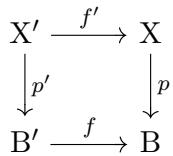
\includegraphics[keepaspectratio]{images/part001_50963eb1.jpg}}

the map p' is strict.

A universally strict map is strict. With the notation of Definition 6, if \(p\) is universally strict, then \(p'\) is universally strict as well. This follows immediately from the definition.

COROLLARY. --- An open map, a proper map, and a map having a continuous local section are universally strict.

Example. --- Let B be a topological space and \((\mathrm{A}_{i})_{i\in\mathrm{I}}\) a covering of B; we denote by A the sum space of the family \((\mathrm{A}_{i})_{i\in\mathrm{I}}\), and \(p: A \to B\) the canonical map. The map p is universally strict under each of the following two hypotheses:

\begin{enumerate}
\def\labelenumi{(\roman{enumi})}
\item
  For every point \(b \in B\) , there exists \(i \in I\) such that b is an interior point of \(A_{i}\) ;
\item
  The family \((A_{i})\) is locally finite and the \(A_{i}\) are closed subsets of B.
\end{enumerate}

Under hypothesis (i), the map p has a continuous section in a neighborhood of every point. Under hypothesis (ii), the map p is proper by definition of the sum space (resp. by TG, I, p. 6, prop. 4 and TG, I, p. 75, th. 1). It is therefore universally strict.

Remark. --- A closed map is not necessarily universally strict (cf. TG, I, p. 96, exerc. 6).

PROPOSITION 11. --- Let

\pandocbounded{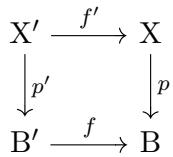
\includegraphics[keepaspectratio]{images/part001_02f1b349.jpg}}

a Cartesian square.

\begin{enumerate}
\def\labelenumi{\alph{enumi})}
\item
Suppose f is strict and surjective. Then, if p' is open (resp. closed, resp. proper), so is p.
\item
Suppose f is closed and surjective. If p' is strict, then p is strict.
\item
Suppose f is universally strict. If p' is universally strict, then p is universally strict.
\end{enumerate}

Note first that for every subset A of X, we have

\[
p ^ {\prime} ((\stackrel {- 1} {f ^ {\prime}}) (\mathrm{A})) = \stackrel {- 1} {f} (p (\mathrm{A})).\tag{20}
\]

Indeed, if \(x' \in (f')^{-1}(\mathrm{A})\), then \(f(p'(x')) = p \circ f'(x') \in p(\mathrm{A})\). Conversely, if \(b' \in f^{-1}(p(\mathrm{A}))\), let \(x \in A\) be such that \(f(b') = p(x)\). By definition of a Cartesian square, there exists a unique \(x' \in X'\) such that \(f'(x') = x\) and \(p'(x') = b'\), so that \(b' \in p'((f')^{-1}(\mathrm{A}))\).

Suppose that f is an open map and \(p'\) is a strict map.

The set \((f')^{-1}(\mathrm{A})\) is open (resp. closed) in \(\mathrm{X}'\). Consequently, the set \(p'((f')^{-1}(\mathrm{A}))\) is open (resp. closed) in \(\mathrm{B}'\). By relation (20), it is also saturated for the equivalence relation defined by \(f\). Since the map \(f\) is assumed to be surjective, we then have \(p(\mathrm{A}) = f(p'((f')^{-1}(\mathrm{A})))\), and since it is strict, the set \(p(\mathrm{A})\) is open (resp. closed) in B. The map \(p\) is therefore open (resp. closed).

For a continuous map to be proper, it is necessary and sufficient that it be closed and that its fibers be quasi-compact (TG, I, p. 75, th. 1). If the map \(p'\) is proper, the map \(p\) is closed by what precedes. Let us study its fibers: if \(b \in B\), let \(b' \in B'\) be such that \(f(b') = b\). By the corollary of I, p. 10, the map \(f'\) induces a homeomorphism \(X_{b'}' \to X_b\). Since \(p'\) is proper, \(X_{b'}'\) is quasi-compact, hence \(X_b\) is also. The map \(p\) is therefore proper.

Let us prove b) and c). Set \(Y = p(X)\) and \(Y' = p'(X')\). Relation (20) applied to X implies that \(Y' = f^{-1}(Y)\). Let g denote the map from \(Y'\) into Y induced by f. In case b), the map g is strict by Remark 1, I, p. 18. In case c), it is strict by Definition 6 since the square

\pandocbounded{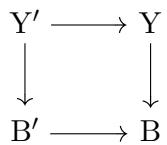
\includegraphics[keepaspectratio]{images/part001_f35053b2.jpg}}

is Cartesian.

Denote by \(q\) and \(q'\) the maps from X to Y and from \(X'\) to \(Y'\), respectively, induced by the maps \(p\) and \(p'\).

\[
\begin{array}{c} \mathrm {X^ {\prime}} \xrightarrow {f ^ {\prime}} \mathrm{X} \\ \Big \downarrow q ^ {\prime} \\ \mathrm {Y^ {\prime}} \xrightarrow {g} \mathrm{Y} \end{array}
\]

Since \(f\) is surjective, \(f'\) is also surjective; by Proposition 9 b), \(p\) is strict.

COROLLARY 1. --- Suppose that the map f is universally strict and surjective and that the map p' is universally strict. Then the map p is universally strict.

Let

\[
\begin{array}{c} \mathrm{Y} \xrightarrow {g ^ {\prime}} \mathrm{X} \\ \Biggl \downarrow q \\ \mathrm{C} \xrightarrow {g} \mathrm{B} \end{array}
\]

a Cartesian square; the goal is to prove that the map q is strict. By Remark 3 of I, p. 16, the squares

\[
\begin{array}{c} \mathrm {X^ {\prime}} \times_ {\mathrm{X}} \mathrm{Y} \xrightarrow {\mathrm{pr} _ {1}} \mathrm {X^ {\prime}} \\ \Biggl \downarrow r \\ \mathrm {B^ {\prime}} \times_ {\mathrm{B}} \mathrm{C} \xrightarrow {\mathrm{pr} _ {1}} \mathrm {B^ {\prime}} \end{array}
\]

and

\[
\begin{array}{c} \mathrm {X^ {\prime} \times_ {X} Y\xrightarrow {pr_ {2}} Y} \\ \Big \downarrow r \\ \mathrm {B^ {\prime} \times_ {B} C\xrightarrow {pr_ {2}} C} \end{array}\tag{21}
\]

are Cartesian, where \(r \colon X' \times_{X} Y \to B' \times_{B} C\) denotes the map induced by \((p', q)\). As the map \(f\) is universally strict and surjective, the same holds for the map \(\mathrm{pr}_2 \colon B' \times_{B} C \to C\) (I, p. 20, def. 6 and I, p. 10, cor. of prop. 4). On the other hand, the map \(r\) is strict, since \(p'\) is assumed to be universally strict. By Proposition 11, c) applied to the Cartesian square (21), the map \(q\) is strict.

COROLLARY 2. --- Let B and X be topological spaces and let \(p\colon X \to B\) be a continuous map. Let \((A_i)_{i \in I}\) be a family of subsets of B that is an open cover of B, or else a locally finite closed cover of B. If for every \(i \in I\), the map \(p_{A_i}\colon \overline{p}^1(A_i) \to A_i\) is strict (resp. universally strict), the map p is strict (resp. universally strict).

For every \(i \in \mathrm{I}\), set \(\mathrm{Y}_i = \overline{p}^{1}(\mathrm{A}_i)\) and \(p_i = p_{\mathrm{A}_i}\). Let A be the sum space of the family \((\mathrm{A}_i)_{i \in \mathrm{I}}\) and Y the sum space of the family \((\mathrm{Y}_i)_{i \in \mathrm{I}}\); let us denote by \(f: \mathrm{A} \to \mathrm{B}\) (resp. \(g: \mathrm{Y} \to \mathrm{X}\), \(q: \mathrm{Y} \to \mathrm{A}\)) the map induced by the family of canonical injections \(A_i \rightarrow B\) (resp. of canonical injections \(Y_i \rightarrow X\) and of the maps \(p_i\)). The square

\[
\begin{array}{c} \mathrm{Y} \xrightarrow {g} \mathrm{X} \\ \Big \downarrow q \\ \mathrm{A} \xrightarrow {f} \mathrm{B} \end{array}
\]

is a Cartesian square (Examples, I, p. 10 and p. 14). By the corollary, I, p. 20, the map \(f\) is universally strict. By Proposition 11, it therefore suffices to prove that the map \(q\) is strict (resp. universally strict) if the maps \(p_i\), for \(i \in I\), are strict (resp. universally strict). We are thus reduced to proving the corollary when the sets \(A_i\), \(i \in I\), form a partition of the space B into open and closed parts, which we will henceforth assume.

Suppose that each of the maps \(p_i\), \(i \in I\), is strict. If U is an open subset of X and is saturated for the equivalence relation defined by p, the set \(p_i(\mathrm{X}_i \cap \mathrm{U})\) is open in \(\mathrm{A}_i\) and \(p(\mathrm{U}) = \bigcup_{i \in \mathrm{I}} p_i(\mathrm{X}_i \cap \mathrm{U})\) is open in B. The map p is therefore strict.

Suppose now that each of the maps \(p_{i}, i \in I\), is universally strict, and let us show that the map p is universally strict. Let C be a topological space and \(h: C \to B\) a continuous map. The goal is to show that the map \(pr_{1}: X \times_{B} C \to C\) is strict. The space C is identified with the sum space of the family \(C_{i} = h^{-1}(A_{i})\), and the space \(X \times_{B} C\) is identified with the direct sum space of the family \(X \times_{B} C_{i} = X_{i} \times_{A_{i}} C_{i}\). Since \(p_{i}\) is universally strict, the map \(pr_{1}: X_{i} \times_{A_{i}} C_{i} \to C_{i}\) is strict. By the preceding, the map \(pr_{1}: X \times_{B} C \to C\) is strict. This proves that the map p is universally strict.

\section{ÉTALE MAPS}

\subsection{Separated maps}

PROPOSITION 1. --- Let X and Y be topological spaces, and let \(f\colon X \to Y\) be a continuous map. The following properties are equivalent:

\begin{enumerate}
\def\labelenumi{(\roman{enumi})}
\item
  The diagonal \(\Delta_{X}\) of the fibered product X \(\times_{Y}\) X is a closed subspace;
\item
  For every topological space W and every pair of continuous maps \((g_{1}, g_{2})\) from W into X such that \(f \circ g_{1} = f \circ g_{2}\) , the set of points \(w \in W\) such that \(g_{1}(w) = g_{2}(w)\) is closed in W;
\item
  For every pair \((x_{1}, x_{2})\) of points of X such that \(x_{1} \neq x_{2}\) and \(f(x_{1}) = f(x_{2})\) , there exists a neighborhood \(V_{1}\) of \(x_{1}\) in X and a neighborhood \(V_{2}\) of \(x_{2}\) in X such that \(V_{1} \cap V_{2} = \varnothing\) .
\end{enumerate}

(i)⇒(ii): Let \(g_{1}\) and \(g_{2}\) be continuous maps from W into X such that \(f \circ g_{1} = f \circ g_{2}\), and let \(g: W \to X \times_{Y} X\) be the map induced by \(g_{1}\) and \(g_{2}\). The set of points \(w \in W\) such that \(g_{1}(w) = g_{2}(w)\) is \(g^{-1}(\Delta_{X})\). Since g is continuous, it is therefore closed if the diagonal \(\Delta_{X}\) is closed.

(ii)⇒(i): The diagonal \(\Delta_{X}\) is the set of points \(z \in X \times_{Y} X\) such that \(\mathrm{pr}_{1}(z) = \mathrm{pr}_{2}(z)\). It follows from (ii), applied to \(W = X \times_{Y} X\) and to the pair of maps \((\mathrm{pr}_{1}, \mathrm{pr}_{2})\), that the diagonal \(\Delta_{X}\) is closed in \(X \times_{Y} X\).

(i)⇔(iii): Let \((x_{1}, x_{2})\) be a point of \(X \times_{Y} X\) and let \(V_{1}\) and \(V_{2}\) be neighborhoods of \(x_{1}\) and \(x_{2}\), respectively. The condition \(V_{1} \cap V_{2} = \varnothing\) is equivalent to the condition \((\mathrm{V}_{1} \times \mathrm{V}_{2}) \cap \Delta_{\mathrm{X}} = \varnothing\), that is, to \((\mathrm{V}_{1} \times \mathrm{V}_{2}) \cap (\mathrm{X} \times_{\mathrm{Y}} \mathrm{X}) \cap \Delta_{\mathrm{X}} = \varnothing\). Since the sets \((\mathrm{V}_{1} \times \mathrm{V}_{2}) \cap (\mathrm{X} \times_{\mathrm{Y}} \mathrm{X})\) form a base of neighborhoods of \((x_{1}, x_{2})\) in \(X \times_{Y} X\), this proves the equivalence of (i) and (iii).

DEFINITION 1. --- Let X and Y be topological spaces. A continuous map \(f: X \to Y\) is separated if it satisfies the equivalent conditions of Proposition 1.

PROPOSITION 2. --- Let X, Y, Z be topological spaces and let \(f\colon X \to Y\) and \(g\colon Y \to Z\) be continuous maps.

\begin{enumerate}
\def\labelenumi{\alph{enumi})}
\item
  If f and g are separated, then \(g \circ f\) is separated.
\item
If g \(\circ\) f is separated, then f is separated.
\item
  Suppose further that the map f is proper and surjective. Then, if g ∘ f is separated, g is separated.
\end{enumerate}

Consider, in X×X, the subspaces \(\Delta_{X}\) (diagonal), \(X \times_Y X\) and \(X \times_Z X\). These are respectively the sets of points u of X×X such that \(\mathrm{pr}_{1}(u)=\mathrm{pr}_{2}(u)\), \(f\circ\mathrm{pr}_{1}(u)=f\circ\mathrm{pr}_{2}(u)\), \(g\circ f\circ\mathrm{pr}_{1}(u)=g\circ f\circ\mathrm{pr}_{2}(u)\). If \(g\circ f\) is separated, \(\Delta_{X}\) is closed in \(X \times_Z X\), hence also in \(X \times_Y X\), whence b).

By Proposition 1, (ii), applied to W = X ×\_Z X, \(g_1 = f \circ \text{pr}_1\) and \(g_2 = f \circ \text{pr}_2\), X ×\_Y X is closed in X ×\_Z X if \(g\) is separated. If moreover \(f\) is separated, \(\Delta_X\) is closed in X ×\_Y X (Proposition 1, (i)), hence in X ×\_Z X, whence \(a\).

Finally, let us prove \(c\). The map \((f, f) \colon X \times X \to Y \times Y\) is proper (TG, I, p. 73, prop. 4). The subspace \(X \times_Z X\) is the inverse image of \(Y \times_Z Y\) under \((f, f)\); by TG, I, p. 72, prop. 3, the map \(u \colon X \times_Z X \to Y \times_Z Y\) induced by \((f, f)\) is proper. Since \(g \circ f\) is separated, the diagonal \(\Delta_X\) is closed in \(X \times_Z X\). Consequently, \(u(\Delta_X)\) is closed in \(Y \times_Z Y\). Since \(f\) is surjective, \(u(\Delta_X)\) is the diagonal of \(Y \times_Z Y\). This shows that \(g\) is separated.

Remarks. --- 1) An injective continuous map is separated.

\begin{enumerate}
\def\labelenumi{\arabic{enumi})}
\setcounter{enumi}{1}
\tightlist
\item
  For a topological space X to be Hausdorff (TG, I, p. 52, def. 1), it is necessary and sufficient that the map from X into a space reduced to a single point be separated. In this case, every continuous map from X into a topological space is separated (Proposition 1, (iii)).
\end{enumerate}

Let \(f\colon X \to Y\) be a continuous and separated map. For every point \(y\) of \(Y\), the fiber \(f^{-1}(y)\) is a separated topological space (loc. cit.). There nevertheless exist continuous maps which are not separated but all of whose fibers are separated topological spaces (I, p. 140, exerc. 1).

\begin{enumerate}
\def\labelenumi{\arabic{enumi})}
\setcounter{enumi}{2}
\item
  Let \(f \colon X \to Y\) be a continuous and separated map. If the space Y is separated, then the space X is separated. This follows from Remark 2 and Proposition 2 applied with a space Z reduced to a point.
\item
  Let \(f \colon X \to Y\) be a continuous and separated map, let \(y\) be a point of \(Y\), and let \(A\) be a finite subset of \(f^{-1}(y)\). Let us prove that there exists a family \((V_a)_{a \in A}\) of pairwise disjoint sets such that, for each \(a \in A\), the set \(V_a\) is a neighborhood of \(a\) in X. To do this, for each subset \(\{a,b\}\) of \(A\) with two elements, choose a neighborhood \(V_{(a,b)}\) of \(a\) and a neighborhood \(\mathrm{V}_{(b,a)}\) of \(b\) in X such that \(\mathrm{V}_{(a,b)} \cap \mathrm{V}_{(b,a)} = \varnothing\) (Proposition 1, (iii)). Let \(\mathrm{V}_a\) denote the intersection of the family formed by X and the sets \(\mathrm{V}_{(a,b)}\) for \(b \in \mathrm{A}\), \(b \neq a\). The set \(\mathrm{V}_a\) is a neighborhood of \(a\) in X, and if \(a\), \(b\) are two distinct elements of A, the set \(\mathrm{V}_a \cap \mathrm{V}_b\) is contained in \(\mathrm{V}_{(a,b)} \cap \mathrm{V}_{(b,a)}\), hence is empty.
\item
  Let \(Y\) be a topological space. Let \((\mathrm{A}_{i})_{i\in\mathrm{I}}\) be a family of subsets of Y and let X be the sum space of the family \((\mathrm{A}_{i})_{i\in\mathrm{I}}\). The canonical map from X to Y is separated.
\end{enumerate}

PROPOSITION 3. --- Let \(f\colon X \to Y\) be a continuous and separated map. Every continuous section of \(f\) induces a homeomorphism of \(Y\) onto a closed subset of \(X\).

Let \(s\colon Y \to X\) be a continuous section of \(f\). The map \(s\) induces a homeomorphism of \(Y\) onto the subspace \(s(Y)\) of \(X\) (TG, I, p. 22, prop. 9). The identity map of \(X\) and the map \(s \circ f\) are continuous and one has \(f \circ \mathrm {Id}_{X} = f \circ (s \circ f)\). Since the map \(f\) is separated, the set \(s(Y)\), which is the set of points \(x\) of \(X\) such that \(x = (s \circ f)(x)\), is closed in \(X\) (Proposition 1, (ii)).

PROPOSITION 4. --- Let

\pandocbounded{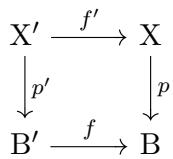
\includegraphics[keepaspectratio]{images/part001_94ec13ba.jpg}}

a Cartesian square. If the map p is separated, then so is p'. Conversely, if p' is separated and if f is universally strict and surjective, then p is separated.

Consider the square

\[
\begin{array}{c} \mathrm {X^ {\prime} \times_ {B^ {\prime}} X^ {\prime}} \xrightarrow {\varphi} \mathrm {X \times_ {B} X} \\ \Biggl \downarrow_ {q ^ {\prime}} \\ \mathrm {B^ {\prime} \xrightarrow {f} B} \end{array}
\]

where the map \(\varphi\) is induced by the map \(f' \times f': X' \times X' \to X \times X\) . Recall (I, p. 13, example 1) that this square is Cartesian and that one has \(\overline{\varphi}^1(\Delta_X) = \Delta_{X'}\) .

If the map p is separated, the set \(\Delta_{\mathrm{X}}\) is closed in \(\mathrm{X} \times_{\mathrm{B}} \mathrm{X}\); therefore, \(\Delta_{\mathrm{X}'}\) is a closed subset of \(\mathrm{X}' \times_{\mathrm{B}'} \mathrm{X}'\), which proves that the map \(p'\) is separated.

If the map f is surjective, the map \(\varphi\) is surjective (I, p. 10, cor.); if f is universally strict, \(\varphi\) is strict (I, p. 20, def. 6). Suppose the map \(p'\) is separated. Then \(\Delta_{\mathrm{X}'}\) is closed in \(\mathrm{X}' \times_{\mathrm{B}'} \mathrm{X}'\). Since \(\Delta_{\mathrm{X}'} = \overline{\varphi}^{1}(\Delta_{\mathrm{X}})\) and since \(\varphi\) is surjective and strict, \(\Delta_{\mathrm{X}}\) is closed in \(\mathrm{X} \times_{\mathrm{B}} \mathrm{X}\), which proves that the map \(p\) is separated.

PROPOSITION 5. --- Let \(f: X \to Y\) and \(g: Y \to Z\) be continuous maps. Suppose the map \(g\) is separated and the map \(g \circ f\) is proper. The map \(f\) is then proper.

Consider the following Cartesian square:

\[
\begin{array}{c} \mathrm{X} \times_ {\mathrm{Z}} \mathrm{Y} \xrightarrow {\operatorname{pr} _ {2}} \mathrm{Y} \\ \Biggl \downarrow \operatorname{pr} _ {1} \\ \mathrm{X} \xrightarrow {g \circ f} \mathrm{Z}. \end{array}
\]

Let \(s \colon X \to X \times_{Z} Y\) be the map \(x \mapsto (x, f(x))\). This is a continuous section of \(\mathrm{pr}_1 \colon X \times_{Z} Y \to X\). By Proposition 4, the map \(\mathrm{pr}_1\) is separated; it follows that the map \(s\) is proper (I, p. 27, prop. 3 and TG, I, p. 72, prop. 2). On the other hand, the map \(\mathrm{pr}_2\) is proper (I, p. 17, prop. 8). Therefore the map \(f\), which is equal to \(\mathrm{pr}_2 \circ s\), is proper (TG, I, p. 73, prop. 5).

\subsection{Étale maps}

DEFINITION 2. --- Let E and B be topological spaces, let \(p\colon\mathrm{E}\to\mathrm{B}\) be a map and let \(x\) be a point of E. One says that the map \(p\) is topologically étale at \(x\) if there exists a neighborhood U of \(x\) in E and a neighborhood V of \(p(x)\) in B such that \(p\) induces a homeomorphism from U onto V.

One says that the map p is topologically étale if it is topologically étale at every point x of E.

When there is no possible confusion (cf. Example 3 below), one says étale instead of topologically étale. Instead of saying that \(p\colon \mathrm{E}\to \mathrm{B}\) is an étale map, one also says that the B-space \((\mathrm{E},p)\) is an étale B-space, or simply that E is an étale space over B, when no doubt is possible as to the map \(p\).

Remarks. --- 1) The set of points of E at which a map \(p \colon \mathrm{E} \to \mathrm{B}\) is étale is an open subset U of E and the restriction of p to U is an étale map from U to B.

\begin{enumerate}
\def\labelenumi{\arabic{enumi})}
\setcounter{enumi}{1}
\tightlist
\item
  An étale map is continuous and open (TG, I, p. 33, prop. 5); in particular, the image of an étale map is open. Conversely, if \(p \colon \mathrm{E} \to \mathrm{B}\) is a continuous and open mapping, and if every point x of E has a neighborhood V such that the map \(p \mid \mathrm{V}\) is injective, the map p is étale. The fibers of an étale map are discrete.
\end{enumerate}

Examples. --- 1) Let B be a topological space and \((\mathrm{U}_{i})_{i\in\mathrm{I}}\) a family of subsets of B. Let E denote the sum space of the family \((\mathrm{U}_{i})_{i\in\mathrm{I}}\) and \(p: E \to B\) the map induced by the canonical injections of the \(U_{i}\) in B. For the map p to be étale, it is necessary and sufficient that the \(U_{i}\), \(i \in I\), all be open.

\begin{enumerate}
\def\labelenumi{\arabic{enumi})}
\setcounter{enumi}{1}
\item
For a holomorphic function \(f\colon U \to \mathbf{C}\) to be an étale map, it is necessary and sufficient that its derivative does not vanish.
\item
  An étale morphism of varieties (VAR, R, 5.7.8) is a topologically étale map, but there exist morphisms of real varieties that are topologically étale and are not étale morphisms. This is the case, for example, of the map \(x \mapsto x^3\) from \(\mathbf{R}\) into \(\mathbf{R}\). However, a morphism of complex analytic varieties that is topologically étale is an étale morphism (I, p. 141, exerc. 6).
\end{enumerate}

PROPOSITION 6. — Let X, Y, Z be topological spaces and let \(f\colon X\to Y\) , \(g\colon Y\to Z\) be maps.

\begin{enumerate}
\def\labelenumi{\alph{enumi})}
\item
  Suppose that f and g are étale; then \(g \circ f\) is étale.
\item
  Suppose that \(g\) is étale, \(f\) is continuous and \(g \circ f\) is open. Then \(f\) is open.
\item
  Suppose that \(g \circ f\) and \(g\) are étale and that \(f\) is continuous. The map \(f\) is then étale.
\item
  Suppose that \(g \circ f\) is étale and that the map \(f\) is continuous and open; then, \(f\) is étale and \(g\) is étale at every point of \(f(\mathrm{X})\) .
\end{enumerate}

Let us prove (a). Suppose that \(f\) and \(g\) are étale. They are then continuous and open, so the map \(g \circ f\) is continuous and open. Let \(x\) be a point of X. There exists a neighborhood W of \(f(x)\) in Y such that \(g \mid \mathrm{W}\) is injective, and a neighborhood V of \(x\) in X, contained in \(f(\mathrm{W})\), such that \(f \mid \mathrm{V}\) is injective; the map \((g \circ f) \mid \mathrm{V}\) is then injective. This proves that the map \(g \circ f\) is étale (Remark 2).

Let us prove b). Let x be a point of X and W an open neighborhood of \(f(x)\) such that g induces a homeomorphism from W onto the open set \(g(\mathrm{W})\). Let V be a neighborhood of x such that \(f(\mathrm{V})\) is contained in W; then, \(g \circ f(\mathrm{V})\) is a neighborhood of \(g \circ f(x)\), therefore \(f(\mathrm{V})\) is a neighborhood of \(f(x)\) in the open set W, and also in Y. This proves that the map f is open (TG, I, p. 33, prop. 5).

Let us prove c). By b), f is open. Let x be a point of X. Since \(g \circ f\) is étale, there exists a neighborhood V of x in X such that \(g \circ f \mid V\) is injective. Thus, \(f \mid V\) is injective and f is étale (I, p. 29, remark 2).

Let us prove d). Let \(x\) be a point of \(X\) and set \(y = f(x)\). There exists an open neighborhood \(V\) of \(x\) such that \(g \circ f\) induces a homeomorphism from \(V\) onto the open set \(g \circ f(V)\). As the map \(f\) is open, \(f(V)\) is an open neighborhood of \(y\). The map \(f|_V\colon V \to f(V)\) induced by \(f\) by passing to subspaces is continuous, open, and bijective; it is therefore a homeomorphism, so that \(f\) is étale at \(x\). Moreover, the map \(g\) induces a homeomorphism of \(f(V)\) onto \(g \circ f(V)\), hence is étale at \(y\).

COROLLARY 1. — Let B be a topological space. A B-morphism from one étale B-space to another is étale.

This follows from assertion c) of Prop. 6.

COROLLARY 2. --- Let B be a topological space; a bijective B-morphism from one étale B-space to another is a B-isomorphism.

By corollary 1, such a morphism is étale; it is therefore open (I, p. 29, remark 2). If it is bijective, it is a B-isomorphism.

COROLLARY 3. --- Let p: E → B be an étale map. Every continuous section of p induces a homeomorphism of B onto an open subset of E.

Indeed, such a section is étale (corollary 1), hence open.

COROLLARY 4. --- Let p: E → B be an étale and separated map. Suppose that E is connected and that p admits a section. Then p is a homeomorphism.

Let \(s\) be a section of \(p\) ; since \(p\) is étale, the image of \(s\) is open in E (Corollary 3); it is also closed, since \(p\) is separated (I, p. 27, prop. 3). Since E is connected, we have \(s(\mathrm{B}) = \mathrm{E}\) and \(p\) is a homeomorphism.

PROPOSITION 7. --- Let \(p\colon E \to B\) be a continuous map. For the map \(p\) to be étale, it is necessary and sufficient that it be open and that the diagonal \(\Delta_{E}\) of \(E \times_{B} E\) be open in \(E \times_{B} E\).

Suppose first that the map p is étale. Then it is open and every point of E has a neighborhood V such that \(p|V\) is injective, which amounts to saying that one has \((\mathrm{V} \times \mathrm{V}) \cap (\mathrm{E} \times_{\mathrm{B}} \mathrm{E}) \subset \Delta_{\mathrm{E}}\) . Therefore, \(\Delta_{E}\) is an open subset of \(E \times_{B} E\) .

Conversely, suppose that p is an open mapping and that \(\Delta_{\mathrm{E}}\) is an open subset of \(\mathrm{E} \times_{\mathrm{B}} \mathrm{E}\) . Let x be a point of E. Let V be an open neighborhood of x in E such that \((\mathrm{V} \times \mathrm{V}) \cap (\mathrm{E} \times_{\mathrm{B}} \mathrm{E})\) is contained in \(\Delta_{\mathrm{E}}\) . Then, \(p \mid \mathrm{V}\) is injective. By Remark 2, I, p. 29, the map p is étale.

PROPOSITION 8. --- Let

\pandocbounded{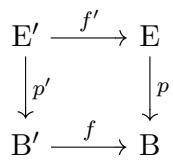
\includegraphics[keepaspectratio]{images/part001_e4ab0ebd.jpg}}

a Cartesian square. If the morphism p is étale, then the morphism p' is étale. Conversely, if the morphism p' is étale and the morphism f is universally strict and surjective, then the morphism p is étale.

Suppose that the map p is étale. In particular, it is open and \(p'\) is open (I, p. 17, prop. 8). Consider then the Cartesian square (I, p. 13, example 1)

\[
\begin{array}{c} \mathrm{E} ^ {\prime} \times_ {\mathrm{B} ^ {\prime}} \mathrm{E} ^ {\prime} \xrightarrow {\varphi} \mathrm{E} \times_ {\mathrm{B}} \mathrm{E} \\ \Biggl \downarrow q ^ {\prime} \qquad \qquad \qquad \qquad \Biggl \downarrow q \\ \mathrm{B} ^ {\prime} \xrightarrow {f} \mathrm{B}. \end{array}
\]

We have \(\Delta_{\mathrm{E}^{\prime}} = \overline{\varphi}^{1}(\Delta_{\mathrm{E}})\) (loc. cit.). Moreover, the diagonal \(\Delta_{\mathrm{E}}\) is open in \(\mathrm{E} \times_{\mathrm{B}} \mathrm{E}\) (prop. 7), hence the diagonal \(\Delta_{\mathrm{E}^{\prime}}\) is open in \(\mathrm{E}^{\prime} \times_{\mathrm{B}^{\prime}} \mathrm{E}^{\prime}\). This proves that the map \(p^{\prime}\) is étale (loc. cit.).

Suppose now that the map \(f\) is surjective and universally strict, and let the map \(p'\) be étale. Then, \(p'\) is open, therefore \(p\) is open (I, p. 21, prop. 11, \(a\)). On the other hand \(\Delta_{\mathrm{E}'}\) is an open subset of \(\mathrm{E}' \times_{\mathrm{B}'} \mathrm{E}'\). Since \(\Delta_{\mathrm{E}'} = \overline{\varphi}^{1}(\Delta_{\mathrm{E}})\) and the map \(\varphi\) is surjective and strict (I, p. 20, def. 6), \(\Delta_{\mathrm{E}}\) is open in \(\mathrm{E} \times_{\mathrm{B}} \mathrm{E}\). By prop. 7, the map p is étale.

COROLLARY. --- Let B be a topological space. The fiber product of two étale B-spaces is an étale B-space.

Let \((\mathrm{E}, p)\) and \((\mathrm{E}^{\prime}, p^{\prime})\) be étale B-spaces. The map \(pr_{1}: E \times_{B} E^{\prime} \to E\) is étale (prop. 8), hence the map \(p \circ pr_{1}: E \times_{B} E^{\prime} \to B\) is étale (prop. 6, a)).

Remark 3. --- Let

\pandocbounded{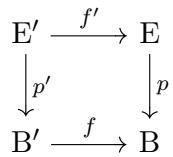
\includegraphics[keepaspectratio]{images/part001_b818a80c.jpg}}

a Cartesian square. If the map p is étale and the map f is strict, then the map \(f'\) is strict. Indeed, under these hypotheses, every point of E has an open neighborhood U such that p induces a homeomorphism from U onto the open set \(p(\mathrm{U})\) . The map \(p'\) induces then a homeomorphism of \((f')^{-1}(\mathrm{U})\) onto \(f^{-1}(p(\mathrm{U}))\). The map f induces a strict map from \(f^{-1}(p(\mathrm{U}))\) onto \(p(\mathrm{U})\) (I, p. 20) and the map \(f'\) therefore induces a strict map from \((f')^{-1}(\mathrm{U})\) into U. It follows that the map \(f'\) is strict (I, p. 23, corollary 2).

\subsection{Local sections of étale maps}

Let E and B be sets, A a subset of B, and \(p: E \rightarrow B\) a map. A section of p over A (or on A) is a map \(s: A \rightarrow E\) such that \(p \circ s\) is the canonical injection of A into B. The data of a section s of p over A is equivalent to the data of a section of the map \(p_{\mathrm{A}} \colon \overline{p}^{1}(\mathrm{A}) \to \mathrm{A}\) induced by p. If s is a section of p over A and if \(A'\) is a subset of A, the restriction \(s'\) of s to \(A'\) is a section of p over \(A'\). We then say that s is an extension of \(s'\) to A.

When E and B are topological spaces and \(p \colon \mathrm{E} \to \mathrm{B}\) is a continuous map, the set \(\mathcal{C}_{\mathrm{B}}(\mathrm{A};\mathrm{E})\) (I, p. 2) of continuous sections of \(p\) over A is also denoted by \(\mathcal{S}(\mathrm{A};p)\) or \(\mathcal{S}(\mathrm{A};\mathrm{E})\). Let \(s\) be a continuous section of \(p\) over A. The map \(s\) induces a homeomorphism of A onto \(s(\mathrm{A})\), and \(p\) induces the inverse homeomorphism. By Definition 2, I, p. 28, we therefore have:

PROPOSITION 9. --- Let p: E → B be a continuous map. For p to be étale, it is necessary and sufficient that every point of E have an open neighborhood which is the image of a continuous section of p over an open subset of B.

Remarks. --- 1) Let \(p \colon \mathrm{E} \to \mathrm{B}\) be a continuous and open map. For an open set U of E to be the image of a continuous section of \(p\) over an open set of B, it is necessary and sufficient that the restriction of \(p\) to U be injective.

\begin{enumerate}
\def\labelenumi{\arabic{enumi})}
\setcounter{enumi}{1}
\tightlist
\item
  Let \(p \colon \mathrm{E} \to \mathrm{B}\) a continuous map. Suppose that every point of B has an open neighborhood V such that there exists a continuous section of \(p\) over V. Such a map \(p\) is not necessarily étale, nor even open. It is nevertheless surjective and universally strict (I, p. 20, corollary).
\end{enumerate}

\subsection{Continuous liftings of étale maps}

Let \(p \colon \mathrm{E} \to \mathrm{B}\) and \(f \colon \mathrm{Z} \to \mathrm{B}\) be continuous maps. A continuous lifting of \(f\) to \(\mathrm{E}\) is called a continuous map \(g \colon \mathrm{Z} \to \mathrm{E}\) such that \(p \circ g = f\). The set of continuous liftings of \(f\) to \(\mathrm{E}\) is none other than \(\mathcal{C}_{\mathrm{B}}(\mathrm{Z};\mathrm{E})\). It is also identified with the set \(\mathcal{S}(\mathrm{Z};\mathrm{Z} \times_{\mathrm{B}}\mathrm{E})\) of continuous sections of the projection of the Z-space \((\mathrm{Z} \times_{\mathrm{B}}\mathrm{E},\mathrm{pr}_{1})\).

If T is a subset of Z, a continuous lifting of f to E defined on T is called a continuous lifting of f \textbar{} T to E:

\pandocbounded{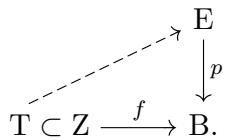
\includegraphics[keepaspectratio]{images/part001_46887bc2.jpg}}

PROPOSITION 10. --- Let E, B and Z be topological spaces, \(p\colon E \to B\) an étale map and \(f\colon Z \to B\) a continuous map.

Let \(z \in \mathbf{Z}\) and \(x \in \mathrm{E}\) be points such that \(f(z) = p(x)\). There exists a neighborhood \(\mathrm{W}\) of \(z\) on \(\mathbf{Z}\) and a continuous lifting \(g\) of \(f\) to \(\mathrm{E}\), defined on \(\mathrm{W}\), such that \(g(z) = x\).

There exists an open neighborhood V of \(p(x)\) in B and a continuous section s of p over V such that \(s(p(x)) = x\) (Proposition 9). The set \(W = f^{-1}(V)\) is an open neighborhood of z and the map \(g = s \circ (f|W)\) is a continuous lifting of f to E, defined on W and such that \(g(z) = x\).

PROPOSITION 11. --- Let E, B, and Z be topological spaces, let \(p\colon E \to B\) and \(f\colon Z \to B\) be continuous maps. Let \(g\) and \(g'\) be continuous liftings of \(f\) to E. Let W be the set of points of Z where \(g\) and \(g'\) coincide.

\begin{enumerate}
\def\labelenumi{\alph{enumi})}
\item
  If the map p is separated, W is closed.
\item
  If the map p is étale, W is open.
\end{enumerate}

Denote by \(h\) the continuous map \((g, g')\colon Z \to E \times E\). The image of \(h\) is contained in \(E \times_{B} E\) since \(p \circ g = f = p \circ g'\), and the set W of points of Z where g and g' coincide is the inverse image under \(h\) of the diagonal \(\Delta_{E}\).

If the map p is étale, the diagonal \(\Delta_{E}\) is open in \(E \times_{B} E\) (I, p. 31, prop. 7), hence the set W is open in Z.

If the map p is separated, the diagonal \(\Delta_{E}\) is closed in \(E \times_{B} E\) (I, p. 25, def. 1) and the set W is closed in Z.

COROLLARY 1. --- If the space Z is connected and if the map p is étale and separated, then continuous liftings of f to E that coincide at one point are equal.

COROLLARY 2. --- Let \(p\colon E \to B\) be a separated étale map. If the space E is connected, the group \(\mathrm{Aut}_{\mathrm{B}}(\mathrm{E})\) acts freely on E.

Indeed, if \(f: \mathrm{E} \to \mathrm{E}\) is a B-morphism, the set of points where f and \(\mathrm{Id}_{\mathrm{E}}\) coincide is E or the empty set by Cor. 1.

COROLLARY 3. --- Let E, B, and Z be topological spaces, let \(p\colon E \to B\) be a separated étale morphism, and let \(f\colon Z \to B\) be a continuous map. For \(i = 1,2\), let \(U_i\) be an open (resp. closed) subset of Z and \(g_i\colon U_i \to E\) be a continuous lifting of f defined on \(U_i\). Assume that the intersection \(U_1 \cap U_2\) is connected and that there exists a point z of \(U_1 \cap U_2\) such that \(g_1(z) = g_2(z)\). Then there exists a continuous lifting of f defined on \(U_1 \cup U_2\) which extends \(g_1\) and \(g_2\).

By corollary 1, the restrictions to \(U_{1} \cap U_{2}\) of \(g_{1}\) and \(g_{2}\) are equal. The map \(g: U_{1} \cup U_{2} \to E\) defined by \(g(z) = g_{i}(z)\) for \(z \in U_{i}\) (i = 1, 2) is a continuous lifting of f defined on \(U_{1} \cup U_{2}\) (TG, I, p. 19, prop. 4).

In the preceding results, the special case where Z = B and \(f = Id_{B}\) is important: the continuous liftings of f are then the continuous sections of p.

PROPOSITION 12. --- Let \(p \colon E \to B\) be an étale map. For the map \(p\) to be separated, it is necessary and sufficient that for every open subset \(V\) of \(B\) and every pair \((s, s')\) of continuous sections of \(p\) over \(V\), the set of points where \(s\) and \(s'\) coincide be closed in \(V\).

The condition is necessary (Proposition 11, I, p. 34). Let us prove that it is sufficient. Let \(b\) be a point of B, and let \(x\) and \(x'\) be two distinct points of E such that \(p(x) = p(x') = b\). Let V be an open neighborhood of b and s, s' continuous sections of p over V such that \(s(\mathrm{V})\) and \(s'(\mathrm{V})\) are open neighborhoods of x and x', respectively (Proposition 9). By hypothesis, the set W of points \(x \in \mathrm{V}\) such that \(s(x) \ne s'(x)\) is open in V, hence in B. The sets \(s(\mathrm{W})\) and \(s'(\mathrm{W})\) are open neighborhoods of x and x', respectively; they are disjoint by construction. This proves that the map p is separated (I, p. 25, Definition 1).
% semantic-fragments: legacy-input-seam
\relax{}
\subsection{Construction of continuous sections of étale maps}

THEOREM 1. --- Let X, Y, Z be topological spaces, let \(f: \mathrm{Z} \to \mathrm{X} \times \mathrm{Y}\) be a separated étale morphism, and let \(y_0\) be a point of Y. Let \(s: X \times Y \to Z\) be a section of \(f\) . Assume that the restriction of \(s\) to \(X \times \{y_0\}\) is continuous, as are the restrictions of \(s\) to \(\{x\} \times Y\) for all \(x \in X\). If the space \(Y\) is connected and locally connected (TG, I, p.~84, def. 4), the map \(s\) is continuous.

Lemma. --- Let U be an open subset of X, let V be a connected open subset of Y, and let \((x_{1},y_{1})\in\mathrm{U}\times\mathrm{V}\). Assume that the restriction of s to \(U\times\{y_{1}\}\) is continuous. Let \(\sigma\) be a continuous section of f over \(U\times V\) such that \(\sigma(x_{1},y_{1})=s(x_{1},y_{1})\) . There exists a neighborhood \(U'\) of \(x_{1}\) such that \(s=\sigma\) on \(U'\times V\). In particular, the map s is continuous in a neighborhood of \((x_{1},y_{1})\) .

Since the restriction of \(s\) to \(\mathrm{U} \times \{y_1\}\) is continuous and the map \(f\) is étale, there exists a neighborhood \(\mathrm{U}'\) of \(x_1\) such that \(s(x, y_1) = \sigma(x, y_1)\) for all \(x \in \mathrm{U}'\) (I, p.~34, prop. 11, b)). Let \(x \in \mathrm{U}'\) ; since the restriction of \(s\) to \(\{x\} \times \mathrm{V}\) is continuous and the map \(f\) is étale and separated, it follows from cor. 1, I, p.~34 that \(\sigma(x, y) = s(x, y)\) for all \(y \in \mathrm{V}\) . Thus, \(s\) and \(\sigma\) coincide on \(\mathrm{U}' \times \mathrm{V}\) .

Let us now prove the theorem. Let us first prove that the map s is continuous in a neighborhood of every point of \(X \times \{y_{0}\}\) . Let \(x_{0} \in X\) ; one can choose an open neighborhood U of \(x_{0}\) in X, a connected open neighborhood V of \(y_{0}\) in Y and a continuous section \(\sigma: U \times V \to Z\) of f such that \(\sigma(x_{0}, y_{0}) = s(x_{0}, y_{0})\) . By the lemma above, s is continuous in a neighborhood of \((x_{0}, y_{0})\) .

We now prove that the map \(s\) is continuous at every point of \(\mathrm{X} \times \mathrm{Y}\) . For \(x_0 \in \mathrm{X}\) , denote by \(\mathrm{C}(x_0)\) the set of points \(y \in \mathrm{Y}\) such that \(s\) is continuous in a neighborhood of \((x_0, y)\) . The set \(\mathrm{C}(x_0)\) is open in Y by definition, and contains \(y_0\) by the preceding.

Let us prove that it is closed in Y. Consider a point \(y_{1}\) of Y adherent to \(\mathrm{C}(x_{0})\) , an open neighborhood U of \(x_{0}\) in X, an open neighborhood V of \(y_{1}\) in Y, and a continuous section \(\sigma\colon U\times V\to Z\) of f such that \(\sigma(x_{0},y_{1})=s(x_{0},y_{1})\) . Since the restriction of s to \(\{x_{0}\}\times V\) is continuous and f is étale, there exists an open neighborhood \(V^{\prime}\) of \(y_{1}\) in Y such that \(\sigma(x_{0},y)=s(x_{0},y)\) for all \(y\in V^{\prime}\) (prop. 11 of I, p.~34). Since Y is locally connected, we may assume that \(V^{\prime}\) is connected. Since \(y_{1}\) is adherent to \(\mathrm{C}(x_{0})\), the set \(\mathrm{C}(x_{0})\cap\mathrm{V}^{\prime}\) is nonempty; let \(y_{2}\) be a point of \(\mathrm{C}(x_{0})\cap\mathrm{V}^{\prime}\) . By the lemma applied to \((x_{0},y_{2})\) , there exists a neighborhood \(U^{\prime}\) of \(x_{0}\) contained in U such that \(s=\sigma\) over \(U^{\prime} \times V^{\prime}\) . This proves that \(\mathrm{C}(x_{0})\) is closed, because \(U^{\prime} \times V^{\prime}\) is a neighbourhood of \((x_{0}, y_{1})\) . Since Y is connected, we have \(\mathrm{C}(x_{0}) = \mathrm{Y}\) , and this for every \(x_{0} \in X\) , whence the theorem.

COROLLARY 1. --- Let X, Y, E, B be topological spaces. Let \(p\colon E \to B\) be an étale and separated map, and let \(h\colon X \times Y \to B\) be a continuous map and let \(y_0\) be a point of Y. Let \(g\colon X \times Y \to E\) be a map such that \(p \circ g = h\) . Suppose that the restrictions of \(g\) to \(X \times \{y_0\}\) on the one hand and, for every \(x \in X\) , to \(\{x\} \times Y\) on the other hand, are continuous. If the space Y is connected and locally connected, the map \(g\) is continuous.

Let Z be the fibered product \((\mathrm{X} \times \mathrm{Y}) \times_{\mathrm{B}} \mathrm{E}\) and \(f: Z \to X \times Y\) and \(h': Z \to E\) be the canonical projections. The map f is étale (I, p.~31, prop. 8) and separated (I, p.~27, prop. 4). The map \(s: X \times Y \to Z\) defined by \(s(x, y) = ((x, y), g(x, y))\) is a section of f which satisfies the hypotheses of Theorem 1. It is therefore continuous, as is \(g = h' \circ s\) .

Remark. --- If, in Theorem 1, one does not assume that the space Y is locally connected, the conclusion of the theorem is no longer necessarily valid (I, p.~141, exerc. 7).

THEOREM 2. --- Let B be a topological space and A a subspace of B. Assume one of the following hypotheses:

\begin{enumerate}
\def\labelenumi{(\roman{enumi})}
\item
  A has a fundamental system of paracompact neighborhoods;
\item
  B is paracompact and A is closed;
\item
  B is metrizable;
\item
  A is compact and any two distinct points of A have disjoint neighborhoods in B.
\end{enumerate}

Then, every continuous section over A of an étale map \(p\colon E \to B\) extends to a continuous section of \(p\) over a neighborhood of A.

Consider the following property (PCV) of the pair (B, A):

(PCV) For every covering \((\mathrm{U}_{i})_{i\in\mathrm{I}}\) of A by open subsets of B, there exists a neighborhood V of A and a locally finite family \((\mathrm{F}_{j})_{j\in\mathrm{J}}\) of closed subsets of V covering V, such that each of the \(F_{j}\) is contained in one of the \(U_{i}\) .

Theorem 2 follows from Lemmas 1 and 3 below.

Lemma 1. --- Each of the properties (i) to (iv) of Theorem 2 implies property (PCV).

Let \((\mathrm{U}_{i})_{i\in\mathrm{I}}\) be a covering of A by open subsets of B. Under hypothesis (i), there exists a paracompact neighborhood V of A contained in the union of the \(U_{i}\) , an open covering \((\mathrm{U}_{j}^{\prime})_{j\in\mathrm{J}}\) of the space V, locally finite and finer than the covering \((\mathrm{V}\cap\mathrm{U}_{i})_{i\in\mathrm{I}}\) , and an open covering \((\mathrm{U}_{j}^{\prime\prime})_{j\in\mathrm{J}}\) of the space V such that for every \(j\in J\) , the closure \(F_{j}\) of \(U_{j}^{\prime\prime}\) in V is contained in \(U_{j}^{\prime}\) (TG, IX, p.~49, prop. 4 and p.~48, cor. 1 to th. 3). Hence (PCV) in this case.

Condition (ii) implies condition (i) by Corollary 2 of TG, IX, p.~50. Likewise, condition (iii) implies condition (i): indeed, if B is metrizable, every neighborhood of A is metrizable, hence paracompact (TG, IX, p.~51, th. 4).

Finally suppose condition (iv) is satisfied and let us show that property (PCV) holds. Since A is compact, it suffices to consider the case of a finite covering \((\mathrm{U}_{i})_{0\leqslant i\leqslant n}\) . Let us then construct by induction open sets \(V_{0},\ldots,V_{n}\) of B satisfying the following conditions for \(0\leqslant i\leqslant n\) :

\(\alpha)\mathrm{A}\subset \mathrm{V}_{0}\cup \dots \cup \mathrm{V}_{i}\cup \mathrm{U}_{i + 1}\cup \dots \cup \mathrm{U}_{n};\)

\(\beta)\overline{\mathrm{V}_{i}}\cap \mathrm{A}\subset \mathrm{U}_{i}.\)

Suppose \(V_{0},\ldots,V_{r-1}\) have been constructed satisfying the above conditions for \(0\leqslant i\leqslant r-1\) , and let us construct \(V_{r}\) . The sets \(K=A\cap C U_{r}\) and \(L=A\cap C(V_{0}\cup\cdots\cup V_{r-1}\cup U_{r+1}\cup\cdots\cup U_{n})\) are closed in A, hence compact. By virtue of \((\alpha)\) , they are disjoint. By hypothesis, for every point a of L and every point b of K, there exist disjoint neighborhoods of a and b in B. By Lemma 2 below, there exist open sets \(V_{r}\) and W in B, disjoint and such that \(L\subset V_{r}\) and \(K\subset W\) . From the inclusions \(L\subset V_{r}\) and \(A\subset V_{0}\cup\cdots\cup V_{r-1}\cup U_{r}\cup\cdots\cup U_{n}\) and the definition of L, one deduces \((\alpha)\) for i=r. On the other hand, one has \(\overline{V_{r}}\cap K=\varnothing\) , whence \(\overline{V_{r}}\cap A\subset U_{r}\) .

The set \(M = \bigcup_{0 \leqslant i \leqslant n} (\overline{\mathrm{V}_{i}} \cap \mathbb{C}\mathrm{U}_{i})\) is closed and does not meet A by ( \(\beta\) ). By ( \(\alpha\) ), the set \(V = (\bigcup_{0 \leqslant i \leqslant n} \overline{\mathrm{V}_{i}}) - M\) is a neighborhood of A in B. For \(i = 0, \ldots, n\) , set \(F_{i} = V \cap \overline{V_{i}}\); it is a closed subset of V, contained in \(U_{i}\) . The family \((F_{i})_{0 \leqslant i \leqslant n}\) is a covering of V, hence property (PCV) holds.

Lemma 2. --- Let B be a topological space, and let K and L be quasi-compact subsets of B. Suppose that for every point a of K and every point b of L, there exist disjoint neighborhoods of a and b in B. Then there exist two disjoint open sets U and V in B such that K ⊂ U and L ⊂ V.

Let \(a\) be a point of K. For every \(b \in L\) , let \(U_{a,b}\) and \(V_{a,b}\) be disjoint open neighborhoods of \(a\) and of \(b\) . For \(a\) fixed, the family \((V_{a,b})_{b \in L}\) is an open cover of L. Since L is quasi-compact, there exists a finite family \(T_a \subset L\) such that the union \(V_b\) of the \(V_{a,b}\) for \(b \in T_a\) contains L. The intersection \(U_a\) of the \(U_{a,b}\) for \(b \in T_a\) is an open neighborhood of \(a\) since \(T_a\) is finite; moreover, \(U_a\) and \(V_a\) are disjoint. The \((U_a)_{a \in A}\) form an open covering of K. Since K is quasi-compact, there exists a finite family \(S \subset K\) such that \(U = \bigcup_{a \in S} U_a\) contains K. Then, \(V = \bigcap_{a \in S} V_a\) is an open subset of B containing L. The lemma is proved.

Lemma 3. --- Let B be a topological space and A a subspace of B such that the pair (B,A) satisfies property (PCV) of I, p.~37. Then, every continuous section over A of an étale map \(p\colon E \to B\) extends to a continuous section of \(p\) over a neighborhood of A.

Let \(p \colon \mathrm{E} \to \mathrm{B}\) be an étale map and \(s \colon \mathrm{A} \to \mathrm{E}\) a continuous section of \(p\) over A. For every point \(a\) of A, there exists an open neighborhood \(\mathrm{U}_a\) of \(a\) and a continuous section \(s_a \colon \mathrm{U}_a \to \mathrm{E}\) which coincides with \(s\) on \(\mathrm{U}_a \cap \mathrm{A}\) (I, p.~34, prop. 10 and I, p.~34, prop. 11). The family \((\mathrm{U}_a)_{a \in \mathrm{A}}\) is a covering of A by open sets of B. Let V be a neighborhood of A in B, let \((\mathrm{F}_j)_{j \in \mathrm{J}}\) be a locally finite family of closed subsets of V covering V, and let \(a \colon \mathrm{J} \to \mathrm{A}\) be a map such that \(\mathrm{F}_j\) is contained in \(\mathrm{U}_{a(j)}\) for all \(j \in \mathrm{J}\) (property (PCV)). Let us denote by \(s_j\) the restriction of \(s_{a(j)}\) to \(\mathrm{F}_j\) . Let W be the set of points \(b \in \mathrm{V}\) satisfying \(s_j(b) = s_k(b)\) for every pair \((j, k) \in \mathrm{J} \times \mathrm{J}\) such that \(b \in \mathrm{F}_j \cap \mathrm{F}_k\). We define a section \(s' \colon \mathrm{W} \to \mathrm{E}\) by \(s'(b) = s_j(b)\) if \(b \in \mathrm{F}_j\) . We have \(\mathrm{A} \subset \mathrm{W}\) and \(s' | \mathrm{A} = s\). The section \(s'\) is continuous by prop. 4 of I, p.~19.

It remains to prove that W is a neighbourhood of A in B. For every pair \((j,k)\in\mathrm{J}\times\mathrm{J}\) , denote by \(T_{jk}\) the set of points \(b\in F_{j}\cap F_{k}\) such that \(s_{j}(b)\neq s_{k}(b)\) . The set \(T_{jk}\) is closed in \(F_{j}\cap F_{k}\) (prop. 11, b) of I, p.~34), hence in V, and the sets \(T_{jk}\) form a locally finite family of subsets of V. The union T of the family \((T_{jk})\) is therefore a closed set in V (TG, I, p.~6, prop. 4). Now W is, by definition, the complement of T in V. It is therefore a neighbourhood of A in V and consequently in B.

\subsection{Upper bound for the cardinality of the fibres of an étale and separated map}

THEOREM 3. --- Let E and B be topological spaces and p: E → B an étale and separated map. Suppose that E is connected and that B is locally connected. Let W be a base of the topology of B. Then, for every point a of B, one has Card(E \(_{a}\) ) ≤ sup(Card(W), Card(N)).

Since the space B is locally connected, its topology has a base \(\mathcal{W}'\) consisting of connected open sets, for example the connected components of the open sets of \(\mathcal{W}\) (TG, I, p.~85, prop. 11). By virtue of Lemma 4 below, there exists a base \(\mathcal{V}\) of the topology of B composed of connected open sets and such that \(\mathrm{Card}(\mathcal{V}) \leqslant \mathrm{Card}(\mathcal{W})^2\) .

Lemma 4. --- Let B be a topological space and let W and W' be bases of the topology of B. There exists a subset V of W' which is a base of the topology of B and such that \(\text{Card}(\mathcal{V}) \leqslant \text{Card}(\mathcal{W})^{2}\) .

Let \(\mathcal{A} \subset \mathcal{W} \times \mathcal{W}\) be the set of pairs \((\mathrm{W}_1, \mathrm{W}_2)\) for which there exists \(\mathrm{W}' \in \mathcal{W}'\) such that \(\mathrm{W}_1 \subset \mathrm{W}' \subset \mathrm{W}_2\) ; let \(\varphi: \mathcal{A} \to \mathcal{W}'\) be a map such that one has \(\mathrm{W}_1 \subset \varphi(\mathrm{W}_1, \mathrm{W}_2) \subset \mathrm{W}_2\) for every pair \((\mathrm{W}_1, \mathrm{W}_2) \in \mathcal{A}\) , and let \(\mathcal{V} \subset \mathcal{W}'\) be the image of \(\varphi\) . We have

\[
\operatorname{Card} (\mathcal {V}) \leqslant \operatorname{Card} (\mathcal {A}) \leqslant \operatorname{Card} (\mathcal {W} \times \mathcal {W})
\]

(E, III, p.~25, prop. 3). Let us prove that V is a base of the topology of B. Let x be a point of B and U a neighbourhood of x. By hypothesis, x admits a neighbourhood \(W_{2} \in W\) contained in U, a neighbourhood \(W' \in W'\) contained in \(W_{2}\) and a neighbourhood \(W_{1} \in W\) contained in \(W'\) . One thus has \(W_{1} \subset W' \subset W_{2} \subset U\) . Then, \((W_{1}, W_{2}) \in \mathscr{A}\) and \(\varphi(W_{1}, W_{2})\) is a neighbourhood of x contained in U. According to prop. 3 of TG, I, p.~5, the set V is a base of the topology of B.

Let V be a base of the topology of B consisting of nonempty connected open sets and such that \(\text{Card}(\mathcal{V}) \leqslant \text{Card}(\mathcal{W})^{2}\) . Let U be the set of open sets U of E such that p induces a homeomorphism of U onto an open set V belonging to V. Every element of U is a nonempty connected open set. Since the map p is étale, according to definition 2 (I, p.~28) and prop. 3 of TG, I, p.~5, the set U is a base of the topology of E. Let us call a caterpillar every finite sequence \((\mathrm{U}_{0}, \ldots, \mathrm{U}_{n})\) of elements of U such that for \(1 \leqslant i \leqslant n\) , \(U_{i-1} \cap U_{i}\) is nonempty and \(p(\mathrm{U}_{i-1}) \cap p(\mathrm{U}_{i})\) is connected. Let S denote the set of finite sequences of elements of V and, for every caterpillar \(c = (\mathrm{U}_{0}, \ldots, \mathrm{U}_{n})\) , denote by \(p(c)\) the sequence \((p(\mathrm{U}_{0}), \ldots, p(\mathrm{U}_{n}))\) .

Lemma 5. --- a) Let \(c = (\mathrm{U}_0, \ldots, \mathrm{U}_n)\) and \(c' = (\mathrm{U}_0', \ldots, \mathrm{U}_m')\) be caterpillars such that \(\mathrm{U}_0 = \mathrm{U}_0'\) and \(p(c) = p(c')\) . Then, \(c = c'\) .

\begin{enumerate}
\def\labelenumi{\alph{enumi})}
\setcounter{enumi}{1}
\item
  Let U and U' be elements of U. There then exists a caterpillar \(c = (\mathrm{U}_{0}, \ldots, \mathrm{U}_{n})\) such that \(U_{0} = U\) and \(U_{n} = U'\) .
\item
  One necessarily has m = n. For every integer i such that \(0 \leqslant i \leqslant n\) , set \(V_{i} = p(U_{i})\) and denote by \(s_{i}\) and \(s_{i}^{\prime}\) the continuous sections of p over \(V_{i}\) with respective images \(U_{i}\) and \(U_{i}^{\prime}\) . To prove the equality \(c = c^{\prime}\) , we shall prove, by induction on i, the equality \(s_{i} = s_{i}^{\prime}\) for every integer i such that \(0 \leqslant i \leqslant n\) . By hypothesis, one has \(s_{0} = s_{0}^{\prime}\) . Let i be such that \(1 \leqslant i \leqslant n\) and \(s_{i-1} = s_{i-1}^{\prime}\) . Since \(U_{i-1} \cap U_{i}\) contains a point x, the continuous sections \(s_{i-1}\) and \(s_{i}\) coincide at \(p(x)\) , hence at every point of \(V_{i-1} \cap V_{i}\) , since it is connected (corollary 1 of I, p.~34). The same holds for \(s_{i-1}^{\prime}\) and \(s_{i}^{\prime}\) . For the same reason, \(s_{i}\) and \(s_{i}^{\prime}\) which coincide in \(V_{i-1} \cap V_{i}\) also coincide in \(V_{i}\) , whence the result.
\item
  If \(x\) and \(y\) are points of E, one says that a caterpillar \(c = (\mathrm{U}_0, \ldots, \mathrm{U}_n)\) connects \(x\) to \(y\) if \(x \in \mathrm{U}_0\) and \(y \in \mathrm{U}_n\). In the set E, let R be the relation “there exists a caterpillar that connects \(x\) to \(y\) ”. The relation R is reflexive since \(\mathcal{U}\) is a covering of E. It is evidently symmetric. Let us prove that it is transitive: let \(x, y, z\) be three points of E, \((\mathrm{U}_0, \ldots, \mathrm{U}_n)\) and \((\mathrm{U}_0', \ldots, \mathrm{U}_m')\) are caterpillars connecting \(x\) to \(y\) and \(y\) to \(z\) respectively. Let \(\mathrm{U} \in \mathcal{U}\) be a neighborhood of \(y\) contained in \(\mathrm{U}_n \cap \mathrm{U}_0'\) ; we have \(p(\mathrm{U}_n) \cap p(\mathrm{U}) = p(\mathrm{U}_0') \cap p(\mathrm{U}) = p(\mathrm{U})\) , and, since U is connected, the sequence \((\mathrm{U}_0, \ldots, \mathrm{U}_n, \mathrm{U}, \mathrm{U}_0', \ldots, \mathrm{U}_m')\) is a caterpillar that connects \(x\) to \(z\) . The equivalence classes under R are open, hence also closed. Since E is connected, it follows that any two points of E are always connected by a caterpillar.
\end{enumerate}

Let U and U′ be elements of U, let x be a point of U, and let \(x'\) be a point of U'. There exists a caterpillar \((\mathrm{U}_{2},\ldots,\mathrm{U}_{n-2})\) connecting x to \(x'\) . Let \(U_{1}\) and \(U_{n-1}\) be open subsets of U such that \(x \in U_{1}\) , \(x' \in U_{n-1}\) , \(U_{1} \subset U \cap U_{2}\) , \(U_{n-1} \subset U' \cap U_{n-2}\) . Set \(U_{0} = U\) , \(U_{n} = U'\) . Then the sequence \((\mathrm{U}_{0},\ldots,\mathrm{U}_{n})\) is a caterpillar.

Let us now prove the theorem. Let U be an element of \(\mathcal{U}\) and let C be the set of caterpillars \((\mathrm{U}_0,\dots ,\mathrm{U}_n)\) such that \(\mathrm{U}_0 = \mathrm{U}\). The map from C to S which assigns to a caterpillar \(c = (\mathrm{U}_0,\dots ,\mathrm{U}_n)\) of C the sequence \(p(c) = (p(\mathrm{U}_{0}), \ldots, p(\mathrm{U}_{n}))\) is injective (Lemma 5, (a)), hence (1) \(\text{Card}(\mathrm{C}) \leqslant \text{Card}(\mathrm{S}).\)

The map from C to \(\mathcal{U}\) which, to \(c = (\mathrm{U}_0,\dots ,\mathrm{U}_n)\in \mathrm{C}\) , associates the open set \(\mathrm{U}_n\) is surjective by the second part of Lemma 5, hence

\[
\operatorname{Card} (\mathcal {U}) \leqslant \operatorname{Card} (\mathrm{C}).\tag{2}
\]

For every point \(x\) of E, choose an open set \(\mathrm{U}_x\) of \(\mathcal{U}\) such that \(x \in \mathrm{U}_x\) . If \(x\) and \(y\) are distinct points of the same fiber \(\mathrm{E}_a\) of \(p\) , we have \(\mathrm{U}_x \neq \mathrm{U}_y\) since \(p \mid \mathrm{U}_x\) is injective. We therefore have, for \(a \in \mathrm{B}\) ,

\[
\operatorname{Card} \left(\mathrm{E} _ {a}\right) \leqslant \operatorname{Card} (\mathcal {U}).\tag{3}
\]

Finally, if V is a finite set, the set S of finite sequences of elements of V is countable (E, III, p.~49, prop. 1), hence

\[
\operatorname{Card} (\mathrm{S}) \leqslant \operatorname{Card} (\mathbf {N}).\tag{4}
\]

If \(\mathcal{V}\) is infinite, we have

\[
\operatorname{Card} (\mathrm{S}) = \operatorname{Card} (\mathcal {V}) \leqslant \operatorname{Card} (\mathcal {W}) ^ {2} = \operatorname{Card} (\mathcal {W})\tag{5}
\]

by the corollary of E, III, p.~50 and Corollary 1 of E, III, p.~49. The theorem follows from relations (1) to (5) above.

Remark. --- By the preceding, if the topology of B has a countable base, then so does that of E, and the fibers of E are countable (cf. TG, I, p.~88, Poincaré-Volterra theorem).

\section{SHEAVES}

\subsection{Sheaves of sets}

Let B be a topological space.

DEFINITION 1. --- A presheaf on B, relative to a base \(\mathcal{B}\) of the topology of B, is a projective system of sets, relative to the index set \(\mathcal{B}\) ordered by the inclusion relation.

In other words (E, III, p.~52), a presheaf \(\mathcal{F}\) on B relative to \(\mathcal{B}\) is a pair \(((\mathcal{F}(\mathrm{U}))_{\mathrm{U}\in\mathcal{B}},(f_{\mathrm{UV}}))\) , also denoted \((\mathcal{F}(\mathrm{U}),f_{\mathrm{UV}})\) , where \((\mathcal{F}(\mathrm{U}))_{\mathrm{U}\in\mathcal{B}}\) is a family of sets with \(\mathcal{B}\) as index set, and where for each pair (U,V) of elements of \(\mathcal{B}\) such that U \(\subset\) V, \(f_{\mathrm{UV}}\) is a map from \(\mathcal{F}(\mathrm{V})\) into \(\mathcal{F}(\mathrm{U})\) ; these maps satisfy the following conditions:

\((\mathrm{PF}_{1})\) The relations \(\mathrm{U}\subset \mathrm{V}\subset \mathrm{W}\) imply \(f_{\mathrm{UW}} = f_{\mathrm{UV}}\circ f_{\mathrm{VW}}\).

\((\mathrm{PF}_2)\) For every open set \(\mathbf{U} \in \mathcal{B}\) , \(f_{\mathrm{UU}}\) is the identity map of \(\mathcal{F}(\mathbf{U})\) .

A presheaf on B relative to the set of open subsets of B is simply called a presheaf on B.

Let \(\mathcal{F} = (\mathcal{F}(\mathrm{U}), f_{\mathrm{UV}})\) be a presheaf on B, relative to a base \(\mathcal{B}\) of the topology of B. Let U be an element of the base \(\mathcal{B}\) . The elements of \(\mathcal{F}(\mathrm{U})\) are called the sections of \(\mathcal{F}\) on U. If V is an element of the basis \(\mathcal{B}\) containing U and \(s\) is an element of \(\mathcal{F}(\mathrm{V})\) , the element \(f_{\mathrm{UV}}(s)\) of \(\mathcal{F}(\mathrm{U})\) is called the restriction of \(s\) to U. If there is no risk of ambiguity regarding the mappings \(f_{\mathrm{UV}}\) ; we shall denote by \(s \mid \mathrm{U}\) the restriction of \(s\) to U.

Let B′ be an open subset of B, and \(\mathcal{B}'\) be a base of the topology of B' such that \(\mathcal{B}' \subset \mathcal{B}\). We call the presheaf on B', relative to \(\mathcal{B}'\) deduced from \(\mathcal{F}\) by restriction, and we denote by \(\mathcal{F} \mid \mathcal{B}'\) the projective system \(((\mathcal{F}(U))_{U \in \mathcal{B}'}\) , \((f_{UV})\) deduced from \(\mathcal{F}\) by restriction to \(\mathcal{B}'\) of the index set (loc. cit.). When \(\mathcal{F}\) is a presheaf on B and \(\mathcal{B}'\) is the set of open subsets of B', the presheaf \(\mathcal{F} \mid \mathcal{B}'\) is also denoted \(\mathcal{F} \mid B'\) and called the presheaf deduced from \(\mathcal{F}\) by restriction to B'.

DEFINITION 2. --- Let \(\mathcal{F} = (\mathcal{F}(U), f_{UV})\) be a presheaf on B. We say that \(\mathcal{F}\) is a sheaf on B if, for every open subset U of B and every family \((U_i)_{i \in I}\) of open subsets of B, with union U, the following properties are satisfied:

\((\mathrm{F}_{1})\) The map \((f_{\mathrm{U}_{i}\mathrm{U}})_{i\in\mathrm{I}}\colon\mathcal{F}(\mathrm{U})\to\prod_{i\in\mathrm{I}}\mathcal{F}(\mathrm{U}_{i})\) is injective;

\((\mathrm{F}_{2})\) For every family \((s_{i}) \in \prod_{i \in \mathrm{I}} \mathcal{F}(\mathrm{U}_{i})\) such that \(f_{(\mathrm{U}_{i} \cap \mathrm{U}_{j})\mathrm{U}_{i}}(s_{i}) = f_{(\mathrm{U}_{i} \cap \mathrm{U}_{j})\mathrm{U}_{j}}(s_{j})\) for every pair \((i, j) \in \mathrm{I} \times \mathrm{I}\) , there exists an element s of \(\mathcal{F}(\mathrm{U})\) such that for every \(i \in I\), we have \(f_{\mathrm{U}_{i}\mathrm{U}}(s) = s_{i}\) .

Note. --- Let \(\mathcal{F}\) be a presheaf on B. For every open set U of B, \(f_{\emptyset \mathrm{U}}\) is a map from \(\mathcal{F}(\mathrm{U})\) into \(\mathcal{F}(\emptyset)\) , therefore \(\mathcal{F}(\emptyset)\) is nonempty as soon as there exists an open set U for which \(\mathcal{F}(\mathrm{U})\) is nonempty. If \(\mathcal{F}\) is a sheaf, \(\mathcal{F}(\emptyset)\) is a singleton set; this is seen by applying \((\mathrm{F}_{1})\) and \((\mathrm{F}_{2})\) to the covering of the empty set by the empty family \((\mathrm{I}=\varnothing)\) .

Let F be a sheaf on B and let B' be an open subset of B; the presheaf \(F|B'\) deduced from F by restriction to B' is a sheaf, called the sheaf deduced from F by restriction to B'.

\subsection{Subsheaves of a sheaf}

Let B be a topological space. Let \(\mathcal{F} = (\mathcal{F}(U), f_{UV})\) be a presheaf on B, relative to a base \(\mathcal{B}\) of the topology of B.

Suppose that, for every open set \(U \in \mathcal{B}\), there is a subset \(\mathcal{L}(U)\) of \(\mathcal{F}(U)\) . If \(f_{\mathrm{UV}}(\mathcal{L}(V)) \subset \mathcal{L}(U)\) for every pair \((U, V)\) of elements of \(\mathcal{B}\) such that \(U \subset V\), the pair \(\mathcal{L} = ((\mathcal{L}(U))_{U \in \mathcal{B}}, (f'_{UV}))\) , where \(f'_{UV} \colon \mathcal{L}(V) \to \mathcal{L}(U)\) is the map deduced from \(f_{UV}\) , is a presheaf. Such a presheaf is called a subpresheaf of \(\mathcal{F}\). Since the maps \(f'_{UV}\) are determined by the data of the presheaf F and the family \((\mathcal{L}(U))_{U \in \mathcal{B}}\) , one also says, by abuse of language that the family \((\mathcal{L}(U))_{U \in \mathcal{B}}\) is a subpresheaf of F.

Suppose now that \(\mathcal{F}\) is a sheaf on B, and, for every open subset U of B, let \(\mathcal{L}(\mathrm{U})\) be a subset of \(\mathcal{F}(\mathrm{U})\). For \((\mathcal{L}(\mathrm{U}))_{\mathrm{U}\in \mathcal{B}}\) to be a subpresheaf of \(\mathcal{F}\), and for this presheaf to be a sheaf, it is necessary and sufficient that the following condition be satisfied:

\begin{enumerate}
\def\labelenumi{(\Alph{enumi})}
\setcounter{enumi}{5}
\tightlist
\item
  Let \((\mathrm{U}_{i})_{i\in\mathrm{I}}\) be a family of open sets of B, let U be its union, and let s be an element of \(\mathcal{F}(\mathrm{U})\). For s to belong to \(\mathcal{L}(\mathrm{U})\) , it is necessary and sufficient that:
\end{enumerate}

\[
\text{for every } i \in \mathrm{I},\quad f_{\mathrm{U}_{i}\mathrm{U}}(s)\in\mathcal{L}(\mathrm{U}_{i}).
\]

Indeed, if condition (F) holds, we have \(f_{\mathrm{UV}}(\mathcal{L}(\mathrm{V})) \subset \mathcal{L}(\mathrm{U})\) for every pair (U, V) of open sets of B such that U ⊂ V and the properties \(F_{1}\) and \(F_{2}\) relative to the subpresheaf \(\mathcal{L}(\mathrm{U})\) follow from the analogous properties relative to the sheaf F. The converse is immediate.

When condition (F) is satisfied, one says that \((\mathcal{L}(\mathrm{U}))\) is a subsheaf of the sheaf F.

\subsection{Examples of sheaves}

Let B be a topological space.

\subitemhead{Sheaves of mappings}

Let X be a set. For every open set U of B, denote by \(\mathcal{F}(\mathrm{U};\mathrm{X})\) the set of mappings from U into X (E, II, p.~31). For every pair (U, V) of open sets of B such that \(\mathrm{U}\subset \mathrm{V}\) , let \(r_{\mathrm{UV}}\colon \mathcal{F}(\mathrm{V};\mathrm{X})\to\mathcal{F}(\mathrm{U};\mathrm{X})\) be the restriction map \(f\mapsto f|\mathrm{U}\) . It is clear that the pair \((\mathcal{F}(\mathrm{U};\mathrm{X}),r_{\mathrm{UV}})\) is a sheaf on B. It is called the sheaf on B of mappings with values in X, and is denoted by \(\underline{\mathcal{F}} (\mathrm{B};\mathrm{X})\) .

\subitemhead{Sheaves of continuous mappings}

Let X be a topological space. For every open set U of B, let \(\mathcal{C}(\mathrm{U};\mathrm{X})\) be the set of continuous mappings from U into X. Then, \((\mathcal{C}(\mathrm{U};\mathrm{X}))\) is a subsheaf of the sheaf \(\underline{\mathcal{F}} (\mathrm{B};\mathrm{X})\) by prop. 4 of TG, I, p.~19. The sheaf thus obtained is denoted \(\underline{\mathcal{C}} (\mathrm{B};\mathrm{X})\) and called the sheaf on B of continuous mappings with values in X. In the particular case where X is equipped with the discrete topology, the sheaf \(\underline{\mathcal{C}} (\mathrm{B};\mathrm{X})\) takes the name of the sheaf on B of locally constant functions with values in X.

\subitemhead{Sheaves of continuous sections}

Let E be a topological space and let \(p \colon \mathrm{E} \to \mathrm{B}\) be a continuous map. For every open set U in B, we denote by \(\mathcal{S}(\mathrm{U};p)\) (or \(\mathcal{S}(\mathrm{U};\mathrm{E})\) when there is no possible confusion) the set of continuous sections of \(p\) over U. The family \((\mathcal{S}(\mathrm{U};p))\) is a subsheaf of the sheaf \(\underline{\mathcal{C}}(\mathrm{B};\mathrm{E})\). The sheaf thus obtained is denoted \(\underline{\mathcal{L}}(\mathrm{B};\mathrm{E})\) or simply \(\underline{\mathcal{S}}(\mathrm{E})\) and called the sheaf on B of continuous sections of the B-space \((\mathrm{E},p)\). We shall see in no. 6 below that every sheaf on B is isomorphic to the sheaf on B of continuous sections of an étale B-space.

\subitemhead{Sheaves of B-morphisms}

Let \((\mathrm{E},p)\) and \((\mathrm{E}^{\prime},p^{\prime})\) be B-spaces. For every open set U in E, we denote by \(\mathcal{C}_{\mathrm{B}}(\mathrm{U};\mathrm{E}^{\prime})\) the set of B-morphisms from \((\mathrm{U},p|\mathrm{U})\) into \((\mathrm{E}^{\prime},p^{\prime})\) . The family \((\mathcal{C}_{\mathrm{B}}(\mathrm{U};\mathrm{E}^{\prime}))\) is a subsheaf of the sheaf \(\underline{\mathcal{C}}(\mathrm{E};\mathrm{E}^{\prime})\). The sheaf thus obtained is denoted \(\underline{\mathcal{C}}_{\mathrm{B}}(\mathrm{E};\mathrm{E}^{\prime})\) and called the sheaf on E of B-morphisms with values in \((\mathrm{E}^{\prime},p^{\prime})\) . When \((\mathrm{E},p)\) is equal to \((\mathrm{B},\mathrm{Id}_{\mathrm{B}})\), this sheaf is the sheaf \(\underline{\mathcal{L}}(\mathrm{B};\mathrm{E})\) of Example 3.

For every open set U of B, let \(\mathcal{M}(\mathrm{U})\) be the set of U-morphisms from \(p^{-1}(\mathrm{U})\) into \((p')^{-1}(\mathrm{U})\) . For every pair \((\mathrm{U},\mathrm{V})\) of open subsets of B such that \(\mathrm{U}\subset \mathrm{V}\) , let \(m_{\mathrm{UV}}\colon \mathcal{M}(\mathrm{V})\to \mathcal{M}(\mathrm{U})\) be the map which assigns to a V-morphism \(f\colon p^{-1}(\mathrm{V})\to (p')^{-1}(\mathrm{V})\) the U-morphism of \(p^{-1}(\mathrm{U})\) into \((p')^{-1}(\mathrm{U})\)

deduced from \(f\) by passing to subsets. Then \((\mathcal{M}(\mathrm{U}), m_{\mathrm{UV}})\) is a sheaf on B. We denote it by \(\underline{\mathcal{M}or}_{\mathrm{B}}(\mathrm{E}; \mathrm{E}')\) and it is called the sheaf on B of B-morphisms of \((\mathrm{E}, p)\) into \((\mathrm{E}', p')\) .

For every open set U of B, let \(\mathcal{I}s(\mathrm{U})\) be the subset of \(\mathcal{M}(\mathrm{U})\) consisting of the U-isomorphisms of \(p^{-1}(\mathrm{U})\) into \((p')^{-1}(\mathrm{U})\) . The family \((\mathcal{I}s(\mathrm{U}))\) is a subsheaf of the sheaf \(\underline{\mathcal{Mor}}_{\mathrm{B}}(\mathrm{E};\mathrm{E}^{\prime})\) of morphisms of \((\mathrm{E},p)\) into \((\mathrm{E}^{\prime},p^{\prime})\). The sheaf thus obtained is denoted \(\underline{\mathcal{Isom}}_{\mathrm{B}}(\mathrm{E};\mathrm{E}^{\prime})\) and called the sheaf on B of B-isomorphisms of \((\mathrm{E},p)\) into \((\mathrm{E}^{\prime},p^{\prime})\) .

\subitemhead{Sheaves of mappings of class \(\mathbf{C}^r\)}

Let X and Y be varieties of class \(C^{r}\) over a field K (the conventions on K and r being those of VAR, R). For every open subset U of X, let \(\mathcal{C}^{r}(\mathrm{U};\mathrm{Y})\) be the set of mappings of class \(C^{r}\) from U into Y. The family \((\mathcal{C}^{r}(\mathrm{U};\mathrm{Y}))\) is a subsheaf of the sheaf \(\underline{\mathcal{C}}(\mathrm{X};\mathrm{Y})\). The sheaf thus obtained is denoted \(\underline{\mathcal{C}}^{r}(\mathrm{X};\mathrm{Y})\) and called the sheaf on X of mappings of class \(C^{r}\) with values in Y (cf. VAR, R, 5.4.2).

\subitemhead{Sheaves of subspaces}

If U and V are open subsets of B such that \(U \subset V\) , denote by \(i_{\mathrm{UV}}: \mathfrak{P}(V) \to \mathfrak{P}(U)\) the map which assigns to each subset A of V the subset \(A \cap U\) . The pair \((\mathfrak{P}(U), i_{\mathrm{UV}})\) is a sheaf, called the sheaf of subspaces of B and denoted \(\underline{\mathfrak{P}}(B)\) . Indeed, if one denotes by X the set \(\{0;1\}\), the map which assigns to every subset A of U its characteristic function \(\varphi_{A}^{U}: U \to X\) is a bijection from \(\mathfrak{P}(U)\) onto \(\mathcal{F}(U;X)\) (E, III, p.~38); moreover, if U and V are open sets such that \(U \subset V\) , for every subset A of V, \(\varphi_{A \cap U}^{U}\) is the restriction to U of \(\varphi_{A}^{V}\) so that \(\underline{\mathfrak{P}}(B)\) is identified with the sheaf on B of maps with values in X.

Let, for every open set U of B, \(\mathcal{L}(\mathrm{U})\) be a subset of \(\mathfrak{P}(\mathrm{U})\) . For \((\mathcal{L}(\mathrm{U}))\) to be a subsheaf of \(\underline{\mathfrak{P}}(\mathrm{B})\) it is necessary and sufficient that the following condition be satisfied:

(F') Let \((\mathrm{U}_{i})_{i\in\mathrm{I}}\) be a family of open sets of B, U their union, and let A be a

subset of U; for A to belong to \(\mathcal{L}(\mathrm{U})\) , it is necessary and

sufficient that, for every i in I, \(A \cap \mathrm{U}_{i}\) belongs to \(\mathcal{L}(\mathrm{U}_{i})\).

For example, if \(\mathcal{L}(\mathrm{U})\) is the set of closed subsets of U, the condition \((\mathrm{F}')\) is satisfied.

\subitemhead{Products of sheaves}

Let \(\mathcal{B}\) be a base of the topology of B and let I be a set. For every \(i \in I\) , let \(\mathcal{F}_{i} = (\mathcal{F}_{i}(U), f_{i,\mathrm{UV}})\) be a presheaf on B relative to the base \(\mathcal{B}\). For every open set \(U \in \mathcal{B}\) , set \(\mathcal{F}(U) = \prod_{i \in I} \mathcal{F}_{i}(U)\) , and for every pair (U, V) of elements of \(\mathcal{B}\) such that U ⊂ V, denote by \(f_{\mathrm{UV}}\) the map ( \(f_{i,\mathrm{UV}}\) ) \(_{i\in\mathrm{I}}\) : \(\mathcal{F}(\mathrm{V}) \to \mathcal{F}(\mathrm{U})\) . Then ( \(\mathcal{F}(\mathrm{U}), f_{\mathrm{UV}} \) ) is a presheaf on B relative to \(\mathcal{B}\); it is called the product presheaf of the family ( \(\mathcal{F}_i\) ) and denoted \(\prod_{i\in\mathrm{I}}\mathcal{F}_i\) . It is a sheaf if, for every \(i \in \mathrm{I}\) , \(\mathcal{F}_i\) is a sheaf.

\subsection{Morphisms of presheaves}

DEFINITION 3. --- Let B be a topological space, \(\mathcal{B}\) a base of the topology of B, \(\mathcal{F} = (\mathcal{F}(\mathrm{U}), f_{\mathrm{UV}})\) and \(\mathcal{G} = (\mathcal{G}(\mathrm{U}), g_{\mathrm{UV}})\) be presheaves on B relative to \(\mathcal{B}\) . A morphism of presheaves from \(\mathcal{F}\) into \(\mathcal{G}\) is a projective system of maps from \(\mathcal{F}\) into \(\mathcal{G}\) .

In other words (E, III, p.~54), a morphism of presheaves from \(\mathcal{F}\) into \(\mathcal{G}\) is a family \((\varphi_{\mathrm{U}})_{\mathrm{U}\in \mathcal{B}}\) such that:

\((\mathrm{MPF}_1)\) For every open set U belonging to \(\mathcal{B}\) , \(\varphi_{\mathrm{U}}\) is a map from \(\mathcal{F}(\mathrm{U})\) into \(\mathcal{G}(\mathrm{U})\) ;

\((\mathrm{MPF}_2)\) For every pair \((\mathrm{U},\mathrm{V})\) of open sets belonging to \(\mathcal{B}\) such that \(\mathrm{U}\subset \mathrm{V}\) , we have \(\varphi_{\mathrm{U}}\circ f_{\mathrm{UV}} = g_{\mathrm{UV}}\circ \varphi_{\mathrm{V}}\) .

When \(\mathcal{F}\) and \(\mathcal{G}\) are sheaves, a morphism of presheaves from \(\mathcal{F}\) into \(\mathcal{G}\) is also called a morphism of sheaves. If \(\mathcal{F}\) and \(\mathcal{G}\) are presheaves on B relative to \(\mathcal{B}\) , the morphisms of presheaves from \(\mathcal{F}\) into \(\mathcal{G}\) form a set denoted Mor( \(\mathcal{F};\mathcal{G}\) ). Instead of saying: “let \(\varphi\) be a morphism of presheaves from \(\mathcal{F}\) into \(\mathcal{G}\) ”, one often says “let \(\varphi\colon\mathcal{F}\to\mathcal{G}\) be a morphism of presheaves”.

Let \(\mathcal{F},\mathcal{G},\mathcal{H}\) be presheaves on B relative to \(\mathcal{B}\) and \(\varphi \colon \mathcal{F}\to \mathcal{G}\) , \(\psi \colon \mathcal{G}\to \mathcal{H}\) be morphisms of presheaves. The family \((\psi_{\mathrm{U}}\circ \varphi_{\mathrm{U}})_{\mathrm{U}\in \mathcal{B}}\) is a morphism of presheaves from \(\mathcal{F}\) into \(\mathcal{H}\) , denoted \(\psi \circ \varphi\) . The family \((\mathrm{Id}_{\mathcal{F}(\mathrm{U})})_{\mathrm{U}\in \mathcal{B}}\) is a morphism of presheaves from \(\mathcal{F}\) into itself, denoted \(\mathrm{Id}_{\mathcal{F}}\) .

For a morphism of presheaves \(\varphi = (\varphi_{\mathrm{U}})\colon \mathcal{F}\to \mathcal{G}\) to be an isomorphism, it is necessary and sufficient that, for every open set U belonging to \(\mathcal{B}\) , \(\varphi_{\mathrm{U}}\) be a bijection from \(\mathcal{F}(\mathrm{U})\) onto \(\mathcal{G}(\mathrm{U})\) . It is equivalent to say that there exists a morphism of presheaves \(\psi \colon \mathcal{G}\to \mathcal{F}\) such that \(\psi \circ \varphi = \operatorname{Id}_{\mathcal{F}}\) and \(\varphi \circ \psi = \operatorname{Id}_{\mathcal{G}}\) .

Let \(\mathcal{F}\) and \(\mathcal{G}\) be presheaves on B, relative to a base \(\mathcal{B}\) of the topology of B, let B' be an open subset of B and let \(\mathcal{B}'\) be a base of the topology of B' such that \(\mathcal{B}' \subset \mathcal{B}\) . Let \(\varphi = (\varphi_{\mathrm{U}})_{\mathrm{U} \in \mathcal{B}}\) be a morphism of presheaves from \(\mathcal{F}\) into \(\mathcal{G}\) . Then \((\varphi_{\mathrm{U}})_{\mathrm{U}\in \mathcal{B}^{\prime}}\) is a morphism of presheaves from \(\mathcal{F}\mid \mathcal{B}'\) into \(\mathcal{G}\mid \mathcal{B}'\) , denoted \(\varphi \mid \mathcal{B}'\) . When \(\mathcal{B}\) is the set of open subsets of B and \(\mathcal{B}'\) the set of open subsets of \(\mathrm{B}'\) , \(\varphi \mid \mathcal{B}'\) is a morphism of presheaves from \(\mathcal{F}\mid \mathrm{B}'\) into \(\mathcal{G}\mid \mathrm{B}'\) and is also denoted \(\varphi \mid \mathrm{B}'\) .

Examples. --- 1) Let B be a topological space, let (E, p) and (E', p') be B-spaces and let f: E → E' be a B-morphism. For every open set U of B, one defines the map \(f_{\mathrm{U}} \colon \mathcal{S}(\mathrm{U}; \mathrm{E}) \to \mathcal{S}(\mathrm{U}; \mathrm{E}')\) by \(f_{\mathrm{U}}(s) = f \circ s\) . The family \(\underline{\mathcal{L}}(f) = (f_{\mathrm{U}})\) is a morphism of presheaves from \(\underline{\mathcal{L}}(\mathrm{B}; \mathrm{E})\) into \(\underline{\mathcal{L}}(\mathrm{B}; \mathrm{E}')\) . If (E'', p'') is a B-space and g: E' → E'' is a B-morphism, one has \(\underline{\mathcal{L}}(g \circ f) = \underline{\mathcal{L}}(g) \circ \underline{\mathcal{L}}(f)\) .

\begin{enumerate}
\def\labelenumi{\arabic{enumi})}
\setcounter{enumi}{1}
\item
  Let B be a topological space, \(\mathcal{B}\) a base of the topology of B, \(\mathcal{F} = (\mathcal{F}(\mathrm{U}), f_{\mathrm{UV}})\) a presheaf on B relative to \(\mathcal{B}\) and \(\mathcal{L} = (\mathcal{L}(\mathrm{U}))\) a subpresheaf of \(\mathcal{F}\) . For every open set \(\mathrm{U} \in \mathcal{B}\) , denote by \(i_{\mathrm{U}}\) the canonical injection of \(\mathcal{L}(\mathrm{U})\) into \(\mathcal{F}(\mathrm{U})\) . Then \(i = (i_{\mathrm{U}})_{\mathrm{U} \in \mathcal{B}}\) is a morphism of presheaves from \(\mathcal{L}\) into \(\mathcal{F}\) . One says that \(i\) is the canonical morphism of \(\mathcal{L}\) into \(\mathcal{F}\) .
\item
  Let B be a topological space, \(\mathcal{B}\) a base of the topology of B and I a set. For every \(i\in\mathrm{I}\) , let \(\mathcal{F}_{i}=(\mathcal{F}_{i}(\mathrm{U}),f_{i,\mathrm{UV}})\) be a presheaf on B relative to \(\mathcal{B}\) . Denote by \(\mathcal{F}\) the product presheaf of the family \((\mathcal{F}_{i})_{i\in\mathrm{I}}\) . For every open set \(\mathrm{U}\in\mathcal{B}\) , we have \(\mathcal{F}(\mathrm{U})=\prod_{i\in\mathrm{I}}\mathcal{F}_{i}(\mathrm{U})\) ; for every \(i\in\mathrm{I}\) , denote by \(\mathrm{pr}_{i,\mathrm{U}}\colon\mathcal{F}(\mathrm{U})\to\mathcal{F}_{i}(\mathrm{U})\) the projection of index \(i\) . It follows immediately from the definition of the presheaf \(\mathcal{F}\) that the family \(\mathrm{pr}_{i}=(\mathrm{pr}_{i,\mathrm{U}})_{\mathrm{U}\in\mathcal{B}}\) is a morphism of presheaves from \(\mathcal{F}\) into \(\mathcal{F}_{i}\) . The morphism \(\mathrm{pr}_{i}\) is called the projection morphism of index \(i\) . For every presheaf \(\mathcal{F}'\) on B relative to \(\mathcal{B}\) and every family \((\psi_{i})_{i\in\mathrm{I}}\) , where \(\psi_{i}\) is a morphism of presheaves from \(\mathcal{F}'\) into \(\mathcal{F}_{i}\) , there exists a unique morphism of presheaves \(\psi\colon\mathcal{F}'\to\mathcal{F}\) such that for every \(i\in\mathrm{I}\) , \(\mathrm{pr}_{i}\circ\psi=\psi_{i}\) .
\item
  Let X be a differentiable manifold of class \(C^{\infty}\) over R and let \(\underline{\mathcal{C}}^{\infty}(X;R)\) be the sheaf on X of numerical functions of class \(C^{\infty}\) . If P is a differential operator with coefficients \(C^{\infty}\) on X, the family of restrictions of P to the open sets of X is a morphism of the sheaf \(\underline{\mathcal{C}}^{\infty}(X;R)\) into itself. One can show that conversely, every R-linear morphism of the sheaf \(\underline{\mathcal{C}}^{\infty}(X;R)\) into itself is locally of this form (I, p.~142, exerc. 3).
\end{enumerate}

\subsection{Étale space associated with a presheaf}

Let B be a topological space, \(\mathcal{B}\) a base of the topology of B and \(\mathcal{F} = (\mathcal{F}(U), r_{UV})\) be a presheaf on B relative to the base \(\mathcal{B}\) . Let L be the set of pairs \((U, s)\) with \(U \in \mathcal{B}\) and \(s \in \mathcal{F}(U)\) . Denote by \(X_{\mathcal{F}}\) the sum space of the family \((U)_{(U,s) \in L}\) . Thus \(X_{\mathcal{F}}\) is the set of triples \((U, s, x)\) where \(U \in \mathcal{B}\) , \(s \in \mathcal{F}(U)\) , \(x \in U\) . Let \(R_{\mathcal{F}}\) be the relation on the set \(X_{\mathcal{F}}\) defined by \(R_{\mathcal{F}}((U,s,x),(U',s',x'))\) if and only if “ \(x = x'\) and there exists \(W \in \mathcal{B}\) such that \(x \in W\) , \(W \subset U \cap U'\) and \(r_{WU}(s) = r_{WU'}(s')\) ”. The relation \(R_{\mathcal{F}}\) is an equivalence relation in \(X_{\mathcal{F}}\) : it is, by definition, reflexive and symmetric; let us prove that it is transitive. Let \(\xi = (U, s, x)\) , \(\xi' = (U', s', x')\) and \(\xi'' = (U'', s'', x'')\) be elements of \(X_{\mathcal{F}}\) such that one has \(R_{\mathcal{F}}(\xi,\xi')\) and \(R_{\mathcal{F}}(\xi',\xi'')\) . One then has \(x = x' = x''\) and there exist two elements \(W'\) and \(W''\) of \(\mathcal{B}\) containing \(x\) such that \(W' \subset U \cap U'\) , \(W'' \subset U' \cap U''\) , \(r_{W'U}(s) = r_{W'U'}(s')\) , \(r_{W''U'}(s') = r_{W''U''}(s'')\) . Let W be an element of \(\mathcal{B}\) containing \(x\) and contained in \(W' \cap W''\) . One then has \(W \subset U \cap U''\) ,

\[
r_{\mathrm{WU}}(s) = r_{\mathrm{WW'}} \circ r_{\mathrm{W'U}}(s) = r_{\mathrm{WW'}} \circ r_{\mathrm{W'U'}}(s') = r_{\mathrm{WU'}}(s')
\]

and, similarly, \(r_{\mathrm{WU}'}(s') = r_{\mathrm{WU}''}(s'')\) . Consequently, we have \(R_{\mathcal{F}}(\xi,\xi'')\) and the relation \(R_{\mathcal{F}}\) is transitive.

Denote by \(E_{F}\) the quotient set \(X_{F}/R_{F}\) and \([U,s,x]\) the canonical image in \(E_{F}\) of an element \((U,s,x)\) of \(X_{F}\) . For \(U \in B\) and \(s \in \mathcal{F}(U)\) , denote by \(\sigma_{\mathcal{F}}(U,s)\colon U \to E_{\mathcal{F}}\) the map \(x \mapsto [U,s,x]\) . Endow the set \(E_{F}\) with the quotient topology, that is, the finest topology making the maps \(\sigma_{\mathcal{F}}(U,s)\) continuous for \(U \in B\) and \(s \in \mathcal{F}(U)\) . The map \(pr_{3}\colon X_{F} \to B\) passes to the quotient to define a continuous map \(p\colon E_{F} \to B\) : one has \(p([U,s,x]) = x\) .

PROPOSITION 1. --- The map \(p\colon E_{\mathcal{F}} \to B\) is étale. For every open set \(U \in \mathcal{B}\) and every \(s \in \mathcal{F}(U)\) , the map \(\sigma_{\mathcal{F}}(U, s)\) is therefore a continuous section of \(p\) over \(U\) .

Let \(\lambda = (\mathrm{U}, s)\) and \(\mu = (\mathrm{U}', s')\) be elements of L. By definition of the relation \(\mathrm{R}_{\mathcal{F}}\) the set \(\mathrm{A}_{\lambda \mu}\) of points \(x\) of \(\mathrm{U} \cap \mathrm{U}'\) at which \(\sigma_{\mathcal{F}}(\mathrm{U}, s)\) and \(\sigma_{\mathcal{F}}(\mathrm{U}', s')\) coincide is the interior in B of the set of \(x \in \mathrm{U} \cap \mathrm{U}'\) such that \(s(x) = s'(x)\) . It follows that \(\mathrm{A}_{\mu \lambda} = \mathrm{A}_{\lambda \mu}\) . One then denotes by \(h_{\mu \lambda} \colon \mathrm{A}_{\lambda \mu} \to \mathrm{A}_{\mu \lambda}\) the map \(\mathrm{Id}_{\mathrm{A}_{\lambda \mu}}\) . The set \(\mathrm{E}_{\mathcal{F}}\) is obtained by gluing the open sets U along the \(\mathrm{A}_{\lambda \mu}\) by means of the bijections \(h_{\mu \lambda}\) (TG, I, p.~16). By prop. 9 of TG, I, p.~17, the map \(\sigma_{\mathcal{F}}(\mathrm{U},s)\) induces a homeomorphism of U onto an open subset of \(\mathrm{E}_{\mathcal{F}}\) . This proves that the map \(p\) is étale (I, p.~33, prop. 9).

For every open set \(U \in B\) and every \(s \in \mathcal{F}(U)\) , we have \(\sigma_{\mathcal{F}}(U, s)(x) = [U, s, x]\) for all \(x \in U\) . The second assertion therefore follows from the definition of p.

DEFINITION 4. --- The étale B-space \((E_{\mathcal{F}},p)\) defined above is called the étale B-space associated with the presheaf \(\mathcal{F}\) . For \(x \in \mathrm{B}\) , the fiber of \(E_{\mathcal{F}}\) over \(x\) is called the stalk of the presheaf \(\mathcal{F}\) at \(x\) and is denoted \(\mathcal{F}_x\) . For every open set \(U \in \mathcal{B}\) , every section \(s \in \mathcal{F}(\mathrm{U})\) of \(\mathcal{F}\) on U and every point \(x\) of U, the element \([U,s,x]\) of \(E_{\mathcal{F}}\) is called the germ at \(x\) of the section \(s\) .

Let \(a\) be a point of B. The set \(\mathcal{B}(a)\) of the open sets \(\mathrm{U} \in \mathcal{B}\) containing \(a\) and ordered by the relation \(\supset\) is filtering. By restricting the index set of \(\mathcal{F}\) to \(\mathcal{B}(a)\), we obtain a direct system \(((\mathcal{F}(\mathrm{U}))_{\mathrm{U} \in \mathcal{B}(a)}, (r_{\mathrm{UV}}))\). By definition (E, III, p.~60), the inductive limit of this system is the quotient of the set of pairs \((\mathrm{U}, s)\) such that \(a \in \mathrm{U}\) and \(s \in \mathcal{F}(\mathrm{U})\) by the equivalence relation \(R\) defined by \(R((\mathrm{U},s),(\mathrm{U}',s'))\) if and only if there exists \(\mathrm{W} \in \mathcal{B}\) containing \(a\) and contained in \(\mathrm{U} \cap \mathrm{U}'\) and such that \(r_{\mathrm{WU}}(s) = r_{\mathrm{WU}'}(s')\). This limit is therefore identified with the stalk \(\mathcal{F}_a\) of \(\mathcal{F}\) at \(a\) , by definition of inductive limits.

Let \(\mathcal{G}\) be a presheaf on B relative to the base \(\mathcal{B}\) and let \(\varphi = (\varphi_{\mathrm{U}})_{\mathrm{U} \in \mathcal{B}}\) be a morphism of presheaves from \(\mathcal{F}\) into \(\mathcal{G}\) . The map \((\mathrm{U}, s, x) \mapsto (\mathrm{U}, \varphi_{\mathrm{U}}(s), x)\) from \(\mathrm{X}_{\mathcal{F}}\) into \(\mathrm{X}_{\mathcal{G}}\) is compatible with the equivalence relations \(\mathrm{R}_{\mathcal{F}}\) and \(\mathrm{R}_{\mathcal{G}}\) , by definition of a morphism of presheaves. Denote by \(\mathrm{E}(\varphi): \mathrm{E}_{\mathcal{F}} \to \mathrm{E}_{\mathcal{G}}\) the map deduced from it by passing to quotients. For every \(\mathrm{U} \in \mathcal{B}\) and every \(s \in \mathcal{F}(\mathrm{U})\) , we have

\[
\mathrm{E} (\varphi) \circ \sigma_ {\mathcal {F}} (\mathrm{U}, s) = \sigma_ {\mathcal {G}} (\mathrm{U}, \varphi_ {\mathrm{U}} (s));
\]

Consequently, the map \(\mathrm{E}(\varphi)\) is continuous. The map \(\mathrm{E}(\varphi)\) is a B-morphism; it is said to be the B-morphism from \(E_{F}\) into \(E_{G}\) associated with the morphism of presheaves \(\varphi\) . For every \(a \in B\) , \(\mathrm{E}(\varphi)\) restricted to the fibers over a yields a map from the stalk \(F_{a}\) of F into the stalk \(G_{a}\) of G; it is denoted \(\varphi_{a}\) . It is also the inductive limit of the maps \(\varphi_{U}\) (E, III, p.~63), where U ranges over the set \(\mathcal{B}(a)\) of open sets belonging to the base B and containing a.

We have \(\operatorname{E}(\operatorname{Id}_{\mathcal{F}}) = \operatorname{Id}_{\operatorname{E}_{\mathcal{F}}}.\)

Let \(\mathcal{H}\) be a presheaf on B relative to \(\mathcal{B}\) and let \(\psi = (\psi_{\mathrm{U}})\) be a morphism of presheaves from \(\mathcal{G}\) into \(\mathcal{H}\) . For \([\mathrm{U}, s, x] \in \mathrm{E}_{\mathcal{F}}\) , we have

\[
\begin{array}{r l} & {\mathrm{E} (\psi \circ \varphi) ([ \mathrm{U}, s, x ]) = [ \mathrm{U}, \psi_ {\mathrm{U}} \circ \varphi_ {\mathrm{U}} (s), x ]} \\ & {\qquad = \mathrm{E} (\psi) ([ \mathrm{U}, \varphi_ {\mathrm{U}} (s), x ])} \\ & {\qquad = \mathrm{E} (\psi) \circ \mathrm{E} (\varphi) ([ \mathrm{U}, s, x ]).} \end{array}
\]

Consequently, we have \(\mathrm{E}(\psi \circ \varphi) = \mathrm{E}(\psi) \circ \mathrm{E}(\varphi)\) . In particular, if \(a\) is a point of B, \((\psi \circ \varphi)_a = \psi_a \circ \varphi_a\) .

If \(\varphi\) is an isomorphism, the same holds for \(\mathrm{E}(\varphi)\) .

Remarks. --- Let \(\mathcal{F}\) be a sheaf on B relative to the base \(\mathcal{B}\). Let B' be an open subset of B, let \(\mathcal{B}'\) be a base of the topology of B' such that \(\mathcal{B}' \subset \mathcal{B}\) . Let \(F \mid B'\) be the presheaf on B' relative to the base \(B'\) deduced from F by restriction.

\begin{enumerate}
\def\labelenumi{\arabic{enumi})}
\tightlist
\item
  The set \(X_{F|B'}\) is then a subset of \(X_{F}\), and the equivalence relation \(R_{F}\) induced on \(X_{F|B'}\) is the equivalence relation \(R_{F|B'}\). From this we deduce a canonical injection i from \(E_{F|B'}\) into \(E_{F}\). Its image is \(p^{-1}(B')\); for every element \([U, s, x]\) of \(p^{-1}(B')\) , there exists an element V of \(B'\) such that \(x \in V\), \(V \subset U\), and one has \([U, s, x] = i([V, r_{\mathrm{VU}}(s), x])\) . The map i is continuous because the topology of \(X_{F|B'}\) is the finest topology making the maps defined by \(x \mapsto [U, s, x]\) , for \(U \in B'\) and \(s \in \mathcal{F}(U)\) continuous. By Corollary 2 of Proposition 6 of I, p.~30, the canonical injection i from \(E_{F|B'}\) into \(E_{F}\) induces a B'-isomorphism from \(E_{F|B'}\) onto \(p^{-1}(B')\) .
\end{enumerate}

In particular, when B' is equal to B, \(i: E_{F|B'} \to E_F\) is a B-isomorphism of étale spaces.

\begin{enumerate}
\def\labelenumi{\arabic{enumi})}
\setcounter{enumi}{1}
\tightlist
\item
  Let \(\mathcal{G}\) be a presheaf on B relative to the base \(\mathcal{B}\) and let \(\varphi\colon\mathcal{F}\to\mathcal{G}\) be a morphism of presheaves. The diagram \(\varphi'=(\varphi_{\mathrm{U}})_{\mathrm{U}\in\mathcal{B}'}\) is a morphism of presheaves from \(\mathcal{F}\mid\mathcal{B}'\) into \(\mathcal{G}\mid\mathcal{B}'\) . The diagram
\end{enumerate}

\[
\begin{array}{c} \mathrm{E} _ {\mathcal {F} | \mathcal {B} ^ {\prime}} \xrightarrow {\mathrm{E} (\varphi^ {\prime})} \mathrm{E} _ {\mathcal {G} | \mathcal {B} ^ {\prime}} \\ \Biggl \downarrow_ {i} \\ \mathrm{E} _ {\mathcal {F}} \xrightarrow {\mathrm{E} (\varphi)} \mathrm{E} _ {\mathcal {G}}  , \end{array}
\]

where i and \(i'\) are the canonical injections, is commutative.

Examples. --- 1) Let B be a topological space, \(\mathcal{B}\) a base of the topology of B and F a set. Take for \(\mathcal{F}\) the presheaf on B relative to \(\mathcal{B}\) defined by \(\mathcal{F}(\mathrm{U}) = \mathrm{F}\) for all \(\mathrm{U} \in \mathcal{B}\) and \(r_{\mathrm{UV}} = \mathrm{Id}_{\mathrm{F}}\) for every pair (U, V) of elements of \(\mathcal{B}\) such that \(\mathrm{U} \subset \mathrm{V}\) . The map \([\mathrm{U}, s, x] \mapsto (x, s(x))\) is a B-isomorphism from the B-space \(\mathrm{E}_{\mathcal{F}}\) onto the B-space \(\mathrm{B} \times \mathrm{F}\) where F is endowed with the discrete topology. Note that when \(\mathcal{B}\) is the set of open subsets of B, the presheaf \(\mathcal{F}\) on B is a sheaf only if the set F is reduced to a single point (cf. I, p.~43, remark).

\begin{enumerate}
\def\labelenumi{\arabic{enumi})}
\setcounter{enumi}{1}
\item
  Let B be a topological space and \((\mathrm{E},p)\) a B-space. Take for F the sheaf on B of continuous sections of \((\mathrm{E},p)\) . The map \((\mathrm{U},s,x)\mapsto s(x)\) from \(X_{F}\) into E is compatible with the equivalence relation \(R_{F}\) . The map e: \(E_{F}\to E\) obtained by passing to the quotient is a B-morphism; the B-morphism e is said to be canonical. The image of e is the union of the images of the continuous sections of p over the open subsets of B. The map e is therefore surjective if p is étale (I, p.~33, prop. 9). On the other hand, the map e is injective if and only if for every open subset U of B and every pair \((s,s')\) of continuous sections of p over U, the set of points \(x\in U\) such that \(s(x)=s'(x)\) is open; this is in particular the case if p is étale (I, p.~34, prop. 11, b)). Consequently, if \((\mathrm{E},p)\) is an étale B-space, the map e is a B-isomorphism.
\item
  Let B be a topological space, \(\mathcal{B}\) a base of the topology of B, \(\mathcal{F}\) a presheaf on B relative to \(\mathcal{B}\) and \(\mathcal{L}\) a subpresheaf of \(\mathcal{F}\) . Then, the set X \(_{\mathcal{L}}\) is contained in the set X \(_{\mathcal{F}}\) and the equivalence relation R \(_{\mathcal{F}}\) induces on X \(_{\mathcal{L}}\) the equivalence relation R \(_{\mathcal{L}}\) . The B-morphism E(i): E \(_{\mathcal{L}} \to\) E \(_{\mathcal{F}}\) associated with the canonical morphism i: \(\mathcal{L} \to \mathcal{F}\) (I, p.~48, example 2) is therefore injective. Since E \(_{\mathcal{L}}\) and E \(_{\mathcal{F}}\) are étale B-spaces, the map E(i) is open and even étale (I, p.~30, cor. 1), hence induces a homeomorphism from E \(_{\mathcal{L}}\) onto an open subset of E \(_{\mathcal{F}}\) .
\end{enumerate}

\subsection{Sheaf associated with a presheaf}

Keeping the notation of no. 5, one calls \(\widetilde{\mathcal{F}}\) the sheaf associated with the presheaf \(\mathcal{F}\) , and denotes by \(\widetilde{\mathcal{F}}\) the sheaf \(\underline{\mathcal{L}}(\mathrm{B};\mathrm{E}_{\mathcal{F}})\) the sheaf of continuous sections of the étale B-space \(\mathrm{E}_{\mathcal{F}}\) associated with the presheaf \(\mathcal{F}\) . For every open set \(\mathrm{U}\in\mathcal{B}\) , denote by \(\sigma_{\mathcal{F}}(\mathrm{U})\colon\mathcal{F}(\mathrm{U})\to\widetilde{\mathcal{F}}(\mathrm{U})\) the map which, to \(s\in\mathcal{F}(\mathrm{U})\) , associates the continuous section \(\sigma_{\mathcal{F}}(\mathrm{U},s)\colon x\mapsto[\mathrm{U},s,x]\) of \(\mathrm{E}_{\mathcal{F}}\) over U. By definition of the equivalence relation \(\mathrm{R}_{\mathcal{F}}\) , the family \(\sigma_{\mathcal{F}}=(\sigma_{\mathcal{F}}(\mathrm{U}))_{\mathrm{U}\in\mathcal{B}}\) is a morphism of presheaves from \(\mathcal{F}\) into the presheaf \(\widetilde{\mathcal{F}}|\mathcal{B}\) . The morphism \(\sigma_{\mathcal{F}}\) is called the canonical morphism from \(\mathcal{F}\) into \(\widetilde{\mathcal{F}}|\mathcal{B}\) .

Denote by \(j_{\mathcal{F}} \colon \mathrm{E}_{\mathcal{F}} \to \mathrm{E}_{\widetilde{\mathcal{F}}}\) the B-morphism composed of the canonical B-isomorphism \(\mathrm{E}_{\widetilde{\mathcal{F}}|\mathcal{B}} \to \mathrm{E}_{\widetilde{\mathcal{F}}}\) (I, p.~51) and of the B-morphism \(\mathrm{E}(\sigma_{\mathcal{F}}) \colon \mathrm{E}_{\mathcal{F}} \to \mathrm{E}_{\widetilde{\mathcal{F}}|\mathcal{B}}\). Let us also denote by \(e_{\mathcal{F}} \colon \mathrm{E}_{\widetilde{\mathcal{F}}} \to \mathrm{E}_{\mathcal{F}}\) the canonical B-isomorphism (I, p.~52, example 2).

PROPOSITION 2. --- The map \(j_{\mathcal{F}}\) is the inverse B-isomorphism of \(e_{\mathcal{F}}\) .

For \(\mathrm{U}\in \mathcal{B}\) , \(s\in \mathcal{F}(\mathrm{U})\) and \(x\in \mathrm{U}\) , we have by definition of \(j_{\mathcal{F}}\) :

\[
j _ {\mathcal {F}} ([ \mathrm{U}, s, x ]) = [ \mathrm{U}, \sigma_ {\mathcal {F}} (\mathrm{U}, s), x ],
\]

whence \(e_{\mathcal{F}}(j_{\mathcal{F}}([U,s,x])) = \sigma_{\mathcal{F}}(U,s)(x) = [U,s,x]\). This proves the proposition.

COROLLARY. --- For every \(a \in B\) , the map \((\sigma_{\mathcal{F}})_{a}\) : \(F_{a} \to \widetilde{F}_{a}\) is bijective.

Since \(j_{F}\) is a B-isomorphism, the same is true of \(\mathrm{E}(\sigma_{\mathcal{F}})\) , and \((\sigma_{\mathcal{F}})_{a}\) is obtained by passing to fibers at a.

Let \(\mathcal{G}\) be a presheaf on B relative to \(\mathcal{B}\) and \(\varphi\colon\mathcal{F}\to\mathcal{G}\) a morphism of presheaves. We denote by \(\widetilde{\varphi}\colon\widetilde{\mathcal{F}}\to\widetilde{\mathcal{G}}\) the morphism of sheaves \(\underline{\mathcal{L}}_{\mathrm{E}(\varphi)}\) (I, p.~48, example 1), where \(\mathrm{E}(\varphi)\colon\mathrm{E}_{\mathcal{F}}\to\mathrm{E}_{\mathcal{G}}\) is the B-morphism associated with \(\varphi\) . For every open set \(\mathrm{U}\in\mathcal{B}\) and every \(s\in\mathcal{F}(\mathrm{U})\) , we have, by definition,

\[
\widetilde {\varphi} _ {\mathrm{U}} (\sigma_ {\mathcal {F}} (\mathrm{U}, s)) = \mathrm{E} (\varphi) \circ \sigma_ {\mathcal {F}} (\mathrm{U}, s) = \sigma_ {\mathcal {G}} (\mathrm{U}, \varphi_ {\mathrm{U}} (s)).
\]

Thus we have:

\[
\widetilde {\varphi} _ {\mathrm{U}} \circ \sigma_ {\mathcal {F}} (\mathrm{U}) = \sigma_ {\mathcal {G}} (\mathrm{U}) \circ \varphi_ {\mathrm{U}}, \quad \text {   for   every   } \mathrm{U} \in \mathcal {B}.\tag{1}
\]

In other words:

\[
\widetilde {\varphi} \mid \mathcal {B} \circ \sigma_ {\mathcal {F}} = \sigma_ {\mathcal {G}} \circ \varphi .\tag{2}
\]

PROPOSITION 3. --- Let B be a topological space, let \(\mathcal{B}\) be a base of the topology of B, let \(\mathcal{F} = (\mathcal{F}(\mathrm{U}), f_{\mathrm{UV}})\) be a presheaf on B relative to \(\mathcal{B}\) , let \(\widetilde{\mathcal{F}}\) be the associated sheaf and let \(\sigma_{\mathcal{F}}: \mathcal{F} \to \widetilde{\mathcal{F}} \mid \mathcal{B}\) be the canonical morphism. Given a sheaf \(\mathcal{G} = (\mathcal{G}(\mathrm{U}), g_{\mathrm{UV}})\) on B and a morphism of presheaves \(\varphi: \mathcal{F} \to \mathcal{G} \mid \mathcal{B}\) , there exists a unique morphism of sheaves \(\psi: \widetilde{\mathcal{F}} \to \mathcal{G}\) such that \(\psi \mid \mathcal{B} \circ \sigma_{\mathcal{F}} = \varphi\) .

Lemma. --- Let U be an open subset of B and \(s\colon U \to E_{\mathcal{F}}\) be a continuous section of \(E_{\mathcal{F}}\) above U. For every point a of U, there exists an open set \(V \in \mathcal{B}\) such that \(a \in V\) and \(V \subset U\) and an element v of \(\mathcal{F}(V)\) such that \(s \mid V = \sigma_{\mathcal{F}}(V, v)\) .

Let \(a \in \mathrm{U}\) . By definition of the space \(\mathrm{E}_{\mathcal{F}}\) , there exists an open set \(\mathrm{V}' \in \mathcal{B}\) such that \(a \in \mathrm{V}'\) and an element \(t\) of \(\mathcal{F}(\mathrm{V}')\) such that \(s(a) = [\mathrm{V}', t, a]\) . Then \(s\) and \(\sigma_{\mathcal{F}}(\mathrm{V}', t)\) induce, by restriction, two continuous sections of \(\mathrm{E}_{\mathcal{F}}\) over \(\mathrm{V}' \cap \mathrm{U}\) which are equal at the point \(a\) . By prop. 11, b) of I, p.~34, there exists an open neighborhood V of \(a\) , contained in \(\mathrm{V}' \cap \mathrm{U}\) and belonging to \(\mathcal{B}\) , such that \(s\) and \(\sigma_{\mathcal{F}}(\mathrm{V}', t)\) coincide at every point of V. If one sets \(v = f_{\mathrm{VV}'}(t)\) , one indeed has \(s \mid \mathrm{V} = \sigma_{\mathcal{F}}(\mathrm{V}, v)\) .

Let us prove the proposition. For every open set U of B and every section \(s \in \widetilde{\mathcal{F}}(\mathrm{U})\) , denote by \(\mathrm{D}(\mathrm{U}, s)\) the set of pairs \((\mathrm{V}, v)\) such that \(V \in \mathcal{B}\) , \(V \subset U\) , \(v \in \mathcal{F}(\mathrm{V})\) and \(s | V = \sigma_{\mathcal{F}}(V, v)\). It follows from the lemma that these open sets V form a covering of U.

If there exists a morphism \(\psi\colon\mathcal{F}\to\mathcal{G}\) such that \(\psi\mid\mathcal{B}\circ\sigma_{\mathcal{F}}=\varphi\) , then, for every open set U of B, every section \(s\in\widetilde{\mathcal{F}}(\mathrm{U})\) and every pair \((\mathrm{V},v)\in\mathrm{D}(\mathrm{U},s)\) , we have \(g_{\mathrm{VU}}(\psi_{\mathrm{U}}(s))=\psi_{\mathrm{V}}(s\mid\mathrm{V})=\varphi_{\mathrm{V}}(v)\) . This proves the uniqueness of \(\psi\) by virtue of the property \((\mathrm{F}_{1})\) of sheaves.

Let U be an open set of B and s an element of \(\widetilde{\mathcal{F}}(\mathrm{U})\) . Let \((\mathrm{V},v)\) and \((\mathrm{V}^{\prime},v^{\prime})\) be elements of \(\mathrm{D}(\mathrm{U},s)\) . We have \(s(a)=[\mathrm{V},v,a]=[\mathrm{V}^{\prime},v^{\prime},a]\) for every point \(a\in V\cap V^{\prime}\) . Therefore, there exists a pair \((\mathrm{W},w)\in\mathrm{D}(\mathrm{V}\cap\mathrm{V}^{\prime},s)\) such that \(a\in W\) and \(f_{\mathrm{WV}}(v)=f_{\mathrm{WV}}(v^{\prime})=w\) . One then has

\[
g _ {\mathrm{W} (\mathrm{V} \cap \mathrm{V} ^ {\prime})} \circ g _ {(\mathrm{V} \cap \mathrm{V} ^ {\prime}) \mathrm{V}} (\varphi_ {\mathrm{V}} (v)) = g _ {\mathrm{WV}} (\varphi_ {\mathrm{V}} (v)) = \varphi_ {\mathrm{W}} (f _ {\mathrm{WV}} (v)) = \varphi_ {\mathrm{W}} (w)
\]

and likewise,

\[
g _ {\mathrm{W} (\mathrm{V} \cap \mathrm{V} ^ {\prime})} \circ g _ {(\mathrm{V} \cap \mathrm{V} ^ {\prime}) \mathrm{V} ^ {\prime}} (\varphi_ {\mathrm{V} ^ {\prime}} (v ^ {\prime})) = \varphi_ {\mathrm{W}} (w),
\]

whence

\[
g _ {\mathrm{W} (\mathrm{V} \cap \mathrm{V} ^ {\prime})} \circ g _ {(\mathrm{V} \cap \mathrm{V} ^ {\prime}) \mathrm{V}} (\varphi_ {\mathrm{V}} (v)) = g _ {\mathrm{W} (\mathrm{V} \cap \mathrm{V} ^ {\prime})} \circ g _ {(\mathrm{V} \cap \mathrm{V} ^ {\prime}) \mathrm{V} ^ {\prime}} (\varphi_ {\mathrm{V} ^ {\prime}} (v ^ {\prime})).
\]

By property (F \(_{1}\) ) of sheaves, we therefore have

\[
g _ {(\mathrm{V} \cap \mathrm{V} ^ {\prime}) \mathrm{V}} (\varphi_ {\mathrm{V}} (v)) = g _ {(\mathrm{V} \cap \mathrm{V} ^ {\prime}) \mathrm{V} ^ {\prime}} (\varphi_ {\mathrm{V} ^ {\prime}} (v ^ {\prime})).
\]

By the properties \((\mathrm{F}_{1})\) and \((\mathrm{F}_{2})\) of sheaves, there exists a unique element \(\psi_{\mathrm{U}}(s) \in \mathcal{G}(\mathrm{U})\) such that:

\[
g _ {\mathrm{VU}} \left(\psi_ {\mathrm{U}} (s)\right) = \varphi_ {\mathrm{V}} (v) \quad \text {   for   every   } (\mathrm{V}, v) \in \mathrm{D} (\mathrm{U}, s).\tag{3}
\]

Let \(\psi_{\mathrm{U}}\colon \widetilde{\mathcal{F}} (\mathrm{U})\to \mathcal{G}(\mathrm{U})\) be the map thus defined. It follows immediately from (3) that the family \(\psi = (\psi_{\mathrm{U}})\) is a morphism of sheaves and that we have \(\varphi_{\mathrm{V}} = \psi_{\mathrm{V}}\circ \sigma_{\mathcal{F}}(\mathrm{V})\) for all \(\mathrm{V}\in \mathcal{B}\) .

COROLLARY 1. --- Let B be a topological space, \(\mathcal{F}\) a presheaf on B, \(\widetilde{\mathcal{F}}\) the associated sheaf and \(\sigma_{\mathcal{F}}\colon \mathcal{F} \to \widetilde{\mathcal{F}}\) the canonical morphism. For \(\mathcal{F}\) to be a sheaf, it is necessary and sufficient that \(\sigma_{\mathcal{F}}\) is an isomorphism.

If \(\sigma_{\mathcal{F}}\) is an isomorphism, \(\mathcal{F}\) is a sheaf. Conversely, if \(\mathcal{F}\) is a sheaf, there exists by Proposition 3 a morphism \(\varphi: \widetilde{\mathcal{F}} \to \mathcal{F}\) such that \(\varphi \circ \sigma_{\mathcal{F}} = \operatorname{Id}_{\mathcal{F}}\) . Since \(\operatorname{Id}_{\widetilde{\mathcal{F}}}\) is the unique morphism \(\psi: \widetilde{\mathcal{F}} \to \widetilde{\mathcal{F}}\) such that \(\psi \circ \sigma_{\mathcal{F}} = \sigma_{\mathcal{F}}\) , we then have \(\sigma_{\mathcal{F}} \circ \varphi = \operatorname{Id}_{\widetilde{\mathcal{F}}}\) .

Remark. --- Let B be a topological space, \(\mathcal{F}\) a presheaf on B, \(\mathcal{G}\) a sheaf on B, and \(\varphi\colon\mathcal{F}\to\mathcal{G}\) a morphism of presheaves. The canonical morphism \(\sigma_{\mathcal{G}}\colon\mathcal{G}\to\widetilde{\mathcal{G}}\) is an isomorphism by Corollary 1. By relation (2) of I, p.~54, the unique morphism \(\psi\colon\widetilde{\mathcal{F}}\to\mathcal{G}\) such that \(\psi\circ\sigma_{\mathcal{F}}=\varphi\) therefore is \(\sigma_{\mathcal{G}}^{-1}\circ\widetilde{\varphi}\) .

COROLLARY 2. --- Let B be a topological space, F and G sheaves on B, and φ a morphism of sheaves from F to G. The following assertions are equivalent:

\begin{enumerate}
\def\labelenumi{(\roman{enumi})}
\item
  \(\varphi\) is an isomorphism;
\item
  There exists a basis \(\mathcal{B}\) of the topology of B such that for every \(\mathrm{U} \in \mathcal{B}\) , the map \(\varphi_{\mathrm{U}}\) is bijective;
\item
  For every point \(a\) of B, the map \(\varphi_{a}\) is a bijection from the stalk \(\mathcal{F}_{a}\) onto the stalk \(\mathcal{G}_{a}\) .
\end{enumerate}

The implication (i)⇒(ii) is immediate.

(ii)⇒(iii): consider the commutative diagram (I, p.~51)

\[
\begin{array}{c} \mathrm{E} _ {\mathcal {F} | \mathcal {B}} \xrightarrow {\mathrm{E} (\varphi | \mathcal {B})} \mathrm{E} _ {\mathcal {G} | \mathcal {B}} \\ \Big \downarrow \qquad \qquad \qquad \qquad \qquad \Big \downarrow \\ \mathrm{E} _ {\mathcal {F}} \xrightarrow {\mathrm{E} (\varphi)} \mathrm{E} _ {\mathcal {G}}, \end{array}
\]

where the vertical arrows are the canonical B-isomorphisms. If condition (ii) is satisfied, \(\mathrm{E}(\varphi \mid \mathcal{B})\) is a B-isomorphism, hence \(\mathrm{E}(\varphi)\) is one as well. The maps \(\varphi_{a}\) are deduced from \(\mathrm{E}(\varphi)\) by passing to the fibers and are then bijective.

(iii)⇒(i): under hypothesis (iii), the map \(\mathrm{E}(\varphi)\colon E_{\mathcal{F}} \to E_{\mathcal{G}}\) is a bijective B-morphism of étale spaces, hence is a B-isomorphism (I, p.~30, cor. 2 of prop. 6). Consequently, the morphism \(\widetilde{\mathcal{F}}\to\widetilde{\mathcal{G}}\) is an isomorphism. Since \(\mathcal{F}\) and \(\mathcal{G}\) are sheaves, the canonical morphisms \(\sigma_{\mathcal{F}}\colon\mathcal{F}\to\widetilde{\mathcal{F}}\) and \(\sigma_{\mathcal{G}}\colon\mathcal{G}\to\widetilde{\mathcal{G}}\) are isomorphisms (corollary 1), and one has \(\widetilde{\varphi}\circ\sigma_{\mathcal{F}}=\sigma_{\mathcal{G}}\circ\varphi\) (I, p.~54, relation (2)); therefore \(\varphi\) is an isomorphism.

Scholium. --- Let B be a topological space. To every sheaf \(\mathcal{F}\) on B, one associates an étale B-space \(\mathrm{E}_{\mathcal{F}}\) (I, p.~50, def. 4). To every étale B-space T, one associates the sheaf \(\underline{\mathcal{L}}(\mathrm{T})\) on B of its continuous sections (I, p.~45, example 3). There is a canonical isomorphism of sheaves \(\sigma_{\mathcal{F}}\colon \mathcal{F}\to \underline{\mathcal{L}}(\mathrm{E}_{\mathcal{F}})\) (I, p.~55, cor. 1) and a canonical isomorphism of étale B-spaces \(e_{\mathrm{T}}\colon \mathrm{E}_{\underline{\mathcal{L}}(\mathrm{T})}\to \mathrm{T}\) (I, p.~52, example 2).

For every pair \((\mathcal{F},\mathcal{G})\) of sheaves on B, one has defined (I, p.~50) a map \(\varphi\mapsto\mathrm{E}(\varphi)\) of the set of sheaf morphisms from \(\mathcal{F}\) to \(\mathcal{G}\) into the set of B-morphisms from \(E_{F}\) into \(E_{G}\) . We have the relations

\[
\mathrm{E} (\mathrm{Id} _ {\mathcal {F}}) = \mathrm{Id} _ {\mathrm{E} _ {\mathcal {F}}}, \qquad \mathrm{E} (\psi \circ \varphi) = \mathrm{E} (\psi) \circ \mathrm{E} (\varphi).
\]

For every pair (T, U) of étale B-spaces, a map was defined (I, p.~48, example 1) \(f \mapsto \underline{\mathcal{L}}(f)\) of the set of B-morphisms from T to U into the set of sheaf morphisms from \(\underline{\mathcal{L}}(T)\) into \(\underline{\mathcal{L}}(U)\) . We have the relations

\[
\underline {{\mathcal {S}}} (\mathrm{Id} _ {\mathrm{T}}) = \mathrm{Id} _ {\underline {{\mathcal {S}}} (\mathrm{T})}, \qquad \underline {{\mathcal {S}}} (g \circ f) = \underline {{\mathcal {S}}} (g) \circ \underline {{\mathcal {S}}} (f).
\]

With the previous notation, the following diagrams are commutative:

\begin{enumerate}
\def\labelenumi{(\arabic{enumi})}
\setcounter{enumi}{3}
\tightlist
\item
\item
  \pandocbounded{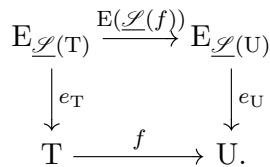
\includegraphics[keepaspectratio]{images/part001_16180f76.jpg}}
\end{enumerate}

This follows from I, p.~54, formula (2) for the first, and it is an immediate consequence of the definitions for the second. This implies that for every pair \((\mathcal{F},\mathcal{G})\) of sheaves on B and every pair (T,U) of étale B-spaces, the maps \(\varphi\mapsto\mathrm{E}(\varphi)\) and \(f\mapsto\underline{\mathcal{L}}(f)\) considered above are bijective.

These results make it possible to deduce a statement about étale B-spaces from a statement about sheaves on B, and conversely.

\subsection{Direct image and inverse image of a sheaf}

Let A and B be topological spaces and \(u: A \rightarrow B\) a continuous map.

Let \(\mathcal{F} = (\mathcal{F}(\mathrm{U}), f_{\mathrm{UV}})\) be a presheaf on A. We define a presheaf \(\mathcal{F}'\) on B as follows: for every open set U of B, set \(\mathcal{F}'(\mathrm{U}) = \mathcal{F}(u^{-1}(\mathrm{U}))\) and for every pair (U, V) of open sets of B such that U \(\subset\) V, set \(f_{\mathrm{UV}}' = f_{u^{-1}(\mathrm{U})u^{-1}(\mathrm{V})}\) . Then \((\mathcal{F}'(\mathrm{U}), f_{\mathrm{UV}}')\) is a presheaf on B. We denote it by \(u_{*}(\mathcal{F})\) and call it the direct image presheaf of the presheaf \(\mathcal{F}\) under the map u.

If \((\mathrm{U}_{i})_{i\in\mathrm{I}}\) is a family of open sets of B, we have \(u^{-1}(\bigcup_{i\in\mathrm{I}}\mathrm{U}_{i})=\bigcup_{i\in\mathrm{I}}u^{-1}(\mathrm{U}_{i})\) and \(u^{-1}(\bigcap_{i\in\mathrm{I}}\mathrm{U}_{i})=\bigcap_{i\in\mathrm{I}}u^{-1}(\mathrm{U}_{i})\) (E, II, p.~25, prop. 3 and 4). It follows immediately that if F has property \((\mathrm{F}_{1})\) (resp. \((\mathrm{F}_{2})\) ) of sheaves (I, p.~43), then so does \(u_{*}(\mathcal{F})\) . Consequently, the direct image of a sheaf is a sheaf.

Let \(\mathcal{F}_1\) and \(\mathcal{F}_2\) be presheaves on A and let \(\varphi\colon\mathcal{F}_1\to\mathcal{F}_2\) be a morphism of presheaves. There then exists a unique morphism of presheaves \(u_*\varphi\colon u_*\mathcal{F}_1\to u_*\mathcal{F}_2\) such that for every open set U of B, the map \((u_*\varphi)(U)\colon(u_*\mathcal{F}_1)(U)\to(u_*\mathcal{F}_2)(U)\) is the map \(\varphi(u^{-1}(U))\colon\mathcal{F}_{1}(u^{-1}(U))\to\mathcal{F}_{2}(u^{-1}(U)).\) If \(\mathcal{F}_{3}\) is a presheaf on A and if \(\psi\colon\mathcal{F}_{2}\to\mathcal{F}_{3}\) is a morphism of presheaves, we have \(u_{*}(\psi\circ\varphi)=u_{*}(\psi)\circ u_{*}(\varphi)\) .

Let C be a topological space and let \(v: B \to C\) be a continuous map. If \(\mathcal{F}\) is a presheaf on A, the presheaves \(v_{*}(u_{*}(\mathcal{F}))\) and \((v \circ u)_{*}(\mathcal{F})\) coincide. If \(\varphi: \mathcal{F}_{1} \to \mathcal{F}_{2}\) is a morphism of presheaves on A, we have the equality \(v_{*}(u_{*}(\varphi)) = (v \circ u)_{*}(\varphi)\) .

Example 1. --- Let B be a topological space, A a subspace of B, and \(\mathcal{F} = (\mathcal{F}(U), f_{\mathrm{UV}})\) a presheaf on A. Denote by \(i: A \to B\) the canonical injection. We then have \(i_*(\mathcal{F}) = (\mathcal{F}'(U), f_{\mathrm{UV}}')\) where for every open set U of B, \(\mathcal{F}'(U) = \mathcal{F}(U \cap A)\) , and for every pair (U, V) of open sets of B with \(U \subset V\) , \(f_{\mathrm{UV}}' = f_{(\mathrm{U} \cap A)(\mathrm{V} \cap A)}\) .

Now let \(\mathcal{G}\) be a presheaf on B. We define the inverse image of the presheaf \(\mathcal{G}\) under \(u\) , and denote by \(u^{*}(\mathcal{G})\) the sheaf \(\underline{\mathcal{C}}_{\mathrm{B}}(\mathrm{A};\mathrm{E}_{\mathcal{G}})\) on A of B-morphisms with values in the B-space \(\mathrm{E}_{\mathcal{G}}\) (I, p.~45, example 4). It is canonically isomorphic to the sheaf on A of sections of the A-étale space \(\mathrm{A} \times_{\mathrm{B}} \mathrm{E}_{\mathcal{G}}\) (I, p.~9, prop. 3). From this we deduce (I, p.~52, example 2) a canonical isomorphism \(\varphi\) of the étale space associated with \(u^{*}(\mathcal{G})\) onto the A-space \(\mathrm{A} \times_{\mathrm{B}} \mathrm{E}_{\mathcal{G}}\) . If moreover \(\mathcal{G}\) is a sheaf, then for every point \(a\) of A there is a canonical bijection \(\psi_{a}: u^{*}(\mathcal{G})_{a} \to \mathcal{G}_{u(a)}\) : for every open neighborhood U of \(a\) in A and every B-morphism \(f: \mathrm{U} \to \mathrm{E}_{\mathcal{G}}\) , we have

\[
\varphi ([ \mathrm{U}, f, a ]) = (a, f (a)), \quad \psi_ {a} ([ \mathrm{U}, f, a ]) = f (a).
\]

Let \(\mathcal{G}_1\) and \(\mathcal{G}_2\) be presheaves on B and \(\varphi\colon\mathcal{G}_1\to\mathcal{G}_2\) a morphism of presheaves. By base change of the morphism of B-étale spaces \(\mathrm{E}(\varphi)\colon\mathrm{E}_{\mathcal{G}_1}\to\mathrm{E}_{\mathcal{G}_2}\) we deduce a morphism of A-étale spaces \(\mathrm{A}\times_{\mathrm{B}}\mathrm{E}_{\mathcal{G}_1}\to\mathrm{A}\times_{\mathrm{B}}\mathrm{E}_{\mathcal{G}_2}\) , whence a morphism of sheaves on A, \(u^{*}(\varphi)\colon u^{*}(\mathcal{G}_{1})\to u^{*}(\mathcal{G}_{2})\) . Let \(\mathcal{G}_3\) be a presheaf on B and \(\psi\colon\mathcal{G}_2\to\mathcal{G}_3\) a morphism of presheaves. We then have the equality \(u^{*}(\psi\circ\varphi)=u^{*}(\psi)\circ u^{*}(\varphi)\) .

Let C be a topological space and let \(v\colon B \to C\) be a continuous map. If \(\mathcal{G}\) is a presheaf on C, the sheaves \(u^{*}(v^{*}(\mathcal{G}))\) and \((v \circ u)^{*}(\mathcal{G})\) are canonically identified (I, p.~5). If \(\varphi\colon\mathcal{G}_{1} \to \mathcal{G}_{2}\) is a morphism of presheaves on C, we moreover have \(u^{*}(v^{*}(\varphi)) = (v \circ u)^{*}(\varphi)\) .

Remark. --- The canonical morphism \(\sigma_{\mathcal{G}}\colon\mathcal{G}\to\widetilde{\mathcal{G}}\) of I, p.~53 corresponds in terms of étale spaces to the isomorphism \(j_{\mathcal{G}}\) of Proposition 2 of I, p.~53. It follows that \(u^{*}(\sigma_{\mathcal{G}})\) is an isomorphism. In particular, if \(A = B\) and \(u = \mathrm{Id}_A\) , the presheaf \(u^{*}(\mathcal{F})\) is the sheaf \(\widetilde{\mathcal{F}}\) .

Example 2. --- Let B be a topological space and A a subspace of B. Denote by \(i\colon\mathrm{A}\to\mathrm{B}\) the canonical injection. For every sheaf \(\mathcal{G}\) on B, denote by \(\mathcal{G}_{\mathrm{A}}\) the sheaf \(i^{*}(\mathcal{G})\) and call \(\mathcal{G}_{\mathrm{A}}\) the sheaf on A induced by the sheaf \(\mathcal{G}\) . The sheaf \(\mathcal{G}_{\mathrm{A}}\) is identified with the sheaf \(\underline{\mathcal{L}}(\mathrm{A};(\mathrm{E}_{\mathcal{G}})_{\mathrm{A}})\) of sections of the A-étale space induced by \(\mathrm{E}_{\mathcal{G}}\) over A.

Suppose that A is an open subspace of B, and let \(\mathcal{G}\) be a sheaf on B. By definition, the sheaf \(\mathcal{G}_{\mathrm{A}}\) is the sheaf \(\widetilde{\mathcal{G}}\mid \mathrm{A}\) deduced from \(\widetilde{\mathcal{G}}\) by restriction to the open set A (I, p.~43). Let \(\sigma_{\mathcal{G}}\colon \mathcal{G}\to \widetilde{\mathcal{G}}\) be the canonical isomorphism (I, p.~55, cor. 1). Then \(\sigma_{\mathcal{G}}\mid \mathrm{A}\) is a canonical isomorphism from the sheaf \(\mathcal{G}\mid \mathrm{A}\) onto the sheaf \(\mathcal{G}_{\mathrm{A}}\), called the canonical isomorphism of \(\mathcal{G}\mid \mathrm{A}\) onto \(\mathcal{G}_{\mathrm{A}}\) .

\subsection{\texorpdfstring{The homomorphisms \(\alpha\) and \(\beta\) ; adjunction}{The homomorphisms alpha and beta ; adjunction}}

Let A and B be topological spaces and let \(u\colon\mathrm{A}\to\mathrm{B}\) be a continuous map. Let \(\mathcal{G}\) be a presheaf on B. By definition of the direct image of presheaves, a section of the sheaf \(u_{*}u^{*}\mathcal{G}\) over an open set U of B is a section of the sheaf \(u^{*}\mathcal{G}\) over the open set \(u^{-1}(\mathrm{U})\) of A, that is, a B-morphism \(u^{-1}(\mathrm{U})\to\mathrm{E}_{\mathcal{G}}\) . One thus defines a morphism of sheaves \(\widetilde{\mathcal{G}}\to u_{*}u^{*}\mathcal{G}\) by associating to the section \(s\) of \(\mathrm{E}_{\mathcal{G}}\) over an open set U of B the section \(s\circ u\) of \(\mathrm{E}_{\mathcal{G}}\) over \(u^{-1}(\mathrm{U})\) . The composition of this morphism and the canonical morphism \(\sigma_{\mathcal{G}}\colon\mathcal{G}\to\widetilde{\mathcal{G}}\) (I, p.~53) is a morphism of presheaves \(\mathcal{G}\to u_{*}u^{*}\mathcal{G}\) which will be denoted by \(\beta_{\mathcal{G}}^{u}\) , or even \(\beta_{\mathcal{G}}\) if there is no ambiguity about the map \(u\) .

Remarks. --- 1) Let A, B, C be topological spaces, let \(u\colon A \to B\) , \(v\colon B \to C\) be continuous maps; set \(w = v \circ u\) . Let \(\mathcal{G}\) be a presheaf on C.

Let U be an open set of C and let s be a section of \(E_{G}\) over U. Then \(\beta_{\mathcal{G}}^{v}(s)\) is the section \(s \circ v\) of \(E_{G}\) over \(v^{-1}(U)\) , and \(v_{*}(\beta_{v^{*}\mathcal{G}}^{u})(\beta_{\mathcal{G}}^{v}(s))\) is the section \(s \circ v \circ u = s \circ w\) of \(E_{G}\) over \(u^{-1}(v^{-1}(U)) = w^{-1}(U)\) .

It follows that \(\beta_{\mathcal{G}}^{w} = v_{*}(\beta_{v^{*}\mathcal{G}}^{u})\circ \beta_{\mathcal{G}}^{v}\) .

\begin{enumerate}
\def\labelenumi{\arabic{enumi})}
\setcounter{enumi}{1}
\tightlist
\item
  If \(\gamma\colon\mathcal{G}_{1}\to\mathcal{G}_{2}\) is a morphism of presheaves on B, the morphisms of presheaves \(\beta_{\mathcal{G}_{2}}\circ\gamma\) and \(u_{*}u^{*}(\gamma)\circ\beta_{\mathcal{G}_{1}}\) are equal. Indeed, if V is an open set of B and \(s\in\mathcal{G}_{1}(V)\) , \(\beta_{\mathcal{G}_{1}}(s)\) is the section \(t\) of A \(\times_{B}E_{\mathcal{G}_{1}}\) over \(u^{-1}(V)\) , defined by \(x\mapsto(x,[V,s,u(x)])\) . The image of \(t\) under \(u^{*}(\gamma)\) is thus the section of A \(\times_{B}E_{\mathcal{G}_{2}}\) over \(u^{-1}(V)\) given by \(x\mapsto(x,[V,\gamma(s),u(x)])\) . It follows that \(u_{*}u^{*}(\gamma)\circ\beta_{\mathcal{G}_{1}}(s)=\beta_{\mathcal{G}_{2}}(\gamma(s))\) .
\end{enumerate}

PROPOSITION 4. --- Let A and B be topological spaces, let \(u\colon A\to B\) be a continuous map, let \(\mathcal{G}\) be a presheaf on B, and let \(\mathcal{F}\) be a sheaf on A.

For every morphism of presheaves \(\varphi\colon\mathcal{G}\to u_{*}\mathcal{F}\) , there exists a unique morphism of sheaves \(\psi\colon u^{*}(\mathcal{G})\to\mathcal{F}\) such that \(\varphi=u_{*}(\psi)\circ\beta_{\mathcal{G}}\) .

In other words, the canonical map

\[
\operatorname{Mor} \left(u ^ {*} (\mathcal {G}), \mathcal {F}\right)\rightarrow \operatorname{Mor} \left(\mathcal {G}, u _ {*} (\mathcal {F})\right), \quad \psi \mapsto u _ {*} (\psi) \circ \beta_ {\mathcal {G}}
\]

is a bijection.

Using the notation of Proposition 4, we will sometimes denote \(\psi = \varphi^{\sharp}\) and \(\varphi = \psi^{\flat}\) .

Let us prove Proposition 4. By Remark 2 applied to the morphism \(\sigma_{\mathcal{G}}: \mathcal{G} \to \widetilde{\mathcal{G}}\) , the morphism \(\beta_{\mathcal{G}}\) is equal to the composition

\[
u _ {*} (u ^ {*} (\sigma_ {\mathcal {G}}) ^ {- 1}) \circ \beta_ {\widetilde {\mathcal {G}}} \circ \sigma_ {\mathcal {G}},
\]

where \(u^{*}(\sigma_{\mathcal{G}}) \colon u^{*}(\mathcal{G}) \to u^{*}(\widetilde{\mathcal{G}})\) is the canonical isomorphism of Remark I, p.~58. Let \(\widetilde{\varphi} \colon \widetilde{\mathcal{G}} \to u_{*}\mathcal{F}\) be the unique morphism of sheaves such that \(\widetilde{\varphi} \circ \sigma_{\mathcal{G}} = \varphi\) (I, p.~54, prop. 3). It then suffices to show that there exists a unique morphism of sheaves \(\widetilde{\psi} \colon u^{*}(\mathcal{G}) \to \mathcal{F}\) such that \(u_{*}(\widetilde{\psi}) \circ \beta_{\widetilde{\mathcal{G}}} = \widetilde{\varphi}\) .

We may therefore assume that \(\mathcal{G}\) is a sheaf. For a morphism of sheaves \(\psi: u^{*}(\mathcal{G}) \to \mathcal{F}\) to satisfy the conclusion of Proposition 4, it is necessary and sufficient that for every open set V of B and every section \(t\) of \(\mathrm{E}_{\mathcal{G}}\) above V, one has

\[
\varphi_{\mathrm{V}}(t) = \psi_{u^{-1}(\mathrm{V})}(t \circ u \mid u^{-1}(\mathrm{V})).\tag{6}
\]

Let \(U_{0}\) be an open subset of A and \(s_{0}\) be an element of \(u^{*}(\mathcal{G})(\mathrm{U}_{0})\), in other words, a B-morphism from \(U_{0}\) into \(E_{\mathcal{G}}\) . Let \(\mathrm{S}(\mathrm{U}_{0}, s_{0})\) be the set of triples \((\mathrm{U}, \mathrm{V}, t)\) where U is an open subset of A contained in \(U_{0}\) , V is an open subset of B such that \(u(\mathrm{U}) \subset \mathrm{V}\), and let t be a section of \(E_{\mathcal{G}}\) above V such that one has

\[
t \circ u \mid \mathrm{U} = s _ {0} \mid \mathrm{U}.\tag{7}
\]

If \(U_{1}\) and \(U_{2}\) are open subsets of A with \(U_{1} \subset U_{2}\) , denote by \(f_{U_{1}U_{2}}\) the restriction map \(\mathcal{F}(U_{2}) \to \mathcal{F}(U_{1})\) . For every \((\mathrm{U}, \mathrm{V}, t) \in \mathrm{S}(\mathrm{U}_{0}, s_{0})\) we then have the relation

\[
\begin{array}{l} f_{\mathrm{U}\mathrm{U}_{0}}(\psi_{\mathrm{U}_{0}}(s_{0})) = \psi_{\mathrm{U}}(s_{0} \mid \mathrm{U}) \\ \qquad = \psi_{\mathrm{U}}(t \circ u \mid \mathrm{U}) \\ \qquad = f_{\mathrm{U}u^{-1}(\mathrm{V})}(\psi_{u^{-1}(\mathrm{V})}(t \circ u \mid u^{-1}(\mathrm{V}))). \end{array}
\]

Consequently, if \(\psi \colon u^{*}(\mathcal{G})\to \mathcal{F}\) satisfies (6), we have

\[
f_{\mathrm{U}\mathrm{U}_{0}}(\psi_{\mathrm{U}_{0}}(s_{0})) = f_{\mathrm{U}u^{-1}(\mathrm{V})}(\varphi_{\mathrm{V}}(t)).\tag{8}
\]

Let us prove that, for every point \(a\) of \(\mathrm{U}_0\) , there exists a triple \((\mathrm{U},\mathrm{V},t)\in \mathrm{S}(\mathrm{U}_0,s_0)\) such that \(a\in \mathrm{U}\). Indeed, let \(a\) be a point of \(\mathrm{U}_0\). There exists an open neighborhood V in B containing \(u(a)\) and a section \(t\) of the étale space \(\mathbf{E}_{\mathcal{G}}\) over V such that \(t(u(a)) = s_0(a)\) (I, p.~33, prop. 9). Let \(\mathrm{U}_1 = u^{-1} (\mathrm{V})\cap \mathrm{U}_0\) . The sections \(s_0\mid \mathrm{U}_1\) and \(t\circ u\mid \mathrm{U}_1\) of the étale space over \(\mathrm{U}_1\), \(\mathbf{E}_{\mathcal{G}}\times_{\mathrm{B}}\mathrm{U}_1\), coincide at the point \(a\). By Proposition 11, b) of I, p.~34, the set of points where they coincide is an open set U of \(\mathrm{U}_1\) which contains \(a\). The triple \((\mathrm{U},\mathrm{V},t)\) then belongs to \(\mathrm{S}(\mathrm{U}_0,s_0)\) .

Formula (8) and the property \((\mathrm{F}_{1})\) of sheaves (I, p.~43) then imply the uniqueness of \(\psi\) .

Let (U, V, t) and \((\mathrm{U}^{\prime}, \mathrm{V}^{\prime}, t^{\prime})\) be elements of \(\mathrm{S}(\mathrm{U}_{0}, s_{0})\) . By relation (7), the restrictions of t and \(t^{\prime}\) to \(u(\mathrm{U} \cap \mathrm{U}^{\prime})\) coincide. By prop. 11, b) of I, p.~34, there exists an open set W of B such that \(u(\mathrm{U} \cap \mathrm{U}^{\prime}) \subset \mathrm{W} \subset \mathrm{V} \cap \mathrm{V}^{\prime}\) and that \(t \mid W = t^{\prime} \mid W\) . We therefore have

\[
f_{u^{-1}(\mathrm{W})u^{-1}(\mathrm{V})}(\varphi_{\mathrm{V}}(t)) = \varphi_{\mathrm{W}}(t\mid \mathrm{W}) = \varphi_{\mathrm{W}}(t^{\prime}\mid \mathrm{W}) = f_{u^{-1}(\mathrm{W})u^{-1}(\mathrm{V}^{\prime})}(\varphi_{\mathrm{V}^{\prime}}(t^{\prime}))
\]

whence

\[
f_{(\mathrm{U}\cap\mathrm{U}^{\prime})u^{-1}(\mathrm{V})}(\varphi_{\mathrm{V}}(t)) = f_{(\mathrm{U}\cap\mathrm{U}^{\prime})u^{-1}(\mathrm{V}^{\prime})}(\varphi_{\mathrm{V}^{\prime}}(t^{\prime})).\tag{9}
\]

By the properties \((\mathrm{F}_{1})\) and \((\mathrm{F}_{2})\) for the sheaf F, there exists a unique element \(s'\) of \(\mathcal{F}(\mathrm{U}_{0})\) such that for every triple \((\mathrm{U},\mathrm{V},t)\) of

\(\mathrm{S}(\mathrm{U}_{0},s_{0})\) one has:

\[
f_{\mathrm{U}\mathrm{U}_{0}}(s^{\prime}) = f_{\mathrm{U}u^{-1}(\mathrm{V})}(\varphi_{\mathrm{V}}(t)).\tag{10}
\]

Denote by \(\psi_{\mathrm{U}_{0}}(s_{0})\) this element.

Let \(U_{1}\) be an open set contained in \(U_{0}\) and let \(s_{1}=s_{0}|U_{1}\) . If \((\mathrm{U},\mathrm{V},t)\in\mathrm{S}(\mathrm{U}_{1},s_{1})\) , then U is an open set contained in \(U_{0}\) and \(t\circ u|U=s_{1}|U=s_{0}|U\) , therefore \((\mathrm{U},\mathrm{V},t)\in\mathrm{S}(\mathrm{U}_{0},s_{0})\) , and relation (10) then implies that

\[
f_{\mathrm{U}\mathrm{U}_{1}}(f_{\mathrm{U}_{1}\mathrm{U}_{0}}(\psi_{\mathrm{U}_{0}}(s_{0}))) = f_{\mathrm{U}\mathrm{U}_{0}}(\psi_{\mathrm{U}_{0}}(s_{0})) = f_{\mathrm{U}u^{-1}(\mathrm{V})}(\varphi_{\mathrm{V}}(t)).
\]

By definition of \(\psi_{\mathrm{U}_{1}}(s_{1})\) , we therefore have \(\psi_{\mathrm{U}_{1}}(s_{1}) = f_{\mathrm{U}_{1}\mathrm{U}_{0}}(\psi_{\mathrm{U}_{0}}(s_{0}))\) . This proves that the family \(\psi = (\psi_{\mathrm{U}})\) is a morphism of sheaves from \(u^{*}(\mathcal{G})\) into \(\mathcal{F}\).

Let us prove that \(\psi\) satisfies relation (6). Let V be an open subset of B and \(t\) be a section of \(\mathrm{E}_{\mathcal{G}}\) above V. If \(\mathrm{U} = u^{-1}(\mathrm{V})\) and if \(s = t \circ u \mid \mathrm{U}\) , the triple \((\mathrm{U}, \mathrm{V}, t)\) belongs to \(\mathrm{S}(\mathrm{U}, s)\) and relation (6) is an immediate consequence of relation (10), applied to \(\mathrm{U} = \mathrm{U}_0\) .

PROPOSITION 5. — Let A and B be topological spaces and let u: A → B be a continuous map.

\begin{enumerate}
\def\labelenumi{\alph{enumi})}
\tightlist
\item
  Let \(\mathcal{G}_1\) and \(\mathcal{G}_2\) be presheaves on B and let \(\gamma\colon\mathcal{G}_1\to\mathcal{G}_2\) be a morphism of presheaves. Let also \(\mathcal{F}\) be a sheaf on A and \(\varphi\colon\mathcal{G}_2\to u_*\mathcal{F}\) a morphism of presheaves. We have the equality
\end{enumerate}

\[
(\varphi \circ \gamma) ^ {\sharp} = \varphi^ {\sharp} \circ u ^ {*} (\gamma).\tag{11}
\]

\begin{enumerate}
\def\labelenumi{\alph{enumi})}
\setcounter{enumi}{1}
\tightlist
\item
  Let \(\mathcal{F}_1\) and \(\mathcal{F}_2\) be sheaves on A and let \(\mathcal{G}\) be a presheaf on B. Let \(\varphi\colon\mathcal{F}_1\to\mathcal{F}_2\) be a morphism of sheaves and let \(\gamma\colon\mathcal{G}\to u_*\mathcal{F}_1\) be a morphism of presheaves. We have the relation
\end{enumerate}

\[
(u _ {*} (\varphi) \circ \gamma) ^ {\sharp} = \varphi \circ \gamma^ {\sharp}.
\]

\begin{enumerate}
\def\labelenumi{\alph{enumi})}
\tightlist
\item
  By definition of \(\varphi^{\sharp}\) and Remark 2 of I, p.~60, we have
\end{enumerate}

\[
\varphi \circ \gamma = u _ {*} (\varphi^ {\sharp}) \circ \beta_ {\mathcal {G} _ {2}} \circ \gamma = u _ {*} (\varphi^ {\sharp}) \circ u _ {*} u ^ {*} (\gamma) \circ \beta_ {\mathcal {G} _ {1}}.
\]

Therefore, \(\varphi \circ \gamma = u_{*}(\varphi^{\sharp}\circ u^{*}(\gamma))\circ \beta_{\mathcal{G}_{1}}\); whence relation (11).

\begin{enumerate}
\def\labelenumi{\alph{enumi})}
\setcounter{enumi}{1}
\tightlist
\item
  By definition of \(\gamma^{\sharp}\) , we have
\end{enumerate}

\[
u _ {*} (\varphi) \circ \gamma = u _ {*} (\varphi) \circ u _ {*} (\gamma^ {\sharp}) \circ \beta_ {\mathcal {G}} = u _ {*} (\varphi \circ \gamma^ {\sharp}) \circ \beta_ {\mathcal {G}},
\]

whence the announced relation, taking into account the definition of \((u_{*}(\varphi)\circ\gamma)^{\sharp}\) .

Set \(\alpha_{\mathcal{F}} = \mathrm{Id}_{u_*(\mathcal{F})}^\sharp\) ; it is the unique morphism of sheaves \(\rho \colon u^*(u_*(\mathcal{F})) \to \mathcal{F}\) such that

\[
\operatorname{Id} _ {u _ {*} (\mathcal {F})} = u _ {*} (\rho) \circ \beta_ {u _ {*} (\mathcal {F})}.
\]

Relation (11) applied to \(\mathcal{G}_2 = u_*(\mathcal{F})\) and to the morphism \(\varphi = \mathrm{Id}_{u_*(\mathcal{F})}\) yields, for every morphism of presheaves \(\gamma\colon\mathcal{G}\to u_*(\mathcal{F})\), the factorization

\[
\gamma^ {\sharp} = \alpha_ {\mathcal {F}} \circ u ^ {*} (\gamma).
\]

It then follows from Proposition 4 that for every morphism of sheaves \(\psi\) from \(u^{*}(\mathcal{G})\) into \(\mathcal{F}\) , \(\psi^{\flat}\) is the unique morphism \(\varphi\colon\mathcal{G}\to u_{*}(\mathcal{F})\) such that \(\psi=\alpha_{\mathcal{F}}\circ u^{*}(\varphi)\) .

Examples. --- 1) Consider a topological space B, a subspace A of B, and denote by \(i\colon A \to B\) the canonical injection. Let \((E,p)\) and \((E',p')\) be B-spaces. Take for \(\mathcal{G}\) the sheaf \(\underline{\mathcal{M}or}_{B}(E;E')\) (I, p.~45, Example 4) and for \(\mathcal{F}\) the sheaf \(\underline{\mathcal{M}or}_{A}(E_{A};E_{A}')\) . For every open set V of B and every V-morphism \(f\colon E_{V} \to E_{V}'\) , set \(\varphi_{V}(f) = f_{V \cap A}\) , where \(f_{V \cap A}\) is the \((V \cap A)\) -morphism from \(E_{V \cap A}\) into \(E_{V \cap A}'\) induced by \(f\) . The family \(\varphi = (\varphi_{V})\) thus defined is a morphism of sheaves from \(\mathcal{G}\) into \(i_*\mathcal{F}\) . By Proposition 4, there exists a unique morphism of sheaves \(\psi\colon \underline{\mathcal{M}or}_{B}(E;E')_{A} \to \underline{\mathcal{M}or}_{A}(E_{A};E_{A}')\) such that one has

\[
\psi_ {\mathrm{V} \cap \mathrm{A}} (\sigma_ {\mathcal {G}} (\mathrm{V}, f) \mid \mathrm{V} \cap \mathrm{A}) = f _ {\mathrm{V} \cap \mathrm{A}}\tag{12}
\]

for every open set V of B and every \(f \in \mathcal{C}_{\mathrm{V}}(\mathrm{E}_{\mathrm{V}}; \mathrm{E}_{\mathrm{V}}^{\prime})\) . The morphism \(\psi\) is called the canonical morphism from \(\underline{\mathcal{M}or_{B}}(\mathrm{E}; \mathrm{E}^{\prime})_{\mathrm{A}}\) into \(\underline{\mathcal{M}or_{A}}(\mathrm{E}_{\mathrm{A}}; \mathrm{E}_{\mathrm{A}}^{\prime})\) .

If A is reduced to a single point \(a\) , this morphism is identified with the morphism from the stalk at \(a\) of the sheaf \(\underline{\mathcal{M}or}_{\mathrm{B}}(\mathrm{E};\mathrm{E}^{\prime})\) into the set \(\mathcal{C}(\mathrm{E}_a;\mathrm{E}_a')\) .

By passing to subsheaves, the morphism \(\psi\) induces a canonical morphism of \(\mathcal{I}som_{\mathrm{B}}(\mathrm{E};\mathrm{E}')_{\mathrm{A}}\) into \(\mathcal{I}som_{\mathrm{A}}(\mathrm{E}_{\mathrm{A}};\mathrm{E}_{\mathrm{A}}^{\prime})\) .

\begin{enumerate}
\def\labelenumi{\arabic{enumi})}
\setcounter{enumi}{1}
\tightlist
\item
  Let A, B, C be topological spaces and let \(u\colon A\to B\) , \(v\colon B\to C\) be continuous maps; set \(w=v\circ u\) . Let E and E' be C-spaces. The canonical morphism of \(\underline{\mathcal{M}or}_{C}(E;E')_{A}\) into \(\underline{\mathcal{M}or}_{A}(E_{A};E'_{A})\) is the composite of the morphism \(\underline{\mathcal{M}or}_{C}(E;E')_{A}\to\underline{\mathcal{M}or}_{B}(E_{B};E'_{B})_{A}\) deduced from the canonical morphism of \(\underline{\mathcal{M}or}_{C}(E;E')_{B}\) into \(\underline{\mathcal{M}or}_{B}(E_{B};E'_{B})\) and the canonical morphism of \(\underline{\mathcal{M}or}_{B}(E_{B},E'_{B})_{A}\) into \(\underline{\mathcal{M}or}_{A}(E_{A},E'_{A})\) .
\end{enumerate}
% semantic-fragments: legacy-input-seam
\relax{}
\subsection{Soft sheaves}

DEFINITION 5. --- Let \(p\colon E \rightarrow B\) be an étale map. One says that the map \(p\) is soft, or that the étale B-space \((E,p)\) is soft, if every continuous section of \(p\) over a closed subspace of B extends to a continuous section of \(p\) over B.

Let F be a sheaf on B. One says that F is a soft sheaf if the associated étale space (I, p. 50, def. 4) is soft.

Let \(\mathcal{F}\) be a sheaf on B. The sheaf \(\mathcal{F}\) is soft if and only if for every closed set Z of B, every open neighborhood U of Z, and every \(s \in \mathcal{F}(\mathrm{U})\) , there exists \(t \in \mathcal{F}(\mathrm{B})\) and an open neighborhood V of Z contained in U such that \(s \mid \mathrm{V} = t \mid \mathrm{V}\) .

If \(\mathcal{F}\) is a soft sheaf, \(\mathcal{F}(\mathrm{B})\) is nonempty: indeed, the unique section of the étale space \(\mathrm{E}_{\mathcal{F}}\) associated with \(\mathcal{F}\) over \(\varnothing\) extends to a continuous section of \(\mathrm{E}_{\mathcal{F}}\) over B.

Let \(p \colon \mathrm{E} \to \mathrm{B}\) be an étale map and let A be a closed subspace of B. If \(p\) is soft, the map \(p_{\mathrm{A}} \colon \overline{p}^{1}(\mathrm{A}) \to \mathrm{A}\) is soft. Equivalently, if \(\mathcal{F}\) is a soft sheaf on B, the sheaf induced on a closed subspace A is soft.

PROPOSITION 6. --- Let B be a topological space, let \(\mathcal{F}\) be a sheaf on B, and let \((\mathrm{A}_i)_{i\in \mathrm{I}}\) be a locally finite closed covering of B. The sheaf \(\mathcal{F}\) is soft if and only if, for every \(i\in \mathrm{I}\), the induced sheaf \(\mathcal{F}_{\mathrm{A}_i}\) is soft.

The condition is evidently necessary. Let us prove that it is sufficient. Denote by \(p\colon \mathrm{E}\to \mathrm{B}\) the B-étale space \(\mathrm{E}_{\mathcal{F}}\) associated with the sheaf \(\mathcal{F}\) . Let A be a closed subspace of B and \(s\colon \mathrm{A}\to \mathrm{E}\) a continuous section of \(p\) over A; it must be shown that \(s\) has a continuous extension to B. For every subset J of I, set \(\mathrm{A_J} = \bigcup_{i\in \mathrm{J}}\mathrm{A}_i\) ; the set \(\mathrm{A_J}\) is closed in B (TG, I, p. 6, prop. 4).

Let \(\mathcal{S}\) be the set of pairs \((\mathrm{J},t)\) where \(\mathrm{J}\) is a subset of I and \(t\) is a continuous section of E over \(\mathrm{A_J}\) which coincides with \(s\) on \(\mathrm{A} \cap \mathrm{A_J}\) . Equip \(\mathcal{S}\) with the order relation denoted \(\leqslant\) for which \((\mathrm{J},t) \leqslant (\mathrm{J}',t')\) if \(\mathrm{J} \subset \mathrm{J}'\) and \(t' \mid \mathrm{A_J} = t\) . For \(\sigma = (\mathrm{J},t) \in \mathcal{S}\) , write \(\mathrm{J}_{\sigma} = \mathrm{J}\) and \(t_{\sigma} = t\) . Let us show that the ordered set \(\mathcal{S}\) is inductive. Let S be a totally ordered subset of \(\mathcal{S}\) . Set \(\mathrm{J} = \bigcup_{\sigma \in \mathrm{S}} \mathrm{J}_{\sigma}\) ; this is a subset of I. One then defines a section \(t\) of E over \(\mathrm{A_J}\) by setting \(t(x) = t_{\sigma}(x)\) , if \(x \in \mathrm{A}_{J_{\sigma}}\) ; one therefore has \(t \mid \mathrm{A} \cap \mathrm{A_J} = s\) . Let \(j \in \mathrm{J}\) and let \(\sigma \in S\) such that \(j \in J_{\sigma}\) ; since \(t \mid A_j = t_{\sigma} \mid A_j\) the restriction of \(t\) to \(A_j\) is continuous. It then follows from TG, I, p. 19, prop. 4 that \(t\) is continuous. Thus, (J, t) is an element of \(\mathcal{S}\) ; by construction, it is an upper bound of S. This proves that the set \(\mathcal{S}\) is inductive. It therefore possesses a maximal element (J, t) (E, III, p. 20, th. 2).

Let us argue by contradiction, assuming that \(J \neq I\) . Let i be an element of \(I \setminus J\). Set \(A' = (A_i \cap A) \cup (A_i \cap A_J)\) and define a section \(s'\) of E over \(A'\) by:

\[
s ^ {\prime} (a) = \left\{ \begin{array}{l l} s (a) & \text {for} a \in \mathrm{A} _ {i} \cap \mathrm{A}, \\ t (a) & \text {for} a \in \mathrm{A} _ {i} \cap \mathrm{A} _ {\mathrm{J}}, \end{array} \right.
\]

which is possible since \(s\) and \(t\) coincide on \(\mathrm{A} \cap \mathrm{A}_{\mathrm{J}}\) . Moreover, since \(\mathrm{A}_{i} \cap \mathrm{A}\) and \(\mathrm{A}_{i} \cap \mathrm{A}_{\mathrm{J}}\) are closed, the section \(s'\) is continuous (TG, I, p. 19, prop. 4). By hypothesis, there exists a continuous section \(s_{i}: \mathrm{A}_{i} \to \mathrm{E}\) extending \(s'\) . Since the restrictions of \(s_{i}\) and \(t\) to \(\mathrm{A}_{\mathrm{J}} \cap \mathrm{A}_{i}\) are equal, the map \(t': \mathrm{A}_{\mathrm{J} \cup \{i\}} \to \mathrm{E}\) which coincides with \(t\) on \(\mathrm{A}_{\mathrm{J}}\) and with \(s_{i}\) on \(\mathrm{A}_{i}\) is a continuous section of \(p\) over \(\mathrm{A}_{\mathrm{J} \cup \{i\}}\) , extending \(s| \mathrm{A} \cap \mathrm{A}_{\mathrm{J} \cup \{i\}}\) . One then has \((\mathrm{J}, t) < (\mathrm{J} \cup \{i\}, t')\) , which contradicts the hypothesis that \((\mathrm{J}, t)\) is maximal.

Thus, J = I, hence \(A_{J} = B\) and t is a continuous section of E over B extending s.

COROLLARY 1. --- Let B be a paracompact space, \(\mathcal{F}\) a sheaf on B, and \((\mathrm{U}_i)_{i\in \mathrm{I}}\) an open covering of B. If, for every \(i\in \mathrm{I}\) , the induced sheaf \(\mathcal{F}|\mathrm{U}_i\) is soft, then the sheaf \(\mathcal{F}\) is soft.

Indeed, there exists a locally finite closed covering \((\mathrm{F}_{j})_{j\in\mathrm{J}}\) finer than the covering \((\mathrm{U}_{i})_{i\in\mathrm{I}}\) (TG, IX, p. 49, prop. 4 and p. 48, cor. 1). Consequently, for every \(j\in J\), the sheaf \(\mathcal{F}|F_{j}\) is soft and the proposition implies that the sheaf \(\mathcal{F}\) is soft.

COROLLARY 2. --- Let B be a paracompact space, \(\mathcal{F}\) a sheaf on B, and \((\mathrm{A}_i)_{i\in \mathrm{I}}\) a locally finite closed covering of B. For the sheaf \(\mathcal{F}\) to be soft, it is necessary and sufficient that the following condition be satisfied:

For every \(i \in I\) , every closed subset A of \(A_{i}\) , every open set V of B containing A and every element s of \(\mathcal{F}(V)\) , there exists an open neighborhood U of \(A_{i}\) in B, an element t of \(\mathcal{F}(U)\) and an open neighborhood W of A in B contained in \(U \cap V\) such that \(t | W = s | W\) .

Suppose that the sheaf \(\mathcal{F}\) is soft and let us show that the condition is satisfied. Let \(i\in\mathrm{I}\) , let A be a closed subset of \(\mathrm{A}_{i}\) , let V be an open set of B containing A and let \(s\) be an element of \(\mathcal{F}(\mathrm{V})\) . Set \(s_{0}=\sigma_{\mathcal{F}}(s)\) . It is a continuous section over V of the étale space \(\mathrm{E}_{\mathcal{F}}\) . Since \(\mathrm{A}_{i}\) is closed, A is closed in B and \(s_{0}\mid\mathrm{A}\) extends to a section \(t_{0}\colon\mathrm{B}\to\mathrm{E}_{\mathcal{F}}\) , by definition of a soft sheaf. The sections \(s_{0}\) and \(t_{0}\mid\mathrm{V}\) of the V-étale space \(\mathrm{E}_{\mathcal{F}}\times_{\mathrm{B}}\mathrm{V}\) coincide on A, hence on a neighborhood W of A (I, p. 34, prop. 11, b)).

Conversely, suppose that the condition of the corollary is satisfied. By Proposition 6, it suffices to show that, for every \(i \in I\), the sheaf \(\mathcal{F}_{A_i}\) is soft. Let A be a closed subset of \(A_i\) and let \(s_0\) be a section of the étale space of \(\mathcal{F} | A_i\) over A, that is, a continuous section over A of the étale space \(E_{\mathcal{F}}\) . Since A is closed in B and B is paracompact, \(s_0\) extends to a section \(s\) over a neighborhood V of A in B (I, p. 37, th. 2). By hypothesis, there exists an open neighborhood U of \(A_i\) in B and a section \(t\) of \(E_{\mathcal{F}}\) over U which coincides with \(s\) on a neighborhood of A. The restriction of \(t\) to \(A_i\) is a section of \(\mathcal{F}_{A_i}\) which extends \(s_0\) . The sheaf \(\mathcal{F}_{A_i}\) is therefore soft. By Proposition 6, the sheaf \(\mathcal{F}\) is soft.

\subsection{Structure Sheaves}

Suppose that a species of structure \(\Sigma\) and a notion of \(\sigma\)-morphism relative to this species of structure are given.

Let B be a topological space.

A presheaf \(\mathcal{F}\) on B is said to take values in the species of structure \(\Sigma\) if, for every open set U of B, the set \(\mathcal{F}(\mathrm{U})\) is equipped with a structure of species \(\Sigma\) and the restriction maps are \(\sigma\)-morphisms.

We will say that such a presheaf is a sheaf with values in the species of structure \(\Sigma\) if, moreover, it is a sheaf of sets.

If \(\mathcal{F}\) and \(\mathcal{G}\) are presheaves with values in the species of structure \(\Sigma\), one says that a morphism \(\varphi\) is a morphism of presheaves with values in \(\Sigma\) if, for every open set U, the map \(\varphi(\mathrm{U})\) is a \(\sigma\)-morphism.

One will thus speak, for example, of sheaves of groups, of abelian groups, of \(k\)-modules (for a fixed ring \(k\)), of rings, and of \(k\)-algebras (for a fixed commutative ring \(k\)).

The sheaf on B of maps with values in a group (resp. an abelian group, resp. a \(k\)-module, resp. a ring, resp. a \(k\)-algebra) is naturally endowed with a structure of a sheaf of groups (resp. of abelian groups, resp. of \(k\)-modules, resp. of rings, resp. of \(k\)-algebras). If X is a differentiable manifold of class \(C^{r}\) over R, the sheaf \(\underline{\mathcal{C}}^{r}(\mathrm{X};\mathbf{R})\) of numerical functions of class \(C^{r}\) is a sheaf of R-algebras, and the sheaf on X of sections of class \(C^{r}\) of a vector bundle E over X is a sheaf of R-vector spaces; a differential operator defines a morphism of sheaves of R-vector spaces.

For these species of structure \(\Sigma\), it follows from the construction we have given that the sheaf \(\widetilde{\mathcal{F}}\) associated with a presheaf \(\mathcal{F}\) with values in the species of structure \(\Sigma\) (of groups, of abelian groups, of \(k\)-modules, of rings, of \(k\)-algebras) is a sheaf with values in this kind of structure, and that the canonical morphism \(j_{\mathcal{F}}: \mathcal{F} \to \widetilde{\mathcal{F}}\) is a morphism of presheaves with values in the species of structure \(\Sigma\).

For example, the sheaf on B of maps taking values in a group is naturally endowed with a sheaf-of-groups structure.

Let A and B be topological spaces and let \(u\colon\mathrm{A}\to\mathrm{B}\) be a continuous map. If \(\mathcal{F}\) is a (pre)sheaf on A with values in the species of structure \(\Sigma\), then the same is true of the (pre)sheaf \(u_{*}(\mathcal{F})\), the direct image of the (pre)sheaf \(\mathcal{F}\) under \(u\).

Suppose further that the species of structure \(\Sigma\) is that of groups, abelian groups, \(k\)-modules, rings, or \(k\)-algebras. If \(\mathcal{G}\) is a (pre)sheaf on B with values in the species of structure \(\Sigma\), then the sheaf \(u^{*}\mathcal{G}\) on A, inverse image of the presheaf \(\mathcal{G}\) by the map \(u\), is equipped with a sheaf structure with values in \(\Sigma\). In this case, the adjunction morphisms \(\alpha\) and \(\beta\) are morphisms of presheaves with values in the species of structure \(\Sigma\). In particular, if \(\varphi: \mathcal{G} \to u_{*}\mathcal{F}\) is a morphism of presheaves with values in \(\Sigma\), the same holds for the morphism \(\varphi^{\sharp}\); if \(\psi: u^{*}(\mathcal{G}) \to \mathcal{F}\) is a morphism of presheaves with values in \(\Sigma\), the same holds for the morphism \(\psi^{\flat}\).

\section{COVERINGS}

\subsection{Locally trivial fiber spaces}

Let B be a topological space. If F is a topological space, we call the trivial B-fibered space with fiber type F the B-space \((B \times F, pr_{1})\) .

Let E be a B-space. If there exists a topological space F and a B-isomorphism \(u: E \rightarrow B \times F\), we say that the B-space E is a trivializable B-fibered space and that u is a trivialization of it with fiber type F.

DEFINITION 1. --- Let B be a topological space. Let E be a B-space and let p be its projection. One says that E is a locally trivial B-fibered space if every point of B has a neighborhood V such that \((\overline{p}^{1}(V), p_{V})\) is a trivializable V-fibered space.

Instead of “locally trivial fibered B-space,” one also says “locally trivial fibered space with base B.” If E is a locally trivial fibered B-space, one sometimes says that \((E,B,p)\) is a locally trivial fibration, or, by abuse of language, that p is a locally trivial fibration. One also says that a B-space \((E,p)\) is trivializable over a subset A of B if the A-space \(E_{A}\) induced by \((E,p)\) over A is a trivializable fiber space.

Let E be a locally trivial B-fibered space; denote its projection by p. The set of points a in B for which the fiber \(\overline{p}^{1}(a)\) is empty (resp. nonempty) is open. The image of p is therefore an open and closed subset of B.

Let F be a topological space. If all the fibers of E are homeomorphic to F, then E is said to be a locally trivial B-fibered space with fiber type F.

Remarks. --- 1) Let (E, p) be a locally trivial fiber bundle over B, and let A be a subset of B. The A-space \(\mathrm{E}_{\mathrm{A}} = (\stackrel{-1}{p}(\mathrm{A}), p_{\mathrm{A}})\) deduced from E by passing to subspaces is a locally trivial fiber space. If E is trivializable, then so is \(E_{A}\) .

Indeed, for every point \(a\) of A, there exists an open neighborhood U of \(a\) in B, a topological space F and a U-isomorphism \(g\colon \overline{p}^{1}(\mathrm{U})\to \mathrm{U}\times \mathrm{F}\) . The map \(g\) induces an \((\mathrm{A}\cap \mathrm{U})\) -isomorphism of \(\overline{p}_{\mathrm{A}}^{-1}(\mathrm{A}\cap \mathrm{U})\)

onto \((\mathrm{A}\cap\mathrm{U})\times\mathrm{F}\) , which proves that \(E_{A}\) is a locally trivial fibered A-space.

\begin{enumerate}
\def\labelenumi{\arabic{enumi})}
\setcounter{enumi}{1}
\tightlist
\item
  Let \((\mathrm{E}, p)\) be a B-space and let \((\mathrm{E}_{i})_{i \in \mathrm{I}}\) be a partition of E consisting of open sets.
\end{enumerate}

If each of the B-spaces \((\mathrm{E}_{i}, p \mid \mathrm{E}_{i})\) is a trivializable fiber space, E is a trivializable B-fibered space. Indeed, for each \(i \in I\), let \(F_{i}\) be a topological space such that the B-spaces \((\mathrm{E}_{i}, p \mid \mathrm{E}_{i})\) and \((\mathrm{B} \times \mathrm{F}_{i}, \mathrm{pr}_{1})\) are isomorphic. Then the B-space \((\mathrm{E}, p)\) is isomorphic to \((\mathrm{B} \times \mathrm{F}, \mathrm{pr}_{1})\), where F is the topological sum space of the family \((\mathrm{F}_{i})_{i \in I}\) .

Suppose the set I is finite. If each of the B-spaces \((\mathrm{E}_{i}, p \mid \mathrm{E}_{i})\) is a locally trivial B-fibered space, the same holds for the B-space E. Indeed, since the set I is finite, each point of B has a neighborhood U over which the B-fibered spaces \(E_{i}\) are all trivializable. By the preceding, the U-space \((\bar{p}^{1}(\mathrm{U}), p_{\mathrm{U}})\) is then a trivializable fiber bundle.

\subsection{Coverings}

DEFINITION 2. --- A covering is called a locally trivial fiber space all of whose fibers are discrete.

Instead of saying that a B-space E is a covering, one also says that E is a covering of B.

Let E be a B-space, denote by p its projection; let A be a subset of B. If E is a covering of B, the fibers of p are discrete, hence those of \(p_{\mathrm{A}} \colon \overline{p}^{1}(\mathrm{A}) \to \mathrm{A}\) also, and the locally trivial fibered A-space ( \(\overline{p}^{1}(\mathrm{A}), p_{\mathrm{A}}\) ) is a covering.

PROPOSITION 1. --- Let B and E be topological spaces, and let \(p\colon \mathrm{E}\to \mathrm{B}\) be a map. The following conditions are equivalent:

\begin{enumerate}
\def\labelenumi{(\roman{enumi})}
\item
  The map p is continuous and the B-space (E,p) is a trivializable covering.
\item
  There exists a partition \((\mathrm{V}_{i})_{i\in\mathrm{I}}\) of E consisting of open sets such that, for every \(i\in I\), the map \(p\mid V_{i}\colon V_{i}\to B\) is a homeomorphism.
\end{enumerate}

Suppose that condition (i) is satisfied, and let \(g \colon \mathrm{E} \to \mathrm{B} \times \mathrm{F}\) be a trivialization of the B-space \((\mathrm{E}, p)\), of fiber type F. Consequently, F is a discrete topological space and the sets \(\mathrm{V}_i = g^{-1}(\mathrm{B} \times \{i\})\), for \(i \in F\), form a partition of E consisting of open sets. For every \(i\), the map \(p \mid V_i \colon V_i \to B\) is a homeomorphism, with inverse homeomorphism the map \(x \mapsto g^{-1}(x, i)\), whence condition (ii).

Conversely, suppose that condition (ii) is satisfied. The map p is then continuous. Consider the map from E into \(B \times I\) that sends \(x \in E\) to the pair \((p(x), i)\), where i is the unique element of I such that \(x \in V_i\). If I is equipped with the discrete topology, condition (ii) means that this map is a B-isomorphism and the B-space \((E, p)\) is a trivializable covering.

COROLLARY 1. --- Let B and E be topological spaces and let \(p\colon \mathrm{E}\to \mathrm{B}\) be a map. For E, equipped with the map \(p\), to be a covering of B, it is necessary and sufficient that, for every point \(a\) of B, there exists an open neighborhood U of \(a\) and a partition \((\mathrm{V}_i)_{i\in \mathrm{I}}\) of \(\overline{p}^{1}(\mathrm{U})\) formed by open sets of E such that, for every \(i\in \mathrm{I}\), the map \(p\) induces a homeomorphism of \(\mathrm{V}_i\) onto U.

Remark. --- Let B be a topological space. Let E be a B-space and let p be its projection. If E is a covering of B, it follows from Corollary 1 above that the map p is étale (I, p. 28, def. 2) and separated (I, p. 25, prop. 1, (iii)). These conditions are not, however, sufficient to ensure that E is a covering. Consider, for example, an open set U of B. The canonical injection i: U → B is étale and separated. For the B-space (U, i) to be a covering, it is necessary and sufficient that the open set U be also closed.

COROLLARY 2. --- Let B be a topological space, let E be a B-space and let p be its projection. Suppose that p is étale and separated and that the space B is connected. For E to be a trivializable covering of B, it is necessary and sufficient that, for every point x of E, there exists a continuous section s: B → E of p such that \(s(p(x)) = x\).

This is obviously necessary. Conversely, for any continuous section \(s\) of \(p\), the set \(s(\mathrm{B})\) is open and the map \(p\) induces a homeomorphism of \(s(\mathrm{B})\) onto B (I, p. 30, cor. 3 of prop. 6). Moreover, as \(s\) ranges over the set \(\mathcal{S}(\mathrm{B};\mathrm{E})\) of sections of \(p\), the sets \(s(\mathrm{B})\) are pairwise disjoint, since B is connected (I, p. 34, cor. 1 of prop. 11). It then follows from Proposition 1 that if the sets \(s(\mathrm{B})\) cover E, the space E is a trivializable covering of B.

\subsection{Products and fiber products}

PROPOSITION 2. --- Let B and B' be topological spaces, let (E, p) be a B-space and let (E', p') be a B'-space. Suppose that E and E' are locally trivial fibered spaces (resp. coverings). Then the space E × E', equipped with the map p × p': E × E' → B × B', is a locally trivial fibered space (resp. a covering) with base B × B'. If E and E' are trivializable, then so is E × E'.

Suppose first that the B-space E and the B'-space E' admit trivializations \(g: E \to B \times F\) and \(g': E' \to B' \times F'\). The composite of the homeomorphism \(g \times g'\) of \(E \times E'\) onto \((B \times F) \times (B' \times F')\) with the canonical homeomorphism of \((B \times F) \times (B' \times F')\) onto \((B \times B') \times (F \times F')\) is a trivialization of the \(B \times B'\)-space \(E \times E'\), with fiber type \(F \times F'\). If F and \(F'\) are discrete spaces, the space \(F \times F'\) is also discrete.

In the general case, for any point \((a, a')\) of \(B \times B'\), there exists a neighborhood U of a in B and a neighborhood \(U'\) of \(a'\) in B' such that the U-space \(E_{U}\) and the \(U'\)-space \(E_{U'}\) are trivializable. It follows from the preceding that the \(B \times B'\)-space \(E \times E'\) is trivializable over \(U \times U'\). It is therefore a locally trivial fibered space with base \(B \times B'\). Its fibers are discrete if E and \(E'\) are coverings, whence the proposition.

Note that, if \((p_{i} \colon \mathrm{E}_{i} \to \mathrm{B}_{i})_{i \in \mathrm{I}}\) is a family of locally trivial fiber spaces, or even of coverings, the product space \(\prod_{i \in I} E_{i}\) endowed with the map \((p_{i})_{i \in I}\) is not necessarily a locally trivial fiber space with base \(\prod_{i \in I} B_{i}\) (I, p. 145, exerc. 3).

COROLLARY 1. --- Let A be a topological space, and let B, B' be A-spaces. Let E and E' be locally trivial fibered spaces (resp. coverings) with bases B and B'; denote their projections by p and p'. Then the \(B \times_{A} B'\)-space \(E \times_{A} E'\) obtained from p × p' by passing to subspaces is a locally trivial fibered space (resp. a covering). It is trivializable if E and E' are.

Since the set \(E \times_{A} E'\) is the inverse image of \(B \times_{A} B'\) by the mapping \(p \times p'\) : \(E \times E' \to B \times B'\) , the corollary follows from Proposition 2 and Remark 1 (I, p. 68).

COROLLARY 2. --- Let

\pandocbounded{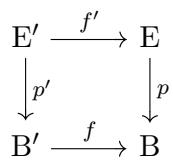
\includegraphics[keepaspectratio]{images/part001_3dd3ce93.jpg}}

a Cartesian square. If (E,p) is a locally trivial B-fibered space (resp. a covering), then (E',p') is a locally trivial fibered space (resp. a covering) with base B', trivializable if (E,p) is.

This follows from Corollary 1, applied with B = A and E' = B'.

COROLLARY 3. --- Let B be a topological space. Let E and E' be locally trivial B-fibered spaces (resp. coverings). Then \(E \times_{B} E'\) is a locally trivial B-fibered space (resp. a covering of B). It is trivializable if E and E' are.

This follows from Corollary 1, applied to the case where A, B, and B' are equal.

PROPOSITION 3. --- Let

\begin{enumerate}
\def\labelenumi{(\arabic{enumi})}
\tightlist
\item
\end{enumerate}

\pandocbounded{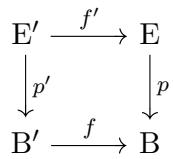
\includegraphics[keepaspectratio]{images/part001_0991252f.jpg}}

a Cartesian square. Suppose that in a neighborhood of every point of B, the map f has a continuous section. Then, if (E', p') is a locally trivial B'-fibered space (resp. a covering), the B-space (E, p) is a locally trivial fibered space (resp. a covering).

We need to prove that every point \(a\) of B has a neighborhood U such that the U-space induced by \((\mathrm{E}, p)\) over U is a locally trivial fibered space (resp. a covering). Take U to be a neighborhood of \(a\) over which there exists a continuous section \(s\) of \(f\). Denote by \(i: \mathrm{U} \to \mathrm{B}\) and \(j: \overline{p}^{-1}(\mathrm{U}) \to \mathrm{E}\) the canonical injections. Since square (1) is Cartesian, there exists a unique continuous map \(s^{\prime}\colon \overline{p}^{1}(\mathrm{U})\to \mathrm{E}^{\prime}\) such that \(f^{\prime}\circ s^{\prime} = j\) and \(p^{\prime}\circ s^{\prime} = s\circ p_{\mathrm{U}}\). The square

\[
\begin{array}{c} \stackrel {{- 1}} {{p}} (\mathrm{U}) \xrightarrow {s ^ {\prime}} \mathrm{E} ^ {\prime} \\ \Biggl \downarrow p _ {\mathrm{U}} \\ \mathrm{U} \xrightarrow {s} \mathrm{B} ^ {\prime} \end{array}\tag{2}
\]

is thus commutative, and its composite with square (1) is the Cartesian square.

\[
\begin{array}{c} \overline {{p}} ^ {1} (\mathrm{U}) \xrightarrow {j} \mathrm{E} \\ \Biggl \downarrow p _ {\mathrm{U}} \\ \mathrm{U} \xrightarrow {i} \mathrm{B}. \end{array}
\]

By proposition 7 of I, p. 15, the square (2) is Cartesian. Corollary 2 allows us to conclude.

Note. --- If in Proposition 3 one weakens the hypothesis on the map f by assuming only that it is universally strict and surjective, and if \(p'\) is a covering, the map p is étale (I, p. 31, prop. 8) and separated (I, p. 27, prop. 4), but E is not necessarily a covering of B. For example, one can find a topological space B and a locally finite closed covering \((\mathrm{A}_{i})_{i\in\mathrm{I}}\) of B, a B-space \((\mathrm{E},p)\) which is not a covering but such that, for every \(i\in I\), the \(A_{i}\)-induced space \(E_{A_{i}}\) is a covering of \(A_{i}\) (I, p. 146, exerc. 5). For a sufficient condition, see, however, Corollary 4 of I, p. 77.

\subsection{Degree of a covering}

Let B be a topological space, let E be a covering of B, and denote its projection by p. Let C be the set of cardinals \(\operatorname{Card}(\overline{p}^{1}(b))\), where b ranges over B. The map \(b \mapsto \operatorname{Card}(\overline{p}^{1}(b))\) is a locally constant map from B to C. One says that the covering E has a degree if B is nonempty and if the map \(b \mapsto \operatorname{Card}(\overline{p}^{1}(b))\) is constant. The common value of the cardinals \(\operatorname{Card}(\overline{p}^{1}(b))\), for \(b \in B\), is then called the degree of the covering E and is denoted \(\deg(E, p)\), or simply \([E:B]\) if there can be no ambiguity about the map p.

If B is not empty, the trivial covering with base B and fiber type F has a degree equal to Card(F).

If B is connected, the function \(b \mapsto \text{Card}(\overline{p}^{1}(b))\) is constant. Consequently:

PROPOSITION 4. --- Every covering of a nonempty connected space has a degree.

Let G be a topological space, let \((\mathrm{F}, g)\) be a covering of G and let \((\mathrm{E}, f)\) be a covering of F; suppose that these coverings have a degree. If the G-space \((\mathrm{E}, g \circ f)\) is a covering, then it has a degree and one has \(\deg(\mathrm{E}, g \circ f) = \deg(\mathrm{F}, g) \deg(\mathrm{E}, f)\), which can also be written

\[
[ \mathrm{E}: \mathrm{G} ] = [ \mathrm{E}: \mathrm{F} ] [ \mathrm{F}: \mathrm{G} ].
\]

Indeed, if z is a point of G, all the fibers of the map

\[
f _ {g (z)} ^ {- 1}: \stackrel {{- 1}} {{f}} (\stackrel {{- 1}} {{g}} (z)) \to \stackrel {{- 1}} {{g}} (z)
\]

have cardinality \(\deg(\mathrm{E}, f)\), and \(\overline{g}^1(z)\) has cardinality \(\deg(\mathrm{F}, g)\). The assertion therefore follows from the shepherd's principle (E, III, p. 41, prop. 9).

Let B and B' be topological spaces, let (E, p) be a covering of B and let (E', p') be a covering of B'. Suppose that these coverings have a degree; then the covering (E × E', p × p') of B × B' (I, p. 71, prop. 2) has a degree and one has:

\[
\deg (\mathrm{E} \times \mathrm{E} ^ {\prime}, p \times p ^ {\prime}) = \deg (\mathrm{E}, p) \deg (\mathrm{E} ^ {\prime}, p ^ {\prime}).
\]

Indeed, for every pair \((b,b^{\prime})\in\mathrm{B}\times\mathrm{B}^{\prime}\), the fiber \((\mathrm{E}\times\mathrm{E}^{\prime})_{(b,b^{\prime})}\) is the product \(E_{b}\times E_{b^{\prime}}^{\prime}\) .

Let B and B' be topological spaces, let (E, p) be a covering of B, let (E', p') be a covering of B', and let

\[
\begin{array}{c} \mathrm{E} ^ {\prime} \xrightarrow {f ^ {\prime}} \mathrm{E} \\ \Biggl \downarrow p ^ {\prime} \\ \mathrm{B} ^ {\prime} \xrightarrow {f} \mathrm{B} \end{array}
\]

a Cartesian square. If B′ is nonempty and if the covering (E, p) has a degree, then the covering (E′, p′) has a degree, equal to that of E, by I, p. 10, cor. of prop. 4.

\subsection{Finite coverings}

A covering is said to be locally finite if the cardinalities of all its fibers are finite. A covering is said to be finite if the set of cardinalities of its fibers is bounded above by a finite cardinal.

THEOREM 1. --- Let E, B be topological spaces and \(p\colon\mathrm{E}\to\mathrm{B}\) a map. The following conditions are equivalent:

\begin{enumerate}
\def\labelenumi{(\roman{enumi})}
\item
  The space E, equipped with the map p, is a locally finite covering of B;
\item
  The map p is étale, proper, and separated;
\item
  The map p is continuous, open, and separated, its fibers are finite, and the numerical function \(b \mapsto \text{Card}(\overline{p}^{1}(b))\) is upper semicontinuous on B (TG, IV, p. 28).
\end{enumerate}

We will use the following lemma in the proof:

Lemma. — Let X and Y be topological spaces. For a map \(f: X \to Y\) to be closed, it is necessary and sufficient that for every point y of Y and every neighborhood W of the fiber \(f^{-1}(y)\) there exists a neighborhood V of y such that W contains \(f^{-1}(V)\) .

In this statement, one may consider only the neighborhoods W of \(f^{-1}(y)\) which are open. Denoting by F the complement of W in X, one can then reformulate the statement as follows: for a map \(f: X \to Y\) to be closed, it is necessary and sufficient that, for every closed subset F of X, every point y of Y that does not belong to \(f(F)\) has a neighborhood V disjoint from \(f(F)\). Now this assertion follows immediately from the definition of a closed map (TG, I, p. 30, def. 1).

Let us now prove Theorem 1. Each of the three conditions implies that the map p is continuous, open, and separated, and also that the fibers of p are finite. This is clear under hypotheses (i) and (iii); under hypothesis (ii), the fibers of p are discrete (I, p. 29, remark 2) and quasi-compact (TG, I, p. 75, th. 1), hence finite (TG, I, p. 60, example 1).

(i)⇒(ii): it suffices to show that p is proper and, for this, that for every open set U over which the covering (E,p) is trivializable, the map \(p_{\mathrm{U}}\colon \overline{p}^{1}(\mathrm{U})\to\mathrm{U}\) is proper (TG, I, p. 72, prop. 3).

As the fibers of \(p_{U}\) are finite, this last assertion follows from Corollary 5 of TG, I, p. 77.

(ii)⇒(iii): let b be a point of B and, for every \(x \in \overline{p}^{1}(b)\), let \(W_{x}\) be an open neighborhood of x in E such that \(p \mid W_{x}\) is injective. The set \(W = \bigcup_{x \in \overline{p}^{1}(b)} W_{x}\) is an open neighborhood of \(\overline{p}^{1}(b)\). Since the map p is closed, it follows from the lemma above that there exists an open neighborhood U of b such that \(\overline{p}^{1}(U) \subset W\). For all \(a \in U\), we have \(\overline{p}^{1}(a) \subset W\); since the restriction of p to each \(W_{x}\) is injective, it follows that \(\text{Card}(\overline{p}^{1}(a)) \leqslant \text{Card}(\overline{p}^{1}(b))\), which proves the upper semicontinuity of the map \(a \mapsto \text{Card}(\overline{p}^{1}(a))\).

(iii)⇒(i): let b be a point of B. Since the fiber \(E_{b} = \overline{p}^{1}(b)\) is finite and the map p is separated, one can choose, for every \(x \in E_{b}\), an open neighborhood \(V_{x}^{\prime}\) of x such that the \(V_{x}^{\prime}\) are pairwise disjoint (I, p. 26, Remark 4). Since the map p is open and the set \(E_{b}\) finite, the set \(U^{\prime} = \bigcap_{x \in E_{b}} p(V_{x}^{\prime})\) is an open neighborhood of b in B. Let U be an open neighborhood of b in B, contained in \(U^{\prime}\) and such that for all \(a \in U\), \(\text{Card}(E_{a}) \leqslant \text{Card}(E_{b})\). For all \(x \in E_{b}\), set \(V_{x} = V_{x}^{\prime} \cap \overline{p}^{1}(U)\). Let a be a point of U; the sets \(E_{a} \cap V_{x}\), for \(x \in E_{b}\), are nonempty and pairwise disjoint. These sets therefore each contain a unique element and form a partition of \(E_{a}\). This proves that, for every \(x \in E_{b}\), the map \(p | V_{x}\) is injective and that we have \(\overline{p}^{1}(U) = \bigcup_{x \in E_{b}} V_{x}\). Since the map p is open, it induces a homeomorphism from \(V_{x}\) onto U, and consequently, (E, p) is a covering of B (I, p. 70, cor. 1 of prop. 1).

Remark. --- A continuous, separated, open, proper map with finite fibers is not necessarily a covering. This is the case for the map \(x \mapsto x^{2}\) from R to \([0; +\infty[\) .

COROLLARY 1. --- Let E and B be topological spaces and let \(p\colon\mathrm{E}\to\mathrm{B}\) a proper and separated map. The set U of points b in B such that p is étale at every point of the fiber \(\mathrm{E}_{b}\) is open in B. The U-space induced by (E,p) over U is a locally finite covering.

The set F of points of E at which the map p is not étale is closed in E (I, p. 29, remark 1). Its image \(p(\mathrm{F})\) is closed because the map p is proper; the complement U of \(p(\mathrm{F})\) is therefore open. The map \(p_{U}\) is separated (I, p. 27, prop. 4) and proper (TG, I, p. 72, prop. 3). By construction, the map \(p_{\mathrm{U}}\) is étale; it therefore satisfies condition (ii) of Theorem 1.

COROLLARY 2. — Let B be a separated topological space and let E be a B-space. Suppose that E is compact and that its projection p: E → B is étale. Then E is a finite covering of B.

The map \(p\) is separated (I, p. 26, remark 2) and proper (TG, I, p. 76, cor. 2). By Corollary 1, E is therefore a locally finite covering of B. Since E is compact, \(p(\mathrm{E})\) is a quasi-compact subset of B; the map from \(p(\mathrm{E})\) into \(\mathbb{N}\) given by \(b \mapsto \operatorname{Card} \overline{p}^1(b)\) is locally constant, and is therefore bounded above (TG, IV, p. 30, corollary).

COROLLARY 3. --- Let B be a topological space, let (E,p) and (E',p') be B-spaces, and let f: E' → E be a B-morphism. Suppose that E' is a locally finite covering of B.

\begin{enumerate}
\def\labelenumi{\alph{enumi})}
\item
  If the map p is étale and separated, the E-space (E', f) is a covering.
\item
  If the map f is surjective and makes the space E' a covering of E, then E is a covering of B.
\end{enumerate}

Under the assumption \(a\), the maps \(p\) and \(p'\) are étale and separated, and the map \(p'\) is proper (Theorem 1). The map \(f\) is therefore étale (I, p. 30, cor. 1 of prop. 6), separated (I, p. 25, prop. 2 b)) and proper (I, p. 28, prop. 5). By Theorem 1, \((\mathrm{E}', f)\) is a covering of E.

Suppose now that \(f\) is surjective and suppose that \((\mathrm{E}', f)\) is a covering of E. It is then locally finite, so the map \(f\) is proper and surjective (th. 1). By I, p. 25, prop. 2, c), the map \(p\) is separated, since \(p' = p \circ f\) and \(p'\) is separated. The map \(p\) is étale (I, p. 29, prop. 6, d)), proper (TG, I, p. 73, prop. 5, b)), and its fibers are finite. By th. 1, the B-space \((\mathrm{E}, p)\) is then a covering of B.

COROLLARY 4. --- Let

\[
\begin{array}{c} \mathrm{E} ^ {\prime} \xrightarrow {f ^ {\prime}} \mathrm{E} \\ \Big \downarrow p ^ {\prime} \\ \mathrm{B} ^ {\prime} \xrightarrow {f} \mathrm{B} \end{array}
\]

a Cartesian square. Suppose that \((\mathrm{E}^{\prime}, p^{\prime})\) is a locally finite covering of \(B^{\prime}\) and that the map f is universally strict and surjective. Then \((\mathrm{E}, p)\) is a locally finite covering of B.

Indeed, the map p is étale (I, p. 31, prop. 8), proper (I, p. 21, prop. 11), and separated (I, p. 27, prop. 4).

COROLLARY 5. --- Let B be a connected topological space and let (E, p) be a finite covering of B. The space E has only finitely many connected components, and each of them is a covering of B.

The result is true if B is empty; we henceforth assume it to be nonempty. If X is a clopen subset of E, the restriction of p to X is a separated map (I, p. 25, prop. 2, a) and I, p. 26, remark 1), étale and proper (TG, I, p. 74, corollary 1); by Theorem 1, (X, p) is a locally finite covering of B. Since B is connected, this covering has finite degree. If X is distinct from E, there exists a point \(b \in B\) such that \(X_{b} \subsetneq E_{b}\), whence \([X:B] < [E:B]\). Since B is connected, it follows that every decreasing sequence of closed-open sets in E is stationary.

Let \(x \in E\); there then exists a smallest open and closed subset X of E containing x (E, III, p. 51, prop. 6). Such a set X is connected; it is therefore the connected component of x in E. This shows that the connected components of E are open and closed and that each of them is a covering of B. Since B is connected, each connected component of E meets every fiber of p; hence the connected components of E are finite in number.

PROPOSITION 5. — Let B be a topological space, let E and E′ be B-spaces, and let f: E′ → E be a B-morphism. Suppose that E is a locally finite covering and that the space E′, equipped with the map f, is a locally trivial E-fibered space (resp. a covering). Then E′ is a locally trivial B-fibered space (resp. a covering).

Denote by \(p\) and \(p'\) the respective projections of the B-spaces E and E'. Let \(b\) be a point of B. There exists an open neighborhood U of \(b\) in B and a finite partition \((\mathrm{V}_i)_{i\in \mathrm{I}}\) of \(\overline{p}^1 (\mathrm{U})\) formed by open sets of E such that, for every \(i\in \mathrm{I}\), the map \(p\) induces a homeomorphism of \(\mathrm{V}_i\) onto U. Set \(\mathrm{V}_i' = f^{-1}(\mathrm{V}_i)\). The sets \(\mathrm{V}_i'\) are open in E', form a partition of \(\overline{p'}^{1}(\mathrm{U})\), and the map from \(\mathrm{V}_i'\) to U induced by \(p'\) by passing to subspaces makes \(V_i'\) a locally trivial U-fibered space. It follows that the space \(\overline{p'}^{1}(\mathrm{U})\), equipped with the map \(p_U': \overline{p'}^{1}(\mathrm{U}) \to U\), is a locally trivial U-fibered space (I, p. 69, remark 2). If \((E', f)\) is a covering of E, the fibers of \(p_U'\) are discrete because their intersections with each of the open sets \(V_i'\) are discrete. This completes the proof.

Note. --- If (E, p) is a covering of B and (E', f) is a covering of E, the map \(p \circ f\) is étale (I, p. 29, prop. 6, a)) and separated (I, p. 25, prop. 2, a)). But it can happen, see Exercise 5, b) of I, p. 146, that the space E′, equipped with the map \(p \circ f\), is not a covering of B. See, however, IV, p. 342, prop. 3.

\subsection{Coverings of locally connected spaces}

Let B be a topological space and let E be a B-space. Suppose that its projection p is an étale and separated map.

If the space B is locally connected, the space E is locally connected. If the space E is locally connected, the open subset \(p(\mathrm{E})\) of B (cf. I, p. 29, remark 2) is locally connected.

The image \(s(\mathrm{B})\) of any section \(s\) of \(p\) is open (I, p. 30, cor. 3) and closed in B (I, p. 27, prop. 3). If B is connected and nonempty, it is therefore a connected component of E; in general, it is a union of connected components of E.

If B is locally connected, the union of the images of the sections of p is therefore an open and closed subset of E (cf. TG, I, p. 85).

Suppose that E is a trivializable covering of B, and let \(g: E \to B \times F\) be a trivialization. If the space B is connected, the sets \(V_{x} = \overline{g}^{1}(B \times \{x\})\) as x runs through F, are the connected components of E (cf. prop. 1 of I, p. 69).

PROPOSITION 6. --- Let B be a topological space and let E be a B-space; denote its projection by p. Suppose that the space E is locally connected. For E to be a covering of B, it is necessary and sufficient that every point of B have an open neighborhood U such that the map p induces a homeomorphism from every connected component of \(\overline{p}^{1}(U)\) onto U.

Let \(b\) be a point of B. If E is a covering of B, every open neighborhood U of \(b\) which is connected and over which the covering E is trivializable satisfies the conditions stated in the proposition. Conversely, let U be an open neighborhood of \(b\) satisfying these conditions. The set \(\overline{p}^{1}(\mathrm{U})\) is open; its connected components are open subsets of E (TG, I, p. 85, prop. 11) and form a partition of \(\overline{p}^{1}(\mathrm{U})\). The proposition therefore follows from Corollary 1 (I, p. 70) of Proposition 1.

COROLLARY 1. — Let B be a locally connected topological space, let (E,p) be a covering of B, and let E' be an open and closed subset of E. The B-space (E',p \textbar{} E') is a covering, and p(E') is both open and closed in B.

The spaces E and E′ are locally connected. For every open subset U of B, the set \(\mathrm{E}'\cap\overline{p}^{1}(\mathrm{U})\) is open and closed in \(\overline{p}^{1}(\mathrm{U})\), therefore it is a union of connected components of \(\overline{p}^{1}(\mathrm{U})\). The open subsets U of B such that p induces a homeomorphism from each connected component of \(\overline{p}^{1}(\mathrm{U})\) onto U cover B. By the proposition, \(p\mid E'\) makes \(E'\) a covering of B. The second assertion follows from this (cf. I, p. 68).

COROLLARY 2. --- Let B be a locally connected topological space, let (E,p), (E',p') be coverings of B, and let f,g: E' → E be B-morphisms. For every point b of B, denote \(f_b,g_b\) : \(\mathrm{E}_b\to \mathrm{E}_b'\) the maps induced by f and g, respectively. The set of points b in B such that \(f_b = g_b\) is open and closed in B.

Let X be the set of points x in \(E'\) such that \(f(x) = g(x)\). This is the set of points where the lifts f and g of \(p'\) to E coincide; hence X is open and closed in \(E'\) (prop. 11 of I, p. 34). The complement Y of X is also open and closed; consequently \(p(Y)\) is open and closed in B (corollary 1). Its complement, which is the set of points b of B such that \(f_{b} = g_{b}\) , is therefore also open and closed.

COROLLARY 3. --- Let B be a connected and locally connected topological space, and let (E, p) and (E', p') be coverings of B. For every point b of B, the map \(f \mapsto f_b\) from \(\mathcal{C}_{\mathrm{B}}(\mathrm{E}'; \mathrm{E})\) to \(\mathcal{C}(\mathrm{E}_b'; \mathrm{E}_b)\) is injective.

Let \(b\) be a point of B. Let \(f\) and \(g\) be B-morphisms from E' to E such that \(f_b = g_b\). The set of points \(a\) of B such that \(f_a = g_a\) is open and closed in B (corollary 2) and contains b. It is therefore equal to B, and f is equal to g.

COROLLARY 4. --- Let B be a connected and locally connected topological space, let (E, p) be a covering of B, and let b be a point of B. For E to be a trivializable covering, it is necessary and sufficient that every point of the fiber \(E_{b}\) belong to the image of a continuous section of p.

The condition is necessary. Let \(E'\) be the union of the images of the continuous sections of p, and let \(E''\) be its complement in E. The set \(E'\) is open and closed in E (cf. I, p. 79). Consequently, \((\mathrm{E}', p \mid \mathrm{E}')\) is a covering of B (Corollary 1), and this covering is trivializable by virtue of Corollary 2 (I, p. 70). Suppose that \(E'\) contains \(E_b\) and let us prove that \(E''\) is empty. Since \(E''\) is open and closed in E, \(p(\mathrm{E}'')\) is open and closed in B (corollary 1). Since B is connected and b does not belong to \(p(\mathrm{E}'')\), \(p(\mathrm{E}'') = \varnothing\), therefore \(E'' = \varnothing\).

COROLLARY 5. --- Let

\pandocbounded{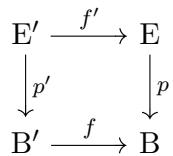
\includegraphics[keepaspectratio]{images/part001_2db9b8ac.jpg}}

a Cartesian square. Suppose that the B-space (E, p) is a covering and that the space B' is connected and locally connected. Let b' be a point of B'. For the B'-space (E', p') to be a trivializable covering, it is necessary and sufficient that for every point x of E such that \(p(x) = f(b')\) there exists a continuous lifting \(g: B' \to E\) of f such that \(g(b') = x\).

Recall that \((\mathrm{E}^{\prime}, p^{\prime})\) is a covering of \(B^{\prime}\) (I, p. 71, cor. 2) and that the map \(f^{\prime}\) induces a bijection \(E_{b^{\prime}}^{\prime} \to E_{f(b^{\prime})}\) (I, p. 10, cor.). By prop. 3 of I, p. 9, the map \(s \mapsto f^{\prime} \circ s\) defines a bijection between the set of continuous sections of \(p^{\prime}\) and the set of continuous lifts of f to E. The corollary therefore follows from Corollary 4.

PROPOSITION 7. --- Let B be a topological space, let E and E' be B-spaces, and let f: E' → E be a B-morphism. Suppose that E' is a covering of B and that the space B is locally connected.

\begin{enumerate}
\def\labelenumi{\alph{enumi})}
\item
  If the projection of the B-space E is an étale and separated map, \((\mathrm{E}^{\prime}, f)\) is a covering of E.
\item
  If f is surjective, then E is a covering of B.
\end{enumerate}

Denote by \(p\) and \(p'\) the projections of the B-spaces E and E′ respectively. Under hypothesis \(a\), \(f\) is étale (I, p. 29, prop. 6, c)). Under hypothesis \(b\), \(p\) is étale (loc. cit., d)). Consequently, under either of these two hypotheses, E is locally connected; its connected components are in particular open and closed in E (TG, I, p. 85, prop. 11).

We shall first prove Proposition 7 under the additional assumption that B is connected, locally connected, and that E' is the trivial covering (B × F', pr₁).

Lemma. --- If U is a connected component of E', the restriction of f to U induces a homeomorphism from U onto a connected component of E.

Let \(x \in F'\) such that \(U = B \times \{x\}\) (cf. I, p. 79). The map from B to E that sends \(b \in B\) to \(f(b, x)\) is a continuous section of p. Its image X is therefore connected and open in E, since p is étale (I, p. 30, cor. 3). It is moreover closed under hypothesis a), since p is separated (I, p. 27, prop. 3). It is also closed under hypothesis b) by Corollary 1 of I, p. 80, since U is open and closed in E'. Consequently, X is a connected component of E.

Since \(f \mid \mathrm{U} \colon \mathrm{U} \to \mathrm{X}\) is bijective and open, it is a homeomorphism onto its image, which proves the lemma.

Let us keep the hypotheses preceding the lemma and now prove assertion \(a\) ). Let V be a connected component of E. It is an open and closed set in E, and \(f^{-1}(\mathrm{V})\) is a union of connected components of \(\mathrm{E}'\) which \(f\) maps homeomorphically onto V by the lemma. It follows from prop. 6 of I, p. 79 that \((\mathrm{E}', f)\) is a covering.

Let us prove b). Since f is surjective, it follows from the lemma that every connected component V of E is the homeomorphic image of a connected component \(U = B \times \{x\}\) of \(E'\) . The map p then induces a homeomorphism from V onto B. By prop. 6, E is a covering of B.

This therefore proves the proposition, under the additional hypothesis that B is connected and E' is a trivializable covering of B. Let us prove it in the general case.

There exists a covering \((\mathrm{U}_{i})_{i\in\mathrm{I}}\) of B, consisting of connected open sets over which the covering \(E'\) is trivializable. Let \(i\in I\) .

Let us prove \(a\). If the map \(p\) is étale and separated, the same is true of the map \(p_{\mathrm{U}_i}\colon \mathrm{U}_i\times_{\mathrm{B}}\mathrm{E}\to \mathrm{U}_i\), for \(i\in \mathrm{I}\), by props. 8 of I, p. 31 and 4 of I, p. 27. It follows therefore from the particular case treated that, for every \(i\in \mathrm{I}\), the \(\mathrm{U}_i\)-space \((\overline{p'}^{1}(\mathrm{U}_i),f_{\mathrm{U}_i})\) is a covering. Let A denote the total space of the disjoint union \(\coprod_{i\in I}\mathrm{U}_i\) and \(q\colon \mathrm{A}\to \mathrm{B}\) the canonical map. Then, the space \(\mathrm{A}\times_{\mathrm{B}}\mathrm{E}'\), equipped with the map \(f_{\mathrm{A}}\colon \mathrm{A}\times_{\mathrm{B}}\mathrm{E}'\to \mathrm{A}\times_{\mathrm{B}}\mathrm{E}\), is a covering of \(\mathrm{A}\times_{\mathrm{B}}\mathrm{E}\). The map \(q\) admits a continuous section in a neighborhood of every point of B, and Proposition 3 of I, p. 72, applied to the Cartesian square

\[
\begin{array}{c} \mathrm {A\times_ {B} E^ {\prime}} \longrightarrow \mathrm {E^ {\prime}} \\ \Big \downarrow f _ {\mathrm{A}} \\ \mathrm {A\times_ {B} E} \longrightarrow \mathrm{E} \end{array} ,
\]

implies that \(E'\) is a covering of E.

Let us prove \(b\). Suppose that \(f\) is surjective. Then, for every element \(i\) from I, the map \(f_{\mathrm{U}_i}\colon \mathrm{U}_i\times_{\mathrm{B}}\mathrm{E}'\to \mathrm{U}_i\times_{\mathrm{B}}\mathrm{E}\) is surjective and the space \(\mathrm{U}_i\times_{\mathrm{B}}\mathrm{E}'\), equipped with the map \(f_{\mathrm{U}_i}\), is a covering of \(\mathrm{U}_i\times_{\mathrm{B}}\mathrm{E}\) (I, p. 71, cor. 2 of prop. 2). From the special case treated previously, it follows that the \(\mathrm{U}_i\)-space \((\overline{p}^{1}(\mathrm{U}_{i}),p_{\mathrm{U}_{i}})\) is a covering. Consequently, E is a covering of B.

Let B be a topological space, let E and E′ be coverings of B, and let \(f: E \rightarrow E'\) be a B-morphism. We have seen that \((E, f)\) is a covering under each of the following two hypotheses: 1) the covering E is locally of finite degree (I, p. 76, cor. 1); 2) the space B is locally connected (I, p. 81, prop. 7). This phenomenon can be explained as follows.

Let F and F′ be discrete topological spaces, and let \(f: B \times F \to B \times F'\) be a B-morphism. The map \(\widetilde{f}: b \mapsto \mathrm{pr}_{2} \circ f(b, \cdot)\) from B to the space \(\mathcal{C}_{c}(F; F')\) is continuous (TG, X, p. 28, th. 3). If U is an open subset of B such that the map \(\widetilde{f}\) is constant on U, the map \(f_{U}: U \times F \to U \times F'\) deduced from f is a trivializable covering (I, p. 69, prop. 1).

The space \(\mathcal{C}_c(\mathrm{F};\mathrm{F}')\) is none other than the set \(\mathcal{F}(\mathrm{F};\mathrm{F}')\) of maps from F into \(\mathrm{F}'\) endowed with the topology induced by the topology of the product space \((\mathrm{F}')^{\mathrm{F}}\) by the canonical identification. For this topology, the space \(\mathcal{F}(\mathrm{F};\mathrm{F}')\) is totally disconnected (I, p. 84, prop. 10). Consequently, if the space B is connected, the map \(\widetilde{f}\) is constant (I, p. 82, prop. 4); if the space B is locally connected, the map \(\widetilde{f}\) is locally constant. When the set F is finite, the space \(\mathcal{F}(\mathrm{F};\mathrm{F}')\) is discrete and the map \(\widetilde{f}\) is locally constant.

Remark. --- Let B be a topological space, let \((\mathrm{E}, p)\) and \((\mathrm{E}', p')\) be B-spaces and let \(f: E' \to E\) be a B-morphism.

\begin{enumerate}
\def\labelenumi{\alph{enumi})}
\item
  If E and E' are coverings of B, the map f is étale (I, p. 29, prop. 6) and separated (I, p. 25, prop. 2). But it is not true in general that (E', f) is a covering of E if the space B is not locally connected (I, p. 145, exerc. 4).
\item
  If \((\mathrm{E}^{\prime}, p^{\prime})\) is a covering of B, f is surjective and makes \(E^{\prime}\) a covering of E, then the map p is étale (I, p. 29, prop. 6). But it is not true, in general, that it is separated if the space B is not locally connected (I, p. 145, exerc. 4). In particular, E is not necessarily a covering of B.
\end{enumerate}

COROLLARY. --- Let B be a connected and locally connected topological space. Let E and E' be coverings of B. Let b be a point of B. Let \(f: E' \to E\) be a B-morphism and let \(f_{b}: E_{b}' \to E_{b}\) be the map induced by f by restriction to the fibers. If the map \(f_{b}\) is injective (resp. surjective, resp. bijective), then so is the map f.

Denote by \(p\) the projection of the B-space E. According to the proposition, \((\mathrm{E}', f)\) is a covering of E; its image \(f(\mathrm{E}')\) is open and closed in E. Let U denote the complement of \(f(\mathrm{E}')\) in E, so that the B-space \((\mathrm{U}, p \mid \mathrm{U})\) is a covering of B (I, p. 80, corollary 1). If the map \(f_b\) is surjective, the fiber at \(b\) of this covering is empty. Since B is a connected space, U is then empty, so \(f\) is surjective.

The set V of points of E where the fiber of f has exactly one element is open and closed. The B-spaces \((V, p|V)\) and \((f(E'), p|f(E'))\) are coverings of B (loc. cit.) and the canonical map \(i: V \to f(E')\) is a B-morphism. If the map \(f_b\) is injective, the map \(i_b\) is surjective, hence i is surjective by the preceding result, and we have \(V = f(E')\). Consequently, the map f is injective.

\subsection{Coverings of a paracompact space}

PROPOSITION 8. --- A covering of a paracompact space (I, p. 69) is a paracompact space.

Let us first prove a lemma.

Lemma. --- Let E be a separated topological space. Suppose that E has a locally finite open cover \((\mathrm{V}_{i})_{i\in\mathrm{I}}\) such that, for every \(i\in I\), \(\overline{V_{i}}\) is a paracompact space. Then the space E is paracompact.

Let \((\mathrm{W}_{j})_{j\in\mathrm{J}}\) be an open cover of E; we shall prove that there exists a locally finite open refinement \((\mathrm{A}_{k})_{k\in\mathrm{K}}\) of E which is finer than the covering \((\mathrm{W}_{j})_{j\in\mathrm{J}}\). For all \(i\in I\), let \((\mathrm{A}_{\ell}^{\prime})_{\ell\in\mathrm{K}_{i}}\) be a locally finite covering of \(\overline{V_{i}}\) by open subsets of \(\overline{V_{i}}\), finer than the covering \((\mathrm{W}_{j}\cap\overline{\mathrm{V}_{i}})_{j\in\mathrm{J}}\). Let K be the sum of the family \((\mathrm{K}_{i})_{i\in\mathrm{I}}\) (E, II, p. 30, def. 8). For every element \(k=(\ell,i)\) of K, set \(A_{k}=A_{\ell}^{\prime}\cap V_{i}\). Then \(A_{k}\) is open in E and one has \(\bigcup_{k\in K}A_{k}=\bigcup_{i\in I}V_{i}=E\); moreover, for every \(k\in K\), there exists an index \(j\in J\) such that \(A_{k}\subset W_{j}\). Thus, the family \((\mathrm{A}_{k})_{k\in\mathrm{K}}\) is an open cover of E finer than \((\mathrm{W}_{j})_{j\in\mathrm{J}}\). It remains to prove that the family \((\mathrm{A}_{k})_{k\in\mathrm{K}}\) is locally finite. Let \(x\in E\); there exists an open neighborhood U of x that meets \(V_{i}\) only for i belonging to a finite subset I' of I. For every \(i\in I'\), x has an open neighborhood \(U_{i}\subset U\) that meets only finitely many open sets \(A_{k}\), for \(k\in K_{i}\times\{i\}\): this is obvious if x does not belong to \(\overline{V_{i}}\), and if x belongs to \(\overline{V_{i}}\), this follows from the local finiteness property of the covering \((\mathrm{A}_{\ell}^{\prime})_{\ell\in\mathrm{K}_{i}}\) of \(\overline{V_{i}}\). Consequently, \(V^{\prime}=\bigcap_{i\in I'}U_{i}\) is an open neighborhood of x that meets only finitely many of the \(A_{k}\), \(k\in K\), and the covering \((\mathrm{A}_{k})_{k\in\mathrm{K}}\) is locally finite.

Let us prove the proposition. Let E be a covering of B, denote its projection by p, and suppose that the space B is paracompact. Let \((\mathrm{A}_{i})_{i\in\mathrm{I}}\) be a locally finite open cover of B such that, for every \(i\in I\), the covering E is trivializable over \(A_{i}\). For all \(i\in I\), let \(F_{i}\) be a discrete topological space and let \(g_{i}\colon\overline{p}^{1}(\mathrm{A}_{i})\to\mathrm{A}_{i}\times\mathrm{F}_{i}\) be a trivialization of E over \(A_{i}\). Let \((\mathrm{B}_{i})_{i\in\mathrm{I}}\) be an open cover of B such that, for every \(i\in I\), one has \(\overline{B_{i}}\subset A_{i}\) (TG, IX, p. 49, prop. 4 and p. 48, cor. 1). For every \(i\in I\), set \(V_{i}=\overline{p}^{1}(\mathrm{B}_{i})\); we have \(\overline{V_{i}}\subset\overline{p}^{1}(\overline{\mathrm{B}_{i}})\subset\overline{p}^{1}(\mathrm{A}_{i})\) and \(V_{i}=\overline{g_{i}}^{1}(\mathrm{B}_{i}\times\mathrm{F}_{i})\), whence \(\overline{V_{i}}\subset\overline{g_{i}}^{1}(\overline{\mathrm{B}_{i}}\times\mathrm{F}_{i})\). Since B is paracompact, \(\overline{B_{i}}\) is paracompact (TG, I, p. 69, prop. 16) and \(\overline{B_{i}}\times F_{i}\) is paracompact (TG, I, p. 70, prop. 18). Consequently, \(\overline{g_{i}}^{1}(\overline{\mathrm{B}_{i}}\times\mathrm{F}_{i})\) is paracompact, hence \(\overline{V_{i}}\) also (TG, I, p. 69, prop. 16). The family \((\mathrm{V}_{i})_{i\in\mathrm{I}}\) is, by construction, a locally finite open covering of E. Finally, the space E is separated (I, p. 26, remark 3). It therefore satisfies the hypotheses of the lemma, whence the proposition.

Remark. --- One can show that a covering of a metrizable space is metrizable (I, p. 145, exerc. 1) and that a connected covering of a locally compact, countable-at-infinity space is itself locally compact and countable at infinity (I, p. 145, exerc. 2).

\subsection{Locally constant sheaves}

Let B be a topological space and F a set; endow F with the discrete topology. One calls the constant sheaf on B with stalk-type F the sheaf on B of locally constant functions with values in F (I, p. 45, example 2). This sheaf is sometimes denoted \(\underline{\mathbf{F}}\), when no confusion about the space B is to be feared. It is identified with the sheaf on B of continuous sections of the étale B-space \((B \times F,\mathrm{pr}_1)\): the formula \(i([U,s,a]) = (a,s(a))\) indeed defines a canonical isomorphism \(i\) from the étalé space associated with \(\underline{\mathbf{F}}\) onto \((B \times F,\mathrm{pr}_1)\). For every \(a \in B\), the map \([U,s,a] \mapsto s(a)\) is a canonical bijection of the stalk \(\underline{\mathbf{F}}_a\) of \(\underline{\mathbf{F}}\) at \(a\) onto the set F.

Let \(\mathcal{P} = (\mathcal{P}(\mathrm{U}), r_{\mathrm{UV}})\) be the presheaf on B such that \(\mathcal{P}(\mathrm{U}) = \mathrm{F}\) for every open set U of B and \(r_{\mathrm{UV}} = \mathrm{Id}_{\mathrm{F}}\) for every pair (U, V) of open sets of B such that \(\mathrm{U} \subset \mathrm{V}\). Then, the sheaf \(\widetilde{\mathcal{P}}\) associated with \(\mathcal{P}\) is canonically isomorphic to the constant sheaf \(\underline{\mathrm{F}}\) (I, p. 52, example 1).

DEFINITION 3. --- A sheaf \(\mathcal{F}\) on a topological space B is locally constant if every point of B has an open neighborhood U such that the induced sheaf \(\mathcal{F} \mid U\) is isomorphic to a constant sheaf on U.

PROPOSITION 9. --- For a sheaf to be locally constant, it is necessary and sufficient that the associated étalé space be a covering.

Let B be a topological space and let \(\mathcal{F}\) be a sheaf on B. The sheaf \(\mathcal{F}\) is constant if and only if the étalé space \(\mathrm{E}_{\mathcal{F}}\) is B-isomorphic to a trivial covering \((\mathrm{B} \times \mathrm{F},\mathrm{pr}_1)\), where F is a discrete topological space. If U is an open subset of B, the étalé space associated with the induced sheaf \(\mathcal{F} \mid \mathrm{U}\) is identified with the U-étale space induced by \(\mathrm{E}_{\mathcal{F}}\) above U (cf. I, p. 51). The proposition follows from this.

COROLLARY. --- For an étale B-space to be a covering, it is necessary and sufficient that the sheaf of its sections be locally constant.

This follows from the proposition and from Example 2 of I, p. 52.

\subsection{Products of locally constant sheaves}

Let B be a topological space and let \((\mathcal{F}_{i})_{i\in\mathrm{I}}\) be a family of sheaves on B. Denote by \(\mathcal{F}\) the product sheaf \(\prod_{i\in I}\mathcal{F}_{i}\) and, for \(i\in I\), let \(pr_{i}\colon \mathcal{F}\to\mathcal{F}_{i}\) be the projection morphism of index i (I, p. 46, example 7). Let \((\mathrm{E},p)\) and \((\mathrm{E}_{i},p_{i})\) be the étalé B-spaces associated with the sheaves \(\mathcal{F}\) and \(\mathcal{F}_{i}\), respectively, and let \(\varphi_{i}\colon \mathrm{E}\to \mathrm{E}_{i}\) be the B-morphism associated with \(pr_{i}\) (I, p. 50). Finally, let us denote by \((\mathrm{E}^{\prime},p^{\prime})\) the B-product \(\prod_{B}\mathrm{E}_{i}\). By the universal property of the B-space product (I, p. 5), there exists a unique B-morphism \(\Phi\colon \mathrm{E}\to \mathrm{E}^{\prime}\) such that, for every \(i\in I\), \(pr_{i}\circ\Phi=\varphi_{i}\).

PROPOSITION 10. --- If the set I is finite, the B-morphism \(\Phi\) is an isomorphism.

By the corollary of I, p. 32, the B-space \(\mathrm{E}'\) is étale, and it suffices to show that the B-morphism \(\Phi\) is bijective (I, p. 30, cor. 2). For every point b of B, the restriction \(\Phi_b\colon \mathrm{E}_b\to \mathrm{E}'_b\) of \(\Phi\) to the fibers at b is identified with the canonical map from \(\varinjlim\prod_{i\in I}\mathcal{F}_{i}(U)\) to \(\prod_{i\in I}\varinjlim\mathcal{F}_{i}(U)\), where U ranges over the open subsets of B containing b (cf. I, p. 50). By prop. 10 of E, III, p. 67, this map is a bijection.

Now consider the case of locally constant sheaves on a topological space B. Let \((\mathrm{F}_{i})_{i\in\mathrm{I}}\) be a family of sets and set \(F=\prod_{i\in I}F_{i}\) . One defines a canonical morphism \(\psi=(\psi_{\mathrm{U}})\) from the constant sheaf \(\underline{F}\) into the product \(\prod_{i\in I}\underline{F}_{i}\) of the constant sheaves \(\underline{F}_{i}\) by setting, for every open subset U of B and every locally constant function \(f\colon U\to F\) , \(\psi_{\mathrm{U}}(f)=(\mathrm{pr}_{i}\circ f)_{i\in\mathrm{I}}\) .

PROPOSITION 11. --- If the set I is finite, or if the space B is locally connected, the canonical morphism \(\psi\colon\underline{\mathbf{F}}\to\prod\underline{\mathbf{F}_{i}}\) is an isomorphism.

Let U be an open subset of B. It is clear that the map \(\psi_{\mathrm{U}}\) is injective. Let us show that it is surjective. It suffices to prove that for every family \((f_i)_{i\in \mathrm{I}}\) where \(f_{i}\) is a locally constant map from U into \(\mathrm{F}_i\), and every point \(a\) of U, there exists a neighborhood V of \(a\) in U such that for every \(i\in \mathrm{I}\), the map \(f_{i}|\mathrm{V}\) is constant. When the set I is finite, the existence of such a neighborhood is clear. When the space B is locally connected, it suffices to take for V a connected neighborhood of \(a\) in U. This proves the proposition.

COROLLARY 1. --- A finite product of locally constant sheaves is locally constant.

Let \((\mathcal{F}_{i})_{i\in\mathrm{I}}\) be a finite family of locally constant sheaves on B. Every point a of B has an open neighborhood U in B such that, for every \(i\in I\), the sheaf \(\mathcal{F}_{i}\mid U\) is isomorphic to a constant sheaf. The same is then true of the sheaf \((\prod\mathcal{F}_{i})\mid U\), which is equal to \(\prod(\mathcal{F}_{i}\mid U)\).

COROLLARY 2. --- Let \((\mathcal{F}_{i})_{i\in I}\) be a family of sheaves on B. Suppose that the space B is locally connected and that every point of B has an open neighborhood U such that, for every \(i\in I\) , the sheaf \(\mathcal{F}_{i}|U\) is isomorphic to a constant sheaf. Then, the product sheaf \(\prod \mathcal{F}_{i}\) is locally constant.

Remarks. --- 1) Let \((\mathrm{E}_{i}, p_{i})_{i \in \mathrm{I}}\) be a family of coverings of the topological space B. Suppose that the space B is locally connected and that there exists an open covering \((\mathrm{U}_{j})_{j \in \mathrm{J}}\) of B such that, for every \(j \in J\) and every \(i \in I\) the covering \(E_{i}\) is trivializable over \(U_{j}\) . For \(i \in I\), let \(F_{i}\) be the locally constant sheaf of sections of \(E_{i}\) and let \(F\) be the product sheaf \(\prod_{i} F_{i}\) . By the preceding corollary, F is a locally constant sheaf and the étale B-space E associated with it is therefore a covering (I, p. 86, prop. 8). For \(i \in I\), let \(pr_{i}: E \to E_{i}\) be the B-morphism induced by the projection morphism of index i, \(F \to F_{i}\) .

Now consider a covering (Y, q) of B and, for every \(i \in I\), let \(f_i \colon Y \to E_i\) be a B-morphism. If G denotes the locally constant sheaf of sections of q, the B-morphisms \(f_i\) induce sheaf morphisms \(\widetilde{f}_i \colon G \to F_i\) . Let \(\widetilde{f} \colon G \to F\) be the unique morphism of sheaves such that \(\widetilde{f}_i = pr_i \circ \widetilde{f}\) for all \(i \in I\) . There then exists a unique B-morphism \(f \colon Y \to E\) such that \(f_i = pr_i \circ f\) for every i: it is the B-morphism which induces \(\widetilde{f}\) .

One sometimes says that E is the product covering of the family \((\mathrm{E}_i)_{i\in \mathrm{I}}\).

\begin{enumerate}
\def\labelenumi{\arabic{enumi})}
\setcounter{enumi}{1}
\tightlist
\item
  With the preceding notations, the canonical B-morphism \(\Phi\colon\mathrm{E}\to\Pi_{\mathrm{B}}\mathrm{E}_{i}\) is bijective. The question is indeed local in nature on B, and one may suppose that, for every \(i\in\mathrm{I}\), the B-space \(\mathrm{E}_{i}\) is isomorphic to the B-space \((\mathrm{B}\times\mathrm{F}_{i},\mathrm{pr}_{1})\), where \(\mathrm{F}_{i}\) is a discrete topological space, so that the sheaf \(\mathcal{F}_{i}\) is isomorphic to the sheaf \(\underline{\mathrm{F}}_{i}\). By prop. 11, the sheaf \(\mathcal{F}\) is identified with the sheaf \(\underline{\mathrm{F}}\), where \(\mathrm{F}\) is the set \(\prod\mathrm{F}_{i}\), endowed with the discrete topology, and the map \(\Phi\) is identified with the canonical map \(B \times F \rightarrow B \times (\prod_{i} F_{i})\) which is bijective.
\end{enumerate}

\subsection{Morphisms of locally constant sheaves on a locally connected space}

Let B be a topological space, let \((\mathrm{E},p)\) and \((\mathrm{E}^{\prime},p^{\prime})\) be B-spaces. Denote by \(\mathcal{M} = \underline{\mathcal{M}or_{\mathrm{B}}(\mathrm{E};\mathrm{E}^{\prime})}\) the sheaf on B of B-morphisms from \((\mathrm{E},p)\) to \((\mathrm{E}^{\prime},p^{\prime})\) (I, p. 45, example 4). If U is an open set of B and b a point of U, we denote by \(\theta_{b,\mathrm{U}}\colon\mathcal{M}(\mathrm{U})\to\mathcal{C}(\mathrm{E}_{b};\mathrm{E}_{b}^{\prime})\) the canonical map obtained by passing to fibers at b. We denote by \(\theta_{b}\colon\mathcal{M}_{b}\to\mathcal{C}(\mathrm{E}_{b};\mathrm{E}_{b}^{\prime})\) the unique map such that \(\theta_{b,\mathrm{U}}\) is the composite of \(\theta_{b}\) and the canonical map \(\mathcal{M}(\mathrm{U})\to\mathcal{M}_{b}\) for every open set U of B containing b (E, III, p. 62).

Let also \(\mathcal{I} = \underline{\mathcal{I}som}_{\mathrm{B}}(\mathrm{E};\mathrm{E}^{\prime})\) be the sheaf on B of B-isomorphisms from \((\mathrm{E},p)\) to \((\mathrm{E}^{\prime},p^{\prime})\). Denote by \(i\colon \mathcal{I}\to \mathcal{M}\) the canonical morphism. For every \(b\in \mathrm{B}\), the map \(\theta_{b}\circ i_{b}\) induces a map \(\theta_b^\prime\) of \(\mathcal{I}_b\) into the set of continuous bijections of \(\mathrm{E}_b\) onto \(\mathrm{E}_b^\prime\).

PROPOSITION 12. --- Suppose that the space B is locally connected and that the B-spaces E and E' are coverings. The sheaf \(\mathcal{M}or_{\mathrm{B}}(\mathrm{E};\mathrm{E}')\) is then locally constant and, for every \(b\in\mathrm{B}\), the map \(\theta_{b}\) is a bijection from its stalk at \(b\) onto the set of maps from \(\mathrm{E}_{b}\) to \(\mathrm{E}_{b}^{\prime}\).

Similarly, the sheaf \(\mathcal{I}\text{som}_{\mathrm{B}}(\mathrm{E};\mathrm{E}^{\prime})\) is locally constant and, for every point \(b\) of B, the map \(\theta_{b}^{\prime}\) is a bijection from its stalk at \(b\) onto the set of bijections of \(\mathrm{E}_{b}\) onto \(\mathrm{E}_{b}^{\prime}\).

We shall denote by \(\mathcal{M} = \underline{\mathcal{M}or}_{\mathrm{B}}(\mathrm{E};\mathrm{E}^{\prime})\) and \(\mathcal{I} = \underline{\mathcal{Isom}}_{\mathrm{B}}(\mathrm{E};\mathrm{E}^{\prime})\). The assertions to be proved are local in nature on B; we may therefore assume that \(\mathrm{E} = \mathrm{B}\times \mathrm{F}\) and \(\mathrm{E}' = \mathrm{B}\times \mathrm{F}'\) are trivial coverings, where F and \(\mathrm{F}'\) are discrete topological spaces.

First, let us prove that, for every connected open subset U of B and every point b of U, the map \(\theta_{b,U}\) is a bijection. Let \(f\colon U\times F\to U\times F'\) be a morphism of U-spaces; then, \(\theta_{b,U}(f)\) is the map \(y\mapsto\mathrm{pr}_{2}(f(b,y))\) from F to \(F'\). For all \(y\in F\), the map \(x\mapsto\mathrm{pr}_{2}(f(x,y))\) is a continuous map from the connected space U into the discrete space \(F'\), hence is constant, equal to \(\mathrm{pr}_{2}(f(b,y))\). One thus has \(f(x,y)=(x,\theta_{b,U}(f)(y))\). It follows that \(\theta_{b,U}\) is a bijection;

its inverse bijection associates to every map \(\varphi\colon\mathrm{F}\to\mathrm{F}^{\prime}\) the U-morphism from \(\mathrm{U}\times\mathrm{F}\) to \(\mathrm{U}\times\mathrm{F}^{\prime}\) given by \((x,y)\mapsto(x,\varphi(y))\).

By hypothesis, every point \(b \in B\) admits a base of connected open neighborhoods; the map \(\theta_{b}\) is therefore a bijection. The maps \(\theta_{b,\mathrm{U}}^{-1}\), for U a nonempty connected open subset of B and b an arbitrary point of B, define a morphism of presheaves (with respect to the base of connected open subsets of B) from the constant sheaf with stalk-type \(F^{\prime F}\) to the sheaf \(\mathcal{M}\). By what precedes, this morphism induces a bijection on stalks; it is therefore an isomorphism.

The assertions concerning the sheaf \(\mathcal{I}\) are proved similarly.

COROLLARY 1. --- Let B be a topological space and A a subspace of B. Suppose that the spaces A and B are locally connected. Let E and E' be coverings of B. Then the canonical morphisms \(\psi\colon\mathcal{M}or_{B}(E;E')_{A}\to\mathcal{M}or_{A}(E_{A};E'_{A})\) and \(\psi'\colon\mathcal{I}som_{B}(E;E')_{A}\to\mathcal{I}som_{A}(E_{A};E'_{A})\) (I, p. 45, example 4) are isomorphisms.

For every point \(a \in \mathrm{A}\), it follows from the preceding proposition and from example 2 of I, p. 63, applied to the spaces \(\{a\}\), A, B and to the canonical injections, that the canonical morphism \(\psi\) induces, by passage to stalks, the identity on \(\mathrm{E}_a^{\mathrm{E}_a'}\). It is therefore an isomorphism. The fact that \(\psi'\) is an isomorphism is proved in an analogous manner.

COROLLARY 2. --- Let B be a topological space and A a subspace of B. Suppose that the spaces A and B are locally connected and that the pair (B, A) has property (PCV) of I, p. 37. Let E and E' be coverings of B, and denote their projections by p and p'. Let \(g: \overline{p}^{1}(A) \to (\overline{p}')^{1}(A)\) be an A-morphism (resp. an A-isomorphism). There exists a neighborhood U of A in B and a U-morphism (resp. a U-isomorphism) \(f: \overline{p}^{1}(U) \to (\overline{p}')^{1}(U)\) such that \(f_{A} = g\).

Let us keep the notation of Corollary 1. By that same corollary, an A-morphism \(g \colon \mathrm{E}_{\mathrm{A}} \to \mathrm{E}_{\mathrm{A}}^{\prime}\) is identified with a section \(s_0\) over A of the étale space \(\mathrm{E}_{\mathcal{M}}\) associated with \(\mathcal{M}\). By the hypothesis made on the pair (B, A) and Lemma 3 of I, p. 39, there exists an open neighborhood U of A in B and a continuous section \(s\) of \(\mathrm{E}_{\mathcal{M}}\) above U extending \(s_0\). This section \(s\) is identified with a U-morphism \(f \colon \mathrm{E}_{\mathrm{U}} \to \mathrm{E}_{\mathrm{U}}^{\prime}\) extending \(g\).

The case where g is an A-isomorphism is handled analogously by considering, in place of the sheaf M, the sheaf S.

\section{PRINCIPAL COVERINGS}

\subsection{Principal fiber bundles}

DEFINITION 1. --- Let G be a topological group and B a topological space. A (right) principal fiber bundle with base B and group G is a B-space (E, p) equipped with a right action of G on E (A, I, p. 50) having the following property:

(FP) For every point \(b\) of \(B\), there exists a neighborhood \(U\) of \(b\) and a U-isomorphism \(f\colon U\times G\to \overline{p}^{1}(U)\) such that for all \(u\in U\) and \(g,g'\in G\), one has \(f(u,gg')=f(u,g)\cdot g'\).

Instead of saying that \((E, p)\) is a principal fiber bundle with base B and group G, one sometimes says that the quadruple \((E, G, B, p)\) is a principal fibration (cf. VAR, R, §6), or by abuse of language that the map \(p: E \to B\) is a principal fibration with base B and group G.

When no doubt is possible as to the base B, the group G, and the action of G on E, we will simply say that \((E, p)\) is a principal fiber bundle.

Let G be a topological group. Let \((E,p)\) be a B-space equipped with a left action of G. If, for the right action of the group \(G^{\circ}\), opposite to the given operation (A, I, p. 50), \((E,p)\) is a principal right fiber bundle with group \(G^{\circ}\), we say that \((E,p)\) is a principal left fiber bundle with group G.

A principal fiber bundle is a locally trivial fiber bundle (I, p. 68, def. 1).

It follows from property (FP) that the group G acts continuously (TG, III, p. 9) and freely on E, and that the orbits of this action are the fibers of the B-space (E, p). The map \(p' \colon \mathrm{E} / \mathrm{G} \to \mathrm{B}\) deduced from \(p\) is continuous and bijective. Again by property (FP), the map \(p\) is open (TG, I, p. 30, prop. 2 and p. 26, prop. 5); consequently, \(p'\) is a homeomorphism (TG, I, p. 32, prop. 3).

Let \((\mathrm{E},p)\) and \((\mathrm{E}^{\prime},p^{\prime})\) be principal fiber bundles with base B and group G. We say that a map \(f: E \to E^{\prime}\) is a morphism of principal fiber bundles (with base B and group G) if f is a B-morphism and one has \(f(x \cdot g) = f(x) \cdot g\) for all \(x \in E\) and every \(g \in G\). Let \((\mathrm{E}^{\prime\prime},p^{\prime\prime})\) be a principal fiber bundle with base B and group G. If \(f: \mathrm{E} \to \mathrm{E}'\) and \(g: \mathrm{E}' \to \mathrm{E}''\) are morphisms of principal fiber bundles, the map \(g \circ f: \mathrm{E} \to \mathrm{E}''\) is a morphism of principal fiber bundles. In accordance with the general definitions (E, IV, p. 11), one may take as morphisms of the principal fiber-bundle structure with base B and group G those defined above. We denote \(\mathcal{C}_{\mathrm{B}}^{\mathrm{G}}(\mathrm{E}; \mathrm{E}')\) the set of morphisms of principal fiber bundles from \((\mathrm{E}, p)\) to \((\mathrm{E}',p')\).

We call the trivial principal fiber bundle with base B and group G the B-space \((B \times G, pr_{1})\) endowed with the right action of G on \(B \times G\) defined by \((b, g) \cdot h = (b, gh)\) .

A principal fiber bundle (E, p) with base B and group G is said to be trivializable if there exists an isomorphism from (E, p) onto the trivial principal fiber bundle \((B \times G,\mathrm{pr}_{1})\); such an isomorphism is called a trivialization of the principal fiber bundle (E, p). Property (FP) expresses that there exists an open covering \((\mathrm{U}_{i})_{i \in \mathrm{I}}\) of B such that, for every \(i \in I\), the \(\mathrm{U}_{i}\)-space \((\overline{p}^{1}(\mathrm{U}_{i}), p \mid \mathrm{U}_{i})\), endowed with the right action of G induced by that of G on E, is a trivializable principal fiber bundle.

Examples. --- 1) Let (E, p) be a principal fiber bundle with base B and group G, and let A be a subspace of B. The subspace \(E_{A} = \overline{p}^{1}(A)\) of E is stable under the action of G, and the map \(p_{A}: E_{A} \to A\) makes it a principal fiber bundle with base A and group G. One says that \((E_{A}, p_{A})\) is the principal fiber bundle induced by (E, p) over A.

\begin{enumerate}
\def\labelenumi{\arabic{enumi})}
\setcounter{enumi}{1}
\tightlist
\item
  Let (E, p) be a principal fiber bundle with base B and group G; let \((\mathrm{E}^{\prime}, p^{\prime})\) be a principal fiber bundle with base \(B^{\prime}\) and group \(G^{\prime}\). One defines a right action of the group \(G \times G^{\prime}\) on the space \(E \times E^{\prime}\) by setting \((x, x^{\prime}) \cdot (g, g^{\prime}) = (x \cdot g, x^{\prime} \cdot g^{\prime})\) for \(x \in E\), \(x^{\prime} \in E^{\prime}\), \(g \in G\) and \(g^{\prime} \in G^{\prime}\); this action is continuous. Let U be an open subset of B and \(f: U \times G \to \overline{p}^{1}(U)\) a trivialization of the U-space \((\overline{p}^{1}(U), p_{\mathrm{U}})\); let \(U^{\prime}\) be an open subset of \(B^{\prime}\) and \(f^{\prime}: U^{\prime} \times G^{\prime} \to \overline{p'}^{1}(U^{\prime})\) a trivialization of the \(U^{\prime}\)-space \((\overline{p'}^{1}(U^{\prime}), p_{\mathrm{U}}^{\prime})\). The map \(((b, b^{\prime}), (g, g^{\prime})) \mapsto (f(b, g), f'(b', g'))\) is a \((\mathrm{U} \times \mathrm{U}^{\prime})\)-isomorphism \(f''\) of \((\mathrm{U} \times \mathrm{U}^{\prime}) \times (\mathrm{G} \times \mathrm{G}^{\prime})\) onto \(\overline{p}^{1}(U) \times \overline{p'}^{1}(U^{\prime})\) and one has
\end{enumerate}

\[
f ^ {\prime \prime} ((b, b ^ {\prime}), (g h, g ^ {\prime} h ^ {\prime})) = (f (b, g h), f ^ {\prime} (b ^ {\prime}, g ^ {\prime} h ^ {\prime})) = f ^ {\prime \prime} ((b, b ^ {\prime}), (g, g ^ {\prime})) \cdot (h, h ^ {\prime}).
\]

It follows that the \((\mathrm{B} \times \mathrm{B}')\)-space \(E \times E'\), endowed with the action of \(G \times G'\) defined above, is a principal fiber bundle, called the product of the principal fiber bundles E and E'.

\begin{enumerate}
\def\labelenumi{\arabic{enumi})}
\setcounter{enumi}{2}
\item
  In particular, when \(B = B'\) , the B-space \(E \times_{B} E'\) is identified with the principal fiber bundle with group \(G \times G'\) induced by \(E \times E'\) over the diagonal \(\Delta_{B}\) of \(B \times B\) . Endowed with this principal fiber bundle structure, the B-space \(E \times_{B} E'\) is called the fibered product of the principal fiber bundles E and \(E'\) .
\item
  Let E be a principal fiber bundle with base B and group G, and let F be a topological space. The \((B \times F)\) -space \(E \times F\) endowed with the action \((x, y) \cdot g = (x \cdot g, y)\) , for \(x \in E\) , \(y \in F\) and \(g \in G\) , is a principal fiber bundle with group G. This is the particular case of Example 2, where \(p'\) is the identity map of F and \(G'\) is a group reduced to the identity element.
\item
  Let B be a topological space and (E, p) a principal fiber bundle with base B and group G. Let B' be a topological space and \(f: B' \to B\) a continuous map. The group G acts on the right on the fibered product \(B' \times_{B} E\) by the law \((b', x) \cdot g = (b', x \cdot g)\) , for \(b' \in B'\) , \(x \in E\) and \(g \in G\) . This action is continuous and free; the orbits are the fibers of the map \(pr_{1}: B' \times_{B} E \to B'\) . It follows from Examples 1 and 4 above and from Remark 2 of I, p. 16 that the \(B'\) -space \(B' \times_{B} E\) is a principal fiber bundle with group G. It is called the principal fiber bundle deduced from (E, p) by the base change f, or also the inverse image of (E, p) under f.
\end{enumerate}

PROPOSITION 1. --- Every morphism of principal fiber bundles is an isomorphism.

Let \(f \colon \mathrm{B} \times \mathrm{G} \to \mathrm{B} \times \mathrm{G}\) be a morphism of the trivial principal fiber bundle \((\mathrm{B} \times \mathrm{G},\mathrm{pr}_1)\) into itself and let \(\varphi \colon \mathrm{B} \times \mathrm{G} \to \mathrm{G}\) be the continuous map \(\mathrm{pr}_2 \circ f\), such that \(f(b, g) = (b, \varphi(b, g))\). For all \(b \in \mathrm{B}\) and all \(g, h \in \mathrm{G}\), we have \(\varphi(b, gh) = \varphi(b, g) \cdot h\), whence \(\varphi(b, g) = \varphi(b, e) \cdot g\), where \(e\) denotes the identity element of \(\mathrm{G}\). The morphism \(f\) is therefore an isomorphism whose inverse morphism \(f^{-1}\) is defined by \(f^{-1}(b, g) = (b, \varphi(b, e)^{-1}g)\) for \((b, g) \in \mathrm{B} \times \mathrm{G}\).

Now let E and \(E'\) be principal fiber bundles and let \(f: E \to E'\) be a morphism of principal fiber bundles. Given property (FP), for every point \(b \in B\) there exists an open neighborhood U of b such that the principal bundles \(E_{U}\) and \(E'_{U}\) are trivializable.

By passing to subspaces, \(f\) induces a morphism \(f_{\mathrm{U}}: \mathrm{E}_{\mathrm{U}} \to \mathrm{E}_{\mathrm{U}}'\) of principal fiber bundles; according to the preceding, this morphism \(f_{\mathrm{U}}\) is an isomorphism. In particular, \(f_{b}: \mathrm{E}_{b} \to \mathrm{E}_{b}'\) is a bijection. There then exists a unique map \(g: \mathrm{E}' \to \mathrm{E}\) that induces the bijection \(f_{b}^{-1}\) by passing to subspaces. According to Proposition 4 of I, p. 19, the map \(g\) is continuous; therefore \(f\) is an isomorphism of principal fiber bundles.

COROLLARY. --- Let G be a topological group, \((E, p)\) and \((E', p')\) be principal fiber bundles with group G and bases B and B' respectively. Let \(f: B' \to B\) and \(f': E' \to E\) be continuous maps such that \(p \circ f' = f \circ p'\) and such that, for every \(x' \in E'\) and every \(g \in G\), \(f'(x' \cdot g) = f'(x') \cdot g\). Then the square

\pandocbounded{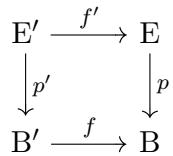
\includegraphics[keepaspectratio]{images/part001_eb35a58e.jpg}}

is a Cartesian square.

Indeed, the map \(h: E' \to B' \times_{B} E\) defined by \(h(x') = (p'(x'), f'(x'))\) is a \(B'\)-morphism of principal fiber bundles, hence an isomorphism; moreover, we have \(pr_{2} \circ h = f'\), whence the result (I, p. 8, prop. 2).

Under the hypotheses of the preceding corollary, one sometimes says that \(f'\) is an f-morphism of principal fiber bundles.

PROPOSITION 2. --- Let (E, p) be a principal fiber bundle with base B and group G, and let \(\varepsilon\) be the section \(b \mapsto (b, e)\) of the trivial principal fiber bundle (B \(\times\) G, \(\mathrm{pr}_{1}\)), where \(e\) denotes the identity element of G. The map \(h \mapsto h \circ \varepsilon\) is a bijection from \(\mathcal{C}_{\mathrm{B}}^{\mathrm{G}}(\mathrm{B} \times \mathrm{G}; \mathrm{E})\) onto the set \(\mathcal{S}(\mathrm{B}; \mathrm{E})\) of continuous sections of \(p\). The inverse bijection associates to a continuous section \(s\) of \(p\) the B-morphism \((b, g) \mapsto s(b) \cdot g\).

COROLLARY. --- A principal fiber bundle is trivializable if and only if it admits a continuous section.

PROPOSITION 3. --- Let E and B be topological spaces, \(p\colon\mathrm{E}\to\mathrm{B}\) a continuous map and G a topological group acting on the right on E. The following conditions are equivalent:

\begin{enumerate}
\def\labelenumi{(\roman{enumi})}
\item
  Endowed with the map p, E is a principal fiber bundle with base B and group G;
\item
  For every \(x \in E\) and every \(g \in G\) , we have \(p(x \cdot g) = p(x)\) , the map \(\theta: (x, g) \mapsto (x, x \cdot g)\) is a homeomorphism of \(E \times G\) onto \(E \times_{B} E\) and every point of B has a neighborhood on which there exists a continuous section of the map p.
\end{enumerate}

(i)⇒(ii): Suppose that (E, p) is a principal fiber bundle. The group G acts continuously and freely on E with the fibers of p as orbits. Consequently, the map \(\theta\) is bijective and continuous. More precisely, if one equips \(E \times_{B} E\) with the action of G defined by \((x, y) \cdot g = (x, y \cdot g)\), the map \(\theta\) is an E-morphism of the trivial principal fiber bundle \(E \times G\) into the principal fiber bundle \((E \times_{B} E \to E, \mathrm{pr}_{1})\) (Example 5), hence an isomorphism (Proposition 1). The other assertions of (ii) follow immediately from the definition.

(ii)⇒(i): Set \(\varphi = pr_{2} \circ \theta^{-1}\) , so that, for every \((x, y) \in E \times_{B} E\) , we have

\[
\theta^ {- 1} (x, y) = (x, \varphi (x, y)).\tag{1}
\]

The map \(\varphi\colon\mathrm{E}\times_{\mathrm{B}}\mathrm{E}\to\mathrm{G}\) is continuous and, for \((x,y)\in\mathrm{E}\times_{\mathrm{B}}\mathrm{E}\), the element \(\varphi(x,y)\) is the unique element \(g\) of G such that \(y=x\cdot g\). Let \(b\) be a point of B; let U be a neighborhood of \(b\) and let \(s\) be a continuous section of \(p\) above U. For \((u,g)\in\mathrm{U}\times\mathrm{G}\), set \(f(u,g)=s(u)\cdot g\); the map \(f\) is a U-morphism from \(U \times G\) to \(\overline{p}^{-1}(\mathrm{U})\). For \(y\in\overline{p}^{-1}(\mathrm{U})\), set \(f'(y)=(p(y),\varphi(s(p(y)),y))\). The map \(f'\) is a U-morphism from \(\overline{p}^{-1}(\mathrm{U})\) to U \(\times\) G. We have

\[
(f \circ f ^ {\prime}) (y) = s (p (y)) \cdot \varphi (s (p (y)), y) = y.
\]

On the other hand, for \((u,g)\in \mathrm{U}\times \mathrm{G}\) , we have

\[
(f ^ {\prime} \circ f) (u, g) = f ^ {\prime} (s (u) \cdot g) = (u, \varphi (s (u), s (u) \cdot g)) = (u, g).
\]

Therefore, f is a U-isomorphism. It follows that \((E,p)\) is a principal fiber bundle with base B and group G.

Remark 1. --- Let (E, p) be a principal fiber bundle with base B and group G. With the notation of Proposition 3, the map \(\theta^{-1}\colon E \times_{B} E \to E \times G\) is a trivialization of the principal fiber bundle \(\mathrm{pr}_{1}\colon E \times_{B} E \to E\). One says that \(\theta^{-1}\) is the canonical trivialization of this principal fiber bundle.

COROLLARY 1. --- Let G be a topological group acting continuously on the right on a topological space E. The following conditions are equivalent:

\begin{enumerate}
\def\labelenumi{(\roman{enumi})}
\item
  The orbit space E/G is Hausdorff, and the space E, equipped with the canonical map \(p: E \rightarrow E/G\), is a principal fiber bundle with group G;
\item
  The group G acts properly (TG, III, p. 27) and freely on E, and every point of E/G has a neighborhood on which there exists a continuous section of the map p.
\end{enumerate}

Set \(B=E/G\). Under each of the hypotheses (i) and (ii), the group G acts continuously and freely on E, so that the map \(\theta\colon(x,g)\mapsto(x,x\cdot g)\) is a continuous bijection from \(E\times G\) onto \(E\times_{B}E\). Let us place ourselves under this hypothesis and denote by \(\varphi\colon E\times_{B}E\to G\) the map \(pr_{2}\circ\theta^{-1}\). Taking formula (1) into account, for \(\theta\) to be a homeomorphism, it is necessary and sufficient that the map \(\varphi\) be continuous. On the other hand, since the equivalence relation defined by G is open (TG, III, p. 10, lemma 2), for the space E/G to be Hausdorff, it is necessary and sufficient that the graph \(E\times_{B}E\) of this equivalence relation be closed in \(E\times E\). For G to act properly on E, it is necessary and sufficient that \(E\times_{B}E\) be closed in \(E\times E\) and that the map \(\varphi\) be continuous. The equivalence of conditions (i) and (ii) then follows from Proposition 3.

COROLLARY 2. --- Let G be a topological group, let H be a subgroup of G, and let p: G → G/H be the canonical map. If the map p admits a continuous section over a nonempty open set of G/H, then p makes G a principal fiber bundle with base G/H and group H.

By left translations, every point of G/H has a neighborhood over which the map p has a continuous section. On the other hand, for \((g,g')\) belonging to \(G\times G\), set \(\varphi(g,g')=g^{-1}g'\). If \(p(g)=p(g')\), \(\varphi(g,g')\) belongs to H. The map \((g,g')\mapsto(g,\varphi(g,g'))\) from \(G\times_{G/H}G\) to \(G\times H\) is continuous and is the inverse of the continuous map \(\theta: G\times H\to G\times_{G/H}G\) defined by \(\theta(g,h)=(g,gh)\), whence the corollary.

Remark 2. --- This situation arises in particular when G is a real Lie group, of finite dimension, countable at infinity, acting transitively and analytically on an analytic manifold X. If one takes for H the stabilizer of a point of X, the map p is a submersion of G onto the homogeneous Lie space G/H, isomorphic to X (LIE, III, p. 109, corollary). It therefore admits local sections (VAR, p. 50).
% semantic-fragments: legacy-input-seam
\relax{}
\subsection{Principal coverings}

DEFINITION 2. --- Let B be a topological space and let G be a group. Endow G with the discrete topology. A principal fiber bundle with base B and group G is called a principal covering of B with group G.

This terminology is legitimate because such a B-space is a covering of B.

A principal G-bundle over a nonempty topological space has a degree, equal to Card G.

PROPOSITION 4. — Let B be a topological space, let (E, p) be a B-space, and let G be a discrete topological group acting on the right on E. The following assertions are equivalent:

\begin{enumerate}
\def\labelenumi{(\roman{enumi})}
\item
  The B-space E is a principal covering with group G;
\item
  For every \(g \in G\) and every \(x \in E\) , we have \(p(x \cdot g) = p(x)\) , the map p induces a homeomorphism from E/G onto B, and the map \(\theta: (x, g) \mapsto (x, x \cdot g)\) is a homeomorphism from E × G onto \(E \times_{B} E\);
\item
  The group G acts continuously and freely on E, the map p is étale, and its fibers are the orbits of G.
\end{enumerate}

(i)⇒(ii): This follows from I, p. 91 and from proposition 3 of I, p. 94. (ii)⇒(iii): Under hypothesis (ii), the action law of G is continuous, and the map p is surjective and open (TG, III, p. 10, lemma 2). Let \(x \in E\) ; the map \(\theta\) induces a bijection from \(\{x\} \times G\) onto \(\{x\} \times p^{-1}(p(x))\) , so the group G acts freely and its orbits are the fibers of p. If e denotes the identity element of G, the diagonal of \(E \times_{B} E\) is the image of \(E \times \{e\}\) by the homeomorphism \(\theta\). Since the group G is discrete, the set \(\{e\}\) is open in G, hence the diagonal \(\Delta_{E}\) is open in \(E \times_{B} E\). By Proposition 7 of I, p. 31, the map p is étale.

(iii)⇒(i): Since every fiber of p is an orbit of the action of G on E, the map p is surjective. As p is étale, for every point b of B, there exists an open neighborhood U of b and a continuous section s of p over U. The set \(s(\mathrm{U})\) is open in E and s induces a homeomorphism from U onto \(s(\mathrm{U})\) (I, p. 30, cor. 3). For every \(g \in G\), the set \(s(\mathrm{U}) \cdot g\) is open in E and the union of these sets over all \(g \in G\) is equal to \(p^{-1}(\mathrm{U})\). If g and \(g'\) are two distinct elements of G, the sets \(s(\mathrm{U}) \cdot g\) and \(s(\mathrm{U}) \cdot g'\) are disjoint, since G acts freely on E. The map \(f: U \times G \to p^{-1}(\mathrm{U})\) defined by \(f(u, g) = s(u) \cdot g\) is continuous for \((u, g) \in U \times G\) and is therefore a homeomorphism from \(U \times G\) onto \(p^{-1}(\mathrm{U})\), compatible with the right action of G. By definition, E is therefore a principal covering of B with group G.

Examples. --- 1) Let E be a topological space, G a discrete topological group acting continuously and freely on E on the right. For the canonical map \(p \colon \mathrm{E} \to \mathrm{E} / \mathrm{G}\) to make E a principal covering of E/G, it is necessary and sufficient that it be étale (condition (iii) of Proposition 4). For example, suppose there exists a topological space X and an étale map \(q \colon \mathrm{E} \to \mathrm{X}\) compatible with the action of G on E; then E is a principal covering of E/G. Indeed, let us denote by \(q' \colon \mathrm{E} / \mathrm{G} \to \mathrm{X}\) the map induced by \(q\); we have \(q = q' \circ p\), and therefore \(p\) is étale by Proposition 6, d) of I, p. 29.

\begin{enumerate}
\def\labelenumi{\arabic{enumi})}
\setcounter{enumi}{1}
\tightlist
\item
  Let \(q \colon \mathrm{E} \to \mathrm{X}\) be a separated étale morphism. The group \(\operatorname{Aut}_{\mathrm{X}}(\mathrm{E})\) , endowed with the discrete topology, acts continuously on the left on E. If the space E is connected, this action is free (I, p. 34, corollary 2). Let G denote the group \(\operatorname{Aut}_{\mathrm{X}}(\mathrm{E})^{\circ}\) and endow E with the right action opposite to that of \(\operatorname{Aut}_{\mathrm{X}}(\mathrm{E})\) . By the preceding example, the space E, endowed with the canonical map \(p \colon \mathrm{E} \to \mathrm{E} / \mathrm{G}\) , is a principal covering with group G.
\end{enumerate}

\subsection{Proper and free actions of discrete groups}

THEOREM 1. --- Let G be a discrete group acting continuously on the right on a topological space E. Suppose that every point of E has a neighborhood U such that U ∩ (U · g) = ∅ for every element g of G other than the identity element. Then the canonical map p: E → E/G makes E a principal covering of E/G with group G.

The action of G on E is free by hypothesis, so it suffices to prove that the map p is étale (I, p. 98, example 1). Let x be a point of E and let U be an open neighborhood of x such that \(U \cap U \cdot g = \varnothing\) for every element g of G distinct from the identity element. The map p is open (TG, III, p. 10, lemma 2) and induces an injective, continuous, and open map from U onto \(p(\mathrm{U})\) , hence a homeomorphism, which proves that the map p is étale.

Examples. --- 1) Let n be an integer \(\geqslant 0\) , let \(\mathbf{P}_{n}(\mathbf{R})\) be the n-dimensional projective space (TG, VI, p. 13) and let \(S_{n}\) be the unit sphere in \(R^{n+1}\) (TG, VI, p. 9). The canonical map from \(S_{n}\) onto \(\mathbf{P}_{n}(\mathbf{R})\) makes \(S_{n}\) a principal covering with group \(\{1,-1\}\) , this group acting by homotheties; the orbits are the pairs of diametrically opposite points.

\begin{enumerate}
\def\labelenumi{\arabic{enumi})}
\setcounter{enumi}{1}
\item
  Every covering of degree 2 has a unique structure of a principal covering with group Z/2Z.
\item
  Let X be a finite-dimensional locally separated differentiable manifold over R, and \(\widetilde{X}\) be the manifold of orientations of the tangent bundle of X (VAR, R, 10.2.4). The space \(\widetilde{X}\) , equipped with its canonical projection onto X, is a principal covering of X with group \(\{1,-1\}\) .
\end{enumerate}

COROLLARY 1. --- Let G be a discrete topological group acting continuously on the right on a topological space E. The following conditions are equivalent:

\begin{enumerate}
\def\labelenumi{(\roman{enumi})}
\item
  The group G acts properly and freely on E;
\item
  The space E/G is Hausdorff, and E is a principal covering with base E/G and group G.
\end{enumerate}

Moreover, under these conditions, the space E is Hausdorff.

Suppose condition (i) is satisfied. Then the spaces E and E/G are separated (TG, III, p. 29, prop. 3), and for every \(x \in \mathrm{E}\) there exists an open neighborhood U of \(x\) in E such that \(\mathrm{U} \cap (\mathrm{U} \cdot g) = \varnothing\) for every element \(g\) of G other than the identity element (TG, III, p. 32, prop. 8). By th. 1, condition (ii) is then satisfied.

The implication (ii)⇒(i) follows from Corollary 1 of I, p. 96.

COROLLARY 2. --- Let G be a topological group and let H be a discrete subgroup of G. Let H act on G by right translations. Then the canonical map from G into the space G/H of left cosets modulo H endows G with a structure of a principal covering of G/H with group H.

Let V be a neighborhood of the identity element \(e\) of G such that \(\mathrm{H} \cap \mathrm{V} = \{e\}\) . There exists an open neighborhood U of \(e\) in G such that \(\mathrm{U}^{-1} \cdot \mathrm{U} \subset \mathrm{V}\) (TG, III, p. 3) and, consequently, \(\mathrm{U} \cap \mathrm{U} \cdot h = \varnothing\) for all \(h \in \mathrm{H}\) , \(h \neq e\) . Corollary 2 of I, p. 100 therefore follows from Theorem 1.

Example 4. --- Equipped with the canonical map from R to T = R/Z (TG, V, p. 2), R is a principal covering of R/Z with group Z.

Remark 1. --- Let G be a separated topological group, K a compact subgroup of G, and H a discrete subgroup of G. The group G acts continuously and properly on the right on the space K\G of right cosets modulo K (TG, III, p. 30, corollary). Since the group H is closed in G, it also acts properly on K\G (TG, III, p. 27, example 1). If, moreover, one has \(H \cap gKg^{-1} = \{e\}\) for all \(g \in G\), the group H acts freely on K\G. The space K\G is then a principal covering with group H of K\G/H by Corollary 1.

COROLLARY 3. --- Let G and G' be topological groups, and let \(\varphi\colon G \to G'\) be a continuous, open, and surjective homomorphism. Suppose that the kernel H of \(\varphi\) is discrete. Then, for the action of H on G by right translations, \(\varphi\) makes G a principal covering of G' with group H.

If moreover the group G is connected, then H is contained in the center of G.

The homomorphism \(\varphi\) induces an isomorphism of topological groups from G/H onto G' (TG, III, p. 16, prop. 24), whence the first assertion by Corollary 2. Suppose the group G is connected. For every \(h \in \mathrm{H}\) , the continuous map from G into H defined by \(g \mapsto ghg^{-1}\) is constant, with value \(h\) . The group H is therefore contained in the center of G.

Remarks. --- 2) Let G and G' be topological groups, and let \(\varphi\colon\mathrm{G}\to\mathrm{G}'\) be a continuous and open homomorphism. If the group G' is connected, the homomorphism \(\varphi\) is surjective. Indeed, \(\varphi(\mathrm{G})\) is an open, hence closed, subgroup of \(\mathrm{G}'\), and consequently is equal to \(\mathrm{G}'\).

\begin{enumerate}
\def\labelenumi{\arabic{enumi})}
\setcounter{enumi}{2}
\tightlist
\item
  Let G be a locally compact group which is countable at infinity, and let G' be a separated topological group whose underlying space is a Baire space. Every continuous surjective homomorphism from G onto G' is open (TG, IX, p. 56, corollary and TG, III, p. 16, prop. 24).
\end{enumerate}

Examples. --- 5) For every integer \(n > 0\), let us denote by \(\mu_{n}\) the group of n-th roots of unity in C (A, V, p. 75). The map \(z \mapsto z^{n}\) makes \(C^{*}\) a principal covering of \(C^{*}\) with group \(\mu_{n}\), this group acting in \(C^{*}\) by multiplication.

\begin{enumerate}
\def\labelenumi{\arabic{enumi})}
\setcounter{enumi}{5}
\tightlist
\item
  Equipped with the map \(z \mapsto e^{2\pi iz}\) (TG, VIII, p. 8, remark), the space C is a principal covering of \(C^{*}\) with group Z. The map \(x \mapsto e^{2\pi ix} = \mathbf{e}(x)\) from R to \(S_{1}\) makes R a principal covering of \(S_{1}\) with group Z.
\end{enumerate}

\subsection{Galois coverings}

DEFINITION 3. --- Let B be a nonempty topological space. A covering E of B is said to be Galois if it is connected and if, for every point b of B, the action of the group \(\mathrm{Aut}_{B}(E)\) of B-automorphisms of E on the fiber \(E_{b}\) is transitive.

Let E be a Galois covering of a topological space B and let p be its projection. The map p is surjective (A, I, p. 56, def. 6), so the space B is connected. Consequently, the covering (E, p) has a degree, which is nonzero.

PROPOSITION 5. --- Let B be a nonempty topological space and let E be a Galois covering of B. The map \((h,x)\mapsto h(x)\) from \(\mathrm{Aut}_{\mathrm{B}}(\mathrm{E})\times\mathrm{E}\) into E is a right action of the group \(\mathrm{Aut}_{\mathrm{B}}(\mathrm{E})^{\circ}\) on E which makes E a principal covering with group \(\mathrm{Aut}_{\mathrm{B}}(\mathrm{E})^{\circ}\) .

Endow the group \(\mathrm{Aut}_{\mathrm{B}}(\mathrm{E})^{\circ}\) with the discrete topology; the operation law \((h,x)\mapsto h(x)\) is then continuous. This action is free (I, p. 34, corollary 2 of proposition 11). Since E is a Galois covering of B, its fibers are the orbits of this action. By proposition 4 of I, p. 97, E is a principal covering with group \(\mathrm{Aut}_{\mathrm{B}}(\mathrm{E})^{\circ}\) .

THEOREM 2. --- Let B be a connected topological space, and let E be a connected, nonempty covering of B. The following properties are equivalent:

\begin{enumerate}
\def\labelenumi{(\roman{enumi})}
\item
  The covering E is Galois.
\item
  There exists a discrete topological group G and a continuous right action of G on E that makes E a principal covering with group G.
\item
  The covering \(E \times_{B} E\) of E defined by the projection \(\mathrm{pr}_{1}\) is trivializable.
\end{enumerate}

When these conditions are satisfied, the canonical map \(G \to \mathrm{Aut}_{B}(E)^{\circ}\) defined by the action of G is an isomorphism of groups.

If, moreover, the space B is locally connected, the preceding properties are equivalent to the following property:

(i') There exists a point b of B such that the action of the group \(\mathrm{Aut}_{\mathrm{B}}(\mathrm{E})\) on the fiber \(E_{b}\) is transitive.

The implication (i)⇒(ii) follows from Proposition 5, and the implication (ii)⇒(iii) from Remark 1 of I, p. 95. Let us prove (iii)⇒(i). Denote by \(p\colon E \to B\) the projection of the covering E. Since B is connected, this covering has a degree, and this degree is nonzero because E is not empty. Let \(b\) be a point of B. Let us prove that the action of \(\mathrm{Aut}_{B}(E)\) on the fiber \(E_{b}\) is transitive. By the preceding, this fiber is nonempty. Let \(x\) and \(x'\) be points of \(E_{b}\). The B-morphisms \(h\colon E \to E\) such that \(h(x) = x'\) correspond bijectively to continuous sections \(s\) of the map \(\mathrm{pr}_{1}\colon E \times_{B} E \to E\) such that \(s(x) = (x, x')\) (I, p. 9, prop. 3). Under hypothesis (iii), such a section exists (I, p. 70, cor. 2) and is unique (I, p. 34, cor. 1 of prop. 11) because the space E is connected. Thus, for every pair \((x, x') \in E \times_{B} E\) there exists a unique B-morphism \(h\colon E \to E\) such that \(h(x) = x'\) . If \(h'\colon E \to E\) is the unique B-morphism such that \(h'(x') = x\) , we have \(h'(h(x)) = x\) and \(h(h'(x')) = x'\) , whence \(h' \circ h = \text{Id}_E\) and \(h \circ h' = \text{Id}_E\) . This proves that \(h\) is a B-automorphism of E. The covering E is therefore Galois.

We have shown that conditions (i), (ii), (iii) are equivalent. Suppose they are satisfied. Let \(\delta\colon\mathbf{G}\to\mathrm{Aut}_{\mathrm{B}}(\mathrm{E})\) be the map which associates with \(g\in\mathrm{G}\) the B-automorphism \(x\mapsto x\cdot g\) of E. The map \(\delta\) is a group homomorphism from G into \(\mathrm{Aut}_{\mathrm{B}}(\mathrm{E})^{\circ}\). Since G acts freely on E, the map \(\delta\) is injective. Let \(h\in\mathrm{Aut}_{\mathrm{B}}(\mathrm{E})\), let \(x\in\mathrm{E}\), and let \(g\) be the unique element of G such that \(x\cdot g=h(x)\).

B-morphisms \(h\) and \(\delta(g)\) coincide at \(x\) and therefore everywhere, since the space E is connected (I, p. 34, cor. 1 of prop. 11), which proves that \(\delta\) is an isomorphism.

Suppose now that the space B is locally connected, and let us prove, under hypothesis (i'), that the covering E is Galois. Let \(E'\) be the quotient space of E by the right action of \(\mathrm{Aut}_{B}(E)^{\circ}\) and denote by \(q\colon E \to E'\) the canonical map. It makes E a surjective covering of E' (I, p. 98, example 2); the map \(p\colon E \to B\) passes to the quotient to define a continuous map \(p'\colon E' \to B\) such that \(p'\circ q = p\) . Since the space B is locally connected, the B-space \((E', p')\) is a covering (I, p. 81, prop. 7). Under hypothesis (i'), there exists a point \(b\) of B such that the fiber \(E'_{b}\) has exactly one element; since the space B is connected, the same holds for every point \(b\) of B (I, p. 74, prop. 4), which proves that E is a Galois covering of B.

PROPOSITION 6. --- Let B be a topological space and G a group. Let (E, p) be a principal covering of B with group G. Suppose the space B is connected and locally connected. Let E₀ be a connected component of E and let G₀ be the subgroup of G stabilizing E₀ (A, I, p. 51). The B-space (E₀, p \textbar{} E₀) is a principal covering for the right action of G₀ on E₀. This covering is Galois.

Since the space B is locally connected, so is E, so that \(E_{0}\) is an open subspace of E (TG, I, p. 85, prop. 11). Since it is also closed (TG, I, p. 83), the space \(E_{0}\) is therefore a covering of B (I, p. 80, cor. 1). Since B is connected, this covering has a degree; since \(E_{0}\) is nonempty, all fibers of \(p|E_{0}\) are therefore nonempty. Let x be a point of \(E_{0}\), and let \(x' \in E_{0}\) such that \(p(x') = p(x)\); there exists an element \(g \in G\) such that \(x \cdot g = x'\). Since the connected components \(E_{0}\) and \(E_{0} \cdot g\) have a common point, they are equal, which implies \(g \in G_{0}\). Thus, the group \(G_{0}\) acts transitively on the fiber of the B-space \(E_{0}\) at \(p(x)\). Proposition 6 follows.

Note. --- If, in Proposition 6, one does not assume the space B to be locally connected, it may happen that the space \(E_{0}\) is not a covering of B (I, p. 147, exerc. 1).

\subsection{Associated fiber bundles}

Let E and F be sets, and let G be a group acting on the right on E and on the left on F. The group G acts on the right on the product \(E \times F\) by the law \((x, y) \cdot g = (x \cdot g, g^{-1} \cdot y)\) , for \(g \in G\) and \((x, y) \in E \times F\) . The quotient set of \(E \times F\) by this operation is denoted \(E \times^{G} F\) .

When E and F are topological spaces, one equips the set \(E \times^{G} F\) with the quotient topology induced by that of \(E \times F\) . The canonical map of \(E \times F\) onto \(E \times^{G} F\) is continuous. If the group G acts continuously on E and F, it is open.

Additionally, let \(F'\) be a set on which G acts on the left, and let \(h: F \to F'\) be a map compatible with the operations of G on F and \(F'\) (A, I, p. 50). The map \(Id_{E} \times h: E \times F \to E \times F'\) is compatible with the operations of G and, by passing to quotients, defines a map denoted \(Id_{E} \times^{G} h\) from \(E \times^{G} F\) into \(E \times^{G} F'\) .

If \(h \colon F \to F'\) is a continuous map (compatible with the operations of G on F and \(F'\) ), the map \(\mathrm{Id}_{\mathrm{E}} \times^{\mathrm{G}} h\) is continuous (TG, I, p. 21, prop. 6).

Examples. --- 1) Let F be a topological space and let G be a topological group acting continuously on the left on F. If one endows the topological space G with the action of G by right translations, the space G × \(^{G}\) F is canonically identified with F as follows. The continuous maps \(\varphi\) : F → G × F and \(\psi\) : G × F → F defined by \(\varphi(f) = (e, f)\) (where e denotes the identity element of G) and \(\psi(g, f) = g \cdot f\) induce continuous maps \(\overline{\varphi}\) : F → G × \(^{G}\) F and \(\overline{\psi}\) : G × \(^{G}\) F → F which are inverses of each other.

\begin{enumerate}
\def\labelenumi{\arabic{enumi})}
\setcounter{enumi}{1}
\item
  Example 1 generalizes as follows. Let B and F be topological spaces and let G be a topological group acting continuously on the left on F. By passing to quotients, the map from B × F to (B × G) × F given by (b, f) ↦ ((b, e), f) and the map from (B × G) × F to B × F given by ((b, g), f) ↦ (b, gf) define B-isomorphisms B × F → (B × G) × \(^{G}\) F and (B × G) × \(^{G}\) F → B × F which are inverses of each other.
\item
  Similarly, let E be a topological space and let G be a topological group acting continuously on the right on E. If the topological space G is endowed with the action of G by left translations, the space \(E \times^{G} G\) is identified with E.
\end{enumerate}

Let E and F be topological spaces, and let G be a topological group acting continuously on the right on E and on the left on F. Let B be a topological space and \(p\colon E \to B\) a continuous map such that \(p(x \cdot g) = p(x)\) for \(x \in E\) and \(g \in G\) . The map \(p \circ pr_{1}\colon E \times F \to B\) defines, by passing to the quotient, a continuous map \(p^{F}\colon E \times^{G} F \to B\) and the canonical map \(\pi\colon E \times F \to E \times^{G} F\) is a B-morphism.

Let B' be a topological space and let \(h\colon B'\to B\) be a continuous map. The group G acts continuously on the right on \(B'\times_{B}E\) by the operation law \(((b',x),g)\mapsto(b',x\cdot g)\). By composing the canonical isomorphism \(((b',x),y)\mapsto(b',(x,y))\) of \((\mathrm{B}'\times_{\mathrm{B}}\mathrm{E})\times\mathrm{F}\) onto \(\mathrm{B}'\times_{\mathrm{B}}(\mathrm{E}\times\mathrm{F})\) and the map \(\operatorname{Id}_{\mathrm{B}'}\times\pi\) from \(\mathrm{B}'\times_{\mathrm{B}}(\mathrm{E}\times\mathrm{F})\) into \(\mathrm{B}'\times_{\mathrm{B}}(\mathrm{E}\times^{\mathrm{G}}\mathrm{F})\), we obtain a continuous map \(\lambda_{0}\colon(\mathrm{B}'\times_{\mathrm{B}}\mathrm{E})\times\mathrm{F}\to\mathrm{B}'\times_{\mathrm{B}}(\mathrm{E}\times^{\mathrm{G}}\mathrm{F})\). By passing to the quotient, it defines a continuous map

\[
\lambda \colon (\mathrm{B} ^ {\prime} \times_ {\mathrm{B}} \mathrm{E}) \times^ {\mathrm{G}} \mathrm{F} \rightarrow \mathrm{B} ^ {\prime} \times_ {\mathrm{B}} (\mathrm{E} \times^ {\mathrm{G}} \mathrm{F}).
\]

Lemma. --- The map λ is a homeomorphism.

The map \(\lambda_0\) is surjective, and two elements of \((\mathrm{B}' \times_{\mathrm{B}} \mathrm{E}) \times \mathrm{F}\) have the same image under \(\lambda_0\) if and only if they belong to the same orbit for the action of G on \((\mathrm{B}' \times_{\mathrm{B}} \mathrm{E}) \times \mathrm{F}\). It follows that the map \(\lambda\) is bijective. Since the map \(\pi\) is open, so is the map \(\mathrm{Id}_{\mathrm{B}'} \times_{\mathrm{B}} \pi\) (I, p. 17, prop. 8), hence so are \(\lambda_0\) and \(\lambda\) (TG, I, p. 32, prop. 3), which proves that \(\lambda\) is a homeomorphism.

PROPOSITION 7. --- Let B be a topological space, let G be a topological group, let (E,p) be a principal fiber bundle over B with group G, and let F be a topological space on which G acts continuously on the left.

\begin{enumerate}
\def\labelenumi{\alph{enumi})}
\item
  The topological space \(E \times^{G} F\) together with the continuous map \(p^{F}: E \times^{G} F \to B\) deduced from the map \(p \circ pr_{1}: E \times F \to B\) by passing to the quotient is a locally trivial fiber bundle of fiber type F; it is trivializable if the B-bundle E is trivializable.
\item
  Let \(\pi\colon\mathrm{E}\times\mathrm{F}\to\mathrm{E}\times^{\mathrm{G}}\mathrm{F}\) be the canonical surjection. The map \(\mu\colon\mathrm{E}\times\mathrm{F}\to\mathrm{E}\times_{\mathrm{B}}(\mathrm{E}\times^{\mathrm{G}}\mathrm{F})\) which associates \((x,\pi(x,f))\) with \((x,f)\) is a homeomorphism whose inverse map is a trivialization of the locally trivial fiber bundle over E \((\mathrm{E}\times_{\mathrm{B}}(\mathrm{E}\times^{\mathrm{G}}\mathrm{F}),\mathrm{pr}_{1})\).
\end{enumerate}

Suppose first that E is the trivial principal fiber bundle \(B \times G\) . By Example 2, the space \(E \times^{G} F\) is then identified with \(B \times F\) and the map \(p^{F}\) with the first projection \(pr_{1}: B \times F \to B\) , which proves that \((\mathrm{E} \times^{\mathrm{G}}\mathrm{F}, p^{\mathrm{F}})\) is a trivializable fiber bundle over B in this case. In the general case, every point of B has a neighborhood U such that the map \(p_{\mathrm{U}}: p^{-1}(\mathrm{U}) \to \mathrm{U}\) makes \(p^{-1}(\mathrm{U})\) a trivializable principal fiber bundle over U. By the preceding, \((p^{-1}(\mathrm{U}) \times^{\mathrm{G}}\mathrm{F} \to \mathrm{U}, (p_{\mathrm{U}})^{\mathrm{F}})\) is a trivializable fiber bundle over U. By the lemma above, applied to the case where \(B' = U\) and \(h: U \to B\) is the canonical injection, the same holds for the U-space \(((p^{\mathrm{F}})^{-1}(\mathrm{U}), (p^{\mathrm{F}})_{\mathrm{U}})\) deduced from \((\mathrm{E} \times^{\mathrm{G}}\mathrm{F}, p^{\mathrm{F}})\) by restriction over U. This proves that \((\mathrm{E} \times^{\mathrm{G}}\mathrm{F}, p^{\mathrm{F}})\) is a locally trivial fiber bundle over B and concludes the proof of assertion a).

The map \(\theta\colon\mathrm{E}\times\mathrm{G}\to\mathrm{E}\times_{\mathrm{B}}\mathrm{E}\) defined by \(\theta(x,g)=(x,x\cdot g)\) is a homeomorphism (I, p. 94, prop. 3) compatible with the operations of G on E \(\times\) G and on E \(\times_{\mathrm{B}}\) E given by \(((x,g),g')\mapsto(x,gg')\) and \(((x,y),g')\mapsto(x,yg')\) respectively. By passing to quotients, \(\theta\) therefore induces a homeomorphism \(\theta'\) from (E \(\times\) G) \(\times^{\mathrm{G}}\) F onto (E \(\times_{\mathrm{B}}\) E) \(\times^{\mathrm{G}}\) F. The map \(\mu\) is the composition of the homeomorphism E \(\times\) F \(\rightarrow\) (E \(\times\) G) \(\times^{\mathrm{G}}\) F (example 2), of \(\theta'\) and of the canonical homeomorphism (E \(\times_{\mathrm{B}}\) E) \(\times^{\mathrm{G}}\) F \(\rightarrow\) E \(\times_{\mathrm{B}}\) (E \(\times^{\mathrm{G}}\) F) (I, p. 105, lemma), whence \(b\) ).

Under the hypotheses of Proposition 7, the locally trivial fiber bundle (E × \(^{G}\) F, p \(^{F}\) ) is called the locally trivial fiber bundle of fiber type F associated with the principal fiber bundle (E, p). All fibers of the B-space E × \(^{G}\) F are homeomorphic to the space F. In particular, if the space F is discrete, the map p \(^{F}\) is a covering.

Examples. --- 4) Let B be a topological space, G a topological group, and let (E, p) be a principal G-bundle over B. Let H be a subgroup of G.

Denote by \(\varphi\colon\mathrm{E}\to\mathrm{E}\times(\mathrm{G}/\mathrm{H})\) and \(\psi\colon\mathrm{E}\times(\mathrm{G}/\mathrm{H})\to\mathrm{E}/\mathrm{H}\) the maps defined by \(\varphi(x)=(x,\mathrm{H})\) and \(\psi(x,g\mathrm{H})=(x\cdot g)\mathrm{H}\) . They are compatible with the projections to B and with the operations of G, and they define, by passing to quotients, morphisms of B-spaces \(\overline{\varphi}\colon\mathrm{E}/\mathrm{H}\to\mathrm{E}\times^{\mathrm{G}}(\mathrm{G}/\mathrm{H})\) and \(\overline{\psi}\colon\mathrm{E}\times^{\mathrm{G}}(\mathrm{G}/\mathrm{H})\to\mathrm{E}/\mathrm{H}\) , inverses of each other. We say that \(\overline{\varphi}\) is the canonical homeomorphism from E/H onto \(\mathrm{E}\times^{\mathrm{G}}(\mathrm{G}/\mathrm{H})\) . In particular, the topological space E/H equipped with the continuous map \(p_{\mathrm{H}}\colon\mathrm{E}/\mathrm{H}\to\mathrm{B}\) is a locally trivial fiber bundle over B with fiber type G/H.

If moreover H is a normal subgroup of G, the action of G endows, by passing to quotients, the B-space E/H with the structure of a principal fiber bundle with group G/H.

In particular, if E is a principal covering of B with group G, then E/H is a covering of B; if H is normal in G, it is a principal covering with group G/H.

\begin{enumerate}
\def\labelenumi{\arabic{enumi})}
\setcounter{enumi}{4}
\item
  Let B be a topological space, let G be a topological group, and let E be a principal G-bundle over B. Let F be a topological homogeneous space with respect to G (TG, III, p. 12). Let y be a point of F, and let \(G_{y}\) be its stabilizer. The map \(\varphi_{y}\colon x\mapsto(x,y)\) from E to \(E\times F\) defines, by passing to the quotient, a homeomorphism \(\overline{\varphi}_{y}\) of \(E/G_{y}\) onto \(E\times^{G}F\) . When the group G is abelian, the subgroup \(G_{y}\) does not depend on the point y, but the homeomorphism \(\overline{\varphi}_{y}\) in general depends on it.
\item
  Let B be a topological space, let G be a topological group, let \((E,p)\) be a principal G-bundle over B. Let H be a topological group and let \(f:G\to H\) be a morphism of topological groups; endow H with the left action of G given by \(g\cdot h=f(g)h\) .
\end{enumerate}

Let \(q \colon \mathrm{E} \times \mathrm{H} \to \mathrm{E} \times^{\mathrm{G}} \mathrm{H}\) be the canonical map; it is open, hence universally strict (I, p. 20, corollary 11). The map \(m \colon (x, h, h') \mapsto q(x, hh')\) from \(\mathrm{E} \times \mathrm{H} \times \mathrm{H}\) into \(\mathrm{E} \times^{\mathrm{G}} \mathrm{H}\) is continuous. Let \((x, h) \in \mathrm{E} \times \mathrm{H}\) , \(h' \in \mathrm{H}\) and \(g \in \mathrm{G}\) ; we have \(m(xg, f(g)^{-1}h, h') = q(xg, f(g)^{-1}hh') = q(x, hh') = m(x, h, h')\) . Consequently, there exists a unique map

\[
m ^ {\prime} \colon (\mathrm{E} \times^ {\mathrm{G}} \mathrm{H}) \times \mathrm{H} \rightarrow \mathrm{E} \times^ {\mathrm{G}} \mathrm{H}
\]

such that \(m'(q(x,h),h') = q(x,hh')\) for all \(x \in E\) and all \(h, h' \in H\) . Since q is universally strict, the map \(m'\) is continuous. This is a right action of the topological group H on the B-space \(E \times^{G} H\) .

Let U be an open subset of B such that \(E_{U}\) is isomorphic to the principal fiber bundle over U \(U \times G\) . Equipped with the operation of H, the U-space \((\mathrm{E} \times^{\mathrm{G}}\mathrm{H})_{\mathrm{U}}\) is identified with the principal fiber bundle \(U \times H\) . This proves that \(E \times^{G}H\) is a principal H-bundle over B.

DEFINITION 4. --- Let B be a topological space and let G be a topological group. A locally trivial fiber bundle X over B is said to be associated with a principal fiber bundle E over B with group G if there exists a topological space F on which the group G acts continuously on the left and a B-isomorphism from E × \(^{G}\) F onto X.

Let E be a principal G-bundle over B, and let X be a locally trivial fiber bundle over B associated with E. If the principal bundle E is trivializable, then X is trivializable (prop. 7). If B' is a topological space and \(h \colon \mathrm{B}' \to \mathrm{B}\) is a continuous map, the locally trivial fiber bundle \(\mathrm{B}' \times_{\mathrm{B}} \mathrm{X}\) deduced from X by base change is associated to the B'-principal fiber bundle \(\mathrm{B}' \times_{\mathrm{B}} \mathrm{E}\) (I, p. 105, lemma).

\subsection{Associated coverings}

Let B be a topological space, let G be a discrete topological group, and let E be a principal covering of B with group G. Let F be a G-set; if F is endowed with the discrete topology, the group G acts continuously on F. The B-space \(E \times^{G} F\) is then a covering. It is called the covering of B with fiber type F associated with the principal covering E.

DEFINITION 5. --- Let B be a topological space, let G be a discrete topological group, and let E be a principal covering of B with group G. A covering X of B is said to be associable to the principal covering E if there exists a G-set F and a B-isomorphism from E × \(^{G}\) F onto X.

Let B be a topological space, let G be a discrete topological group, and let E be a principal covering of B with group G.

For every covering X of B, the group G acts on the left on \(\mathcal{C}_{\mathrm{B}}(\mathrm{E};\mathrm{X})\) by the law defined by \((g\cdot h)(x)=h(x\cdot g)\) for \(x\in E\) , \(g\in G\) , \(h\in\mathcal{C}_{\mathrm{B}}(\mathrm{E};\mathrm{X})\) .

For every G-set F equipped with the discrete topology, define a map \(\alpha_{\mathrm{F}}\colon \mathrm{F}\to \mathcal{C}_{\mathrm{B}}(\mathrm{E};\mathrm{E}\times^{\mathrm{G}}\mathrm{F})\) by:

\[
\alpha_ {\mathrm{F}} (y) (x) = \pi (x, y) \quad \text {for } y \in \mathrm{F} \text { and } x \in \mathrm{E},\tag{2}
\]

where \(\pi\colon\mathrm{E}\times\mathrm{F}\to\mathrm{E}\times^{\mathrm{G}}\mathrm{F}\) is the canonical surjection. The map \(\alpha_{\mathrm{F}}\) is compatible with the operations of G on F and on \(\mathcal{C}_{\mathrm{B}}(\mathrm{E};\mathrm{E}\times^{\mathrm{G}}\mathrm{F})\) .

For every covering X of B, there exists a unique map \(\beta_{X}\) from \(E \times^{G} \mathcal{C}_{B}(E; X)\) into X such that:

\[
\beta_ {\mathrm{X}} (\pi (x, h)) = h (x) \quad \text {for } h \in \mathcal {C} _ {\mathrm{B}} (\mathrm{E}; \mathrm{X}) \text { and } x \in \mathrm{E}.\tag{3}
\]

Indeed, we have \((g^{-1}\cdot h)(x\cdot g)=h(x)\) for \(x\in E\) , \(g\in G\) and \(h\in\mathcal{C}_{\mathrm{B}}(\mathrm{E};\mathrm{X})\) , by definition of the action of G on \(\mathcal{C}_{\mathrm{B}}(\mathrm{E};\mathrm{X})\). When one equips the set \(\mathcal{C}_{\mathrm{B}}(\mathrm{E};\mathrm{X})\) with the discrete topology, the map \(\beta_{X}\) is a B-morphism of coverings.

When \(\mathrm{X} = \mathrm{E}\times^{\mathrm{G}}\mathrm{F}\) , we have

\[
\beta_ {\mathrm{X}} \left(\pi \left(x, \alpha_ {\mathrm{F}} (y)\right)\right) = \pi (x, y) \quad \text {   for   } x \in \mathrm{X} \text {   and   } y \in \mathrm{F}.\tag{4}
\]

PROPOSITION 8. --- Let B be a connected and nonempty topological space. Let G be a discrete group and let (E, p) be a principal covering of B with group G. Suppose that E is connected. With the notations above, we have:

\begin{enumerate}
\def\labelenumi{\alph{enumi})}
\item
  For every G-set F equipped with the discrete topology, the map \(\alpha_{F}\) is an isomorphism of the G-set F onto the G-set \(\mathcal{C}_{\mathrm{B}}(\mathrm{E};\mathrm{E}\times^{\mathrm{G}}\mathrm{F})\) .
\item
  Let X be a covering of B. The B-morphism \(\beta_{X}\) is an isomorphism from \(E \times^{G} \mathcal{C}_{B}(E; X)\) onto X if and only if the covering \((E \times_{B} X, pr_{1})\) of E is trivializable.
\item
  Let \(y\) and \(y'\) be points of F such that \(\alpha_{\mathrm{F}}(y) = \alpha_{\mathrm{F}}(y')\). The space E is not empty; let us choose a point \(x\) in it. We have \(\pi(x, y) = \pi(x, y')\) in \(\mathrm{E} \times^{\mathrm{G}} \mathrm{F}\). Consequently, there exists \(g \in \mathrm{G}\) such that \(x \cdot g = x\) and \(g^{-1} \cdot y = y'\). The first equality implies that \(g\) is the identity element \(e\) of G, hence \(y = y'\). Thus, the map \(\alpha_{\mathrm{F}}\) is injective. On the other hand, let \(h \in \mathcal{C}_{\mathrm{B}}(\mathrm{E}; \mathrm{E} \times^{\mathrm{G}} \mathrm{F})\) and let \(x\) be a point of E. Let \(x' \in \mathrm{E}\) and \(y' \in \mathrm{F}\) be such that \(h(x) = \pi(x', y')\). In particular, \(p(x) = p(x')\); there then exists an element \(g\) of G such that \(x' = x \cdot g\), and one also has \(h(x) = \pi(x, y)\), where we have set \(y = g \cdot y'\). The B-morphisms \(h\) and \(\alpha_{\mathrm{F}}(y)\) coincide at the point \(x\) of E; they are therefore equal since the space E is connected (I, p. 34, cor. 1 of prop. 11), and this proves that the map \(\alpha_{\mathrm{F}}\) is surjective.
\item
  By proposition 7, b) of I, p. 105, applied to F = \(\mathcal{C}_{\mathrm{B}}(\mathrm{E};\mathrm{X})\), the covering \(p^{*}(\mathrm{E}\times^{\mathrm{G}}\mathcal{C}_{\mathrm{B}}(\mathrm{E};\mathrm{X}))\) of E is isomorphic to the trivial covering \(\mathrm{E}\times \mathcal{C}_{\mathrm{B}}(\mathrm{E};\mathrm{X})\). If \(\beta_{\mathrm{X}}\) is an isomorphism, the covering \(p^{*}(\mathrm{X})\) of E is therefore trivializable. Conversely, suppose the covering \(p^{*}(\mathrm{X})\) is trivializable and let us show that the B-morphism \(\beta_{\mathrm{X}}\) is bijective; it will follow that \(\beta_{\mathrm{X}}\) is a B-isomorphism (I, p. 30, cor. 2 of prop. 6).
\end{enumerate}

The map \(\beta_{\mathrm{X}}\) is obtained by passing to the quotient from the map \(\gamma\colon\mathrm{E}\times\mathcal{C}_{\mathrm{B}}(\mathrm{E};\mathrm{X})\to\mathrm{X}\) defined by \(\gamma(x,h)=h(x)\) . Let us show that the map \(\gamma\) is surjective. Let \(x\) be a point of X. The projection of the B-space E is surjective, since it is a principal covering; there therefore exists a point \(y\) of E such that \((y,x)\in\mathrm{E}\times_{\mathrm{B}}\mathrm{X}\) . There then exists a continuous section \(s\) of the trivializable covering \(\mathrm{pr}_{1}:\mathrm{E}\times_{\mathrm{B}}\mathrm{X}\to\mathrm{E}\) such that \(s(y)=(y,x)\) . The map \(h=\mathrm{pr}_{2}\circ s:\mathrm{E}\to\mathrm{X}\) is a B-morphism and one has \(h(y)=x\) , whence the surjectivity of the map \(\gamma\) and, consequently, that of the map \(\beta_{\mathrm{X}}\) .

Let us finally show that \(\beta_{\mathrm{X}}\) is injective. Let \((x,h)\) and \((x^{\prime},h^{\prime})\) be elements of \(\mathrm{E}\times \mathcal{C}_{\mathrm{B}}(\mathrm{E};\mathrm{X})\) such that \(h(x) = h'(x')\) . Note that \(x\) and \(x'\) have the same projection in B; there therefore exists an element \(g\) of G such that \(x' = x\cdot g\) . One then has \(h(x) = h'(x\cdot g) = (g\cdot h')(x)\) . Since the space E is connected, one has \(h = g\cdot h'\) (I, p. 34, cor. 1 of prop. 11). Thus, \((x,h)\) and \((x',h')\) have the same class in \(\mathrm{E}\times^{\mathrm{G}}\mathcal{C}_{\mathrm{B}}(\mathrm{E};\mathrm{X})\) , which shows that the map \(\beta_{\mathrm{X}}\) is injective, which completes the proof.

COROLLARY 1. --- Let (E,p) be a principal covering of B with group G; suppose that E is connected and nonempty. A covering X of B is associable to E if and only if the covering \(p^{*}(X)\) is trivializable.

If the covering \(p^{*}(\mathrm{X})\) is trivializable, it follows from Proposition 8, b), that the covering X is associable to E. In this case, the map \(\beta_{X}\) identifies the covering X with the fiber-type covering \(\mathcal{C}_{\mathrm{B}}(\mathrm{E};\mathrm{X})\) associated with E. Conversely, let F be a G-set equipped with the discrete topology, and suppose that we have \(X = E \times^{G} F\) . Then, \(\alpha_{F}\) is an isomorphism (loc. cit., a)) and formula (4) implies that \(\beta_{X}\) is an isomorphism. Consequently, the covering \(p^{*}(\mathrm{X})\) is trivializable (prop. 8, b)), whence the corollary.

COROLLARY 2. --- Let B be a connected and locally connected topological space, let (E,p) be a principal covering of B with group G. Let E₀ be a connected component of E and let G₀ be the subgroup of G stabilizing E₀. The B-space (E₀, p \textbar{} E₀) is a principal covering with group G₀ (I, p. 103, prop. 6).

Every covering X of B that is associable to the principal covering E is associable to the principal covering \(E_{0}\). In particular, the covering E is associated with the principal covering \(E_{0}\).

Indeed, if the covering X is associable to E, the covering \(p^{*}(\mathrm{X})\) is trivializable and the covering \(p_{0}^{*}(\mathrm{X})\) induced by \(p^{*}(\mathrm{X})\) over \(E_{0}\) is therefore trivializable.

More precisely, note that the map \((x,g)\mapsto x\cdot g\) from \(E_{0}\times G\) into E induces, by passing to the quotient, a B-isomorphism of principal coverings from \(E_{0}\times^{G_{0}}G\) onto E.

PROPOSITION 9. --- Let B be a topological space, let E be a principal covering of B with group G, connected and nonempty. Let F be a nonempty G-set equipped with the discrete topology. For the space E × \(^{G}\) F to be connected, it is necessary and sufficient that G acts transitively on F.

Let U be an open and closed subset of \(E \times^{G} F\) . If \(\pi: E \times F \to E \times^{G} F\) denotes the canonical surjection, \(\pi^{-1}(U)\) is an open and closed subset of \(E \times F\) which is stable under G. Since E is connected, there exists a subset \(F' \subset F\), stable under G, such that \(\pi^{-1}(U) = E \times F'\), whence \(U = \pi(E \times F')\). Let \(F'\) and \(F''\) be subsets of F stable under G such that \(\pi(E \times F') = \pi(E \times F'')\). Since E is not empty, we have \(F' = F''\). The map \(F' \mapsto \pi(E \times F')\) is a bijection from the set of G-stable subsets of F onto the set of clopen subsets of \(E \times^{G} F\). The proposition follows.

PROPOSITION 10. --- Let B be a topological space, let (E,p) be a principal covering of B with group G, and let X be a covering of B. Suppose that E and X are connected and nonempty. The following properties are equivalent:

\begin{enumerate}
\def\labelenumi{(\roman{enumi})}
\item
  The covering X is associated to the principal covering E;
\item
  There exists a subgroup H of G such that X is B-isomorphic to E/H;
\item
  There exists a surjective B-morphism \(h: \mathrm{E} \to \mathrm{X}\) ;
\item
  For every point \((y, x)\) of \(E \times_{B} X\) there exists a B-morphism \(r: E \to X\) such that \(r(y) = x\) .
\end{enumerate}

Suppose these conditions are satisfied, and let H be a subgroup of G such that X is B-isomorphic to E/H. The covering X is Galois if and only if the subgroup H is normal in G.

(i)⇒(ii): Let F be a discrete G-set such that the covering \(E \times^{G} F\) is B-isomorphic to X. The set F is nonempty and the space \(E \times^{G} F\) is connected, hence the group G acts transitively on F (prop. 9). Then, the space \(E \times^{G} F\) is B-isomorphic to E/H, where H is the subgroup of G fixing a point of F (I, p. 106, example 4).

(ii)⇒(iii): Indeed, the canonical surjection from E onto E/H is a surjective B-morphism.

(iii)⇒(iv): Let \((y, x)\) be a point of \(E \times_{B} X\). Since the map h is surjective, there exists a point \(y'\) of E such that \(h(y') = x\). The points y and \(y'\) have the same projection in B. Since the covering E is principal with group G, there exists \(g \in G\) such that \(y \cdot g = y'\). The map \(r: E \to X\) defined by \(z \mapsto h(z \cdot g)\) is a B-morphism and one has \(r(y) = x\).

(iv)⇒(i): Since X is nonempty and the projection of E onto B is surjective, the space \(E \times_{B} X\) is not empty. There therefore exists a B-morphism r from E to X. The map ( \(Id_{E}, r\) ): \(E \to E \times_{B} X\) is a section of the covering \(p^{*}(X)\) of E. Since the space E is connected, it follows from Corollary 2 of Prop. 1 in I, p. 69 that the covering \(p^{*}(X)\) is trivializable, which proves that the covering X is associable to the Galois covering p (Proposition 8).

Suppose now that these conditions are satisfied. Let X denote the B-space E/H, q its projection, and \(h: E \rightarrow E/H\) the canonical map.

If the group H is normal in G, then X is a principal covering with group G/H (I, p. 106, example 4). Since X and B are connected and nonempty, X is a Galois covering of B (I, p. 102, th. 2). Conversely, suppose that E/H is a Galois covering of B and let K = Aut \(_{B}\) (E/H) \(^{\circ}\) . We define a map \(\alpha: \mathrm{E} \times \mathrm{G} \to \mathrm{K}\) by associating with \((t, g) \in \mathrm{E} \times \mathrm{G}\) the unique element \(k\) of K such that \(h(t \cdot g) = h(t) \cdot k\) . It is continuous because it is obtained by composing the continuous map \((t, g) \mapsto (h(t), h(t \cdot g))\) from E \(\times\) G into X \(\times_{\mathrm{B}}\) X with the canonical trivialization (I, p. 95, remark 1) X \(\times_{\mathrm{B}}\) X \(\to\) X \(\times\) K of \(q^{*}(\mathrm{X})\) . Since E is connected and K is a discrete group, the continuous map \(t \mapsto \alpha(t, g)\) is constant for every \(g \in \mathrm{G}\); we denote its value by \(\alpha(g)\). If \(t \in \mathrm{E}\), \(g \in \mathrm{G}\), and \(g' \in \mathrm{H}\), we then have

\[
h (t) = h \left(t \cdot g ^ {- 1} g\right) = h \left(t \cdot g ^ {- 1}\right) \cdot \alpha (g) = h \left(t \cdot g ^ {- 1} \cdot g ^ {\prime}\right) \cdot \alpha (g) = h \left(t \cdot \left(g ^ {- 1} g ^ {\prime} g\right)\right).
\]

It follows that \(g^{-1}g'g\) belongs to H, and therefore H is normal in G.

COROLLARY. --- Let E be a Galois covering of B and let X be a covering of B, connected and nonempty. Suppose that X is a finite covering or that the space B is locally connected. If there exists a B-morphism h: E → X, then the covering X is associated with the principal covering E.

In both cases, the B-morphism h is a covering (I, p. 77, cor. 3 of th. 1, and I, p. 78, prop. 5), and a nonempty covering of a connected space is surjective (I, p. 68).

THEOREM 3. --- Let B be a nonempty, connected, and locally connected topological space. Every covering of B can be associated with a Galois covering; every finite covering of B can be associated with a finite Galois covering.

Let X be a covering of B, and denote its projection by q. Since the space B is connected and nonempty, the covering X has a degree; denote this degree by F and endow the set F with the discrete topology. Since the space B is locally connected, the sheaf \(\mathcal{I} = \underline{\mathcal{I}som}_{\mathrm{B}}(\mathrm{B} \times \mathrm{F}; \mathrm{X})\) is locally constant, and at every point b of B, its stalk \(I_{b}\) is canonically isomorphic to the set \(\mathcal{B}(\mathrm{F}; \mathrm{X}_{b})\) of bijections from F onto the fiber \(X_{b}\) (I, p. 89, prop. 12). Let \(E = E_{\mathcal{I}}\) be the associated covering (I, p. 86, corollary).

Let G be the group of permutations of F. For every \(g \in G\), we define a morphism \(\gamma'(g)\) of the sheaf \(\mathcal{I}\) into itself as follows: for every open set U of B, the map \(\gamma'(g)_{\mathrm{U}}\) associates to a U-isomorphism \(\varphi: \mathrm{U} \times \mathrm{F} \to q^{-1}(\mathrm{U})\) the U-isomorphism defined by \((b, f) \mapsto \varphi(b, g(f))\) for \(b \in U\) and \(f \in F\). We have \(\gamma'(\mathrm{Id}_{\mathrm{F}}) = \mathrm{Id}_{\mathcal{I}}\) and \(\gamma'(g \circ g') = \gamma'(g') \circ \gamma'(g)\), for \(g, g' \in G\), so that for every \(g \in G\), \(\gamma'(g)\) is an automorphism of the sheaf \(\mathcal{I}\). The B-morphism \(\gamma(g): E \to E\) associated with \(\gamma'(g)\) is an automorphism (I, p. 50). If \(x = [\mathrm{U}, \varphi, b]\) is an element of E, where U is an open subset of B, b a point of U, and \(\varphi\) a U-isomorphism from U×F to \(q^{-1}(\mathrm{U})\), we have \(\gamma(g)(x) = [\mathrm{U}, \psi, b]\), where \(\psi\) is defined by \(\psi(a, f) = \varphi(a, g(f))\), for \(a \in U\) and \(f \in F\). If g and \(g'\) are elements of G, we have \(\gamma(g \circ g') = \gamma(g') \circ \gamma(g)\). We have \(\gamma(\mathrm{Id}_{\mathrm{F}}) = \mathrm{Id}_{\mathrm{E}}\). We thus define a continuous right action of G on E by setting \(x \cdot g = \gamma(g)(x)\), for \(x \in E\) and \(g \in G\). The group G acts simply transitively on every fiber of E, so that the covering E equipped with this action is a principal covering with group G (I, p. 97, prop. 4). Let h be the map from E × F to X defined by \(h([\mathrm{U}, \varphi, b], f) = \varphi(b, f)\) for every open subset U of B, every point b of U, and every U-isomorphism \(\varphi\) from U × F onto \(q^{-1}(\mathrm{U})\). By definition of the topology on E, it is continuous; it is a B-morphism. For every element g of G and every point \((x, f)\) of E × F, we have \(h(x, g(f)) = h(x \cdot g, f)\). The map h therefore defines, by passing to the quotient, a B-morphism \(h': E \times^{G} F \to X\). For every point \(b\) of B, the map \(h_b\colon \mathrm{E}_b\times \mathrm{F}\to \mathrm{X}_b\) is identified with the map \((\varphi, f)\mapsto \varphi(f)\) from \(\mathcal{B}(\mathrm{F};\mathrm{X}_b)\times \mathrm{F}\) into \(\mathrm{X}_b\), so that the map \(h_b^\prime\) is bijective. Consequently, \(h^\prime\) is a B-isomorphism from \(\mathrm{E}\times^{\mathrm{G}}\mathrm{F}\) onto X (I, p. 30, cor. 2 of prop. 6).

Since the space B is connected, locally connected, and nonempty, the covering X, associable to the principal covering E, is associable to a Galois covering (I, p. 110, corollary 2). If the covering X is finite, then so is the covering E, hence X is associable to a finite Galois covering (loc. cit.).

\subsection{Principal fiber bundles defined by cocycles}

DEFINITION 6. --- Let B be a topological space, let G be a topological group, and let \(\mathcal{U} = (\mathrm{U}_{i})_{i\in \mathrm{I}}\) be an open covering of B. A continuous 1-cocycle on B with values in G, subordinate to \(\mathcal{U}\), is the data, for every pair \((i,j)\) of elements of I, of a continuous map \(g_{i,j}\) from \(\mathrm{U}_i\cap \mathrm{U}_j\) into G, such that for every triple \((i,j,k)\in \mathrm{I}\times \mathrm{I}\times \mathrm{I}\) and every point b of \(\mathrm{U}_i\cap \mathrm{U}_j\cap \mathrm{U}_k\), one has

\[
g _ {i, k} (b) = g _ {i, j} (b) g _ {j, k} (b).
\]

We denote \(Z_{\mathrm{cont}}^{1}(\mathrm{B},\mathcal{U},\mathrm{G})\) the set of continuous 1-cocycles on B with values in G, subordinate to the covering U.

In this issue, we will simply say cocycle instead of continuous 1-cocycle.

Let \((\mathrm{E},p)\) be a principal G-bundle over B and let \(\mathcal{U} = (\mathrm{U}_{i})_{i\in\mathrm{I}}\) be a covering of B by open sets \(U_{i}\). We say that E is trivializable over U if, for every \(i\in I\), E is trivializable over \(U_{i}\). We then call a U-trivialization of E a family \((f_{i})_{i\in\mathrm{I}}\), where \(f_{i}\colon p^{-1}(\mathrm{U}_{i})\to\mathrm{U}_{i}\times\mathrm{G}\) is a trivialization of E over \(U_{i}\).

Let \(\mathcal{U} = (\mathrm{U}_i)_{i\in \mathrm{I}}\) be a covering of B by open sets, and let \((\mathrm{E},p)\) be a principal G-bundle over B equipped with a \(\mathcal{U}\)-trivialization \((f_i)_{i\in \mathrm{I}}\). For every pair \((i,j)\in \mathrm{I}\times \mathrm{I}\), denote by \(g_{ij}\) the map from \(\mathrm{U}_i\cap \mathrm{U}_j\) into G defined by

\[
(b, g _ {i j} (b)) = f _ {i} \circ f _ {j} ^ {- 1} (b, e),
\]

where e denotes the identity element of G. It is continuous.

Since \(f_{i}\) and \(f_{j}\) are compatible with the operations of G, we have

\[
(f _ {i} \circ f _ {j} ^ {- 1}) (b, g) = (b, g _ {i j} (b) g)
\]

for \(b \in \mathrm{U}_i \cap \mathrm{U}_j\) and \(g \in \mathrm{G}\). If \(b\) is a point of \(\mathrm{U}_i \cap \mathrm{U}_j \cap \mathrm{U}_k\) (where \(i, j, k \in \mathrm{I}\)), we have

\[
(f _ {i} \circ f _ {k} ^ {- 1}) (b, e) = (b, g _ {i k} (b))
\]

and

\[
\begin{array}{c} (f _ {i} \circ f _ {k} ^ {- 1}) (b, e) = (f _ {i} \circ f _ {j} ^ {- 1}) \circ (f _ {j} \circ f _ {k} ^ {- 1}) (b, e) \\ = (f _ {i} \circ f _ {j} ^ {- 1}) (b, g _ {j k} (b)) = (b, g _ {i j} (b) g _ {j k} (b)). \end{array}
\]

It follows that

\[
g _ {i k} (b) = g _ {i j} (b) g _ {j k} (b),
\]

so that the family \((g_{ij})\) is a cocycle on B with values in G, subordinate to the covering U. It is called the cocycle defined by the family of trivializations \((f_{i})_{i\in\mathrm{I}}\).

Let B, G, and U be as in Definition 6, and let \((g_{ij}) \in Z_{\mathrm{cont}}^{1}(\mathrm{B}, \mathcal{U}, \mathrm{G})\) be a cocycle. For every pair \((i, j) \in \mathrm{I} \times \mathrm{I}\), the map \(\gamma_{ij} \colon (\mathrm{U}_{i} \cap \mathrm{U}_{j}) \times \mathrm{G} \to (\mathrm{U}_{i} \cap \mathrm{U}_{j}) \times \mathrm{G}\) defined by

\[
\gamma_ {i j} (b, g) = \left(b, g _ {i j} (b) g\right) \quad \text {   for   } b \in \mathrm{U} _ {i} \cap \mathrm{U} _ {j} \text {   and   } g \in \mathrm{G}\tag{5}
\]

is an isomorphism of principal bundles over the base \(U_{i} \cap U_{j}\) . For every triple \((i,j,k) \in \mathrm{I} \times \mathrm{I} \times \mathrm{I}\) and every pair \((b,g) \in (\mathrm{U}_{i} \cap \mathrm{U}_{j} \cap \mathrm{U}_{k}) \times \mathrm{G}\) , we have:

\[
\gamma_ {i k} (b, g) = \gamma_ {i j} \circ \gamma_ {j k} (b, g).
\]

Let F be the topological space obtained by gluing together the spaces \(U_{i} \times G\) along the \((\mathrm{U}_{i} \cap \mathrm{U}_{j}) \times \mathrm{G}\) by means of the bijections \(\gamma_{ij}\) (TG, I, p. 16). For every \(i \in I\), the image of \(U_{i} \times G\) in F is an open set of F (TG, I, p. 17, prop. 9). The canonical projections \(p_{i}: U_{i} \times G \to U_{i}\) glue together into a continuous map p from F to B. The maps \(\gamma_{ij}\) being compatible with the right G-operations in the spaces \(U_{i} \times G\), one deduces a continuous right action of G on F which makes F a principal fiber bundle with base B and group G, equipped with a trivialization over each \(U_{i}\). We say that F is the principal fiber bundle defined by the cocycle \((g_{ij})\).

DEFINITION 7. --- Let B be a topological space, let G be a topological group, and let \(\mathcal{U} = (\mathrm{U}_{i})_{i\in \mathrm{I}}\) be an open covering of B. We say that two cocycles \((g_{ij})\) and \((g_{ij}^{\prime})\) in \(\mathrm{Z}_{\mathrm{cont}}^{1}(\mathrm{B},\mathcal{U},\mathrm{G})\) are cohomologous if there exists a family \((h_{i})_{i\in\mathrm{I}}\) of continuous maps \(h_{i}\colon U_{i}\to G\) such that one has

\[
g _ {i j} ^ {\prime} (b) = h _ {i} (b) g _ {i j} (b) h _ {j} (b) ^ {- 1}\tag{6}
\]

for every pair \((i,j)\in \mathrm{I}\times \mathrm{I}\) and every \(b\in \mathrm{U}_i\cap \mathrm{U}_j\).

The relation “\((g_{ij})\) is cohomologous to \((g'_{ij})\)” is an equivalence relation on the set \(Z_{\mathrm{cont}}^{1}(\mathrm{B},\mathcal{U},\mathrm{G})\). We denote by \(H_{\mathrm{cont}}^{1}(\mathrm{B},\mathcal{U},\mathrm{G})\) the quotient set of \(Z_{\mathrm{cont}}^{1}(\mathrm{B},\mathcal{U},\mathrm{G})\) by this equivalence relation.

PROPOSITION 11. --- Let B be a topological space, G a topological group, and \(\mathcal{U} = (\mathrm{U}_{i})_{i\in \mathrm{I}}\) an open covering of B.

\begin{enumerate}
\def\labelenumi{\alph{enumi})}
\item
  Every principal G-bundle over B that is trivializable over U is isomorphic to a principal bundle defined by a cocycle in \(Z_{\mathrm{cont}}^{1}(\mathrm{B}, \mathcal{U}, \mathrm{G})\).
\item
  Let (E, p) and (E', p') be principal G-bundles over B that are trivializable over U. Let \((f_i)_{i \in I}\) (resp. \((f_i')_{i \in I}\)) be a trivialization of (E, p) (resp. of \((E', p')\)) adapted to U, and denote by \((g_{ij})_{(i,j) \in I \times I}\) (resp. \((g_{i,j}')_{(i,j) \in I \times I}\)) the cocycle defined by this trivialization. Then, the principal fiber bundles (E, p) and (E', p') are isomorphic if and only if these cocycles are cohomologous.
\end{enumerate}

Let us prove \(b\). Let \(\varphi: \mathrm{E} \to \mathrm{E}'\) be an isomorphism of principal bundles with base B and group G. For every \(i \in \mathrm{I}\), let \(h_i\) be the continuous map from \(\mathrm{U}_i\) into G defined by

\[
(b, h _ {i} (b)) = f _ {i} ^ {\prime} \circ \varphi \circ f _ {i} ^ {- 1} (b, e).
\]

Since, for every \(i \in I\) , \(f_{i}\) and \(f_{i}^{\prime}\) are compatible with the operations of G, we have for every \(b \in U_{i}\) and every \(g \in G\) ,

\[
(f _ {i} ^ {\prime} \circ \varphi \circ f _ {i} ^ {- 1}) (b, g) = (b, h _ {i} (b) g)
\]

and

\[
(f _ {i} \circ \varphi^ {- 1} \circ (f _ {i} ^ {\prime}) ^ {- 1}) (b, g) = (b, h _ {i} (b) ^ {- 1} g).
\]

Consequently, for every pair \((i,j)\in \mathrm{I}\times \mathrm{I}\) and every point \(b\) of \(\mathrm{U}_i\cap \mathrm{U}_j\),

\[
\begin{array}{c} f _ {i} ^ {\prime} \circ (f _ {j} ^ {\prime}) ^ {- 1} (b, e) = (f _ {i} ^ {\prime} \circ \varphi \circ f _ {i} ^ {- 1}) \circ (f _ {i} \circ f _ {j} ^ {- 1}) \circ (f _ {j} \circ \varphi^ {- 1} \circ (f _ {j} ^ {\prime}) ^ {- 1}) (b, e) \\ = (b, h _ {i} (b) g _ {i j} (b) h _ {j} (b) ^ {- 1}) \end{array}
\]

so that we have

\[
g _ {i j} ^ {\prime} (b) = h _ {i} (b) g _ {i j} (b) h _ {j} (b) ^ {- 1}.
\]

This proves that the cocycles \((g_{ij})\) and \((g'_{ij})\) are cohomologous.

Conversely, suppose that these cocycles are cohomologous, and let \((h_{i})_{i\in\mathrm{I}}\) be a family of continuous maps \(h_{i}\colon U_{i}\to G\) such that one has \(g_{ij}^{\prime}(b)=h_{i}(b)g_{ij}(b)h_{j}(b)^{-1}\) for \(i,j\in I\) and \(b\in U_{i}\cap U_{j}\). For \(i\in I\), let \(\varphi_{i}\colon p^{-1}(U_{i})\to(p')^{-1}(U_{i})\) be the map defined by \(f_{i}^{\prime}\circ\varphi_{i}\circ f_{i}^{-1}(b,g)=(b,h_{i}(b)g)\), for \(b\in U_{i}\) and \(g\in G\). This is an isomorphism of principal fiber bundles with base \(U_{i}\) and group G. For \((i,j)\in I\times I\), denote by \(\gamma_{ij}\) and \(\gamma_{ij}^{\prime}\) the gluing homeomorphisms associated as above to the cocycles \((g_{ij})\) and \((g_{ij}^{\prime})\), respectively (I, p. 115, formula (5)), so that \(f_{i}(b,g)=\gamma_{ij}\circ f_{j}(b,g)\) and \(f_{i}^{\prime}(b,g)=\gamma_{ij}^{\prime}\circ f_{j}^{\prime}(b,g)\) for all \((b,g)\in(U_{i}\cap U_{j})\times G\). Consequently, for \((i,j)\in I\times I\) and \((b,g)\in(U_{i}\cap U_{j})\times G\), we have the relations

\[
\begin{array}{r l} & f _ {i} ^ {\prime} \circ \varphi_ {j} \circ f _ {i} ^ {- 1} (b, g) = \gamma_ {i j} ^ {\prime} \circ (f _ {j} ^ {\prime} \circ \varphi_ {j} \circ f _ {j} ^ {- 1}) (b, g _ {i j} (b) ^ {- 1} g) \\ & \qquad = \gamma_ {i j} ^ {\prime} (b, h _ {j} (b) g _ {i j} (b) ^ {- 1} g) \\ & \qquad = (b, g _ {i j} ^ {\prime} (b) h _ {j} (b) g _ {i j} (b) ^ {- 1} g) \\ & \qquad = (b, h _ {i} (b) g) = f _ {i} ^ {\prime} \circ \varphi_ {i} \circ f _ {i} ^ {- 1} (b, g). \end{array}
\]

This demonstrates that \(\varphi_{i}\) and \(\varphi_{j}\) coincide on \(p^{-1}(\mathrm{U}_{i}\cap\mathrm{U}_{j})\). The morphisms \(\varphi_{i}\) therefore glue together into a B-morphism of principal bundles from E to E'. The assertion \(b\) follows because any morphism of principal bundles with base B and group G is an isomorphism (I, p. 93, prop. 1).

Now let us prove \(a\). Let \((\mathrm{E}, p)\) be a principal fiber bundle with structure group G, equipped, for every \(i \in \mathrm{I}\), with a trivialization \(f_i: p^{-1}(\mathrm{U}_i) \to \mathrm{U}_i \times \mathrm{G}\) over \(\mathrm{U}_i\). Let \((g_{ij})\) be the cocycle defined by this family, and let F be the principal fiber bundle defined by the cocycle \((g_{ij})\). By construction, the principal fiber bundle F is equipped with a trivialization over \(\mathcal{U}\); this trivialization defines the cocycle \((g_{ij})\). By assertion \(b\), the principal fiber bundle \((\mathrm{E}, p)\) is isomorphic to F.

Let B be a topological space and G a topological group. Let \((E,p)\) be a principal fiber bundle with base B and group G. Let s be a section of the surjective map p (E, II, p. 19, prop. 8). The map \(f\colon B\times G\to E\) defined by \(f(b,g)=s(b)\cdot g\) is a bijection compatible with the action of G. Equip \(B\times G\) with the topology obtained by transport of structure; \((B\times G,\mathrm{pr}_{1})\) is then a principal fiber bundle with base B and group G isomorphic to E. There therefore exists a set T of principal bundles with base B and group G such that every principal fiber bundle with base B and group G is isomorphic to an element of T. Let P(B, G) denote the set of isomorphism classes of principal bundles with base B and group G (E, II, p. 47).

Let \(\mathcal{U} = (\mathrm{U}_i)_{i\in \mathrm{I}}\) be an open cover of B. Let us denote by \(\mathrm{P(B,\mathcal{U},G)}\) the subset of \(\mathrm{P(B,G)}\) consisting of the isomorphism classes of principal bundles that are trivializable over \(\mathcal{U}\). By Proposition 11, there exists a map \(r_{\mathcal{U}}\) from \(\mathrm{H}_{\mathrm{cont}}^{1}(\mathrm{B},\mathcal{U},\mathrm{G})\) into \(\mathrm{P(B,\mathcal{U},G)}\) which associates with the class of a cocycle \((g_{ij})\in Z_{\mathrm{cont}}^{1}(\mathrm{B},\mathcal{U},\mathrm{G})\) the isomorphism class of the principal bundle defined by this cocycle; it is a bijection (loc. cit.). The inverse bijection \(s_{\mathcal{U}}\) associates with the isomorphism class in \(\mathrm{P(B,\mathcal{U},G)}\) of a principal fiber bundle E, trivializable over \(\mathcal{U}\), the class of the cocycle defined by any family of trivializations of E over \(\mathcal{U}\). In this correspondence, the isomorphism class of the trivial principal fiber bundle \(\mathrm{B}\times \mathrm{G}\) corresponds to the cohomology class of the constant cocycle \(g_{ij} = e\), also called the trivial cocycle.

By virtue of the definition of a principal fiber bundle, the set P(B, G) is the union of the sets of the form P(B, U, G), where U is an open covering of B.

Let \(\mathcal{U} = (\mathrm{U}_i)_{i\in \mathrm{I}}\) be an open cover of B and let \(\mathcal{V} = (\mathrm{V}_k)_{k\in \mathrm{K}}\) be an open cover of B finer than \(\mathcal{U}\). We have \(\mathrm{P(B,\mathcal{U},G)}\subset\) \(\mathrm{P(B,\mathcal{V},G)}\); we denote by \(i_{\mathcal{V}\mathcal{U}}\) the canonical injection defined by this inclusion. Let us choose a map \(\varphi \colon \mathrm{K}\to \mathrm{I}\) such that \(\mathrm{V}_k\subset \mathrm{U}_{\varphi (k)}\) for all \(k\in \mathrm{K}\). Given a cocycle \((g_{ij})\in \mathrm{Z}_{\mathrm{cont}}^1 (\mathrm{B},\mathcal{U},\mathrm{G})\), set, for every pair \((k,\ell)\in \mathrm{K}\times \mathrm{K}\), \(\overline{g}_{k\ell} = g_{\varphi (k)\varphi (\ell)}\mid \mathrm{V}_k\cap \mathrm{V}_\ell\).

The family \((\overline{g}_{k\ell})\) is a cocycle on B, with values in G, subordinate to V. If \((g'_{ij}) \in \mathrm{Z}_{\mathrm{cont}}^{1}(\mathrm{B}, \mathcal{U}, \mathrm{G})\) is a cocycle cohomologous to the cocycle \((g_{ij})\), the cocycle \((\overline{g}'_{k\ell})\) deduced from \((g'_{ij})\) is cohomologous to the cocycle \((\overline{g}_{k\ell})\). This yields a map

\[
c (\varphi) \colon \mathrm{H} _ {\mathrm{cont}} ^ {1} (\mathrm{B}, \mathcal {U}, \mathrm{G}) \to \mathrm{H} _ {\mathrm{cont}} ^ {1} (\mathrm{B}, \mathcal {V}, \mathrm{G})
\]

which to the class of \((g_{ij})\) associates the class of \((\overline{g}_{k\ell})\) .

Let E be a principal fiber bundle with base B and group G and, for every \(i \in I\), let \(f_i: E_{U_i} \to U_i \times G\) be a trivialization of the \(U_i\)-principal fiber bundle \(E_{U_i}\). For all \(k \in K\), let \(f_k' : E_{V_k} \to V_k \times G\) be the trivialization deduced from \(f_{\varphi(k)}\) by passing to subsets. Let \((g_{ij}) \in Z_{\mathrm{cont}}^1(\mathrm{B}, \mathcal{U}, \mathrm{G})\) be the cocycle defined by the family \((f_i)\); the cocycle defined by the family \((f_{k}^{\prime})\) is precisely the cocycle \((\overline{g}_{k\ell})\) defined above. Thus, the following diagram is commutative:

\[
\begin{array}{c} \mathrm{H} _ {\mathrm{cont}} ^ {1} (\mathrm{B}, \mathcal {U}, \mathrm{G}) ^ {c (\varphi)} \longrightarrow \mathrm{H} _ {\mathrm{cont}} ^ {1} (\mathrm{B}, \mathcal {V}, \mathrm{G}) \\ \Big \downarrow^ {r _ {\mathcal {U}}} \qquad \qquad \qquad \qquad \Big \downarrow^ {r _ {\mathcal {V}}} \\ \mathrm{P} (\mathrm{B}, \mathcal {U}, \mathrm{G}) ^ {i _ {\mathcal {V} \mathcal {U}}} \longrightarrow \mathrm{P} (\mathrm{B}, \mathcal {V}, \mathrm{G}). \end{array}
\]

The maps \(r_{\mathcal{U}}\) and \(r_{\mathcal{V}}\) being bijective, the map \(c(\varphi)\), just as \(i_{\mathcal{V}\mathcal{U}}\), is an injection and does not depend on the choice of \(\varphi\). Henceforth we shall write \(c_{\mathcal{V}\mathcal{U}}\) instead of \(c(\varphi)\).

Let \(\mathcal{R}\) be the set of elements of \(\mathfrak{P}(\mathfrak{P}(B))\) that are open coverings of B. For every open covering \(\mathcal{U}\) of B, there exists an open covering \(\mathcal{V}\) belonging to \(\mathcal{R}\) such that \(\mathcal{V}\) is both finer and coarser than \(\mathcal{U}\). The set \(\mathcal{R}\) is ordered and filtering for the relation \(\leqslant\) defined by \(\mathcal{U} \leqslant \mathcal{V}\) if \(\mathcal{V}\) is a finer covering than \(\mathcal{U}\). It follows from the preceding that one has defined an inductive system \((\mathrm{H}_{\mathrm{cont}}^{1}(\mathrm{B},\mathcal{U},\mathrm{G}),c_{\mathcal{V}\mathcal{U}})\) relative to the filtered ordered set \(\mathcal{R}\) and that the family \((r_{\mathcal{U}})\) is an inductive system of bijective maps from \((\mathrm{H}_{\mathrm{cont}}^{1}(\mathrm{B},\mathcal{U},\mathrm{G}),c_{\mathcal{V}\mathcal{U}})\) into \((\mathrm{P}(\mathrm{B},\mathcal{U},\mathrm{G}),i_{\mathcal{V}\mathcal{U}})\). If we denote by \(\mathrm{H}_{\mathrm{cont}}^{1}(\mathrm{B},\mathrm{G})\) the inductive limit of the system \((\mathrm{H}_{\mathrm{cont}}^{1}(\mathrm{B},\mathcal{U},\mathrm{G}),c_{\mathcal{V}\mathcal{U}})\) and \(r\colon \mathrm{H}_{\mathrm{cont}}^{1}(\mathrm{B},\mathrm{G})\to \mathrm{P}(\mathrm{B},\mathrm{G})\) the inductive limit of the family \((r_{\mathcal{U}})\), we therefore have:

THEOREM 4. --- The map \(r\colon \mathrm{H}_{\mathrm{cont}}^{1}(\mathrm{B},\mathrm{G})\to \mathrm{P}(\mathrm{B},\mathrm{G})\) is bijective.

Let \(\mathcal{U} = (\mathrm{U}_i)_{i\in \mathrm{I}}\) be an open covering of B; let us denote by \(c_{\mathcal{U}}\) the canonical map \(\mathrm{H}_{\mathrm{cont}}^{1}(\mathrm{B},\mathcal{U},\mathrm{G})\to \mathrm{H}_{\mathrm{cont}}^{1}(\mathrm{B},\mathrm{G})\). If \((g_{ij})\) is a cocycle on B, with values in G, subordinate to the open covering \(\mathcal{U}\), the element \(c_{\mathcal{U}}((g_{ij}))\) of \(\mathrm{H}_{\mathrm{cont}}^{1}(\mathrm{B},\mathrm{G})\) is called the cohomology class of the cocycle \((g_{ij})\).

\section{SIMPLY CONNECTED SPACES}

\subsection{Universal covering}

DEFINITION 1. --- A pointed set is a set X equipped with one of its elements, called the base point. The set X equipped with the point x is sometimes denoted (X, x). Let (X, x) and (Y, y) be pointed sets; a pointed map from (X, x) to (Y, y) is a map f from X to Y such that \(f(x) = y\) .

The notions of pointed topological space, pointed continuous map, pointed covering of a pointed topological space, etc., are defined analogously.

If \((X,x)\) and \((Y,y)\) are pointed topological spaces, the set of pointed continuous maps from \((X,x)\) to \((Y,y)\) is denoted \(\mathcal{C}((X,x);(Y,y))\).

Instead of saying “let f be a pointed map from \((X, x)\) on \((Y, y)\) ”, one often uses the following phrase: “let \(f: (X, x) \to (Y, y)\) be a pointed map”.

Let B be a topological space and let b be a point of B.

DEFINITION 2. --- A pointed covering (E,x) of (B,b) is said to be a universal covering if, for every pointed covering (E',x') of (B,b), there exists a unique morphism of coverings of B, \(f: \mathrm{E} \to \mathrm{E}'\) , such that \(f(x) = x'\) .

If (E, x) and (E', x') are universal coverings of (B, b), the unique B-morphism from (E, x) to (E', x') is an isomorphism of B-spaces.

Let E be a connected covering of B and let x be a point of the fibre \(E_{b}\) . Suppose that, for every pointed covering \((\mathrm{E}^{\prime}, x^{\prime})\) of \((\mathrm{B}, b)\) , there exists a morphism \(f: E \to E^{\prime}\) of coverings of B such that \(f(x) = x^{\prime}\) . Such a morphism f is then unique (I, p. 34, cor. 1 of prop. 11), hence \((\mathrm{E}, x)\) is a universal covering of \((\mathrm{B}, b)\) . *We shall see later (I, p. 126, cor. of prop. 3) that this is in particular the case if every covering of E is trivializable.*

PROPOSITION 1. --- Let B be a connected and locally connected topological space and let b be a point of B. Let (E, x) be a universal covering of (B, b). Then, E is a Galois covering of B and every covering of B is associated to E.

The space E is locally connected, because B is. Let \(E_{0}\) be the connected component of x in E, so that the space \((\mathrm{E}_{0}, x)\) is a pointed covering of \((\mathrm{B}, b)\) (I, p. 80, cor. 1 of prop. 6). There then exists a unique morphism of coverings \(f: E \to E_{0}\) such that \(f(x) = x\). If i denotes the canonical injection of \(E_{0}\) into E, the map \(i \circ f: E \to E\) is a morphism of coverings that maps x to x, as does the map \(Id_{E}\); since \((\mathrm{E}, x)\) is a universal covering of \((\mathrm{B}, b)\), we therefore have \(i \circ f = Id_{E}\). This implies that i is surjective, hence \(E_{0} = E\). Consequently, E is connected.

Let \(y\) be a point of \(\mathrm{E}_b\) and consider the pointed covering \((\mathrm{E},y)\) of \((\mathrm{B},b)\) ; by hypothesis there exists a unique morphism of coverings \(f\colon \mathrm{E}\to \mathrm{E}\) such that \(f(x) = y\) . The map \(s\colon \mathrm{E}\to \mathrm{E}\times_{\mathrm{B}}\mathrm{E}\) defined by \(t\mapsto (t,f(t))\) is a continuous section of the map \(\mathrm{pr}_1\colon \mathrm{E}\times_{\mathrm{B}}\mathrm{E}\to \mathrm{E}\) . By cor. 4 of I, p. 81, this shows that the covering \(\mathrm{E}\times_{\mathrm{B}}\mathrm{E}\) of E given by the map \(\mathrm{pr}_1\) is trivializable. The covering E is therefore Galois (th. 2 of I, p. 102). It then follows from I, p. 112, corollary of prop. 10, that every covering of B is associated to E.

COROLLARY. --- Let B be a locally connected topological space. Let b be a point of B and let (E, x) be a universal covering of (B, b). For a subspace A of B, the following two properties are equivalent:

\begin{enumerate}
\def\labelenumi{(\roman{enumi})}
\item
  The covering E is trivializable over A;
\item
  Every covering of B is trivializable over A.
\end{enumerate}

Property (ii) obviously implies property (i). The converse follows from the fact that every covering of B is associated to the covering E (I, p. 105, prop. 7).

\subsection{Convex subsets of a numerical space}

Let E be the n-dimensional numerical space \(^{*}\) (or, more generally, a topological vector space over R)*. For every pair \((x,y)\) of points of E, one calls segment (resp. open segment) with endpoints x and y (cf. EVT, II, p. 7) the set of points of E of the form \(tx + (1-t)y\) , for \(t \in [0,1]\) (resp. for \(t \in ]0,1[\) ). Let A be a subset of E. One says that the set A is convex if for every pair \((x,y)\) of points of A and every \(t \in I\) , the point \(tx + (1-t)y\) belongs to A.

*A convex subset is path-connected.*

Lemma 1. --- Let E be the n-dimensional numerical space and let A be a convex and compact subset of E of which 0 is an interior point. For every \(x \in E\), denote by \(p_{\mathrm{A}}(x)\) the lower bound in \(\overline{R}\) of the set of real numbers \(t > 0\) such that \(x \in tA\).

The map \(p_{A}\) is finite, continuous, and satisfies the following properties:

\begin{enumerate}
\def\labelenumi{(\roman{enumi})}
\item
  For every \(x \in E\) such that \(x \neq 0\) , we have \(p_{\mathrm{A}}(x) > 0\) ;
\item
  For every \(s \in R_{+}\) and every \(x \in E\) , we have \(p_{\mathrm{A}}(sx) = sp_{\mathrm{A}}(x)\) .
\item
  For all \(x\) and \(y \in \mathrm{E}\) , we have \(p_{\mathrm{A}}(x + y) \leqslant p_{\mathrm{A}}(x) + p_{\mathrm{A}}(y)\) .
\item
  For a point \(x\) of E to belong to A, it is necessary and sufficient that \(p_{\mathrm{A}}(x) \leqslant 1\) .
\end{enumerate}

For \(x \in E\), denote by \(\|x\|\) the Euclidean norm of x (TG, VI, p. 7). Since A is compact, there exists a real number \(M > 0\) such that every point x of A satisfies \(\|x\| \leqslant M\). Since 0 is an interior point of A, there exists a real number \(m > 0\) such that every point x of E such that \(\|x\| \leqslant m\) belongs to A. Consequently, one has the relation \(\|x\|/\mathrm{M} \leqslant p_{\mathrm{A}}(x) \leqslant \|x\|/m\), for every \(x \in E\). In particular, \(p_{\mathrm{A}}(0) = 0\) and \(p_{\mathrm{A}}(x) \neq 0\) if \(x \neq 0\).

Assertions (ii) and (iv) follow immediately from the definition of the map \(p_{A}\) .

Let \(x\) and \(y\) be points of E. Let \(x'\) and \(y'\) be points of A such that \(x = p_{\mathrm{A}}(x)x'\) and \(y = p_{\mathrm{A}}(y)y'\) . If \(x\) and \(y\) are not both zero, \(p_{\mathrm{A}}(x) + p_{\mathrm{A}}(y) > 0\) and one has

\[
\begin{array}{l} x + y = p _ {\mathrm{A}} (x) x ^ {\prime} + p _ {\mathrm{A}} (y) y ^ {\prime} \\ \qquad = (p _ {\mathrm{A}} (x) + p _ {\mathrm{A}} (y)) \left(\frac {p _ {\mathrm{A}} (x)}{p _ {\mathrm{A}} (x) + p _ {\mathrm{A}} (y)} x ^ {\prime} + \frac {p _ {\mathrm{A}} (y)}{p _ {\mathrm{A}} (x) + p _ {\mathrm{A}} (y)} y ^ {\prime}\right). \end{array}
\]

Since A is convex, this shows that \(x + y\) belongs to \((p_{\mathrm{A}}(x) + p_{\mathrm{A}}(y))\mathrm{A}\) , whence \(p_{\mathrm{A}}(x + y) \leqslant p_{\mathrm{A}}(x) + p_{\mathrm{A}}(y)\) . If x = y = 0, this inequality is still satisfied, because \(p_{\mathrm{A}}(0) = 0\) . This proves assertion (iii).

Applying this inequality to \(x + y\) and -y, one deduces that, for every pair \((x, y)\) of points of E, we have

\[
| p _ {\mathrm{A}} (x + y) - p _ {\mathrm{A}} (x) | \leqslant \max (p _ {\mathrm{A}} (y), p _ {\mathrm{A}} (- y)) \leqslant m ^ {- 1} \| y \|.
\]

This proves that the map \(p_{A}\) is continuous, whence the lemma.

The map \(p_{A}\) is called the gauge of the convex set A.

PROPOSITION 2. --- Let E be the n-dimensional numerical space and let A be a convex and compact subset of E of which 0 is an interior point. There exists a unique bijection u of E onto itself satisfying the following three properties:

\begin{enumerate}
\def\labelenumi{(\roman{enumi})}
\item
  For every \(x \in E\) and every \(t \in R_{+}\) , \(u(tx) = tu(x)\) ;
\item
  For every \(x \in E\) , there exists \(\lambda \in R_{+}\) such that \(u(x) = \lambda x\) ;
\item
  We have \(u(\mathrm{A}) = \mathbf{B}_n\)
\end{enumerate}

The map u is a homeomorphism and induces, by passage to subspaces, a homeomorphism of A onto \(B_{n}\) , a homeomorphism of the interior of A onto the interior of \(B_{n}\) , and a homeomorphism of the boundary of A in E onto the sphere \(S_{n-1}\) .

Let \(p_{A}\) be the gauge of the convex set A. Let \(x \in E\) and let \(t \in R_{+}\); for \(x\) to belong to \(tA\), it is necessary and sufficient that \(p_{\mathrm{A}}(x) \leqslant t\). Since A is compact, there exists a real number M such that \(\|x\| \leqslant M\) for all \(x \in A\).

Let \(u\) be a map satisfying the conditions of the proposition. We have \(u(0) = 0\). Let \(x \in \mathrm{E}\setminus\{0\}\) and let \(\lambda \in \mathbf{R}_+\) such that \(u(x) = \lambda x\). For all \(t \in \mathbf{R}_+\) such that \(tx \in \mathrm{A}\), we have \(u(tx) = t\lambda x\). Since \(u\) is injective, \(\lambda \neq 0\). Since \(u(\mathrm{A})\) is contained in \(\mathbf{B}_n\), we also have \(\lambda \leqslant p_{\mathrm{A}}(x)/\|x\|\). Set \(z = x/\|x\|\); it is a point of \(\mathbf{S}_{n-1}\). For \(z\) to have a preimage in A under \(u\), it is necessary and sufficient that the point \((\lambda \|x\|)^{-1}x\) belong to A, that is, \(\lambda \|x\| \geqslant p_{\mathrm{A}}(x)\), i.e. \(\lambda \geqslant p_{\mathrm{A}}(x)/\|x\|\). This implies the uniqueness of such a map \(u\).

Let us then denote by \(u\) the map of E into itself which sends 0 to 0 and \(x\) onto \((p_{\mathrm{A}}(x) / \| x\|)x\), for every \(x \in \mathrm{E}\setminus\{0\}\).

By lemma 1, \(u\) is continuous at every point of \(\mathrm{E}\setminus\{0\}\). We have \(\| u(x)\| = p_{\mathrm{A}}(x)\) for all \(x\in \mathrm{E}\) and \(p_{\mathrm{A}}(x)\to 0\) when \(x\to 0\) (loc. cit.); consequently, \(u\) is continuous at 0. Hence, \(u\) is continuous.

The only preimage of 0 under u is 0. Let \(y \in E\setminus\{0\}\). For an element x of E to satisfy \(u(x) = y\), it is necessary and sufficient that \(x = (\|y\| / p_{\mathrm{A}}(y))y\). This entails that u is a continuous bijection of E onto itself. Its inverse is the map \(v: y \mapsto (\|y\| / p_{\mathrm{A}}(y))y\). Since \(p_{A}\) is continuous and vanishes only at 0, the map v is continuous at every point of \(E\setminus\{0\}\); the inequality \(p_{\mathrm{A}}(y) \geqslant \|y\| / \mathrm{M}\) entails that \(\|v(y)\| \leqslant \mathrm{M}\|y\|\) for all \(y \in E\). It follows that v is continuous. Hence, the map u is a homeomorphism of E onto itself. Since the relations \(p_{\mathrm{A}}(x) \leqslant 1\) and \(x \in A\) are equivalent, we also have \(u(\mathrm{A}) = \mathbf{B}_{n}\). The proposition follows.

Example. --- The set \([0,1]^{n}\) is a convex, compact subset of \(R^{n}\) with nonempty interior. It follows from proposition 2 of I, p. 123 that it is homeomorphic to the closed Euclidean ball. More precisely, for every point x of the interior \(]0,1[^{n}\) and every point b of the open Euclidean ball, there exists a homeomorphism of \([0,1]^{n}\) onto \(B_{n}\) which sends x to b and induces by passage to subspaces a homeomorphism of \(]0,1[^{n}\) onto the open Euclidean ball, as well as a homeomorphism of the boundary of \([0,1]^{n}\) onto the sphere \(S_{n-1}\).

Consequently, every convex, compact subset of \(R^{n}\) with nonempty interior is homeomorphic to a parallelepiped (loc. cit.).

\subsection{Simply connected spaces}

DEFINITION 3. --- A topological space is said to be simply connected if all its coverings are trivializable.

A simply connected space is connected. Indeed, if a space X is the disjoint union of two nonempty open sets U and V, the canonical injection of U into X is a covering which is not trivializable.

The empty space is simply connected. Every topological space reduced to a single point is simply connected.

Remarks. --- 1) Let B be a simply connected topological space and (E, p) a covering of B. If the space E is connected and nonempty, then p is a homeomorphism. Let, for example, G be a connected topological group and H a discrete subgroup of G, so that the canonical map p: G → G/H makes G a covering of G/H (I, p. 100, cor. 2 of th. 1). If the space G/H is simply connected, then p is a homeomorphism and H is the trivial subgroup.

\begin{enumerate}
\def\labelenumi{\arabic{enumi})}
\setcounter{enumi}{1}
\tightlist
\item
  Let B be a topological space in which every point has a simply connected neighborhood; then every covering of a covering of B is a covering of B. Indeed, consider a covering (E, p) of B and a covering (F, q) of E. Let us prove that (F, \(p \circ q\)) is a covering of B. Since the question is local in B, we may assume that the space B is simply connected and hence that E is a trivializable covering of B. Let V be a connected component of E. It is open and closed and \(p \mid V: V \to B\) is a homeomorphism (I, p. 69, proposition 1); consequently, the space V is simply connected. Every connected component W of \(q^{-1}(V)\) is open and closed in \(q^{-1}(V)\), hence in F, and the map q induces a homeomorphism from W onto V. The map \(p \circ q\) thus makes F a covering of B, trivializable (loc. cit.).
\end{enumerate}

PROPOSITION 3. --- Let B be a topological space. Let (E, p) be a covering of B and let y be a point of E. Let X be a simply connected topological space, let f: X → B be a continuous map and x a point of X such that f(x) = p(y). There exists a unique continuous lift g: X → E of the map f such that g(x) = y.

The maps \(g\) sought correspond bijectively (I, p. 9, prop. 3) to the continuous sections \(s\) of the covering \(\mathrm{pr}_1: \mathrm{X} \times_{\mathrm{B}} \mathrm{E} \to \mathrm{X}\) such that \(s(x) = (x, y)\). Such a section exists because the space X is simply connected; it is unique because the space X is connected (I, p. 34, cor. 1 of prop. 11).

Example 1. --- Let X be a simply connected topological space and let f be a continuous function from X into \(C^{*}\). Recall (I, p. 101, example 6) that the map \(z \mapsto e^{z}\) makes C a covering of \(C^{*}\). By prop. 3, there exists a continuous function \(h: X \to C\) such that \(f(x) = e^{h(x)}\) for all \(x \in X\). If \(h': X \to C\) is another continuous function such that \(f(x) = e^{h'(x)}\) for all \(x \in X\), there exists an integer \(q \in Z\) such that \(h' = h + 2\pi iq\).

Similarly, let \(n\) be an integer \(>0\); the map \(z \mapsto z^{n}\) makes \(C^{*}\) a covering of itself (I, p. 101, example 5). There therefore exists a continuous function \(k\) from X into \(C^{*}\) such that \(k(x)^{n} = f(x)\) for all \(x \in X\), for example the function \(k(x) = e^{h(x)/n}\). If \(k' : X \to C^{*}\) is another continuous function such that \(k'(x)^{n} = f(x)\) for all \(x \in X\), there exists an \(n\)th root of unity \(\mu \in C\) such that \(k' = \mu k\).

COROLLARY. — Let B be a topological space and let b be a point of B. Let E be a simply connected covering of B. For every point x of \(E_{b}\) the pointed space (E, x) is a universal covering of (B, b).

PROPOSITION 4. --- The product of two simply connected spaces, one of which is locally connected, is a simply connected space.

Let X and Y be simply connected spaces, and suppose that Y is locally connected. The space \(X \times Y\) is connected, since X and Y are (I, p. 124). Let \((Z, f)\) be a nonempty covering of \(X \times Y\); let us prove that it is trivializable. By Corollary 2 of I, p. 70, it suffices to prove that for every point \(z_{0}\) of Z, there exists a continuous section s of f such that \(s(f(z_{0})) = z_{0}\). Let therefore \(z_{0}\) be a point of Z. Set \((x_{0}, y_{0}) = f(z_{0})\). The subspace \(X \times \{y_{0}\}\) of X × Y is homeomorphic to X. Consequently, the covering deduced from Z over \(X \times \{y_{0}\}\) is trivializable and has a continuous section σ such that \(\sigma(x_{0}, y_{0}) = z_{0}\). Similarly, for every point x of X, there exists a continuous section \(\tau_{x}\) of f over \(\{x\} \times Y\) such that \(\tau_{x}(x, y_{0}) = \sigma(x, y_{0})\). For \((x, y) \in X \times Y\), set \(s(x, y) = \tau_{x}(x, y)\). The map s is a section of f, and one has \(s(x_{0}, y_{0}) = z_{0}\). Since the space Y is connected and locally connected, it follows from th. 1 of I, p. 35 that the map s is continuous.

PROPOSITION 5. --- A connected and locally connected topological space such that the intersection of any two connected open subsets is connected is a simply connected space.

Let B be such a topological space. Let \((\mathrm{E}, p)\) be a covering of B, let x be a point of E, and denote \(b = p(x)\). It is a matter of proving that there exists a continuous section s of p such that \(s(b) = x\) (cor. 2, I, p. 70). Let S be the set of pairs \((\mathrm{U}, s_{\mathrm{U}})\) where U is a connected open subset of B containing b and \(s_{U}\) is a continuous section of \(p_{\mathrm{U}}: p^{-1}(\mathrm{U}) \to \mathrm{U}\) such that \(s_{\mathrm{U}}(b) = x\). The set S is not empty (I, p. 34, prop. 10). Let \((\mathrm{U}, s_{\mathrm{U}})\) and \((\mathrm{V}, s_{\mathrm{V}})\) be elements of S. Then, \(s_{U} \mid U \cap V\) and \(s_{V} \mid U \cap V\) are continuous sections of \(p_{U \cap V}\) which take the value x at b. By hypothesis, \(U \cap V\) is connected; we therefore have \(s_{U} \mid U \cap V = s_{V} \mid U \cap V\) (I, p. 34, cor. 1 of prop. 11). Let A be the union of the open sets U as \((\mathrm{U}, s_{\mathrm{U}})\) runs through S, and let s: \(A \to E\) be the unique map such that \(s \mid U = s_{U}\) for every pair \((\mathrm{U}, s_{\mathrm{U}}) \in S\). The set A is open and connected (TG, I, p. 81, prop. 2), it contains b, and s is a continuous section of \(p_{A}\) such that \(s(b) = x\). It now suffices to prove that the set A is closed, which will imply that it is equal to B.

Let \(a\) be a point of B adherent to A, and let V be a connected open neighborhood of \(a\) such that the covering E is trivializable over V. There exists a point \(c\) in \(\mathrm{A} \cap \mathrm{V}\) and a continuous section \(s_{\mathrm{V}}\) of \(p_{\mathrm{V}}\) such that \(s_{\mathrm{V}}(c) = s(c)\). Let \(\mathrm{A}'\) be the open set \(\mathrm{A} \cup \mathrm{V}\). Since \(\mathrm{A} \cap \mathrm{V}\) is connected, there exists a continuous section \(s'\) of \(p_{\mathrm{A}'}\) which extends \(s\) and \(s_{\mathrm{V}}\) (I, p. 35, cor. 3 of prop. 11); the pair \((\mathrm{A}', s')\) belongs to \(\mathcal{S}\) and \(\mathrm{A}'\) is therefore contained in A. Consequently, \(a\) belongs to A, and A is closed.

COROLLARY. --- Every interval of the real line R is simply connected.

Indeed, the connected subspaces of R are the intervals (TG, IV, p. 8, th. 4) and the intersection of two intervals is an interval.

Example 2. --- The n-dimensional numerical space \(R^{n}\) (TG, VI, p. 1) is simply connected. Indeed, it is a product of simply connected and locally connected spaces (I, p. 126, prop. 4 and cor. of prop. 5 above). The same holds for every open or closed parallelepiped of \(R^{n}\). A parallelotope and an open or closed Euclidean ball in \(R^{n}\) are simply connected because they are homeomorphic to a block (TG, VI, p. 10, prop. 2 and I, p. 124, example).

PROPOSITION 6. --- Let X be a topological space. Let U₁ and U₂ be open (resp. closed) subspaces of X such that X = U₁ ∪ U₂. Suppose that U₁ and U₂ are simply connected and that their intersection U₁ ∩ U₂ is connected and nonempty. Then, the space X is simply connected.

Let (E, p) be a covering of X and let y be a point of E. It suffices to show that there exists a continuous section s of p such that \(s(p(y)) = y\) (I, p. 70, cor. 2 of prop. 1). Suppose for example that \(p(y)\) belongs to \(U_{1}\). There then exists a continuous section \(s_{1}: U_{1} \to E\) of \(p_{U_{1}}\) such that \(s_{1}(p(y)) = y\). Let x be a point of \(U_{1} \cap U_{2}\); there exists a continuous section \(s_{2}\) of \(p_{U_{2}}\) such that \(s_{2}(x) = s_{1}(x)\). By Corollary 3 of Proposition 11 of I, p. 34, there exists a continuous section s of p extending both \(s_{1}\) and \(s_{2}\).

Examples. --- 3) For \(n \geqslant 2\), the sphere \(\mathbf{S}_{n}\) (TG, VI, p. 10) is simply connected. Indeed, the sphere \(\mathbf{S}_{n}\) is the union of two closed hemispheres homeomorphic to \(\mathbf{B}_{n}\) whose intersection is homeomorphic to

\(S_{n-1}\) (cf. TG, VI, p. 12). For \(n \geqslant 2\), the sphere \(S_{n-1}\) is connected, whence the assertion.

On the other hand, the circle \(S_{1}\) is not simply connected. Indeed, the continuous map \(p: R \to S_{1}\) defined by \(p(\theta) = (\cos \theta, \sin \theta)\) makes R an infinite-degree covering of \(S_{1}\), which is connected and hence not trivializable.

\begin{enumerate}
\def\labelenumi{\arabic{enumi})}
\setcounter{enumi}{3}
\tightlist
\item
  Let E be a finite-dimensional vector space of dimension n over R, and let F be an affine subspace of E of codimension \(p \geqslant 3\). The set \(R^{p}\setminus\{0\}\) is homeomorphic to \(R \times S_{p-1}\) (TG, VI, p. 10, cor. 2), hence it is simply connected, since R and \(S_{p-1}\) are locally connected and simply connected (I, p. 126, prop. 4). The set \(E\setminus F\), homeomorphic to \(R^{n-p} \times (R^{p}\setminus\{0\})\), is therefore simply connected (loc. cit.).
\end{enumerate}

PROPOSITION 7. — Let X be a topological space. Let \(U_{1}\) and \(U_{2}\) be connected open (resp. closed) subspaces of X such that \(X = U_{1} \cup U_{2}\). If the space X is simply connected, then \(U_{1} \cap U_{2}\) is connected.

Let us set \(U = U_{1} \cap U_{2}\) and suppose for contradiction that the space U is not connected. We will construct a connected covering of X of infinite degree; such a covering is not trivializable.

By hypothesis, the set U is the union of two disjoint, nonempty sets A and B that are open (resp. closed) in X. For \(i \in \{1, 2\}\), let \(Y_i\) be the \(U_i\)-space \((\mathrm{U}_i \times \mathbf{Z}, \mathrm{pr}_1)\), and let \(Z_i\) be the subspace \(U \times \mathbf{Z}\) of \(Y_i\). The map \(h: Z_1 \to Z_2\) defined by

\[
h (x, n) = \left\{ \begin{array}{l l} (x, n) & \text {if } x\in A \text { and } n\in \mathbf {Z} \\ (x, n + 1) & \text {if } x\in B \text { and } n\in \mathbf {Z} \end{array} \right.
\]

is a homeomorphism. Let Y be the space obtained by gluing \(Y_{1}\) and \(Y_{2}\) along \(Z_{1}\) and \(Z_{2}\) by means of the homeomorphism h (TG, I, p. 17).

For \(i \in \{1,2\}\), the canonical map \(g_i\) of \(Y_i\) into Y is a homeomorphism of \(Y_i\) onto an open (resp. closed) subset of Y (loc. cit., prop. 9). For every integer \(n \in \mathbf{Z}\), the sets \(g_i(U_i \times \{n\})\), \(i \in \{1,2\}\), are connected; since A and B are nonempty, \(g_1(U_1 \times \{n\})\) meets \(g_2(U_2 \times \{n\})\) and \(g_2(U_2 \times \{n+1\})\). It follows that the space Y is connected (TG, I, p. 81, corollary).

For \(x \in \mathrm{U}\) and \(n \in \mathbf{Z}\), we have \((\mathrm{pr}_1 \circ h)(x, n) = x = \mathrm{pr}_1(x, n)\). There therefore exists a unique continuous map \(p \colon \mathrm{Y} \to \mathrm{X}\) such that \(p \circ g_i = \mathrm{pr}_1\) for \(i \in \{1, 2\}\). Let us prove that the X-space \((\mathrm{Y}, p)\) is a covering.

By construction, the fibers of the map p are homeomorphic to the discrete space Z.

For \(i \in \{1,2\}\), the map \(g_i\) defines, by passing to subspaces, an isomorphism of \(U_i\)-spaces from \(\mathrm{U}_i \times \mathbf{Z}\) onto \(p^{-1}(\mathrm{U}_i)\).

By definition of the space Y, there exists a unique map k from \((\mathrm{X}\setminus\mathrm{A})\times\mathbf{Z}\) into Y such that \(k(x,n)=g_{1}(x,n)\) for \(x\in(\mathrm{U}_{1}\setminus\mathrm{A})\times\mathbf{Z}\) and \(k(x,n)=g_{2}(x,n-1)\) for \(x\in(\mathrm{U}_{2}\setminus\mathrm{A})\times\mathbf{Z}\); it is an isomorphism of \((\mathrm{X}\setminus\mathrm{A})\)-spaces from \((\mathrm{X}\setminus\mathrm{A})\times\mathbf{Z}\) onto \(p^{-1}(\mathrm{X}\setminus\mathrm{A})\). Likewise, there exists a unique map \(k'\) from \((\mathrm{X}\setminus\mathrm{B})\times\mathbf{Z}\) into Y which coincides with \(g_{1}\) on \((\mathrm{U}_{1}\setminus\mathrm{B})\times\mathbf{Z}\) and with \(g_{2}\) on \((\mathrm{U}_{2}\setminus\mathrm{B})\times\mathbf{Z}\); it is an isomorphism of \((\mathrm{X}\setminus\mathrm{B})\)-spaces from \((\mathrm{X}\setminus\mathrm{B})\times\mathbf{Z}\) onto \(p^{-1}(\mathrm{X}\setminus\mathrm{B})\).

This proves that the X-space \((Y,p)\) is trivializable over the parts \(U_{1}\), \(U_{2}\), \(X\setminus A\), and \(X\setminus B\). We have \(U_{1} \cup U_{2} = X\); if \(U_{1}\) and \(U_{2}\) are open in X, this proves that \((Y,p)\) is a covering of X. The same holds when \(U_{1}\) and \(U_{2}\) are closed in X because then \(X\setminus A\) and \(X\setminus B\) are open subsets of X whose union is X. The proposition is thus proved.

COROLLARY. --- Let X be a simply connected topological space and let A be a connected subset of X. If the complement of A is connected, then its boundary is also connected.

Let \(X_{1}\) and \(X_{2}\) be the closures of A and of \(X\setminus A\), respectively. The sets \(X_{1}\) and \(X_{2}\) are closed and connected (TG, I, p. 81, prop. 1); we have \(X_{1} \cup X_{2} = X\) and their intersection \(X_{1} \cap X_{2}\) is equal to the boundary of A. It then suffices to apply Proposition 7.
% semantic-fragments: legacy-input-seam
\relax{}
\subsection{Product of a space by a simply connected space}

PROPOSITION 8. --- Let B be a topological space. Let T be a simply connected and locally connected space. Let E be a covering of B × T, with projection p, and let t be a point of T. Denote by \(E_{t}\) the space \(p^{-1}(B \times \{t\})\) equipped with the map \(p_{t} = pr_{1} \circ p \mid E_{t}: E_{t} \to B\) ; this is a covering of B. There then exists a unique (B × T)-isomorphism from the covering ( \(E_{t} \times T, p_{t} \times Id_{T}\) ) onto the covering E which maps (x, t) to x for all \(x \in E_{t}\) .

One may assume that B is nonempty. Let \(x\) be a point of \(E_t\) . By Proposition 3 of I, p. 125 applied to the covering E and the continuous map T → B × T, \(u \mapsto (p_t(x), u)\) , there exists a unique continuous map \(f_x \colon \mathrm{T} \to \mathrm{E}\) such that \(f_x(t) = x\) and \(p(f_x(u)) = (p_t(x), u)\) for all \(u \in T\) . Let \(h \colon E_t \times T \to E\) be the map defined by \(h(x, u) = f_x(u)\) . We have \(h(x, t) = x\) and \(p \circ h = p_t \times \operatorname{Id}_T\) . The map h is a lift to E of the map \(p_t \times \operatorname{Id}_T\) . The restriction of h to \(E_t \times \{t\}\) is continuous, as is the restriction of h to \(\{x\} \times T\) for every point x of \(E_t\) . Since the space T is locally connected, the map h is continuous (I, p. 37, cor. 1 of th. 1).

Let \(b\) be a point of B. By construction, the map \(h\) induces a bijection from the fiber \(p_t^{-1}(b) \times \{t\}\) of \(E_t \times T\) onto the fiber \(p^{-1}(b,t)\) of E at \((b,t)\) . Since the space T is connected and locally connected, the map \(h\) is bijective (I, p. 84, cor. of prop. 7). It is therefore a \(B \times T\) -isomorphism (I, p. 30, cor. 2 of prop. 6).

Let \(h'\) be a \((\mathrm{B} \times \mathrm{T})\) -isomorphism from the covering \((\mathrm{E}_{t} \times \mathrm{T}, p_{t} \times \mathrm{Id}_{\mathrm{T}})\) onto the covering E which maps \((x, t)\) to x for every point \(x \in E_{t}\) . For all \(x \in E_{t}\) , the maps \(u \mapsto h(x, u)\) and \(u \mapsto h'(x, u)\) are equal (I, p. 34, cor. 1 of prop. 11). We therefore have \(h = h'\) .

COROLLARY 1. --- Under the hypotheses of Prop. 8, if t and t' are two points of T, the coverings \(E_{t}\) and \(E_{t'}\) are B-isomorphic.

COROLLARY 2. --- Under the hypotheses of Prop. 8, let (E,p) and (E',p') be coverings of B × T and let \(k: E_t \to E_t'\) be a B-morphism. There exists a unique (B × T)-morphism \(\widetilde{k}\) : E → E' which extends k. If k is a B-isomorphism, \(\widetilde{k}\) is a (B × T)-isomorphism.

By proposition 8, we may assume that there exist coverings F and F′ of B such that E and E′ are respectively the (B × T)-spaces F × T and F′ × T. We then have \(E_{t} = F \times \{t\}\) , \(E_{t}' = F' \times \{t\}\) and the map k is written \((x, t) \mapsto (k'(x), t)\) , where \(k'\) is a B-morphism from F into F'. The map \(k' \times Id_{T}\) is a B × T-morphism extending k; it is an isomorphism if k is one.

Let \(\widetilde{k}\colon\mathrm{E}\to\mathrm{E}^{\prime}\) be a \((\mathrm{B}\times\mathrm{T})\) -morphism extending \(k\) . Let \(x\) be a point of F. Denote by \(q\) the projection of F and set \(b=q(x)\) . The maps \(u\mapsto\widetilde{k}(x,u)\) and \(u\mapsto(k^{\prime}(x),u)\) are liftings in \(\mathrm{E}^{\prime}\) of the map \(u\mapsto(b,u)\) from T to \(\mathrm{B}\times\mathrm{T}\) . They coincide at \(t\) . Since the space T is connected, they are equal. Thus, \(\widetilde{k}\) is the \((\mathrm{B}\times\mathrm{T})\) -morphism \(k^{\prime}\times\mathrm{Id}_{\mathrm{T}}\colon\mathrm{F}\times\mathrm{T}\to\mathrm{F}^{\prime}\times\mathrm{T}\) .

COROLLARY 3. --- Let B and B' be topological spaces, let T be a simply connected and locally connected topological space. Let \(f: B' \times T \to B\) be a continuous map and let E be a covering of B. Given a point t of T and a continuous lifting \(g_t: B' \times \{t\} \to E\) of \(f | B' \times \{t\}\) to E, there exists a unique continuous lifting g of f to E extending \(g_t\) .

In view of prop. 3 of I, p. 9, it suffices to show that every continuous section of \(f^{*}(\mathrm{E})\) over \(\mathrm{B}' \times \{t\}\) extends uniquely to a continuous section of \(f^{*}(\mathrm{E})\) . Now this follows from cor. 2 applied to the coverings \((\mathrm{B}' \times \mathrm{T}, \mathrm{Id}_{\mathrm{B}' \times \mathrm{T}})\) and \(f^{*}\mathrm{E}\) of \(\mathrm{B}' \times \mathrm{T}\) .

Remark. --- Keep the hypotheses and notation of Proposition 8. Let G be a discrete topological group. Suppose that E is a principal covering with group G. If one equips the coverings \(E_{t}\) of B and \(E_{t} \times T\) of \(B \times T\) with principal covering structures of group G deduced from that of E (I, p. 92, examples 1 and 4), then the coverings E and \(E_{t} \times T\) are isomorphic principal coverings. Indeed, let \(h: E_{t} \times T \to E\) be the unique (B × T)-morphism such that \(h(x, t) = x\) for all \(x \in E_{t}\) . For every element g of G, the map \((x, u) \mapsto h(x \cdot g, u) \cdot g^{-1}\) is a (B × T)-morphism that maps \((x, t)\) to x for all \(x \in E_{t}\) and therefore is equal to h. This proves that h is a (B × T)-morphism of principal coverings.

In particular, under the preceding hypotheses, the principal coverings \(E_{t}\) and \(E_{t'}\) are isomorphic, for \(t' \in T\) . Similarly, one proves that if, in Corollary 2, E and \(E'\) are principal coverings with group G and if k is a B-isomorphism of principal coverings with group G, \(\widetilde{k}\) is a \((\mathrm{B} \times \mathrm{T})\) isomorphism of principal coverings.

PROPOSITION 9. --- Let B be a topological space and let (E,p) be a covering of B. Let T be a simply connected, locally connected, and locally compact topological space. Denote by \(\widetilde{p}\colon\mathcal{C}_{c}(\mathrm{T};\mathrm{E})\to\mathcal{C}_{c}(\mathrm{T};\mathrm{B})\) the map \(g\mapsto p\circ g\) . Let t be a point of T. Denote \(e_{\mathrm{E}}\colon\mathcal{C}_{c}(\mathrm{T};\mathrm{E})\to\mathrm{E}\) the map which to \(g\in\mathcal{C}_{c}(\mathrm{T};\mathrm{E})\) associates \(g(t)\) , and \(e_{\mathrm{B}}\colon\mathcal{C}_{c}(\mathrm{T};\mathrm{B})\to\mathrm{B}\) the map which to \(f\in\mathcal{C}_{c}(\mathrm{T};\mathrm{B})\) associates \(f(t)\) .

The square

\[
\begin{array}{c} \mathcal {C} _ {c} (\mathrm{T}; \mathrm{E}) \xrightarrow {e _ {\mathrm{E}}} \mathrm{E} \\ \Big \downarrow \widetilde {p} \\ \mathcal {C} _ {c} (\mathrm{T}; \mathrm{B}) \xrightarrow {e _ {\mathrm{B}}} \mathrm{B} \end{array}
\]

is Cartesian.

Let us first prove a lemma.

Lemma. --- Let X, Y, Z be topological spaces and let \(g: Y \rightarrow Z\) be a continuous map.

\begin{enumerate}
\def\labelenumi{\alph{enumi})}
\item
  The map \(f\mapsto g\circ f\) from \(\mathcal{C}_c(\mathrm{X};\mathrm{Y})\) to \(\mathcal{C}_c(\mathrm{X};\mathrm{Z})\) is continuous.
\item
  If the topological space Z is Hausdorff, the map \(h \mapsto h \circ g\) from \(\mathcal{C}_{c}(\mathrm{Z};\mathrm{X})\) to \(\mathcal{C}_{c}(\mathrm{Y};\mathrm{X})\) is continuous.
\end{enumerate}

Given a compact subset K of X, an open subset U of Z, and a continuous map f from X to Y, in order to have \((g \circ f)(\mathrm{K}) \subset \mathrm{U}\) , it is necessary and sufficient that one have \(f(\mathrm{K}) \subset g^{-1}(\mathrm{U})\) . The first assertion therefore follows from the definition of the topology of compact convergence (TG, X, p. 26, def. 1).

Similarly, let K be a compact subset of Y and U an open subset of X. Since the space Z is assumed to be Hausdorff, the set \(g(\mathrm{K})\) is compact (TG, I, p. 63, cor. 1). If h is a mapping from Z into X, the condition \((h \circ g)(\mathrm{K}) \subset \mathrm{U}\) is none other than the condition \(h(g(\mathrm{K})) \subset \mathrm{U}\) , whence the second assertion.

Let us now prove Proposition 9. By the lemma, the map \(\widetilde{p}\) is continuous; by Remark 1 of TG, X, p. 27, the maps \(e_{\mathrm{E}}\) and \(e_{\mathrm{B}}\) are continuous. For any map \(g \in \mathcal{C}_c(\mathrm{T};\mathrm{E})\) , we have

\[
(p \circ e _ {\mathrm{E}}) (g) = p (g (t)) = (p \circ g) (t) = \widetilde {p} (g) (t) = \left(e _ {\mathrm{B}} \circ \widetilde {p}\right) (g),
\]

so that the square diagram of the proposition is commutative.

Let \(\varphi\colon\mathcal{C}_{c}(\mathrm{T};\mathrm{E})\to\mathcal{C}_{c}(\mathrm{T};\mathrm{B})\times_{\mathrm{B}}\mathrm{E}\) be the continuous map defined by \(\varphi(g)=(p\circ g,g(t))\) for all \(g\in\mathcal{C}_{c}(\mathrm{T};\mathrm{E})\) . By Proposition 3 of I, p. 125, it is bijective. Indeed, for every pair \((f,x)\in\mathcal{C}_{c}(\mathrm{T};\mathrm{B})\times_{\mathrm{B}}\mathrm{E},\varphi^{-1}(f,x)\) is the unique continuous lift \(g\) of \(f\) to E such that \(g(t)=x\) . Since the space T is locally compact, the map \(\psi\colon(\mathcal{C}_{c}(\mathrm{T};\mathrm{B})\times_{\mathrm{B}}\mathrm{E})\times\mathrm{T}\to\mathrm{B}\) defined by \(\psi((f,x),u)=f(u)\) is continuous (TG, X, p. 28, cor. 1). By Corollary 3 above, the map \(\psi\) has a unique continuous lift \(\theta\colon(\mathcal{C}_{c}(\mathrm{T};\mathrm{B})\times_{\mathrm{B}}\mathrm{E})\times\mathrm{T}\to\mathrm{E}\) such that \(\theta((f,x),t)=x\) for \((f,x)\in\mathcal{C}_{c}(\mathrm{T};\mathrm{B})\times_{\mathrm{B}}\mathrm{E}\) . One thus has \(\theta((f,x),u)=\varphi^{-1}(f,x)(u)\) for \((f,x)\in\mathcal{C}_{c}(\mathrm{T};\mathrm{B})\times_{\mathrm{B}}\mathrm{E}\) and \(u\in\mathrm{T}\) . By Theorem 3 of TG, X, p. 28, the map \((f,x)\mapsto\theta((f,x),\cdot)\) from \(\mathcal{C}_{c}(\mathrm{T};\mathrm{B})\times_{\mathrm{B}}\mathrm{E}\) to \(\mathcal{C}_{c}(\mathrm{T};\mathrm{E})\) is continuous, that is, \(\varphi^{-1}\) is continuous.

Thus, the map \(\varphi\) is a homeomorphism from \(\mathcal{C}_c(\mathrm{T};\mathrm{E})\) onto the fibered product \(\mathcal{C}_c(\mathrm{T};\mathrm{B})\times_{\mathrm{B}}\mathrm{E}\) , whence the proposition (I, p. 8, prop. 2).

\subsection{Homeomorphism groups of simply connected spaces}

Let X be a connected nonempty topological space, and let G be a discrete group acting continuously on the left on X; denote by e the identity element of G. Let M be a subset of X such that \(G \cdot M = X\) . We set

\[
\mathrm{S} = \{g \in \mathrm{G} \mid g \cdot \mathrm{M} \cap \mathrm{M} \neq \varnothing \}.
\]

We have \(e \in S\) and \(S = S^{-1}\) .

For every \(x \in X\) , denote by \(E_{x}\) the set of \(g \in G\) such that \(x \in g \cdot M\) . Let \(g, h \in E_{x}\) ; then \(g \cdot M \cap h \cdot M \neq \varnothing\) , so that \(g^{-1}h \in S\) . In particular, for every \(x \in M\) , we have \(e \in E_{x}\) whence \(E_{x} \subset S\) .

We make one of the following two hypotheses:

\begin{enumerate}
\def\labelenumi{(\roman{enumi})}
\item
  The set M is open;
\item
  The set M is closed and the covering \((g \cdot \mathrm{M})_{g \in \mathrm{G}}\) of X is locally finite.
\end{enumerate}

Lemma 2. --- For every point \(x \in X\) , the map \(\mu_x: E_x \times M \to X\) given by \((g, u) \mapsto g \cdot u\) is universally strict, and its image \(E_x \cdot M\) is a neighbourhood of \(x\) in \(X\) . In particular, \(S \cdot M\) is a neighbourhood of \(M\) .

Under assumption (i), the map \(\mu_{x}\) is open, since \(E_{x} \times M\) is open in \(G \times M\) . Its image is then open in X.

Suppose now that hypothesis (ii) is satisfied. The map \(\mu_x\) is proper (TG, I, p. 6, prop. 4, and p. 75, th. 1), hence universally strict (I, p. 20, corollary 11). Moreover, \((\mathrm{G} - \mathrm{E}_x) \cdot \mathrm{M}\) is a closed subset of X that does not contain \(x\) , so that \(\mathrm{E}_x \cdot \mathrm{M}\) is a neighbourhood of \(x\) .

The last assertion follows from the fact that \(E_{x} \subset S\) if \(x \in M\) .

Lemma 3. --- The group G is generated by S.

Let H be the subgroup of G generated by S. Let U = H·M ; observe that U is the union of the subsets of the form \(h \cdot (S \cdot M)\) , for \(h \in H\) . Since S · M is a neighbourhood of M (lemma 2), the set U is a neighbourhood of H · M = U ; it follows that U is open in X. Let \(g, g' \in G\) such that \(g \cdot U \cap g' \cdot U \neq \varnothing\) ; let \(h, h' \in H\) and \(x, x' \in M\) such that \(gh \cdot x = g'h' \cdot x'\) ; then \(h^{-1}g^{-1}g'h' \cdot x' = x\) , so that \(h^{-1}g^{-1}g'h' \in S\) ; in particular, \(g^{-1}g' \in H\) . When \(g\) runs through a system of representatives of the left cosets modulo \(H\) , the sets \(g \cdot U\) are thus pairwise disjoint; since \(G \cdot M = X\) , they cover \(X\) . Since \(X\) is connected, it follows that \((G : H) = 1\) , whence \(H = G\) .

Let T be the set of pairs \((s,t)\) of elements of G such that \(M\cap s\cdot M\cap st\cdot M\neq\varnothing\) ; if \((s,t)\in\mathrm{T}\) , then s, t, and st belong to S. Let F be the group \(\mathrm{F}(\mathrm{S},\mathbf{r})\) defined by the generating set S and by the set r of relations \(str^{-1}\) for \(r,s,t\in S\) such that \((s,t)\in\mathrm{T}\) and r=st; denote \(\varepsilon\) its identity element and \(\varphi\colon F\to G\) the canonical homomorphism (A, I, p. 86, prop. 9). If \(s\in S\) , we shall denote by \(x_{s}\) the element of F, image of s under the canonical map from S to F; for every \(s\in S\) , we have \(\varphi(x_{s})=s\) . The homomorphism \(\varphi\) is therefore surjective (lemma 3). For \((s,t)\in\mathrm{T}\) and r=st, we have \(x_{r}=x_{s}x_{t}\) ; one therefore has \(x_{e}=\varepsilon\) since \((e,e)\in\mathrm{T}\) ; for every \(s\in S\) , we also have \(x_{s^{-1}}=x_{s}^{-1}\) since \((s,s^{-1})\in\mathrm{T}\) .

Endow the set F with the discrete topology and denote by Z the topological space \(F \times M\) , equipped with the operation of F given by \((\gamma, (g, x)) \mapsto (\gamma g, x)\) , for \(\gamma\) and \(g \in F\) and \(u \in M\) . Let \((g_{1}, u_{1})\) and \((g_{2}, u_{2})\) be elements of Z; we shall say that \((g_{1}, u_{1})\) is congruent to \((g_{2}, u_{2})\) if there exists \(s \in S\) such that \(g_{2} = g_{1} \cdot x_{s}\) and \(s \cdot u_{2} = u_{1}\) .

Lemma 4. --- The relation “ \((g_{1}, u_{1})\) is congruent to \((g_{2}, u_{2})\) ” is an equivalence relation on Z, compatible with the operation of F.

This relation is reflexive, since we have \(x_e = \varepsilon\) . Let \((g_1, u_1)\) and \((g_2, u_2)\) be elements of Z such that \((g_1, u_1)\) is congruent to \((g_2, u_2)\) . Let \(s \in S\) such that \(g_2 = g_1 x_s\) and \(s \cdot u_2 = u_1\) ; since \(x_{s^{-1}} = x_s^{-1}\) , we have \(g_1 = g_2 x_{s^{-1}}\) and \(u_2 = s^{-1} \cdot u_1\) , therefore \((g_2, u_2)\) is congruent to \((g_1, u_1)\) ; consequently, this relation is symmetric. Finally, let us prove that it is transitive. Let \((g_1, u_1)\) , \((g_2, u_2)\) and \((g_3, u_3)\) be points of Z such that \((g_1, u_1)\) and \((g_2, u_2)\) are congruent, as well as \((g_2, u_2)\) and \((g_3, u_3)\) . Let \(s\) and \(t\) be in S such that \(g_2 = g_1 x_s\) and \(s \cdot u_2 = u_1\) on the one hand, and \(g_3 = g_2 x_t\) and \(t \cdot u_3 = u_2\) on the other hand. We have \(u_1 = s \cdot u_2 = st \cdot u_3\) , therefore \(u_1 \in M \cap s \cdot M \cap st \cdot M\) which shows that \((s, t)\) belongs to T and that \(st\) belongs to S. We then have \(g_3 = g_2 x_t = g_1 x_s x_t = g_1 x_{st}\) and \(u_1 = st \cdot u_3\) therefore, \((g_1, u_1)\) and \((g_3, u_3)\) are congruent. Thus, the relation "being congruent" is an equivalence relation on Z. It is compatible with the operation of F on Z.

Let Y be the quotient topological space of Z for the equivalence relation defined above. Denote \(\pi\colon\mathrm{Z}\to\mathrm{Y}\) the canonical map.

We also denote by \(q \colon \mathrm{Z} \to \mathrm{X}\) the map given by \((g, x) \mapsto \varphi(g) \cdot x\) ; it is surjective (lemma 3). By passing to the quotient, the map \(q\) induces a continuous and surjective map \(p \colon \mathrm{Y} \to \mathrm{X}\) ; by Lemma 4, the action of F on Z induces a continuous action of F on Y such that \(p(g \cdot y) = \varphi(g) \cdot p(y)\) for all \(g \in \mathrm{F}\) and every \(y \in \mathrm{Y}\) . In particular, the group \(\mathrm{N} = \mathrm{Ker}(\varphi)\) acts continuously on the X-space \((\mathrm{Y}, p)\) .

Lemma 5. --- If M is connected, then the space Y is connected.

Let \(g \in F\) and \(s \in S\) . Let u and v be elements of M such that \(v = s \cdot u\) ; one therefore has \(\pi(g, v) = \pi(gx_s, u)\) and the sets \(\pi(\{g\} \times M)\) and \(\pi(\{gx_s\} \times M)\) of Y have a point in common. Since they are connected, they are contained in the same connected component of Y. Since S is a symmetric subset of the group G and \(x_{s^{-1}} = x_s^{-1}\) for all \(s \in S\) , every element g of F is of the form \(x_{s_1} \ldots x_{s_n}\) , where \(n \in \mathbb{N}\) and \(s_1, \ldots, s_n\) are elements of S. By induction on n, the sets \(\pi(\{e\} \times M)\) and \(\pi(\{g\} \times M)\) are contained in the same connected component of Y, for every \(g \in F\) . It follows that Y is connected.

Lemma 6. --- For every \(x \in X\) , the group N acts faithfully and transitively on the fiber \(p^{-1}(x)\) .

Since \(p\) is surjective, the fiber \(p^{-1}(x)\) is nonempty. Let \(y, y' \in p^{-1}(x)\) ; let us prove that there exists a unique element \(n \in \mathrm{N}\) such that \(n \cdot y = y'\) . Let \(g, h \in \mathrm{F}\) and let \(u, v \in \mathrm{M}\) be such that \(y = \pi(g, u)\) and \(y' = \pi(h, v)\) . Set \(s = \varphi(g^{-1}h)\) . Since \(x = \varphi(g) \cdot u = \varphi(h) \cdot v\) , we have \(u = s \cdot v\) , whence \(s \in \mathrm{S}\) . It follows that \(\varphi(h) = \varphi(gx_s)\) , so that there exists \(n \in \mathrm{N}\) such that \(h = ngx_s\) . Then,

\[
y ^ {\prime} = \pi (h, v) = \pi (n g x _ {s}, v) = n \cdot \pi (g x _ {s}, v) = n \cdot \pi (g, s \cdot v) = n \cdot y.
\]

Let \(n'\) be an element of N such that \(n' \cdot y = y'\) . We have \(n' \cdot \pi(g, u) = n \cdot \pi(g, u)\) , whence \(\pi(n'g, u) = \pi(ng, u)\) . Consequently, there exists \(t \in S\) such that \(n'g = ngx_t\) ; this relation implies that \(\varphi(x_t) = e\) , whence \(t = e\) and \(n = n'\) .

Lemma 7. --- Equipped with the action of N, the X-space (Y,p) is a left principal covering. It is trivializable over M.

Let \(x \in \mathrm{X}\) ; we fix an element \(g \in \mathrm{E}_x\) as well as an element \(\overline{g} \in \mathrm{F}\) such that \(\varphi(\overline{g}) = g\) . We denote by \(\mu_x \colon \mathrm{E}_x \times \mathrm{M} \to \mathrm{X}\) the map given by \((h, u) \mapsto h \cdot u\) .

Let \(n \in \mathrm{N}\) , let \(h, k \in \mathrm{E}_x\) and let \(u, v \in \mathrm{M}\) be such that \(h \cdot u = k \cdot v\) ; set \(s = g^{-1}h\) , \(t = h^{-1}k\) and \(r = st = g^{-1}k\) . Since \(x\) belongs to \(g \cdot M \cap h \cdot M \cap k \cdot M\) , the pair \((s, t)\) belongs to T, hence \(x_s x_t = x_r\) . We therefore have

\[
\pi (n \overline {{g}} x _ {r}, v) = \pi (n \overline {{g}} x _ {s} x _ {t}, v) = \pi (n \overline {{g}} x _ {s}, t \cdot v) = \pi (n \overline {{g}} x _ {s}, u).
\]

Thus there exists a unique map \(\theta\colon\mathrm{N}\times(\mathrm{E}_{x}\cdot\mathrm{M})\to\mathrm{Y}\) such that \(\theta(n,h\cdot u)=\pi(n\overline{g}x_{g^{-1}h},u)\) for all \(n\in\mathrm{N}\) , all \(h\in\mathrm{E}_{x}\) and every \(u\in\mathrm{M}\) . We have

\[
p (\theta (n, h \cdot u)) = p (\pi (n \overline {{g}} x _ {s}, u)) = q (n \overline {{g}} x _ {s}, u) = \varphi (n \overline {{g}} x _ {s}) \cdot u = g s \cdot u = h \cdot u.
\]

Additionally, for \(n, n' \in \mathrm{N}\) and \(y \in \mathrm{E}_x \cdot \mathrm{M}\) , we have \(\theta(n'n, y) = n' \cdot \theta(n, y)\) . The map \(\theta'\colon \mathrm{N} \times (\mathrm{E}_x \times \mathrm{M}) \to \mathrm{Y}\) given by \(\theta'(n, (h, u)) = \theta(n, \mu_x(h, u))\) is continuous; since the map \(\mu_x\) is universally strict (I, p. 133, lemma 2), the map \(\theta\) is continuous. It is a bijection from \(\mathrm{N} \times (\mathrm{E}_x \cdot \mathrm{M})\) onto the subspace \(\mathrm{Y} \times_{\mathrm{X}} (\mathrm{E}_x \cdot \mathrm{M})\) of Y (Lemma 6).

Let \(z = (\overline{k}, v) \in \mathbf{Z}\) and \((h, u) \in \mathrm{E}_x \times \mathrm{M}\) such that \(q(\overline{k}, v) = \mu_x(h, u)\) . Set \(s = h^{-1}\varphi(\overline{k})\) ; since \(\varphi(\overline{k}) \cdot v = h \cdot u\) , we have \(s \in S\) . Let us then set \(\lambda'(z, (h, u)) = \overline{k} x_s^{-1} x_{h^{-1}g} \overline{g}^{-1}\) ; we have \(\varphi(\lambda'(z, (h, u))) = \varphi(\overline{k}) s^{-1} h^{-1} gg^{-1} = e\) , therefore \(\lambda'(z, (h, u)) \in \mathrm{N}\) . One thus defines a continuous map \(\lambda' \colon \mathbf{Z} \times_{\mathbf{X}} (\mathrm{E}_x \times \mathrm{M}) \to \mathrm{N}\) . Moreover, for every \(z\) and \((h, u)\) as above, one has

\[
\begin{array}{r l} & {\theta (\lambda^ {\prime} (z, (h, u)), h \cdot u) = \pi (\overline {{k}} x _ {s} ^ {- 1} x _ {h ^ {- 1} g} \overline {{g}} ^ {- 1} \overline {{g}} x _ {g ^ {- 1} h}, u)} \\ & {\qquad = \pi (\overline {{k}} x _ {s} ^ {- 1}, u) = \pi (\overline {{k}}, s ^ {- 1} \cdot u) = \pi (\overline {{k}}, v) = \pi (z),} \end{array}
\]

and \(\lambda'(z,(h,u))\) is the unique element \(n\) of N such that \(\theta(n,h\cdot u)=\pi(z)\) . There exists in particular a unique map

\[
\lambda \colon Y \times_ {X} (E _ {x} \cdot M) \to N
\]

such that \(\lambda(\pi(z), h \cdot u) = \lambda'(z, (h, u))\) for all \(z \in \mathbf{Z}\) and every \((h, u) \in \mathrm{E}_x \times \mathrm{M}\) such that \(q(z) = h \cdot u\) . It is continuous, because the map \(\mu_x\) is universally strict. It follows that the \(\mathrm{E}_x \cdot \mathrm{M}\) -space \(\mathrm{Y}_{\mathrm{E}_x \cdot \mathrm{M}}\) deduced from Y by base change, equipped with the operation of N, is a principal fiber bundle with group N, trivializable.

The lemma is thus proved.

PROPOSITION 10. --- Let X be a nonempty connected topological space, let G be a discrete group acting continuously on the left on X, and let M be a subset of X such that G · M = X. One makes one of the following two hypotheses:

\begin{enumerate}
\def\labelenumi{(\roman{enumi})}
\item
  The set M is open;
\item
  The set M is closed and the covering \((g \cdot \mathrm{M})_{g \in \mathrm{G}}\) of X is locally finite.
\end{enumerate}

Let S be the set of elements \(g \in G\) such that \(M \cap g \cdot M \neq \varnothing\) , let T be the set of pairs \((s, t) \in S \times S\) such that \(M \cap s \cdot M \cap st \cdot M \neq \varnothing\) . Let F be the group \(F(S, r)\) defined by the generating set S and by the set r of relations \(str^{-1}\) for \(r, s, t \in S\) such that \((s, t) \in T\) and r = st; for \(s \in S\) , denote by \(x_s\) the image of s under the canonical map from S to F. There exists a unique group homomorphism \(\varphi: F \to G\) such that \(\varphi(x_s) = s\) for all \(s \in S\) . It is surjective; it is an isomorphism if the space X is simply connected, or, more generally, if every covering of X that is trivializable over M is trivializable.

The homomorphism \(\varphi\) is surjective (I, p. 133, lemma 3). With the notation just introduced, the covering Y of X is trivializable, since it is trivializable over M. By lemma 5, Y is connected. Consequently, \(p\colon\mathrm{Y}\to\mathrm{X}\) is a homeomorphism and the group N is reduced to the identity element. Consequently, the homomorphism \(\varphi\colon\mathrm{F}\to\mathrm{G}\) is a group isomorphism.

PROPOSITION 11. --- Let X be a simply connected topological space and G a discrete group acting continuously on the right on X. If the subgroup of G generated by the union of the stabilizers of the points of X is equal to G, then the space X/G is simply connected.

Let (E, p) be a covering of X/G. We need to show that, for every point x of E, there exists a continuous section s of p such that \(s \circ p(x) = x\) (I, p. 70, cor. 2 of prop. 1). Let us denote by \(q: X \to X/G\) the canonical map, and choose a point y of X such that \(q(y) = p(x)\) . Since the space X is simply connected, there exists a continuous map \(f: X \to E\) such that \(f(y) = x\) and \(p \circ f = q\) (I, p. 125, prop. 3). Let z be a point of X and g an element of the subgroup of G fixing z. The maps \(t \mapsto f(t)\) and \(t \mapsto f(t \cdot g)\) from X into E are continuous lifts to E of the map q that coincide for t = z. Since the space X is connected, they are equal (I, p. 34, cor. 1 of prop. 11). Since the union of the stabilizer subgroups of the points of X generates G, we have \(f(t \cdot g) = f(t)\) for all \(t \in X\) and every \(g \in G\) . By passing to the quotient, we deduce from f a continuous map s: X/G → E which is a continuous section of p such that \(s(p(x)) = x\) .

\exerciseshdr{Exercises}

\exercisegroup

\begin{enumerate}
\def\labelenumi{\arabic{enumi})}
\tightlist
\item
  Let B be a topological space, let \((X,p)\) and \((Y,q)\) be B-spaces and \(f\colon X\to Y\) be a mapping such that \(q\circ f=p\) . Let A be a topological space and \(g\colon A\to B\) be a continuous map. We consider the A-morphism \(f_{A}\colon X_{A}\to Y_{A}\) deduced from f by base change.
\end{enumerate}

\begin{enumerate}
\def\labelenumi{\alph{enumi})}
\item
  Give an example where the map \(f_{A}\) is continuous, the map g is surjective but where the map f is not continuous.
\item
  Assume that g is surjective and universally strict, and that \(f_{A}\) is continuous. Prove that f is continuous.
\item
  We assume that the map \(g\) is surjective and that the maps \(q\) and \(f_{\mathrm{A}}\) are open. Prove that \(f\) is open.
\end{enumerate}

\begin{enumerate}
\def\labelenumi{\arabic{enumi})}
\setcounter{enumi}{1}
\tightlist
\item
  Let us resume the notation of Prop. 7 of I, p. 15.
\end{enumerate}

\begin{enumerate}
\def\labelenumi{\alph{enumi})}
\item
  Give an example where squares (12) and (14) are Cartesian, but square (13) is not.
\item
  We assume that the map \(f \circ g\) is surjective and universally strict. Prove that if two of the squares (12), (13), and (14) are Cartesian, then the third is also. (Use Exercise 1.)
\end{enumerate}

\exercisegroup

\begin{enumerate}
\def\labelenumi{\arabic{enumi})}
\tightlist
\item
  Let X be a topological space, \(Y = X \times \{0, 1\}\) and let R be an equivalence relation on Y compatible with its natural structure as an X-space. We denote by \(f: Y/R \to X\) the canonical map. Let A be the set of \(x \in X\) such that \((x, 0)\) and \((x, 1)\) are equivalent.
\end{enumerate}

\begin{enumerate}
\def\labelenumi{\alph{enumi})}
\item
  Show that \(f\) is separated if and only if A is closed in X.
\item
  Show that all fibers of f are separated topological spaces (cf. I, p. 26, Remark 2).
\end{enumerate}

\begin{enumerate}
\def\labelenumi{\arabic{enumi})}
\setcounter{enumi}{1}
\tightlist
\item
  Let X be a B-space and R an equivalence relation on X.
\end{enumerate}

\begin{enumerate}
\def\labelenumi{\alph{enumi})}
\item
  Prove that the relation R is compatible with the B-space structure on X if and only if its graph is contained in \(X \times_{B} X\) .
\item
  In this case, prove that the canonical map X/R → B is separated if and only if the graph of R is closed in X ×B X.
\end{enumerate}

\begin{enumerate}
\def\labelenumi{\arabic{enumi})}
\setcounter{enumi}{2}
\item
  Let I be an interval of R. For a continuous map \(f: I \rightarrow R\) to be étale, it is necessary and sufficient that I be open and that f be strictly monotone.
\item
  Let \(n\) be an integer \(\geqslant 1\) and let U be a connected open neighborhood of 0 in \(\mathbf{C}^n\) . Let \(f: \mathrm{U} \to \mathbf{C}\) be a nonconstant analytic map. We set \(\mathrm{A} = f^{-1}(0)\) ; suppose that A is not empty.
\end{enumerate}

\begin{enumerate}
\def\labelenumi{\alph{enumi})}
\item
  Prove that there exists a point \(a \in A\) and an integer \(p \geqslant 1\) such that \(\mathrm{D}^{m}f(z) = 0\) for all \(z \in A\) and every \(m \in \{0, \ldots, p\}\) and \(\mathrm{D}^{p+1}f(a) \neq 0\) .
\item
  Let \((\alpha_{1},\ldots,\alpha_{n})\) be a family of positive integers and let \(m\in\{1,\ldots,n\}\) be such that \(\alpha_{1}+\cdots+\alpha_{n}=p\) and \(\partial_{m}\partial^{\alpha}f(a)\neq0\) . Let B be the set of points \(z\in U\) such that \(\partial^{\alpha}f(z)=0\) . Prove that there exists a neighborhood V of a contained in U such that B∩V is an analytic submanifold of V of dimension \((n-1)\) .
\item
  Prove that there exists a neighborhood W of a contained in V such that \(A \cap W = B \cap W\) . (Reduce to the case where m = n and set \(a = (a', a_n)\) ; prove that for every point \(w' \in \mathbf{C}^{n-1}\) sufficiently close to \(a'\) , there exists a point \(w \in \mathbf{C}\) such that \((w', w) \in V\) and \(f(w', w) = 0\) .)
\item
  Prove that there exists a closed subset S of A, with empty interior in A, such that \(A - S\) is an analytic submanifold of dimension \((n - 1)\) .
\end{enumerate}

\begin{enumerate}
\def\labelenumi{\arabic{enumi})}
\setcounter{enumi}{4}
\tightlist
\item
  Let U be an open neighborhood of 0 in \(\mathbf{C}^n\) and let \(f_1, \ldots, f_n\) be analytic maps from U into \(\mathbf{C}\) . Let \(f\colon \mathrm{U} \to \mathbf{C}^n\) be the map given by \(x \mapsto (f_1(x), \ldots, f_n(x))\) , let \(\mathrm{J}_f\colon \mathrm{U} \to \mathbf{M}_n(\mathbf{C})\) be the map \(x \mapsto (\partial_i f_j(x))\) and let \(h = \det \circ \mathrm{J}_f\) .
\end{enumerate}

\begin{enumerate}
\def\labelenumi{\alph{enumi})}
\item
  Prove by induction on n that \(J_{f}\) is zero at every point of \(h^{-1}(0)\) .
\item
  We assume that \(f\) is injective; prove that \(h\) does not vanish.
\end{enumerate}

\begin{enumerate}
\def\labelenumi{\arabic{enumi})}
\setcounter{enumi}{5}
\tightlist
\item
  Let U be an open neighborhood of 0 in \(\mathbf{C}^{n}\) and let \(f_{1},\ldots ,f_{m}\) be analytic maps from U into \(\mathbf{C}\) . Let \(f\colon \mathrm{U}\to \mathbf{C}^m\) be the map \(x\mapsto (f_1(x),\dots ,f_m(x))\) . Show the equivalence of the following conditions:
\end{enumerate}

\begin{enumerate}
\def\labelenumi{(\roman{enumi})}
\item
  The map \(f\) is topologically étale at 0;
\item
  We have \(m = n\) and there exists a neighborhood V of 0 contained in U such that \(f \mid \mathrm{V}\) is injective;
\item
  The differential of \(f\) at 0 is bijective;
\item
  There exists a neighborhood V of 0 contained in U such that \(f \mid \mathrm{V}\) is an étale morphism of varieties.
\end{enumerate}

\begin{enumerate}
\def\labelenumi{\arabic{enumi})}
\setcounter{enumi}{6}
\tightlist
\item
  \begin{enumerate}
  \def\labelenumii{\alph{enumii})}
  \tightlist
  \item
    Let X be the set \([0,1]\). Let \(\mathcal{T}_{\mathrm{X}}\) be the set of subsets U of X satisfying the two properties:
  \end{enumerate}
\end{enumerate}

\begin{enumerate}
\def\labelenumi{(\roman{enumi})}
\item
  The intersection \(U\cap(0,1)\) is open;
\item
  If \(0 \in \mathrm{U}\) , there exists an integer \(p \geqslant 1\) such that \(1/n \in \mathrm{U}\) for every integer \(n \geqslant p\) .
\end{enumerate}

Prove that \(\mathcal{T}_{\mathrm{X}}\) is a topology on X.

\begin{enumerate}
\def\labelenumi{\alph{enumi})}
\setcounter{enumi}{1}
\tightlist
\item
  Let Z be the set \([0,1]^{2} \times (\mathbf{Z}/2\mathbf{Z})\) . Let \(T_{Z}\) the set of subsets U of Z satisfying:
\end{enumerate}

\begin{enumerate}
\def\labelenumi{(\roman{enumi})}
\item
  The intersection of U with the complement of \(\{(0,0)\} \times (\mathbf{Z}/2\mathbf{Z})\) is open in the space Z equipped with the product topology of \(\mathrm{X} \times \mathrm{X} \times (\mathbf{Z}/2\mathbf{Z})\) ;
\item
  For every \(a \in \mathbf{Z}/2\mathbf{Z}\) such that \((0,0,a) \in \mathrm{U}\) , there exists an integer \(p \geqslant 1\) such that, for every pair \((m,n)\) of natural numbers satisfying \(\inf(m,n) \geqslant p\) , we have \((1/n,1/m,a) \in \mathrm{U}\) if \((n-m\sqrt{2})(m-n\sqrt{2}) > 0\) , \((1/n,1/m,a+1) \in \mathrm{U}\) if \((n-m\sqrt{2})(m-n\sqrt{2}) < 0\) , \((0,1/m,a) \in \mathrm{U}\) and \((1/n,0,a) \in \mathrm{U}\) .
\end{enumerate}

Prove that \(\mathcal{T}_{\mathrm{Z}}\) is a topology on \(Z\) .

\begin{enumerate}
\def\labelenumi{\alph{enumi})}
\setcounter{enumi}{2}
\item
  We equip the sets X and Z with these topologies, and the space \(X \times X\) with the product topology. Let \(p: Z \to X \times X\) be the canonical projection. Show that p makes Z a covering of degree 2 of \(X \times X\) .
\item
  Show that p admits no continuous section.
\item
  Let \(s: X \times X \to Z\) be the map given by \((x, y) \mapsto (x, y, 0)\) . Show that for every \(x \in X\) the restriction of \(s\) to \(X \times \{x\}\) is continuous, as is the restriction of \(s\) to \(\{x\} \times X\) .
\end{enumerate}

\exercisegroup

\begin{enumerate}
\def\labelenumi{\arabic{enumi})}
\tightlist
\item
  Let X be a paracompact topological space and let F be a sheaf of abelian groups on X.
\end{enumerate}

\begin{enumerate}
\def\labelenumi{\alph{enumi})}
\tightlist
\item
  Prove that the following two properties are equivalent:
\end{enumerate}

\begin{enumerate}
\def\labelenumi{(\roman{enumi})}
\item
  The sheaf of endomorphisms of \(\mathcal{F}\) is soft;
\item
  For every pair (A, B) of disjoint closed subsets of X, there exists an endomorphism u of F which induces the identity in a neighborhood of A and which is zero in a neighborhood of B.
\end{enumerate}

We then say that F is fine.

\begin{enumerate}
\def\labelenumi{\alph{enumi})}
\setcounter{enumi}{1}
\item
  We assume that every point of X has a neighborhood U such that the restriction \(\mathcal{F}|_{U}\) of \(\mathcal{F}\) to U is fine. Prove that \(\mathcal{F}\) is fine.
\item
  Let p be an element of \(N \cup \{\infty\}\) and let M be a differentiable manifold over R of class \(C^{p}\) . Prove that the sheaf \(\underline{\mathcal{C}}^{p}(M; \mathbf{R}^{n})\) is fine.
\end{enumerate}

\begin{enumerate}
\def\labelenumi{\arabic{enumi})}
\setcounter{enumi}{1}
\tightlist
\item
  Let X be a topological space, let \(\mathcal{F}\) be a sheaf of abelian groups on X.
\end{enumerate}

\begin{enumerate}
\def\labelenumi{\alph{enumi})}
\item
  Let \(s \in \mathcal{F}(X)\) Show that there exists a smallest closed subset \(F \subset X\) such that \(s \mid (X - F) = 0\) . It is denoted supp(s) and is called the support of s.
\item
  Let G be a sheaf of abelian groups on X and let \(u: F \to G\) be a morphism of sheaves of abelian groups. Show that, for every section \(s \in \mathcal{F}(X)\) , one has supp( \(u_{\mathrm{X}}(s)\) ) ⊂ supp(s).
\item
  Conversely, let \(v\colon\mathcal{F}(\mathrm{X})\to\mathcal{G}(\mathrm{X})\) be a morphism of abelian groups such that \(\operatorname{supp}(v(s))\subset\operatorname{supp}(s)\) for all \(s\in\mathcal{F}(\mathrm{X})\) . If the sheaf F is fine, show that there exists a unique morphism of sheaves \(u\colon\mathcal{F}\to\mathcal{G}\) such that \(v=u_{X}\) .
\end{enumerate}

\begin{enumerate}
\def\labelenumi{\arabic{enumi})}
\setcounter{enumi}{2}
\tightlist
\item
  Let M be a paracompact differentiable manifold of locally finite dimension. Let n and p be integers and let D be a morphism from the sheaf \(\underline{\mathcal{C}}^{\infty}(\mathrm{M};\mathbf{R}^{n})\) to the sheaf \(\underline{\mathcal{C}}^{\infty}(\mathrm{M};\mathbf{R}^{p})\) . For all \(s \in \mathcal{C}^{\infty}(\mathrm{M};\mathbf{R}^{n})\) , every integer \(r\) and every point \(x \in M\) , denote by \(j^{r}s(x)\) the jet of order r of the map s with source x and target \(s(x)\) (VAR, 12.1.2). One equips the space \(\mathbf{R}^{p}\) with the Euclidean norm.
\end{enumerate}

\begin{enumerate}
\def\labelenumi{\alph{enumi})}
\item
  Let \(x \in \mathrm{M}\) . Show that there exists a neighborhood U of \(x\) and an integer \(r\) such that, for every section \(s \in \mathcal{C}^{\infty}(\mathrm{M}; \mathbf{R}^{n})\) and every \(y \in \mathrm{U} - \{x\}\) such that \(\mathrm{j}^{r}s(y) = 0\) , we have \(\| \mathrm{Ds}(y) \| \leqslant 1\) .
\item
  Let U be a relatively compact open subset of M. Show that the restriction of D to U is a differential operator (Peetre's theorem \(^{(1)}\) ).
\end{enumerate}

\begin{enumerate}
\def\labelenumi{\arabic{enumi})}
\setcounter{enumi}{3}
\tightlist
\item
  Let X be a topological space and let \(\mathcal{F}\) be a presheaf on X.
\end{enumerate}

For every open subset U of X, one denotes by \(\mathrm{S}_{\mathrm{U}}(\mathcal{F})\) the set of pairs \((\mathcal{V}, (s_{\mathrm{V}})_{\mathrm{V} \in \mathcal{V}})\) , satisfying the following properties:

\begin{enumerate}
\def\labelenumi{(\roman{enumi})}
\item
  The elements of \(\mathcal{V}\) are open subsets of X and one has U = \(\bigcup_{V\in\mathcal{V}}V\) ;
\item
  For every \(\mathrm{V} \in \mathcal{V}\) , we have \(s_{\mathrm{V}} \in \mathcal{F}(\mathrm{V})\) ;
\item
  For every pair (V, W) of elements of V, one has \(s_{V} \mid (V \cap W) = s_{W} \mid (V \cap W)\) .
\end{enumerate}

One says that the presheaf \(\mathcal{F}\) is separated if, for every element \((\mathcal{V},(s_{\mathrm{V}}))\) of \(\mathrm{S_U}(\mathcal{F})\) there exists at most one element \(s\in \mathcal{F}(\mathrm{U})\) such that \(s\mid \mathrm{V} = s_{\mathrm{V}}\) for all \(\mathrm{V}\in \mathcal{V}\) .

\begin{enumerate}
\def\labelenumi{\alph{enumi})}
\item
  Show that a sheaf is a separated presheaf.
\item
  For every open set U of X, we equip the set \(\mathrm{S}_{\mathrm{U}}(\mathcal{F})\) with the coarsest equivalence relation R such that, given two families \(s = (\mathcal{V}, (s_{\mathrm{V}})_{\mathrm{V} \in \mathcal{V}})\) and \(t = (\mathcal{W}, (t_{\mathrm{W}})_{\mathrm{W} \in \mathcal{W}})\) of \(\mathrm{S}_{\mathrm{U}}(\mathcal{F})\) , we have \(s\,R\,t\) if, for every open set \(V \in \mathcal{V}\) , there exists an open set \(W \in \mathcal{W}\) such that \(W \subset V\) and \(s_{V}|_{W} = t_{W}\) . We denote \(\mathcal{F}^{+}(U)\) the set of equivalence classes.
\end{enumerate}

Let U and V be open subsets of X such that \(V \subset U\) . Prove that there exists a unique map \(\sigma_{\mathrm{UV}}: \mathcal{F}^{+}(\mathrm{U}) \to \mathcal{F}^{+}(\mathrm{V})\) such that the image of the class of an element \((\mathcal{W}, (t_{\mathrm{W}})_{\mathrm{W} \in \mathcal{W}})\) of \(\mathrm{S}_{\mathrm{U}}(\mathcal{F})\) is the class of the element \((\mathcal{W}_{\mathrm{V}}, (t_{\mathrm{W}}|_{\mathrm{W} \cap \mathrm{V}}))\) , where one denotes by \(\mathcal{W}_{\mathrm{V}}\) the family of sets \(W \cap V\) , for \(W \in \mathcal{W}\) .

\begin{enumerate}
\def\labelenumi{\alph{enumi})}
\setcounter{enumi}{2}
\tightlist
\item
  Prove that \((\mathcal{F}^{+}(\mathrm{U}),\sigma_{\mathrm{UV}})\) is a separated presheaf.
\end{enumerate}

\(d)\) Show that there exists a unique morphism of presheaves \(i_{\mathcal{F}}: \mathcal{F} \to \mathcal{F}^{+}\) such that, for every open set U of X and every element \(s \in \mathcal{F}(U)\) , the section \(i_{\mathcal{F}}(s)\) is the class of the element ( \(\{U\}, (s_U)_{U \in \{U\}}\) ) of \(S_U(\mathcal{F})\) .

\begin{enumerate}
\def\labelenumi{\alph{enumi})}
\setcounter{enumi}{4}
\item
  Prove that, for every separated presheaf \(\mathcal{G}\) on X and every morphism \(f\colon \mathcal{F} \to \mathcal{G}\) of presheaves, there exists a unique morphism of presheaves \(f^{+}\colon \mathcal{F}^{+} \to \mathcal{G}\) such that \(f = f^{+} \circ i_{\mathcal{F}}\) .
\item
  Prove that \(i_{\mathcal{F}}\) is an isomorphism if and only if \(\mathcal{F}\) is a sheaf.
\item
  If \(\mathcal{F}\) is a separated presheaf, prove that the presheaf \(\mathcal{F}^{+}\) is a sheaf.
\item
  Prove that for every sheaf \(\mathcal{G}\) and every morphism \(f\colon \mathcal{F}\to \mathcal{G}\) of presheaves, there exists a unique morphism \(f^{++}\colon \mathcal{F}^{++}\to \mathcal{G}\) such that \(f = f^{++}\circ i_{\mathcal{F}^+}\circ i_{\mathcal{F}}\) . Deduce from this that the sheaf \(\mathcal{F}^{++}\) is isomorphic to the associated sheaf of \(\mathcal{F}\) .
\item
  Let A be a set of cardinality \(\geqslant2\) and let F be the presheaf on X given by \(\mathcal{F}(\mathrm{U})=\mathrm{A}\) . For every open set U of X, the restriction maps being the identity map of A. Show that F is not a sheaf. Compute \(\mathcal{F}^{+}(\mathrm{U})\) for every open set U of X. Verify in particular that \(F^{+}\) is not a sheaf if there exists an open subset of X that is not connected.
\end{enumerate}

\begin{enumerate}
\def\labelenumi{\arabic{enumi})}
\setcounter{enumi}{4}
\tightlist
\item
  Let A and B be topological spaces and let \(u\colon\mathrm{A}\to\mathrm{B}\) be a continuous map. For every sheaf \(\mathcal{F}\) on B and every element \(s\in\mathcal{F}(\mathrm{B})\) , denote by \(s_{\mathrm{A}}\) the element of \((u^{*}\mathcal{F})(\mathrm{A})\) deduced from \(s\) .
\end{enumerate}

\begin{enumerate}
\def\labelenumi{\alph{enumi})}
\item
  Let \(\mathcal{F}\) be a sheaf on B, let \(s\) and \(s'\) be sections of \(\mathcal{F}\) on B. We assume that, for every pair \((\mathrm{U},\mathrm{U}')\) of open subsets of B such that \(u^{-1}(\mathrm{U}) = u^{-1}(\mathrm{U}')\) , we have \(\mathrm{U} = \mathrm{U}'\) . Prove that \(s = s'\) if \(s_{\mathrm{A}} = s_{\mathrm{A}}'\) .
\item
  Prove that \(s = s'\) if \(u\) is surjective and \(s_{\mathrm{A}} = s_{\mathrm{A}}'\) .
\end{enumerate}

We now assume that, for every sheaf \(\mathcal{F}\) on B and for every pair \((s,s')\) of sections of \(\mathcal{F}\) on B such that \(s_{\mathrm{A}} = s_{\mathrm{A}}^{\prime}\) , we have \(s = s'\) .

\begin{enumerate}
\def\labelenumi{\alph{enumi})}
\setcounter{enumi}{2}
\tightlist
\item
  Assume that B is a T1 topological space (that is, the singleton subsets of B are closed, cf. TG, I, p. 100, §8, exerc. 1). Prove that u is surjective.
\end{enumerate}

\(d)\) Prove that, for every pair \((\mathrm{U},\mathrm{U}^{\prime})\) of open subsets of B such that \(u^{-1}(\mathrm{U}) = u^{-1}(\mathrm{U}^{\prime})\) , we have \(\mathrm{U} = \mathrm{U}^{\prime}\) .

\begin{enumerate}
\def\labelenumi{\alph{enumi})}
\setcounter{enumi}{4}
\tightlist
\item
  We take for B the topological space \(\{1,2\}\) endowed with the topology for which the open sets are \(\varnothing\) , \(\{1\}\) and \(\{1,2\}\) . Prove that if s and \(s'\) are sections of a sheaf F on B such that \(s_{2}=s_{2}'\) then \(s=s'\) .
\end{enumerate}

\begin{enumerate}
\def\labelenumi{\arabic{enumi})}
\setcounter{enumi}{5}
\tightlist
\item
  Let \(\mathcal{F}\) be a sheaf on a topological space B. We say that \(\mathcal{F}\) is flasque if, for every open set U of B and every section \(s \in \mathcal{F}(\mathrm{U})\) there exists a section \(\widetilde{s} \in \mathcal{F}(\mathrm{B})\) such that \(\widetilde{s} \mid \mathrm{U} = s\) .
\end{enumerate}

\begin{enumerate}
\def\labelenumi{\alph{enumi})}
\item
  If B is paracompact, show that every flasque sheaf is soft.
\item
  We assume that every point \(b \in B\) has an open neighborhood U such that the restriction \(\mathcal{F}|_{U}\) of \(\mathcal{F}\) to U is flasque. Prove that \(\mathcal{F}\) is flasque.
\item
  We assume that \(\mathcal{F}\) is flasque. Let A be a topological space and let \(u\colon B\to A\) be a continuous map. Show that \(u_{*}(\mathcal{F})\) is flasque.
\item
  Assume that B is a metrizable topological space. If F is a flasque sheaf on B, show that, for every subset A of B, the induced sheaf on A is still flasque.
\item
  Prove that there exists a flasque sheaf \(\mathcal{F}'\) and a morphism of sheaves \(u\colon \mathcal{F}\to \mathcal{F}'\) such that \(u(\mathrm{U})\) is injective for every open set U of B. (Take as sheaf \(\mathcal{F}'\) the sheaf of not necessarily continuous sections of the canonical map from the étale space \(\mathrm{E}_{\mathcal{F}}\) to B.)
\end{enumerate}

\begin{enumerate}
\def\labelenumi{\arabic{enumi})}
\setcounter{enumi}{6}
\tightlist
\item
  Let B be a normal topological space. Let \((\mathrm{U}_{i})_{i\in\mathrm{I}}\) be a locally finite open cover of B. For every pair \((i,j)\) of elements of I and every \(b\in U_{i}\cap U_{j}\) , let \(\mathrm{V}_{i,j}(b)\) be a neighborhood of b contained in \(U_{i}\cap U_{j}\) . Prove that there exists a family \((\mathrm{V}(b))_{b\in\mathrm{B}}\) satisfying the following properties:
\end{enumerate}

\begin{enumerate}
\def\labelenumi{(\roman{enumi})}
\item
  For every \(b \in B\) , the set \(V(b)\) is an open neighborhood of b;
\item
  If \(b \in \mathrm{U}_i \cap \mathrm{U}_j\) then \(\mathrm{V}(b) \subset \mathrm{V}_{i,j}(b)\) ;
\item
  If \(V(a)\) and \(V(b)\) have a common point, there exists \(i \in I\) such that \(V(a)\) and \(V(b)\) are both contained in \(U_i\) .
\end{enumerate}

(Introduce an open cover \((\mathrm{U}_{i}^{\prime})_{i\in\mathrm{I}}\) of B such that \(\overline{U}_{i}^{\prime}\subset U_{i}\) for every i. Construct a family \((\mathrm{V}(b))_{b\in\mathrm{B}}\) satisfying conditions (i) and (ii) and such that, if \(\mathrm{V}(b)\) meets \(\overline{U}_{i}^{\prime}\) then \(b\in\overline{U}_{i}^{\prime}\) . Prove that property (iii) is then satisfied.)

\begin{enumerate}
\def\labelenumi{\arabic{enumi})}
\setcounter{enumi}{7}
\tightlist
\item
  Let B be a topological space, let \(\mathcal{F}\) be a presheaf on B, let \(\widetilde{\mathcal{F}}\) be the associated sheaf and \(\sigma_{\mathcal{F}}\colon \mathcal{F}\to \widetilde{\mathcal{F}}\) the canonical morphism.
\end{enumerate}

\begin{enumerate}
\def\labelenumi{\alph{enumi})}
\item
  We say that two elements \(s, t \in \mathcal{F}(\mathrm{B})\) are locally equal if every point of B has an open neighborhood U such that \(s \mid \mathrm{U} = t \mid \mathrm{U}\) . Prove that the relation “ \(s\) and \(t\) are locally equal” is an equivalence relation in \(\mathcal{F}(\mathrm{B})\) .
\item
  Prove that, for \(s, t \in \mathcal{F}(\mathrm{B})\) , we have \(\sigma_{\mathcal{F}}(s) = \sigma_{\mathcal{F}}(t)\) if and only if \(s\) and \(t\) are locally equal.
\item
  Assume that B is paracompact and that for every locally finite open cover \((\mathrm{U}_{i})_{i\in\mathrm{I}}\) of B and any family \((s_{i})_{i\in\mathrm{I}}\) , where \(s_{i}\in\mathcal{F}(\mathrm{U}_{i})\) such that the restrictions to \(U_{i}\cap U_{j}\) of \(s_{i}\) and \(s_{j}\) coincide, there exists \(s\in\mathcal{F}(\mathrm{B})\) such that \(s\mid U_{i}=s_{i}\) for all i.
\end{enumerate}

Prove that the map \(\sigma_{\mathcal{F}}(\mathrm{B})\) is surjective.

\exercisegroup

\begin{enumerate}
\def\labelenumi{\arabic{enumi})}
\item
  Prove that every covering of a metrizable space is metrizable.
\item
  Show that a connected covering of a locally compact, countable at infinity space is locally compact and countable at infinity.
\item
  \begin{enumerate}
  \def\labelenumii{\alph{enumii})}
  \tightlist
  \item
    A product of locally trivial fibrations is a locally trivial fibration only if all but finitely many of them are trivial.
  \end{enumerate}
\end{enumerate}

\begin{enumerate}
\def\labelenumi{\alph{enumi})}
\setcounter{enumi}{1}
\tightlist
\item
  A fibered product of surjective coverings is a covering only if all but finitely many of them are isomorphisms.
\end{enumerate}

\begin{enumerate}
\def\labelenumi{\arabic{enumi})}
\setcounter{enumi}{3}
\tightlist
\item
  Let B be the subspace \(\{1/n \mid n \in \mathbf{N}^*\} \cup \{0\}\) of \([0,1]\) and let \(E = B \times \mathbf{N} - \{(0,0)\}\) .
\end{enumerate}

\begin{enumerate}
\def\labelenumi{\alph{enumi})}
\item
  Prove that E, equipped with the mapping \(pr_{1}: E \to B\) , is a trivial covering of B.
\item
  Prove that the canonical injection \(E \hookrightarrow B \times \mathbf{N}\) is a morphism of coverings of B but does not make E a covering of \(B \times \mathbf{N}\) .
\item
  Construct two B-spaces \((\mathrm{E}_{1}, p_{1})\) and \((\mathrm{E}_{2}, p_{2})\) and a B-morphism \(f: E_{1} \to E_{2}\) such that \((\mathrm{E}_{1}, f)\) and \((\mathrm{E}_{1}, p_{1})\) are coverings, but such that the map \(p_{2}\) is not separated.
\item
  Prove that the set U of pairs of the form \((1/n,n)\) , as n ranges over \(\mathbf{N}^{*}\) , is open and closed in \(B \times \mathbf{N}\) , but that \((\mathrm{U},\mathrm{pr}_{1}|\mathrm{U})\) is not a covering of B.
\end{enumerate}

\begin{enumerate}
\def\labelenumi{\arabic{enumi})}
\setcounter{enumi}{4}
\tightlist
\item
  Let B be the Alexandroff compactification of the space \(\mathbf{N} \times ]0,1[\) and let \(o\) its point at infinity (“Hawaiian earring”).
\end{enumerate}

\begin{enumerate}
\def\labelenumi{\alph{enumi})}
\item
  Prove that the space B is connected, locally connected, and locally path-connected.
\item
  Let \((r_{n})_{n\in\mathbf{N}}\) be a strictly decreasing sequence of real numbers tending to 0. For all \(n\in\mathbf{N}\) , denote by \(C_{n}\) the circle in the number plane with center \((r_{n},0)\) and of radius \(r_{n}\) ; let P be the union of the \(C_{n}\) . Prove that B is homeomorphic to P and that every homeomorphism of B onto P maps the point o to the origin of the plane.
\item
  For \(n \in \mathbf{N}\) , write \(P_{n} = C_{0} \cup \cdots \cup C_{n}\) and let \(f_{n}\) be the unique map from P to \(P_{n}\) such that \(f_{n}(x) = x\) for \(x \in P_{n}\) and \(f_{n}(x) = 0\) otherwise. Prove that \(f_{n}\) is continuous.
\end{enumerate}

Let E and \(\mathrm{E}'\) be coverings of P. Show that the canonical map \(\mathrm{Mor}_{\mathrm{P}}(\mathrm{E}',\mathrm{E})\to \varinjlim_{n}\mathrm{Mor}_{\mathrm{P}}(\mathrm{E}_{\mathrm{P}_n}',\mathrm{E}_{\mathrm{P}_n})\) is a bijection.

Let E be a covering of P; prove that there exists \(n \in \mathbf{N}\) such that E is isomorphic to \(f_{m}^{*}(E_{\mathrm{P}_{m}})\) for every integer \(m \geqslant n\) .

\begin{enumerate}
\def\labelenumi{\arabic{enumi})}
\setcounter{enumi}{5}
\tightlist
\item
  We resume the notations of Exercise 5.
\end{enumerate}

\begin{enumerate}
\def\labelenumi{\alph{enumi})}
\item
  Prove that there exists, for every integer \(n \geqslant 1\) , a covering \((\mathrm{E}_{n}, p_{n})\) of P, of degree n, such that \(p_{n}^{-1}(\mathrm{C}_{n})\) is connected.
\item
  Let E be the disjoint union of \(E_{n}\) and let \(f: E \to P \times \mathbf{N}\) be the canonical map. Show that \((\mathrm{E}, f)\) is a covering of \(P \times \mathbf{N}\) and that the map \(pr_{1}\) makes \(P \times \mathbf{N}\) a covering of P, but that \((\mathrm{E}, \mathrm{pr}_{1} \circ f)\) is not a covering of P.
\item
  Let \(P^{+}\) and \(P^{-}\) the sets of points \((x,y)\) of P satisfying \(y \geqslant 0\) and \(y \leqslant 0\) respectively. Show that \(E|P^{+}\) is a trivial covering of \(P^{+}\) and that \(E|P^{-}\) is a trivial covering of \(P^{-}\) .
\end{enumerate}

\begin{enumerate}
\def\labelenumi{\arabic{enumi})}
\setcounter{enumi}{6}
\tightlist
\item
  Let E, F, G be topological spaces and let \(f: E \to F\) and \(g: F \to G\) be continuous maps such that \((E, f)\) , \((F, g)\) and \((E, g \circ f)\) are coverings.
\end{enumerate}

\begin{enumerate}
\def\labelenumi{\alph{enumi})}
\item
  Give an example where \(f\) and \(g \circ f\) have a degree, but where \(g\) does not have a degree.
\item
  Give an example where g and \(g \circ f\) have a degree, but where f does not have a degree.
\end{enumerate}

\begin{enumerate}
\def\labelenumi{\arabic{enumi})}
\setcounter{enumi}{7}
\tightlist
\item
  \begin{enumerate}
  \def\labelenumii{(\arabic{enumii})}
  \setcounter{enumii}{1}
  \tightlist
  \item
    Let \(n\) be a natural number \(\geqslant 1\) .
  \end{enumerate}
\end{enumerate}

\begin{enumerate}
\def\labelenumi{\alph{enumi})}
\item
  For every element \(x=(x_{1},\ldots,x_{n})\in\mathbf{C}^{n}\), prove that there exists a unique polynomial P with complex coefficients, monic, of degree \(n+1\), such that \(P(0)=0\) and such that \(x_{1},\ldots,x_{n}\) are the zeros of the derivative of P. Denote \(\theta(x)=(P(x_{1}),\ldots,P(x_{n}))\); its coefficients are the critical values of P.
\item
  Show that \(\theta\) defines a polynomial map from \(\mathbf{C}^n\) to \(\mathbf{C}^n\) such that \(\theta^{-1}(0) = 0\) .
\item
  We denote by U the open subset of \(\mathbf{C}^{n}\) whose elements are the elements \((x_{1},\ldots,x_{n})\) whose coefficients are distinct and nonzero. Show that \(\theta^{-1}\left(\mathrm{U}\right)\subset\mathrm{U}\) and that the restriction of \(\theta\) to \(\theta^{-1}\left(\mathrm{U}\right)\) defines a covering \((\theta^{-1}\left(\mathrm{U}\right),\theta_{\mathrm{U}})\) of U.
\item
  Prove that the covering ( \(\theta^{-1}(U),\theta_{U}\) ) is of degree \((n+1)^{n}\) .
\item
  Prove that the map \(\theta\) is surjective.
\end{enumerate}

\begin{enumerate}
\def\labelenumi{\arabic{enumi})}
\setcounter{enumi}{8}
\tightlist
\item
  Let B and F be topological spaces, and let E be a locally trivial fiber bundle over B with fiber type F.
\end{enumerate}

\begin{enumerate}
\def\labelenumi{\alph{enumi})}
\item
  Assume that B is paracompact and that F is homeomorphic to the sum space of a family of compact spaces. Prove that then E is paracompact. (Take up again the proof of I, p. 84, prop. 8.)
\item
  Assume that B and F are metrizable. Prove that E is metrizable as well.
\item
  Assume that B and F are countable at infinity. Prove that E is countable at infinity.
\end{enumerate}

\exercisegroup

\begin{enumerate}
\def\labelenumi{\arabic{enumi})}
\tightlist
\item
  Let \(\alpha \in \mathbf{R} - \mathbf{Q}\) be an irrational real number and let D be the line in \(\mathbf{R}^2\) generated by the vector \((1, \alpha)\) . Let \(p\) be the canonical map from \(\mathbf{R}^2\) onto \(\mathbf{R}^2 / \mathbf{Z}^2\) . We set \(\mathrm{B} = p(\mathrm{D})\) .
\end{enumerate}

\begin{enumerate}
\def\labelenumi{\alph{enumi})}
\item
  Show that \((p^{-1}(\mathrm{B}), p_{\mathrm{B}})\) is a covering of B.
\item
  Show that D is a connected component of \(p^{-1}(B)\) but that \((D, p_{\mathrm{B}})\) is not a covering.
\end{enumerate}

This shows that in Proposition 6 of I, p. 103, the hypothesis that B is locally connected cannot be omitted. The map \(p\colon D \to B\) also provides an example of a continuous bijective map such that \((D,p)\) is not a covering.

\begin{enumerate}
\def\labelenumi{\arabic{enumi})}
\setcounter{enumi}{1}
\tightlist
\item
  Let B be a topological space. Let \((X,q)\) be a locally trivial fibered B-space, and let \((E,p)\) be a principal fiber bundle with base B and group G.
\end{enumerate}

\begin{enumerate}
\def\labelenumi{\alph{enumi})}
\item
  We assume that there exists a trivialization \(\mu\colon\mathrm{E}\times\mathrm{F}\to\mathrm{E}\times_{\mathrm{B}}\mathrm{X}\) of the locally trivial E-fiber bundle \(\mathrm{E}\times_{\mathrm{B}}\mathrm{X}\) which is compatible with the right G-actions defined by \((x,f)\cdot g=(x\cdot g,g^{-1}\cdot f)\) and \((x,y)g=(x\cdot g,y)\) . Show that the fibered space X is associated with E.
\item
  More precisely, construct a bijection between the set of these trivializations and the set of B-isomorphisms of \(E \times^{G} F\) onto X.
\end{enumerate}

\begin{enumerate}
\def\labelenumi{\arabic{enumi})}
\setcounter{enumi}{2}
\tightlist
\item
  Let A be a topological space and let \(\sigma: \mathrm{A} \to \mathrm{A}\) be a homeomorphism. Let \(\mathrm{E}_{\sigma}\) be the quotient of the space \(\mathbf{R} \times \mathrm{A}\) by the action of the group \(\mathbf{Z}\) such that \(1 \cdot (t, a) = (t + 1, \sigma(a))\) . Let \(p\) be the map from \(\mathrm{E}_{\sigma}\) to \(\mathbf{R}/\mathbf{Z}\) which maps the class of an element \((t, a)\) of \(\mathbf{R} \times \mathrm{A}\) to the class of \(t\) in \(\mathbf{R}/\mathbf{Z}\) .
\end{enumerate}

\begin{enumerate}
\def\labelenumi{\alph{enumi})}
\tightlist
\item
  Prove that \(E_{\sigma}\) is a locally trivial fibered space with base R/Z and fiber type A.
\end{enumerate}

In the rest of this exercise, we assume that A is a discrete topological space.

\begin{enumerate}
\def\labelenumi{\alph{enumi})}
\setcounter{enumi}{1}
\item
  Show that every covering of the space R/Z is isomorphic to a covering of the form \(E_{\sigma}\) , where A is a discrete topological space.
\item
  Prove that \(E_{\sigma}\) is connected if and only if \(\sigma\) has at most one orbit.
\item
  Let B be a discrete topological space and let \(\tau\) be a permutation of B. Construct a bijection between the set of morphisms (resp. isomorphisms) of coverings \(f: E_{\sigma} \to E_{\tau}\) and the set of maps (resp. bijective maps) \(\varphi: A \to B\) such that \(\tau(\varphi(a)) = \varphi(\sigma(a))\) for all \(a \in A\) .
\end{enumerate}

\begin{enumerate}
\def\labelenumi{\arabic{enumi})}
\setcounter{enumi}{3}
\tightlist
\item
  Let A be the union of the point \((0,1)\) and of the set of points of \(\mathbf{R}^{2}\) of the form \((1/n,1)\) , for \(n \in \mathbf{N}^{*}\) . Let B be the set of points of \(\mathbf{R}^{2}\) of the form \((t/n,t)\) , for \(n \in \mathbf{N}^{*}\) and \(t \in [0,1]\) . Let \(C_{1}\) be the circle with diameter \([(0,0),(0,-1)]\) and let \(C_{2}\) be the circle with diameter \([(0,1),(0,2)]\) . Finally set \(X = A \cup B \cup C_{1} \cup C_{2}\) . Let \(D = \{\alpha, \beta\}\) be a two-element set and let F be the space \(Z \times D\) equipped with the discrete topology.
\end{enumerate}

\begin{enumerate}
\def\labelenumi{\alph{enumi})}
\item
  Let \(E_{0}\) be the complement of \(\{0\}\times(\mathbf{Z}\times\{\alpha\})\) in \((\mathrm{A}\cup\mathrm{B})\times\mathrm{F}\) . Show that the first projection makes \(E_{0}\) a \((\mathrm{A}\cup\mathrm{B})\) -trivializable fiber bundle, with typical fiber F.
\item
  Let \(u_{1}\) be the permutation of F such that \(u_{1}(n,w)=(n+1,w)\) for all \(n\in\mathbf{Z}\) and every \(w\in D\) . Construct a covering of \(C_{1}\) isomorphic to the covering \(E_{u_{1}}\) of exercise 3.
\item
  Let \(u_{2}\) be the permutation of F such that \(u_{2}(n,\alpha)=(n,\beta)\) and \(u_{2}(n,\beta)=(n,\alpha)\) for all \(n\in\mathbf{Z}\) . Construct a covering of \(C_{2}\) isomorphic to the covering \(E_{u_{2}}\) of exercise 3.
\item
  Construct a covering E of X whose restrictions to A ∪ B, C₁, and C₂ are isomorphic to E₀, E₁, and E₂, respectively.
\item
  Prove that the space E is connected.
\item
  Show that the group Aut(E) acts transitively on the fiber over (0,1) but not on the other fibers.
\end{enumerate}

\exercisegroup

\begin{enumerate}
\def\labelenumi{\arabic{enumi})}
\tightlist
\item
  Let X be a topological space. The suspension of X is defined as the quotient of the space \(X \times [0,1]\) by the finest equivalence relation for which \(X \times \{0\}\) and \(X \times \{1\}\) are equivalence classes; we denote this space by S(X) and \(p: X \times [0,1] \to S(X)\) the canonical surjection.
\end{enumerate}

\begin{enumerate}
\def\labelenumi{\alph{enumi})}
\item
  Prove that, for every integer \(n \geqslant 0\) , the space \(\mathrm{S}(\mathbf{S}_{n})\) is homeomorphic to \(S_{n+1}\) .
\item
  Prove that the space S(X) is simply connected if and only if the space X is connected.
\end{enumerate}

\begin{enumerate}
\def\labelenumi{\arabic{enumi})}
\setcounter{enumi}{1}
\tightlist
\item
  Let \(f: ]0,1] \to \mathbf{C}\) be the continuous map \(t \mapsto e^{2\pi i / t}\) , let \(S\) be its graph. We set \(X = \overline{S}\) .
\end{enumerate}

\begin{enumerate}
\def\labelenumi{\alph{enumi})}
\item
  Prove that the intersection of any two connected open subsets of X is connected.
\item
  Prove that the space X is not simply connected (cf. prop. 5 of I, p. 126).
\end{enumerate}

\begin{enumerate}
\def\labelenumi{\arabic{enumi})}
\setcounter{enumi}{2}
\tightlist
\item
  \begin{enumerate}
  \def\labelenumii{(\arabic{enumii})}
  \setcounter{enumii}{2}
  \tightlist
  \item
    Let A be a closed subset of the numerical plane \(\mathbf{R}^2\) which is homeomorphic to \(\mathbf{R}\) .
  \end{enumerate}
\end{enumerate}

\begin{enumerate}
\def\labelenumi{\alph{enumi})}
\item
  Prove that there exists a homeomorphism \(g \colon \mathbf{R}^3 \to \mathbf{R}^3\) such that, for every \(t \in \mathbf{R}\) , the set \(g(\mathrm{A} \times \{0\}) \cap (\mathbf{R}^2 \times \{t\})\) is reduced to a single element.
\item
  Prove that there exists a homeomorphism \(h: \mathbf{R}^{3} \to \mathbf{R}^{3}\) which maps \(A \times \{0\}\) to the line \(D = \{(0,0)\} \times \mathbf{R}\) .
\item
  Prove that \(\mathbf{R}^{3} - D\) is not simply connected.
\item
  Prove that \(\mathbf{R}^{2} - A\) is not connected.
\end{enumerate}

\begin{enumerate}
\def\labelenumi{\arabic{enumi})}
\setcounter{enumi}{3}
\tightlist
\item
  \begin{enumerate}
  \def\labelenumii{\alph{enumii})}
  \tightlist
  \item
    Let A be a closed subset of the sphere \(S_{2}\) which is homeomorphic to a circle \(S_{1}\) . Prove that \(S_{2}-A\) is not connected.
  \end{enumerate}
\end{enumerate}

\begin{enumerate}
\def\labelenumi{\alph{enumi})}
\setcounter{enumi}{1}
\tightlist
\item
  Let A be a closed subset of the numerical plane \(\mathbf{R}^{2}\) which is homeomorphic to a circle \(S_{1}\) . Prove that \(\mathbf{R}^{2}-A\) is not connected.
\end{enumerate}

\begin{enumerate}
\def\labelenumi{\arabic{enumi})}
\setcounter{enumi}{4}
\tightlist
\item
  Let G be the subgroup of \(\mathbf{GL}(2,\mathbf{R})\) formed by the matrices of positive determinant, and let H be the set of complex numbers with strictly positive imaginary part (the “Poincaré upper half-plane”). We set \(\Gamma = \mathbf{SL}(2,\mathbf{Z})\) .
\end{enumerate}

\begin{enumerate}
\def\labelenumi{\alph{enumi})}
\tightlist
\item
  Show that one makes G act on H by setting
\end{enumerate}

\[
\left( \begin{array}{c c} a & b \\ c & d \end{array} \right) \cdot z = \frac {a z + b}{c z + d}.
\]

\begin{enumerate}
\def\labelenumi{\alph{enumi})}
\setcounter{enumi}{1}
\item
  Let M be the set of complex numbers \(z = x + iy \in \mathbf{H}\) such that \(0 \leqslant x \leqslant 1\) and \((x - 1)^2 + y^2 \geqslant 1\) . Show that the family \((g \cdot \mathrm{M})_{g \in \Gamma}\) is a locally finite covering of \(\mathbf{H}\) by closed subsets.
\item
  Set \(A = \begin{pmatrix} 0 & 1 \\ -1 & 0 \end{pmatrix}\) and \(B = \begin{pmatrix} 1 & -1 \\ 1 & 0 \end{pmatrix}\) . Verify that \(A^{2} = B^{3} = -I\) . Prove that \(\langle A, B, C; A^{2} = B^{3} = C, C^{2} = 1 \rangle\) is a presentation of the group \(\Gamma\) . (Apply prop. 10 of I, p. 136.)
\item
  Prove that the quotient group \(\Gamma/\{\pm I\}\) has the presentation \(\langle\mathrm{A},\mathrm{B};\mathrm{A}^{2}=\mathrm{B}^{3}=1\rangle\) .
\end{enumerate}

¶ 6) In Proposition 4 of I, p. 126, can one remove the hypothesis that X or Y is locally connected?

\chapter{Groupoids}

\section{QUIVERS}

Its monument, superb among monuments, Which bristles, above a wall of dry bricks, Its summit with towers like a quiver of arrows\ldots{}

Victor Hugo, Legend of the Centuries

\subsection{Definition of a quiver}

DEFINITION 1. --- A quiver is a quadruple (S, F, o, t), where S and F are sets and o, t are maps from F to S.

Let \(C = (S, F, o, t)\) be a quiver. The elements of S are called the vertices of C. The elements of F are called the arrows of C. Let f be an arrow of C; the vertex \(o(f)\) is called the origin or source of f, the vertex \(t(f)\) is called the term, or the target of f; one also says that f connects the vertex \(o(f)\) to the vertex \(t(f)\) . The maps o and t are called respectively the source and target maps, or origin and term, of the quiver C.

When C is a quiver, \(\operatorname{Som}(\mathrm{C})\) , \(\operatorname{Fl}(\mathrm{C})\) \(o_{C}\) and \(t_{C}\) will denote respectively the set of vertices, that of arrows, the source map, and the target map of C. Let a and b be vertices of C; the set of arrows of C joining a to b is denoted \(\operatorname{Fl}_{a,b}(\mathrm{C})\) , or equivalently \(C_{a,b}\) .

To facilitate understanding of the reasoning, one may represent a quiver by a drawing composed of points and arrowed lines corresponding respectively to the vertices and to the arrows. The drawing:

\pandocbounded{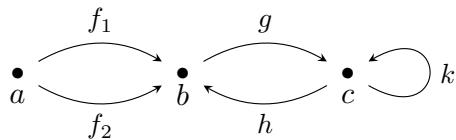
\includegraphics[keepaspectratio]{images/part001_552ae758.jpg}}

represents a quiver whose vertices are a, b, c, and whose arrows are \(f_{1}, f_{2}, g, h, k\) and the source and target maps are given by

\[
\begin{array}{c c c c} o (f _ {1}) = o (f _ {2}) = a & \quad o (g) = b & \quad o (h) = c & \quad o (k) = c \\ t (f _ {1}) = t (f _ {2}) = b & \quad t (g) = c & \quad t (h) = b & \quad t (k) = c. \end{array}
\]

\subsection{Subquivers}

Let C and C′ be quivers. We say that C′ is a subquiver of C if we have \(\operatorname{Som}(\mathrm{C}') \subset \operatorname{Som}(\mathrm{C})\) , \(\operatorname{Fl}(\mathrm{C}') \subset \operatorname{Fl}(\mathrm{C})\) and that the maps \(o_{C'}\) and \(t_{C'}\) coincide with the maps \(o_{C}\) and \(t_{C}\) on \(\operatorname{Fl}(\mathrm{C}')\) . If, moreover, every arrow of C whose source and target belong to \(\operatorname{Som}(\mathrm{C}')\) is an arrow of C', one says that C' is a full subquiver of C.

Let C be a quiver and let \((\mathrm{C}_{i})_{i\in\mathrm{I}}\) be a family of subquivers of C. One calls the intersection of the family \((\mathrm{C}_{i})_{i\in\mathrm{I}}\) and denotes by \(\bigcap_{i\in I}C_{i}\) the subquiver of C whose set of vertices is \(\bigcap_{i\in I}\mathrm{Som}(\mathrm{C}_{i})\) and whose set of arrows is \(\bigcap_{i\in I}\mathrm{Fl}(\mathrm{C}_{i})\) .

\subsection{Morphisms of quivers}

Let C and C' be quivers. A morphism of quivers from C to C' is a pair \((u,v)\) , where \(u\colon\operatorname{Som}(\mathrm{C})\to\operatorname{Som}(\mathrm{C}')\) and \(v\colon\operatorname{Fl}(\mathrm{C})\to\operatorname{Fl}(\mathrm{C}')\) are maps such that \(o_{C'}\circ v=u\circ o_{C}\) and \(t_{C'}\circ v=u\circ t_{C}\) .

Let \(\varphi = (u, v)\) be a morphism of quivers from C to C'. The maps \(u\) and \(v\) are denoted \(\operatorname{Som}(\varphi)\) and \(\operatorname{Fl}(\varphi)\) . If \(a\) is a vertex of C, one will denote, by abuse of notation, \(\varphi(a)\) the image of the vertex \(a\) under \(\varphi\) and we will say that \(\varphi(a)\)

is the image of \(a\) under \(\varphi\) . Similarly, if \(f\) is an arrow of C, we will denote, by abuse of notation, \(\varphi(f)\) the arrow \(v(f)\) of C' and we will say that it is the image of \(f\) under \(\varphi\) .

Let C, \(C'\) , \(C''\) be three quivers, namely \(\varphi = (u, v)\) a morphism from C to \(C'\) and let \(\varphi' = (u', v')\) be a morphism from \(C'\) to \(C''\) . Then \((u' \circ u, v' \circ v)\) is a morphism from C to \(C''\) , denoted \(\varphi' \circ \varphi\) and which is called the composite of \(\varphi'\) and of \(\varphi\) .

We denote \(\mathrm{Id}_{\mathrm{C}}\) the morphism \((\mathrm{Id}_{\mathrm{Som}(\mathrm{C})}, \mathrm{Id}_{\mathrm{Fl}(\mathrm{C})})\) from C into itself.

Let \(\varphi\) be a quiver morphism from C to C'. For \(\varphi\) to be an isomorphism, it is necessary and sufficient that the maps \(\operatorname{Som}(\varphi)\) and \(\operatorname{Fl}(\varphi)\) are bijective (cf. E, IV, p. 6).

Thus, if one calls a quiver structure on sets S and F the data of two maps \(o, t: \mathrm{F} \to \mathrm{S}\) one can take quiver morphisms as morphisms of this structure (E, IV, p. 11).

Let \(\varphi\) be a quiver morphism from C to C'. There exists a unique subquiver of C' whose sets of vertices and arrows are the images of \(\mathrm{Som}(\varphi)\) and \(\mathrm{Fl}(\varphi)\) respectively. It is denoted \(\varphi(\mathrm{C})\) and it is called the image of C under \(\varphi\) . One says that \(\varphi\) is injective if the maps \(\mathrm{Som}(\varphi)\) and \(\mathrm{Fl}(\varphi)\) are injective; in this case, \(\varphi\) induces an isomorphism from C onto its image.

Let \(\varphi\) and \(\psi\) be morphisms of quivers from C to C'. There exists a unique subquiver of C whose vertices and arrows are respectively the vertices and arrows of C having the same image under \(\varphi\) and \(\psi\) . We call it the equalizer of \(\varphi\) and \(\psi\) .

\subsection{Products of quivers}

Let \((\mathrm{C}_{i})_{i\in\mathrm{I}}\) be a family of quivers. Set \(S = \prod_{i\in\mathrm{I}} \mathrm{Som}(\mathrm{C}_{i})\) , \(F = \prod_{i\in\mathrm{I}} \mathrm{Fl}(\mathrm{C}_{i})\) and let o and t be the maps \(\prod_{i\in\mathrm{I}} o_{C_{i}}\) and \(\prod_{i\in\mathrm{I}} t_{C_{i}}\) respectively. The quadruplet \(C = (S, F, o, t)\) is a quiver called the product quiver of the family \((\mathrm{C}_{i})_{i\in\mathrm{I}}\) .

There exists a unique quiver morphism \(pr_{i}: C \to C_{i}\) such that the maps \(\operatorname{Som}(\operatorname{pr}_{i})\) and \(\operatorname{Fl}(\operatorname{pr}_{i})\) are respectively the index-i projections of \(\operatorname{Som}(C)\) onto \(\operatorname{Som}(C_{i})\) and of \(\operatorname{Fl}(C)\) onto \(\operatorname{Fl}(C_{i})\) .

We have the following universal property: Let C' be a quiver; for any family \((\varphi_{i})_{i\in\mathrm{I}}\) where, for every \(i\in I\) , \(\varphi_{i}\colon C'\to C_{i}\) is a quiver morphism, there exists a unique quiver morphism \(\varphi\colon\mathrm{C}^{\prime}\to\mathrm{C}\) such that \(\varphi_{i}=\mathrm{pr}_{i}\circ\varphi\) for all \(i\in\mathrm{I}\) .

\subsection{Paths and loops in a quiver}

DEFINITION 2. --- Let C be a quiver. A path in C is a sequence \(c = (a_{0}, f_{1}, a_{1}, \ldots, a_{n-1}, f_{n}, a_{n})\) , where \(n\) is an integer \(\geqslant 0\) , \(a_{0}, \ldots, a_{n}\) are vertices of C and where, for \(1 \leqslant i \leqslant n\) , \(f_{i}\) is an arrow of C connecting \(a_{i-1}\) to \(a_{i}\) . We say that the path c has length \(n\) .

Let \(c = (a_{0}, f_{1}, a_{1}, \ldots, a_{n-1}, f_{n}, a_{n})\) be a path of length n in C. The vertex \(a_{0}\) is called the origin, or source, of c; the vertex \(a_{n}\) is called the term, or the target, of c; one also says that c joins the vertex \(a_{0}\) to the vertex \(a_{n}\) . The vertex \(a_{i}\) , for \(0 \leqslant i \leqslant n\) , is called the vertex of index i; the arrow \(f_{i}\) , for \(1 \leqslant i \leqslant n\) , is called the i-th arrow, or the arrow of index i. A path of length \(\geqslant 1\) is determined by the sequence of its arrows.

A path whose origin is equal to its endpoint is called a loop. A path of length 0 is a loop, said to be constant.

We say that paths

\[
c = (a _ {0}, f _ {1}, a _ {1}, \ldots , a _ {n - 1}, f _ {n}, a _ {n}) \text{and} c ^ {\prime} = (a _ {0} ^ {\prime}, f _ {1} ^ {\prime}, a _ {1} ^ {\prime}, \ldots , a _ {m - 1} ^ {\prime}, f _ {m} ^ {\prime}, a _ {m} ^ {\prime})
\]

in C are juxtaposable if the endpoint \(a_{n}\) of c is the origin \(a_{0}^{\prime}\) of \(c^{\prime}\) . In this case, the sequence \((a_{0}, f_{1}, a_{1}, \ldots, a_{n-1}, f_{n}, a_{n}, f_{1}^{\prime}, a_{1}^{\prime}, \ldots, f_{m}^{\prime}, a_{m}^{\prime})\) is a path in C, denoted \(c * c^{\prime}\) and called the juxtaposed path of c and \(c^{\prime}\) . It joins the origin of c to the endpoint of \(c^{\prime}\) ; its length is the sum of the lengths of the paths c and \(c^{\prime}\) .

\subsection{Connected components of a quiver}

Let \(C = (S, F, o, t)\) be a quiver. Consider the equivalence relation \(R_{C}\) on S, the finest such that the relation \(\mathrm{R}_{\mathrm{C}}\{o(f), t(f)\}\) is satisfied for every arrow f of C. Two vertices a, b of C are equivalent for this relation if and only if there exists an integer \(n \geqslant 0\) , vertices \(a_{0}, \ldots, a_{n}\) of C and arrows \(f_{1}, \ldots, f_{n}\) of C such that \(a_{0} = a\) , \(a_{n} = b\) and such that, for \(1 \leqslant i \leqslant n\) , the arrow \(f_{i}\) joins either \(a_{i-1}\) to \(a_{i}\) , or \(a_{i}\) to \(a_{i-1}\) .

The equivalence classes of this equivalence relation are called the connected components of C. We denote by \(\pi_0(\mathrm{C})\) the set of connected components of C. Finally, we say that C is connected if it has at most one connected component.

Let \(\varphi\colon\mathrm{C}\to\mathrm{C}^{\prime}\) be a morphism of quivers. The map \(\operatorname{Som}(\varphi)\) defines, by passing to quotients, a map from \(\pi_{0}(\mathrm{C})\) to \(\pi_{0}(\mathrm{C}^{\prime})\) which we denote \(\pi_{0}(\varphi)\) .

\section{GRAPHS}

\subsection{Definition of a graph}

DEFINITION 1. --- A graph \(^{(1)}\) is a quiver (S, F, o, t) equipped with an involution of F, denoted \(f \mapsto \overline{f}\) , without fixed point and such that \(t(\overline{f}) = o(f)\) for all \(f \in F\) .

The quiver (S, F, o, t) is said to be underlying this graph. For every arrow f of this quiver, we have, by definition, \(\overline{\overline{f}} = f\) , \(\overline{f} \neq f\) and \(t(\overline{f}) = o(f)\) . By applying this last relation to the arrow \(\overline{f}\) , one obtains the equality \(o(\overline{f}) = t(f)\) . The arrow \(\overline{f}\) is called the arrow opposite to f.

A pair of opposite arrows of the graph is called an edge of the graph. Each of the two arrows belonging to this pair is called an orientation of this edge. For this reason, the arrows of a graph are also called the oriented edges of the graph.

If G and G' are graphs, a graph morphism from G to G' is a quiver morphism \(\varphi\colon\mathrm{G}\to\mathrm{G}'\) such that \(\overline{\varphi(f)}=\varphi(\overline{f})\) for every arrow \(f\) of G.

Let G and G' be graphs; one says that G' is a subgraph of G if it is a subquiver and if the involution of Fl(G') is the restriction of that of Fl(G).

\subsection{Orientation of a graph}

Let G be a graph. An orientation of G is a subset A of the set of arrows of G such that \(A \cap \overline{A} = \varnothing\) and \(A \cup \overline{A} = \mathrm{Fl}(G)\) .

A graph equipped with an orientation is called an oriented graph.

Let G be an oriented graph and let A be its orientation; an oriented subgraph of G is a subgraph \(G'\) of G equipped with the orientation \(A' = \mathrm{Fl}(G') \cap A\) .

Let (G, A) and (G', A') be oriented graphs. A morphism of oriented graphs from (G, A) to (G', A') is a graph morphism \(\varphi\colon G \to G'\) such that \(\operatorname{Fl}(\varphi)(A) \subset A'\) .

\subsection{Oriented graphs and quivers}

Let G be a graph, \((S,F,o,t)\) the underlying quiver, and A an orientation of G. Then, \((S,A,o\mid A,t\mid A)\) is a quiver, called the quiver associated with the oriented graph \((G,A)\) .

Conversely, let \(C = (S, F, o, t)\) be a quiver. Set \(\widetilde{F} = F \times \{-1, 1\}\) and let \(\widetilde{o}, \widetilde{t}\) be the maps from \(\widetilde{F}\) to S defined by

\[
\begin{array}{l l} \widetilde {o} (f, 1) = o (f) & \qquad \qquad \widetilde {o} (f, - 1) = t (f) \\ \widetilde {t} (f, 1) = t (f) & \qquad \qquad \widetilde {t} (f, - 1) = o (f), \end{array}
\]

for every \(f \in \mathrm{F}\) . Then, \(\widetilde{\mathrm{C}} = (\mathrm{S}, \widetilde{\mathrm{F}}, \widetilde{o}, \widetilde{t})\) , equipped with the involution \((f, \varepsilon) \mapsto (f, -\varepsilon)\) of \(\widetilde{\mathrm{F}}\) is a graph, called the graph associated with the quiver C. The set \(\mathrm{A} = \mathrm{F} \times \{1\}\) is an orientation of this graph. One says that \((\widetilde{\mathrm{C}}, \mathrm{A})\) is the oriented graph associated with the quiver C.

If \(f\) is an arrow of C, one also says that \((f,1)\) is the oriented edge of \(\widetilde{C}\) associated with \(f\) and that the pair \(\{(f,1),(f,-1)\}\) is the edge of \(\widetilde{C}\) associated with \(f\) .

If C' is a subquiver of C, the directed graph \(\widetilde{C}'\) is a directed subgraph of \(\widetilde{C}\) .

There exists a unique quiver morphism \(\varphi\) from C to the quiver underlying \(\widetilde{\mathrm{C}}\) such that \(\varphi(f) = (f,1)\) for every arrow \(f\) of C; it is an isomorphism from C onto the quiver associated with the oriented graph ( \(\widetilde{\mathrm{C}}\) , A).

\subsection{Trees}

When one speaks of paths, or of connected components, of a graph, one means the paths or the connected components of the underlying quiver. Two vertices of a graph belong to the same connected component if and only if there exists a path connecting them.

Let G be a graph. If \(c = (a_{0}, f_{1}, a_{1}, \ldots, f_{n}, a_{n})\) is a path in G, the sequence \(\overline{c} = (a_{n}, \overline{f_{n}}, \ldots, a_{1}, \overline{f_{1}}, a_{0})\) is a path in G, called the opposite path to c. Let c and \(c'\) be juxtaposable paths in G; then, \(\overline{c'}\) and \(\overline{c}\) are juxtaposable, and one has \(\overline{c * c'} = \overline{c'} * \overline{c}\) .

A path c in G is said to be without backtracking if there is no pair of consecutive arrows of c that are opposite. Let \(c = (a_{0}, f_{1}, \ldots, f_{n}, a_{n})\) be a path in G connecting \(a_{0}\) and \(a_{n}\) . If, for an integer i such that \(1 \leqslant i < n\) , the arrows \(f_{i}\) and \(f_{i+1}\) are opposite, the path \((a_{0}, f_{1}, \ldots, a_{i-1}, f_{i+2}, \ldots, f_{n}, a_{n})\) is a path in G connecting \(a_{0}\) to \(a_{n}\) whose length is strictly less than that of the path c. By induction, there therefore exists a path without backtracking in G that connects \(a_{0}\) to \(a_{n}\) .

DEFINITION 2. --- A forest is a graph in which every loop without backtracking is a constant loop. A tree is a connected forest.

PROPOSITION 1. --- Let G be a graph. Every forest of G is contained in a maximal forest of G; in particular, there exists a maximal forest of G.

For a forest of G to be maximal, it is necessary and sufficient that its vertex set be equal to the vertex set of G and that its connected components be those of G.

Let \(A_{0}\) be a forest of G. The set of forests of G, equipped with the order relation “A is a subgraph of B,” is inductive. Consequently, there exists a maximal forest of G of which \(A_{0}\) is a subgraph (E, III, p. 21, cor. 1).

The subgraph of G whose vertex set is \(\operatorname{Som}(G)\) and whose arrow set is empty is a forest of G. Hence there exists a maximal forest of G.

Let A be a maximal forest of G. We prove that A and G have the same vertex set. The subgraph of G whose vertex set is \(\operatorname{Som}(G)\) and whose set of arrows is \(\operatorname{Fl}(A)\) is a forest and A is a subgraph of it. Thus we have \(\operatorname{Som}(A) = \operatorname{Som}(G)\) .

We now prove that A and G have the same connected components. Since every arrow of A is an arrow of G, each connected component of A is contained in a connected component of G. Since A and G have the same vertex set, it suffices to show that two vertices of G lying in the same connected component of G lie in the same connected component of A. If this is not the case, the relation \(R_{A}\) , "being in the same connected component of A," is strictly finer than the relation \(R_{G}\) and there exist two vertices of G that are not in the same connected component of A but are nevertheless joined by an arrow f of G. Let B be the directed subgraph of G whose vertex set is \(\operatorname{Som}(G)\) and whose arrow set is \(\mathrm{Fl(A)} \cup \{f, \overline{f}\}\) . Let us prove that B is a forest of G. Let \(c = (a_{0}, f_{1}, \ldots, f_{n}, a_{n})\) be a nonconstant loop without backtracking in B of minimal length. Since A is a forest, the loop c is not a loop in A. Let i (resp. j) be the smallest (resp. the largest) integer of \(\{0, \ldots, n\}\) such that \(a_{0}\) and \(a_{i}\) (resp. \(a_{j}\) and \(a_{n}\) ) are not in the same connected component of A. This means that the arrows \(f_{i}\) and \(f_{j+1}\) are oriented arrows of B associated with the edge \(\{f, \overline{f}\}\) and that they are opposite. Since the loop c has no back-and-forth, \(f_{i+1} \neq \overline{f_{i}}\) , therefore \(i \neq j\) and the path \((a_{i}, f_{i+1}, a_{i+1}, \ldots, f_{j}, a_{j})\) is a non-constant loop without backtracking in B of length < n, contrary to the hypothesis that c is of minimal length. It follows that B is a forest. This contradicts the hypothesis that A is a maximal forest of G.

Let now A be a forest of G such that \(\mathrm{Som}(\mathrm{A}) = \mathrm{Som}(\mathrm{G})\) and \(\pi_{0}(\mathrm{A}) = \pi_{0}(\mathrm{G})\) . Let us prove that this is a maximal forest of G. It suffices to show that if \(f \notin \mathrm{Fl}(\mathrm{A})\) , the subgraph B of G with vertex set \(\mathrm{Som}(\mathrm{G})\) and arrow set \(\mathrm{Fl}(\mathrm{A}) \cup \{f, \overline{f}\}\) is not a forest. By hypothesis, the points \(o(f)\) and \(t(f)\) lie in the same connected component of A; there therefore exists a path c without backtracking in A joining \(o(f)\) to \(t(f)\) . The path \(c * \overline{f}\) is then a loop without backtracking and non-constant in B, which shows that B is not a forest.

COROLLARY. --- A maximal forest of a connected graph is a maximal tree thereof.

Remark 1. --- In LIE, IV, p. 33, appendix, the notion of a combinatorial graph was defined as a pair (A, S), where S is a set and

A a subset of \(\mathfrak{P}(S)\) consisting of two-element sets; the elements of S are called vertices, those of A edges, and two vertices \(x\) and \(y \in S\) are said to be linked if \(\{x, y\}\) is an edge.

To such a combinatorial graph \(\Gamma = (\mathrm{A},\mathrm{S})\) , one associates a graph G whose vertex set is S and whose arrow set \(\widetilde{\mathrm{A}}\) is the subset of \(\mathrm{S}^2\) formed by the pairs of linked vertices, with the source map and the target map coinciding with the first and second projections of \(\mathrm{S}^2\) in S, and the involution \(f\mapsto \overline{f}\) being given by the restriction to \(\widetilde{\mathrm{A}}\) of the map \((x,y)\mapsto (y,x)\) of \(\mathrm{S}^2\) into itself. The map which to an edge \(\{f,\overline{f}\}\) of G associates the set \(\{o(f),t(f)\}\) is a bijection from the set of edges of G onto that of the edges of the combinatorial graph \(\Gamma\) .

Conversely, every graph such that the source and target of every arrow are distinct, and such that an arrow is determined by its source and target, is of this form.

The reader will verify that the notions of connectedness, tree, or forest for a combinatorial graph coincide with the corresponding notions for the graph associated with it.

\section{GROUPOIDS}

\subsection{Categories}

DEFINITION 1. --- Let C be a quiver. Denote by J the set of pairs \((f,g)\) of arrows of C such that \(t(f)=o(g)\) . A composition law in C is a mapping \(m:J\to\mathrm{Fl}(\mathrm{C})\) such that, for every pair \((f,g)\in\mathrm{J}\) , the origin of the arrow \(m(f,g)\) is that of f and its target that of g.

Let C be a quiver equipped with a composition law \(m\) . Two arrows \(f\) and \(g\) such that \(t(f) = o(g)\) are said to be composable; the arrow \(m(f, g)\) is called their composite, or their product, and is often denoted \(f \cdot g\) , or even \(fg\) .

For every vertex \(a\) of C, the set \(\mathrm{C}_{a,a} = \mathrm{Fl}_{a,a}(\mathrm{C})\) , equipped with the map deduced from \(m\) by passing to subsets, is a magma (A, I, p. 1, def. 1).

A family \((f_{i})_{i\in\mathrm{I}}\) of arrows of C, indexed by a finite nonempty totally ordered set I, is said to be composable if, for every pair \((i,j)\) of consecutive elements of I, the arrows \(f_{i}\) and \(f_{j}\) are composable. One defines the product \(\prod_{i\in\mathrm{I}}f_{i}\) of such a family by induction on the cardinality of I as follows (cf. A, I, p. 3):

\begin{enumerate}
\def\labelenumi{(\roman{enumi})}
\item
  if I has a single element \(\omega\) , \(\prod_{i\in I}f_i = f_\omega\) ;
\item
  if I has at least two elements and if \(\omega\) is the smallest element of I, we set \(\prod_{i\in I}f_i = f_\omega \cdot \prod_{i\in I - \{\omega \}}f_i\) .
\end{enumerate}

The composition law \(m\) is said to be associative if one has \(f \cdot (g \cdot h) = (f \cdot g) \cdot h\) for every composable triple \((f, g, h)\) of arrows of C. When the law \(m\) is associative, the product of a sequence \((f_1, \ldots, f_n)\) of \(n\) composable arrows, where \(n\) is an integer \(\geqslant 1\) , is denoted \(f_1 f_2 \ldots f_n\) .

Let \(a\) be a vertex of C. We say that an arrow \(e \in \mathrm{C}_{a,a}\) is an identity element of \(m\) at \(a\) if one has \(ef = f\) for every arrow \(f\) with source \(a\) and \(ge = g\) for every arrow \(g\) with term \(a\) . There exists at most one identity element of \(m\) at \(a\) : if \(e\) and \(e'\) are two of them, one has \(e' = ee' = e\) . When such an identity element exists, it is often denoted \(e_a\) ; it is then an identity element of the magma \(\mathrm{C}_{a,a}\) (A, I, p. 12).

DEFINITION 2. --- A category is a quiver equipped with an associative composition law for which there exists an identity element at each vertex.

Examples. --- 1) Let C be a quiver. Denote by Ch(C) the set of paths in C and by o: Ch(C) → Som(C), t: Ch(C) → Som(C) the maps which, to a path, associate its origin and its terminus. The quadruple \(\Omega_{\mathrm{C}} = (\mathrm{Som}(\mathrm{C}), \mathrm{Ch}(\mathrm{C}), o, t)\) is a quiver. Equip it with the composition law defined by concatenation of paths. This composition law is associative; for every vertex a of C, the constant loop \(e_a = (a)\) with origin a is an identity element at a. Thus, \(\Omega_{\mathrm{C}}\) is a category. It is said to be the category of paths of the quiver C.

\begin{enumerate}
\def\labelenumi{\arabic{enumi})}
\setcounter{enumi}{1}
\tightlist
\item
  Let \(\Sigma\) be a kind of structure in a theory \(\mathcal{T}\) stronger than set theory and let \(\sigma\{x,y,s,u\}\) be a term of \(\mathcal{T}\) satisfying conditions (MO \(_{\text{I}}\) ), (MO \(_{\text{II}}\) ) and (MO \(_{\text{III}}\) ) of E, IV, p. 11. Let S be a set; suppose that every element of S is a pair \((x,s)\), where \(x\) is a set and \(s\) is a structure of species \(\Sigma\) on \(x\) . Let F be the set of mappings \(f\) such that there exist \((x,s)\) and \((y,t)\) in S such that \(f\) is a \(\sigma\) -morphism from \(x\) , equipped with the structure \(s\) , to \(y\) , equipped with the structure \(t\) ; one then sets \(o(f) = (x,s)\) and \(t(f) = (y,t)\) . Endowed with the composition law given by \(m(f,g)=g\circ f\) , the quiver (S,F,o,t) is a category. In this context, the elements of S are rather called objects.
\end{enumerate}

Let C be a category.

For every vertex \(a\) of C, the set \(\mathrm{C}_{a,a}\) , equipped with the composition law \((f,g)\mapsto fg\) , is a monoid with identity element \(e_a\) .

We say that an arrow \(f\) of C is invertible if there exists an arrow \(g\) of C such that \(o(g) = t(f)\) , \(t(g) = o(f)\) and such that \(fg\) and \(gf\) are identity elements at \(o(f)\) and \(t(f)\) respectively. Such an arrow \(g\) is unique (if \(fg = e_{o(f)}\) and \(g'f = e_{t(f)}\) , we have \(g = e_{t(f)}g = (g'f)g = g'(fg) = g'e_{o(f)} = g'\) ) and is called the inverse of \(f\) ; the inverse of an invertible arrow \(f\) is denoted \(f^{-1}\) .

\subsection{Functors}

DEFINITION 3. --- Let C and C' be categories. A functor from C to C' is called a morphism of quivers \(\varphi\colon\mathrm{C}\to\mathrm{C}'\) such that \(\varphi(fg)=\varphi(f)\varphi(g)\) for every pair \((f,g)\) of composable arrows of C.

Let C and C' be categories and let \(\varphi\colon\mathrm{C}\to\mathrm{C}'\) be a functor. Let \(f\) be an arrow of C, \(a\) its origin and \(b\) its target; then, \(\varphi(f)\) is an arrow of C' with origin \(\varphi(a)\) and target \(\varphi(b)\) .

Let C, C', C'' be categories and let \(\varphi\colon\mathrm{C}\to\mathrm{C}'\) and \(\varphi'\colon\mathrm{C}'\to\mathrm{C}''\) be functors. Then, \(\varphi'\circ\varphi\) is a functor.

Let C be a category. Then the morphism of quivers \(Id_{C}\) is a functor.

Let \(\varphi\colon\mathrm{C}\to\mathrm{C}^{\prime}\) be a functor. In order for \(\varphi\) to be an isomorphism, it is necessary and sufficient that the maps \(\operatorname{Som}(\varphi)\) and \(\operatorname{Fl}(\varphi)\) be bijective.

Thus, if one calls a category structure on sets S and F the data of a quiver structure on these sets and of an associative composition law for which there exists at each vertex an identity element, one can take functors as morphisms of the category structure (E, IV, p. 11).

\subsection{Groupoids}

DEFINITION 4. --- A groupoid is a category in which every arrow is invertible.

Let G be a groupoid and let a be a vertex of G. The monoid \(G_{a,a}\) is a group, which we denote by \(G_{a}\) and which we call the isotropy group of G at a.

Let \(a\) and \(b\) be vertices of G and let \(f \in \mathrm{G}_{a,b}\) be an arrow connecting \(a\) to \(b\) . The map \(g \mapsto fgf^{-1}\) is a group isomorphism from \(\mathrm{G}_b\) to \(\mathrm{G}_a\) , denoted \(\operatorname{Int}(f)\) . If \(f\) and \(f'\) are composable arrows of G, we have \(\operatorname{Int}(ff') = \operatorname{Int}(f) \circ \operatorname{Int}(f')\) . The inverse of the isomorphism \(\operatorname{Int}(f)\) is the isomorphism \(\operatorname{Int}(f^{-1})\) .

A morphism of groupoids \(\varphi\colon G\to G'\) is a morphism of categories. Moreover, \(\varphi\) is a groupoid isomorphism if and only if it is a category isomorphism.

Let \(\varphi\colon\mathrm{G}\to\mathrm{G}^{\prime}\) be a groupoid morphism. For every vertex \(a\) of G, the map \(f\mapsto\varphi(f)\) from \(\mathrm{G}_{a}\) to \((\mathrm{G}^{\prime})_{\varphi(a)}\) is a group homomorphism, denoted \(\varphi_{a}\) . In particular, we have \(\varphi(e_{a})=e_{\varphi(a)}\) .

For every arrow \(f\) of G, \(\varphi(f^{-1})\) is the inverse of \(\varphi(f)\) . If \(f\) is an arrow of G connecting a vertex \(a\) to a vertex \(b\) we thus have, for every element \(g \in \mathrm{G}_b\) , the relation \(\operatorname{Int}(\varphi(f))(\varphi(g)) = \varphi(\operatorname{Int}(f)(g))\) .

\subsection{Orbits of a groupoid}

Let G be a groupoid. The connected components of the underlying quiver of G are called the orbits of G. The set of orbits of G is denoted \(\mathrm{Orb}(\mathrm{G})\) ; if \(\varphi: G \to G'\) is a morphism of groupoids, the map \(\pi_{0}(\varphi)\) deduced from \(\varphi\) by passing to the connected components of the associated graphs is generally denoted \(\mathrm{Orb}(\varphi)\) and is called the map deduced from \(\varphi\) by passing to orbits.

A groupoid with exactly one orbit is said to be transitive. If G is a transitive groupoid, the groups \(G_{a}\) , for \(a \in \text{Som}(G)\) , are isomorphic. We say that the groupoid G is simply transitive if it is transitive and if, moreover, the isotropy groups \(G_{a}\) are all reduced to their identity element.

PROPOSITION 1. --- Let G be a groupoid. The relation "there exists an arrow of G connecting a to b" is an equivalence relation on the set of vertices of G, whose equivalence classes are the orbits of G.

Let \(a\) , \(b\) , \(c\) be vertices of G. We have \(e_a \in \mathrm{G}_{a,a}\) ; if \(f \in \mathrm{G}_{a,b}\) , \(f^{-1} \in \mathrm{G}_{b,a}\) ; if \(f \in \mathrm{G}_{a,b}\) and \(g \in \mathrm{G}_{b,c}\) , we have \(fg \in \mathrm{G}_{a,c}\) . This shows that the indicated relation is reflexive, symmetric, and transitive; it is therefore an equivalence relation. The second assertion then follows from the definition of the connected components of a quiver.

\subsection{Examples of groupoids}

\begin{enumerate}
\def\labelenumi{\arabic{enumi})}
\item
  Let G be a group. Denote by \(\mathcal{G}\) the quiver whose set of vertices is reduced to a single element and whose set of arrows is G. Equipped with the composition law induced by that of G, \(\mathcal{G}\) is a groupoid, called the groupoid associated with the group G.
\item
  Let X be a set. Let G be the quiver \((\mathrm{X}, \mathrm{X} \times \mathrm{X}, \mathrm{pr}_{1}, \mathrm{pr}_{2})\) ; define a composition law on G by setting \((x, x') \cdot (x', x'') = (x, x'')\) , if \(x, x', x''\) are elements of X. This law is associative; for every \(x \in X\) , \((x, x)\) is the neutral element at x; the inverse of the arrow \((x, x')\) is the arrow \((x', x)\) . The groupoid thus defined is called the groupoid of pairs of the set X. If X is nonempty, it is simply transitive.
\item
  Let X and S be sets and let \(p \colon \mathrm{X} \to \mathrm{S}\) be a map. For \(a \in \mathrm{S}\) , write \(\mathrm{X}_a = p^{-1}(a)\) . For \(a\) and \(b\) in S, let \(\mathrm{G}_{a,b}\) be the set \(\mathcal{B}(\mathrm{X}_a; \mathrm{X}_b)\) of bijections from \(\mathrm{X}_a\) to \(\mathrm{X}_b\) and let G be the disjoint union of the sets \(\mathrm{G}_{a,b}\) . Let \(o\) and \(t\) be the maps from G to S such that \(o(f) = a\) and \(t(f) = b\) for every element \(f \in \mathrm{G}_{a,b}\) . The quadruple \((\mathrm{S}, \mathrm{G}, o, t)\) is a quiver. Equip it with the composition law defined by \(m(f, g) = g \circ f\) if \(f \in \mathcal{B}(\mathrm{X}_a; \mathrm{X}_b)\) and \(g \in \mathcal{B}(\mathrm{X}_b; \mathrm{X}_c)\) , where \(a, b, c\) are elements of S. This is a groupoid; it is denoted by \(\mathcal{B}(\mathrm{X}, p)\) and it is called the groupoid of permutations of X relative to \(p\) .
\item
  Let \((\mathrm{G}_{i})_{i\in\mathrm{I}}\) be a family of groupoids. Let G denote the product quiver of the family of underlying quivers; for every \(i\in I\) , let \(pr_{i}\colon G\to G_{i}\) be the canonical quiver morphism. There exists a unique composition law in G for which G is a groupoid and such that, for every \(i \in I\) , \(\mathrm{pr}_i\) is a morphism of groupoids. Let \(f = (f_i)_{i \in I}\) and \(g = (g_i)_{i \in I}\) be arrows of G; they are composable if and only if the arrows \(f_i\) and \(g_i\) are composable, for \(i \in I\) . One then has \(fg = (f_i g_i)_{i \in I}\) .
\end{enumerate}

The quiver G, equipped with this composition law, is called the product groupoid of the family \((\mathrm{G}_{i})_{i\in\mathrm{I}}\) . It satisfies the following universal property: for every groupoid \(G'\) and every family \((\varphi_{i})_{i\in\mathrm{I}}\) , where \(\varphi_{i}\) is a morphism of groupoids from \(G'\) to \(G_{i}\) , there exists a unique morphism of groupoids \(\varphi: G'\to G\) such that \(\varphi_{i}=\operatorname{pr}_{i}\circ\varphi\) for all \(i\in I\) .

\begin{enumerate}
\def\labelenumi{\arabic{enumi})}
\setcounter{enumi}{4}
\tightlist
\item
  Let \(((\mathrm{G}_{i})_{i\in\mathrm{I}},(\varphi_{i,j})_{i\prec j})\) be an inductive system of groupoids, indexed by a right-filtering preordered set \((\mathrm{I},\prec)\) , the \(\varphi_{i,j}\) being morphisms of groupoids. Let G be the quiver whose set of vertices is \(\varinjlim_{i}\operatorname{Som}(\mathbf{G}_{i})\) and whose set of arrows is \(\varinjlim_{i}\operatorname{Fl}(\mathbf{G}_{i})\) , the source and target maps being the maps \(\varinjlim_{i}o_{G_{i}}\) and \(\varinjlim_{i}t_{G_{i}}\) respectively. The composition laws of the \(G_{i}\) induce a composition law on G which makes it a groupoid (cf. A, I, p. 114). The canonical maps \(\operatorname{Som}(\mathbf{G}_{i})\to\operatorname{Som}(\mathbf{G})\) and \(\operatorname{Fl}(\mathbf{G}_{i})\to\operatorname{Fl}(\mathbf{G})\) define a morphism of groupoids \(\varphi_{i}\) from \(G_{i}\) to G. If i, j are elements of I such that \(i\prec j\) , we have \(\varphi_{j}\circ\varphi_{i,j}=\varphi_{i}\) . The groupoid G is called the inductive limit of the family of groupoids \(G_{i}\) and is denoted \(\varinjlim_{i}G_{i}\) . It satisfies the following universal property: for every groupoid H and every family \((\psi_{i})_{i\in\mathrm{I}}\) , where, for \(i\in I\) , \(\psi_{i}:G_{i}\to H\) is a morphism of groupoids, such that \(\psi_{j}\circ\varphi_{i,j}=\psi_{i}\) for every pair \((i,j)\) of elements of I such that \(i\prec j\) , there exists a unique morphism of groupoids \(\psi:G\to H\) such that \(\psi_{i}=\psi\circ\varphi_{i}\) .
\end{enumerate}

For the existence of a groupoid satisfying this universal property when one does not assume that the set I is filtering to the right, cf. II, p. 228, exerc. 3.
% semantic-fragments: legacy-input-seam
\relax{}
\subsection{Subgroupoids}

DEFINITION 5. --- Let C be a category. A subcategory of C is a subquiver D of C satisfying the following conditions:

\begin{enumerate}
\def\labelenumi{(\roman{enumi})}
\item
  For every vertex a of D, \(e_a\) is an arrow of D;
\item
  For every composable pair \((f,g)\) of arrows of C belonging to D, the product fg is an arrow of D;
\end{enumerate}

Let C be a category and let D be a subcategory of C; endowed with the composition law induced from that of C by restriction to subsets, D is a category.

Every full subquiver of C is a subcategory of C. The intersection of a family of subcategories of C is a subcategory of C.

DEFINITION 6. --- Let G be a groupoid. A subgroupoid of G is a subcategory H of G such that the inverse of every arrow of G belonging to H is an arrow of H.

Let G be a groupoid. Every subgroupoid of G is a groupoid. Every full subquiver of G is a subgroupoid of G. The intersection of a family of subgroupoids of G is a subgroupoid of G.

Let H be a subquiver of G. The intersection of the subgroupoids of G of which H is a subquiver is called the subgroupoid of G generated by H. The set of its vertices is equal to that of H and its orbits are the connected components of H.

Examples. --- 1) Let X be a set; denote by X × X the groupoid of pairs of X (II, p. 163, example 2). Let R be an equivalence relation on X. The subquiver of the groupoid X × X whose set of vertices is X and whose set of arrows is the graph of the equivalence relation R is a subgroupoid of X × X. Its orbits are the equivalence classes of the relation R.

Conversely, every subgroupoid of X × X whose set of vertices is X is of this form.

Let X and S be sets and let \(p: X \rightarrow S\) be a map. The map p defines an equivalence relation on X (E, II, p. 41). We denote by \(X \times_{S} X\) the subgroupoid of \(X \times X\) defined by this equivalence relation and call it the groupoid of pairs of \((X, p)\) .

\begin{enumerate}
\def\labelenumi{\arabic{enumi})}
\setcounter{enumi}{1}
\item
  Let G and G' be groupoids, and let \(\varphi\) and \(\psi\) be morphisms of groupoids from G to G'. The equalizer of \(\varphi\) and \(\psi\) (cf. II, p. 153) is a subgroupoid of G.
\item
  Let X be a set and \(\Gamma\) a group. Denote by \(X \times \Gamma \times X\) the quiver whose set of vertices is X, whose set of arrows is \(X \times \Gamma \times X\) , the source and target maps being respectively \(\mathrm{pr}_1\) and \(\mathrm{pr}_3\) . Endowed with the composition law \((x, \gamma, x') \cdot (x', \gamma', x'') = (x, \gamma \gamma', x'')\) , this is a groupoid. It is moreover the groupoid deduced by transport of structure from the groupoid \((\mathrm{X}\times\mathrm{X})\times\Gamma\) , the product of the groupoid of pairs \(X\times X\) and the groupoid associated with the group \(\Gamma\) (II, p. 163, example 1), by means of the bijection \((x,x',\gamma)\mapsto(x,\gamma,x')\) from \(X\times X\times\Gamma\) to \(X\times\Gamma\times X\) .
\end{enumerate}

Let \(m\colon X \times \Gamma \to X\) be an operation (on the right) of the group \(\Gamma\) on \(X\) . The graph \(F\) of the map \(m\) , that is, the set of triples \((x, \gamma, x') \in X \times \Gamma \times X\) such that \(x' = x\gamma\) , is the set of arrows of a unique subgroupoid \(G\) of \(X \times \Gamma \times X\) . The orbits of this groupoid are the orbits of \(\Gamma\) on \(X\) ; if \(x \in X\) , the isotropy group of \(G\) at \(x\) is the set of \((x, \gamma, x)\) , where \(\gamma\) ranges over the stabilizer of \(x\) in \(\Gamma\) .

Conversely, any subgroupoid G of the groupoid \(X \times \Gamma \times X\) such that the map \((\mathrm{pr}_{1}, \mathrm{pr}_{2})\) from \(\mathrm{Fl}(\mathrm{G})\) to \(X \times \Gamma\) is a bijection is of this form.

\begin{enumerate}
\def\labelenumi{\arabic{enumi})}
\setcounter{enumi}{3}
\tightlist
\item
  Let G be a groupoid, let X be a set, and let \(\varphi\colon\mathrm{X}\to\mathrm{Som}(\mathrm{G})\) be a map. We define a quiver \(\mathrm{G}'\) as follows. The set \(\mathrm{Som}(\mathrm{G}')\) is the set X; for every pair \((x,y)\) of elements of X, the set \(\mathrm{Fl}_{x,y}(\mathrm{G}')\) is the set of triples \((x,f,y)\in\mathrm{X}\times\mathrm{Fl}(\mathrm{G})\times\mathrm{X}\) , where \(f\) is an element of \(\mathrm{Fl}_{\varphi(x),\varphi(y)}(\mathrm{G})\) . Let \(x,y,z\) be elements of X, \(f\in\mathrm{Fl}_{\varphi(x),\varphi(y)}(\mathrm{G})\) and \(g\in\mathrm{Fl}_{\varphi(y),\varphi(z)}(\mathrm{G})\) be arrows of G, and set \((x,f,y)\cdot(y,g,z)=(x,fg,z)\) . This defines a composition law in the quiver \(\mathrm{G}'\), making it a groupoid. It is called the inverse image groupoid of the groupoid G by the map \(\varphi\) and we denote it \(\varphi^{*}(\mathrm{G})\) .
\end{enumerate}

The pair \((\varphi,\psi)\) , where \(\psi\colon\mathrm{Fl}(\varphi^{*}(\mathrm{G}))\to\mathrm{Fl}(\mathrm{G})\) is the map defined by \((x,f,y)\mapsto f\) , is a morphism of groupoids from \(\varphi^{*}(\mathrm{G})\) to G, called the canonical morphism.

\begin{enumerate}
\def\labelenumi{\arabic{enumi})}
\setcounter{enumi}{4}
\tightlist
\item
  Let \(\varphi\colon\mathrm{G}\to\mathrm{G}^{\prime}\) be a morphism of groupoids. Let H be the subquiver of G with vertex set \(\mathrm{Som}(\mathrm{G})\) and whose set of arrows consists of the \(f\in\mathrm{Fl}(\mathrm{G})\) such that \(\varphi(f)\) is an identity element of \(\mathrm{G}^{\prime}\) . For all \(a\in\mathrm{Som}(\mathrm{G})\) , \(e_{a}\in\mathrm{H}_{a,a}\) . For all \(f\in\mathrm{Fl}(\mathrm{H})\) , \(\varphi(f^{-1})=\varphi(f)^{-1}\) ; therefore \(f^{-1}\in\mathrm{Fl}(\mathrm{H})\) . Moreover, if \(f\) and \(g\) are composable arrows of H, then \(\varphi(fg)=\varphi(f)\varphi(g)=e_{t(\varphi(f))}e_{o(\varphi(g))}=e_{t(\varphi(f))}\) , therefore \(fg\) is an arrow of H. This proves that H is a subgroupoid of G. It is called the kernel of \(\varphi\) and we denote it \(\mathrm{Ker}(\varphi)\) .
\end{enumerate}

\pandocbounded{
\includegraphics[keepaspectratio]{images/part002_cf856079.jpg}}

\begin{enumerate}
\def\labelenumi{\arabic{enumi})}
\setcounter{enumi}{5}
\tightlist
\item
  Let \(\varphi\colon\mathrm{G}\to\mathrm{G}^{\prime}\) be a morphism of groupoids. The quiver \(\varphi(\mathrm{G})\) whose set of vertices is \(\varphi(\mathrm{Som}(\mathrm{G}))\) and whose set of arrows is \(\varphi(\mathrm{Fl}(\mathrm{G}))\) is in general not a subgroupoid of \(\mathrm{G}^{\prime}\) .
\end{enumerate}

This is nevertheless the case if the map Som( \(\varphi\) ) is injective (II, p. 225, exerc. 5).

\subsection{Operations of a groupoid}

Let G be a groupoid; denote by S the set of its vertices. Let X be a set and let \(p\colon \mathrm{X}\to \mathrm{S}\) be a map. A (right) operation \(\varphi\) of the groupoid G on the set X, relative to \(p\) , is a morphism of groupoids \(\varphi\) from G to the groupoid \(\mathcal{B}(\mathrm{X},p)\) of the permutations of the set X relative to \(p\) (II, p. 163) which induces the identity on the set of vertices. In other words, \(\varphi\) is the data, for every pair \((a,b)\) of points of S and for every arrow \(g\in \mathrm{G}\) joining \(a\) to \(b\), of a map \(\varphi (g)\colon \mathrm{X}_a\to \mathrm{X}_b\) , such that for every pair \((f,g)\) of composable arrows of G,

\[
\varphi (f g) = \varphi (g) \circ \varphi (f),
\]

and such that, for every \(a \in S\) , \(\varphi(e_a)\) is the identity of \(X_a\) .

Let \(\varphi\) and \(\varphi'\) be operations of the groupoid G on a set X, relative to a map \(p\colon X\to S\) . For \(\varphi=\varphi'\) , it suffices that there exist a subquiver H of G, generating G, such that \(\varphi(f)=\varphi'(f)\) for all \(f\in\mathrm{Fl}(\mathrm{H})\) . Indeed, the set of arrows \(f\) of G such that \(\varphi(f)=\varphi'(f)\) is the set of arrows of a subgroupoid of G, with vertex set S.

Let G be a groupoid with vertex set S, let X be a set, let \(p \colon \mathrm{X} \to \mathrm{S}\) be a map and let \(\varphi\) be an operation of G on X relative to \(p\) . Let \(\mathrm{G}_{\varphi}\) be the subquiver of \(p^{*}(\mathrm{G})\) whose set of vertices is X and whose set of arrows is the set of triples \((x, f, y) \in \mathrm{X} \times \mathrm{Fl}(\mathrm{G}) \times \mathrm{X}\) such that \(\varphi(f)(x) = y\) . It is a subgroupoid of \(p^{*}(\mathrm{G})\) .

Conversely, let \(\Gamma\) be a subgroupoid of \(p^{*}(\mathrm{G})\) ; suppose that the map \((x,f,y)\mapsto (x,f)\) from \(\mathrm{Fl}(\Gamma)\) to \(\mathrm{X}\times \mathrm{Fl}(\mathrm{G})\) is injective and that its image is the set of pairs \((x,f)\) such that \(p(x) = o(f)\) . There then exists a unique operation \(\varphi\) of the groupoid G on X such that one has \(\Gamma = \mathrm{G}_{\varphi}\) .

The orbits of the groupoid \(G_{\varphi}\) are called the orbits of the operation of G on X. By definition, they are the equivalence classes of the relation on X given by \(R\{x,y\}\) if and only if there exists \(f \in \mathrm{Fl}(G)\) such that \(\varphi(f)(x) = y\) .

Examples. --- 1) Let G be a group, let \(\mathcal{G}\) be the groupoid associated with G (II, p. 163, example 1). If X is a set, a (right) action of the groupoid \(\mathcal{G}\) on X is none other than a (right) action of the group G on X. Moreover, the orbits of the action of \(\mathcal{G}\) coincide with those of the group G.

\begin{enumerate}
\def\labelenumi{\arabic{enumi})}
\setcounter{enumi}{1}
\tightlist
\item
  Let \(\mathrm{G} = (\mathrm{S},\mathrm{F},o,t)\) be a groupoid. There exists a unique operation of \(\mathrm{G}\) on the set \(\mathrm{S}\) , relative to \(\mathrm{Id}_{\mathrm{S}}\) . It is given by \(\varphi(f)(a) = b\) if \(f \in \mathrm{G}_{a,b}\) . The orbits for this operation are the orbits of \(\mathrm{G}\) in the sense defined on p. 162.
\end{enumerate}

Let G be a groupoid, let S be the set of its vertices, let X be a set and let \(p: X \to S\) be a map. Let \(\varphi\) be an operation of G on X relative to p. One says that the groupoid G operates without monodromy on X if, for every point \(a \in S\) and every element \(f \in G_{a}\) , \(\varphi(f)\) is the identity of \(X_{a}\) . If the groupoid G is transitive, it suffices that this be so for one point of S.

Let \(a\) be a point of S and suppose that one has \(\varphi(f) = \mathrm{Id}_{\mathrm{X}_a}\) for all \(f \in \mathrm{G}_a\) . Let \(b\) be a point of S belonging to the orbit of \(a\) and let \(g\) be an arrow of G connecting \(a\) to \(b\) . For all \(f \in \mathrm{G}_b\) , \(\mathrm{Int}(g)(f) = gfg^{-1}\) is an element of \(\mathrm{G}_a\) ; one therefore has \(\mathrm{Id}_{\mathrm{X}_a} = \varphi(gfg^{-1}) = \varphi(g)\varphi(f)\varphi(g)^{-1}\) , so that \(\varphi(f) = \mathrm{Id}_{\mathrm{X}_b}\) . Let \(b\) be a point of S belonging to the orbit of \(a\) and let \(g\) , \(g'\) be arrows of G connecting \(a\) to \(b\) ; then \(g'g^{-1}\) is a loop at \(a\) , whence \(\varphi(g'g^{-1}) = \mathrm{Id}_{\mathrm{X}_a}\) and \(\varphi(g) = \varphi(g')\) .

\subsection{Distinguished subgroupoids; quotients of groupoids}

DEFINITION 7. --- Let G be a groupoid. One says that a subgroupoid H of G is distinguished if Som(H) = Som(G) and if, for every pair (a, b) of vertices of H and every arrow \(f \in \mathrm{G}_{a,b}\) , one has \(Int(f)(H_b) = H_a\) .

Let G be a groupoid and let H be a subgroupoid of G whose set of vertices is equal to Som(G). To verify that H is distinguished, it suffices to show that \(fH_{b}f^{-1} \subset H_{a}\) for all \(a \in \text{Som}(G)\) , all \(b \in \text{Som}(\mathbf{G})\) and every \(f \in \mathbf{G}_{a,b}\) . Indeed, if this is so, we also have \(f^{-1}\mathrm{H}_a f \subset \mathrm{H}_b\) for every arrow \(f \in \mathbf{G}_{b,a}\) , that is, \(\mathrm{H}_a \subset f\mathrm{H}_b f^{-1}\) , and, consequently, \(f\mathrm{H}_b f^{-1} = \mathrm{H}_a\) .

Let G be a groupoid and let H be a distinguished subgroupoid of G. For every vertex a of G, the subgroup \(H_{a}\) of \(G_{a}\) is a distinguished subgroup of \(G_{a}\) .

Let \(\varphi\colon\mathrm{G}\to\mathrm{G}^{\prime}\) be a morphism of groupoids. The kernel of \(\varphi\) (II, p. 166, example 5) is a distinguished subgroupoid of G. Indeed, let \(f\) be an arrow in G connecting \(a\) to \(b\) and let \(g\in\mathrm{Ker}(\varphi)_{b}\) ; we then have \(\varphi(fgf^{-1})=\varphi(f)\varphi(g)\varphi(f^{-1})=\varphi(f)e_{\varphi(b)}\varphi(f)^{-1}=e_{\varphi(a)}\) , whence the inclusion \(f\mathrm{Ker}(\varphi)_{b}f^{-1}\subset\mathrm{Ker}(\varphi)_{a}\) .

Let G be a groupoid. The groupoid G and the subgroupoid of G whose set of arrows is the set of identity elements of G are distinguished subgroupoids of G. The intersection of a family of distinguished subgroupoids of G is a distinguished subgroupoid of G. In particular, for every subset F ⊂ Fl(G), there exists a smallest distinguished subgroupoid of G whose set of arrows contains F. It is called the distinguished subgroupoid generated by F.

Let H be a distinguished subgroupoid of G. Let R be the equivalence relation in \(\mathrm{Fl}(\mathrm{G})\) defined by \(R\{f,g\}\) if and only if there exist arrows x and y in \(\mathrm{Fl}(\mathrm{H})\) such that f = xgy. If f and g are arrows of G equivalent modulo R, their origins (resp. their targets) belong to the same orbit of H. Set \(F' = \mathrm{Fl}(\mathrm{G}) / \mathcal{R}\) and denote by \(o'\) and \(t'\) the maps from \(F'\) to \(\mathrm{Orb}(\mathrm{H})\) deduced from o and t by passing to quotients. Denote by G/H the quiver \((\mathrm{Orb}(\mathrm{H}), \mathrm{F}', o', t')\) .

Lemma. --- Given composable arrows u and v of G/H, one can choose representatives f and g of u and v in Fl(G) which are composable. The class modulo R of the product fg does not depend on the choice of f and g.

Let \(f\) and \(g\) be arbitrary representatives of \(u\) and \(v\) in \(\mathrm{Fl(G)}\) . The target of \(f\) and the origin of \(g\) belong to the same orbit of H, hence can be connected by an arrow \(x\) of H (II, p. 162, prop. 1). The arrows \(fx\) and \(g\) are then representatives of \(u\) and \(v\) in F that are composable in G. This proves the first assertion.

Now let \(f\) , \(g\) on the one hand, and \(f'\) , \(g'\) on the other hand, be representatives of \(u\) and \(v\) which are composable in G. By hypothesis, there exist arrows \(x\) , \(y\) , \(z\) , \(t\) in H such that one has \(f' = xfy\) and \(g' = zgt\) . One then has \(yz \in \mathrm{H}_{t(f)}\) and \(f'g' = x f y z g t = x f(yz)f^{-1}f g t\) . Since H is a distinguished subgroupoid of G, the arrow \(f(yz)f^{-1}\) is an arrow of H. The same is therefore true of the arrow \(x f(yz)f^{-1}\) , which proves that \(f'g'\) and \(fg\) are equivalent modulo \(\mathcal{R}\) .

By virtue of this lemma, there exists a unique composition law \(m\) in the quiver G/H such that, for every pair \((u,v)\) of composable arrows, \(m(u,v)\) is the class modulo \(\mathcal{R}\) of the product \(fg\) , for every pair \((f,g)\) of composable arrows of G such that \(u\) is the class of \(f\) and \(v\) that of \(g\) . Endowed with this composition law, G/H is a groupoid. Let \(p_1\colon \operatorname{Som}(\mathrm{G}) \to \operatorname{Som}(\mathrm{G}/\mathrm{H})\) and \(p_2\colon \operatorname{Fl}(\mathrm{G}) \to \operatorname{Fl}(\mathrm{G}/\mathrm{H})\) be the canonical surjections. The pair \(p = (p_1,p_2)\) is a groupoid morphism from G to G/H whose kernel is the distinguished subgroupoid H.

DEFINITION 8. --- We say that G/H is the quotient groupoid of G by H and that p: G → G/H is the canonical morphism.

Remarks. --- 1) The map Som(p) defines, by passing to quotients, a bijection from the set of orbits of G to the set of orbits of G/H. In particular, G is transitive if and only if G/H is.

\begin{enumerate}
\def\labelenumi{\arabic{enumi})}
\setcounter{enumi}{1}
\tightlist
\item
  Let \(a\) and \(b\) be vertices of G. The map from \(\mathrm{G}_{a,b}\) to \((\mathrm{G} / \mathrm{H})_{p(a),p(b)}\) deduced from \(p\) is surjective. Indeed, let \(u\) be an arrow from G/H connecting \(p(a)\) to \(p(b)\) ; it is the class modulo \(\mathcal{R}\) of an arrow \(f\) of G. The origin \(o(f)\) of \(f\) belongs to the orbit of \(a\) in H; there therefore exists an arrow \(x\) in H connecting \(a\) to \(o(f)\) . Similarly, there exists an arrow \(y\) in H that connects \(t(f)\) to \(b\) . Then, \(f' = xfy\) is an element of \(\mathrm{G}_{a,b}\) whose class modulo \(\mathcal{R}\) is \(u\) .
\end{enumerate}

PROPOSITION 2. --- Let a be a vertex of G. The group homomorphism \(p_{a}\colon\mathrm{G}_{a}\to(\mathrm{G}/\mathrm{H})_{p(a)}\) deduced from p by passing to isotropy groups is surjective; its kernel is \(\mathrm{H}_{a}\) .

The homomorphism \(p_a\) is surjective by virtue of the preceding remark. Its kernel contains \(\mathrm{H}_a\) by construction of the groupoid \(\mathrm{G / H}\) . Let \(f\) be an element of \(\mathrm{G}_a\) such that \(p_a(f) = e_{p(a)}\) . This means that \(f\) and \(e_a\) are equivalent modulo \(\mathcal{R}\) ; there then exist arrows \(x\) and \(y\) of H such that \(f = xe_a y\) . Necessarily, \(x\) and \(y\) belong to \(\mathrm{H}_a\) , whence \(f \in \mathrm{H}_a\) .

PROPOSITION 3. --- Let G be a groupoid, let H be a distinguished subgroupoid of G, and let p: G → G/H be the canonical morphism. Let \(\varphi\colon G\to G'\) be a morphism of groupoids such that \(H\subset\operatorname{Ker}(\varphi)\) . There exists a unique groupoid morphism \(\overline{\varphi}\colon G/H\to G'\) such that \(\overline{\varphi}\circ p=\varphi\) .

We say that \(\overline{\varphi}\) is the groupoid morphism induced by \(\varphi\) by passing to the quotient.

The uniqueness of such a morphism is evident, since the maps \(\operatorname{Som}(p)\) and \(\operatorname{Fl}(p)\) are surjective.

Let \(a\) and \(b\) be vertices of G. If they are in the same orbit of H, there exists an arrow \(f\) connecting \(a\) to \(b\) in H and one has \(\varphi(f) = e_{\varphi(a)}\) . In particular, \(\varphi(a) = \varphi(b)\) . Consequently, the map \(\operatorname{Som}(\varphi)\) defines, by passing to the quotient, a map \(\overline{\varphi}_1\colon \operatorname{Orb}(\mathrm{H}) \to \operatorname{Som}(\mathrm{G}')\) . Let \(f\) and \(g\) be arrows in G. If \(f\) and \(g\) are equivalent modulo \(\mathcal{R}\) , there exist arrows \(x\) and \(y\) in H such that \(f = xgy\) . Consequently, \(\varphi(f) = \varphi(x)\varphi(g)\varphi(y) = \varphi(g)\) since \(\varphi(x)\) and \(\varphi(y)\) are identity elements. The map \(\operatorname{Fl}(\varphi)\) therefore defines, by passing to the quotient, a map \(\overline{\varphi}_2\colon \operatorname{Fl}(\mathrm{G}) / \mathcal{R} \to \operatorname{Fl}(\mathrm{G}')\) .

Let \(f\) and \(g\) be arrows of \(G\) which are composable; denote by \(u\) and \(v\) their classes in \(\mathrm{Fl}(\mathrm{G} / \mathrm{H})\) . We have \(\overline{\varphi}_2(uv) = \varphi(fg) = \varphi(f)\varphi(g) = \overline{\varphi}_2(u)\overline{\varphi}_2(v)\) .

The pair \(\overline{\varphi} = (\overline{\varphi}_1, \overline{\varphi}_2)\) is a morphism of groupoids from G/H to G', and one has \(\overline{\varphi} \circ p = \varphi\) .

\subsection{Groupoid of path classes of a graph}

Let G be a graph. Denote by \(\Omega_{\mathrm{G}}\) the category of paths of the quiver underlying G (II, p. 160, example 1). Consider the finest equivalence relation \(\mathcal{R}\) in \(\mathrm{Ch(G)}\) such that:

\begin{enumerate}
\def\labelenumi{(\roman{enumi})}
\item
  For every pair \((a,b)\) of vertices of G and every arrow f in G connecting a to b, the paths \((a,f,b,\overline{f},a)\) and \(e_{a}\) are equivalent modulo R;
\item
  If \((c,d)\) and \((c',d')\) are pairs of juxtaposable paths in G such that \(R\{c,c'\}\) and \(R\{d,d'\}\) are equivalent, then the paths \(c*d\) and \(c'*d'\) are equivalent modulo R.
\end{enumerate}

Two paths equivalent modulo \(\mathcal{R}\) have the same origin and the same target. The maps \(o\) and \(t\) of \(\mathrm{Ch(G)}\) to \(\mathrm{Som(G)}\) define, by passing to the quotient, maps \(o'\) and \(t'\) from \(\mathrm{Ch(G)/\mathcal{R}}\) to \(\mathrm{Som(G)}\) . Denote by \(\varpi_{G}\) the quiver (Som(G), Ch(G)/R, \(o', t'\) ). The pair \(\varphi\) formed by the identity of Som(G) and the canonical projection of Ch(G) onto Ch(G)/R is a quiver morphism from \(\Omega_{G}\) to \(\varpi_{G}\) . The juxtaposition of paths in Ch(G) defines, by passing to quotients, a composition law in \(\varpi_{G}\) .

PROPOSITION 4. --- Equipped with this composition law, \(\varpi_{\mathrm{G}}\) is a groupoid.

By construction, we have the relation \(\varphi(cc') = \varphi(c)\varphi(c')\) , for every pair of paths \((c,c')\) juxtaposable in G. Every arrow of \(\varpi_{\mathrm{G}}\) is of the form \(\varphi(c)\) , where \(c\) is a path in G. This implies that the composition law of \(\varpi_{\mathrm{G}}\) is associative and that \(\varphi(e_a)\) is a neutral element at \(a\) for every vertex \(a\) of \(\varpi_{\mathrm{G}}\) . It remains to show that every arrow of \(\varpi_{\mathrm{G}}\) is invertible. Let \(c\) be a path in G and let us prove by induction on the length of \(c\) that one has \(\varphi(c)\varphi(\overline{c}) = \varphi(e_{o(c)})\) . This equality is true if \(c\) has length 0. If \(c\) has length \(n \geqslant 1\) , one can write \(c = c_1c_2\) , with \(c_1\) of length 1 and \(c_2\) of length \(n - 1\) . Then, \(\overline{c} = \overline{c_2}\overline{c_1}\) and one has

\[
\begin{array}{c} \varphi (c) \varphi (\overline {{c}}) = \varphi (c _ {1}) \varphi (c _ {2}) \varphi (\overline {{c _ {2}}}) \varphi (\overline {{c _ {1}}}) = \varphi (c _ {1}) \varphi (e _ {o (c _ {2})}) \varphi (\overline {{c _ {1}}}) = \varphi (c _ {1}) \varphi (\overline {{c _ {1}}}) \\ = \varphi (c _ {1} \overline {{c _ {1}}}) = \varphi (e _ {o (c _ {1})}) \end{array}
\]

by definition of the relation \(\mathcal{R}\) .

Applying this equality to the path \(\overline{c}\) , we see that \(\varphi(\overline{c})\varphi(c)=\varphi(e_{t(c)})\) . Thus, \(\varphi(c)\) is invertible, with inverse \(\varphi(\overline{c})\) .

The equivalence classes of the relation \(\mathcal{R}\) are called the path classes in the graph G; the groupoid \(\varpi_{\mathrm{G}}\) is called the groupoid of path classes of the graph G. It has the same vertex set as G and its orbits are the connected components of the graph G.

Denote by \(v\) the map which, to an arrow \(f\) of \(G\) , associates the class of the path \((o(f), f, t(f))\) of \(G\) . The pair \(j = (\mathrm{Id}_{\mathrm{Som}(G)}, v)\) is a morphism, called canonical, of quivers from \(G\) to \(\varpi_G\) . Its image generates \(\varpi_G\) ; for every arrow \(f\) of \(G\) , we have \(j(\overline{f}) = j(f)^{-1}\) .

Let G and \(G'\) be graphs, let \(\varphi\colon G \to G'\) be a graph morphism. Denote by \(j\colon G \to \varpi_{G}\) and \(j'\colon G' \to \varpi_{G'}\) the canonical morphisms. If \(c = (a_0, f_1, a_1, \ldots, a_n)\) is a path in G, the class of the path \(\varphi(c) = (\varphi(a_0), \varphi(f_1), \varphi(a_1), \ldots, \varphi(a_n))\) depends only on the class of c. One thus defines, by passing to equivalence classes, a quiver morphism \(\varpi(\varphi)\colon\varpi_{\mathrm{G}}\to\varpi_{\mathrm{G}^{\prime}}\) such that \(\varpi(\varphi)\circ j=j^{\prime}\circ\varphi\) . This is a morphism of groupoids.

PROPOSITION 5. — Let G be a graph; denote by j the canonical quiver morphism from G to \(\varpi_{\mathrm{G}}\) . Let \(\varphi\) be a quiver morphism from G into a groupoid \(\mathrm{G}'\) such that \(\varphi(\overline{f}) = \varphi(f)^{-1}\) for every arrow \(f\) of G. Then there exists a unique morphism of groupoids \(\varphi'\) from \(\varpi_{\mathrm{G}}\) to \(\mathrm{G}'\) such that \(\varphi' \circ j = \varphi\) .

One defines a map \(u\colon \mathrm{Ch}(\mathrm{G})\to \mathrm{Fl}(\mathrm{G}^{\prime})\) by setting, for every path \(c = (a_0,f_1,a_1,\ldots ,f_n,a_n)\) in G, \(u(c) = e_{a_0}\varphi (f_1)\dots \varphi (f_n)\) . For every pair \((c,c')\) of juxtaposable paths in G, we have \(u(cc^{\prime}) = u(c)u(c^{\prime})\) . The map \(u\) is compatible with the equivalence relation \(\mathcal{R}\) defined above, whence, by passing to the quotient, a map \(u'\colon \mathrm{Ch}(\mathrm{G}) / \mathcal{R}\to \mathrm{Fl}(\mathrm{G}')\) . Let us then set \(\varphi ' = (\mathrm{Som}(\varphi),u')\) . This is a groupoid morphism from \(\varpi_{\mathrm{G}}\) to \(\mathrm{G}'\) such that \(\varphi '\circ j = \varphi\) .

Let \(\psi\) be a groupoid morphism from \(\varpi_{\mathrm{G}}\) to \(\mathbf{G}'\) such that \(\psi \circ j = \varphi\) . The equalizer of \(\varphi'\) and \(\psi\) is a subgroupoid of \(\varpi_{\mathrm{G}}\) which contains \(j(\mathrm{G})\) . It is therefore equal to \(\varpi_{\mathrm{G}}\) since \(\varpi_{\mathrm{G}}\) is generated by \(j(\mathrm{G})\) and one has \(\psi = \varphi'\) .

COROLLARY 1. --- In a graph, every path class contains a unique path without backtracking.

Let G be a graph. Denote by \(j\colon G\to\varpi_{G}\) the canonical quiver morphism.

The existence, for every path \(c\) of G, of an equivalent path without backtracking is immediate by induction on the length of \(c\) (cf. II, p. 157).

Let A be an orientation of G and let G' be the groupoid associated with the free group F(A) constructed on A (II, p. 163, example 1). Let ψ be the quiver morphism from G to G' such that, for every \(f \in A\) , \(\psi(f)\) is the element f of F(A) and \(\psi(\overline{f})\) is the element \(f^{-1}\) of F(A). Let ψ' be the unique groupoid morphism from \(\varpi_{G}\) to G' such that ψ' ∘ j = ψ.

Let \(c\) and \(c'\) be paths without backtracking equivalent modulo \(\mathcal{R}\) . They have the same source and the same target. To prove that they are equal, it suffices to prove that the sequences \((f_1, \ldots, f_n)\) and \((g_1, \ldots, g_m)\) of their arrows are equal. The image under \(\psi'\) of the common class of \(c\) and \(c'\) is equal to \(\psi(f_1) \ldots \psi(f_n)\) and to \(\psi(g_1) \ldots \psi(g_m)\) . Now the terms of the sequences \((\psi(f_1), \ldots, \psi(f_n))\) and \((\psi(g_1), \ldots, \psi(g_m))\) belong to the subset \(\mathrm{A} \cup \mathrm{A}^{-1}\) of \(\mathrm{F(A)}\) and two consecutive elements of these sequences are not inverses of one another. By A, I, p. 84, prop. 7, these two sequences are equal. It follows that the sequences \((f_{1},\ldots,f_{n})\) and \((g_{1},\ldots,g_{m})\) are equal, and hence that \(c=c'\) , whence uniqueness.

COROLLARY 2. --- The canonical morphism from G to \(\varpi_{\mathrm{G}}\) is injective.

This follows immediately from Corollary 1.

COROLLARY 3. --- Let G' be a subgraph of G. The morphism from \(\varpi_{\mathrm{G}'}\) to \(\varpi_{\mathrm{G}}\) deduced from the injection of G' into G is injective.

Denote by \(i\) the inclusion morphism of \(\mathbf{G}'\) into \(\mathbf{G}\) and \(\varpi(i)\) the morphism from \(\varpi_{\mathbf{G}'}\) to \(\varpi_{\mathbf{G}}\) which is deduced from it. The maps \(\operatorname{Som}(i)\) and \(\operatorname{Som}(\varpi(i))\) coincide. Moreover, if \(c\) is a path with no backtracking in \(\mathbf{G}'\) , the path \(i(c)\) is a path with no backtracking in \(\mathbf{G}\) . The assertion therefore follows from Corollary 1.

COROLLARY 4. --- A nonempty graph G is a tree if and only if the groupoid \(\varpi_{\mathrm{G}}\) is simply transitive.

Let \(a\) be a point of G. By Corollary 1, the following properties are equivalent:

\begin{enumerate}
\def\labelenumi{(\roman{enumi})}
\item
  The isotropy group of \(\varpi_{\mathrm{G}}\) at \(a\) is reduced to the identity element;
\item
  The only loop of G originating from \(a\) which is without backtracking is the constant loop based at \(a\) .
\end{enumerate}

The groupoid \(\varpi_{G}\) is simply transitive if and only if it is transitive and has property (i) for every a. The graph G is a tree if and only if it is connected and has property (ii) for every point a. Since the orbits of \(\varpi_{G}\) are identified with the connected components of G, the corollary follows.

\subsection{Free groupoids}

DEFINITION 9. --- Let C be a quiver. The free groupoid constructed on C, denoted \(\mathrm{Grp}(\mathrm{C})\), is the groupoid \(\varpi_{\widetilde{C}}\) of path classes of the graph \(\widetilde{C}\) associated with C.

The set of vertices of Grp(C) is equal to that of C; the orbits of Grp(C) are the connected components of C.

Let C be a nonempty quiver. By Corollary 4, p. 174, the graph \(\widetilde{\mathrm{C}}\) associated with C is a tree if and only if the free groupoid \(\mathrm{Grp}(\mathrm{C})\) constructed on C is simply transitive.

The composite of the canonical quiver morphisms \(i\colon \mathrm{C}\to \widetilde{\mathrm{C}}\) and \(j\colon \widetilde{\mathrm{C}}\to \varpi_{\widetilde{\mathrm{C}}}\) is a quiver morphism from C to \(\mathrm{Grp}(\mathrm{C})\) which we call the canonical morphism from C to \(\mathrm{Grp}(\mathrm{C})\) . Let us denote it \(\theta\) . For every vertex \(a\) of C, we have \(\theta (a) = a\) . If \(f\) is an arrow of C, \(\theta (f)\) is the class of the path \((o(f),(f,1),t(f))\) of \(\widetilde{\mathrm{C}}\) . The morphism \(\theta\) is injective (II, p. 174, cor. 2) and its image generates the groupoid \(\mathrm{Grp}(\mathrm{C})\) .

Let \(\varphi\colon\mathrm{C}\to\mathrm{C}^{\prime}\) be a quiver morphism. Denote by \(\theta_{\mathrm{C}}\) (resp. \(\theta_{\mathrm{C}^{\prime}}\) ) the canonical morphism from C to \(\mathrm{Grp}(\mathrm{C})\) (resp. from \(\mathrm{C}^{\prime}\) to \(\mathrm{Grp}(\mathrm{C}^{\prime})\) ). The morphism \(\varpi(\widetilde{\varphi})\) is the unique groupoid morphism \(\psi\) from \(\mathrm{Grp}(\mathrm{C})\) to \(\mathrm{Grp}(\mathrm{C}^{\prime})\) such that \(\psi\circ\theta_{\mathrm{C}}=\theta_{\mathrm{C}^{\prime}}\circ\varphi\) .

PROPOSITION 6. --- Let C be a quiver, let G be a groupoid, and let \(\varphi\) be a quiver morphism from C to G. There exists a unique groupoid morphism \(\varphi'\) from Grp(C) to G such that \(\varphi' \circ \theta_{\mathrm{C}} = \varphi\) .

Let \(\psi\) be the quiver morphism from \(\widetilde{\mathbf{C}}\) to G such that \(\psi(a) = \varphi(a)\) for every vertex \(a\) of C and \(\psi(f, \varepsilon) = \varphi(f)^{\varepsilon}\) for every arrow \(f\) of C and every \(\varepsilon \in \{-1, 1\}\) . We have \(\psi \circ i = \varphi\) . By Proposition 5, p. 173, there exists a morphism \(\varphi'\) from \(\mathrm{Grp}(\mathrm{C}) = \varpi_{\widetilde{\mathrm{C}}}\) to G such that \(\varphi' \circ j = \psi\) . One then has \(\varphi' \circ \theta_{\mathrm{C}} = \varphi' \circ j \circ i = \psi \circ i = \varphi\) . As in the proof of Prop. 5, the uniqueness of \(\varphi'\) results from the fact that \(\theta_{\mathrm{C}}(\mathrm{C})\) generates the groupoid \(\mathrm{Grp}(\mathrm{C})\) .

Under the hypotheses of Prop. 6, one sometimes says that \(\varphi'\) is the groupoid morphism from Grp(C) to G extending the quiver morphism \(\varphi\) .

Example. --- Let C be a quiver with a single vertex s and let A be the set of its arrows. The groupoid \(\mathrm{Grp}(\mathrm{C})\) is then the groupoid associated with the free group \(\mathrm{F}(\mathrm{A})\) built on A. Indeed, it has a single vertex s, and it follows immediately from Prop. 6 that the canonical map from A to \(\mathrm{Grp}(\mathrm{C})_{s}\) deduced from the canonical morphism from C to \(\mathrm{Grp}(\mathrm{C})\) satisfies the universal property of free groups (A, I, p. 85, prop. 8).

\subsection{Contraction of arrows of a groupoid}

Let G be a groupoid and let F be a subset of the set of arrows of G. Let H be the distinguished subgroupoid of G generated by F. The groupoid G/H is called the groupoid obtained from G by contracting the set of arrows F and is denoted G/F. If p denotes the canonical morphism from G to G/F, we have \(p(o(f)) = p(t(f))\) and \(p(f) = e_{p(o(f))}\) for every arrow \(f \in F\) .

This morphism satisfies the following universal property.

PROPOSITION 7. --- For any morphism of groupoids \(\varphi\colon G\to G'\) which maps every arrow belonging to F to an identity element of \(G'\) , there exists a unique morphism of groupoids \(\varphi'\colon G/F\to G'\) such that \(\varphi'\circ p=\varphi\) .

The kernel of \(\varphi\) is a distinguished subgroupoid of G, and the set of its arrows contains F. By definition, H is the smallest distinguished subgroupoid of G whose set of arrows contains F; it is therefore contained in the kernel of \(\varphi\) . The proposition then follows from II, p. 170, prop. 3.

Denote by \(\Gamma\) the subquiver of G with vertex set Som(G) and arrow set F. The orbits of H are identified with the connected components of the quiver \(\Gamma\) . By definition of the quotient of a groupoid by a distinguished subgroupoid, the vertex set of G/F is identified with the set of connected components of \(\Gamma\) ; in other words, it is the quotient set of Som(G) by the finest equivalence relation such that \(o(f)\) is equivalent to \(t(f)\) for every arrow \(f \in \mathrm{F}\) .

The map p induces, by passing to quotients, a bijection from the set of orbits of G to the set of orbits of G/F (II, p. 170, remark 1).

The purpose of this section is to compute the homomorphisms induced by p by passing to the isotropy groups, which, according to Prop. 2 (II, p. 170), amounts to computing the isotropy groups of the subgroupoid H.

PROPOSITION 8. --- Let δ be the canonical morphism from the free groupoid \(\mathrm{Grp}(\Gamma)\) into G extending the canonical injective morphism from Γ into G. Let a be a vertex of G and let A be the orbit of a in G. For every b ∈ A, let \(f_{ab}\) be an arrow of G connecting a to b. The isotropy group \(H_{a}\) is the distinguished subgroup of \(G_{a}\) generated by the elements \(\operatorname{Int}(f_{ab})(\delta(c))\) , where b ranges over the set A and c ranges over the elements of \(\mathrm{Grp}(\Gamma)_{b}\) .

If x and y are vertices of G belonging to the same orbit, with \(x \neq a\) ; we further fix an arrow \(f_{xy}\) of G that connects x to y. For every point x of G, let \(N_{x}\) be the distinguished subgroup of \(G_{x}\) generated by the elements \(\operatorname{Int}(f_{xy})(\delta(c))\) , where y ranges over the orbit of x in G and c ranges over the group \(\operatorname{Grp}(\Gamma)_{y}\) . For all \(f \in G_{xy}\) and every \(g \in N_{y}\) , we have \(fgf^{-1} \in N_{x}\) . Let \(x \in \operatorname{Som}(G)\) . We have \(\delta(\operatorname{Grp}(\Gamma)_{x}) \subset N_{x}\) , by definition of \(N_{x}\) . By definition of the groupoid H, \(\delta(f)\) is an arrow of H for every arrow f of \(\operatorname{Grp}(\Gamma)\) ; consequently, \(\delta(\operatorname{Grp}(\Gamma)_{x})\) is contained in \(H_{x}\) . Since H is a distinguished subgroupoid of G, we then have

\[
\operatorname{Int} (f _ {x y}) (\delta (c)) \in \operatorname{Int} (f _ {x y}) (\mathrm{N} _ {y}) \subset \operatorname{Int} (f _ {x y}) (\mathrm{H} _ {y}) \subset \mathrm{H} _ {x}
\]

for all \(y \in \operatorname{Som}(\mathbf{G})\) , then \(\mathrm{N}_x \subset \mathrm{H}_x\) .

Let \(x\) and \(y\) be vertices of \(\Gamma\) . Set \(\mathrm{N}_{x,y} = \varnothing\) if \(x\) and \(y\) do not belong to the same connected component of \(\Gamma\) . Otherwise, let \(c\) and \(c'\) be path classes connecting \(x\) to \(y\) in the graph \(\widetilde{\Gamma}\) associated with \(\Gamma\) . Let \(z\) be a vertex of G belonging to the orbit of \(y\) and let \(\ell\) be an element of \(\mathrm{Grp}(\Gamma)_z\) ; in the group \(\mathrm{G}_x\) one has the equality:

\[
\begin{array}{r l} & {\delta (c) f _ {y z} \delta (\ell) f _ {y z} ^ {- 1} \delta (c ^ {\prime}) ^ {- 1}} \\ & {\qquad = \delta (c) f _ {y z} f _ {x z} ^ {- 1} \big (f _ {x z} \delta (\ell) f _ {x z} ^ {- 1} \big) f _ {x z} f _ {y z} ^ {- 1} \delta (c) ^ {- 1} \delta (c (c ^ {\prime}) ^ {- 1}).} \end{array}
\]

The arrow \(\delta(c(c')^{-1})\) is the class of a loop at \(x\) in the quiver \(\Gamma\) , hence belongs to \(\mathrm{N}_x\) , just as the arrow \(f_{xz}\delta(\ell)f_{xz}^{-1}\) . Since \(\delta(c)f_{yz}f_{xz}^{-1}\) belongs to \(\mathrm{G}_x\) and \(\mathrm{N}_x\) is a distinguished subgroup of \(\mathrm{G}_x\) , it follows that \(\delta(c)f_{yz}\delta(\ell)f_{yz}^{-1}\delta(c')^{-1}\) belongs to \(\mathrm{N}_x\) . Consequently, \(\delta(c)\mathrm{N}_y\subset \mathrm{N}_x\delta(c')\) . By symmetry, we have \(\delta(c)\mathrm{N}_y = \mathrm{N}_x\delta(c')\) . This implies that this set does not depend on the choices of \(c\) and \(c'\) ; it is denoted \(\mathrm{N}_{x,y}\) .

Let N be the subquiver of G whose set of vertices is Som(G) and whose set of arrows from x to y is equal to \(N_{x,y}\) for every pair \((x,y)\) of vertices of G. It is a distinguished subgroupoid of G whose set of arrows contains F; consequently, H is a subgroupoid of N. In particular, \(H_{a} \subset N_{a}\) , whence the equality.

COROLLARY 1. --- Suppose further that, for every arrow f of F, we have \(o(f) = t(f)\) . Then, the origin and the target of every path in the quiver \(\Gamma\) coincide. Let a be a vertex of G and let A be its orbit in G. For every element c of F whose origin b belongs to A, fix an arrow \(f_{c}\) of G connecting a to b, and set \(\kappa(c) = \operatorname{Int}(f_{c})(\delta(c)) = f_{c}\delta(c)f_{c}^{-1}\) .

The group \(H_{a}\) is then the distinguished subgroup of \(G_{a}\) generated by the arrows \(\kappa(c)\) .

By prop. 8, the arrows \(\kappa(c)\) are contained in the group \(H_a\) . Let \(N_a\) be the smallest normal subgroup of \(G_a\) containing them. By this proposition, it suffices to prove that, for every vertex \(b\) of G belonging to A, every arrow \(f_{ab}\) connecting \(a\) to \(b\) in G and every element \(c\) of \(\mathrm{Grp}(\Gamma)_b\) , \(\operatorname{Int}(f_{ab})(\delta(c))\) belongs to \(N_a\) . Since the origin and the target of each element of F are equal, a loop at a vertex \(b\) in the graph \(\widetilde{\Gamma}\) is of the form \((b,(f_1,\varepsilon_1),b,\ldots,(f_n,\varepsilon_n),b)\), where for every \(i\in\{1,\ldots,n\}\), \(f_i\) is an element of F with origin \(b\) and \(\varepsilon_i\in\{-1,1\}\). We have

\[
\operatorname{Int} (f _ {a b}) (\delta (c)) = f _ {a b} f _ {c} ^ {- 1} \kappa (f _ {1}) ^ {\varepsilon_ {1}} \dots \kappa (f _ {n}) ^ {\varepsilon_ {n}} f _ {c} f _ {a b} ^ {- 1}.
\]

Since \(f_{ab}f_c^{-1} \in \mathrm{G}_a\) , it follows that \(\operatorname{Int}(f_{ab})(\delta(c))\) belongs to \(\mathrm{N}_a\) .

COROLLARY 2. --- If the graph associated with the quiver \(\Gamma\) is a forest, the homomorphism \(p_a\) from \(\mathrm{G}_a\) to \((\mathrm{G} / \mathrm{F})_{p(a)}\) is bijective, for every vertex a of G.

Indeed, under this hypothesis, we have \(\mathrm{Grp}(\Gamma)_{b}=\{e_{b}\}\) for every vertex b of G (corollary 1 of II, p. 173). It then follows from Proposition 8 that, for every vertex a of G, the group \(H_{a}\) is reduced to the identity element.

\subsection{Poincaré group of a graph}

Let G be a graph. Let a be a vertex of G; the isotropy group at a of the groupoid \(\mathrm{Grp}(G)\) is called the Poincaré group of G at a and is denoted \(\pi_{1}(G,a)\) . Let c be a path class in G, let a be its origin and b its target. The map \(\operatorname{Int}(c): \pi_{1}(G,b)\to\pi_{1}(G,a)\) defined by \(c'\mapsto cc'c^{-1}\) is a group isomorphism. Let \(\varphi:G\to H\) be a graph morphism. Denote by \(\theta_{G}:G\to\mathrm{Grp}(G)\) and \(\theta_{H}:H\to\mathrm{Grp}(H)\) the canonical morphisms. If \(\overline{\varphi}\) denotes the unique groupoid morphism \(\mathrm{Grp}(G) \to \mathrm{Grp}(H)\) such that \(\overline{\varphi}\circ\theta_{G}=\theta_{H}\circ\varphi\) , the group homomorphism \(\overline{\varphi}_{a}:\pi_{1}(G,a)\to\pi_{1}(H,\varphi(a))\) is denoted \(\pi_{1}(\varphi,a)\) .

Let G be a connected graph, let S be an orientation of G, and let A be a maximal oriented tree of G (II, p. 157, prop. 1). Given vertices \(a\) and \(b\) of G, there exists a unique path class \(\gamma_{a,b}\) in the graph \(\widetilde{\mathrm{A}}\) associated with A which connects \(a\) to \(b\) (II, p. 174, cor. 4 of prop. 5). If \(a\) , \(b\) and \(c\) are vertices of G, we have \(\gamma_{a,b}\gamma_{b,c} = \gamma_{a,c}\) , these two classes of paths being equal to the unique class of paths connecting \(a\) to \(c\) in \(\widetilde{\mathrm{A}}\) .

PROPOSITION 9. --- Let a be a vertex of G. There exists a unique homomorphism \(\lambda\) from the free group \(\mathrm{F}(\mathrm{S}-\mathrm{Fl}(\mathrm{A}))\) to \(\pi_1(G, a)\) such that

\[
\lambda (f) = \gamma_ {a, o (f)} \cdot f \cdot \gamma_ {t (f), a}\tag{1}
\]

for \(f \in \mathrm{S} - \mathrm{Fl}(\mathrm{A})\) . The homomorphism \(\lambda\) is a group isomorphism.

Let L denote the group \(\mathrm{F}(\mathrm{S}-\mathrm{Fl}(\mathrm{A}))\) . The existence and uniqueness of the homomorphism \(\lambda\colon L\to\pi_{1}(\mathrm{G},a)\) satisfying relations (1) follows from A, I, p. 85, prop. 8. Let L be the groupoid associated with the group L (II, p. 163, example 1); denote by s its unique vertex. There exists a unique groupoid morphism \(\mu\colon\mathrm{Grp}(\mathrm{G})\to\mathcal{L}\) such that \(\mu(\theta_{\mathrm{G}}(f))=f\) for every arrow \(f\in\mathrm{S}-\mathrm{Fl}(\mathrm{A})\) and \(\mu(\theta_{\mathrm{G}}(f))=e_{s}\) for every arrow \(f\in\mathrm{Fl}(\mathrm{A})\) (II, p. 173, prop. 5). For \(f\in\mathrm{S}-\mathrm{Fl}(\mathrm{A})\) , we have \(\mu(\theta_{\mathrm{G}}(f))=f\) ; the homomorphism \(\mu_{a}\circ\lambda\) is therefore the identity isomorphism of the group L (A, I, p. 85, prop. 8). It follows that \(\lambda\) is injective.

Let \(\varpi_{\mathrm{G}} / \mathrm{A}\) be the groupoid deduced from \(\varpi_{\mathrm{G}}\) by contraction of the arrows of A and let \(p\colon \varpi_{\mathrm{G}}\to \varpi_{\mathrm{G}} / \mathrm{A}\) be the canonical groupoid morphism. It is surjective, and the group homomorphism \(p_a\) deduced from \(p\) by passing to isotropy groups is an isomorphism (II, p. 178, cor. 2 of prop. 8). Since the graph G is assumed connected and A is a maximal tree thereof, the groupoid \(\varpi_{\mathrm{G}} / \mathrm{A}\) has a unique vertex (II, p. 176). Moreover, \(\varpi_{\mathrm{G}}\) is generated by \(\theta_{\mathrm{G}}(\mathrm{G})\) ; therefore, \(\varpi_{\mathrm{G}} / \mathrm{A}\) is generated by the loops \(p(f)\) , for \(f\in \mathrm{S}\) , and the group \((\varpi_{\mathrm{G}} / \mathrm{A})_{p(a)}\) is generated by the elements of the form \(p(\theta_{\mathrm{G}}(f))\) , for \(f\in \mathrm{S} - \mathrm{Fl}(\mathrm{A})\) . The homomorphism \(p_a\circ \lambda\) is therefore surjective. Consequently, \(\lambda\) is surjective.

Remarks. --- 1) The homomorphism \(\mu_{a}\) is the inverse isomorphism of \(\lambda\) .

\begin{enumerate}
\def\labelenumi{\arabic{enumi})}
\setcounter{enumi}{1}
\tightlist
\item
  There exists a unique homomorphism \(\lambda\colon\mathrm{F}(\mathrm{Fl}(\mathrm{G}))\to\pi_{1}(\mathrm{G},a)\) defined by relations (1) for all \(f\in\mathrm{Fl}(\mathrm{G})\) . It follows from Proposition 8 that the homomorphism \(\lambda\) is surjective and its kernel is the smallest normal subgroup of \(\mathrm{F}(\mathrm{Fl}(\mathrm{G}))\) containing the elements \(f\) , for \(f\in\mathrm{Fl}(\mathrm{A})\) , and the elements \(f\cdot\overline{f}\) , for \(f\in\mathrm{Fl}(\mathrm{G})\) .
\end{enumerate}

\section{HOMOTOPIES}

\subsection{Definition of homotopies}

DEFINITION 1. --- Let G be a groupoid, let H be a quiver, and let \(\varphi\) and \(\varphi'\) be morphisms of quivers from H to G. A homotopy connecting \(\varphi\) to \(\varphi'\) is a map h from the vertex set of H to the set of arrows of G satisfying the following properties:

\begin{enumerate}
\def\labelenumi{(\roman{enumi})}
\item
  For every vertex a of H, the arrow \(h(a)\) has as its origin \(\varphi(a)\) and as its target \(\varphi'(a)\) ;
\item
  For every arrow \(f\) of H, with origin \(a\) and target \(b\) , we have \(\varphi(f)h(b)=h(a)\varphi'(f)\) .
\end{enumerate}

We say that \(\varphi\) and \(\varphi'\) are homotopic if there exists a homotopy connecting \(\varphi\) to \(\varphi'\) .

Let G be a groupoid, let H be a quiver and let \(\varphi\) , \(\varphi'\) , \(\varphi''\) be morphisms of quivers from H to G. The map \(a \mapsto e_{\varphi(a)}\) is a homotopy connecting \(\varphi\) to \(\varphi\) . If \(h\) is a homotopy connecting \(\varphi\) to \(\varphi'\) , the map \(a \mapsto h(a)^{-1}\) is a homotopy connecting \(\varphi'\) to \(\varphi\) . Let \(h\) and \(h'\) be homotopies connecting \(\varphi\) to \(\varphi'\) and \(\varphi'\) to \(\varphi''\) respectively. For every vertex \(a\) of H, the arrows \(h(a)\) and \(h'(a)\) are composable. The map \(a \mapsto h(a)h'(a)\) is a homotopy connecting \(\varphi\) to \(\varphi''\) .

It follows that the relation " \(\varphi\) is homotopic to \(\varphi'\) " is an equivalence relation on the set of quiver morphisms from H to G.

Let G be a groupoid, let H be a quiver, and let \(\varphi\) and \(\varphi'\) be morphisms of quivers from H to G that are homotopic. By condition (i) of Definition 1, for every vertex \(a\) of H, the vertices \(\varphi(a)\) and \(\varphi'(a)\) belong to the same orbit of G.

Suppose moreover that H is a groupoid and let h be a homotopy connecting \(\varphi\) to \(\varphi'\) . The maps \(\operatorname{Orb}(\varphi)\) and \(\operatorname{Orb}(\varphi')\) deduced from \(\varphi\) and \(\varphi'\) by passage to orbits are therefore equal. For every vertex a of H and every arrow \(f \in H_{a}\) , we have \(\varphi(f) = h(a)\varphi'(f)h(a)^{-1} = \operatorname{Int}(h(a))(\varphi'(f))\) , by condition (ii) of Definition 1. In other words, the homomorphism \(\varphi_{a}\) is equal to \(\operatorname{Int}(h(a)) \circ \varphi_{a}'\) . In particular, if the homomorphism \(\varphi_{a}\) is injective (resp. bijective, resp. surjective), then so is the homomorphism \(\varphi_{a}'\) .

Remarks. --- 1) Let G, G' be groupoids, let H, H' be quivers, let \(u\colon\mathrm{H}'\to\mathrm{H}\) be a morphism of quivers and \(v\colon\mathrm{G}\to\mathrm{G}'\) be a morphism of groupoids. If morphisms of quivers \(\varphi,\varphi'\) from H to G are homotopic, then the morphisms of quivers \(v\circ\varphi\circ u\) and \(v\circ\varphi'\circ u\) from H' to G' are homotopic. More precisely, if \(h\) is a homotopy connecting \(\varphi\) to \(\varphi'\) , the map \(\mathrm{Fl}(v)\circ h\circ\mathrm{Som}(u)\) is a homotopy connecting \(v\circ\varphi\circ u\) to \(v\circ\varphi'\circ u\) .

\begin{enumerate}
\def\labelenumi{\arabic{enumi})}
\setcounter{enumi}{1}
\tightlist
\item
  Let G be a groupoid, let H be a quiver and let \(\varphi, \psi\) be morphisms of quivers from H to G. Denote by \(j\) the canonical morphism from H to Grp(H), and let \(\overline{\varphi}\) and \(\overline{\psi}\) be the morphisms of groupoids from Grp(H) to G such that \(\overline{\varphi} \circ j = \varphi\) and \(\overline{\psi} \circ j = \psi\) .
\end{enumerate}

Recall that \(\operatorname{Som}(\mathrm{H}) = \operatorname{Som}(\operatorname{Grp}(\mathrm{H}))\) .

A homotopy \(h\colon \operatorname{Som}(\mathrm{H})\to \operatorname{Fl}(\mathrm{G})\) connecting \(\varphi\) to \(\psi\) is a homotopy connecting \(\overline{\varphi}\) to \(\overline{\psi}\) .

\subsection{Homotopisms of groupoids}

In this section, we shall use the notation \(u \sim v\) to express that two morphisms of groupoids u and v are homotopic.

DEFINITION 2. --- Let G, G' be groupoids and let \(\varphi\) be a morphism from G to G'. An inverse up to homotopy of \(\varphi\) is a morphism of groupoids \(\psi\) from G' to G such that the morphisms \(\psi \circ \varphi\) and \(\varphi \circ \psi\) are respectively homotopic to \(\mathrm{Id}_{\mathrm{G}}\) and to \(\mathrm{Id}_{\mathrm{G}'}\) . One says that \(\varphi\) is a homotopism if there exists an inverse of \(\varphi\) up to homotopy.

An isomorphism of groupoids is a homotopism.

Let G and G' be groupoids. Let \(\varphi\) , \(\varphi'\) be morphisms of groupoids from G to G' that are homotopic. If \(\varphi\) is a homotopism, then so is \(\varphi'\) . Indeed, if \(\psi\) denotes a homotopy inverse of \(\varphi\) , we have \(\psi \circ \varphi' \sim \psi \circ \varphi \sim \mathrm{Id}_{\mathrm{G}}\) and \(\varphi' \circ \psi \sim \varphi \circ \psi \sim \mathrm{Id}_{\mathrm{G}'}\) , which proves that \(\psi\) is a homotopy inverse of \(\varphi'\) .

Let G, G', and G'' be groupoids and let \(\varphi\colon\mathrm{G}\to\mathrm{G}'\) , \(\varphi'\colon\mathrm{G}'\to\mathrm{G}''\) , \(\psi\colon\mathrm{G}'\to\mathrm{G}\) , \(\psi'\colon\mathrm{G}''\to\mathrm{G}'\) be morphisms of groupoids. Then, among the following conditions:

\begin{enumerate}
\def\labelenumi{(\roman{enumi})}
\item
  \(\psi\) is a homotopy inverse of \(\varphi\) ;
\item
  \(\psi'\) is a homotopy inverse of \(\varphi'\) ;
\item
  \(\psi \circ \psi'\) is a homotopy inverse of \(\varphi' \circ \varphi\) ;
\end{enumerate}

any two imply the third. Indeed, suppose first that (i) and (ii) are satisfied; we then have

\[
\psi \circ \psi^ {\prime} \circ \varphi^ {\prime} \circ \varphi \sim \psi \circ \mathrm{Id} _ {\mathrm{G} ^ {\prime}} \circ \varphi \sim \psi \circ \varphi \sim \mathrm{Id} _ {\mathrm{G}}
\]

and, similarly, \(\varphi' \circ \varphi \circ \psi \circ \psi' \sim \mathrm{Id}_{\mathrm{G}'}\) , whence (iii). If (i) and (iii) are satisfied,

\[
\varphi^ {\prime} \circ \psi^ {\prime} \sim \varphi^ {\prime} \circ \varphi \circ \psi \circ \psi^ {\prime} \sim \mathrm{Id} _ {\mathrm{G} ^ {\prime \prime}}
\]

and

\[
\psi^ {\prime} \circ \varphi^ {\prime} \sim (\varphi \circ \psi) \circ \psi^ {\prime} \circ \varphi^ {\prime} \circ (\varphi \circ \psi) \sim \varphi \circ \psi \sim \mathrm{Id} _ {\mathrm{G} ^ {\prime}},
\]

whence condition (ii). The proof that conditions (ii) and (iii) imply condition (i) is analogous.

In particular, if two of the morphisms \(\varphi\) , \(\varphi'\) , \(\varphi'\circ\varphi\) are homotopisms, the same holds for the third.

PROPOSITION 1. --- Let G, G' be groupoids, let \(\varphi\) be a morphism from G to G', and let A be a subset of the vertex set of G that meets every orbit of G. For \(\varphi\) to be a homotopism, it is necessary and sufficient that the following conditions be satisfied:

\begin{enumerate}
\def\labelenumi{(\roman{enumi})}
\item
  the map \(\mathrm{Orb}(\varphi)\) from \(\mathrm{Orb}(\mathrm{G})\) to \(\mathrm{Orb}(\mathrm{G}')\) , deduced from \(\varphi\) by passing to orbits, is bijective;
\item
  for all \(a \in \mathrm{A}\) , the homomorphism \(\varphi_a \colon \mathrm{G}_a \to \mathrm{G}_{\varphi(a)}'\) is bijective.
\end{enumerate}

Suppose first that \(\varphi\) is a homotopism and let \(\psi\) be an inverse of \(\varphi\) up to homotopy. Then,

\[
\operatorname{Orb} (\psi) \circ \operatorname{Orb} (\varphi) = \operatorname{Orb} (\psi \circ \varphi) = \operatorname{Orb} (\operatorname{Id} _ {\mathrm{G}}) = \operatorname{Id} _ {\operatorname{Orb} (\mathrm{G})},
\]

because two homotopic groupoid morphisms induce the same map by passing to orbits. Likewise, \(\mathrm{Orb}(\varphi) \circ \mathrm{Orb}(\psi) = \mathrm{Id}_{\mathrm{Orb}(G')}\) . The map \(\mathrm{Orb}(\varphi)\) is therefore bijective, whence assertion (i). We also have, for every vertex a of G,

\[
\psi_ {\varphi (a)} \circ \varphi_ {a} = (\psi \circ \varphi) _ {a};
\]

since \(\psi \circ \varphi\) is homotopic to \(\mathrm{Id}_{\mathrm{G}}\) , the homomorphism \((\psi \circ \varphi)_a\) is bijective (cf. p. 180), so that \(\varphi_a\) is injective and \(\psi_{\varphi(a)}\) is surjective. Exchanging the roles of \(\varphi\) and \(\psi\) , we see that \(\varphi_a\) is also surjective, whence condition (ii).

Now suppose that conditions (i) and (ii) are satisfied and let us prove that \(\varphi\) is a homotopism.

First treat the case where each orbit of G' is reduced to a point.

For each vertex \(b\) of \(G'\) , choose a vertex \(u(b)\) of \(G\) belonging to \(A\) and whose image under \(\varphi\) is \(b\) . This is possible because the map \(\operatorname{Orb}(\varphi)\) is surjective and \(A\) meets each orbit of \(G\) . Let \(f\) be an arrow of \(G'\) ; we have \(o(f) = t(f)\) by hypothesis; set \(b = o(f)\) and \(a = u(b)\) . By condition (ii), there exists a unique arrow \(v(f) \in G_a\) whose image under \(\varphi\) is \(f\) . The pair \(\psi = (u, v)\) is a morphism of groupoids from \(G'\) to \(G\) . Let us prove that \(\psi\) is an inverse of \(\varphi\) up to homotopy. We already have \(\varphi \circ \psi = \mathrm{Id}_{\mathrm{G}'}\) by construction of \(\psi\) .

Let \(x\) be a vertex of G. Set \(a = \psi(\varphi(x))\) ; this is an element of A such that \(\varphi(a) = \varphi(x)\) . Since \(\mathrm{Orb}(\varphi)\) is injective, \(a\) belongs to the orbit of \(x\) in G and there exists an arrow \(f\) in G connecting \(a\) to \(x\) . The arrow \(h(x) = \psi(\varphi(f))^{-1}f\) then connects \(a\) to \(x\) and one has \(\varphi(h(x)) = e_{\varphi(a)}\) .

Let us show that the map \(h \colon \operatorname{Som}(\mathbf{G}) \to \operatorname{Fl}(\mathbf{G})\) thus defined is a homotopy connecting \(\psi \circ \varphi\) to \(\operatorname{Id}_{\mathbf{G}}\) . Condition (i) of definition 1 is satisfied, by construction. Let \(f\) be an arrow of \(\mathbf{G}\) , \(x\) its origin and \(y\) its target. We have \(\varphi(x) = \varphi(y)\) ; set \(a = \psi(\varphi(x)) = \psi(\varphi(y))\) . The arrows \(h(x)fh(y)^{-1}\) and \(\psi \circ \varphi(f)\) belong to \(\mathrm{G}_a\) and both have image \(\varphi(f)\) in \(\mathrm{G}'_{\varphi(a)}\) . As the map \(\varphi_a\) is injective, we have \(h(x)fh(y)^{-1} = \psi \circ \varphi(f)\) . Condition (ii) of definition 1 is thus satisfied.

Now let us prove proposition 1 in the general case. Let X be a maximal oriented forest of G' (II, p. 157, prop. 1). Let G'' be the groupoid deduced from G' by contracting the arrows of X and let \(\varphi'\colon G' \to G''\) be the canonical morphism. The morphism \(\varphi'\) satisfies the conditions of prop. 1 (II, p. 170, remark 1 and p. 178, cor. 2), and so does the morphism \(\varphi'\circ\varphi\) .

Since the orbits of G'' are reduced to points, it follows from the particular case already proved that \(\varphi'\) and \(\varphi'\circ\varphi\) are homotopisms, so that \(\varphi\) is also one. This completes the proof of the proposition.

COROLLARY 1. --- Let G be a groupoid, let A be a set, and let \(f\colon A \to \operatorname{Som}(G)\) be a map. If the image of \(f\) meets each orbit of G, the canonical groupoid morphism \(\varphi\) from \(f^{*}G\) to G is a homotopism.

By definition of the inverse image groupoid (II, p. 166, example 4), A is the set of vertices of the groupoid \(f^{*}\mathrm{G}\) and one has \(\mathrm{Fl}_{a,b}(f^{*}\mathrm{G}) = \mathrm{Fl}_{f(a),f(b)}(\mathrm{G})\) for every pair \((a,b)\) of elements of A. Moreover, we have \(\operatorname{Som}(\varphi) = f\) and \(\operatorname{Fl}(\varphi)\) induces the identity map from \(\operatorname{Fl}_{a,b}(f^{*}\mathrm{G})\) to \(\operatorname{Fl}_{f(a),f(b)}(\mathrm{G})\) . Consequently, the map \(\operatorname{Orb}(\varphi)\) is bijective and the homomorphism \(\varphi_{a}\colon (f^{*}\mathrm{G})_{a} \to \operatorname{G}_{f(a)}\) is an isomorphism, for all \(a \in A\) . The hypotheses of Proposition 1 are therefore satisfied.

COROLLARY 2. --- Let G be a groupoid, let X be an oriented forest of G, and let G' be the groupoid obtained from G by contracting the arrows of X. The canonical morphism from G to G' is a homotopism.

This follows from Remark 1 of II, p. 170, and Corollary 2 of II, p. 178, which show that the hypotheses of Proposition 1 are satisfied.

\subsection{Cohomotoper}

Let H be a quiver, let G be a groupoid, and let \(\varphi\) and \(\psi\) be morphisms of quivers from H to G.

Denote by \(G_{1}\) the quiver defined in the following way: the vertices of \(G_{1}\) are those of G; the arrows of \(G_{1}\) are the elements of the disjoint union of the sets \(\mathrm{Fl(G)}\) and \(\mathrm{Som(H)}\) ; the source map of \(G_{1}\) coincides with that of G on \(\mathrm{Fl(G)}\) and with \(\mathrm{Som}(\varphi)\) on \(\mathrm{Som(H)}\) ; the target map of \(G_{1}\) coincides with that of G on \(\mathrm{Fl(G)}\) and with \(\mathrm{Som}(\psi)\) on \(\mathrm{Som(H)}\) . Denote by \(\alpha_{1}\) the quiver morphism from G to \(G_{1}\) defined by the identity map of \(\mathrm{Som(G)}\) and by the canonical injection of \(\mathrm{Fl(G)}\) into \(\mathrm{Fl(G_{1})}\) . Denote by \(h_{1}\) the canonical injection \(\mathrm{Som(H)} \to \mathrm{Fl(G_{1})}\) .

Consider the free groupoid \(\mathrm{Grp}(G_{1})\) constructed on \(G_{1}\) (II, p. 174, def. 9) and denote by \(\theta_{1}\) the canonical quiver morphism from \(G_{1}\) to \(\mathrm{Grp}(G_{1})\). Finally, denote by \(\mathrm{Coh}(\varphi,\psi)\) the groupoid obtained from \(\mathrm{Grp}(G_{1})\) by contracting the loops (at the origin of \(x\)).

\[
\alpha_ {1} (x) \alpha_ {1} (y) \alpha_ {1} (x y) ^ {- 1},\tag{1}
\]

for every pair \((x,y)\) of composable arrows of G, as well as loops (at \(\varphi(a)\))

\[
\alpha_ {1} (\varphi (f)) h _ {1} (b) \alpha_ {1} (\psi (f)) ^ {- 1} h _ {1} (a) ^ {- 1}\tag{2}
\]

for \(a\) , \(b\) in \(\operatorname{Som}(\mathrm{H})\) and \(f \in \operatorname{Fl}_{ab}(\mathrm{H})\) . Denote by \(\pi: \operatorname{Grp}(\mathrm{G}_1) \to \operatorname{Coh}(\varphi, \psi)\) the canonical morphism; set \(\alpha = \pi \circ \theta_1 \circ \alpha_1\) and \(h = \operatorname{Fl}(\pi \circ \theta_1) \circ h_1\) .

PROPOSITION 2. --- The groupoid Coh(φ,ψ) is generated by the subquiver whose set of vertices is Som(G) and whose set of arrows is the union of the images of the maps Fl(α) and h.

This subquiver being the image of the quiver \(G_{1}\) by the quiver morphism \(\pi \circ \theta_{1}\) , the proposition follows immediately from the construction of \(\mathrm{Coh}(\varphi, \psi)\) .

PROPOSITION 3. --- The quiver morphism \(\alpha\) is a groupoid morphism from G to \(\mathrm{Coh}(\varphi, \psi)\) and the map \(h\) is a homotopy connecting \(\alpha \circ \varphi\) to \(\alpha \circ \psi\) .

The triple \((\mathrm{Coh}(\varphi,\psi),\alpha,h)\) has the following universal property: if \(G'\) is a groupoid, \(\alpha'\) is a morphism of groupoids from G to \(G'\) and \(h'\colon\mathrm{Som}(\mathrm{H})\to\mathrm{Fl}(\mathrm{G}')\) is a homotopy connecting \(\alpha'\circ\varphi\) to \(\alpha'\circ\psi\) , there exists a unique morphism of groupoids \(\eta\colon\mathrm{Coh}(\varphi,\psi)\to\mathrm{G}'\) such that

\[
\alpha^ {\prime} = \eta \circ \alpha \qquad\text{and}\qquad h ^ {\prime} = \operatorname{Fl} (\eta) \circ h.\tag{3}
\]

Given the definition of the groupoid obtained by contracting arrows, the contraction of the loops (1) implies that \(\alpha\) is a morphism of groupoids, and the contraction of the loops (2) implies that \(h\) is a homotopy connecting \(\alpha \circ \varphi\) to \(\alpha \circ \psi\) .

Let \(G'\) , \(\alpha'\) , \(h'\) be as in the statement. Let \(\eta_{1}\) be the quiver morphism from \(G_{1}\) to \(G'\) such that \(\operatorname{Som}(\eta_{1})\) is equal to \(\operatorname{Som}(\alpha')\) and such that \(\operatorname{Fl}(\eta_{1})\) coincides with \(\operatorname{Fl}(\alpha')\) on \(\operatorname{Fl}(G)\) and with \(h'\) on \(\operatorname{Som}(H)\) . There exists a unique groupoid morphism \(\eta_{2}: \operatorname{Grp}(G_{1}) \to G'\) such that \(\eta_{1} = \eta_{2} \circ \theta_{1}\) . Since \(\alpha'\) is a morphism of groupoids and \(h'\) is a homotopy connecting \(\alpha' \circ \varphi\) to \(\alpha' \circ \psi\) , \(\eta_{2}\) defines by passage to the quotient a morphism of groupoids \(\eta\) from \(\operatorname{Coh}(\varphi, \psi)\) to \(G'\) (II, p. 170, prop. 3). This morphism satisfies relations (3) and is the only one (II, p. 185, prop. 2).

DEFINITION 3. --- The groupoid Coh(φ,ψ) is called the cohomotoper of the pair (φ,ψ). One says that α is the canonical morphism from G to Coh(φ,ψ) and that h is the canonical homotopy relating α∘φ to α∘ψ.

We call the frame of the pair \((\varphi,\psi)\) the quiver whose set of vertices is the set of orbits of G, whose set of arrows is the set of connected components of H, and whose source and target maps are induced by \(\varphi\) and \(\psi\) by passing to quotients.

PROPOSITION 4. --- The map Orb(α): Orb(G) → Orb(Coh(φ,ψ)) is surjective, and its fibers are the connected components of the frame of the pair (φ,ψ).

The morphism \(\alpha\) is the composite of the morphisms \(\alpha_{1}\colon\mathrm{G}\to\mathrm{G}_{1}\) , \(\theta_{1}\colon\mathrm{G}_{1}\to\mathrm{Grp}(\mathrm{G}_{1})\) and \(\pi\colon\mathrm{Grp}(\mathrm{G}_{1})\to\mathrm{Coh}(\varphi,\psi)\) . The map \(\theta_{1}\) induces a bijection from the set of connected components of the quiver \(\mathrm{G}_{1}\) to the set of orbits of \(\mathrm{Grp}(\mathrm{G}_{1})\) and the map \(\mathrm{Orb}(\pi)\colon\mathrm{Orb}(\mathrm{Grp}(\mathrm{G}_{1}))\to\mathrm{Orb}(\mathrm{Coh}(\varphi,\psi))\) is bijective (II, p. 170, remark 1). It therefore suffices to prove that the map from \(\mathrm{Orb}(\mathrm{G})\) to \(\pi_{0}(\mathrm{G}_{1})\) induced by \(\alpha_{1}\) is surjective and that its fibers are the connected components of the frame of the pair \((\varphi,\psi)\) . Surjectivity follows from the fact that the map \(\mathrm{Som}(\alpha_{1})\) is the identity map. The equivalence relation in \(\mathrm{Som}(\mathrm{G})\) given by “\(a\) and \(b\) are in the same connected component of \(\mathrm{G}_{1}\)” is generated by the relations “there exists an arrow of G connecting \(a\) to \(b\)” and “there exists a vertex \(h\) of H such that \(\varphi(h)=a\) and \(\psi(h)=b\)”. This equivalence relation is compatible with the map from \(\mathrm{Som}(\mathrm{G})\) to \(\mathrm{Orb}(\mathrm{G})\), and the relation induced on \(\mathrm{Orb}(\mathrm{G})\) is generated by the relation “there exists an orbit \(\eta\) of H such that \(\mathrm{Orb}(\varphi)(\eta)=\alpha\) and \(\mathrm{Orb}(\psi)(\eta)=\beta\)”. This is therefore the relation “\(\alpha\) and \(\beta\) are in the same connected component of the frame of the pair \((\alpha,\beta)\)”.

PROPOSITION 5. --- Let G' be a groupoid, let η, η' be morphisms of groupoids from Coh(φ,ψ) to G' and let k be a map from Som(G) to Fl(G'). For k to be a homotopy connecting η to η', it is necessary and sufficient that the following two conditions be satisfied:

\begin{enumerate}
\def\labelenumi{(\roman{enumi})}
\item
  The map \(k\) is a homotopy connecting \(\eta \circ \alpha\) to \(\eta' \circ \alpha\) ;
\item
  For every vertex a of H, we have
\end{enumerate}

\[
\eta (h (a)) k (\psi (a)) = k (\varphi (a)) \eta^ {\prime} (h (a)).
\]

By definition, for k to be a homotopy connecting \(\eta\) to \(\eta'\) , it is necessary and sufficient that the following two conditions be satisfied (recall that \(\operatorname{Som}(G) = \operatorname{Som}(\operatorname{Coh}(\varphi, \psi))\) ) :

\begin{enumerate}
\def\labelenumi{\alph{enumi})}
\item
  For every vertex \(x\) of \(\operatorname{Coh}(\varphi, \psi)\) , \(k(x)\) connects \(\eta(x)\) to \(\eta'(x)\) ;
\item
  For every pair \((x,y)\) of vertices of \(\mathrm{Coh}(\varphi,\psi)\) and every arrow \(f\in\mathrm{Fl}_{x,y}(\mathrm{Coh}(\varphi,\psi))\) , we have \(\eta(f)k(y)=k(x)\eta'(f)\) .
\end{enumerate}

By prop. 2, it suffices to verify condition \(b\) ) when \(f\) belongs to the image of \(\mathrm{Fl}(\alpha)\) or to that of \(h\) , so that \(b\) ) is equivalent to the conjunction of the two conditions \(c\) ) and \(d\) ) below:

\begin{enumerate}
\def\labelenumi{\alph{enumi})}
\setcounter{enumi}{2}
\item
  For \(x \in \operatorname{Som}(\mathrm{G})\) , \(y \in \operatorname{Som}(\mathrm{G})\) and \(g \in \operatorname{Fl}_{x,y}(\mathrm{G})\) , we have \(\eta(\alpha(g))k(y) = k(x)\eta'(\alpha(g))\) ;
\item
  For every \(a \in \operatorname{Som}(\mathrm{H})\) , we have \(\eta(h(a))k(\psi(a)) = k(\varphi(a))\eta'(h(a))\) . Condition (i) is equivalent to the conjunction of a) and c), and condition (ii) is condition d), whence the corollary.
\end{enumerate}

\subsection{Comparison of two cohomotopers}

Consider a diagram

\[
\begin{array}{c} \mathrm{H} \xrightarrow {\varphi} \mathrm{G} \\ u \Big \downarrow \qquad \qquad \qquad \qquad \qquad \qquad \qquad \qquad \qquad \Big \downarrow v \\ \mathrm{H} ^ {\prime} \xrightarrow {\varphi^ {\prime}} \mathrm{G} ^ {\prime} \\ \psi^ {\prime} \end{array}\tag{4}
\]

where H, H', G, G' are groupoids and u, v, \(\varphi\) , \(\psi\) , \(\varphi'\) , \(\psi'\) are morphisms of groupoids such that \(v \circ \varphi = \varphi' \circ u\) and \(v \circ \psi = \psi' \circ u\) .

Denote by \(\alpha\) the canonical morphism from G to the cohomotoper \(\mathrm{Coh}(\varphi, \psi)\) and \(h\) the canonical homotopy connecting \(\alpha \circ \varphi\) to \(\alpha \circ \psi\) ; define \(\alpha'\) and \(h'\) analogously. Then, \(\alpha' \circ v\) is a groupoid morphism from G to \(\mathrm{Coh}(\varphi', \psi')\) and \(h' \circ \mathrm{Som}(u)\) is a homotopy connecting \(\alpha' \circ \varphi' \circ u\) to \(\alpha' \circ \psi' \circ u\) , that is, \(\alpha' \circ v \circ \varphi\) to \(\alpha' \circ v \circ \psi\) . By the universal property of cohomotopers (II, p. 185, prop. 3), there exists a unique morphism of groupoids \(w\) from \(\mathrm{Coh}(\varphi, \psi)\) to \(\mathrm{Coh}(\varphi', \psi')\) such that \(w \circ \alpha = \alpha' \circ v\) and \(\mathrm{Fl}(w) \circ h = h' \circ \mathrm{Som}(u)\) . We have in particular extended diagram (4) to a diagram

\[
\begin{array}{c} \mathrm{H} \xrightarrow [ \psi ]{\varphi} \mathrm{G} \xrightarrow {\alpha} \mathrm{Coh} (\varphi , \psi) \\ u \Biggl \downarrow \qquad \qquad \qquad \Biggl \downarrow v \qquad \qquad \Biggl \downarrow w \\ \mathrm{H} ^ {\prime} \xrightarrow [ \psi^ {\prime} ]{\varphi^ {\prime}} \mathrm{G} ^ {\prime} \xrightarrow {\alpha^ {\prime}} \mathrm{Coh} (\varphi^ {\prime}, \psi^ {\prime}) \end{array}\tag{5}
\]

in which the second square is commutative.

THEOREM 1. --- Assume the following hypotheses:

\begin{enumerate}
\def\labelenumi{(\roman{enumi})}
\item
  the morphism of groupoids v is a homotopism;
\item
  the map \(\operatorname{Orb}(u)\colon\operatorname{Orb}(\mathrm{H})\to\operatorname{Orb}(\mathrm{H}')\) , deduced from u by passing to orbits, is bijective;
\item
  there exists in each orbit of H a point a such that the homomorphism \(u_a \colon \mathrm{H}_a \to \mathrm{H}_{u(a)}'\) is surjective.
\end{enumerate}

Then, the morphism of groupoids \(w\colon \operatorname{Coh}(\varphi,\psi)\to\operatorname{Coh}(\varphi',\psi')\) is a homotopism.

Let G'' be the groupoid deduced from G' by contracting the arrows of a maximal oriented forest. The canonical morphism \(v'\colon G' \to G''\) is a homotopism (II, p. 184, corollary 2 of prop. 1). The two diagrams

\[
\begin{array}{c c c} \mathrm{H} \xrightarrow [ \psi ]{\varphi} \mathrm{G} & & \mathrm{H} ^ {\prime} \xrightarrow [ \psi^ {\prime} ]{\varphi^ {\prime}} \mathrm{G} ^ {\prime} \\ u \Big \downarrow & \Big \downarrow_ {v ^ {\prime} \circ v} & \text {and} \quad \mathrm{Id} _ {\mathrm{H} ^ {\prime}} \Big \downarrow \\ \mathrm{H} ^ {\prime} \xrightarrow [ v ^ {\prime} \circ \psi^ {\prime} ]{v ^ {\prime} \circ \varphi^ {\prime}} \mathrm{G} ^ {\prime} & & \mathrm{H} ^ {\prime} \xrightarrow [ v ^ {\prime} \circ \psi^ {\prime} ]{v ^ {\prime} \circ \varphi^ {\prime}} \mathrm{G} ^ {\prime \prime} \end{array}
\]

give rise to morphisms of groupoids \(w_1' \colon \mathrm{Coh}(\varphi, \psi) \to \mathrm{Coh}(v' \circ \varphi', v' \circ \psi')\) and \(w_2' \colon \mathrm{Coh}(\varphi', \psi') \to \mathrm{Coh}(v' \circ \varphi', v' \circ \psi')\) ; we have \(w_1' = w_2' \circ w\) . It therefore suffices to prove that \(w_1'\) and \(w_2'\) are homotopisms. Since the maps \(\mathrm{Som}(v' \circ v) \colon \mathrm{Som}(\mathrm{G}) \to \mathrm{Som}(\mathrm{G}'' )\) and \(\mathrm{Som}(v') \colon \mathrm{Som}(\mathrm{G}') \to \mathrm{Som}(\mathrm{G}'' )\) are surjective, it consequently suffices to prove the theorem under the additional hypothesis that the map \(\mathrm{Som}(v)\) is surjective, a hypothesis that we shall make throughout the rest of the proof.

Let us prove successively the following assertions:

- The map Orb(w) is bijective;

- For every vertex \(a\) of G, the homomorphism \(w_{a}\) is surjective;

- For every vertex \(a\) of G, the homomorphism \(w_{a}\) is injective.

\begin{enumerate}
\def\labelenumi{\alph{enumi})}
\item
  By hypothesis, the map \(\operatorname{Orb}(u)\) is bijective; the same holds for the map \(\operatorname{Orb}(v)\) according to II, p. 182, prop. 1, since v is a homotopism. The quiver morphism from the frame of the pair \((\varphi,\psi)\) to that of the pair \((\varphi',\psi')\) defined by the maps \(\operatorname{Orb}(u)\) and \(\operatorname{Orb}(v)\) is therefore an isomorphism. In particular, the map deduced from it by passing to connected components is bijective. Prop. 4 of II, p. 185 then implies that the map \(\operatorname{Orb}(w)\) is bijective.
\item
Let \(f'\) be an arrow of \(G'\) , denote by \(a'\) its origin and \(b'\) its target. Since the map \(\operatorname{Som}(v)\) is surjective, there exist vertices \(a\) and \(b\) in G such that \(a' = v(a)\) and \(b' = v(b)\) . Since the morphism v is a homotopism, there exists an arrow \(f\) of G connecting \(a\) to \(b\) , as well as an element \(g \in G_{a}\) such that \(v(g) = f'v(f)^{-1}\) (II, p. 182, prop. 1), whence \(f' = v(gf)\) . This proves that the map \(\mathrm{Fl}(v)\) is surjective.
\end{enumerate}

Let us then prove that the map \(\mathrm{Fl}(w)\) is surjective. Its image contains that of \(\mathrm{Fl}(\alpha')\) , because one has \(\alpha'\circ v=w\circ\alpha\) and the map \(\mathrm{Fl}(v)\) is surjective. Let b be a vertex of \(H'\) ; let a be a vertex of H such that b and \(u(a)\) are in the same orbit of \(H'\) and let f be an arrow of \(H'\) connecting \(u(a)\) to b. Then,

\[
h ^ {\prime} (u (a)) \cdot (\alpha^ {\prime} \circ \psi^ {\prime}) (f) = (\alpha^ {\prime} \circ \varphi^ {\prime}) (f) \cdot h ^ {\prime} (b),
\]

since \(h'\) is a homotopy connecting \(\alpha' \circ \varphi'\) to \(\alpha' \circ \psi'\) . The arrow \(h'(u(a)) = w(h(a))\) belongs to the image of \(\mathrm{Fl}(w)\) , as do the two arrows \(\alpha'(\psi'(f))\) and \(\alpha'(\varphi'(f))\) by what precedes. It follows that the arrow \(h'(b)\) belongs to the image of \(\mathrm{Fl}(w)\) , which proves that the image of \(\mathrm{Fl}(w)\) contains that of \(h'\) . By prop. 2 of II, p. 185, the map \(\mathrm{Fl}(w)\) is surjective.

Let \(g' \in \mathrm{Coh}(\varphi', \psi')_{u(a)}\) . Let g be an arrow of \(\mathrm{Coh}(\varphi, \psi)\) such that \(w(g) = g'\) . Denote by x and y the source and target of g; we have \(u(x) = u(y) = u(a)\) . Let \(g_1\) (resp. \(g_2\) ) be an arrow of G connecting a to x (resp. a to y) whose image under v is \(e_{u(a)}\) . Then, \(\alpha(g_1)g\alpha(g_2)^{-1}\) is an element of \(\mathrm{Coh}(\varphi, \psi)_a\) whose image under \(w_a\) is \(g'\) . Consequently, for every vertex a of G, the homomorphism \(w_a\) is surjective.

\begin{enumerate}
\def\labelenumi{\alph{enumi})}
\setcounter{enumi}{2}
\tightlist
\item
  Let us prove that, for every vertex \(a\) of G, the homomorphism \(w_{a}\) is injective. Considering successively the diagrams
\end{enumerate}

\[
\begin{array}{c c c} \mathrm{H} \xrightarrow {\varphi} \mathrm{G} & & \mathrm{H} \xrightarrow {v \circ \varphi} \mathrm{G} ^ {\prime} \\ \mathrm{Id} _ {\mathrm{H}} \Biggl \downarrow \quad \psi & \Biggl \downarrow v & u \Biggl \downarrow \quad \Biggl \downarrow \mathrm{Id} _ {\mathrm{G} ^ {\prime}} \\ \mathrm{H} \xrightarrow {v \circ \varphi} \mathrm{G} ^ {\prime} & & \mathrm{H} ^ {\prime} \xrightarrow {\varphi^ {\prime}} \mathrm{G} ^ {\prime} \\ & v \circ \psi & \psi^ {\prime} \end{array}
\]

We are then reduced to treating the following two cases: 1) We have H' = H and \(u = \mathrm{Id}_{\mathrm{H}}\) ; 2) We have G' = G and \(v = \mathrm{Id}_{\mathrm{G}}\) .

\begin{enumerate}
\def\labelenumi{\arabic{enumi})}
\tightlist
\item
  Suppose that H' = H and \(u = \mathrm{Id}_{\mathrm{H}}\) .
\end{enumerate}

Consider a morphism of groupoids \(v^{\prime}: G^{\prime} \to G\) which is inverse to v up to homotopy and a homotopy \(k: \operatorname{Som}(G) \to \operatorname{Fl}(G)\) connecting \(v^{\prime} \circ v\) to \(\mathrm{Id}_{\mathrm{G}}\) . By Remark 1 of II, p. 181, the maps \(\alpha \circ k \circ \varphi\) and \(\alpha \circ k \circ \psi\) are homotopies connecting respectively \(\alpha \circ v^{\prime} \circ \varphi^{\prime}\) to \(\alpha \circ \varphi\) and \(\alpha\circ v^{\prime}\circ\psi^{\prime}\) to \(\alpha\circ\psi\) . Consequently (cf. II, p. 180), the map

\[
\begin{array}{c} h _ {1} \colon \operatorname{Som} (\mathrm{H}) \to \operatorname{Fl} (\operatorname{Coh} (\varphi , \psi)), \\ x \mapsto (\alpha \circ k \circ \varphi) (x) \cdot h (x) \cdot ((\alpha \circ k \circ \psi) (x)) ^ {- 1} \end{array}
\]

is a homotopy connecting \(\alpha \circ v' \circ \varphi'\) to \(\alpha \circ v' \circ \psi'\) . By the universal property of cohomotopers (II, p. 185, prop. 3), there exists a unique morphism of groupoids \(w'\colon \mathrm{Coh}(\varphi', \psi') \to \mathrm{Coh}(\varphi, \psi)\) such that \(\alpha \circ v' = w' \circ \alpha'\) and \(h_1 = \mathrm{Fl}(w') \circ h'\) .

\[
\begin{array}{c} \mathrm{H} \xrightarrow [ \psi ]{\varphi} \mathrm{G} \xrightarrow {\alpha} \mathrm{Coh} (\varphi , \psi) \\ \mathrm{Id} _ {\mathrm{H}} \Biggl \downarrow \qquad \qquad \qquad \Biggl \downarrow v \qquad \qquad \Biggl \downarrow w \\ \mathrm{H} \xrightarrow [ \psi^ {\prime} ]{\varphi^ {\prime}} \mathrm{G} ^ {\prime} \xrightarrow {\alpha^ {\prime}} \mathrm{Coh} (\varphi^ {\prime}, \psi^ {\prime}) \\ \mathrm{Id} _ {\mathrm{H}} \Biggl \downarrow \qquad \qquad \qquad \Biggl \downarrow v ^ {\prime} \qquad \qquad \Biggl \downarrow w ^ {\prime} \\ \mathrm{H} \xrightarrow [ \psi ]{\varphi} \mathrm{G} \xrightarrow {\alpha} \mathrm{Coh} (\varphi , \psi)  . \end{array}
\]

In particular, we have

\[
\alpha \circ v ^ {\prime} \circ v = w ^ {\prime} \circ \alpha^ {\prime} \circ v = w ^ {\prime} \circ w \circ \alpha .
\]

Since k is a homotopy connecting \(v'\circ v\) to \(\mathrm{Id}_{\mathrm{G}}\) , \(\alpha\circ k\) is a homotopy connecting \(w'\circ w\circ\alpha\) to \(\alpha\) . Since \(\mathrm{Fl}(w'\circ w)\circ h=\mathrm{Fl}(w')\circ h'=h_{1}\) , we have, for every vertex x of H,

\[
\operatorname{Fl} \left(w ^ {\prime} \circ w\right) \circ h (x) \cdot (\alpha \circ k \circ \psi) (x) = h _ {1} (x) \cdot (\alpha \circ k \circ \psi) (x) = (\alpha \circ k \circ \varphi) (x) \cdot h (x),
\]

by definition of \(h_1\) . By prop. 5 of II, p. 186, applied to the morphisms of groupoids \(w' \circ w\) and \(\mathrm{Id}_{\mathrm{Coh}(\varphi, \psi)}\) , the map \(\alpha \circ k\) is a homotopy connecting \(w' \circ w\) to \(\mathrm{Id}_{\mathrm{G}}\) . In particular, \(w' \circ w\) is a homotopism.

For every vertex \(a\) of G, the group homomorphism \((w' \circ w)_a\) is therefore bijective (II, p. 182, prop. 1). It follows that the homomorphism \(w_a\) is injective, whence the result in case A).

\begin{enumerate}
\def\labelenumi{\arabic{enumi})}
\setcounter{enumi}{1}
\tightlist
\item
  Suppose we have G' = G and \(v = \mathrm{Id}_{\mathrm{G}}\) .
\end{enumerate}

Let \(x\) be a vertex of H'. The map \(\operatorname{Orb}(u)\) being surjective, there exists a vertex \(a\) of H and an arrow \(f\) of H' connecting \(u(a)\) to \(x\) . The arrows \(\alpha(\varphi'(f))^{-1}\) , \(h(a)\) and \(\alpha(\psi'(f))\) connect respectively \(\varphi'(x)\) to \(\varphi'(u(a)) = \varphi(a)\) , \(\varphi(a)\) to \(\psi(a)\) and \(\psi'(u(a)) = \psi(a)\) to \(\psi'(x)\) ; they are therefore composable in \(\operatorname{Coh}(\varphi, \psi)\) . Set

\[
h _ {2} (x) = \alpha (\varphi^ {\prime} (f)) ^ {- 1} \cdot h (a) \cdot \alpha (\psi^ {\prime} (f)).
\]

Let us verify that the arrow \(h_{2}(x)\) thus defined does not depend on the chosen elements a and f. Let \(a'\) be a vertex of H and let \(f'\) be an arrow of \(H'\) connecting \(u(a')\) to x. Since the map \(\operatorname{Orb}(u)\) is injective, the vertices a and \(a'\) of H belong to the same orbit and there exists an arrow \(c \in \operatorname{Fl}(\operatorname{H})\) connecting a to \(a'\) . Then, \(u(c)f'f^{-1}\) is a loop at \(u(a)\) in \(H'\) . By hypothesis (iii), there exists a vertex b of H such that the homomorphism \(u_{b}\) is surjective and an arrow \(c'\) of H from b to a; then, \(\operatorname{Int}(u(c'))(u(c)f'f^{-1})\) is a loop at \(u(b)\) in H, and it is therefore the image under \(u_{b}\) of a loop \(c''\) at b. Consequently, the arrow \(g = (c'c)^{-1}c''c'\) of H connects the vertex \(a'\) to the vertex a and satisfies \(f' = u(g)f\) . One then has

\[
\begin{array}{r l} & {\alpha (\varphi^ {\prime} (f ^ {\prime})) ^ {- 1} h (a ^ {\prime}) \alpha (\psi^ {\prime} (f ^ {\prime}))} \\ & {\qquad = \alpha (\varphi^ {\prime} (f)) ^ {- 1} \alpha (\varphi^ {\prime} (u (g))) ^ {- 1} h (a ^ {\prime}) \alpha (\psi^ {\prime} (u (g))) \alpha (\psi^ {\prime} (f))} \\ & {\qquad = \alpha (\varphi^ {\prime} (f)) ^ {- 1} \alpha (\varphi (g)) ^ {- 1} h (a ^ {\prime}) \alpha (\psi (g)) \alpha (\psi^ {\prime} (f))} \\ & {\qquad = \alpha (\varphi^ {\prime} (f)) ^ {- 1} \cdot h (a) \cdot \alpha (\psi^ {\prime} (f))} \end{array}
\]

since h is a homotopy connecting \(\alpha \circ \varphi\) to \(\alpha \circ \psi\) . This proves the announced independence.

By construction, we have \(h_{2}(u(x)) = h(x)\) for all \(x \in \operatorname{Som}(\mathrm{H})\) . We have thus defined a map \(h_{2}\) from \(\operatorname{Som}(\mathrm{H}')\) to \(\operatorname{Fl}(\operatorname{Coh}(\varphi, \psi))\) . Let c be an arrow of \(H'\) , denote its source by x and its target by y. Let a be a vertex of H and let f be an arrow of \(H'\) connecting \(u(a)\) to x. Then fc is an arrow of \(H'\) which connects \(u(a)\) to y. By definition of \(h_{2}\) , we thus have

\[
\begin{array}{r l} & h _ {2} (x) \alpha (\psi^ {\prime} (c)) = \alpha (\varphi^ {\prime} (f)) ^ {- 1} h (a) \alpha (\psi^ {\prime} (f)) \alpha (\psi^ {\prime} (c)) \\ & \qquad = \alpha (\varphi^ {\prime} (c)) \alpha (\varphi^ {\prime} (f c)) ^ {- 1} h (a) \alpha (\psi^ {\prime} (f c)) \\ & \qquad = \alpha (\varphi^ {\prime} (c)) h _ {2} (y). \end{array}
\]

This proves that \(h_{2}\) is a homotopy connecting \(\alpha \circ \varphi'\) to \(\alpha \circ \psi'\) .

By the universal property of cohomotopers, there exists a unique groupoid morphism \(w'\colon \mathrm{Coh}(\varphi', \psi') \to \mathrm{Coh}(\varphi, \psi)\) such that \(w' \circ \alpha' = \alpha\) and \(h_2 = \mathrm{Fl}(w') \circ h'\) . We have \(w' \circ w \circ \alpha = w' \circ \alpha' = \alpha\) and \(\mathrm{Fl}(w' \circ w) \circ h = \mathrm{Fl}(w') \circ h' \circ \mathrm{Som}(u) = h_2 \circ u = h\) by definition of \(h_2\) . By the universal property of cohomotopers, this implies that \(w' \circ w = \mathrm{Id}_{\mathrm{Coh}(\varphi, \psi)}\) . In particular, for every \(a \in \mathrm{Som}(G)\) , the homomorphism \(w_a\) is injective.

It then follows from prop. 1 of II, p. 182 that the morphism w is a homotopism, whence the theorem.
% semantic-fragments: legacy-input-seam
\relax{}
\subsection{Isotropy groups of a cohomotoper}

Let G and H be groupoids and let \(\varphi\) , \(\psi\) be groupoid morphisms from H to G. The purpose of this section is to compute the isotropy groups of the cohomotoper \(\mathrm{Coh}(\varphi, \psi)\). We retain the notation \(G_1, h_1, \theta_1, \alpha, h\) of No. 3.

Denote by \(\Gamma_{0}\) the frame of the pair \((\varphi,\psi)\). Recall (II, p. 185, def. 3) that this is the quiver \((\mathrm{Orb}(\mathrm{G}),\mathrm{Orb}(\mathrm{H}),\varphi_{0},\psi_{0})\) , where \(\varphi_{0}\) and \(\psi_{0}\) are the maps from \(\mathrm{Orb}(\mathrm{H})\) to \(\mathrm{Orb}(\mathrm{G})\) induced by the maps \(\varphi\) and \(\psi\) by passage to orbits.

Throughout the rest of this section, we will further assume that the quiver \(\Gamma_{0}\) is connected and nonempty; by II, p. 185, prop. 4, this amounts to assuming that the groupoid \(\mathrm{Coh}(\varphi,\psi)\) is transitive, or equivalently that the quiver \(G_{1}\) is connected and nonempty (II, p. 185, prop. 2).

DEFINITION 4. --- We call base equipment of the pair \((\varphi, \psi)\) the data:

\begin{enumerate}
\def\labelenumi{(\roman{enumi})}
\item
  For every \(i \in \mathrm{Orb}(\mathbf{G})\), a vertex \(a(i)\) in the orbit \(i\) of \(\mathbf{G}\) ;
\item
  For every \(j \in \mathrm{Orb}(\mathrm{H})\), a vertex \(b(j)\) in the orbit \(j\) of H;
\item
  For every \(j \in \text{Orb(H)}\), arrows \(c_{1}(j)\) and \(c_{2}(j)\) in G connecting respectively \(\varphi(b(j))\) to \(a(\varphi_{0}(j))\) and \(\psi(b(j))\) to \(a(\psi_{0}(j))\) ;
\item
  A subquiver T of the frame \(\Gamma_{0}\) whose associated graph is a maximal tree of the graph \(\widetilde{\Gamma}_{0}\) ;
\item
  An orbit \(i_{0}\) of G.
\end{enumerate}

Let us choose a base equipment \((a,b,c_{1},c_{2},\mathrm{T},i_{0})\) of the pair \((\varphi,\psi)\). We define a quiver morphism \(\tau_{1}\) from \(\Gamma_{0}\) to \(\operatorname{Grp}(\mathrm{G}_{1})\) by setting \(\tau_{1}(i)=a(i)\) for \(i\in\operatorname{Som}(\Gamma_{0})=\operatorname{Orb}(\mathrm{G})\) and

\[
\tau_ {1} (j) = c _ {1} (j) ^ {- 1} \cdot h _ {1} (b (j)) \cdot c _ {2} (j)
\]

for \(j \in \mathrm{Fl}(\Gamma_{0}) = \mathrm{Orb}(\mathrm{H})\). We shall denote by \(\tau_{0}\) the composite of \(\tau_{1}\) and the canonical morphism \(\theta_{1}\) from \(\mathrm{Grp}(\mathrm{G}_{1})\) to \(\mathrm{Coh}(\varphi, \psi)\) ; it is a quiver morphism from \(\Gamma_{0}\) to \(\mathrm{Coh}(\varphi, \psi)\) .

For \(i \in \mathrm{Orb}(\mathrm{G})\) , denote by \(\alpha_i \colon \mathrm{G}_{a(i)} \to \mathrm{Coh}(\varphi, \psi)_{a(i)}\) the group homomorphism deduced from the morphism \(\alpha \colon \mathrm{G} \to \mathrm{Coh}(\varphi, \psi)\) by restriction to the isotropy groups at \(a(i)\) .

For \(j\in \mathrm{Orb(H)}\) , denote by

\[
\varphi_ {j} = \mathrm{Int} (c _ {1} (j)) ^ {- 1} \circ \varphi_ {b (j)} \colon \mathrm{H} _ {b (j)} \to \mathrm{G} _ {a (\varphi_ {0} (j))}
\]

and

\[
\psi_ {j} = \mathrm{Int} (c _ {2} (j)) ^ {- 1} \circ \psi_ {b (j)} \colon \mathrm{H} _ {b (j)} \to \mathrm{G} _ {a (\psi_ {0} (j))},
\]

so that one has, for every element \(f\) of \(\mathrm{H}_{b(j)}\) ,

\[
\varphi_ {j} (f) = c _ {1} (j) ^ {- 1} \varphi (f) c _ {1} (j) \quad \text { and } \quad \psi_ {j} (f) = c _ {2} (j) ^ {- 1} \psi (f) c _ {2} (j).\tag{6}
\]

For every vertex i of \(\Gamma_{0}\) , denote again by \(d_{i}\) the unique class of paths connecting \(i_{0}\) to i in the tree \(\widetilde{T}\) ; it is considered as an arrow in \(\mathrm{Grp}(\Gamma_{0})\) . Let us then denote by \(\delta_{i}\) the arrow of \(\mathrm{Coh}(\varphi,\psi)\) that is the image of \(d_{i}\) under the canonical morphism from \(\mathrm{Grp}(\Gamma_{0})\) to \(\mathrm{Coh}(\varphi,\psi)\) deduced from \(\tau_{0}\) ; the origin of \(\delta_{i}\) is \(a(i_{0})\) , its target is \(a(i)\) .

The quiver morphism \(\tau_0\) , the group homomorphisms \(\alpha_i\) (for \(i \in \mathrm{Orb}(\mathbf{G})\) ), \(\varphi_j\) and \(\psi_j\) (for \(j \in \mathrm{Orb}(\mathbf{H})\) ), and the arrows \(\delta_i\) in \(\mathrm{Coh}(\varphi, \psi)\) (for \(i \in \mathrm{Orb}(\mathbf{G})\) ) will be said to be deduced from the base equipment.

If \((\mathrm{G}_{i})_{i\in\mathrm{I}}\) is a family of groups, we denote by \(*G_{i}\) their free product; the image of an element \(g\in G_{i}\) under the canonical map from \(G_{i}\) into \(*G_{i}\) will be denoted {[}g{]}, or even g if there is no possible confusion. If S is a set, we denote by F(S) the free group constructed on S (A, I, p. 84).

PROPOSITION 6. --- There exists a unique group homomorphism

\[
\Lambda \colon \big (\underset {i \in \operatorname{Orb} (\mathrm{G})} {*} \mathrm{G} _ {a (i)} \big) * \mathrm{F} (\operatorname{Orb} (\mathrm{H})) \to \operatorname{Coh} (\varphi , \psi) _ {a (i _ {0})}
\]

such that

\begin{enumerate}
\def\labelenumi{(\arabic{enumi})}
\setcounter{enumi}{6}
\tightlist
\item
\end{enumerate}

\[
\Lambda (f) = \delta_ {i} \alpha_ {i} (f) \delta_ {i} ^ {- 1} \quad \text {   for   } i \in \operatorname{Orb} (\mathrm{G}) \text {   and   } f \in \mathrm{G} _ {a (i)},\tag{8}
\]

\[
\Lambda (j) = \delta_ {\varphi_ {0} (j)} \tau_ {0} (j) \delta_ {\psi_ {0} (j)} ^ {- 1} \qquad \text {for } j \in \mathrm{Orb} (\mathrm{H}).
\]

The homomorphism \(\Lambda\) is surjective; its kernel is the smallest normal subgroup of \((\ast_{i}\mathrm{G}_{a(i)})\ast\mathrm{F}(\mathrm{Orb}(\mathrm{H}))\) containing the elements \(j\) of \(\mathrm{Fl}(\mathrm{T})\) and the elements \(\varphi_{j}(f)j\psi_{j}(f)^{-1}j^{-1}\) , for \(j\in\mathrm{Orb}(\mathrm{H})\) and \(f\in\mathrm{H}_{b(j)}\) .

The existence and uniqueness of the homomorphism \(\Lambda\) follows from the universal property of free products and free groups (A, I, p. 85, prop. 8).

Let A be the set of \(a(i)\) for \(i \in \mathrm{Orb}(\mathrm{G})\) and \(\mathrm{G}_{\mathrm{A}}\) the full subgroupoid of G whose set of vertices is A. For every \(x \in \text{Som(G)}\) , denote by \(\overline{x}\) the orbit of \(x\) in G and choose an arrow \(d_x\) of G connecting \(x\) to \(a(\overline{x})\) . The pair \(v\) consisting of the map \(x \mapsto a(\overline{x})\) from \(\text{Som(G)}\) into A and the map which associates to \(f \in \text{Fl}_{x,y}(\text{G})\) the element \(d_x^{-1}fd_y\) of \(\text{Fl}_{a(\overline{x}),a(\overline{y})}(\text{G}_\text{A})\) is a morphism of groupoids. It follows from prop. 1 of II, p. 182 that \(v\) is a homotopism. Let \(\varphi' = v \circ \varphi\) and \(\psi' = v \circ \psi\) , and let \(w\) denote the canonical morphism from \(\text{Coh}(\varphi, \psi)\) to \(\text{Coh}(\varphi', \psi')\) ; it is a homotopism (II, p. 187, theorem 1).

The orbits of \(G_{A}\) are the sets \(\{a\}\) , for \(a \in A\) , and the injection \(G_{A} \to G\) induces a bijection from \(\mathrm{Orb}(G_{\mathrm{A}})\) onto \(\mathrm{Orb}(G)\) by which we will identify these two sets. One defines a base equipment \((a', b', \beta_{1}', \beta_{2}', T', i_{0})\) of the pair \((\varphi', \psi')\) by setting \(a'(i) = a(i)\) for \(i \in \mathrm{Orb}(G)\) , \(b'(j) = b(j)\) , \(\beta_{1}'(j) = v(c_{1}(j))\) , \(\beta_{2}'(j) = v(c_{2}(j))\) for \(j \in \mathrm{Orb}(H)\) and \(T' = T\) . The group homomorphisms \(\varphi_{j}'\) and \(\psi_{j}'\) (for \(j \in \mathrm{Orb}(H)\) ), the quiver morphism \(\tau_{0}'\) , the arrows \(\delta_{i}'\) (for \(i \in \mathrm{Orb}(G)\) ), and hence the group homomorphism \(\Lambda'\) , deduced from this base equipment are the composites, with w, of the corresponding homomorphisms \(\varphi_{j}\) , \(\psi_{j}\) , of the quiver morphism \(\tau_{0}\) , of the corresponding arrows \(\delta_{i}\) and of the homomorphism \(\Lambda\) .

Let B be the set of \(b(j)\) for \(j \in \mathrm{Orb}(\mathrm{H})\) , and let \(\mathrm{H}_{\mathrm{B}}\) be the full subgroupoid of H with vertex set B; denote by \(u: \mathrm{H}_{\mathrm{B}} \to \mathrm{H}\) the canonical injection; set \(\varphi'' = \varphi' \circ u\) and \(\psi'' = \psi' \circ u\) . The morphism \(u\) induces a bijection \(\mathrm{B} \to \mathrm{Orb}(\mathrm{H})\) by which we will identify these two sets. We again deduce from Theorem 1 of II, p. 187 a canonical homotopy equivalence \(w': \operatorname{Coh}(\varphi'', \psi'') \to \operatorname{Coh}(\varphi', \psi')\). Moreover, the pair \((\varphi'', \psi'')\) is equipped with a base equipment \((a'', b'', \beta_1'', \beta_2'', T'', i_0)\) , such that \(\Lambda', \varphi_j', \psi_j', \tau_0', \delta_i' (i, i' \in \operatorname{Orb}(\mathrm{G}), j \in \operatorname{Orb}(\mathrm{H}))\) are the composites with \(w'\) of \(\Lambda'', \varphi_j'', \psi_j'', \tau_0'', \delta_i'\) .

We summarize by the following diagram the various morphisms of groupoids introduced:

\[
\begin{array}{c} \mathrm {H_ {B}} \xrightarrow [ \psi^ {\prime \prime} ]{\varphi^ {\prime \prime}} \mathrm {G_ {A}} \xrightarrow {\alpha^ {\prime \prime}} \mathrm{Coh} (\varphi^ {\prime \prime}, \psi^ {\prime \prime}) \\ \Big \downarrow \qquad \qquad \qquad \Big \| \qquad \qquad \qquad \Big \downarrow w ^ {\prime} \\ \mathrm{H} \xrightarrow [ \psi^ {\prime} ]{\varphi^ {\prime}} \mathrm {G_ {A}} \xrightarrow {\alpha^ {\prime}} \mathrm{Coh} (\varphi^ {\prime \prime}, \psi^ {\prime \prime}) \\ \Big \| \qquad \qquad \qquad \Big | _ {v} \qquad \qquad \qquad \Big | _ {w} \\ \mathrm{H} \xrightarrow [ \psi ]{\varphi} \mathrm{G} \xrightarrow {\alpha} \mathrm{Coh} (\varphi , \psi)  . \end{array}\tag{9}
\]

To prove the proposition, we may therefore assume that \(A = \text{Som}(G)\) and \(B = \text{Som}(H)\) , in other words that the canonical maps \(\text{Som}(G) \to \text{Orb}(G)\) and \(\text{Som}(H) \to \text{Orb}(H)\) are bijective, assumptions under which we will proceed in the remainder of the proof.

The quiver \(G_{1}\) then has A as its set of vertices and the disjoint union of the sets \(G_{a}\) , \(a \in A\) , and B as its set of arrows. The arrows of \(G_{a}\) are loops at a; if \(b \in B\) , the arrow b connects \(\varphi(b)\) to \(\psi(b)\) , and the arrows \(c_{1}(b)\) and \(c_{2}(b)\) are loops at \(\varphi(b)\) and \(\psi(b)\) , respectively. The quiver T will be identified with an oriented tree of \(G_{1}\) ; it is a maximal oriented tree because the set of its vertices is equal to the set of vertices of \(G_{1}\) (II, p. 157, prop. 1). We set \(a_{0} = a(i_{0})\) . The set of arrows of the frame \(\Gamma_{0}\) of the pair \((\varphi, \psi)\) being identified with B, the quiver morphism \(\tau_{1}: \Gamma_{0} \to \text{Grp}(G_{1})\) associates to the arrow b the path class \(c_{1}(b)^{-1}bc_{2}(b)\) in the graph \(\widetilde{G_{1}}\) .

Recall that \(\theta_{1}\) denotes the canonical quiver morphism from \(\mathrm{G}_{1}\) to \(\mathrm{Grp}(\mathrm{G}_{1})\) . Denote by

\[
\lambda \colon \underset {a \in \mathrm{A}} {*} \mathrm{F} (\mathrm{G} _ {a}) * \mathrm{F} (\mathrm{B}) \to \operatorname{Grp} (\mathrm{G} _ {1}) _ {a _ {0}}
\]

the unique group homomorphism such that one has

\[
\begin{array}{l l} \lambda (f) = \tau_ {1} (d _ {a}) \theta_ {1} (f) \tau_ {1} (d _ {a}) ^ {- 1} & \text {if } a\in A \text{ and } f\in G_{a} \text{;} \\ \lambda (b) = \tau_ {1} (d _ {\varphi (b)}) \tau_ {1} (b) \tau_ {1} (d _ {\psi (b)}) ^ {- 1} & \text {if } b\in B \text{.} \end{array}
\]

Thus we have \(\lambda = \lambda' \circ \varepsilon\) , where \(\lambda'\) denotes the canonical group homomorphism from \(*_{a \in A} F(G_a) * F(B)\) to \(\text{Grp}(G_1)_{a_0}\) defined by the maximal oriented tree T (II, p. 179, prop. 9) and where \(\varepsilon\) is the unique automorphism of the group \(*_{a \in A} F(G_a) * F(B)\) such that \(\varepsilon(f) = f\) for \(a \in A\) and \(f \in G_a\) , and \(\varepsilon(b) = c_1(b)^{-1} h_1(b)c_2(b)\) for \(b \in B\) . By Remark 2 of II, p. 179, the homomorphism \(\lambda\) is surjective, and its kernel is the smallest normal subgroup of \(*_{a \in A} F(G_a) * F(B)\) which contains the arrows of T.

Denote by \(\pi\colon\mathrm{Grp}(\mathrm{G}_{1})\to\mathrm{Coh}(\varphi,\psi)\) the canonical groupoid morphism. By II, p. 177, cor. 1 of prop. 8, the group homomorphism \(\pi_{a_{0}}\) from \(\mathrm{Grp}(\mathrm{G}_{1})_{a_{0}}\) to \(\mathrm{Coh}(\varphi,\psi)_{a_{0}}\) is surjective, and its kernel is the smallest normal subgroup of \(\mathrm{Grp}(\mathrm{G}_{1})_{a_{0}}\) which contains the loops \(\mathrm{Int}(\tau_{1}(d_{a}))( \alpha_{1}(f)\alpha_{1}(g)\alpha_{1}(fg)^{-1})\) , for \(a\in\mathrm{A}\) and \(f,g\in\mathrm{G}_{a}\) and the loops \(\mathrm{Int}(\tau_{1}(d_{\varphi(b)}))( \varphi(f)b\psi(f)^{-1}b^{-1})\) , for \(b\in\mathrm{B}\) and \(f\in\mathrm{H}_{b}\) .

If \(p\colon F(\bigcup G_{a}\cup B)\to \left( \begin{array}{c} *\\ a\in A \end{array}G_{a}\right)*F(B)\) denotes the canonical surjective homomorphism, we thus have \(\Lambda \circ p = \pi_{a_0}\circ \lambda\) . This formula implies that the homomorphism \(\Lambda\) is surjective; it remains to determine its kernel.

For \(a \in \mathrm{A}\) and \(f \in \mathrm{G}_a\) , denote by {[}f{]} the image of \(f \in \mathrm{F}(\mathrm{G}_a)\) in the group \(*_{a \in \mathrm{A}} \mathrm{F}(\mathrm{G}_a) * \mathrm{F}(\mathrm{B})\) . For \(a \in \mathrm{A}\) , \(f, g \in \mathrm{G}_a\) , we then have

\[
\operatorname{Int} \left(\tau_ {1} \left(d _ {a}\right)\right) \left(\alpha_ {1} (f) \alpha_ {1} (g) \alpha_ {1} (f g) ^ {- 1}\right) = \lambda ([ f ] [ g ] [ f g ] ^ {- 1}).
\]

Similarly, for \(b \in \mathrm{B}\) and \(f \in \mathrm{H}_b\) the definition of homomorphisms \(\varphi_b\) and \(\psi_b\) (formula (6) of II, p. 193) implies that one has

\[
\begin{array}{r l} & {\mathrm{Int} (\tau_ {1} (d _ {\varphi (b)})) (\varphi (f) h _ {1} (b) \psi (f) ^ {- 1} h _ {1} (b) ^ {- 1})} \\ & {\quad = \tau_ {1} (d _ {\varphi (b)}) \varphi (f) \big (c _ {1} (b) \tau_ {1} (b) c _ {2} (b) ^ {- 1} \big) \psi (f) ^ {- 1}} \\ & {\qquad \qquad \big (c _ {2} (b) \tau_ {1} (b) ^ {- 1} c _ {1} (b) ^ {- 1} \big) \tau_ {1} (d _ {\varphi (b)}) ^ {- 1}} \\ & {\quad = \tau_ {1} (d _ {\varphi (b)}) c _ {1} (b) \varphi_ {b} (f) \tau_ {1} (b) \psi_ {b} (f) ^ {- 1} \tau_ {1} (b) ^ {- 1} c _ {1} (b) ^ {- 1} \tau_ {1} (d _ {\varphi (b)}) ^ {- 1}} \\ & {\quad = \lambda (c _ {1} (b)) \lambda (\varphi_ {b} (f) [ b ] \psi_ {b} (f) ^ {- 1} [ b ] ^ {- 1}) \lambda (c _ {1} (b)) ^ {- 1}.} \end{array}
\]

Consequently, the kernel of the homomorphism \(\pi_{a_0} \circ \lambda\) is the smallest normal subgroup of \(*\mathrm{F}(\mathrm{G}_a) * \mathrm{F}(\mathrm{B})\) which contains the elements \([f][g][fg]^{-1}\) for \(a \in \mathrm{A}\) and \(f\) , \(g \in \mathrm{G}_a\) , the elements \(\varphi_b(f)[b]\psi_b(f)^{-1}[b]^{-1}\) for \(b \in \mathrm{B}\) and \(f \in \mathrm{H}_b\) , and the elements \([b]\) , for \(b \in \mathrm{Fl}(\mathrm{T})\) .

Finally, the kernel of the homomorphism \(\Lambda\) is the smallest normal subgroup of \((\underset{a\in\mathrm{A}}{*}\mathrm{G}_{a})*\mathrm{F}(\mathrm{B})\) which contains the images under \(p\) of the preceding elements, in other words, the elements \([b]\) , for \(b\in\mathrm{Fl}(\mathrm{T})\) , and the elements \(\varphi_{b}(f)[b]\psi_{b}(f)[b]^{-1}\) , for \(b\in\mathrm{B}\) and \(f\in\mathrm{H}_{b}\) . The proposition is thus proved.

\section{COEQUALIZER}

\subsection{Contraction of the arrows of a homotopy}

Let H be a quiver, let G be a groupoid, let \(\varphi\) and \(\psi\) be morphisms of quivers from H to G, and let \(h\colon \mathrm{Som}(\mathrm{H})\to \mathrm{Fl}(\mathrm{G})\) be a homotopy connecting \(\varphi\) to \(\psi\). Let G' be the groupoid obtained from G by contracting the arrows in the image of \(h\) (II, p. 175, no. 11), and let \(\beta\colon\mathrm{G}\to\mathrm{G}'\) be the canonical morphism.

Denote by \(\Gamma\) the quiver (Som(G), Som(H), Som(φ), Som(ψ)). By definition of a homotopy, the pair (Id \(_{\text{Som(G)}}\) , \(h\) ) is a quiver morphism from \(\Gamma\) to G; it extends uniquely to a groupoid morphism \(\eta\) : Grp(Γ) → G. By construction, the set of vertices of G' is the set of connected components of the quiver \(\Gamma\) .

Throughout the rest of this section, \(n^{o}\), we shall assume that the groupoid G is transitive. By Remark 1 of II, p. 170, this is equivalent to assuming that the groupoid G' is transitive. We also fix a vertex \(a_{0}\) of G.

Denote by \(\widetilde{\Gamma}\) the graph associated with the quiver \(\Gamma\) (cf. II, p. 156). The set of loops of length \(\geqslant 1\) in \(\widetilde{\Gamma}\) is identified with the set \(\Omega(\widetilde{\Gamma})\) of finite sequences \((z_1, \ldots, z_n)\) , where \(n\) is an integer such that \(n \geqslant 1\) and \(z_1, \ldots, z_n\) are elements of \(\mathrm{Fl}(\widetilde{\Gamma})\) such that \(t(z_i) = o(z_{i+1})\) for every integer \(i\) such that \(1 \leqslant i < n\) and \(t(z_n) = o(z_1)\) .

Let \(\mathbf{z} = ((b_{1}, \varepsilon_{1}), \ldots, (b_{n}, \varepsilon_{n}))\) be an element of \(\Omega(\widetilde{\Gamma})\) . The conjugacy class of the element

\[
\operatorname{Int} (g) (\eta (\mathbf {z})) = g h (b _ {1}) ^ {\varepsilon_ {1}} \dots h (b _ {n}) ^ {\varepsilon_ {n}} g ^ {- 1}
\]

in \(G_{a_{0}}\) does not depend on the choice of the arrow g of G connecting the vertex \(a_{0}\) to the origin of \((b_{1},\varepsilon)\) . We denote by \(c(\mathbf{z})\) this conjugacy class.

PROPOSITION 1. --- The group homomorphism \(\beta_{a_0} \colon \mathrm{G}_{a_0} \to \mathrm{G}'_{\beta(a_0)}\) is surjective, and its kernel is the smallest subgroup of \(\mathrm{G}_{a_0}\) containing the conjugacy classes \(c(\mathbf{z})\) for \(\mathbf{z} \in \Omega(\widetilde{\Gamma})\) .

Let K be the smallest distinguished subgroupoid of G whose set of arrows contains the image of h. The morphism \(\mathrm{G}_{a_{0}} \rightarrow \mathrm{G}^{\prime}_{\beta(a_{0})}\) is surjective and its kernel is equal to \(K_{a_{0}}\) (II, p. 170, prop. 2). The proposition then follows from prop. 8 of II, p. 176.

DEFINITION 1. --- One says that a subset Z of \(\Omega(\widetilde{\Gamma})\) is distinguished (relative to the pair \((\varphi, \psi)\) ) if it satisfies the following properties:

\begin{enumerate}
\def\labelenumi{(\roman{enumi})}
\item
  For every arrow z of Γ, one has \((z,\overline{z})\in\mathbb{Z}\) ;
\item
  For every \((z_{1},\ldots ,z_{n})\in \mathbb{Z}\) , we have \((\overline{z}_n,\dots ,\overline{z}_2,\overline{z}_1)\in \mathbb{Z}\) and \((z_{n},z_{1},\ldots ,z_{n - 1})\in \mathbb{Z}\) ;
\item
  Let \(\mathbf{z} = (z_1, \ldots, z_n)\) and \(\mathbf{z}' = (z_1', \ldots, z_m')\) be elements of \(Z\) such that \(t(z_n) = o(z_1')\) . Set \(\mathbf{z}\mathbf{z}' = (z_1, \ldots, z_n, z_1', \ldots, z_m')\) . If two elements among z, z', zz' belong to Z, then so does the third;
\item
  For every arrow \(f\) of H, put \(\widetilde{\varphi}(f,1) = \widetilde{\psi}(f,-1) = \varphi(f)\) and \(\widetilde{\varphi}(f,-1) = \widetilde{\psi}(f,1) = \psi(f)\) . Let \(n\) be an integer \(\geqslant 1\) and \((f_1,\varepsilon_1),\ldots,(f_n,\varepsilon_n)\) a sequence of elements of \(\mathrm{Fl}(\mathrm{H})\times \{-1,1\}\) such that \(\widetilde{\psi}(f_i,\varepsilon_i) = \widetilde{\varphi}(f_{i+1},\varepsilon_{i+1})\) for \(1\leqslant i < n\) and \(\widetilde{\psi}(f_n,\varepsilon_n) = \widetilde{\varphi}(f_1,\varepsilon_1)\) ; let us denote by \(a_i\) the origin of \(f_i\) and \(b_i\) its term. For \(((a_1,\varepsilon_1),\ldots,(a_n,\varepsilon_n))\) to belong to Z, it is necessary and sufficient that \(((b_1,\varepsilon_1),\ldots,(b_n,\varepsilon_n))\) belong to Z.
\end{enumerate}

The intersection in \(\Omega(\widetilde{\Gamma})\) of every family of distinguished subsets (relative to \((\varphi, \psi)\) ) is again distinguished. In particular, there exists a smallest distinguished subset containing a given subset \(Z\) of \(\Omega(\widetilde{\Gamma})\) .

PROPOSITION 2. --- If \(N\) is a normal subgroup of \(G_{a}\), the set of elements \(\mathbf{z} \in \Omega(\widetilde{\Gamma})\) such that \(c(\mathbf{z})\) is contained in \(N\) is a distinguished subset of \(\Omega(\widetilde{\Gamma})\).

Let Z denote the set of elements \(\mathbf{z} \in \Omega(\widetilde{\Gamma})\) such that \(c(\mathbf{z}) \subset \mathrm{N}\) .

Let \(z \in \mathrm{Fl}(\widetilde{\Gamma})\) . We have \(c(z, \overline{z}) = \{e_a\}\) by definition, whence \((z, \overline{z}) \in \mathbf{Z}\) . Let \((z_1, \ldots, z_n) \in \mathbf{Z}\) . By definition of \(c\) , the conjugacy class \(c(z_1, \ldots, z_n)\) is equal to \(c(z_n, z_1, \ldots, z_{n-1})\) and is formed by the inverses of the elements of \(c(\overline{z}_n, \ldots, \overline{z}_1)\) . This shows that \(\mathbf{Z}\) satisfies condition (ii).

With the notations of condition (iii), one can choose elements \(u \in c(\mathbf{z})\) , \(v \in c(\mathbf{z}')\) and \(w \in c(\mathbf{z}\mathbf{z}')\) such that uv = w. If two of the elements u, v, and w belong to N, then so does the third, hence N satisfies (iii).

Using the notation from (iv), for every integer i such that \(1 \leqslant i \leqslant n\) , the relation

\[
  \varphi (f _ {i}) h (b _ {i}) = h (a _ {i}) \psi (f _ {i}),
\]

since h is a homotopy connecting \(\varphi\) to \(\psi\). This equality can also be written as

\[
\widetilde {\varphi} (f _ {i}, \varepsilon_ {i}) h (b _ {i}) ^ {\varepsilon_ {i}} = h (a _ {i}) ^ {\varepsilon_ {i}} \widetilde {\psi} (f _ {i}, \varepsilon_ {i}).
\]

Taking into account the relations \(\widetilde{\psi}(f_i,\varepsilon_i) = \widetilde{\varphi}(f_{i + 1},\varepsilon_{i + 1})\) for \(1\leqslant i <   n\) and \(\widetilde{\psi} (f_n,\varepsilon_n) = \widetilde{\varphi} (f_1,\varepsilon_1)\) , we deduce

\[
\widetilde {\varphi} (f _ {1}, \varepsilon_ {1}) h (b _ {1}) ^ {\varepsilon_ {1}} \dots h (b _ {n}) ^ {\varepsilon_ {n}} = h (a _ {1}) ^ {\varepsilon_ {1}} \dots h (a _ {n}) ^ {\varepsilon_ {n}} \widetilde {\varphi} (f _ {1}, \varepsilon_ {1}),
\]

so that the conjugacy classes \(c((a_{1},\varepsilon_{1}),\ldots,(a_{n},\varepsilon_{n}))\) and \(c((b_{1},\varepsilon_{1}),\ldots,(b_{n},\varepsilon_{n}))\) are equal. This shows that Z satisfies condition (iv) and completes the proof of the proposition.

COROLLARY. --- Let Z be a subset of \(\Omega(\widetilde{\Gamma})\). For the conjugacy classes \(c(\mathbf{z})\), for \(\mathbf{z} \in \mathbf{Z}\), to generate the kernel of the canonical homomorphism \(\beta_{a_0}: \mathrm{G}_{a_0} \to \mathrm{G}'_{\beta(a_0)}\), it suffices that the smallest distinguished subset of \(\Omega(\widetilde{\Gamma})\) containing Z be equal to \(\Omega(\widetilde{\Gamma})\).

Let \(N\) be the smallest subgroup of \(G_{a_{0}}\) containing \(c(\mathbf{z})\) for all \(z \in Z\); it is normal. Let \(Z'\) be the set of elements \(z\) of \(\Omega(\widetilde{\Gamma})\) such that \(c(\mathbf{z}) \in \mathrm{N}\). By Proposition 2, \(Z'\) is a distinguished subset of \(\Omega(\widetilde{\Gamma})\). It contains Z. By hypothesis, it is therefore equal to \(\Omega(\widetilde{\Gamma})\). It then follows from prop. 1 (II, p. 197) that N is the kernel of the homomorphism \(\beta_{a}\).

\subsection{Definition of the coequalizer}

Let H be a quiver, let G be a groupoid, and let \(\varphi\) , \(\psi\) be morphisms of quivers from H to G. Denote by \(\mathrm{Coh}(\varphi,\psi)\) the cohomotoper of the pair \((\varphi,\psi)\) (II, p. 185, def. 3), \(\alpha\colon\mathrm{G}\to\mathrm{Coh}(\varphi,\psi)\) the canonical groupoid morphism and \(h\) the canonical homotopy relating \(\alpha\circ\varphi\) to \(\alpha\circ\psi\) .

Let \(\operatorname{Coeg}(\varphi,\psi)\) be the groupoid obtained from \(\operatorname{Coh}(\varphi,\psi)\) by contracting the arrows belonging to the image of h (II, p. 196, no. 1); let \(\beta\colon\operatorname{Coh}(\varphi,\psi)\to\operatorname{Coeg}(\varphi,\psi)\) denote the canonical morphism and set \(\gamma=\beta\circ\alpha\) .

DEFINITION 2. --- We say that the groupoid \(\operatorname{Coeg}(\varphi,\psi)\) is the coequalizer of the pair \((\varphi,\psi)\); the groupoid morphism \(\gamma\) is called the canonical morphism from G to \(\operatorname{Coeg}(\varphi,\psi)\).

PROPOSITION 3. --- The pair (Coeg(φ,ψ),γ) possesses the following universal property:

\begin{enumerate}
\def\labelenumi{\alph{enumi})}
\item
  We have \(\gamma \circ \varphi = \gamma \circ \psi\) .
\item
  Let G' be a groupoid and \(\theta\colon G\to G'\) a morphism of groupoids such that \(\theta\circ\varphi=\theta\circ\psi\) . There exists a unique groupoid morphism \(\overline{\theta}\colon\operatorname{Coeg}(\varphi,\psi)\to G'\) such that \(\overline{\theta}\circ\gamma=\theta\) .
\end{enumerate}

Let \(a\) be a vertex of H. The arrow \(h(a)\) of \(\mathrm{Coh}(\varphi, \psi)\) connects \(\alpha(\varphi(a))\) to \(\alpha(\psi(a))\) . By definition of the groupoid \(\mathrm{Coeg}(\varphi, \psi)\) , the origin and the target of the arrow \(\beta(h(a))\) are equal; we therefore have \(\gamma(\varphi(a)) = \gamma(\psi(a))\) .

Let f be an arrow of H; if a denotes its origin and b its target, we thus have

\[
\alpha (\varphi (f)) \cdot h (b) = h (a) \cdot \alpha (\psi (b)).
\]

Taking the image under \(\beta\) of both sides of this equality, we obtain the relation \(\gamma(\varphi(f)) = \gamma(\psi(f))\) . This proves the assertion \(a\) ).

Let us prove \(b\) ). The map \(\eta\colon\mathrm{Som}(\mathrm{H})\to\mathrm{Fl}(\mathrm{G}')\) which associates to every vertex \(a\) of H the arrow \(e_{\theta(\varphi(a))}\) of G' is a homotopy connecting \(\theta\circ\varphi\) to \(\theta\circ\psi\). By the universal property of cohomotopers (II, p. 185, prop. 3), there exists a unique morphism of groupoids \(\theta_1\colon\mathrm{Coh}(\varphi,\psi)\to\mathrm{G}'\) such that \(\theta_1\circ\alpha=\theta\) and \(\theta_1(h(a))=e_{\theta(\varphi(a))}\) for every vertex \(a\) of H. By prop. 7 of II, p. 176, this last property implies the existence of a unique morphism of groupoids \(\overline{\theta}\colon\mathrm{Coeg}(\varphi,\psi)\to\mathrm{G}'\) such that \(\overline{\theta}\circ\beta=\theta_1\). One then has \(\overline{\theta}\circ\gamma=\theta_1\circ\alpha=\theta\).

Conversely, if \(\overline{\theta}'\colon \mathrm{Coeg}(\varphi,\psi)\to \mathrm{G}'\) is a morphism of groupoids such that \(\overline{\theta}'\circ\gamma=\theta\) , we have \((\overline{\theta}'\circ\beta)\circ\alpha=(\overline{\theta}\circ\beta)\circ\alpha\) , whence \(\overline{\theta}'\circ\beta=\overline{\theta}\circ\beta\) by II, p. 185, prop. 3, whence \(\overline{\theta}'=\overline{\theta}\) by prop. 7 of II, p. 176. This proves the uniqueness of \(\overline{\theta}\) , whence the assertion \(b\) ).

COROLLARY. --- The groupoid Coeg(φ,ψ) is generated by the image of the morphism γ.

Let C be the subgroupoid of Coeg( \(\varphi,\psi\) ) generated by the image of G; denote by i the canonical morphism from C to Coeg( \(\varphi,\psi\) ) and \(\theta\colon G\to C\) the morphism such that \(i\circ\theta=\gamma\) . By Proposition 2, there exists a unique groupoid morphism \(\overline{\theta}\colon\) Coeg( \(\varphi,\psi\) ) \(\to\) C such that \(\overline{\theta}\circ\gamma=\theta\) . Then, \(\gamma=i\circ\overline{\theta}\circ\gamma\) , therefore \(i\circ\overline{\theta}\) is the identity morphism of Coeg( \(\varphi,\psi\) ) (loc. cit.). In particular, the maps Som(i) and Fl(i) are surjective, hence C = Coeg( \(\varphi,\psi\) ).

Remarks. --- 1) The set of vertices of Coeg( \(\varphi,\psi\) ) is the set of connected components of the quiver

\[
\Gamma = (\operatorname{Som} (\mathrm{G}), \operatorname{Som} (\mathrm{H}), \operatorname{Som} (\varphi), \operatorname{Som} (\psi))
\]

(II, p. 197). In other words, it is the quotient set of \(\operatorname{Som}(\mathbf{G})\) by the finest equivalence relation such that \(\varphi(a)\) is equivalent to \(\psi(a)\) for all \(a \in \operatorname{Som}(\mathbf{G})\) .

\begin{enumerate}
\def\labelenumi{\arabic{enumi})}
\setcounter{enumi}{1}
\tightlist
\item
  The map \(\mathrm{Orb}(\gamma)\) , deduced from \(\gamma\) by passing to orbits, defines by passage to the quotient a bijection from the set of connected components of the frame of the pair \((\varphi,\psi)\) to the set of orbits of the coequalizer. This follows from II, p. 185, prop. 4 and from the fact that the map deduced from \(\beta\) by passage to orbits is bijective (II, p. 170, remark 1).
\end{enumerate}

Consequently, the map from Som(G) to \(\mathrm{Orb}(\mathrm{Coeg}(\varphi,\psi))\) deduced from \(\gamma\) identifies the set of orbits of \(\mathrm{Coeg}(\varphi,\psi)\) with the quotient set of Som(G) by the equivalence relation generated by the pairs \((\varphi(x),\psi(x))\) for \(x\in\mathrm{Som(H)}\) and the pairs \((o(f),t(f))\) for \(f\in\mathrm{Fl(G)}\) .

\begin{enumerate}
\def\labelenumi{\arabic{enumi})}
\setcounter{enumi}{2}
\tightlist
\item
  The map Fl(γ) from Fl(G) to Fl(Coeg(φ,ψ)) is not in general surjective.
\end{enumerate}

\subsection{Comparison of the isotropy groups of the cohomotoper and the coequalizer}

Let H be a quiver, let G be a groupoid, let \(\varphi\) and \(\psi\) be morphisms of quivers from H to G. Denote by \(\alpha\colon\mathrm{G}\to\mathrm{Coh}(\varphi,\psi)\) , \(\beta\colon\mathrm{Coh}(\varphi,\psi)\to\mathrm{Coeg}(\varphi,\psi)\) and \(\gamma\colon\mathrm{G}\to\mathrm{Coeg}(\varphi,\psi)\) the canonical morphisms of groupoids, and \(h\) the canonical homotopy relating \(\alpha\circ\varphi\) to \(\alpha\circ\psi\) . We summarize these notations by the following diagram

\pandocbounded{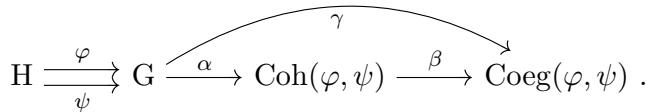
\includegraphics[keepaspectratio]{images/part002_030b7800.jpg}}

Throughout the rest of this section, \(n^{o}\), we assume that the frame of the pair \((\varphi,\psi)\) is a connected quiver and fix a vertex \(a_{0}\) of G. Consequently, the groupoids \(\mathrm{Coh}(\varphi,\psi)\) and \(\mathrm{Coeg}(\varphi,\psi)\) are transitive.

Denote by \(\Gamma\) the quiver \((\mathrm{Som}(\mathrm{G}), \mathrm{Som}(\mathrm{H}), \mathrm{Som}(\varphi), \mathrm{Som}(\psi))\) , \(\widetilde{\Gamma}\) the graph associated with \(\Gamma\), and let \(\Omega(\widetilde{\Gamma})\) be the set of finite sequences \((z_1, \ldots, z_n)\) of arrows of \(\widetilde{\Gamma}\) , with \(n \geqslant 1\) , such that the term of \(z_i\) is the origin of \(z_{i+1}\) if \(1 \leqslant i < n\) and that the term of \(z_n\) is the origin of \(z_1\) . In No. 1 we constructed a map \(\mathbf{z} \mapsto c(\mathbf{z})\) from the set \(\Omega(\widetilde{\Gamma})\) into the set of conjugacy classes of the group \(\mathrm{Coh}(\varphi, \psi)_{a_0}\) .

Denote by \(H \times_{G} H\) the equalizer in \(H \times H\) of the quiver morphisms \(\psi \circ pr_{1}\) and \(\varphi \circ pr_{2}\) . The set of its vertices is the set of pairs \((a, b)\) of vertices of H such that \(\psi(a) = \varphi(b)\) ; the set of its arrows is the set of pairs \((f, g)\) of arrows of H such that \(\psi(f) = \varphi(g)\) ; the origin of an arrow \((f, g)\) is the vertex \((o(f), o(g))\) and its endpoint is the vertex \((t(f), t(g))\) (cf. II, p. 153).

Finally, denote by \(\mathrm{Ker}(\varphi, \psi)\) the equalizer of \(\varphi\) and \(\psi\) ; recall (II, p. 165, example 2) that this is the subquiver of H whose vertices \(a\) are those such that \(\varphi(a) = \psi(a)\) and whose arrows are the \(f \in \mathrm{Fl}(\mathrm{H})\) such that \(\varphi(f) = \psi(f)\) .

PROPOSITION 4. --- Let \(\mu\colon\mathrm{H}\times_{\mathrm{G}}\mathrm{H}\to\mathrm{H}\) be a quiver morphism such that \(\varphi\circ\mu=\varphi\circ\mathrm{pr}_{1}\) and \(\psi\circ\mu=\psi\circ\mathrm{pr}_{2}\) . Suppose that, for every pair \((a,b)\) of vertices of H such that \(\varphi(a)=\varphi(b)\) , there exists a vertex \(c\) of H such that \(\varphi(c)=\psi(b)\) and \(a=\mu(b,c)\) .

  Let \(A_{1}\) be a set of vertices of \(\mathrm{Ker}(\varphi,\psi)\) meeting each of its connected components, and let \(Z_{1}\) be the set of elements of \(\Omega(\widetilde{\Gamma})\) of the form \(((a,1))\) , where \(a\in A_{1}\). Let \(A_{2}\) be a set of vertices of \(H\times_{G}H\) meeting every connected component of \(H\times_{G}H\) and let \(Z_{2}\) be the set of triples of the form \(((a,1),(b,1),(\mu(a,b),-1))\) , for \((a,b)\) ranging over \(A_{2}\) .

Then, \(\Omega(\widetilde{\Gamma})\) is the smallest distinguished subset of \(\Omega(\widetilde{\Gamma})\) which contains \(Z_1 \cup Z_2\). In particular, the conjugacy classes \(c(\mathbf{z})\) in \(\mathrm{Coh}(\varphi, \psi)_{a_0}\) , where \(\mathbf{z}\) runs through \(Z_1 \cup Z_2\) , generate the kernel of the canonical homomorphism \(\beta_{a_0}\) of \(\mathrm{Coh}(\varphi, \psi)_{a_0}\) to \(\mathrm{Coeg}(\varphi, \psi)_{\beta(a_0)}\) .

Denote by \(Z_{1}^{\prime}\) , \(Z_{2}^{\prime}\) and \(Z^{\prime}\) the smallest distinguished subsets of \(\Omega(\widetilde{\Gamma})\) respectively containing \(Z_{1}\) , \(Z_{2}\) and \(Z_{1} \cup Z_{2}\) (II, p. 197, def. 1). The aim is to prove that \(Z^{\prime}\) is equal to \(\Omega(\widetilde{\Gamma})\). By II, p. 199, corollary 1 of prop. 1 of II, p. 197, the last assertion of the proposition will follow from this.

Lemma 1. --- a) For every vertex \(a\) of \(\operatorname{Ker}(\varphi, \psi)\) , \(((a, 1))\) belongs to \(Z_1'\) .

\begin{enumerate}
\def\labelenumi{\alph{enumi})}
\setcounter{enumi}{1}
\item
  For every vertex \((a,b)\) of \(\mathrm{H}\times_{\mathrm{G}}\mathrm{H}\) , \(((a,1),(b,1),(\mu(a,b),-1))\) belongs to \(\mathbf{Z}_2^{\prime}\) .
\item
  Let \(A_{1}^{\prime}\) be the set of vertices \(a\) of \(\operatorname{Ker}(\varphi,\psi)\) such that \(((a,1))\) belongs to \(Z_{1}^{\prime}\) . We have \(A_{1}\subset A_{1}^{\prime}\) , by definition of \(Z_{1}^{\prime}\) . Let \(f\) be an arrow of \(\operatorname{Ker}(\varphi,\psi)\) , let \(a\) be its source and \(b\) its target. It follows from property (iv) in the definition of a distinguished subset (II, p. 197, def. 1) applied to the sequence \(((f,1))\) that \(a\in A_{1}^{\prime}\) is equivalent to \(b\in A_{1}^{\prime}\) . Since \(A_{1}\) meets every connected component of \(\operatorname{Ker}(\varphi,\psi)\) , we have \(A_{1}^{\prime}=\operatorname{Som}(\operatorname{Ker}(\varphi,\psi))\) , which is what had to be proved.
\item
  Let \(A_{2}^{\prime}\) be the set of vertices \((a,b)\) of \(H \times_{G} H\) such that the triple \(((a,1),(b,1),(\mu(a,b),-1))\) belongs to \(Z_{2}^{\prime}\) . By hypothesis, one has \(A_{2} \subset A_{2}^{\prime}\) . Since \(A_{2}\) meets each connected component of \(H \times_{G} H\) , it suffices to establish that, if there exists an arrow \((f,f^{\prime})\) joining a vertex \((a', b')\) to a vertex \((a, b)\) , then \((a, b)\) belongs to \(A_2'\) if and only if the same is true of \((a', b')\) .
\end{enumerate}

Let us set \(f'' = \mu(f, f')\) ; it is an arrow joining \(\mu(a', b')\) to \(\mu(a, b)\) and one has \(\varphi(f'') = \varphi(f)\) and \(\psi(f'') = \psi(f')\) . By condition (iv) in the definition of a distinguished subset of \(\Omega(\widetilde{\Gamma})\) (loc. cit.) applied to the sequence \(((f, 1), (f', 1), (f'', -1))\) , the two conditions

\begin{enumerate}
\def\labelenumi{(\roman{enumi})}
\item
  the triple \(((a,1),(b,1),(\mu (a,b), - 1))\) belongs to \(Z^{\prime}\) ;
\item
  the triple \(((a',1),(b',1),(\mu(a',b'),-1))\) belongs to \(Z'\) are equivalent. This shows that \((a,b)\) belongs to \(A_{2}'\) if and only if \((a',b')\) belongs to \(A_{2}'\) and concludes the proof of the lemma.
\end{enumerate}

We now prove by induction on the integer \(n \geqslant 1\) that every element \(((a_1, \varepsilon_1), (a_2, \varepsilon_2), \ldots, (a_n, \varepsilon_n))\) of \(\Omega(\widetilde{\Gamma})\) belongs to \(Z'\) .

\casehead{Case where \(n = 1\)}

Let \(((a,\varepsilon))\) be an element of \(\Omega(\tilde{\Gamma})\) of length 1. We have \(\varphi(a)=\psi(a)\) , whence \(((a,1))\in\mathbb{Z}'\). By Lemma 1, condition (ii) in the definition of a distinguished subset then implies that \(((a,-1))\) belongs to \(Z'\) .

\casehead{Case where \(n \geqslant 2\)}

By virtue of condition (ii) of a distinguished subset, it suffices to treat the case where \(\varepsilon_{2}=1\). Suppose that \(\varepsilon_{1}=1\) ; then, \((a_{1},a_{2})\) is a vertex of H \(\times_{G}H\) ; set \(a=\mu(a_{1},a_{2})\) ; by Lemma 1, the triple \(((a_{1},1),(a_{2},1),(a,-1))\) therefore belongs to \(Z'\). In the case where \(\varepsilon_{1}=-1\) , we have \(\varphi(a_{1})=\varphi(a_{2})\) ; one can therefore choose a vertex \(a\) of H such that \(\mu(a_{2},a)=a_{1}\) and the triple \(((a_{2},1),(a,1),(a_{1},-1))\) belongs to \(Z'\) , so the triple \(((a_{1},-1),(a_{2},1),(a,1))\) also belongs to \(Z'\), by virtue of condition (ii) in the definition of a distinguished subset.

Then, \(((a,\varepsilon_1),(a_3,\varepsilon_3),\ldots ,(a_n,\varepsilon_n))\) belongs to \(\Omega (\widetilde{\Gamma})\) and is of length \(n - 1\). By induction, this is an element of \(\mathbf{Z}'\) . Using conditions (i), (ii), and (iii) of the definition of a distinguished subset, we successively deduce that the elements

\[
\begin{array}{c} ((a _ {1}, \varepsilon_ {1}), (a _ {2}, 1), (a, - \varepsilon_ {1}), (a, \varepsilon_ {1}), (a _ {3}, \varepsilon_ {3}), \ldots , (a _ {n}, \varepsilon_ {n})), \\ ((a, - \varepsilon_ {1}), (a, \varepsilon_ {1}), (a _ {3}, \varepsilon_ {3}), \ldots , (a _ {n}, \varepsilon_ {n}), (a _ {1}, \varepsilon_ {1}), (a _ {2}, 1)), \\ ((a _ {3}, \varepsilon_ {3}), \ldots , (a _ {n}, \varepsilon_ {n}), (a _ {1}, \varepsilon_ {1}), (a _ {2}, 1)), \\ ((a _ {1}, \varepsilon_ {1}), (a _ {2}, 1), (a _ {3}, \varepsilon_ {3}), \ldots , (a _ {n}, \varepsilon_ {n})) \end{array}
\]

belong to Z'. This completes the proof of the proposition.

COROLLARY. --- a) With the notations of Proposition 4, suppose further that the map (Som(φ), Som(ψ)) from Som(H) into Som(G) × Som(G) is injective and that its image is the graph of an equivalence relation on Som(G). Then, for every vertex (a, b) of H \(\times_{G}\) H, there exists a unique vertex \(c_{a,b}\) of H such that \(\varphi(c_{a,b}) = \varphi(a)\) and \(\psi(c_{a,b}) = \psi(b)\) .

\begin{enumerate}
\def\labelenumi{\alph{enumi})}
\setcounter{enumi}{1}
\tightlist
\item
  Suppose further that for every arrow \((f, f')\) of H \(\times_{G}\) H, there exists an arrow \(f''\) of H such that \(\varphi(f'') = \varphi(f)\) and \(\psi(f'') = \psi(f')\) .
\end{enumerate}

Let A be a set of vertices of H \(\times_{G}\) H meeting each of its connected components. Then, the kernel of the morphism \(\beta_{a_{0}}\) is the smallest normal subgroup of \(\mathrm{Coh}(\varphi,\psi)_{a_{0}}\) which contains the conjugacy classes \(c((a,1),(b,1),(c_{a,b},-1))\) , for \((a,b)\in\mathrm{A}\) .

Let R be the equivalence relation on \(\operatorname{Som}(\mathrm{G})\) whose graph is the image of the mapping \((\operatorname{Som}(\varphi),\operatorname{Som}(\psi))\) . Let \((a,b)\) be a vertex of \(H\times_{G}H\) . One thus has \(\operatorname{R}\{\varphi(a),\psi(a)\}\) and \(\operatorname{R}\{\varphi(b),\psi(b)\}\) , whence \(\operatorname{R}\{\varphi(a),\psi(b)\}\) since \(\psi(a)=\varphi(b)\) . Hence, there exists a unique vertex \(c\) of H such that \(\varphi(c)=\varphi(a)\) and \(\psi(c)=\psi(b)\) ; it is denoted \(\mu(a,b)\) .

For every arrow \((f, f')\) of \(H\times_{G}H\), choose an arrow \(f''\) of H such that \(\varphi(f'') = \varphi(f)\) and \(\psi(f'') = \psi(f')\) and denote it \(\mu(f, f')\) .

We have thus defined a quiver morphism \(\mu\colon\mathrm{H}\times_{\mathrm{G}}\mathrm{H}\to\mathrm{H}\) such that \(\varphi\circ\mu=\varphi\circ\mathrm{pr}_{1}\) and \(\psi\circ\mu=\psi\circ\mathrm{pr}_{2}\) .

Let \((a,b)\) be a pair of vertices of H such that \(\varphi(a)=\varphi(b)\) . We have \(\mathrm{R}\{\varphi(a),\psi(a)\}\) and \(\mathrm{R}\{\varphi(b),\psi(b)\}\) , therefore \(\mathrm{R}\{\psi(b),\psi(a)\}\) . There consequently exists a unique vertex \(c\) of H such that \(\varphi(c)=\psi(b)\) and \(\psi(c)=\psi(a)\) . The vertex \(\mu(b,c)\) satisfies \(\varphi(\mu(b,c))=\varphi(b)=\varphi(a)\) and \(\psi(\mu(b,c))=\psi(c)=\psi(a)\) . We therefore have \(\mu(b,c)=a\) since the map \((\operatorname{Som}(\varphi),\operatorname{Som}(\psi))\) of \(\operatorname{Som}(\operatorname{H})\) into \(\operatorname{Som}(\operatorname{G})\times\operatorname{Som}(\operatorname{G})\) is injective.

Let \(A_{1}\) be the set of vertices of \(\operatorname{Ker}(\varphi,\psi)\) and let \(Z_{1}\) be the set of elements of \(\Omega(\widetilde{\Gamma})\) of the form \(((a,1))\) , for \(a\in A_{1}\) . Set \(A_{2}=A\) and let \(Z_{2}\) be the set of elements \(((a,1),(b,1),(\mu(a,b),-1))\) of \(\Omega(\widetilde{\Gamma})\) , for \((a,b)\in A_{2}\) . Denote by \(\widetilde{Z}\) (resp. \(\widetilde{Z}_{1}\), respectively \(\widetilde{Z}_{2}\)) the smallest distinguished subset of \(\Omega(\widetilde{\Gamma})\) containing \(Z_{1}\cup Z_{2}\) (resp. \(Z_{1}\), respectively \(Z_{2}\)).

Let \(a \in \mathrm{A}_1\). We have \(\varphi(a) = \psi(a)\) ; set \(x = \varphi(a)\). The vertex \(a\) is the unique vertex of H such that \(\varphi(a) = \psi(a) = x\). In particular, we have \(\mu(a, a) = a\). The triple \(((a, 1), (a, 1), (a, -1))\) therefore belongs to \(\mathbf{Z}_2\). It then follows from conditions (i) and (iii) in the definition of a distinguished subset that \(((a, 1))\) belongs to \(\widetilde{\mathbf{Z}}_2\). Consequently, we have \(\mathbf{Z}_1 \subset \widetilde{\mathbf{Z}}_2\) , whence \(\widetilde{\mathbf{Z}} = \widetilde{\mathbf{Z}}_2\) .

By Proposition 4, \(\Omega(\tilde{\Gamma})\) is the smallest distinguished subset of \(\Omega(\tilde{\Gamma})\) containing \(Z_{2}\), and the kernel of \(\beta_{a_{0}}\) is the smallest normal subgroup of \(\mathrm{Coh}(\varphi,\psi)_{a_{0}}\) which contains the conjugacy classes \(c(\mathbf{z})\) , for \(\mathbf{z}\in Z_{2}\) . Hence the corollary.

Example. --- Let X and R be topological spaces, let o and t be continuous maps from R to X, and let C be the set of pairs \((f,g)\in\mathrm{R}^{2}\) such that \(t(f)=o(g)\) in R and let m be a continuous map from C to R that makes the quiver \((\mathrm{X},\mathrm{R},o,t)\) a groupoid; suppose further that the map \(f\mapsto f^{-1}\) from R to R is continuous. The hypotheses of the proposition are then satisfied if one sets \(\mathrm{H}=\varpi(\mathrm{R})\) , \(\mathrm{G}=\varpi(\mathrm{X})\) , \(\varphi=\varpi(o)\) , \(\psi=\varpi(t)\) and \(\mu=\varpi(m)\) .

Suppose further that R is the graph of an equivalence relation on X, with the maps o and t being derived from the projections of \(X \times X\) in X by passing to subspaces. The hypotheses of the corollary are then satisfied.

Remark. --- *More generally, the hypotheses of the proposition are satisfied when (G, H, \(\varphi\) , \(\psi\) , \(\mu\) ) is a “groupoid of groupoids.” This means that G and H are groupoids, \(\varphi\) and \(\psi\) are morphisms of groupoids from H to G, making the quadruple (G, H, \(\varphi\) , \(\psi\) ) a “groupoid quiver”; finally, \(\mu\) is a composition law in this “quiver” given by a groupoid morphism H \(\times_{\mathrm{G}}\) H → H, satisfying a certain number of properties expressing the associativity of the law and the fact that every “arrow” is invertible. The reader will also note that the applications to the fundamental groupoid studied in this work all fall within this case.

\subsection{Isotropy group of a coequalizer}

Let G and H be groupoids; let \(\varphi\) and \(\psi\) morphisms of groupoids from H to G. The purpose of this section is to summarize the computation of the isotropy groups of the cohomotoper (II, p. 193, prop. 6) and the comparison of the isotropy groups of the cohomotoper and of the coequalizer made in the preceding section, in order to deduce from this the computation of the isotropy groups of the coequalizer Coeg( \(\varphi\) , \(\psi\) ).

Denote by \(\alpha\colon\mathrm{G}\to\mathrm{Coh}(\varphi,\psi)\) , \(\beta\colon\mathrm{Coh}(\varphi,\psi)\to\mathrm{Coeg}(\varphi,\psi)\) and \(\gamma=\beta\circ\alpha\colon\mathrm{G}\to\mathrm{Coeg}(\varphi,\psi)\) the canonical groupoid morphisms. Denote \(h\colon\mathrm{Som}(\mathrm{H})\to\mathrm{Fl}(\mathrm{Coh}(\varphi,\psi))\) the canonical homotopy; recall that the set of vertices of \(\mathrm{Coh}(\varphi,\psi)\) is equal to \(\mathrm{Som}(\mathrm{G})\) .

Denote by \(\Gamma\) the quiver (Som(G), Som(H), Som(φ), Som(ψ)), denote then \(\varphi_0\) and \(\psi_0\) the maps induced by \(\varphi\) and \(\psi\) by passing to orbits and \(\Gamma_0\) the frame (Orb(G), Orb(H), \(\varphi_0, \psi_0\) ) of the pair ( \(\varphi, \psi\) ). We shall assume that the quiver \(\Gamma_0\) is connected and its vertex set is nonempty, which amounts to assuming that the groupoids Coh(φ, ψ) and Coeg(φ, ψ) are transitive.

Recall (cf. II, p. 192, definition 4) that a base equipment consists of the data of a family \((a, b, c_1, c_2, \mathrm{T}, i_0)\) where: for all \(i \in \mathrm{Orb}(\mathrm{G})\) , \(a(i)\) is a vertex in the orbit \(i\) of \(\mathrm{G}\) ; for every \(j \in \mathrm{Orb}(\mathrm{H})\) , \(b(j)\) is a vertex in the orbit \(j\) of \(\mathrm{H}\) , \(c_1(j)\) and \(c_2(j)\) are arrows from \(\mathrm{G}\) respectively \(\varphi(b(j))\) to \(a(\varphi_0(j))\) and \(\psi(b(j))\) to \(a(\psi_0(j))\) ; \(\mathrm{T}\) is a subquiver of \(\Gamma_0\) whose associated tree is a maximal tree of the graph \(\widetilde{\Gamma}_0\) ; finally, \(i_0\) is an orbit of \(\mathrm{G}\) and we set \(a_0 = a(i_0)\) .

We then define a quiver morphism \(\tau_0\) from \(\Gamma_0\) to \(\mathrm{Coh}(\varphi, \psi)\) such that \(\tau_0(i) = \beta(a(i))\) and \(\tau_0(j) = \alpha(c_1(j))^{-1}h(b(j))\alpha(c_2(j))\) for \(i \in \mathrm{Orb}(\mathrm{G})\) and \(j \in \mathrm{Orb}(\mathrm{H})\) . If \(i\) belongs to \(\mathrm{Orb}(\mathrm{G})\) , let \(d_i\) be the unique class of paths in the graph \(\widetilde{\mathrm{T}}\) connecting \(i_0\) to \(i\) and denote by \(\delta_i\) its image in \(\mathrm{Coh}(\varphi, \psi)\) by the groupoid morphism \(\tau_0\) .

From these data, prop. 6 (II, p. 193) yields a surjective homomorphism.

\[
\Lambda \colon \bigl (\underset {i \in \pi_ {0} (\mathrm{G})} {*} \mathrm{G} _ {a (i)} \bigr) * \mathrm{F} (\operatorname{Orb} (\mathrm{H})) \to \operatorname{Coh} (\varphi , \psi) _ {a (i _ {0})}
\]

and describes generators of its kernel, thereby providing a presentation of the group \(\mathrm{Coh}(\varphi,\psi)_{a_{0}}\) .

The set of loops of length \(\geqslant 1\) in the graph \(\widetilde{\Gamma}\) associated with \(\Gamma\) is identified with the set \(\Omega(\widetilde{\Gamma})\) of sequences \((z_1, \ldots, z_n)\) of arrows of \(\widetilde{\Gamma}\) , indexed by \(\mathbf{Z}/n\mathbf{Z}\) , where \(n\) runs through the set of integers \(\geqslant 1\) , such that for every \(k \in \mathbf{Z}/n\mathbf{Z}\) , the term of \(z_k\) is the origin of \(z_{k+1}\) . Let \(\mathbf{Z}\) be a subset of \(\Omega(\widetilde{\Gamma})\) such that the conjugacy classes \(c(z)\) , for \(z \in \mathbf{Z}\) , generate the kernel of the surjective homomorphism \(\beta_{a_0}\) . The homomorphism \(\beta_{a_0} \circ \Lambda\) is surjective; to deduce its kernel from this, that is, a presentation of the group \(\operatorname{Coeg}(\varphi, \psi)_{\beta(a_0)}\) , it remains to choose, for every \(z \in \mathbf{Z}\) , an element \(\mathrm{C}(z)\) in the group \(\left( \begin{array}{cc} * & \mathrm{G}_{a(i)} \\ i \in \mathrm{Orb}(\mathrm{G}) & \end{array} \right) * \mathrm{F}(\pi_0(\mathrm{H}))\) such that \(\Lambda(\mathrm{C}(z))\) belongs to the conjugacy class \(c(z)\) .

So let \(z = (z_{1}, \ldots, z_{n})\) be an element of \(\Omega(\tilde{\Gamma})\) ; set \(z_{k} = (y_{k}, \varepsilon_{k})\) , where \(y_{k} \in \mathrm{Fl}(\Gamma) = \mathrm{Som}(\mathrm{H})\) and \(\varepsilon_{k} \in \{\pm 1\}\) . By definition, \(c(z)\) is the conjugacy class of the element

\[
g h (y _ {1}) ^ {\varepsilon_ {1}} \dots h (y _ {n}) ^ {\varepsilon_ {n}} g ^ {- 1}
\]

of the group \(\mathrm{Coh}(\varphi,\psi)_{a_{0}}\) , where g is an arbitrary arrow in \(\mathrm{Coh}(\varphi,\psi)\) connecting \(a_{0}\) to the origin of \(z_{1}\) . For \(k \in Z/nZ\) , let \(j_{k}\) be the orbit of \(y_{k}\) in H and choose an arrow \(f_{k}\) of H connecting \(y_{k}\) to the vertex \(b(j_{k})\). By definition of a homotopy, we then have the relation

\[
h (y _ {k}) (\alpha \circ \psi) (f _ {k}) = (\alpha \circ \varphi) (f _ {k}) h (b (j _ {k}))
\]

in the groupoid \(\mathrm{Coh}(\varphi,\psi)\) . Consequently, using the definition of the quiver morphism \(\tau_{0}\) , we have

\[
\begin{array}{l} h (y _ {k}) = (\alpha \circ \varphi) (f _ {k}) \cdot h (b (j _ {k})) \cdot (\alpha \circ \psi) (f _ {k}) ^ {- 1} \\ \quad = (\alpha \circ \varphi) (f _ {k}) \cdot (\alpha \circ c _ {1}) (j _ {k}) \cdot \tau_ {0} (j _ {k}) \cdot (\alpha \circ c _ {2}) (j _ {k}) ^ {- 1} \cdot (\alpha \circ \psi) (f _ {k}) ^ {- 1} \\ \quad = (\alpha \circ \varphi) (f _ {k}) \cdot (\alpha \circ c _ {1}) (j _ {k}) \cdot \delta_ {\varphi_ {0} (j _ {k})} ^ {- 1} \cdot \\ \quad \cdot \delta_ {\varphi_ {0} (j _ {k})} \cdot \tau_ {0} (j _ {k}) \cdot \delta_ {\psi_ {0} (j _ {k})} ^ {- 1} \cdot \\ \quad \cdot \delta_ {\psi_ {0} (j _ {k})} \cdot (\alpha \circ c _ {2}) (j _ {k}) ^ {- 1} \cdot (\alpha \circ \psi) (f _ {k}) ^ {- 1} \\ = u _ {k} \Lambda (j _ {k}) v _ {k}, \end{array}
\]

where we have set

\[
u _ {k} = \alpha (\varphi (f _ {k}) c _ {1} (j _ {k})) \cdot \delta_ {\varphi_ {0} (j _ {k})} ^ {- 1} \quad \text { and } \quad v _ {k} = \delta_ {\psi_ {0} (j _ {k})} \cdot \alpha (\psi (f _ {k}) c _ {2} (j _ {k})) ^ {- 1}.
\]

For every element \(k \in \mathbf{Z}/n\mathbf{Z}\) , define arrows \(\widetilde{u}_{k}, \widetilde{v}_{k}\) in G by

\[
h (y _ {k}) ^ {\varepsilon_ {k}} = \widetilde {u} _ {k} \Lambda (j _ {k}) ^ {\varepsilon_ {k}} \widetilde {v} _ {k},
\]

so that

\[
(\widetilde {u} _ {k}, \widetilde {v} _ {k}) = \left\{ \begin{array}{l l} (u _ {k}, v _ {k}) & \text { if } \varepsilon_ {k} = 1; \\ (v _ {k} ^ {- 1}, u _ {k} ^ {- 1}) & \text { if } \varepsilon_ {k} = - 1. \end{array} \right.
\]

Denote by \(x_{k}\) the origin of the arrow \(h(y_{k})^{\varepsilon_{k}}\) ; its target is then \(x_{k+1}\) ; let \(i_{k}\) be the orbit of \(x_{k}\) . Let us then define a loop \(\lambda_{k}(z)\) at \(a(i_{k})\) in the groupoid G by the formula

\[
\lambda_ {k} (z) = \left\{ \begin{array}{l l} c _ {2} (j _ {k - 1}) ^ {- 1} \psi (f _ {k - 1}) ^ {- 1} \varphi (f _ {k}) c _ {1} (j _ {k}) & \text {if} (\varepsilon_ {k - 1}, \varepsilon_ {k}) = (1, 1); \\ c _ {2} (j _ {k - 1}) ^ {- 1} \psi (f _ {k - 1}) ^ {- 1} \psi (f _ {k}) c _ {2} (j _ {k}) & \text {if} (\varepsilon_ {k - 1}, \varepsilon_ {k}) = (1, - 1); \\ c _ {1} (j _ {k - 1}) ^ {- 1} \varphi (f _ {k - 1}) ^ {- 1} \varphi (f _ {k}) c _ {1} (j _ {k}) & \text {if} (\varepsilon_ {k - 1}, \varepsilon_ {k}) = (- 1, 1); \\ c _ {1} (j _ {k - 1}) ^ {- 1} \varphi (f _ {k - 1}) ^ {- 1} \psi (f _ {k}) c _ {2} (j _ {k}) & \text {if} (\varepsilon_ {k - 1}, \varepsilon_ {k}) = (- 1, - 1) \end{array} \right.\tag{1}
\]

By construction, we have

\[
\Lambda (\lambda_ {k} (z)) = \widetilde {v} _ {k - 1} \widetilde {u} _ {k},
\]

so that the image under the homomorphism \(\Lambda\) of the element

\[
\mathrm{C} (z) = \lambda_ {1} (z) (j _ {1}) ^ {\varepsilon_ {1}} \lambda_ {2} (z) (j _ {2}) ^ {\varepsilon_ {2}} \dots \lambda_ {n} (z) (j _ {n}) ^ {\varepsilon_ {n}}\tag{2}
\]

belongs to the conjugacy class \(c(z)\) .

DEFINITION 3. --- Let G and H be groupoids; let \(\varphi\) and \(\psi\) morphisms of groupoids from H to G. We assume that the groupoid Coeg \((\varphi, \psi)\) is transitive. Let \((a, b, c_1, c_2, T, i_0)\) be a basic equipment of the pair \((\varphi, \psi)\) .

One calls complementary equipment the data of a subset Z of \(\Omega(\widetilde{\Gamma})\) such that the conjugacy classes \(c(\mathbf{z})\) for \(\mathbf{z} \in \mathbf{Z}\) generate the kernel of the homomorphism \(\beta_{a(i_0)}\) and, for every element \(\mathbf{z} = ((y_1, \varepsilon_1), \ldots, (y_n, \varepsilon_n))\) of Z, a sequence \(f(\mathbf{z}) = (f_1, \ldots, f_n)\) of arrows in H such that \(f_k\) connects \(y_k\) to the vertex \(b(j_k)\) , \(j_k\) denoting the orbit of \(y_k\) in H.

A complete equipment of the pair \((\varphi,\psi)\) is the data of a base equipment and a complementary equipment.

PROPOSITION 5. --- Let G and H be groupoids; let \(\varphi\) and \(\psi\) be morphisms of groupoids from H to G. Suppose that the groupoid \(\operatorname{Coeg}(\varphi, \psi)\) is transitive. Denote by \(\gamma\colon \mathrm{G} \to \mathrm{Coeg}(\varphi, \psi)\) the canonical groupoid morphism.

We equip the pair \((\varphi, \psi)\) with a complete equipment

\[
(a, b, c _ {1}, c _ {2}, \mathrm{T}, i _ {0}, \mathrm{Z}, (f (\mathbf {z})) _ {\mathbf {z} \in \mathrm{Z}}).
\]

For \(j \in \text{Orb(H)}\) , let \(\varphi_j \colon \text{H}_{b(j)} \to \text{G}_{a(\varphi_0(j))}\) and \(\psi_j \colon \text{H}_{b(j)} \to \text{G}_{a(\psi_0(j))}\) be the group homomorphisms \(\text{Int}(c_1(j))^{-1} \circ \varphi_{b(j)}\) and \(\text{Int}(c_2(j))^{-1} \circ \psi_{b(j)}\) respectively, where \(\varphi_0\) and \(\psi_0\) denote the canonical maps induced by \(\varphi\) and \(\psi\) by passing to orbits. Let \(\tau\) be the morphism of the frame \(\Gamma_0\) of the pair \((\varphi, \psi)\) into \(\text{Coeg}(\varphi, \psi)\) defined by \(\text{Som}(\tau)(i) = \gamma(a(i))\) if \(i \in \text{Orb(G)}\) and such that \(\text{Fl}(\tau)(j)\) is the path \(\gamma(c_1(j))^{-1} \gamma(c_2(j))\) in \(\text{Coeg}(\varphi, \psi)\). If \(i\) is an orbit of G, let \(c_i\) be the unique class of paths in \(\widetilde{\text{T}}\) connecting \(i_0\) to \(i\), and set \(\delta_i = \widetilde{\tau}(c_i)\) , where \(\widetilde{\tau} \colon \text{Grp(G)} \to \text{Coeg}(\varphi, \psi)\) is the canonical groupoid morphism induced by \(\tau\) .

There then exists a unique group homomorphism

\[
\lambda \colon \bigl ( \begin{array}{c} * \\ i \in \operatorname{Orb} (\mathrm{G}) \end{array} \mathrm{G} _ {a (i)} \bigr) * \mathrm{F} (\operatorname{Orb} (\mathrm{H})) \to \operatorname{Coeg} (\varphi , \psi) _ {\gamma (a (i _ {0}))}
\]

such that

\[
\begin{array}{l l} \lambda (f) = \delta_ {i} \gamma_ {a (i)} (f) \delta_ {i} ^ {- 1} & \text { for } i \in \mathrm{Orb(G)} \text { and } f \in \mathrm{G} _ {a (i)}, \\ \lambda (j) = \delta_ {\varphi_ {0} (j)} \tau (j) \delta_ {\psi_ {0} (j)} ^ {- 1} & \text { for } j \in \mathrm{Orb(H)}. \end{array}
\]

The homomorphism \(\lambda\) is surjective; its kernel is the smallest normal subgroup containing the following elements:

\[
\left(\mathrm{R} _ {1}\right) \quad r _ {1} (j) = j \quad \text { for } j \text { in } \mathrm{Fl} (\mathrm{T});
\]

\[
(\mathrm{R} _ {2}) \quad r _ {2} (j, f) = \varphi_ {j} (f) j \psi_ {j} (f) ^ {- 1} j ^ {- 1}
\]

\[
\text { for } j \in \operatorname{Orb} (\mathrm{H}) \text { and } f \in \mathrm{H} _ {b (j)};\tag{\((R_{3})\)}
\]

\[
r _ {3} (z) = \lambda_ {1} (z) j _ {1} ^ {\varepsilon_ {1}} \lambda_ {2} (z) j _ {2} ^ {\varepsilon_ {2}} \dots \lambda_ {n} (z) j _ {n} ^ {\varepsilon_ {n}}
\]

\[
\text { for } z = ((y _ {1}, \varepsilon_ {1}), \dots , (y _ {n}, \varepsilon_ {n})) \in \mathbf {Z},
\]

where the loops \(\lambda_{i}(z)\) are defined by formula (1), p. 208.

The existence and uniqueness of such a morphism follows from the universal property of the free product of a family of groups (A, I, p. 85, prop. 8). Denote by \(\alpha\colon G\to\mathrm{Coh}(\varphi,\psi)\) and \(\beta\colon\mathrm{Coh}(\varphi,\psi)\to\mathrm{Coeg}(\varphi,\psi)\) the canonical morphisms, so that \(\gamma=\beta\circ\alpha\). Let also \(h\colon\mathrm{Som}(H)\to\mathrm{Fl}(\mathrm{Coh}(\varphi,\psi))\) be the canonical homotopy relating \(\alpha\circ\varphi\) to \(\alpha\circ\psi\) . Since \(\beta\) is the groupoid morphism obtained by contracting the arrows of the image of \(h\) , we have

\[
\operatorname{Fl} (\tau) (j) = \gamma (c _ {1} (j)) ^ {- 1} \gamma (c _ {2} (j)) = \gamma (c _ {1} (j) ^ {- 1}) \beta (h (j)) \gamma (c _ {2} (j)) = \beta (\tau_ {0} (j))
\]

in \(\operatorname{Coeg}(\varphi,\psi)\) , where \(\tau_{0}\colon\Gamma_{0}\to\mathrm{Coh}(\varphi,\psi)\) denotes the quiver morphism induced by the base equipment \((a,b,c_{1},c_{2},\mathrm{T},i_{0})\) . Consequently, the homomorphism \(\lambda\) is the composite of the homomorphism \(\Lambda\) defined in Prop. 6 (II, p. 193) and of the surjective homomorphism \(\beta_{a(i_0)}\) . It is in particular surjective.

Let \(z \in \mathbf{Z}\). By construction, \(\Lambda(r_3(z))\) belongs to the conjugacy class \(c(z)\) . By definition of a complementary equipment, the kernel of the homomorphism \(\beta_{a(i_0)}\) is therefore the smallest normal subgroup of \(\mathrm{Coh}(\varphi, \psi)_{a(i_0)}\) containing the elements \(\Lambda(r_3(z))\) for \(z \in \mathbf{Z}\) . Since the homomorphism \(\Lambda\) is surjective, the kernel of the homomorphism \(\lambda = \beta_{a(i_0)} \circ \Lambda\) is therefore the smallest normal subgroup of the group \(\left( *_{i \in \mathrm{Orb}(G)} G_{a(i)} \right) * F(\pi_0(H))\) containing the generators of the kernel of \(\Lambda\) given by the formulas \((R_1), (R_2)\) , as well as the elements defined by the formulas \((R_3)\) . The proposition is thus proved.

\subsection{Quotient of a groupoid by the action of a group}

Let G be a transitive groupoid, let K be a group, and let \(\theta\colon\mathrm{K}\to\mathrm{Aut}(\mathrm{G})^{\circ}\) be a group homomorphism from K into the opposite group of the automorphism group of the groupoid G. We will say that the group K acts on the right on G. If \(k\in\mathrm{K}\) we will sometimes denote by \(k^{*}x\) (resp. \(k^{*}f\) ) the image of a vertex \(x\) (resp. of an arrow \(f\) ) of G under the groupoid automorphism \(\theta(k)\) .

Let \(|\mathrm{K}|\) be the groupoid whose set of vertices is \(\mathrm{K}\) and whose set of arrows connecting two vertices is empty if these vertices are distinct, and is reduced to a single element otherwise. Let \(\mathrm{H}\) be the product groupoid \(\mathrm{G} \times |\mathrm{K}|\) ; a vertex of \(\mathrm{H}\) is a pair \((a,k)\) , where \(a\) is a vertex of \(\mathrm{G}\) and \(k\) is an element of \(\mathrm{K}\) ; if \(f\) is an arrow of \(\mathrm{G}\) joining a vertex \(a\) to a vertex \(b\) , we shall denote \((f,k)\) the unique arrow of \(\mathrm{H}\) connecting \((a,k)\) to \((b,k)\) . Let \(\varphi: \mathrm{H} \to \mathrm{G}\) be the groupoid morphism given by the first projection, and let \(\psi: \mathrm{H} \to \mathrm{G}\) be the groupoid morphism such that \(\operatorname{Som}(\psi)((a,k)) = k^*a\) and \(\operatorname{Fl}(\psi)((f,k)) = k^*f\) if \(k \in \mathrm{K}\) , \(a \in \operatorname{Som}(\mathrm{G})\) and \(f \in \operatorname{Fl}(\mathrm{G})\) .

Let G/K denote the coequalizer \(\operatorname{Coeg}(\varphi,\psi)\) and let \(\gamma\colon G\to G/K\) be the canonical groupoid morphism.

Let o be a vertex of G. For \(k \in K\), choose an arrow \(c_{k}\) connecting \(k^{*}o\) to o in G; such an arrow exists because G is transitive. For \(k \in K\), denote by \(\text{Fix}(k)\) the subgroupoid of G whose vertices (resp. arrows) are the elements of \(\text{Som}(G)\) (resp. of \(\text{Fl}(G)\) ) fixed by k; let us choose a set \(A_{k}\) of vertices of \(\text{Fix}(k)\) meeting all the orbits of this groupoid. For \(k \in K\) and \(a \in A_{k}\) we also choose an arrow \(f_{(a,k)}\) in G connecting the vertex a to the vertex o.

Proposition 6. — The unique group homomorphism

\[
\lambda \colon \mathrm{G} _ {o} * \mathrm{F} (\mathrm{K}) \to (\mathrm{G} / \mathrm{K}) _ {\gamma (o)}
\]

such that \(\lambda(f) = \gamma_o(f)\) for \(f \in \mathrm{G}_o\) and \(\lambda([k]) = \gamma(c_k)\) for \(k \in \mathrm{K}\) is surjective. Its kernel is the smallest normal subgroup of \(\mathrm{G}_o * \mathrm{F}(\mathrm{K})\) containing the following elements:

\[
r _ {2} (k, f) = [ k ] ^ {- 1} f [ k ] (c _ {k} ^ {- 1} k ^ {*} (f) ^ {- 1} c _ {k})\tag{\((R_{2})\)}
\]

\[
\text { for } k \in \mathrm{K} \text { and } f \in \mathrm{G} _ {o};\tag{\((\mathrm{R}_{3}^{\prime})\)}
\]

\[
r _ {3} ^ {\prime} (k, a) = [ k ] (c _ {k} ^ {- 1} k ^ {*} (f _ {(a, k)}) ^ {- 1} f _ {(a, k)}))
\]

\[
\text { for } k \in \mathrm{K} - \{e \} \text { and } a \in \mathrm{A} _{k}\tag{\((\mathrm{R}_{3}^{\prime\prime})\)}
\]

\[
r _ {3} ^ {\prime \prime} (k, h) = [ k h ] ^ {- 1} [ k ] [ h ] (c _ {h} ^ {- 1} h ^ {*} (c _ {k} ^ {- 1}) c _ {k h})
\]

\[
\text { for } k,h \in \mathrm{K}.
\]

Since G is transitive, the map which associates to an element \(k \in K\) the orbit of \((o, k)\) is a bijection from K onto the set of orbits of H. We thus identify \(\operatorname{Orb}(\mathbf{G})\) with \(\{o\}\) and \(\operatorname{Orb}(\mathbf{H})\) with K. The frame \(\Gamma_{0}\) of the pair \((\varphi, \psi)\) then identifies with the quiver having a single vertex o and whose set of arrows is K. Let T be the subquiver of \(\Gamma_{0}\) of vertex set \(\{o\}\) and whose set of arrows is empty; the associated graph is the unique maximal tree of the graph \(\widetilde{\Gamma}_{0}\).

The family \((o,(o,k)_{k\in \mathrm{K}},(e_o)_{k\in \mathrm{K}},(c_k)_{k\in \mathrm{K}},\mathrm{T},o)\) is a base equipment of the pair \((\varphi ,\psi)\) .

The map \(f \mapsto (f, k)\) defines an isomorphism of the isotropy group \(G_o\) onto the isotropy group \(H_{(o,k)}\) ; under this isomorphism, the homomorphisms \(\varphi_k\) and \(\psi_k\) of \(H_{(o,k)}\) into \(G_o\) defined by prop. 5 of II, p. 208 are given by

\[
\varphi_ {k} (f, k) = f \quad \text { and } \quad \psi_ {k} (f, k) = c _ {k} ^ {- 1} k ^ {*} (f) c _ {k},\tag{3}
\]

for \(k\in \mathrm{K}\) and \(f\in \mathrm{G}_o\).

The quiver \(H \times_{G} H\) is the equalizer in \(H \times H\) of quiver morphisms \(\psi \circ pr_{1}\) and \(\varphi \circ pr_{2}\) . Its vertices are the pairs \(((a, k), (b, h))\) where a and b are vertices of G and k and h are elements of K such that \(b = k^{*}a\) , and its arrows are the pairs \(((f, k), (g, h))\) where f and g are arrows of G, and k and h are elements of K such that \(g = k^{*}f\) ; the origin of the arrow \(((f,k),(g,h))\) is equal to \(((o(f),k),(o(g),h))\) ; its target is equal to \(((t(f),k),(t(g),h))\) .

We then define a quiver morphism \(\mu\) of \(H \times_{\mathrm{G}} H\) into H by setting \(\mu((a,k),(b,h)) = (a,kh)\) and \(\mu((f,k),(g,h)) = (f,kh)\) . We have \(\varphi \circ \mu = \varphi \circ \mathrm{pr}_1\) and \(\psi \circ \mu = \psi \circ \mathrm{pr}_2\) .

Let \(x\) and \(y\) be vertices of H such that \(\varphi(x) = \varphi(y)\). There thus exists a vertex \(a\) of G and elements \(k\) and \(h\) of K such that \(x = (a, k)\) and \(y = (a, h)\) . Set \(z = (h^* a, h^{-1} k)\) ; we have \(\mu(y, z) = x\). This shows that the pair \((\varphi, \psi)\) satisfies the hypotheses of Prop. 4 (II, p. 202).

A vertex \((a,k)\) of H belongs to the groupoid \(\operatorname{Ker}(\varphi,\psi)\), equalizer of \(\varphi\) and \(\psi\), if and only if \(k^{*}a=a\), that is, if k belongs to the stabilizer of the vertex a in the group K. Let \(A_{1}\) be the set of pairs \((a,k)\), for \(k\in K\) and \(a\in A_{k}\); it meets all the orbits of the subgroupoid \(\operatorname{Ker}(\varphi,\psi)\) of H. Let \(Z_{1}\) be the part of \(\Omega(\widetilde{\Gamma})\) formed of sequences of the form (((a,k),1)), for \((a,k)\in A_{1}\). For \(\mathbf{z}=((a,k),1)\in\mathbf{Z}_{1}\), \((f_{(a,k)},k)\) is an arrow of H which connects \((a,k)\) to \((o,k)\). Set \(f(\mathbf{z})=((f_{(a,k)},k))\).

The set \(\mathrm{A}_2\) of vertices of \(\mathrm{H} \times_{\mathrm{G}} \mathrm{H}\) of the form \(((o,k), (k^*o,h))\) , for \((k,h) \in \mathrm{K}^2\) , meets every orbit of \(\mathrm{H} \times_{\mathrm{G}} \mathrm{H}\) . Observe also that one has \(\mu((o,k), (k^*o,h)) = (o,kh)\) . The arrows \((e_o,k), (c_k,h), (e_o,kh)\) in H connect respectively \((o,k), (k^*o,h), (o,kh)\) to \((o,k), (o,h)\) and \((o,kh)\) . Denote by \(\mathrm{Z}_2\) the set of sequences of the form \((((o,k),1), ((k^*o,h), 1), ((o,kh), -1))\) in \(\Omega(\widetilde{\Gamma})\) ; for such an element \(\mathbf{z}\) of \(\mathrm{Z}_2\) , set \(f(\mathbf{z}) = ((e_o,k), (c_k,h), (e_o,kh))\) .

By prop. 4 of II, p. 202, the set \(Z = Z_1 \cup Z_2\) and the family \((f(\mathbf{z}))_{z \in \mathbb{Z}}\) form a complementary equipment.

Let \(k \in \mathrm{K}\) and let \(a \in \mathrm{A}_k\) . The element \(\mathrm{C}((a, k), 1)\) of the group \(\mathrm{G}_o * \mathrm{F}(\mathrm{K})\) defined by formula (2) of II, p. 208 is equal to

\[
c _ {k} ^ {- 1} \psi ((f _ {(a, k)}, k)) ^ {- 1} \varphi (f _ {(a, k)}) e _ {o} [ k ] = (c _ {k} ^ {- 1} k ^ {*} (f _ {(a, k)}) ^ {- 1} f _ {(a, k)}) [ k ].\tag{4}
\]

Let \(k,h \in \mathbf{K}\). One verifies that the element

\[
\mathrm{C} (((o, k), 1), ((k ^ {*} o, h), 1), ((o, k h), - 1))
\]

of the group \(G_{o} * F(K)\) defined by formula (2) of II, p. 208 is equal to

\[
[ k ] [ h ] (c _ {h} ^ {- 1} h ^ {*} (c _ {k} ^ {- 1}) c _ {k h}) [ k h ] ^ {- 1}.\tag{5}
\]

The elements \(r_3'(e, a)\) given by the relations \((\mathrm{R}_3')\) for \(k = e\) are all equal to \([e]c_e^{-1}\), an element of the group \(\mathrm{G}_o * \mathrm{F}(\mathrm{K})\) obtained by applying the relation \((\mathrm{R}_{3}^{\prime\prime})\) to \(k = h = e\). In view of relations (3), (4), and (5), the proposition therefore follows from II, p. 208, prop. 5.

COROLLARY 1. --- Suppose that the group K is generated by the fixators of the vertices of G. Then the group homomorphism \(\gamma_{o}\colon\mathrm{G}_{o}\to(\mathrm{G}/\mathrm{K})_{\gamma(o)}\) is surjective. Moreover, if the groupoid G is simply transitive, then so is the groupoid G/K.

The relation \((\mathrm{R}_{3}^{\prime\prime})\) implies \(\lambda([e]) = \lambda(c_{e}) = \gamma_{o}(c_{e})\) . The relations \((\mathrm{R}_{3}^{\prime\prime})\) then imply that the set of \(k \in K\) such that \(\lambda([k])\) belongs to the image of \(\gamma_{o}\) is a subgroup of K. Finally, the relations \((\mathrm{R}_{3}^{\prime})\) show that, for every element \(k \in K\) whose fixator is not empty, \(\lambda([k])\) belongs to the image of \(\gamma_{o}\) . The corollary follows from this.

Remark 1. --- One can give another description, sometimes more convenient, of the group \((\mathrm{G}/\mathrm{K})_{\gamma(o)}\). For this, set \(M = K \times G_{o}\) and let us define a composition law on M by the formula

\[
(k, a) \cdot (h, b) = (k h, c _ {k h} ^ {- 1} h ^ {*} (c _ {k} a) c _ {h} b),
\]

for \(k\) , \(h \in \mathrm{K}\) and \(a\) , \(b \in \mathrm{G}_o\) . We verify that this composition law is associative, that \((e, c_e^{-1})\) is an identity element and that the element \((k^{-1}, c_{k^{-1}}^{-1}(k^{-1})^*(c_k a)^{-1} c_e)\) is the inverse of \((k, a)\) . It therefore endows M with a group structure. Moreover, the map \(\lambda'\colon \mathrm{M} \to (\mathrm{G} / \mathrm{K})_{\gamma(o)}\) defined by \((k, a) \mapsto \lambda([k]a)\) is a group homomorphism. Let \(\alpha'\) be the unique group homomorphism from \(\mathrm{G}_o * \mathrm{F}(\mathrm{K})\) to M such that \(\alpha'(f) = (e, f)\) if \(f \in \mathrm{G}_o\) and \(\alpha'([k]) = (k, e_o)\) if \(k \in \mathrm{K}\) ; we have \(\lambda' \circ \alpha' = \lambda\) .

The relations \((\mathrm{R}_{2})\) and \((\mathrm{R}_{3}^{\prime\prime})\) show that every element of \((\mathrm{G}/\mathrm{K})_{\gamma(o)}\) is the image under the homomorphism \(\lambda\) of an element of \(\mathrm{G}_{o}*\mathrm{F}(\mathrm{K})\) of the form \([k]f\) , with \(f\in G_{o}\) and \(k\in K\) . Consequently, the homomorphism \(\lambda'\) is surjective. One also verifies that the image under \(\alpha'\) of an element of \(\mathrm{G}_{o}*\mathrm{F}(\mathrm{K})\) of the form \((\mathrm{R}_{2})\) or \((\mathrm{R}_{3}^{\prime\prime})\) is zero. Consequently, the kernel of the homomorphism \(\lambda'\) is the smallest normal subgroup of M containing the images under \(\alpha'\) of the elements of \(\mathrm{G}_{o}*\mathrm{F}(\mathrm{K})\) of the form \((\mathrm{R}_{3}^{\prime})\) .

COROLLARY 2. --- Suppose that the group K acts freely on Som(G). Then there exists a unique group homomorphism \(\pi\colon (\mathrm{G} / \mathrm{K})_{\gamma (o)}\to \mathrm{K}\) whose kernel contains the image of \(\gamma_{o}\) and such that \(\pi (\lambda ([k])) = k\) for all \(k\in \mathbf{K}\) . Moreover, \(\mathrm{G}_o\xrightarrow{\gamma_o} (\mathrm{G} / \mathrm{K})_{\gamma (o)}\xrightarrow{\pi}\mathrm{K}\) is an extension of K by \(\mathrm{G}_o\) .

If such a group homomorphism \(\pi\) exists, the group homomorphism \(\pi \circ \lambda\) is necessarily equal to the unique group homomorphism \(p\) of \(\mathrm{G}_{o} * \mathrm{F}(\mathrm{K})\) into \(\mathrm{K}\) such that \(p(f) = e\) for \(f \in \mathrm{G}_{o}\) and \(p([k]) = k\) . It is immediate to verify that the elements of \(\mathrm{G}_{o} * \mathrm{F}(\mathrm{K})\) defined by the formulas \((\mathrm{R}_{2})\) and \((\mathrm{R}_{3}^{\prime \prime})\) belong to the kernel of \(p\) . By hypothesis, there is no element of the type \((\mathrm{R}_{3}^{\prime})\) . Thus, the kernel of the morphism \(\lambda\) contains that of \(p\) . Consequently, there exists a unique group homomorphism \(\pi: (\mathrm{G} / \mathrm{K})_{\gamma(o)} \to \mathrm{K}\) such that \(\pi \circ \lambda = p\) .

It is evident that the homomorphism \(\pi\) is surjective. To show that the homomorphism \(\gamma_{o}\) is injective and that its image is exactly the kernel of \(\pi\), let us note that the homomorphism \(\lambda'\colon M \to (\mathrm{G}/\mathrm{K})_{\gamma(o)}\) (II, p. 213, remark 1) is an isomorphism, since we have assumed that K acts freely in \(\operatorname{Som}(\mathrm{G})\). The composite homomorphism \((\lambda')^{-1} \circ \gamma_{o}\) of \(\mathrm{G}_{o}\) into M is given by \(f \mapsto (e, f)\), while the homomorphism \(\pi \circ \lambda'\colon M \to K\) maps \((k, f)\) to \(k\). The corollary follows from this.

COROLLARY 3. --- Suppose that the groupoid G is simply transitive. Let K₀ be the subgroup of K generated by the stabilizers of the vertices of G. The map from K to \((\mathrm{G}/\mathrm{K})_{\gamma(o)}\) which sends \(k\) to \(\gamma(c_k)\) is a surjective group homomorphism, with kernel K₀.

If an element \(k \in \mathrm{K}\) fixes a vertex \(a\) of \(\mathrm{G}\) , the element \(g^{-1}kg\) fixes the vertex \(g^{*}a\) ; this implies that \(\mathrm{K}_{0}\) is a normal subgroup of \(\mathrm{K}\) .

By proposition 5, the unique homomorphism \(\lambda\colon\mathrm{F}(\mathrm{K})\to(\mathrm{G}/\mathrm{K})_{\gamma(o)}\) such that \(\lambda([k])=\gamma(c_k)\) is surjective, and its kernel is the smallest normal subgroup of F(K) containing the elements \([k]\), where \(k\) is an element of K that fixes a vertex of G, and the elements \([kh]^{-1}[k][h]\) , where \((k,h)\in\mathrm{K}^2\) . In particular, the map \(\lambda'\colon\mathrm{K}\to(\mathrm{G}/\mathrm{K})_{\gamma(o)}\) , defined by \(\lambda'(k)=\gamma(c_k)=\lambda([k])\) for \(k\in\mathrm{K}\) , is a group homomorphism. We have \(\lambda=\lambda'\circ p\) , where \(p\colon\mathrm{F}(\mathrm{K})\to\mathrm{K}\) denotes the canonical surjective group homomorphism. Consequently, the homomorphism \(\lambda'\) is surjective and its kernel is the smallest normal subgroup of K that contains the elements \(k\) , for \(k\) fixing a vertex of G, that is, \(\mathrm{K}_0\). This proves the proposition.
% semantic-fragments: legacy-input-seam
\relax{}
\exerciseshdr{Exercises}

\exercisegroup

\begin{enumerate}
\def\labelenumi{\arabic{enumi})}
\tightlist
\item
  Let \((\mathrm{Q}_{i})_{i\in\mathrm{I}}\) be a family of quivers. We denote by S the sum set of the family \((\mathrm{Som}(\mathrm{Q}_{i}))\), by F the sum set of the family \((\mathrm{Fl}(\mathrm{Q}_{i}))\), and by o and t the maps from F to S induced by the origin and target maps of the quivers \(Q_{i}\).
\end{enumerate}

\begin{enumerate}
\def\labelenumi{\alph{enumi})}
\item
  Prove that \(\mathrm{Q} = (\mathrm{S}, \mathrm{F}, o, t)\) is a quiver. We call it the sum quiver of the family \((\mathrm{Q}_{i})\).
\item
  For \(i \in I\) there exists a unique quiver morphism \(j_{i}\) from \(Q_{i}\) to Q such that the map \(\operatorname{Som}(j_{i})\) is the canonical map from \(\operatorname{Som}(Q_{i})\) into S and the map \(\operatorname{Fl}(j_{i})\) is the canonical map from \(\operatorname{Fl}(Q_{i})\) into S.
\item
  Let K be a quiver and, for every \(i \in I\), let \(\varphi_{i}\) be a quiver morphism from \(Q_{i}\) to K. Show that there exists a unique quiver morphism \(\varphi\) from Q to K such that one has \(\varphi \circ j_{i} = \varphi_{i}\) for all \(i \in I\).
\end{enumerate}

\begin{enumerate}
\def\labelenumi{\arabic{enumi})}
\setcounter{enumi}{1}
\tightlist
\item
  Let \(Q = (S, F, o, t)\) be a quiver. For every \(s \in S\), we call \(d_{+}(s)\) (resp. \(d_{-}(s)\)) the outgoing (resp. incoming) degree of Q at s and define \(d_{+}(s)\) (resp. \(d_{-}(s)\)) as the cardinality of the set \(\{f \in F \mid o(f) = s\}\) (resp. \(\{f \in F \mid t(f) = s\}\)). We say that Q is locally finite if \(d_{+}(s)\) and \(d_{-}(s)\) are finite for every \(s \in S\), and that it is finite if the sets F and S are finite.
\end{enumerate}

Prove the equalities. \(\sum_{s\in S}d_{+}(s) = \sum_{s\in S}d_{-}(s) = \mathrm{Card}(\mathrm{F})\)

\begin{enumerate}
\def\labelenumi{\arabic{enumi})}
\setcounter{enumi}{2}
\tightlist
\item
  Let \(\mathrm{Q} = (\mathrm{S},\mathrm{F},o,t)\) be a locally finite quiver. We define the matrix \(M_{\mathrm{Q}} = (m_{i,j})\) of type (S,S) with elements in \(\mathbf{Z}\), by
\end{enumerate}

\[
 m _ {i, j} = \operatorname{Card} \left\{f \in \mathrm{F} \mid o (f) = i \text {and} t (f) = j \right\}.
\]

The matrix \(M_{\mathrm{Q}}\) is called the adjacency matrix of Q.

\begin{enumerate}
\def\labelenumi{\alph{enumi})}
\item
  Given quivers Q and Q', give a necessary and sufficient condition on their adjacency matrices for Q and Q' to be isomorphic.
\item
  Express in terms of the adjacency matrix \(M_{Q}\) the number of paths of length n in Q whose origin and term are given.
\item
  Prove that the adjacency matrix of the underlying quiver of a graph is symmetric.
\end{enumerate}

\begin{enumerate}
\def\labelenumi{\arabic{enumi})}
\setcounter{enumi}{3}
\tightlist
\item
  Let \(Q = (S, F, o, t)\) be a quiver. We denote by I the sum set of the family \((S, F)\); we identify S and F with subsets of I. Let k be a commutative ring. The k-algebra of the quiver Q is called the quotient \(A_{Q}\) of the free associative k-algebra on the set I by the two-sided ideal generated by the elements \(X_{s}^{2} - X_{s}\) (for \(s \in S\)), \(X_{u}X_{v} - X_{v}X_{u}\) (for \(u, v \in S\)), \(X_{f}X_{t(f)} - X_{f}\) and \(X_{o(f)}X_{f} - X_{f}\) (for \(f \in F\)). For \(i \in I\), denote by \(x_{i}\) the image of \(X_{i}\) in the algebra \(A_{Q}\).
\end{enumerate}

\begin{enumerate}
\def\labelenumi{\alph{enumi})}
\item
  Show that one has \(\sum_{s\in S}x_s = 1\)
\item
  Prove that we have \(x_{f}x_{g}=0\) if f and g are arrows of Q that are not composable.
\item
  For every path \(c = (a_{0}, f_{1}, \ldots, f_{n}, a_{n})\) in Q, we set \(x_{c} = x_{a_{0}} x_{f_{1}} \ldots x_{f_{n}}\). Let c and \(c'\) be paths in Q; show that we have \(x_{c} x_{c'} = x_{cc'}\) if c and \(c'\) are composable, and \(x_{c} = x_{c'}\) otherwise.
\item
  Let C be the set of paths in the quiver Q; prove that the family \((x_{c})_{c\in C}\) is a basis of the k-module \(A_{Q}\).
\item
  Let \(J_{Q}\) be the two-sided ideal of \(A_{Q}\) generated by the elements of the form \(x_{f}\), for \(f \in F\). Prove that the algebra \(A_{Q}/J_{Q}\) is isomorphic to \(k^{(S)}\).
\item
  For the k-algebra \(A_{Q}\) to be a finitely generated k-module, it is necessary and sufficient that the set of vertices of Q be finite and that every loop in Q have length zero. The ideal \(J_{Q}\) is then nilpotent.
\end{enumerate}

We retain these notations for the rest of the exercises of §1. When we speak of an \(A_{Q}\)-module (without further specification), it is a right module. If A is a ring, an A-module M (without further specification) will be a right A-module; if a is an element of A, we denote by \(a_{M}\) or \((a)_{M}\) the homothety \(x \mapsto xa\) of M.

\begin{enumerate}
\def\labelenumi{\arabic{enumi})}
\setcounter{enumi}{4}
\tightlist
\item
  \begin{enumerate}
  \def\labelenumii{\alph{enumii})}
  \tightlist
  \item
    Prove that the quadruple \(Q^{\circ} = (S, F, t, o)\) is a quiver. It is called the opposite quiver of Q.
  \end{enumerate}
\end{enumerate}

\begin{enumerate}
\def\labelenumi{\alph{enumi})}
\setcounter{enumi}{1}
\tightlist
\item
  The algebra \(A_{Q^{\circ}}\) is isomorphic to the opposite algebra of the algebra \(A_{Q}\) .
\end{enumerate}

\begin{enumerate}
\def\labelenumi{\arabic{enumi})}
\setcounter{enumi}{5}
\tightlist
\item
  \begin{enumerate}
  \def\labelenumii{\alph{enumii})}
  \tightlist
  \item
    Let \((M_s)_{s\in\operatorname{Som}(Q)}\) be a family of \(k\)-modules and let \((u_f)_{f\in\operatorname{Fl}(Q)}\) be a family where, for each \(f\in\operatorname{Fl}(Q)\), \(u_f\) is a linear map from \(M_{o(f)}\) to \(M_{t(f)}\). Let M be the direct sum of the family \((M_s)\); for \(s\in S\), denote by \(j_s\) the canonical injection of \(M_s\) into M and \(p_s\) the canonical projection of M onto \(M_s\). Prove that there exists a unique structure of \(A_Q\)-module on M such that one has \((x_s)_M = j_s \circ p_s\) and \((x_f)_M = j_{t(f)} \circ u_f \circ p_{o(f)}\) for all \(s \in \operatorname{Som}(Q)\) and every \(f \in \operatorname{Fl}(Q)\).
  \end{enumerate}
\end{enumerate}

Conversely, every \(A_{Q}\) -module is of this form.

\begin{enumerate}
\def\labelenumi{\alph{enumi})}
\setcounter{enumi}{1}
\tightlist
\item
  If \(\Lambda\) is a \(k\)-module and \(s \in \operatorname{Som}(\mathbf{Q})\), denote by \(\Lambda(s)\) the \(\mathrm{A}_{\mathrm{Q}}\)-module associated with the family \((\mathrm{M}_i)_{i \in \operatorname{Som}(\mathbf{Q})}\) of \(k\)-modules given by \(\mathrm{M}_i = \Lambda\) if \(i = s\) and \(\mathrm{M}_i = 0\) otherwise, and with the family \((u_f)_{f \in \operatorname{Fl}(\mathbf{Q})}\) of linear maps, where \(u_f = 0\) for all \(f \in \operatorname{Fl}(\mathbf{Q})\).
\end{enumerate}

Let \(\Lambda\) and \(\Lambda'\) be nonzero \(k\)-modules. Let \(s\) and \(s'\) be vertices of Q. Prove that \(\Lambda(s)\) is isomorphic to \(\Lambda'(s')\) if and only if \(\Lambda\) and \(\Lambda'\) are isomorphic as \(k\)-modules and \(s = s'\).

\begin{enumerate}
\def\labelenumi{\alph{enumi})}
\setcounter{enumi}{2}
\item
  If \(\Lambda\) is a simple \(k\)-module, then \(\Lambda(s)\) is a simple \(\mathrm{A}_{\mathrm{Q}}\)-module for every vertex \(s\).
\item
  Assume further that every loop in Q has length zero. Prove that every simple \(A_Q\)-module is of the form \(\Lambda(s)\), where \(\Lambda\) is a simple \(k\)-module and s is a vertex of Q.
\end{enumerate}

\begin{enumerate}
\def\labelenumi{\arabic{enumi})}
\setcounter{enumi}{6}
\tightlist
\item
  Assume that \(k\) is an algebraically closed field. For every \(s \in \operatorname{Som}(Q)\), we set \(\mathrm{P}(s) = x_s\mathrm{A}_{\mathrm{Q}}\).
\end{enumerate}

\begin{enumerate}
\def\labelenumi{\alph{enumi})}
\item
  Prove that \(\mathrm{P}(s)\) is a projective and indecomposable \(A_{Q}\)-module, and that its socle is isomorphic to the \(A_{Q}\)-module \(k(s)\). Prove also that \(\mathrm{P}(s)/\mathrm{P}(s)\mathrm{J}_{\mathrm{Q}}\) is isomorphic to \(k(s)\).
\item
  Assume that every loop in Q has length zero. Prove that, for every \(s \in \operatorname{Som}(Q)\), the canonical homomorphism from \(k\) to \(\operatorname{End}(\mathrm{P}(s))\) is an isomorphism. Prove that, for every projective and indecomposable \(A_Q\)-module P, there exists a unique vertex s of Q such that P is isomorphic to \(\mathrm{P}(s)\).
\end{enumerate}

\begin{enumerate}
\def\labelenumi{\arabic{enumi})}
\setcounter{enumi}{7}
\tightlist
\item
  For \(s \in \operatorname{Som}(Q)\) we set \(\mathrm{P}(s) = x_s\mathrm{A}_{\mathrm{Q}}\) . Let M be a \(\mathrm{A}_{\mathrm{Q}}\) -module.
\end{enumerate}

\begin{enumerate}
\def\labelenumi{\alph{enumi})}
\tightlist
\item
  Let \(f \in \mathrm{Fl}(\mathbf{Q})\), let \(u = o(f)\) and \(v = t(f)\). Prove that there exists a unique pair \((\varphi_f', \varphi_f'')\) of homomorphisms of \(\mathrm{A}_{\mathrm{Q}}\)-modules
\end{enumerate}

\[
\varphi_ {f} ^ {\prime} \colon \mathrm{M} x _ {u} \otimes_ {k} \mathrm{P} (v) \to \mathrm{M} x _ {u} \otimes_ {k} \mathrm{P} (u), \quad \varphi_ {f} ^ {\prime \prime} \colon \mathrm{M} x _ {u} \otimes_ {k} \mathrm{P} (v) \to \mathrm{M} x _ {v} \otimes_ {k} \mathrm{P} (v),
\]

 such that \(\varphi_f'(m \otimes p) = m \otimes x_f p\) and \(\varphi_f''(m \otimes p) = mx_f \otimes p\) for all \(m \in \mathrm{M}x_u\) and every \(p \in \mathrm{P}(v)\).

\begin{enumerate}
\def\labelenumi{\alph{enumi})}
\setcounter{enumi}{1}
\item
  Let \(s \in \text{Som}(Q)\). Prove that there exists a unique homomorphism of \(A_{Q}\)-modules \(\psi_{s}: Mx_{s} \otimes_{k} P(s) \to M\) such that \(\psi_{s}(m \otimes p) = mp\) for \(p \in P(s)\) and \(m \in Mx_{s}\).
\item
  Set \(\varphi = \bigoplus \varphi_f' - \bigoplus \varphi_f''\) and \(\psi = \sum \psi_s\). Show that one has an exact sequence of \(\mathrm{A}_{\mathrm{Q}}\)-modules
\end{enumerate}

\[
0 \to \bigoplus_ {f \in \operatorname{Fl} (\mathrm{Q})} \operatorname{M} x _ {o (f)} \otimes_ {k} \operatorname{P} (t (f)) \xrightarrow {\varphi} \bigoplus_ {s \in \operatorname{Som} (\mathrm{Q})} \operatorname{M} x _ {s} \otimes_ {k} \operatorname{P} (s) \xrightarrow {\psi} \operatorname{M} \to 0.
\]

\(d\)) Show that every right ideal of the algebra \(\mathrm{A_Q}\) is projective.

\begin{enumerate}
\def\labelenumi{\arabic{enumi})}
\setcounter{enumi}{8}
\tightlist
\item
  \begin{enumerate}
  \def\labelenumii{\alph{enumii})}
  \tightlist
  \item
    Let M and N be \(A_Q\)-modules; for \(s \in \operatorname{Som}(Q)\), set \(M_s=Mx_s\) and \(N_s=Nx_s\). For \(\varphi = (\varphi_s)_{s \in \operatorname{Som}(Q)}\) and \(f \in \operatorname{Fl}(Q)\), define a map \(\theta_f(\varphi): Mx_{o(f)} \to Nx_{t(f)}\) by setting
  \end{enumerate}
\end{enumerate}

\[
\theta_ {f} (\varphi) (m) = \varphi_ {o (f)} (m) x _ {f} - \varphi_ {t (f)} (m x _ {f}).
\]

Prove that the map

\[
\theta \colon \prod_ {s \in \operatorname{Som} (\mathrm{Q})} \operatorname{Hom} _ {k} \left(\mathrm{M} _ {s}, \mathrm{N} _ {s}\right)\rightarrow \prod_ {f \in \operatorname{Fl} (\mathrm{Q})} \operatorname{Hom} \left(\mathrm{M} _ {o (f)}, \mathrm{N} _ {t (f)}\right)
\]

 given by \(\varphi\mapsto(\theta_{f}(\varphi))_{f\in\mathrm{Fl}(Q)}\) is linear.

\begin{enumerate}
\def\labelenumi{\alph{enumi})}
\setcounter{enumi}{1}
\item
  Prove that \(\operatorname{Ker}(\theta)\) is isomorphic to \(\operatorname{Hom}_{\mathrm{A}_{\mathrm{Q}}}(\mathrm{M},\mathrm{N})\) and that \(\operatorname{Coker}(\theta)\) is isomorphic to \(\operatorname{Ext}_{\mathrm{A}_{\mathrm{Q}}}^{1}(\mathrm{M},\mathrm{N})\). Prove that \(\operatorname{Ext}_{\mathrm{A}_{\mathrm{Q}}}^{p}(\mathrm{M},\mathrm{N}) = 0\) for every integer \(p \geqslant 2\).
\item
  Suppose that k is a commutative field and that the quiver Q is finite. If M and N are finite-dimensional k-vector spaces, then \(\operatorname{Ext}_{\mathrm{A}_{\mathrm{Q}}}^{p}(\mathrm{M},\mathrm{N})\) is a finite-dimensional k-vector space for every integer \(p \geqslant 0\), is zero for \(p \geqslant 2\), and
\end{enumerate}

\[
\begin{array}{l} \dim_ {k} (\mathrm{Hom} _ {\mathrm{A} _ {\mathrm{Q}}} (\mathrm{M}, \mathrm{N})) - \dim_ {k} (\mathrm{Ext} _ {\mathrm{A} _ {\mathrm{Q}}} ^ {1} (\mathrm{M}, \mathrm{N})) \\ = \sum_ {s \in \mathrm{Som} (\mathrm{Q})} \dim (\mathrm{M} _ {s}) \dim (\mathrm{N} _ {s}) - \sum_ {f \in \mathrm{Fl} (\mathrm{Q})} \dim (\mathrm{M} _ {o (f)}) \dim (\mathrm{N} _ {t (f)}). \end{array}
\]

\(d\)) Assume that \(k\) is a commutative field. Prove that for every pair \((u,v)\) of vertices of Q, the dimension of the vector space \(\mathrm{Ext}_{\mathrm{A_Q}}^1 (k(u),k(v))\) is equal to the cardinality of the set of arrows of Q with origin \(v\) and target \(u\).

\begin{enumerate}
\def\labelenumi{\arabic{enumi})}
\setcounter{enumi}{9}
\item
  We assume that \(k\) is an algebraically closed field. Let Q and Q' be finite quivers in which every loop has length zero. Prove that the algebra A \(_{Q'}\) is Morita equivalent (A, VIII, §6) to the algebra A \(_{Q}\) if and only if the quivers Q and Q' are isomorphic. (Take as modules M, N the \(k\) -simple modules \(k(s)\) , for \(s \in \text{Som}(Q)\) .)
\end{enumerate}

\exercisegroup

\begin{enumerate}
\def\labelenumi{\arabic{enumi})}
\item
  Let G be a graph and let \(Q = (S, F, o, t)\) its underlying quiver.
\end{enumerate}

\begin{enumerate}
\def\labelenumi{\alph{enumi})}
\item
  Show that one has \(d_{+}(s) = d_{-}(s)\) for all \(s \in S\). This integer is then called the degree of G at s and denoted \(d(s)\).
\item
  Assume that G is finite. For there to exist a closed path \((a_{0}, f_{1}, \ldots, f_{n}, a_{n})\) in G such that, for every edge \(\varphi\) of G, there exists a unique integer n such that \(\varphi = \{f_{n}, \overline{f_{n}}\}\), it is necessary and sufficient that G be connected and that \(d(s)\) be even for all \(s \in \text{Som}(G)\).
\end{enumerate}

\begin{enumerate}
\def\labelenumi{\arabic{enumi})}
\setcounter{enumi}{1}
\tightlist
\item
  Let \(\mathrm{G} = (\mathrm{S}, \mathrm{F}, o, t)\) be a quiver. We say that G is a bipartite quiver if there exists a partition \(P = \{S_{1}, S_{2}\}\) of S into subsets such that, for every arrow \(f \in F\), the origin \(o(f)\) and the term \(t(f)\) are in different parts of the partition P.
\end{enumerate}

\begin{enumerate}
\def\labelenumi{\alph{enumi})}
\item
  Assume that G is connected. Prove that there exists at most one partition P as above.
\item
  Prove that a graph G is bipartite if and only if every cycle in G has even length.
\end{enumerate}

\begin{enumerate}
\def\labelenumi{\arabic{enumi})}
\setcounter{enumi}{2}
\item
  Let G be a connected, locally finite graph whose vertex set is infinite. Prove that there exists a composable sequence \((f_{n})_{n\in\mathbf{N}}\) of arrows of G whose origins are pairwise distinct (König's theorem).
\item
  Let G be a finite graph and let \(Q = (S, F, o, t)\) be its underlying quiver. We endow the space \(C^{S}\) with the unique Hermitian space structure for which its canonical basis is orthonormal. Let L: \(C^{S} \to C^{S}\) be the map given by \(\mathrm{L}(u)(x) = \sum_{o(f)=x} (u(t(f)) - u(x))\) for \(x \in S\) and \(u \in C^{S}\).
\end{enumerate}

\begin{enumerate}
\def\labelenumi{\alph{enumi})}
\item
  Prove that the endomorphism L of \(C^{S}\) is positive (EVT, V, p. 45, def. 6).
\item
  Prove that the kernel of L consists of the functions \(u \in C^{S}\) which are constant on each connected component of G.
\item
  Let \(F_{1}\) be an orientation of G. Let \(E = (e_{s,f})\) be the matrix of type \((\mathrm{S}, \mathrm{F}_{1})\) given by
\end{enumerate}

\[
 e _ {s, f} = \left\{ \begin{array}{l l} 1 & \text {if } o (f) = s \text {and } t (f) \neq s; \\ - 1 & \text {if } o (f) \neq s \text {and } t (f) = s; \\ 0 & \text {otherwise. } \end{array} \right.
\]

Prove that the matrix \(\Lambda\) of L in the canonical basis of \(\mathbf{C}^{\mathrm{S}}\) is given by \(\Lambda = E\cdot {}^{t}E\) .

\(d)\) Assume that G is connected and that its set of vertices is nonempty; let \(x\) be a vertex of G and let \(\mathrm{S}' = \mathrm{S} - \{x\}\). Let T be a subset of F of cardinality \(\mathrm{Card}(\mathrm{S}')\). Prove that T is the set of arrows of a maximal oriented subtree of G (equipped with the orientation \(\mathrm{F}_1\)) if and only if the rank of the matrix \(E_{\mathrm{T}}'\) of type \((\mathrm{S}',\mathrm{T})\) deduced from \(E\) is equal to \(\mathrm{Card}(\mathrm{S}')\). From this, deduce that the determinant of the matrix \(A_{\mathrm{S}',\mathrm{S}'}\) is equal to the number of maximal oriented subtrees of G. (Use exercise 6 of A, III, §8, p. 192.)

\begin{enumerate}
\def\labelenumi{\alph{enumi})}
\setcounter{enumi}{4}
\tightlist
\item
  Let W be the orthogonal complement of \(\mathrm{Ker}(\mathrm{L})\). Prove that W is a subspace of \(\mathbf{C}^{\mathrm{S}}\) that is stable under W and that \(\det (\mathrm{L}|_{\mathrm{W}})\) is equal to the number of maximal forests of the graph G (Kirchhoff's theorem).
\end{enumerate}

\begin{enumerate}
\def\labelenumi{\arabic{enumi})}
\setcounter{enumi}{4}
\tightlist
\item
  \begin{enumerate}
  \def\labelenumii{\alph{enumii})}
  \tightlist
  \item
    Let n be a natural integer \(\geqslant 1\) and let G be a graph whose set of vertices is the set \(\mathbf{Z}/n\mathbf{Z}\) and such that two vertices i and j are joined by an arrow if and only if \(i-j=\pm1\pmod n\). Describe explicitly the set of maximal forests of G.
  \end{enumerate}
\end{enumerate}

\begin{enumerate}
\def\labelenumi{\alph{enumi})}
\setcounter{enumi}{1}
\item
  Let G be a graph and let S be the set of its vertices. Suppose that, for every pair \((x,y)\) of vertices of G, the set of arrows of G with origin x and terminus y has cardinality 1 if \(x \neq y\) and 0 otherwise ("complete graph"). Compute the cardinality of the set of maximal forests of G.
\item
  Let G be a graph and let S be the set of its vertices. Let \((\mathrm{S}_{1},\mathrm{S}_{2})\) be a partition of S; suppose that, for every pair \((x,y)\) of vertices of G, the set of arrows of G with origin x and terminus y has cardinality 1 if \((x,y)\in\mathrm{S}_{1}\times\mathrm{S}_{2}\) and 0 otherwise ("complete bipartite graph"). Compute the cardinality of the set of maximal forests of G.
\end{enumerate}

\begin{enumerate}
\def\labelenumi{\arabic{enumi})}
\setcounter{enumi}{5}
\tightlist
\item
  Let \(c\) be a natural integer.
\end{enumerate}

\begin{enumerate}
\def\labelenumi{\alph{enumi})}
\tightlist
\item
  There exists a unique family of maps \(\mathrm{R}_{c}\colon(\mathbf{N}^{*})^{c}\to\mathbf{N}^{*}\), for \(c\geqslant2\), satisfying the following properties:
\end{enumerate}

\begin{enumerate}
\def\labelenumi{(\roman{enumi})}
\item
  If there exists i such that \(n_{i}=1\), then \(\mathrm{R}_{c}(n_{1},\ldots,n_{c})=1\);
\item
  We have \(\mathrm{R}_{2}(m,n)=\mathrm{R}_{2}(m-1,n)+\mathrm{R}_{2}(m,n-1)\) if m and n are integers \(\geqslant2\);
\item
  If \(c \geqslant 3\), we have \(\mathrm{R}_c(n_1, \ldots, n_c) = \mathrm{R}_{c-1}(n_1, \ldots, n_{c-2}, \mathrm{R}_2(n_{c-1}, n_c))\) for all \((n_1, \ldots, n_c) \in \mathbf{N}^c\).
\end{enumerate}

\begin{enumerate}
\def\labelenumi{\alph{enumi})}
\setcounter{enumi}{1}
\item
  We have \(\mathrm{R}_2(m,n) = \binom{m + n - 2}{m - 1}\) for every pair \((m,n)\) of integers \(\geqslant 1\).
\item
  For every finite sequence \((n_{1},\ldots,n_{c})\) of natural integers \(\geqslant1\) and every natural integer \(R\geqslant1\), we say that the property \(\boldsymbol{R}(n_{1},\ldots,n_{c};\mathrm{R})\) is satisfied if, for every complete graph whose set of vertices S has cardinality \(\geqslant R\) and every partition \(P=(F_{1},\ldots,F_{c})\) of the set F of its arrows, there exists an integer \(i\in\{1,\ldots,c\}\) and a subset A of S of cardinality \(n_{i}\) such that every arrow of G connecting two elements of A belongs to \(F_{i}\).
\end{enumerate}

Prove the property \(\boldsymbol{R}(n_{1},\ldots,n_{c};\mathrm{R}_{c}(n_{1},\ldots,n_{c}))\) .

\begin{enumerate}
\def\labelenumi{\alph{enumi})}
\setcounter{enumi}{3}
\item
  We denote by \(\mathrm{R}(n_{1},\ldots,n_{c})\) the smallest integer \(R\geqslant1\) such that the property \(\boldsymbol{R}(n_{1},\ldots,n_{c};\mathrm{R})\) is satisfied (“Ramsey numbers”).
\item
  We have \(R(n,2)=n\) for every integer \(n\geqslant2\); we have \(R(3,3)=6\).
\item
  Prove that R(4,3) = 9.
\end{enumerate}

Compute R(5, 5); compute R(6, 6).

\begin{enumerate}
\def\labelenumi{\arabic{enumi})}
\setcounter{enumi}{6}
\tightlist
\item
  Let G be a group acting on the right on a set X, and let A be a subset of G. The Schreier graph \(\mathcal{G}_{\mathrm{G}}(\mathrm{X},\mathrm{A})\) is the quiver \((\mathrm{S},\mathrm{F},o,t)\) defined by:
\end{enumerate}

- The set of its vertices is S = X;

- The set of its arrows is F = X × A;

- The maps \(o\) and \(t\) are given by \(o(x, a) = x\) and \(t(x, a) = x \cdot a\) for all \((x, a) \in \mathrm{X} \times \mathrm{A}\) .

  When X = G, on which G acts by right multiplication, we denote this quiver by \(\mathcal{G}(G,A)\) and call it the Cayley quiver of G with respect to A.

We call the graph associated with this quiver a Schreier graph (resp. Cayley graph).

\begin{enumerate}
\def\labelenumi{\alph{enumi})}
\item
  Prove that the quiver \(\mathcal{G}_{\mathrm{G}}(\mathrm{X},\mathrm{A})\) is connected if and only if the subgroup H of G generated by A has at most one orbit on X.
\item
  Assume that A generates G. Show that the Cayley graph \(\mathcal{G}(\mathrm{G},\mathrm{A})\) is connected and that it is bipartite if and only if there exists a group homomorphism \(\varphi \colon \mathrm{G}\to \mathbf{Z} / 2\mathbf{Z}\) such that \(\varphi (a) = 1\) for all \(a\in \mathrm{A}\) .
\item
  Show that there exists a unique action of G on the Cayley graph \(\mathcal{G}(\mathrm{G},\mathrm{A})\) such that the action of G induced on the vertices of this graph is the action of G on itself by left multiplication.
\end{enumerate}

\begin{enumerate}
\def\labelenumi{\arabic{enumi})}
\setcounter{enumi}{7}
\tightlist
\item
  A cycle \((a_0, f_1, \ldots, f_n, a_n)\) in a graph G is said to be Hamiltonian if, for every vertex \(s\) of G, there exists a unique integer \(m \in \{1, \ldots, n\}\) such that \(a_m = s\). A graph is said to be Hamiltonian if it has a Hamiltonian cycle in G.
\end{enumerate}

\begin{enumerate}
\def\labelenumi{\alph{enumi})}
\item
  Let S be a finite set of cardinality \(\geqslant 3\) and let \(K_{S}\) be a complete graph with vertex set S. Prove that the graph \(K_{S}\) is Hamiltonian. More precisely, prove that for every orientation A of G, there exists a Hamiltonian cycle in \(K_{S}\) whose every arrow belongs to A.
\item
  We denote by \(G_{S}\) the set of subgraphs of \(K_{S}\) whose set of vertices is equal to S. Let \(\preccurlyeq\) be the coarsest order relation on the set \(G_{S}\) for which \(G \preccurlyeq G'\) if there exist elements u, v of S such that \(\deg(u) + \deg(v) \geqslant \text{Card}(S)\) and such that \(\text{Fl}(G')\) is the union of \(\text{Fl}(G)\) and the two arrows of \(K_{S}\) with endpoints u and v.
\end{enumerate}

  Prove that, for every \(G \in G_{S}\), the set of elements H of \(G_{S}\) such that \(G \preccurlyeq H\) has a unique maximal element; it is denoted \(c(G)\).

\begin{enumerate}
\def\labelenumi{\alph{enumi})}
\setcounter{enumi}{2}
\item
  Let G be a subgraph of \(K_{S}\) with vertex set S. Prove that the graph G is Hamiltonian if and only if the same is true of the graph \(c(\mathrm{G})\) .
\item
  Let G be a subgraph of \(K_{S}\) whose vertex set is S and whose degree at each vertex is \(\geqslant\) Card(S)/2. Prove that \(c(\mathrm{G})\) is equal to \(K_{S}\) . Deduce that G is a Hamiltonian graph (theorem of G. Dirac).
\end{enumerate}

\begin{enumerate}
\def\labelenumi{\arabic{enumi})}
\setcounter{enumi}{8}
\tightlist
\item
  Let (W, S) be a Coxeter system (LIE, IV, §1, p. 11, def. 3); suppose that the group W is finite.
\end{enumerate}

\begin{enumerate}
\def\labelenumi{\alph{enumi})}
\item
  Suppose that (W, S) is irreducible and has at most two vertices. Prove that the Cayley graph \(\mathcal{G}(\mathrm{W},\mathrm{S})\) is Hamiltonian.
\item
  Suppose that (W, S) is irreducible and has at least three vertices. Let \(s \in S\) be a terminal vertex (LIE IV, appendix) of the Coxeter graph associated with (W, S). Set \(S' = S - \{s\}\) and denote by \(W'\) the subgroup of W generated by \(S'\). Let \(\Gamma\) be the graph whose set of vertices is the set of left cosets modulo \(W'\) in W and such that two distinct vertices A and B are joined by an edge exactly if and only if \(\cap\) is not empty. Using a maximal subtree of the graph \(\Gamma\), prove that if the Cayley graph \(\mathcal{G}(W', S')\) is Hamiltonian, then so is the graph \(\mathcal{G}(W, S)\).
\item
  Prove that the Cayley graph \(\mathcal{G}(\mathrm{W},\mathrm{S})\) is Hamiltonian (Conway-Sloane-Wilks theorem).
\end{enumerate}

\begin{enumerate}
\def\labelenumi{\arabic{enumi})}
\setcounter{enumi}{9}
\tightlist
\item
  Let G be a connected graph whose set of vertices is S. For \(x, y \in S\), we set
\end{enumerate}

\(d_{\mathrm{G}}(x,y) = \inf \{\ell \in \mathbf{N}\colon \text{il existe un chemin de longueur} \ell \text{ reliant } x \text{ à } y\}.\)

\begin{enumerate}
\def\labelenumi{\alph{enumi})}
\item
  Prove that \(d_{\mathrm{G}}\) is a distance on the set S.
\item
  Let \(G_{1}\) and \(G_{2}\) be graphs and \(\varphi\colon G_{1}\to G_{2}\) a graph morphism. Show that \(d_{\mathrm{G}_{2}}(\varphi(x),\varphi(y))\leqslant d_{\mathrm{G}_{1}}(x,y)\) for every pair \((x,y)\) of vertices of \(G_{1}\) .
\end{enumerate}

\begin{enumerate}
\def\labelenumi{\arabic{enumi})}
\setcounter{enumi}{10}
\tightlist
\item
  Let G be a connected graph whose vertex set S is nonempty. We call the diameter of G the diameter \(\operatorname{diam}(G)\) of the metric space (S, \(d_{\mathrm{G}}\)).
\end{enumerate}

\begin{enumerate}
\def\labelenumi{\alph{enumi})}
\item
  Prove that \(\text{diam}(G) \leqslant \text{Card}(S)-1\). For which graphs is this inequality an equality?
\item
  Let v be an integer \(\geqslant 2\) such that every vertex of G has degree at most v. Prove that \(\text{Card}(S) \leqslant v^{\text{diam}(G)}\). For which graphs is this inequality an equality?
\item
  Let n be an integer such that \(n \geqslant 2\). Let \(T_{n}\) be the subset of \(S_{n}\) formed by the transpositions with support \(\{m, m + 1\}\), for \(m \in \{1, \ldots, n - 1\}\). Prove that the diameter of the Cayley graph \(\mathcal{G}(\mathfrak{S}_{n}, \mathrm{T}_{n})\) is equal to \(n(n - 1)/2\).
\item
  Let n be an integer such that \(n \geqslant 2\). Let \(\tau\) be the transposition with support \(\{1,2\}\) and \(\sigma\) be the cycle \((1,2,\ldots,n) \mapsto (2,3,\ldots,n,1)\) in the group \(S_n\). Let \(G_n\) be the Cayley graph \(\mathcal{G}(\mathfrak{S}_n,\{\sigma,\tau\})\). Prove that \(n(n-1)/6 \leqslant \text{diam}(G_n) \leqslant 3n(n-1)/2\). (Let T be the set of sequences \((x,y,z)\) of elements of \(\{1,\ldots,n\}\) such that \(x \textless{} y \textless{} z\). If \(t=(x,y,z)\in\text{T}\), we say that a permutation \(\lambda\in S_n\) preserves the cyclic order of t if one has \(\lambda(x)<\lambda(y)<\lambda(z)\), or \(\lambda(y)<\lambda(z)<\lambda(x)\), or \(\lambda(z)<\lambda(x)<\lambda(y)\). Observe that the permutation \(\sigma\) preserves the cyclic order of every element of T, and that the permutation \(\tau\) preserves the cyclic order of every element of T that is not of the form \((1,2,x)\). Deduce that the distance from the identity permutation to the permutation \((1,\ldots,n) \mapsto (n,n-1,\ldots,1)\) is at least equal to \(n(n-1)/6\).
\end{enumerate}

\begin{enumerate}
\def\labelenumi{\arabic{enumi})}
\setcounter{enumi}{11}
\tightlist
\item
  Let \(n\) be an integer \(\geqslant 2\) and let \(p\) be a prime number \(>n/2\). Let H be a subgroup of \(\mathfrak{S}_n\) that acts transitively on \(\{1, \ldots, n\}\), contains a transposition and a cycle of order \(p\). Let G be a graph such that
\end{enumerate}

- The set of its vertices is \(S = \{1, \ldots, n\}\) ;

- The set F of its arrows is the set of pairs \((i,j)\in\mathrm{S}\times\mathrm{S}\) such that the transposition \(\tau_{i,j}\) belongs to H;

- We have \(o((i,j)) = i\) , \(t((i,j)) = j\) and \(\overline{(i,j)} = (j,i)\) for all \((i,j) \in \mathrm{F}\) .

\begin{enumerate}
\def\labelenumi{\alph{enumi})}
\item
  Prove that every connected component of G is a complete graph.
\item
  Prove that if G is connected, then \(H = S_{n}\) .
\item
  Prove that there exists a group homomorphism from \(\mathfrak{S}_n\) to \(\operatorname{Aut}(\mathbf{G})\) such that, for every \(\sigma \in \mathfrak{S}_n\), the map \(\operatorname{Som}(\sigma)\) is equal to the permutation \(\sigma\). Then show that \(\mathfrak{S}_n\) acts transitively on the set of connected components of \(\mathbf{G}\), and that these are pairwise isomorphic.
\end{enumerate}

\(d)\) Let \(\sigma\in\mathrm{H}\) be a cycle of order \(p\). Prove that \(\sigma\) stabilizes each connected component of G. Conclude that \(\mathrm{H}=\mathfrak{S}_{n}\).

\exercisegroup

\begin{enumerate}
\def\labelenumi{\arabic{enumi})}
\tightlist
\item
  Let \((\mathrm{C}_{i})_{i\in\mathrm{I}}\) be a family of categories. Let C be the sum quiver of the family of underlying quivers of the categories \(C_{i}\).
\end{enumerate}

\begin{enumerate}
\def\labelenumi{\alph{enumi})}
\item
  Show that the quiver C, equipped with the composition law induced by the composition laws of the categories \(C_{i}\), is a category. We call it the sum category of the family \(C_{i}\).
\item
  Prove that the canonical morphism from \(C_{i}\) to C is a functor.
\item
  If the \(C_{i}\) are groupoids, prove that the category C is a groupoid.
\end{enumerate}

\begin{enumerate}
\def\labelenumi{\arabic{enumi})}
\setcounter{enumi}{1}
\tightlist
\item
  Let \((\mathrm{C}_{i})_{i\in\mathrm{I}}\) be a family of categories. Let C be the product of the underlying quivers of the categories \(C_{i}\).
\end{enumerate}

\begin{enumerate}
\def\labelenumi{\alph{enumi})}
\item
  Show that the quiver C, equipped with the composition law induced by the composition laws of the categories \(C_{i}\), is a category. It is called the product category of the family \((\mathrm{C}_{i})\).
\item
  Prove that the canonical morphism \(pr_{i}: C \rightarrow C_{i}\) is a functor.
\item
  If the \(C_{i}\) are groupoids, prove that the category C is a groupoid.
\end{enumerate}

\begin{enumerate}
\def\labelenumi{\arabic{enumi})}
\setcounter{enumi}{2}
\tightlist
\item
  Let C be a category; denote its composition law by m. Let C° be the opposite directed graph equipped with the composition law given by \(m^{\circ}(f,g)=m(g,f)\) for every pair \((f,g)\) of composable arrows of C.
\end{enumerate}

\begin{enumerate}
\def\labelenumi{\alph{enumi})}
\item
  Prove that C° is a category. It is called the opposite category of C.
\item
  If C is a groupoid, prove that C° is a groupoid isomorphic to C.
\end{enumerate}

\begin{enumerate}
\def\labelenumi{\arabic{enumi})}
\setcounter{enumi}{3}
\tightlist
\item
  We define the mass \(\mu(\mathrm{G})\) of a groupoid G as the supremum of the sums \(\sum_{a\in\mathrm{A}}\mathrm{Card}(\mathrm{G}_{a})^{-1}\), where A ranges over the set of subsets of \(\mathrm{Som}(\mathrm{G})\) which meet each orbit of G in at most one point. We say that G has finite mass if \(\mu(\mathrm{G})\in\mathbf{R}\); we say that G is essentially finite if the set of its orbits is finite and if the isotropy group at each of its points is finite.
\end{enumerate}

\begin{enumerate}
\def\labelenumi{\alph{enumi})}
\item
  Show that an essentially finite groupoid has finite mass.
\item
  Let G be the groupoid associated with a finite group \(\Gamma\). It is essentially finite, and we have \(\mu(\mathrm{G}) = 1/\mathrm{Card}(\Gamma)\).
\item
  Let \(\Gamma\) be a finite group, let X be a finite set equipped with a right action of \(\Gamma\), and let G be the associated groupoid. It is essentially finite, and we have \(\mu(\mathrm{G}) = \mathrm{Card}(\mathrm{X}) / \mathrm{Card}(\Gamma)\).
\end{enumerate}

\(d)\) Let \((\mathrm{G}_i)_{i\in \mathrm{I}}\) be a family of groupoids of finite mass. The sum groupoid and the product groupoid of the family \((\mathrm{G}_i)\) have mass \(\sum \mu (\mathrm{G}_i)\) and \(\prod \mu (\mathrm{G}_i)\), respectively.

\begin{enumerate}
\def\labelenumi{\alph{enumi})}
\setcounter{enumi}{4}
\tightlist
\item
  Let X be a set. We define a groupoid G whose set of vertices is the set of finite subsets of X and such that, for every pair \((Y_{1}, Y_{2})\) of finite subsets of X, the set of arrows with origin \(Y_{1}\) and term \(Y_{2}\) is the set of bijections from \(Y_{1}\) to \(Y_{2}\), with composition of arrows given by composition of maps. Show that G is essentially finite and compute its mass.
\end{enumerate}

\begin{enumerate}
\def\labelenumi{\arabic{enumi})}
\setcounter{enumi}{4}
\tightlist
\item
  \begin{enumerate}
  \def\labelenumii{\alph{enumii})}
  \tightlist
  \item
    Let \(\varphi\colon G\to G'\) be a groupoid morphism such that the map \(\operatorname{Som}(\varphi)\) is injective. Prove that \(\varphi(G)\) is a subgroupoid of \(G'\).
  \end{enumerate}
\end{enumerate}

\begin{enumerate}
\def\labelenumi{\alph{enumi})}
\setcounter{enumi}{1}
\tightlist
\item
  Let G be a nontransitive groupoid whose vertex set \(\operatorname{Som}(G)\) is the two-element set \(\{a,b\}\). Let G' be the groupoid associated with the free product \(G_a*G_b\). There exists a unique groupoid morphism \(\varphi:G\to G'\) such that the maps \(\varphi_a\) and \(\varphi_b\) are the canonical maps from \(G_a\) and \(G_b\) to \(G_a*G_b\). If \(G_a\) or \(G_b\) is not the trivial group, the image \(\varphi(G)\) of this groupoid morphism is not a subgroupoid of \(G'\).
\end{enumerate}

\begin{enumerate}
\def\labelenumi{\arabic{enumi})}
\setcounter{enumi}{5}
\tightlist
\item
  Let G and G' be graphs, and let \(\varphi\colon\mathrm{G}'\to\mathrm{G}\) be a graph morphism. We say that \((\mathrm{G}',\varphi)\) is a covering of G if, for every vertex \(a\in\mathrm{Som}(\mathrm{G}')\) and every arrow \(f\in\mathrm{Fl}(\mathrm{G})\) with origin \(\mathrm{Som}(\varphi)(a)\), there exists a unique arrow \(f'\in\mathrm{Fl}(\mathrm{G}')\) with origin \(a\) such that \(\mathrm{Fl}(\varphi)(f')=f\).
\end{enumerate}

We assume that \((\mathrm{G}^{\prime},\varphi)\) is a covering of G.

\begin{enumerate}
\def\labelenumi{\alph{enumi})}
\item
  Prove that there exists a unique action of \(\operatorname{Grp}(G)\) on \(\operatorname{Som}(G')\), relative to the map \(\operatorname{Som}(\varphi)\), such that \(x \cdot \operatorname{Fl}(\varphi)(f) = t(f)\) for every vertex \(x \in \operatorname{Som}(G')\) and every arrow \(f \in \operatorname{Fl}(G')\) with origin x.
\item
  Deduce that if x and y are vertices of G belonging to the same connected component of G, then \(\text{Card}(\text{Som}(\varphi)^{-1}(x)) = \text{Card}(\text{Som}(\varphi)^{-1}(y))\).
\end{enumerate}

\begin{enumerate}
\def\labelenumi{\arabic{enumi})}
\setcounter{enumi}{6}
\tightlist
\item
  Let G be a graph and let \((G_{1},\varphi_{1})\), \((G_{2},\varphi_{2})\) be coverings of the graph G.
\end{enumerate}

\begin{enumerate}
\def\labelenumi{\alph{enumi})}
\item
  Let \(\psi\colon\mathrm{G}_{1}\to\mathrm{G}_{2}\) be a graph morphism such that \(\varphi_{2}\circ\psi=\varphi_{1}\). Show that \(\psi(x\cdot\gamma)=\psi(x)\cdot\gamma\) for all \(x\in\mathrm{Som}(\mathrm{G}_{1})\) and every arrow \(\gamma\) of \(\varpi_{\mathrm{G}}\) with origin \(\varphi_{1}(x)\).
\item
  Let \(u \colon \operatorname{Som}(\mathrm{G}_1) \to \operatorname{Som}(\mathrm{G}_2)\) be a map such that \(u(x \cdot \gamma) = u(x) \cdot \gamma\) for all \(x \in \operatorname{Som}(\mathrm{G}_1)\) and every arrow \(\gamma\) of \(\varpi_{\mathrm{G}}\) with origin \(\varphi_1(x)\). Prove that there exists a unique morphism of graphs \(\psi \colon \mathrm{G}_1 \to \mathrm{G}_2\) such that \(\varphi_2 \circ \psi = \varphi_1\) and \(\operatorname{Som}(\psi) = u\).
\item
  Let X be a set and let \(p: X \to \text{Som}(G)\) be a map. Suppose that an operation of \(\varpi_{G}\) on X is given with respect to p. Prove that there exists a graph \(G'\) with vertex set X and a morphism of graphs \(\varphi: G' \to G\) such that \(\text{Som}(\varphi) = p\), such that \((G', \varphi)\) is a covering of G and the operation of \(\varpi_{G}\) on \(\text{Som}(G')\) coincides with the given operation.
\end{enumerate}

\begin{enumerate}
\def\labelenumi{\arabic{enumi})}
\setcounter{enumi}{7}
\tightlist
\item
  Let G be a connected graph and let \(a\) be a vertex of G.
\end{enumerate}

\begin{enumerate}
\def\labelenumi{\alph{enumi})}
\tightlist
\item
  Let \((\mathrm{G}_{1},\varphi_{1})\) and \((\mathrm{G}_{2},\varphi_{2})\) be coverings of the graph G. Let \(u\colon\operatorname{Som}(\mathrm{G}_{1})\to\operatorname{Som}(\mathrm{G}_{2})\) be a map such that \(u(x)\cdot\gamma=u(x\cdot\gamma)\)
\end{enumerate}

for all \(\gamma \in \varpi_{\mathrm{G},a}\) and every vertex \(x\) of \(\mathrm{G}_1\) such that \(\operatorname{Som}(\varphi_1)(x) = a\). Prove that there exists a unique morphism of graphs \(\psi: \mathrm{G}_1 \to \mathrm{G}_2\) such that \(\psi = \operatorname{Som}(u)\).

\begin{enumerate}
\def\labelenumi{\alph{enumi})}
\setcounter{enumi}{1}
\tightlist
\item
  Let X be a set equipped with an operation of the group \(\varpi_{\mathrm{G},a}\). Prove that there exists a covering \((\mathrm{G}',\varphi)\) of the graph G such that \(\operatorname{Som}(\varphi)^{-1}(a) = \mathrm{X}\) and such that the operation of \(\varpi_{\mathrm{G}}\) on \(\operatorname{Som}(\mathrm{G}')\) induces the given operation of \(\varpi_{\mathrm{G},a}\) on X.
\end{enumerate}

\begin{enumerate}
\def\labelenumi{\arabic{enumi})}
\setcounter{enumi}{8}
\tightlist
\item
  Let G and G' be graphs, and let \(\varphi\colon G'\to G\) be a graph morphism such that \((G',\varphi)\) is a covering of G.
\end{enumerate}

\begin{enumerate}
\def\labelenumi{\alph{enumi})}
\item
  Prove that the graph \(\varphi(\mathrm{Grp}(\mathrm{G}^{\prime}))\) is a subgroupoid of the groupoid \(\mathrm{Grp}(\mathrm{G})\) .
\item
  Prove that, for every vertex \(a\) of \(\mathbf{G}'\), the group homomorphism \(\pi_1(\varphi, a)\) is injective.
\item
  Suppose that G is connected and fix a vertex a of G. Let K be a subgroup of \(\varpi_{G,a}\). Prove that there exists a covering \((H,\psi)\) of the graph G and a vertex b of H such that \(\psi(b)=a\) and K is the image of the morphism \(\pi_{1}(\psi,a)\).
\item
  Prove that a subgroup of a free group is free (see also IV, p. 417, example 2).
\item
  Let n and q be integers; if F is a free group on n generators and K a subgroup of F of index q, prove that K is a free group on \(1 + q(n - 1)\) generators.
\end{enumerate}

\begin{enumerate}
\def\labelenumi{\arabic{enumi})}
\setcounter{enumi}{9}
\tightlist
\item
  Let F be a set, and let C be a subset of \(F \times F\) and \(m: C \to F\) a map. We make the following assumptions:
\end{enumerate}

\begin{enumerate}
\def\labelenumi{(\roman{enumi})}
\item
  The maps from C into F × F given by \((f,g)\mapsto(f,m(f,g))\) and \((f,g)\mapsto(m(f,g),g)\) are injective;
\item
  If \(f, g, h \in \mathrm{F}\) are such that the pairs \((f, g)\) and \((g, h)\) belong to C, then the pairs \((f, m(g, h))\) and \((m(f, g), h)\) belong to C and one has \(m(f, m(g, h)) = m(m(f, g), h)\).
\item
  For every \(f \in \mathrm{F}\), there exist elements \(o(f)\), \(t(f)\), and \(\overline{f} \in \mathrm{F}\), necessarily unique by virtue of (i), such that the pairs \((f, t(f))\), \((o(f), f)\), \((f, \overline{f})\), and \((\overline{f}, f)\) belong to C and one has \(m(f, t(f)) = f = m(o(f), f)\) and \(m(f, \overline{f}) = o(f)\).
\end{enumerate}

\begin{enumerate}
\def\labelenumi{\alph{enumi})}
\item
  Prove that, for every \(f \in F\) , we have \((\overline{f}, f) \in C\) and \(m(\overline{f}, f) = t(f)\) . Deduce that \((o(f), o(f)) \in C\) and \(m(o(f), o(f)) = o(f)\) . Also prove that \(o(\overline{f}) = t(f)\) and \(\overline{\overline{f}} = f\) .
\item
  Let S be the set of elements \(e\) of F such that \((e,e)\in\mathrm{C}\) and \(m(e,e)=e\); let us denote by \(o\) and \(t\) the maps from F to S given by \(f\mapsto o(f)\) and \(f\mapsto t(f)\).
\end{enumerate}

Prove that the quadruple \(\Gamma = (S, F, o, t)\) is a quiver and the map \(m\) is a composition law in \(\Gamma\) which makes it a groupoid. (This construction is due to H. BRANDT; cf. “Über eine Verallgemeinerung des Gruppenbegriffes”, Mathematische Annalen (1926), vol. 96, p. 360–366.)

\begin{enumerate}
\def\labelenumi{\arabic{enumi})}
\setcounter{enumi}{10}
\tightlist
\item
  Let G be a groupoid; let C be the set of composable pairs of arrows of G, and let \(m\colon\mathrm{C}\to\mathrm{Fl}(\mathrm{G})\) be the composition law of G.
\end{enumerate}

\begin{enumerate}
\def\labelenumi{\alph{enumi})}
\item
  Show that C and m satisfy hypotheses (i), (ii), (iii) of Exercise 10. Denote by Γ the groupoid provided by the construction in that exercise.
\item
  Prove that the pair consisting of the map \(e \mapsto o(e)\) from \(\operatorname{Som}(\Gamma)\) to \(\operatorname{Som}(\mathrm{G})\) and of the identity mapping of the set \(\operatorname{Fl}(\mathrm{G})\) into itself is an isomorphism of groupoids from \(\Gamma\) to G.
\end{enumerate}

This shows that a groupoid is determined by the set of its arrows and its composition law.

\begin{enumerate}
\def\labelenumi{\arabic{enumi})}
\setcounter{enumi}{11}
\tightlist
\item
  Let G be a group, let S be the set of subgroups of G, and let F be the set of subsets X of G such that there exist a subgroup H of G and an element g of G with X = gH.
\end{enumerate}

\begin{enumerate}
\def\labelenumi{\alph{enumi})}
\item
  Let \(\mu\) be the map from \(G \times G \times G\) to \(G\) defined by \(\mu(x,y,z)=xy^{-1}z\). Prove that a non-empty subset \(X\) of \(G\) belongs to the set F if and only if \(\mu(X\times X\times X)\subset X\).
\item
  Show that, by setting \(o(\mathrm{X}) = g^{-1}\mathrm{X}\) and \(t(\mathrm{X}) = \mathrm{X}g^{-1}\) for an arbitrary element g of X, one defines maps \(o: F \to S\) and \(t: F \to S\).
\item
  If \(X_{1}\) and \(X_{2}\) are elements of S such that \(t(\mathrm{X}_{1}) = o(\mathrm{X}_{2})\), we set \(m(\mathrm{X}_{1}, \mathrm{X}_{2}) = \mathrm{X}_{1}\mathrm{X}_{2}\). Show that the map m is a composition law in the quiver (S,F,o,t) which makes it a groupoid ("Baer groupoid"). It is denoted \(\mathrm{Ba}(\mathrm{G})\).
\item
  Show that the orbits of \(\mathrm{Ba}(\mathrm{G})\) are the conjugacy classes of subgroups of G.
\item
  Show that the isotropy group of Ba(G) at an element H of S is isomorphic to the quotient group N(H)/H.
\end{enumerate}

\setcounter{exercisegroup}{4}

\exercisegroup

\begin{enumerate}
\def\labelenumi{\arabic{enumi})}
\tightlist
\item
  Let G be a groupoid, X a set, and f a map from Som(G) to X.
\end{enumerate}

\begin{enumerate}
\def\labelenumi{\alph{enumi})}
\item
  Prove that there exists a pair \((K,\alpha)\), where K is a groupoid with vertex set X and \(\alpha: G \rightarrow K\) is a morphism of groupoids such that \(\mathrm{Som}(\alpha)=f\), satisfying the following universal property: for every groupoid H with vertex set X and every morphism \(\varphi:G\to H\) such that \(\mathrm{Som}(\varphi)=f\), there exists a unique morphism of groupoids \(\psi:K\to H\) such that \(\alpha\circ\psi=\varphi\). (If S is a set, we denote by \(S_{d}\) a groupoid with vertex set S whose orbits and isotropy groups are reduced to a single element. Let \(G'\) be the disjoint union groupoid of the family \((\mathrm{G},\mathrm{X}_{\mathrm{d}})\), let \(\varphi\) and \(\psi\) be the morphisms of the groupoid \(\mathrm{Som}(\mathrm{G})_{\mathrm{d}}\) to \(G'\) such that \(\mathrm{Som}(\varphi)\) is the canonical injection of \(\mathrm{Som}(\mathrm{G})\) into \(\mathrm{Som}(\mathrm{G}')\) and \(\mathrm{Som}(\psi)=f\), respectively. Set \(K=\mathrm{Coeg}(\varphi,\psi).\).)
\item
  Deduce from this a bijection of \(\operatorname{Hom}(G, f^{*}H)\) onto \(\operatorname{Hom}(K, H)\) for every groupoid H with vertex set X.
\end{enumerate}

\begin{enumerate}
\def\labelenumi{\arabic{enumi})}
\setcounter{enumi}{1}
\tightlist
\item
  Let H and G be groups, let \(\mathcal{H}\) and \(\mathcal{G}\) be the groupoids associated with them; let \(\varphi\) and \(\psi\) be morphisms of groupoids from \(\mathcal{H}\) to \(\mathcal{G}\).
\end{enumerate}

\begin{enumerate}
\def\labelenumi{\alph{enumi})}
\item
  Prove that the set of vertices of the cohomotoper (resp. of the coequalizer) of the pair \((\varphi,\psi)\) is reduced to a single element; we denote by K (resp. L) its isotropy group at this point.
\item
  Prove that the group K is the quotient of the free product \(G * \mathbf{Z}\) by the smallest normal subgroup of \(G * \mathbf{Z}\) that contains the elements \(\varphi(g)t\psi(g)^{-1}t^{-1}\), for \(g \in G\), where t denotes the element 1 of \(\mathbf{Z}\).
\item
  Prove that the group L is the quotient of the group G by the smallest normal subgroup containing the elements \(\varphi(g)\psi(g)^{-1}\), for \(g \in G\).
\end{enumerate}

\begin{enumerate}
\def\labelenumi{\arabic{enumi})}
\setcounter{enumi}{2}
\tightlist
\item
  Let I be a preordered set and let \((\mathrm{G}_{i})_{i\in\mathrm{I}}\) be a family of groupoids. For every pair \((i,j)\) of elements of I such that \(i\leqslant j\), let \(\varphi_{ji}\) be a groupoid morphism from \(G_{i}\) to \(G_{j}\). It is assumed that the \(\varphi_{ji}\) satisfy the following conditions (cf. E, III, p. 61):
\end{enumerate}

\begin{enumerate}
\def\labelenumi{(\roman{enumi})}
\item
  The relations \(i \leqslant j \leqslant k\) imply \(\varphi_{ki} = \varphi_{kj} \circ \varphi_{ji}\);
\item
  For every \(i \in \mathrm{I}\), \(f_{ii}\) is the identity morphism of \(\mathbf{G}_i\).
\end{enumerate}

Let G be the sum groupoid of the family \((\mathrm{G}_{i})\); let H be the sum groupoid of the family \((\mathrm{H}_{ji})_{i\leqslant j}\), where we have set \(H_{ji} = G_{i}\) for every pair \((i,j)\). Let \(\varphi\) (resp. \(\psi\)) be the morphism from H to G induced by the family \((\varphi_{ji})_{i\leqslant j}\) (resp. \((\mathrm{Id}_{\mathrm{G}_{i}})_{i\leqslant j}\)) and let C be the coequalizer of the pair \((\varphi,\psi)\). For \(i \in I\), let \(\varphi_{i}\) be the morphism from \(G_{i}\) to C, composed of the canonical morphism from \(G_{i}\) to G and the canonical morphism from G to C.

\begin{enumerate}
\def\labelenumi{\alph{enumi})}
\tightlist
\item
  Show that one has \(\varphi_j \circ \varphi_{ji} = \varphi_i\) for every pair \((i,j)\) such that \(i \leqslant j\). b) Show that, for every groupoid D and every family \((g_i)\), where \(g_i\) is a morphism \(\mathrm{G}_i\) to D such that \(g_j \circ \varphi_{ji} = g_i\) for every pair \((i,j)\) such that \(i \leqslant j\), there exists a unique morphism of groupoids \(g: \mathrm{C} \to \mathrm{D}\) such that \(g \circ \varphi_i = g_i\) for all \(i \in \mathrm{I}\).
\end{enumerate}

\chapter{Homotopy and Poincaré groupoid}

\section{HOMOTOPIES, HOMOTOPY EQUIVALENCES}

In this section and those that follow, I denotes the interval {[}0,1{]} of R.

\subsection{Homotopic continuous maps}

DEFINITION 1. --- Let X and Y be topological spaces and let f and g be continuous maps from X to Y. A homotopy connecting f to g is a continuous map \(\sigma: X \times I \to Y\) such that, for every \(x \in X\), we have \(\sigma(x,0) = f(x)\) and \(\sigma(x,1) = g(x)\). We say that f is homotopic to g if there exists a homotopy connecting f to g.

We say that \(f\) is the origin and \(g\) the term of the homotopy \(\sigma\) (cf. below, III, p. 257, remark 2).

Let A be a subset of X. We say that the homotopy \(\sigma\) is fixed on A if, for every \(a \in \mathrm{A}\), the map \(t \mapsto \sigma(a, t)\) from I to Y is constant. In this case, the origin and the term of \(\sigma\) coincide at every point of A.

Let X and Y be topological spaces. We say that homotopies \(\sigma\colon X\times I\to Y\) and \(\tau\colon X\times I\to Y\) are juxtaposable if the term of \(\sigma\) is the origin of \(\tau\), in other words if one has \(\sigma(x,1)=\tau(x,0)\) for all \(x\in X\). In this case, the map \(\sigma*\tau\) from \(X\times I\) to Y defined by

\[
(\sigma * \tau) (x, t) = \left\{ \begin{array}{l l} \sigma (x, 2 t) & \text {for} 0 \leqslant t \leqslant 1 / 2 \\ \tau (x, 2 t - 1) & \text {for} 1 / 2 \leqslant t \leqslant 1 \end{array} \right.\tag{1}
\]

is continuous (TG, I, p. 19, prop. 4) and is a homotopy connecting the origin of \(\sigma\) to the term of \(\tau\). It is called the juxtaposed homotopy of the homotopies \(\sigma\) and \(\tau\).

If \(\sigma\colon X\times\mathbf{I}\to Y\) is a homotopy, the map \(\overline{\sigma}\colon X\times\mathbf{I}\to Y\) defined by \((x,t)\mapsto\sigma(x,1-t)\) is a homotopy connecting the term of \(\sigma\) to the origin of \(\sigma\). We have \(\overline{\overline{\sigma}}=\sigma\). If \(\sigma\) and \(\tau\) are juxtaposable homotopies from \(X\times\mathbf{I}\) to Y, the homotopies \(\overline{\tau}\) and \(\overline{\sigma}\) are juxtaposable, and one has \(\overline{\sigma*\overline{\tau}}=\overline{\tau}*\overline{\sigma}\).

PROPOSITION 1. --- Let X and Y be topological spaces. The relation "f is homotopic to g" is an equivalence relation on the set \(\mathcal{C}(\mathrm{X};\mathrm{Y})\) of continuous maps from X to Y.

Let \(f\) be an element of \(\mathcal{C}(\mathrm{X};\mathrm{Y})\). The map \(f\circ\mathrm{pr}_{1}\colon\mathrm{X}\times\mathrm{I}\to\mathrm{Y}\) is a homotopy connecting \(f\) to \(f\); this relation is therefore reflexive.

Let \(f\) and \(g\) be elements of \(\mathcal{C}(\mathrm{X};\mathrm{Y})\) and \(\sigma\colon\mathrm{X}\times\mathbf{I}\to\mathrm{Y}\) a homotopy connecting \(f\) to \(g\). The map \(\overline{\sigma}\colon\mathrm{X}\times\mathbf{I}\to\mathrm{Y}\) is then a homotopy connecting \(g\) to \(f\); the relation under consideration is therefore symmetric.

Let us finally prove that it is transitive. If \(f\), \(g\), and \(h\) are elements of \(\mathcal{C}(\mathrm{X};\mathrm{Y})\), \(\sigma\) a homotopy connecting \(f\) to \(g\), and \(\tau\) a homotopy connecting \(g\) to \(h\), then \(\sigma\) and \(\tau\) are juxtaposable and \(\sigma*\tau\) is a homotopy connecting \(f\) to \(h\).

Let X and Y be topological spaces. The equivalence relation “f is homotopic to g” in \(\mathcal{C}(\mathrm{X};\mathrm{Y})\) (prop. 1) is called the homotopy relation. The quotient set of \(\mathcal{C}(\mathrm{X};\mathrm{Y})\) by this relation is denoted {[}X;Y{]}. Its elements are called homotopy classes of continuous maps from X to Y. The homotopy class of a continuous map \(f\colon \mathrm{X}\to \mathrm{Y}\) will often be denoted {[}f{]}.

PROPOSITION 2. — Let X, Y, and Z be topological spaces, f and \(f'\) be continuous maps from X to Y, and g and \(g'\) continuous maps from Y to Z. If f is homotopic to \(f'\) and if g is homotopic to \(g'\), then \(g \circ f\) is homotopic to \(g' \circ f'\).

Let \(\sigma\) be a homotopy connecting \(f\) to \(f'\) and \(\tau\) a homotopy connecting \(g\) to \(g'\). Then, the map \(\theta\colon X\times I\to Z\) defined by \(\theta(x,t)=\tau(\sigma(x,t),t)\) is a homotopy connecting \(g\circ f\) to \(g'\circ f'\).

Let X, Y, and Z be topological spaces. Given homotopy classes \(\varphi \in [\mathrm{X};\mathrm{Y}]\) and \(\psi \in [\mathrm{Y};\mathrm{Z}]\), the maps \(g \circ f: \mathrm{X} \to \mathrm{Z}\), where \(f \in \varphi\), \(g \in \psi\), all belong to the same homotopy class (prop. 2), which is denoted \(\psi \circ \varphi\) and is called the composite homotopy class of the classes \(\psi\) and \(\varphi\). The map {[}X;Y{]} \(\times\) {[}Y;Z{]} \(\to\) {[}X;Z{]} which associates \(\psi \circ \varphi\) to \((\varphi,\psi)\) is called the composition map.

Let \(\varphi\in[\mathrm{X};\mathrm{Y}]\); we have \(\varphi=\varphi\circ[\mathrm{Id}_{\mathrm{X}}]=[\mathrm{Id}_{\mathrm{Y}}]\circ\varphi\).

Let X, Y, Z, and T be topological spaces, and let \(\varphi \in [\mathrm{X};\mathrm{Y}]\), \(\psi \in [\mathrm{Y};\mathrm{Z}]\), and \(\chi \in [\mathrm{Z};\mathrm{T}]\). The homotopy class \(\chi \circ (\psi \circ \varphi)\) is equal to \((\chi \circ \psi) \circ \varphi\); it is denoted \(\chi \circ \psi \circ \varphi\).

PROPOSITION 3. --- Let X be a topological space and let \((\mathrm{Y}_{j})_{j\in\mathrm{J}}\) be a family of topological spaces. The map from \([X;\prod_{j\in\mathrm{J}}Y_{j}]\) to the product set \(\prod_{j\in\mathrm{J}}[X;Y_{j}]\) defined by \(\varphi\mapsto([\mathrm{pr}_{j}]\circ\varphi)_{j\in\mathrm{J}}\) is bijective.

Surjectivity follows immediately from I, p. 25, prop. 1. Let us prove injectivity. Let \(f\) and \(g\) be continuous maps from X to \(\prod_{j \in \mathrm{J}} \mathrm{Y}_j\). For all \(j \in \mathrm{J}\), set \(f_j = \mathrm{pr}_j \circ f\) and \(g_j = \mathrm{pr}_j \circ g\); suppose \(f_j\) is homotopic to \(g_j\) and let \(\sigma_j\) be a homotopy connecting \(f_j\) to \(g_j\). The map \(\sigma = (\sigma_j)\) from \(\mathrm{X} \times \mathbf{I}\) to \(\prod_{j \in \mathrm{J}} \mathrm{Y}_j\) is continuous (loc. cit.); this is a homotopy connecting \(f\) to \(g\), whence the proposition.

COROLLARY. --- Let \((\mathrm{X}_{j})_{j\in\mathrm{J}}\) and \((\mathrm{Y}_{j})_{j\in\mathrm{J}}\) be families of topological spaces with the same index set. For every \(j\in J\), let \(f_{j}\) and \(g_{j}\) be continuous maps from \(X_{j}\) to \(Y_{j}\). If, for every \(j\in J\), the maps \(f_{j}\) and \(g_{j}\) are homotopic, then so are the product maps \(f\colon(x_{j})\mapsto(f_{j}(x_{j}))\) and \(g\colon(x_{j})\mapsto(g_{j}(x_{j}))\) from \(\prod_{j\in J}X_{j}\) to \(\prod_{j\in J}Y_{j}\).

Suppose that we have \([f_j] = [g_j]\) for all \(j \in \mathbf{J}\). We have \([\mathrm{pr}_j] \circ [f] = [f_j \circ \mathrm{pr}_j]\) and \([\mathrm{pr}_j] \circ [g] = [g_j \circ \mathrm{pr}_j]\); therefore \([\mathrm{pr}_j] \circ [f] = [\mathrm{pr}_j] \circ [g]\) by prop. 2, whence \([f] = [g]\) by prop. 3.

\subsection{Pointed homotopies}

Let X and Y be topological spaces and let x be a point of X. A homotopy \(\sigma\colon X \times I \to Y\) is said to be pointed at x if it is fixed on \(\{x\}\), that is, if the map \(t \mapsto \sigma(x, t)\) from I to Y is constant. The juxtaposition of two homotopies pointed at x is pointed at x. The origin and the term of a homotopy pointed at x take the same value y at x; they are therefore pointed continuous maps from \((X, x)\) to \((Y, y)\).

Let \((X,x)\) and \((Y,y)\) be pointed topological spaces (I, p. 120, definition 1). The relation “f is connected to g by a homotopy pointed at x” is an equivalence relation on the set \(\mathcal{C}((X,x);(Y,y))\), called the pointed homotopy relation. The quotient set of \(\mathcal{C}((X,x);(Y,y))\) by this equivalence relation is denoted \([(X,x);(Y,y)]\). Its elements are called pointed homotopy classes of pointed continuous maps from \((X,x)\) to \((Y,y)\).

\pandocbounded{
\includegraphics[keepaspectratio]{images/part002_b3045f29.jpg}}

The set \(\mathcal{C}((\mathrm{X},x);(\mathrm{Y},y))\) is a subset of \(\mathcal{C}(\mathrm{X};\mathrm{Y})\). Note that pointed homotopy is an equivalence relation finer than the relation induced by homotopy on \(\mathcal{C}(\mathrm{X};\mathrm{Y})\). It is in general a strictly finer relation (see III, p. 321, exerc. 1 and III, p. 234, example 3).

Let also \((Z,z)\) be a pointed topological space. Let f and \(f'\) be pointed continuous maps from \((X,x)\) to \((Y,y)\), and g and \(g'\) be pointed continuous maps from \((Y,y)\) to \((Z,z)\). If f and \(f'\) are related by a pointed homotopy \(\sigma\) at x, and if g and \(g'\) are related by a pointed homotopy \(\tau\) pointed at y, then \(g \circ f\) and \(g' \circ f'\) are connected by the homotopy \(\theta: X \times I \to Z\), \((u,t) \mapsto \tau(\sigma(u,t),t)\), which is pointed at x. As above, this allows one to define the composition map of \([(X,x);(Y,y)] \times [(Y,y);(Z,z)]\) to \([(X,x);(Z,z)]\). We leave it to the reader to formulate and prove for pointed maps and pointed homotopies the statements analogous to Prop. 3 and its corollary.

\subsection{Homotopy-equivalent spaces}

DEFINITION 2. --- Let X and Y be topological spaces. A homotopy class \(\varphi \in [\mathrm{X};\mathrm{Y}]\) is invertible if there exists a homotopy class \(\psi \in [\mathrm{Y};\mathrm{X}]\) such that \(\psi \circ \varphi = [\mathrm{Id}_{\mathrm{X}}]\) and \(\varphi \circ \psi = [\mathrm{Id}_{\mathrm{Y}}]\). We say that a continuous map is a homotopy equivalence if its homotopy class is invertible.

Let \(\varphi\in[X;Y]\) be an invertible homotopy class. There exists a unique homotopy class \(\psi\in[Y;X]\) having the properties of Definition 2. Indeed, let \(\psi,\psi'\) be classes having these properties; we have

\[
\psi = \psi \circ [ \mathrm{Id} _ {\mathrm{Y}} ] = \psi \circ \varphi \circ \psi^ {\prime} = [ \mathrm{Id} _ {\mathrm{X}} ] \circ \psi^ {\prime} = \psi^ {\prime}.
\]

This unique class is called the inverse of the homotopy class \(\varphi\) and is denoted \(\varphi^{-1}\).

Let Z be a topological space. We have \(\chi\circ\varphi\circ\varphi^{-1}=\chi\) for all \(\chi\in[Y;Z]\) and \(\theta\circ\varphi^{-1}\circ\varphi=\theta\) for all \(\theta\in[X;Z].\) It follows that the maps \(\chi\mapsto\chi\circ\varphi\) from {[}Y;Z{]} to {[}X;Z{]} and \(\theta\mapsto\theta\circ\varphi^{-1}\) from {[}X;Z{]} to {[}Y;Z{]} are inverse bijections of each other. Likewise, the map \(\chi\mapsto\varphi\circ\chi\) from {[}Z;X{]} to {[}Z;Y{]} is bijective and its inverse is the map \(\theta\mapsto\varphi^{-1}\circ\theta\) from {[}Z;Y{]} to {[}Z;X{]}.

Let X, Y, Z be topological spaces, and let \(\varphi \in [X;Y]\) and \(\psi \in [Y;Z]\) be invertible homotopy classes. Then the class \(\psi \circ \varphi\) is invertible, with inverse \(\varphi^{-1} \circ \psi^{-1}\). Indeed, we have

\[
\begin{array}{r l} & (\psi \circ \varphi) \circ (\varphi^ {- 1} \circ \psi^ {- 1}) = \psi \circ (\varphi \circ \varphi^ {- 1}) \circ \psi^ {- 1} \\ & \qquad = \psi \circ [ \mathrm{Id} _ {\mathrm{Y}} ] \circ \psi^ {- 1} \\ & \qquad = \psi \circ \psi^ {- 1} = [ \mathrm{Id} _ {\mathrm{Z}} ] \end{array}
\]

and, similarly, \((\varphi^{-1} \circ \psi^{-1}) \circ (\psi \circ \varphi) = [\mathrm{Id}_{\mathrm{X}}]\).

Let X and Y be topological spaces and let \(f: X \to Y\) be a homotopy equivalence. Every continuous map \(g: Y \to X\) whose class is the inverse of that of f is said to be a homotopy inverse (or inverse) of f up to homotopy. Such a map g is a homotopy equivalence.

A homeomorphism \(f\) is a homotopy equivalence, and \([f]^{-1} = [f^{-1}]\). The composite of two homotopy equivalences is a homotopy equivalence. The relation “X and Y are topological spaces and there exists a homotopy equivalence from X to Y” is an equivalence relation.

DEFINITION 3. --- Topological spaces X and Y are said to be homotopy equivalent if there exists a homotopy equivalence from X to Y.

Examples. --- 1) The empty topological space is homotopy equivalent only to itself.

\begin{enumerate}
\def\labelenumi{\arabic{enumi})}
\setcounter{enumi}{1}
\item
  Let X be a nonempty topological space. For X to be homotopy equivalent to a space reduced to a point, it is necessary and sufficient that there exist a constant map \(p: X \rightarrow X\) which is homotopic to the identity map of X. (It is then so for every constant map \(q \colon X \to X\) since \([p] = [p] \circ [q] = [\mathrm{Id}_{\mathrm{X}}] \circ [q] = [q]\).) Indeed, let \(P\) be a space reduced to a point, \(f \colon P \to X\) a map, and \(g \colon X \to P\) the unique map from X to P. We have \(g \circ f = \mathrm{Id}_{\mathrm{P}}\); for f to be a homotopy equivalence, it is necessary and sufficient that \(f \circ g\) be homotopic to \(\mathrm{Id}_{\mathrm{X}}\). Now, \(f \circ g\) is constant, with image \(f(P)\).
\item
  A pointed topological space (X,x) is said to be contractible, or the topological space X is said to be contractible at x, if there exists a pointed homotopy at x connecting \(Id_{X}\) to the constant map from X into X with image \(\{x\}\). Such a space is homotopy equivalent to a point. There exist, however, spaces homotopy equivalent to a point which are contractible at none of their points, and spaces contractible at one point, but not at every point (III, p. 321, exerc. 1).
\item
  Let E be the n-dimensional Euclidean space (or, more generally, a topological vector space over R) and let X be a subset of E. The set X is said to be star-shaped at a point x of X if, for every \(y \in X\) and every \(t \in I\), the point \(tx + (1 - t)y\) belongs to X. A convex subset (I, p. 122) of E is star-shaped at each of its points.
\end{enumerate}

A topological subspace X of E that is star-shaped at one of its points x is contractible at that point. Indeed, the map \(\sigma\colon X \times I \to X\) defined by \(\sigma(y,t) = tx + (1 - t)y\) is a pointed homotopy at x connecting \(Id_{X}\) to the constant map with image \(\{x\}\).

In particular, every interval of R, every convex subset of a Euclidean space or, more generally, of a topological vector space over R, is contractible at each of its points.

\begin{enumerate}
\def\labelenumi{\arabic{enumi})}
\setcounter{enumi}{4}
\tightlist
\item
  We will demonstrate later (TA, V) that Euclidean spheres \(S_n\), \(n\geqslant1\), are not homotopy equivalent to a point. The unit sphere of a separable infinite-dimensional Hilbert space is contractible at each of its points (EVT, V, p. 71, exerc. 13).
\end{enumerate}

\subsection{Relative homotopies}

Let X, Y be topological spaces, let A be a subspace of X, and let B be a subspace of Y.

Let \(f:\mathrm{X}\to\mathrm{Y}\) be a continuous map such that \(f(\mathrm{A})\subset\mathrm{B}\). We say that f is a homotopy equivalence of the pair (X,A) onto the pair (Y,B)

if there exists a continuous map \(g\colon Y\to X\) such that \(g(B)\subset A\), a homotopy \(\sigma\colon X\times I\to X\), fixed on A, relating \(\text{Id}_X\) to \(g\circ f\), and a homotopy \(\tau\colon Y\times I\to Y\), fixed on B, relating \(\text{Id}_Y\) to \(f\circ g\).

Suppose these conditions are satisfied. Then:

\begin{enumerate}
\def\labelenumi{\alph{enumi})}
\item
  The map f is a homotopy equivalence from X to Y, the map g is a homotopy equivalence from Y to X, and these homotopy equivalences are inverse to each other up to homotopy.
\item
  The map g is then a homotopy equivalence of the pair (Y,B) onto the pair (X,A), called an inverse of f up to homotopy.
\item
  The maps f and g induce, by restriction to subspaces, homeomorphisms from A onto B that are inverse to each other.
\end{enumerate}

We say that the pairs (X,A) and (Y,B) are homotopy equivalent if there exists a homotopy equivalence of the pair (X,A) onto the pair (Y,B). The relation “X, Y are topological spaces, A is a subspace of X, B is a subspace of Y, and the pairs (X,A) and (Y,B) are homotopy equivalent” is an equivalence relation.

\subsection{Retractions and contractions}

DEFINITION 4. --- Let X be a topological space and let A be a subset of X.

We call a retraction of X onto A a continuous map from X to A which is a retraction of the canonical injection of A into X. If there exists a retraction of X onto A, we say that X can be retracted onto A, or again that A is a retract of X.

Let X be a topological space and let A be a subspace of X.

Suppose there exists a retraction \(r\) of X onto A. The subspace A is identified with the set of points \(x \in \mathrm{X}\) such that \(x = r(x)\). If X is a separated space, then A is closed in X.

By the following lemma, for a subspace A to be a retract of X, it is necessary and sufficient that every continuous map from A to a topological space Y extends to a continuous map from X to Y.

Lemma 1. --- Let X and Y be topological spaces, and let \(f\colon X\to Y\) be a continuous map. The following conditions are equivalent:

\begin{enumerate}
\def\labelenumi{(\roman{enumi})}
\item
  For every topological space Z and every continuous map \(g: X \to Z\), there exists a continuous map \(g': Y \to Z\) such that \(g = g' \circ f\);
\item
  The map f is injective and has a continuous retraction;
\item
  The map f defines a homeomorphism from X onto its image \(f(\mathrm{X})\), which is a retract of Y.
\end{enumerate}

Suppose that \(f\) is injective, and let \(r: \mathrm{Y} \to \mathrm{X}\) be a continuous retraction of the map \(f\). For every continuous map \(g: \mathrm{X} \to \mathrm{Z}\), the map \(g' = g \circ r: \mathrm{Y} \to \mathrm{Z}\) satisfies \(g' \circ f = g \circ r \circ f = g\). This proves that (ii)⇒(i).

Suppose that condition (i) is satisfied. Let \(g \colon X \to X\) be the identity map. By hypothesis, there exists a continuous map \(g' \colon Y \to X\) such that \(g' \circ f = g\). This implies that the map \(f\) is injective and that \(g'\) is a continuous retraction of \(f\).

The equivalence of properties (ii) and (iii) is immediate.

DEFINITION 5. --- Let X be a topological space and let A be a subset of X. We call a contraction of X onto A a homotopy \(\sigma\colon X\times I\to X\) fixed on A whose origin is the identity map of X and whose term is a retraction of X onto A. If there exists a contraction of X onto A, we say that X can be contracted onto A, or again that A is a contraction of X.

Remark. --- In other words, a contraction of X onto A is a homotopy \(\sigma\colon X \times I \to X\) having the following properties:

\begin{enumerate}
\def\labelenumi{(\roman{enumi})}
\item
  \(\sigma(x,0)=x\) for all \(x\in X\);
\item
  \(\sigma(x,1)\in\mathrm{A}\) for all \(x\in\mathrm{X}\);
\item
  \(\sigma(x,t)=x\) for all \(x\in\mathbf{A}\) and every \(t\in\mathbf{I}\).
\end{enumerate}

For there to exist a contraction of X onto A, it is necessary and sufficient that the canonical injection of A into X be a homotopy equivalence of the pair (A,A) onto the pair (X,A).

Let \(a\) be a point of X. A contraction of X onto the subspace \(\{a\}\) is none other than a homotopy pointed at \(a\) connecting the map \(\mathrm{Id}_{\mathrm{X}}\) to the constant map with image \(\{a\}\). Consequently, X contracts onto \(\{a\}\) if and only if X is contractible at \(a\) (example 3 of III, p. 234).

Let X be a topological space and let A be a subset of X. Let \(\sigma\) be a contraction of X onto A. The map r from X to A defined by \(r(x) = \sigma(x,1)\) is a retraction of X onto A and \(\sigma\) is a homotopy connecting \(\mathrm{Id}_{\mathrm{X}}\) to \(r\). The relations \(r \circ i = \mathrm{Id}_{\mathrm{A}}\) and \(i \circ r = r\) then imply that the maps \(i\) and \(r\) are homotopy equivalences, inverse to each other up to homotopy.

DEFINITION 6. --- With the preceding notation, \(\sigma\) is said to be a strong contraction if, in addition, one has \(r(\sigma(x,t))=r(x)\) for all \(x\in X\) and all \(t\in I\).

Example. --- Let X be the complement of the origin in \(B_{n}\). The map \(X \times I\) to X given by \((x, t) \mapsto ((1 - t) + t \frac{1}{\|x\|})x\) is a strong contraction of X onto \(S_{n-1}\). The retraction of X onto \(S_{n-1}\) associated with it is the map given by \(x \mapsto x / \|x\|\).

Lemma 2. --- Let X be a topological space, let U be an open subset of X, and let \(\sigma\) be a strong contraction of X onto \(X-U\). Then \(\sigma(U\times I)\subset\overline{U}\). In particular, \(\sigma(U\times\{1\})\) is contained in the boundary of U.

Let \(x \in \mathrm{U}\). The set of real numbers \(t \in \mathbf{I}\) such that \(\sigma(x, t) \in \mathrm{U}\) is open in \(\mathbf{I}\) and contains 0; let \(s\) be its upper bound. We have \(\sigma(x, s) \in \overline{\mathrm{U}}\). If \(s < 1\), \(\sigma(x, s) \notin \mathrm{U}\) by definition of \(s\); the same holds if \(s = 1\), since \(\sigma(x, 1) \in \mathrm{X} - \mathrm{U}\). Consequently, \(\sigma(x, s) \in \mathrm{Fr}(\mathrm{U})\). By definition of a strong contraction, we then have \(\sigma(x, s) = \sigma(\sigma(x, s), 1) = \sigma(x, 1)\); in particular, \(\sigma(x, 1) \in \overline{\mathrm{U}}\). Consequently, \(\sigma(x, 1)\) belongs to the boundary \(\overline{\mathrm{U}} \cap (\mathrm{X} - \mathrm{U})\) of \(\mathrm{U}\).

Let \(t \in \mathbf{I}\); if \(\sigma(x,t) \notin \mathrm{U}\), we also get \(\sigma(x,t) = \sigma(\sigma(x,t),1) = \sigma(x,1)\), therefore \(\sigma(x,t) \in \overline{\mathrm{U}}\), whence the lemma.

\subsection{Cylinder of a map}

Let X and Y be topological spaces, and let f be a continuous map from X to Y. Denote by U the topological sum space of the space \(U_{1} = X \times I\) and the space \(U_{2} = Y\), and identify \(U_{1}\) and \(U_{2}\) with subspaces of U via the canonical injections. Let R be the finest equivalence relation on U for which the points \((x,1)\) of \(U_{1}\) and \(f(x)\) of \(U_{2}\) are equivalent, for every \(x \in X\).

DEFINITION 7. --- We call the cylinder of the map f the quotient topological space U/R and denote it by \(\mathrm{Cyl}(f)\).

Denote by \(\alpha_{f}\colon\mathrm{X}\times\mathbf{I}\to\mathrm{Cyl}(f)\) and \(\beta_{f}\colon\mathrm{Y}\to\mathrm{Cyl}(f)\) the restrictions to \(\mathrm{U}_{1}\) and \(\mathrm{U}_{2}\) of the canonical surjection from U onto U/R. The map \(\alpha_{f}\) is a homotopy and its term is \(\beta_{f}\circ f\).

PROPOSITION 4 (Universal property of cylinders)

Let Z be a topological space, let \(\beta: \mathrm{Y} \to \mathrm{Z}\) be a continuous map and let \(\alpha: \mathrm{X} \times \mathbf{I} \to \mathrm{Z}\) be a homotopy whose term is \(\beta \circ f\). There exists a unique continuous map \(\varphi\) from \(\operatorname{Cyl}(f)\) to Z such that \(\alpha = \varphi \circ \alpha_f\) and \(\beta = \varphi \circ \beta_f\).

The map \(\psi\) from U to Z which coincides with \(\alpha\) on \(\times\) and with \(\beta\) on Y is continuous. We have \(\alpha(x,1)=\beta(f(x))\) for all \(x\in X\), therefore \(\psi\) passes to the quotient to define a continuous map \(\varphi\) from \(\mathrm{Cyl}(f)\) to Z such that \(\alpha=\varphi\circ\alpha_{f}\) and \(\beta=\varphi\circ\beta_{f}\). Since the images of \(\alpha_{f}\) and \(\beta_{f}\) cover \(\mathrm{Cyl}(f)\), \(\varphi\) is the only map from \(\mathrm{Cyl}(f)\) to Z satisfying these relations.

Example 1. --- Let X' and Y' be topological spaces and \(f': \mathrm{X}' \to \mathrm{Y}'\) a continuous map. Let \(u: \mathrm{X} \to \mathrm{X}'\) and \(v: \mathrm{Y} \to \mathrm{Y}'\) be continuous maps such that \(f' \circ u = v \circ f\). There exists a unique continuous map \(w: \operatorname{Cyl}(f) \to \operatorname{Cyl}(f')\) such that \(w \circ \alpha_f = \alpha_{f'} \circ (u \times \operatorname{Id}_\mathbf{I})\) and \(w \circ \beta_f = \beta_{f'} \circ v\).

By prop. 4, applied to Z=Y and \(\beta = \operatorname{Id}_{Y}\), there exists a unique continuous map \(\gamma_{f}\colon\operatorname{Cyl}(f)\to\operatorname{Y}\) such that \(\gamma_{f}(\alpha_{f}(x,s))=f(x)\) and \(\gamma_{f}(\beta_{f}(y))=y\) for \(x\in X\), \(s\in I\), and \(y\in Y\).

PROPOSITION 5. --- The map \(\alpha_{f}\) induces a homeomorphism of X × {[}0,1{[} onto an open subset of \(\mathrm{Cyl}(f)\). The map \(\beta_{f}\) defines a homeomorphism of Y onto the complement of this open set. The map \(\beta_{f} \circ \gamma_{f}\) is a continuous retraction of \(\mathrm{Cyl}(f)\) onto \(\beta_{f}(\mathrm{Y})\).

The set X × {[}0,1{[} is an open subset of U, saturated for the relation R, and the equivalence relation induced by R in X × {[}0,1{[} is the equality relation. The first assertion follows from this (TG, I, p. 23, cor. 10).

The complement of \(\alpha_{f}(\mathrm{X}\times[0,1])\) is \(\beta_{f}(\mathrm{Y})\). Since one has \(\gamma_{f}\circ\beta_{f}=\mathrm{Id}_{\mathrm{Y}}\), \(\beta_{f}\) defines a homeomorphism of Y onto \(\beta_{f}(\mathrm{Y})\) and \(\beta_{f}\circ\gamma_{f}\) is a continuous retraction of the canonical injection of \(\beta_{f}(\mathrm{Y})\) into \(\mathrm{Cyl}(f)\).

The closed subspace \(\beta_{f}(\mathrm{Y})\) of \(\operatorname{Cyl}(f)\) is called the base of the cylinder of \(f\). The map \(\beta_{f} \circ \gamma_{f}\) is called the canonical retraction of \(\operatorname{Cyl}(f)\) onto its base.

Consider the maps \(\sigma_{1}\colon\mathrm{U}_{1}\times\mathbf{I}\to\mathrm{Cyl}(f)\) and \(\sigma_{2}\colon\mathrm{U}_{2}\times\mathbf{I}\to\mathrm{Cyl}(f)\) defined by

\[
\begin{array}{c c} \sigma_ {1} ((x, s), t) = \alpha_ {f} (x, (1 - t) s + t) & \text {for} (x, s) \in \mathrm{X} \times \mathbf {I} \text {and} t \in \mathbf {I} \\ \sigma_ {2} (y, t) = \beta_ {f} (y) & \text {for} y \in \mathrm{Y} \text {and} t \in \mathbf {I}. \end{array}
\]

They are continuous. For \(x \in X\) and \(t \in I\) , we have

\[
\sigma_ {1} ((x, 1), t) = \alpha_ {f} (x, 1) = \beta_ {f} (f (x)) = \sigma_ {2} (f (x), t).
\]

There therefore exists a unique map \(\sigma_{f}\) from \(\mathrm{Cyl}(f)\times\mathbf{I}\) to \(\mathrm{Cyl}(f)\) such that \(\sigma_{f}\circ(\alpha_{f}\times\mathrm{Id}_{\mathbf{I}})=\sigma_{1}\) and \(\sigma_{f}\circ(\beta_{f}\times\mathrm{Id}_{\mathbf{I}})=\sigma_{2}\). The map \(\sigma_{f}\) is continuous (I, p. 19, prop. 10).

Proposition 6. — The map \(\sigma_{f}\colon\mathrm{Cyl}(f)\times\mathbf{I}\to\mathrm{Cyl}(f)\) is a strong contraction of \(\mathrm{Cyl}(f)\) onto its base. Its term is the canonical retraction of \(\mathrm{Cyl}(f)\) onto its base.

The map \(\sigma_f\) is a homotopy. The relations \(\sigma_f(\alpha_f(x,s),0) = \alpha_f(x,s)\) and \(\sigma_f(\beta_f(y),0) = \beta_f(y)\) imply that the origin of \(\sigma_f\) is the identity map of \(\mathrm{Cyl}(f)\). Denote by \(r_f\) the term of \(\sigma_f\). The relations

\[
\sigma_ {f} \left(\alpha_ {f} (x, s), 1\right) = \alpha_ {f} (x, 1) = \beta_ {f} (f (x)) = \left(\beta_ {f} \circ \gamma_ {f}\right) \left(\alpha_ {f} (x, s)\right)
\]

and \(\sigma_{f}(\beta_{f}(y),1) = \beta_{f}(y) = (\beta_{f}\circ \gamma_{f})(\beta_{f}(y))\) imply that \(r_f\) is the canonical retraction \(\beta_{f}\circ \gamma_{f}\) of \(\mathrm{Cyl}(f)\) onto its base.

For \((x,s)\in \mathbf{X}\times \mathbf{I}\) and \(t\in \mathbf{I}\) , we have

\[
r _ {f} \left(\sigma_ {f} \left(\alpha_ {f} (x, s), t\right)\right) = r _ {f} \left(\alpha_ {f} (x, s (1 - t) + t)\right) = \beta_ {f} (f (x)) = r _ {f} \left(\alpha_ {f} (x, s)\right).
\]

For \(y \in Y\) and \(t \in I\), we have \(r_{f}(\sigma_{f}(\beta_{f}(y), t)) = r_{f}(\beta_{f}(y))\). Consequently, \(\sigma_{f}\) is a strong contraction of \(\operatorname{Cyl}(f)\) onto its base.

The map \(\sigma_{f}\) is called the canonical contraction of the cylinder of \(f\) onto its base.

Remarks. --- 1) Let A be a subset of X × I and let A₁ be the set of points x ∈ X such that (x,1) ∈ A. Then we have \(\bar{\alpha}_{f}^{-1}(\alpha_{f}(A)) = A \cup f^{-1}(f(A_{1})) \times \{1\}\) and \(\beta_{f}^{-1}(\alpha_{f}(A)) = f(A_{1})\). Consequently, the map \(\alpha_{f}\) is closed (resp. open) if f is.

\begin{enumerate}
\def\labelenumi{\arabic{enumi})}
\setcounter{enumi}{1}
\tightlist
\item
  Suppose that the map \(f\) is proper. Let \(P\) be a point of \(\operatorname{Cyl}(f)\). If \(P = \alpha_f(x,t)\), with \(0 \leqslant t < 1\) and \(x \in X\), we have \(\overline{\alpha}_f^1(P) = (x,t)\). In the contrary case, there exists \(y \in Y\) such that \(P = \beta_f(y)\)
\end{enumerate}

and \(\bar{\alpha}_{f}^{1}(P) = \bar{f}^{1}(y) \times \{1\}\). This proves that the fibers of the map \(\alpha_{f}\) are quasi-compact. The map \(\alpha_{f}\) is then proper (TG, I, p. 75, th. 1), since it is closed.

By prop. 5 and TG, I, p. 72, prop. 2, the map \(\beta_f\) is itself proper. Consequently, if f is proper, the canonical surjection from U onto \(\mathrm{Cyl}(f)\) is proper, hence, in particular, universally strict (I, p. 20, corollary).

\begin{enumerate}
\def\labelenumi{\arabic{enumi})}
\setcounter{enumi}{2}
\tightlist
\item
  If the spaces X and Y are separated, then so is the cylinder of f. Indeed, let z and \(z'\) be two distinct points of \(\mathrm{Cyl}(f)\) and let us prove that they possess disjoint neighborhoods. We distinguish three cases.
\end{enumerate}

- There exists \((x,t)\) and \((x',t') \in \mathrm{X} \times [0,1[\) such that \(z = \alpha_f(x,t)\) and \(z' = \alpha_f(x',t')\) .

In this case, the assertion follows from the fact that the space \(X \times [0,1]\) is separated (TG, I, p. 54, prop. 7) and that the map \(\alpha_{f}\) induces a homeomorphism from this space onto an open subspace of \(\operatorname{Cyl}(f)\).

- There exists \((x,t)\in \mathrm{X}\times [0,1[\) such that \(z = \alpha_{f}(x,t)\) and \(y^{\prime}\in \mathrm{Y}\) such that \(z^{\prime} = \beta_{f}(y^{\prime})\).

Then, \(\alpha_{f}(\mathrm{X}\times [0,\frac{t + 1}{2}])\) and \(\operatorname {Cyl}(f)\mathbf{-}\alpha_{f}(\mathrm{X}\times [0,\frac{t + 1}{2}])\) are disjoint open neighborhoods of \(z\) and \(z^{\prime}\) in \(\operatorname {Cyl}(f)\).

- There exist \(y\) and \(y'\in Y\) such that \(z=\beta_f(y)\) and \(z'=\beta_f(y')\).

In this case, \(y\neq y'\); since Y is separated, there exists an open neighborhood V of y in Y and an open neighborhood \(V'\) of \(y'\) in Y such that \(V\cap V'=\varnothing\). Then, \((\beta_f\circ\gamma_f)^{-1}(V)\) and \((\beta_f\circ\gamma_f)^{-1}(V')\) are disjoint open subsets of \(\operatorname{Cyl}(f)\) containing respectively \(\beta_f(y)\) and \(\beta_f(y')\).

\subsection{The homotopy extension property}

DEFINITION 8. --- Let X be a topological space and let A be a subset of X. The pair (X,A) is said to have the homotopy extension property if, for every topological space Y, every continuous map \(f:\mathrm{X}\to\mathrm{Y}\), and every homotopy \(\sigma:\mathrm{A}\times\mathbf{I}\to\mathrm{Y}\) whose term is the map \(f|_{\mathrm{A}}\), there exists a homotopy \(\tau:\mathrm{X}\times\mathbf{I}\to\mathrm{Y}\) extending \(\sigma\) and whose term is the map f.

Remark 1. --- Let X be a topological space and let A be a subset of X such that the pair (X,A) has the homotopy extension property. Let Y be a topological space, let \(f:\mathrm{X}\to\mathrm{Y}\) be a continuous map, and let \(\sigma:\mathrm{A}\times\mathrm{I}\to\mathrm{Y}\) be a homotopy whose origin is the map \(f|_{\mathrm{A}}\). The map \(\overline{\sigma}:\mathrm{A}\times\mathrm{I}\to\mathrm{Y}\) defined by \((a,t)\mapsto\sigma(a,1-t)\) is a homotopy with term \(f|_{\mathrm{A}}\); let \(\tau:\mathrm{X}\times\mathrm{I}\to\mathrm{Y}\) be a homotopy with term f which extends \(\overline{\sigma}\). The map \(\overline{\tau}:\mathrm{X}\times\mathrm{I}\to\mathrm{Y}\) given by \((x,t)\mapsto\tau(x,1-t)\) is then a homotopy extending \(\sigma\) and whose origin is the map f.

Let X be a topological space, let A be a subspace of X, and let \(i: A \to X\) be the canonical injection. Denote by \(\alpha_{i}: A \times I \to \text{Cyl}(i)\) and \(\beta_{i}: X \to \text{Cyl}(i)\) the canonical maps. Let \(j: \text{Cyl}(i) \to X \times I\) be the unique continuous map such that \(j(\alpha_{i}(a, s)) = (i(a), s)\) and \(j(\beta_{i}(x)) = (x, 1)\) for \(a \in A\), \(s \in I\), and \(x \in X\). It is injective; its image is the subspace \((\mathbf{A} \times \mathbf{I}) \cup (\mathbf{X} \times \{1\})\) of \(X \times I\). The map j is closed if A is closed in X. It is not always strict (III, p. 325, exerc. 17).

PROPOSITION 7. --- With the above notations, the following assertions are equivalent:

\begin{enumerate}
\def\labelenumi{(\roman{enumi})}
\item
  The pair (X, A) has the homotopy extension property;
\item
  For every topological space Y and every continuous map \(g\colon \operatorname{Cyl}(i) \to \operatorname{Y}\), there exists a continuous map \(g'\colon X \times I \to Y\) such that \(g = g' \circ j\);
\item
  The injection j has a continuous retraction;
\item
  The map j is strict and there exists a contraction of X × I onto the image of j.
\end{enumerate}

Suppose that the pair (X,A) has the homotopy extension property. Let \(g:\operatorname{Cyl}(i)\to Y\) be a continuous map; set \(\sigma=g\circ\alpha_i\) and \(f=g\circ\beta_i\). The map \(f:X\to Y\) is continuous and \(\sigma:A\times I\to Y\) is a homotopy whose term is the map \(f|A\). There therefore exists a homotopy \(g':X\times I\to Y\) with term f which extends \(\sigma\). We have \(g'\circ j(\alpha_i(a,s))=g'(a,s)=\sigma(a,s)=g(\alpha_i(a,s))\) and \(g'\circ j(\beta_i(x))=g'(x,1)=f(x)=g(\beta_i(x))\) for \(a\in A\), \(s\in I\), and \(x\in X\). Consequently, \(g'\circ j=g\), whence (ii).

Conversely, suppose that assertion (ii) holds and let us prove that the pair (X,A) has the homotopy extension property. Let Y be a topological space, let \(f:X\to Y\) be a continuous map and let \(\sigma:A\times I\to Y\) be a homotopy whose term is equal to \(f|A\). There exists a unique continuous map \(g:\mathrm{Cyl}(i)\to\mathrm{Y}\) such that \(g\circ\alpha_i=\sigma\) and \(g\circ\beta_i=f\) (III, p. 238, prop. 4). Every map \(g':\mathrm{X}\times\mathbf{I}\to\mathrm{Y}\) such that \(g=g'\circ j\) is then a homotopy with term f which extends \(\sigma\).

  The equivalence of assertions (ii) and (iii) is a special case of lemma 1 of III, p. 235.

Suppose that the injection \(j\colon \mathrm{Cyl}(i)\to \mathrm{X}\times \mathbf{I}\) admits a continuous retraction \(r\). The map \(j\) defines a homeomorphism from \(\mathrm{Cyl}(i)\) onto the subspace \(\mathrm{T} = (\mathrm{A}\times \mathbf{I})\cup (\mathrm{X}\times \{1\})\) of \(\mathrm{X}\times \mathbf{I}\) (loc. cit.). It is therefore strict.

Let us set \(\rho = \mathrm{pr}_1\circ j\circ r\) and \(\theta = \mathrm{pr}_2\circ j\circ r\). If \(x\in \mathrm{A}\) or if \(s = 1\), we have \(\rho (x,s) = x\) and \(\theta (x,s) = s\). For \((x,s)\in \mathrm{X}\times \mathbf{I}\) and \(t\in \mathbf{I}\), set

\[
\sigma ((x, s), t) = (\rho (x, (1 - t) + s t), (1 - t) s + t \theta (x, s)).
\]

The map \(\sigma\colon(\mathrm{X}\times\mathbf{I})\times\mathbf{I}\to\mathrm{X}\times\mathbf{I}\) is continuous. For \((x,s)\in\mathrm{X}\times\mathbf{I}\) , we have

\[
\sigma ((x, s), 0) = (\rho (x, 1), s) = (x, s)
\]

and

\[
\sigma ((x, s), 1) = (\rho (x, s), \theta (x, s)) = j \circ r (x, s);
\]

For \(x\in \mathbf{X}\) and \(t\in \mathbf{I}\), we have

\[
\sigma ((x, 1), t) = (\rho (x, 1), (1 - t) + t \theta (x, 1)) = (x, 1),
\]

while, for \((x,s)\in\mathbf{A}\times\mathbf{I}\) and \(t\in\mathbf{I}\) , we have

\[
\sigma ((x, s), t) = (x, (1 - t) s + t s) = (x, s).
\]

Therefore, \(\sigma\) is a contraction of \(X\times I\) onto T. This shows that assertion (iii) implies assertion (iv).

The implication (iv)⇒(iii) is evident.

Remark 2. --- Let X be a separated topological space and let A be a subset of X such that the pair (X,A) has the homotopy extension property. Denote by \(i\colon A\to X\) the canonical injection. Let \(j\colon\operatorname{Cyl}(i)\to X\times\mathbf{I}\) be the canonical injection and let \(r\) be a continuous retraction of the map j. The subspace \(j(\operatorname{Cyl}(i))\) is equal to the set of pairs \((x,t)\in X\times\mathbf{I}\) such that \(j(r(x,t))=(x,t)\). Since the space \(X\times\mathbf{I}\) is separated, the subset \(j(\operatorname{Cyl}(i))\) is closed in \(X\times\mathbf{I}\). The set A, equal to the set of \(x\in X\) such that \((x,0)\in j(\operatorname{Cyl}(i))\), is then a closed subset of X.

Lemma 3. --- Let X and Y be topological spaces, let \(p \colon X \to Y\) be a proper and open continuous map, and let \(f \colon X \to \mathbf{R}\) be a continuous map. The map \(g \colon Y \to \overline{\mathbf{R}}\) given by \(y \mapsto \sup_{x\in p^{-1}(y)} f(x)\) is continuous.

Let \(b \in \mathbf{Y}\). Since \(p\) is proper, its fiber \(\overline{p}^1(b)\) is a quasi-compact space; we therefore have \(g(b) \in \mathbf{R} \cup \{-\infty\}\).

Let \(m \in R\) be such that \(g(b) < m\). For all \(a \in \overline{p}^{1}(b)\), we have \(f(a) \leqslant g(b) < m\); let \(V_{a}\) be a neighborhood of a in X such that \(f(x) < m\) for all \(x \in V_{a}\). The union V of the sets \(V_{a}\) is a neighborhood of \(\overline{p}^{1}(b)\) in X. By lemma 5 (I, p. 75), there exists a neighborhood W of b in Y such that \(\overline{p}^{1}(W) \subset V\). For all \(y \in W\), we have \(g(y) \leqslant m\). This proves that g is upper semicontinuous at b.

Let us now prove that \(g\) is lower semicontinuous at \(b\). We may assume \(g(b)\in\mathbf{R}\). Let \(m\in\mathbf{R}\) be such that \(m<g(b)\). Let \(a\in\overline{p}^1(b)\) such that \(m<f(b)\); let then V be a neighborhood of a in X such that \(f(x)>m\) for all \(x\in V\). It follows that \(g(y)>m\) for all \(y\in p(V)\). Since p is open, \(p(V)\) is a neighborhood of b, so that g is lower semicontinuous.

The lemma is thus proved.

THEOREM 1. --- Let X be a topological space and let A be a closed subspace of X; denote by i : A → X the canonical injection. The following assertions are equivalent:

\begin{enumerate}
\def\labelenumi{(\roman{enumi})}
\item
  The pair (X, A) has the homotopy extension property;
\item
  There exists a continuous map \(\varphi\colon\mathrm{X}\to\mathbf{I}\) such that \(\mathrm{A}=\overline{\varphi}^{1}(0)\) and a homotopy \(\sigma\colon\mathrm{X}\times\mathbf{I}\to\mathrm{X}\) fixed on A whose term is the identity map of X and such that \(\sigma(x,0)\in\mathrm{A}\) for every point \(x\in\mathrm{X}\) such that \(\varphi(x)\neq1\).
\item
  There exists a continuous map \(\varphi\colon\mathbf{X}\to\mathbf{R}_{+}\) such that \(\mathrm{A}=\overline{\varphi}^{1}(0)\) and a homotopy \(\sigma\colon\overline{\varphi}^{1}(\mathbf{I})\times\mathbf{I}\to\mathrm{X}\), fixed on A, such that \(\sigma(x,1)=x\) and \(\sigma(x,0)\in\mathrm{A}\) for all \(x\in\overline{\varphi}^{1}(\mathbf{I})\).
\item
  There exists a continuous map \(\varphi\colon X\to\mathbf{R}_{+}\) such that \(A\subset\overline{\varphi}^{1}(0)\) and a continuous map
\end{enumerate}

\[
\sigma \colon \{(x, t) \in \mathrm{X} \times \mathbf {I} \mid t + \varphi (x) \geqslant 1 \} \to \mathrm{X}
\]

such that \(\sigma(x,1) = x\) for all \(x \in X\) and \(\sigma(x,1 - \varphi(x)) \in A\) for all \(x \in X\) such that \(\varphi(x) \leqslant 1\).

We denote by i the canonical injection of A into X, \(\alpha_{i}\colon A\times I\to\operatorname{Cyl}(i)\) and \(\beta_{i}\colon X\to\operatorname{Cyl}(i)\) the canonical maps, and by j the map from \(\operatorname{Cyl}(i)\) to \(X\times I\) such that \(j(\alpha_{i}(x,s))=(x,s)\) for \((x,s)\in A\times I\) and \(j(\beta_{i}(x))=(x,1)\) for \(x\in X\).

Suppose that the pair (X,A) has the homotopy extension property and let \(r:X\times I\to\operatorname{Cyl}(i)\) be a continuous retraction of the map j (III, p. 241, prop. 7). Denote by \(\sigma\) the continuous map \(\operatorname{pr}_1\circ j\circ r\) from \(X\times I\) to X. For every \((x,t)\in X\times I\), we have \(|\operatorname{pr}_2(j(r(x,t)))-t|\leqslant1\). Since I is compact, the first projection \(\operatorname{pr}_1:X\times I\to X\) is a proper map; it is also open. By lemma 3, the map \(\varphi:X\to I\) given by

\[
x \mapsto \sup _ {t \in \mathbf {I}} \left(\left| \operatorname{pr} _ {2} (j (r (x, t))) - t \right|\right)
\]

is therefore continuous.

For \(x \in \mathrm{X}\), we have \(\sigma(x,1) = x\). Let \(x \in \mathrm{X}\) such that \(\sigma(x,0) \notin \mathrm{A}\); then \(\mathrm{pr}_2(j(r(x,0))) = 1\) and \(\varphi(x) \geqslant 1\). For \(x \in \mathrm{A}\) and \(t \in \mathbf{I}\), we have \(j(r(x,t)) = (x,t)\); therefore, \(\sigma(x,t) = x\) and \(\varphi(x) = 0\). Conversely, let \(x \in \mathrm{X}\) such that \(\varphi(x) = 0\). We therefore have \(\mathrm{pr}_2(j(r(x,t)) \leqslant t\) for all \(t \in \mathbf{I}\); if \(t < 1\), this implies \(j(r(x,t)) \in \mathrm{A} \times \mathbf{I}\); since A is closed in X, we therefore have \(j(r(x,1)) \in \mathrm{A} \times \mathbf{I}\), and therefore \(x \in \mathrm{A}\).

This shows that (i) implies (ii).

Let \(\varphi\) and \(\sigma\) be maps satisfying the properties of assertion (ii). Set \(\varphi_1 = 2\varphi\) and let \(\sigma_1\) be the restriction of \(\sigma\) to \(\overline{\varphi}_1^1 (\mathbf{I})\times \mathbf{I}\). We have \(\overline{\varphi}_1^1 (0) = \mathrm{A}\); for \(a\in \mathrm{A}\), \(\sigma_1(a,t) = a\) for all \(a\in \mathrm{A}\). Let \(x\in \mathrm{X}\) such that \(\varphi_{1}(x)\leqslant 1\); we have \(\sigma_1(x,1) = x\); moreover, \(\varphi (x) = \varphi_{1}(x) / 2 < 1\), therefore \(\sigma_{1}(x,0)\in \mathrm{A}\). Thus, (ii) implies (iii).

Let us prove that (iii) implies (iv). Let \(\varphi\colon X\to\mathbf{R}\) and \(\sigma\colon\overline{\varphi}^{1}(\mathbf{I})\times\mathbf{I}\to X\) as in the statement; set \(B=\overline{\varphi}^{1}(\mathbf{I})\) and \(C=\overline{\varphi}^{1}([1,+\infty[)\) .

Let \(u_1\) be the map from B × I to X such that \(u_1(x,t) = \sigma(x,1 - (1 - t)/2\varphi(x))\) if \(t + 2\varphi(x) \geqslant 1\) and \(\varphi(x) > 0\), and \(u_1(x,t) = \sigma(x,0)\) otherwise. By Lemma 4 below, it is continuous.

Let \(u_2\) be the map from B × I to X such that \(u_2(x,t)=\sigma(x,\sup(0,1-2(1-t)(1-\varphi(x))))\). It is continuous. For \(x\in\mathrm{B}\) such that \(\varphi(x)=1/2\) and \(t\in\mathbf{I}\), we have \(u_1(x,t)=\sigma(x,t)=u_2(x,t)\). Denote by \(u:\mathrm{B}\times\mathbf{I}\to\mathrm{X}\) the map such that \(u(x,t)=u_1(x,t)\) if \(\varphi(x)\leqslant1/2\) and \(u(x,t)=u_2(x,t)\) if \(1/2<x\leqslant1\); it is continuous because its restrictions to the closed subspaces \(\overline{\varphi}^{1}([0,1/2])\times\mathbf{I}\) and \(\overline{\varphi}^{1}([1/2,1])\times\mathbf{I}\) of B×I are continuous (TG, I, p. 19, prop. 4).

For \(x\in X\) such that \(\varphi(x)=1\) and \(t\in\mathbf{I}\), we have \(u(x,t)=u_2(x,t)=\sigma(x,1)=x\). There therefore exists a unique map \(\tau:X\times I\to X\) which coincides with u on \(B\times I\) and with the map \(\mathrm{pr}_1\) on \(C\times I\); it is continuous (loc. cit.).

Let \(x \in X\); one verifies that \(\tau(x,1) = 1\). If, moreover, \(x \in A\), then \(\varphi(x) = 0\), therefore \(\tau(x,t) = u_{1}(x,t) = \sigma(x,0) = x\). Finally, if \(2\varphi(x) \leqslant 1\), then \(\varphi(x) \leqslant 1/2\), therefore \(\tau(x,1 - 2\varphi(x)) = \sigma(x,0) \in A\).

This proves that assertion (iv) holds.

Finally, suppose assertion (iv) is satisfied and let us prove that the pair (X, A) has the homotopy extension property.

Denote by \(C_{1}\) (resp. \(C_{2}\)) the set of pairs \((x,t)\in\mathbf{X}\times\mathbf{I}\) such that \(t+\varphi(x)\leqslant1\) (resp. \(t+\varphi(x)\geqslant1\)). These are closed sets. For \((x,t)\in\mathrm{C}_{1}\), we have \(\sigma(x,1-\varphi(x))\in\mathrm{A}\); let \(\rho_{1}\colon\mathrm{C}_{1}\to\mathrm{Cyl}(i)\) be the map given by \((x,t)\mapsto\alpha_{i}(\sigma(x,1-\varphi(x)),t+\varphi(x))\); it is continuous. Let also \(\rho_{2}\colon\mathrm{C}_{2}\to\mathrm{Cyl}(i)\) be the continuous map given by \((x,t)\mapsto\beta_{i}(\sigma(x,t))\). For \((x,t)\in\mathrm{C}_{1}\cap\mathrm{C}_{2}\), we have \(t+\varphi(x)=1\), therefore

\[
\rho_ {1} (x, t) = \alpha_ {i} (\sigma (x, 1 - \varphi (x)), 1) = \beta_ {i} (\sigma (x, 1 - \varphi (x)) = \rho_ {2} (x, t).
\]

There therefore exists a unique map \(\rho\colon X\times\mathbf{I}\to\mathrm{Cyl}(i)\) which coincides with \(\rho_{1}\) on \(C_{1}\) and with \(\rho_{2}\) on \(C_{2}\); it is continuous (TG, I, p. 19, prop. 4).

For \(x \in A\) and \(t \in I\), we have \(\varphi(x) = 0\), therefore \(t + \varphi(x) \leqslant 1\).

\[
\rho (j (\alpha_ {i} (x, t))) = \rho (x, t) = \alpha_ {i} (\sigma (x, 1), t) = \alpha_ {i} (x, t).
\]

For \(x\in \mathrm{X}\) , we also have

\[
\rho (j (\beta_ {i} (x))) = \rho (x, 1) = \beta_ {i} (\sigma (x, 1)) = \beta_ {i} (x).
\]

As the images of the maps \(\alpha_{i}\) and \(\beta_{i}\) cover \(\mathrm{Cyl}(i)\), it follows that the map \(\rho\) is a continuous retraction of the map j. Consequently, the pair (X, A) has the homotopy extension property (III, p. 241, prop. 7), which concludes the proof of the theorem.

Lemma 4. --- Let X and Y be topological spaces, let \(\varphi\colon\mathrm{X}\to\mathbf{R}_{+}\) be a continuous map, and set \(\mathrm{A}=\overline{\varphi}^{1}(0)\). Let \(\sigma\colon\mathrm{X}\times\mathbf{I}\to\mathrm{Y}\) be a homotopy that is fixed on A. The map \(\sigma'\colon\mathrm{X}\times\mathbf{I}\to\mathrm{Y}\) which maps \((x,s)\) to \(\sigma(x,s/\varphi(x))\) if \(s<\varphi(x)\) and to \(\sigma(x,1)\) if \(s\geqslant\varphi(x)\) is continuous.

The map \(\sigma'\) is continuous at every point of the closed subset \(\overline{\varphi}^{1}([1, +\infty[)\times\mathbf{I}\); it therefore suffices to show that its restriction to \(\overline{\varphi}^{1}(\mathbf{I})\times\mathbf{I}\) is continuous. We may therefore assume that \(\varphi(\mathrm{X})\subset\mathbf{I}\). Let C and C' be the subspaces of X × I consisting of the pairs \((x,s)\) such that \(s\leqslant\varphi(x)\) and \(s\geqslant\varphi(x)\), respectively. They are closed and cover X × I. The map \(\sigma'\) is continuous on C'; let us prove that it is continuous on C.

Let \(\alpha\colon\mathbf{X}\times\mathbf{I}\to\mathbf{X}\times\mathbf{I}\) be the continuous map given by \(\alpha(x,t)=(x,t\varphi(x))\). Its image is equal to C and \(\sigma'\circ\alpha\) is the continuous map \(\sigma\). Let us prove that \(\alpha\) is a proper map. Indeed, consider an ultrafilter \(\mathfrak{U}\) on \(\mathbf{X}\times\mathbf{I}\) and a point \((x,t)\in\mathbf{X}\times\mathbf{I}\) which is adherent to the ultrafilter base \(\alpha(\mathfrak{U})\). Since \(\mathrm{pr}_{1}\circ\alpha=\mathrm{pr}_{1}\), the ultrafilter base \(\mathrm{pr}_{1}(\mathfrak{U})\) on X converges to \(x\). Since I is compact, there exists a point \(s\in\mathbf{I}\) such that the ultrafilter base \(\mathrm{pr}_{2}(\mathfrak{U})\) converges to \(s\). Then \(\mathfrak{U}\) converges to \((x,s)\). Since \(\alpha\) is continuous, the ultrafilter base \(\alpha(\mathfrak{U})\) converges to \((x,s\varphi(x))\). Since I is separated, we have \(s\varphi(x)=t\), whence \(\alpha(x,s)=(x,t)\), so that \(\alpha\) is proper (TG, I, p. 75, th. 1). It then follows from I, p. 18, example 2 and prop. 9 that \(\sigma'\mid\mathrm{C}\) is continuous.

COROLLARY 1. --- Let X be a normal topological space and let A be a closed subspace of X. Suppose there exists a neighborhood V of A in X and a contraction of V onto A, as well as a continuous map \(f: \mathrm{X} \to \mathbf{R}\) such that \(f^{-1}(0) = \mathrm{A}\). Then the pair (X,A) has the homotopy extension property.

Let \(\rho\colon V \times I \to V\) be a contraction of \(V\) onto \(A\). By definition of a normal space (TG, IX, p. 41, definition 1), there exists a continuous map \(g\colon X \to I\) that takes the value 0 on \(A\) and 1 at every point of \(X - V\). Let \(\varphi\colon X \to R\) be the map given by \(\varphi(x) = |f(x)| + g(x)\) for \(x \in X\); it is continuous. We have \(\overline{\varphi}^{1}(0) = A\) and \(\overline{\varphi}^{1}(I) \subset V\). Let \(\sigma\) be the map from \(\overline{\varphi}^{1}(I) \times I\) to \(X\) given by \(\sigma(x,t) = \rho(x,1-t)\) for \(x \in \overline{\varphi}^{1}(I)\) and \(t \in I\). For \(x \in \overline{\varphi}^{1}(I)\), we have \(\sigma(x,1) = \rho(x,0) = x\) and \(\sigma(x,0) = \rho(x,1) \in A\).

The maps \(\varphi\) and \(\sigma\) satisfy the conditions of assertion (iii) of Theorem 1 in III, p. 243; consequently, the pair (X,A) has the homotopy extension property.

Example 1. --- Take as the space X the ball \(\mathbf{B}_{n}\) and for subspace A the sphere \(\mathbf{S}_{n-1}\). If \(V = X - \{0\}\), there exists a strong contraction of V onto \(\mathbf{S}_{n-1}\) (III, p. 237, example). Consequently, the pair \((\mathbf{B}_{n}, \mathbf{S}_{n-1})\) has the homotopy extension property.

COROLLARY 2. --- Let X and Y be topological spaces, let A be a closed subspace of X, and let B be a closed subspace of Y. If the pairs (X,A) and (Y,B) have the homotopy extension property, then so does the pair (X × Y, (X × B) ∪ (A × Y)).

Let \(\varphi\colon X\to\mathbf{R}_{+}\) and \(\sigma\colon\overline{\varphi}^{1}(\mathbf{I})\times\mathbf{I}\to X\), and let \(\varphi^{\prime}\colon Y\to\mathbf{R}_{+}\) and \(\sigma^{\prime}\colon\overline{\psi}^{1}(\mathbf{I})\times\mathbf{I}\to Y\), be maps satisfying the conditions of assertion (iv) of Theorem 1 for the pair (X,A) and, respectively, for the pair (Y,B). Let \(\psi\colon X\times Y\to\mathbf{R}_{+}\) be the map given by \((x,y)\mapsto\inf(\varphi(x),\varphi^{\prime}(x))\); it is continuous; we also have \(\psi(x,y)=0\) for all \((x,y)\in X\times Y\) such that \(x\in A\) or \(y\in B\). For \((x,y,t)\in X\times Y\times I\) such that \(t+\psi(x)\geqslant1\), we have \(t+\varphi(x)\geqslant1\) and \(t+\varphi^{\prime}(x)\geqslant1\). One thus defines a continuous map

\[
\tau \colon \{(x, y, t) \in \mathrm{X} \times \mathrm{Y} \times \mathbf {I} \mid t + \psi (x) \geqslant 1 \} \rightarrow \mathrm{X} \times \mathrm{Y}
\]

by setting \(\tau(x,y,t) = (\sigma(x,t),\sigma'(y,t))\). For all \((x,y)\in X\times Y\), we have \(\tau(x,y,1) = (\sigma(x,1),\sigma'(y,1)) = (x,y)\). If, moreover, \(\psi(x,y)\leqslant 1\), then \(\varphi(x)\leqslant 1\) or \(\varphi'(y)\leqslant 1\), so that \(\sigma(x,1)\in A\) or \(\sigma'(y,1)\in B\); this implies that \(\tau(x,y,1 - \psi(x))\) belongs to \((A\times Y)\cup (X\times B)\). This verifies assertion (iv) of Theorem 1, whence the corollary.

Example 2. --- *Here are other cases where the pair (X, A) possesses the homotopy extension property.

\begin{enumerate}
\def\labelenumi{(\roman{enumi})}
\item
  The space X is a paracompact differentiable manifold of class C \(^{1}\) and A a closed submanifold of X. In view of Corollary \(^{1}\), this follows from the fact that X is perfectly normal (IX, p. 103, exerc. 11) and that A has a tubular neighborhood in X;
\item
  The space X is a cell complex and A a subcomplex relative to a given cell decomposition of X.*
\end{enumerate}
% semantic-fragments: legacy-input-seam
\relax{}
\subsection{Attachment of a topological space}

Let X, B be topological spaces, let A be a subspace of B and let \(f: A \rightarrow X\) be a continuous map. Let Y denote the topological sum of the spaces \(Y_{1} = X\) and \(Y_{2} = B\) and identify \(Y_{1}\) and \(Y_{2}\) with subspaces of Y by the canonical injections. Let R be the equivalence relation in Y which is the finest for which the elements a of \(Y_{2}\) and \(f(a)\) of \(Y_{1}\) are equivalent, for every \(a \in A\) . The relation R is the equality relation in \(Y_{1}\) . Let \(x \in Y_{1}\) and let \(b \in Y_{2}\) ; we have x R b if and only if \(b \in A\) and \(f(b) = x\) . Let \(b, b' \in Y_{2}\) ; in order that one have b R \(b'\) , it is necessary and sufficient that \(b = b'\) , or that \(b, b' \in A\) and \(f(b) = f(b')\) .

DEFINITION 9. --- The quotient topological space Y/R is called the space obtained by attaching to the space X the space B along the map f. It is denoted \(X \cup_{f} B\) .

Denote by \(\alpha_{f}\colon\mathrm{X}\to\mathrm{X}\cup_{f}\mathrm{B}\) and \(\beta_{f}\colon\mathrm{B}\to\mathrm{X}\cup_{f}\mathrm{B}\) the restrictions to \(\mathrm{Y}_{1}\) and \(\mathrm{Y}_{2}\) of the canonical surjection of Y onto Y/R. We have \(\alpha_{f}\circ f=\beta_{f}\mid\mathrm{A}\) .

Remarks. --- 1) The map \(\alpha_{f}\) is injective. For every subset U of X, we have \(\bar{\alpha}_{f}^{-1}(\alpha_{f}(U)) = U\) and \(\bar{\beta}_{f}^{-1}(\alpha_{f}(U)) = f^{-1}(U)\) . If A is an open (resp. closed) subset of B, these relations imply that \(\alpha_{f}\) is an open (resp. closed) map from X into \(X \cup_{f} B\) .

Let U be an open subset of X and let V be an open set of B such that \(f^{-1}(U) = V \cap A\) . The union of the subsets U of \(Y_{1}\) and V of \(Y_{2}\) is an open saturated subset of Y; its image in \(X \cup_{f} B\) is therefore open and its trace on \(\alpha_{f}(X)\) is \(\alpha_{f}(U)\) . Consequently, the map \(\alpha_{f}\) defines a homeomorphism of X onto its image in \(X \cup_{f} B\) .

\begin{enumerate}
\def\labelenumi{\arabic{enumi})}
\setcounter{enumi}{1}
\tightlist
\item
  Let V be a subset of B. We have \(\bar{\alpha}_{f}^{-1}(\beta_{f}(V)) = f(V \cap A)\) and \(\bar{\beta}_{f}^{-1}(\beta_{f}(V)) = V \cup \bar{f}(f(V \cap A))\) . If A is closed in B and if the map f is closed, the map \(\beta_{f}\) is therefore closed. Similarly, if A is open in B and if the map f is open, the map \(\beta_{f}\) is open.
\end{enumerate}

In these two cases, the map \(\beta_{f}\) then induces a homeomorphism of \(B\setminus A\) onto its image.

\begin{enumerate}
\def\labelenumi{\arabic{enumi})}
\setcounter{enumi}{2}
\tightlist
\item
  Suppose that A is closed and that the map \(f\) is proper. We have just seen that the map \(\beta_f\) is closed. For every \(x \in X\) , \(\overline{\beta_f}(\alpha_f(x)) = \overline{f}(x)\) . It is therefore a quasi-compact subset of A (TG, I, p. 75, theorem 1), hence also of B. For every \(b \in B\) , \(\overline{\beta_f}(\beta_f(b))\) equal to \(\{b\}\) if \(b \in B - A\) , and \(\overline{f}(f(b))\) if \(b \in A\) ; in both cases, it is a quasi-compact subset of B. The fibers of the map \(\beta_{f}\) are therefore quasi-compact; consequently (loc. cit.), the map \(\beta_{f}\) is proper.
\end{enumerate}

The map \(\alpha_{f}\) is also proper (TG, I, p. 72, prop. 2). It follows that the canonical map of Y onto X \(\cup_{f}\) B is proper.

Examples. --- 1) Let X and Y be topological spaces and \(f\colon X\to Y\) a continuous map. The cylinder \(\operatorname{Cyl}(f)\) is none other than the space obtained by attaching to the space Y the space \(X\times I\) along the map \(f\circ \mathrm{pr}_1\) of \(X\times \{1\}\) in Y.

\begin{enumerate}
\def\labelenumi{\arabic{enumi})}
\setcounter{enumi}{1}
\tightlist
\item
  Let X be a topological space, let B be a topological space and let A be a subspace of B, let \(f: A \to X\) be a continuous map which induces a homeomorphism of A onto its image.
\end{enumerate}

Let us set \(\mathrm{A}' = f(\mathrm{A})\); let \(f'\) be the map from \(\mathrm{A}'\) into B which associates to every \(x \in \mathrm{A}'\) the unique preimage of \(x\) under \(f\). The map \(f' \circ f\) is continuous; since \(f\) is strict, the map \(f'\) is continuous. There exists a unique continuous map \(u\) from the space \(\mathrm{X} \cup_f \mathrm{B}\) to the space \(\mathrm{B} \cup_{f'} \mathrm{X}\) which maps \(\alpha_f(x)\) onto \(\beta_{f'}(x)\) for \(x \in \mathrm{X}\) and \(\beta_f(b)\) onto \(\alpha_{f'}(b)\) for \(b \in \mathrm{B}\); it is a homeomorphism which maps the subspace \(\alpha_f(\mathrm{X})\) onto the subspace \(\beta_{f'}(\mathrm{X})\).

PROPOSITION 8. --- Let Z be a topological space.

\begin{enumerate}
\def\labelenumi{\alph{enumi})}
\item
  Let \(u \colon X \to Z\) and \(v \colon B \to Z\) be continuous maps such that \(v(a) = u(f(a))\) for all \(a \in A\). There then exists a unique continuous map \(w \colon X \cup_f B \to Z\) such that \(w \circ \alpha_f = u\) and \(w \circ \beta_f = v\).
\item
  Let \(\sigma\colon\mathbf{X}\times\mathbf{I}\to\mathbf{Z}\) and \(\tau\colon\mathbf{B}\times\mathbf{I}\to\mathbf{Z}\) be homotopies. It is assumed that \(\tau\) is fixed on A and that \(\sigma(f(a),t)=\tau(a,t)\) for all \(a\in\mathbf{A}\) and every \(t\in\mathbf{I}\). There then exists a unique homotopy \(\eta\colon(\mathbf{X}\cup_{f}\mathbf{B})\times\mathbf{I}\to\mathbf{Z}\) such that \(\eta(\alpha_{f}(x),t)=\sigma(x,t)\) and \(\eta(\beta_{f}(b),t)=\tau(b,t)\) for \(x\in\mathbf{X}\), \(b\in\mathbf{B}\), and \(t\in\mathbf{I}\). This homotopy is fixed on \(\beta_{f}(\mathbf{A})\).
\end{enumerate}

The proposition follows immediately from the definition of a quotient space and from Prop. 10 (I, p. 19).

COROLLARY 1. --- Let \(B'\) be a topological space, let \(A'\) be a subspace of \(B'\), and let \(f': A' \to X\) be a continuous map. Let \(v: B \to B'\) be a continuous map such that \(v(A) \subset A'\) and \(f = f' \circ (v \mid A)\). Let \(w: X \cup_f B \to X \cup_{f'} B'\) be the unique continuous map such that \(w \circ \alpha_f = \alpha_{f'}\) and \(w \circ \beta_f = \beta_{f'} \circ v\). If \(v\) defines a homotopy equivalence of the pair \((B, A)\) onto the pair \((B', A')\), then \(w\) defines a homotopy equivalence of the pair \((X \cup_f B, \alpha_f(X))\) onto the pair \((X \cup_{f'} B', \alpha_{f'}(X))\).

Let \(v' \colon \mathrm{B}' \to \mathrm{B}\) be a continuous map, let \(\tau \colon \mathrm{B} \times \mathbf{I} \to \mathrm{B}\) be a homotopy fixed on A connecting \(\mathrm{Id}_{\mathrm{B}}\) to \(v' \circ v\), and let \(\tau' \colon \mathrm{B}' \times \mathbf{I} \to \mathrm{B}'\) be a homotopy fixed on \(\mathrm{A}'\) connecting \(\mathrm{Id}_{\mathrm{B}'}\) to \(v \circ v'\). For \(a' \in \mathrm{A}'\) and \(a = v'(a')\), we have \(a' = v(a)\) and \(\beta_f(v'(a')) = \beta_f(a) = \alpha_f(f(a)) = \alpha_f(f'(a'))\). By Proposition 8(a), there exists a unique map \(w' \colon X \cup_{f'} B' \to X \cup_f B\) such that \(w' \circ \alpha_{f'} = \alpha_{f'}\) and \(w' \circ \beta_{f'} = \beta_f \circ v'\). By Proposition 8(b), there exists a unique homotopy \(\eta \colon (\mathrm{X} \cup_f \mathrm{B}) \times \mathbf{I} \to X \cup_{f'} B'\) such that \(\eta(\alpha_f(x), t) = \alpha_{f'}(x)\) and \(\eta(\beta_f(b), t) = \beta_{f'}(\tau(b, t))\) for \(x \in X\), \(b \in B\), and \(t \in I\). There likewise exists a unique homotopy \(\eta' \colon (X \cup_{f'} B') \times I \to X \cup_f B\) such that \(\eta'(\alpha_{f'}(x), t) = \alpha_f(x)\) and \(\eta'(\beta_{f'}(b), t) = \beta_f(\tau'(b, t))\) for \(x \in X\), \(b \in B'\), and \(t \in I\). The map from \((X \cup_f B) \times I\) into \(X \cup_f B\) given by \((x, t) \mapsto \eta'(\eta(x, t), t)\) is then a homotopy fixed on \(\alpha_f(X)\) connecting the identity map of \(X \cup_f B\) to the map \(w' \circ w\). Similarly, the map from \((X \cup_{f'} B') \times I\) into \(X \cup_{f'} B'\) given by \((x, t) \mapsto \eta(\eta'(x, t), t)\) is a homotopy fixed on \(\alpha_{f'}(X)\) connecting the identity map of \(X \cup_{f'} B'\) to the map \(w \circ w'\). The corollary follows from this.

Example 3. --- Let i denote the canonical injection of A into B and take as space B' the mapping cylinder of i; denote \(\alpha_{i}\colon\mathrm{A}\times\mathbf{I}\to\mathrm{Cyl}(i)\) and \(\beta_{i}\colon\mathrm{B}\to\mathrm{Cyl}(i)\) the canonical maps and \(r_{i}\colon\mathrm{Cyl}(i)\to\mathrm{B}\) the canonical retraction of the cylinder \(\mathrm{Cyl}(i)\) on its base. Let \(A_{0}\) be the subspace \(\alpha_{i}(\mathrm{A}\times\{0\})\) of \(\mathrm{Cyl}(i)\) and denote by \(f_{0}\colon\mathrm{A}_{0}\to\mathrm{X}\) the map \(f\circ r_{i}\). For \(a\in A\), we have

\[
\beta_ {f} \circ r _ {i} (\alpha_ {i} (a, 0)) = \beta_ {f} (a) = \alpha_ {f} (f _ {0} (\alpha_ {i} (a, 0))) = \alpha_ {f} (f (a)).
\]

Let \(\eta\colon X\cup_{f_0}\mathrm{Cyl}(i)\to X\cup_fB\) be the unique continuous map such that \(\eta\circ\alpha_{f_0}=\alpha_f\) and \(\eta\circ\beta_{f_0}=\beta_f\circ r_i\). Suppose the pair (B, A) has the homotopy extension property. Then the map \(r_i\) defines a homotopy equivalence of the pair \((\mathrm{Cyl}(i),\mathrm{A}_0)\) onto the pair (B,A) (III, p. 243, th. 1). By Corollary 1, the map \(\eta\) then defines a homotopy equivalence of the pair \((X\cup_{f_0}\mathrm{Cyl}(i),\alpha_{f_0}(X))\) onto the pair \((X\cup_fB,\alpha_f(X))\). In particular, \(\eta\) is a homotopy equivalence.

COROLLARY 2. --- Let \(X'\) be a topological space, let \(u: X \to X'\) be a continuous map, and set \(f' = u \circ f\). Let \(w: X \cup_f B \to X' \cup_{f'} B\) be the unique continuous map such that \(w \circ \alpha_f = \alpha_{f'} \circ u\) and \(w \circ \beta_f = \beta_{f'}\). If \(u\) defines a homotopy equivalence of the pair \((X, f(A))\) onto the pair \((X', f'(A))\), then \(w\) defines a homotopy equivalence of the pair \((\mathrm{X}\cup_f\mathrm{B},\beta_f(\mathrm{B}))\) onto the pair \((\mathrm{X}'\cup_{f'}\mathrm{B},\beta_{f'}(\mathrm{B}))\).

The proof is analogous to that of Corollary 1.

PROPOSITION 9. --- Let X and B be topological spaces, let A be a subspace of B, and let f: A → X be a continuous map.

\begin{enumerate}
\def\labelenumi{\alph{enumi})}
\item
  If the pair (B, A) has the homotopy extension property, then so does the pair \((\mathrm{X} \cup_{f} \mathrm{B}, \alpha_{f}(\mathrm{X}))\) .
\item
  Suppose that the map f is injective and strict. If the pair \((\mathrm{X}, f(\mathrm{A}))\) has the homotopy extension property, so does the pair \((\mathrm{X} \cup_{f} \mathrm{B}, \beta_{f}(\mathrm{B}))\) .
\item
  Suppose the pair (B, A) has the homotopy extension property. Let Z be a topological space, let \(u: X \cup_{f} B \to Z\) be a continuous map and let \(\sigma: \alpha_{f}(X) \times I \to Z\) be a homotopy whose term is the restriction of u to the subspace \(\alpha_{f}(X)\).
\end{enumerate}

Let us set \(v_{1} = u \circ \alpha_{f}\) and denote by \(\tau_{1} \colon \mathbf{X} \times \mathbf{I} \to \mathbf{Z}\) the map given by \((x,t) \mapsto \sigma(\alpha_{f}(x),t)\). Set \(v_{2} = u \circ \beta_{f}\). Since \(\beta_{f} \mid \mathrm{A} = \alpha_{f} \circ f\), the map from \(\mathrm{A} \times \mathbf{I}\) into \(\mathrm{Z}\) which maps \((a,t)\) onto \(\sigma(\alpha_{f}(f(a)),t)\) for \(a \in \mathrm{A}\) and \(t \in \mathbf{I}\) is a homotopy whose term is equal to the map \(v_{2} \mid \mathrm{A}\). Since the pair \((\mathrm{B},\mathrm{A})\) has the homotopy extension property, there exists a homotopy \(\tau_{2} \colon \mathbf{B} \times \mathbf{I} \to \mathbf{Z}\) whose term is the map \(v_{2}\) and such that \(\tau_{2}(a,t) = \sigma(\alpha_{f}(f(a)),t)\) for \((a,t) \in \mathrm{A} \times \mathbf{I}\).

For \(a \in \mathbf{A}\) and \(t \in \mathbf{I}\), we have \(\tau_2(a, t) = \tau_1(f(a), t)\). By Proposition 8, there exists a unique continuous map \(\sigma: (\mathrm{X} \cup_f \mathrm{B}) \times \mathbf{I} \to \mathbf{Z}\) such that \(\sigma(\alpha_f(x), t) = \sigma_1(x, t)\) and \(\sigma(\beta_f(b), t) = \sigma_2(b, t)\), for \(x \in \mathrm{X}\), \(b \in \mathrm{B}\), and \(t \in \mathbf{I}\). This is a homotopy with term \(u\) which extends \(\tau\), whence assertion a).

\begin{enumerate}
\def\labelenumi{\alph{enumi})}
\setcounter{enumi}{1}
\tightlist
\item
  In view of Example 2 (III, p. 249), assertion b) follows from assertion a).
\end{enumerate}

\subsection{Space obtained by contraction of a subspace}

Let X be a topological space and let A be a subset of X. Consider the equivalence relation R in X which is the finest for which all elements of A are equivalent: two elements of X are equivalent under this relation if they are equal or if they both belong to A.

DEFINITION 10. --- The quotient space of X by R is denoted X/A and is called the space obtained from X by contracting the subset A.

Denote by \(\rho\colon X\to X/A\) the canonical surjection. Let Y be a topological space and let \(f\colon X\to Y\) be a continuous map. For there to exist a continuous map \(g\colon X/A\to Y\) such that \(g\circ\rho=f\) , it is necessary and sufficient that \(f\) be constant on A.

If the set A is closed (resp. open) in X, the map \(\rho\) is closed (resp. open) and induces a homeomorphism of \(X\setminus A\) onto its image. If A is a closed and quasi-compact subset of X, the map \(\rho\) is proper (TG, I, p. 75, th. 1).

If the set A is empty, \(\rho\) is a homeomorphism. If it is not empty, A is a point of X/A which is called the base point of X/A and is denoted \(s_{\mathrm{X / A}}\) . The space X/A is then identified with the space obtained by attaching to the space \(\{s_{\mathrm{X / A}}\}\) the space X by means of the unique map from A to \(\{s_{\mathrm{X / A}}\}\) .

PROPOSITION 10. --- Let X be a topological space and let A be a subset of X. Suppose that there exists a homotopy \(\sigma: \mathrm{X} \times \mathbf{I} \to \mathrm{X}\) with source \(\mathrm{Id}_{\mathrm{X}}\), constant on \(\mathrm{A} \times \{1\}\) and such that \(\sigma(\mathrm{A} \times \mathbf{I}) \subset \mathrm{A}\). Then the canonical map \(\rho\) from X to X/A is a homotopy equivalence.

Denote by \(f\) the term of \(\sigma\). This is a continuous map from X to X, homotopic to \(\mathrm{Id}_{\mathrm{X}}\). It is constant on A; hence there exists a unique continuous map \(g \colon \mathrm{X} / \mathrm{A} \to \mathrm{X}\) such that \(g \circ \rho = f\). On the other hand, since \(\sigma(\mathrm{A} \times \mathbf{I}) \subset \mathrm{A}\), there exists a map \(\sigma'\) from \(\mathrm{X} / \mathrm{A} \times \mathbf{I}\) into \(\mathrm{X} / \mathrm{A}\) such that \(\sigma'(\rho(x), t) = \rho(\sigma(x, t))\) for all \(x \in \mathrm{X}\) and every \(t \in \mathbf{I}\). By I, p. 19, prop. 10, the map \(\sigma'\) is continuous. It is a homotopy connecting the identity map of \(\mathrm{X} / \mathrm{A}\) to the map \(\rho \circ g\). Consequently, the maps \(g\) and \(\rho\) are homotopy equivalences inverse to each other up to homotopy.

Remarks. --- Let X be a topological space and let A be a subset of X.

\begin{enumerate}
\def\labelenumi{\arabic{enumi})}
\item
  If the canonical map from X onto X/A is a homotopy equivalence, then there exists a homotopy \(\sigma\colon\mathrm{X}\times\mathbf{I}\to\mathrm{X}\) with source \(\mathrm{Id}_{\mathrm{X}}\) which is constant on \(\mathrm{A}\times\{1\}\). But it may happen that none exists satisfying in addition the condition \(\sigma(\mathrm{A}\times\mathbf{I})\subset\mathrm{A}\) (III, p. 322, exerc. 4).
\item
  There may exist a homotopy connecting the identity map of X to a map from X into X that is constant on A without the spaces X and X/A being homotopy equivalent (III, p. 325, exerc. 14).
\item
  Suppose that A is contractible. If the pair (X, A) has the homotopy extension property, then the canonical map from X to X/A is a homotopy equivalence. Indeed, let \(\sigma\colon A \times I \to A\) be a homotopy whose initial map is the identity map of A and whose terminal map is a constant map. There then exists a homotopy \(\sigma'\) with origin \(\mathrm{Id}_{X}\) which extends \(\sigma\). The assertion thus follows from Proposition 10.
\item
  Let X and Y be topological spaces, let A be a nonempty subspace of X, and let B be a subspace of Y. Let \(f: X \to Y\) be a continuous map such that \(f(A) \subset B\). Denote by \(\varphi: X/A \to Y/B\) the continuous map induced by f on the quotients. If f defines a homotopy equivalence of the pair (X, A) onto the pair (Y, B), then the map \(\varphi\) is a homotopy equivalence of the pair (X/A, \(s_{X/A}\)) onto the pair (Y/B, \(s_{Y/B}\)). Let P be a topological space reduced to a single point, let \(\alpha\) and \(\beta\) be the constant maps from A and B into P. Observe that the map \(\varphi\) is identified with the map from \(P \cup_{\alpha} X\) into \(P \cup_{\beta} Y\) induced by f and the identity map of P. The assertion then follows from Corollary 1 of III, p. 249.
\end{enumerate}

\subsection{Cone of a map}

Let X and Y be topological spaces, and let f be a continuous map from X to Y. Let \(\operatorname{Cyl}(f)\) be the cylinder of the map f. Let us denote \(\alpha_{f}\) the canonical map from \(X \times I\) into \(\operatorname{Cyl}(f)\) and \(f_{0}\) the map \(x \mapsto \alpha_{f}(x,0)\) from X to \(\operatorname{Cyl}(f)\); these maps induce homeomorphisms from \(X \times I\) and X respectively onto their images in \(\operatorname{Cyl}(f)\).

DEFINITION 11. --- The cone of the map f is denoted by \(\operatorname{Côn}(f)\) and is the topological space obtained from \(\operatorname{Cyl}(f)\) by contracting \(f_{0}(\mathrm{X})\).

Denote by \(\beta_{f}^{\prime}\colon\mathrm{Y}\to\mathrm{C}\hat{\mathrm{o}}\mathrm{n}(f)\) the composition of the canonical map \(\beta_{f}\colon\mathrm{Y}\to\mathrm{C}\mathrm{y}\mathrm{l}(f)\) and the canonical surjection from \(\mathrm{C}\mathrm{y}\mathrm{l}(f)\) onto \(\mathrm{C}\hat{\mathrm{o}}\mathrm{n}(f)\). The map \(\beta_{f}^{\prime}\) is continuous and defines a homeomorphism from Y onto a closed subset of \(\mathrm{C}\hat{\mathrm{o}}\mathrm{n}(f)\), called the base of the cone, which we shall thereby identify with Y.

Denote by \(\alpha_{f}^{\prime}\colon\mathrm{X}\times\mathbf{I}\to\mathrm{C}\hat{\mathrm{o}}\mathrm{n}(f)\) the composition of the map \(\alpha_{f}\) and the canonical surjection from \(\mathrm{Cyl}(f)\) onto \(\mathrm{C}\hat{\mathrm{o}}\mathrm{n}(f)\) . The map \(\alpha_{f}^{\prime}\) is a homotopy whose initial map is a constant map and whose terminal map is the map \(\beta_{f}^{\prime}\circ f\) .

If X is empty, the map \(\beta_{f}^{\prime}\) is a homeomorphism from Y onto \(\operatorname{Côn}(f)\) .

Suppose that X is not empty. Let s denote the base point of the space \(\mathrm{Cyl}(f)/f_{0}(\mathrm{X})\); it is called the vertex of the cone \(\mathrm{Côn}(f)\). Since \(f_{0}(\mathrm{X})\) is closed in \(\mathrm{Cyl}(f)\), the canonical map \(\pi\colon\mathrm{Cyl}(f)\to\mathrm{Côn}(f)\) induces a homeomorphism of \(\mathrm{Cyl}(f)\setminus f_{0}(\mathrm{X})\) onto \(\mathrm{Côn}(f)\setminus\{s\}\) (III, p. 252). The vertex of the cone \(\mathrm{Côn}(f)\) does not belong to its base; the canonical injection of Y into \(\mathrm{Côn}(f)\setminus\{s\}\) is a homotopy equivalence (III, p. 239, prop. 6).

Let \(\sigma_f\colon \mathrm{Cyl}(f)\times \mathbf{I}\to \mathrm{Cyl}(f)\) be the canonical contraction of the cylinder of \(f\) onto its base. For \(c\in \mathrm{Cyl}(f)\setminus f_0(\mathrm{X})\) and \(t\in \mathbf{I}\), we have \(\sigma_f(c,t)\notin f_0(\mathrm{X})\). Consequently, there exists a unique map \(\sigma_f'\colon (\mathrm{Côn}(f)\setminus\{s\})\times \mathbf{I}\to \mathrm{Côn}(f)\setminus\{s\}\) such that \(\sigma_f'(\pi(c),t)=\pi(\sigma_f(c,t))\) for \(c\in \mathrm{Cyl}(f)\setminus f_0(\mathrm{X})\) and \(t\in \mathbf{I}\). It is continuous and is a strong contraction of \(\mathrm{Côn}(f)\setminus\{s\}\) onto Y. It is called the canonical contraction of \(\mathrm{Côn}(f)\setminus\{s\}\) onto its base. Its terminal map is a retraction of \(\mathrm{Côn}(f)\setminus\{s\}\) onto Y, called the canonical retraction of the cone with its vertex removed onto its base.

PROPOSITION 11 (Universal property of cones)

Let Z be a topological space, let \(\beta: \mathrm{Y} \to \mathrm{Z}\) be a continuous map and let \(\alpha: \mathrm{X} \times \mathbf{I} \to \mathrm{Z}\) be a homotopy whose initial map is a constant map and whose terminal map is equal to \(\beta \circ f\). There exists a unique continuous map \(\varphi\) from \(\operatorname{Côn}(f)\) into Z such that \(\alpha = \varphi \circ \alpha_f'\) and \(\beta = \varphi \circ \beta_f'\).

By the universal property of cylinders (III, p. 238, prop. 4), there exists a unique continuous map \(h \colon \operatorname{Cyl}(f) \to \mathbf{Z}\) such that \(\alpha = h \circ \alpha_f\) and \(\beta = h \circ \beta_f\) . Since the initial map of \(\alpha\) is a constant map, the restriction of \(h\) to the subspace \(\alpha_f(\mathbf{X} \times \{0\})\) is constant. There therefore exists a unique continuous map \(\varphi \colon \operatorname{Côn}(f) \to \mathbf{Z}\) such that \(h = \varphi \circ \pi\) , where \(\pi\) denotes the canonical surjection of \(\operatorname{Cyl}(f)\) onto \(\operatorname{Côn}(f)\) . The map \(\varphi\) satisfies \(\alpha = \varphi \circ \alpha_f'\) and \(\beta = \varphi \circ \beta_f'\) and is the only one having these properties, since the images of \(\alpha_f'\) and \(\beta_f'\) cover \(\operatorname{Côn}(f)\) .

Example 1. --- Let X be a topological space. We denote by C(X), and call the cone of the space X, the cone of the map IdX; it is the space obtained from X × I by contracting X × \{0\}. Let \(\pi\) be the canonical map from X × I to C(X); the image C'(X) of X × {[}0, 1{[} under \(\pi\) is called the open cone of the space X.

Suppose that X is not empty. Then the cone C(X) is not empty and its base point is still called the vertex of the cone.

The map \(((x,t),u)\mapsto(x,t(1-u))\) from \((\mathrm{X}\times\mathbf{I})\times\mathbf{I}\) into \(X\times I\) is a homotopy connecting the identity map of \(X\times I\) to the map \((x,t)\mapsto(x,0)\). From this we deduce, by passing to quotient sets, a map \(\sigma\colon\mathrm{C}(\mathrm{X})\times\mathbf{I}\to\mathrm{C}(\mathrm{X})\) such that \(\sigma(\pi(x,t),u)=\pi(x,t(1-u))\) for \(x\in X\), \(t,u\in I\). The map \(\sigma\) is continuous by I, p. 19, prop. 10. The map \(\sigma\) is then a pointed homotopy at s connecting the identity map of \(\mathrm{C}(\mathrm{X})\) to the constant map with image \(\{s\}\). Consequently, the cone \(\mathrm{C}(\mathrm{X})\) is contractible at its vertex s. Since \(\sigma(\mathrm{C}'(\mathrm{X})\times\mathbf{I})\) is contained in \(\mathrm{C}'(\mathrm{X})\), the map \(\sigma\) defines, by passing to subspaces, a pointed homotopy at s connecting the identity map of \(\mathrm{C}'(\mathrm{X})\) to the constant map with image \(\{s\}\); the open cone \(\mathrm{C}'(\mathrm{X})\) is therefore contractible at s.

Remarks. --- 1) Let X be a topological space and let A be a subspace of X; denote by i the canonical injection of A into X. The canonical retraction \(r_{i}\) of the cylinder \(\mathrm{Cyl}(i)\) onto its base maps the subspace \(\alpha_{i}(\mathrm{A} \times \{0\})\) into A. Let \(\rho: \mathrm{C}\hat{\mathrm{o}}\mathrm{n}(i) \to \mathrm{X}/\mathrm{A}\) be the continuous map induced therefrom by passing to quotients. Suppose that the pair (X, A) has the homotopy extension property. By III, p. 243, Theorem 1, the map \(r_{i}\) defines a homotopy equivalence of the pair \((\mathrm{Cyl}(i), \alpha_{i}(\mathrm{A} \times \{0\}))\) onto the pair (X, A). By Remark 4 of III, p. 253, the map \(\rho\) is then a homotopy equivalence of the pair \((\mathrm{C}\hat{\mathrm{o}}\mathrm{n}(i), s)\) onto the pair \((\mathrm{X}, s_{\mathrm{X}/\mathrm{A}})\). It is in particular a homotopy equivalence.

\begin{enumerate}
\def\labelenumi{\arabic{enumi})}
\setcounter{enumi}{1}
\tightlist
\item
  Let X and Y be topological spaces, and let \(f\colon X \to Y\) be a continuous map. The canonical map \(\alpha_{f}^{\prime}\colon X \times I \to \operatorname{Côn}(f)\) is constant on \(X \times \{0\}\) and therefore defines a continuous map \(\gamma_{f}\colon C(X) \to \operatorname{Côn}(f)\). The restriction to \(C'(X)\) of the map \(\gamma_{f}\) is injective and strict, and induces by passing to subspaces a homeomorphism of the open cone \(C'(X)\) onto the complement of Y in \(\operatorname{Côn}(f)\).
\end{enumerate}

Identify the base of the cone \(C(X)\) with the space X, and denote by \(u\) the continuous map from \(Y \cup_f C(X)\) into \(\operatorname{Côn}(f)\) induced by the maps \(\beta_f':Y\to\operatorname{Côn}(f)\) and \(\gamma_f:C(X)\to\operatorname{Côn}(f)\). Conversely, let \(v:\operatorname{Côn}(f)\to Y\cup_f C(X)\) be the unique continuous map such that \(v\circ\alpha_f'\) is the canonical map from \(X\times I\) onto \(C(X)\), and \(v\circ\beta_f'\) is the canonical map from \(Y\) to \(Y\cup_f C(X)\). The maps \(u\) and \(v\) are mutually inverse homeomorphisms.

\section{HOMOTOPY AND PATHS}

\subsection{Paths}

DEFINITION 1. --- Let X be a topological space. A path in X is any continuous map c from I to X. The point \(c(0)\) is called the origin, the point \(c(1)\) the endpoint of the path c. A loop in X is a path in X whose origin is equal to the endpoint.

Let \(x\) and \(y\) be points of X. We say that a path \(c\) in X connects \(x\) to \(y\) if \(x\) is its origin and \(y\) its endpoint.

DEFINITION 2. --- Let X be a topological space. Paths c and d in X are said to be juxtaposable if one has \(c(1) = d(0)\). We then call the juxtaposed path of c and d the path \(c*d\) defined by the formula:

\[
(c * d) (t) = \left\{ \begin{array}{l l} c (2 t) & \text { for } 0 \leqslant t \leqslant 1 / 2, \\ d (2 t - 1) & \text { for } 1 / 2 \leqslant t \leqslant 1. \end{array} \right.\tag{1}
\]

Its origin is the origin of c, and its endpoint is that of d.

Let c be a path in X; one calls the path opposite to c, and denotes by \(\overline{c}\) the path defined by \(\overline{c}(t) = c(1 - t)\) for \(t \in I\).

If c and d are two juxtaposable paths in X, \(\overline{d}\) and \(\overline{c}\) are, and one has \(\overline{c*d} = \overline{d} * \overline{c}\) . For every path c in X, one has \(\overline{\overline{c}} = c\) .

Remarks. --- 1) Let X be a topological space and let P be a topological space reduced to a point. Identify P × I with I by the projection pr₂. The set C(P × I; X) of homotopies between maps (necessarily continuous) from P to X is then identified with the set C(I; X) of paths in X. To a homotopy connecting the constant map with image x to the constant map with image y there corresponds a path with origin x and endpoint y. The preceding identifications are compatible with the notions of juxtaposition and passage to the opposite (cf. III, p. 230).

\begin{enumerate}
\def\labelenumi{\arabic{enumi})}
\setcounter{enumi}{1}
\tightlist
\item
  Let X and Y be topological spaces. The canonical map
\end{enumerate}

\[
\mathcal {C} (\mathrm{X} \times \mathbf {I}; \mathrm{Y}) \rightarrow \mathcal {C} (\mathbf {I}; \mathcal {C} _ {c} (\mathrm{X}; \mathrm{Y}))
\]

associates to every homotopy \(\sigma\colon X \times I \to Y\) connecting two maps \(f\) and \(g\) from X to Y a path of origin \(f\), with endpoint \(g\), in the space \(\mathcal{C}_c(X;Y)\) . If \(X\) is a locally compact space, this canonical map is bijective (TG, X, p. 28, theorem 3).

Let X be a topological space. One calls the path space of X, and denotes by \(\Lambda(\mathrm{X})\) , the topological space \(\mathcal{C}_{c}(\mathbf{I};\mathrm{X})\) whose elements are the paths in X and whose topology is that of compact convergence (cf. TG, X, p. 27). If x is a point of X, one denotes by \(\Lambda_{x}(\mathrm{X})\) the subspace of \(\Lambda(\mathrm{X})\) formed by the paths with origin x. If y is a second point of X, one denotes by \(\Lambda_{x,y}(\mathrm{X})\) the subspace of \(\Lambda(\mathrm{X})\) formed by the paths with origin x and endpoint y.

PROPOSITION 1. --- Let X and Z be topological spaces. For a map \(\varphi\) from Z into the path space \(\mathcal{C}_c(\mathbf{I};\mathrm{X})\) to be continuous, it is necessary and sufficient that the map \((z,t)\mapsto \varphi (z)(t)\) be a continuous map from \(\mathbf{Z}\times \mathbf{I}\) into X. In particular, the map \((c,t)\mapsto c(t)\) of \(\mathcal{C}_c(\mathbf{I};\mathrm{X})\times \mathbf{I}\) into X is continuous.

The topological space I being locally compact, the proposition follows from TG, X, p. 28, th. 3.

One denotes by o and calls the origin map the map \(c \mapsto c(0)\) of \(\Lambda(\mathrm{X})\) into X; one denotes by e and calls the endpoint map the map \(c \mapsto c(1)\) of \(\Lambda(\mathrm{X})\) into X. The maps o and e are continuous (TG, X, p. 27, remark 1). The pairs of juxtaposable paths in X are the elements of the fibered product of the X-spaces \((\Lambda(\mathrm{X}), e)\) and \((\Lambda(\mathrm{X}), o)\) .

PROPOSITION 2. --- Let X be a topological space. The map which to a path c associates the opposite path \(\overline{c}\) is a homeomorphism of \(\Lambda(X)\) on itself. The juxtaposition of paths \((c,d)\mapsto c*d\) is a homeomorphism of the space \((\Lambda(X),e)\times_{X}(\Lambda(X),o)\) onto \(\Lambda(X)\) .

The map \(t \mapsto 1 - t\) is a homeomorphism of the space I onto itself; the first assertion follows from this.

Let C denote the fiber product \((\Lambda(\mathrm{X}),e)\times_{\mathrm{X}}(\Lambda(\mathrm{X}),o)\) . Denote by \(\gamma:C\to\Lambda(X)\) the map \((c,d)\mapsto c*d\) and \(\delta:C\times I\to X\) the map \(((c,d),t)\mapsto(c*d)(t)\) . The restrictions of the map \(\delta\) to \(C\times[0,\frac{1}{2}]\) and \(C\times[\frac{1}{2},1]\) are continuous by virtue of formula (1) and prop. 1. The map \(\delta\) is therefore continuous (TG, I, p. 19, prop. 4), as is the map \(\gamma\) (prop. 1). We have \(c(t)=(c*d)(\frac{t}{2})\) and \(d(t)=(c*d)(\frac{1+t}{2})\) , therefore \(\gamma\) is injective.

Let \(g\) be a path in \(\mathbf{X}\); for \(t \in \mathbf{I}\), set

\[
c _ {g} (t) = g \bigl (\frac {t}{2} \bigr) \quad \text{and} \quad d _ {g} (t) = g \bigl (\frac {1 + t}{2} \bigr).
\]

The maps \(c_{g}\) and \(d_{g}\) thus defined are juxtaposable paths in X and we have \(c_{g} * d_{g} = g\) . Moreover, the maps \(g \mapsto c_{g}\) and \(g \mapsto d_{g}\) are continuous maps of the space \(\Lambda(\mathrm{X})\) into itself (prop. 1). It follows that the map \(\gamma\) is a homeomorphism.

COROLLARY. --- Let X be a topological space and let x, y, z be points of X. The map \(c \mapsto \overline{c}\) from \(\Lambda_{x,y}(X)\) to \(\Lambda_{y,x}(X)\) and the map \((c,d) \mapsto c * d\) from \(\Lambda_{x,y}(X) \times \Lambda_{y,z}(X)\) to \(\Lambda_{x,z}(X)\) are continuous.

\subsection{Path-connected spaces}

DEFINITION 3. --- A topological space X is said to be path-connected if for every pair \((x,y)\) of points of X, there exists a path with origin x and endpoint y.

Example 1. --- Every interval of R, every convex subset of a numerical space or, more generally, of a topological vector space over R is path-connected.

PROPOSITION 3. --- The image under a continuous map of a path-connected space is path-connected.

Let X be a path-connected space, \(f: X \to Y\) a continuous map. Let x and y be two points of \(f(X)\); let \(x'\) and \(y'\) be points of X such that \(f(x') = x\) and \(f(y') = y\). There exists a path c in X whose origin is \(x'\) and endpoint \(y'\). Then, \(f \circ c\) is a path in \(f(X)\) with origin x and endpoint y.

PROPOSITION 4. --- A path-connected topological space is connected.

Since every interval of R is connected, the image of a path is connected (TG, I, p. 82, prop. 4). The empty space is connected. Since a nonempty path-connected space is the union of the images of paths issuing from one of its points, it is connected (TG, I, p. 81, prop. 2).

In view of the identification (III, p. 256, remark 1) of paths in X with homotopies between maps of a topological space P reduced to a point into X, proposition 1 of III, p. 230 implies:

PROPOSITION 5. --- In a topological space, the relation “there exists a path with origin x and endpoint y” is an equivalence relation.

The path-connected components of a topological space X are called the equivalence classes for the above relation. A path-connected component is a path-connected space. Let x be a point of X. The path-connected component of x is the union of the path-connected subspaces of X containing x. It is also the union of the images of paths with origin x in X.

Examples. --- 2) The union of a family of path-connected sets, whose intersection is nonempty, is path-connected (cf. TG, I, p. 81, prop. 2).

\begin{enumerate}
\def\labelenumi{\arabic{enumi})}
\setcounter{enumi}{2}
\tightlist
\item
  A subset of a numerical space (or, more generally, of a topological vector space over R) which is star-shaped at one of its points is path-connected.
\end{enumerate}

Let X be a topological space. We denote by \(\pi_{0}(X)\) the set of path-connected components of X. Let P be a topological space reduced to a point. The map from X to {[}P; X{]} which, to every point x of X, associates the homotopy class \(\varphi_{x}\) of the map \(f_{x}: P \to X\) with image x, defines by passage to the quotient a bijection, called canonical, from \(\pi_{0}(X)\) onto {[}P; X{]}. We have \(\pi_{0}(\varnothing) = \varnothing\) . For a nonempty topological space to be path-connected, it is necessary and sufficient that \(\pi_{0}(X)\) be a set with one element.

Let X and Y be topological spaces and \(f\colon\mathrm{X}\to\mathrm{Y}\) a continuous map. The image \(f(\mathrm{C})\) of every path-connected component C of X is path-connected (III, p. 258, prop. 3), hence contained in a path-connected component of Y. We denote by \(\pi_{0}(f)\colon\pi_{0}(\mathrm{X})\to\pi_{0}(\mathrm{Y})\) the map which, to a path-connected component C of X, associates the unique path-connected component C' of Y such that \(f(\mathrm{C})\subset\mathrm{C}'\). If one identifies \(\pi_0(\mathrm{X})\) and \(\pi_0(\mathrm{Y})\) with {[}P; X{]} and {[}P; Y{]} respectively, \(\pi_0(f)\) is identified with the map \(\chi \mapsto [f] \circ \chi\) from {[}P; X{]} to {[}P; Y{]}. In particular, if \(f\) and \(g\) are homotopic maps from X to Y, we have \(\pi_0(f) = \pi_0(g)\) (III, p. 230, prop. 2).

Let Z be a topological space and let \(g: Y \to Z\) be a continuous map; we have \(\pi_{0}(g \circ f) = \pi_{0}(g) \circ \pi_{0}(f)\) . In particular, if Z = X and if f and g are homotopy inverses of each other, we have \(\pi_{0}(g) \circ \pi_{0}(f) = \pi_{0}(\mathrm{Id}_{\mathrm{X}}) = \mathrm{Id}_{\pi_{0}(\mathrm{X})}\) and \(\pi_{0}(f) \circ \pi_{0}(g) = \pi_{0}(\mathrm{Id}_{\mathrm{Y}}) = \mathrm{Id}_{\pi_{0}(\mathrm{Y})}\) , which proves that \(\pi_{0}(f)\) and \(\pi_{0}(g)\) are inverse bijections of each other. A space homotopy equivalent to a path-connected space is therefore itself path-connected. In particular, a space homotopy equivalent to a point is path-connected.

PROPOSITION 6. --- Let \((\mathrm{Y}_{j})_{j\in\mathrm{J}}\) be a family of topological spaces. The map

\[
(\pi_ {0} (\mathrm{pr} _ {j})) \colon \pi_ {0} (\prod_ {j \in \mathrm{J}} \mathrm{Y} _ {j}) \to \prod_ {j \in \mathrm{J}} \pi_ {0} (\mathrm{Y} _ {j})
\]

is bijective. In particular, the product space of a family of path-connected spaces is path-connected.

This follows from Proposition 3 of III, p. 231, where one takes for X a space reduced to a single point.

\subsection{Locally path-connected spaces}

DEFINITION 4. --- A topological space is said to be locally path-connected if each of its points has a fundamental system of path-connected neighborhoods.

PROPOSITION 7. --- A locally path-connected topological space is locally connected. Its connected components coincide with its path-connected components. In particular, if a locally path-connected topological space is connected, it is path-connected.

The first assertion follows from Prop. 4. Let us prove the second assertion. Let X be a locally path-connected topological space and let C be a path-connected component of X. Every point of C has a path-connected neighborhood, hence contained in C; consequently, C is an open subset of X. Since the path-connected components form a partition of X, such a component is also closed. As it is connected (III, p. 258, prop. 4), it is a connected component (TG, I, p. 83). The third assertion follows from the second.

Note thus that there is no ambiguity in saying that a topological space is connected and locally path-connected.

COROLLARY 1. --- Every connected open subset of a locally path-connected topological space is path-connected.

COROLLARY 2. --- Let B be a locally path-connected topological space and let E be an étale B-space. The space E is locally path-connected. If it is connected, it is path-connected.

The first assertion follows immediately from def. 4 and the definition of an étale morphism (I, p. 28, def. 2). The second is deduced from it by prop. 7.

For a topological space X to be locally path-connected, it is necessary and sufficient that every path-connected component of an open subset of X be an open subset of X (cf. I, p. 85, proof of Prop. 11). If the space X is locally path-connected, then every point of X has a fundamental system of open path-connected neighborhoods.

PROPOSITION 8. --- Every quotient space of a locally path-connected space is locally path-connected.

Let X be a locally path-connected space, let R be an equivalence relation on X, and let \(\varphi\colon\mathrm{X}\to\mathrm{X}/\mathrm{R}\) be the canonical map. It suffices to show that the path-connected components of an open subset of X/R are open. Let A thus be an open subset of X/R and let C be a path-connected component of A. Let \(x\in\bar{\varphi}^{1}(\mathrm{C})\), and let K be the path-connected component of x in \(\bar{\varphi}^{1}(\mathrm{A})\). The set \(\varphi(\mathrm{K})\) is path-connected (III, p. 258, prop. 3), contained in A and contains \(\varphi(x)\); one therefore has \(\varphi(\mathrm{K})\subset\mathrm{C}\), whence \(\mathrm{K}\subset\bar{\varphi}^{1}(\mathrm{C})\). This proves that \(\bar{\varphi}^{1}(\mathrm{C})\) is a union of path-connected components of \(\bar{\varphi}^{1}(\mathrm{A})\). Since X is locally path-connected and \(\bar{\varphi}^{1}(\mathrm{A})\) is open in X, \(\bar{\varphi}^{1}(\mathrm{C})\) is open in X. Consequently, C is open in X/R. This proves the proposition.

PROPOSITION 9. --- The product of a family of locally path-connected spaces, all but finitely many of which are connected, is locally path-connected.

Let \((\mathrm{X}_{j})_{j\in\mathrm{J}}\) be a family of locally path-connected spaces that are connected, except for finitely many of them. Let \(x=(x_{j})_{j\in\mathrm{J}}\) be a point of the product space \(X=\prod_{j\in J}X_{j}\). By hypothesis, a fundamental system of neighborhoods of x in X consists of the sets of the form \(V=\prod_{j\in J}V_{j}\) where, for every \(j\in J\), \(V_{j}\) is a path-connected neighborhood of \(x_{j}\) in \(X_{j}\) and where \(V_{j}=X_{j}\) except for a finite set of indices \(j\in J\) (TG, I, p. 24). These sets being path-connected (III, p. 260, prop. 6), X is locally path-connected.

COROLLARY. --- Every open subset of a numerical space is locally path-connected.

Every point of R has a base of neighborhoods consisting of intervals; consequently, R is locally path-connected. By Proposition 9, the numerical space \(R^{n}\) is locally path-connected, for every integer \(n \geqslant 1\). Furthermore, an open subset of a locally path-connected topological space is still locally path-connected, whence the corollary.

Example. --- Let G be the subgroup of \(\mathbf{GL}(n,\mathbf{R})\) consisting of square matrices of order n whose determinant is strictly positive. The group G is connected and locally path-connected.

By A, III, p. 104, prop. 17, the group \(\mathbf{SL}(n,\mathbf{R})\) is generated by the elements \(B_{ij}(\lambda)\) (for \(1\leqslant i,j\leqslant n\) such that \(i\neq j\) and \(\lambda\in\mathbf{R}\)). The maps \(\lambda\mapsto B_{ij}(\lambda)\) from \(\mathbf{R}\) into \(\mathbf{GL}(n,\mathbf{R})\) are continuous, their images are connected subsets of \(\mathbf{SL}(n,\mathbf{R})\); since they all contain the identity matrix \(I_n\) their union is connected (TG, I, p. 81, prop. 2). Consequently, the group \(\mathbf{SL}(n,\mathbf{R})\) is connected (TG, III, p. 8, prop. 7). Let A be the subgroup of G formed by the matrices of the form diag(1, \(\ldots\),1, \(\lambda\)), with \(\lambda\in\mathbf{R}_{+}^{*}\); it is connected and one has \(\mathbf{GL}(n,\mathbf{R})=\mathbf{A}\cdot\mathbf{SL}(n,\mathbf{R})\). It follows that the group G is connected. Since it is the inverse image of \(\mathbf{R}_{+}^{*}\) under the determinant map from \(\mathbf{M}_{n}(\mathbf{R})\) into \(\mathbf{R}\), it is an open subset of \(\mathbf{M}_{n}(\mathbf{R})\); it is therefore locally path-connected (corollary above), as well as path-connected (III, p. 261, corollary 1).

PROPOSITION 10. --- Let X be a topological space. The map \((o, e)\) from \(\Lambda(\mathrm{X}) = \mathcal{C}_{c}(\mathbf{I}; \mathrm{X})\) into \(X \times X\), which associates to a path c in X the pair \((c(0), c(1))\), is continuous. If the space X is locally path-connected, this map is open.

We already know that the origin map o and the endpoint map e of \(\Lambda(\mathrm{X})\) into X are continuous (III, p. 257), whence the first assertion.

Lemma. --- Let \(c\colon \mathbf{I}\to \mathrm{X}\) be a path and let W be a neighborhood of \(c\) in the space \(\mathcal{C}_c(\mathbf{I};\mathrm{X})\). There exists a real number \(\varepsilon \in ]0,1 / 2]\), a neighborhood \(\mathrm{V}_0\) of \(c(0)\) and a neighbourhood \(\mathrm{V}_1\) of \(c(1)\) in X having the following properties: we have \(c([0,\varepsilon])\subset \mathrm{V}_0\), \(c([1 - \varepsilon,1])\subset \mathrm{V}_1\), and every path \(c^{\prime}\colon \mathbf{I}\rightarrow \mathrm{X}\) such that

\[
\left\{ \begin{array}{l l} c ^ {\prime} (t) \in \mathrm{V} _ {0} & \text { for } 0 \leqslant t \leqslant \varepsilon , \\ c ^ {\prime} (t) = c (t) & \text { for } \varepsilon \leqslant t \leqslant 1 - \varepsilon , \\ c ^ {\prime} (t) \in \mathrm{V} _ {1} & \text { for } 1 - \varepsilon \leqslant t \leqslant 1, \end{array} \right.\tag{2}
\]

belongs to W.

By definition of the topology of compact convergence (TG, X, p. 26, def. 1), there exists a finite set J, a family \((\mathrm{U}_{j})_{j\in\mathrm{J}}\) of open sets in X and a family \((\mathrm{K}_{j})_{j\in\mathrm{J}}\) of compact subsets of I such that the set \(W'\) of paths \(c'\) satisfying \(c'(\mathrm{K}_{j})\subset\mathrm{U}_{j}\) for every index j is a neighborhood of c contained in W. Let us then denote by \(A_{0}\) (resp. \(A_{1}\) ) the set of indices j such that \(0\in K_{j}\) (resp. \(1\in K_{j}\) ); set \(V_{0}=\bigcap_{j\in A_{0}}U_{j}\) and \(V_{1}=\bigcap_{j\in A_{1}}U_{j}\) .

Since the map \(c\) is continuous, there exists a real number \(\varepsilon \in [0,1/2]\) such that \(c([0,\varepsilon]) \subset \mathrm{V}_0\) , \(c([1-\varepsilon,1]) \subset \mathrm{V}_1\) , \([0,\varepsilon] \cap \mathrm{K}_j = \emptyset\) for all \(j \notin \mathrm{A}_0\) and \([1-\varepsilon,1] \cap \mathrm{K}_j = \emptyset\) for all \(j \notin \mathrm{A}_1\) Then let \(c'\) be a path satisfying conditions (2). Let us prove that \(c' \in \mathrm{W}'\) . Let \(j \in \mathrm{J}\) and let \(t \in \mathrm{K}_j\) . If \(\varepsilon \leqslant t \leqslant 1-\varepsilon\) , \(c'(t) = c(t)\) belongs to \(\mathrm{U}_j\) . If \(0 \leqslant t \leqslant \varepsilon\) , \(c'(t) \in \mathrm{V}_0\) ; by the choice of \(\varepsilon\) , we have \(j \in \mathrm{A}_0\) , therefore \(c'(t) \in \mathrm{U}_j\) . Similarly, if \(1-\varepsilon \leqslant t \leqslant 1\) , we have \(j \in \mathrm{A}_1\) and \(c'(t) \in \mathrm{V}_1 \subset \mathrm{U}_j\) . Thus, \(c'(\mathrm{K}_j) \subset \mathrm{U}_j\) and \(c'\) belongs to \(\mathrm{W}'\) , hence to W.

Let us now prove the second assertion of prop. 10. Suppose the space X is locally path-connected. Let \(c\) be a path in X and let W be a neighborhood of \(c\) in \(\mathcal{C}_c(\mathbf{I};\mathbf{X})\). Let \(\varepsilon\), \(\mathrm{V}_0\), and \(\mathrm{V}_1\) be as in the lemma. Let \(\mathrm{T}_0\) and \(\mathrm{T}_1\) be path-connected neighborhoods of \(c(0)\) and \(c(1)\) contained in \(\mathrm{V}_0\) and \(\mathrm{V}_1\), respectively. There exists a real number \(\theta\) such that \(0 < \theta < \varepsilon\) and such that \(c([0,\theta]) \subset \mathrm{T}_0\), \(c([1 - \theta,1]) \subset \mathrm{T}_1\). Let \(x_0 \in \mathrm{T}_0\) and \(x_1 \in \mathrm{T}_1\); let \(c_0\) be a path of origin \(x_0\) and of endpoint \(c(\theta)\) in \(\mathrm{T}_0\) and let \(c_1\) be a path of origin \(x_1\) and of endpoint \(c(1 - \theta)\)

in \(\mathrm{T}_1\). Set

\[
c ^ {\prime} (t) = \left\{ \begin{array}{l l} c _ {0} (t / \theta) & \text { for } 0 \leqslant t \leqslant \theta , \\ c (t) & \text { for } \theta \leqslant t \leqslant 1 - \theta , \\ c _ {1} ((1 - t) / \theta) & \text { for } 1 - \theta \leqslant t \leqslant 1. \end{array} \right.
\]

One thus defines a path \(c'\) connecting \(x_{0}\) to \(x_{1}\) and satisfying conditions (2). This proves that the image of W in X × X under the map \((o, e)\) contains the neighborhood \(T_{0} \times T_{1}\) of \((c(0), c(1))\) , whence the proposition.

COROLLARY. --- Let X be a locally path-connected topological space and let x be a point of X. The map \(c \mapsto c(1)\) of \(\Lambda_{x}(\mathrm{X})\) into X is open.

By the proposition, the map \(\varphi\colon\Lambda(\mathrm{X})\to\mathrm{X}\times\mathrm{X}\) defined by \(\varphi(c)=(c(0),c(1))\) is open and one has \(\Lambda_{x}(\mathrm{X})=\overline{\varphi}^{1}(\{x\}\times\mathrm{X})\) . Consequently, the map \(\Lambda_{x}(\mathrm{X})\to\{x\}\times\mathrm{X}\) deduced from \(\varphi\) is open (TG, I, p. 30, prop. 2), as is its composite with the second projection \(\mathrm{pr}_{2}\) .

\subsection{Links between connectedness and path connectedness}

A path-connected space is connected (III, p. 258, prop. 4). There exist connected spaces, even locally connected ones, that are not path-connected (cf. III, p. 331, exerc. 2 and 4). However:

PROPOSITION 11. --- A connected and locally connected topological space, whose topology can be defined by a distance for which it is complete, is path-connected.

Let X be a topological space. Call a train in X any nonempty finite sequence \(\mathrm{T} = (\mathrm{W}_{i})_{1 \leqslant i \leqslant n}\) of connected open subsets of X such that \(W_{i} \cap W_{i+1} \neq \varnothing\) for \(1 \leqslant i \leqslant n-1\). We say that n is the length of the train T and that the \(W_{i}\) are its cars. If X is equipped with a distance compatible with its topology, we call the width of the train T the maximum of the diameters of its cars. We say that the train joins a point a to a point b if a belongs to the first and b to the last car. We call a refinement of T any pair \((\mathrm{T}', f)\) formed by a train \(\mathrm{T}' = (\mathrm{W}_{j}')_{1 \leqslant j \leqslant m}\) and a strictly increasing map \(f: \{0, 1, \ldots, n\} \to \{0, 1, \ldots, m\}\) such that \(f(0) = 0\), \(f(n) = m\) and \(W_{j}' \subset W_{i}\) for \(1 \leqslant i \leqslant n\) and \(f(i-1) < j \leqslant f(i)\).

Lemma 1. --- Let X be a connected and locally connected metric space, let a and b be points of X and let \(\varepsilon\) be a real number \(>0\) . There exists in X a train of width \(\leqslant \varepsilon\) joining a to b.

More precisely, every train T joining a to b has a refinement \((\mathrm{T}^{\prime}, f)\), where \(T^{\prime}\) is a train of width \(\leqslant\varepsilon\) joining a to b.

The relation “there exists a train of width \(\leqslant\varepsilon\) joining x to y” is an equivalence relation between x and y in X. The equivalence class of a point x contains every connected open neighborhood of x of diameter \(\leqslant\varepsilon\) and x possesses such a neighborhood since X is locally connected. The equivalence classes under this relation are therefore open, and consequently also closed. There is at most one of them, since X is connected. This proves the first assertion.

Let \(\mathrm{T}=(\mathrm{W}_{i})_{1\leqslant i\leqslant n}\) be a train in X joining a to b. Set \(x_{0}=a\), \(x_{n}=b\) and choose for \(1\leqslant i\leqslant n-1\) a point \(x_{i}\) in the nonempty set \(W_{i}\cap W_{i+1}\). For \(1\leqslant i\leqslant n\), the open set \(W_{i}\) is connected and locally connected and \(x_{i-1}\), \(x_{i}\) are two of its points; by the preceding paragraph, there exists a train \((\mathrm{W}_{i,k})_{1\leqslant k\leqslant m_{i}}\) in \(W_{i}\) of width \(\leqslant\varepsilon\), joining \(x_{i-1}\) to \(x_{i}\).

Let us set \(m = m_{1} + \cdots + m_{n}\) . For \(1 \leqslant j \leqslant m\) , set \(W_{j}^{\prime} = W_{i,k}\) , where \((i, k)\) is the unique pair of integers such that \(1 \leqslant i \leqslant n\) , \(1 \leqslant k \leqslant m_{i}\) and \(j = m_{1} + \cdots + m_{i-1} + k\) . For \(0 \leqslant i \leqslant n\) , set \(f(i) = m_{1} + \cdots + m_{i}\) . Then \(T^{\prime} = (W_{j}^{\prime})_{1 \leqslant j \leqslant m}\) is a train of width \(\leqslant \varepsilon\) in X joining a to b, and \((T^{\prime}, f)\) is a refinement of T.

Let us now prove Proposition 11. Endow the connected and locally connected space X with a distance d, compatible with its topology, for which it is complete. Let a and b be points of X. Lemma 1 allows one to construct, by induction, sequences \((\mathrm{T}_s)_{s \geqslant 0}\) and \((f_s)_{s \geqslant 1}\) such that, for all \(s \geqslant 0\), \(\mathrm{T}_s = (\mathrm{W}_{s,i})_{1 \leqslant i \leqslant n_s}\) is a train of width \(\leqslant 2^{-s}\) joining a to b and \((\mathrm{T}_{s+1}, f_{s+1})\) is a refinement of \(\mathrm{T}_s\).

We can choose by induction, for \(s \geqslant 0\), a strictly increasing map \(g_{s} \colon \{0,1,\ldots,n_{s}\} \to I\) such that \(g_{s}(0) = 0\) and \(g_{s}(n_{s}) = 1\), so that \(g_{s+1} \circ f_{s} = g_{s}\). Let us define, for \(s \geqslant 0\), a subset \(A_{s}\) of \(I \times X\) by setting

\[
\mathrm{A} _ {s} = \bigcup_ {1 \leqslant i \leqslant n _ {s}} ([ g _ {s} (i - 1), g _ {s} (i) ] \times \mathrm{W} _ {s, i}).
\]

The sequence \((\mathrm{A}_{s})_{s\geqslant0}\) is decreasing: indeed, for every integer \(j\in\{1,\ldots,n_{s+1}\}\) , there exists a unique integer \(i\in\{1,\ldots,n_{s}\}\) such that \(f_{s}(i-1)<j\leqslant f_{s}(i)\) and one has

\[
[ g _ {s + 1} (j - 1), g _ {s + 1} (j) ] \subset [ g _ {s} (i - 1), g _ {s} (i) ], \quad \mathrm{W} _ {s + 1, j} \subset \mathrm{W} _ {s, i}.
\]

Let \(t \in \mathbf{I}\) . For all \(s \geqslant 0\) , denote by \(\mathrm{A}_s(t)\) the set of \(x \in \mathrm{X}\) such that \((t, x) \in \mathrm{A}_s\) . The set \(\mathrm{A}_s(t)\) is either one of the cars, or the union of two consecutive cars of the train \(\mathrm{T}_s\) ; it is therefore a nonempty subset of \(\mathrm{X}\) , of diameter \(\leqslant 2^{1-s}\) . The sequence \((\mathrm{A}_s(t))_{s \geqslant 0}\) is decreasing. The set of its terms is a Cauchy filter base. This converges to a point \(c(t)\) since the metric space \(\mathrm{X}\) is complete.

Since \(a\) belongs to each of the sets \(\mathrm{A}_s(0) = \mathrm{W}_{s,1}\), we have \(c(0) = a\); similarly, we have \(c(1) = b\). Let \(t \in \mathbf{I}\) and let \(s\) be an integer \(\geqslant 0\). The point \(t\) has in \(\mathbf{I}\) a neighborhood V of one of the following forms: \([g_s(0), g_s(1)[\), \(]g_s(i - 1), g_s(i + 1)[\) for an integer \(i\) such that \(1 \leqslant i \leqslant n_s - 1\), or \(]g_s(n_s - 1), g_s(n_s)]\). Depending on the case, the set \(c(\mathrm{V})\) is contained in the closure of the first car, of the union of two consecutive cars, or of the last car of the train \(\mathrm{T}_s\). It is therefore of diameter \(\leqslant 2^{1-s}\) and one has \(d(c(t), c(t')) \leqslant 2^{1-s}\) for \(t' \in \mathrm{V}\). This proves that the map \(c\colon \mathbf{I} \to \mathbf{X}\) is continuous. Thus \(c\) is a path in X joining \(a\) to \(b\), and X is path-connected.

COROLLARY 1. --- A locally connected topological space whose topology can be defined by a distance for which it is complete is locally path-connected.

Let X be such a space and let U be an open and connected subset of X. By Lemma 2 below, there exists a distance on U compatible with its topology for which U is complete. Since U is locally connected, it follows from Proposition 11 that U is path-connected.

Lemma 2. --- Let X be a complete metric space and let U be an open subset of X. There exists a distance on U compatible with its topology for which U is complete.

We shall take up the arguments of the proof of Prop. 2 of TG, IX, p. 57. We may assume U is distinct from X. Let V be the subset of the product \(\mathbf{R} \times \mathbf{X}\) formed by the points \((t,x)\) such that \(td(x,\mathrm{X}-\mathrm{U})=1\) ; the subspace V of \(\mathbf{R} \times \mathbf{X}\) is closed and the map \((t,x) \mapsto x\) from V to U is a homeomorphism (TG, IX, p. 13, Prop. 3). There exists on \(\mathbf{R} \times \mathbf{X}\) a distance \(d'\) compatible with its topology for which \(\mathbf{R} \times \mathbf{X}\) is complete (TG, IX, p. 15, Cor. 2 and TG, II, p. 17, Prop. 10). The space V is complete for the distance induced by \(d'\) (TG, II, p. 16, Prop. 8), whence the lemma.

COROLLARY 2. --- A locally compact, locally connected, and metrizable topological space is locally path-connected. If it is connected, it is path-connected.

It suffices to prove the first assertion (III, p. 260, Prop. 7). Let X be a locally compact and locally connected metric space. The open, connected, and relatively compact subsets of X form a base for the topology of X. Let U be such a set; since U is open in its closure, which is a compact, hence complete, metric space, there exists by Lemma 2 a distance on U compatible with its topology for which U is complete. It follows from Prop. 11 of III, p. 264 that U is path-connected, whence the corollary.

\subsection{Path-continuous maps}

DEFINITION 5. --- Let X and Y be topological spaces. A map \(f: X \to Y\) is said to be path-continuous if, for every path \(c\) in X, the map \(f \circ c: I \to Y\) is continuous.

Remark. --- Suppose that the space X is path-connected. Let x be a point of X. For f to be path-continuous, it suffices that, for every path c with origin x, the map \(f \circ c\) be continuous. Indeed, let d be any path in X and let c be a path in X with origin x and endpoint \(d(0)\) . If the map \(f \circ (c * d)\) is continuous, then so is the map \(f \circ d\) because we have \(f \circ d(t) = f \circ (c * d)((t + 1)/2)\) .

A continuous map is path-continuous. The converse is not always true; Propositions 12 and 13 below provide criteria for asserting that a path-continuous map is continuous.

PROPOSITION 12. --- Let X and Y be topological spaces and let \(f: \mathrm{X} \to \mathrm{Y}\) be a map. Suppose that the space X is locally path-connected and that every point of X has a countable fundamental system of neighborhoods. If the map \(f\) is path-continuous, it is continuous.

By (TG, IX, p. 18), it suffices to prove that, for every point \(x\) of X and every sequence \((x_n)_{n \geqslant 1}\) of points of X tending to \(x\) , the sequence \((f(x_n))_{n \geqslant 1}\) tends to \(f(x)\) . By possibly deleting the first terms of the sequence \((x_n)_{n \geqslant 1}\) , we reduce to the case where the terms of the sequence all belong to the same path-connected neighborhood of \(x\) in X. By the lemma below, there then exists a path \(c: \mathbf{I} \to \mathbf{X}\) such that \(c(0) = x\) and \(c(1/n) = x_n\) for \(n \geqslant 1\). If the map \(f\) is path-continuous, the map \(f \circ c\) is continuous and the element \(f(x) = f(c(0))\) is the limit of the sequence \((f(c(1/n)))_{n \geqslant 1}\) , that is, of the sequence \((f(x_n))_{n \geqslant 1}\), whence the corollary.

Lemma. --- Let X be a connected and locally path-connected topological space and let x be a point of X. Suppose that the point x has a countable fundamental system of neighborhoods. Then, for every sequence \((x_{n})_{n\geqslant1}\) of points of X tending to x, there exists a path c in X such that \(c(0)=x\) and \(c(1/n)=x_{n}\) for \(n\geqslant1\).

Let \((\mathrm{W}_{m})_{m\geqslant1}\) be a fundamental system of neighborhoods of x. Set \(V_{0}=X\) and for every \(m\geqslant1\), let \(V_{m}\) be a path-connected neighborhood of x contained in \(V_{m-1}\cap W_{m}\).

For every integer \(n \geqslant 1\), denote by \(m_n\) the largest integer \(m \leqslant n\) such that \(x_k \in V_m\) for all \(k \geqslant n\). The sequence \((m_n)_{n \geqslant 1}\) is increasing by definition; it tends to infinity, because the sequence \((x_n)_{n \geqslant 1}\) tends to \(x\). For every integer \(n \geqslant 1\), let \(c_n: \mathbf{I} \to V_{m_n}\) be a path of origin \(x_{n+1}\) and of endpoint \(x_n\) in \(V_{m_n}\). Let us define a map \(c: \mathbf{I} \to X\) by setting \(c(0) = x\) and \(c(t) = c_n(n(n+1)t - n)\) if \(1/(n+1) < t \leqslant 1/n\). We have \(c(1/n) = x_n\) for all \(n \geqslant 1\). The map \(c\) is therefore continuous on every interval of the form \([1/(n+1), 1/n]\) with \(n \geqslant 1\), hence on the interval \([0,1]\). If \(t \leqslant 1/n\), the point \(c(t)\) belongs to \(V_{m_n}\); the map \(c\) is therefore continuous at 0.

PROPOSITION 13. --- Let \(p \colon \mathrm{E} \to \mathrm{B}\) be a separated étale morphism and let \(s \colon \mathrm{B} \to \mathrm{E}\) be a section of \(p\). If the space B is locally path-connected and if the section \(s\) is path-continuous, it is continuous.

Let \(b\) be a point of B; let us prove that \(s\) is continuous at the point \(b\). Since \(p\) is an étale map, there exists a neighborhood V of \(b\) and a continuous local section \(s'\) of \(p\) defined in V such that \(s'(b) = s(b)\) (I, p. 33, prop. 9). Since B is locally path-connected, we may assume that V is path-connected. For every path \(c\) in V, originating from \(b\), the maps \(s \circ c\) and \(s' \circ c\) are two continuous liftings to E of the map \(c \colon \mathbf{I} \to \mathbf{B}\) and one has \(s \circ c(0) = s' \circ c(0) = s(b)\). By Corollary 1 of I, p. 34, we have \(s \circ c = s' \circ c\) and in particular \(s \circ c(1) = s' \circ c(1)\). Since every point of V is the endpoint of a path in V starting from \(b\), the maps \(s\) and \(s'\) coincide in V. The map \(s\) is therefore continuous in V.

COROLLARY. --- Let B be a topological space, and let (E, p) and (E', p') be two B-spaces. Suppose that the map p is étale and separated and that the space E' is locally path-connected. Then every path-continuous map \(f: E' \to E\) such that \(p \circ f = p'\) is continuous.

The map \(pr_{1}: E'\times_{B} E \rightarrow E'\) is étale and separated (I, p. 31, prop. 8 and I, p. 27, prop. 4), and the map \(x \mapsto (x, f(x))\) is a path-continuous section. By Proposition 13, it is continuous, hence f is continuous.

\subsection{Further results on compact metrizable topological spaces}

We endow the two-element set \(\{0,1\}\) with the discrete topology and the set \(\{0,1\}^{N}\) with the product topology. The topological space \(\{0,1\}^{N}\) is compact (TG, I, p. 63, th. 3), metrizable (TG, IX, p. 15, cor. 2), nonempty, totally disconnected (TG, I, p. 84, prop. 10), and has no isolated point.

PROPOSITION 14. --- Every compact, metrizable, nonempty, totally disconnected topological space with no isolated point is homeomorphic to \(\{0,1\}^{N}\) .

Let X be such a topological space. Endow it with a distance compatible with its topology. Since the space X is compact, it is complete for this distance (TG, II, p. 27, th. 1).

Lemma 3. --- Let \(\varepsilon\) be a real number \(>0\) . There exists an integer \(m \geqslant 1\) such that, for every integer \(n \geqslant m\) , X admits a partition consisting of \(n\) nonempty open and closed sets of diameter \(\leqslant \varepsilon\) .

Every point of X admits an open and closed neighborhood of diameter \(\leqslant\varepsilon\) (TG, II, p. 32, corollary of prop. 6). Since the space X is compact, it possesses a finite covering by such sets. Choose one of these, \((\mathrm{U}_{i})_{1\leqslant i\leqslant m}\) , for which m is minimal. We have \(m\geqslant1\) since X is not empty. For \(1\leqslant i\leqslant m\) , denote by \(V_{i}\) the intersection of \(U_{i}\) and the

\(X\setminus U_k\) for \(k < i\). Then \((V_i)_{1 \leqslant i \leqslant m}\) is a partition of X, consisting of m nonempty open and closed sets of diameter \(\leqslant \varepsilon\).

Since X has no isolated point, every nonempty open and closed subset V of X contains at least two points. Moreover, since X is compact and totally disconnected, V is the union of two disjoint nonempty open and closed subsets (loc. cit.). It follows, by induction, that for every integer \(n \geqslant m\) , X admits a partition consisting of n nonempty open and closed sets of diameter \(\leqslant \varepsilon\) .

Let us now finish the proof of Prop. 14. Every nonempty open and closed subspace of X is a compact, totally disconnected metric space with no isolated point. Lemma 3 therefore allows us to construct by induction a sequence \((\mathrm{J}_{n})_{n\geqslant0}\) of finite sets and, for every \(n\geqslant0\), a map \(\varphi_{n}\) from the set \(C_{n}=J_{0}\times\cdots\times J_{n}\) into the set of nonempty open and closed subsets of X of diameter \(\leqslant2^{-n}\), such that:

\begin{enumerate}
\def\labelenumi{(\roman{enumi})}
\item
  For every \(n \geqslant 0\) , there exists an integer \(m_n \geqslant 1\) such that \(\mathrm{Card}(\mathrm{J}_n) = 2^{m_n}\) ;
\item
  The family \((\varphi_0(c))_{c\in \mathrm{C}_0}\) is a partition of \(X\) ;
\item
  For every \(n \geqslant 0\) and every \(c \in \mathrm{C}_n\) , the family \((\varphi_{n+1}(c,j))_{j \in \mathrm{J}_{n+1}}\) is a partition of \(\varphi_n(c)\) .
\end{enumerate}

Denote by \(p_n\) the canonical projection of \(C_{n+1}\) onto \(C_n\). The sequence \(C = (C_n, p_n)_{n \geqslant 0}\) is a sieve (TG, IX, p. 63, def. 8). The topological space associated with this sieve (TG, IX, p. 63) is identified with the topological space J, the product of the discrete topological spaces \(J_n\). The sieve C and the sequence of maps \((\varphi_n)_{n \geqslant 0}\) define a strict sieving of the metric space X (TG, IX, p. 63 and p. 64). The map \(f: J \to X\) deduced from this sieving is continuous and bijective (TG, IX, p. 65). Since the topological space J is compact (TG, I, p. 63, th. 3) and X is Hausdorff, \(f\) is a homeomorphism (TG, I, p. 63, cor. 2). Since \(J_n\) is homeomorphic to \(\{0, 1\}^{m_n}\) for all \(n \geqslant 0\), J is homeomorphic to \(\{0, 1\}^N\) (TG, I, p. 25, prop. 2).

Example. --- Let K be the Cantor ternary set (TG, IV, p. 9, example). For every \(n \geqslant 0\) , set \(J_{n} = \{0,1\}\) and define a map \(K_{n}\) from the set \(C_{n} = J_{0} \times \cdots \times J_{n}\) into the set of closed intervals of {[}0,1{]} as follows: we set \(K_{0}(0) = [0, \frac{1}{3}]\) and \(K_{0}(1) = [\frac{2}{3}, 1]\) ; for every \(n \geqslant 0\) and every \(c \in C_{n}\) , \(K_{n+1}(c,0)\) and

\(K_{n+1}(c,1)\) are respectively the "left third" and the "right third" of \(K_n(c)\). If \(c = (j_0,j_1,\ldots,j_n) \in C_n\), \(K_n(c)\) is the interval denoted \(K_{n,p}\) in loc. cit., with \(p = 2^n j_0 + 2^{n-1}j_1 + \cdots + j_n + 1\), it is also the interval \([a,a + \frac{1}{3^{n+1}}]\), where \(a = 2(\frac{j_0}{3} + \frac{j_1}{3^2} + \cdots + \frac{j_n}{3^{n+1}})\). For \(n \geqslant 0\) and \(c \in C_n\), set \(\varphi_n(c) = K_n(c) \cap K\). The family \((\varphi_n(c))_{c \in C_n}\) is a partition of K formed by closed sets. These sets are therefore also open in K; they are nonempty and of diameter \(\frac{1}{3^{n+1}}\), because the endpoints of the intervals \(K_n(c)\) belong to K. The sequence \(C = (C_n, p_n)_{n \geqslant 0}\), where \(p_n: C_{n+1} \to C_n\) is the canonical projection \((c,j) \mapsto c\), is a sieve, and the topological space associated with this sieve is identified with \(\{0,1\}^N\). The sieve C and the sequence of maps \((\varphi_n)_{n \geqslant 0}\) define a strict sieving of the metric space K. The map \(f: \{0,1\}^N \to K\) deduced from this sieving is a homeomorphism, given by the formula

\[
f ((j _ {n}) _ {n \geqslant 0}) = 2 \sum_ {n = 0} ^ {\infty} \frac {j _ {n}}{3 ^ {n + 1}}.
\]

COROLLARY. --- Let X be a metrizable, compact, and nonempty topological space. There exists a continuous and surjective map from \(\{0,1\}^{N}\) to X.

Every compact and metrizable topological space is homeomorphic to a subspace, necessarily closed, of the topological space \(I^{N}\) (TG, IX, p. 18, prop. 12 and p. 21, prop. 16). Let A be a closed subspace of \(I^{N}\) and let h be a homeomorphism from A onto X.

Let us set \(K = \{0,1\}^{N}\) and, for \(\alpha = (a_n) \in K\), set \(f(\alpha) = \sum_{n=0}^{\infty} a_n 2^{-n-1}\); we have \(f(\alpha) \in I\). The map \(f: K \to I\) thus defined is surjective (TG, IV, p. 42) and continuous. Indeed, if two elements \(\alpha\) and \(\beta\) of K have the same coordinates of index \(< n\), we have \(|f(\beta) - f(\alpha)| \leqslant 2^{-n}\). Denote by \(g\) the map \((\alpha_n) \mapsto (f(\alpha_n))\) from \(K^N\) into \(I^N\); it is continuous and surjective. The topological space \(K^N\) is compact (TG, I, p. 63, th. 3), metrizable (TG, IX, p. 15, cor. 2), and totally disconnected (TG, I, p. 84, prop. 10), and the same holds for its closed subspace \(\bar{g}^{1}(A)\); the latter is nonempty since the maps \(g\) and \(h\) are surjective.

Then, the space \(\bar{g}^{1}(A) \times K\) is homeomorphic to \(\{0,1\}^{N}\) (prop. 14), since it is a compact, metrizable, totally disconnected topological space without isolated points, and the map \((x,y) \mapsto h(g(x))\) of \(\bar{g}^{1}(A) \times K\) into X is continuous and surjective.

\subsection{Topological properties of the image of a path}

PROPOSITION 15. --- The image of a path in a Hausdorff topological space is a compact, metrizable, connected, and locally path-connected topological space.

Let X be a Hausdorff topological space and \(c\colon I \to X\) a continuous map. Denote by R the equivalence relation \(c(s) = c(t)\) in I. The topological space \(c(\mathbf{I})\) is Hausdorff (TG, I, p. 63, cor. 1), the space I/R is quasi-compact (TG, I, p. 62, th. 2), hence the bijection I/R \(\to c(\mathbf{I})\) deduced from c is a homeomorphism (TG, I, p. 63, cor. 2). Consequently, the space \(c(\mathbf{I})\) is compact, metrizable (TG, IX, p. 22, prop. 17), connected (TG, I, p. 82, prop. 6), and locally path-connected (III, p. 261, prop. 8).

THEOREM 1 (Hahn and Mazurkiewicz). --- Every metrizable, compact, nonempty, connected, and locally connected topological space is homeomorphic to a quotient space of the interval {[}0,1{]}.

Lemma 4. --- Let K be a compact topological space and let R be a set of open sets of K covering K. There exists an entourage V of the uniform structure of K (TG, II, p. 27, th. 1) such that, for every \(x \in K\) , \(V(x)\) is contained in one of the sets belonging to R.

For every point x of K, there exists an entourage \(W_{x}\) of the uniform structure of K such that \(\mathrm{W}_{x}(x)\) is contained in one of the sets belonging to R. Let \(V_{x}\) be an entourage of the uniform structure of K such that \(\overset{2}{\mathrm{V}}_{x}\) is contained in \(W_{x}\). The interiors of the \(\mathrm{V}_{x}(x)\) cover K; since the space K is compact, there exists a finite subset F of K such that the family \((\mathrm{V}_{y}(y))_{y\in\mathrm{F}}\) is a covering of K (TG, I, p. 59). Denote by V the intersection of the family \((\mathrm{V}_{y})_{y\in\mathrm{F}}\); the set V is an entourage of the uniform structure of K. For every point \(x\in K\), there exists a point \(y\in F\) such that x belongs to \(\mathrm{V}_{y}(y)\). Consequently, the set \(\mathrm{V}(x)\) is contained in \(\overset{2}{\mathrm{V}}_{y}(y)\), hence in one of the sets belonging to R.

Lemma 5. --- Let X and Y be uniform spaces, and let f be a mapping from X into Y. Let F be a collection of closed subsets of X covering X and having the following properties:

\begin{enumerate}
\def\labelenumi{(\roman{enumi})}
\item
  There exists a set \(F_{0} \in F\) which meets all the sets \(F \in F\) ;
\item
  For every entourage U of the uniform structure of X, there are only finitely many sets \(F \in F\) which are not small of order U;
\item
  For every entourage V of the uniform structure of Y, there are only finitely many sets \(F \in F\) such that \(f(F)\) is not small of order V.
\end{enumerate}

Then, if the restriction of f to each of the sets \(F \in F\) is continuous, f is continuous.

Let x be a point of X. Let us prove that f is continuous at x. There exists a set \(F_{1} \in F\) such that \(x \in F_{1}\). The restriction of \(f\) to \(F_{0} \cup F_{1}\) is continuous (TG, I, p. 19, prop. 4). Replacing \(F_{0}\) by \(F_{0} \cup F_{1}\), we reduce to the case where \(x \in F_{0}\).

Let V be an entourage of the uniform structure of Y. Choose an entourage \(V'\) of this same uniform structure such that \(V' \subset V\). Since the restriction of f to \(F_0\) is continuous, there exists an entourage U of the uniform structure of X such that \(f(z) \in \mathrm{V}'(f(x))\) for all \(z \in \mathrm{F}_0 \cap \mathrm{U}(x)\). Let \(U'\) be an entourage of the uniform structure of X such that \(U' \subset U\). Let A denote the union of \(F_0\), of the sets \(F \in F\) which are not small of order \(U'\) and of those such that \(f(\mathrm{F})\) is not small of order \(V'\). By hypothesis, A is the union of a finite number of sets belonging to F, and the restriction of f to A is continuous (loc. cit.). There therefore exists a neighborhood W of x in X, contained in \(U'(x)\), such that \(f(y) \in \mathrm{V}(f(x))\) for \(y \in A \cap W\). To conclude, it will suffice to prove that we also have \(f(y) \in \mathrm{V}(f(x))\) for every point \(y \in (\mathrm{X} - \mathrm{A}) \cap \mathrm{W}\). Let y be such a point. Let F be an element of F such that \(y \in F\). By definition of A, F is small of order \(U'\) and \(f(\mathrm{F})\) is small of order \(V'\). By hypothesis, F meets \(F_0\). Let \(z \in F \cap F_0\). We have \(z \in U'(y)\) since F is small of order \(U'\) and \(y \in U'(x)\) since W is contained in \(U'(x)\), whence \(z \in U'(x)\) and a fortiori \(z \in U(x)\). But then, since z belongs to \(F_0\), we have \(f(z) \in V'(f(x))\). Moreover \(f(\mathrm{F})\) is small of order \(V'\), whence \(f(y) \in V'(f(z))\). It follows that one has \(f(y) \in V'(f(x))\) and finally \(f(y) \in V(f(x))\). This concludes the proof of Lemma 5.

Let us now prove Theorem 1. Let X be a nonempty compact, connected, and locally connected metric space. Such a space is path-connected and locally path-connected (III, p. 267, Corollary 2). By the corollary and the example of III, p. 270, there exists a continuous surjective map f from the Cantor ternary set K (TG, IV, p. 9, example) onto X. We shall construct a continuous extension g of f to {[}0,1{]}, which will prove Theorem 1.

Let \(\varepsilon\) be a real number \(>0\). The open, path-connected subsets of X of diameter \(\leqslant \varepsilon\) cover X. Let \(\mathcal{R}\) denote the set of their inverse images under \(f\); this is a set of open subsets of K covering K. By Lemma 4 of III, p. 272, there exists a real number \(\alpha > 0\) such that every closed ball in K of radius \(\alpha\) is contained in an element of \(\mathcal{R}\). In particular, if \(t\) and \(t'\) are points of K such that \(|t - t'| \leqslant \alpha\), there exists a path in X joining \(f(t)\) to \(f(t')\) whose image has diameter \(\leqslant \varepsilon\).

The preceding paragraph allows one to construct by induction a strictly increasing sequence \((n_{k})_{k\geqslant0}\) of integers \(\geqslant0\) having the following property: for every integer \(k\geqslant0\) and every pair \((t,t')\) of points of K such that \(|t-t'| \leqslant3^{-n_{k}}\), there exists a path in X joining \(f(t)\) to \(f(t')\) whose image has diameter \(\leqslant2^{-k}\). The complement of K in {[}0,1{]} is the union of a family \((\mathrm{I}_{n,p})\) of pairwise disjoint open intervals, where n ranges over the set of integers \(\geqslant0\) and p over the set of integers between 1 and \(2^{n}\) (TG, IV, p. 9, example). Consider one of these intervals \(I_{n,p}\) and write it as {]}a,b{[}. The points a and b belong to K and one has \(b-a=3^{-n-1}\). One defines the function g on the interval \(I_{n,p}\) in the following way: one chooses a path c in X joining \(f(a)\) to \(f(b)\), whose image has diameter \(\leqslant2^{-k}\) if \(n_{k}\leqslant n<n_{k+1}\), and one sets \(g(t)=c(\frac{t-a}{b-a})\) for \(t\in I_{n,p}\). The function \(g\colon[0,1]\to X\) thus defined extends f. It is continuous on K as well as on each of the closed intervals \(\overline{I_{n,p}}\). These latter meet K. Moreover, for every real number \(\varepsilon>0\), there are only finitely many intervals \(\overline{I_{n,p}}\) of length \(>\varepsilon\), and there are only finitely many intervals \(\overline{I_{n,p}}\) whose images under g have diameter \(>\varepsilon\). By Lemma 5, the map g is continuous.
% semantic-fragments: legacy-input-seam
\relax{}
\subsection{Characterizations of the interval}

Lemma 6. --- Let D be a countable totally ordered set, not reduced to a single element, having a least and a greatest element. Suppose that D is without gaps (E, III, p.~73, exerc. 19), that is, every open interval {]}x, y{[}, where x and y are elements of D such that x \textless{} y, is nonempty. There then exists an isomorphism of ordered sets from I ∩ Q onto D.

Let \(a\) be the smallest element and \(b\) the largest element of D. By hypothesis, we have \(b \neq a\) and \(]a\) , \(x[\neq \emptyset\) for all \(x \in \mathrm{D} - \{a\}\) . The set \(\mathrm{D} - \{a\}\) is totally ordered, is nonempty, and has no least element; it is therefore infinite (E, III, p.~34, cor. 1 of prop. 3). The sets \(\mathbf{I} \cap \mathbf{Q}\) and D, infinite and countable, are equipotent to \(\mathbf{N}\) .

Let us choose bijections \(n \mapsto a_{n}\) and \(n \mapsto b_{n}\) from N onto \(I \cap Q\) and D respectively, such that \(a_{0} = 0\) , \(a_{1} = 1\) , \(b_{0} = a\) , \(b_{1} = b\). There exists a unique strictly increasing map \(f: I \cap Q \to D\) possessing the following properties: one has \(f(0) = a\) and \(f(1) = b\) ; for \(n \geqslant 2\) , we have \(f(a_{n}) = b_{m}\) , where m is the smallest natural integer for which the map from \(\{a_{0}, \ldots, a_{n}\}\) into D that coincides with f in \(\{a_{0}, \ldots, a_{n-1}\}\) and maps \(a_{n}\) to \(b_{m}\) is strictly increasing. These properties indeed define \(f(a_{n})\) by induction on n, the existence of the integer m being ensured by the fact that D has no gaps.

Since the map \(f\) is strictly increasing and \(\mathbf{I} \cap \mathbf{Q}\) is totally ordered, \(f\) defines an isomorphism of ordered sets from \(\mathbf{I} \cap \mathbf{Q}\) onto its image (E, III, p.~14, prop. 11). It remains for us to prove that \(f\) is surjective. To do this, let us prove by induction that \(b_{m}\) belongs to the image of \(f\) for all \(m \in \mathbf{N}\) .

We have \(b_{0}=f(0)\) and \(b_{1}=f(1)\) . Suppose that \(m\geqslant2\) and that, for \(0\leqslant k\leqslant m-1\) , there exists \(c_{k}\in I\cap Q\) such that \(f(c_{k})=b_{k}\) . We have \(c_{0}=0\) and \(c_{1}=1\) , since f is injective. Consider the smallest integer \(n\in N\) for which \(a_{n}\) does not belong to \(\{c_{0},\ldots,c_{m-1}\}\) and the map g from \(\{c_{0},\ldots,c_{m-1},a_{n}\}\) into D that coincides with f in \(\{c_{0},\ldots,c_{m-1}\}\) and maps \(a_{n}\) to \(b_{m}\) is strictly increasing; such an integer exists because \(I\cap Q\) is without gaps. Let \(f'\) be the map from \(\{a_{0},\ldots,a_{n}\}\) into D that coincides with f in \(\{a_{0},\ldots,a_{n-1}\}\) and maps \(a_{n}\) to \(b_{m}\). Let us prove that it is strictly increasing. Let \(j\in\{0,\ldots,n-1\}\) ; by definition of the integer n, there exists \(k\in\{0,\ldots,m-1\}\) such that \(a_{j}=c_{k}\) , or \(a_{j}<c_{k}\) and \(b_{m}\geqslant f(c_{k})\) , or \(a_{j}>c_{k}\) and \(b_{m}\leqslant f(c_{k})\) . Suppose \(b_{k}<b_{m}\) ; we then have \(g(c_{k})=f(c_{k})=b_{k}<b_{m}=g(a_{n})\) , whence \(c_{k}<a_{n}\) since g is strictly increasing, and then \(a_{j}\leqslant c_{k}<a_{n}\) ; moreover, \(f'(a_{j})=f(a_{j})\leqslant f(c_{k})=b_{k}<b_{m}=f'(a_{n})\) . Similarly, if \(b_{k}>b_{m}\) , it follows that \(a_{n}<c_{k}\leqslant a_{j}\) and \(f'(a_{j})=f(a_{j})\geqslant f(c_{k})=b_{k}>b_{m}=f'(a_{n})\) . Since f is itself strictly increasing, it follows that the map \(f'\) is strictly increasing.

If \(m'\) is the integer such that \(f(a_n) = b_{m'}\) , we have \(m' \leqslant m\) , by definition of f. If one had \(m' < m\) , one would have \(f(a_n) = b_{m'} = f(c_{m'})\) , whence \(a_n = c_{m'}\) , since f is injective, which contradicts the definition of \(a_n\) . Thus, \(m' = m\) and \(f(a_n) = b_m\) , which proves that \(b_m\) belongs to the image of f and completes by induction the proof of the surjectivity of f.

PROPOSITION 16. --- Let E be a totally ordered set not reduced to a single element. Suppose that every subset of E has a supremum and that there exists a countable subset of E that meets every open interval of the form {]}x, y{[}, where x and y are elements of E such that x \textless{} y. There then exists an isomorphism of ordered sets from I onto E.

Since ∅ and E each have a supremum in E, E has a least element a and a greatest element b. These are distinct since E is not reduced to a single element. Let D' be a countable subset of E that meets every open interval of E of the form {]}x, y{[} with x \textless{} y. Set D = D' ∪ \{a, b\}. The set D is totally ordered and has no gaps. By Lemma 6, there exists an order isomorphism f from I ∩ Q onto D.

For every \(t \in I\) , let \(g(t)\) be the upper bound of \(f([0, t] \cap \mathbf{Q})\) in E. For every \(x \in E\) , let \(h(x)\) be the upper bound of \(f^{-1}([a, x] \cap D)\) in I. The maps \(g: I \to E\) and \(h: E \to I\) thus defined are increasing, g coincides with f in \(I \cap Q\) and h coincides with \(f^{-1}\) in D.

We therefore have \(g(h(y)) = y\) for all \(y \in D\) . Let \(x \in E\) . If one had \(g(h(x)) > x\) , the interval {]}x, \(g(h(x))[\) would contain a point y of D and the relations \(g(h(y)) = y < g(h(x))\) would contradict the fact that \(g \circ h\) is increasing. Likewise, one does not have \(g(h(x)) < x\) . We therefore have \(g(h(x)) = x\) , which proves that \(g \circ h\) is the identity map of E. One shows similarly that \(h \circ g\) is the identity map of I. Thus, \(g: I \to E\) and \(h: E \to I\) are mutually inverse isomorphisms of ordered sets.

Remark. --- Let E be a totally ordered set. The set of open intervals of E (bounded or not) is stable under finite intersection. It is a base of a topology \(\mathcal{T}_{0}(\mathrm{E})\) on E (TG, I, p.~91, exerc. 5). The topology \(\mathcal{T}_{0}(\mathbf{I})\) is identical to the topology induced on \(\mathbf{I}\) by that of \(\mathbf{R}\) . It follows that, in prop. 16, every isomorphism of ordered sets from \(\mathbf{I}\) onto E is a homeomorphism of \(\mathbf{I}\) onto the topological space obtained by endowing E with the topology \(\mathcal{T}_{0}(\mathrm{E})\) .

COROLLARY. --- Let R be an equivalence relation in I. The following conditions are equivalent:

\begin{enumerate}
\def\labelenumi{(\roman{enumi})}
\item
  Every equivalence class modulo R is a closed interval of I, distinct from I;
\item
  There exists an increasing surjective map \(u\colon\mathbf{I}\to\mathbf{I}\) such that R is the equivalence relation associated with \(u\) .
\end{enumerate}

Such a map u, when it exists, is continuous and induces, by passage to the quotient, a homeomorphism of I/R onto I.

We shall denote by \(p: I \rightarrow I/R\) the canonical surjection.

Suppose condition (i) is satisfied. For A and B equivalence classes modulo R, write A \textless{} B if one has a \textless{} b for all \(a \in A\) and every \(b \in B\) . In I/R, the relation “A = B or A \textless{} B” is an order relation. Indeed, it is reflexive; it is antisymmetric because one cannot have simultaneously A \textless{} B and B \textless{} A; it is transitive because the relations A \textless{} B and B \textless{} C imply A \textless{} C. If A and B are distinct elements of I/R, they are disjoint closed intervals of I, and one then has either A \textless{} B or B \textless{} A. Endowed with the order relation thus defined, I/R is therefore totally ordered. The map \(p: I \to I/R\) is increasing.

The set I/R is not reduced to a single element, by virtue of (i).

Let F be a subset of I/R. Let us prove that F has a least upper bound in I/R. Put \(F' = \overline{p}^{-1}(F)\) ; denote by a the least upper bound of \(F'\) in I and by A the equivalence class of a under R. Since a majorizes \(F'\) in I, A majorizes F in I/R. Conversely, let \(B \in I/R\) be an upper bound of F; put \(b = \sup(B)\) . Every element of \(F'\) is then majorized by b. We therefore have \(a \leqslant b\) . Since the equivalence classes under R are closed intervals, a belongs to A and b to B. Consequently, we have \(A = p(a) \leqslant p(b) = B\) . This proves that A is the least upper bound of F.

Let A and B be elements of I/R such that A \textless{} B. Let a be the least upper bound of A and b the greatest lower bound of B. Since \(a \in A\) and \(b \in B\) , we have a \textless{} b. The equivalence class under R of any element of {]}a, b{[} is an element of the interval {]}A, B{[} of I/R. Since \(I \cap Q\) meets {]}a, b{[}, its image under p meets {]}A, B{[}.

We have thus proved that the totally ordered set I/R satisfies the hypotheses of prop. 16. There therefore exists an isomorphism of ordered sets \(f \colon \mathbf{I} / \mathrm{R} \to \mathbf{I}\) . The map \(u = f \circ p\) is a surjective and increasing map from I onto I and the equivalence relation associated with u is the relation R; this proves that condition (ii) is satisfied.

Suppose conversely that condition (ii) is satisfied. Let \(u: I \rightarrow I\) be an increasing and surjective map such that R is the equivalence relation associated with u.

Let \(a\) be a point of \(\mathbf{I}\) . The set \(\mathrm{A} = \overline{u}^{-1}(a)\) is an interval of \(\mathbf{I}\) , because the map \(u\) is increasing. Since \(u\) is surjective, A is neither empty nor equal to \(\mathbf{I}\) . Let \(b\) be the least upper bound of A in \(\mathbf{I}\) . We have \(u(b) \geqslant a\) . If \(u(b) > a\) , there exists \(c \in ]a, u(b)[\) and \(d \in \mathbf{I}\) such that \(u(d) = c\) , since \(u\) is surjective. Since \(u\) is increasing and \(a < u(d) < u(b)\) , \(d\) majorizes every element of A and we have \(d < b\) , which contradicts the hypothesis that \(b\) is the supremum of A. We therefore have \(u(b) = a\) , that is, \(b \in \mathrm{A}\) . Similarly, one shows that A contains its lower bound. The set A is therefore a closed interval of \(\mathbf{I}\) distinct from \(\mathbf{I}\) . This proves that condition (i) is satisfied.

We now prove that the map \(u\) is continuous. It suffices for this to show that, for every \(a \in \mathbf{I}\) , the sets \(\overline{u}^{-1}([a, \to[)\) and \(\overline{u}^{-1}([\leftarrow, a[)\) are open. Let \(b\) be the upper bound of \(\overline{u}^{-1}(a)\) ; we have \(u(b) = a\) . If \(x \in \mathbf{I}\) satisfies \(u(x) > a\) , one necessarily has \(x > b\) ; conversely, if \(x > b\) , we have \(u(x) \geqslant a\) and \(u(x) \neq a\) since \(b\) is the least upper bound of \(\overline{u}^{-1}(a)\) . We therefore have \(\overline{u}^{-1}([a, \to[) = ]b, \to[\) , which shows that the inverse image under \(u\) of the interval \(]a, \to[\) is open. One shows similarly that the inverse image of \(]\leftarrow, a[\) is open. It follows that the map \(u\) is continuous.

The map \(v \colon \mathbf{I} / \mathrm{R} \to \mathbf{I}\) deduced from \(u\) passing to the quotient is then continuous and bijective. Since \(\mathbf{I}\) is compact, \(\mathbf{I} / \mathrm{R}\) is quasi-compact (TG, I, p.~62, th. 2) and \(v\) is a homeomorphism (TG, I, p.~63, cor. 2).

PROPOSITION 17. --- Let X be a connected and compact topological space. Let a be a point of X, let U be a nonempty open and closed subset of \(X - \{a\}\).

\begin{enumerate}
\def\labelenumi{\alph{enumi})}
\item
  The closure \(\overline{U}\) of U in X is equal to \(U \cup \{a\}\) and is connected.
\item
  Let \(a'\) be a point of X distinct from \(a\) , let \(U'\) be a nonempty open and closed subset of \(X - \{a'\}\) . If \(a \notin U'\) and \(\overline{U} \cap \overline{U'} \neq \varnothing\) , we have \(\overline{U'} \subset U\) . Conversely, if \(a \in U'\) and \(X \neq U \cup U'\) , we have \(\overline{U} \subset U'\) .
\item
  There exists a point \(b\) of U such that \(X - \{b\}\) is connected.
\end{enumerate}

Let us prove assertion \(a\) ). Let V denote the complement of U in \(X - \{a\}\). Since U is closed in \(X - \{a\}\), V is open in \(X - \{a\}\) and a fortiori in X. We therefore have \(U \subset \overline{\mathrm{U}} \subset X - V = U \cup \{a\}\). Likewise, U is an open subset of X. Since X is connected, U is not closed in X, whence \(\overline{\mathrm{U}} = U \cup \{a\}\). Similarly, we have \(\overline{\mathrm{V}} = V \cup \{a\}\).

Let F and G be disjoint closed subsets of \(\overline{U}\) such that \(\overline{U} = F \cup G\) . Suppose that \(a \in G\) and let us prove that F is empty; we would reason similarly if \(a \in F\) . The set \(G \cup V = G \cup \overline{V}\) is a closed subset of X, disjoint from F, and we have \(X = \overline{U} \cup V = F \cup (G \cup V)\) . Since X is connected and G is nonempty, F is empty. This proves that \(\overline{U}\) is connected.

Let us prove \(b\) ). Suppose that \(a \notin \mathrm{U}'\) and that \(\overline{\mathrm{U}} \cap \overline{\mathrm{U}'} \neq \emptyset\) . By assertion \(a\) ), we have \(\overline{\mathrm{U}} = \mathrm{U} \cup \{a\}\) and \(\overline{\mathrm{U}'} = \mathrm{U}' \cup \{a'\}\) . Since \(a \notin \mathrm{U}'\) and \(a \neq a'\) , the sets U and \(\overline{\mathrm{U}'}\) have a common point. Still according to \(a\) ), \(\overline{\mathrm{U}'}\) is a connected subset of X; since it is contained in \(\mathrm{X} - \{a\}\) and meets the open and closed subset U, we have \(\overline{\mathrm{U}'} \subset \mathrm{U}\) , which is what had to be proved. The second assertion follows from the first by considering the complements in X of \(\overline{\mathrm{U}}\) and \(\overline{\mathrm{U}'}\) respectively.

Let us finally prove assertion \(c\) ). Suppose by contradiction that, for every \(x \in \mathrm{U}\) , the set \(\mathrm{X} - \{x\}\) is not connected, and choose subsets \(\mathrm{U}_x\) and \(\mathrm{V}_x\) , open and closed in \(\mathrm{X} - \{x\}\) , disjoint and nonempty, such that \(\mathrm{X} - \{x\} = \mathrm{U}_x \cup \mathrm{V}_x\) and \(a \in \mathrm{V}_x\) . By assertion \(b\) ), applied to the open and closed subsets \(\mathrm{U}\) , \(\mathrm{U}_x\) of \(\mathrm{X} - \{a\}\) and \(\mathrm{X} - \{x\}\) respectively, we have \(\overline{\mathrm{U}_x} \subset \mathrm{U}\) for all \(x \in \mathrm{U}\) . Let \(x\) and \(y\) be points of U such that \(x \in \mathrm{U}_y\) ; one therefore has \(x \neq y\) . Still by assertion \(b\) ), applied to the open and closed subsets \(\mathrm{U}_x\) and \(\mathrm{U}_y\) of \(\mathrm{X} - \{x\}\) and \(\mathrm{X} - \{y\}\) , the relation \(x \in \mathrm{U}_y\) implies the relation \(\overline{\mathrm{U}_x} \subset \overline{\mathrm{U}_y}\) . Consequently, the relations \(x \in \mathrm{U}_y\) and \(\overline{\mathrm{U}_x} \subset \overline{\mathrm{U}_y}\) are equivalent.

The set of subsets S of U such that \(\bigcap_{x\in\mathrm{S}}\overline{\mathrm{U}_{x}}\neq\varnothing\) is of finite character (E, III, p.~34), since the space X is compact. By E, III, p.~35, th. 1, there exists a maximal subset S of U such that \(\mathrm{C}=\bigcap_{x\in\mathrm{S}}\overline{\mathrm{U}_{x}}\) is not empty. Let \(c\) be a point of C. For every element \(x\) of S, we have \(c\in\overline{\mathrm{U}_{x}}\) , whence \(c\in\mathrm{U}\) ; then \(\overline{\mathrm{U}_{c}}\subset\overline{\mathrm{U}_{x}}\) . Consequently, one has \(\overline{\mathrm{U}_{c}}\subset\mathrm{C}\) ; then, by maximality of S, \(\mathrm{C}=\overline{\mathrm{U}_{c}}\) . For all \(x\in\mathrm{C}\) such that \(x\neq c\) , we also have \(\overline{\mathrm{U}_{x}}\subset\overline{\mathrm{U}_{c}}\) and \(\overline{\mathrm{U}_{x}}\neq\overline{\mathrm{U}_{c}}\) . By maximality of S, \(\mathrm{C}=\{c\}\) , therefore \(\overline{\mathrm{U}_{c}}=\{c\}\) , which contradicts the hypothesis that \(\mathrm{U}_{c}\) is a nonempty open and closed subset of \(\mathrm{X} - \{c\}\) .

COROLLARY. --- Let X be a compact connected topological space, and let N be the set of points of X whose complement is connected. The set X is the unique compact connected subset of X that contains N.

Let S be a connected and compact subset of X such that \(N \subset S\) . Suppose that \(S \neq X\) and let \(x \in X - S\) . By hypothesis, \(X - \{x\}\) is not connected; there therefore exist open and closed subsets U and V of \(X - \{x\}\) , disjoint and nonempty, such that \(X - \{x\} = U \cup V\) . We may assume that \(S \subset V\) . We have \(\overline{U} = U \cup \{x\}\) and \(\overline{V} = V \cup \{x\}\) , and these spaces are connected (III, p.~278, prop. 17, a)). By assertion c) of this proposition, there exists \(y \in U\) such that \(X - \{y\}\) is connected, which contradicts the inclusions \(N \subset S \subset V\) .

Lemma 7. --- Let T be a locally connected topological space. Let \(\mathcal{U}\) be a directed increasing family of open subsets of T, whose union is T. For \(t \in T\) and \(U \in \mathcal{U}\) , denote by \(U_{t}\) the connected component of t in U if \(t \in U\) and let us set \(U_{t} = \varnothing\) if \(t \notin U\) . For all \(t \in T\) , \(\bigcup_{U \in \mathcal{U}} U_{t}\) is the connected component of t in T.

For \(t \in \mathrm{T}\) , set \(\mathrm{C}_t = \bigcup_{\mathrm{U} \in \mathcal{U}} \mathrm{U}_t\) . We have \(t \in \mathrm{C}_t\) . The sets \(\mathrm{U}_t\) are open and connected, and the same holds for \(\mathrm{C}_t\) because we have \(t \in \mathrm{U}_t\) if \(\mathrm{U}_t \neq \varnothing\) (TG, I, p.~81, prop. 2). Let \(u\) and \(v\) be points of T such that \(\mathrm{C}_u \cap \mathrm{C}_v \neq \varnothing\) . Let \(t\) be a point of \(\mathrm{C}_u \cap \mathrm{C}_v\) ; let \(\mathrm{U} \in \mathcal{U}\) such that \(t \in \mathrm{U}_u\) and let \(\mathrm{V} \in \mathcal{U}\) such that \(v \in \mathrm{V}_v\) . Since \(\mathcal{U}\) is increasingly filtered, there exists \(\mathrm{W} \in \mathcal{U}\) which contains \(\mathrm{U} \cup \mathrm{V}\) . Then, \(\mathrm{W}_u \cap \mathrm{W}_v \neq \varnothing\) , therefore \(\mathrm{W}_u = \mathrm{W}_v\) . More generally, we have \(\mathrm{W}_u' = \mathrm{W}_v'\) for all \(\mathrm{W}' \in \mathcal{U}\) such that \(\mathrm{W} \subset \mathrm{W}'\) , therefore \(\mathrm{C}_u = \mathrm{C}_v\) . This shows that the sets of the form \(\mathrm{C}_t\) form a partition of T into connected open subsets. Consequently, for every \(t \in \mathrm{T}\) , \(\mathrm{C}_t\) is the connected component of \(t\) in T.

THEOREM 2. --- Let X be a compact connected topological space having a countable dense subset. Let a, b be distinct points of X. The following conditions are equivalent:

\begin{enumerate}
\def\labelenumi{(\roman{enumi})}
\item
  There exists a homeomorphism \(f\colon\mathbf{I}\to\mathbf{X}\) such that \(f(0)=a\) and \(f(1)=b\) ;
\item
  Every connected subset of X that contains \(\{a, b\}\) is equal to X;
\item
  The space X is locally connected, and every connected and compact subset of X that contains \(\{a,b\}\) is equal to X;
\item
  For every \(x \in X - \{a, b\}\) , the space \(X - \{x\}\) is not connected.
\end{enumerate}

Assertion (i) implies all the others.

Let \(x\) be a point of \(X - \{a, b\}\) . Since \(X - \{x\}\) contains \(\{a, b\}\) , assertion (ii) implies that this is not a connected subset of \(X\) , so that (ii) implies (iv).

Let us show that (iii) implies (iv). Suppose the hypotheses of (iii) are satisfied. Let \(x \in X - \{a, b\}\) and suppose that \(X - \{x\}\) is connected. Let T be the space \(X - \{x\}\) and let \(\mathcal{U}\) be the set of subsets of T of the form \(X - V\) , where V is a compact neighborhood of \(x\) . By Lemma 7, there exists a compact neighborhood V of \(x\) such that \(a\) and \(b\) belong to the same connected component of \(X - V\) . In particular, they belong to the same connected component of \(X - \mathring{V}\) ; this component is a compact, connected subset of X, distinct from X, which contradicts hypothesis (iii).

It remains to show that assertion (iv) implies condition (i).

Let \(x\) be a point of \(X - \{a, b\}\) and let U, V be open and closed, disjoint and nonempty subsets of \(X - \{x\}\) , such that \(X - \{x\} = U \cup V\) . By III, p.~278, prop. 17, c), there exists a point of U (resp. of V) whose complement in X is connected. Since X admits only two such points, \(a\) and \(b\) , one of them, say \(a\) , is contained in U and the other in V. By loc. cit., a nonempty open and closed subset \(U'\) of U contains a point of \(\{a, b\}\) , hence contains \(a\) . Applying this to \(U - U'\) , it follows that \(U = U'\) . Consequently, U is connected; it is the connected component of \(a\) in \(X - \{x\}\) . Likewise, V is the connected component of \(b\) in \(X - \{x\}\) .

For every \(x \in X - \{a, b\}\) , let \(U_x\) and \(V_x\) denote the connected components of a and b in \(X - \{x\}\) . By the preceding, they are open and closed in \(X - \{x\}\) , disjoint, and their union is equal to \(X - \{x\}\) .

Denote by \(\preccurlyeq\) the relation in X defined as follows: on the one hand, \(a \preccurlyeq x\) and \(x \preccurlyeq b\) for all \(x \in \mathrm{X}\) ; on the other hand, if \(x\) and \(y\) belong to \(\mathrm{X} - \{a, b\}\) , then \(x \preccurlyeq y\) if \(x \in \overline{\mathrm{U}_y}\) . For \(x\) and \(y\) in \(\mathrm{X} - \{a, b\}\) , the subsets \(\mathrm{V}_x\) and \(\mathrm{V}_y\) have the point b in common, and the relation \(x \preccurlyeq y\) is in fact equivalent to the assertion \(\overline{\mathrm{U}_x} \subset \overline{\mathrm{U}_y}\) (III, p.~278, prop. 17, b)). It follows that the relation \(\preccurlyeq\) is an order relation on X.

Let \(x\) and \(y\) be points of X such that one does not have \(x \preccurlyeq y\) . Necessarily, \(x \neq a\) and \(y \neq b\) , and \(x \in V_y\) . If \(x = b\) or \(y = a\) , we have \(y \preccurlyeq x\) . Suppose then that \(x\) and \(y\) are distinct from \(a\) and \(b\) . Since the parts \(U_x\) and \(U_y\) have the point a in common, we have the inclusion \(\overline{V_x} \subset \overline{V_y}\) (loc. cit.), whence, taking the closures of the complements, \(\overline{U_y} \subset \overline{U_x}\) and, a fortiori, \(y \preccurlyeq x\) . The relation \(\preccurlyeq\) in the space X is therefore a total order relation. For every \(x \in X - \{a, b\}\) , we moreover have \(U_x = ] \leftarrow, x[\) and \(V_x = ]x, \rightarrow[\) ; for \(x, y \in X - \{a, b\}\) , we have {]}x, y{[} = \(U_y \cap V_x\) . When x and y range over the points of \(X - \{a, b\}\) , the sets \(U_y \cap V_x\) , the sets \(U_y\) and the sets \(V_x\) form a base for a topology on X. Let \(\widetilde{X}\) denote the corresponding topological space and let i: \(X \to \widetilde{X}\) be the identity map of X. Since, for every \(x \in X\) , the sets \(U_x\) and \(V_x\) are open in X, the map i is continuous.

The space \(\widetilde{\mathbf{X}}\) is separated. Indeed, let \(x\) and \(y\) be distinct points of \(\widetilde{\mathbf{X}}\) such that \(x \preccurlyeq y\) . The sets \(]\leftarrow, y[\) and \(]x, \rightarrow[\) are open neighborhoods of \(x\) and \(y\) ; if they have a common point \(z\) , then \(]\leftarrow, z[\) and \(]z, \rightarrow[\) are disjoint open neighborhoods of \(x\) and \(y\) . Since X is compact, the map \(i\) is therefore a homeomorphism (TG, I, p.~63, cor. 2).

Therefore, the image under \(i\) of a countable dense subset of X intersects every nonempty open interval of the ordered set \((\mathrm{X}, \preccurlyeq)\) . It then follows from prop. 16 of III, p.~276 that there exists an isomorphism \(c\) of the ordered set \(\mathbf{I}\) onto \((\mathrm{X}, \preccurlyeq)\) . According to the remark following this proposition, this isomorphism is a homeomorphism of \(\mathbf{I}\) onto the topological space \(\widetilde{\mathrm{X}}\) . The map \(f = i^{-1} \circ c\) is then a homeomorphism of \(\mathbf{I}\) onto X which maps 0 to \(a\) and 1 to \(b\) .

\subsection{Injective paths}

PROPOSITION 18. --- Let X be a Hausdorff topological space. Let a and b be distinct points of X that belong to the same path-connected component of X. There exists an injective path connecting a to b in X.

Let \(f \colon \mathbf{I} \to \mathbf{X}\) be a path connecting \(a\) to \(b\) in \(\mathbf{X}\) . Let \(\mathcal{U}\) be the set of open subsets \(\mathrm{U}\) of {]}0,1{[} such that \(f(x) = f(y)\) for every connected component {]}x, y{[} of U.

Lemma 8. --- The set U, ordered by inclusion, is inductive.

Let V be a totally ordered subset of U. Let us prove that the union V of the sets belonging to V is an element of U, that is, that, for every connected component {]}u, v{[} of V, we have \(f(u) = f(v)\) .

Let \(x\) be a point of \([u, v[\) . Let \(\mathcal{V}_x\) be the set of \(U \in \mathcal{V}\) such that \(x \in U\) ; for such a \(U\) , denote by \([u_U, v_U[\) the connected component of \(x\) in \(U\) . We have \(u_{U'} \leqslant u_U < v_U \leqslant v_{U'}\) if \(U\) and \(U'\) are elements of \(\mathcal{V}_x\) such that \(U \subset U'\) . Since the union over \(U \in \mathcal{V}_x\) of the \([u_U, v_U[\) is equal to {]}u, v{[} by Lemma 7 of III, p.~280, we have u = lim \(u_{U}\) and v = lim \(v_{U}\) , where the limits are taken over the directed set \(V_{x}\) . Since the map f is continuous and the topological space X is Hausdorff, the equalities \(f(u_{\mathrm{U}}) = f(v_{\mathrm{U}})\) for all \(U \in V_{x}\) imply that \(f(u) = f(v)\) , which is what had to be proved.

By virtue of E, III, p.~20, th. 2, there exists an open subset U belonging to \(\mathcal{U}\) which is maximal for the inclusion relation.

Let \(g \colon \mathbf{I} \to \mathrm{X}\) be the map defined in the following way. If \(t \notin \mathrm{U}\) we set \(g(t) = f(t)\) ; otherwise, denoting by \(]u, v[\) the connected component of \(t\) in \(\mathrm{U}\) we set \(g(t) = f(u) = f(v)\) , so that the map \(g|[u, v]\) is constant with image \(f(u)\) .

Prop. 18 follows from the following lemma.

Lemma 9. --- There exists a continuous, increasing, and surjective map \(u\colon\mathbf{I}\to\mathbf{I}\) and an injective path \(c\colon\mathbf{I}\to\mathbf{X}\) connecting \(a\) to \(b\) such that \(g=c\circ u\) .

Let us first prove that the map \(g\) is continuous. Let \(t\) be a point of \(\mathbf{I}\) . If \(t \in \mathrm{U}\) , \(g\) is constant in a neighborhood of \(t\) , hence continuous at \(t\) . Suppose \(t \notin \mathrm{U}\) and let \(\mathrm{W}\) be an open neighborhood of \(g(t)\) in \(\mathrm{X}\) . Let \(\mathrm{V}\) be an open interval in \(\mathbf{I}\) containing \(t\) such that \(f(\mathrm{V}) \subset \mathrm{W}\) ; such an interval exists since \(f\) is continuous at \(t\) . Let us prove that \(g(\mathrm{V}) \subset \mathrm{W}\) . Let \(x \in \mathrm{V}\) ; if \(x \notin \mathrm{U}\) , we have \(g(x) = f(x)\) , therefore \(g(x) \in \mathrm{W}\) . Suppose then \(x \in \mathrm{U}\) and let \(]u, v[\) be the connected component of \(x\) in \(\mathrm{U}\) . Observe that \(]u, v[\) does not contain \(t\) . Consequently, if \(x < t\) , we have \(x < v \leqslant t\) , whence \(v \in \mathrm{V}\) and \(g(x) = g(v) = f(v) \in f(\mathrm{V}) \subset \mathrm{W}\) . One proves similarly that \(g(x) \in \mathrm{W}\) if \(x > t\) . Thus, \(g\) is continuous at \(t\) .

Let \(u\) and \(v\) be points of \(\mathbf{I}\) such that \(g(u) = g(v)\) and \(u < v\) . Let us prove that \(]u, v[ \subset U\) . Set \(U' = U \cup ]u, v[\) ; it is an open subset of \(]0, 1[\) .

If \(u\) belongs to U, denote by \(u'\) the greatest lower bound in I of the connected component of \(u\) in U; set \(u' = u\) if \(u\) does not belong to U. Likewise, if \(v\) belongs to U, denote by \(v'\) the least upper bound in I of the connected component of \(v\) in U; set \(v' = v\) if \(v\) does not belong to U. Then, \(]u', v'[\) is a connected component of U', and we have \(f(u') = g(u) = g(v) = f(v')\) . Since the connected components of U' distinct from \(]u', v'[\) are connected components of U, the open set U' is an element of \(\mathcal{U}\) . Since U is a maximal element of \(\mathcal{U}\) for the inclusion relation, we have U' = U and \(]u, v[\) is contained in U. This proves that \(g\) is constant on the interval \([u, v]\) . The fibers of \(g\) are therefore intervals of I, and these intervals are closed because g is continuous.

Let R denote the equivalence relation associated with g, and let p be the canonical surjection from I onto I/R. There exists a unique continuous map \(g'\) from I/R to X such that \(g = g' \circ p\) ; this map is injective. By the corollary, III, p.~276, of Prop. 16, there exists a map u, increasing, continuous, and surjective, such that R is the equivalence relation associated with u. Since the space I is compact and the space X is Hausdorff, the map u is closed, hence strict (I, p.~18, Example 2). It defines, by passing to the quotient, a homeomorphism \(u'\) from I/R onto I. Then, the map \(g' \circ (u')^{-1}\) from I into X is an injective path with initial point a and terminal point b.

\subsection{Lifting of paths}

THEOREM 3. --- Let I be an interval of R and let X be a nonempty separated topological space. Let p: X → I be a continuous, open, and proper map whose fibers are totally disconnected (TG, I, p.~83). The map p is surjective. For every point x of X, there exists a continuous section s of p such that s(p(x)) = x.

The set \(p(\mathrm{X})\) is an open, closed (TG, I, p.~72, prop. 1), nonempty subset of I. Since I is connected, we have \(p(\mathrm{X}) = \mathrm{I}\) ; the map \(p\) is therefore surjective.

For every pair \((a,b)\in\mathrm{I}\times\mathrm{I}\) such that \(a\leqslant b\) , denote by \(F_{a,b}\) the set of pairs \((y,z)\in\overline{p}^{-1}(a)\times\overline{p}^{-1}(b)\) such that y and z belong to the same connected component of \(\overline{p}^{-1}([a,b])\) .

Lemma 10. --- Let \(a\) and \(b\) be points of I such that \(a \leqslant b\) .

\begin{enumerate}
\def\labelenumi{\alph{enumi})}
\item
  \(F_{a,b}\) is closed in \(\overline{p}^{-1}(a)\times\overline{p}^{-1}(b)\).
\item
  We have \(\operatorname{pr}_1(\mathrm{F}_{a,b}) = \overline{p}^{-1}(a)\) and \(\operatorname{pr}_2(\mathrm{F}_{a,b}) = \overline{p}^{-1}(b)\) .
\item
  Let \(c \in I\) such that \(b \leqslant c\) . If \((y,z)\) belongs to \(F_{a,b}\) and \((z,t)\) belongs to \(F_{b,c}\) then \((y,t)\) belongs to \(F_{a,c}\) .
\end{enumerate}

The set \(\overline{p}^{-1}([a,b])\) is compact (TG, I, p.~77, prop. 7). Consequently, for a pair \((y,z)\in\overline{p}^{-1}(a)\times\overline{p}^{-1}(b)\) to belong to \(F_{a,b}\) , it is necessary and sufficient that every open and closed subset of \(\overline{p}^{-1}([a,b])\) which contains \(y\) contains \(z\) (TG, II, p.~32, prop. 6).

Let us set \(\mathrm{Y} = \overline{p}^{-1}([a,b])\) . For every subset U of Y that is both open and closed, the set \(((\mathrm{U} \times \mathrm{U}) \cup ((\mathrm{Y} - \mathrm{U}) \times (\mathrm{Y} - \mathrm{U}))) \cap (\overline{p}^{-1}(a) \times \overline{p}^{-1}(b))\) is closed in \(\overline{p}^{-1}(a) \times \overline{p}^{-1}(b)\) . The intersection of these sets is equal to \(\mathrm{F}_{a,b}\) , whence \(a\) ).

Let \(y \in \overline{p}^{-1}(a)\) . Let \(\mathcal{U}\) denote the set of open and closed neighborhoods of y in Y. The map from Y to {[}a, b{]} deduced from p by passing to subspaces is open and proper (I, p.~17, prop. 8), hence also closed. It follows that, for every \(U\) belonging to \(\mathcal{U}\) , \(p(U)\) is a nonempty open and closed subset of {[}a, b{]}; since the interval {[}a, b{]} is connected, one has \(p(U) = [a, b]\) and in particular \(U \cap \overline{p}^{-1}(b) \neq \varnothing\) . Consequently, \((U \cap \overline{p}^{-1}(b))_{U \in \mathcal{U}}\) is a decreasing filtered family of nonempty closed subsets of the compact space \(\overline{p}^{-1}(b)\) . The intersection of this family is nonempty (TG, I, p.~59); let z be one of its elements. One has \((y, z) \in \mathrm{F}_{a,b}\) . We have proved the relation \(\mathrm{pr}_{1}(\mathrm{F}_{a,b}) = \overline{p}^{-1}(a)\) . The relation \(\mathrm{pr}_{2}(\mathrm{F}_{a,b}) = \overline{p}^{-1}(b)\) is deduced from it by replacing p, I, a, b by -p, -I, -b, -a.

Under the hypotheses of \(c\) ), the pair \((y,t)\) belongs to \(\overline{p}^{-1}(a)\times\overline{p}^{-1}(c)\) . The set \(\{y,z\}\) is contained in a connected subset C of \(\overline{p}^{-1}([a,b])\) and the set \(\{z,t\}\) is contained in a connected subset C' of \(\overline{p}^{-1}([b,c])\) . Then, C \(\cup\) C' is a connected subset of \(\overline{p}^{-1}([a,c])\) (TG, I, p.~81, prop. 2) and contains \(\{y,t\}\) , whence the relation \((y,t)\in\mathrm{F}_{a,c}\) .

Returning to the proof of Th. 3. Each fiber of the map p is compact (TG, I, p.~77, prop. 7). By Tychonoff's theorem (TG, I, p.~63, th. 3), the product space \(K = \prod_{a \in I} \overline{p}^{-1}(a)\) is compact. Let \(K'\) be the set of elements \((y_{a})_{a \in I}\) of K such that \(y_{p(x)}\) equals x and that one has \((y_{a}, y_{b}) \in F_{a,b}\) for every pair \((a, b)\) of elements of I such that a \textless{} b. Theorem 3 follows from the following lemma.

Lemma 11. --- a) The set K' is not empty.

\begin{enumerate}
\def\labelenumi{\alph{enumi})}
\setcounter{enumi}{1}
\tightlist
\item
  Let \((s_{a})_{a\in\mathrm{I}}\) be an element of \(K'\) . The map \(s\colon a\mapsto s_{a}\) from I to X is a continuous section of p such that \(s(p(x))=x\) .
\end{enumerate}

For every finite subset S of I containing the point \(p(x)\) , denote by \(K_{S}\) the set of elements \((y_{a})_{a\in\mathrm{I}}\) of K satisfying the relation \(y_{p(x)} = x\) and the relations \((y_{a}, y_{b}) \in \mathrm{F}_{a,b}\) for every pair \((a, b)\) of elements of S such that a \textless{} b. The sets \(K_{S}\) are closed in K (Lemma 10, a)) and form a decreasing filtered family of subsets of K, whose intersection \(K'\) .

To prove that \(K'\) is nonempty, it suffices to show that, for every finite subset S of I containing the point \(p(x)\) , the set \(K_{S}\) is not empty (TG, I, p.~59).

Let S be such a subset; arrange its elements in a strictly increasing sequence \((a_{1},\ldots,a_{n})\), and let i denote the integer such that \(p(x)=a_{i}\) . Set \(y_{a_{i}}=x\) . Lemma 10, b), allows one to construct by induction elements \(y_{a_{j}}\in\overline{p}^{-1}(a_{j})\) , for \(i<j\leqslant n\) , and, by descending induction, elements \(y_{a_{j}}\in\overline{p}^{-1}(a_{j})\) for \(1\leqslant j<i\) , so that one has \((y_{a_{j}},y_{a_{j+1}})\in\mathrm{F}_{a_{j},a_{j+1}}\) for every integer j such that \(1\leqslant j<n\) . By Lemma 10, c), we have \((y_{a},y_{b})\in\mathrm{F}_{a,b}\) for every pair \((a,b)\) of elements of S such that a\textless b. Since the map p is surjective, we can choose for every \(a\in I-S\) an element \(y_{a}\in\overline{p}^{-1}(a)\) . The family \((y_{a})_{a\in I}\) thus constructed belongs to \(K_{S}\) , therefore \(K_{S}\) is not empty.

Let us prove \(b\) ). By definition of \(K'\) , \(s\) is a section of \(p\) such that \(s(p(x)) = x\) . Let \(a \in I\) . Let us prove the continuity of \(s\) at the point \(a\) . Let U be an open neighborhood of \(s_a\) in X. Since \(\overline{p}^{-1}(a)\) is a compact space (TG, I, p.~77, prop. 7) and totally disconnected, \(s_a\) has, in \(\overline{p}^{-1}(a)\) , an open and closed neighborhood C contained in U (TG, II, p.~32, corollary). The sets C and \(\overline{p}^{-1}(a) - C\) are closed in \(\overline{p}^{-1}(a)\) ; therefore compact, and they are disjoint. Since X is separated, they have disjoint open neighborhoods V and \(V'\) . The set \((V \cap U) \cup V'\) is an open neighborhood of the fiber \(\overline{p}^{-1}(a)\) in X; since the map \(p\) is closed (TG, I, p.~72, prop. 1), \((V \cap U) \cup V'\) contains a set of the form \(\overline{p}^{-1}(J)\) , where \(J \subset I\) is an open interval containing \(a\) (I, p.~75, lemma). Put \(W = V \cap U \cap \overline{p}^{-1}(J)\) . The set W is open in \(\overline{p}^{-1}(J)\) ; it is also closed in \(\overline{p}^{-1}(J)\) since we have \(\overline{p}^{-1}(J) - W = V' \cap \overline{p}^{-1}(J)\) . Let \(b \in J\) . The closed interval of I with endpoints \(a\) and \(b\) is contained in J. By hypothesis, \((s_a, s_b)\) belongs to \(F_{a,b}\) if \(a \leqslant b\) and \((s_b, s_a)\) belongs to \(F_{b,a}\) if \(b \leqslant a\) . There therefore exists a connected subset of \(\overline{p}^{-1}(J)\) containing \(\{s_a, s_b\}\) . Consequently, the point \(s_b\) belongs to every open and closed subset of \(\overline{p}^{-1}(J)\) which contains \(s_a\) , hence in particular to W; a fortiori, \(s_b\) belongs to U. We therefore have \(s(J) \subset U\) , which proves the continuity of \(s\) at the point \(a\) .

COROLLARY. --- Let X and B be topological spaces and \(p: X \to B\) a continuous, open, proper and separated map whose fibers are totally disconnected. Let I be an interval of R, let \(f: I \to B\) be a continuous map, let a be a point of I and let x be a point of X such that \(f(a) = p(x)\) . There exists a continuous map \(g: I \to X\) such that \(p \circ g = f\) and \(g(a) = x\) .

Let us set \(X' = I \times_{B} X\) and denote by \(p'\colon X'\to I\) and \(f'\colon X'\to X\) the canonical projections. The map \(p'\) is continuous, open, proper and separated (I, p.~17, prop. 8 and p.~27, prop. 4). Since the space I is separated, the space \(X'\) is separated (I, p.~26, remark 3). The fibers of \(p'\) are totally disconnected (I, p.~10, corollary, a)). By th. 3, there exists a continuous section \(s'\) of \(p'\) which takes the value \((a,x)\) at \(a\) . The map \(g = f'\circ s'\) from I to X is continuous; we have \(p\circ g = p\circ f'\circ s' = f\circ p'\circ s' = f\) and \(g(a) = x\) , whence the corollary.

THEOREM 4. --- Let X be a topological space, let G be a discrete group acting properly on X and let p: X → X/G be the canonical map. Let I be an interval of R, let f: I → X/G be a continuous map, let a be a point of I and let x be a point of X such that \(f(a) = p(x)\) . There exists a continuous map \(\varphi\) : I → X such that \(p \circ \varphi = f\) and \(\varphi(a) = x\) .

Let us first treat the case where I is a closed bounded interval of R.

By TG, III, p.~29, prop. 3, the space X is separated.

Let \(y\) be a point of X/G and let \(x \in X\) such that \(y = p(x)\) . The stabilizer \(K_x\) of \(x\) is a finite subgroup of G; moreover, there exist neighborhoods \(U_x\) of \(x\) in X and \(V_y\) of \(y\) in X/G such that \(U_x\) is stable under \(K_x\) , \(gU_x \cap U_x = \varnothing\) if \(g \notin K_x\) , and \(p\) induces a homeomorphism from \(U_x/K_x\) onto \(V_y\) . In addition, for every \(g \in G\) , \(p\) induces a homeomorphism from \(gU_x\) onto \(V_y\) . Since I is compact, there exist integers \(m\) and \(n\) such that \(m \leqslant 0 \leqslant n\) and a finite sequence \((a_i)_{m \leqslant i \leqslant n}\) of elements of I such that \(a_0 = a\) , \(I = {[}a_m,a_n{]}\) , and such that, for every \(i \in \{m, \ldots, n-1\}\) , \(f({[}a_i,a_{i+1}{]})\) is contained in an open set \(V_{y_i}\) of X/G constructed as above.

Let \(x_0\) be the unique element of \(\overline{p}^{-1}(y_0)\) such that \(x \in \mathrm{U}_{x_0}\) . Let \(q_0\) be the canonical map from \(\mathrm{U}_{x_0}\) onto \(\mathrm{U}_{x_0}/\mathrm{K}_{x_0}\) by passing to the quotient. The map \(p\) induces a homeomorphism \(i_0\) of \(\mathrm{U}_{x_0}/\mathrm{K}_{x_0}\) onto \(\mathrm{V}_{y_0}\) such that \(i_0 \circ q_0 = p \mid \mathrm{U}_{x_0}\) . The map \(q_0\) is proper (TG, III, p.~29, prop. 3), open (TG, I, p.~31, example 1), and separated, since X is separated. Its fibers are totally disconnected, since they are finite. By the corollary, III, p.~286, there exists a continuous map \(\varphi_0\colon [a_0,a_1]\to \mathrm{U}_{x_0}\) such that \(p\circ \varphi_0 = f\mid [a_0,a_1]\) .

We construct similarly, by induction on the integer \(i \in \{0, \ldots, n-1\}\) , a point \(x_i \in \overline{p}^{-1}(y_i)\) and a continuous map \(\varphi_i: [a_i, a_{i+1}] \to X\) whose image is contained in \(\mathrm{U}_{x_i}\) such that \(p \circ \varphi_i = f \mid [a_i, a_{i+1}]\) and such that \(\varphi_i(a_{i+1}) = \varphi_{i+1}(a_{i+1})\) if \(0 \leqslant i < n-1\) .

Analogously, one constructs by descending induction on the integer \(i \in \{m, \ldots, -1\}\) , a point \(x_i \in \overline{p}^{-1}(y_i)\) and a continuous map \(\varphi_i: [a_i, a_{i+1}] \to X\) whose image is contained in \(U_{x_i}\) such that \(p \circ \varphi_i = f \mid [a_i, a_{i+1}]\) and such that \(\varphi_i(a_{i+1}) = \varphi_{i+1}(a_{i+1})\) if \(m \leqslant i < 0\) .

There exists a unique map \(\varphi\colon\mathrm{I}\to\mathrm{X}\) which coincides with \(\varphi_{i}\) on \([a_{i},a_{i+1}]\) for \(m\leqslant i<n\) . It is continuous (TG, I, p.~19, prop. 4). It is a continuous lifting of \(f\) to X such that \(\varphi(a)=x\) .

This proves the theorem when I is compact. In the general case, there exist sequences \((a_{n})_{n\in\mathbf{N}}\) and \((b_{n})_{n\in\mathbf{N}}\) such that \((a_{n})\) is stationary with limit \(\inf(I)\), \((b_{n})\) is stationary with limit \(\sup(I)\), \(a=a_{0}=b_{0}\) , and such that \((a_{n})\) (resp. \((b_{n})\) ) is constant if I has a least (resp. a greatest) element. By the preceding, for every integer \(n\in N\) there exists a continuous lifting \(\varphi_{n}\) of \(f\mid[a_{n},a_{n+1}]\) to X and a continuous lifting \(\varphi_{n}^{\prime}\) of \(f\mid[b_{n+1},b_n]\) to X such that \(\varphi_{0}(a_{0})=\varphi_{0}^{\prime}(b_{0})=x\) and \(\varphi_{n+1}(a_{n+1})=\varphi_{n}(a_{n+1})\), \(\varphi_{n+1}^{\prime}(b_{n+1})=\varphi_{n}^{\prime}(b_{n+1})\) . There exists a unique map \(\varphi\colon I\to X\) which coincides with \(\varphi_{n}\) on \([a_{n},a_{n+1}]\) and with \(\varphi_{n}^{\prime}\) on \([b_{n+1},b_{n}]\) , for every \(n\in N\) . It is continuous (loc. cit.) and it is a continuous lifting of f to X such that \(\varphi(a)=x\) . The theorem is thus proved.

Examples. --- 1) Let X be a separated topological space and let G be a finite group, endowed with the discrete topology, acting continuously on X. The action is then proper (TG, III, p.~28, prop. 2). The assertion of Theorem 4 then follows directly from the corollary of Theorem 3.

\begin{enumerate}
\def\labelenumi{\arabic{enumi})}
\setcounter{enumi}{1}
\tightlist
\item
  Let n be an integer \(\geqslant 0\) . Denote by \(P_{n}\) the set of monic polynomials \(P \in C[X]\) of degree n, endowed with the topology for which the map \((c_{0}, \ldots, c_{n-1}) \mapsto X^{n} + c_{n-1}X^{n-1} + \cdots + c_{0}\) is a homeomorphism of \(C^{n}\) onto \(P_{n}\) . The map p from \(C^{n}\) to \(P_{n}\) defined by \(p(z_{1}, \ldots, z_{n}) = (X - z_{1}) \ldots (X - z_{n})\) is continuous. The symmetric group \(S_{n}\) acts on \(C^{n}\) by permutation of the factors and p defines, by passage to the quotient, a homeomorphism from \(C^{n}/S_{n}\) onto \(P_{n}\) (TG, VIII, p.~22, prop. 1, I, p.~23, cor. 1 and TG, VIII, p.~20). We therefore deduce the following statement:
\end{enumerate}

Let I be an interval of R, let \((c_{0},\ldots,c_{n-1})\) be a sequence of continuous maps from I to C, let a be a point of I and let \((z_{1},\ldots,z_{n})\) be a sequence of complex numbers such that \((\mathrm{X}-z_{1})\ldots(\mathrm{X}-z_{n})=\mathrm{X}^{n}+c_{n-1}(a)\mathrm{X}^{n-1}+\cdots+c_{0}(a)\) . There exists a sequence \((\lambda_{1},\ldots,\lambda_{n})\) of continuous maps from I to C such that \(\lambda_{i}(a)=z_{i}\) for \(1\leqslant i\leqslant n\) and \((\mathrm{X}-\lambda_{1}(t))\ldots(\mathrm{X}-\lambda_{n}(t))=\mathrm{X}^{n}+c_{n-1}(t)\mathrm{X}^{n-1}+\cdots+c_{0}(t)\) for all \(t\in I\) .

\section{POINCARÉ GROUPOID}

\subsection{Poincaré groupoid}

DEFINITION 1. --- Let X be a topological space, let \(c_{0}\) and \(c_{1}\) be paths in X and let \(\sigma\colon\mathbf{I}\times\mathbf{I}\to\mathbf{X}\) be a homotopy connecting \(c_{0}\) to \(c_{1}\) . One says that \(\sigma\) is a strict homotopy if the maps \(s\mapsto\sigma(0,s)\) and \(s\mapsto\sigma(1,s)\) are constant.

We say that paths \(c_{0}\) and \(c_{1}\) in X are strictly homotopic if there exists a strict homotopy connecting \(c_{0}\) to \(c_{1}\) .

Two strictly homotopic paths have the same origin and the same endpoint.

Example. --- Let c be a path in X and let \(\varphi\colon I\to I\) be a continuous map such that \(\varphi(0)=0\) and \(\varphi(1)=1\) . The paths c and \(c\circ\varphi\) are strictly homotopic. Indeed, the map \(\sigma\colon I\times I\to X\) defined by \(\sigma(t,s)=c((1-s)t+s\varphi(t))\) is a strict homotopy connecting c to \(c\circ\varphi\) .

Let X be a topological space. Recall (cf.~III, p.~257) that \(\Lambda(X)\) denotes the topological space \(\mathcal{C}_c(\mathbf{I};\mathrm{X})\) of paths in X and that for \(x\) , \(y \in X\) , \(\Lambda_{x,y}(X)\) is the subspace of \(\Lambda(X)\) formed by the paths with origin \(x\) and endpoint \(y\) . The family of sets \(\Lambda_{x,y}(X)\) , for \(x\) , \(y \in X\) , is a partition of the space of paths of X. By the canonical bijection (III, p.~257, remark 2) of \(\mathcal{C}(\mathbf{I} \times \mathbf{I};\mathrm{X})\) onto \(\mathcal{C}(\mathbf{I};\Lambda(\mathrm{X}))\) , strict homotopies correspond to paths \(c: \mathbf{I} \to \Lambda(X)\) whose image is contained in a subspace of the form \(\Lambda_{x,y}(\mathrm{X})\) . The relation “the paths \(c_0\) and \(c_1\) are strictly homotopic” is therefore an equivalence relation in \(\Lambda(\mathrm{X})\) (III, p.~259, prop. 5) and the equivalence classes for this relation are the arcwise connected components of the subspaces \(\Lambda_{x,y}(\mathrm{X})\) of the space of paths of X. We denote by \(\varpi_{x,y}(\mathrm{X})\) the set \(\pi_0(\Lambda_{x,y}(\mathrm{X}))\) and call a class of paths joining \(x\) to \(y\) any element of \(\varpi_{x,y}(\mathrm{X})\) .

DEFINITION 2. --- We call the loop space of X, and denote by \(\Omega(X)\) , the subspace of \(\Lambda(X)\) consisting of the loops (III, p.~256, def. 1) in X.

We denote \(\Omega_x(\mathrm{X})\) the set \(\Lambda_{x,x}(\mathrm{X})\) . The elements of \(\Omega_x(\mathrm{X})\) are called the loops in X at \(x\) and the elements of \(\varpi_{x,x}(\mathrm{X})\) are called loop classes in X at \(x\) . The map \(e_x: \mathbf{I} \to \mathbf{X}\) is constant with image \(x\) and is a loop, called the constant loop at \(x\) ; its strict homotopy class is denoted by \(\varepsilon_x\) . The map \(x \mapsto e_x\) from X to \(\Lambda(\mathrm{X})\) is continuous (III, p.~257, prop. 1).

Let X be a topological space and let x, y, z be points of X. By passing to arcwise connected components, we deduce from the continuous map \(c \mapsto \overline{c}\) from \(\Lambda_{x,y}(X)\) to \(\Lambda_{y,x}(X)\) (III, p.~258, corollary) a map from \(\varpi_{x,y}(X)\) to \(\varpi_{y,x}(X)\) , denoted \(\gamma \mapsto \overline{\gamma}\) . If \(\gamma \in \varpi_{x,y}(X)\) , \(\overline{\gamma}\) is called the inverse of the path class \(\gamma\) .

Similarly, if we identify the sets \(\pi_0(\Lambda_{x,y}(\mathrm{X})) \times \pi_0(\Lambda_{y,z}(\mathrm{X}))\) and \(\pi_0(\Lambda_{x,y}(\mathrm{X}) \times \Lambda_{y,z}(\mathrm{X}))\) (III, p.~260, prop. 6), we deduce from the continuous map \((c,d) \mapsto c * d\) from \(\Lambda_{x,y}(\mathrm{X}) \times \Lambda_{y,z}(\mathrm{X})\) to \(\Lambda_{x,z}(\mathrm{X})\) (III, p.~258, corollary), by passing to arcwise connected components, a map \(C_{x,y,z} \colon \varpi_{x,y}(\mathrm{X}) \times \varpi_{y,z}(\mathrm{X}) \to \varpi_{x,z}(\mathrm{X})\) . For \(\gamma \in \varpi_{x,y}(\mathrm{X})\) and \(\delta \in \varpi_{y,z}(\mathrm{X})\) , write \(\gamma \delta\) for the strict homotopy class \(C_{x,y,z}(\gamma,\delta)\) . It is called the composite of juxtaposable path classes \(\gamma\) and \(\delta\) .

We have \(\overline{\overline{\gamma}}=\gamma\) and \(\overline{\gamma\delta}=\overline{\delta}\overline{\gamma}\) .

PROPOSITION 1. --- Let X be a topological space, let x, y, z, u be points of X, and let \(\gamma_{1} \in \varpi_{x,y}(X)\) , \(\gamma_{2} \in \varpi_{y,z}(X)\) , \(\gamma_{3} \in \varpi_{z,u}(X)\) be path classes. We have

\begin{enumerate}
\def\labelenumi{(\arabic{enumi})}
\tightlist
\item
\end{enumerate}

\[
\varepsilon_ {x} \gamma_ {1} = \gamma_ {1} \varepsilon_ {y} = \gamma_ {1},\tag{2}
\]

\[
\gamma_ {1} \overline {{\gamma}} _ {1} = \varepsilon_ {x}, \qquad \overline {{\gamma}} _ {1} \gamma_ {1} = \varepsilon_ {y},\tag{3}
\]

\[
(\gamma_ {1} \gamma_ {2}) \gamma_ {3} = \gamma_ {1} (\gamma_ {2} \gamma_ {3}).
\]

Let \(c_{1} \in \Lambda_{x,y}(\mathrm{X})\) , \(c_{2} \in \Lambda_{y,z}(\mathrm{X})\) , \(c_{3} \in \Lambda_{z,u}(\mathrm{X})\) be representatives of \(\gamma_{1}\) , \(\gamma_{2}\) and \(\gamma_{3}\) respectively. Let \(\varphi: \mathbf{I} \to \mathbf{I}\) be the function defined by

\[
\varphi (t) = \left\{ \begin{array}{l l} t / 2 & \text { for } 0 \leqslant t \leqslant 1 / 2, \\ t - 1 / 4 & \text { for } 1 / 2 \leqslant t \leqslant 3 / 4, \\ 2 t - 1 & \text { for } 3 / 4 \leqslant t \leqslant 1. \end{array} \right.\tag{4}
\]

The function \(\varphi\) is affine on each of the three intervals \([0,1/2]\) , \([1/2,3/4]\) and \([3/4,1]\) ; it is therefore continuous. We have \(\varphi(0) = 0\) and \(\varphi(1) = 1\) . It follows from formula (1) of III, p.~256 defining the juxtaposition of paths that

\[
c _ {1} * (c _ {2} * c _ {3}) = ((c _ {1} * c _ {2}) * c _ {3}) \circ \varphi .
\]

According to the example in III, p.~289, the paths \(c_{1} * (c_{2} * c_{3})\) and \((c_{1} * c_{2}) * c_{3}\) are strictly homotopic, whence equality (3).

Similarly, the function \(\psi\colon\mathbf{I}\to\mathbf{I}\) defined by

\[
\psi (t) = \left\{ \begin{array}{l l} 2 t & \text { for } 0 \leqslant t \leqslant 1 / 2, \\ 1 & \text { for } 1 / 2 \leqslant t \leqslant 1 \end{array} \right.\tag{5}
\]

is continuous and satisfies \(\psi(0)=0,\psi(1)=1\) . The equality \(\gamma_{1}\varepsilon_{y}=\gamma_{1}\) then follows from the fact that

\[
c _ {1} * e _ {y} = c _ {1} \circ \psi
\]

and the equality \(\varepsilon_{x}\gamma_{1}=\gamma_{1}\) is proved similarly, whence (1).

The map \(\sigma\colon\mathbf{I}\times\mathbf{I}\to\mathrm{X}\) defined by

\[
\sigma (t, s) = \left\{ \begin{array}{l l} c _ {1} (2 t s) & \text { for } 0 \leqslant t \leqslant 1 / 2, \\ c _ {1} (2 (1 - t) s) & \text { for } 1 / 2 \leqslant t \leqslant 1 \end{array} \right.\tag{6}
\]

is continuous; it is a strict homotopy connecting the path \(e_{x}\) to the path \(c_{1}*\overline{c_{1}}\) , whence the first equality in (2). The second follows from the first and from the fact that, for every path c, one has \(c=\overline{\overline{c}}\) .

Remark 1. --- Let X be a topological space. Let n be an integer \(\geqslant 1\) and let \((c_{1},\ldots,c_{n})\) be a sequence of paths in X such that \(c_{i}\) and \(c_{i+1}\) are juxtaposable for \(1 \leqslant i \leqslant n-1\) (such a sequence is called a sequence of juxtaposable paths). Denote by c the path

\[
c _ {1} * \left(c _ {2} * \left(\dots * \left(c _ {n - 1} * c _ {n}\right) \ldots\right)\right)
\]

and \(c'\) the path defined by \(c'(t) = c_i(nt - i + 1)\) for \(1 \leqslant i \leqslant n\) and \(t \in [\frac{i-1}{n}, \frac{i}{n}]\) . The paths \(c\) and \(c'\) have the same image and are strictly homotopic: one is the composite of the other with a homeomorphism of I fixing 0 and 1 (cf. III, p. 289, example). We will sometimes denote \(c_{1} * c_{2} * \cdots * c_{n}\) the path \(c'\) .

There exists a unique directed graph \(\varpi(\mathrm{X})\) whose set of vertices is X and whose set of arrows connecting a point \(x\) to a point \(y\) is \(\varpi_{x,y}(\mathrm{X})\) , and in which the maps \(C_{x,y,z}\) define a composition law. By Proposition 1, \(\varpi(\mathrm{X})\) is a groupoid (II, p.~162, def. 4). For every \(x \in \mathrm{X}\) , the identity element at the vertex \(x\) of this groupoid is the class of the constant loop with image \(x\) . The inverse of an arrow \(\gamma\) is the arrow \(\overline{\gamma}\) , which we shall also denote by \(\gamma^{-1}\) . In particular, the composition law \(C_{x,x,x}\) equips, for each \(x \in \mathrm{X}\) , the set \(\varpi_{x,x}(\mathrm{X})\) with a group structure; we denote this group \(\pi_1(\mathrm{X}, x)\) .

DEFINITION 3. --- Let X be a topological space. The groupoid \(\varpi(X)\) is called the Poincaré groupoid, or fundamental groupoid, of the space X. Let x be a point of X; the group \(\pi_1(X,x)\) of loop classes at x is called the Poincaré group, or fundamental group, of the space X at the point x.

Let \(\mathcal{U}\) be a set of subsets of X whose interiors cover X. The path classes in X whose image is contained in one of the subsets belonging to \(\mathcal{U}\) generate the groupoid \(\varpi(\mathrm{X})\) (lemma 4 of III, p.~272).

The orbits of the groupoid \(\varpi(X)\) (II, p.~162) coincide with the arcwise connected components of the space X. In particular (loc. cit.), one has:

PROPOSITION 2. --- Let X be a topological space.

\begin{enumerate}
\def\labelenumi{\alph{enumi})}
\item
  If the space X is path-connected, the groups \(\pi_1(\mathrm{X},x)\) and \(\pi_1(\mathrm{X},y)\) are isomorphic for all points \(x\) and \(y\) of \(\mathrm{X}\) .
\item
  Let x be a point of X; the following conditions are equivalent:
\end{enumerate}

\begin{enumerate}
\def\labelenumi{(\roman{enumi})}
\item
  The group \(\pi_1(X,x)\) is trivial;
\item
  Two paths with origin x in X that have the same endpoint are strictly homotopic;
\item
  Every loop with origin x in X is strictly homotopic to the constant loop with image x.
\end{enumerate}

More precisely, let X be a path-connected topological space and let x and y be points of X. For every element \(\delta\) of \(\varpi_{x,y}(X)\) , the map \(u_{\delta} \colon \gamma \mapsto \delta \gamma \delta^{-1}\) from \(\pi_1(\mathrm{X},y)\) to \(\pi_1(\mathrm{X},x)\) is a group isomorphism whose inverse isomorphism is \(u_{\delta^{-1}}\) . For \(\delta \in \varpi_{x,y}(\mathrm{X})\) and \(\gamma \in \pi_1(\mathrm{X},y)\) we set \(^{\delta}\gamma = u_{\delta}(\gamma)\) . When \(x = y\) , we have \(^{\delta}\gamma = \operatorname{Int}(\delta)(\gamma)\) , i.e.~\(u_{\delta} = \operatorname{Int}(\delta)\) .

Let \(x, y, z\) be points of X. For \(\delta \in \varpi_{x,y}(X)\) and \(\eta \in \varpi_{y,z}(X)\) , we have \(u_{\delta \eta} = u_{\delta} \circ u_{\eta}\) , which is also written \(\delta \eta \gamma = {}^{\delta}(\eta \gamma)\) for \(\gamma \in \pi_1(X, z)\) .

Let \(x, y\) be points of X and let \(\delta\) , \(\delta'\) be elements of \(\varpi_{x,y}(\mathrm{X})\) . We have

\[
u _ {\delta^ {\prime}} = u _ {\delta} \circ \operatorname{Int} (\delta^ {- 1} \delta^ {\prime}) = \operatorname{Int} (\delta^ {\prime} \delta^ {- 1}) \circ u _ {\delta}.\tag{7}
\]

Remarks. --- 2) Let X be a topological space and let C be a path-connected component of X. If x and y are points of C, the topological space \(\Lambda_{x,y}(\mathrm{C})\) is identified with the topological space \(\Lambda_{x,y}(\mathrm{X})\) , so that the set \(\varpi_{x,y}(\mathrm{C})\) is identified with the set \(\varpi_{x,y}(\mathrm{X})\) . Thus, the fundamental group \(\varpi(\mathrm{C})\) is identified with the full subgroupoid of \(\varpi(\mathrm{X})\) having C as its set of points. In particular, for every point x of C, the group \(\pi_1(\mathrm{C}, x)\) is identified with the group \(\pi_1(\mathrm{X}, x)\) .

\begin{enumerate}
\def\labelenumi{\arabic{enumi})}
\setcounter{enumi}{2}
\tightlist
\item
  Let X be a topological space and let \(x\) , \(y\) , \(z\) be points of X. The map \((c,d)\mapsto c*d\) from \(\Lambda_{x,y}(\mathrm{X})\times \Lambda_{y,z}(\mathrm{X})\) to \(\Lambda_{x,z}(\mathrm{X})\) is continuous (III, p.~258, corollary of prop. 2). Note that the composition map \(\varpi_{x,y}(\mathrm{X})\times \varpi_{y,z}(\mathrm{X})\to \varpi_{x,z}(\mathrm{X})\) deduced from it is not necessarily continuous when one equips the sets \(\varpi_{x,y}(\mathrm{X})\) , \(\varpi_{y,z}(\mathrm{X})\) and \(\varpi_{x,z}(\mathrm{X})\) with quotient topologies (cf.~TG, I, p.~35 and III, p.~259). However, for every \(\gamma_0\in \varpi_{x,y}(\mathrm{X})\) and every \(\delta_0\in \varpi_{y,z}(\mathrm{X})\) , the partial mappings \(\gamma \mapsto \gamma \delta_0\) from \(\varpi_{x,y}(\mathrm{X})\) to \(\varpi_{x,z}(\mathrm{X})\) and \(\delta \mapsto \gamma_0\delta\) from \(\varpi_{y,z}(\mathrm{X})\) to \(\varpi_{x,z}(\mathrm{X})\) are homeomorphisms. Indeed, let \(c_0\in \Lambda_{x,y}(\mathrm{X})\) be a path of class \(\gamma_0\) . The map \(d\mapsto c_0*d\) is a continuous map from \(\Lambda_{y,z}(\mathrm{X})\) to \(\Lambda_{x,z}(\mathrm{X})\) . The map \(\delta \mapsto \gamma_0\delta\) follows by passing to quotients, hence is continuous. The same holds for the map \(\delta^{\prime}\mapsto \gamma_{0}^{-1}\delta^{\prime}\) from \(\varpi_{x,z}(\mathrm{X})\) to \(\varpi_{y,z}(\mathrm{X})\) . Since these two maps are inverses of each other, they are homeomorphisms. One argues analogously for the map \(\gamma \mapsto \gamma \delta_0\) . See also IV, p.~374.
\end{enumerate}

\subsection{Functoriality of the Poincaré groupoid}

Let X, Y be topological spaces and let \(f: X \to Y\) be a continuous map. The map \(c \mapsto f \circ c\) is a continuous map, denoted \(\Lambda(f)\) , from \(\Lambda(X) = \mathcal{C}_c(\mathbf{I}; X)\) to \(\Lambda(Y) = \mathcal{C}_c(\mathbf{I}; Y)\) (I, p.~132, lemma). It defines, by passing to subsets, the continuous maps

\[
\Lambda_ {x} (f) \colon \Lambda_ {x} (\mathrm{X}) \to \Lambda_ {f (x)} (\mathrm{Y}),
\]

continuous for \(x \in X\) ,

\[
\Lambda_ {x, y} (f) \colon \Lambda_ {x, y} (\mathrm{X}) \to \Lambda_ {f (x), f (y)} (\mathrm{Y}),
\]

continuous for \(x, y \in \mathrm{X}\) and

\[
\Omega (f) \colon \Omega (\mathrm{X}) \to \Omega (\mathrm{Y}).
\]

For \(x \in X\) , the map \(\Lambda_{x,x}(f)\) is also denoted \(\Omega_x(f)\) . By passing to arc-connected components (III, p.~290), we deduce from the map \(\Lambda_{x,y}(f)\) a map

\[
\varpi_ {x, y} (f) \colon \varpi_ {x, y} (\mathrm{X}) \to \varpi_ {f (x), f (y)} (\mathrm{Y}).
\]

Let \(x, y, z\) be points of X and let \(c \in \Lambda_{x,y}(X)\) and \(d \in \Lambda_{y,z}(X)\) be paths; by definition of the juxtaposition of paths, we have

\[
f \circ (c * d) = (f \circ c) * (f \circ d).
\]

By passing to strict homotopy classes, this relation follows.

\[
\varpi_ {x, z} (f) (\gamma \delta) = (\varpi_ {x, y} (f) (\gamma)) (\varpi_ {y, z} (f) (\delta))
\]

 for all \(\gamma \in \varpi_{x,y}(\mathrm{X})\) and every \(\delta \in \varpi_{y,z}(\mathrm{X})\) . Thus, the continuous map \(f\) and the maps \(\varpi_{x,y}(f)\) , for \(x\) and \(y \in \mathrm{X}\) , define a morphism of the groupoid \(\varpi(\mathrm{X})\) in the groupoid \(\varpi(\mathrm{Y})\) (II, p.~161, def. 3). It is denoted \(\varpi(f)\) and is called the Poincaré groupoid morphism deduced from the continuous map \(f\) . In particular, if \(x\) is a point of X, the map \(\varpi_{x,x}(f)\) is a homomorphism of the group \(\pi_1(\mathrm{X}, x)\) in the group \(\pi_1(\mathrm{Y}, f(x))\) ; this homomorphism is also denoted \(\pi_1(f, x)\) .

Remark 1. --- The homomorphism \(\varpi_{x,y}(f)\) is continuous if one equips the sets \(\varpi_{x,y}(\mathrm{X})\) and \(\varpi_{f(x),f(y)}(\mathrm{Y})\) with the quotient topology of the compact-open topology on \(\mathcal{C}_c(\mathbf{I};\mathrm{X})\) and \(\mathcal{C}_c(\mathbf{I};\mathrm{Y})\) .

To simplify the notation, if \(x\) , \(y \in X\) and \(\gamma \in \varpi_{x,y}(X)\) , we will sometimes write \(f_{*}(\gamma)\) for the element \(\varpi_{x,y}(f)(\gamma)\) of \(\varpi_{f(x),f(y)}(Y)\) .

Let X, Y, Z be topological spaces, let \(f: X \to Y\) and \(g: Y \to Z\) be continuous maps. For every path c in X, we have \((g \circ f) \circ c = g \circ (f \circ c)\) . It follows that one has

\[
\varpi (g \circ f) = \varpi (g) \circ \varpi (f).
\]

Let X and Y be topological spaces, let \(f_{0}\) and \(f_{1}\) be continuous maps from X to Y, and let \(\sigma\colon X\times I\to Y\) be a homotopy connecting \(f_{0}\) to \(f_{1}\) . The map \((c,t)\mapsto c(t)\) from \(\mathcal{C}_{c}(\mathbf{I};\mathrm{X})\times\mathbf{I}\) to X (III, p.~257, prop. 1) being continuous, the map from \(\mathcal{C}_{c}(\mathbf{I};\mathrm{X})\times\mathbf{I}\times\mathbf{I}\) to Y given by \((c,t,s)\mapsto\sigma(c(t),s)\) is also continuous. Consequently, the map \(\Sigma\colon(c,s)\mapsto\sigma(c(\cdot),s)\) is a continuous map from \(\mathcal{C}_{c}(\mathbf{I};\mathrm{X})\times\mathbf{I}\) to \(\mathcal{C}_{c}(\mathbf{I};\mathrm{Y})\) (loc. cit.). The map \(\Sigma\) is a homotopy connecting the maps \(\Lambda(f_{0})\) and \(\Lambda(f_{1})\) . By restriction to loop spaces, the map \(\Sigma\) induces a homotopy \(\Omega(\mathrm{X})\times\mathbf{I}\to\Omega(\mathrm{Y})\) connecting \(\Omega(f_{0})\) to \(\Omega(f_{1})\) . Let x be a point of X; suppose that \(\sigma\) is a pointed homotopy at x and set \(y=f_{0}(x)=f_{1}(x)\) . The map \(\Sigma\) then induces a continuous map from \(\Omega_{x}(\mathrm{X})\times\mathbf{I}\) to \(\Omega_{y}(\mathrm{Y})\) which is a pointed homotopy at \(e_{x}\) , connecting the maps \(\Omega_{x}(f_{0})\) and \(\Omega_{x}(f_{1})\) .

PROPOSITION 3. --- Let X and Y be topological spaces, \(f_{0}\) and \(f_{1}\) be continuous maps from X to Y, and let \(\sigma\colon\mathbf{X}\times\mathbf{I}\to\mathbf{Y}\) be a homotopy connecting \(f_{0}\) to \(f_{1}\) . Let x be a point of X; set \(y_{0}=f_{0}(x)\) , \(y_{1}=f_{1}(x)\) and denote by \(\delta\in\varpi_{y_{0},y_{1}}(\mathbf{Y})\) the class of the path d defined by \(d(t)=\sigma(x,t)\) for \(t\in\mathbf{I}\) . For all \(\gamma\in\pi_{1}(\mathbf{X},x)\) , we have \((f_{1})_{*}(\gamma)=\delta^{-1}\big((f_{0})_{*}(\gamma)\big)\delta\) .

Let c be a loop in X at x and let \(\gamma\) be its strict homotopy class. Set \(\gamma_{0} = (f_{0})_{*}(\gamma)\) and \(\gamma_{1} = (f_{1})_{*}(\gamma)\) ; these are the strict homotopy classes of \(f_{0} \circ c\) and \(f_{1} \circ c\) . For \((t, s) \in \mathbf{I} \times \mathbf{I}\) , set \(\varphi(t, s) = \sigma(c(t), s)\) . For all \(t \in I\) , we have \(\varphi(t, 0) = (f_{0} \circ c)(t)\) , \(\varphi(t, 1) = (f_{1} \circ c)(t)\) and \(\varphi(0, t) = \varphi(1, t) = d(t)\) . The relation \(\gamma_{0}\delta = \delta\gamma_{1}\) therefore follows from the following lemma.

Lemma 1. --- Let Y be a topological space and let \(\varphi\colon\mathbf{I}\times\mathbf{I}\to\mathbf{Y}\) be a continuous map. For \(t\in\mathbf{I}\) , set \(c_{0}(t)=\varphi(t,0)\) , \(c_{1}(t)=\varphi(t,1)\) , \(d_{0}(t)=\varphi(0,t)\) and \(d_{1}(t)=\varphi(1,t)\) . The paths \(c_{0}*d_{1}\) and \(d_{0}*c_{1}\) are strictly homotopic.

Let c denote the path in \(I \times I\) obtained by juxtaposing the paths \(t \mapsto (t,0)\) and \(t \mapsto (1,t)\) ; let d denote the path in \(I \times I\) obtained by juxtaposing the paths \(t \mapsto (0, t)\) and \(t \mapsto (t, 1)\) . The paths \(c\) and \(d\) have the same origin \((0, 0)\) and the same endpoint \((1, 1)\) . The map \((t, s) \mapsto (1 - s)c(t) + sd(t)\) from \(\mathbf{I} \times \mathbf{I}\) to \(\mathbf{I} \times \mathbf{I}\) is a strict homotopy joining \(c\) to \(d\) . We have \(c_0 * d_1 = \varphi \circ c\) and \(d_0 * c_1 = \varphi \circ d\) ; these two paths are therefore strictly homotopic.

COROLLARY 1. --- Let X and Y be topological spaces and let x be a point of X. Let \(f_0\) and \(f_1\) be continuous maps from X to Y. If there exists a pointed homotopy at x connecting \(f_0\) to \(f_1\) , we have \(\pi_1(f_0, x) = \pi_1(f_1, x)\) .

Let \(\sigma\) be a pointed homotopy at \(x\) connecting \(f_0\) to \(f_1\) . With the notations of Prop. 3, \(\delta\) is the class of a constant path with image \(f_0(x) = f_1(x)\) . The assertion follows from this.

COROLLARY 2. --- Let X and Y be topological spaces and let \(f\colon X \to Y\) be a homotopy equivalence. For every point \(x\) of X, the homomorphism

\[
\pi_ {1} (f, x) \colon \pi_ {1} (\mathrm{X}, x) \to \pi_ {1} (\mathrm{Y}, f (x))
\]

is an isomorphism.

Let \(g\) be a continuous map from Y to X, inverse up to homotopy of \(f\) . Let \(x\) be a point of X. It follows from prop. 3 applied to the homotopic maps \(\mathrm{Id}_{\mathrm{X}}\) and \(g \circ f: \mathrm{X} \to \mathrm{X}\) that the map \(\pi_1(g \circ f, x)\) is an isomorphism from the group \(\pi_1(\mathrm{X}, x)\) to the group \(\pi_1(\mathrm{X}, g \circ f(x))\) . Since

\[
\pi_ {1} (g \circ f, x) = \pi_ {1} (g, f (x)) \circ \pi_ {1} (f, x),
\]

the homomorphism \(\pi_{1}(f,x)\) is injective and the homomorphism \(\pi_{1}(g,f(x))\) is surjective. Since the map g is also a homotopy equivalence, the homomorphism \(\pi_{1}(g,f(x))\) is injective; it is therefore an isomorphism. Consequently, \(\pi_{1}(f,x)\) is an isomorphism.

Example. --- Let G be a topological group, and let e be its identity element. For every point g of G, the left and right translations, \(x \mapsto gx\) and \(x \mapsto xg\) are homeomorphisms of G onto itself (TG, III, p.~2) which map e to g. By Corollary 2, they induce isomorphisms of \(\pi_{1}(G, e)\) onto \(\pi_{1}(G, g)\) . These isomorphisms are not necessarily equal (IV, p.~459, exerc. 1).

COROLLARY 3. --- Let X be a topological space homotopy equivalent to a point. For every point x of X, the group \(\pi_{1}(X,x)\) is reduced to the identity element.

Cor. 3 applies in particular when X is the n-dimensional numerical space \(R^{n}\) and more generally when X is a subset of the space \(R^{n}\) which is star-shaped (III, p.~234) with respect to one of its points.

PROPOSITION 4. --- Let X be the product space of a family \((\mathrm{X}_{j})_{j\in\mathrm{J}}\) of topological spaces. The morphism of the groupoid \(\varpi(\mathrm{X})\) into the product of the groupoids \(\varpi(\mathrm{X}_{j})\) , for \(j\in J\) , defined by the family of morphisms \((\varpi(\mathrm{pr}_{j}))_{j\in\mathrm{J}}\) is an isomorphism.

Denote by \(\varphi\) this morphism of groupoids. The map deduced from it by passing to vertices is the identity map \(X \to \prod_{j} X_{j}\) . Let \(x = (x_{j})\) and \(y = (y_{j})\) be two points of \(X\) . Denote by \(\varphi_{x,y}\) the map from \(\varpi_{x,y}(X)\) to \(\prod_{j} \varpi_{x_{j},y_{j}}(X_{j})\) deduced from \(\varphi\) . If for every \(j \in J\) , \(c_{j}: I \to X_{j}\) is a path connecting \(x_{j}\) to \(y_{j}\) , the map \(t \mapsto (c_{j}(t))\) is a path in \(X\) connecting \(x\) to \(y\) (TG, I, p.~25, prop. 1). This proves that \(\varphi_{x,y}\) is surjective. Let \(c\) and \(d\) be two paths in \(X\) connecting \(x\) to \(y\) . Suppose that for every \(j \in J\) there exists a strict homotopy \(\sigma_{j}: I \times I \to X_{j}\) connecting \(\operatorname{pr}_{j} \circ c\) to \(\operatorname{pr}_{j} \circ d\) . Then, the map \((t,s) \mapsto (\sigma_{j}(t,s))\) from \(I \times I\) to \(X\) is a strict homotopy joining \(c\) to \(d\) (loc. cit.). This proves that \(\varphi_{x,y}\) is injective.

COROLLARY. --- Let \(x = (x_{j})_{j \in \mathrm{J}}\) be a point of X. The map

\[
\pi_ {1} (X, x) \to \prod_ {j \in J} \pi_ {1} (X _ {j}, x _ {j})
\]

deduced from the maps \(\pi_1(\mathrm{pr}_j, x_j)\) is a group isomorphism.

This isomorphism is said to be canonical. In what follows, we will often identify \(\pi_{1}(\mathrm{X},x)\) with \(\prod_{j\in\mathrm{J}}\pi_{1}(\mathrm{X}_{j},x_{j})\) by means of this isomorphism.

Remarks. --- 2) Let \((\mathrm{X}_{j})_{j\in\mathrm{J}}\) be a family of topological spaces. Let X denote the product topological space \(\prod_{j\in J}X_{j}\) and let \(x=(x_{j})\) be a point of X.

For every \(i \in \mathrm{J}\) , let \(u_i: \mathrm{X}_i \to \mathrm{X}\) be the map such that, for \(z \in \mathrm{X}_i\) , \(\operatorname{pr}_i \circ u_i(z) = z\) and, for all \(j \in \mathrm{J}\) distinct from \(i\) , \(\operatorname{pr}_j \circ u_i(z) = x_j\) . The map \(u_i\) is continuous and the map \(\pi_1(u_i, x_i)\) is identified with the canonical injection of the factor \(\pi_1(\mathrm{X}_i, x_i)\) in the product group of the family \((\pi_1(\mathrm{X}_j, x_j))_{j \in \mathrm{J}}\) (cf.~A, I, p.~45).

Suppose that the set J is finite and, for every \(j \in J\) , let \(\gamma_{j}\) be an element of \(\pi_{1}(X_{j}, x_{j})\) . The element \((\gamma_{j})\) of \(\pi_{1}(X, x)\) is the composite of the loop classes \((u_{j})_{*}(\gamma_{j})\) , \(j \in J\) , which are pairwise permutable.

\begin{enumerate}
\def\labelenumi{\arabic{enumi})}
\setcounter{enumi}{2}
\tightlist
\item
  Let \((\mathrm{X}_j)_{j\in \mathrm{J}}\) be a family of topological spaces. Let X denote the product topological space \(\prod_{j\in \mathrm{J}}\mathrm{X}_j\) and let \(x = (x_{j})\) be a point of X.
\end{enumerate}

Endow the sets \(\pi_1(\mathrm{X},x)\) and \(\pi_1(\mathrm{X}_j,x_j)\) with the quotient topology of the compact-open topology on the spaces \(\Lambda_x(\mathrm{X})\) and \(\Lambda_{x_j}(\mathrm{X}_j)\) . The isomorphism \(\pi_1(\mathrm{X},x)\to \prod_{j\in \mathrm{J}}\pi_1(\mathrm{X}_j,x_j)\) is then a homeomorphism. It is continuous (III, p.~294, remark 1). The compact-open topology on \(\Lambda (\mathrm{X})\) is generated by the subsets of the form \(T(\mathrm{K},\mathrm{U})\) , where K is a compact subset of I and U is an open subset of X. For \(j\in \mathrm{J}\) , let \(\mathrm{U}_j\) be an open subset of \(\mathrm{X}_j\) such that \(\prod_{j\in \mathrm{J}}\mathrm{U}_j\subset \mathrm{U}\) . Then \((\mathrm{pr}_j)_*(T(\mathrm{K},\mathrm{U}))\) contains \(T(\mathrm{K},\mathrm{U}_j)\) . This shows that the maps \((\mathrm{pr}_j)_*: \Lambda_x(\mathrm{X})\to \Lambda_{x_j}(\mathrm{X}_j)\) are open, and the maps \(\pi_1(\mathrm{pr}_j,x_j)\) are also open. Since they are surjective, the map \(\pi_1(\mathrm{X},x)\to \prod_{j\in \mathrm{J}}\pi_1(\mathrm{X}_j,x_j)\) is open (TG, I, p.~34, prop. 8). Being continuous and bijective, it is a homeomorphism (TG, I, p.~30, example 2).

PROPOSITION 5. — Let X be a topological space and let \((\mathrm{A}_{i})_{i\in\mathrm{I}}\) be an increasing family of subsets of X, indexed by a filtered ordered set I, such that every quasi-compact subset of X is contained in one of the \(A_{i}\) . The canonical groupoid morphism

\[
\rho \colon \varinjlim_ {i \in \mathrm{I}} \varpi (\mathrm{A} _ {i}) \to \varpi (\mathrm{X}),
\]

deduced from the canonical injections of \(A_{i}\) into X, is an isomorphism. If \(i \leqslant j\) , denote by \(\rho_{j,i}\) the groupoid morphism \(\varpi(\mathrm{A}_{i}) \to \varpi(\mathrm{A}_{j})\) deduced from the injection of \(A_{i}\) into \(A_{j}\) . Since the map deduced from \(\rho_{j,i}\) by passing to vertices is the injection \(A_{i} \to A_{j}\) and the \(A_{i}\) cover X, the map induced from \(\rho\) by passing to vertices is bijective.

Let \(a\) and \(b\) be points of X and let \(c\) be a path connecting \(a\) to \(b\) in X. The image of \(c\) is a quasi-compact subset of X (TG, I, p.~62, th. 2), since \(\mathbf{I}\) is compact. There therefore exists an element \(i \in \mathrm{I}\) such that the image of \(c\) is contained in \(\mathrm{A}_i\) . Consequently, the map deduced from \(\rho\) by passing to arrow sets is surjective.

Let \(i \in \mathrm{I}\) , let \(a\) and \(b\) be points of \(\mathrm{A}_i\) , let \(c\) and \(c'\) be paths joining \(a\) to \(b\) in \(\mathrm{A}_i\) ; let \(h\) be a strict homotopy joining \(c\) to \(c'\) in \(\mathrm{X}\) . Since \(\mathbf{I} \times \mathbf{I}\) is compact, \(h(\mathbf{I} \times \mathbf{I})\) is a quasi-compact subset of \(\mathrm{X}\) (loc. cit.) and there exists an element \(i \in \mathrm{I}\) such that the image of \(h\) is contained in \(\mathrm{A}_i\) . The paths \(c\) and \(c'\) are strictly homotopic in \(A_{i}\) ; a fortiori, the path classes {[}c{]} and \([c']\) have the same image in \(\varinjlim\varpi(A_{i})\) . Consequently, \(\rho\) is injective.

COROLLARY. --- Let a be a point of X and let J be the set of \(i \in I\) such that \(a \in A_{i}\) . The canonical homomorphism

\[
\varinjlim_ {i \in J} \pi_ {1} (A _ {i}, a) \to \pi_ {1} (X, a)
\]

is bijective.

Remark 4. --- The proposition and its corollary apply in particular when \((\mathrm{A}_{i})_{i\in\mathrm{I}}\) is an increasing family of subsets of X indexed by a filtered ordered set I such that the interiors of the \(A_{i}\) cover X.

\subsection{Freely homotopic loops}

DEFINITION 4. --- Let X be a topological space and let c and c' be two loops in X. One calls a free homotopy joining c to c' a homotopy σ joining c to c' such that σ(0, s) = σ(1, s) for all s ∈ I. One says that c is freely homotopic to c' if there exists a free homotopy joining c to c'.

The free homotopies joining \(c\) to \(c'\) correspond to the paths in the space \(\Omega(\mathrm{X})\) of loops of X joining \(c\) to \(c'\) . Consequently, the relation “ \(c\) is freely homotopic to \(c'\) ” is an equivalence relation on \(\Omega(\mathrm{X})\) whose equivalence classes are the arcwise connected components of \(\Omega(\mathrm{X})\) .

Note. --- Let \(\varphi\) be the canonical map from \(\mathbf{R}\) onto \(\mathbf{T} = \mathbf{R}/\mathbf{Z}\) (TG, V, p.~2). The map \(f \mapsto f \circ \varphi|\mathbf{I}\) is a homeomorphism of \(\mathcal{C}_c(\mathbf{T};\mathbf{X})\) onto \(\Omega(\mathbf{X})\) , whence, by passing to arcwise connected components, a bijection from the set {[}T; X{]} (III, p.~230) onto the set of free homotopy classes of loops in X.

PROPOSITION 6. --- Let X be an arcwise connected topological space and let x be a point of X.

\begin{enumerate}
\def\labelenumi{\alph{enumi})}
\item
  Every loop in X is freely homotopic to a loop at x. More precisely, if c is a loop at y and d is a path with origin y and endpoint x, c is freely homotopic to the loop \((\overline{d} * c) * d\) at x.
\item
  Two loops in X at x are freely homotopic if and only if their strict homotopy classes are conjugate in the group \(\pi_{1}(X,x)\) .
\end{enumerate}

Let us prove \(a\) ). For every \(s \in [0,1]\) , denote by \(d_s\) the path in X defined by \(d_s(t) = d(st)\) for \(t \in \mathbf{I}\) ; its origin is \(y\) . As the map \((s,t) \mapsto d(st)\) is continuous, the map \(s \mapsto d_s\) from \(\mathbf{I}\) to \(\mathcal{C}_c(\mathbf{I};\mathbf{X})\) is continuous (III, p.~257, prop. 1). The map \(s \mapsto (\overline{d_s} * c) * d_s\) is then a path in \(\Omega(\mathbf{X})\) (III, p.~257, prop. 2) joining \((e_y * c) * e_y\) to \((\overline{d} * c) * d\) , whence \(a\) ).

Let c and \(c'\) be two loops in X at x. If their strict homotopy classes are conjugate in \(\pi_{1}(X,x)\) , there exists a loop d at x such that \(c'\) is strictly homotopic to the loop \((\overline{d} * c) * d\) . It follows from a) that c and \(c'\) are freely homotopic. Conversely, suppose there exists a free homotopy \(\varphi\) joining c to \(c'\) . Set \(d(t) = \varphi(0,t)\) , we also have \(d(t) = \varphi(1,t)\) and d is a loop at x. By lemma 1 of III, p.~295, the loops \(c * d\) and \(d * c'\) are strictly homotopic. The strict homotopy classes of c and \(c'\) are therefore conjugate in \(\pi_{1}(X,x)\) .

Scholium. --- Let X be an arcwise connected topological space and let x be a point of X. Proposition 6 allows one to define a canonical bijection from the set of free homotopy classes of loops in X onto the set of conjugacy classes in \(\pi_{1}(X,x)\) .

\section{HOMOTOPY AND COVERINGS}

\subsection{Homotopy and coverings}

PROPOSITION 1. --- Let B be a topological space and let E be a covering of B. Let B' be a topological space and let \(f_0\) and \(f_1\) be continuous maps from B' to B. If the maps \(f_0\) and \(f_1\) are homotopic, the coverings \(f_0^*(\mathrm{E})\) and \(f_1^*(\mathrm{E})\) of B' are isomorphic.

Let \(\sigma\colon\mathrm{B}^{\prime}\times\mathbf{I}\to\mathrm{B}\) be a homotopy connecting \(f_{0}\) to \(f_{1}\) . Denote by \(i_{0}\) and \(i_{1}\) the maps \(x\mapsto(x,0)\) and \(x\mapsto(x,1)\) from \(\mathrm{B}^{\prime}\) to \(\mathrm{B}^{\prime}\times\mathbf{I}\) . If \(t\in\{0,1\}\) , we have \(f_{t}=\sigma\circ i_{t}\) and the coverings \(f_{t}^{*}(\mathrm{E})\) and \(i_{t}^{*}(\sigma^{*}(\mathrm{E}))\) of \(\mathrm{B}^{\prime}\) are therefore isomorphic (I, p.~15). Since the topological space \(\mathbf{I}\) is locally connected and simply connected (I, p.~127, corollary), the coverings \(i_{0}^{*}(\sigma^{*}(\mathrm{E}))\) and \(i_{1}^{*}(\sigma^{*}(\mathrm{E}))\) of \(B'\) are isomorphic (I, p.~130, cor. 1 of prop. 8).

COROLLARY. --- A topological space homeomorphic to a simply connected topological space is simply connected.

Let B and B' be topological spaces, let \(f: B \rightarrow B'\) be a homotopy equivalence and let \(g: B' \rightarrow B\) be a continuous map, inverse up to homotopy of f. Let E be a covering of B. Since \(g \circ f\) is homotopic to the identity map of B, the covering E is isomorphic to the covering \(f^{*}(g^{*}(\mathrm{E}))\) (prop. 1). If the space B' is simply connected, the covering \(g^{*}(\mathrm{E})\) is trivializable. Consequently, the covering E is trivializable. This proves that the space B is simply connected.

Remark. --- Let G be a discrete topological group. With the notation of the proposition, suppose that E is a principal covering with group G. The coverings \(f_{0}^{*}(E)\) and \(f_{1}^{*}(E)\) are then isomorphic principal coverings (I, p.~131, remark).

PROPOSITION 2 (Lifting of homotopies). --- Let B be a topological space and let E be a covering of B. Let B' be a topological space and let \(f_0\) and \(f_1\) be continuous maps from B' to B. Let \(\sigma: \mathrm{B}' \times \mathbf{I} \to \mathrm{B}\) be a homotopy connecting \(f_0\) to \(f_1\) . Let \(g_0: \mathrm{B}' \to \mathrm{E}\) be a continuous lifting of \(f_0\) to E. There exists a unique continuous map \(\widetilde{\sigma}: \mathrm{B}' \times \mathbf{I} \to \mathrm{E}\) lifting \(\sigma\) which is a homotopy with origin \(g_0\) . Its endpoint \(g_1: \mathrm{B}' \to \mathrm{E}\) is a continuous lifting of \(f_1\) to E.

This follows from corollary 3 of prop. 8 of I, p.~130, applied to the simply connected and locally connected topological space I.

\subsection{Lifting of paths}

PROPOSITION 3. --- Let B be a topological space and let \(p\colon E \to B\) be a covering. Denote by \(\widetilde{p}\colon \mathcal{C}_{c}(\mathbf{I};E) \to \mathcal{C}_{c}(\mathbf{I};B)\) the map \(c \mapsto p \circ c\) . Denote by \(o_{\mathrm{E}}\colon \mathcal{C}_{c}(\mathbf{I};E) \to E\) (resp. \(o_{\mathrm{B}}\colon \mathcal{C}_{c}(\mathbf{I};B) \to B\) ) the map defined by \(c \mapsto c(0)\) . Then the diagram

\[
\begin{array}{c} \mathcal {C} _ {c} (\mathbf {I}; \mathrm{E}) \xrightarrow {o _ {\mathrm{E}}} \mathrm{E} \\ \Big \downarrow \widetilde {p} \\ \mathcal {C} _ {c} (\mathbf {I}; \mathrm{B}) \xrightarrow {o _ {\mathrm{B}}} \mathrm{B} \end{array}
\]

is a Cartesian square.

The topological space I is locally connected, locally compact, and simply connected. The proposition thus follows from prop. 9 of I, p.~131, applied with T = I and t = 0.

COROLLARY 1. --- The map \(\widetilde{p}\colon\mathcal{C}_{c}(\mathbf{I};\mathrm{E})\to\mathcal{C}_{c}(\mathbf{I};\mathrm{B})\) is a covering.

This follows from I, p.~71, cor. 2 of prop. 1.

COROLLARY 2 (Lifting of paths). --- Let \(p\) : E → B be a covering, let x be a point of E and a = p(x). The map c ↦ p ∘ c is a homeomorphism from the space \(\Lambda_x\) (E) of paths in E with origin x onto the space \(\Lambda_a\) (B) of paths in B with origin a.

With the notations of proposition 3, we have \(\Lambda_{a}(\mathrm{B}) = o_{\mathrm{B}}^{-1}(a)\) and \(\Lambda_x(\mathrm{E}) = o_{\mathrm{E}}^{-1}(x)\) . The corollary then follows from I, p.~10, cor. of prop. 4.

We shall say that a continuous map \(p \colon \mathrm{E} \to \mathrm{B}\) satisfies the path-lifting property if, for every path \(c \colon \mathbf{I} \to \mathbf{B}\) and every point \(x\) of E lifting \(c(0)\) , there exists a path \(c'\) in E with origin \(x\) which lifts \(c\) . Such a path is then unique if \(p\) is étale and separated (I, p.~34, cor. 1 of prop. 11). Let E be a covering and \(p\) its projection; the map \(p\) is étale, separated, and possesses the path-lifting property (corollary 2). For a partial converse, cf.~III, p.~315, corollary.

PROPOSITION 4. --- Let \(p \colon \mathrm{E} \to \mathrm{B}\) be an étale and separated map which satisfies the path-lifting property. Let \(a\) and \(b\) be points of \(\mathrm{B}\) and let \(x\) be a point of \(\mathrm{E}\) such that \(p(x) = a\) . Let \(c_0\) and \(c_1\) be two strictly homotopic paths joining \(a\) to \(b\) in \(\mathrm{B}\) . The paths with origin \(x\) in \(\mathrm{E}\) which respectively lift \(c_0\) and \(c_1\) have the same endpoint and are strictly homotopic.

Let \(\sigma\colon\mathbf{I}\times\mathbf{I}\to\mathbf{B}\) be a strict homotopy joining \(c_{0}\) to \(c_{1}\) . For \(s\in\mathbf{I}\) , let \(c_{s}^{\prime}\) be the unique path with origin \(x\) in E which lifts the path \(t\mapsto\sigma(t,s)\) . For \((t,s)\in\mathbf{I}\times\mathbf{I}\) , set \(\sigma^{\prime}(t,s)=c_{s}^{\prime}(t)\) ; we have \(p\circ\sigma^{\prime}=\sigma\) . The map \(\sigma^{\prime}\) is constant on \(\{0\}\times\mathbf{I}\) ; by construction, it is continuous on \(\mathbf{I}\times\{s\}\) for all \(s\in\mathbf{I}\) . It is therefore continuous, by I, p.~37, cor. 1 of th. 1. In particular, the map from \(\mathbf{I}\) to \(\mathrm{E}_{b}\) given by \(s\mapsto\sigma^{\prime}(1,s)\) is a continuous lifting of the constant path with image \(b\) ; it is therefore constant. This proves that the map \(\sigma^{\prime}\) is a strict homotopy joining \(c_{0}^{\prime}\) to \(c_{1}^{\prime}\) .

COROLLARY 1. --- Let B be a topological space and let E be a covering of B; denote by p its projection. For every pair \((x,y)\) of points of E, the map \(\varpi_{x,y}(p)\colon\varpi_{x,y}(\mathrm{E})\to\varpi_{p(x),p(y)}(\mathrm{B})\) is injective. In particular, for every point x of E, the homomorphism \(\pi_{1}(p,x)\colon\pi_{1}(\mathrm{E},x)\to\pi_{1}(\mathrm{B},p(x))\) is injective.

COROLLARY 2. --- Let B be a topological space and let E be a covering of B; denote by p its projection. Let x be a point of E, set \(b = p(x)\) . For the class in \(\pi_{1}(B, b)\) of a loop c of B at a to belong to the image subgroup of the homomorphism \(\pi_{1}(p, x)\) , it is necessary and sufficient that the path c' with origin x lifting c be a loop of E at x.

The condition is obviously sufficient. Conversely, let \(c_{1}^{\prime}\) be a loop of E at x. Set \(c_{1} = p \circ c_{1}^{\prime}\) and suppose that the loops c and \(c_{1}\) are strictly homotopic. By prop. 4, the path \(c^{\prime}\) has the same endpoint as the path \(c_{1}^{\prime}\) . It is therefore a loop at x.

COROLLARY 3. --- Let B be a topological space and let \((\mathrm{E}_{1}, p_{1})\) and \((\mathrm{E}_{2}, p_{2})\) be coverings of B. Denote \((\mathrm{E}, p)\) their B-product space and let \(x = (x_{1}, x_{2})\) be a point of E. The image of the homomorphism \(\pi_{1}(p, x)\) is the intersection of the images of the homomorphisms \(\pi_{1}(p_{1}, x_{1})\) and \(\pi_{1}(p_{2}, x_{2})\) .

Let \(c\) be a loop in B based at \(p_{1}(x_{1}) = p_{2}(x_{2})\) and, for \(i \in \{1, 2\}\) , let \(c_{i}^{\prime}\) be the path with origin \(x_i\) in \(E_i\) lifting \(c\). The B-space \(E = E_{1} \times_{B} E_{2}\) is a covering of B (I, p.~72, cor. 3 of prop. 2), and the path \(c^{\prime}: t \mapsto (c_{1}^{\prime}(t), c_{2}^{\prime}(t))\) is the unique path with origin \(x\) in E lifting \(c\). For \(c^{\prime}\) to be a loop, it is necessary and sufficient that \(c_{1}^{\prime}\) and \(c_{2}^{\prime}\) be loops. Corollary 3 thus follows from Corollary 2.

\subsection{Operations of the Poincaré groupoid in covering spaces}

Let B be a topological space and let \(p \colon \mathrm{E} \to \mathrm{B}\) be a separated étale map satisfying the path-lifting property (III, p.~302); this is the case if the map \(p\) makes E a covering of B (loc. cit.). Let \(b\) and \(b'\) be points of B and let \(c \in \Lambda_{b,b'}(\mathrm{B})\) be a path in B connecting \(b\) to \(b'\) . For every point \(x\) of the fiber \(\mathrm{E}_b\) , denote by \(x \cdot c\) the endpoint of the path with origin \(x\) in E that lifts \(c\) . The point \(x \cdot c\) belongs to the fiber \(E_{b'}\) and depends only on the class \(\gamma \in \varpi_{b,b'}(\mathrm{B})\) of the path c (III, p.~302, prop. 4); one will thus write \(x \cdot \gamma\) instead of \(x \cdot c\) .

If \(c\) is the constant path at \(b\) , we have \(x \cdot \gamma = x\) , because the constant path with origin \(x\) lifts \(c\) .

Let \(b''\) be another point of B and let \(c' \in \Lambda_{b',b''}(B)\) . For every point \(x\) of \(E_b\) , we have:

\[
(x \cdot c) \cdot c ^ {\prime} = x \cdot (c * c ^ {\prime}).\tag{1}
\]

Indeed, denote by \(\widetilde{c}\) the lifting with origin \(x\) of \(c\) and \(\widetilde{c}'\) the lifting of \(c'\) with origin \(x \cdot c = \widetilde{c}(1)\) . The paths \(\widetilde{c}\) and \(\widetilde{c}'\) are juxtaposable and \(\widetilde{c} * \widetilde{c}'\) is the path with origin \(x\) lifting \(c * c'\) .

Denote by \(\varphi_{b,b'}\colon \varpi_{b,b'}(\mathrm{B})\to \mathcal{F}(\mathrm{E}_b;\mathrm{E}_{b'})\) the map such that, for \(\gamma \in \varpi_{b,b'}(\mathrm{B})\) and \(x\in \mathrm{E}_b\) , we have

\[
\varphi_ {b, b ^ {\prime}} (\gamma) (x) = x \cdot \gamma .
\]

For every \(\gamma \in \varpi_{b,b'}(B)\) and every \(\gamma' \in \varpi_{b',b''}(B)\) , it follows from relation (1) that one has

\[
\varphi_ {b, b ^ {\prime \prime}} (\gamma \gamma^ {\prime}) = \varphi_ {b ^ {\prime}, b ^ {\prime \prime}} (\gamma^ {\prime}) \circ \varphi_ {b, b ^ {\prime}} (\gamma).\tag{2}
\]

The family \(\varphi = (\varphi_{b,b'})_{(b,b')\in\mathrm{B}\times\mathrm{B}}\) therefore defines a right operation law of the groupoid \(\varpi(\mathrm{B})\) on the set E with respect to the mapping \(p\colon\mathrm{E}\to\mathrm{B}\) (II, p.~167). It is called the canonical operation of the groupoid \(\varpi(\mathrm{B})\) associated with the mapping \(p\colon\mathrm{E}\to\mathrm{B}\) . The map \(\varphi_{b,b}\colon\pi_{1}(\mathrm{B},b)\to\mathcal{F}(\mathrm{E}_{b};\mathrm{E}_{b})\) defines a right action of the group \(\pi_{1}(\mathrm{B},b)\) on the fiber \(\mathrm{E}_{b}\) of E. This operation is called the canonical operation of \(\pi_{1}(\mathrm{B},b)\) on the fiber \(\mathrm{E}_{b}\) .

Remark. --- Let \(b\) and \(b'\) be two points of B, \(x\) be a point of \(\mathrm{E}_b\) , \(c \in \Lambda_{b,b'}(\mathrm{B})\) be a path in B and \(\widetilde{c}\) the path in E with origin \(x\) which lifts \(c\) . For all \(s \in \mathbf{I}\) , denote by \(c_s\) the path \(t \mapsto c(st)\) . The path in E with origin \(x\) lifting \(c_s\) is the path \(t \mapsto \widetilde{c}(st)\) , whose endpoint is the point \(\widetilde{c}(s)\) . We therefore have \(\widetilde{c}(s) = x \cdot c_s\) for all \(s \in \mathbf{I}\) .

Let B' be a topological space and let \(p'\colon E'\to B'\) be an étale and separated map which satisfies the path-lifting property. Let \(f\colon B\to B'\) and \(g\colon E\to E'\) be continuous maps such that \(p'\circ g=f\circ p\) . For \(b, b'\in B, \gamma\in\varpi_{b,b'}(B)\) and \(x\in E_b\) , we have:

\[
g (x \cdot \gamma) = g (x) \cdot f _ {*} (\gamma).\tag{3}
\]

Indeed, let c be a path in B whose strict homotopy class is \(\gamma\) ; denote by \(\widetilde{c}\) the path in E with origin x that lifts c. The path \(g \circ \widetilde{c}\) is then the lifting with origin \(g(x)\) of \(f \circ c\) in E'.

In particular, for \(B = B'\) and \(f = \operatorname{Id}_{B}\) , we have

\[
g (x \cdot \gamma) = g (x) \cdot \gamma .\tag{4}
\]

Let \(p \colon \mathrm{E} \to \mathrm{B}\) and \(p' \colon \mathrm{E}' \to \mathrm{B}\) be étale and separated maps satisfying the path-lifting property. Let \(b\) be a point of B. If \(f \colon \mathrm{E} \to \mathrm{E}'\) is a B-morphism, the map \(f_b \colon \mathrm{E}_b \to \mathrm{E}_b'\) is a \(\pi_1(\mathrm{B}, b)\)-morphism.

THEOREM 1. --- Let B be a topological space, let (E,p) be a covering of B, let b be a point of B and let x be a point of the fiber \(E_{b}\) .

\begin{enumerate}
\def\labelenumi{\alph{enumi})}
\item
  The orbit of x under the canonical action of the group \(\pi_{1}(\mathrm{B},b)\) is the intersection of \(E_{b}\) with the path-connected component of x in E. In particular, if the space E is path-connected, this operation is transitive.
\item
  The fixator (A, I, p.~51) of x is the subgroup \(p_{*}(\pi_{1}(E,x))\) of \(\pi_{1}(B,b)\) .
\item
  For every \(\gamma \in \pi_1(\mathrm{B},b)\) , we have \(p_*(\pi_1(\mathrm{E},x)) = \operatorname{Int}(\gamma)(p_*(\pi_1(\mathrm{E},x \cdot \gamma)))\) .
\item
  If the space B is connected and the covering E is Galois, the subgroup \(p_{*}(\pi_{1}(\mathrm{E},x))\) is distinguished in \(\pi_{1}(\mathrm{B},b)\) .
\end{enumerate}

Assertion a) is immediate. Assertion b) follows from cor. 2 of prop. 4 (III, p.~303). Assertion c) follows from b) and from proposition 2 of A, I, p.~52. Finally, suppose that B is connected and that E is a Galois covering of B. For every \(\gamma \in \pi_1(B,b)\) , there exists a B-automorphism \(g\) of E such that \(g(x) = x \cdot \gamma\) (I, p.~102, th. 2, c)). We have \(p = p \circ g\) , whence \(p_*(\pi_1(E,x)) = p_*(\pi_1(E,x \cdot \gamma))\) . Assertion d) therefore follows from c).
% semantic-fragments: legacy-input-seam
\relax{}
\subsection{Case of coverings associated with a principal covering}

Let B be a topological space, let G be a discrete topological group, and let E be a principal covering of B with group G. Denote by p the projection of the B-space E. Let b be a point of B and let x be a point of \(E_{b}\) .

PROPOSITION 5. --- The map \(h_{(\mathrm{E},x)}\) from \(\pi_1(\mathrm{B},b)\) to G which, to \(\gamma \in \pi_1(\mathrm{B},b)\) , associates the unique element \(g\) of G such that \(x \cdot g = x \cdot \gamma^{-1}\) is a group homomorphism, whose kernel is the subgroup \(p_*(\pi_1(\mathrm{E},x))\) of \(\pi_1(\mathrm{B},b)\) . If E is connected, this homomorphism is surjective.

For every \(g \in \mathrm{G}\) , we have \(h_{(\mathrm{E},x \cdot g)} = \operatorname{Int}(g^{-1}) \circ h_{(\mathrm{E},x)}\) .

Let E be a principal covering of B with group G, let x be a point of \(E_{b}\) and denote by p the projection of E. For every \(g \in G\) , the map \(y \mapsto y \cdot g\) is a B-automorphism of E. We therefore have, for every \(g \in G\) , every \(y \in E_{b}\) and every \(\gamma \in \pi_{1}(B, b)\) , the relation \((y \cdot g) \cdot \gamma = (y \cdot \gamma) \cdot g\) (cf. III, p. 305, relation (4)). Consequently, for \(\gamma, \delta \in \pi_{1}(B, b)\) , we have

\[
\begin{array}{r l} & {x \cdot h _ {(\mathrm{E}, x)} (\gamma \delta) = x \cdot \delta^ {- 1} \gamma^ {- 1}} \\ & {\qquad = (x \cdot h _ {(\mathrm{E}, x)} (\delta)) \cdot \gamma^ {- 1}} \\ & {\qquad = (x \cdot \gamma^ {- 1}) \cdot h _ {(\mathrm{E}, x)} (\delta)} \\ & {\qquad = x \cdot h _ {(\mathrm{E}, x)} (\gamma) h _ {(\mathrm{E}, x)} (\delta),} \end{array}
\]

which proves that \(h_{(\mathrm{E},x)}\) is a group homomorphism.

Its kernel is the stabilizer of \(x\) for the canonical action of \(\pi_1(\mathrm{B}, b)\), and therefore is equal to \(p_*(\pi_1(\mathrm{E}, x))\) by Theorem 1 of III, p. 305. The map \(g \mapsto x \cdot g\) is a bijection from G onto \(\mathrm{E}_b\). The image of the homomorphism \(h_{(\mathrm{E}, x)}\) is therefore the set of \(g \in \mathrm{G}\) such that \(x \cdot g\) belongs to the orbit of \(x\) for this operation. If E is connected, \(\pi_1(\mathrm{B}, b)\) acts transitively on \(\mathrm{E}_b\) (loc. cit.) and the homomorphism \(h_{(\mathrm{E}, x)}\) is surjective.

Let \(g\in \mathbf{G}\) ; for every \(\gamma \in \pi_1(\mathrm{B},b)\) , we have

\[
x \cdot g h _ {(\mathrm{E}, x \cdot g)} (\gamma) = (x \cdot g) \cdot \gamma^ {- 1} = (x \cdot \gamma^ {- 1}) \cdot g = x \cdot h _ {(\mathrm{E}, x)} (\gamma) g,
\]

whence \(h_{(\mathrm{E},x\cdot g)}(\gamma)=g^{-1}h_{(\mathrm{E},x)}(\gamma)g\) . This completes the proof of the proposition.

Examples. --- 1) Let F be a discrete set equipped with an action of G and let \(X = E \times^{G} F\) be the covering of B associated with it. Denote by \(\varphi: E \times F \to X\) the canonical B-morphism. It is a morphism of coverings. For every \(\gamma \in \pi_{1}(B, b)\) and every \(f \in F\) , we then have

\[
\varphi (x, f) \cdot \gamma = \varphi (x \cdot \gamma , f) = \varphi (x \cdot h _ {(\mathrm{E}, x)} (\gamma) ^ {- 1}, f) = \varphi (x, h _ {(\mathrm{E}, x)} (\gamma^ {- 1}) \cdot f).\tag{5}
\]

If one identifies F with \(X_{b}\) by the bijective map \(f \mapsto \varphi(x, f)\) , it follows that the right operation \(\pi_{1}(B, b) \to \operatorname{Aut}(X_{b})^{\circ}\) is the composition of the homomorphism \(h_{(E,x)}\) , the antihomomorphism \(g \mapsto g^{-1}\) of G into itself and the homomorphism G → Aut(F) induced by the action of G on F.

\begin{enumerate}
\def\labelenumi{\arabic{enumi})}
\setcounter{enumi}{1}
\tightlist
\item
  Let H be a discrete topological group, let \(f\colon G\to H\) be a group homomorphism. Endow H with the left action of G given by \(g\cdot h=f(g)h\) , for \(g\in G\) and \(h\in H\) . Let \(\mathrm{E}^{\prime}=\mathrm{E}\times^{\mathrm{G}}\mathrm{H}\) be the associated covering; it is a principal covering with group H (I, p. 107, example 6). Denote by \(q\colon E\times H\to E\times^{G}H\) the canonical map and set \(x^{\prime}=q(x,e)\) . We have \(h_{(E^{\prime},x^{\prime})}=f\circ h_{(E,x)}\) .
\end{enumerate}

Indeed, let \(c\) be a loop at \(b\) in B, let \(\gamma\) be its class in \(\pi_1(B,b)\) and let \(g = h_{(E,x)}(\gamma)\) ; one therefore has \(x \cdot \gamma = x \cdot g^{-1}\) . Let \(\widetilde{c}\) be a path with origin \(x\) in E; then, \(t \mapsto q(\widetilde{c}(t), e)\) is a path with origin \(x'\) in E' which lifts the path \(p \circ \widetilde{c}\) in B, so that

\[
x ^ {\prime} \cdot \gamma = q (x \cdot \gamma , e) = q (x \cdot g ^ {- 1}, e) = q (x, f (g) ^ {- 1}) = q (x, e) \cdot f (g) ^ {- 1},
\]

which proves that \(h_{(\mathrm{E}', x')}(\gamma) = f(g)\) .

\section{HOMOTOPY AND COVERINGS (CASE OF LOCALLY ARC-CONNECTED SPACES)}

\subsection{Homotopy lifting condition for continuous maps}

PROPOSITION 1. --- Let B be a topological space and let (E,p) be a covering of B. Let Y be a topological space and let f: Y → B be a continuous map. Let y ∈ Y, x ∈ E, b ∈ B be points such that f(y) = p(x) = b. Suppose the space Y is connected and locally path-connected. For there to exist a continuous lifting g: Y → E of f such that g(y) = x, it is necessary and sufficient that the image of the homomorphism π₁(f,y): π₁(Y,y) → π₁(B,b) be contained in the image of the homomorphism π₁(p,x): π₁(E,x) → π₁(B,b).

The condition is necessary without any hypothesis on the space Y. Indeed, if such a lifting g exists, we have \(\pi_{1}(f,y)=\pi_{1}(p,x)\circ\pi_{1}(g,y)\) .

Let us prove that it is sufficient. Denote by \(s\colon \Lambda_{b}(\mathrm{B})\to \Lambda_{x}(\mathrm{E})\) the inverse homeomorphism of the homeomorphism \(c\mapsto p\circ c\) (III, p. 302, cor. 2 of prop. 3) and let \(\varphi \colon \Lambda_y(\mathrm{Y})\to \Lambda_x(\mathrm{E})\) be the map \(d\mapsto s(f\circ d)\) . The map \(\varphi\) is continuous (I, p. 132, lemma).

Let \(d\) and \(d' \in \Lambda_y(Y)\) be paths with origin \(y\) having the same term; let us prove that the paths \(\varphi(d)\) and \(\varphi(d')\) have the same term. Set \(c = f \circ d\) , \(c' = f \circ d'\) . Since the path \(d * \overline{d'}\) is a loop in Y at \(y\) , the path \(c * \overline{c'}\) is a loop in B at \(b\) and its class belongs to the image of the homomorphism \(\pi_1(f, y)\) , hence to the image of the homomorphism \(\pi_1(p, x)\) by hypothesis. By cor. 2 of prop. 4 (III, p. 303), the path \(s(c * \overline{c'})\) is a loop in E at \(x\) . The same is true of the path \(s(c' * \overline{c})\) which, by uniqueness of path lifting, is equal to \(\overline{s(c * \overline{c'})}\) . We therefore have \(s(c' * \overline{c})(\frac{1}{2}) = s(c')(1) = s(c)(1)\) , which is what we wanted to prove.

Let us denote respectively by \(e_{\mathrm{E}}\colon\Lambda_{x}(\mathrm{E})\to\mathrm{E}\) and \(e_{\mathrm{Y}}\colon\Lambda_{y}(\mathrm{Y})\to\mathrm{Y}\) the terminal maps. Since the space Y is assumed to be connected and locally path-connected, the map \(e_{Y}\) is surjective and open (III, p. 262, prop. 10). By the preceding paragraph, there exists a unique map \(g\colon Y\to E\) such that \(e_{E}\circ\varphi=g\circ e_{Y}\) . It is continuous, because the map \(e_{Y}\) is strict (I, p. 18, example 2).

Finally, let us verify that the map g lifts the map f and that \(g(y) = x\) . Every point z of Y is the terminal point of a path c with origin y. The path \(\varphi(c)\) is a lifting of \(f \circ c\) with origin x and terminal point \(g(z)\) . We therefore have \(p(g(z)) = f(z)\) . For z = y and \(c = e_y\) , we have \(\varphi(e_y) = e_x\) , whence \(g(y) = x\) .

COROLLARY 1. --- Let B be a connected and locally path-connected topological space, and let b be a point of B. For a covering (E, p) of B to be trivializable, it is necessary and sufficient that, for every point x of the fibre \(E_{b}\) , the homomorphism \(\pi_{1}(p, x)\) be bijective.

Recall that the homomorphism \(\pi_{1}(p,x)\) is injective (III, p. 303, cor. 1 of prop. 4). The statement therefore follows from prop. 1 and I, p. 81, cor. 4 of prop. 6.

Remark. --- Let B be a locally path-connected topological space, let b be a point of B and let V be an open connected neighbourhood of b such that the homomorphism from \(\pi_{1}(V,b)\) to \(\pi_{1}(B,b)\) has as its image the subgroup reduced to the identity element. By cor. 1, every covering of B is trivializable above V, and a fortiori above every subset of B contained in V.

COROLLARY 2. --- Let B be a connected and locally path-connected topological space. If, for a point b of B, the group \(\pi_1(B,b)\) is reduced to the identity element, then the space B is simply connected.

Indeed, it follows from corollary 1 that, under these hypotheses, every covering of B is trivializable.

COROLLARY 3. --- Let

\pandocbounded{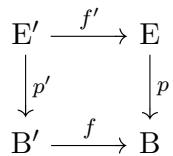
\includegraphics[keepaspectratio]{images/part002_b7191fdb.jpg}}

be a cartesian square. Suppose that E is a covering of B and that the space B' is connected and locally path-connected. Let b' be a point of B' and \(b = f(b')\) . For \((\mathrm{E}', p')\) to be a trivializable covering of B', it is necessary and sufficient that, for every point x of the fibre \(E_b\), the image of \(\pi_1(p, x)\) contain the image of \(\pi_1(f, b)\) .

This follows from prop. 1 and I, p. 81, cor. 5 of prop. 6.

\subsection{Operations of the Poincaré group and morphisms of coverings}

Let B be a connected and locally path-connected topological space and let b be a point of B.

Let E be a covering of B. Since the space B is assumed to be connected, the fibre \(E_{b}\) is nonempty if E is nonempty (I, p. 74, prop. 4). By assertion a) of theorem 1 of III, p. 305, the covering E is connected and nonempty if and only if the group \(\pi_{1}(B,b)\) acts transitively on \(E_{b}\) .

PROPOSITION 2. --- Let E and E' be coverings of B.

\begin{enumerate}
\def\labelenumi{\alph{enumi})}
\item
  Let \(f\colon\mathrm{E}\to\mathrm{E}^{\prime}\) be a B-morphism. The map \(f_{b}\colon\mathrm{E}_{b}\to\mathrm{E}_{b}^{\prime}\) deduced from \(f\) is compatible with the operations of \(\pi_{1}(\mathrm{B},b)\) on \(\mathrm{E}_{b}\) and \(\mathrm{E}_{b}^{\prime}\) respectively. It is bijective if and only if \(f\) is an isomorphism.
\item
  The map \(f\mapsto f_{b}\) is a bijection from the set \(\mathcal{C}_{\mathrm{B}}(\mathrm{E};\mathrm{E}^{\prime})\) of B-morphisms from E to \(\mathrm{E}^{\prime}\) onto the set \(\mathcal{F}_{\pi_1(\mathrm{B},b)}(\mathrm{E}_b;\mathrm{E}_b^{\prime})\) of \(\pi_1(\mathrm{B},b)\)-morphisms from \(\mathrm{E}_b\) to \(\mathrm{E}_b^{\prime}\) .
\end{enumerate}

If \(f\) is a B-morphism from E to \(\mathrm{E}'\) , the map \(f_b\colon \mathrm{E}_b\to \mathrm{E}_b'\) is a \(\pi_1(\mathrm{B},b)\) -morphism (cf. III, p. 305). Moreover, two B-morphisms from E to \(\mathrm{E}'\) which coincide on the fibre \(\mathrm{E}_b\) are equal (I, p. 80, cor. 3 of prop. 6).

Let \(\varphi\colon\mathrm{E}_{b}\to\mathrm{E}_{b}^{\prime}\) be a morphism of \(\pi_{1}(\mathrm{B},b)\)-sets; let us show that there exists a B-morphism \(f\) from E to \(\mathrm{E}^{\prime}\) such that \(f_{b}=\varphi\) . We may assume the spaces E and \(\mathrm{E}^{\prime}\) are connected and nonempty, so that \(\mathrm{E}_{b}\) and \(\mathrm{E}_{b}^{\prime}\) are homogeneous \(\pi_{1}(\mathrm{B},b)\)-sets. Let \(x\) be a point of \(\mathrm{E}_{b}\) ; its stabilizer G is the image of the map \(\pi_{1}(p,x)\) (III, p. 305, Theorem 1). Since the map \(\varphi\) is a \(\pi_{1}(\mathrm{B},b)\)-morphism, the group G fixes the point \(x^{\prime}=\varphi(x)\) of \(\mathrm{E}_{b}^{\prime}\) , hence is contained in the image of the map \(\pi_{1}(p^{\prime},x^{\prime})\) . By Prop. 1 of III, p. 308, there exists a B-morphism \(f\) from E to \(\mathrm{E}^{\prime}\) such that \(f(x)=x^{\prime}\) . The maps \(f_{b}\) and \(\varphi\) are \(\pi_{1}(\mathrm{B},b)\)-morphisms of the homogeneous \(\pi_{1}(\mathrm{B},b)\)-set \(\mathrm{E}_{b}\) to \(\mathrm{E}_{b}^{\prime}\) which coincide at the point \(x\) ; they are therefore equal.

If \(f\colon \mathrm{E}\to \mathrm{E}'\) is a B-isomorphism, the map \(f_{b}\colon \mathrm{E}_{b}\to \mathrm{E}_{b}^{\prime}\) is bijective. Conversely, suppose the map \(f_{b}\) is bijective and let \(g\colon \mathrm{E}^{\prime}\to \mathrm{E}\) be a B-morphism such that \(g_{b} = (f_{b})^{-1}\) . The B-morphism \(g\circ f\colon \mathrm{E}\to \mathrm{E}\) induces on \(\mathrm{E}_b\) the identity map; it therefore follows from the proposition that \(g \circ f = Id_{E}\) . Likewise, \(f \circ g = Id_{E'}\) , which proves that f is a B-isomorphism.

COROLLARY 1. --- The coverings E and E' are isomorphic if and only if the \(\pi_1(\mathrm{B},b)\) -sets \(\mathrm{E}_b\) and \(\mathrm{E}_b'\) are isomorphic.

COROLLARY 2. --- Let (E,p) and (E',p') be connected coverings of B. Let \(x\) be a point of \(E_{b}\) and \(x'\) a point of \(E'_{b}\) . For there to exist a B-morphism \(g\colon E\to E'\) such that \(g(x)=x'\), it is necessary and sufficient that \(p_{*}(\pi_{1}(E,x))\subset p'_{*}(\pi_{1}(E',x'))\). Such a morphism is then unique and is an isomorphism if and only if the subgroups \(p_{*}(\pi_{1}(E,x))\) and \(p'_{*}(\pi_{1}(E',x'))\) of \(\pi_{1}(B,b)\) are equal.

By III, p. 305, Theorem 1, the map from \(\pi_1(B,b)\) onto \(E_b\) defined by \(\gamma \mapsto x \cdot \gamma\) induces by passage to the quotient an isomorphism of the \(\pi_1(B,b)\)-set \(p_*(\pi_1(E,x)) \backslash \pi_1(B,b)\) onto \(E_b\) . Likewise, there exists a unique isomorphism of \(\pi_1(B,b)\)-sets from \(p'_{*}(\pi_1(E',x')) \backslash \pi_1(B,b)\) onto \(E_b'\) . By Proposition 2, there exists a B-morphism \(g\colon E\to E'\) such that \(g(x)=x'\) if and only if there exists a morphism of \(\pi_1(B,b)\)-sets from \(p_*(\pi_1(E,x)) \backslash \pi_1(B,b)\) onto \(p'_{*}(\pi_1(E',x')) \backslash \pi_1(B,b)\) sending the class \(p_*(\pi_1(E,x))\) to the class \(p'_{*}(\pi_1(E',x'))\) . Such a morphism exists if and only if one has \(p_*(\pi_1(E,x)) \subset p'_{*}(\pi_1(E',x'))\) . It is then unique, since the space E is assumed connected (I, p. 34, Cor. 2 of Prop. 11). It is an isomorphism if and only if the subgroups \(p_*(\pi_1(E,x))\) and \(p'_{*}(\pi_1(E',x'))\) of \(\pi_1(B,b)\) are equal.

COROLLARY 3. --- Let (E,p) be a connected covering of B and let x be a point of the fiber \(E_{b}\) . Let N denote the normalizer of \(p_{*}(\pi_{1}(E,x))\) in \(\pi_{1}(B,b)\) . For every element \(\gamma\) of N, there exists a unique B-automorphism g of E such that \(g(x) = x \cdot \gamma\) , and the map \(\gamma \mapsto g\) defines by passage to the quotient a group isomorphism from \(\mathrm{N}/p_{*}(\pi_{1}(\mathrm{E},x))\) onto \(\mathrm{Aut}_{\mathrm{B}}(\mathrm{E})\) .

Let \(\gamma \in \pi_1(\mathrm{B}, b)\) ; we have \(p_*(\pi_1(\mathrm{E}, x)) = \operatorname{Int}(\gamma)(p_*(\pi_1(\mathrm{E}, x \cdot \gamma)))\) (III, p. 305, Theorem 1, c)). By Corollary 2, for there to exist a B-automorphism \(g\) of E such that \(g(x) = x \cdot \gamma\) , it is necessary and sufficient that \(\gamma\) belongs to N. Such an isomorphism is then unique. Let us denote by \(\alpha: \mathrm{N} \to \mathrm{Aut}_{\mathrm{B}}(\mathrm{E})\) the map \(\gamma \mapsto g\) thus defined.

Let \(\gamma\) and \(\gamma'\) be two elements of N. Set \(g = \alpha(\gamma)\) , \(g' = \alpha(\gamma')\) ; we have \(g(g'(x)) = g(x \cdot \gamma') = g(x) \cdot \gamma' = (x \cdot \gamma) \cdot \gamma' = x \cdot (\gamma\gamma')\) by relations (4), III, p. 305 and (1), p. 304. Consequently, \(\alpha\) is a group homomorphism. For \(\alpha(\gamma) = \mathrm{Id}_{\mathrm{E}}\) , it is necessary and sufficient that one have \(x \cdot \gamma = x\) , by virtue of the uniqueness of \(\alpha(\gamma)\) , that is, \(\gamma \in p_*(\pi_1(E, x))\) (III, p. 305, Theorem 1, b)). Finally, if \(g\) is a B-automorphism of E, there exists a path \(c\) joining \(x\) to \(g(x)\) in E (which is path-connected), and one then has \(g(x) = x \cdot \gamma\) , where \(\gamma\) is the class of the path \(p \circ c\) . This proves that the homomorphism \(\alpha\) is surjective.

The group \(\mathrm{Aut}_{\mathrm{B}}(\mathrm{E})\) acts on the fibre \(\mathrm{E}_b\) and is identified with the group of automorphisms of the homogeneous \(\pi_1(\mathrm{B},b)\) -set (on the right) \(\mathrm{E}_b\) (cf. A, I, p. 56, prop. 5 and 6).

COROLLARY 4. --- Let (E, p) be a connected covering of B and let x be a point of the fibre \(E_{b}\) . For E to be a Galois covering of B, it is necessary and sufficient that \(p_{*}(\pi_{1}(E, x))\) be a distinguished subgroup of \(\pi_{1}(B, b)\) . The group \(\mathrm{Aut}_{\mathrm{B}}(\mathrm{E})\) is then isomorphic to the quotient group \(\pi_{1}(\mathrm{B}, b)/p_{*}(\pi_{1}(\mathrm{E}, x))\) .

If \(p_{*}(\pi_{1}(\mathrm{E},x))\) is a distinguished subgroup of \(\pi_1(\mathrm{B},b)\) , the group \(\mathrm{Aut}_{\mathrm{B}}(\mathrm{E})\) acts transitively on the fibre \(\mathrm{E}_b\) by Corollary 3, so that E is a Galois covering of B (I, p. 102, th. 2). The converse is assertion d) of Theorem 1 (III, p. 305). The last assertion follows from Corollary 3.

\subsection{Operations without local monodromy of the Poincaré groupoid}

Lemma 1. --- Let B be a locally arcwise connected topological space, let \(p \colon E \to B\) and \(p' \colon E' \to B\) be étale and separated maps satisfying the path lifting property (III, p. 302). Let \(g \colon E \to E'\) be a mapping such that \(p' \circ g = p\) . We assume that \(g\) is compatible with the canonical operations of the groupoid \(\varpi(B)\) on \(E\) and \(E'\) . Then, \(g\) is continuous.

Let c be a path in E; set \(c' = g \circ c\) and let us prove that the map \(c'\) is continuous. Let d denote the path \(p \circ c\) in B and, for every \(t \in I\) , denote by \(d_t\) the path \(s \mapsto d(st)\) . For all \(t \in I\) , we have \(c(t) = c(0) \cdot d_t\) (III, p. 304, remark 3), whence \(c'(t) = c'(0) \cdot d_t\) by the hypothesis made on g, which proves that \(c'\) is a path lifting the path d, by this same remark. This proves that the map g is continuous by arcs. Since the space E is locally arc-connected (III, p. 261, cor. 2), the map g is continuous (III, p. 269, corollary of prop. 13).

Let B be a topological space. Consider an operation \(\varphi = (\varphi_{a,b})_{(a,b)\in \mathrm{B}\times \mathrm{B}}\) of the groupoid \(\varpi (\mathrm{B})\) on a set E, with respect to a mapping \(p\colon \mathrm{E}\to \mathrm{B}\) . One says that \(\varpi (\mathrm{B})\) acts without monodromy on E (cf. II, p. 168) if for every \(b\in \mathrm{B}\) and every loop class \(\gamma \in \pi_1(\mathrm{B},b)\) the action of \(\gamma\) on the fiber \(\mathrm{E}_b\) is trivial. If B is path-connected, it suffices that this be the case for one point of B (loc. cit.). We shall say that the operation \(\varphi\) of the groupoid \(\varpi (\mathrm{B})\) is without local monodromy if every point of B has a neighborhood V such that \(\varpi (\mathrm{V})\) acts without monodromy on the set \(\mathrm{E_V} = p^{-1}(\mathrm{V})\) with respect to the map \(p_{\mathrm{V}} = p\mid p^{-1}(\mathrm{V})\) .

Remark. --- Let B be a locally path-connected topological space, and suppose that every point b of B has a neighborhood V such that the image of \(\pi_{1}(V,b)\) in \(\pi_{1}(B,b)\) is reduced to the identity element (cf. IV, p. 340, def. 2). Then, every operation of the groupoid \(\varpi(B)\) is without local monodromy.

Indeed, consider a set E, a mapping \(p \colon \mathrm{E} \to \mathrm{B}\) and an operation \(\varphi\) of the groupoid \(\varpi(\mathrm{B})\) on E with respect to \(p\) . Let \(a\) be a point of B, and let V be a neighborhood of \(a\) such that the image of \(\pi_1(\mathrm{V}, a)\) in \(\pi_1(\mathrm{B}, a)\) is reduced to the identity element. Let U be a path-connected neighborhood of \(a\) contained in V. Let \(b\) be a point of U and let \(\gamma \in \pi_1(\mathrm{U}, b)\) . Let \(\delta\) be the class of a path joining \(a\) to \(b\) in U. Then, \(\delta\gamma\delta^{-1}\) is the class of a loop at \(a\) in U; its image in \(\pi_1(\mathrm{B}, a)\) is therefore trivial. We thus have \(\varphi_{a,a}(\delta\gamma\delta^{-1}) = \mathrm{Id}_{\mathrm{E}_a}\) , whence \(\varphi_{b,b}(\gamma) = \mathrm{Id}_{\mathrm{E}_b}\) . This proves that the operation of \(\varpi(\mathrm{U})\) on the U-space \(\mathrm{E_U}\) is without monodromy. Consequently, the operation \(\varphi\) is without local monodromy.

PROPOSITION 3. --- Let B be a locally path-connected topological space and let E be a set equipped with an operation \(\varphi\) of the groupoid \(\varpi(B)\), without local monodromy, relative to a mapping \(p: E \to B\). There then exists on E a unique topology for which the following conditions are satisfied:

\begin{enumerate}
\def\labelenumi{(\roman{enumi})}
\item
  The set E equipped with this topology and with the map p is a covering of B;
\item
  The canonical action of \(\varpi(\mathrm{B})\) on this covering is identical to the action \(\varphi\) .
\end{enumerate}

The uniqueness of such a topology follows from lemma 1 of III, p. 312, where one takes for g the identity map of E. To prove its existence, one may moreover assume that B is connected and nonempty.

Suppose first that the operation \(\varphi = (\varphi_{a,b})_{(a,b)\in \mathrm{B}\times \mathrm{B}}\) of the groupoid \(\varpi (\mathrm{B})\) on the set E, relative to \(p\) , is without monodromy.

Let \(a\) be a point of B. For every point \(b \in \mathrm{B}\) , there exists a path \(c\) in B joining \(a\) to \(b\) . If \(\gamma \in \varpi_{a,b}(\mathrm{B})\) denotes the class of the path \(c\) , the bijection \(\varphi_{a,b}(\gamma) \colon \mathrm{E}_a \to \mathrm{E}_b\) is independent of the path \(c\) , since the operation is without monodromy; we denote by \(f_{a,b}\) this bijection. The map \(\Phi_a \colon \mathrm{B} \times \mathrm{E}_a \to \mathrm{E}\) defined by \((b,x) \mapsto f_{a,b}(x)\) is a bijection; the inverse bijection maps \(x \in \mathrm{E}\) to the pair \((p(x), f_{p(x),a}(x))\) . Endow the set \(\mathrm{E}_a\) with the discrete topology, so that the B-space \(\mathrm{B} \times \mathrm{E}_a\) is a trivial covering of B. By transport of structure, the bijection \(\Phi_a\) endows E with a topology making it a covering of B.

Let us prove that the canonical operation of \(\varpi(\mathrm{B})\) on E is identical to the operation \(\varphi\) . Let \(x\) be a point of \(\mathrm{E}_a\) and \(b\) a point of B. Let \(c\) be a path in B joining the point \(a\) to the point \(b\) ; the map \(t \mapsto \Phi_a(c(t), x)\) is then a path in E joining the point \(x\) to the point \(\Phi_a(b, x) = f_{a,b}(x)\) . If \(\gamma \in \varpi_{a,b}(\mathrm{B})\) denotes the class of the path \(c\) , we thus have \(x \cdot \gamma = f_{a,b}(x)\) . This shows that the canonical action of \(\varpi(\mathrm{B})\) on the covering E and the operation \(\varphi\) coincide on the classes of paths of origin \(a\) . Since these classes generate the groupoid \(\varpi(\mathrm{B})\) , the two operations are equal.

Now let us treat the general case. Let \(\mathcal{B}\) be the set of open subsets V of E such that \(\varpi(\mathrm{V})\) acts without monodromy on \(p^{-1}(\mathrm{V})\) . By hypothesis, the elements of \(\mathcal{B}\) cover B. By the preceding, there exists for every \(\mathrm{V} \in \mathcal{B}\) a unique topology on the set \(p^{-1}(\mathrm{V})\) such that \((p^{-1}(\mathrm{V}), p_{\mathrm{V}})\) makes it a covering of V and such that the canonical action of \(\varpi(\mathrm{V})\) on this covering coincides with the action induced by \(\varphi\) .

Let V and \(V' \in \mathcal{B}\) . The topology of \(p^{-1}(V \cap V')\) induced by the topology of \(p^{-1}(V)\) (resp. of \(p^{-1}(V')\) ) defined above indeed makes a covering of \(V \cap V'\) on which the canonical operation of \(\varpi(V \cap V')\) is induced by the operation \(\varphi\) . These topologies therefore coincide with that of \(p^{-1}(V \cap V')\) . There then exists a unique topology on E inducing on each \(p^{-1}(V)\) the topology previously defined (cf. I, §2, p. 16).

When E is equipped with this topology, the map p is continuous and the B-space E is a covering. The canonical action of \(\varpi(\mathrm{B})\) on this covering coincides with the operation \(\varphi\) on the classes of paths whose image is contained in one of the open sets of \(\mathcal{B}\) . By Lemma 4 of

III, p. 272, these classes generate the groupoid \(\varpi(B)\) . It follows that these two operations are equal (II, p. 167).

COROLLARY. --- Let B be a connected and locally arcwise connected topological space, let (E,p) be a B-space whose projection p is étale, separated, and has the path lifting property. If the canonical operation of \(\varpi(\mathrm{B})\) on the set E, relative to p, is without local monodromy, then E is a covering of B.

Endow E with the canonical action of \(\varpi(B)\) defined by the lifting of paths (III, p. 303, no. 3). There exists a topology on E for which conditions (i) and (ii) of Prop. 3 are satisfied. This topology coincides with the given topology on E by Lemma 1 of III, p. 312.

\subsection{Admissible topology of Poincaré groups}

Let B be a topological space and let \(a\) be a point of B. We say that a subgroup H of \(\pi_1(B, a)\) is admissible if every point \(b\) of B has a neighborhood V such that \(\gamma i_*(\delta)\gamma^{-1} \in \mathrm{H}\) for every \(\gamma \in \varpi_{a,b}(\mathrm{B})\) and every \(\delta \in \pi_1(V, b)\) , where \(i: V \to B\) is the canonical injection. If H is a normal subgroup of \(\pi_1(B, a)\) , it suffices, for H to be admissible, that this condition be verified for one path class \(\gamma \in \varpi_{a,b}(\mathrm{B})\) .

Proposition 4. — There exists a unique topology on \(\pi_1(B, a)\) compatible with its group structure, for which the admissible distinguished subgroups of \(\pi_1(B, a)\) form a fundamental system of neighborhoods of the identity element. For this topology, the open subgroups are exactly the admissible subgroups.

The following facts result from the definition of an admissible subgroup:

\begin{enumerate}
\def\labelenumi{\alph{enumi})}
\item
  The group \(\pi_1(B, a)\) is admissible;
\item
  A subgroup containing an admissible subgroup is admissible;
\item
  The intersection of a finite family of admissible subgroups is admissible.
\item
  For every admissible subgroup H of \(\pi_{1}(B,a)\) the intersection of the subgroups \(\gamma H\gamma^{-1}\) , when \(\gamma\) runs through \(\pi_{1}(B,a)\) , is admissible.
\end{enumerate}

In particular, the set of admissible normal subgroups is a filter base consisting of subgroups of \(\pi_1(B,a)\) satisfying the axiom (GV \(_{\text{III}}'\) ) of III, p. 4, whence the first part of the proposition according to TG, III, p. 5, example. The second part is then immediate (cf. TG, III, p. 7, corollary of prop. 4).

The topology on the group \(\pi_{1}(B,a)\) characterized in Proposition 4 is called the admissible topology.

Remarks. --- 1) If B \(_{0}\) denotes the arcwise connected component of \(a\) in B, the canonical isomorphism \(\pi_{1}(B_{0}, a) \to \pi_{1}(B, a)\) is an isomorphism of topological groups when these groups are equipped with the admissible topology.

\begin{enumerate}
\def\labelenumi{\arabic{enumi})}
\setcounter{enumi}{1}
\item
  Let B be a topological space. Let \(b\) and \(b'\) be points of B belonging to the same path-connected component, and let \(\gamma\) be an element of \(\varpi_{b,b'}(B)\) . It follows from the definition of an admissible subgroup that, for every admissible subgroup H of \(\pi_1(B,b')\) , the subgroup \(\gamma H\gamma^{-1}\) of \(\pi_1(B,b)\) is admissible. Consequently, the isomorphism \(u_\gamma \colon \delta \mapsto \gamma \delta \gamma^{-1}\) of \(\pi_1(B,b')\) onto \(\pi_1(B,b)\) (cf. III, p. 292) is a homeomorphism when these groups are equipped with the admissible topologies.
\item
  Let A and B be topological spaces, let \(a\) be a point of A and let \(f\colon\mathrm{A}\to\mathrm{B}\) be a continuous map. Set \(b=f(a)\) . If H is an admissible subgroup of \(\pi_{1}(\mathrm{B},b)\) , its inverse image under the homomorphism \(\pi_{1}(f,a)\) is an admissible subgroup of \(\pi_{1}(\mathrm{A},a)\) . Consequently, the group homomorphism \(\pi_{1}(f,a)\colon\pi_{1}(\mathrm{A},a)\to\pi_{1}(\mathrm{B},b)\) is continuous, when these groups are equipped with the admissible topology.
\end{enumerate}

PROPOSITION 5. --- Let B be a locally path-connected topological space and let a be a point of B. For a subgroup H of \(\pi_1(\mathrm{B},a)\) to be admissible, it is necessary and sufficient that there exist a covering (E,p) of B and a point \(x\in \mathrm{E}_a\) such that \(\mathrm{H} = p_{*}(\pi_{1}(\mathrm{E},x))\) .

Let \((\mathrm{E},p)\) be a covering of B and let x be a point of \(E_{a}\) ; set \(\mathrm{H}=p_{*}(\pi_{1}(\mathrm{E},x))\) and let us show that it is an admissible subgroup of \(\pi_{1}(\mathrm{B},a)\) . Let b be a point of B and let V be a neighborhood of b such that \(\mathrm{E}_{\mathrm{V}}=(p^{-1}(\mathrm{V}),p_{\mathrm{V}})\) is a trivializable covering of V. Let \(\gamma\in\varpi_{a,b}(\mathrm{B})\) ; we shall prove that for every element \(\delta\in\pi_{1}(\mathrm{V},b)\) , the path class \(\gamma\delta\gamma^{-1}\) belongs to H.

By III, p. 301, prop. 3, there exists a unique strict homotopy class \(\gamma'\) of a path with origin \(x\) in E such that \(p_*(\gamma') = \gamma\) . Let \(y\) be the terminal point of \(\gamma'\) ; we have \(p(y) = b\) (III, p. 302, prop. 4). Let then \(\delta'\) be the unique path class with origin \(y\) in E such that \(p_*(\delta') = \delta\) . Since \(\mathrm{E_V}\) is trivializable, \(\delta'\) is the class of a loop at \(y\) . Then, \(\gamma'\delta'(\gamma')^{-1}\) is the class of a loop at \(a\) in E whose image under \(p_*\) is the class \(\gamma\delta\gamma^{-1}\) , which is what had to be proved.

Conversely, let H be an admissible subgroup of \(\pi_1(B, a)\) . Let \(\lambda_a(B)\) be the quotient of the space \(\Lambda_a(B)\) of paths with origin \(a\) for the strict homotopy relation; since two strictly homotopic paths have the same endpoint, the endpoint map \(e: \Lambda_a(B) \to B\) defines by passage to the quotient a map \(\varepsilon: \lambda_a(B) \to B\) . The composition of path classes endows the set \(\lambda_a(B)\) with a left action of the group \(\pi_1(B, a)\) . Equip it with the action of the group H obtained by restriction, and denote by \(H\backslash\lambda_a(B)\) the set of its orbits.

The map \(\varepsilon\colon\lambda_{a}(B)\to B\) induces, by passing to the quotient, a map \(q\colon H\backslash\lambda_{a}(B)\to B\) . The composition of path classes endows the set \(H\backslash\lambda_a(B)\) with a right action of the groupoid \(\varpi(B)\) with respect to the map \(q\) .

This operation has no local monodromy. Indeed, let \(b\) be a point of B, and let V be a neighborhood of \(b\) such that \(\gamma i_{*}(\pi_{1}(V,b))\gamma^{-1}\subset H\) for every path class \(\gamma\) connecting \(a\) to \(b\) in B, where \(i\) denotes the inclusion of V into B. Since B is locally path-connected, one may further assume that V is path-connected. Let \(c\in V\) , let \(\delta\) be the class in \(\pi_1(B,c)\) of a loop at \(c\) contained in V, and let \(\delta'\) be an element of \(\lambda_a(B)\) such that \(\varepsilon (\delta ') = c\) . Let \(\delta''\) be an element of \(\varpi_{c,b}(V)\) and let us set \(\gamma = \delta '\delta ''\) . By definition of V, the element \(\delta '\delta (\delta ')^{-1} = \gamma ((\delta '')^{-1}\delta \delta '')\gamma^{-1}\) of \(\pi_1(B,a)\) belongs to H. Then, \(\mathrm{H}\delta^{\prime}\cdot \delta = \mathrm{H}\delta^{\prime}\) ; this proves that \(\pi_1(V,c)\) acts trivially on the set \(q^{-1}(c)\) .

By III, p. 313, prop. 3, there exists a unique topology on \(\mathrm{H}\backslash\lambda_{a}(\mathrm{B})\) for which \(q\) is continuous and the B-space \((\mathrm{H}\backslash\lambda_{a}(\mathrm{B}),q)\) is a covering such that the canonical action of \(\varpi(\mathrm{B})\) on this covering is the action defined above. By assertion b) of Theorem 1 of III, p. 305, the group \(q_{*}(\pi_{1}(\mathrm{H}\backslash\lambda_{a}(\mathrm{B}),\mathrm{H}))\) is equal to H.

We will say that an operation of the group \(\pi_1(B, b)\) on a set X is admissible if the kernel of the canonical map \(\pi_1(B, b) \to \mathfrak{S}_{\mathrm{X}}\) is an open subgroup of \(\pi_1(B, b)\) . This amounts to saying that the homomorphism \(\pi_1(B, b) \to \mathfrak{S}_{\mathrm{X}}\) is continuous if the group \(\mathfrak{S}_{\mathrm{X}}\) is equipped with the discrete topology. The map \(\pi_1(B, b) \times X \to X\) is then continuous, when X is endowed with the discrete topology. Conversely, consider a continuous action of \(\pi_{1}(B,b)\) on a discrete space X. Let x be a point of X; its stabilizer is an open subgroup H of \(\pi_{1}(B,b)\) by hypothesis. For \(\gamma\in\pi_{1}(B,b)\) the fixator of \(\gamma\cdot x\) is the subgroup \(\gamma H\gamma^{-1}\) , so that the subgroup of \(\pi_{1}(B,b)\) fixing each element of the orbit of x is the intersection of the subgroups \(\gamma H\gamma^{-1}\) , for \(\gamma\) running through \(\pi_{1}(B,b)\) . It is an open subgroup because the distinguished open subgroups of \(\pi_{1}(B,b)\) form a basis for its topology (III, p. 315, prop. 4). This implies that a continuous action of \(\pi_{1}(B,b)\) on a discrete space X is admissible if it is transitive or, more generally, if the set of orbits of the elements of X is finite.

For any discrete group \(G\), any principal \(G\)-covering \(E\) over \(B\), and any point \(x \in E_{b}\) , recall that the map \(h_{(\mathrm{E},x)}\) from \(\pi_{1}(\mathrm{B},b)\) to G which, to \(\gamma \in \pi_{1}(\mathrm{B},b)\) , associates the unique element \(g \in G\) such that \(x \cdot g = x \cdot \gamma^{-1}\) is a group homomorphism (III, p. 306, prop. 5).

PROPOSITION 6. --- Let B be a topological space and let b be a point of B. Endow the group \(\pi_1(B, b)\) with the admissible topology.

\begin{enumerate}
\def\labelenumi{\alph{enumi})}
\item
  For any discrete group G, any principal covering E of B with group G, and any \(x \in E_{b}\) , the homomorphism \(h_{(E,x)}\) is a continuous homomorphism of topological groups.
\item
  For every covering E of B, the canonical action of \(\pi_{1}(B,b)\) on the fiber \(E_{b}\) is admissible.
\end{enumerate}

It suffices to prove the second assertion. Let K be the set of elements \(k \in \pi_{1}(B, b)\) such that \(x \cdot k = x\) for all \(x \in E_{b}\) . Let us prove that K is an admissible subgroup of \(\pi_{1}(B, b)\) .

Let \(b'\) be a point of B and let \(V'\) be a neighborhood of \(b'\) in B above which the covering E is trivializable. Let \(\gamma\) be the class of a path c connecting \(b\) to \(b'\) in B and let \(c'\) be the unique path starting at x in E that lifts c. For all \(\delta \in \pi_1(V', b')\) and every \(x' \in E_{b'}\) , we have \(x' \cdot \delta = x'\) . Consequently, for \(x \in E_b\) and \(\delta \in \pi_1(V', b')\) , we have

\[
x \cdot \gamma \delta \gamma^ {- 1} = ((x \cdot \gamma) \cdot \delta) \cdot \gamma^ {- 1} = (x \cdot \gamma) \cdot \gamma^ {- 1} = x,
\]

so that \(\gamma\delta\gamma^{-1}\) belongs to K. In other words, K is an admissible subgroup, whence the proposition.

PROPOSITION 7. --- Let B be a connected and locally path-connected topological space, and let b be a point of B. Endow the group \(\pi_1(B, b)\) with the admissible topology.

\begin{enumerate}
\def\labelenumi{\alph{enumi})}
\item
  Let G be a discrete topological group. For every continuous homomorphism \(f\colon \pi_{1}(\mathrm{B},b)\to \mathrm{G}\) , there exists a principal covering E of B with group G, and a point \(x\) of \(\mathrm{E}_{b}\) such that \(h_{(\mathrm{E},x)} = f\) .
\item
  For every discrete topological space F equipped with an admissible right action of the group \(\pi_{1}(B,b)\), there exists a covering E of B such that the \(\pi_{1}(B,b)\)-sets F and \(E_{b}\) are isomorphic.
\end{enumerate}

Let us prove \(a\) ). Let \(f\) be a continuous homomorphism of \(\pi_1(B, b)\) into a discrete group G. Its kernel is an open normal subgroup K of \(\pi_1(B, b)\) ; denote by H the group \(\pi_1(B, b)/K\) and \(\overline{f} \colon H \to G\) the group homomorphism induced by \(f\) by passing to the quotient. By III, p. 316, prop. 5, there exists a connected covering E' of B such that the subgroup K is the stabilizer of every point of the fibre \(E'_{b}\) ; the covering E' is principal with group H = \(\pi_1(B, b)/K\) . Let \(x'\) be a point of \(E'_{b}\) ; the homomorphism \(h_{(E', x')} \colon \pi_1(B, b) \to H\) is surjective with kernel K (III, p. 306, prop. 5). Let then \(\varphi \colon H \to G\) be the unique homomorphism of groups such that \(\varphi \circ h_{(E', x')} = f\) . The associated covering \(E = E' \times^{H} G\) of B is principal with group G, and one has \(h_{(E, x)} = \varphi \circ h_{(E', x')} = f\) (III, p. 307, example 2). This proves assertion \(a\) ).

Let us prove \(b\) ). Let F be a set equipped with an admissible right action of the group \(\pi_1(B,b)\) . Denote by \(f: \pi_1(B,b) \to \mathfrak{S}_{\mathrm{F}}\) this action and endow the group \(\mathfrak{S}_{\mathrm{F}}\) with the discrete topology. By \(a\) ), there exists a principal covering E of B with group \(\mathfrak{S}_{\mathrm{F}}\) , and a point \(x \in \mathrm{E}\) such that the homomorphism \(h_{(\mathrm{E},x)}\) is equal to \(f\) . The canonical action of the group \(\pi_1(B,b)\) on the fibre over \(b\) of the associated covering \(\mathrm{E} \times^{\mathfrak{S}_{\mathrm{F}}} \mathrm{F}\) of B is identified with the action of \(\pi_1(B,b)\) on F (III, p. 306, example 1).

Remarks. --- 4) The admissible topology on \(\pi_1(B, b)\) is the coarsest topology for which the action of \(\pi_1(B, b)\) on \(E_b\) is continuous for every connected covering E of B (prop. 6 of III, p. 318 and prop. 7 of III, p. 318). If E is a connected covering of B and \(x\) a point of the fibre \(E_b\) , the map \(c' \mapsto c'(1)\) of \(\Lambda_x(E)\) in E is continuous. Consequently, the map \(c \mapsto x \cdot c\) of \(\Lambda_b(B)\) in E is continuous (III, p. 302, cor. 2 of prop. 3). By restriction to \(\Omega_b(B)\) and passage to the quotient, one deduces that the map \(\gamma \mapsto x \cdot \gamma\) is continuous when one endows the group \(\pi_1(B, b)\) with the quotient topology of \(\Omega_b(B)\) . The admissible topology on \(\pi_{1}(B,b)\) is therefore coarser than the quotient topology of the topology of compact convergence. It can be strictly coarser (III, p. 337, exerc. 7).

\begin{enumerate}
\def\labelenumi{\arabic{enumi})}
\setcounter{enumi}{4}
\tightlist
\item
  Let B be a connected and locally path-connected topological space, let \(a\) be a point of B and let H be a subgroup of \(\pi_1(B,a)\) . By the preceding remark, if H is admissible, it is also open for the quotient topology of the topology of compact convergence. Conversely, suppose that H is a distinguished subgroup of \(\pi_1(B,a)\) which is open for the quotient topology of the topology of compact convergence. Let \(x\) be a point of B and let \(\gamma \in \varpi_{a,x}(B)\) . The subgroup \(\gamma^{-1}H\gamma\) of \(\pi_1(B,x)\) is still open for the quotient topology of the topology of compact convergence (III, p. 293, remark 3). There therefore exists a neighborhood V of \(x\) in B such that \(\gamma^{-1}H\gamma\) contains the class of every loop at \(x\) whose image is contained in V. We thus have \(\gamma \pi_1(V,x)\gamma^{-1} \subset H\) ; since H is distinguished, this implies that H is an admissible subgroup of \(\pi_1(B,a)\) .
\end{enumerate}

\exerciseshdr{Exercises}

\exercisegroup

\begin{enumerate}
\def\labelenumi{\arabic{enumi})}
\tightlist
\item
  For every \(\theta \in \mathbf{R}\) , let \(C_{\theta}\) be the segment of the plane with endpoints \((0,0)\) and \((\cos(2\pi\theta), \sin(2\pi\theta))\) ; set
\end{enumerate}

\[
\mathrm{C} = \bigcup_ {\theta \in \mathbf {Q} \cap [ 1 / 6, 1 / 4 ]} \mathrm{C} _ {\theta}.
\]

\begin{enumerate}
\def\labelenumi{\alph{enumi})}
\item
  The space C is contractible at 0, but at no other point.
\item
  Let D be the union of the translates \((0, n) + \mathrm{C}\) of C, for \(n \in Z\) . Show that the space D is homotopy equivalent to a point but is not contractible at any of its points.
\end{enumerate}

\begin{enumerate}
\def\labelenumi{\arabic{enumi})}
\setcounter{enumi}{1}
\tightlist
\item
  Let B be a subset of \(\mathbf{R}^{n}\) , let \(a\) be a point interior to B; denote by S the boundary of B. Suppose that B is star-shaped at \(a\) and that every half-line with origin \(a\) meets S in a unique point. Let \(f\colon\mathbf{R}_{+}^{*}\times\mathrm{S}\to\mathbf{R}^{n}-\{a\}\) be the map defined by \(f(t,y)=ty+(1-t)a\) . Prove that \(f\) is a homeomorphism such that \(f([0,1]\times\mathrm{S})=\mathrm{B}-\{a\}\) and \(f(\{1\}\times\mathrm{S})=\mathrm{S}\) .
\end{enumerate}

This result applies in particular when B is a convex, closed, and bounded subset of \(R^{n}\) and a is a point adherent to B (cf. I, p. 123, prop. 2 and EVT, II, p. 15, prop. 16).

\begin{enumerate}
\def\labelenumi{\arabic{enumi})}
\setcounter{enumi}{2}
\item
  Let X be the topological space obtained from the space R by contracting the subset Q (III, p. 252, def. 10). The canonical surjection \(p: R \rightarrow X\) is neither open nor closed.
\item
  Let X be the interval \([-1,1]\) of R and let A = X - \{0\}. The canonical map of X onto X/A is a homotopy equivalence but there does not exist a homotopy σ with origin \(\mathrm{Id}_{X}\) satisfying the hypotheses of prop. 10 of III, p. 252.
\item
  Let A be the closure in \(\mathbf{R}\) of the set of real numbers of the form \(1/n\) , where \(n\) runs through the set of integers \(\geqslant 1\) . Let \(i\) be the canonical injection of A into \(\mathbf{R}\) . The canonical map of \(\mathrm{Côn}(i)\) onto \(\mathbf{R}/\mathrm{A}\) is not a homotopy equivalence.
\item
  Let X be a metrizable topological space of countable type. We say that X is an absolute retract\(^{(1)}\) if for every metrizable topological space of countable type Y and every closed subset B of Y, every continuous map \(f: B \to X\) extends to a continuous map from Y into X.
\end{enumerate}

\begin{enumerate}
\def\labelenumi{\alph{enumi})}
\item
  Let X be a metrizable topological space of countable type. For X to be an absolute retract, it is necessary and sufficient that, for every metrizable space of countable type Y and every continuous, injective, and closed map f from X into Y, there exists a continuous map \(g: Y \to X\) such that \(g \circ f = Id_{X}\) .
\item
  Show that the spaces I and R are absolute retracts.
\item
  Show that the product space of a countable family of absolute retracts is an absolute retract.
\item
  Let X be an absolute retract, let A be a subspace of X which is a retract of X. Show that A is an absolute retract.
\end{enumerate}

\begin{enumerate}
\def\labelenumi{\arabic{enumi})}
\setcounter{enumi}{6}
\tightlist
\item
  Let X be a metrizable topological space of countable type. We say that X is an absolute neighborhood retract if for every metrizable topological space of countable type Y and every closed subset B of Y, every continuous map \(f: B \rightarrow X\) extends to a continuous map from a neighborhood of B into X.
\end{enumerate}

\begin{enumerate}
\def\labelenumi{\alph{enumi})}
\item
  Let X be a metrizable topological space of countable type. For X to be an absolute neighborhood retract, it is necessary and sufficient that for every metrizable space of countable type Y and every continuous, injective, and closed map f from X into Y, there exists a neighborhood U of \(f(\mathrm{X})\) and a continuous map \(g: U \to X\) such that \(g \circ f = Id_{X}\) .
\item
  Let X be an absolute neighborhood retract and let A be a subset of X. If A has a neighborhood U of which it is a retract, then A is an absolute neighborhood retract. In particular, every open subset of X and every retract of X is an absolute neighborhood retract.
\item
  Show that the product space of a finite family of absolute neighborhood retracts is an absolute neighborhood retract.
\end{enumerate}

d) Show that the sphere \(\mathbf{S}_n\) is an absolute neighborhood retract.

\begin{enumerate}
\def\labelenumi{\alph{enumi})}
\setcounter{enumi}{4}
\item
  Let X be a metrizable topological space of countable type, let \(A_{1}\) and \(A_{2}\) be closed subsets of X such that \(X = A_{1} \cup A_{2}\) . We assume that \(A_{1} \cap A_{2}\) is an absolute neighborhood retract. For X to be an absolute neighborhood retract, it is necessary and sufficient that the same be true of \(A_{1}\) and of \(A_{2}\) .
\item
  Let X be a metrizable topological space of countable type. If X is the union of two open subsets which are absolute neighborhood retracts, then X is an absolute neighborhood retract.
\item
  Let X be a metrizable topological space of countable type such that every point has a neighborhood which is an absolute neighborhood retract. Show that X is an absolute neighborhood retract.
\end{enumerate}

\begin{enumerate}
\def\labelenumi{\arabic{enumi})}
\setcounter{enumi}{7}
\tightlist
\item
  Let X be a metrizable topological space; let d be a metric defining its topology. Let \(\mathcal{C}_{b}(\mathrm{X};\mathbf{R})\) be the vector space of real-valued functions on X that are continuous and bounded; we equip it with the norm defined by \(\|f\| = \sup_{x \in X} |f(x)|\) for \(f \in \mathcal{C}_{b}(\mathrm{X};\mathbf{R})\) .
\end{enumerate}

\begin{enumerate}
\def\labelenumi{\alph{enumi})}
\item
  One defines a map \(j\colon X \to \mathcal{C}_{b}(X; \mathbf{R})\) by setting \(j(x)\colon y \mapsto d(x, y)/(1 + d(x, y))\) . Prove that the map j induces a homeomorphism from X onto its image.
\item
  Let V be the intersection of all convex subsets of \(\mathcal{C}_{b}(\mathrm{X};\mathbf{R})\) that contain \(j(\mathrm{X})\) . Prove that \(j(\mathrm{X})\) is closed in V.
\item
  Let X be a metrizable space of countable type. Prove that there exists a convex subset Z of \(I^{N}\) such that X is homeomorphic to a closed subset of Z.
\end{enumerate}

\begin{enumerate}
\def\labelenumi{\arabic{enumi})}
\setcounter{enumi}{8}
\tightlist
\item
  If X and Y are topological spaces and U is a set of subsets of X, we say that maps \(f, g: Y \to X\) are U-close if for every point \(y \in Y\) , there exists \(U \in U\) such that \(f(y)\) and \(g(y)\) belong to U; we say that a homotopy \(\sigma: Y \times I \to X\) is U-small if for every point \(y \in Y\) , there exists \(U \in U\) such that \(\sigma(y, t) \in U\) for all \(t \in I\) .
\end{enumerate}

Let X be a closed subspace of a convex subset Z of \(I^{N}\) (cf. Exercise 8); we assume that X is an absolute neighborhood retract.

\begin{enumerate}
\def\labelenumi{\alph{enumi})}
\item
  Let U be a cover of X by open subsets of \(I^{N}\) . Prove that there exists a family V of open and convex subsets of \(I^{N}\) such that, for every open set \(v \in V\) , there exists an open set \(u \in U\) such that \(v \cap X \subset u\) , and a continuous retraction r of the canonical injection of X into the union V of the family V.
\item
  Let Y be a topological space and let B be a closed subspace of Y. Let \(f, g: \mathrm{Y} \to \mathrm{X}\) be continuous maps that are \(\mathcal{V}\)-close, and let \(\sigma: \mathrm{B} \times \mathbf{I} \to \mathrm{X}\) be a homotopy \(\mathcal{V}\)-small whose origin is equal to \(f|_{\mathrm{B}}\) .
\end{enumerate}

Prove that there exists a neighborhood W of B in Y and a continuous map h from the subspace \((\mathbf{Y} \times \{0,1\}) \cup (\mathbf{W} \times \mathbf{I})\) of \(Y \times I\) into X such that \(h(y,0) = f(y)\) and \(h(y,1) = g(y)\) for all \(y \in Y\) , and \(h(y,t) = \sigma(y,t)\) for all \(y \in B\) and every \(t \in I\) . Prove that there exists a neighborhood \(W'\) of B contained in W such that \(h \mid W' \times I\) is a \(\mathcal{V}\)-small homotopy.

\begin{enumerate}
\def\labelenumi{\alph{enumi})}
\setcounter{enumi}{2}
\tightlist
\item
  Let \(u \colon \mathrm{Y} \to \mathbf{I}\) be a continuous map such that \(u(y) = 1\) for \(y \in \mathrm{B}\) and \(u(y) = 0\) in a neighborhood of \(\mathrm{Y} - \mathrm{W}\) ; set
\end{enumerate}

\[
h ^ {\prime} (y, t) = \left\{ \begin{array}{l l} (1 - u (y)) ((1 - t) f (y) + t g (y)) + u (y) h (y, t) & \text { if } y \in \mathrm{V} \\ (1 - t) f (y) + t g (y) & \text { otherwise. } \end{array} \right.
\]

Prove that \(h'\) is continuous and that its image is contained in V.

\(d)\) Deduce that there exists a homotopy \(\widetilde{\sigma}\colon\mathbf{Y}\times\mathbf{I}\to\mathbf{X}\) with source \(f\) , with endpoint \(g\) , which is \(\mathcal{U}\) -small.

\begin{enumerate}
\def\labelenumi{\arabic{enumi})}
\setcounter{enumi}{9}
\tightlist
\item
  Let X be a topological space. Suppose that there exists an open cover U of X such that for every topological space Y and every closed subspace B of Y, two maps \(f_{0}, f_{1}\) from Y to X which are U-close are homotopic if there exists a U-small homotopy connecting \(f_{0} \mid B\) to \(f_{1} \mid B\) .
\end{enumerate}

\begin{enumerate}
\def\labelenumi{\alph{enumi})}
\item
  Let a be a point of X and let U be an element of U such that \(a \in U\) . Prove that there exists a homotopy \(\sigma: U \times I \to X\) such that \(\sigma(x,0) = a\) , \(\sigma(x,1) = x\) and \(\sigma(a,t) = a\) for all \(x \in X\) and every \(t \in I\) .
\item
  Let V be an open neighborhood of a such that \(\sigma(\mathrm{V} \times \mathbf{I}) \subset \mathrm{U}\) . Prove that V is an absolute neighborhood retract.
\item
  Prove that X is an absolute neighborhood retract.
\end{enumerate}

\begin{enumerate}
\def\labelenumi{\arabic{enumi})}
\setcounter{enumi}{10}
\tightlist
\item
  Let X be an absolute neighborhood retract.
\end{enumerate}

\begin{enumerate}
\def\labelenumi{\alph{enumi})}
\item
  Prove that X is "semi-locally contractible", that is, every point x of X has a neighborhood V such that the canonical injection of (V, x) into X is strictly homotopic to the constant map with image x. (Use Exercise 9.)
\item
  Let A be a compact topological space. Prove that the path-connected components of the space \(\mathcal{C}_{c}(\mathrm{A};\mathrm{X})\) are open.
\item
  Prove that X is locally path-connected.
\end{enumerate}

\begin{enumerate}
\def\labelenumi{\arabic{enumi})}
\setcounter{enumi}{11}
\tightlist
\item
  Let X and Y be topological spaces; one says that the homotopy extension property holds for continuous maps with target X and source Y if for every continuous map F: \(Y \rightarrow X\) , every closed subspace B of Y, and every homotopy \(\sigma\colon\mathrm{B}\times\mathbf{I}\to\mathrm{X}\) with origin F \textbar{} B, there exists a homotopy \(\widetilde{\sigma}\colon\mathrm{Y}\times\mathbf{I}\to\mathrm{X}\) with origin F which extends \(\sigma\) .
\end{enumerate}

\begin{enumerate}
\def\labelenumi{\alph{enumi})}
\item
  Let X be a topological space which is an absolute neighborhood retract. Prove that the homotopy extension property holds for continuous maps with target X and source a metrizable space of countable type.
\item
  Prove the equivalence of the following two properties:
\end{enumerate}

\begin{enumerate}
\def\labelenumi{(\roman{enumi})}
\item
  The space X is an absolute neighborhood retract;
\item
  Every point of X has a neighborhood V such that for every metrizable topological space Y of countable type, every closed subspace B of Y, and every continuous map from B to V extends to a continuous map from Y to X.
\end{enumerate}

\begin{enumerate}
\def\labelenumi{\alph{enumi})}
\setcounter{enumi}{2}
\item
  Suppose that X is semi-locally contractible (cf. Exercise 9) and that the homotopy extension property holds for continuous maps with target X. Prove that X is an absolute neighborhood retract. \(^{(2)}\)
\item
  Prove that the space X = Q is not an absolute neighborhood retract but that the homotopy extension property holds for continuous maps with target X.
\end{enumerate}

\begin{enumerate}
\def\labelenumi{\arabic{enumi})}
\setcounter{enumi}{12}
\item
  Let X be a topological space which is an absolute neighborhood retract. Let A be a subset of X such that the canonical injection of A into X is a homotopy equivalence and a cofibration. There exists a contraction of X onto A.
\item
  Let X be the topological space I and set A = \{0,1\}. Prove that there exists a homotopy connecting the identity map of X to a constant map but that the canonical map X → X/A is not a homotopy equivalence.
\item
  Let X be the subspace of \([0,1]\times[0,1]\) consisting of the pairs \((x,y)\) such that \(x\in\{0,1\}\) , or \(y\in\{0,1\}\) , or \(x\neq0\) and \(1/x\in N\) . Let A = \(\{0\}\times[0,1]\) . Show that the canonical map from X onto X/A is not a homotopy equivalence, although A is contractible.
\item
  Let X and Y be topological spaces, and let \(f: X \to Y\) be a continuous map. Let \(\varphi: C(X) \to \text{Côn}(f)\) be the canonical map. Show that the spaces \(Y/f(X)\) and \(\text{Côn}(f)/\varphi(C(X))\) are homeomorphic.
\item
  Let X be a topological space and let A be a subspace of X. Denote by \(i\colon A \to X\) and \(j\colon \operatorname{Cyl}(i) \to X \times I\) the canonical injections.
\end{enumerate}

\begin{enumerate}
\def\labelenumi{\alph{enumi})}
\item
  Suppose that X = R and \(A = ]0, 1[\); show that the map j is not strict.
\item
  Suppose that every point of X has a countable base of closed neighborhoods. For the map j to be strict, it is necessary and sufficient that A be closed.
\item
  Suppose that A is the Alexandroff half-line (TG, IV, p. 49, exerc. 12) and that X is its Alexandroff compactification. Show that the map j is strict although A is not closed in X.
\end{enumerate}

\begin{enumerate}
\def\labelenumi{\arabic{enumi})}
\setcounter{enumi}{17}
\tightlist
\item
  A topological space X is said to be locally equiconnected if the diagonal map from X into X × X is a cofibration.
\end{enumerate}

\begin{enumerate}
\def\labelenumi{\alph{enumi})}
\tightlist
\item
  Show that the product of a finite family of locally equiconnected spaces is locally equiconnected.
\end{enumerate}

Let X be a locally equiconnected space.

\begin{enumerate}
\def\labelenumi{\alph{enumi})}
\setcounter{enumi}{1}
\item
  Show that there exists a covering of X by a sequence \((\mathrm{U}_{n})_{n\in\mathbf{N}}\) of open subsets of X such that, for every n, the injection of \(U_{n}\) into X is homotopic to a constant map.
\item
  Show that X is Hausdorff.
\item
  Let \(u: X \to I\) be a continuous map and let U be the set of points \(x \in X\) such that \(u(x) > 0\) . Show that the path-connected components of U are open. In particular, the path-connected components of X are open.
\item
  Let A be a closed subspace of X which is a retract of X. Show that A is locally equiconnected and that the pair (X, A) has the homotopy extension property. ("Theorem of Dyer and Eilenberg".)
\item
  Let A be a subspace of X such that the pair (X, A) has the homotopy extension property. Show that A is locally equiconnected.
\end{enumerate}

\begin{enumerate}
\def\labelenumi{\arabic{enumi})}
\setcounter{enumi}{18}
\tightlist
\item
  Let B be a topological space, let \(u \colon \mathrm{X} \to \mathbf{I}\) be a continuous map and let \(\mathrm{A} = u^{-1}(0)\) .
\end{enumerate}

\begin{enumerate}
\def\labelenumi{\alph{enumi})}
\item
  Show that the map p from \(X \times I\) into itself given by \(p(x,t) = (x,tu(x))\) is closed.
\item
  Let Y be a topological space and let \(\sigma\colon\mathrm{X}\times\mathbf{I}\to\mathrm{Y}\) be a homotopy fixed on A. Let \(\tau\colon\mathrm{X}\times\mathbf{I}\to\mathrm{Y}\) be the map given by \(\tau(x,t)=\sigma(x,\inf(1,t/u(x)))\) if \(u(x)>0\) and \(\tau(x,t)=\sigma(x,1)\) otherwise, prove that \(\tau\) is continuous.
\item
  Let C be a subspace of X; suppose that the pair (X, C) has the homotopy extension property. Let \(f \colon \mathrm{X} \to \mathrm{Y}\) be a continuous map and let \(\sigma \colon \mathrm{C} \times \mathbf{I} \to \mathrm{Y}\) be a homotopy with origin \(f \mid \mathrm{C}\) which is fixed on \(\mathrm{A} \cap \mathrm{C}\) . Prove that there exists a homotopy \(\tau \colon \mathrm{X} \times \mathbf{I} \to \mathrm{Y}\) with source \(f\) which extends \(\sigma\) and which is fixed on \(\mathrm{A}\) .
\end{enumerate}

\begin{enumerate}
\def\labelenumi{\arabic{enumi})}
\setcounter{enumi}{19}
\tightlist
\item
  Let X be a topological space and let A, B, and C be closed subspaces of X such that \(A = B \cap C\) .
\end{enumerate}

\begin{enumerate}
\def\labelenumi{\alph{enumi})}
\item
  If the pairs (X, B), (X, C), and (X, A) have the homotopy extension property, prove that the pair (X, B ∪ C) also has it.
\item
  Assume that the pairs (X, A) and (X, B ∪ C) have the homotopy extension property. Prove that the pairs (X, B) and (X, C) also have it.
\item
  Assume that X is a normal space and that \(A \subset \mathring{B} \cup \mathring{C}\) . If the pairs (X, B) and (X, C) have the homotopy extension property, prove that the pair (X, A) also has it.
\end{enumerate}

\begin{enumerate}
\def\labelenumi{\arabic{enumi})}
\setcounter{enumi}{20}
\tightlist
\item
  Let X be a paracompact topological space, and let \(\mathcal{A}\) be a set of closed subsets of X such that \(B \cap C \in \mathcal{A}\) for every pair (B, C) of elements of \(\mathcal{A}\). Let \(A = \bigcup_{C \in \mathcal{A}} C\) ; we assume that, for every point x of X, there exists a neighborhood V of x and a finite subset \(\mathcal{A}_x\) of \(\mathcal{A}\) such that \(V \cap A = V \cap \bigcup_{C \in \mathcal{A}_x} C\) . a) Prove that A is a closed subset of X.
\end{enumerate}

\begin{enumerate}
\def\labelenumi{\alph{enumi})}
\setcounter{enumi}{1}
\tightlist
\item
  We assume that, for all \(B \in A\) , the pair (X, B) has the homotopy extension property. Prove that the pair (X, A) also has this property.
\end{enumerate}

\begin{enumerate}
\def\labelenumi{\arabic{enumi})}
\setcounter{enumi}{21}
\tightlist
\item
  Let X and Y be topological spaces, let A be a subspace of X, and let B be a subspace of Y.
\end{enumerate}

\begin{enumerate}
\def\labelenumi{\alph{enumi})}
\item
  Assume that the pairs (X,A) and (Y,B) are homotopy equivalent. If the pair (X,A) has the homotopy extension property, prove that the pair (Y,B) also has it.
\item
  Conversely, suppose that the pairs (X, A) and (Y, B) have the homotopy extension property. Let \(f \colon X \to Y\) be a homotopy equivalence which induces, by restriction to subspaces, a homeomorphism from A onto B. Prove that \(f\) is a homotopy equivalence of the pair (X, A) to the pair (Y, B).
\end{enumerate}

\begin{enumerate}
\def\labelenumi{\arabic{enumi})}
\setcounter{enumi}{22}
\tightlist
\item
  Let X and Y be topological spaces. A homotopy \(\sigma\colon\mathrm{X}\times\mathbf{I}\to\mathrm{Y}\) is said to be stationary if there exists a real number \(\delta>0\) such that \(\sigma(x,t)=\sigma(x,0)\) for all \(x\in\mathrm{X}\) and every \(t\in[0,\delta]\) . Let A be a closed subspace of X; we denote by \(j\) the canonical injection of A into X. The pair (X,A) is said to have the homotopy extension property for stationary homotopies if, for every topological space Y, every continuous map \(f\colon\mathrm{X}\to\mathrm{Y}\) and every stationary homotopy \(\sigma\colon\mathrm{A}\times\mathbf{I}\to\mathrm{Y}\) whose origin is equal to \(f\mid\mathrm{A}\) , there exists a homotopy \(\widetilde{\sigma}\colon\mathrm{X}\times\mathbf{I}\to\mathrm{Y}\) with source \(f\) which extends \(\sigma\) .
\end{enumerate}

\begin{enumerate}
\def\labelenumi{\alph{enumi})}
\tightlist
\item
  Prove that the following properties are equivalent:
\end{enumerate}

\begin{enumerate}
\def\labelenumi{(\roman{enumi})}
\item
  The pair (X, A) has the stationary homotopy extension property.
\item
  (X, A) and \((\mathrm{Cyl}(j), \alpha_{j}(\mathrm{A} \times \{0\}))\) are homotopy equivalent;
\item
  There exists a continuous map \(\varphi\colon X\to\mathbf{I}\) such that \(\varphi(a)=0\) for all \(a\in A\) and a homotopy \(\sigma\colon X\times\mathbf{I}\to X\) such that \(\sigma(x,0)=x\) for \(x\in X\) , \(\sigma(a,t)=a\) for \((a,t)\in A\times\mathbf{I}\) , and \(\sigma(x,1)\in A\) if \(\varphi(x)<1\) .
\item
  There exists a continuous map \(\varphi\colon\mathrm{X}\to\mathbf{I}\), a subspace V of X, and a homotopy \(\sigma\colon\mathrm{V}\times\mathbf{I}\to\mathrm{X}\) such that \(\varphi(x)=1\) if \(x\notin\mathrm{V}\) , \(\varphi(a)=0\) for \(a\in\mathrm{A}\) , \(\sigma(x,0)=x\) for \(x\in\mathrm{V}\) , \(\sigma(a,t)=a\) for \((a,t)\in\mathrm{A}\times\mathbf{I}\) , and \(\sigma(x,1)\in\mathrm{A}\) if \(\varphi(x)<1\) .
\end{enumerate}

\begin{enumerate}
\def\labelenumi{\alph{enumi})}
\setcounter{enumi}{1}
\tightlist
\item
  We assume that the pair (X, A) has the property of extension of stationary homotopies and that there exists a continuous function \(u \colon X \to I\) such that \(u^{-1}(0) = A\) . Show that the pair (X, A) has the homotopy extension property.
\end{enumerate}

\begin{enumerate}
\def\labelenumi{\arabic{enumi})}
\setcounter{enumi}{23}
\tightlist
\item
  Let M be an uncountable set, let X be the space \(I^{M}\) and let A be the subspace \(\{0\}^{M}\) of X.
\end{enumerate}

\begin{enumerate}
\def\labelenumi{\alph{enumi})}
\item
  Prove that the pair (X, A) has the homotopy extension property for stationary homotopies (exercise 23).
\item
  Show that the pair (X, A) does not have the homotopy extension property. (Prove that the set A is not the intersection of a countable family of open sets.)
\item
  Prove that the pair \((\mathbf{X} \times \mathbf{I}, \mathbf{X} \times \{0\} \cup \mathbf{A} \times \mathbf{I})\) does not have the property of extension of stationary homotopies.
\end{enumerate}

\begin{enumerate}
\def\labelenumi{\arabic{enumi})}
\setcounter{enumi}{24}
\tightlist
\item
  \begin{enumerate}
  \def\labelenumii{\alph{enumii})}
  \tightlist
  \item
    Let X and Y be topological spaces, let A be a closed subspace of X, and let B be a closed subspace of Y. Let \(f \colon \mathrm{X} \to \mathrm{Y}\) be a continuous map; we assume that \(f\) induces, by passing to subspaces, a homeomorphism from A onto B. If \(f\) has a left inverse up to homotopy and if (Y, B) has the homotopy extension property for stationary homotopies (exerc. 23), then so does (X, A).
  \end{enumerate}
\end{enumerate}

\begin{enumerate}
\def\labelenumi{\alph{enumi})}
\setcounter{enumi}{1}
\item
  If the pairs (X, A) and (Y, B) are homotopy equivalent, then (X, A) has the stationary homotopy extension property if and only if (Y, B) does as well.
\item
  Let C be the set of points in the plane of the form \((t/n,t)\) , for \(t \in I\) and \(n \in N^{*}\) ; let X be its closure and let \(A = \{0\} \times I\) . Show that the pair \((X,A)\) does not have the property of extension of stationary homotopies.
\end{enumerate}

\begin{enumerate}
\def\labelenumi{\arabic{enumi})}
\setcounter{enumi}{25}
\item
  We equip the set \(X = \{0,1\}\) with the topology for which the open sets are \(\varnothing\) , \(\{0\}\) and X. We set \(A = \{0\}\) . Show that the pair \((X,A)\) has the homotopy extension property but the pair \((X \times X,(X \times A) \cup (A \times X))\) does not possess it.
\item
  Let X be a topological space and let A be a subspace (not necessarily closed) of X; denote by C the subspace \((\mathrm{X} \times \{0\}) \cup (\mathrm{A} \times \mathbf{I})\) of \(X \times I\) . We assume that C is a retract of \(X \times I\) . Let U be a subset of C such that \(\mathrm{U} \cap (\mathrm{X} \times \{0\})\) and \(\mathrm{U} \cap (\mathrm{A} \times \mathbf{I})\) are open in \(X \times \{0\}\) and \(A \times I\) respectively. a) Let \(V_{0}\) be the set of \(x \in X\) such that \((x, 0) \in \mathrm{U}\) ; for \(n \geqslant 1\) , let \(V_{n}\) be the union of the open sets W of X such that \((\mathrm{W} \cap \mathrm{A}) \times [0, 1/n]\) is contained in U.
\end{enumerate}

Prove that \(A \cap V_{0} = \bigcup_{n \geqslant 1} A \cap V_{n}\) ; also prove that every open set W of X such that \(W \cap A \subset V_{n}\) is contained in \(V_{n}\) .

\begin{enumerate}
\def\labelenumi{\alph{enumi})}
\setcounter{enumi}{1}
\item
  Prove that \(\mathrm{V} \subset \bigcup_{n \geqslant 1} \mathrm{V}_n\) .
\item
  Prove that U is open in C.
\item
  Prove that the pair (X, A) has the homotopy extension property.
\end{enumerate}

\begin{enumerate}
\def\labelenumi{\arabic{enumi})}
\setcounter{enumi}{27}
\item
  Let \(X\) be a topological space and let \(A\) be a subspace of X such that the pair \((X, A)\) has the homotopy extension property. Prove that the pair \((X, \overline{A})\) has the same property.
\item
  Let B be a topological space. A covering \((\mathrm{V}_{i})_{i\in\mathrm{I}}\) of B is numerable if there exists a continuous partition of unity \((g_{j})_{j\in\mathrm{J}}\) on B, locally finite, such that for every \(j\in J\) , \(g_{j}^{-1}(]0,1])\) is contained in one of the \(V_{i}\) .
\end{enumerate}

\begin{enumerate}
\def\labelenumi{\alph{enumi})}
\item
  Prove that B is paracompact if and only if every open cover of B is numerable.
\item
  Prove that B is normal if and only if every locally finite open cover of B is numerable.
\item
  Let \((\mathrm{V}_{i})\) be a numerable covering of B, let \(B'\) be a topological space and let \(f: B' \to B\) be a continuous map. Show that the covering \((f^{-1}(\mathrm{V}_{i}))\) of \(B'\) is numerable.
\end{enumerate}

\begin{enumerate}
\def\labelenumi{\arabic{enumi})}
\setcounter{enumi}{29}
\item
  Let B be a paracompact topological space, let F be a contractible topological space, and let E be a locally trivial fiber bundle over B with fiber F. Prove that the sheaf of germs of continuous sections of E is soft.
\item
  Let B be a topological space. Let A and V be subspaces of B; one says that V is a halo of A if there exists a continuous map \(\varphi\colon\mathbf{B}\to\mathbf{I}\) which is equal to 1 at every point of A and to 0 at every point of CV. A B-space (E,p) is said to have the section extension property if, for every subspace A of B, every halo V of A, and every section s of E|V, there exists a section s' of E such that s' \textbar{} A = s \textbar{} A.
\end{enumerate}

\begin{enumerate}
\def\labelenumi{\alph{enumi})}
\item
  Let \((\mathrm{E},p)\) and \((\mathrm{E}^{\prime},p^{\prime})\) be B-spaces; suppose that there exist morphisms of B-spaces, \(f: E \to E'\) and \(g: E' \to E\) , and a homotopy \(\sigma: E \times I \to E\) with source \(Id_{E}\) and endpoint \(g \circ f\) such that \(p(\sigma(x,t)) = p(x)\) for all \((x,t) \in E \times I\) . If the B-space \(E'\) has the section extension property, the same holds for the B-space E.
\item
  Let E be a B-space and let A be a subspace of B which is a retract of B. Suppose that the induced A-space \(E_{A}\) has the section extension property; prove that the B-space E has the same property.
\item
  Let E be a B-space which possesses the section extension property. Let \(f \colon \mathrm{B} \to \mathbf{I}\) be a continuous map and let \(V = f^{-1}(]0,1])\) . Prove that the V-space \(E_V\) has the section extension property. (Let A be a subspace of V and let W be a halo of A in V; construct sequences \((A_n)\) and \((V_n)\) of subspaces of B satisfying the following properties: for every \(n\) , \(A_n\) is contained in W, \(V_n\) is a halo of \(A_n\) , and the intersection of the \(A_n\) is equal to A.)
\end{enumerate}

\begin{enumerate}
\def\labelenumi{\arabic{enumi})}
\setcounter{enumi}{31}
\tightlist
\item
  Let B be a topological space and let \((\mathrm{E},p)\) be a B-space. Let \((\mathrm{V}_{i})_{i\in\mathrm{I}}\) be a numerable covering of B such that, for every \(i\in I\) , the \(V_{i}\)-space \(E_{V_{i}}\) has the section extension property.
\end{enumerate}

\begin{enumerate}
\def\labelenumi{\alph{enumi})}
\item
  We assume that there exists a continuous, locally finite partition of unity \((f_{i})\) on B such that \(V_{i} = f_{i}^{-1}(]0,1])\) for all i. Let \(g: B \to [0,1]\) be a continuous map. We set \(A = g^{-1}(1)\) and \(W = g^{-1}(]0,1])\) . Let s be a section of E over W. Prove that there exists a section of E that coincides with s on A. (Consider a maximal element of the set of pairs \((J,t)\) where J is a subset of I and t is a section of E over \(W \cup \bigcup_{i \in J} V_{i}\) which coincides with s on A, equipped with the order relation given by \((J,t) \prec (J',t')\) if \(J \subset J'\) and \(t'\) extends t.)
\item
  Prove that the B-space E has the section extension property.
\end{enumerate}

\exercisegroup

\begin{enumerate}
\def\labelenumi{\arabic{enumi})}
\item
  Let X be a topological space and let \(x, y\) be points of X. Prove that the maps \(p_x\) and \(p_y\), constant with respective images \(x\) and \(y\), are homotopic if and only if \(x\) and \(y\) belong to the same path-connected component of X.
\item
  Let S be the graph of the function from \([0,1]\) to R given by \(x \mapsto \sin(\pi/x)\) ; let \(\overline{S}\) be its closure in \(R^{2}\) .
\end{enumerate}

\begin{enumerate}
\def\labelenumi{\alph{enumi})}
\item
  Prove that the spaces S and \(\overline{S}\) are connected.
\item
  Prove that a connected and compact subset of \(\overline{S}\) containing the points \((1,0)\) and \((0,1)\) is necessarily equal to S, but that there does not exist a homeomorphism of I onto \(\overline{S}\) mapping 0 to \((1,0)\) and 1 to \((0,1)\) .
\item
  Determine the path-connected components of the space \(\overline{S}\) .
\item
  Prove that the space \(\overline{\mathrm{S}}\) is not locally connected.
\end{enumerate}

\begin{enumerate}
\def\labelenumi{\arabic{enumi})}
\setcounter{enumi}{2}
\item
  Let \(a \in \overline{\mathrm{S}}\) . Show that the pointed space \((\overline{\mathrm{S}}, a)\) has a universal covering if and only if \(a \in \{0\} \times [-1, 1]\) .
\item
  Let \(D = [0, 1] \cap (\mathbf{R} - \mathbf{Q})\) .
\end{enumerate}

\begin{enumerate}
\def\labelenumi{\alph{enumi})}
\item
  Let \(\varphi\colon D \to [0,1]\) be a map and let X be the complement in \([0,1]^2\) of the set formed by the points \((x,\varphi(x))\) for \(x\in\mathrm{D}\) . Show that X is connected.
\item
  Prove that there exists a bijective map \(\Phi\) from D onto the set of paths starting at \((0,0)\) and ending at \((1,1)\) in \([0,1]^2\) . For all \(x \in \mathrm{D}\) , let \(\psi(x)\) be a point with abscissa \(x\) on the path \(\Phi(x)\) . Let Y be the complement in \([0,1]^2\) of the set formed by the points \(\psi(x)\) for \(x \in \mathrm{D}\) . Show that the space Y is connected and locally connected, but that it is not path-connected.
\end{enumerate}

\begin{enumerate}
\def\labelenumi{\arabic{enumi})}
\setcounter{enumi}{4}
\tightlist
\item
  Let r be an element of \(N \cup \{\infty, \omega\}\) , let n and d be integers, and let X be a submanifold of class \(C^{r}\) of \(R^{n}\) , closed, purely of dimension \(d\). \(^{3}\)
\end{enumerate}

\begin{enumerate}
\def\labelenumi{\alph{enumi})}
\item
  Show that there exists a neighborhood U of X in \(\mathbf{R}^n\) and an isomorphism of class \(\mathrm{C}^r\) from \(\mathrm{X} \times ] - 1; 1[^{n - d}\) onto \(\mathrm{U}\) .
\item
  Every path in X is strictly homotopic to a path of class \(C^{r}\) .
\item
  If two paths of class \(C^{r}\) in X are homotopic, they are connected by a homotopy of class \(C^{r}\) .
\end{enumerate}

\begin{enumerate}
\def\labelenumi{\arabic{enumi})}
\setcounter{enumi}{5}
\item
  Let U be an open subset of a numerical space \(R^{n}\) . A path \(c: I \to U\) is said to be piecewise affine if there exists a finite sequence \((t_{0}, \ldots, t_{n})\) such that \(0 = t_{0} < t_{1} < \cdots < t_{n} = 1\) and such that the restriction of c to each interval \([t_{i-1}, t_{i}]\) is affine. Prove that every path in U is strictly homotopic to a piecewise affine path.
\item
  \begin{enumerate}
  \def\labelenumii{\alph{enumii})}
  \tightlist
  \item
    Let R be a set. If S is a subset of R, we denote by \(j_{S}\) the map from \(I^{S}\) into \(I^{R}\) that maps a function \(f: S \to I\) to the unique function from R to I whose restriction to S equals f and which is zero at every point of R-S.
  \end{enumerate}
\end{enumerate}

Prove that \(j_{S}\) is a homeomorphism from \(I^{S}\) onto the subspace of \(I^{R}\) consisting of functions vanishing outside S.

\begin{enumerate}
\def\labelenumi{\alph{enumi})}
\setcounter{enumi}{1}
\tightlist
\item
  Let X be the set of mappings from R to I that vanish outside a countable subset of R. We denote by Y the inductive limit of the family of spaces \(I^{S}\) , where S ranges over the set of countable subsets of R, and it is equipped with the inductive limit topology of the product topologies.
\end{enumerate}

The canonical maps from \(I^{S}\) into \(I^{R}\) induce a continuous bijection j from Y into X. This bijection is not a homeomorphism if R is not countable.

\begin{enumerate}
\def\labelenumi{\alph{enumi})}
\setcounter{enumi}{2}
\tightlist
\item
  Prove that, for every path \(c: I \to X\) there exists a countable subset S of R such that \(c(t)(s) = 0\) for all \(t \in I\) and every \(s \in R - S\) .
\end{enumerate}

\(d)\) Deduce that the map \(j^{-1}\) is continuous in the sense of arcs.

\begin{enumerate}
\def\labelenumi{\arabic{enumi})}
\setcounter{enumi}{7}
\tightlist
\item
  Let X be a connected compact topological space of cardinality \(\geqslant 2\) . We assume that for every pair \((x,y)\) of distinct points of X, the space \(X - \{x,y\}\) is not connected.
\end{enumerate}

\begin{enumerate}
\def\labelenumi{\alph{enumi})}
\item
  Show that for every \(x \in \mathrm{X}\) , the space \(\mathrm{X} - \{x\}\) is connected.
\item
  Let a, b be distinct points of X and let U, V be nonempty open and closed subsets of X such that \(X - \{a,b\}=U\cup V\) . Show that we have \(\overline{U} = U \cup \{a, b\}\) , \(\overline{V} = V \cup \{a, b\}\) and that these sets are connected.
\item
  We assume that X has a countable dense subset. Show then that X is homeomorphic to the circle \(S_{1}\) . (Prove that there exists a homeomorphism from I onto \(\overline{U}\) mapping 0 to a and 1 to b.)
\end{enumerate}

\begin{enumerate}
\def\labelenumi{\arabic{enumi})}
\setcounter{enumi}{8}
\tightlist
\item
  Let A be an uncountable well-ordered set every segment of which \([u, v]\) is countable.
\end{enumerate}

\begin{enumerate}
\def\labelenumi{\alph{enumi})}
\item
  Show that the set \(L = A \times [0, 1[\) , totally ordered by the lexicographic order and equipped with the topology \(\mathcal{T}_{0}(L)\) (TG, I, p. 91, exerc. 5), is connected (TG, IV, p. 48, exerc. 7). The space L is called the Alexandroff line.
\item
  Show that for every point \(x \in L\) , the topological space \(L - \{x\}\) is not connected.
\item
  Let \(\overline{L}\) be the ordered set obtained by adjoining to L points \(-\infty\) and \(+\infty\) such that \(-\infty < x < +\infty\) for all \(x \in L\) . Equip it with the topology \(\mathcal{T}_{0}(\overline{\mathrm{L}})\) ; it is called the completed Alexandroff line. Show that \(\overline{L}\) is compact and connected.
\end{enumerate}

d) Show that there does not exist a homeomorphism from \([0,1]\) onto \(\overline{\mathrm{L}}\) mapping 0 to \(-\infty\) and 1 to \(+\infty\) .

\begin{enumerate}
\def\labelenumi{\arabic{enumi})}
\setcounter{enumi}{9}
\tightlist
\item
  Let \(\overline{L}\) be the completed Alexandroff line and let S be the topological space obtained from \(\overline{L}\) by identifying the points \(-\infty\) and \(+\infty\) .
\end{enumerate}

\begin{enumerate}
\def\labelenumi{\alph{enumi})}
\item
  Show that the space S is compact and connected, of cardinal at least 2.
\item
  Show that for every pair \((x,y)\) of distinct points of S, the topological space \(S-\{x,y\}\) is not connected.
\item
  Show that the space S is not homeomorphic to a circle.
\end{enumerate}

\begin{enumerate}
\def\labelenumi{\arabic{enumi})}
\setcounter{enumi}{10}
\tightlist
\item
  \begin{enumerate}
  \def\labelenumii{\alph{enumii})}
  \tightlist
  \item
    Let X be the quotient space of the space \(\mathbf{R} \times \{1, 2\}\) by the finest equivalence relation for which \((t, 1)\) is equivalent to \((t, 2)\) if \(t \in \mathbf{R}^*\) . Show that there does not exist an injective path in X whose endpoints are the images of the points \((0, 1)\) and \((0, 2)\) .
  \end{enumerate}
\end{enumerate}

\begin{enumerate}
\def\labelenumi{\alph{enumi})}
\setcounter{enumi}{1}
\tightlist
\item
  Let \(c: I \to S^{1}\) be the path defined by \(c(t) = e^{3\pi it}\) ; it connects the point 1 to the point -1. Show that there is no injective path in \(S_{1}\) that is strictly homotopic to the path c.
\end{enumerate}

\begin{enumerate}
\def\labelenumi{\arabic{enumi})}
\setcounter{enumi}{11}
\item
  Let X be a paracompact space in which every point has a neighborhood homeomorphic to a complete metric space. Show that there exists a metric on X, compatible with its topology, that makes it a complete metric space (cf. TG, IX, p. 110, exerc. 34).
\item
  Let X be a separated topological space; we assume that every point of X has a neighborhood U such that every pair of points of U is joined by an injective path in U. If X is connected, show (without using proposition 18 of III, p. 282) that X is path-connected and that every pair of points of X is joined by an injective path.
\item
  Let X be a set and let c be an infinite cardinal such that c \textless{} Card(X).
\end{enumerate}

\begin{enumerate}
\def\labelenumi{\alph{enumi})}
\item
  Let \(\mathcal{U}_{\mathfrak{c}}\) be the set of subsets V of X such that \(\operatorname{Card}(X - V) \leqslant \mathfrak{c}\) or \(V = \varnothing\) . Prove that \(\mathcal{U}_{\mathfrak{c}}\) is a topology on \(X\) .
\item
  Show that the set X, equipped with this topology, is connected and locally connected, but that its path-connected components are reduced to a single element.
\item
  Show that the cone C(X) is path-connected, locally connected, but is not locally path-connected. This shows that in corollary 2 of III, p. 267, one cannot omit the hypothesis that the space is locally compact and metrizable.
\end{enumerate}

\exercisegroup

\begin{enumerate}
\def\labelenumi{\arabic{enumi})}
\item
  Let X be a topological space, let \(\sigma: \mathrm{X} \times \mathbf{I} \to \mathrm{X}\) be a homotopy whose origin and term are equal to the identity map of X. Let \(x \in \mathrm{X}\) and let \(\delta \in \pi_1(\mathrm{X}, x)\) be the class of the loop \(t \mapsto \sigma(x, t)\) at \(x\) . Prove that \(\delta\) belongs to the center of the group \(\pi_1(\mathrm{X}, x)\) .
\item
  Let \((X, a)\) and \((Y, b)\) be pointed topological spaces; we assume that the subspace \(\{a\}\) of X is closed and that the pair \((X, \{a\})\) has the homotopy extension property.
\end{enumerate}

\begin{enumerate}
\def\labelenumi{\alph{enumi})}
\item
  Let \(f \colon \mathrm{X} \to \mathrm{Y}\) be a continuous map and let \(c\) be a path in Y. Show that there exists a homotopy \(\sigma \colon \mathrm{X} \times \mathbf{I} \to \mathrm{Y}\) such that \(\sigma(a, t) = c(t)\) for all \(t \in \mathbf{I}\) and \(\sigma(x, 0) = f(x)\) for all \(x \in \mathrm{X}\) .
\item
  Prove that there exists a unique right action of the group \(\pi_{1}(Y,b)\) on the set \([(X,a);(Y,b)]\) such that \([f]\cdot[c]\) is the class of the map \(x\mapsto\sigma(x,1)\) , for every pointed continuous map \(f\colon(X,a)\to(Y,b)\), every loop c in Y at b, and every homotopy \(\sigma\) as above.
\item
  Assume that Y is path-connected. Prove that every continuous map from X to Y is homotopic to a pointed continuous map from \((X, a)\) to \((Y, b)\) .
\item
  Let f and g be pointed continuous maps from \((X, a)\) to \((Y, b)\) . For f and g to be the origin and the endpoint of a pointed homotopy, it is necessary and sufficient that there exist a loop class \(\gamma \in \pi_{1}(Y, b)\) such that \([f] \cdot \gamma = [g]\) .
\end{enumerate}

\exercisegroup

\begin{enumerate}
\def\labelenumi{\arabic{enumi})}
\tightlist
\item
  Consider the covering (E, p) introduced in Exercise 4 of I, p. 148. Prove that it is not Galois, but that the subgroup \(p_{*}(\pi_{1}(E, x))\) of \(\pi_{1}(B, b)\) is distinguished. This provides a counterexample to the converse of Theorem 1 (III, p. 305).
\end{enumerate}

\exercisegroup

\begin{enumerate}
\def\labelenumi{\arabic{enumi})}
\item
  Let X be a path-connected space, let x be a point of X, and let \(\mathcal{U} = (\mathrm{U}_{i})\) be an open covering of X; for every i, let \(c_{i}\) be the class of a path in X with origin a point \(u_i\) of \(U_i\) and ending at \(x\) . Denote by \(G_{\mathcal{U}}\) the smallest normal subgroup of \(\pi_1(X,x)\) such that \(\text{Int}(c_i)(G_{\mathcal{U}})\) contains the class of every loop in \(U_i\) at \(u_i\) . Then \(G_{\mathcal{U}}\) is an open subgroup of \(\pi_1(X,x)\) for the admissible topology.
\item
  Let X be a topological space and let \(a\) be a point of X. We say that a subgroup H of \(\pi_1(\mathrm{X}, a)\) is adequate if, for all \(b \in \mathrm{X}\) and every path class \(\gamma \in \varpi_{a,b}(\mathrm{X})\) , there exists a neighborhood V of \(b\) such that for every loop \(c \in \Omega_b(\mathrm{V})\) the class of the loop \(\gamma[c]\gamma^{-1}\) belongs to H.
\end{enumerate}

\begin{enumerate}
\def\labelenumi{\alph{enumi})}
\item
  Show that there exists a unique group topology on \(\pi_{1}(X,a)\) for which the adequate subgroups are the open subgroups.
\item
  Show that this topology is finer than the topology of compact convergence, but that these two topologies have the same open normal subgroups.
\item
  If X is locally path-connected, the adequate topology and the topology of compact convergence have the same open subgroups.
\end{enumerate}

\begin{enumerate}
\def\labelenumi{\arabic{enumi})}
\setcounter{enumi}{2}
\tightlist
\item
  Let C be the circle with diameter \(((0,0),(0,1))\) in \(R^{2}\) and let P be the union of the \(2^{n}C\) , for \(n \in Z\) . Let E be the quotient of the space \(P \times R\) by the coarsest equivalence relation for which \((x,t) \sim (2x,t+1)\) for all \((x,t) \in P \times R\) . Let p denote the canonical surjection from \(P \times R\) onto E. Let a be the point \((0,0)\) of P and set \(e = p(a,0)\) .
\end{enumerate}

\begin{enumerate}
\def\labelenumi{\alph{enumi})}
\item
  Show that p makes \(P \times R\) a Galois covering with group Z. Show that \(p_{*}(\pi_{1}(P \times \mathbf{R}, (a,0)))\) is an open normal subgroup of \(\pi_{1}(E, e)\) with quotient Z.
\item
  Let \(\varphi\colon\mathrm{P}\to\mathrm{P}\) be the map defined by \(\varphi(x)=x\) if \(x\in\mathrm{C}\) and \(\varphi(x)=(0,0)\) otherwise. Show that it is continuous.
\item
  Show that the kernel of the homomorphism \(\varphi_{*} = \pi_{1}(\varphi, (a,0))\) is a subgroup of \(\pi_{1}(\mathrm{P} \times \mathbf{R}, (a,0))\) which is open for the topology of compact convergence.
\item
  Let \(u: I \to C\) be the loop given by \(t \mapsto \frac{1}{2}(1 - \cos(2\pi t), \sin(2\pi t))\) and let \(c \in \Omega_e(E)\) be the loop given by \(t \mapsto (u(t), 0)\) . Show that the image of \(\varphi_*\) is an open subgroup of \(\pi_1(E, e)\) which does not contain the class of the loop c.
\item
  Let \(c_{n}: I \to E\) be the loop defined by \(c_{n}(t) = p(2^{-n}u(t), 0)\) and let \(d: I \to E\) be the loop given by \(t \mapsto p(a, t)\) . Show that \(d^{n}c_{n}\overline{d}^{n}\) is strictly homotopic to c. Deduce that the class \([c]\) is contained in every admissible subgroup of \(\pi_{1}(E, e)\) .
\item
  Show that the admissible topology on \(\pi_{1}(\mathrm{E},e)\) is strictly coarser than the topology of compact convergence.
\end{enumerate}

\begin{enumerate}
\def\labelenumi{\arabic{enumi})}
\setcounter{enumi}{3}
\tightlist
\item
  Let L be the Alexandroff half-line (TG, IV, p. 49, exerc. 12) and let \(L^{*}\) be its Alexandroff compactification; let \(\omega\) be the unique point of \(L^{*} - L\). Let A be a set with at least two elements and let a be a point of A; set \(X = L^{*} \times A\) and \(Y = X - \{(\omega, a)\}\).
\end{enumerate}

\begin{enumerate}
\def\labelenumi{\alph{enumi})}
\item
  Show that the canonical injection j from Y into X is étale, separated, and has the path-lifting property.
\item
  Show that the map j does not make Y a covering of X.
\end{enumerate}

\begin{enumerate}
\def\labelenumi{\arabic{enumi})}
\setcounter{enumi}{4}
\tightlist
\item
  Let \(X_{0}\) be the unit circle of the numerical plane \(R^{2}\) ; let \(X_{1}\) be the union of the segments joining the point \((1,0)\) to the points \((3,1/n)\) , for \(n \in N^{*}\) ; let \(X_{2}\) be the set of points \((x,y)\) of the plane such that \((x-2)^{2} + y^{2} = 1\) and \(y \leqslant 0\) ; we set \(X = X_{0} \cup X_{1} \cup X_{2}\) .
\end{enumerate}

\begin{enumerate}
\def\labelenumi{\alph{enumi})}
\item
  Let \(Y = X \cup (-X)\) . Let \(p: Y \to X\) be the map defined as follows: we have \(p(\cos(t), \sin(t)) = (\cos(2t), \sin(2t))\) for \(t \in R\) and \(p(z) = p(-z) = z\) for \(z \in X_{1} \cup X_{2}\) . Show that p makes Y a covering of degree 2 of X.
\item
  Let \(Z_{2}\) be the set of points of the plane such that \((x-1)^{2}+y^{2}=4\) and \(y\leqslant0\) ; we set \(Z=X_{0}\cup X_{1}\cup(-X_{1})\cup Z_{2}\cup(-Z_{2})\) . Let \(q:Z\to X\) be the map defined by \(q(\cos(t),\sin(t))=(\cos(2t),\sin(2t))\) for \(t\in R\) , \(q(z)=q(-z)=z\) for \(z\in X_{1}\) and \(q(z)=q(-z)=1+\frac{1}{2}z\) for \(z\in Z_{2}\) . Show that q makes Z a covering of degree 2 of X.
\item
  Prove that \(q_{*}\pi_{1}(\mathrm{Z},(1,0)) = p_{*}\pi_{1}(\mathrm{Y},(1,0))\) but that there does not exist a continuous map \(f\colon Z \to Y\) such that \(p \circ f = q\). \(^{(4)}\)
\end{enumerate}

\begin{enumerate}
\def\labelenumi{\arabic{enumi})}
\setcounter{enumi}{5}
\tightlist
\item
  For every integer \(n \geqslant 1\) we set \(x_{n} = (1/n,0)\) and denote by \(\mathrm{C}_{n}\) the circle of the numerical plane with diameter \((0,x_{n})\) . Let P be the union of the spaces \(\mathrm{C}_{n}\) , for \(n \in \mathbf{N}\) ("Hawaiian earring", cf. I, p. 146, exerc. 5); for every integer \(n \geqslant 1\) , let \(\mathrm{P}_{n}\) be the union of the spaces \(\mathrm{C}_{m}\) , for \(1 \leqslant m \leqslant n\) and \(\mathrm{P}^{n}\) the union of the spaces \(\mathrm{C}_{m}\) , for \(m > n\) .
\end{enumerate}

\begin{enumerate}
\def\labelenumi{\alph{enumi})}
\item
  Let n be an integer \(\geqslant 1\) and let \(r_{n}\) be the map from P to \(P_{n}\) which maps a point \(x \in P\) to itself if \(x \in P_{n}\) , and to 0 otherwise. Show that \(r_{n}\) is a continuous retraction of the canonical injection of \(P_{n}\) into P.
\item
  Prove that \(P_{n}\) is locally contractible. Deduce that every point of P distinct from the origin has a contractible neighborhood at that point.
\item
  Show that the canonical inclusions of \(P_{n}\) and \(P^{n}\) into P induce a group isomorphism of the free product \(\pi_{1}(\mathrm{P}_{n},0)*\pi_{1}(\mathrm{P}^{n},0)\) onto \(\pi_{1}(\mathrm{P},0)\) . (Show that the canonical injection of \(P^{n}\) into the complement \(U_{n}\) of the set \(\{x_{1},\ldots,x_{n}\}\) is a homotopy equivalence. Then apply proposition 2 of IV, p. 422 to the covering \((\mathrm{P}_{n},\mathrm{U}_{n})\) of P.)
\end{enumerate}

\(d)\) Let \(\gamma \in \pi_1(\mathrm{P},0)\) be a class of loops such that \((r_n)_*(\gamma) = \varepsilon_0\) for every integer \(n \geqslant 1\) ; prove that \(\gamma = \varepsilon_0\) .

\begin{enumerate}
\def\labelenumi{\alph{enumi})}
\setcounter{enumi}{4}
\item
  The canonical homomorphism of \(\pi_1(\mathrm{P},0)\) into \(\varprojlim_{n}\pi_{1}(\mathrm{P}_{n},0)\) deduced from the family \(((r_n)_*)\) is injective and the admissible topology on \(\pi_1(\mathrm{P},0)\) is the inverse image of the topology of the projective limit on \(\varprojlim_{n}\pi_{1}(\mathrm{P}_{n},0)\) , the groups \(\pi_1(\mathrm{P}_n,0)\) being equipped with the discrete topology.
\item
  Show that the path-connected components of \(\Omega_{0}(\mathrm{P})\) are closed, as are those of \(\Omega_{(0,0)}(\mathrm{P} \times \mathrm{P})\) .
\end{enumerate}

\begin{enumerate}
\def\labelenumi{\arabic{enumi})}
\setcounter{enumi}{6}
\tightlist
\item
  We resume the notation of exercise 6.
\end{enumerate}

\begin{enumerate}
\def\labelenumi{\alph{enumi})}
\item
  For every integer \(n \geqslant 1\) , let \(\alpha_{n} \in \pi_{1}(P,0)\) be the class of a loop in \(C_{n}\) whose class generates \(\pi_{1}(C_{n},0)\) . Let us then set \(\beta_{n} = \alpha_{1}\alpha_{n}\alpha_{1}^{-1}\alpha_{n}^{-1}\) and \(\gamma_{n} = \beta_{n}^{n}\) . The sequence \((\gamma_{n})\) tends to \(\varepsilon_{0}\) for the admissible topology.
\item
  Let \(n \in N^{*}\) . For all \(c \in \Omega_{0}(P)\) , let \(\omega_{n}(c)\) be the supremum of the integers k such that there exists a strictly increasing sequence \((t_{1}, \ldots, t_{2k})\) of elements of I such that \(c(t_{2i}) = 0\) and \(c(t_{2i-1}) = x_{n}\) for \(i \in \{1, \ldots, k\}\) . Prove that \(\omega_{n}(c)\) is an integer. Show that the map \(\omega_{n}\) of \(\Omega_{0}(P)\) into N is upper semicontinuous.
\item
  For every integer \(n \geqslant 1\) , let \(c_{n}\) be a path whose class is \(\gamma_{n}\) . Prove that \(\omega_{1}(c_{n}) \geqslant 4n\) . Deduce that the sequence \((c_{n})\) has no limit in \(\mathcal{C}_{c}(\mathbf{I};\mathbf{P})\) . d) The admissible topology on the group \(\pi_{1}(\mathrm{P},0)\) is Hausdorff, non-discrete, and strictly coarser than the topology of compact convergence. *The space P is in particular not delaceable.*
\end{enumerate}

\begin{enumerate}
\def\labelenumi{\arabic{enumi})}
\setcounter{enumi}{7}
\tightlist
\item
  We resume the notation of exercises 6 and 7; let also \(p\colon \Omega_{0}(\mathrm{P})\to\pi_1(\mathrm{P},0)\) be the canonical surjection.
\end{enumerate}

\begin{enumerate}
\def\labelenumi{\alph{enumi})}
\item
  For every pair \((m,n)\) of integers \(\geqslant 1\) such that \(m \neq n\) we set \(\lambda_{m,n} = (\alpha_{m}\alpha_{n}\alpha_{m}^{-1}\alpha_{n}^{-1})^{m+n}\) and \(\lambda_{m,n} = (\alpha_{1}\alpha_{m}\alpha_{1}^{-1}\alpha_{m}^{-1})^{n}\) ; let S be the set of pairs of the form \((\lambda_{m,n},\mu_{m,n})\) in \(\pi_{1}(P,0)\times\pi_{1}(P,0)\) . Show that S is not closed but that its inverse image in \(\Omega_{0}(P)\times\Omega_{0}(P)\) is. Deduce that the map \(p\times p\colon\Omega_{0}(P)^{2}\to\pi_{1}(P,0)^{2}\) is not strict.
\item
  Let T be the set of loop classes of the form \(\lambda_{m,n}\mu_{m,n}\) in \(\pi_1(\mathrm{P},0)\) . Show that T is closed.
\item
  Show that the composition law of \(\pi_{1}(P,0)\) is not continuous when the group \(\pi_{1}(P,0)\) is equipped with the quotient topology of compact convergence. \(^{(5)}\)
\end{enumerate}

\begin{enumerate}
\def\labelenumi{\arabic{enumi})}
\setcounter{enumi}{8}
\tightlist
\item
  Let us take up the notation of Exercise 6. For every integer \(n \in \mathbf{N}^*\) , let \(c_n: \mathbf{I} \to \mathrm{C}_n\) be the loop at the origin defined by \(t \mapsto \frac{1}{2n}(1 - \cos(2\pi t), \sin(2\pi t))\) .\\
\end{enumerate}

\begin{enumerate}
\def\labelenumi{\alph{enumi})}
\item
  For any sequence \(\alpha \in \{0,1\}^{\mathbf{N}^*}\) , let \(c_\alpha\) be the map defined by \(c_\alpha(0) = 0\) and \(c_\alpha(t) = \alpha_n c_n (2^n t - 1)\) for every integer \(n \geqslant 1\) and every \(t \in \mathbf{I}\) such that \(2^{-n} \leqslant t \leqslant 2^{1-n}\) . Show that this is a loop at the origin. Show that the map \(\alpha \mapsto [c_\alpha]\) of \(\{0,1\}^{\mathbf{N}^*}\) into \(\pi_1(\mathrm{P},0)\) is injective.
\item
  For every integer \(n \geqslant 1\) , let \(q_{n}\) be the map from P to \(C_{n}\) given by \(q_{n}(x) = x\) if \(x \in C_{n}\) and \(q_{n}(x) = 0\) otherwise; it is continuous. Show that the group homomorphism \(\psi: \pi_{1}(\mathrm{P}, 0) \to \prod_{n \geqslant 1} \pi_{1}(\mathrm{C}_{n}, 0)\) given by \(\psi(\gamma) = ((q_{n})_{*}(\gamma))_{n}\) admits a section.
\end{enumerate}

\begin{enumerate}
\def\labelenumi{\arabic{enumi})}
\setcounter{enumi}{9}
\tightlist
\item
  For every integer \(n \geqslant 1\) , let \(\mathrm{C}_n\) be the circle in the number plane with center \((1/n,0)\) and of radius \(1/n\) ; let P be the union of the spaces \(\mathrm{C}_n\) , for \(n \geqslant 1\) . For every integer \(n \geqslant 1\) , let \(\mathrm{B}_n\) be the set of points \((x,y)\) of the plane such that \((nx-1)^2 + n^2y^2 \leqslant 1 \leqslant ((n+1)x-1)^2 + (n+1)^2y^2\) ; let B be the set of points \((x,y)\) of the plane such that \((x-1)^2 + y^2 \leqslant 1\) . Set \(\mathrm{B}_0 = \mathrm{P}\) and let A be the quotient space of the sum space of the family \((\mathrm{B}_n)_{n \geqslant 0}\) by the coarsest equivalence relation identifying \((b,n)\) and \((b,0)\) if \(b \in \mathrm{C}_n \cup \mathrm{C}_{n+1}\) .
\end{enumerate}

\begin{enumerate}
\def\labelenumi{\alph{enumi})}
\item
  Prove that there exists a unique continuous map \(p \colon \mathrm{A} \to \mathrm{B}\) which, for every integer \(n \geqslant 0\) and every \(b \in \mathrm{B}_n\), maps the class of \((b, n)\) to the point \(b\) . Prove that \(p\) is bijective but is not a homeomorphism.
\item
  Prove that the space A is locally path-connected.
\item
  Let a be the class of the point \((0,0)\) . Prove that the quotient topology of the topology of compact convergence on \(\pi_{1}(A,a)\) is the coarse topology.
\item
  Prove that the space A is simply connected.
\item
  Let j be the canonical map from \(C = B_{0}\) into A. Show that the map \(j_{*} \colon \pi_{1}(C,0) \to \pi_{1}(A,j(0))\) is surjective and that its kernel has cardinality continuum.
\item
  Prove that the group \(\pi_{1}(A,j(0))\) has cardinality continuum. *In particular, the space A is not delaceable.*
\end{enumerate}

\chapter{Delaceable spaces}

\section{DELACEABLE SPACES}

\subsection{Simply arc-connected spaces}

DEFINITION 1. --- A topological space X is said to be simply arc-connected if it is arc-connected and every loop in X is strictly homotopic to a constant loop.

The empty space is simply arc-connected. For an arc-connected space X to be simply arc-connected, it is necessary and sufficient that the group \(\pi_{1}(X,x)\) be reduced to the identity element for every point x of X (III, p. 292, prop. 2). It suffices that this be the case for one point x of X (loc. cit.).

Any topological space homotopy equivalent to a simply arc-connected space is simply arc-connected. Indeed, it is arc-connected (III, p. 260) and, at every point, its Poincaré group is reduced to the identity element (III, p. 296, cor. 2 of prop. 6). In particular, a topological space homotopy equivalent to a point is simply arc-connected.

A simply arc-connected and locally arc-connected topological space is simply connected (III, p. 309, cor. 2 of prop. 1).
% semantic-fragments: legacy-input-seam
\relax{}
\subsection{Loop-disentanglable spaces}

DEFINITION 2. --- A topological space B is said to be loop-disentanglable if it is locally path-connected and if every point b of B has a neighbourhood V such that the homomorphism from \(\pi_1(V,b)\) into \(\pi_1(B,b)\) deduced from the canonical injection has as its image the identity element.

A locally path-connected topological space is loop-disentanglable if and only if each of its connected components is.

Let B be a locally path-connected topological space. Suppose that every point of B has a neighbourhood V which is loop-disentanglable. Then B is loop-disentanglable.

Every locally path-connected and simply path-connected topological space is loop-disentanglable. This is in particular the case for a locally path-connected space homotopic to a point.

Remarks. --- 1) There exist topological spaces B, connected and locally path-connected, such that certain points a of B, but not all, have a neighbourhood V such that the homomorphism from \(\pi_{1}(V,a)\) into \(\pi_{1}(B,a)\) is trivial (III, p. 336, exerc. 6).

\begin{enumerate}
\def\labelenumi{\arabic{enumi})}
\setcounter{enumi}{1}
\tightlist
\item
  Let B be a loop-disentanglable space; every operation of the groupoid \(\varpi(\mathrm{B})\) on a B-space is without local monodromy (cf. III, p. 313, remark). In particular, for a map \(p: E \rightarrow B\) to make E a covering of B, it is necessary and sufficient that it be étale, separated, and that it satisfy the path-lifting property (III, p. 315, corollary 3).
\end{enumerate}

PROPOSITION 1. --- The product space of a finite family of loop-disentanglable spaces is loop-disentanglable.

It suffices to prove that, if A and B are two loop-disentanglable spaces, then their product A × B is also. Under these conditions, the space A × B is indeed locally path-connected (III, p. 261, prop. 9). Let (a, b) be a point of A × B. By hypothesis there exists a neighbourhood U of a (resp. a neighbourhood V of b) such that the image of the homomorphism \(i_* \colon \pi_1(\mathrm{U}, a) \to \pi_1(\mathrm{A}, a)\) deduced from the canonical injection \(i \colon \mathrm{U} \to \mathrm{A}\) (resp. of the homomorphism \(j_* \colon \pi_1(\mathrm{V}, b) \to \pi_1(\mathrm{B}, b)\) deduced from the canonical injection \(j \colon \mathrm{V} \to \mathrm{B}\) ) is reduced to the identity element. Then U × V is a neighbourhood of (a, b) in A × B. The homomorphism \(\pi_1(\mathrm{U} \times \mathrm{V}, (a, b)) \to \pi_1(\mathrm{A} \times \mathrm{B}, (a, b))\) is identified with the homomorphism \((i_*, j_*)\) (III, p. 297, corollary of prop. 4). Its image is therefore reduced to the identity element. This proves that A × B is loop-disentanglable.

PROPOSITION 2. --- a) Every covering of a loop-disentanglable space is loop-disentanglable.

\begin{enumerate}
\def\labelenumi{\alph{enumi})}
\setcounter{enumi}{1}
\item
  Conversely, let \(p \colon \mathrm{E} \to \mathrm{B}\) be an étale and surjective map and suppose that \(\mathrm{E}\) is a loop-disentanglable space. Then \(\mathrm{B}\) is loop-disentanglable.
\item
  Let B be a loop-disentanglable topological space and let \((\mathrm{E}, p)\) be a covering of B. The space E is then locally path-connected. Let x be a point of E, write \(b = p(x)\) , and let V be a neighbourhood of b in B such that the canonical homomorphism \(\pi_{1}(\mathrm{V}, b) \to \pi_{1}(\mathrm{B}, b)\) is trivial. Write \(i: V \to B\) and \(j: p^{-1}(V) \to E\) for the canonical injections. By hypothesis, the image of the homomorphism \(\pi_{1}(i, b)\) is reduced to the identity element. Since \(p \circ i = j \circ p\) and \(\pi_{1}(p, x)\) is injective, the image of the homomorphism \(\pi_{1}(j, x)\) is reduced to the identity element. This proves that E is loop-disentanglable.
\item
  The space B is locally path-connected. Let b be a point of B and let x be a point of \(E_{b}\) . Since p is étale, there exists a neighbourhood U of x in E such that p induces a homeomorphism of U onto \(p(\mathrm{U})\) . Let V be a neighbourhood of x in E contained in U such that the homomorphism \(\pi_{1}(j,x)\) is trivial, where \(j:V\to E\) denotes the canonical injection. Write \(q:V\to p(V)\) for the map deduced from p by passing to subspaces; it is a homeomorphism. Also write i for the canonical injection of \(p(\mathrm{V})\) into B. We have \(p\circ j=i\circ q\) , therefore \(\pi_{1}(i,b)\circ\pi_{1}(q,x)=\pi_{1}(p,x)\circ\pi_{1}(j,x)\) is the trivial homomorphism. Since the homomorphism \(\pi_{1}(q,x)\) is an isomorphism, the homomorphism \(\pi_{1}(i,b)\) is trivial. It follows that the space B is loop-disentanglable.
\end{enumerate}

PROPOSITION 3. --- Let B be a loop-disentanglable topological space. Let (Y, q) be a covering of B and let (Z, p) be a covering of Y. The topological space Z, equipped with the map \(q \circ p\) , is then a covering of B.

Indeed, the map \(q \circ p\) is étale (I, p. 29, prop. 6) and separated (I, p. 25, prop. 2). By remark 2 above, it therefore suffices to show that it satisfies the path-lifting property. Let \(z\) be a point of Z and let \(c \colon \mathbf{I} \to \mathbf{B}\) be a path in B with origin \(q(p(z))\) . There exists a path \(c'\) with source \(p(z)\) in Y which lifts \(c\) , since Y is a covering of B (III, p. 302, cor. 2). Since Z is a covering of Y, there exists a path \(c''\) with source \(z\) in Z which lifts \(c'\) ; the path \(c''\) lifts \(c\) . This proves the proposition.

\subsection{Universal covering of a loop-disentanglable space}

Let B be a topological space and let b be a point of B. Recall that \(\Lambda_{b}(\mathrm{B})\) denotes the subspace of \(\mathcal{C}_{c}(\mathbf{I};\mathrm{B})\) formed by the paths with origin b, equipped with the quotient topology of the compact-convergence topology. We denote by \(e_{\mathrm{B}}\colon\Lambda_{b}(\mathrm{B})\to\mathrm{B}\) the map which, to a path, associates its endpoint; it is continuous. Write \(\lambda_{b}(\mathrm{B})\) for the quotient space of \(\Lambda_{b}(\mathrm{B})\) by the strict homotopy relation and equip it with the quotient topology. Since two strictly homotopic paths have the same endpoint, the map \(e_{B}\) defines, by passing to the quotient, a continuous map \(\varepsilon_{\mathrm{B}}\colon\lambda_{b}(\mathrm{B})\to\mathrm{B}\) , called the endpoint map.

THEOREM 1. --- Let B be a connected and locally path-connected topological space and let b be a point of B. The following properties are equivalent:

\begin{enumerate}
\def\labelenumi{(\roman{enumi})}
\item
  The space B is loop-disentanglable.
\item
  There exists a non-empty covering of B which is simply path-connected.
\item
  The space \(\lambda_{b}(\mathrm{B})\) , equipped with the endpoint map \(\varepsilon_{\mathrm{B}}\colon\lambda_{b}(\mathrm{B})\to\mathrm{B}\) , is a covering of B.
\item
  The group \(\pi_1(B, b)\) is discrete for the admissible topology.
\item
  The group \(\pi_{1}(B,b)\) is discrete for the quotient topology of the compact convergence topology.
\end{enumerate}

Moreover, when these conditions are satisfied, the space \(\lambda_{b}(\mathrm{B})\) is simply path-connected, simply connected, Galois with group \(\pi_{1}(\mathrm{B},b)^{\circ}\) , and the pointed covering \((\lambda_{b}(\mathrm{B}),\varepsilon_{b})\) is a universal covering of the pointed space \((\mathrm{B},b)\) .

It follows from the definition of a loop-disentanglable space that the subgroup of \(\pi_{1}(B,b)\) reduced to the identity element is admissible if and only if B is loop-disentanglable. This proves the equivalence (i)⇔(iv). Moreover, the equivalence of properties (iv) and (v) follows from remarks 4 and 5 of III, p. 320.

(iv)⇒(ii). By III, p. 316, prop. 5, there exists a covering (E, p) of B and a point \(x \in E_{b}\) such that \(p_{*}(\pi_{1}(E, x)) = \{e\}\) ; in particular, \(\pi_{1}(E, x)\) is reduced to the identity element. The arc-connected component of x in E is then a nonempty covering of B (I, p. 80, cor. 1 of prop. 6), simply path-connected.

(ii)⇒(iii). Let E be a nonempty simply path-connected covering of B. Let x be a point of \(E_{b}\) (such exist because B is connected, I, p. 74, prop. 4). The projection \(q: E \to B\) induces a homeomorphism \(\Lambda_{x}(E) \to \Lambda_{b}(B)\) (III, p. 302, cor. 2 of prop. 3), whence, by passing to arc-connected components, a homeomorphism \(q_{*}: \lambda_{x}(E) \simeq \lambda_{b}(B)\) . The endpoint map \(\Lambda_{x}(E) \to E\) is continuous and open, since E is locally path-connected (III, p. 264, corollary). The map \(\varepsilon_{\mathrm{E}}: \lambda_{x}(E) \to E\) that it defines by passing to arc-connected components is therefore continuous and open. The map \(\varepsilon_{\mathrm{E}} \circ (q_{*})^{-1}: \lambda_{b}(B) \to E\) is bijective, continuous, and open. This proves that the topological space \(\lambda_{b}(B)\) , endowed with the topology of compact convergence and the endpoint map, is a covering of B.

(iii)⇒(v). Indeed, the set \(\pi_{1}(B,b)\) , endowed with the quotient topology of the topology of compact convergence, is identified with the fiber of the B-space \(\lambda_{b}(B)\) over b, at the class of the constant loop at b. If \(\lambda_{b}(B)\) is a covering of B, then \(\pi_{1}(B,b)\) is discrete for the topology of compact convergence.

Suppose these assertions hold. By the foregoing, the space \(\lambda_b(B)\) is then a covering of B that is simply path-connected, hence simply connected. The pointed space ( \(\lambda_b(B), \varepsilon_b\) ) is consequently a universal covering of (B, \(b\) ) (I, p. 126, corollary of prop. 3) and the covering \(\lambda_b(B)\) is a Galois covering of B (I, p. 120, prop. 1). The canonical homomorphism \(h_{(\lambda_b(B), \varepsilon_b)}: \pi_1(B, b) \to \text{Aut}_B(\lambda_b(B))\) is then an isomorphism (III, p. 306, prop. 5).

Remark 1. --- Let B be a connected loop-disentanglable space and let b be a point of B. It follows from Theorem 1, (iv), that every action of the group \(\pi_{1}(B,b)\) is admissible. Consequently, every \(\pi_{1}(B,b)\) -set is isomorphic to a \(\pi_{1}(B,b)\) -set \(E_{b}\) , where E is a covering of B (III, p. 318, prop. 7). Recall also (III, p. 310, prop. 2) that if E and \(E'\) are coverings of B, the map \(f \mapsto f_{b}\) induces a bijection from the set of morphisms of B-spaces from E into \(E'\) onto the set of morphisms of \(\pi_{1}(B,b)\) -sets from \(E_{b}\) onto \(E'_{b}\) .

In the language of categories, one says that the functor which, to a covering E of B, associates the fiber \(E_b\) is an equivalence of categories from the category of coverings of B to the category of \(\pi_1(B,b)\) -sets.*

COROLLARY 1. --- Let B be a loop-disentanglable topological space and let b be a point of B. Let E be a connected covering of B and let x be a point of the fiber \(E_{b}\) . The following properties are equivalent:

\begin{enumerate}
\def\labelenumi{(\roman{enumi})}
\item
  The group \(\pi_{1}(\mathrm{E},x)\) is trivial.
\item
  The space E is simply connected.
\item
  The pointed space (E, x) is a universal covering of (B, b).
\end{enumerate}

The implication (i)⇒(ii) has already been proved under the sole hypothesis that the space B is connected and locally path-connected (III, p. 309, cor. 2 of prop. 1), and the implication (ii)⇒(iii) without any hypothesis (I, p. 126, corollary).

Let us prove (iii)⇒(i). By Theorem 1 of IV, p. 342, there exist a covering E' of B and a point \(x'\) of the fiber \(E'_{b}\) such that the group \(\pi_1(E', x')\) is reduced to the identity element. Under hypothesis (iii), there exists

a pointed B-morphism \(f \colon (\mathrm{E}, x) \to (\mathrm{E}', x')\) . Denote by \(p \colon \mathrm{E} \to \mathrm{B}\) and \(p' \colon \mathrm{E}' \to \mathrm{B}\) the projections of coverings \(\mathrm{E}\) and \(\mathrm{E}'\) ; we have \(p = p' \circ f\) therefore \(\pi_1(p, x) = \pi_1(p', x') \circ \pi_1(f, x)\) . Since the group \(\pi_1(\mathrm{E}', x')\) is trivial, the injective homomorphism \(\pi_1(p, x)\) has as its image the identity element. This proves that the group \(\pi_1(\mathrm{E}, x)\) is reduced to the identity element.

COROLLARY 2. --- Let B be a loop-disentanglable topological space and let b be a point of B. Let (E, x) be a universal covering of the pointed space (B, b). For every covering E' of B and every point \(x' \in E'_{b}\), the unique B-morphism f: E → E' such that f(x) = x' makes E a covering of E'. The pointed space (E, x) is then a universal covering of (E', x').

By prop. 7 of I, p. 81, the space E, equipped with the map f, is a covering of E'. The last assertion then follows from corollary 1.

Let B be a loop-disentanglable topological space and let \(a\) , \(b\) be two points of B. The quotient topological space \(\varpi_{a,b}(\mathrm{B})\) is homeomorphic to the space \(\pi_1(\mathrm{B},a)\) , equipped with the quotient topology of the compact-convergence topology (III, p. 293, remark 3), hence is discrete by theorem 1 of IV, p. 342. Consequently, the strict homotopy class of every path in B joining \(a\) to \(b\) is an open subset of \(\Lambda_{a,b}(\mathrm{B})\) . More generally:

PROPOSITION 4. --- Let B be a loop-disentanglable topological space. Strict homotopy is an open equivalence relation in the topological space \(\mathcal{C}_{c}(\mathbf{I};\mathbf{B})\) .

Suppose first that the space B is simply path-connected. Let \(\varphi\colon\Lambda(B)\to B\times B\) be the map which, to a path \(c\) in B, associates the pair \((c(0),c(1))\) consisting of its origin and its endpoint. For two paths in B to be strictly homotopic, it is necessary and sufficient that they have the same origin and the same endpoint (III, p. 292, prop. 2). Since the space B is connected and locally path-connected, the map \(\varphi\) is surjective, continuous, and open (III, p. 262, prop. 10). The strict homotopy relation is therefore open (TG, I, p. 32, prop. 3).

In the general case, let E be a simply path-connected covering of B, nonempty if \(B \neq \varnothing\) . This covering is surjective because B is connected (I, p. 74, prop. 4). Let p denote the projection of the B-space E and let \(\widetilde{p} \colon \Lambda(\mathrm{E}) \to \Lambda(\mathrm{B})\) be the map which, to a path c in E, associates the path \(p \circ c\) . Equipped with the map \(\widetilde{p}\) , \(\Lambda(\mathrm{E})\) is a covering of \(\Lambda(\mathrm{B})\) (III, p. 302, cor. 1 of prop. 3). For two paths in B to be strictly homotopic, it is necessary and sufficient that they be the images under the map \(\widetilde{p}\) of two strictly homotopic paths in E (III, p. 302, prop. 4). Let U be an open subset of the space \(\Lambda(B)\) . The set \((\widetilde{p})(U)\) is open in \(\Lambda(E)\) ; by the first part of the proof, the set \(U'\) saturated with respect to \((\widetilde{p})(U)\) for the strict homotopy relation is open in \(\Lambda(E)\) . Since \(\Lambda(E)\) is a covering of \(\Lambda(B)\) the set \(\widetilde{p}(U')\) is open in \(\Lambda(B)\) . This proves the proposition, since \(\widetilde{p}(U')\) is the saturation of U for the strict homotopy relation.

\subsection{Examples}

\subitemhead{Locally contractible spaces}

DEFINITION 3. --- A topological space B is said to be locally contractible if every point b of B has a neighborhood V such that the pointed space (V, b) is contractible (III, p. 234, example 3).

PROPOSITION 5. --- A locally contractible topological space is loop-disentanglable.

Let B be a locally contractible space. Let b be a point of B and let V be a neighborhood of b such that \((V, b)\) is a pointed contractible space. The space V is homotopy equivalent to a point, hence \(\pi_{1}(V, b) = \{\varepsilon_{b}\}\) (III, p. 296, corollary 3).

To prove the proposition, it remains to show that the space B is locally path-connected. Let \(\sigma: V \times I \to V\) be a pointed homotopy at \(b\) relating the constant map with image \(b\) to the map \(Id_V\) . For every neighborhood W of \(b\) contained in V, the set \(\sigma(W \times I)\) is a neighbourhood of \(b\) since it contains \(W = \sigma(W \times \{1\})\) , and it is path-connected because for every \((a, s) \in W \times I\) , the map \(t \mapsto \sigma(a, ts)\) is a path connecting \(b = \sigma(a, 0)\) to \(\sigma(a, s)\) in \(\sigma(W \times I)\) . Let us prove that the sets of the form \(\sigma(W \times I)\) form a fundamental system of neighborhoods of \(b\) . Let \(V'\) be an open neighborhood of \(b\) in B; then, \(\sigma^{-1}(V')\) is an open neighborhood of \(\{b\} \times I\) in \(V \times I\) . Since the space I is compact, the projection \(\mathrm{pr}_1: V \times I \to V\) is proper (TG, I, p. 77, cor. 5) and \(\mathrm{pr}_1(\complement\,\sigma^{-1}(V'))\) is a closed subset of V not containing \(b\) . Its complement W is thus an open neighborhood of \(b\) in V such that \(\mathrm{W} \times \mathbf{I} \subset \sigma^{-1}(\mathrm{V}')\) , whence \(\sigma(\mathrm{W} \times \mathbf{I}) \subset \mathrm{V}'\) .

Every open subset of a numerical space or of a projective space, real or complex, of dimension n (cf. chapters VI and VIII) is loop-disentanglable, as are the Euclidean spheres \(S_{n}\) (TG, VI, p. 11, prop. 4). More generally, every topological manifold (VAR R, second part, p. 7, Notations and Conventions) is loop-disentanglable. Indeed, these spaces are locally contractible.

\subitemhead{Poincaré group of the circle}

The topological space R is homotopic to a point (III, p. 234, example 4), hence simply path-connected (IV, p. 340). The canonical surjection p of R onto T = R/Z makes it a principal covering with group Z (I, p. 100, example 4). The topological space T is loop-disentanglable and (R, 0) is a universal covering of (T, 0). From this we deduce a canonical isomorphism of groups \(\pi_{1}(\mathbf{T}, 0) \to \mathbf{Z}\) : it maps the class of the loop \(t \mapsto p(nt)\) at 0 to the element n of Z. Taking into account example 6 (I, p. 101), we deduce the following proposition.

Proposition 6. — The map \(p \colon x \mapsto e^{2\pi ix}\) from \(\mathbf{R}\) onto \(\mathbf{S}_1\) makes \((\mathbf{R}, 0)\) a universal covering of \((\mathbf{S}_1, 1)\) . The group \(\pi_1(\mathbf{S}_1, 1)\) is isomorphic to \(\mathbf{Z}\) ; the class of the loop \(t \mapsto e^{2\pi it}\) is a generator. For every integer \(n > 0\) , the map \(z \mapsto z^n\) makes \(\mathbf{S}_1\) a Galois covering with group \(\mathbf{Z}/n\mathbf{Z}\) of \(\mathbf{S}_1\) . Every connected and nonempty covering of \(\mathbf{S}_1\) is isomorphic to one of these coverings.

Only the last assertion remains to be proved. The fiber \(E_{1}\) over 1 of a connected and nonempty covering E of \(\mathbf{S}_{1}\) is equipped with a transitive action of the group \(\pi_{1}(\mathbf{S}_{1},1)\) . Since the subgroups of Z are the sets nZ, for \(n \geqslant 0\) , one observes that \(E_{1}\) is isomorphic to one of the homogeneous sets associated with the coverings described previously. Since \(\mathbf{S}_{1}\) is connected and locally path-connected, E is isomorphic to one of these coverings.

COROLLARY. --- The map \(z \mapsto e^{z}\) from C to \(C^{*}\) makes \((\mathbf{C},0)\) a universal covering of \((\mathbf{C}^{*},1)\) . The group \(\pi_{1}(\mathbf{C}^{*},1)\) is isomorphic to Z; the class of the loop \(t \mapsto e^{2\pi it}\) is a generator. For every integer n \textgreater{} 0, the map \(z \mapsto z^{n}\) makes \(C^{*}\) a Galois covering with group Z/nZ of \(C^{*}\) . Every connected and nonempty covering of \(C^{*}\) is isomorphic to one of these coverings.

The map \(z \mapsto (|z|, z/|z|)\) is a homeomorphism of the space \(\mathbf{C}^*\) onto the space \(\mathbf{R}_+^* \times \mathbf{S}^1\) (TG, VI, p. 10, prop. 3); in particular, \(\mathbf{C}^*\) is path-connected. Since the map \(x \mapsto e^x\) from \(\mathbf{R}\) onto \(\mathbf{R}_+^*\) is a homeomorphism, it follows from Proposition 6 that the map \((x, y) \mapsto e^x e^{2\pi iy}\) makes \(\mathbf{R}^2\) a covering of \(\mathbf{C}^*\) . By identifying \(\mathbf{R}^2\) with \(\mathbf{C}\) by the mapping \((x, y) \mapsto x + iy\) , we conclude that the space \(\mathbf{C}\) , equipped with the map \(z \mapsto e^z\) , is a covering of \(\mathbf{C}^*\) . Since the space \(\mathbf{C}\) is connected and simply path-connected, the pointed covering \((\mathbf{C}, 0)\) is a universal covering of the pointed space \((\mathbf{C}^*, 1)\) .

It also follows from the corollary, III, p. 297, that the Poincaré group of \(\mathbf{C}^*\) at 1 is isomorphic to \(\mathbf{Z}\) and that the class \(\gamma\) of the loop \(t \mapsto e^{2\pi it}\) is a generator.

  Let n be an integer \textgreater{} 0. The map \(x \mapsto x^{n}\) from \(R_{+}^{*}\) onto itself is a homeomorphism; we deduce as before that the map \(z \mapsto z^{n}\) makes \(C^{*}\) a covering of degree n of \(C^{*}\) . It is Galois with group Z/nZ. The last assertion is proved as in the proof of Prop. 6.

For every integer \(n \geqslant 0\) , the torus \((\mathbf{S}_{1})^{n}\) is a loop-disentanglable space (IV, p. 341, prop. 1) and its Poincaré group at every point is isomorphic to \(\mathbf{Z}^{n}\) (III, p. 297, prop. 4).

We will generalize these results in Section 3, which is devoted to coverings of topological groups.

\subitemhead{Real projective spaces}

Let n be an integer \textgreater{} 0. The spaces \(S_{n}\) and \(\mathbf{P}_{n}(\mathbf{R})\) are connected, nonempty, and the canonical map (TG, VI, p. 13) \(\varphi\colon\mathbf{S}_{n}\to\mathbf{P}_{n}(\mathbf{R})\) makes \(S_{n}\) a principal covering of \(\mathbf{P}_{n}(\mathbf{R})\) of the group \(\{+1,-1\}\) (I, p. 99, example 1). For \(n\geqslant2\) the sphere \(S_{n}\) is simply connected (I, p. 127, example 3) and loop-disentanglable, hence simply path-connected (IV, p. 344, corollary 1). For n=1, the map \(z\mapsto z^{2}\) from \(S_{1}\) to \(S_{1}\) defines an equivalence relation in \(S_{1}\) whose classes are the pairs of opposite points of \(S_{1}\) . The map \(\varphi\colon\mathbf{S}_{1}\to\mathbf{P}_{1}(\mathbf{R})\) defined by passing to the quotient defines a continuous bijection \(\psi\colon\mathbf{S}_{1}\to\mathbf{P}_{1}(\mathbf{R})\) such that \(\psi(z^{2})=\varphi(z)\) . Since \(S_{1}\) is a compact space, the map \(\psi\) is a homeomorphism (TG, I, p. 63, cor. 2).

PROPOSITION 7. --- The map \(x \mapsto \varphi(e^{2\pi ix})\) from \(\mathbf{R}\) onto \(\mathbf{P}_{1}(\mathbf{R})\) makes \((\mathbf{R},0)\) a universal covering of \((\mathbf{P}_{1}(\mathbf{R}),\varphi(1))\) . Let c: \(\mathbf{I} \to \mathbf{S}_{1}\) be the path \(t \mapsto e^{\pi it}\) ; the class of \(\varphi(c)\) is a generator of the group \(\pi_1(\mathbf{P}_{1}(\mathbf{R}), \varphi(1))\) which is isomorphic to \(\mathbf{Z}\) .

For every integer \(n \geqslant 2\) and every point x of \(S_{n}\) , the canonical map \(\varphi: \mathbf{S}_{n} \to \mathbf{P}_{n}(\mathbf{R})\) makes \((\mathbf{S}_{n}, x)\) a universal covering of \((\mathbf{P}_{n}(\mathbf{R}), \varphi(x))\) . For every path c in \(S_{n}\) joining x to -x, the class of \(\varphi \circ c\) generates the group \(\pi_{1}(\mathbf{P}_{n}(\mathbf{R}), \varphi(x))\) which is isomorphic to Z/2Z.

\subitemhead{Quotient of a space by a proper action of a discrete group}

Lemma 1. --- Let X be a topological space, let G be a discrete group acting properly on X, and let p be the canonical projection from X onto X/G.

Let \(x\) be a point of \(X\) , let \(K_x\) be its fixator in \(G\) . Let \(U_1\) be a neighborhood of \(x\) in \(X\) ; there exists a neighborhood \(U\) of \(x\) in \(X\) stable under \(K_x\) and contained in \(U_1\) such that \(g \cdot U \cap U = \varnothing\) if \(g \notin K_x\) and such that the canonical map \(p\) induces a homeomorphism of \(U / K_x\) onto a neighborhood \(V\) of \(p(x)\) in \(X / G\) .

By prop. 8 of TG, III, p. 32, there exists a neighborhood \(U_{2}\) of x in X, stable under \(K_{x}\) , such that \(g \cdot U_{2} \cap U_{2} = \varnothing\) if \(g \notin K_{x}\) and such that the canonical map p induces a homeomorphism from \(U_{2}/K_{x}\) onto a neighborhood of \(p(x)\) in X/G.

As the canonical map \(U_{2} \rightarrow U_{2}/K_{x}\) is closed (TG, III, p. 28, prop. 2), there exists an open neighborhood U of x contained in \(U_{1} \cap U_{2}\) which is stable under \(K_{x}\) . The equivalence relation in \(U_{2}\) defined by \(K_{x}\) is also open (TG, III, p. 10, lemma 2). It then follows from TG, I, p. 32, prop. 4, that the canonical mapping induces a homeomorphism from \(U/K_{x}\) onto an open neighborhood of \(p(x)\) in X/G, whence the lemma.

PROPOSITION 8. --- Let X be a topological space and let G be a discrete group acting properly on X. Denote by p the canonical projection from X to X/G.

\begin{enumerate}
\def\labelenumi{\alph{enumi})}
\item
  Suppose that X is path-connected and that the group G is generated by the stabilizers of the points of X. Then the canonical homomorphism \(\pi_{1}(X,x)\to\pi_{1}(X/G,p(x))\) is surjective for every point x in X. In particular, X/G is simply path-connected if X is.
\item
  If the space X is loop-disentanglable, then the space X/G is loop-disentanglable.
\item
  The set N of elements \(g \in G\) for which there exists a path \(c_{g} \colon I \to X\) such that \(c_{g}(0) = x\) , \(c_{g}(1) = g \cdot x\) and such that the loop \(p \circ c_{g}\) in X/G is strictly homotopic to a constant loop is a subgroup of G. If \(g \in G\) and if there exists a point y of X such that \(g \cdot y = y\) , choose a path c: I → X joining x to y; then the path \(c' = c * (g \cdot c)\) satisfies \(c'(0) = x\) , \(c'(1) = g \cdot x\) and \([p \circ c'] = [p \circ c][p \circ (g \cdot c)]^{-1} = e_{p(x)}\) , therefore \(p \circ c'\) is strictly homotopic to a constant loop. Since G is generated by the fixators of the points of X, it follows that N = G.
\end{enumerate}

Let \(c\) be a loop in X/G at \(p(x)\) . By Theorem 4 of III, p. 287, there exists a path \(\widetilde{c} \colon \mathbf{I} \to \mathrm{X}\) lifting \(c\) such that \(\widetilde{c}(0) = x\) . Since \(p(\widetilde{c}(1)) = c(1) = p(x)\) , there exists \(g \in \mathrm{G}\) such that \(\widetilde{c}(1) = g \cdot x\) . Choose a path \(c_g \colon \mathbf{I} \to \mathrm{X}\) connecting \(x\) to \(g \cdot x\) and such that \(p \circ c_g\) is strictly homotopic to a constant loop. Then the path \(c' = \widetilde{c} * \overline{c_g}\) is a loop at \(x\) in X such that \([p \circ c'] = [c]\) . This shows that the homomorphism \(\pi_1(\mathrm{X}, x) \to \pi_1(\mathrm{X/G}, p(x))\) is surjective. The other assertion follows immediately.

Let us now prove assertion \(b\) ). The space X/G is locally path-connected (III, p. 261, prop. 8).

Let \(x\) be a point of X and let \(K_x\) be its stabilizer in G. Let \(U_1\) be an open neighborhood of \(x\) such that the image of the canonical homomorphism \(\pi_1(U_1, x) \to \pi_1(X, x)\) is reduced to the identity element. By lemma 1 (IV, p. 349), there exists a neighborhood U of \(x\) in X, contained in \(U_1\), stable under \(K_x\) , such that \(g \cdot U \cap U = \varnothing\) if \(g \notin K_x\) and such that the canonical map \(p\) induces a homeomorphism of \(U/K_x\) onto a neighborhood V of \(p(x)\) in X/G.

Let \(c\) be a loop at \(p(x)\) in V; by theorem 4 (III, p. 287), applied to the topological space U and the group \(K_x\) , there exists a path \(\widetilde{c} \colon \mathbf{I} \to \mathbf{U}\) such that \(\widetilde{c}(0) = x\) and which lifts \(c\) . One necessarily has \(\widetilde{c}(1) = x\) , so that \(\widetilde{c}\) is a loop at \(x\) in U. By hypothesis, \(\widetilde{c}\) is strictly homotopic to a constant loop in X; consequently, the same holds for \(c\) and the canonical homomorphism \(\pi_1(V, p(x)) \to \pi_1(X/G, p(x))\) is trivial. This shows that X/G is loop-disentanglable if X is.

\begin{enumerate}
\def\labelenumi{\arabic{enumi})}
\setcounter{enumi}{4}
\tightlist
\item
  In the Euclidean plane \(R^{2}\) , let P be the topological space which is the union of the circles with center \((1/n,0)\) passing through the origin (for \(n \in N^{*}\) ). The space P is compact, connected, and locally path-connected, but is not loop-disentanglable. The group \(\pi_{1}(P,0)\) , equipped with the admissible topology, is Hausdorff and non-discrete (III, p. 337, exerc. 7).
\end{enumerate}

Remark 1. --- Theorem 4 of III, p. 287 and prop. 8 (IV, p. 349) remain valid under the more general hypothesis that G is a finite-dimensional Lie group over R acting properly on X. For more details, cf. D. MONTGOMERY and C. T. YANG, “The existence of a slice”, Annals of mathematics 65 (1957), p. 108--116; R. PALAIS, “On the existence of slices for actions of non-compact Lie groups”, Annals of mathematics 73 (1961), p. 295--323; and G. BREDON, Introduction to compact transformation groups, Academic Press, 1972.

\section{POINCARÉ GROUPS OF LOOP-DISENTANGLABLE SPACES}

\subsection{\texorpdfstring{Properties of homomorphisms \(\pi_{1}(f,a)\)}{Properties of homomorphisms pi\_1(f,a)}}

Let A and B be topological spaces, let \((\mathrm{E},p)\) be a covering of A, let \((\mathrm{E}^{\prime},p^{\prime})\) be a covering of B, let \(f\colon A\to B\) and \(g\colon E\to E^{\prime}\) be continuous maps such that \(p^{\prime}\circ g=f\circ p\) . Let a be a point of A and let \(b=f(a)\) . For all \(\gamma\in\pi_{1}(\mathrm{A},a)\) and every \(x\in E_{a}\) , we have \(g(x\cdot\gamma)=g(x)\cdot f_{*}(\gamma)\) , according to relation (3), III, p. 304. If the diagram

\[
\begin{array}{c} \mathrm{E} \xrightarrow {g} \mathrm{E} ^ {\prime} \\ \Big \downarrow p \\ \mathrm{A} \xrightarrow {f} \mathrm{B} \end{array}
\]

is a Cartesian square, the map g induces a bijection from \(E_{a}\) onto \(E'_{b}\) . The action of \(\pi_{1}(A,a)\) on the fiber \(E_{a}\) is then the composite of the action of the group \(\pi_{1}(B,b)\) on \(E'_{b}\) and the homomorphism \(\pi_{1}(f,a)\) from \(\pi_{1}(A,a)\) into \(\pi_{1}(B,b)\) .

PROPOSITION 1. --- Let A be a loop-disentanglable topological space, B a locally path-connected topological space, and let \(f\colon\mathrm{A}\to\mathrm{B}\) be a continuous map. Let a be a point of A and \(b=f(a)\) . Suppose that every covering of A is isomorphic to the inverse image under \(f\) of a covering of B. Then the homomorphism \(\pi_{1}(f,a)\colon\pi_{1}(\mathrm{A},a)\to\pi_{1}(\mathrm{B},b)\) is injective.

Since the space A is loop-disentanglable, there exists a covering E of A whose fiber \(E_{a}\) is a principal homogeneous \(\pi_{1}(A,a)\) -set (IV, p. 342, theorem 1). By hypothesis, this action is induced via the homomorphism \(\pi_{1}(f,a)\) by an action of \(\pi_{1}(B,b)\) on \(E_{a}\) . This implies the injectivity of the homomorphism \(\pi_{1}(f,a)\) .

PROPOSITION 2. --- Let A be a connected and locally path-connected topological space, B a loop-disentanglable topological space, and let \(f\colon\mathrm{A}\to\mathrm{B}\) be a continuous map. Let a be a point of A and \(b=f(a)\) . The following assertions are equivalent:

\begin{enumerate}
\def\labelenumi{(\roman{enumi})}
\item
  The homomorphism \(\pi_1(f,a)\colon \pi_1(A,a)\to \pi_1(B,b)\) is surjective.
\item
  For every pair (E, E') of coverings of B, the map
\end{enumerate}

\[
f ^ {*} \colon \mathscr {C} _ {\mathrm{B}} (\mathrm{E}; \mathrm{E} ^ {\prime}) \rightarrow \mathscr {C} _ {\mathrm{A}} (\mathrm{A} \times_ {\mathrm{B}} \mathrm{E}; \mathrm{A} \times_ {\mathrm{B}} \mathrm{E} ^ {\prime})
\]

which, to a B-morphism \(g\colon \mathrm{E}\to \mathrm{E}^{\prime}\) , associates the A-morphism

\[
f ^ {*} (g) \colon \mathrm{A} \times_ {\mathrm{B}} \mathrm{E} \rightarrow \mathrm{A} \times_ {\mathrm{B}} \mathrm{E} ^ {\prime}, \quad (x, y) \mapsto (x, g (y))
\]

is bijective.

By means of the homomorphism \(\pi_1(f, a)\) , every \(\pi_1(B, b)\)-set is equipped with a structure of \(\pi_1(A, a)\) -set. Condition (i) is then equivalent to the following condition (i'):

(i') For every pair \((\mathrm{F},\mathrm{F}^{\prime})\) of \(\pi_{1}(\mathrm{B},b)\) -sets, every \(\pi_{1}(\mathrm{A},a)\) -morphism from F to \(F^{\prime}\) is a \(\pi_{1}(\mathrm{B},b)\) -morphism. Indeed, if the homomorphism \(\pi_{1}(f,a)\) is surjective, every \(\pi_{1}(\mathrm{A},a)\) -morphism of \(\pi_{1}(\mathrm{B},b)\) -sets is a \(\pi_{1}(\mathrm{B},b)\) -morphism. Conversely, take a \(\pi_{1}(\mathrm{B},b)\) -set F reduced to a point and set \(\mathrm{F}^{\prime}=\pi_{1}(\mathrm{B},b)/f_{*}(\pi_{1}(\mathrm{A},a))\) . The map from F to \(F^{\prime}\) whose image is \(f_{*}(\pi_{1}(\mathrm{A},a))\) is a \(\pi_{1}(\mathrm{A},a)\) -morphism but is not a \(\pi_{1}(\mathrm{B},b)\) -morphism if \(F^{\prime}\) is not reduced to a point, that is, if \(\pi_{1}(f,a)\) is not surjective.

Since the space B is loop-disentanglable, every \(\pi_{1}(B,b)\) -set is isomorphic to the \(\pi_{1}(B,b)\) -set \(E_{b}\) , where E is a covering of B (IV, p. 344, remark 1). The equivalence of (i') and (ii) therefore follows from prop. 2 of III, p. 310.

PROPOSITION 3. --- Let B be a loop-disentanglable topological space and let A be a connected and locally path-connected subspace of B (for example an open and connected subset). Let a be a point of A. The following properties are equivalent:

\begin{enumerate}
\def\labelenumi{(\roman{enumi})}
\item
  Every covering of B is trivializable over A.
\item
  The image of the homomorphism from \(\pi_{1}(\mathrm{A},a)\) into \(\pi_{1}(\mathrm{B},a)\) deduced from the canonical injection is reduced to the identity element.
\end{enumerate}

The implication (ii)⇒(i) follows from corollary 3 (III, p. 309).

Conversely, suppose that every covering of B is trivializable over A. This is in particular the case for the simply path-connected covering \((\lambda_{a}(\mathrm{B}),\varepsilon_{\mathrm{B}})\) (IV, p. 342, th. 1), so that the homomorphism \(\pi_{1}(\mathrm{A},a)\to\pi_{1}(\mathrm{B},a)\) is trivial (III, p. 309, cor. 3 of prop. 1).

\subsection{Relatively connected maps}

DEFINITION 1. --- Let X and Y be topological spaces and let f be a continuous map from X to Y. The map f is said to be relatively connected if every point of Y has a fundamental system of neighborhoods consisting of sets V such that \(f^{-1}(V)\) is connected and nonempty.

Let \(f \colon X \to Y\) be a continuous map; for \(f\) to be relatively connected, it is necessary and sufficient that every point of \(Y\) has a neighborhood \(V\) such that the map \(f_V \colon f^{-1}(V) \to V\) deduced from \(f\) be relatively connected.

Let X and Y be topological spaces, and let \(f: X \to Y\) be a relatively connected continuous map. The image of f is dense in Y. For every open subset V of Y, the map \(f_{\mathrm{V}}: f^{-1}(\mathrm{V}) \to \mathrm{V}\) is relatively connected.

PROPOSITION 4. --- Let X and Y be topological spaces and let \(f: X \to Y\) be a relatively connected continuous map.

\begin{enumerate}
\def\labelenumi{\alph{enumi})}
\item
  For every connected component U of X, \(f(\overline{\mathrm{U}})\) is a connected, open, and closed subset of Y, and we have \(f^{-1}(\overline{f(\mathrm{U})}) = \mathrm{U}\) .
\item
  For every connected component V of Y, there exists a connected component U of X such that \(V = \overline{f(U)}\) . The map from U to V induced by f by passing to subsets is relatively connected.
\item
  The connected components of X (resp. of Y) are open and closed.
\item
Let V be the set of \(y \in Y\) which possess a neighborhood W such that \(f^{-1}(W)\) is connected and meets U; it is an open subset of Y. It contains \(\overline{f(U)}\) since f is relatively connected. Conversely, let \(y \in V\); let W be a neighborhood of \(y\) such that \(f^{-1}(W)\) is connected and meets U. For every neighborhood \(W'\) of \(y\) such that \(f^{-1}(W')\) is connected, \(f^{-1}(W \cap W')\) is not empty, therefore \(f^{-1}(W \cup W')\) is connected (TG, I, p. 81, prop. 2). By hypothesis, \(f^{-1}(W \cup W')\) meets U; one therefore has \(f^{-1}(W \cup W') \subset U\) and, a fortiori, \(W' \cap f(U) \neq \varnothing\). This proves that \(y \in \overline{f(U)}\); therefore, \(V = \overline{f(U)}\). In particular, the set \(\overline{f(U)}\) is open and closed in Y; moreover, prop. 1 (TG, I, p. 81) implies that it is connected.
\end{enumerate}

The preceding arguments also show that \(f^{-1}(\overline{f(\mathrm{U})}) \subset \mathrm{U}\) , whence the equality \(f^{-1}(\overline{f(\mathrm{U})}) = \mathrm{U}\) , the other inclusion being evident. In particular, U is open and closed in X.

\begin{enumerate}
\def\labelenumi{\alph{enumi})}
\setcounter{enumi}{1}
\tightlist
\item
Let V be the connected component of a point y of Y, let W be a neighborhood of y such that \(f^{-1}(W)\) is connected and nonempty, and let U be the connected component of X that contains \(f^{-1}(W)\). Since \(y \in \overline{f(U)}\), it follows from a) and from the definition of the connected component of y that \(\mathrm{V} = \overline{f(\mathrm{U})}\). Consequently, V is open and closed in Y.
\end{enumerate}

COROLLARY 1. --- Let X and Y be topological spaces and let \(f: X \to Y\) be a continuous and relatively connected map. By passing to connected components, the map \(f\) induces a bijection from the set of connected components of X onto the set of connected components of Y.

COROLLARY 2. --- Let X and Y be topological spaces and let \(f: X \to Y\) be a continuous map. For \(f\) to be relatively connected, it is necessary and sufficient that the following three properties be satisfied:

\begin{enumerate}
\def\labelenumi{\alph{enumi})}
\item
  The image f(X) is dense in Y;
\item
  The space Y is locally connected;
\item
  For every open and connected set V in Y, the set \(f(\mathrm{V})\) is connected.
\end{enumerate}

Suppose that the map f is relatively connected. The density of \(f(\mathrm{X})\) in Y follows from the definition of a relatively connected map. Let V be an open subset of Y; the map \(f_{\mathrm{V}}: f^{-1}(\mathrm{V}) \to \mathrm{V}\) is relatively connected. By prop. 4, the connected components of V are open and closed in V. It follows that Y is locally connected (TG, I, p. 85, prop. 11). To prove assertion c), it suffices to prove that X is connected if Y is. By the lemma, there exists a connected component U of X such that \(Y = \overline{f(U)}\) and \(f^{-1}(\overline{f(U)}) = U\) , whence U = X and X is connected.

Conversely, suppose that the conditions \(a\), \(b\), \(c\) are satisfied and let us show that f is relatively connected. Let \(y\) be a point of Y; since Y is locally connected, \(y\) admits a fundamental system of connected open neighborhoods. If W is such a neighborhood, the conditions \(c\) and \(a\) imply that \(f^{-1}(W)\) is connected and nonempty. Consequently, the map f is relatively connected.

COROLLARY 3. --- Let X and Y be topological spaces and let \(f\colon X\to Y\) be a continuous and relatively connected map. Let F be a set and let \(g\colon X\to F\) be a locally constant map. There exists a unique locally constant map \(h\colon Y\to F\) such that \(g=h\circ f\) .

The restriction of g to every connected component of X is constant. By Corollary 1, there exists a map \(h: Y \to F\) , constant on each connected component of Y, such that \(g = h \circ f\) . The map h is locally constant, because the connected components of Y are open. The uniqueness of such a map follows from the fact that \(f(X)\) is dense in Y.

Examples. --- 1) Let X be a topological space and let R be an equivalence relation on X. Denote by Y the quotient topological space X/R and by \(f\colon X \to Y\) the canonical map. Suppose that the equivalence classes of R are connected. Then, for every open and connected subset V of Y, the set \(f^{-1}(V)\) is connected (TG, I, p. 23, corollary 1 and p. 82, proposition 7). If the space Y is locally connected, the map f is thus relatively connected.

\begin{enumerate}
\def\labelenumi{\arabic{enumi})}
\setcounter{enumi}{1}
\tightlist
\item
  Let Y be a locally path-connected topological space and let X be an open subset of Y. The space \(\mathcal{C}_{c}(\mathbf{I};\mathbf{X})\) of paths in X is identified with a subspace of the space \(\mathcal{C}_{c}(\mathbf{I};\mathbf{Y})\) of paths in Y; suppose it is dense. The canonical injection of X into Y is then a relatively connected map.
\end{enumerate}

It suffices indeed to show that, for every nonempty connected open subset V of Y, the set \(V \cap X\) is connected and nonempty. The space \(\mathcal{C}_{c}(\mathbf{I};\mathrm{V})\) is a nonempty open set of \(\mathcal{C}_{c}(\mathbf{I};\mathrm{Y})\) ; it meets \(\mathcal{C}_{c}(\mathbf{I};\mathrm{X})\) , which proves that \(V \cap X \neq \varnothing\) . Let x and \(x'\) be points of \(V \cap X\) . Since \(V \cap X\) is locally path-connected, the points x and \(x'\) have open neighborhoods U and \(U'\) path-connected and contained in \(V \cap X\) . Since V is path-connected (III, p. 260, prop. 7), there exists a path in V joining x to \(x'\) . By the density hypothesis and the definition of the compact-convergence topology, there exists a path in \(V \cap X\) joining a point of U to a point of \(U'\) . There then exists a path joining x to \(x'\) in \(V \cap X\) , which proves that the set \(V \cap X\) is connected.

PROPOSITION 5. --- Let X and Y be topological spaces and let \(f: X \to Y\) be a continuous and relatively connected map. For every pair \((T, T')\) of coverings of Y, the map \(f^{*}: \mathcal{C}_{Y}(T; T') \to \mathcal{C}_{X}(X \times_{Y} T; X \times_{Y} T')\) is bijective.

Let \(\mathcal{F}\) be the sheaf on X of X-morphisms from \(X \times_{Y} T\) into \(X \times_{Y} T'\) and let \(\mathcal{G}\) be the sheaf on Y of Y-morphisms from T into \(T'\) (I, p. 45, example 4). For every open set U of Y, set \(\varphi_{\mathrm{U}} = (f_{\mathrm{U}})^{*}: \mathcal{G}(\mathrm{U}) \to \mathcal{F}(f^{-1}(\mathrm{U}))\) . The maps \(\varphi_{\mathrm{U}}\) define a morphism of sheaves \(\varphi: \mathcal{G} \to \varphi_{*}(\mathcal{F})\) and it suffices to prove that \(\varphi\) is an isomorphism of sheaves.

Since Y is locally connected (IV, p. 354, cor. 2), the connected open sets over which T and T' are trivializable form a base of the topology of Y. By corollary 2 of I, p. 55, it suffices to prove that for such an open set U, the map \(\varphi_{\mathrm{U}}\) is bijective, which allows us to assume that Y is connected and that the coverings T and T' are the trivial coverings \(Y \times F\) and \(Y \times F'\) where F and F' are sets equipped with the discrete topology. The map \((x, (y, t)) \mapsto (x, t)\) identifies the X-space \(X \times_{Y} (Y \times F)\) with \(X \times F\) (resp. the X-space \(X \times_{Y} (Y \times F')\) with \(X \times F'\)). Since the space X is connected (IV, p. 354, cor. 2), the sets \(\mathcal{C}_{\mathrm{Y}}(Y \times F; Y \times F')\) and \(\mathcal{C}_{\mathrm{X}}(X \times F; X \times F')\) are both identified with the set \(\mathcal{F}(F;F')\) of maps from F into F', and the map \(f^{*}\) is identified with the identity map of \(\mathcal{F}(F;F')\). This concludes the proof.

COROLLARY 1. --- Let X and Y be topological spaces and let \(f: X \to Y\) be a relatively connected continuous map. Let T and T' be coverings of Y. If the coverings \(X \times_Y T\) and \(X \times_Y T'\) of X are isomorphic, then the coverings T and T' are isomorphic.

Indeed, let \(h \colon X \times_{Y} T \to X \times_{Y} T'\) and \(h' \colon X \times_{Y} T' \to X \times_{Y} T\) be X-isomorphisms reciprocal to each other. By Proposition 5, there exist Y-morphisms \(g \colon \mathrm{T} \to \mathrm{T}'\) and \(g' \colon \mathrm{T}' \to \mathrm{T}\) such that \(f^{*}(g) = h\) and \(f^{*}(g') = h'\) . One then has \(f^{*}(g' \circ g) = f^{*}(g') \circ f^{*}(g) = \mathrm{Id}_{\mathrm{X} \times_{\mathrm{Y}} \mathrm{T}}\) , therefore \(g' \circ g = \mathrm{Id}_{\mathrm{T}}\) , because the map \(f^{*}\) is injective. Similarly, \(g \circ g' = \mathrm{Id}_{\mathrm{T}'}\) . The coverings T and \(\mathrm{T}'\) are therefore isomorphic.

COROLLARY 2. --- Let X and Y be topological spaces and let \(f: X \to Y\) be a continuous and relatively connected map. If the space X is simply connected, then so is the space Y.

By Corollary 1, every covering of Y is indeed trivializable.

COROLLARY 3. --- Let X be a locally path-connected topological space, Y a loop-disentanglable topological space, and let \(f: X \to Y\) be a relatively connected continuous map. For every point \(x\) of X, the homomorphism \(\pi_1(f, x): \pi_1(X, x) \to \pi_1(Y, f(x))\) is surjective.

By IV, p. 353, prop. 4, we may assume that the spaces X and Y are connected. The corollary then follows from proposition 5 and proposition 2 of IV, p. 352.

PROPOSITION 6. --- Let X and Y be topological spaces, and let \(f: \mathrm{X} \to \mathrm{Y}\) be a continuous and relatively connected map. Suppose that every point of Y has an open neighborhood V whose inverse image \(f^{-1}(V)\) is simply connected. Then, for every covering Z of X, there exists a covering T of Y such that \(X \times_{Y} T\) is X-isomorphic to Z.

Let \(\mathcal{U}\) be the set of open subsets of Y whose inverse image in X is simply connected. For every \(V \in \mathcal{U}\), the covering \(f^{-1}(V) \times_{X} Z\) of \(f^{-1}(V)\) is trivializable; there thus exists a discrete space \(F_V\) and an isomorphism of coverings \(g_V: f^{-1}(V) \times_{X} Z \to f^{-1}(V) \times F_V\) . For every pair \((V, V')\) of open sets belonging to \(\mathcal{U}\), the map \(f_{V \cap V'}: f^{-1}(V \cap V') \to V \cap V'\) is relatively connected. By Proposition 5 of IV, p. 356, there exists a unique isomorphism of coverings of \(V \cap V'\), \(h_{V',V}: (V \cap V') \times F_V \to (V \cap V') \times F_{V'}\) such that one has \(f^*(h_{V',V})(x,t) = g_{V'}(g_V^{-1}(x,t))\) for all \(x \in V \cap V'\) and every \(t \in F_V\). If V, \(V'\), \(V''\) are elements of \(\mathcal{U}\), we have \(h_{V'',V}(x,t) = h_{V'',V'}(h_{V',V}(x,t))\) for all \(x \in V \cap V' \cap V''\) and every \(t \in F_V\). There then exists a unique Y-space T and, for every \(V \in \mathcal{U}\), an isomorphism \(h_V: T_V \to V \times F_V\) such that one has \(h_{V',V}(x,t) = h_{V'} \circ h_V^{-1}(x,t)\) for every pair \((V, V')\) of open sets belonging to \(\mathcal{U}\), all \(x \in V \cap V'\) and every \(t \in F_V\) (cf. TG, I, p. 16).

The space T is in particular a covering of Y. Moreover, there exists a unique map from \(X \times_{Y} T\) over Z whose restriction to \(f^{-1}(V) \times_{Y} T\) is given by \(g_{V}^{-1} \circ f^{*}(h_{V})\) and it is an isomorphism of X-spaces, whence the proposition.

COROLLARY. --- Let X and Y be loop-disentanglable topological spaces and let \(f: X \to Y\) be a continuous and relatively connected map. Suppose that every point of Y has a neighborhood V whose inverse image \(f^{-1}(V)\) is simply connected. Then, for every point x in X, the homomorphism \(\pi_{1}(f,x): \pi_{1}(X,x) \to \pi_{1}(Y,f(x))\) is bijective.

One may assume the spaces X and Y are connected (IV, p. 353, prop. 4). By Corollary 3 (IV, p. 357), the homomorphism \(\pi_1(f,x)\) is surjective. Proposition 6 and Proposition 1 of IV, p. 351 imply that it is injective.

Remark. --- Let Y be a topological space, and let X, X', and Y' be subspaces of Y such that X ⊂ X' ⊂ Y' ⊂ Y. Suppose that the canonical injection of X into Y is relatively connected. For every connected open subset V of Y, the set V ∩ X is connected and dense in V (IV, p. 354, cor. 2); consequently, the set V ∩ X' is connected (TG, I, p. 81, prop. 1). This proves that the canonical injection of X' into Y' is relatively connected.

Let V be an open subset of Y; by the preceding, the canonical injection of \(V \cap X\) into \(V \cap X'\) is relatively connected. If the set \(V \cap X\) is simply connected, \(V \cap X'\) is also, by virtue of Corollary 2 of IV, p. 357. Consequently, if the canonical injection of X into Y satisfies the hypotheses of Proposition 6, then so does the canonical injection of \(X'\) into \(Y'\) .

Example. --- Let Y be a locally finite-dimensional differentiable manifold and let Z be a closed submanifold of Y (VAR, R, 5.8.3). Set X = Y - Z.

\begin{enumerate}
\def\labelenumi{\alph{enumi})}
\item
  If the codimension of Z is at least 2 at every point, the canonical injection of X into Y is relatively connected. Indeed, let z be a point of Z; there exists an open neighborhood V of z in Y and a homeomorphism \(\varphi\) of V onto a finite-dimensional vector space E over R such that \(\varphi(V \cap Z)\) is a vector subspace F of E whose codimension is \(\geqslant 2\) . The set E-F is connected (TG, VI, p. 5, proposition 4), whence the assertion.
\item
  Suppose moreover that the codimension of Z is at least 3 at every point; the hypotheses of Proposition 6 and its corollary are then satisfied, since, with the notation of the preceding paragraph, E-F is simply connected (I, p. 128, example 4).
\end{enumerate}

Since differentiable manifolds are loop-disentanglable spaces (IV, p. 347), the results of this section admit the following particular case.

Let Y be a locally finite-dimensional differentiable manifold, Z a closed submanifold of Y, and i the canonical injection of Y−Z into Y.

\begin{enumerate}
\def\labelenumi{\alph{enumi})}
\item
  If the codimension of Z in Y is ≥ 1 at every point, then the variety Y−Z is dense in Y and the map \(\pi_{0}(i)\) is surjective.
\item
  If the codimension of Z in Y is ≥ 2 at every point, the map \(\pi_{0}(i)\) is bijective and, for every point x in Y-Z, the map \(\pi_{1}(i,x)\) is surjective.
\item
  If the codimension of Z in Y is \(\geqslant 3\) at every point, the maps \(\pi_{0}(i)\) and \(\pi_{1}(i,x)\) are bijective, for every point x in Y-Z.
\end{enumerate}

\subsection{Presentation of the Poincaré groups}

THEOREM 1. --- Let X be a compact and loop-disentanglable topological space, and let x be a point of X. The Poincaré group \(\pi_{1}(X,x)\) is of finite presentation.

The arc-connected component of x in X is open, closed, and loop-disentanglable; this allows us to assume that the space X is connected. Since the space X is loop-disentanglable, the X-space \(E = \lambda_{x}(X)\) , equipped with the endpoint map, is a nonempty and simply path-connected covering (IV, p. 342, th. 1). The group \(G = \text{Aut}_{\text{X}}(\text{E})\) is isomorphic to \(\pi_{1}(\text{X}, x)\) ; it is therefore a matter of proving that the group G is finitely presented.

Since X is compact, every point x of X has a compact neighborhood \(K_{x}\) over which the covering E is trivializable (TG, I, p. 65, corollary). Since X is locally connected, every \(x \in X\) has an open neighborhood \(W_{x}\) , connected and contained in \(K_{x}\) . Let F be a finite subset of X such that the \(W_{x}\) , for \(x \in F\) , cover X. Let n be the cardinality of F.

Let us show by induction that there exists, for every integer \(k\) such that \(1 \leqslant k \leqslant n\) , a subset A of cardinality \(k\) contained in F and, for \(x \in A\) , a section \(s_x\) of \(p\) over \(K_x\) , such that the union of the \(s_x(W_x)\) , for \(x \in A\) , is a connected subset of E. The assertion is true for \(k = 1\) . Suppose it is true for an integer \(k\) such that \(1 \leqslant k < n\) and let us show that it is true for \(k + 1\) . Let A be a subset of F of cardinality \(k\) and, for all \(x \in A\) , let \(s_x\) be a section of E over \(K_x\) such that \(\bigcup_{x \in A} s_x(W_x)\) is connected. The open sets \(\bigcup_{x \in A} W_x\) and \(\bigcup_{x \in F-A} W_x\) are nonempty and cover X; their intersection is therefore nonempty, since X is connected. There thus exist \(x \in A\) , \(y \in F - A\) and \(z \in W_x \cap W_y\) . Set \(A' = A \cup \{y\}\) and let us choose a section \(s_y\) of E over \(K_y\) such that \(s_y(z) = s_x(z)\) . The connected open sets \(\bigcup_{p \in A} s_p(W_p)\) and \(s_y(W_y)\) are nonempty and have a point in common; their union is therefore connected. This proves the assertion for \(k + 1\) . By induction, it is therefore true for every integer \(k \in \{1, \ldots, n\}\) .

Applying the above to k = n , there then exists, for every \(x \in F\) , a section \(s_x\) of E over \(K_x\) , such that \(U = \bigcup_{x \in F} s_x(W_x)\) is an open connected subset of E. We have \(p(U) = X\) . Since the group G acts transitively in each fiber of the covering E, we have GU = E.

The closure of U is contained in \(\bigcup_{x\in\mathrm{F}}s_x(\mathrm{K}_x)\) , therefore is compact. The action of G on E is proper (I, p. 96, cor. 1), hence the set of pairs \((g,x)\in\mathrm{G}\times\mathrm{E}\) such that \(x\in\overline{\mathrm{U}}\) and \(gx\in\overline{\mathrm{U}}\) is a compact subset of \(\mathrm{G}\times\mathrm{E}\) (TG, I, p. 77, prop. 6). It follows that the set of \(g\in\mathrm{G}\) such that \(\overline{\mathrm{U}}\cap g\overline{\mathrm{U}}\neq\varnothing\) is compact. Since it is discrete, it is finite. A fortiori, the set of \(g\in\mathrm{G}\) such that \(\mathrm{U}\cap g\mathrm{U}\neq\varnothing\) is finite. The theorem thus follows from prop. 10 of I, p. 136.

\subsection{Complements on Polish spaces}

Lemma 1. --- Let X be a topological space and let A be a subset of X. For A to be meager, it is necessary and sufficient that there exists an open covering \((\mathrm{U}_{i})_{i\in\mathrm{I}}\) of X such that \(A\cap U_{i}\) be meager in \(U_{i}\) for all \(i\in I\) .

Let \(\mathcal{O}\) be the set of open subsets U of X such that \(A \cap U\) is meager. The family of subsets of \(\mathcal{O}\) consisting of pairwise disjoint open sets, ordered by inclusion, is inductive. Let \(\mathfrak{U}\) be a maximal element; such an element exists by E, III, p. 20, th. 2.

Let O be the union of the open sets of X belonging to \(\mathfrak{U}\). For every open set \(U \in \mathfrak{U}\) , let \((B_{U,n})\) be a sequence of nowhere dense subsets of U whose union is \(A \cap U\) . For every integer n, let \(B_n = \bigcup_{U \in \mathfrak{U}} B_{U,n}\) .

As U ranges over U, it is nowhere dense relative to O (TG, IX, p. 52, prop. 1). By TG, IX, p. 53, prop. 2, \(B_{n}\) is a nowhere dense subset of X, since O is open in X. Consequently, the set A ∩ O, equal to the union of the \(B_{n}\) is a meager subset of X.

Let F be the complement of O. It is a closed subset of X; let us show that it has empty interior. Otherwise, let x be an interior point of F. By hypothesis, there exists an open neighborhood V of x, which may be assumed to be contained in F, such that A ∩ V is meager. Then V is disjoint from the open sets of X belonging to U, and U ∪ \{V\} is a set of pairwise disjoint open sets belonging to O, which contradicts the maximality of U. The relation

\[
\mathrm{A} = (\mathrm{A} \cap \mathrm{F}) \cup (\mathrm{A} \cap \mathrm{O})
\]

then implies that A is meager, which is what was to be proved.

Let X be a topological space.

Recall (TG, IX, p. 69) that a subset A of X is said to be approachable if there exists an open set U of X such that \(U \cap \complement A\) and \(A \cap \complement U\) are meager in X. The collection of approachable subsets of X is a \(\sigma\)-algebra that contains the Borel \(\sigma\)-algebra (TG, IX, p. 69, Lemma 8 and its proof). A meager subset is approachable.

For any subset A of X, let D(A) be the set of points \(x \in X\) such that for every neighborhood V of x, A∩V is not meager. We also set \(\mathrm{D}^{*}(\mathrm{A}) = \mathrm{A} \cup \mathrm{D}(\mathrm{A})\) .

Lemma 2. --- Let X be a topological space and let A be a subset of X.

\begin{enumerate}
\def\labelenumi{\alph{enumi})}
\item
  The set D(A) is closed in X; its complement is the largest open set U in X such that A ∩ U is a meager set.
\item
  For A to be meager, it is necessary and sufficient that D(A) be empty.
\item
  The set \(\mathrm{D}^{*}(\mathrm{A})\) is approachable.
\item
  For every approachable set B of X containing A, \(D^{*}(A) \cap \complement B\) is meager.
\end{enumerate}

Let U be the union of the open sets V of X such that \(A \cap V\) is meager. For a point x to belong to U, it is necessary and sufficient that it have a neighborhood V such that \(A \cap V\) is meager. Thus \(U = \complement D(A)\) , and D(A) is therefore a closed subset of X. By construction, the subspace U has a covering by open sets whose intersection with A is meager. By Lemma 1, applied to the topological space U and the subset \(A \cap U\) , \(A \cap U\) is meager in U, hence also in X. This proves assertion a), since, by construction, every open set V of X such that \(A \cap V\) is meager is contained in U.

Assertion b) follows immediately from this.

\begin{enumerate}
\def\labelenumi{\alph{enumi})}
\setcounter{enumi}{2}
\item
  We have \(D^{*}(A) = A \cup D(A) = (A \cap U) \cup D(A)\) . The set \(D(A)\) is closed, hence approachable (IV, p. 361); the meager part \(A \cap U\) is also approachable. Consequently, \(D^{*}(A)\) is approachable (loc. cit.).
\item
  Let B be an approachable subset of X containing A. Its complement \(\complement B\) is then an approachable subset of X (loc. cit.), and there therefore exists an open set V of X such that \(V \cap B\) and \(\complement V \cap \complement B\) are meager. Since \(A \subset B\) , \(V \cap A\) is still meager, whence \(V \subset U\) . Since \(\complement U \cap \complement B\) is contained in \(\complement V \cap \complement B\) , it is also a meager subset of X. Finally, the inclusions
\end{enumerate}

\[
\mathrm{D} ^ {*} (\mathrm{A}) \cap \complement \mathrm{B} = ((\mathrm{A} \cap \mathrm{U}) \cap \complement \mathrm{B}) \cup (\complement \mathrm{U} \cap \complement \mathrm{B}) \subset (\mathrm{A} \cap \mathrm{U}) \cup (\complement \mathrm{U} \cap \complement \mathrm{B})
\]

prove that \(D^{*}(A) \cap \complement B\) is a meager subset of X.

Remark 1. --- Let G be a topological group and let A be a meager subset of G. Suppose that A contains a nonempty open set U of G, and let y be a point of U. Then U is meager, and for every \(x \in G\) , \(xy^{-1}U\) is a neighborhood of x in G. Consequently, every point of G has a meager neighborhood, so G is meager (IV, p. 360, lemma 1).

Conversely, if G is not meager, every meager subset has empty interior and G is a Baire space. Since a Baire space is not meager, this proves the following assertion: For a topological group to be a Baire space, it is necessary and sufficient that it be not meager.

PROPOSITION 7. --- Let X be a Hausdorff space. Every Souslin subspace (TG, IX, p. 59, def. 2) of X is approachable.

Let S be a Souslin subspace of X. By definition, there exists a complete metric space with countable base P and a continuous surjective map g from P onto S. By TG, IX, p. 64, lemma 3, there exists a sieve \(\mathrm{C} = (\mathrm{C}_{n}, p_{n}, \varphi_{n})_{n \in \mathbf{N}}\) of the metric space P.

For every integer \(n\) and every \(c \in \mathrm{C}_n\) , denote by \(\mathrm{F}_n(c)\) the image of the set \(\varphi_n(c)\) under \(g\) ; let us also set \(\mathrm{F}_n^*(c) = \mathrm{D}^*(\mathrm{F}_n(c))\) and

\[
\mathrm{G} _ {n} (c) = \mathrm{F} _ {n} ^ {*} (c) \cap \mathbb {C} \left(\bigcup_ {c ^ {\prime} \in p _ {n} ^ {- 1} (c)} \mathrm{F} _ {n + 1} ^ {*} (c ^ {\prime})\right).\tag{1}
\]

For every \(c \in C_{n}\) , \(\mathrm{F}_{n}^{*}(c)\) is approachable (IV, p. 361, lemma 2, c)). Since \(C_{n+1}\) is countable, the union of the approachable subsets \(\mathrm{F}_{n+1}^{*}(c')\) , for \(c'\) ranging over \(p_{n}^{-1}(c)\) , is again an approachable subset of X. It contains the union of the \(\mathrm{F}_{n+1}(c')\) , which equals \(\mathrm{F}_{n}(c)\) . Consequently (loc. cit., d)), \(\mathrm{G}_{n}(c)\) is a meager subset of X. The union G of the sets \(\mathrm{G}_{n}(c)\) , for \(n \in \mathbf{N}\) and \(c \in C_{n}\) , is therefore a meager subset of X.

Let \(c_0 \in \mathrm{C}_0\) and let \(x\) be an element of \(\mathrm{F}_0^*(c_0) \cap \complement \mathrm{G}\) ; let us prove that \(x \in \mathrm{F}_0(c_0)\) . Since \(x \notin \mathrm{G}_0(c_0)\) and \(x \in \mathrm{F}_0^*(c_0)\) , there exists \(c_1 \in p_0^{-1}(c_0)\) such that \(x \in \mathrm{F}_1^*(c_1)\) by relation (1). By induction, there exists an element \(c = (c_n)_n\) of \(\prod_n C_n\) such that, for every integer \(n \in \mathbf{N}\) , \(x \in \mathrm{F}_n^*(c_n)\) and \(p_n(c_{n+1}) = c_n\) .

The subsets \(\varphi_n(c_n)\) form a base of a Cauchy filter in P; this filter converges to a point \(p\) of P, since P is complete. The image of this filter under \(g\) is a filter F on X, with base the set of the \(\mathrm{F}_n(c_n)\) , for \(n\in \mathbf{N}\) , which converges to \(g(p)\) . Since \(\mathrm{F}_n^* (c_n)\) is contained in \(\overline{\mathrm{F}_n(c_n)}\) and \(x\) belongs to each of the \(\mathrm{F}_n(c_n)\) , \(x\) is an adherent point of F, hence \(x = g(p)\) since the space X is Hausdorff (TG, I, p. 52, prop. 1). The point \(p\) belongs to \(\overline{\varphi_1(c_1)}\) , hence to \(\varphi_0(c_0)\) . Consequently, \(x\in \mathrm{F}_0(c_0)\) .

Consequently, the set \(\mathrm{F}_{0}^{*}(c_{0}) - \mathrm{F}_{0}(c_{0})\) is contained in G. It is thus a meager subset of X, hence also an approachable subset. Since \(\mathrm{F}_{0}(c_{0}) = \mathrm{F}_{0}^{*}(c_{0}) - (\mathrm{F}_{0}^{*}(c_{0}) - \mathrm{F}_{0}(c_{0}))\) and \(\mathrm{F}_{0}^{*}(c_{0})\) is approachable, \(\mathrm{F}_{0}(c_{0})\) is approachable, because the approachable subsets of X form a \(\sigma\)-algebra. Since \(C_{0}\) is countable, the set S which is the union of the \(\mathrm{F}_{0}(c_{0})\) , for \(c_{0} \in C_{0}\) , is still approachable.

\subsection{Meager equivalence relations in Polish spaces}

Lemma 3. --- Let \((\mathrm{U}_{i})_{i\in\mathrm{I}}\) be a finite family of nonempty open sets of a topological space X and let O be an open dense subset of \(X\times X\) . There exists a family \((\mathrm{V}_{i})_{i\in\mathrm{I}}\) of nonempty open subsets of X such that \(V_{i}\subset U_{i}\) for all \(i\in I\) and such that \(V_{i}\times V_{i'}\subset O\) for every pair \((i,i')\) of distinct elements of I.

For every pair \((j_{1}, j_{2})\) of distinct elements of I, the set of families \((x_{i}) \in \mathrm{X}^{\mathrm{I}}\) such that \((x_{j_{1}}, x_{j_{2}}) \in \mathrm{O}\) is a dense open subset of \(X^{I}\) . The intersection \(\Omega\) of these open sets, as \((j_{1}, j_{2})\) ranges over the finite set of pairs of distinct elements of I, is therefore a dense open set of \(X^{I}\) .

Therefore, \(\Omega \cap \prod_{i\in \mathbf{I}}\mathrm{U}_i\) is a nonempty open set of \(\mathrm{X}^{\mathrm{I}}\) , hence contains an open set of \(\mathrm{X}^{\mathrm{I}}\) of the form \(\prod_{i\in \mathbf{I}}\mathrm{V}_i\) , where for every \(i\in \mathbf{I}\) , \(\mathrm{V}_i\) is a nonempty open subset of \(\mathrm{U}_i\) . This proves the lemma.

PROPOSITION 8. --- Let P be a nonempty Polish topological space and let R be an equivalence relation on P whose graph is a meager subset of P × P. There exists a continuous injective map from the set \(\{0,1\}^{\mathbf{N}}\) , endowed with the product topology of the discrete topologies, into P whose image meets each equivalence class under R in at most one point.

Endow the space P with a metric \(d\) compatible with its topology for which it is complete. Let \((\mathrm{A}_n)_{n\in \mathbf{N}}\) be an increasing sequence of closed subsets of \(\mathrm{P}\times \mathrm{P}\) , with empty interiors, such that the graph \(\Gamma_{\mathrm{R}}\) of the relation R is contained in the union of the \(\mathrm{A}_n\) .

Let \(\mathcal{O}\) be the set of nonempty open subsets of P. We shall construct by induction a sequence \((f_n)_{n \in \mathbf{N}}\) , where for every \(n\) , \(f_n\) is a map from \(\{0,1\}^n\) into \(\mathcal{O}\) , satisfying the following properties:

\begin{enumerate}
\def\labelenumi{(\roman{enumi})}
\item
  For every \(n \geqslant 1\) , every \(x \in \{0,1\}^{n-1}\) and every \(t \in \{0,1\}\) , the closure of the open set \(f_n(x,t)\) is contained in \(f_{n-1}(x)\) ;
\item
  For every \(x \in \{0,1\}^n\) , we have \(\mathrm{diam}(f_n(x)) \leqslant 2^{-n}\) ;
\item
  For every \(n \geqslant 1\) and every pair \((x, x')\) of distinct elements of \(\{0, 1\}^n\) , \(f_n(x) \times f_n(x')\) does not meet \(\mathrm{A}_{n-1}\) .
\end{enumerate}

Choose a nonempty open set U of P of diameter \(\leqslant 1\) and one defines \(f_{0}\) as the constant map with image \(\{U\}\) . Suppose the maps \(f_{0}, \ldots, f_{n}\) have been constructed.

Let \(p \colon \{0,1\}^{n+1} \to \{0,1\}^n\) be the map defined by \(p(x_0, \ldots, x_n) = (x_0, \ldots, x_{n-1})\) . By Lemma 3 above, applied to the family of open sets \((f_n(p(x)))\) for \(x \in \{0,1\}^{n+1}\) and to the dense open set \(\mathbb{C}\mathrm{A}_n\) of \(\mathrm{P} \times \mathrm{P}\) , there exists a family \((g(x))_{x \in \{0,1\}^{n+1}}\) of nonempty open subsets of P such that \(g(x) \subset f_n(p(x))\) for all \(x\) and such that \((g(x) \times g(x')) \cap \mathrm{A}_n\) is empty for every pair \((x,x')\) of distinct elements of \(\{0,1\}^{n+1}\) . One then defines the map \(f_{n+1}\) by choosing, for each element \(x \in \{0,1\}^{n+1}\) , a nonempty open subset of \(g(x)\) whose diameter is \(\leqslant 2^{-n-1}\) and whose closure is contained in \(g(x)\) .

For every element \(x = (x_n)_{n \in \mathbf{N}}\) of \(\{0,1\}^{\mathbf{N}}\) , the sequence of sets \((f_n(x_0, \ldots, x_{n-1}))_{n \in \mathbf{N}}\) is a decreasing sequence of open subsets of P each of which contains the closure of the next and whose diameter tends to 0; the intersection of this sequence of sets is therefore reduced to a point (TG, II, p. 15), which one denotes by \(f(x)\) . If two points \(x\) , \(x'\) of \(\{0,1\}^{\mathbf{N}}\) satisfy \(x_i = x'_i\) for \(i \leqslant n\) , we have \(d(f(x), f(x')) \leqslant 2^{-n}\) . Consequently, the map \(f: \{0,1\}^{\mathbf{N}} \to \mathbf{P}\) is continuous. Let \(x\) and \(x'\) be distinct elements of \(\{0,1\}^{\mathbf{N}}\) . For \(n \in \mathbf{N}\) such that \((x_0, \ldots, x_n) \neq (x_0', \ldots, x_n')\) , the open set \(f_{n+1}(x_0, \ldots, x_n) \times f_{n+1}(x_0', \ldots, x_n')\) is disjoint from \(A_n\) , by definition of \(f_{n+1}\) , so the pair \((f(x), f(x'))\) does not belong to \(A_n\) . It follows that \(f(x)\) and \(f(x')\) are not equivalent for the relation R. Consequently, \(f\) is injective and its image meets each equivalence class under R in at most one point. The proposition is thus proved.

\subsection{Cardinality of Poincaré groups}

PROPOSITION 9. --- Let X be a loop-disentanglable topological space and let W be a base of the topology of X. For every point x of X, the cardinality of the group \(\pi_{1}(X,x)\) is bounded above by sup(Card(W),Card(N)). In particular, the Poincaré group of a metric space of countable type that is loop-disentanglable is countable.

Indeed, the space \(\lambda_{x}(\mathrm{X})\) equipped with the endpoint map is a connected covering of X whose fiber at x is \(\pi_{1}(\mathrm{X}, x)\) . The assertion then follows from I, p. 40, th. 3.

Lemma 4. --- Let X be a Baire space, let G be a topological group acting continuously on X, and let B be an approachable subset of X that is not meager. The set of points \(g \in G\) such that \(B \cap gB \neq \emptyset\) is a neighborhood of the identity element of G.

Since B is approachable, \(\complement B\) is also approachable, because the collection of approachable subsets of X is a \(\sigma\)-algebra. There therefore exists an open subset U of X such that \(U \cap \complement B\) and \(B \cap \complement U\) are meager in X.

Let V be a neighborhood of the identity element of G and W a nonempty open subset of X contained in U such that \(V \cdot W \subset U\) . For all \(g \in V\) , \(U \cap gU\) is not empty.

Let \(g \in G\) such that \(B \cap gB\) is empty. The relations

\[
\begin{array}{l} \mathrm{U} \cap g \mathrm{U} = (\mathrm{U} \cap g \mathrm{U}) \cap \mathbb {C} (\mathrm{B} \cap g \mathrm{B}) \\ \qquad = (\mathrm{U} \cap g \mathrm{U}) \cap (\mathbb {C} \mathrm{B} \cup g \mathbb {C} \mathrm{B}) \\ \qquad = (\mathrm{U} \cap g \mathrm{U} \cap \mathbb {C} \mathrm{B}) \cup (\mathrm{U} \cap g \mathrm{U} \cap g \mathbb {C} \mathrm{B}) \\ \qquad \subset (\mathrm{U} \cap \mathbb {C} \mathrm{B}) \cup g (\mathrm{U} \cap \mathbb {C} \mathrm{B}) \end{array}
\]

imply that U ∩ gU is meager in X. Since it is an open subset and X is a Baire space, it is empty. We therefore have \(g \notin V\) , whence the lemma.

THEOREM 2 (Shelah \(^{(2)}\) ). --- Let X be a connected and locally path-connected Polish space and let x be a point of X. If X is not loop-disentanglable, the group \(\pi_{1}(X,x)\) has the cardinality of the continuum.

Let d be a metric defining the topology of X for which it is complete. Suppose that X is not loop-disentanglable. Then there exists a point \(a \in X\) and, for every integer \(n \geqslant 0\) , a loop \(c_{n}\) in X whose image has diameter \(\leqslant 2^{-n}\) and whose class in \(\pi_{1}(X, a)\) is not trivial.

Let K denote the set \(\{0,1\}^{\mathbf{N}}\) and endow it with the product topology, the space \(\{0,1\}\) equipped with the discrete topology. For every element \(\varepsilon = (\varepsilon_n)\) of K, let \(c_{\varepsilon}\) be the map from I to X defined by \(c_{\varepsilon}(0) = a\) and, for \(2^{-n - 1} \leqslant t \leqslant 2^{-n}\) , \(c_{\varepsilon}(t) = c_n(2^{n + 1}t - 1)\) if \(\varepsilon_n = 1\) and \(c_{\varepsilon}(t) = a\) otherwise. We have \(c_{\varepsilon}(0) = c_{\varepsilon}(1) = a\) . The map \(c_{\varepsilon}\) is continuous at every point \(t \in ]0,1]\) . It is also so at 0 because \(d(a,c_{\varepsilon}(t)) \leqslant 2^{-n}\) if \(t \in [0,2^{-n}] \) . The map \(c_{\varepsilon}\) is therefore a loop in X at \(a\) .

If \(\varepsilon\) and \(\varepsilon'\) are elements of K such that \((\varepsilon_0, \ldots, \varepsilon_n) = (\varepsilon_0', \ldots, \varepsilon_n')\) , then \(c_{\varepsilon}(t) = c_{\varepsilon'}(t)\) for all \(t \in [2^{-n-1}, 1]\) and \(d(c_{\varepsilon}(t), c_{\varepsilon'}(t)) \leqslant d(a, c_{\varepsilon}(t)) + d(a, c_{\varepsilon'}(t)) \leqslant 2^{-n}\) if \(t \in [0, 2^{-n-1}]\) . It follows that the map \(\varepsilon \mapsto c_{\varepsilon}\) from K into the space \(\Omega_a(X)\) is continuous, when the space \(\Omega_a(X)\) is equipped with the topology of compact convergence.

Denote by \(\Gamma \subset \mathrm{K} \times \mathrm{K}\) the set of pairs \((\varepsilon, \varepsilon')\) such that \(c_{\varepsilon}\) is strictly homotopic to \(c_{\varepsilon'}\) . This is the graph of an equivalence relation R on K.

Lemma 5. --- The set \(\Gamma\) is a meager subset of K × K.

Let Z denote the space \(K \times K \times \mathcal{C}_{c}(\mathbf{I} \times \mathbf{I}; X)\) . The topology of the space \(\mathcal{C}_{c}(\mathbf{I} \times \mathbf{I}; X)\) is defined by the metric \(\delta\) given by \(\delta(h, h') = \sup_{u \in \mathbf{I} \times \mathbf{I}} d(h(u), h'(u))\) and it is complete for this metric (TG, X, p. 20, corollary and TG, X, p. 9, cor. 1); by TG, X, p. 24, th. 1, this topology is of countable type. The space \(\mathcal{C}_{c}(\mathbf{I} \times \mathbf{I}; X)\) is therefore a Polish space. The same holds for the space Z, since K is a Polish space (TG, IX, p. 57, prop. 1).

Let H be the subset of Z consisting of the triples \((\varepsilon,\varepsilon^{\prime},h)\) such that h is a strict homotopy connecting \(c_{\varepsilon}\) to \(c_{\varepsilon^{\prime}}\) . The maps from Z into \(X^{2}\) given by \(a_{t}\colon(\varepsilon,\varepsilon^{\prime},h)\mapsto(c_{\varepsilon}(t),h(t,0))\) , \(b_{t}\colon(\varepsilon,\varepsilon^{\prime},h)\mapsto(c_{\varepsilon^{\prime}}(t),h(t,1))\) and \(c_{t}\colon(\varepsilon,\varepsilon^{\prime},h)\mapsto(h(0,t),h(1,t))\) are continuous, for every \(t\in I\) , because the map \(\varepsilon\mapsto c_{\varepsilon}\) from K to \(\Omega_{a}(X)\) is continuous, as are the mappings \(h\mapsto h(s,t)\) of \(\mathcal{C}_{c}(\mathbf{I}\times\mathbf{I};\mathbf{X})\) into X. By definition, H is the intersection of the sets \(a_{t}^{-1}(\Delta_{\mathrm{X}})\) , \(b_{t}^{-1}(\Delta_{\mathrm{X}})\) and \(c_{t}^{-1}((a,a))\) , for \(t\in I\) , where \(\Delta_{X}\) denotes the diagonal of X. This proves that H is a closed subset of Z.

Consequently, H is a Polish space. Let \(p \colon \mathrm{Z} \to \mathrm{K} \times \mathrm{K}\) be the canonical projection; we have \(\Gamma = p(\mathrm{H})\) by definition. Since \(\mathrm{K} \times \mathrm{K}\) is separated, \(\Gamma\) is a Souslin subset of \(\mathrm{K} \times \mathrm{K}\) (TG, IX, p. 59, def. 2). According to IV, p. 362, prop. 7, this is an approachable subset of \(\mathrm{K} \times \mathrm{K}\) .

Suppose that \(\Gamma\) is not meager. The space K × K is a compact topological space, hence a Baire space (TG, IX, p. 55, th. 1). Endow the group \(G_{0}\) of permutations of the set \(\{0,1\}\) with the discrete topology, and let the product topological group \(G = G_{0}^{\mathbf{N}}\) act diagonally on \(K = \{0,1\}^{\mathbf{N}}\) . The group G then acts continuously on K × K via the map (g, (x,y)) ↦ (x, g · y). By Lemma 4, the set V of elements \(g \in G\) such that \(\Gamma \cap g \cdot \Gamma \neq \varnothing\) is a neighborhood of the identity element of G.

Let \(g \in V\) ; let \((\varepsilon, \varepsilon') \in \Gamma \cap g \cdot \Gamma\) . Since \((\varepsilon, \varepsilon') \in \Gamma\) , we have \(\varepsilon\,R\,\varepsilon'\) ; since \((\varepsilon, \varepsilon') \in g \cdot \Gamma\) , \(g^{-1} \cdot (\varepsilon, \varepsilon') = (\varepsilon, g^{-1}\cdot\varepsilon') \in \Gamma\) , so that \(\varepsilon\,R\,g^{-1}\cdot\varepsilon'\) . We have thus shown that, for every \(g \in V\) , there exists \(\varepsilon \in K\) such that \(\varepsilon\) and \(g\varepsilon\) are equivalent for R.

For \(m \in \mathbf{N}\) , denote by \(\tau_m\) the element of G all of whose terms are equal to \(e\) except the one with index \(m\) which is equal to the nontrivial element \(\tau\) of \(G_0\) . There exists an integer \(m\) such that \(\tau_m\) belongs to V; then choose \(\varepsilon \in K\) such that \(\varepsilon\) and \(\varepsilon' = \tau_m \cdot \varepsilon\) are equivalent for R. This implies that the loops \(c_{\varepsilon}\) and \(c_{\varepsilon'}\) are strictly homotopic. By construction, these loops coincide on the intervals \([0, 2^{-m-1}]\) and \([2^{-m}, 1]\) ; on the interval \([2^{-m-1}, 2^{-m}]\) , one is the constant map with image a and the other is the map \(t \mapsto c_{m}(2^{m+1}t - 1)\) . It follows that \(c_{m}\) is strictly homotopic to the constant loop with image \(\{a\}\) , whence a contradiction. Lemma 5 is thus proved.

We now finish the proof of Theorem 2. By Prop. 8, there exists a continuous injective map \(\gamma\) of \(\{0,1\}^{\mathbf{N}}\) into K whose image meets every equivalence class under R in at most one point. If \(k\) and \(k'\) are distinct elements of \(\{0,1\}^{\mathbf{N}}\) , the loops \(c_{\gamma(k)}\) and \(c_{\gamma(k')}\) are not strictly homotopic in X and the map \(\{0,1\}^{\mathbf{N}} \to \pi_1(\mathrm{X},a)\) given by \(k \mapsto [c_{\gamma(k)}]\) is injective. In particular, \(\operatorname{Card}(\pi_1(\mathrm{X},a)) \geqslant \operatorname{Card}(\{0,1\}^{\mathbf{N}}) = \operatorname{Card}(\mathfrak{P}(\mathbf{N}))\) . Since X is a metrizable topological space of countable type, so is \(\Omega_a(\mathrm{X})\) (TG, X, p. 24, th. 1). Consequently, \(\Omega_a(\mathrm{X})\) is homeomorphic to a subspace of \([0,1]^{\mathbf{N}}\) (TG, IX, p. 18, prop. 12) and

\[
\begin{array}{r l} & {\mathrm{Card} (\Omega_ {a} (\mathbf {X})) \leqslant \mathrm{Card} ([ 0, 1 ] ^ {\mathbf {N}}) = \mathrm{Card} (\mathfrak {P} (\mathbf {N}) ^ {\mathbf {N}})} \\ & {\qquad = \mathrm{Card} (\mathfrak {P} (\mathbf {N} \times \mathbf {N})) = \mathrm{Card} (\mathfrak {P} (\mathbf {N})).} \end{array}
\]

A fortiori, \(\operatorname{Card}(\pi_{1}(\mathrm{X},a))\leqslant\operatorname{Card}(\mathfrak{P}(\mathbf{N}))\) . It then follows from cor. 2 of E, III, p. 25, that \(\pi_{1}(\mathrm{X},a)\) has the cardinality of the continuum, as was to be proved.

Example. --- Let P be the topological space which is the union of the circles with center \((2/n,0)\) passing through the origin of the plane \(R^{2}\) , for \(n \geqslant 1\) (III, p. 336, exerc. 6). The Poincaré group of P has the cardinality of the continuum (III, p. 338, exerc. 9).

\section{POINCARÉ GROUPS OF TOPOLOGICAL GROUPS}

\subsection{Extension of local homomorphisms of groups}

DEFINITION 1. --- Given a topological group G and a group G', a local homomorphism of G into G' is a map f from a neighborhood V of the identity element of G into G' such that, for every pair of points x, y in V with xy ∈ V, one has f(xy) = f(x)f(y).

If G' is a topological group and if f is a continuous map, one says that f is a continuous local homomorphism (or local morphism of topological groups).

If G and G' are topological groups, the notion of local isomorphism from G to G' was defined (TG, III, p. 6, def. 2). A local isomorphism from G to G' is a homeomorphism f from a neighborhood V of the identity element of G onto a neighborhood V' of the identity element of G' such that f and the inverse map of f are local homomorphisms.

PROPOSITION 1. --- Let G and G' be topological groups and let p: G → G' be a group homomorphism. For p to make G a covering of G', it is necessary and sufficient that the restriction of p to a suitable neighborhood of the identity element of G be a local isomorphism from G to G'.

The condition is necessary by proposition 3 of TG, III, p. 6. Conversely, suppose that \(p\) induces a homeomorphism from an open neighborhood V of the identity element \(e\) of G onto a neighborhood V' of the identity element of G'. The map \(p\) is then continuous (TG, III, p. 15, prop. 23) and open (TG, III, p. 16, prop. 24). The image H of \(p\) is a subgroup of G′ containing V, hence open and closed in G′ (TG, III, p. 7, corollary). Let N be the kernel of \(p\) ; we have N∩V = \{e\} ; hence N is discrete (loc. cit., prop. 5). Consequently, \(p\) makes G a covering of H, principal with group N (I, p. 100, cor. 3 of th. 1). Since H is open and closed in G', the G'-space (G, p) is a covering.

PROPOSITION 2. --- Let G be a connected topological group, let G' be a group, and let \(f: V \to G'\) be a local homomorphism of G into G', where V is a connected neighborhood of the identity element of G. Then there exists a connected topological group H, a morphism of topological groups \(p\colon\mathrm{H}\to\mathrm{G}\) such that \((\mathrm{H},p)\) is a covering of G and a group homomorphism \(\varphi\colon\mathrm{H}\to\mathrm{G}'\) such that the set of \(y\in p^{-1}(\mathrm{V})\) satisfying \(f(p(y))=\varphi(y)\) is a neighborhood of the identity element in H.

If G' is a topological group and the map f is continuous, such a homomorphism \(\varphi\) is continuous.

Lemma 1. — Let G be a topological group and let V be a connected neighborhood of the identity element e of G. For every neighborhood U of e in G and every \(x \in V\) , there exists an integer \(n \in N\) and elements \(u_{1}, \ldots, u_{n}\) in U such that \(u_{1} \ldots u_{n} = x\) and \(u_{1} \ldots u_{k} \in V\) for every integer k such that \(1 \leqslant k \leqslant n\) .

We may assume that U is open and contained in V. Let A denote the set of \(x \in V\) satisfying the condition of the lemma. If \(x \in A\) and if \(y \in xU \cap V\) then \(y \in A\) , whence \(AU \cap V \subset A\) ; this shows that A is open in V. Let \(x \in V\) such that \(xU^{-1} \cap A \neq \varnothing\) ; we then have \(x \in AU \cap V\) , therefore \(x \in A\) . Consequently, if \(x \in V\) and \(x \notin A\) , \(xU^{-1} \cap A = \varnothing\) and A is closed in V. Since \(e \in A\) and V is connected, it follows that A = V.

Let us now prove the proposition. Denote by \(j\) the map \(g \mapsto (g, f(g))\) from V to \(\mathbf{G} \times \mathbf{G}'\) and let H be the subgroup of \(\mathbf{G} \times \mathbf{G}'\) generated by \(j(\mathrm{V})\) .

Let U be a neighborhood of \(e\) in G, contained in V. Let \(x \in V\) ; by Lemma 1, there exists \(u_1, \ldots, u_n \in U\) such that \(x = u_1 \ldots u_n\) and such that \(u_1 \ldots u_k \in V\) for every integer \(k\) such that \(1 \leqslant k \leqslant n\) . By induction, we have \(f(u_1 \ldots u_k) = f(u_1) \ldots f(u_k)\) for every integer \(k\) , \(1 \leqslant k \leqslant n\) . In particular, \(j(x)\) belongs to the subgroup generated by \(j(U)\) . It follows that H is generated by \(j(U)\) .

Let \(\mathcal{B}\) be the set of subsets of H of the form \(j(\mathrm{U})\) , where U is a neighborhood of \(e\) in V. Let us show that there exists a unique topology on H, compatible with its group structure, for which \(\mathcal{B}\) is a base of the neighborhood filter of the identity element. For this, it suffices to show that the set \(\mathcal{B}\) satisfies the conditions \((\mathrm{GV}_{\mathrm{I}}^{\prime})\) , \((\mathrm{GV}_{\mathrm{II}}^{\prime})\) and \((\mathrm{GV}_{\mathrm{III}}^{\prime})\) from III, p. 4.

Let U be a neighborhood of e in G, contained in V; there exists a neighborhood \(U'\) of e such that \(U' \cdot U' \subset U\) . For every pair x, y of points of \(U'\) , we have \(xy \in V\) and \(f(xy) = f(x)f(y)\) . Consequently, \(j(\mathrm{U}') \in \mathcal{B}\) and \(j(\mathrm{U}') \cdot j(\mathrm{U}') \subset j(\mathrm{U})\) . This shows that the condition \((\mathrm{GV}_{\mathrm{I}}')\) is satisfied.

The set \(U'' = V \cap U^{-1}\) is then a neighborhood of e in V and, for \(x \in U''\) , we have \(x^{-1} \in U\) and \(f(x^{-1}) = f(x)^{-1}\) . Consequently, \(j(\mathrm{U}'')^{-1} \subset j(\mathrm{U})\) , which shows the condition \((\mathrm{GV}_{\mathrm{II}}' )\) .

Finally, let us fix a neighborhood U of e in V such that \(U = U^{-1}\) and \(U^{3} \subset V\) . Let W be a neighborhood of e in U and let \(h = (g, f(g))\) be an element of \(j(\mathrm{U})\) . There exists a neighborhood \(W'\) of e contained in W such that \(gW'g^{-1} \subset W\) . Then, \(j(\mathrm{W}') \in \mathcal{B}\) and \(hj(\mathrm{W}')h^{-1} \subset j(\mathrm{W})\) , since we have \(f(gxg^{-1}) = f(g)f(x)f(g^{-1})\) , for \(x \in W'\) .

Let \(h \in H\) . Since U is a neighborhood of e contained in V, \(j(\mathrm{U})\) generates H; since U is symmetric, there exist elements \(u_{1}, \ldots, u_{n}\) in U such that \(h = j(u_{1}) \ldots j(u_{n})\) . By induction on n, there exists a neighborhood \(W'\) of e contained in W such that \(hj(\mathrm{W}')h^{-1} \subset j(\mathrm{W})\) . Consequently, the condition \((\mathrm{GV}_{\mathrm{III}}')\) is satisfied.

We then endow the group H with this topology.

Denote by \(p \colon \mathrm{H} \to \mathrm{G}\) the restriction to H of the first projection \(\mathrm{G} \times \mathrm{G}' \to \mathrm{G}\) . This is a group homomorphism. For every neighborhood U of \(e\) contained in V, the set \(p^{-1}(\mathrm{U})\) contains the neighborhood \(j(\mathrm{U})\) of the identity element of H, hence \(p\) is a continuous homomorphism of topological groups. For every neighborhood U of \(e\) contained in V, we have \(p(j(\mathrm{U})) = \mathrm{U}\) , therefore \(p\) is an open mapping. Since G is connected, \(p\) is surjective. Its kernel is discrete because it does not meet \(j(\mathrm{V})\) except at the identity element. It then follows from Corollary 3 (I, p. 100) that the G-space \((\mathrm{H}, p)\) is a covering.

Let \(\varphi\) be the restriction to H of the second projection \(G \times G' \to G'\) . If \(g \in V\) , we have \((g, f(g)) = j(g) \in j(V)\) and \(\varphi(g, f(g)) = f(g)\) , so that \(\varphi(y) = f(p(y))\) for \(y \in j(V)\) .

Suppose further that G' is a topological group and that the map f is continuous at e. Then the homomorphism \(\varphi\) is continuous at the identity element of H, hence is continuous (TG, III, p. 15, prop. 23).

COROLLARY 1. --- Let G be a simply connected topological group and let G' be a group. Let V be a connected neighborhood of the identity element in G and let f: V → G' be a local homomorphism. There exists a unique group homomorphism h: G → G' extending f. If G' is a topological group and if the map f is continuous, then the homomorphism h is continuous.

The group G is connected. Let H, \(\varphi\), and p be as in Proposition 2. Since G is simply connected, H is a trivializable covering of G (I, p. 124, def. 3); since H is connected and nonempty, the map \(p\) is an isomorphism of topological groups. Set \(h = \varphi \circ p^{-1}\) ; the map \(h\) is a group homomorphism and there exists an open neighborhood U of the identity element \(e\) of G contained in V such that \(f|U = h|U\) . It follows from Lemma 1 that \(f\) and \(h\) coincide on V. In other words, the map \(h\) extends the map \(f\) .

If G' is a topological group and the map f is continuous, the homomorphism \(\varphi\) is continuous, so h is too.

Let us prove the uniqueness of such an extension. The set of points of G where two homomorphisms from G to G′ coincide is a subgroup of G. Since the group G is connected, every subgroup of G containing a neighborhood of the identity element is equal to G (TG, III, p. 8, prop. 6). The uniqueness of h follows from this.

Remark 1. --- When G = R, this corollary follows from Proposition 6 of TG, V, p. 3.

COROLLARY 2. --- Two locally connected and simply connected topological groups that are locally isomorphic are isomorphic.

Let G and G' be locally connected topological groups, let V and V' be connected neighborhoods of the identity element of G and of G', respectively, and let \(f: V \to V'\) be a homeomorphism that is a local isomorphism from G to G'. By Corollary 1, there exists a unique continuous group homomorphism \(\varphi: G \to G'\) which extends f and a unique continuous group homomorphism \(\varphi': G' \to G\) which extends \(f^{-1}\) . The homomorphisms \(\varphi' \circ \varphi\) and \(\operatorname{Id}_{\mathrm{G}}\) coincide on a neighborhood of e in G, hence are equal, since G is connected. Likewise, \(\varphi \circ \varphi' = \operatorname{Id}_{\mathrm{G}'}\) , whence the corollary.

COROLLARY 3. --- Let G be a simply connected topological group and let V be a connected neighborhood of the identity element of G. One defines a presentation of G by taking as generating set the set V and as the set \(\mathbf{r}\) of relators the family of \(xyz^{-1}\) , where \((x,y,z)\) traverses the triples of elements of V such that \(xy = z\) .

Let \(\mathrm{F}(\mathrm{V}, \mathbf{r})\) be the quotient group of the free group \(\mathrm{F}(\mathrm{V})\) by the smallest normal subgroup containing the elements \(xyz^{-1}\) , where \((x, y, z) \in \mathrm{V} \times \mathrm{V} \times \mathrm{V}\) and xy = z (A, I, p. 86). Let us denote by \(f: V \to F(V, r)\) and \(g: F(V, r) \to G\) the canonical maps. By construction, the map f is a local homomorphism from G to \(\mathrm{F}(V, \mathbf{r})\) . By Corollary 1, there exists a unique group homomorphism \(\overline{f}: G \to F(V, r)\) extending f.

Since the group \(F(V, \mathbf{r})\) is generated by \(f(V)\) , the homomorphism \(\overline{f}\) is surjective. For \(x \in V\) , we have \(g(\overline{f}(x)) = g(f(x)) = x\) ; since V generates G, \(g \circ \overline{f} = \operatorname{Id}_{\operatorname{G}}\) , which proves that \(\overline{f}\) is injective. It is therefore an isomorphism.
% semantic-fragments: legacy-input-seam
\relax{}
\subsection{Hopf spaces}

DEFINITION 2. --- A Hopf space is a pointed topological space (X, e) equipped with a continuous composition law m: X × X → X such that

\begin{enumerate}
\def\labelenumi{(\roman{enumi})}
\item
  \(m(e, e) = e\) ;
\item
  there exist pointed homotopies at \(e\) relating the maps \(x \mapsto m(x, e)\) and \(x \mapsto m(e, x)\) to the map \(\mathrm{Id}_{\mathrm{X}}\) .
\end{enumerate}

One sometimes expresses properties (i) and (ii) by saying that e is a neutral element up to homotopy for the composition law m.

Note that there may exist several identity elements up to homotopy for a continuous composition law m on a topological space X. For example, for \(X = \mathbf{R}\) and \(m(x, y) = (x + y)/2\) , every \(x \in \mathbf{R}\) is a neutral element up to homotopy.

Examples. --- 1) Let G be a topological group and m its composition law. The identity element e of G is an identity element up to homotopy, and (G, e) is a Hopf space.

\begin{enumerate}
\def\labelenumi{\arabic{enumi})}
\setcounter{enumi}{1}
\tightlist
\item
  Let X be a topological space and let x be a point of X. Equipped with the concatenation of loops at x, the pointed space \((\Omega_{x}(\mathrm{X}), e_{x})\) is a Hopf space. Indeed, one first has \(e_{x} * e_{x} = e_{x}\). On the other hand, let \(\psi: I \to I\) be the function defined by \(\psi(t) = 2t\) for \(0 \leqslant t \leqslant \frac{1}{2}\) and \(\psi(t) = 1\) for \(\frac{1}{2} \leqslant t \leqslant 1\) (cf. III, p.~291), and let \(\sigma: I \times I \to I\) be a strict homotopy joining \(\psi\) to \(\mathrm{Id}_{\mathrm{I}}\) (III, p.~289, example). Then, for every loop \(c \in \Omega_{x}(\mathrm{X})\) , the map \(c \circ \sigma: I \times I \to X\) is a strict homotopy joining \(c * e_{x}\) to c in \(\Omega_{x}(\mathrm{X})\) .
\end{enumerate}

Let \(\tau\) be the map \(\Omega_x(\mathrm{X}) \times \mathbf{I} \to \Omega_x(\mathrm{X})\) defined by \(\tau(c, s)(t) = c \circ \sigma(s, t)\) . Let us prove that \(\tau\) is continuous. By Proposition 1 of III, p.~257, it suffices to show that the map \((c, s, t) \mapsto c(\sigma(s, t))\) from \(\Omega_x(\mathrm{X}) \times \mathbf{I} \times \mathbf{I}\) into X is continuous, that is, since \(\mathbf{I} \times \mathbf{I}\) is compact, that the map \(c \mapsto c \circ \sigma\) from \(\mathcal{C}_c(\mathbf{I};\mathrm{X})\) into \(\mathcal{C}_c(\mathbf{I} \times \mathbf{I};\mathrm{X})\) is continuous. This last assertion then follows from the lemma, I, p.~132, b). Consequently, the map \(\tau\) is a homotopy connecting the map \(c \mapsto c * e_x\) to the identity map of \(\Omega_x(\mathrm{X})\) . We have \(\tau(e_x, s)(t) = x\) for all \(s, t \in I\) , therefore \(\tau\) is a pointed homotopy at \(e_x\). One argues similarly for the map \(c \mapsto e_x * c\) .

PROPOSITION 3. — Let (X, e) be a Hopf space and m: X × X → X its composition law. For all loops c, c′ in X at e, one has:

\[
c ^ {\prime} * c \sim c * c ^ {\prime} \sim m \circ (c, c ^ {\prime}),
\]

where ∼ denotes the strict homotopy relation. The composition law of the group \(\pi_{1}(\mathrm{X},e)\) is the composite of the canonical isomorphism \(\pi_{1}(\mathrm{X},e)\times\pi_{1}(\mathrm{X},e)\to\pi_{1}(\mathrm{X}\times\mathrm{X},(e,e))\) (III, p.~297, corollary) and the homomorphism \(\pi_{1}(m,(e,e))\) from \(\pi_{1}(\mathrm{X}\times\mathrm{X},(e,e))\) into \(\pi_{1}(\mathrm{X},e)\) . The group \(\pi_{1}(\mathrm{X},e)\) is commutative.

Let \(\mu\colon\pi_{1}(\mathrm{X},e)\times\pi_{1}(\mathrm{X},e)\to\pi_{1}(\mathrm{X},e)\) be the group homomorphism given by the composite of the canonical isomorphism of \(\pi_{1}(\mathrm{X},e)\times\pi_{1}(\mathrm{X},e)\) onto \(\pi_{1}(\mathrm{X}\times\mathrm{X},(e,e))\) and the homomorphism \(\pi_{1}(m,(e,e))\) . It remains to prove that one has

\[
\mu (\gamma , \gamma^ {\prime}) = \gamma \gamma^ {\prime} = \gamma^ {\prime} \gamma\tag{1}
\]

for all \(\gamma, \gamma' \in \pi_1(X, e)\) . In view of remark 2 of III, p.~297, we have:

\[
\mu (\gamma , \gamma^ {\prime}) = \mu (\gamma , \varepsilon_ {e}) \mu (\varepsilon_ {e}, \gamma^ {\prime}) = \mu (\varepsilon_ {e}, \gamma^ {\prime}) \mu (\gamma , \varepsilon_ {e}).\tag{2}
\]

Let \(c \in \Omega_e(\mathrm{X})\) be a loop of class \(\gamma\) , and denote by \(m_1 \colon \mathrm{X} \to \mathrm{X}\) the map defined by \(m_1(x) = m(x, e)\) ; then, \(\mu(\gamma, \varepsilon_e)\) is the class of \(m_1 \circ c\) . By definition of a Hopf space, the pointed maps at \(e\) , \(m_1\) and \(\mathrm{Id_X}\) have the same pointed homotopy class at \(e\) . Consequently, the loops at \(e\) , \(m_1 \circ c\) and \(c\) are strictly homotopic (III, p.~296, cor. 1 of prop. 3) and one has \(\mu(\gamma, \varepsilon_e) = \gamma\) . One proves in an analogous way that one has \(\mu(\varepsilon_e, \gamma') = \gamma'\) . Relation (1) then follows from relation (2).

Note. --- Let \((X,e)\) be a Hopf space. By prop. 3, the composition map of path classes, \(\pi_{1}(X,e)\times\pi_{1}(X,e)\to\pi_{1}(X,e)\) is continuous if \(\pi_{1}(X,e)\) is equipped with the quotient topology of the compact-convergence topology on \(\Lambda_{e}(X)\) . This is indeed the composite of the continuous isomorphism \(\pi_{1}(X,e)\times\pi_{1}(X,e)\to\pi_{1}(X\times X,(e,e))\) (III, p.~298, remark 3) and the continuous map \(m_{*}:\pi_{1}(X\times X,(e,e))\to\pi_{1}(X,e)\) (III, p.~294, remark 1).

\subsection{Poincaré group of topological groups}

If G is a topological group, for every \(g \in G\) , the left translation \(x \mapsto gx\) is a homeomorphism of G onto itself (TG, III, p.~2) and it induces an isomorphism of \(\pi_{1}(G, e)\) onto \(\pi_{1}(G, g)\) .

Let G be a topological group, let e be its identity element, and denote by \(G_{0}\) the path-connected component of e in G. Denote by R the equivalence relation on G whose equivalence classes are the path-connected components of G, and let \(p: G \to \pi_{0}(G)\) be the canonical map. Since every translation, left or right, is a homeomorphism of G, the relation R is compatible on the left and on the right with the group law of G. By th. 2 of A, I, p.~35, the group \(G_{0}\) is a normal subgroup of G, the quotient group \(G/G_{0}\) is equal to \(\pi_{0}(G)\) endowed with the composition law induced by that of G, and the map p is a group homomorphism.

The group \(\pi_{1}(G,e)\) is called the Poincaré group of G and is denoted by \(\pi_{1}(G)\) . The canonical injection of \(G_{0}\) into G induces an isomorphism of \(\pi_{1}(G_{0})\) onto \(\pi_{1}(G)\) (III, p.~293, remark 2).

Let \(g\) be an element of G; the right translation \(\boldsymbol{\delta}_g \colon x \mapsto xg\) induces an isomorphism \((\boldsymbol{\delta}_g)_* \colon \pi_1(\mathrm{G}) \to \pi_1(\mathrm{G}, g)\) . Suppose that \(g\) belongs to \(\mathrm{G}_0\) and let \(b\) be a path connecting \(e\) to \(g\) . The map \(\sigma \colon \mathrm{G} \times \mathbf{I} \to \mathrm{G}\) defined by \(\sigma(x, t) = xb(t)\) is a homotopy connecting \(\mathrm{Id}_{\mathrm{G}}\) to \(\boldsymbol{\delta}_g\) . By prop. 3 of III, p.~295, one therefore has, for every \(\alpha \in \pi_1(\mathrm{G})\) , \((\boldsymbol{\delta}_g)_*(\alpha) = \beta^{-1}\alpha\beta\) , where \(\beta \in \varpi_{e,g}(\mathrm{G})\) is the class of the path \(b\) . If one denotes by \(\gamma_g\) the left translation, \(x \mapsto gx\) , one likewise has \((\gamma_g)_*(\alpha) = \beta^{-1}\alpha\beta\) .

For every \(g \in G\) , the map \(\operatorname{Int}(g)\) : \(G \to G\) induces an automorphism \(\pi_{1}(\operatorname{Int}(g))\) of \(\pi_{1}(G)\) . One thus defines an action of G on \(\pi_{1}(G)\) . For all \(g \in G\) , we have \(\pi_{1}(\operatorname{Int}(g)) = (\boldsymbol{\gamma}_{g^{-1}})_{*} \circ (\boldsymbol{\delta}_{g})_{*}\) , so that the subgroup \(G_{0}\) operates trivially; this yields an action of \(\pi_{0}(G)\) on \(\pi_{1}(G)\) . When G is a commutative group, this action is trivial, but this is not always the case (IV, p.~459, exerc. 1).

\subsection{Coverings of topological groups}

PROPOSITION 4. --- Let (X, e) be a Hopf space (IV, p.~373, definition 2) and let m: X × X → X be its composition law. Suppose the space X is connected and locally path-connected. Let X' be a connected covering of X; denote its projection by p and let e' be a point of the fiber \(X'_{e}\).

\begin{enumerate}
\def\labelenumi{\alph{enumi})}
\item
  The covering X' is Galois and its automorphism group is commutative.
\item
  There exists a unique continuous composition law \(m' \colon X' \times X' \to X'\) such that one has \(p \circ m' = m \circ (p, p)\) and \(m'(e', e') = e'\) . Endowed with this composition law, the pointed space \((X', e')\) is a Hopf space.
\item
  Endowed with the composition law induced by \(m'\), the fiber \(X'_e\) is a group with identity element \(e'\). The map from \(\pi_1(X, x)\) into \(X'_e\) given by \(\gamma \mapsto e' \cdot \gamma\) is a surjective group homomorphism with kernel \(p_*(\pi_1(X', e'))\) . The map \(g \mapsto g(e')\) is an isomorphism of the group \(\text{Aut}_X(X')\) onto the group \(X'_e\) .
\item
  The group \(\pi_{1}(X,e)\) is commutative (prop. 3). Since the covering \(X'\) of X is connected, it is then a Galois covering and the group \(\operatorname{Aut}_{\mathrm{X}}(\mathrm{X}')\) is isomorphic to the quotient group \(\pi_{1}(\mathrm{X},e)/p_{*}(\pi_{1}(\mathrm{X}',e'))\) (III, p.~312, corollary 4 of proposition 2); this group is commutative.
\item
  Denote by \(q\colon X^{\prime}\times X^{\prime}\to X\) the map \(m\circ (p,p)\) . The map \(m'\) required is a continuous lifting of \(q\) to \(X^{\prime}\) such that \(m'(e',e') = e'\) . The space \(X^{\prime}\times X^{\prime}\) is locally path-connected; it therefore suffices, in order to prove the existence of such a continuous lifting, to verify that \(q_{*}(\pi_{1}(X^{\prime}\times X^{\prime},(e^{\prime},e^{\prime})))\) is contained in \(p_{*}(\pi_{1}(X^{\prime},e^{\prime}))\) (III, p.~308, prop. 1). By prop. 3, the map \(\pi_1(m,(e,e))\) is identified with the composition law of the group \(\pi_1(X,e)\) when one identifies \(\pi_1(X\times X,(e,e))\) with \(\pi_1(X,e)\times \pi_1(X,e)\) . The group \(q_{*}(\pi_{1}(X^{\prime}\times X^{\prime},(e^{\prime},e^{\prime})))\) is therefore equal to the group \(p_{*}(\pi_{1}(X^{\prime},e^{\prime}))\) , whence the existence of \(m'\) . Since \(X^{\prime}\times X^{\prime}\) is connected, the uniqueness of \(m'\) follows from I, p.~34, corollary 1 of prop. 11.
\end{enumerate}

Let us prove that the map \(m'\) endows the pointed space \((\mathrm{X}', e')\) with a Hopf space structure. Let \(m_1 \colon X \to X\) be the map \(g \mapsto m(g, e)\) and let \(\sigma_1 \colon X \times I \to X\) be a pointed homotopy at x connecting \(m_1\) to \(Id_X\) . Set \(\tau = \sigma_1 \circ (p, \mathrm{Id_I}) \colon X' \times I \to X\) . The map \(m'_1 \colon X' \to X'\) defined by \(h \mapsto m'(h, e')\) lifts the map \(\tau(\cdot, 0)\) ; let \(\tau' \colon X' \times I \to X'\) be the lifting of \(\tau\) whose initial map is \(m'_1\) (III, p.~301, prop. 2). The map \(t \mapsto \tau'(e', t)\) is a lift to \(X'\) of the constant map \(t \mapsto e\) ; since \(\tau'(e', 0) = e'\) , we therefore have \(\tau'(e', t) = e'\) for all \(t \in I\) . The map \(\tau'(\cdot, 1)\) is then a lifting to \(X'\) of the map p which maps \(e'\) onto \(e'\) . Since \(X'\) is connected, \(Id_{X'}\) is the unique X-morphism from \(X'\) to itself that fixes the point \(e'\) ; one therefore has \(\tau'(\cdot,1)=\mathrm{Id}_{\mathrm{X}'}\) . This shows that \(\tau'\) is a pointed homotopy at \(e'\) which connects the map \(m_{1}'\) to the map \(Id_{X'}\) . Likewise, there exists a pointed homotopy at \(e'\) connecting the map \(m_{2}'\colon h\mapsto m'(e',h)\) to the map \(Id_{X'}\) . This proves that the pointed space ( \(X',e'\) ), equipped with the composition law \(m'\) , is a Hopf space.

\begin{enumerate}
\def\labelenumi{\alph{enumi})}
\setcounter{enumi}{2}
\tightlist
\item
  Since \(X'\) is a connected covering of X, the orbit map of \(e'\) induced by the action of \(\pi_{1}(\mathrm{X},e)\) on \(X'_{e}\) is surjective and induces a bijection from \(\pi_{1}(\mathrm{X},e)/p_{*}(\pi_{1}(\mathrm{X}',e'))\) onto \(X'_{e}\) (III, p.~305, Theorem 1).
\end{enumerate}

Let \(c\) and \(d\) be loops of X at \(e\) , and let \(\gamma\) and \(\delta \in \pi_1(\mathrm{X},e)\) be their classes. Let \(c'\) and \(d'\) be the paths with initial point \(e'\) on \(\mathrm{X}'\) which lift \(c\) and \(d\) . We have \(e' \cdot \gamma = c'(1)\) and \(e' \cdot \delta = d'(1)\) (III, p.~304). By Proposition 3 of IV, p.~374, the loop \(m \circ (c,d)\) is strictly homotopic to the loop \(c*d\) ; one therefore has \(e' \cdot (\gamma\delta) = e' \cdot (m \circ (c,d))\) . Now, the path \(m' \circ (c',d')\) is a lifting with origin \(e'\) of the path \(m \circ (c,d)\) ; one therefore has

\[
e ^ {\prime} \cdot (\gamma \delta) = m ^ {\prime} (c ^ {\prime} (1), d ^ {\prime} (1)) = m ^ {\prime} (e ^ {\prime} \cdot \gamma , e ^ {\prime} \cdot \delta).
\]

The map \(\gamma \mapsto e' \cdot \gamma\) is therefore a homomorphism from \(\pi_1(\mathrm{X}, e)\) into the set \(\mathrm{X}'_e\) endowed with the composition law induced by \(m'\) . Consequently, \(\mathrm{X}'_e\) is a group under the composition law induced by \(m'\) and the orbit map of \(e'\) is an isomorphism from the quotient group \(\pi_1(\mathrm{X}, e)/p_*(\pi_1(\mathrm{X}', e'))\) onto \(\mathrm{X}'_e\) .

The last part of assertion c) then follows from Corollary 3 of III, p.~311.

PROPOSITION 5. --- We retain the notation and hypotheses of Proposition 4.

\begin{enumerate}
\def\labelenumi{\alph{enumi})}
\item
  If m is an associative (respectively commutative) law of composition, then so is \(m'\) .
\item
  If e is a right identity element (resp. left identity element) for the operation m, then e' is a right identity element (resp. left identity element) for the operation m'.
\item
  If X is a topological group, m its composition law, and e its identity element, the composition law m' endows X' with a group structure compatible with the topology of X', with e' as its identity element. The map p: X' → X is a group homomorphism whose kernel is discrete and contained in the center of X'.
\item
  Suppose that the law m is associative. Then the maps from \(X' \times X' \times X'\) into X that send \((h_{1}, h_{2}, h_{3})\) to \(m(p(h_{1}),m(p(h_{2}),p(h_{3})))\) and \(m(m(p(h_{1}),p(h_{2})),p(h_{3}))\), respectively, are equal. The maps \((h_{1},h_{2},h_{3})\mapsto m'(h_{1},m'(h_{2},h_{3}))\) and \((h_{1},h_{2},h_{3})\mapsto m'(m'(h_{1},h_{2}),h_{3})\) from \(X'\times X'\times X'\) into \(X'\) are continuous lifts that coincide at the point \((e',e',e')\) . Since \(X'\times X'\times X'\) is connected, they are equal (I, p.~34, cor. 1 of prop. 11), which shows that the law \(m'\) is associative.
\end{enumerate}

Suppose now that the law \(m\) is commutative; the maps \((h_1, h_2) \mapsto m'(h_1, h_2)\) and \((h_1, h_2) \mapsto m'(h_2, h_1)\) are continuous lifts to \(X'\) of the map \((h_1, h_2) \mapsto m(p(h_1), p(h_2))\) which coincide at the point \((e', e')\) . Since \(X' \times X'\) is connected, they are equal (loc. cit.) and the law \(m'\) is commutative.

If \(e\) is a right (resp. left) identity element for the law \(m\) , the map \(h \mapsto m'(h, e')\) (resp. \(h \mapsto m'(e', h)\) ) from \(X'\) into \(X'\) is an X-morphism of coverings that coincides with \(\text{Id}_{X'}\) at the point \(e'\) , hence at every point of \(X'\) , since \(X'\) is connected (loc. cit.), whence \(b\) ).

Let us finally prove c). Suppose that X is a topological group. By the preceding, the law \(m'\) is associative and \(e'\) is a neutral element. Let us denote by \(i: X \to X\) the map \(g \mapsto g^{-1}\) . It is continuous (TG, III, p.~1) and the homomorphism \(\pi_{1}(i,e): \pi_{1}(X,e) \to \pi_{1}(X,e)\) is none other than the map \(\gamma \mapsto \gamma^{-1}\) (IV, p.~374, prop. 3). Consequently, the subgroup \((i \circ p)_{*}(\pi_{1}(X',e'))\) is equal to \(p_{*}(\pi_{1}(X',e'))\) . By prop. 1 of III, p.~308, there therefore exists a continuous map \(i': X' \to X'\) such that \(p \circ i' = i \circ p\) and \(i'(e') = e'\) . The maps \(h \mapsto m'(h,i'(h))\) and \(h \mapsto m'(i'(h),h)\) from \(X'\) into \(X'\) are liftings to \(X'\) of the constant map with image e from \(X'\) into X. They are therefore constant and their image is \(e' = m'(e',e')\) . Thus, every element h of \(X'\) is invertible, with inverse \(i'(h)\) , which shows that \(X'\) , equipped with the composition law \(m'\) , is a group. By construction of the law \(m'\) , the map p: \(X' \to X\) is a group homomorphism. Since the maps \(m'\) and \(i'\) are continuous, the group structure of \(X'\) is compatible with its topology (TG, III, p.~1). The fiber \(p^{-1}(e)\) is a discrete subgroup of \(X'\) which is contained in the center of \(X'\) (I, p.~100, cor. 3) and X is isomorphic to the quotient topological group \(X'/p^{-1}(e)\) .

COROLLARY. --- Let G be a connected and locally path-connected topological group. Let G' be a connected covering of G, let p be its projection, and let e' be an element of the fiber N of the identity element e of G. Endow G' with the unique continuous composition law m': G' × G' → G' such that \(p \circ m' = m \circ (p, p)\) and \(m'(e', e') = e'\) . If i: N → G' denotes the canonical injection, then (G', p, i) is a central extension of G by N (A, I, p.~63).

\subsection{Universal covering of a deloopable topological group}

Let G be a locally path-connected topological group. The translations of G are homeomorphisms (TG, III, p.~2). For the space G to be deloopable (IV, p.~340, def. 2), it is necessary and sufficient that G possess the following property:

There exists a neighborhood V of the identity element e of G such that the image of the homomorphism from \(\pi_{1}(V,e)\) into \(\pi_{1}(G,e)\) deduced from the canonical injection is reduced to the identity element.

PROPOSITION 6. --- Let G be a connected and deloopable topological group. There exists a topological group \(\widetilde{\mathbf{G}}\) with identity element \(\widetilde{e}\) , and a continuous homomorphism \(p\colon \widetilde{\mathbf{G}}\to \mathbf{G}\) satisfying the following assertions:

\begin{enumerate}
\def\labelenumi{\alph{enumi})}
\item
  The space \(\widetilde{G}\) is simply connected and simply path-connected. Equipped with the map p, the pointed space ( \(\widetilde{G},\widetilde{e}\) ) is a universal covering of the pointed space (G,e).
\item
  The kernel N of p is a discrete subgroup of \(\widetilde{G}\), contained in the center of \(\widetilde{G}\) . The homomorphism \(\mathrm{N}\to\mathrm{Aut}_{\mathrm{G}}(\widetilde{\mathrm{G}})\) which sends \(n\in N\) to the right translation in \(\widetilde{G}\) , is a group isomorphism. The homomorphism from \(\pi_{1}(\mathrm{G})\) into N which sends \(\gamma\in\pi_{1}(\mathrm{G})\) to the unique element n of N such that \(\widetilde{e}\cdot\gamma=n\) , is an isomorphism of groups.
\item
  If G' is a topological group, with identity element e', and if p': G' → G is a homomorphism of groups which makes G' a covering of G, the unique continuous map u: \(\widetilde{G} \rightarrow G'\) such that \(u(\widetilde{e}) = e'\) and \(p' \circ u = p\) is a homomorphism of groups. Equipped with the map u, \((\widetilde{G}, \widetilde{e})\) is a universal covering of \((G', e')\) .
\end{enumerate}

By IV, p.~342, theorem 1, there exists a covering \((\widetilde{\mathbf{G}},p)\) of G, simply connected and simply path-connected, Galois with group \(\pi_1(\mathbf{G})^\circ\) , and a point \(\widetilde{e}\) of \(p^{-1}(e)\) such that the pointed covering \((\widetilde{\mathbf{G}},\widetilde{e})\) is a universal covering of \((\mathbf{G},e)\) .

By IV, p.~375, prop. 4 and IV, p.~377, prop. 5, there exists on the space \(\widetilde{\mathrm{G}}\) a unique group structure compatible with its topology for which \(p\) is a homomorphism of groups and for which \(\widetilde{e}\) is an identity element. It follows from prop. 4 that the group \(\widetilde{\mathrm{G}}\) satisfies the assertions \(a)\) and \(b)\) .

Let us prove assertion \(c\). Let \(\mathbf{G}'\) be a topological group and let \(p'\colon \mathbf{G}' \to \mathbf{G}\) be a homomorphism of groups which makes \(\mathbf{G}'\) a covering of \(\mathbf{G}\) . Let \(e'\) be the identity element of \(\mathbf{G}'\) . The existence and uniqueness of a map \(u\colon \widetilde{\mathbf{G}} \to \mathbf{G}'\) such that \(p = p' \circ u\) and \(u(\widetilde{e}) = e'\) follow from the fact that \((\widetilde{\mathbf{G}}, \widetilde{e})\) is a universal covering of the pointed space \((\mathbf{G}, e)\) . Since the maps \(p\) and \(p'\) are surjective homomorphisms of groups, \(u\) is a homomorphism of groups. Equipped with the map \(u\) , \(\widetilde{\mathbf{G}}\) is a covering of \(\mathbf{G}'\) (I, p.~81, prop. 7), hence \((\widetilde{\mathbf{G}}, \widetilde{e})\) is a universal covering of \((\mathbf{G}', e')\) (IV, p.~345, cor. 2 of th. 1).

Under the hypotheses of the proposition, one will say, by abuse of language, that \(\tilde{G}\) is a universal covering of \(G\) .

Example. --- Proposition 6 applies in particular when G is a connected Lie group over \(\mathbf{R}\) or \(\mathbf{C}\). There then exists on \(\widetilde{\mathbf{G}}\) a unique analytic manifold structure such that the projection \(p\colon\widetilde{\mathbf{G}}\to\mathbf{G}\) is an étale morphism of analytic manifolds (VAR R, §1, 5.8.2, p.~48). For this manifold structure, \(\widetilde{\mathbf{G}}\) is a Lie group (LIE, III, p.~113, corollary).

Scholium. --- Let G be a connected and deloopable topological group, let e be its identity element. Let \(\widetilde{G}\) be a simply path-connected topological group, with identity element \(\widetilde{e}\) , and let \(p\colon\widetilde{G}\to G\) be a homomorphism of groups which makes \(\widetilde{G}\) a universal cover of G. Let N denote the kernel of p.

Right translation \(\delta_{h}\) (resp. left translation) by an element \(h \in N\) is a G-automorphism of the principal covering \(\widetilde{G}\) and the mapping \(h \mapsto \delta_{h}\) is an isomorphism from the group N onto the group of automorphisms of this principal covering.

For every subgroup K of N, the map \(p'\colon\widetilde{G}/K\to G\) deduced from p is a Galois covering of G, and \(\operatorname{Aut}_{\mathrm{G}}(\widetilde{\mathrm{G}}/\mathrm{K})\) is identified with the group N/K. When one identifies the groups N and \(\pi_{1}(\mathrm{G})\) , the group \(p'_{*}(\pi_{1}(\widetilde{\mathrm{G}}/\mathrm{K}))\) is identified with the subgroup K of N. Moreover, \(\widetilde{G}\) is a covering of \(\widetilde{G}/K\) , since G is locally connected (I, p.~81, prop. 7).

Conversely, every nonempty connected covering E of G is G-isomorphic to a covering of this type (I, p.~113, th. 3 and I, p.~111, prop. 10). Indeed, consider a point x of the fiber \(E_{e}\) and let f be the unique homomorphism from \(\widetilde{G}\) into E which maps \(\widetilde{e}\) to x. Endowed with f, \(\widetilde{G}\) is a Galois covering of E; the subgroup \(\mathrm{Aut}_{\mathrm{E}}(\widetilde{\mathrm{G}})\)

of \(\mathrm{Aut}_{\mathrm{G}}(\widetilde{\mathrm{G}})\) is identified with \(f^{-1}(x)\) which is therefore a subgroup of N. Consequently, \(f\) induces a G-isomorphism of \(\widetilde{\mathrm{G}} / f^{-1}(x)\) onto E. By transport of structure, this yields a topological group structure on E for which \(x\) is the identity element and for which the map \(f\) is a surjective homomorphism. The projection of the G-space E is then a group homomorphism, and the composition law of E is therefore the composition law defined by Prop. 4 of IV, p.~375.

Let \((\mathrm{E},q)\) and \((\mathrm{E}^{\prime},q^{\prime})\) be connected coverings of G, let x be a point of \(E_{e}\) and \(x^{\prime}\) be a point of \(E_{e}^{\prime}\). For there to exist a G-morphism from E into \(E^{\prime}\) , it is necessary and sufficient that \(p_{*}(\pi_{1}(\mathrm{E},x))\) be contained in \(p_{*}^{\prime}(\pi_{1}(\mathrm{E}^{\prime},x^{\prime}))\) . If this condition is satisfied, there then exists a unique G-morphism \(f\colon E\to E^{\prime}\) such that \(f(x)=x^{\prime}\) (III, p.~311, cor. 2 of prop. 1). If one equips E and \(E^{\prime}\) with group composition laws for which q and \(q^{\prime}\) are homomorphisms and x and \(x^{\prime}\) neutral elements, the map f is a group homomorphism. Indeed, f identifies with the canonical homomorphism. \(\widetilde{\mathrm{G}}/p_{*}(\pi_{1}(\mathrm{E},x))\to\widetilde{\mathrm{G}}/p_{*}^{\prime}(\pi_{1}(\mathrm{E}^{\prime},x^{\prime}))\) .

PROPOSITION 7. --- For two connected and deloopable topological groups to be locally isomorphic, it is necessary and sufficient that their universal covering groups be isomorphic as topological groups.

A connected and deloopable topological group is locally isomorphic to its universal covering (IV, p.~369, prop. 1); the condition is therefore sufficient. It is necessary by corollary 2 of proposition 2 (IV, p.~372), since the universal covering of a connected and deloopable topological group is simply connected (IV, p.~379, prop. 6).

PROPOSITION 8. --- Let G be a connected and deloopable topological group and let \(\widetilde{\mathbf{G}}\) be a universal covering of G. Let V be a connected open neighborhood of the identity element e of G such that the image of the canonical homomorphism from \(\pi_1(\mathrm{V} \cdot \mathrm{V}, e)\) into \(\pi_1(\mathrm{G}, e)\) is reduced to the identity element. Let F(V, r) denote the group defined by the generating set V and the set r of relators \(xyz^{-1}\), where \((x, y, z)\) ranges over the set of elements of V × V × V such that \(xy = z\) . Denote by j: V → F(V, r) the canonical map.

There exists a unique isomorphism \(f\) of the group \(\mathrm{F}(\mathrm{V},\mathbf{r})\) onto \(\widetilde{\mathrm{G}}\) such that \(f \circ j\) is a lift to \(\widetilde{\mathrm{G}}\) of the canonical injection from V into G.

The set V · V is connected and open, hence locally path-connected. Let p be the projection of \(\widetilde{G}\). There exists a continuous section s of p over V · V such that \(s(e) = \widetilde{e}\) , where \(\widetilde{e}\) denotes the identity element of \(\widetilde{G}\) (III, p.~308, prop. 1). Set \(\widetilde{V} = s(V)\) ; the set \(\widetilde{V}\) is a connected open neighborhood of \(\widetilde{e}\) in \(\widetilde{G}\) and s is a homeomorphism of V · V onto \(\widetilde{V} \cdot \widetilde{V}\) . The maps \((x, y) \mapsto s(x)s(y)\) and \((x, y) \mapsto s(xy)\) are liftings to \(\widetilde{G}\) of the map \((x, y) \mapsto xy\) from V × V into G that coincide at \((e, e)\) ; since V × V is connected, they coincide on V × V (I, p.~34, cor. 1). Moreover, if \((\widetilde{x}, \widetilde{y}, \widetilde{z}) \in \widetilde{V} \times \widetilde{V} \times \widetilde{V}\) , the conditions \(\widetilde{x}\widetilde{y} = \widetilde{z}\) and \(p(\widetilde{x})p(\widetilde{y}) = p(\widetilde{z})\) are equivalent. The existence of an isomorphism \(f: F(V, r) \to \widetilde{G}\) then follows from Corollary 3 (IV, p.~372) of Proposition 2.

Let \(g\) be an isomorphism of \(\mathrm{F}(\mathrm{V},\mathbf{r})\) satisfying the conditions of the proposition. The equality \(e \cdot e = e\) entails that \(eee^{-1} \in \mathbf{r}\) , so that \(j(e)\) is the identity element of \(\mathrm{F}(\mathrm{V},\mathbf{r})\) . Since V is connected, \(g \circ j\) is the unique continuous lift to \(\widetilde{\mathrm{G}}\) of the canonical injection of V into G. Consequently, \(f\) and \(g\) coincide on \(j(\mathrm{V})\) . Since \(j(\mathrm{V})\) generates the group \(\mathrm{F}(\mathrm{V},\mathbf{r})\) , \(f = g\) .

\section{DESCENT THEORY}

\subsection{Descent data}

Let X and Y be topological spaces, and let \(f \colon \mathrm{X} \to \mathrm{Y}\) be a continuous map. Let \((\mathbf{Z}, p)\) be an X-space.

DEFINITION 1. --- A descent datum relative to f on the X-space (Z, p) is a continuous map \(\tau\colon \mathrm{Z}\times_{\mathrm{Y}}\mathrm{X}\to\mathrm{Z}\) satisfying the following two properties:

\begin{enumerate}
\def\labelenumi{(\roman{enumi})}
\item
  For every pair \((x, x') \in \mathrm{X} \times_{\mathrm{Y}} \mathrm{X}\) , the map \(z \mapsto \tau(z, x')\) induced by restriction is a bijection \(\tau_{x,x'}\) from \(Z_x\) onto \(Z_{x'}\) ;
\item
  For every triple \((x,x',x'')\) of points of X such that \(f(x)=f(x')=f(x'')\) , we have
\end{enumerate}

\[
\tau_ {x, x ^ {\prime \prime}} = \tau_ {x ^ {\prime}, x ^ {\prime \prime}} \circ \tau_ {x, x ^ {\prime}}.
\]

If \(\tau\) is a descent datum on \((\mathrm{Z},p)\) , the family \((\tau_{x,x'})\) , for \((x,x')\in \mathrm{X}\times_{\mathrm{Y}}\mathrm{X}\) is thus a (right) action of the groupoid \(\mathrm{X}\times_{\mathrm{Y}}\mathrm{X}\) on the X-space \((\mathrm{Z},p)\) (II, p.~167). In particular, we have \(\tau_{x,x} = \mathrm{Id}_{\mathrm{Z}_x}\) for all \(x\in \mathrm{X}\) , which is also written \(\tau (z,p(z)) = z\) for all \(z\in \mathrm{Z}\) . Conversely, given a (right) action of the groupoid \(\mathrm{X}\times_{\mathrm{Y}}\mathrm{X}\) on \((\mathrm{Z},p)\) , the map from \(\mathrm{Z}\times_{\mathrm{Y}}\mathrm{X}\) into Z defined by \((z,x)\mapsto z\cdot (p(z),x)\) satisfies the relations (i) and (ii) of the definition.

Let X and Y be topological spaces, \(f\colon X\to Y\) a continuous map and let \((Z,p)\) be an X-space. If \(\tau\) is a descent datum relative to \(f\) on \((Z,p)\) , let \(\mathrm{R}_{\tau}\{z_{1},z_{2}\}\) be the relation defined by \(f(p(z_{1})) = f(p(z_{2}))\) and \(\tau (z_1,p(z_2)) = z_2\) . It is the equivalence relation in Z deduced from the action of the groupoid \(X\times_Y X\) defined by \(\tau\) ; it is compatible with the map \(f\circ p\) . We say that this is the equivalence relation associated with the descent datum \(\tau\) . The canonical bijection \((z_{1},z_{2})\mapsto (z_{1},p(z_{2}))\) of the graph \(\Gamma\) of the equivalence relation \(\mathrm{R}_{\tau}\) onto \(Z\times_Y X\) is a homeomorphism, whose inverse maps an element \((z_{1},x_{2})\in Z\times_Y X\) onto \((z_{1},\tau (z_{1},x_{2}))\) .

Conversely, let R be an equivalence relation in Z compatible with the map \(f \circ p: Z \to Y\) and let \(\Gamma\) be the graph of R. Suppose moreover that the map \(p_{2}: (z_{1}, z_{2}) \mapsto (z_{1}, p(z_{2}))\) defines a homeomorphism from \(\Gamma\) onto \(Z \times_{Y} X\) . The map \(\tau: Z \times_{Y} X \to Z\) given by \(pr_{2} \circ p_{2}^{-1}\) is continuous; it is a descent datum relative to f on \((Z, p)\) and the relation R is the equivalence relation associated with \(\tau\) .

Examples. --- 1) Let X and Y be topological spaces, let \(f\colon X \to Y\) be a continuous map and let \((T,q)\) be a Y-space. Set \(Z = X \times_Y T\) . The map \(\tau\) from \(Z \times_Y X\) into Z which sends \(((x,t),x')\) to \((x',t)\), is a descent datum relative to \(f\) on the X-space \((X \times_Y T, pr_1)\) , called the canonical descent datum. For \(z_1 = (x_1, t_1)\) and \(z_2 = (x_2, t_2) \in Z\) , the relation \(R_{\tau}\{z_1, z_2\}\) is equivalent to \(t_1 = t_2\) .

\begin{enumerate}
\def\labelenumi{\arabic{enumi})}
\setcounter{enumi}{1}
\tightlist
\item
  Let Y be a topological space, \((\mathrm{V}_{i})_{i\in\mathrm{I}}\) a family of subsets of Y, and for every \(i\in I\) , let \((\mathrm{Z}_{i},p_{i})\) be a \(V_{i}\)-space. Denote by X the topological sum of the family \((\mathrm{V}_{i})_{i\in\mathrm{I}}\) and \((\mathrm{Z},p)\) the X-space sum of the family \((\mathrm{Z}_{i},p_{i})\) . Let \(f:X\to Y\) be the canonical map.
\end{enumerate}

The space \(X \times_{Y} X\) is then identified with the sum space of the family \((\mathrm{V}_{i} \cap \mathrm{V}_{j})_{(i,j) \in \mathrm{I} \times \mathrm{I}}(\mathrm{I}, \text{p.~4, example 5})\) . Let \(\tau\) be a descent datum relative to f on \((\mathrm{Z}, p)\) . For every pair \((i, j) \in \mathrm{I} \times \mathrm{I}\) one defines a continuous map \(\tau_{i,j}\colon p_{i}^{-1}(\mathrm{V}_{i}\cap\mathrm{V}_{j})\to p_{j}^{-1}(\mathrm{V}_{i}\cap\mathrm{V}_{j})\;\text{by}\;z\mapsto\tau(z,(p_{i}(z),j))\) . The family \((\tau_{i,j})\) satisfies the following properties:

\begin{enumerate}
\def\labelenumi{(\roman{enumi})}
\item
  For every \(i \in \mathrm{I}\) , we have \(\tau_{i,i} = \mathrm{Id}_{\mathrm{Z}_i}\) ;
\item
  For every pair \((i,j)\in \mathrm{I}\times \mathrm{I},\tau_{i,j}\) is an isomorphism of \((\mathrm{V}_i\cap \mathrm{V}_j)\)-spaces;
\item
  For every triple \((i,j,k)\in\mathrm{I}\times \mathrm{I}\times \mathrm{I}\) and every \(z\in p_i^{-1} (\mathrm{V}_i\cap \mathrm{V}_j\cap \mathrm{V}_k)\) , we have \(\tau_{j,k}(\tau_{i,j}(z)) = \tau_{i,k}(z)\) .
\end{enumerate}

Conversely, any family \((\tau_{i,j})\) possessing the above properties comes from a unique descent datum relative to f on \((Z,p)\) .

\subsection{Effective descent data}

Let X and Y be topological spaces, \(f: X \to Y\) a continuous map, and let \((Z, p)\) be an X-space. Let \(\tau\) be a descent datum relative to f on \((Z, p)\) , let \(R_{\tau}\) be the associated equivalence relation and let \(g: Z \to Z/R_{\tau}\) be the canonical map. Since the relation \(R_{\tau}\) is compatible with the map \(f \circ p\) , there exists a unique continuous map \(q: Z/R_{\tau} \to Y\) such that the diagram

\[
\begin{array}{c} \mathrm{Z} \xrightarrow {g} \mathrm{Z} / \mathrm{R} _ {\tau} \\ p \Biggl \downarrow \qquad \qquad \qquad \qquad \qquad \qquad \qquad \Biggl \downarrow q \\ \mathrm{X} \xrightarrow {f} \mathrm{Y} \end{array}\tag{1}
\]

The Y-space \((\mathrm{Z}/\mathrm{R}_{\tau}, q)\) is called the quotient space of \((\mathrm{Z}, p)\) by the descent datum \(\tau\) . Denote by \(h: Z \to X \times_{Y} (Z/R_{\tau})\) the map defined by \(h(z) = (p(z), g(z))\) for \(z \in Z\) . It is continuous. Let \((x, u) \in X \times_{Y} (Z/R_{\tau})\) and let \(z \in Z\) such that \(g(z) = u\) ; we have \((z, x) \in Z \times_{Y} X\) and the point \(z' = \tau(z, x)\) is the unique element of Z such that \(h(z') = (x, u)\) ; consequently, the map h is bijective.

One says that the descent datum \(\tau\) relative to f on \((\mathrm{Z},p)\) is effective if diagram (1) is a Cartesian square, that is, if the continuous bijection h is a homeomorphism. For the descent datum \(\tau\) to be effective, it is necessary and sufficient that the sets \(p^{-1}(\mathrm{U})\cap \mathrm{V}\) , where U is an open subset of X and V an open subset of Z saturated for \(R_{\tau}\) , form a basis of the topology of Z. In particular, the condition, for a descent datum relative to f, of being effective is local in nature in Y.

Examples. --- 1) Let X and Y be topological spaces and \(f\colon X\to Y\) be a continuous map. Let \((T,q)\) be a Y-space. Let Z be the X-space \(X\times_Y T\) , equipped with the map \(\mathrm{pr}_{1}\) ; let us denote by \(\tau\) its canonical descent datum relative to f (IV, p.~383, example 1). The subsets of Z of the form \(X\times_Y V\) where V is an open subset of T, are open in Z and saturated for the relation \(\mathrm{R}_{\tau}\) (loc. cit.). By definition of the product topology, the sets \(U\times_Y\overline{\mathrm{pr}}_{2}^{-1}(V)\) , where U is open in X and V is open in T, form a basis for the topology of \(X\times_Y Z\) . Consequently, the canonical descent datum on a fiber product \(X\times_Y T\) is effective.

The canonical map \(Z/R_{\tau} \rightarrow T\) is injective and continuous. It is not, however, necessarily surjective, nor strict (IV, p.~462, exerc. 1).

\begin{enumerate}
\def\labelenumi{\arabic{enumi})}
\setcounter{enumi}{1}
\tightlist
\item
  Let us resume the notation of Example 2 (IV, p.~383). The topological space \(Z/R_{\tau}\) is then the topological space obtained by gluing the spaces \(Z_{i}\) along the \(p_{i}^{-1}(V_{i} \cap V_{j})\) by means of the bijections \(\tau_{i,j}\) . Hence, if for every \(i \in I\) the set \(V_{i}\) is open (resp. closed) in Y, the set \(g(Z_{i})\) is open (resp. closed) in \(Z/R_{\tau}\) and the restriction of g to \(Z_{i}\) induces a homeomorphism of \(Z_{i}\) onto \(g(Z_{i})\) (TG, I, p.~17, prop. 9). The space Z is the sum space of the spaces \(Z_{i}\) ; the space \(X \times_{Y}(Z/R_{\tau})\) is the direct sum space of the spaces \(V_{i} \times_{Y}(Z/R_{\tau}) = g(Z_{i})\) . The map h is identified with the sum map of the maps \(g|Z_{i}: Z_{i} \to g(Z_{i})\) . It is therefore a homeomorphism, which proves that the descent datum \(\tau\) is effective.
\end{enumerate}

Without any particular assumption on the sets \(V_{i}\) it is not always true that the restriction of g to \(Z_{i}\) induces a homeomorphism of \(Z_{i}\) onto its image; in this case, the descent datum \(\tau\) is not effective (IV, p.~462, exerc. 2).

PROPOSITION 1. --- Let X and Y be topological spaces, let \(f: X \to Y\) be a continuous map. Suppose that every point of Y has a neighborhood over which there exists a continuous section of the map f . Every descent datum relative to f on an X-space is then effective.

Let \((Z,p)\) be an X-space and let \(\tau\) be a descent datum relative to f on \((Z,p)\) . The assertion that \(\tau\) is an effective descent datum is local in Y, which allows one to assume that the map f has a continuous section s. Denote by \(g: Z \to Z/R_{\tau}\) and \(q: Z/R_{\tau} \to Y\) the canonical maps and let \(h: Z \to X \times_{Y} (Z/R_{\tau})\) be the map given by \(z \mapsto (p(z), g(z))\) . The map h is bijective and continuous; it suffices to show that it is a homeomorphism.

The map from Z to Z which sends z to \(\tau(z,s(f(p(z))))\) is continuous and sends every element of Z to the unique element \(z'\) of Z equivalent to it for the relation \(R_{\tau}\) and such that \(p(z')\) belongs to the image of s. It therefore defines, by passage to the quotient, a continuous map \(t:Z/R_{\tau}\to Z\) which is a section of the map g. In particular, one has \(f\circ p\circ t=q\circ g\circ t=q\) .

For every \((x,u)\in\mathrm{X}\times_{\mathrm{Y}}(\mathrm{Z}/\mathrm{R}_{\tau})\) , we have \(f(p(t(u)))=f(x)\) ; then set \(h'(x,u)=\tau(t(u),x)\) . The map \(h'\) from \(X\times_{Y}(Z/R_{\tau})\) into Z thus defined is continuous. For every \((x,u)\in\mathrm{X}\times_{\mathrm{Y}}(\mathrm{Z}/\mathrm{R}_{\tau})\) , we have

\[
\begin{array}{r l} h (h ^ {\prime} (x, u)) & = (p (h ^ {\prime} (x, u)), g (h ^ {\prime} (x, u))) \\ & = (p (\tau (t (u), x)), g (\tau (t (u), x))) \\ & = (x, u), \end{array}
\]

since \(\tau(t(u), x)\) is equivalent to \(t(u)\) for the relation \(\mathrm{R}_{\tau}\) . This proves that the map \(h \circ h'\) is the identity map of \(\mathrm{X} \times_{\mathrm{Y}} (\mathrm{Z}/\mathrm{R}_{\tau})\) . For \(z \in \mathrm{Z}\) , we then have \(t(g(z)) = \tau(z, s(f(p(z))))\) and \(f(p(t(g(z)))) = f(p(z))\) , whence \(z = \tau(t(g(z)), p(z))\) , by definition of the equivalence relation \(\mathrm{R}_{\tau}\) . We therefore have \(h'(h(z)) = z\) and \(h' \circ h = \mathrm{Id}_{\mathrm{Z}}\) . The map \(h\) is therefore a homeomorphism, which is what had to be proved.

PROPOSITION 2. --- Let \(f\colon X \to Y\) be a continuous map, let \((Z,p)\) be an X-space and let \(\tau\) be a descent datum relative to f on \((Z,p)\) . The equivalence relation \(R_{\tau}\) is closed if f is proper; it is open if f is open.

The map \(\widetilde{\tau}\colon\mathbf{Z}\times_{\mathrm{Y}}\mathbf{X}\to\mathbf{X}\times_{\mathrm{Y}}\mathbf{Z}\) given by \((z,x)\mapsto(p(z),\tau(z,x))\) is a homeomorphism, with inverse mapping \((x,z)\mapsto(\tau(z,x),p(z)).\) We have \(\tau=\mathrm{pr}_{2}\circ\widetilde{\tau}\) , where \(\mathrm{pr}_{2}\colon\mathbf{X}\times_{\mathrm{Y}}\mathbf{Z}\to\mathbf{Z}\) is the second projection. If f is proper, \(\mathrm{pr}_{2}\) is proper; if f is open, \(\mathrm{pr}_{2}\) is open (I, p.~17, prop. 8). It follows that \(\tau\) is proper (resp. open) if f is. The saturation of a subset A of Z with respect to the relation \(\mathrm{R}_{\tau}\) is the image of \(\mathbf{A}\times_{\mathrm{Y}}\mathbf{X}\) under \(\tau\) . Consequently, if f is proper, the saturation of a closed subset is closed; if f is open, the saturation of an open subset is open.

\subsection{Descent of morphisms}

Let X and Y be topological spaces, and let f be a continuous map from X to Y. Let \((Z,p)\) and \((Z',p')\) be X-spaces equipped with descent data relative to f, denoted respectively \(\tau\) and \(\tau'\) . We say that an X-morphism \(\varphi\colon Z\to Z'\) is compatible with the descent data \(\tau\) and \(\tau'\) if one has

\[
\tau^ {\prime} (\varphi (z), x) = \varphi (\tau (z, x))
\]

for all \((z,x)\in\mathbf{Z}\times_{\mathbf{Y}}\mathbf{X}\) . It is equivalent to say that the images under \(\varphi\) of two equivalent points with respect to the relation \(R_{\tau}\) are equivalent with respect to the relation \(R_{\tau^{\prime}}\) . Such a morphism \(\varphi\) defines, by passing to quotients, a continuous map \(\overline{\varphi}:Z/R_{\tau}\to Z^{\prime}/R_{\tau^{\prime}}\) ; it is a morphism of Y-spaces.

Denote by \(\mathcal{C}_{\tau,\tau^{\prime}}(\mathrm{Z};\mathrm{Z}^{\prime})\) the set of X-morphisms from Z to \(Z^{\prime}\) that are compatible with the descent data \(\tau\) and \(\tau^{\prime}\) .

PROPOSITION 3. --- Let X and Y be topological spaces and let \(f\colon X \to Y\) be a continuous map. Let \((Z,p)\) and \((Z',p')\) be X-spaces equipped with descent data relative to f , denoted respectively \(\tau\) and \(\tau'\) . If the descent datum \(\tau'\) is effective, the map \(\varphi \mapsto \overline{\varphi}\) is a bijection from \(\mathcal{C}_{\tau,\tau'}(Z;Z')\) onto \(\mathcal{C}_Y(Z/R_\tau;Z'/R_{\tau'})\) .

For every X-morphism \(\varphi\) from Z into \(Z'\) compatible with the descent data, the map \(\overline{\varphi}\) is a Y-morphism. Conversely, let \(g\colon Z\to Z/R_{\tau}\) and \(g'\colon Z'\to Z'/R_{\tau'}\) be the canonical maps, and let \(\psi\colon Z/R_{\tau}\to Z'/R_{\tau'}\) be a Y-morphism. The maps \(p\colon Z\to X\) and \(\psi\circ g\colon Z\to Z'/R_{\tau'}\) are Y-morphisms. The hypothesis that the descent datum \(\tau'\) is effective means that the diagram

\[
\begin{array}{c} \mathrm {Z^ {\prime}} \xrightarrow {g ^ {\prime}} \mathrm {Z}^ {\prime} / \mathrm {R}_ {\tau^ {\prime}} \\ p ^ {\prime} \Biggl \downarrow \qquad \qquad \qquad \qquad \Biggl \downarrow q ^ {\prime} \\ \mathrm{X} \xrightarrow {f} \mathrm{Y} \end{array}
\]

is a Cartesian square. There therefore exists a unique continuous map \(\varphi\colon Z\to Z'\) such that \(p'\circ\varphi=p\) and \(g'\circ\varphi=\psi\circ g\) . The first equality means that \(\varphi\) is an X-morphism, the second equality means that \(\varphi\) is compatible with the descent data and that \(\overline{\varphi}=\psi\) , whence the proposition.

\subsection{Descent: the case of étale spaces}

Let X and Y be topological spaces, and let \(f\colon X\to Y\) be a continuous map. Let T and T' be Y-spaces; endow the X-spaces \(X\times_{Y}T\) and \(X\times_{Y}T'\) with their canonical descent data and denote by \(\mathcal{C}_{f}(X\times_{Y}T;X\times_{Y}T')\) the set of X-morphisms from \(X\times_{Y}T\) into \(X\times_{Y}T'\) compatible with these descent data. For every Y-morphism \(\varphi\colon T\to T'\), the X-morphism \(f^{*}(\varphi)\colon(x,t)\mapsto(x,\varphi(t))\) from \(X\times_{Y}T\) into \(X\times_{Y}T'\) is compatible with the canonical descent data. We will denote by \(f^{*}\colon\mathcal{C}_{Y}(T;T')\to\mathcal{C}_{f}(X\times_{Y}T;X\times_{Y}T')\) the map thus defined.

PROPOSITION 4. --- Suppose that the map f is strict and surjective and that T is an étale Y-space. Then, the map \(f^{*}\) : \(\mathcal{C}_{\mathrm{Y}}(\mathrm{T};\mathrm{T}^{\prime}) \to \mathcal{C}_{f}(\mathrm{X} \times_{\mathrm{Y}} \mathrm{T}; \mathrm{X} \times_{\mathrm{Y}} \mathrm{T}^{\prime})\) is bijective.

Denote by \(\tau\) (resp. \(\tau'\) ) the equivalence relation on \(X\times_{Y}T\) (resp. on \(X\times_{Y}T'\)) which is associated with the canonical descent datum. Since the map f is surjective, the projection \(\mathrm{pr}_2\colon \mathrm{X}\times_{\mathrm{Y}}\mathrm{T} \to \mathrm{T}\) is surjective and the canonical map \((\mathrm{X}\times_{\mathrm{Y}}\mathrm{T})/R_{\tau} \to \mathrm{T}\) is bijective. In particular, the map \(f^*\) is injective. Let us prove that it is surjective. Let \(\varphi\colon \mathrm{X}\times_{\mathrm{Y}}\mathrm{T} \to \mathrm{X}\times_{\mathrm{Y}}\mathrm{T}'\) be an X-morphism compatible with the canonical descent data. For \((x,t) \in \mathrm{X}\times_{\mathrm{Y}}\mathrm{T}\) , we therefore have \(\varphi(x,t) = (x,\overline{\varphi}(t))\) , where \(\overline{\varphi}\) is a map from T to T'.

By definition of \(\overline{\varphi}\) , the map \(\overline{\varphi} \circ \mathrm{pr}_2: \mathrm{X} \times_{\mathrm{Y}} \mathrm{T} \to \mathrm{T}'\) is equal to \(\mathrm{pr}_2 \circ \varphi\) , and is therefore continuous. Since the map f is surjective and strict and T is a Y-étale space, the projection \(\mathrm{pr}_2: \mathrm{X} \times_{\mathrm{Y}} \mathrm{T} \to \mathrm{T}\) is strict (I, p.~32, remark 3). By proposition 9 of I, p.~18, the map \(\overline{\varphi}\) is therefore continuous. It is a Y-morphism such that \(f^*(\overline{\varphi}) = \varphi\) , which proves the proposition.

COROLLARY. --- Let X and Y be topological spaces and let \(f: X \rightarrow Y\) be a strict and surjective map. Let T and T' be Y-étale spaces. If there exists an X-isomorphism \(X \times_{Y} T \rightarrow X \times_{Y} T'\) which is compatible with the canonical descent data, then the Y-spaces T and T' are isomorphic.

Let \(\psi\colon X\times_{Y}T\to X\times_{Y}T'\) be an X-isomorphism of étale spaces. By proposition 4, there exists a unique morphism of Y-spaces \(\varphi\colon T \to T'\) such that \(\psi = f^{*}(\varphi)\) . Since f is surjective, the map \(\varphi\) is bijective. It then follows from cor. 2 of I, p.~30 that \(\varphi\) is an isomorphism, since the Y-spaces T and T' are étale.

PROPOSITION 5. --- Let X and Y be topological spaces and let \(f: X \to Y\) be a continuous map. Suppose that the map f is proper and separated, or open. Every descent datum relative to f on an X-étale space is effective. Moreover, if f is surjective, the quotient space is a Y-étale space.

Let \((Z,p)\) be an X-étale space and let \(\tau\) be a descent datum relative to f on \((Z,p)\) . Denote by \(R_{\tau}\) the equivalence relation in Z associated with \(\tau\) , let \(g: Z \to Z/R_{\tau}\) be the canonical surjection and denote by h the map from Z to \(X \times_{Y} (Z/R_{\tau})\) defined by \(z \mapsto (p(z), g(z))\) . It is continuous and bijective; let us show that it is a homeomorphism.

\begin{enumerate}
\def\labelenumi{\alph{enumi})}
\tightlist
\item
  Suppose first that the map f is open.
\end{enumerate}

Let \(z_0\) be a point of Z; set \(x_0 = p(z_0)\) . Since p is étale, there exists a neighborhood U of \(x_0\) in X and a continuous section \(s: \mathrm{U} \to \mathrm{Z}\) of p above U such that \(s(x_0) = z_0\) . The map \(p \times p: \mathrm{Z} \times_{\mathrm{Y}} \mathrm{Z} \to \mathrm{X} \times_{\mathrm{Y}} \mathrm{X}\) is étale, and the maps from \(\mathrm{U} \times_{\mathrm{Y}} \mathrm{U}\) into \(\mathrm{Z} \times_{\mathrm{Y}} \mathrm{Z}\) defined by \((x, x') \mapsto (s(x), s(x'))\) and \((x, x') \mapsto (s(x), \tau(s(x), x'))\) are continuous sections above \(\mathrm{U} \times_{\mathrm{Y}} \mathrm{U}\) . Since they coincide at every point of \(\mathrm{U} \times_{\mathrm{Y}} \mathrm{U}\) of the form \((x, x)\) , they then coincide on an open neighborhood V of \(\Delta_{\mathrm{U}}\) contained in \(\mathrm{U} \times_{\mathrm{Y}} \mathrm{U}\) . Let \(\mathrm{U}_0\) be a neighborhood of \(x_0\) in X such that \(\mathrm{U}_0 \times_{\mathrm{Y}} \mathrm{U}_0\) is contained in V. Let \((x, u)\) be a point of \(\mathrm{U}_0 \times_{\mathrm{Y}} g(s(\mathrm{U}_0))\) ; let \(x' \in \mathrm{U}_0\) such that \(u = g(s(x'))\) . We therefore have \(s(x) = \tau(s(x'), x)\) , whence \(\mathrm{R}_{\tau}\{s(x), s(x')\}\) and \((x, u) = (x, g(s(x'))) = (x, g(s(x))) = h(s(x))\) .

Since the map g is open (IV, p.~386, prop. 2), the set \(U_{0} \times_{Y} g(s(U_{0}))\) is an open subset of \(X \times_{Y}(Z/R_{\tau})\) on which the map \(h^{-1}\) is equal to the continuous map \(s \circ pr_{1}\) . The map h is therefore a homeomorphism.

\begin{enumerate}
\def\labelenumi{\alph{enumi})}
\setcounter{enumi}{1}
\tightlist
\item
  Now suppose that the map f is proper and separated. Let \(z_{0}\) be a point of Z; set \(x_{0}=p(z_{0})\) and \(y_{0}=f(x_{0})\). The map s given by \(x\mapsto\tau(z_{0},x)\) is a section of p over \(f^{-1}(y_{0})\) . The set \(f^{-1}(y_{0})\) is compact (TG, I, p.~75, th. 1 and I, p.~26, remark 2) and two distinct points of \(f^{-1}(y_{0})\) have disjoint neighborhoods in X, since f is separated (I, p.~25, prop. 1). By Theorem 2 of I, p.~37, there therefore exists a neighborhood \(U_{0}\) of \(f^{-1}(y_{0})\) in X and a section \(s_{0}\) of p over \(U_{0}\) which extends s. The set \(s_{0}(U_{0})\) is an open subset of Z, since p is étale (I, p.~30, cor. 3), and contains the saturation of the set \(\{z_{0}\}\) for the relation \(R_{\tau}\) . The map g is closed (IV, p.~386, prop. 2). There then exists an open set V of \(Z/R_{\tau}\) such that \(W = g^{-1}(V) \cap p^{-1}(U_{0})\) is a neighborhood of \(z_{0}\) contained in \(s_{0}(U_{0})\) (I, p.~75, lemma).
\end{enumerate}

Now let \((x,u)\in\mathrm{U}_{0}\times_{\mathrm{Y}}\mathrm{V}\) and let z be the unique point of Z such that \(h(z)=(x,u)\) ; by definition, one has \(z\in W\) . Since \(\mathrm{W}\subset s_{0}(\mathrm{U}_{0})\) , we have \(z=s_{0}(p(x))\) . This shows that the restriction of \(h^{-1}\) to the open set \(U_{0}\times_{Y}V\) of \(X\times_{Y}(Z/R_{\tau})\) is equal to \(s_{0}\circ p\circ pr_{1}\) . Consequently, h is a homeomorphism.

We have thus shown that the descent datum \(\tau\) is effective. The map f is universally strict (I, p.~20, corollary). Under the hypothesis that f is surjective, it then follows from prop. 8 of I, p.~31 that \(q: Z/R_{\tau} \to Y\) is étale.

\subsection{Descent: the case of coverings}

Let X, Y be topological spaces and let \(f: X \to Y\) be a surjective continuous map. Let \((Z, p)\) be a covering of X and let \(\tau\) be a descent datum relative to f on Z.

If \(f\) is proper and separated (resp. if \(f\) is open), the descent datum \(\tau\) is effective and the Y-space \(Z/R_{\tau}\) is an étale space (IV, p.~389, prop. 5). It is even a covering of Y if \(f\) has a continuous section in a neighborhood of each point (I, p.~72, prop. 3) or if Z is a locally finite covering of X (I, p.~77, cor. 4). This section is devoted to highlighting other conditions under which \(Z/R_{\tau}\) is a covering of Y.

Let us first prove a lemma.

Lemma 1. --- Let B, B' be topological spaces and let \(f: \mathrm{B}' \to \mathrm{B}\) be a continuous map. If the fibered square \(\mathrm{B}' \times_{\mathrm{B}} \mathrm{B}'\) is locally connected, then the topological space \(\mathrm{B}'\) is locally connected.

Let \(a\) be a point of \(\mathrm{B}'\) and let V be a neighborhood of \(a\) . Suppose that the fibered square \(\mathrm{B}' \times_{\mathrm{B}} \mathrm{B}'\) is locally connected, and let W be a connected neighborhood of \((a, a)\) in \(\mathrm{B}' \times_{\mathrm{B}} \mathrm{B}'\) which is contained in \(\mathrm{V} \times \mathrm{V}\) . Set \(\mathrm{U} = \mathrm{pr}_1(\mathrm{W})\) . The set U is contained in V, and is connected since the image of a connected set under a continuous map is connected. If \(\Delta_{\mathrm{B}'}\) denotes the diagonal of \(\mathrm{B}' \times_{\mathrm{B}} \mathrm{B}'\) , the map \(\mathrm{pr}_1 \mid \Delta_{\mathrm{B}'}: \Delta_{\mathrm{B}'} \to \mathrm{B}'\) is a homeomorphism. Since U contains \(\mathrm{pr}_1(\mathrm{W} \cap \Delta_{\mathrm{B}'})\) and \(\mathrm{W} \cap \Delta_{\mathrm{B}'}\) is a neighborhood of \((a, a)\) in \(\Delta_{\mathrm{B}'}\) , U is a neighborhood of \(a\) in \(\mathrm{B}'\) . This proves the lemma.

PROPOSITION 6. --- Let

\pandocbounded{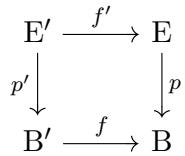
\includegraphics[keepaspectratio]{images/part003_c1a9b5e7.jpg}}

a Cartesian square. We assume that the map f is proper, separated, and surjective, and we make one of the following hypotheses:

\begin{enumerate}
\def\labelenumi{(\roman{enumi})}
\item
  The fibers of f are locally connected and the fibered square \(B^{\prime} \times_{B} B^{\prime}\) is locally connected.
\item
  The fibers of \(f\) are finite, the diagonal \(\Delta_{\mathrm{B}^{\prime}}\) of \(\mathrm{B}^{\prime}\times_{\mathrm{B}}\mathrm{B}^{\prime}\) is open in \(\mathrm{B}^{\prime}\times_{\mathrm{B}}\mathrm{B}^{\prime}\) and \(\mathrm{B}^{\prime}\times_{\mathrm{B}}\mathrm{B}^{\prime} - \Delta_{\mathrm{B}^{\prime}}\) is a locally connected space.
\end{enumerate}

Then, if \((\mathrm{E}^{\prime}, p^{\prime})\) is a covering, \((\mathrm{E}, p)\) is a covering.

Since the map \(f\) is universally strict (I, p.~20, corollary), the map \(p\) is étale (I, p.~31, prop. 8) and separated (I, p.~27, prop. 4). We shall assume, as is permissible, that \(\mathrm{E}' = \mathrm{B}' \times_{\mathrm{B}} \mathrm{E}\) .

Let \(a\) be a point of B; the aim is to show that the point \(a\) has a neighborhood W such that the W-space \((\mathrm{E_W}, p_{\mathrm{W}})\) is a trivializable covering. Set \(\mathrm{B}_a^\prime = f^{-1}(a)\) and set \(\mathrm{E}_a^\prime = (p')^{-1}(\mathrm{E}_a)\) . The map \(t_a: \mathrm{E}_a^\prime \to \mathrm{B}_a^\prime \times \mathrm{E}_a\) defined by \(t_a(y) = (p'(y), f'(y))\) is a \(\mathrm{B}_a^\prime\) -isomorphism (I, p.~9, prop. 4), hence \(\mathrm{E}_a^\prime\) is a trivializable covering of \(\mathrm{B}_a^\prime\) and \(t_a\) is a trivialization of this covering.

Let us prove that there exists a neighborhood \(V'\) of \(B'_{a}\) in \(B'\) and a continuous trivialization t of the covering ( \(E_{V'}', p_{V'}\) ) that extends \(t_{a}\) . Under hypothesis (ii), \(B'_{a}\) is finite and its points possess pairwise disjoint open neighborhoods over which the covering \(E'\) is trivializable, whence the assertion in this case. Under hypothesis (i), \(B'_{a}\) is locally connected, as is B' (IV, p.~390, lemma 1); since the map f is proper and separated, \(B'_{a}\) is compact and two distinct points have disjoint neighborhoods in B', so that the pair (B', \(B'_{a}\)) satisfies property (PCV) (I, p.~37, lemma 1). The assertion therefore follows from cor. 2 of I, p.~90.

Since \(f\) is proper, there exists a neighborhood \(V\) of \(a\) in \(B\) such that \(V'\) contains \(f^{-1}(V)\) (lemma, I, p.~75). One may thus assume that \(V' = f^{-1}(V)\) .

Equip the \(V'\)-spaces \(V' \times E_{a}\) and \(E_{V'}' = V' \times_{B} E\) with their canonical descent data relative to \(f_{V}: V' \to V\) . We shall show that, after possibly shrinking V and \(V'\), the isomorphism of \(V'\)-spaces \(t: E_{V'}' \to V' \times E_{a}\) that we have just defined is compatible with the descent data, that is, we have \(t(b_{1}', x) = t(b_{2}', x)\) if \((b_{1}', b_{2}') \in V' \times_{V} V'\) and \(x \in E_{f(b_{1}')}\) . Denote by \(\widetilde{t}\) the map \(pr_{2} \circ t: E_{V'}' \to E_{a}\) .

Let us set \(V'' = V' \times_{V} V'\) ; consider it as a \(V'\)-space by means of the first projection. The map \(((b_{1}', b_{2}'), x) \mapsto ((b_{1}', b_{2}'), (b_{1}', x))\) from \(V'' \times_{V} E\) into \(V'' \times_{V'} E'\) is an isomorphism of \(V''\)-spaces; this shows that \(V'' \times_{V} E\) is a covering of \(V''\) .

For \(i=1,2\) , we define a map \(u_{i}\colon V^{\prime\prime}\times_{V}E\to V^{\prime\prime}\times E_{a}\) by setting \(u_{i}(b_{1}^{\prime},b_{2}^{\prime},x)=(b_{1}^{\prime},b_{2}^{\prime},\widetilde{t}(b_{i}^{\prime},x))\) ; these are trivializations of the covering \(V^{\prime\prime}\times_{V}E\) . Let \(W^{\prime\prime}\) be the set of points \(w\in V^{\prime\prime}\) over which these trivializations \(u_{1}\) and \(u_{2}\) coincide; it contains \(B_{a}^{\prime}\times B_{a}^{\prime}\) , as well as the diagonal \(\Delta_{V'}\) . Let us prove that \(W^{\prime\prime}\) is a neighborhood of \(B_{a}^{\prime}\times B_{a}^{\prime}\) . Under hypothesis (i), this follows from cor. 2 of I, p.~80, since \(B^{\prime}\times B^{\prime}\) is locally connected. Under hypothesis (ii), \(W^{\prime\prime}\) contains a neighborhood of \((B_{a}^{\prime}\times B_{a}^{\prime})-\Delta_{B_{a}^{\prime}}\) in \((B^{\prime}\times_{B}B^{\prime})-\Delta_{B^{\prime}}\) , since this set is locally connected (loc. cit.). Since \(\Delta_{V'}\) is open in \(B^{\prime}\times_{B}B^{\prime}\) , \(W^{\prime\prime}\) is a neighborhood of \(B_{a}^{\prime}\times B_{a}^{\prime}\) in \(V^{\prime\prime}\) .

Since \(f\) is proper, the canonical map \(f''\) of \(\mathrm{B}' \times_{\mathrm{B}} \mathrm{B}'\) into B is proper, because it is the composite of the projection \(\mathrm{pr}_{1} \colon \mathrm{B}' \times_{\mathrm{B}} \mathrm{B}' \to \mathrm{B}'\) and of the mapping \(f\) .

By the lemma of I, p.~75, there exists a neighborhood W of a in V such that \((f'')^{-1}(\mathrm{W})\) is contained in \(W''\); set \(W'=(f')^{-1}(\mathrm{W})\), which is a subset of \(V'\) and the isomorphism of étale spaces \(t: E_{W'}' \to W' \times E_a\) is compatible with the canonical descent data relative to the map \(f_W: W' \to W\) . It follows from the corollary (IV, p.~388) that the

W-étale spaces \(E_{W}\) and \(W \times E_{a}\) are isomorphic. In particular, \(E_{W}\) is a trivializable covering, whence the proposition.

COROLLARY 1. --- Let E and B be topological spaces, \(p\colon\mathrm{E}\to\mathrm{B}\) a continuous map and \((\mathrm{A}_{i})_{i\in\mathrm{I}}\) a locally finite closed covering of B such that for every pair \((i,j)\in\mathrm{I}\times\mathrm{I}, i\neq j\) , the intersection \(\mathrm{A}_{i}\cap\mathrm{A}_{j}\) is a locally connected space. Then, for the B-space \((\mathrm{E},p)\) to be a covering, it is necessary and sufficient that, for every \(i\in\mathrm{I}\) , the \(\mathrm{A}_{i} \)-space \((p^{-1}(\mathrm{A}_{i}),p_{\mathrm{A}_{i}})\) be a covering of \(\mathrm{A}_{i}\) .

The condition is necessary (cf. I, p.~69). Conversely, let B' denote the topological sum space of the family \((\mathrm{A}_{i})_{i\in\mathrm{I}}\) and \(f\colon B'\to B\) the canonical map. The map f is closed (TG, I, p.~6, prop. 4), separated (I, p.~27, remark 5), with finite fibers, hence proper (TG, I, p.~75, th. 1); it is also surjective. The diagonal \(\Delta_{B'}\) , being equal to \(\bigcup_{i\in I}A_{i}\times_{B}A_{i}\) , is open in \(B'\times_{B}B'\) . Finally, the space \((\mathrm{B}'\times_{\mathrm{B}}\mathrm{B}')-\Delta_{\mathrm{B'}}\) is homeomorphic to the sum space of the family \((\mathrm{A}_{i}\cap\mathrm{A}_{j})\) , \((i,j)\in\mathrm{I}\times\mathrm{I}\) , \(i\neq j\) ; it is therefore locally connected. Hypothesis (ii) of proposition 6 is satisfied. If for every i, \(p^{-1}(\mathrm{A}_{i})\) is a covering of \(A_{i}\) , \(E'\) is then a covering of \(B'\) , hence E is a covering of B.

COROLLARY 2. --- Let X and Y be topological spaces and let \(f\colon X \to Y\) be a proper, separated, and surjective map. Moreover, assume one of the following hypotheses:

\begin{enumerate}
\def\labelenumi{(\roman{enumi})}
\item
  The fibers of f, as well as the space \(X\times_Y X\), are locally connected;
\item
  The fibers of \(f\) are finite, the diagonal \(\Delta_{\mathrm{X}}\) of \(\mathrm{X} \times_{\mathrm{Y}} \mathrm{X}\) is open in \(\mathrm{X} \times_{\mathrm{Y}} \mathrm{X}\) and the space \((\mathrm{X} \times_{\mathrm{Y}} \mathrm{X}) - \Delta_{\mathrm{X}}\) is locally connected. Then, every descent datum relative to \(f\) on a covering of \(\mathrm{X}\) is effective, and the quotient space is a covering of \(\mathrm{Y}\) .
\end{enumerate}

Let Z be a covering of X and let \(\tau\) be a descent datum relative to f on Z. By proposition 5 (IV, p.~389), the descent datum \(\tau\) is effective, in other words the square

\pandocbounded{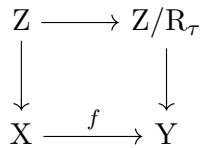
\includegraphics[keepaspectratio]{images/part003_fd3d7e4d.jpg}}

is a Cartesian square. The hypotheses of proposition 6 (IV, p.~391) are then satisfied. Consequently, \(Z/R_{\tau}\) is a covering of Y.

PROPOSITION 7. --- Let X and Y be topological spaces and let \(f: X \to Y\) be a continuous and surjective map. Suppose that Y is deloopable and that the map f is open and has the path-lifting property. Then, every descent datum relative to f on a covering of X is effective, and the quotient space is a covering of Y.

Let \((Z,p)\) be a covering of X and let \(\tau\) be a descent datum relative to f on Z. Since the map f is surjective and open, it follows from prop. 5 of IV, p.~389, that the descent datum \(\tau\) is effective. Let \(T = Y/R_{\tau}\) denote the quotient Y-space; its projection q is étale (loc. cit.), and it is also separated (I, p.~27, prop. 4).

By hypothesis, the map f has the path lifting property, as does the map p, since Z is a covering of X (III, p.~302, corollary 2 of prop. 3). Consequently, the same holds for the map \(p \circ f\) , hence for the map q. Therefore (cf.~IV, p.~341, remark 2), T is a covering of Y. The proposition is thus proved.

Remark. --- Let X and Y be topological spaces and let \(f: X \rightarrow Y\) be a map. For every descent datum relative to f on a covering of X to be effective, and for the quotient space to be a covering of Y, it is necessary that f be strict and that \(f(X)\) be an open and closed subset of X.

Indeed, identify the X-space X with \(X \times_{Y} Y\) and endow it with its canonical descent datum relative to f. The quotient space is identified with \(f(\mathrm{X})\) , equipped with the quotient topology of the topology of X for the equivalence relation defined by f. If this is a covering of Y, the space \(f(\mathrm{X})\) is then identified with an open and closed subset of Y and the map f is strict.

\subsection{Descent of groupoids}

Let X and Y be topological spaces, and let \(f\colon\mathrm{X}\to\mathrm{Y}\) be a continuous map. Let \(p_{1}\) and \(p_{2}\) be the two projections of \(\mathrm{X}\times_{\mathrm{Y}}\mathrm{X}\) into X, \(\operatorname{Coeg}(f)\) the coequalizer groupoid of the pair \((\varpi(p_{1}),\varpi(p_{2}))\) of groupoid morphisms from \(\varpi(\mathrm{X}\times_{\mathrm{Y}}\mathrm{X})\) into \(\varpi(\mathrm{X})\), and \(\gamma\colon\varpi(\mathrm{X})\to\operatorname{Coeg}(f)\) the canonical groupoid morphism (II, p.~199, def. 2). Since \(f\circ p_{1}=f\circ p_{2}\) , we have \(\varpi(f)\circ\varpi(p_{1})=\varpi(f)\circ\varpi(p_{2})\) . It then follows from the universal property of coequalizers (II, p.~199, prop. 3) that there exists a unique morphism of groupoids \(\varpi'(f)\colon\operatorname{Coeg}(f)\to\varpi(\mathrm{Y})\) such that \(\varpi(f)=\varpi'(f)\circ\gamma\) .

The set of vertices of Coeg(f) is the quotient set of the set X = Vert( \(\varpi(X)\) ) by the equivalence relation defined by f (II, p.~200, remark 1). It is identified with f(X).

PROPOSITION 8. --- Let X and Y be nonempty topological spaces and let f be a continuous map from X to Y. Suppose that X is locally path-connected, Y is connected, and f is strict and surjective. Then the groupoid Coeg(f) is transitive.

Let \(\Gamma\) be the quiver whose set of vertices is X and whose set of arrows is the disjoint union of \(\mathrm{Fl}(\varpi(\mathrm{X}))\) and \(\mathrm{X}\times_{\mathrm{Y}}\mathrm{X}\), the source and target maps being those of \(\varpi(\mathrm{X})\) on \(\mathrm{Fl}(\varpi(\mathrm{X}))\) and the maps \(p_1\) and \(p_2\) on \(\mathrm{X}\times_{\mathrm{Y}}\mathrm{X}\) . By the definition of the frame of the pair \((\varpi(\mathrm{pr}_1), \varpi(\mathrm{pr}_2))\) (II, p.~185, def. 3) and remark 2 of II, p.~200, the set of orbits of \(\operatorname{Coeg}(f)\) is identified with the set of connected components of the quiver \(\Gamma\) . Since the space X is not empty, it suffices to prove that the graph \(\Gamma\) is connected.

The connected components of \(\Gamma\) are saturated for the equivalence relation “there exists a path joining \(x\) to \(x'\) ”, hence are open in X, because X is locally path-connected. They are then also closed. They are also saturated for the equivalence relation R defined by f . By hypothesis, the map f induces a homeomorphism from X/R onto Y, so that the image under f of every connected component of \(\Gamma\) is an open and closed subset of Y, hence is equal to Y since the space Y is assumed to be connected.

Let C be a connected component of \(\Gamma\) , let \(x\) be a point of X. By the preceding, there exists a point \(x' \in \mathrm{C}\) such that \(f(x') = f(x)\) . By definition of the quiver \(\Gamma\) , we have \(x' \in \mathrm{C}\) . One thus has \(\mathrm{C} = \mathrm{X}\) and the quiver \(\Gamma\) is therefore connected.

PROPOSITION 9. --- Let X and Y be topological spaces and let f be a continuous map from X to Y. Suppose that the space X is locally path-connected, that the space Y is deloopable, and that the map f is strict and surjective. Then, the groupoid \(\varpi(\mathrm{Y})\) is generated by the image of \(\varpi(\mathrm{X})\) under \(\varpi(f)\) .

We may assume that the spaces X and Y are nonempty. Let G denote the subgroupoid of \(\varpi(\mathrm{Y})\) generated by the image of \(\varpi(\mathrm{X})\) under \(\varpi(f)\) . As the map f is surjective, the set of vertices of G is equal to Y. By prop. 8, \(\operatorname{Coeg}(f)\) is a transitive groupoid. Since \(\varpi'(f)\) induces the identity on the vertices, the image of \(\operatorname{Coeg}(f)\) under \(\varpi'(f)\) is a transitive subgroupoid of \(\varpi(\mathrm{Y})\) . The image of \(\varpi(\mathrm{X})\) under \(\gamma\) generates \(\operatorname{Coeg}(f)\) (II, p.~200, corollary); since we have \(\varpi(f) = \varpi'(f) \circ \gamma\) , the groupoid G is transitive.

Let \(y_{0}\) be a point of Y and let H denote the subgroup \(G_{y_{0}}\) of \(\pi_{1}(Y, y_{0})\) . By th. 1 of IV, p.~342, there exists a connected covering (T, p) of Y and a point \(t_{0}\) of the fiber \(T_{y_{0}}\) whose fixator is H.

If \(x\) is a point of X, the set \(\mathrm{Fl}_{y_0,f(x)}(\mathrm{G})\) is nonempty, since G is transitive. For \(u\in \mathrm{Fl}_{y_0,f(x)}(\mathrm{G})\) , the point \(t_0\cdot u\) is a point of the fiber \(\mathrm{T}_{f(x)}\) , independent of \(u\) since the group H, the isotropy group of G at \(y_0\) , fixes \(t_0\) . Denote by \(\sigma (x)\) this point; denote by \(\sigma \colon \mathrm{X}\to \mathrm{T}\) the map thus defined and \(s\colon \mathrm{X}\to \mathrm{X}\times_{\mathrm{Y}}\mathrm{T}\) the map \(x\mapsto (x,\sigma (x))\) . By construction, the map s is compatible with the canonical actions of \(\varpi (\mathrm{X})\) on X and \(\mathrm{X}\times_{\mathrm{Y}}\mathrm{T}\) . It then follows from Lemma 1 of III, p.~312, that s is continuous. The map \(\sigma\) is therefore continuous; moreover, it is compatible with the equivalence relation defined by f since \(\sigma (x)\) depends only on \(f(x)\) . Since f is strict and surjective, there exists a unique continuous map \(\overline{\sigma}\colon \mathrm{Y}\to \mathrm{T}\) such that \(\overline{\sigma}\circ f = \sigma\) , so that the covering T admits a section. Since T is connected, the map \(p\colon \mathrm{T}\to \mathrm{Y}\) is a homeomorphism (I, p.~31, cor. 4 of prop. 6) and one has \(\mathrm{H} = \pi_1(\mathrm{Y},y_0)\) , whence \(\mathrm{G}_{y_0} = \pi_1(\mathrm{Y},y_0)\) . Since G is transitive, it follows that \(\mathrm{G} = \varpi (\mathrm{Y})\) .

PROPOSITION 10. --- Let X and Y be topological spaces and let f be a continuous map from X to Y. Suppose that the space X is deloopable, that the space \(X\times_{Y}X\) is locally path-connected, and that every descent datum relative to f on a covering of X is effective and the quotient space is a covering of Y. Then, the groupoid morphism \(\varpi'(f)\) from Coeg(f) into \(\varpi(Y)\) is injective.

Under the hypotheses of the proposition, \(f\) is strict (IV, p.~394, remark); one may moreover assume that it is surjective.

Lemma 2. --- Keep the notations and hypotheses of the proposition. Let T be a set equipped with an action of the groupoid Coeg(f) relative to a map q: T → Y. Then there exists a unique topology on T for which q makes T a covering of Y such that for every path class with origin c in X and every point t in T, one has \(t \cdot \gamma(c) = t \cdot f_{*}(c)\) . In particular, the action of Coeg(f) on T factors through an action of the groupoid \(\varpi(Y)\) .

The uniqueness of such a topology on T follows from Lemma 1 (III, p.~312); let us prove its existence. Endow the set \(X\times_{Y}T\) with an action of \(\varpi(\mathrm{X})\) by setting \((x,t)\cdot u=(x\cdot u,t\cdot\gamma(u))\) for all \((x,t)\in\mathrm{X}\times_{\mathrm{Y}}\mathrm{T}\) and every arrow u with source x in \(\varpi(\mathrm{X})\). Since the space X is deloopable, this action is without local monodromy (III, p.~313, remark). There therefore exists on the set \(X\times_{Y}T\) a unique topology that makes the X-space \((\mathrm{X}\times_{\mathrm{Y}}\mathrm{T},\mathrm{pr}_{1})\) a covering of X such that the canonical action of \(\varpi(\mathrm{X})\) on this covering coincides with the given action (III, p.~313, prop. 3). Let us denote this covering by \((Z,p)\). Let us show that the map \(\tau: ((x_{1},t),x_{2})\mapsto(x_{2},t)\) from \(Z\times_{Y}X\) into Z is a descent datum on Z relative to the map f. It suffices to verify that it is continuous, the other conditions of Definition 1 of IV, p.~382, being evident.

The map \(\tau\) is a lifting of the map \(\mathrm{pr}_2\colon Z\times_Y X\to X\) to the covering \(Z\) of \(X\) . Since the space \(X\times_Y X\) is locally path-connected, the space \(Z\times_Y X\) , which is a covering of it, is also locally path-connected. By the corollary (III, p.~269), to show that the map \(\tau\) is continuous, it suffices to show that it is continuous by paths.

So let \(\widetilde{c} = ((c,g),c')\) be a path in \(Z\times_{Y}X\) and let us show that the map \(\tau \circ \widetilde{c}\colon t\mapsto (c'(t),g(t))\) from I to Z is continuous. For every \(s\in [0,1]\) , denote by \(c_s\) and \(c_s'\) the paths in X defined by \(t\mapsto c(st)\) and \(t\mapsto c'(st)\) . For all \(s\in [0,1]\) , we thus have \(c(s) = c(0)\cdot [c_s]\) , \(c'(s) = c'(0)\cdot [c_s']\) and \((c,g)(s) = (c(0),g(0))\cdot [c_s]\) , where \([u]\) denotes the strict homotopy class of a path u (III, p.~304, remark). The map \(t\mapsto (c_s(t),c_s'(t))\) is a path in \(X\times_{Y}X\) ; by definition of the coequalizer Coeg(f), we therefore have \(\gamma ([c_s]) = \gamma ([c_s'])\) and \(g(s) = g(0)\cdot \gamma ([c_s]) = g(0)\cdot \gamma ([c_s'])\) . By definition of the action of \(\varpi (X)\) on Z, we therefore have

\[
\begin{array}{r} (\tau \circ \widetilde {c}) (s) = (c ^ {\prime} (s), g (s)) = (c ^ {\prime} (0) \cdot [ c _ {s} ^ {\prime} ], g (0) \cdot \gamma ([ c _ {s} ^ {\prime} ])) \\ = (c ^ {\prime} (0), g (0)) \cdot [ c _ {s} ^ {\prime} ] = (\tau \circ \widetilde {c}) (0) \cdot [ c _ {s} ^ {\prime} ]. \end{array}
\]

This shows that \(\tau \circ \widetilde{c}\) is a continuous lift to Z of the path \(c'\) (loc. cit.). Consequently, the map \(\tau\) is continuous by paths, hence continuous; it is a descent datum relative to \(f\) on the X-space Z.

Denote by \(R_{\tau}\) the equivalence relation defined by the descent datum \(\tau\) . Since the map f is surjective, the map \(pr_{2}: Z \to T\) induces, by passing to the quotient, a bijection from \(Z/R_{\tau}\) onto T. Endow T with the topology deduced from that of \(Z/R_{\tau}\) by transport of structure, so that \((T,q)\) is a Y-space. By hypothesis, T is therefore a covering of Y and the diagram

\[
\begin{array}{c} \mathrm{Z} \xrightarrow {\mathrm{pr} _ {2}} \mathrm{T} \\ p \Big \downarrow \qquad \qquad \qquad \qquad \Big \downarrow q \\ \mathrm{X} \xrightarrow {f} \mathrm{Y} \end{array}
\]

is a Cartesian square.

Let \((x,t)\) be a point of Z, let c be a path with origin x in X, and let \(\widetilde{c}\) be the continuous lift of c to Z with origin \((x,t)\) . The path \(pr_{2} \circ \widetilde{c}\) is the lift with origin t of the path \(f \circ c\) of Y, so that \(t \cdot \gamma([c]) = t \cdot [f \circ c] = t \cdot f_{*}([c])\) . This concludes the proof of the lemma.

Let us now prove the proposition. Let \(u\) and \(v\) be two arrows of Coeg( \(f\) ) whose images in \(\varpi(Y)\) are equal. The groupoid morphism \(\varpi'(f)\) being the identity on the vertex sets, the arrows \(u\) and \(v\) have the same origin and the same target. Let us denote by \(y\) the origin of \(u\) ; let T be the set of arrows of Coeg( \(f\) ) with source y and let \(q: \mathrm{T} \to \mathrm{Y}\) the restriction to T of the target map. The groupoid Coeg( \(f\) ) acts by right composition on the set T, relative to \(q\) . By Lemma 2, the actions of \(u\) and \(v\) on T are identical. We therefore have \(u = e_y \cdot u = e_y \cdot v = v\) . This proves that the groupoid morphism \(\varpi'(f)\) is injective.

THEOREM 1. --- Let X and Y be topological spaces, let \(f: X \to Y\) be a continuous and surjective map. Suppose the spaces X and Y are deloopable. Finally, suppose that one of the following properties is satisfied:

\begin{enumerate}
\def\labelenumi{(\roman{enumi})}
\item
  The map f is proper, separated, with locally connected fibers, and the space \(X\times_{Y}X\) is locally path-connected;
\item
  The map f is proper, separated, with finite fibers, the diagonal \(\Delta_{X}\) is open in \(X \times_{Y} X\) and its complement is locally connected;
\item
  The map f is open and has the path lifting property.
\end{enumerate}

Then, the morphism of groupoids \(\varpi'(f)\) is an isomorphism from the groupoid Coeg(f) onto the Poincaré groupoid \(\varpi(Y)\) .

Let us first note that under these hypotheses, the map \(f\) is surjective and strict (I, p.~18, example 2). Moreover, every descent datum relative to \(f\) on a covering of X is effective, and the quotient space is a covering of Y; this follows from IV, p.~393, corollary 2 of prop. 4 under hypotheses (i) and (ii), and from prop. 7 of IV, p.~394 under hypothesis (iii). By prop. 10, the morphism of groupoids \(\varpi'(f)\) is therefore injective, and its image is a subgroupoid of \(\varpi(Y)\) .

By prop. 9 of IV, p.~395, this image is equal to \(\varpi(\mathrm{Y})\) under hypotheses (i) and (ii), but also under hypothesis (iii) since the groupoid morphism \(\varpi(f)\) is then surjective.

Therefore, \(\varpi'(f)\) is an isomorphism.

Examples. --- Here are two examples where the hypotheses of Theorem 1 are satisfied.

\begin{enumerate}
\def\labelenumi{\arabic{enumi})}
\item
  Let Y be a deloopable topological space. Let \((\mathrm{A}_{i})_{i\in\mathrm{I}}\) be a locally finite cover of Y by closed sets. Suppose that, for every \(i\in I\) , the space \(A_{i}\) is deloopable and that, for every pair \((i,j)\in\mathrm{I}\times\mathrm{I}\) , the space \(A_{i}\cap A_{j}\) is locally path-connected. One may take for X the sum space of the family \((\mathrm{A}_{i})_{i\in\mathrm{I}}\) and for \(f:X\to Y\) the map deduced from the family of canonical injections.
\item
  Let G be a discrete group acting properly on a deloopable topological space X; set Y = X/G and let \(f: X \to Y\) be the canonical map. It is open (TG, III, p.~10, lemma 2) and has the path-lifting property by virtue of Theorem 4 of III, p.~287. The space Y is deloopable according to IV, p.~349, prop. 8, b). By hypothesis, the map from G × X to \(X\times X\) given by \((g, x) \mapsto (g \cdot x, x)\) is proper, hence strict (I, p.~18, example 2), and its image is \(X\times_{Y}X\). It then follows from III, p.~261, prop. 8 that \(X\times_{Y}X\) is locally path-connected.
\end{enumerate}

\subsection{Descent by an étale and surjective map}

Let X and Y be topological spaces, and let f be a continuous map from X to Y. We retain the notation of the preceding section.

THEOREM 2. --- Suppose that every point of Y has a neighborhood over which there exists a continuous section of the map f. Then the groupoid morphism \(\varpi'(f)\) from \(\operatorname{Coeg}(f)\) into \(\varpi(Y)\) is an isomorphism.

By hypothesis, there exists a covering \((\mathrm{U}_{j})_{j\in\mathrm{J}}\) of Y by open sets and, for every \(j\in J\), a continuous section \(s_{j}\) of \(f_{U_{j}}\) .

If \(c\) is a path in X, we will denote by \([c]\) its strict homotopy class in \(\varpi(X)\) and by \(\{c\}\) the image of \([c]\) in \(\operatorname{Coeg}(f)\) under the groupoid morphism \(\gamma\) . If \(c\) and \(c'\) are two paths in X, \(\{c\}\) and \(\{c'\}\) are composable in \(\operatorname{Coeg}(f)\) if and only if the paths \(f \circ c\) and \(f \circ c'\) in Y are juxtaposable.

Let \(c'\) be a path in Y. By Lemma 4 of III, p.~272, applied to the compact space I and the covering \(((c')^{-1}(\mathrm{U}_j))_{j\in \mathrm{J}}\) of I, there exists an integer \(n\) such that, for every integer \(k\) satisfying \(1\leqslant k\leqslant n\), the image of the interval \([\frac{k - 1}{n},\frac{k}{n}]\) under \(c'\) is contained in an open set \(\mathrm{U}_{j(k)}\) . For every integer \(k\) , \(1\leqslant k\leqslant n\) , let \(c_k'\) be the path in Y defined by \(s\mapsto c'(\frac{k + s - 1}{n})\) ; we have \([c'] = [c_1'][c_2']\ldots [c_n']\) (cf. III, p.~291, Remark 1), and \(c'\) is the path denoted \(c_1' * c_2' * \dots * c_n'\) . For all \(k\in \{1,\ldots ,n\}\) , denote by \(c_k\) the path \(s_{j(k)}\circ c_k'\) in X and set \(\{c_k\} = \gamma ([c_k])\) . Since for every \(k\) the paths \(c_{k - 1}' = f\circ c_{k - 1}\) and \(c_k' = f\circ c_k\) are juxtaposable, the sequence \((\{c_1\} ,\ldots ,\{c_n\})\) is composable in \(\operatorname{Coeg}(f)\). By construction,

\[
\begin{array}{r l} & {\varpi^ {\prime} (f) (\{c _ {1} \} \ldots \{c _ {n} \}) = \varpi^ {\prime} (f) (\{c _ {1} \}) \ldots \varpi^ {\prime} (f) (\{c _ {n} \})} \\ & {\qquad = \varpi (f) ([ c _ {1} ]) \ldots \varpi (f) ([ c _ {n} ])} \\ & {\qquad = [ f \circ c _ {1} ] \ldots [ f \circ c _ {n} ]} \\ & {\qquad = [ c _ {1} ^ {\prime} ] * \dots * [ c _ {n} ^ {\prime} ] = [ c ^ {\prime} ],} \end{array}
\]

which proves that the groupoid morphism \(\varpi'(f)\) is surjective.

Let \(u\) and \(v\) be arrows of \(\operatorname{Coeg}(f)\) . Since the groupoid \(\operatorname{Coeg}(f)\) is generated by the image of \(\varpi(\mathrm{X})\) (II, p.~200, corollary), there exist finite sequences \((c_1, \ldots, c_n)\) and \((d_1, \ldots, d_n)\) of paths in X such that one has \(u = \{c_1\} \ldots \{c_n\}\) and \(v = \{d_1\} \ldots \{d_n\}\) . The paths \((f \circ c_1, \ldots, f \circ c_n)\) in Y are then juxtaposable and one has \(\varpi'(f)(u) = [(f \circ c_1)] \ldots [(f \circ c_n)]\) ; likewise, \(\varpi'(f)(v) = [(f \circ d_1)] \ldots [(f \circ d_n)]\) .

Suppose that we have \(\varpi'(f)(u) = \varpi'(f)(v)\) . There then exists a strict homotopy \(\sigma\) connecting \((f \circ c_1) * \cdots * (f \circ c_n)\) to \((f \circ d_1) * \cdots * (f \circ d_n)\) . By Lemma 4 of III, p.~272, applied to the compact space \(\mathbf{I} \times \mathbf{I}\) and the covering \((\bar{\sigma}^{-1}(\mathrm{U}_i))_{i \in \mathrm{I}}\) of \(\mathbf{I} \times \mathbf{I}\) , there exists an integer \(m \geqslant 1\) such that, for every pair of integers \((j,k)\) satisfying \(1 \leqslant j \leqslant m\) and \(1 \leqslant k \leqslant m\), the image of \([\frac{j-1}{m}, \frac{j}{m}] \times [\frac{k-1}{m}, \frac{k}{m}]\) under \(\sigma\) is contained in an open set \(U_{i(j,k)}\) of the covering \((\mathrm{U}_{i})_{i \in \mathrm{I}}\) .

Every path c in X is of the form \(c_{1}*\cdots*c_{m}\) , where \(c_{k}\) is the path \(t\mapsto c(\frac{k-1+t}{m})\) . If necessary, replacing the integers m and n by their product mn, one may therefore suppose that m=n.

For every pair \((j,k)\) of integers of \(\{1,\ldots ,n\}\) and every pair \((s,t)\in\) \(\mathbf{I}\times \mathbf{I}\) , set

\[
\sigma_ {j, k} (s, t) = s _ {i (j, k)} \circ \sigma \left(\frac {s + j - 1}{n}, \frac {t + k - 1}{n}\right).
\]

For \(t \in \mathbf{I}\) , also set \(h_{j,k}^{0}(t) = \sigma_{j,k}(t,0)\) , \(h_{j,k}^{1}(t) = \sigma_{j,k}(t,1)\) , \(v_{j,k}^{0}(t) = \sigma_{j,k}(0,t)\) and \(v_{j,k}^{1}(t) = \sigma_{j,k}(1,t)\) . By Lemma 1 of III, p.~295, the paths \(h_{j,k}^{0} * v_{j,k}^{1}\) and \(v_{j,k}^{0} * h_{j,k}^{1}\) are strictly homotopic, whence the relation

\[
[ h _ {j, k} ^ {0} ] [ v _ {j, k} ^ {1} ] = [ v _ {j, k} ^ {0} ] [ h _ {j, k} ^ {1} ]\tag{2}
\]

on \(\varpi(\mathrm{X})\) , for every pair \((j,k) \in \{1, \ldots, n\}^2\) . On the other hand, for every pair of integers \((j,k)\) , with \(2 \leqslant j \leqslant n\) and \(1 \leqslant k \leqslant n\) , we have \(f \circ v_{j,k}^0 = f \circ v_{j-1,k}^1\) , whence the relation

\[
\{v _ {j, k} ^ {0} \} = \{v _ {j - 1, k} ^ {1} \}\tag{3}
\]

in Coeg(f). Likewise, for every pair of integers \((j,k)\) such that \(1 \leqslant j \leqslant n\) and \(2 \leqslant k \leqslant n\) , we have

\[
\{h _ {j, k} ^ {0} \} = \{h _ {j, k - 1} ^ {1} \}.\tag{4}
\]

For \(j \in \{1, \ldots, n\}\) the paths \(f \circ c_j\) and \(f \circ h_{j,1}^0\) coincide. By definition of the coequalizer Coeg(f), one therefore has \(\{c_j\} = \{h_{j,1}^0\}\) . Likewise, for every \(j \in \{1, \ldots, n\}\) , \(\{d_j\} = \{h_{j,n}^1\}\) . Consequently, one has the relations

\[
u = \{h _ {1, 1} ^ {0} \} \dots \{h _ {n, 1} ^ {0} \}, \quad v = \{h _ {1, n} ^ {1} \} \dots \{h _ {n, n} ^ {1} \}.
\]

By Lemma 3 below, one has

\[
\{h _ {1, 1} ^ {0} \} \dots \{h _ {1, n} ^ {0} \} \{v _ {1, n} ^ {1} \} \dots \{v _ {n, n} ^ {1} \} = \{v _ {1, 1} ^ {0} \} \dots \{v _ {n, 1} ^ {0} \} \{h _ {n, 1} ^ {1} \} \dots \{h _ {n, n} ^ {1} \}.
\]

Since the paths \(t \mapsto \sigma(0,t)\) and \(t \mapsto \sigma(1,t)\) are constant, one has, for \(1 \leqslant k \leqslant n\) , \(\{v_{1,k}^{0}\} = e_{a}\) and \(\{v_{n,k}^{1}\} = e_{b}\) where \(a,b \in Y\) are the source and the target of the arrows \(u\) and \(v\) of Coeg( \(f\) ). It follows that one has the equality

\[
\{h _ {1, 1} ^ {0} \} \dots \{h _ {1, n} ^ {0} \} = \{h _ {n, 1} ^ {0} \} \dots \{h _ {n, n} ^ {1} \},
\]

that is, u = v.

Lemma 3. --- Let G be a groupoid and let p, q be integers \(\geqslant 1\) . For every pair \((j, k)\) of integers such that \(0 \leqslant j \leqslant p\) and \(0 \leqslant k \leqslant q\) , let \(x_{j,k}\) be a vertex of G; for every pair \((j, k)\) such that \(1 \leqslant j \leqslant p\) and \(0 \leqslant k \leqslant q\) , let \(h_{j,k}\) be an arrow of G connecting \(x_{j-1,k}\) to \(x_{j,k}\) ; for every pair \((j, k)\) such that \(0 \leqslant j \leqslant p\) and \(1 \leqslant k \leqslant q\) , let \(v_{j,k}\) be an arrow of G connecting \(x_{j,k-1}\) to \(x_{j,k}\) .

Suppose that, for every pair \((j,k)\) of integers such that \(1 \leqslant j \leqslant p\) and \(1 \leqslant k \leqslant q\) , the arrows \(v_{j-1,k}\) and \(h_{j,k}\) are composable, as are the arrows \(h_{j,k-1}\) and \(v_{j,k}\) , and that one has \(v_{j-1,k}h_{j,k} = h_{j,k-1}v_{j,k}\) . Then,

\[
h _ {1, 0} h _ {2, 0} \dots h _ {p, 0} v _ {p, 1} v _ {p, 2} \dots v _ {p, q} = v _ {0, 1} v _ {0, 2} \dots v _ {0, q} h _ {1, q} h _ {2, q} \dots h _ {p, q}.
\]

First treat the particular case where q = 1 and prove the result by induction on p. If p = 1, the assertion to be proved is verified by hypothesis; suppose it is verified for p - 1; one then has

\[
h _ {1, 0} h _ {2, 0} \dots h _ {p, 0} v _ {p, 1} = h _ {1, 0} h _ {2, 0} \dots h _ {p - 1, 0} v _ {p - 1, 1} h _ {p, 1} = v _ {0, 1} h _ {1, 1} \dots h _ {p, 1}
\]

by the induction hypothesis, whence the relation for p.

Now prove the result by induction on q. It is true for q = 1 by what precedes; if it is true for q - 1, one then has

\[
h _ {1, 0} h _ {2, 0} \dots h _ {p, 0} v _ {p, 1} v _ {p, 2} \dots v _ {p, q} = v _ {0, 1} v _ {0, 2} \dots v _ {0, q - 1} h _ {1, q - 1} \dots h _ {p, q - 1} v _ {p, q}.
\]

By the case \(q = 1\) , we have

\[
h _ {1, q - 1} \dots h _ {p, q - 1} v _ {p, q} = v _ {0, q} h _ {1, q} \dots h _ {p, q},
\]

whence the desired relation.

Examples. --- 1) The theorem applies when the map f is étale and surjective.

\begin{enumerate}
\def\labelenumi{\arabic{enumi})}
\setcounter{enumi}{1}
\tightlist
\item
  It also applies when the space X is the sum space of a family \((V_{i})_{i\in\mathrm{I}}\) of subsets of Y whose interiors cover Y, and f is the map deduced from the canonical injections of each of the \(V_{i}\) in Y.
\end{enumerate}

\subsection{Poincaré groupoid of a quotient space}

Let X be a topological space equipped with a continuous action of a discrete group G; set Y = X/G and denote by \(f: X \to Y\) the canonical map. Denote by \(\lvert G\rvert\) the groupoid \(\varpi(G)\); its set of vertices is G; for \(g, g' \in G\) , there exists a unique arrow from g to \(g'\) if \(g' = g\) and none otherwise. By passing to fundamental groupoids, the operation \(m: G \times X \to X\) induces a morphism of groupoids \(\varpi(m): \lvert G\rvert \times \varpi(X) \to \varpi(X)\) . Let \(\varpi(X)/G\) be the coequalizer of the two morphisms of groupoids \(\varpi(m)\) and \(\varpi(\mathrm{pr}_{2})\) of \(\lvert G\rvert \times \varpi(X)\) into \(\varpi(X)\) ; let us denote by \(\beta: \varpi(X) \to \varpi(X)/G\) the canonical morphism of groupoids. We have \(f \circ m = f \circ pr_{2}\) , therefore \(\varpi(f) \circ \varpi(m) = \varpi(f) \circ \varpi(\mathrm{pr}_{2})\) . By the universal property of coequalizers, there therefore exists a unique morphism of groupoids \(\varpi''(f): \varpi(X)/G \to \varpi(Y)\) such that one has \(\varpi(f) = \varpi''(f) \circ \beta\) .

THEOREM 3. --- Let X be a deloopable topological space and let G be a discrete group acting properly on X; let \(f\colon X \to X/G\) be the canonical surjection. The canonical groupoid morphism \(\varpi''(f)\colon \varpi(X)/G \to \varpi(X/G)\) introduced above is an isomorphism.

Denote by \(\operatorname{Coeg}(f)\) the coequalizer of the two groupoid morphisms from \(\varpi(\mathrm{X} \times_{\mathrm{Y}} \mathrm{X})\) into \(\varpi(\mathrm{X})\) induced by the projections \(pr_{1}\) and \(pr_{2}\) ; let \(\gamma: \varpi(\mathrm{X}) \to \operatorname{Coeg}(f)\) be the canonical groupoid morphism. The image of the map \((m, pr_{2})\) : \(G \times X \to X \times X\) being the subspace \(X \times_{Y} X\) of \(X \times X\) , the two groupoid morphisms \(\gamma \circ \varpi(m)\) and \(\gamma \circ \varpi(pr_{2})\) of \(\lvert G\rvert \times \varpi(X)\) into \(\operatorname{Coeg}(f)\) are equal. By the universal property of \(\varpi(\mathrm{X})/\mathrm{G}\) , there exists a unique morphism of groupoids \(\alpha: \varpi(\mathrm{X})/\mathrm{G} \to \operatorname{Coeg}(f)\) such that \(\gamma = \alpha \circ \beta\) .

We also denote by \(\varpi'(f)\) the unique groupoid morphism from \(\operatorname{Coeg}(f)\) into \(\varpi(Y)\) such that \(\varpi(f) = \varpi'(f) \circ \gamma\) . By IV, p.~399, example 2, the hypotheses of th. 1 of IV, p.~398 are satisfied and the morphism \(\varpi'(f)\) is an isomorphism. Since

\[
\varpi (f) = \varpi^ {\prime} (f) \circ \gamma = \varpi^ {\prime} (f) \circ \alpha \circ \beta = \varpi^ {\prime \prime} (f) \circ \beta ,
\]

we have \(\varpi''(f) = \varpi'(f) \circ \alpha\) . Thus, to prove Theorem 3, it suffices to show that the morphism \(\alpha\) is an isomorphism.

Lemma 4. --- For every path \(c = (c_1, c_2)\) in \(X \times_Y X\) , we have \(\beta([c_1]) = \beta([c_2])\) .

Let c be such a path.

Let \(x \in X\) , let \(K_x\) be its stabilizer in G. By TG, III, p.~32, prop. 8, there exists an open neighborhood \(U_x\) of \(x\) in X such that \(K_x \cdot U_x = U_x\),

\(g \cdot U_x \cap U_x = \varnothing\) for all \(g \in G - K_x\) and such that the map f induces a homeomorphism from \(U_x/K_x\) onto an open neighborhood \(V_x\) of \(f(x)\) in Y. Since X is deloopable and the restriction to \(U_x\) of the map f is open and closed, one may moreover assume that \(U_x\) is connected and that the image of the canonical homomorphism \(\pi_1(U_x, x) \to \pi_1(X, x)\) is reduced to the identity element. The open sets \((V_x)_{x \in X}\) thus constructed form an open covering of Y. By Lemma 4 of III, p.~272, applied to the compact space I and the open sets \((f \circ c_1)^{-1}(V_x)\) for \(x \in X\) , there exists an integer \(n \geqslant 1\) such that for every \(i \in \{1, \ldots, n\}\) , there exists a point \(x_i\) in X such that \(c_1([i-1/n, i/n])\) is contained in \(f(V_{x_i})\) . Since \(f \circ c_1 = f \circ c_2\) , \(c_2([i-1/n, i/n])\) is also contained in \(f(V_{x_i})\) .

For \(j = 1\) or 2 and for \(i \in \{1, \ldots, n\}\) , denote by \(c_{j,i}\) the path in X defined by \(t \mapsto c_j(\frac{i+t-1}{n})\) ; we have \(c_j = c_{j,1} * \cdots * c_{j,n}\) (III, p.~291, remark 1). Consequently, to show that \(\beta([c_1]) = \beta([c_2])\) , it suffices to show that \(\beta([c_{1,i}]) = \beta([c_{2,i}])\) for every integer \(i \in \{1, \ldots, n\}\) . Replacing the path \((c_1, c_2)\) by the path \((c_{1,i}, c_{2,i})\) , we may thus assume that there exists \(x \in X\) such that \((f \circ c_1)([0,1]) \subset V_x\) .

The inverse image of \(V_{x}\) under f is the disjoint union of the connected components \(g \cdot U_{x}\) where g runs over a system of representatives in G of \(G/K_{x}\) . For i = 1 or 2, let \(g_{i}\) be an element of G such that the point \(x_{i} = g_{i} \cdot c_{i}(0)\) belongs to \(U_{x}\) . The image of the path \(g_{i} \cdot c_{i}\) is then contained in \(U_{x}\) . By definition of the groupoid \(\varpi(\mathrm{X})/\mathrm{G}\) , we have \(\beta([g_{i} \cdot c_{i}]) = \beta([c_{i}])\) which allows us to assume that the images of the paths \(c_{1}\) and \(c_{2}\) are contained in \(U_{x}\) and that \(g_{1} = g_{2} = e\) .

For \(s=0\) or 1, let \(d_{s}\) be a path in \(\mathrm{U}_{x}\) connecting \(x\) to \(c_{1}(s)\) and let \(g_{s}\) be an element of \(\mathrm{K}_{x}\) such that \(g_{s}\cdot c_{2}(s)=c_{1}(s)\) . The paths \(d_{0}*c_{1}*\overline{d_{1}}\) and \(d_{0}*(g_{0}\cdot c_{2})*(g_{0}g_{1}^{-1}\cdot\overline{d_{1}})\) are loops at \(x\) on \(\mathrm{U}_{x}\) . They are therefore strictly homotopic in X to the constant loop at \(x\) , because the image of the canonical homomorphism \(\pi_{1}(\mathrm{U}_{x},x)\to\pi_{1}(\mathrm{X},x)\) is reduced to the identity element. Their classes in particular have the same image under the groupoid morphism \(\beta\) , whence

\[
\beta ([ d _ {0} ]) \beta ([ c _ {1} ]) \beta ([ d _ {1} ]) ^ {- 1} = \beta ([ d _ {0} ]) \beta ([ g _ {0} \cdot c _ {2} ]) \beta ([ g _ {0} g _ {1} ^ {- 1} \cdot d _ {1} ]) ^ {- 1}.
\]

Since \(\beta([g \cdot c]) = \beta([c])\) for every element \(g \in G\) and for every path \(c\) in \(X\) , the equality \(\beta([c_1]) = \beta([c_2])\) follows, as was to be proved.

By the lemma, the two groupoid morphisms \(\beta \circ \varpi(\mathrm{pr}_{1})\) and \(\beta \circ \varpi(\mathrm{pr}_{2})\) from \(\varpi(\mathrm{X} \times_{\mathrm{Y}} \mathrm{X})\) into \(\operatorname{Coeg}(f)\) are equal. By the universal property of the coequalizer, there therefore exists a unique groupoid morphism \(\alpha'\) : \(\operatorname{Coeg}(f) \to \varpi(\mathrm{X})/\mathrm{G}\) such that \(\beta = \alpha' \circ \gamma\) . The morphism \(\alpha' \circ \alpha\) is the unique groupoid morphism \(\varphi\) of \(\varpi(\mathrm{X})/\mathrm{G}\) into itself such that \(\varphi \circ \beta = \beta\) ; one therefore has \(\alpha' \circ \alpha = \operatorname{Id}_{\varpi(\mathrm{X})/\mathrm{G}}\) . Likewise, \(\alpha \circ \alpha' = \operatorname{Id}_{\operatorname{Coeg}(f)}\) . Consequently, \(\alpha\) is an isomorphism.

\section{VAN KAMPEN'S THEOREM}
% semantic-fragments: legacy-input-seam
\relax{}
\subsection{Coequalizer of the projections of a fibered square}

Let X and Y be topological spaces, and let f be a continuous map from X to Y. Denote by Z the fibered square \(X \times_{Y} X\) and by \(p_{1}\) , \(p_{2}\) the two projections from Z to X. We denote by W the fibered product \(X \times_{Y} X \times_{Y} X\) ; for every pair \((s, t)\) of elements of \(\{1,2,3\}\) , we denote by \(q_{st}: W \to Z\) the map defined by \(q_{st}(x_{1}, x_{2}, x_{3}) = (x_{s}, x_{t})\) .

Denote by \(\operatorname{Coeg}(f)\) the groupoid \(\operatorname{Coeg}(\varpi(p_{1}),\varpi(p_{2}))\) , the coequalizer of the two morphisms \(\varpi(p_{1})\) , \(\varpi(p_{2})\) from the Poincaré groupoid \(\varpi(Z)\) into the Poincaré groupoid \(\varpi(X)\) . Denote by \(\gamma\colon\varpi(X)\to\operatorname{Coeg}(f)\) the canonical groupoid morphism. Since \(f\circ p_{1}=f\circ p_{2}\) , the groupoid morphisms \(\varpi(f)\circ\varpi(p_{1})\) and \(\varpi(f)\circ\varpi(p_{2})\) from \(\varpi(Z)\) into \(\varpi(Y)\) are equal; there therefore exists a unique groupoid morphism \(\varpi'(f)\colon\operatorname{Coeg}(f)\to\varpi(Y)\) such that \(\varpi'(f)\circ\gamma=\varpi(f)\) .

DEFINITION 1. --- We say that the map f satisfies property (VK) if it is strict, surjective, and if the morphism \(\varpi'(f)\) is an isomorphism.

Example 1. --- This property holds under one of the following hypotheses:

\begin{enumerate}
\def\labelenumi{(\roman{enumi})}
\item
  The spaces X and Y are delaceable, the space \(X \times_{Y} X\) is locally path-connected, the map f is surjective, proper, separated, with locally connected fibers;
\item
  The spaces X and Y are delaceable, the map f is surjective, proper, separated, with finite fibers, the diagonal \(\Delta_{X}\) of \(X \times_{Y} X\) is open and its complement is locally connected;
\item
  The spaces X and Y are delaceable, the map f is surjective, open, and has the path-lifting property;
\item
  Every point of Y has a neighborhood above which there exists a continuous section of the map f.
\end{enumerate}

Indeed, under each of these hypotheses, the map \(f\) is surjective; it is also strict by virtue of I, p. 18, example 2. Finally, the morphism \(\varpi'(f)\) is an isomorphism, whether under hypotheses (i), (ii), or (iii) according to IV, p. 398, th. 1, or under hypothesis (iv) (IV, p. 400, th. 2).

Proposition 5 of II, p. 208 describes the isotropy groups of the groupoid Coeg(f). The aim of this section is to make explicit, when f satisfies property (VK), the description of the Poincaré groups of Y that follows from it by composition with the groupoid isomorphism \(\varpi'(f)\). The following numbers will be devoted to important special cases.

Suppose that the map f satisfies property (VK).

Let us set \(\mathsf{I} = \pi_0(\mathrm{X})\) , \(\mathsf{J} = \pi_0(\mathrm{Z})\) , \(\mathsf{K} = \pi_0(\mathrm{W})\) ; for \(j \in \mathsf{J}\) and \(s \in \{1,2\}\) we set \(i_s(j) = \pi_0(p_s)(j)\) ; for \(k \in \mathsf{K}\) and \(s\) , \(t \in \{1,2,3\}\) we set \(j_{st}(k) = \pi_0(q_{st})(k)\) . Denote by \(\Gamma\) the frame of the pair \((\varpi(p_1), \varpi(p_2))\) of groupoid morphisms from \(\varpi(\mathrm{Z})\) into \(\varpi(\mathrm{X})\) (II, p. 185, def. 3). This is the quiver \((\mathsf{I}, \mathsf{J}, \pi_0(p_1), \pi_0(p_2))\) , for the orbits of the Poincaré groupoid of a topological space are the path-connected components of that space.

Suppose moreover that Y is path-connected and nonempty. By II, p. 200, remark 2, \(\pi_0(\Gamma)\) is then in bijection with the set of orbits of the groupoid Coeg(f); since the map \(f\) satisfies property (VK), the groupoid Coeg(f) is isomorphic to the groupoid \(\varpi(Y)\) . The graph \(\Gamma\) is thus connected and nonempty.

Let us call the van Kampen data of f the data consisting of the following elements:

\begin{enumerate}
\def\labelenumi{(\roman{enumi})}
\item
  for all \(i \in \mathsf{I}\) a point \(\mathsf{a}(i)\) of the path-connected component \(i\) of \(\mathbf{X}\) ;
\item
  for all \(j \in J\) a point \(\mathsf{b}(j) = (\mathsf{b}_{1}(j), \mathsf{b}_{2}(j))\) of the path-connected component j of Z;
\item
  for all \(k \in \mathsf{K}\) a point \(\mathsf{c}(k) = (\mathsf{c}_1(k), \mathsf{c}_2(k), \mathsf{c}_3(k))\) of the path-connected component \(k\) of \(\mathbf{W}\) ;
\item
  for all \(j \in J\) the class \(\beta_{1}(j)\) of a path in X connecting \(\mathsf{b}_{1}(j)\) to \(\mathsf{a}(i_{1}(j))\) and the class \(\beta_{2}(j)\) of a path in X connecting \(\mathsf{b}_{2}(j)\) to \(\mathsf{a}(i_{2}(j))\) ;
\item
  for all \(k \in K\) and for every pair \((s, t)\) equal to \((1, 2)\) , \((2, 3)\) or \((1, 3)\) the class \(\gamma_{st}(k)\) of a path in Z connecting \((\mathsf{c}_{s}(k), \mathsf{c}_{t}(k))\) to \(\mathsf{b}(j_{st}(k))\) ;
\item
  a subquiver \(\mathsf{T}\) of \(\Gamma\) whose associated graph is a maximal tree of the graph \(\widetilde{\Gamma}\) ;
\item
  an element \(i_{0}\) of \(\mathsf{I}\) .
\end{enumerate}

Let us choose a van Kampen datum of \(f\) . Then, \((\mathsf{a},\mathsf{b},\beta_{1},\beta_{2},\mathsf{T},i_{0})\) is a basic datum of the pair \((\varpi(p_{1}),\varpi(p_{2}))\) of groupoid morphisms from \(\varpi(\mathrm{Z})\) on \(\varpi(\mathrm{X})\) (II, p. 192, def. 4). Moreover, the triples

\[
\mathsf {z} = \left(\left(q _ {1 2} (\mathsf {c} (k)), 1\right), \left(q _ {2 3} (\mathsf {c} (k)), 1\right), \left(q _ {1 3} (\mathsf {c} (k)), - 1\right)\right)
\]

and the path classes \((\gamma_{1,2}(k), \gamma_{2,3}(k), \gamma_{1,3}(k))\) , where k ranges over K, define a complementary equipment of the pair \((\varpi(p_{1}), \varpi(p_{2}))\) (II, p. 208, def. 3; II, p. 205, example; II, p. 205, remark). We shall say that the complete equipment of the coequalizer Coeg(f) thus defined is deduced from the van Kampen datum of f that we have chosen.

For every \(j \in J\) , denote by \(\varphi_{j} \colon \pi_{1}(Z, \mathsf{b}(j)) \to \pi_{1}(X, \mathsf{a}(i_{1}(j)))\) and \(\psi_{j} \colon \pi_{1}(Z, \mathsf{b}(j)) \to \pi_{1}(X, \mathsf{a}(i_{2}(j)))\) the group homomorphisms defined by

\[
\varphi_ {j} = \operatorname{Int} (\beta_ {1} (j)) ^ {- 1} \circ (p _ {1}) _ {*}, \quad v \mapsto \beta_ {1} (j) ^ {- 1} ((p _ {1}) _ {*} (v)) \beta_ {1} (j)\tag{1}
\]

\[
\psi_ {j} = \mathrm{Int} (\beta_ {2} (j)) ^ {- 1} \circ (p _ {2}) _ {*}, \quad v \mapsto \beta_ {2} (j) ^ {- 1} ((p _ {2}) _ {*} (v)) \beta_ {2} (j),
\]

for \(v \in \pi_1(\mathbf{Z}, \mathfrak{b}(j))\) . For all \(k \in \mathsf{K}\) and every \(s \in \{1,2,3\}\) , denote by \(\lambda_s(k)\) the loop class at the point \(\mathfrak{a}(i_s(k))\) in X defined by

\[
\lambda_ {1} (k) = \beta_ {1} (j _ {1 3} (k)) ^ {- 1} \cdot ((p _ {1}) _ {*} (\gamma_ {1 3} (k))) ^ {- 1} \cdot ((p _ {1}) _ {*} (\gamma_ {1 2} (k))) \cdot \beta_ {1} (j _ {1 2} (k)),\tag{2}
\]

\[
\lambda_ {2} (k) = \beta_ {2} (j _ {1 2} (k)) ^ {- 1} \cdot ((p _ {2}) _ {*} (\gamma_ {1 2} (k))) ^ {- 1} \cdot ((p _ {1}) _ {*} (\gamma_ {2 3} (k))) \cdot \beta_ {1} (j _ {2 3} (k)),
\]

\[
\lambda_ {3} (k) = \beta_ {2} (j _ {2 3} (k)) ^ {- 1} \cdot ((p _ {2}) _ {*} (\gamma_ {2 3} (k))) ^ {- 1} \cdot ((p _ {2}) _ {*} (\gamma_ {1 3} (k))) \cdot \beta_ {2} (j _ {1 3} (k)).
\]

Denote by \(\tau\) the unique morphism of groupoids from Grp \((\Gamma)\) into \(\varpi(\mathrm{Y})\) such that the map Som \((\tau)\) maps \(i \in \mathsf{I}\) to \(f(\mathsf{a}(i))\) and Fl \((\tau)\) maps \(j \in \mathsf{J}\) to the class of paths \(f_{*}(\beta_{1}(j))^{-1}f_{*}(\beta_{2}(j))\) connecting \(f(\mathsf{a}(i_{1}(j)))\)

\pandocbounded{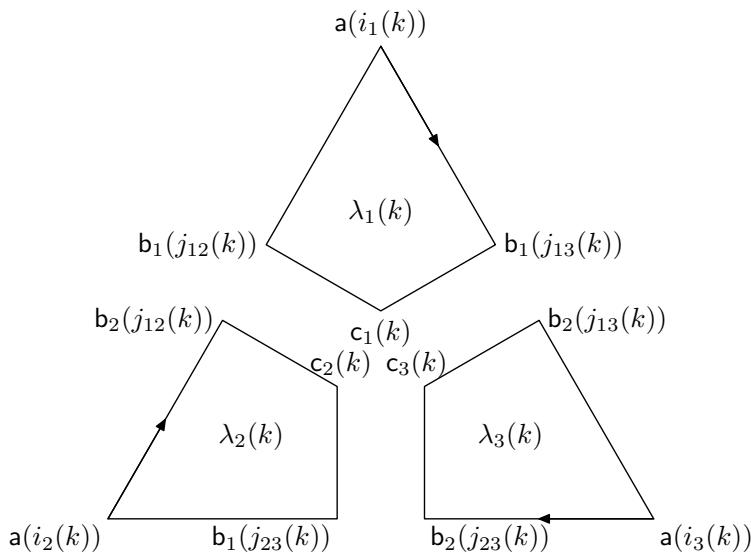
\includegraphics[keepaspectratio]{images/part003_b82e0de6.jpg}}

to \(f(\mathsf{a}(i_2(j)))\) in Y. For \(i \in \mathsf{I}\) , let \(d_i \in \mathrm{Grp}(\Gamma)\) be the class of the unique path without backtracking joining \(i_0\) to \(i\) in the tree \(\widetilde{\mathsf{T}}\) and let us set \(\delta_i = \tau(d_i)\) .

If S is a set, recall that F(S) denotes the free group on S; the image in F(S) of an element \(s \in S\) under the canonical map is denoted {[}s{]}, or even s if there is no possible confusion.

THEOREM 1. --- Suppose that Y is path-connected and that f satisfies property (VK). With the previous notation, there exists a unique group homomorphism

\[
\mathsf {L} \colon \big (\underset {i \in \mathsf {I}} {\ast} \pi_ {1} (\mathrm{X}, \mathsf {a} (i)) \big) \ast \mathrm{F} (\mathrm{J}) \to \pi_ {1} (\mathrm{Y}, f (\mathsf {a} (i _ {0})))
\]

such that

\[
\begin{array}{l l} \mathsf {L} (v) = \delta_ {i} f _ {*} (v) \delta_ {i} ^ {- 1} & \text {for } i\in I \text { and } v\in\pi_{1} (X,a(i)), \\ \mathsf {L} (j) = \delta_ {i _ {1} (j)} \tau (j) \delta_ {i _ {2} (j)} ^ {- 1} & \text {for } j\in J. \end{array}
\]

Moreover, the homomorphism L is surjective and its kernel is the smallest normal subgroup containing the following elements:

\[
\left(\mathrm{R} _ {1}\right) \quad \mathrm{r} _ {1} (j) = j \quad \text {for } j \text { in } \operatorname{Fl} (\mathsf {T});
\]

\[
\left(\mathrm{R} _ {2}\right) \quad \mathfrak {r} _ {2} (j, v) = \varphi_ {j} (v) j \psi_ {j} (v) ^ {- 1} j ^ {- 1} \quad \text {for } j \in \mathsf {J} \text { and } v \in \pi_ {1} (\mathrm{Z}, \mathfrak {b} (j));
\]

\[
\left(\mathrm{R} _ {3}\right) \quad \mathrm{r} _ {3} (k) = \lambda_ {1} (k) j _ {1 2} (k) \lambda_ {2} (k) j _ {2 3} (k) \lambda_ {3} (k) j _ {1 3} (k) ^ {- 1}, \quad \text {for } k \in \mathsf {K}.
\]

The existence and uniqueness of the homomorphism L follow from the universal property of free products and free groups. Moreover, this homomorphism is the composite of the homomorphism \(\varpi'(f)_{\gamma(\mathsf{a}(i_0))}\) deduced from \(\varpi'(f)\) by passing to isotropy groups and to the group homomorphism \(\lambda\) defined by prop. 5 of II, p. 208, taking into account that the chosen van Kampen datum determines a complete equipment of the pair \((\varpi(p_1), \varpi(p_2))\) of groupoid morphisms from \(\varpi(\mathrm{Z})\) into \(\varpi(\mathrm{X})\) . By this proposition, the homomorphism \(\lambda\) has as image the group \(\operatorname{Coeg}(f)_{\gamma(\mathsf{a}(i_0))}\) and its kernel is the smallest normal subgroup containing the elements defined by the relations \((\mathrm{R}_1)\) , \((\mathrm{R}_2)\) and \((\mathrm{R}_3)\) . On the other hand, the groupoid morphism \(\varpi'(f)\) : \(\operatorname{Coeg}(f) \to \varpi(\mathrm{Y})\) is an isomorphism, by definition of property (VK). The theorem is therefore proved.

\subsection{Coverings}

Let Y be a path-connected, nonempty topological space, and let \((\mathrm{A}_{i})_{i\in\mathrm{I}}\) be a covering of Y by nonempty path-connected subsets, indexed by a totally ordered set I. Let \(X=\bigsqcup_{i\in I}A_{i}\) be the sum space of the family \((\mathrm{A}_{i})\) and let \(f:X\to Y\) be the map induced by the family of canonical injections of each \(A_{i}\) in Y. Suppose that the map f satisfies property (VK). This holds in particular in the following two cases:

\begin{enumerate}
\def\labelenumi{(\roman{enumi})}
\item
  the interiors of the sets \(A_{i}\) , for \(i \in I\) cover Y (cf. IV, p. 402, example 2);
\item
  the space Y is delaceable, as are the spaces \(A_{i}\) , for \(i \in I\) , the family \((\mathrm{A}_{i})_{i \in \mathrm{I}}\) is locally finite, the \(A_{i}\) are closed in Y and their pairwise intersections are locally arcwise connected (cf. IV, p. 399, example 1).
\end{enumerate}

Let J' be the set of triples \((i, i', V)\) , where i and \(i'\) are elements of I and where V is a path-connected component of \(A_i \cap A_{i'}\) . If \(j = (i, i', V) \in J'\) we set \(i_1(j) = i\) , \(i_2(j) = i'\) and \(\overline{j} = (i', i, V)\) . Let J be the subset of J' formed by the triples such that \(i < i'\) . We call the frame of the covering the quiver \(\Gamma\) whose set of vertices is I, whose set of arrows is J, and whose origin and target maps are respectively the maps \(j \mapsto i_1(j)\) and \(j \mapsto i_2(j)\) . We shall identify the graph associated with \(\Gamma\) with the graph \(\widetilde{\Gamma}\) whose set of vertices is I, whose set of arrows is \(J \cup \overline{J}\) , whose origin and target maps are the maps \(j \mapsto i_{1}(j)\) and \(j \mapsto i_{2}(j)\) , and whose involution is the map \(j \mapsto \overline{j}\) .

Denote by \(p_1\) and \(p_2\) the projections of the fibered square \(X \times_{Y} X\) onto X; let \(\textsf{Γ}\) be the frame of the pair \((\varpi(p_1), \varpi(p_2))\) of groupoid morphisms from \(\varpi(\mathrm{X} \times_{\mathrm{Y}} \mathrm{X})\) into \(\varpi(\mathrm{X})\) .

Lemma 1. --- The quiver \(\Gamma\) identifies with a subquiver of \(\textsf{Γ}\) ; the quivers \(\Gamma\) and \(\textsf{Γ}\) are connected.

The path-connected components of X are the \(A_{i}\) , for \(i \in I\) . The path-connected components of \(X \times_{Y} X\) are the \((V \times \{i\}) \times_{Y} (V \times \{i'\})\) , for \((i, i', V) \in J'\) . Consequently, the frame \(\textsf{Γ}\) of the pair \((\varpi(p_1), \varpi(p_2))\) is isomorphic to the quiver whose set of vertices is I, whose set of arrows is \(J'\) , the origin and target maps being respectively the maps \(j \mapsto i_1(j)\) and \(j \mapsto i_2(j)\) . The quiver \(\textsf{Γ}\) is connected (IV, p. 406). Moreover, this description identifies \(\Gamma\) with a subquiver of \(\textsf{Γ}\) . Let us also observe that for every arrow j of \(\textsf{Γ}\) , either \(j \in \mathrm{Fl}(\widetilde{\Gamma})\) , or there exists \(i \in I\) such that \(j = (i, i, A_i)\) . It follows that the map \(\pi_0(\Gamma) \to \pi_0(\textsf{Γ})\) deduced from the injection of \(\Gamma\) into \(\textsf{Γ}\) is bijective, so that \(\textsf{Γ}\) is connected.

For every element \(i\) of I, choose a point \(a(i)\) of \(\mathrm{A}_i\) .

For every element \(j = (i, i', \mathrm{V})\) of \(\mathrm{J}\) , choose a point \(b(j)\) on \(\mathrm{V}\) , a path \(\mathrm{B}_1(j)\) connecting \(b(j)\) to \(a(i)\) on \(\mathrm{A}_i\) , and a path \(\mathrm{B}_2(j)\) connecting \(b(j)\) to \(a(i')\) on \(\mathrm{A}_{i'}\) . Let \(j = (i, i', \mathrm{V})\) be an element of \(\overline{\mathrm{J}}\) ; then \(\overline{j} = (i', i, \mathrm{V})\) belongs to \(\mathrm{J}\) , and one sets \(b(\overline{j}) = b(j)\) , \(\mathrm{B}_1(j) = \mathrm{B}_2(\overline{j})\) and \(\mathrm{B}_2(j) = \mathrm{B}_1(\overline{j})\) . For \(j \in \mathrm{J}' \cup \overline{\mathrm{J}'}\) the paths \(\overline{\mathrm{B}_1(j)}\) and \(\mathrm{B}_2(j)\) on \(\mathrm{Y}\) are juxtaposable. Set

\[
\mathrm{B} (j) = \overline {{\mathrm{B} _ {1} (j)}} * \mathrm{B} _ {2} (j).\tag{3}
\]

This is a path joining \(a(i_1(j))\) to \(a(i_2(j))\) in Y; we have the relation \(\mathrm{B}(\overline{j}) = \overline{\mathrm{B}(j)}\) .

For every \(j = (i, i', \mathrm{V}) \in \mathrm{J}'\) , denote by \(p_{j,1} \colon V \to A_i\) and \(p_{j,2} \colon V \to A_{i'}\) the canonical injections; let us also denote by \(\varphi_j \colon \pi_1(\mathrm{V}, b(j)) \to \pi_1(\mathrm{A}_i, a(i))\) and \(\psi_j \colon \pi_1(\mathrm{V}, b(j)) \to \pi_1(\mathrm{A}_{i'}, a(i'))\) the group homomorphisms defined by

\[
\varphi_ {j} (v) = [ \mathrm{B} _ {1} (j) ] ^ {- 1} (p _ {j, 1}) _ {*} (v) [ \mathrm{B} _ {1} (j) ]
\]

and

\[
\psi_ {j} (v) = [ \mathrm{B} _ {2} (j) ] ^ {- 1} (p _ {j, 2}) _ {*} (v) [ \mathrm{B} _ {2} (j) ],
\]

for \(v \in \pi_1(\mathrm{V}, b(j))\) (cf. IV, p. 407).

Fix an element \(i_0\) of I, as well as a subquiver T in the quiver \(\Gamma\) whose associated graph \(\widetilde{T}\) is a maximal tree of the graph \(\widetilde{\Gamma}\) .

For \(i \in I\) , let \((i_0, j_1, i_1, \ldots, j_n, i)\) be the unique path without backtracking joining \(i_0\) to \(i\) in the tree \(\widetilde{T}\) and let us set

\[
\delta (i) = \left[ \mathrm{B} \left(j _ {1}\right) \right] \left[ \mathrm{B} \left(j _ {2}\right) \right] \dots \left[ \mathrm{B} \left(j _ {n}\right) \right];
\]

it is the class of a path joining \(a(i_0)\) to \(a(i)\) in Y. Denote by \(\alpha_i\) the homomorphism from \(\pi_1(\mathrm{A}_i, a(i))\) into \(\pi_1(\mathrm{Y}, a(i))\) deduced from the canonical injection, and let \(\mu_i: \pi_1(\mathrm{A}_i, a(i)) \to \pi_1(\mathrm{Y}, a(i_0))\) be the group homomorphism defined by

\[
\mu_ {i} (v) = \delta (i) \alpha_ {i} (v) \delta (i) ^ {- 1}.
\]

Finally, let \(\mu\colon\mathrm{F}(\mathrm{J})\to\pi_{1}(\mathrm{Y},a(i_{0}))\) the unique group homomorphism such that one has

\[
\mu (j) = \delta (i _ {1} (j)) [ \mathrm{B} (j) ] \delta (i _ {2} (j)) ^ {- 1}
\]

for all \(j \in J\) . There exists a unique group homomorphism

\[
\mathsf {M} \colon \big (\underset {i \in \mathrm{I}} {\ast} \pi_ {1} (\mathrm{A} _ {i}, a (i)) \big) \ast \mathrm{F} (\mathrm{J}) \to \pi_ {1} (\mathrm{Y}, a (i _ {0}))
\]

which coincides with \(\mu_i\) on \(\pi_1(A_i, a(i))\) , for every \(i \in I\) , and with \(\mu\) on \(F(J)\) .

Let K' be the set of quadruples \((i_{1}, i_{2}, i_{3}, \mathrm{U})\) , where \(i_{1}, i_{2}, i_{3}\) are elements of I and where U is a path-connected component of \(A_{i_{1}} \cap A_{i_{2}} \cap A_{i_{3}}\) . For every element \(k = (i_{1}, i_{2}, i_{3}, \mathrm{U})\) of \(K'\) and every pair \((s, t)\) of elements of \(\{1, 2, 3\}\) we set \(j_{st}(k) = (i_{s}, i_{t}, \mathrm{V})\) , where V is the path-connected component of \(A_{i_{s}} \cap A_{i_{t}}\) that contains U; this is an element of \(J'\) .

Let K be the subset of \(K'\) formed by the quadruples \((i_{1}, i_{2}, i_{3}, \mathrm{U})\) such that \(i_{1} < i_{2} < i_{3}\) . For every element \(k = (i_{1}, i_{2}, i_{3}, \mathrm{U})\) of K, choose a point \(c(k)\) of U, as well as paths \(\mathrm{C}_{12}(k)\) , \(\mathrm{C}_{23}(k)\) and \(\mathrm{C}_{13}(k)\) such that \(\mathrm{C}_{st}(k)\) connects \(c(k)\) to \(b(j_{st}(k))\) in \(A_{i_{s}} \cap A_{i_{t}}\) for \(s, t \in \{1, 2, 3\}\) with s \textless{} t.

Let us then set, for \(k \in \mathbf{K}\) ,

\[
\mathrm{L} _ {1} (k) = \overline {{\mathrm{B} _ {1} (j _ {1 3} (k))}} * \overline {{\mathrm{C} _ {1 3} (k)}} * \mathrm{C} _ {1 2} (k) * \mathrm{B} _ {1} (j _ {1 2} (k)),\tag{4}
\]

\[
\mathrm{L} _ {2} (k) = \overline {{\mathrm{B} _ {2} (j _ {1 2} (k))}} * \overline {{\mathrm{C} _ {1 2} (k)}} * \mathrm{C} _ {2 3} (k) * \mathrm{B} _ {1} (j _ {2 3} (k)),
\]

\[
\mathrm{L} _ {3} (k) = \overline {{\mathrm{B} _ {2} (j _ {2 3} (k))}} * \overline {{\mathrm{C} _ {2 3} (k)}} * \mathrm{C} _ {1 3} (k) * \mathrm{B} _ {2} (j _ {1 3} (k)).
\]

For \(s \in \{1,2,3\}\) , denote by \(\lambda_s(k)\) the class in \(\pi_1(\mathrm{A}_{i_s}, a(i_s))\) of the loop \(\mathrm{L}_s(k)\) .

PROPOSITION 1. --- Let Y be a path-connected topological space and let \((\mathrm{A}_{i})_{i\in\mathrm{I}}\) be a covering of Y by nonempty, path-connected subsets, indexed by a totally ordered set I. Suppose that the canonical map from the sum space of the family \((\mathrm{A}_{i})_{i\in\mathrm{I}}\) into Y satisfies property (VK). Then, the homomorphism M introduced above is surjective and its kernel is the smallest normal subgroup containing the following elements:

\[
\begin{array}{l} \text {(R$_ {1}$)} r _ {1} (j) = j \qquad \text {for } j \text { in } \operatorname{Fl}(\mathsf {T}); \\ \text {(R$_ {2}$)} r _ {2} (j, v) = \varphi_ {j} (v) j \psi_ {j} (v) ^ {- 1} j ^ {- 1} \\ \qquad \qquad \qquad \qquad \qquad \qquad \qquad \qquad \qquad \text {for } j = (i,i^{\prime} ,V)\in \mathsf {J} \text { and } v\in\pi_{1} (V,b(j)); \\ \text {(R$_ {3}$)} r _ {3} (k) = \lambda_ {1} (k) j _ {1 2} (k) \lambda_ {2} (k) j _ {2 3} (k) \lambda_ {3} (k) j _ {1 3} (k) ^ {- 1} \\ \qquad \qquad \qquad \qquad \qquad \qquad \qquad \qquad \text {for } k\in \mathsf {K}. \end{array}
\]

Let X be the topological space that is the sum of the family \((\mathrm{A}_{i})_{i\in\mathrm{I}}\) and let \(f\colon X\to Y\) be the map induced by the family of canonical injections of each \(A_{i}\) in Y. The map f satisfies property (VK) by hypothesis; we shall therefore apply to it th. 1 of no. 1. We thus resume the notation of that section and begin by defining a van Kampen datum for the map f.

The path-connected components of X are the sets \(X_{i} = A_{i} \times \{i\}\) for \(i \in I\) . One thus identifies \(\pi_{0}(X)\) with the set I. For every \(i \in I\) , denote by \(\mathfrak{a}(i)\) the point \((a(i), i)\) of \(X_{i}\) .

Let us set \(Z = X \times_{Y} X\) . The path-connected components of \(Z\) are the sets \(Z_j = (V \times \{i\}) \times_{Y} (V \times \{i'\})\) , where \(j = (i, i', V)\) runs through \(J'\) . One thus identifies \(\pi_0(Z)\) with the set \(J'\) . Let \(J_0\) be the set of elements of \(J\) of the form \((i, i, A_i)\) , so that the family \((J_0, J, \overline{J})\) is a partition of \(J'\) . For \(i \in I\) and \(j = (i, i, A_i) \in J_0\) , set \(b(j) = (a(i), a(i))\) and take for \(\beta_1(j)\) and \(\beta_2(j)\) the class of the constant path at \(a(i)\) . For \(j = (i, i', V) \in J \cup \overline{J}\) , denote by \(b(j)\) the point \(((b(j), i), (b(j), i'))\) of \(Z_j\) and denote by \(\beta_1(j)\) and \(\beta_2(j)\) the classes of paths \(t \mapsto (B_1(j)(t), i)\) and \(t \mapsto (B_2(j)(t), i')\) on \(X\) .

Let us set \(W = X \times_{Y} X \times_{Y} X\) . The path-connected components of W are the sets \(W_k = (U \times \{i_1\}) \times_{Y} (U \times \{i_2\}) \times_{Y} (U \times \{i_3\})\) , where \(k = (i_1, i_2, i_3, U)\) runs through \(K'\) . One thus identifies \(\pi_0(W)\) with the set \(K'\) .

Denote by \(K_{0}\) the set of elements of \(K'\) of the form \(k = (i, i, i, A_{i})\) , for \(i \in I\) . For such an element \(k \in K_{0}\) we set \(\mathsf{c}(k) = (\mathsf{a}(i), \mathsf{a}(i), \mathsf{a}(i))\) and one chooses for \(\gamma_{st}(k)\) the class of the constant path at \((\mathsf{a}(i), \mathsf{a}(i))\) .

Denote by \(K_{1}\) the set of elements of \(K'\) of the form \(k = (i_{1}, i_{2}, i_{3}, V)\) for which the set \(\{i_{1}, i_{2}, i_{3}\}\) has two elements. Let k be an element of \(K'\) of the form \((i, i, i', V)\) , such that \(j = (i, i', V)\) belongs to \(J \cup \overline{J}\) . We then set

\[
\mathsf {c} (k) = ((b (j), i), (b (j), i), (b (j), i ^ {\prime})), \quad \gamma_ {1 2} (k) = (\beta_ {1} (j), \beta_ {1} (j))
\]

and we take for \(\gamma_{13}(k)\) and \(\gamma_{23}(k)\) the class of the constant path at \(\mathsf{b}(j)\) . One defines analogously \(c(k)\) , \(\gamma_{12}(k)\) , \(\gamma_{13}(k)\) , \(\gamma_{23}(k)\) for every element \(k\) of \(\mathrm{K}'\) .

For every element \(k = (i_{1}, i_{2}, i_{3}, \mathrm{U})\) of K, set

\[
\mathsf {c} (k) = ((c (k), i _ {1}), (c (k), i _ {2}), (c (k), i _ {3})) ;
\]

for every pair \((s,t)\) of distinct elements of \(\{1,2,3\}\) , take for \(\gamma_{st}(k)\) the image under the map \(x\mapsto((x,s),(x,t))\) of the class of the path \(\mathrm{C}_{st}(k)\) in \(\mathrm{A}_{i_{s}(k)}\cap\mathrm{A}_{i_{t}(k)}\) .

For every point \(x = (x_1, x_2, x_3)\) of \(X \times_Y X \times_Y X\) and any permutation \(\sigma \in \mathfrak{S}_3\) , set \(\sigma(x) = (x_{\sigma^{-1}(1)}, x_{\sigma^{-1}(2)}, x_{\sigma^{-1}(3)})\) . One thus defines an action of the group \(\mathfrak{S}_3\) on W. For every \(k = (i_1, i_2, i_3, U) \in K'\) and any permutation \(\sigma \in \mathfrak{S}_3\) , set similarly \(\sigma(k) = (i_{\sigma^{-1}(1)}, i_{\sigma^{-1}(2)}, i_{\sigma^{-1}(3)}, U)\) ; we have

\[
\sigma \left(\mathrm{W} _ {k}\right) = \left(\mathrm{U} \times \left\{i _ {\sigma^ {- 1} (1)} \right\}\right) \times_ {\mathrm{Y}} \left(\mathrm{U} \times \left\{i _ {\sigma^ {- 1} (2)} \right\}\right) \times_ {\mathrm{Y}} \left(\mathrm{U} \times \left\{i _ {\sigma^ {- 1} (3)} \right\}\right) = \mathrm{W} _ {\sigma (k)}.
\]

Let \(k = (i_1, i_2, i_3, \mathrm{U})\) be an element of \(\mathrm{K}'\) such that \(i_1, i_2, i_3\) are pairwise distinct. There exists a unique permutation \(\sigma \in \mathfrak{S}_3\) such that \(i_{\sigma^{-1}(1)} < i_{\sigma^{-1}(2)} < i_{\sigma^{-1}(3)}\) , such that \(\sigma(k) = (i_{\sigma^{-1}(1)}, i_{\sigma^{-1}(2)}, i_{\sigma^{-1}(3)}, \mathrm{U})\) belongs to \(\mathrm{K}\) . For \(s \in \{1, 2, 3\}\) , one then sets \(c_s(k) = c_{\sigma(s)}(\sigma(k))\) and \(c(k) = (c_1(k), c_2(k), c_3(k))\) , such that \(c(k) = \sigma^{-1}(c(\sigma(k)))\) . For \((s, t) \in \{(1, 2), (1, 3), (2, 3)\}\) , one defines \(\mathrm{C}_{st}(k) = \mathrm{C}_{\sigma^{-1}(s)\sigma^{-1}(t)}(\sigma(k))\) ; this is a path that connects \(c(k)\) to \(b(j_{\sigma(s)\sigma(t)}(\sigma(k))) = b(j_{st}(k))\) .

Denote by \(g\) the quiver morphism from \(\Gamma\) into \(\textsf{Γ}\) which, to a vertex \(i \in I\) of \(\Gamma\) , associates the vertex \(X_i = A_i \times \{i\}\) of \(\textsf{Γ}\) and, to an arrow \(j = (i, i', V) \in J'\) of \(\Gamma\) , associates the arrow \(Z_j = (V \times \{i\}) \times_Y(V \times \{i'\})\) of \(\textsf{Γ}\) . The map Som( \(g\) ) is bijective; the map Fl( \(g\) ) is injective and the graph \(\Gamma\) is connected (IV, p. 410, lemma 1) and the image under \(g\) of the subquiver T is a subquiver \(\mathsf{T}\) of \(\textsf{Γ}\) whose associated graph is a maximal tree of the graph \(\widetilde{\textsf{Γ}}\) .

The points \(\mathsf{a}(i)\) , for \(i \in I\) , the point \(\mathsf{b}(j)\) , for \(j \in J'\) , the points \(\mathsf{c}(k)\) , for \(k \in K'\) , the path classes \(\beta_{1}(j)\) and \(\beta_{2}(j)\) , for \(j \in J'\) , the path classes \(\gamma_{st}(k)\) , for \(k \in \mathrm{K}'\) , the subquiver \(g(\mathrm{T})\) of \(\textsf{Γ}\) and the element \(i_0\) of I define a van Kampen datum of \(f\) .

Denote by \(\rho\) the unique group homomorphism

\[
\rho \colon \big (\underset {i \in \mathrm{I}} {*} \pi_ {1} (\mathrm{X}, \mathsf {a} (i)) \big) * \mathrm{F} (\mathrm{J} ^ {\prime}) \to \big (\underset {i \in \mathrm{I}} {*} \pi_ {1} (\mathrm{A} _ {i}, a (i)) \big) * \mathrm{F} (\mathrm{J})
\]

which induces the isomorphism of \(\pi_1(\mathrm{X},\mathsf{a}(i))\) onto \(\pi_1(\mathrm{A}_i,a(i))\) deduced from the identification of \(\mathrm{A}_i\times \{i\}\) and \(\mathrm{A}_i\) , for every \(i\in \mathrm{I}\) , and such that one has

\[
\begin{array}{l l} \rho (j) = 1 & \text {for } j \in \mathrm{J} _ {0} \\ \rho (j) = j, \quad \rho (\overline {{j}}) = j ^ {- 1} & \text {for } j \in \mathrm{J}. \end{array}
\]

Let L be the group homomorphism defined in th. 1 of IV, p. 408. For \(j = (i, i, \mathrm{A}_i) \in \mathrm{J}_0\) , we have \(\mathsf{L}(j) = 1 = \mathsf{M} \circ \rho(j)\) . Let \(j = (i, i', \mathrm{V})\) an element of J; we have \(\mathsf{L}(j) = (\mathsf{M} \circ \rho)(j)\) by definition. Finally, if \(j = (i, i', \mathrm{V})\) is an element of \(\overline{\mathbf{J}}\) , \(\overline{j} \in \mathbf{J}\) and one verifies that

\[
\mathsf {L} (j) = \mathsf {L} (\overline {{j}}) ^ {- 1} = \mathsf {M} (\rho (\overline {{j}})) ^ {- 1} = \mathsf {M} (\rho (j)).
\]

Consequently, we have M ∘ ρ = L.

The homomorphism L is surjective (loc. cit.), hence the homomorphism M is also surjective. Since the homomorphism \(\rho\) is surjective, the kernel of M is the smallest normal subgroup of \(\left(\ast\pi_{1}(\mathrm{A}_{i},a(i))\right)*\mathrm{F}(\mathrm{J})\) which contains the images under \(\rho\) of the elements defined by the relations \((\mathrm{R}_{1})\) , \((\mathrm{R}_{2})\) , \((\mathrm{R}_{3})\) of Theorem 1 (IV, p. 408). The proof will be complete once we have verified that these images are, besides the elements defined by the relations \((\mathrm{R}_{1})\) , \((\mathrm{R}_{2})\) , \((\mathrm{R}_{3})\) of prop. 1, the elements conjugate to them, or conjugate to their inverses, as well as the identity element.

Elements R \(_{1}\) --- An arrow of the oriented tree T is of the form Z \(_{j}\) , with \(j = (i, i', V) \in J\) ; its image is the element \(j\) of F(J).

Elements R₂. --- Let \(j = (i, i', \mathrm{V}) \in \mathrm{J}'\) . If \(i = i'\) , we have \(\rho(\mathsf{r}_2(j, v)) = 1\) for all \(v \in \pi_1(\mathrm{A}_i, \mathsf{a}(i))\) . If \(j \in J\) the image of \(\mathsf{r}_2(j, v)\) is the element \(r_2(j, v) = \varphi_j(v) j \psi_j(v)^{-1} j^{-1}\) , for every \(v \in \pi_1(\mathrm{Z}, \mathsf{b}(j))\) . In the remaining case, we have \(\overline{j} \in J\) and the equality

\[
\begin{array}{r l} & {\rho (\mathtt {r} _ {2} (j, v)) = \rho (\varphi_ {j} (v) j \psi_ {j} (v) ^ {- 1} j ^ {- 1})} \\ & {\qquad = [ \mathrm{B} _ {1} (j) ] ^ {- 1} v [ \mathrm{B} _ {1} (j) ] \rho (j) [ \mathrm{B} _ {2} (j) ] ^ {- 1} v ^ {- 1} [ \mathrm{B} _ {2} (j) ] \rho (j) ^ {- 1}} \\ & {\qquad = [ \mathrm{B} _ {2} (\bar {j}) ] ^ {- 1} v [ \mathrm{B} _ {2} (\bar {j}) ] \bar {j} ^ {- 1} [ \mathrm{B} _ {1} (\bar {j}) ] ^ {- 1} v ^ {- 1} [ \mathrm{B} _ {1} (\bar {j}) ] \bar {j}} \end{array}
\]

entails that \(\rho(\mathsf{r}_2(j,v))\) is conjugate to \(\rho(\mathsf{r}_2(\overline{j},v^{-1}))\) .

Elements R₃. — Let \(k = (i_{1}, i_{2}, i_{3}, \mathrm{U})\) be an element of K'.

If \(k \in \mathrm{K}_0\) , \(i_1 = i_2 = i_3\) , \(\lambda_s(k)\) is the class of the trivial path for all \(s \in \{1,2,3\}\) , \(j_{st}(k) \in \mathrm{J}_0\) for every pair \((s,t) \in \{(1,2),(1,3),(2,3)\}\) . Then, \(\rho(\mathsf{r}_3(k))\) is the identity element.

Suppose \(k\in \mathrm{K}_1\) . If \(i_1 = i_2\) then \(j = (i_{1},i_{3},\mathrm{U})\in \mathrm{J}\cup \overline{\mathrm{J}}\) and one has

\[
\mathsf {r} _ {3} (k) = \beta_ {1} (j) ^ {- 1} j _ {1 2} \beta_ {1} (j) j _ {2 3} \beta_ {2} (j) ^ {- 1} \beta_ {2} (j) j _ {1 3} ^ {- 1}
\]

whose image under \(\rho\) is the identity element. The other cases are handled similarly.

Suppose that \(i_{1}, i_{2}, i_{3}\) are pairwise distinct. If \(i_{1} < i_{2} < i_{3}\) , \(k \in \mathbf{K}\) and the image of \(\rho(\mathsf{r}_{3}(k))\) is the element \(r_{3}(k)\) .

Let \(\sigma \in \mathfrak{S}_3\) be the permutation that maps 1 to 2 and 2 to 3. We have

\[
\begin{array}{r l} \lambda_ {1} (\sigma (k)) & = \beta_ {1} (j _ {1 3} (\sigma (k))) ^ {- 1} \cdot p _ {1, *} (\gamma_ {1 3} (\sigma (k))) ^ {- 1} \cdot \\ & \qquad \cdot p _ {1, *} (\gamma_ {1 2} (\sigma (k))) \cdot \beta_ {1} (j _ {1 2} (\sigma (k))) \\ & = \beta_ {1} (j _ {3 2} (k)) ^ {- 1} \cdot p _ {1, *} (\gamma_ {3 2} (k)) ^ {- 1} \cdot p _ {1, *} (\gamma_ {3 1} (k)) \cdot \beta_ {1} (j _ {3 1} (k)) \\ & = \beta_ {2} (j _ {2 3} (k)) ^ {- 1} \cdot p _ {2, *} (\gamma_ {2, 3} (k)) ^ {- 1} \cdot p _ {2, *} (\gamma_ {1 3} (k)) \cdot \beta_ {2} (j _ {1 3} (k)) \\ & = \lambda_ {3} (k). \end{array}
\]

We check similarly that we have \(\lambda_2(\sigma(k)) = \lambda_1(k)\) and \(\lambda_3(\sigma(k)) = \lambda_2(k)\) . Consequently,

\[
\begin{array}{r l} & {\rho (\mathsf {r} _ {3} (\sigma (k))) = \lambda_ {1} (\sigma (k)) \rho (j _ {1 2} (\sigma (k))) \lambda_ {2} (\sigma (k)) \cdot} \\ & {\qquad \cdot \rho (j _ {2 3} (\sigma (k))) \lambda_ {3} (\sigma (k)) \rho (j _ {1 3} (\sigma (k))) ^ {- 1}} \\ & {\qquad = \lambda_ {3} (k) \rho (j _ {3 1} (k)) \lambda_ {1} (k) \rho (j _ {1 2} (k)) \lambda_ {2} (k) \rho (j _ {3 2} (k)) ^ {- 1}} \\ & {\qquad = \lambda_ {3} (k) j _ {1 3} (k) ^ {- 1} \lambda_ {1} (k) j _ {1 2} (k) \lambda_ {2} (k) j _ {2 3} (k),} \end{array}
\]

which proves that \(\rho(\mathsf{r}_3(\sigma(k)))\) is conjugate to

\[
\lambda_ {1} (k) j _ {1 2} (k) \lambda_ {2} (k) j _ {2 3} (k) \lambda_ {3} (k) j _ {1 3} (k) ^ {- 1} = \rho (\mathsf {r} _ {3} (k)).
\]

Let \(\tau \in \mathfrak{S}_3\) be the transposition with support \(\{1,2\}\) . We have

\[
\lambda_ {1} (\tau (k)) = \lambda_ {2} (k) ^ {- 1}, \quad \lambda_ {2} (\tau (k)) = \lambda_ {1} (k) ^ {- 1} \quad \text {and} \quad \lambda_ {3} (\tau (k)) = \lambda_ {3} (k) ^ {- 1}.
\]

The equalities

\[
\begin{array}{c} \rho (\mathsf {r} _ {3} (\tau (k))) = \lambda_ {2} (k) ^ {- 1} \rho (j _ {2 1} (k)) \lambda_ {1} (k) ^ {- 1} \rho (j _ {1 3} (k)) \lambda_ {3} (k) ^ {- 1} \rho (j _ {2 3} (k)) ^ {- 1} \\ = \big (\rho (j _ {2 3} (k)) \lambda_ {3} (k) \rho (j _ {1 3} (k)) ^ {- 1} \lambda_ {1} (k) \rho (j _ {1 2} (k)) \lambda_ {2} (k) \big) ^ {- 1} \end{array}
\]

show that \(\rho(\mathsf{r}_3(\tau(k)))\) is conjugate to the inverse of

\[
\lambda_ {1} (k) \rho (j _ {1 2} (k)) ^ {- 1} \lambda_ {2} (k) \rho (j _ {2 3} (k)) \lambda_ {3} (k) \rho (j _ {1 3} (k)) ^ {- 1} = \rho (\mathsf {r} _ {3} (k)).
\]

Since the group \(\mathfrak{S}_3\) is generated by the permutations \(\tau\) and \(\sigma\) , it follows that, for every \(k \in \mathrm{K}\) and every \(\sigma \in \mathfrak{S}_3\) , \(\rho(\mathsf{r}_3(\sigma(k)))\) is conjugate to \(\rho(\mathsf{r}_3(k))\) or to its inverse.

Proposition 1 is thus proved.

COROLLARY 1. --- Under the hypotheses of Proposition 1, suppose further that, for every \(i \in I\) the image of the homomorphism from \(\pi_1(A_i, a(i))\) into \(\pi_1(Y, a(i))\) deduced from the canonical injection of \(A_i\) in Y is trivial. The homomorphism \(M': F(J) \to \pi_1(Y, a(i_0))\) deduced from M by restriction is then surjective and its kernel is the smallest normal subgroup containing the elements \(j \in Fl(T)\) and the elements \(j_{12}(k) j_{23}(k) j_{13}(k)^{-1}\) for \(k \in K\) .

Let \(\pi\colon (*_{i\in\mathrm{I}}\pi_1(\mathrm{A}_i,a(i)))*\mathrm{F}(\mathrm{J})\to\mathrm{F}(\mathrm{J})\) be the unique homomorphism that induces the trivial homomorphism on each \(\pi_1(\mathrm{A}_i,a(i))\) and the identity on \(\mathrm{F}(\mathrm{J})\) ; it is surjective. Let \(i\in\mathrm{I}\) . The definition of \(\mathsf{M}\) and the hypothesis that the image of the homomorphism from \(\pi_1(\mathrm{A}_i,a(i))\) into \(\pi_1(\mathrm{Y},a(i))\) deduced from the canonical injection is trivial imply that, for every \(v\in\pi_1(\mathrm{A}_i,a(i))\) , \(\mathsf{M}(v)\) is the identity element of \(\pi_1(\mathrm{Y},a(i_0))\) . We therefore have \(\mathsf{M}=\mathsf{M}'\circ\pi\) . Consequently, the homomorphism \(\mathsf{M}'\) is surjective and its kernel is the smallest normal subgroup containing the images under \(\pi\) of the elements \(r_1(j)\) , \(r_2(j,v)\) and \(r_3(k)\) defined in Prop. 1. For \(j\in\mathrm{Fl}(\mathrm{T})\) , we have \(\pi(r_1(j))=j\) . For all \(j\in\mathrm{J}\) and every \(v\in\pi_1(\mathrm{V},b(j))\) , we have \(\pi(r_2(j,v))=e\) . Finally, for every \(k=(i_1,i_2,i_3,\mathrm{U})\in\mathrm{K}\) and every \(s\in\{1,2,3\}\) , \(\lambda_s(k)\) is the class of a loop in \(\mathrm{A}_{i_s}\) ; one therefore has \(\pi(\lambda_s(k))=e\) , so that \(\pi(r_3(k))=j_{12}(k)j_{23}(k)j_{13}(k)^{-1}\) . The corollary follows from this.

COROLLARY 2. --- Under the hypotheses of Proposition 1, suppose further that for every \(i \in I\) , the group \(\pi_1(A_i, a(i))\) is reduced to the identity element and that, for every triple \((i_1, i_2, i_3)\) of pairwise distinct elements of I, the set \(A_{i_1} \cap A_{i_2} \cap A_{i_3}\) is empty. The homomorphism \(\mathsf{M}''\colon \mathrm{F}(\mathrm{J} - \mathrm{Fl}(\mathrm{T})) \to \pi_1(\mathrm{Y}, a(i_0))\) deduced from \(\mathsf{M}\) by restriction is then an isomorphism.

Let \(\pi'\colon\mathrm{F}(\mathrm{J})\to\mathrm{F}(\mathrm{J}-\mathrm{Fl}(\mathrm{T}))\) be the homomorphism which maps \([j]\) onto \([j]\) if \(j\in\mathrm{J}-\mathrm{Fl}(\mathrm{T})\) and which maps \([j]\) to the identity element if \(j\in\mathrm{Fl}(\mathrm{T})\) ; it is surjective and we have \(\mathsf{M}''\circ\pi'= \mathsf{M}'\) , where \(\mathsf{M}'\) is the surjective homomorphism defined in Corollary 1. It follows that \(\mathsf{M}''\) is surjective and its kernel is the smallest normal subgroup of \(\mathrm{F}(\mathrm{J}-\mathrm{Fl}(\mathrm{T}))\) which contains the images under \(\pi'\) of the elements described in loc. cit. Now, by construction, \(\pi'(j) = e\) if \(j \in \mathrm{Fl}(T)\) and the set K is empty, by hypothesis. The homomorphism \(M''\) is therefore an isomorphism.

Examples. --- 1) For the case of a covering formed by two sets, see No. 3.

\begin{enumerate}
\def\labelenumi{\arabic{enumi})}
\setcounter{enumi}{1}
\tightlist
\item
  Let G be a graph (II, p. 155, Definition 1); denote by S the set of vertices of G, by A the set of its oriented edges, and by o and t the origin and terminus maps from A to S; for every oriented edge \(a \in A\) , write \(\overline{a}\) the opposite oriented edge. Endow the sets S and A with the discrete topology; let X be the sum space of the space S and the space I × A, and let ∼ be the finest equivalence relation on X for which \((u, a) \sim (1 - u, \overline{a})\) , \((0, a) \sim o(a)\) and \((1, a) \sim t(a)\) for all \(u \in I\) and every oriented edge \(a \in A\) . The quotient space \(|G| = X / \sim\) is called the geometric realization of the graph G. We denote by p the canonical projection of X onto \(|G|\) .
\end{enumerate}

Let us prove that \(|\mathbf{G}|\) is locally contractible. Let \(s \in S\) . Denote by \(\mathrm{X}_s\) the union of \(\{s\}\) and the subsets \([0,1[ \times \{a\}\) for \(a \in o^{-1}(s)\) and the subsets \(]0,1] \times \{a\}\) for \(a \in t^{-1}(s)\) . Let \(\mathrm{U}_s\) be the image of \(\mathrm{X}_s\) in \(|\mathbf{G}|\) ; it is an open neighborhood of \(p(s)\) in \(|\mathbf{G}|\) since \(\mathrm{X}_s\) is a saturated open neighborhood of \(s\) in \(X\) . Let \(f\) be the map from \(\mathrm{X}_s \times \mathbf{I}\) into \(\mathrm{X}_s\) defined, for \(u, v \in \mathbf{I}\) and \(a \in A\) by the relations

\[
\begin{array}{c} f (s, v) = s \\ f ((u, a), v) = \left\{ \begin{array}{l l} ((1 - v) u, a) & \text {if } 0 \leqslant u <   1 \text {and } o (a) = s, \\ (1 - (1 - v) (1 - u), a) & \text {if } 0 <   u \leqslant 1 \text {and } t (a) = s. \end{array} \right. \end{array}
\]

It is continuous and compatible with the equivalence relation ∼. It therefore defines, by passing to the quotient, a map \(\varphi_{s}\colon U_{s}\times I\to U_{s}\) which is continuous, since I is locally compact (I, p. 19, prop. 10). It is a strong contraction of \(U_{s}\) onto \(p(s)\) (III, p. 237, def. 6).

Let moreover \(x = (\tau, a) \in ]0, 1[ \times \mathrm{A}\) . Denote by \(\mathrm{X}_x = ]0, 1[ \times \{a, \overline{a}\}\) and let \(\mathrm{U}_x\) be its image in \(|\mathbf{G}|\) under \(p\) ; it is a neighborhood of \(p(x)\) in \(|\mathbf{G}|\) , homeomorphic to \(]0, 1[\) . The map from \(\mathrm{X}_x \times \mathbf{I}\) into \(\mathrm{X}_x\) given by \(((u, a), v) \mapsto ((1 - v)u + v\tau, a)\) and \(((u, \overline{a}), t) \mapsto ((1 - v)u + v(1 - \tau), \overline{a})\) is continuous. By passing to the quotient it defines a map \(\varphi_x: \mathrm{U}_x \times \mathbf{I} \to \mathrm{U}_x\) which is continuous (loc. cit.) and is a strong contraction at \(x\) .

Every point of \(|\mathbf{G}|\) is the image of a point \(s \in \mathbf{S}\) or of a point of \(\mathbf{I} \times \mathbf{A}\) of the form \((\tau, a)\) where \(0 < \tau < 1\) . It follows that every point of \(|\mathbf{G}|\) has a contractible neighborhood at this point. In other words, \(|\mathbf{G}|\) is locally contractible and, in particular, simply connected (IV, p. 346, prop. 5).

Choose a total order on S and consider the open covering \((\mathrm{U}_{s})_{s\in\mathrm{S}}\) of \(|G|\) . Let s and \(s'\) be distinct elements of S. The intersection \(U_{s}\cap U_{s'}\) is the union of the \(p([0,1[,a)\) where a ranges over the set of oriented edges of G whose endpoints are s and \(s'\) . Consequently, the nerve of the covering \((\mathrm{U}_{s})_{s\in\mathrm{S}}\) is identified with the quiver G. Moreover, for every \(s\in S\) , \(U_{s}\) is contractible at s, hence \(\pi_{1}(\mathrm{U}_{s},p(s))\) is reduced to the identity element. It then follows from cor. 2 of IV, p. 416 that for every \(s\in S\) , \(\pi_{1}(|\mathrm{G}|,p(s))\) is a free group (Nielsen-Schreier theorem).

COROLLARY 3. --- Under the hypotheses of prop. 1, suppose moreover that the frame of the covering (A \(_{i}\) ) \(_{i\in I}\) is an oriented tree. The homomorphism N: * \(_{i\in I} \pi_{1}(A_{i},a(i)) \to \pi_{1}(Y,a(i_{0}))\) deduced from M by restriction is then surjective; its kernel is the smallest distinguished subgroup of * \(_{i\in I} \pi_{1}(A_{i},a(i))\) which contains the elements \(\varphi_{j}(v)\psi_{j}(v)^{-1}\) , for every \(j = (i_{1},i_{2},V) \in J\) and every \(v \in \pi_{1}(V,b(j))\) .

If the path-connected components of the intersections \(A_{i} \cap A_{i'}\) , for \(i \neq i'\) are moreover simply connected by arcs, the homomorphism N is then an isomorphism.

Under the hypotheses of the corollary, the graph associated with the quiver \(\Gamma\) is a tree, whence \(T = \Gamma\) . It follows that the image of the group \(F(J)\) under the homomorphism \(M\) is reduced to the identity element.

Let

\[
\rho \colon \big (\underset {i \in \mathrm{I}} {\ast} \pi_ {1} (\mathrm{A} _ {i}, a (i)) \big) \ast \mathrm{F} (\mathrm{J}) \to \underset {i \in \mathrm{I}} {\ast} \pi_ {1} (\mathrm{A} _ {i}, a (i))
\]

the unique group homomorphism that induces the identity homomorphism on \(\pi_1(A_i, a(i))\) and whose kernel contains F(J). We have M = N \(\circ\) \(\rho\) . Consequently, the homomorphism N is surjective and its kernel is the smallest distinguished subgroup of \(*_{i \in I} \pi_1(A_i, a(i))\) which contains the images under \(\rho\) of the elements defined by the relations (R \(_1\) ), (R \(_2\) ) and (R \(_3\) ) of prop. 1. We have \(\rho(j) = 1\) for all \(j \in \text{Fl}(\Gamma)\) . Since the frame of the covering (A \(_i\) ) \(_{i \in I}\) is a tree, we have A \(_{i_1} \cap\) A \(_{i_2} \cap\) A \(_{i_3} = \varnothing\) for every triple \(i_1, i_2, i_3\) ) of distinct elements of I. It follows that the kernel of N is the smallest distinguished subgroup containing the elements \(\varphi_j(v) \psi_j(v)^{-1}\) for all \(j = (i_1, i_2, V) \in J\) and every \(v \in \pi_1(V, b(j))\) .

Example 3 (Private plane of n points). --- The fundamental group of \(R^{2}-\{0\}\) is isomorphic to Z and the class of the path \(t \mapsto e^{2\pi it}\) it is a generator (IV, p. 347, corollary). More generally, let n be a natural number and let \(A = \{z_{1}, \ldots, z_{n}\}\) a set of n points of \(R^{2}\) Let Y be the space \(R^{2}-A\) ; we shall prove that the fundamental group of Y is isomorphic to the free group \(F_{n}\) on n generators. For every i, set \(z_{i} = (u_{i}, v_{i})\) . After possibly replacing \(z_{i}\) under \(f(z_{i})\) , where \(f: R^{2} \to R^{2}\) is a homeomorphism of the form \((u, v) \mapsto (u + \alpha v, v)\) , we may assume that the abscissas of the \(z_{i}\) are pairwise distinct. It is also not restrictive to assume that we have \(u_{1} < \cdots < u_{n}\) .

Let us set \(V_{1} = ]-\infty, u_{2}[ \times R\), \(V_{i} = ]u_{i-1}, u_{i+1}[ \times R\) for \(2 \leqslant i \leqslant n-1\) , \(V_{n} = ]u_{n-1}, +\infty[ \times R\) . For \(1 \leqslant i \leqslant n\) the set \(U_{i} = V_{i} - \{z_{i}\}\) is open in the plane and homeomorphic to \(R^{2} - \{0\}\) . The family \((U_{i})_{1 \leqslant i \leqslant n}\) is an open cover of the space \(Y = R^{2} - A\) . The intersection \(U_{i} \cap U_{j}\) is empty for \(|i - j| \geqslant 2\) , homeomorphic to \(R^{2}\) for \(|i - j| = 1\) . By Corollary 3, the fundamental group of Y is isomorphic to the free group \(F_{n}\) .

Let \(a\) a point of Y. For every integer \(i \in \{1, \ldots, n\}\) , let \(r_i\) be a strictly positive real number strictly less than the distances from \(z_i\) to the points \(z_j\) , for \(j \neq i\) . Denote by \(v_i\) the class of the loop \(t \mapsto z_i + r_i e^{2\pi it}\) at the point \(z_i + r_i\) of Y. Let \(\theta_i\) be the class of a path \(\gamma_i\) connecting the point \(a\) at the point \(z_i + r_i\) in Y. If the paths \(\gamma_i\) are injective and that their images meet only at \(a\) , one can prove that the unique homomorphism from the free group F( \(t_1, \ldots, t_n\) ) in \(\pi_1(Y, a)\) such that \(\varphi(t_i) = \theta_i v_i \theta_i^{-1}\) for all \(i \in \{1, \ldots, n\}\) is a group isomorphism.

An analogous argument allows one to show that for any closed discrete subset A of the plane, the fundamental group of \(R^{2}-A\) is isomorphic to F(A) (IV, p. 463, exerc. 1).

Corollary 4. --- Under the hypotheses of Proposition 1, suppose that there exists a nonempty path-connected subset A of Y such that the intersection \(\mathrm{A}_i \cap \mathrm{A}_{i'}\) be equal to A for every pair \((i, i')\) of distinct elements of I. Let a be a point of A. There exists a unique homomorphism \(\varphi\) of the sum of the family of groups \((\pi_1(\mathrm{A}_i, a))_{i \in \mathrm{I}}\) amalgamated by \(\pi_1(\mathrm{A}, a)\) on \(\pi_1(\mathrm{Y}, a)\) which coincides with the homomorphism deduced from the canonical injection of \(\mathrm{A}_i\) in Y, for every \(i \in \mathrm{I}\) . The homomorphism \(\varphi\) is an isomorphism.

In particular, if the group \(\pi_{1}(\mathrm{A},a)\) is reduced to the identity element, the canonical homomorphism of the free product of the family of groups \((\pi_1(\mathrm{A}_i,a))_{i\in \mathrm{I}}\) on \(\pi_1(\mathrm{Y},a)\) is an isomorphism.

For \(i \in \mathrm{I}\) , denote by \(g_i \colon \pi_1(\mathrm{A}, a) \to \pi_1(\mathrm{A}_i, a)\) and \(f_i \colon \pi_1(\mathrm{A}_i, a) \to \pi_1(\mathrm{Y}, a)\) the canonical homomorphisms deduced from the inclusions of \(\mathrm{A}\) on \(\mathrm{A}_i\) and of \(\mathrm{A}_i\) on \(\mathrm{Y}\) . Denote by \(*_{\mathrm{A}} \pi_1(\mathrm{A}_i, a)\) the sum of the groups \(\pi_1(\mathrm{A}_i, a)\) amalgamated by \(\pi_1(\mathrm{A}, a)\) Let also \(p\) the unique homomorphism from \(*_{i \in \mathrm{I}} \pi_1(\mathrm{A}_i, a)\) on \(*_{\mathrm{A}} \pi_1(\mathrm{A}_i, a)\) which induces the identity on \(\pi_1(\mathrm{A}_i, a)\) (A, I, p. 80, prop. 4). The homomorphism \(p\) is surjective, and it follows from the definition of the monoid \(*_{\mathrm{A}} \pi_1(\mathrm{A}_i, a)\) that its kernel is the smallest normal subgroup of \(*_{i \in \mathrm{I}} \pi_1(\mathrm{A}_i, a)\) which contains the elements \(g_i(v)g_{i'}(v)^{-1}\) , for \(i, i' \in \mathrm{I}\) and \(v \in \pi_1(\mathrm{A}, a)\) .

Homomorphisms \(f_i \circ g_i \colon \pi_1(A, a) \to \pi_1(Y, a)\) , for \(i \in I\) , are equal. It therefore follows from the universal property of amalgamated sums of monoids (A, I, p. 80, prop. 4) that there exists a unique group homomorphism \(\varphi\) (resp. \(f\) ) of \(*_{A} \pi_1(A_i, a)\) (resp. of \(*_{i \in I} \pi_1(A_i, a)\) ) in \(\pi_1(Y, a)\) which induces the homomorphism \(f_i\) onto \(\pi_1(A_i, a)\) . We have \(f = \varphi \circ p\) .

For \(i \in I\) , denote by \(u_i\) the canonical injection of A into \(A_i\) and \(v_i\) the canonical injection of \(A_i\) in Y. We also denote \(w\) the canonical injection of A into Y. For every \(i \in I\) , we have \(v_i \circ u_i = w\) , therefore \(\pi_1(v_i, a) \circ \pi_1(u_i, a) = \pi_1(w, a)\) It then follows from the universal property of amalgamated sums of monoids (A, I, p. 80, prop. 4) that there exists a unique group homomorphism \(\varphi\) of \(*_{i} \pi_1(A_i, a)\) on \(\pi_1(Y, a)\) which induces the homomorphism \(\pi_1(v_i, a)\) onto \(\pi_1(A_i, a)\) . It is a matter of proving that \(\varphi\) is an isomorphism.

The set J is identified with the set of pairs \((i, i')\) of elements of I such that \(i < i'\) . The set K is identified with the set of triples \((i_{1}, i_{2}, i_{3})\) of elements of I such that \(i_{1} < i_{2} < i_{3}\) Let us choose all base points \(a(i)\) , \(b(j)\) and \(c(k)\) equal to a and all paths \(\mathrm{B}(j)\) , \(\mathrm{C}_{st}(k)\) equal to the constant path with image a. We also fix a point \(i_{0} \in I\) .

For every pair \((i, i')\) of distinct points of I, the skeleton \(\Gamma\) of the covering \((\mathrm{A}_{i})\) has exactly one arrow with endpoints i and \(i'\) The arrows of \(\Gamma\) one of whose endpoints is equal to \(i_{0}\) are the arrows of a maximal oriented subtree T.

For every element \(k \in \mathrm{K}\) , we have \(r_3(k) = j_{12}(k)j_{23}(k)j_{13}(k)^{-1}\) ; let R be the distinguished subgroup of \(\mathrm{F(J)}\) generated by the elements \(j \in \mathrm{Fl(T)}\) and the elements \(r_3(k)\) , \(k \in \mathrm{K}\) . Let us prove that \(\mathrm{R} = \mathrm{F(J)}\) . It suffices to show that every element \(j = (i_1, i_2)\) of J belongs to R. This is true, by hypothesis, if \(i_1 = i_0\) or \(i_2 = i_0\) . Suppose \(i_0 < i_1\) and let us set \(k = (i_0, i_1, i_2)\) . It is an element of K such that \(j = j_{23}(k) = j\) Moreover, \(j_{12}(k)\) and \(j_{13}(k)\) belong to Fl(T). It follows that \(j\) belongs to R. The cases where \(i_1 < i_0 < i_2\) or \(i_2 < i_0\) are treated in an analogous manner.

It then follows from prop. 1 (IV, p. 412) that the homomorphism \(f\) is surjective and its kernel is the smallest normal subgroup containing the relators \(r_2(j,v) = g_i(v)g_{i'}(v)^{-1}\) , for \(j = (i,i',\mathrm{A}) \in \mathrm{J}\) and \(v \in \pi_1(\mathrm{A},a)\) In other words, \(\operatorname{Ker}(f) = \operatorname{Ker}(p)\) This implies that \(\varphi\) is an isomorphism, as was to be shown.

If \(\pi_{1}(A,a)\) is reduced to the identity element, p is an isomorphism, whence the second assertion.

Example 4. — Let \(((\mathrm{X}_{i}, x_{i}))_{i \in \mathrm{I}}\) be a family of pointed topological spaces. We call the wedge sum of the family \(((\mathrm{X}_{i}, x_{i}))_{i \in \mathrm{I}}\) , and denote by \(\bigvee_{i \in \mathrm{I}} (\mathrm{X}_{i}, x_{i})\) the quotient topological space of the disjoint union of the family \((\mathrm{X}_{i})_{i \in \mathrm{I}}\) by the equivalence relation which identifies all the points \((x_{i}, i)\) with one another, for \(i \in \mathrm{I}\) . Denote this topological space by X and the common image of the \(x_{i}\) by x. Suppose that, for every \(i \in \mathrm{I}\) , the point \(x_{i}\) is closed in \(\mathrm{X}_{i}\) and that the spaces \(\mathrm{X}_{i}\) are delaceable. If I is finite, Corollary 4 implies that the canonical homomorphism \(* \pi_{1}(\mathrm{X}_{i}, x_{i}) \to \pi_{1}(\mathrm{X}, x)\) is an isomorphism.

Remark 1 of IV, p. 429 and Exercise 3, IV, p. 463 give less restrictive conditions under which this homomorphism is an isomorphism. See nevertheless Exercise 4, IV, p. 464.

\subsection{Special case of a covering consisting of two parts}

Let X be a path-connected topological space, and let B and C be nonempty path-connected subsets of X. Moreover, assume one of the following two hypotheses:

\begin{enumerate}
\def\labelenumi{(\roman{enumi})}
\item
  The interiors of the sets B and C cover X;
\item
  The sets B and C are closed in X, their union is equal to X, the spaces X, B, C are delaceable, and the space B ∩ C is locally path-connected.
\end{enumerate}

Under these hypotheses, the canonical map from the sum space of the family (B, C) to the space X satisfies property (VK) (cf. IV, p. 409).

Set A = B ∩ C. Since the space X is connected, the set A is nonempty. Let a be a point of A; let \(j_{0}\) be the path-connected component of a in A. For every path-connected component j of A distinct from \(j_{0}\) , choose a point \(a_{j}\) of j, the class \(\beta_{j}\) of a path in B and the class \(\gamma_{j}\) of a path in C, both joining \(a_{j}\) to a; denote \(\varphi_{j}\colon\pi_{1}(A,a_{j})\to\pi_{1}(B,a)\) and \(\psi_{j}\colon\pi_{1}(A,a_{j})\to\pi_{1}(C,a)\) the group homomorphisms defined by

\[
\varphi_ {j} (v) = \beta_ {j} ^ {- 1} v \beta_ {j} \quad \text {and} \quad \psi_ {j} (v) = \gamma_ {j} ^ {- 1} v \gamma_ {j}
\]

for \(v \in \pi_1(A, a_j)\) . We also denote by \(\varphi_0\) and \(\psi_0\) the homomorphisms from \(\pi_1(A, a)\) into \(\pi_1(B, a)\) and \(\pi_1(C, a)\) respectively deduced from the canonical injections. Denote by \(\iota_B\) and \(\iota_C\) the homomorphisms from \(\pi_1(B, a)\) and \(\pi_1(C, a)\) respectively into \(\pi_1(X, a)\) deduced from the canonical injections. Finally, let \(\mu\) be the unique homomorphism from the free group \(F(\pi_0(A) - \{j_0\})\) into \(\pi_1(X, a)\) such that \(\mu(j) = \beta_j^{-1}\gamma_j\) for all \(j \in \pi_0(A) - \{j_0\}\) .

PROPOSITION 2. --- There exists a unique group homomorphism

\[
\mathsf {M} \colon \pi_ {1} (\mathrm{B}, a) * \pi_ {1} (\mathrm{C}, a) * \mathrm{F} (\pi_ {0} (\mathrm{A}) - \{j _ {0} \}) \to \pi_ {1} (\mathrm{X}, a)
\]

which coincides with \(\iota_{\mathrm{B}}\) on \(\pi_1(\mathrm{B},a)\) , \(\iota_{\mathrm{C}}\) on \(\pi_1(\mathrm{C},a)\) and \(\mu\) on \(\mathrm{F}(\pi_0(\mathrm{A}) - \{j_0\})\) . This homomorphism is surjective and its kernel is the smallest distinguished subgroup containing the elements

\[
\varphi_ {j} (v) j \psi_ {j} (v) ^ {- 1} j ^ {- 1},
\]

for \(j\in \pi_0(\mathrm{A}) - \{j_0\}\) and \(v\in \pi_1(\mathrm{A},a_j)\) , and the elements

\[
\varphi_ {0} (v) \psi_ {0} (v) ^ {- 1}
\]

for \(v \in \pi_1(\mathrm{A}, a)\) .

The frame \(\Gamma\) of the covering of X defined by the family (B,C) has two vertices \(b\) and \(c\) corresponding to the two sets B and C. The set of its arrows is \(\pi_0(\mathrm{A})\) ; they join the vertices \(b\) and \(c\) . The graph associated with the subquiver of \(\Gamma\) whose unique arrow is \(j_0\) is a maximal tree of \(\widetilde{\Gamma}\) . The proposition then follows from IV, p. 412, prop. 1.

Example. --- For \(n \geqslant 1\) the sphere \(S_{n}\) is the union of two closed hemispheres, homeomorphic to the closed ball \(B_{n-1}\) (TG, VI, p. 12), and whose intersection is identified with the sphere \(S_{n-1}\) . For \(n \geqslant 2\) the sphere \(S_{n-1}\) is path-connected; one deduces that the Poincaré group of \(S_{n}\) is trivial (cf. I, p. 127, example 3).

The sphere \(S_{0}\) has two path-connected components; one thus recovers that the Poincaré group of the circle \(S_{1}\) is isomorphic to a free group with one generator. More precisely, let B and C be the intersections of \(S_{1}\) with the half-planes of equations \(y \geqslant 0\) and \(y \leqslant 0\) in the plane \(R^{2}\) . Set \(a = (1,0)\) , \(a' = (-1,0)\) ; we have \(B \cap C = \{a, a'\}\) ; its connected components are \(j_{0} = \{a\}\) and \(j = \{a'\}\) . Let \(\beta\) be the class of the path \(t \mapsto e^{\pi it}\) in C; if one identifies C with \(R^{2}\) , it joins a to \(a'\) in B. Likewise, let \(\gamma\) be the class of the path \(t \mapsto e^{-\pi it}\) connecting a to \(a'\) in C. The path \(\beta\gamma^{-1}\) is a loop at a, given by \(t \mapsto e^{2\pi it}\) . By proposition 2, its class generates the group \(\pi_{1}(\mathbf{S}_{1}, a)\) .

COROLLARY 1. --- The homomorphism \(\mu\) is injective. More precisely, there exists a retraction associated with \(\mu\) which is a group homomorphism.

Let \(\rho\) be the unique homomorphism from \(\pi_1(\mathrm{B},a)*\pi_1(\mathrm{C},a)*\mathrm{F}(\pi_0(\mathrm{A})-\{j_0\})\) into \(\mathrm{F}(\pi_0(\mathrm{A}) - \{j_0\})\) which induces the trivial homomorphism on \(\pi_1(\mathrm{B},a)\) and \(\pi_1(\mathrm{C},a)\) and the identity on \(\mathrm{F}(\pi_0(\mathrm{A}) - \{j_0\})\) . Let N be the kernel of the homomorphism M. By proposition 2, \(\rho (\mathbf{N})\) is reduced to the identity element. There therefore exists a unique homomorphism r from \(\pi_1(\mathrm{X},a)\) into \(\mathrm{F}(\pi_0(\mathrm{A}) - \{j_0\})\) such that \(\rho = r\circ M\) . For all \(v\in \mathrm{F}(\pi_0(\mathrm{A}) - \{j_0\})\) , we have \(\mathsf{M}(v) = \mu (v)\) , therefore \(r\circ \mu\) is the identity homomorphism. The corollary follows.

COROLLARY 2. --- If the group \(\pi_{1}(X,a)\) is trivial, the set \(A = B \cap C\) is path-connected; if it is commutative, the set A has at most two path-connected components.

Indeed, if S is a set, the free group F(S) is trivial only if S is empty and is commutative only if Card S ≤ 1.

COROLLARY 3. --- If the groups \(\pi_1(\mathrm{X},a)\) and \(\pi_1(\mathrm{A},a)\) are trivial, so are the groups \(\pi_1(\mathrm{B},a)\) and \(\pi_1(\mathrm{C},a)\) .

By corollary 2, the set A is path-connected. The group \(\pi_1(\mathrm{X},a)\) is therefore isomorphic to the free product of the groups \(\pi_{1}(B,a)\) and \(\pi_{1}(C,a)\) . It contains in particular subgroups isomorphic to the groups \(\pi_{1}(B,a)\) and \(\pi_{1}(C,a)\) (A, I, p. 83). These two groups are therefore trivial if \(\pi_{1}(X,a)\) is trivial.

\subsection{Quotient spaces}

Let X be a path-connected topological space equipped with a proper (right) action of a discrete group G. Set Y = X/G and denote by \(f: X \to Y\) the canonical map. If \(g \in G\) and c: I → X is a path in X, we denote by \(g^{*}c\) the path \(t \mapsto c(t) \cdot g\) and \(g^{*}[c]\) its strict homotopy class.

Let \(o\) be a point of X. For every \(g \in G\) , let \(\beta_{g}\) be the class of a path joining \(o \cdot g\) to o in X. For every \(g \in G\) , let \(X^{g}\) be the set of points \(x \in X\) such that \(x \cdot g = x\) ; for every path-connected component j of \(X^{g}\) , let \(a_{j}\) be a point of j and let \(\gamma_{j}\) be the class of a path in X joining \(a_{j}\) to o. Let \(\nu: F(G) \to \pi_{1}(Y, f(o))\) be the unique homomorphism of groups such that \(\nu(g) = f_{*}(\beta_{g})\) for \(g \in G\) . Let N: \(\pi_{1}(X, o) * F(G) \to \pi_{1}(Y, f(o))\) be the unique group homomorphism which coincides with \(\pi_{1}(f, o)\) on \(\pi_{1}(X, o)\) and with \(\nu\) on \(F(G)\) .

PROPOSITION 3. --- Suppose that X is delaceable. The homomorphism N is then surjective and its kernel is the smallest distinguished subgroup of \(\pi_{1}(\mathrm{X},o)*\mathrm{F}(\mathrm{G})\) containing the elements

\[
r _ {2} (k, v) = [ k ] ^ {- 1} v [ k ] (\beta_ {k} ^ {- 1} k ^ {*} (v) ^ {- 1} \beta_ {k})\tag{\((R_{2})\)}
\]

\[
\text {for } k \in \mathrm{G} \text { and } v \in \pi_ {1} (\mathrm{X}, o);\tag{\((R_{3}^{\prime})\)}
\]

\[
r _ {3} ^ {\prime} (k, j) = [ k ] (\beta_ {k} ^ {- 1} k ^ {*} (\gamma_ {j}) ^ {- 1} \gamma_ {j})
\]

for \(k\in \mathrm{G}\) and \(j\in \pi_0(\mathrm{X}^k)\)

\[
r _ {3} ^ {\prime \prime} (k, h) = [ k h ] ^ {- 1} [ k ] [ h ] (\beta_ {h} ^ {- 1} h ^ {*} (\beta_ {k} ^ {- 1}) \beta_ {k h})\tag{\((\mathrm{R}_{3}^{\prime \prime})\)}
\]

\[
\text {for } k \text { and } h \in G.
\]

The groupoid morphism \(\varpi(f)\) induces a morphism

\[
\varpi^ {\prime \prime} (f) \colon \varpi (\mathrm{X}) / \mathrm{G} \to \varpi (\mathrm{Y})
\]

which is an isomorphism by theorem 3 (IV, p. 403), since the space X is assumed to be delaceable. The proposition then follows from II, p. 211, prop. 6.

The three corollaries below follow from the immediately corresponding corollaries of Prop. 6 of II, p. 211.

COROLLARY 1. --- Suppose that X is delaceable and that the group G is generated by the stabilizers of the points of X. The canonical morphism \(\pi_{1}(f,o)\colon\pi_{1}(\mathrm{X},o)\to\pi_{1}(\mathrm{Y},f(o))\) is then surjective. In particular, if X is simply connected by arcs, then so is Y.

Remark. --- If X is delaceable, then so is Y (IV, p. 349, prop. 8). Since a connected delaceable space is simply connected by arcs if and only if it is simply connected (IV, p. 344, corollary 1 of theorem 1), we thus recover prop. 11 of I, p. 137.

Example 1. --- Let X be a path-connected, delaceable, and separated topological space, and let a be a point of X. Let n be an integer \(\geqslant 2\) and let Y be the quotient of the space \(X^{n}\) by the action of the group \(S_{n}\) acting by permutation of the factors; denote by \(f: X^{n} \to Y\) the canonical map; denote \(g: X \to Y\) the map \(x \mapsto f(x, a, \ldots, a)\) . It follows from the proposition that, for every i, the homomorphism \(\pi_{1}(g, a)\) from \(\pi_{1}(X, a)\) into \(\pi_{1}(Y, g(a))\) is surjective and that its kernel is the derived subgroup of \(\pi_{1}(X, a)\) . In particular, the group \(\pi_{1}(Y, g(a))\) is abelian.

COROLLARY 2. --- Suppose that X is delaceable and that the group G acts freely on X. There exists a unique group homomorphism \(p \colon \pi_1(\mathrm{Y}, f(o)) \to \mathrm{G}\) whose kernel contains the image of \(\pi_1(\mathrm{X}, o)\) and such that \(p(\mathsf{N}(g)) = g\) for all \(g \in \mathrm{G}\) . Moreover, \(\pi_1(\mathrm{X}, o) \to \pi_1(\mathrm{Y}, f(o)) \xrightarrow{p} \mathrm{G}\) is an extension of G by \(\pi_1(\mathrm{X}, o)\) .

COROLLARY 3. --- Suppose that X is simply connected by arcs. The map from G to \(\pi_1(Y, f(o))\) which associates to \(g \in G\) the path class \(f_*(\beta_g)\) is a surjective group homomorphism; its kernel is the subgroup of G generated by the stabilizers of the points of X.

\subsection{Cones; contraction of a subspace}

Let X and Y be nonempty topological spaces, and let \(f: X \to Y\) be a continuous map. Let \(\operatorname{Côn}(f)\) be the cone of the map \(f\) and let \(s\) be its vertex. Denote \(\alpha_{f}^{\prime}: X \times I \to \operatorname{Côn}(f)\) and \(\beta_{f}^{\prime}: Y \to \operatorname{Côn}(f)\) the canonical maps. The restriction of \(\alpha_{f}^{\prime}\) to the subspace \(X \times \{0\}\) of \(X \times I\) is the constant map with image \(\{s\}\). The map \(\beta_{f}^{\prime}\) induces a homeomorphism from Y onto the base of the cone \(\operatorname{Côn}(f)\), by which we will identify these two spaces. Let us also note

\[
\sigma_ {f} ^ {\prime} \colon (\operatorname{Côn} (f) - \{s \}) \times \mathbf {I} \to \operatorname{Côn} (f) - \{s \}
\]

the canonical contraction and \(\rho_{f}^{\prime}\colon\operatorname{Côn}(f) - \{s\}\to\mathrm{Y}\) the canonical retraction of the cone with its vertex removed onto its base.

Let us set \(J = \pi_{0}(X)\) ; for every element j of J, denote by \(X_{j}\) the j-th component of X, i.e., let \(b_{j}\) be a point of \(X_{j}\) and denote by \(\gamma_{j}\) the class of the path \(t \mapsto \alpha_{f}^{\prime}(b_{j}, t)\) on \(\operatorname{Côn}(f)\) which connects \(s\) to \(f(b_{j})\) .

Let I be the image of the map \(\pi_{0}(f)\) : this is the set of path-connected components of Y that meet \(f(\mathrm{X})\) ; let us denote by \(\varphi\colon J\to I\) the map deduced from f by passing to path-connected components. For every element \(i\in I\) , denote by \(Y_{i}\) the component i of Y and choose a point \(a_{i}\) on \(Y_{i}\) .

For every element \(j\) of J, choose a path \(\mathrm{B}_{j}\) connecting the point \(f(b_{j})\) to the point \(a_{\varphi(j)}\) on \(\mathrm{Y}_{\varphi(j)}\) and denote by \(\beta_{j}\) its class. Denote by \(\psi_{j}\) the homomorphism from \(\pi_{1}(\mathrm{X},b_{j})\) into \(\pi_{1}(\mathrm{Y},a_{\varphi(j)})\) defined by

\[
\psi_ {j} (v) = \beta_ {j} ^ {- 1} f _ {*} (v) \beta_ {j}
\]

for \(v \in \pi_1(X, a_j)\) .

Let \(\sigma\colon I\to J\) be a section of the map \(\varphi\) . Set \(T=\sigma(I)\) and \(\tau=\sigma\circ\varphi\) ; observe that \(\varphi\circ\tau=\varphi\) .

PROPOSITION 4. --- Suppose that the path-connected components of Y are open. For every \(i \in I\) , let \(G_i\) be the quotient of the group \(\pi_1(Y_i, b_i)\) by the smallest normal subgroup containing the image of the homomorphisms \(\psi_j\) , for \(j \in \overline{\varphi}^{-1}(i)\) ; let us denote by \(p_i\) the canonical surjection from \(\pi_1(Y_i, b_i)\) onto \(G_i\) .

There exists a unique group homomorphism

\[
\mathrm{P} \colon \underset {i \in \mathrm{I}} {*} \mathrm{G} _ {i} * \mathrm{F} (\mathrm{J} - \mathrm{T}) \to \pi_ {1} (\operatorname{C} \hat {\mathrm{n}} (f), s)
\]

such that

\[
\begin{array}{c c} \mathsf {P} (p _ {i} (v)) = \operatorname{Int} (\gamma_ {\sigma (i)} \beta_ {\sigma (i)}) (v) & \text {for } i\in I \text { and } v\in\pi_{1} (Y_{i},b_{i}), \\ \mathsf {P} (j) = \gamma_ {j} \beta_ {j} \beta_ {\tau (j)} ^ {- 1} \gamma_ {\tau (j)} ^ {- 1} & \text {for } j\in J - T. \end{array}
\]

The homomorphism P is an isomorphism.

Let Y' denote the union of the path-connected components of Y that meet \(f(\mathrm{X})\) and let \(f'\colon X \to Y'\) be the map given by \(x \mapsto f(x)\) . The set Y' is an open subset of Y; its path-connected components are open. The cone \(\operatorname{Côn}(f')\) is identified with the path-connected component of s in \(\operatorname{Côn}(f)\) . This allows us to assume that \(Y = Y'\) , in other words that the map \(\pi_{0}(f)\) is surjective and \(I = \pi_{0}(Y)\) .

For every \(j \in \mathrm{J}\) , set \(\mathrm{V}_j = \alpha_f'(X_j \times ]0,1[)\) . By passing to subspaces, the map \(\alpha_f'\) induces a homeomorphism from \(X \times ]0,1[\) onto the complement of \(Y \cup \{s\}\) in \(\operatorname{Côn}(f)\) . Consequently, the sets \(V_j\) are the path-connected components of \(\operatorname{Côn}(f) - (Y \cup \{s\})\) .

For every \(i \in \mathrm{I}\) , set \(\mathrm{U}_i = (\rho_f')^{-1}(\mathrm{Y}_i)\) ; it is an open subset of \(\operatorname{Côn}(f)\) since \(\mathrm{Y}_i\) is open in \(\mathrm{Y}\) by hypothesis. For every \(j \in \overline{\varphi}^{-1}(i)\) , we have \(f(\mathrm{X}_j) \subset \mathrm{Y}_i\) and

\[
\mathrm{V} _ {j} \cup \mathrm{Y} _ {i} = \alpha_ {f} ^ {\prime} (\mathrm{X} _ {j} \times ] 0, 1 ]) \cup \mathrm{Y} _ {i},
\]

so that \(V_{j} \cup Y_{i}\) is a path-connected subset of \(\operatorname{Côn}(f)\) containing \(Y_{i}\) . Since \(U_{i}\) is the union of \(Y_{i}\) and of the sets \(V_{j}\) , for \(j \in \overline{\varphi}^{-1}(i)\) , it follows that \(U_{i}\) is path-connected.

Finally, the set \(\mathrm{C}'(\mathrm{X}) = \mathrm{C}\hat{\mathrm{o}}\mathrm{n}(f) - \mathrm{Y}\) is an open subset of \(\mathrm{C}\hat{\mathrm{o}}\mathrm{n}(f)\) ; it is contractible to s, hence path-connected.

The set C'(X) and the sets \(U_{i}\) , for \(i \in I\) , constitute a covering of \(\operatorname{Côn}(f)\) by open path-connected subsets, a covering to which we shall apply prop. 1 of IV, p. 412. Let I' be the set obtained by adjoining s to I; one endows it with a total order for which s is its least element.

For distinct elements \(i, i'\) of I, one has \(\mathrm{U}_{i} \cap \mathrm{U}_{i'} = \varnothing\) . For \(i \in \mathrm{I}\) , \(\mathrm{C}'(\mathrm{X}) \cap \mathrm{U}_{i}\) is the union of the sets \(\mathrm{V}_{j}\) , for \(j \in \overline{\varphi}^{-1}(i)\) ; they are path-connected and pairwise disjoint. The intersection of any three distinct sets of this covering is empty.

The frame \(\Gamma\) of the covering under consideration has as vertices the set I'. Its arrows are the triples \((s, i, V_j)\) , for \(j \in \mathbf{J}\) and \(i = \varphi(j)\) ; thus we identify the set of arrows of \(\Gamma\) with the set J.

For \(i \in I\) we choose as base point \(\mathsf{a}(i) = a_i \in \mathrm{U}_i\) ; we also set \(\mathsf{a}(s) = s \in \mathrm{C}'(\mathrm{X})\) .

For \(j \in J\) we set \(\mathsf{b}(j) = \alpha_f'(b_j, \frac{1}{2})\) . We denote \(B_1(j)\) the path in \(C'(X)\) with source \(\mathsf{b}(j)\) and endpoint \(\mathsf{a}(s)\) given by \(t \mapsto \alpha_{f}^{\prime}(b_{j}, (1 - t)/2)\) . We denote \(\mathrm{B}_{2}(j)\) the path in \(\mathrm{U}_{\varphi(j)}\) with source \(\mathfrak{b}(j)\) and endpoint \(\mathfrak{a}(\varphi(j)) = a_{\varphi(j)}\) , given by the juxtaposition of the path \(t \mapsto \alpha_{f}^{\prime}(b_{j}, (1 + t)/2)\) and the path \(\mathrm{B}_{j}\) . Then, the class of the path \(\mathrm{B}(j) = \overline{\mathrm{B}}_{1}(j) * \mathrm{B}_{2}(j)\) is equal to \(\gamma_{j}\beta_{j}\) .

We choose \(i_{0}=s\) .

We take as maximal oriented tree T the unique oriented tree of \(\Gamma\) whose set of arrows is \(\sigma(\mathrm{I})\) . We have \(\delta(s) = e\) , while for \(i \in \mathrm{I}\) , \(\delta(i) = [\mathrm{B}(\sigma(i))] = \gamma_{\sigma(i)}\beta_{\sigma(i)}\) .

Let \(j \in \mathrm{J}\) and let \(i = \varphi(j)\) .

The homomorphism \(\varphi_{j}\) from \(\pi_1(V_j, \mathfrak{b}(j))\) into \(\pi_1(C'(X), s)\) is the trivial homomorphism because \(C'(X)\) is contractible to s .

The map \(\alpha_{f}^{\prime}\) induces a homeomorphism of \(\mathrm{X}_{j} \times ]0,1[\) onto \(\mathrm{V}_{j}\) ; this homeomorphism induces an isomorphism from the group \(\pi_{1}(\mathrm{V}_{j},\mathsf{b}(j))\) onto the group \(\pi_{1}(\mathrm{X}_{j},b_{j}) = \pi_{1}(\mathrm{X},b_{j})\) . By passing to subspaces, the map \(\sigma_{f}^{\prime}\) induces a strong contraction of \(\mathrm{U}_{i}\) onto \(\mathrm{Y}_{i}\) , which induces an isomorphism from the group \(\pi_{1}(\mathrm{U}_{i},\mathsf{a}(i))\) onto the group \(\pi_{1}(\mathrm{Y},a_{i})\) . By these isomorphisms, the homomorphism

\[
\psi_ {j} \colon \pi_ {1} (\mathrm{V} _ {j}, \mathsf {b} (j)) \to \pi_ {1} (\mathrm{U} _ {\varphi (j)}, \mathsf {a} (\varphi (j)))
\]

is identified with the homomorphism \(\operatorname{Int}(\beta_{\varphi(j)}^{-1}) \circ f_*\) from \(\pi_1(\mathrm{X}, b_j)\) into \(\pi_1(\mathrm{Y}, a_i)\) .

Since C'(X) is contractible to s, the homomorphism \(\mu_{s}\) is the trivial homomorphism.

Let \(i \in I\) . The homomorphism \(\mu_i\) from \(\pi_1(U_i, \mathfrak{a}(i))\) into \(\pi_1(\operatorname{Côn}(f), s)\) is identified with the homomorphism from \(\pi_1(Y, a_i)\) into \(\pi_1(\operatorname{Côn}(f), s)\) composed of the homomorphism \(\operatorname{Int}(\delta(i))\) and the homomorphism from \(\pi_1(U_i, s)\) into \(\pi_1(\operatorname{Côn}(f), s)\) deduced from the canonical injection of \(U_i\) into \(\operatorname{Côn}(f) \) .

Finally, the homomorphism \(\mu\colon\mathrm{F}(\mathrm{J})\to\pi_{1}(\mathrm{C}\hat{\mathrm{o}}\mathrm{n}(f),s)\) is given by

\[
\mu (j) = \gamma_ {j} \beta_ {j} \beta_ {\tau (j)} ^ {- 1} \gamma_ {\tau (j)} ^ {- 1}.
\]

Let P' be the unique group homomorphism

\[
\mathrm{P} ^ {\prime} \colon \underset {i \in \mathrm{I}} {*} \pi_ {1} (\mathrm{Y} _ {i}, a _ {i}) * \mathrm{F} (\mathrm{J}) \to \pi_ {1} (\mathrm{C} \hat {\mathrm{o}} \mathrm{n} (f), s)
\]

which coincides with the homomorphism \(\operatorname{Int}(\delta(i)^{-1})\) on \(\pi_1(Y_i, a_i)\) and with the homomorphism \(\mu\) on \(\mathrm{F}(\mathrm{J})\). By prop. 1 of IV, p. 412, the homomorphism P' is surjective and its kernel is the smallest distinguished subgroup of \(*\pi_1(Y_i, a_i) * F(J)\) which contains the elements \(r_1(j)\) , for \(j \in T\) , and the elements \(r_{2}(j, v)\) , for \(j \in J\) and \(v \in \pi_{1}(V_{j}, b(j))\) . (There are no elements \(r_{3}(k)\) , because the set K is empty.)

For \(j \in \mathrm{T}\) , we have \(r_1(j) = j\) . Let \(j \in \mathrm{J}\) and let \(v \in \pi_1(\mathrm{V}_j, \mathfrak{b}(j))\) . Taking into account the identification of \(\pi_1(\mathrm{V}_j, \mathfrak{b}(j))\) with \(\pi_1(\mathrm{X}, b_j)\) , we have \(r_2(j, v) = j\psi_j(v)j^{-1}\) . Denote by \(p\) the canonical surjective homomorphism from \(*_{i}\pi_1(\mathrm{Y}_i, a_i) * \mathrm{F}(\mathrm{J})\) onto \(*_{i}\mathrm{G}_{i} * \mathrm{F}(\mathrm{J} - \mathrm{T})\) . For \(j \in \mathrm{T}\) , we have \(p(r_1(j)) = e\) ; for \(j \in \mathrm{J}\) and \(v \in \pi_1(\mathrm{X}, b_j)\) , we have \(p(\psi_j(v)) = e\) . Consequently, there exists a unique group homomorphism \(\mathsf{P}\) from \(*_{i}\mathrm{G}_{i} * \mathrm{F}(\mathrm{J} - \mathrm{T})\) into \(\pi_1(\operatorname{Côn}(f), s)\) such that \(\mathsf{P}' \circ p = \mathsf{P}\) ; it is an isomorphism.

COROLLARY 1. --- Suppose moreover that the spaces X and Y are path-connected and let a be a point of X. The canonical map from \(\pi_1(Y, f(a))\) into \(\pi_1(\operatorname{Côn}(f), f(a))\) is surjective, and its kernel is the smallest normal subgroup containing the image of the homomorphism \(\pi_1(f, a)\) .

COROLLARY 2. --- Suppose moreover that the path-connected components of Y are simply connected by arcs. The homomorphism \(\mu\colon F(J-T)\to\pi_{1}(\operatorname{Côn}(f),s)\) is then an isomorphism.

Remark 1. --- Let X be a topological space whose path-connected components are open. Let A be a closed subspace of X; denote by \(\iota\colon A\to X\) the canonical injection, by X/A the space obtained from X by contracting A to a point, and denote by \(o\) the point to which A is contracted and by \(p\colon X\to X / A\) the canonical map. Suppose in addition that the pair (X,A) has the homotopy extension property. The canonical map \(\overline{\rho}\colon \operatorname{Côn}(\iota)\to \mathrm{X} / \mathrm{A}\) is then a homotopy equivalence (III, p. 255, remark 1), and from prop. 4 one deduces the computation of the Poincaré group of X/A at its base point \(o\) . In particular, if the path-connected components of X are simply connected by arcs, the group \(\pi_1(\mathrm{X / A},o)\) is a free group.
% semantic-fragments: legacy-input-seam
\relax{}
\subsection{Blow-up and gluing}

Let C be a topological space and let \((\mathrm{B}_{\ell})_{\ell\in\mathrm{L}}\) be a finite family of pairwise disjoint closed subsets of C. Let B be a topological space and, for each \(\ell\in L\), let \(h_{\ell}\) be a homeomorphism from B onto \(B_{\ell}\). We denote by \(B_{L}\) the union of the family \((\mathrm{B}_{\ell})_{\ell\in\mathrm{L}}\). We will assume that B and L are not empty. Let R be the equivalence relation on C defined as follows. The class of an element \(x\) of \(C - B_L\) is the set \(\{x\}\); if \(x\) is an element of \(B_\ell\), where \(\ell \in L\), the class of \(x\) is the set of elements \(h_k(h_\ell^{-1}(x))\), where \(k\) ranges over \(L\). Denote by A the quotient topological space \(C/R\), and let \(f: C \to A\) be the canonical surjection. We say that the space A is obtained from the space C by identifying the sets \(B_\ell\) by means of the homeomorphisms \(h_\ell\).

The map \(f \circ h_{\ell}\) from B into A is independent of the element \(\ell\) of L; it is closed and injective and therefore induces a homeomorphism from B onto a closed subset of A. We will thus identify B with \(f \circ h_{\ell}(\mathrm{B})\) via the homeomorphism \(f \circ h_{\ell}\); the map \(f\) induces a homeomorphism from \(\mathrm{C} - \mathrm{B}_{\mathrm{L}}\) onto \(\mathrm{A} - \mathrm{B}\).

Suppose moreover that there exists a family \((\mathrm{N}_{\ell})_{\ell\in\mathrm{L}}\) of pairwise disjoint open subsets of C such that \(N_{\ell}\) contains \(B_{\ell}\) for all \(\ell\in L\). The union U of the family \((f(\mathrm{N}_{\ell}))_{\ell\in\mathrm{L}}\) is open in A and contains B. The set U-B is the union of the pairwise disjoint open sets \(f(\mathrm{N}_{\ell}-\mathrm{B}_{\ell})\), for \(\ell\in L\).

Lemma 2. --- The map f: C → A is proper and separated; its fibers are finite.

Let us prove that \(f\) is closed. Let X be a closed subset of C. Let us prove that its image is closed in A. For every \(\ell \in L\), \(X \cap B_{\ell}\) is closed in \(B_{\ell}\), hence the space \(Y = \bigcup_{\ell \in L} h_{\ell}^{-1}(X \cap B_{\ell})\) is closed in B since L is finite. The saturation \(X^{*}\) of X for the equivalence relation R is then equal to \(X \cup \bigcup_{\ell \in L} h_{k}(Y)\), hence it is closed in C. Consequently, \(f(X) = f(X^{*})\) is closed in A, as was to be proved.

The fibers of \(f\) are the equivalence classes of the relation \(\mathbb{R}\); they are finite. Consequently, the map \(f\) is proper (TG, I, p. 75, theorem 1).

Let us finally show that \(f\) is separated. Let \(x\) and \(y\) be distinct points of C that have the same image under \(f\). There therefore exists a point \(b \in \mathrm{B}\) and distinct elements \(\ell\) and \(m \in \mathrm{L}\) such that \(x = h_{\ell}(b)\) and \(y = h_{m}(b)\). Consequently, \(\mathrm{N}_{\ell}\) and \(\mathrm{N}_m\) are disjoint neighborhoods of \(x\) and \(y\) in C, whence the desired assertion follows by virtue of prop. 1 of I, p. 25.

Let us further make the following assumptions:

- the space A is deloopable and connected;

- the space C is deloopable;

- the space B is connected and locally path-connected.

Set I = \(\pi_{0}(C)\); if i is an element of I, denote by \(C_{i}\) the connected component of C corresponding to i. Denote by \(\eta: L \rightarrow I\) the map that associates with an element \(\ell \in L\) the connected component of C that contains \(B_{\ell}\). The map \(\eta\) is surjective. Indeed, argue by contradiction and consider a connected component X of C that meets none of the sets \(B_{\ell}\). It is an open and closed subset of C, saturated for the equivalence relation R. Consequently, its image \(f(X)\) is an open and closed subset of A, disjoint from B. Since A is assumed connected and B is nonempty, \(f(X)\) is empty, a contradiction.

Let \(\sigma\colon I\to L\) be a section of the map \(\eta\); set \(\tau=\sigma\circ\eta\) and \(T=\sigma(I)\).

Let us choose a point \(b\) of B. For every \(\ell \in \mathrm{L}\), set \(b_{\ell} = h_{\ell}(b)\) and choose the class \(\beta_{\ell}\) of a path joining \(b_{\ell}\) to \(b_{\tau(\ell)}\) in C; if \(\ell = \tau(\ell)\), choose for \(\beta_{\ell}\) the class of the constant path with image \(b_{\ell}\). For all \(\ell \in \mathrm{L}\), denote by \(\vartheta_{\ell}\) the homomorphism from \(\pi_1(\mathrm{B}, b)\) to \(\pi_1(\mathrm{C}, b_{\tau(\ell)})\) defined by

\[
\vartheta_ {\ell} (v) = \operatorname{Int} (\beta_ {\ell}) ^ {- 1} ((h _ {\ell}) _ {*} (v)) = \beta_ {\ell} ^ {- 1} (h _ {\ell}) _ {*} (v) \beta_ {\ell},
\]

for all \(v \in \pi_{1}(B, b)\) . Finally, fix an element \(\ell_{0}\) of L such that \(\ell_{0} = \tau(\ell_{0})\) .

Let Q be the unique group homomorphism

\[
\mathrm{Q} \colon \big (\underset {i \in \mathrm{I}} {*} \pi_ {1} (\mathrm{C} _ {i}, b _ {\sigma (i)}) \big) * \mathrm{F} (\mathrm{L} - \mathrm{T}) \to \pi_ {1} (\mathrm{A}, b)
\]

such that \(\mathsf{Q}(\ell) = f_{*}(\beta_{\ell})\) for all \(\ell \in \mathrm{L} - \mathrm{T}\) and which coincides with \(\pi_1(f, b_{\sigma(i)})\) on \(\pi_1(\mathrm{C}_i, b_{\sigma(i)})\) for all \(i \in \mathrm{I}\) .

PROPOSITION 5 (Van Kampen). --- The homomorphism Q is surjective; its kernel is the smallest normal subgroup containing the elements

\[
\vartheta_ {\ell_ {0}} (v) \vartheta_ {\ell} (v) ^ {- 1} \quad \text { for } v \in \pi_ {1} (\mathrm{B}, b) \text { and } \ell \in \mathrm{T},
\]

\[
\vartheta_ {\ell_ {0}} (v) \ell \vartheta_ {\ell} (v) ^ {- 1} \ell^ {- 1} \quad \text { for } v \in \pi_ {1} (\mathrm{B}, b) \text { and } \ell \in \mathrm{L} - \mathrm{T}.
\]

The map \(f \colon \mathrm{C} \to \mathrm{A}\) is proper and separated, with finite fibers (IV, p. 430, lemma 2); the spaces A and C are deloopable. Moreover, \(\mathrm{C} \times_{\mathrm{A}} \mathrm{C}\) is the union of the diagonal \(\Delta_{\mathrm{C}}\) and of the pairwise disjoint subsets \(\mathrm{B}_{\ell} \times_{\mathrm{A}} \mathrm{B}_{k} = (h_{\ell}, h_{k})(\mathrm{B})\), for \((\ell, k) \in \mathrm{L}^2\) with \(\ell \neq k\). For such a pair \((\ell, k)\), we have \(\mathrm{B}_{\ell} \times_{\mathrm{A}} \mathrm{B}_{k} = \mathrm{N}_{\ell} \times_{\mathrm{A}} \mathrm{N}_{k}\); consequently, this subset is both open and closed in \(\mathrm{C} \times_{\mathrm{A}} \mathrm{C}\). The diagonal \(\Delta_{\mathrm{C}}\) is thus open, and its complement in \(\mathrm{C} \times_{\mathrm{A}} \mathrm{C}\), a finite union of pairwise disjoint subsets homeomorphic to B, is locally connected. This proves that the map \(f\) satisfies property (VK) (case (ii) of IV, p. 405). In order to apply th. 1 of IV, p. 408, we shall define a van Kampen datum for f.

For every \(i \in \mathrm{I}\) , choose as base point in \(\mathrm{C}_i\) the point \(\mathfrak{a}(i) = b_{\sigma(i)}\) .

Let J be the set of path-connected components of \(C \times_{A} C\). The sets \(\Delta_{C_{i}}\), for \(i \in I\), are the connected components of the diagonal \(\Delta_{C}\), which is open and closed in \(C \times_{A} C\); hence these sets belong to J. Likewise, the sets \([\ell_{1}, \ell_{2}] = B_{\ell_{1}} \times_{A} B_{\ell_{2}}\), for \(\ell_{1}\) and \(\ell_{2}\) in L with \(\ell_{1} \neq \ell_{2}\), belong to J. Since these sets form a partition of \(C \times_{A} C\), they describe the set J.

Let \(j\) be an element of J of the form \(\Delta_{\mathrm{C}_i}\), for \(i \in \mathbf{I}\). Choose as base point \(\mathsf{b}(j)\) the point \((\mathsf{a}(i), \mathsf{a}(i)) = (b_{\sigma(i)}, b_{\sigma(i)})\) and take as path classes \(\beta_1(j)\) and \(\beta_2(j)\) the class of the constant path at \(b_{\sigma(i)}\). If \(j\) is an element of J of the form \([\ell_1, \ell_2]\), where \(\ell_1\) and \(\ell_2\) are distinct elements of L, then set \(\mathsf{b}([\ell_1, \ell_2]) = (b_{\ell_1}, b_{\ell_2})\), \(\beta_1([\ell_1, \ell_2]) = \beta_{\ell_1}\) and \(\beta_2([\ell_1, \ell_2]) = \beta_{\ell_2}\).

\[
\text { Let } \mathrm{K} = \pi_ {0} (\mathrm{C} \times_ {\mathrm{A}} \mathrm{C} \times_ {\mathrm{A}} \mathrm{C}).
\]

Denote by \(\Delta_{\mathrm{C}}^{\prime}\) the diagonal of the space \(\mathrm{C} \times_{\mathrm{A}} \mathrm{C} \times_{\mathrm{A}} \mathrm{C}\); it is a closed subset of \(\mathrm{C} \times_{\mathrm{A}} \mathrm{C} \times_{\mathrm{A}} \mathrm{C}\) since \(f\) is separated, and it is homeomorphic to C. For every \(i \in \mathrm{I}\), also denote by \(\Delta_{\mathrm{C}_i}^{\prime}\) the image of \(\mathrm{C}_i\) under the diagonal map of C into \(\mathrm{C} \times_{\mathrm{A}} \mathrm{C} \times_{\mathrm{A}} \mathrm{C}\); these are open and closed subsets of \(\Delta_{\mathrm{C}}^{\prime}\). For every triple \((\ell_1, \ell_2, \ell_3)\) of elements of L, also set \([\ell_1, \ell_2, \ell_3] = \mathrm{B}_{\ell_1} \times_{\mathrm{A}} \mathrm{B}_{\ell_2} \times_{\mathrm{A}} \mathrm{B}_{\ell_3}\); these are closed subsets of \(\mathrm{C} \times_{\mathrm{A}} \mathrm{C} \times_{\mathrm{A}} \mathrm{C}\), homeomorphic to B. If the set \(\{\ell_1, \ell_2, \ell_3\}\) has at least two elements, then \([\ell_1, \ell_2, \ell_3] = \mathrm{N}_{\ell_1} \times_{\mathrm{A}} \mathrm{N}_{\ell_2} \times_{\mathrm{A}} \mathrm{N}_{\ell_3}\), which implies that \([\ell_1, \ell_2, \ell_3]\) is also open in \(\mathrm{C} \times_{\mathrm{A}} \mathrm{C} \times_{\mathrm{A}} \mathrm{C}\). Moreover, \(\mathrm{C} \times_{\mathrm{A}} \mathrm{C} \times_{\mathrm{A}} \mathrm{C}\) is the union of the pairwise disjoint subsets \(\Delta_{\mathrm{C}}^{\prime}\) and \([\ell_1, \ell_2, \ell_3]\), where \((\ell_1, \ell_2, \ell_3)\) ranges over all triples of elements of L that are not all equal to the same element. Thus, \(\Delta_{\mathrm{C}}^{\prime}\), and then the \(\Delta_{\mathrm{C}_i}^{\prime}\), for \(i \in \mathrm{I}\), are open and closed in \(\mathrm{C} \times_{\mathrm{A}} \mathrm{C} \times_{\mathrm{A}} \mathrm{C}\). This implies that the set K of connected components of this space is the union of the disjoint sets \(\mathrm{K}_0\) and \(\mathrm{K}_1\) as follows.

The set \(K_{0}\) is the set of components of the form \(\Delta_{C_{i}}^{\prime}\). Let \(i \in I\) and let \(k = \Delta_{C_{i}}^{\prime}\). We set \(\mathsf{c}(k) = (b_{\sigma(i)}, b_{\sigma(i)}, b_{\sigma(i)})\). For \((s, t) \in \{(1,2), (2,3), (1,3)\}\), we choose for \(\gamma_{st}(k)\) the class of the constant path at \((b_{\sigma(i)}, b_{\sigma(i)})\).

The set \(K_{1}\) is made up of components of the form \(k = [\ell_{1}, \ell_{2}, \ell_{3}]\), where \(\ell_{1}, \ell_{2}, \ell_{3}\) are three elements of B such that the set \(\{\ell_{1},\ell_{2},\ell_{3}\}\) has cardinality \(\geqslant 2\). We set \(c(k)=(b_{\ell_{1}},b_{\ell_{2}},b_{\ell_{3}})\). Let \((s,t)\in\{(1,2),(1,3),(2,3)\}\). If \(\ell_{s}=\ell_{t}\), we take for \(\gamma_{st}(k)\) the class \((\beta_{\ell_{s}},\beta_{\ell_{t}})\); if \(\ell_{s}\neq\ell_{t}\), we take for \(\gamma_{st}(k)\) the class of the constant path at \((b_{\ell_{s}},b_{\ell_{t}})\).

We then verify that, for all \(k \in K\) and for every \(s \in \{1,2,3\}\), the loop class \(\lambda_{s}(k)\) defined by relation (2) of IV, p. 407, is trivial.

The framework \(\Gamma\) of the pair of groupoid morphisms \((\varpi(p_1), \varpi(p_2))\) from \(\varpi(\mathrm{C} \times_{\mathrm{A}} \mathrm{C})\) to \(\varpi(\mathrm{C})\) has as vertices the set I and as oriented edges the set J. If \(i \in \mathrm{I}\), the arrow \(j = \Delta_{\mathrm{C}_i}\) has origin and terminus \(i\); if \((\ell_1, \ell_2)\) is a pair of distinct elements of L, the arrow \(j = [\ell_1, \ell_2]\) has origin \(\eta(\ell_1)\) and terminus \(\eta(\ell_2)\).

Let \(\mathsf{T}\) be the subquiver of \(\Gamma\) whose vertex set is I and whose arrows are those of the form \([\ell_0,\ell ]\), for \(\ell \in \mathrm{T} - \{\ell_0\}\). The graph associated with \(\mathsf{T}\) is a maximal tree of \(\widetilde{\Gamma}\).

Let us set \(i_0 = \eta (\ell_0)\) .

If \(i \in \mathbf{I} - \{i_0\}\), the unique path of \(\mathsf{T}\) connecting \(i_0\) to \(i\) is \((i_0, [\ell_0, \sigma(i)], i)\). The groupoid morphism from \(\mathrm{Grp}(\Gamma)\) to \(\varpi(\mathrm{Y})\) defined on p. 407 (and denoted \(\tau\) in loc. cit.) sends \(j\) to the identity element if \(j = \Delta_{\mathrm{C}_i}\), for \(i \in \mathrm{I}\), and sends \(j = [\ell_1, \ell_2]\) to \(f_*(\beta_{\ell_1})^{-1}f_*(\beta_{\ell_2})\) if \(\ell_1\) and \(\ell_2\) are distinct elements of L. For every \(i \in \mathrm{I}\), the path class \(\delta_i\) defined loc. cit. and joining \(b = f(b_{\sigma(i_0)})\) to \(b = f(b_{\sigma(i)})\) is given by

\[
\delta_ {i} = f _ {*} (\beta_ {\ell_ {0}}) ^ {- 1} f _ {*} (\beta_ {\sigma (i)}) = e,
\]

since \(\beta_{\ell} = e\) if \(\ell \in T\) .

We have thus defined a van Kampen datum of the map f. Consider then the unique group homomorphism

\[
\mathbf {Q} ^ {\prime} \colon \big (\ast_ {i \in \mathrm{I}} \pi_ {1} (\mathrm{C} _ {i}, b _ {\sigma (i)}) \big) * \mathrm{F} (\mathrm{J}) \to \pi_ {1} (\mathrm{A}, b)
\]

which coincides with \(\pi_1(f, b_{\sigma(i)})\) on \(\pi_1(\mathrm{C}, b_{\sigma(i)})\) and such that

\[
\mathrm{Q} ^ {\prime} (j) = f _ {*} (\beta_ {1} (j)) ^ {- 1} f _ {*} (\beta_ {2} (j))
\]

for \(j \in \mathrm{J}\). By IV, p. 408, th. 1, this homomorphism is surjective and its kernel is the smallest distinguished subgroup containing the relators \(\mathsf{r}_1(j)\) (for \(j \in \mathrm{Fl}(\mathsf{T})\)), \(\mathsf{r}_2(j,v)\) (for \(j \in \mathrm{J}\) and \(v \in \pi_1(\mathrm{C} \times_{\mathrm{A}} \mathrm{C}, \mathsf{b}(j))\)) and \(\mathsf{r}_3(k)\) (for \(k \in \mathrm{K}\)) defined, loc. cit., by the equations \((\mathrm{R}_1), (\mathrm{R}_2)\) and \((\mathrm{R}_3)\).

Let \(q'\) be the unique homomorphism from F(L) to F(L-T) such that \(q'(\ell) = \ell\) if \(\ell \in L - T\) and \(q'(\ell) = e\) otherwise. Let

\[
q \colon \big (\underset {i \in \mathrm{I}} {\ast} \pi_ {1} (\mathrm{C} _ {i}, b _ {\sigma (i)}) \big) \ast \mathrm{F(J)} \to \big (\underset {i \in \mathrm{I}} {\ast} \pi_ {1} (\mathrm{C} _ {i}, b _ {\sigma (i)}) \big) \ast \mathrm{F(L-T)}
\]

the unique group homomorphism that coincides with the identity on \(\pi_{1}(\mathrm{C}_{i},b_{\sigma(i)})\), for \(i\in I\), and such that \(q(j)=e\) if \(j=\Delta_{\mathrm{C}_{i}}\), \(q([\ell,\ell'])=q'(\ell)^{-1}q'(\ell')\) if \(\ell\) and \(\ell'\) are distinct elements of L. The homomorphism \(q\) is surjective.

If \(i \in \mathrm{I}\) and \(j = \Delta_{\mathrm{C}_i}\), we have \(\mathsf{Q}'(j) = e_b = \mathsf{Q}'(q(j))\). If \(j = [\ell, \ell']\), for distinct \(\ell\) and \(\ell'\) in L, we have

\[
\begin{array}{c} \mathsf {Q} ^ {\prime} (j) = f _ {*} (\beta_ {\ell}) ^ {- 1} f _ {*} (\beta_ {\ell^ {\prime}}) = \mathsf {Q} (q ^ {\prime} (\ell)) ^ {- 1} \mathsf {Q} (q ^ {\prime} (\ell^ {\prime})) \\ = \mathsf {Q} (q ^ {\prime} (\ell) ^ {- 1} q ^ {\prime} (\ell^ {\prime})) = \mathsf {Q} \circ q ([ \ell , \ell^ {\prime} ]). \end{array}
\]

Therefore, \(Q' = Q \circ q\) . It follows that the homomorphism Q is surjective and that its kernel is the smallest normal subgroup of \(\left(\ast\pi_{1}(\mathrm{C}_{i}, b_{\sigma(i)})\right)\ast\mathrm{F}(\mathrm{L}-\mathrm{T})\) containing the images under q of the relators \(r_{1}(j)\) (for \(j \in \mathrm{Fl}(\mathsf{T})\) ), \(r_{2}(j, v)\) (for \(j \in J\) and \(v \in \pi_{1}(\mathrm{C} \times_{\mathrm{A}} \mathrm{C}, \mathsf{b}(j))\) ) and \(r_{3}(k)\) (for \(k \in K\) ).

If \(\ell\in\mathrm{T}-\{\ell_{0}\}\) and \(j=[\ell_{0},\ell]\) , we have \(\mathsf{r}_{1}(j)=j\) and \(q(\mathsf{r}_{1}(j))=e\) .

Let \(k \in \mathrm{K}\) . We have \(r_3(k) = j_{12}(k)j_{23}(k)j_{13}(k)^{-1}\) . If \(k = \Delta_{\mathrm{C}_i}'\) , for \(i \in \mathrm{I}\) , set \(j = \Delta_{\mathrm{C}_i}\) ; then we have

\[
q (\mathsf {r} _ {3} (k)) = q (j j j ^ {- 1}) = q (j) = e.
\]

Let \(\ell\) and \(\ell'\) be distinct elements of L. If \(k = [\ell, \ell, \ell']\), we therefore have

\[
q (\mathsf {r} _ {3} (k)) = q \left(\Delta_ {\mathrm{C} _ {\eta (\ell)}} [ \ell , \ell^ {\prime} ] [ \ell , \ell^ {\prime} ] ^ {- 1}\right) = q \left(\Delta_ {\mathrm{C} _ {\eta (\ell)}}\right) = e.
\]

If \(k = [\ell, \ell', \ell]\) , it follows

\[
\begin{array}{c} q (\mathsf {r} _ {3} (k)) = q ([ \ell , \ell^ {\prime} ] [ \ell^ {\prime}, \ell ] \Delta_ {\mathrm{C} _ {\eta (\ell)}} ^ {- 1}) \\ = q ^ {\prime} (\ell) ^ {- 1} q ^ {\prime} (\ell^ {\prime}) q ^ {\prime} (\ell^ {\prime}) ^ {- 1} q ^ {\prime} (\ell) q (\Delta_ {\mathrm{C} _ {\eta} (\ell)}) ^ {- 1} = e. \end{array}
\]

Moreover, if \(k = [\ell', \ell, \ell]\) , we have

\[
\begin{array}{r l} & q (\mathsf {r} _ {3} (k)) = q ([ \ell^ {\prime}, \ell ] \Delta_ {\mathrm{C} _ {\eta (\ell)}} [ \ell^ {\prime}, \ell ] ^ {- 1}) \\ & \qquad = q (\ell^ {\prime}) ^ {- 1} q (\ell) q (\Delta_ {\mathrm{C} _ {\eta (\ell)}}) q (\ell) ^ {- 1} q (\ell^ {\prime}) = e. \end{array}
\]

Finally, if \(k = [\ell_{1}, \ell_{2}, \ell_{3}]\) , where \(\ell_{1}, \ell_{2}, \ell_{3}\) are elements of L, pairwise distinct, we have

\[
q (\mathsf {r} _ {3} (k)) = q ([ \ell_ {1}, \ell_ {2} ]) q ([ \ell_ {2}, \ell_ {3} ]) q ([ \ell_ {1}, \ell_ {3} ]) ^ {- 1} = e.
\]

Let \(i \in I\) and let us set \(j = \Delta_{C_i}\). The group homomorphisms \(\varphi_j\) and \(\psi_j\) from \(\pi_1(C \times_A C, \mathfrak{b}(j)) = \pi_1(C_i, \mathfrak{a}(i))\) to \(\pi_1(C, \mathfrak{a}(i))\) defined by the relations (1) of IV, p. 407, are respectively equal to \((p_1)_*\) and \((p_2)_*\). We then have, for \(v \in \pi_1(C_i, \mathfrak{a}(i))\), \(r_2(j, v) = v j v^{-1} j^{-1}\), whence \(q(r_2(j, v)) = e\).

Finally, let \(j = [\ell, \ell']\), where \(\ell\) and \(\ell'\) are distinct elements of L. The group homomorphism \(\varphi_j \colon \pi_1(\mathrm{B}_{\ell} \times_{\mathrm{A}} \mathrm{B}_{\ell'}) \to \pi_1(\mathrm{C}_{\eta(\ell)}, b_{\tau(\ell)})\) defined loc. cit. is the homomorphism \(\vartheta_\ell\), and the homomorphism \(\psi_j\) is the homomorphism \(\vartheta_{\ell'}\). We then have, for \(v \in \pi_1(\mathrm{B}_\ell \times_{\mathrm{A}} \mathrm{B}_{\ell'}, \mathfrak{b}(j))\)

\[
q \left(\mathrm{r} _ {2} (j, v)\right) = \vartheta_ {\ell} (v) q ^ {\prime} (\ell) ^ {- 1} q ^ {\prime} \left(\ell^ {\prime}\right) \vartheta_ {\ell^ {\prime}} (v) ^ {- 1} q ^ {\prime} \left(\ell^ {\prime}\right) ^ {- 1} q ^ {\prime} (\ell).
\]

Let us distinguish four cases. If \(\ell\) and \(\ell'\) both belong to T, we have

\[
q \left(\mathrm{r} _ {2} (j, v)\right) = \left. \left(\vartheta_ {\ell_ {0}} (v) \vartheta_ {\ell} (v) ^ {- 1}\right) ^ {- 1} \left(\vartheta_ {\ell_ {0}} (v) \vartheta_ {\ell^ {\prime}} (v) ^ {- 1}\right). \right.
\]

When \(\ell' = \ell_0\) , we obtain the inverse of the element \(\vartheta_{\ell_0}(v)\vartheta_\ell(v)^{-1}\) . If \(\ell \in \mathrm{T}\) but \(\ell' \notin \mathrm{T}\) , we have

\[
\begin{array}{r l} & q (\mathsf {r} _ {2} (j, v)) = \vartheta_ {\ell} (v) \ell^ {\prime} \vartheta_ {\ell^ {\prime}} (v) ^ {- 1} (\ell^ {\prime}) ^ {- 1} \\ & \qquad = \left(\vartheta_ {\ell_ {0}} (v) \vartheta_ {\ell} (v) ^ {- 1}\right) ^ {- 1} \vartheta_ {\ell_ {0}} (v) \ell^ {\prime} \vartheta_ {\ell^ {\prime}} (v) ^ {- 1} (\ell^ {\prime}) ^ {- 1}. \end{array}
\]

Similarly, if \(\ell\notin\mathrm{T}\) and \(\ell^{\prime}\in\mathrm{T}\) , we have

\[
\begin{array}{c} q (\mathsf {r} _ {2} (j, v)) = \vartheta_ {\ell} (v) \ell^ {- 1} \vartheta_ {\ell^ {\prime}} (v) ^ {- 1} \ell \\ = \ell^ {- 1} \bigl (\vartheta_ {\ell_ {0}} (v) \ell \vartheta_ {\ell} (v) ^ {- 1} \ell^ {- 1} \bigr) ^ {- 1} \bigl (\vartheta_ {\ell_ {0}} (v) \vartheta_ {\ell^ {\prime}} (v) ^ {- 1} \bigr) \ell . \end{array}
\]

Taking \(\ell' = \ell_0\) , we obtain an element conjugate to the inverse of \(\vartheta_{\ell_0}(v)\ell\vartheta_\ell(v)^{-1}\ell^{-1}\) . Finally, if neither \(\ell\) nor \(\ell'\) belongs to T, we have

\[
q \left(\mathrm{r} _ {2} (j, v)\right) = \left(\vartheta_ {\ell} (v) \ell^ {- 1} \vartheta_ {\ell_ {0}} (v) ^ {- 1} \ell\right) \ell^ {- 1} \left(\vartheta_ {\ell_ {0}} (v) \ell^ {\prime} \vartheta_ {\ell^ {\prime}} (v) ^ {- 1} \left(\ell^ {\prime}\right) ^ {- 1}\right) \ell .
\]

These relations show, on the one hand, that the elements announced in the proposition belong to the kernel of the homomorphism Q, and, on the other hand, that these elements \(q(\mathsf{r}_{2}(j,v))\) all belong to the smallest distinguished subgroup containing the elements announced by the statement. The proposition follows.

Remark. --- Let A be a topological space, let B be a closed subset of A, and let U be an open neighborhood of B in A. Suppose that the set U-B is the union of a finite family \((\mathrm{M}_{\ell})_{\ell\in\mathrm{L}}\) of pairwise disjoint open sets. For every \(\ell\in L\), set \(N_{\ell}^{\prime}=M_{\ell}\cup B\). Denote by \(C^{\prime}\) the topological sum of the spaces A-B and \(N_{\ell}^{\prime}\), for \(\ell\in L\); we also denote by \(\varphi:A-B\to C^{\prime}\) and \(\varphi_{\ell}:N_{\ell}^{\prime}\to C^{\prime}\), for \(\ell\in L\), the canonical injections. Let C be the topological quotient of C' by the equivalence relation S, the finest relation for which the points \(\varphi(x)\) and \(\varphi_{\ell}(x)\) are equivalent, for every \(\ell \in L\) and every \(x \in M_{\ell}\); let \(\rho: C' \to C\) be the canonical map.

Let us prove that one recovers the space A from the space C by identifying the sets \(B_{\ell}\) by means of the homeomorphisms \(\rho \circ (\varphi_{\ell} \mid B)\): \(B \to B_{\ell}\).

For every \(\ell \in L\), the set \(M_{\ell}\) is open in A-B and in \(N_{\ell}'\). The maps \(\rho \circ \varphi\) and \(\rho \circ \varphi_{\ell}\) are homeomorphisms of the spaces A-B and \(N_{\ell}'\), for \(\ell \in L\), onto open subsets of C (TG, I, p. 17, prop. 9). For every \(\ell \in L\), the set \(\varphi_{\ell}(B)\) is closed in \(C'\) and saturated for the equivalence relation S. Consequently, the set \(B_{\ell} = \rho(\varphi_{\ell}(B))\) is closed in C and the map \(\rho \circ \varphi_{\ell}\) induces a homeomorphism of B onto \(B_{\ell}\) (loc. cit.). Similarly, for every \(\ell \in L\), the set \(N_{\ell} = \rho(\varphi_{\ell}(N_{\ell}'))\) is an open neighborhood of \(B_{\ell}\); the sets \(N_{\ell}\) are mutually disjoint.

By passing to the quotient, the map \(f' \colon \mathrm{C}' \to \mathrm{A}\) deduced from the canonical injections into A of the spaces A-B and \(\mathrm{N}_{\ell}'\), for \(\ell \in \mathrm{L}\), induces a continuous map \(f \colon \mathrm{C} \to \mathrm{A}\). If \(x\) is a point of B, the fiber \(f^{-1}(x)\) is the set of points \(\rho(\varphi_{\ell}(x))\), for \(\ell \in \mathrm{L}\). The equivalence relation on C associated with the map \(f\) is the relation R defined at the beginning of the section. Let us denote by \(\mathrm{B}_{\mathrm{L}}\) the union of the family \((\mathrm{B}_{\ell})_{\ell \in \mathrm{L}}\). By construction, the map \(f\) induces a homeomorphism from \(\mathrm{C} - \mathrm{B}_{\mathrm{L}}\) onto \(\mathrm{A} - \mathrm{B}\) and, for \(\ell \in \mathrm{L}\), a homeomorphism from \(\mathrm{N}_{\ell}'\) onto \(\mathrm{N}_{\ell}\). We shall prove that the map \(f\) is closed; the topology of A will therefore be the quotient topology of C by the equivalence relation R (I, p. 18, example 2). To do this, let us prove that if F is a subset of A such that \(\mathrm{F} \cap (\mathrm{A} - \mathrm{B})\) is closed in \(\mathrm{A} - \mathrm{B}\) and such that \(\mathrm{F} \cap \mathrm{N}_{\ell}'\) is closed in \(\mathrm{N}_{\ell}'\), for \(\ell \in \mathrm{L}\), the set F is closed in A. The set U, the union of the family \((\mathrm{N}_{\ell}')_{\ell \in \mathrm{L}}\), is open in A, and the sets \(\mathrm{N}_{\ell}'\), for \(\ell \in \mathrm{L}\), form a finite closed covering of it. Consequently, the set F∩U is closed in U (TG, I, p. 18, prop. 3). The sets U and A-B form an open covering of A, so the set F is closed in A (loc. cit.).

\section{CLASSIFYING SPACES}

\subsection{Extension of homotopies}

PROPOSITION 1. --- Let X' be a normal topological space, let X be a subspace of X', let A be a closed subspace of X' contained in X, and let U be a neighborhood of A in X.

Denote by \(i_{A}\) the canonical injection of A into X, \(i_{U}\) the canonical injection from U into X; denote by \(j_{A}\) and \(j_{U}\) the corresponding injections from \(\mathrm{Cyl}(i_{\mathrm{A}})\) and \(\mathrm{Cyl}(i_{\mathrm{U}})\) into \(X \times I\).

There exists a continuous map \(r \colon \mathrm{X} \times \mathbf{I} \to \operatorname{Cyl}(i_{\mathrm{U}})\) such that \(j_{\mathrm{U}} \circ r(x) = x\) for every point \(x \in j_{\mathrm{A}}(\operatorname{Cyl}(i_{\mathrm{A}}))\) .

Let U' be an open subset of X' such that A ⊂ X ∩ U' ⊂ U. By definition of a normal space (TG, IX, p. 41), there exists an open neighborhood V' of A in X' such that A ⊂ V' ⊂ \(\overline{V'}\) ⊂ U' and a continuous function φ': X' → I that is equal to 1 at every point of A and to 0 at every point of CV'. Set φ = φ' \textbar{} X and V = X ∩ V'. Also denote α: U × I → Cyl(i\_U) and β: X → Cyl(i\_U) the canonical maps (III, p. 238).

Let \(r\) be the map from \(\mathrm{X} \times \mathbf{I}\) into \(\operatorname{Cyl}(i_{\mathrm{U}})\) given by

\[
r (x, t) = \left\{ \begin{array}{l l} \alpha (x, 1 - (1 - t) \varphi (x)) & \text { for } (x, t) \in \mathrm{U} \times \mathbf {I}, \\ \beta (x) & \text { otherwise }. \end{array} \right.
\]

The map \(r\) is continuous on \(\mathrm{U} \times \mathbf{I}\). For every point \((x, t) \in \mathrm{U} \times \mathbf{I}\) such that \(x \notin \mathrm{V}\), we have \(\varphi(x) = 0\), whence \(r(x, t) = \alpha(x, 1) = \beta(x)\). Consequently, the maps \(r\) and \(\beta \circ \mathrm{pr}_1\) coincide on \((\mathrm{X} - \mathrm{V}) \times \mathbf{I}\), which implies that \(r\) is continuous on this subspace. Since U and the interior of \(\mathrm{X} - \mathrm{V}\) cover X, the map \(r\) is continuous.

Let \(y\) be a point of \(\mathrm{Cyl}(i_{\mathrm{A}})\); set \((x,t) = j_{\mathrm{A}}(y)\). If \(x \in \mathrm{A}\), \(\varphi(x) = 1\) and \(r(x,t) = \alpha(x,t)\), whence \(j_{\mathrm{U}}(r(x,t)) = (x,t)\). Otherwise, \(t = 1\) and one has \(r(x,t) = \alpha(x,1)\) if \(x \in \mathrm{U}\) and \(r(x,t) = \beta(x)\) otherwise; consequently, \(j_{\mathrm{U}}(r(x,t)) = (x,t)\) in this case. This implies that \(j_{\mathrm{U}} \circ r\) maps every point of \(j_{\mathrm{A}}(\mathrm{Cyl}(i_{\mathrm{A}}))\) to itself, whence the proposition.

COROLLARY 1. --- Let X be a normal topological space, let f be a continuous map from X into a topological space Z. Let A be a closed subspace of X, let U be a neighborhood of A in X, and let σ: U × I → Z be a homotopy whose terminal map is the map f \textbar{} U. There exists a homotopy \(\widetilde{\sigma}\colon\mathbf{X}\times\mathbf{I}\to\mathbf{Z}\) whose terminal map is \(f\) and which coincides with \(\sigma\) on \(\mathbf{A}\times\mathbf{I}\).

Let us set \(X' = X\) and let \(r: X \times I \to \text{Cyl}(i_{\text{U}})\) be the continuous map given by Prop. 1. With the notation introduced in the proof of this proposition, there exists a unique continuous map \(F: \text{Cyl}(i_{\text{U}}) \to Z\) such that \(\text{F}(\alpha(x,t)) = \sigma(x,t)\) for \((x,t) \in \text{U} \times \text{I}\) and \(\text{F}(\beta(x)) = f(x)\) for \(x \in X\) (III, p. 238, prop. 4). The map \(F \circ r: X \times I \to Z\) is a homotopy; its terminal map sends a point \(x \in X\) to \(\text{F}(r(x,1)) = \text{F}(\beta(x)) = f(x)\). If \((x,t) \in A \times I\), \(\text{F}(r(x,t)) = \text{F}(\alpha(x,t)) = \sigma(x,t)\); hence this homotopy coincides with \(\sigma\) on \(A \times I\).

COROLLARY 2. --- Let X be a normal topological space, let A be a closed subspace of X, and let U be a neighborhood of A in X. Let f and f' be continuous homotopic maps from U into a topological space Z. If f has a continuous extension to X, then so does the map f' \textbar{} A.

Let F be a continuous mapping from X into Z such that \(F \textbar{} U = f\). Let us choose a homotopy \(\sigma\colon A \times I \to Z\) joining f'	extbar{} A to f	extbar{} A. By Cor. 1, there exists a homotopy \(\widetilde{\sigma}\colon X \times I \to Z\) whose terminal map is F and which extends \(\sigma\). The initial map of \(\widetilde{\sigma}\) is then a continuous map from X to Z that coincides with \(f'\) on A.

COROLLARY 3. — Let X be a normal topological space, let A be a closed subspace of X, and let U be a neighborhood of A in X. Let Z be a topological space homotopy equivalent to a point, and let g: U → Z be a continuous map. There exists a continuous map \(\widetilde{g}\) : X → Z which coincides with g on A.

Since Z is homotopic to a point, the map g is homotopic to a constant map f. The map f extends continuously to X; the assertion therefore follows from Cor. 2.

COROLLARY 4. --- Let X be a paracompact topological space, let A be a closed subspace of X. Let n be an integer ≥ 0 and let V be an open subset of R \(^{n}\). Let f: X → V be a continuous map and let σ: A × I → V be a homotopy with terminal map f \textbar{} A. There exists a homotopy \(\widetilde{\sigma}\): X × I → V with terminal map f that extends σ.

Denote by \(i_{\mathrm{A}}\) the canonical injection of A into X, \(\alpha_{\mathrm{A}}: \mathrm{A} \times \mathbf{I} \to \operatorname{Cyl}(i_{\mathrm{A}})\) and \(\beta_{\mathrm{A}}: \mathrm{X} \to \operatorname{Cyl}(i_{\mathrm{A}})\) the canonical maps, as well as \(j_{\mathrm{A}}: \operatorname{Cyl}(i_{\mathrm{A}}) \to \mathrm{X} \times \mathbf{I}\) the canonical injection. Since A is closed in X, \(j_{\mathrm{A}}\) defines a homeomorphism from \(\mathrm{Cyl}(i_{\mathrm{A}})\) onto the closed subspace \((\mathrm{A}\times\mathbf{I})\cup(\mathrm{X}\times\{1\})\) of \(X\times I\). Let \(\widetilde{\sigma}_{0}\) be the unique map from \(\mathrm{Cyl}(i_{\mathrm{A}})\) into V such that \(\widetilde{\sigma}_{0}\circ\alpha_{A}=\sigma\) and \(\widetilde{\sigma}_{0}\circ\beta_{A}=f\); it is continuous (III, p. 238, prop. 4).

Since X is paracompact and I is compact, the space \(X \times I\) is paracompact (TG, I, p. 70, prop. 17), hence normal (TG, IX, p. 49, prop. 4). There therefore exists a continuous map \(k: X \times I \to R^{n}\) such that \(k \circ j_{A} = \widetilde{\sigma}_{0}\) (TG, IX, p. 45, corollary).

The set U of points \(x \in X\) such that \(k(x, t) \in V\) for all \(t \in I\) is open in X (IV, p. 439, lemma 1). It is therefore a neighborhood of A. By Corollary 1, applied to the map f and to the homotopy \(k | U \times I\), there exists a homotopy \(\widetilde{\sigma} \colon X \times I \to V\) with initial map f which coincides with k, hence with \(\sigma\), on \(A \times I\).

Lemma 1. — Let Z be a topological space, K a compact topological space, and W an open subset of Z × K. The set U of points z ∈ Z such that \{z\} × K is contained in W is open in Z.

The first projection \(pr_{1}: Z \times K \to Z\) is proper (TG, I, p. 77, cor. 5), hence closed. Consequently, \(\mathbb{C}U = \mathrm{pr}_{1}(\mathbb{C}W)\) is closed in Z and U is open.

COROLLARY 5. --- Let X' be a normal topological space, let X be a subspace of X', let A be a closed subspace of X' contained in X, and let U be a neighborhood of A in X.

Let Y and Z be topological spaces; let \(f\colon X \times \{1\} \times Y \to X \times \{1\} \times Z\) be an \(X \times \{1\}\)-morphism and let \(g\colon U \times I \times Y \to U \times I \times Z\) be a \(U \times I\)-morphism that agrees with \(f\) on \(U \times \{1\} \times Y\).

There then exists an \(X \times I\)-morphism \(h: X \times I \times Y \to X \times I \times Z\) which coincides with f on \(X \times \{1\} \times Y\) and with g on \(A \times I \times Y\).

Moreover, if f and g are homeomorphisms, one can choose a homeomorphism h having the required properties.

Let U' be an open neighborhood of A in X' such that U'∩X ⊂ U. Since the space X' is normal, there exists an open neighborhood V' of A in X' such that A ⊂ V' ⊂ \(\overline{V'}\) ⊂ U' (TG, IX, p. 41). Replacing U if necessary by \(\overline{V'}\) ∩ X, one may thus suppose that U is closed in X. We then take up again the notations of prop. 1 and its proof; let \(r: X \times I \to \text{Cyl}(i_{\text{U}})\) be a continuous map such that \(j_{\text{U}} \circ r(x) = x\) for every point \(x \in j_{\text{A}}(\text{Cyl}(i_{\text{A}}))\).

Also put \(f' = pr_{3} \circ f\) and \(g' = pr_{3} \circ g\) . Since \(f'\) and \(g'\) coincide on \(U \times \{1\} \times Y\) , there exists a unique map

\[
\varphi \colon \operatorname{Cyl} (i _ {\mathrm{U}}) \times \mathrm{Y} \to \operatorname{Cyl} (i _ {\mathrm{U}}) \times \mathrm{Z}
\]

such that \(\varphi(\alpha(x,t),y) = (\alpha(x,t),g'(x,t,y))\) for \((x,t,y) \in \mathrm{U} \times \mathbf{I} \times \mathrm{Y}\) and \(\varphi(\beta(x),y) = (\beta(x),f'(x,1,y))\) for \((x,y) \in \mathrm{X} \times \mathrm{Y}\). Since U is closed in X, the canonical surjection \(\pi\) from \((\mathrm{U} \times \mathbf{I}) \cup \mathrm{X}\) onto \(\mathrm{Cyl}(i_{\mathrm{U}})\) is universally strict (III, p. 239, remark 2). Since the map \(\varphi \circ (\pi \times \mathrm{Id}_{\mathrm{Y}})\) is continuous, the map \(\varphi\) is continuous. It is therefore a morphism of \(\mathrm{Cyl}(i_{\mathrm{U}})\)-spaces, and even an isomorphism if \(f\) and \(g\) are homeomorphisms.

Now let \(h \colon \mathrm{X} \times \mathbf{I} \times \mathrm{Y} \to \mathrm{X} \times \mathbf{I} \times \mathrm{Z}\) be the map \(r^*(\varphi)\) deduced from \(\varphi\) by base change \(r\). It is given by \(h(x,t,y) = (x,t,\mathrm{pr}_2(\varphi(r(x,t),y)))\) for \((x,t,y) \in \mathrm{X} \times \mathbf{I} \times \mathrm{Y}\). It is a morphism of \(\mathrm{X} \times \mathbf{I}\)-spaces, and even an isomorphism if \(\varphi\) is. If \((x,t,y) \in \mathrm{A} \times \mathbf{I} \times \mathrm{Y}\), we have \(r(x,t) = (x,t)\), whence

\[
h (x, t, y) = (x, t, \mathrm{pr} _ {2} (\varphi (x, t, y))) = (x, t, g ^ {\prime} (x, t, y)) = g (x, t, y),
\]

which proves that h coincides with g on A × I × Y. Similarly, for \(x \in X\) and \(y \in Y\), we have \(r(x,1) = (x,1)\), therefore

\[
h (x, 1, y) = (x, 1, \operatorname{pr} _ {2} (\varphi (x, 1, y))) = (x, 1, f ^ {\prime} (x, 1, y)) = f (x, 1, y)
\]

so that h coincides with f on \(X \times \{1\} \times Y\). The corollary is thus proved.

\subsection{Locally trivial fiber spaces with base B × I}

PROPOSITION 2. --- Let B be a paracompact topological space and let (E, p) be a locally trivial fiber space over B × I. Set E₁ = \(\overline{p}^{-1}(B \times \{1\})\) and denote by \(p_{1}: E_{1} \to B\) the map \(pr_{1} \circ p | E_{1}\). Then the B × I-spaces (E, p) and (E₁ × I, \(p_{1} \times Id_{I}\)) are isomorphic.

Let us first prove two lemmas.

Lemma 2. --- Let \(\alpha\), \(\beta\), \(\gamma\) be real numbers such that \(\alpha \leqslant \beta \leqslant \gamma\); let B be a topological space and let \(p: \mathrm{E} \to \mathrm{B} \times [\alpha, \gamma]\) be a continuous map. Set \(\mathrm{B}_0 = \mathrm{B} \times [\alpha, \beta]\), \(\mathrm{B}_1 = \mathrm{B} \times [\beta, \gamma]\), \(\mathrm{E}_0 = p^{-1}(\mathrm{B}_0)\), \(\mathrm{E}_1 = p^{-1}(\mathrm{B}_1)\) and denote by \(p_0: \mathrm{E}_0 \to \mathrm{B}_0\), \(p_1: \mathrm{E}_1 \to \mathrm{B}_1\) the maps induced by \(p\). If \((\mathrm{E}_0, p_0)\) and \((\mathrm{E}_1, p_1)\) are trivializable fiber spaces, the same holds for \((\mathrm{E}, p)\).

Let \(g_0 \colon \mathrm{E}_0 \to \mathrm{B}_0 \times \mathrm{F}_0\) and \(g_1 \colon \mathrm{E}_1 \to \mathrm{B}_1 \times \mathrm{F}_1\) be trivializations of \(\mathrm{E}_0\) and \(\mathrm{E}_1\), respectively. Let us denote by \(g_0'\) and \(g_1'\) the trivializations of the \(\mathrm{B} \times \{\beta\}\)-fiber space \(p^{-1}(B \times \{\beta\})\) deduced from \(g_0\) and \(g_1\) by restriction. The map \(h = g_0' \circ (g_1')^{-1}\) is a \(B \times \{\beta\}\)-isomorphism of \(B \times \{\beta\} \times F_1\) onto \(B \times \{\beta\} \times F_0\). We define a continuous map \(h'\) from \(B \times F_1\) to \(F_0\) by setting \(h'(a, y) = \mathrm{pr}_3 \circ h(a, \beta, y)\) for \((a, y) \in B \times F_1\). For \((a, t, y) \in B \times [\beta, \gamma] \times F_1\), set \(H(a, t, y) = (a, t, h'(a, y))\). The map H thus defined is a \((B \times [\beta, \gamma])\)-isomorphism of \(B \times [\beta, \gamma] \times F_1\) onto \(B \times [\beta, \gamma] \times F_0\), and one has \(g_0 | p^{-1}(B \times \{\beta\}) = H \circ g_1 | p^{-1}(B \times \{\beta\})\). There therefore exists a continuous map \(g \colon E \to B \times [\alpha, \gamma] \times F_0\) such that \(g | E_0 = g_0\) and \(g | E_1 = H \circ g_1\). The map \(g\) is an isomorphism of \(B \times [\alpha, \gamma]\)-spaces, hence E is trivializable.

Lemma 3. --- Let B be a topological space and let (E, p) be a locally trivial fiber space over B×I. Every point a of B has a neighborhood V such that the V × I-space \(E_{V \times I}\) is trivializable.

Let \(a\) be a point of B; for every point \(t\) of \(\mathbf{I}\), there exists an open neighborhood \(\mathrm{W}_t\) of \(t\) in \(\mathbf{I}\) and a neighborhood \(\mathrm{V}_t\) of \(a\) in B such that E is trivializable over \(\mathrm{V}_t \times \mathrm{W}_t\). There then exists an integer \(n > 0\) and, for every integer \(i\) such that \(1 \leqslant i \leqslant n\), a point \(t_i\) of \(\mathbf{I}\) such that the interval \([\frac{i-1}{n}, \frac{i}{n}]\) is contained in \(\mathrm{W}_{t_i}\) (III, p. 272, lemma 4). Set \(\mathrm{V} = \cap_{1 \leqslant i \leqslant n} \mathrm{V}_{t_i}\). The fibered space E is trivializable over \(\mathrm{V} \times [\frac{i-1}{n}, \frac{i}{n}]\) for every integer \(i\) such that \(1 \leqslant i \leqslant n\). Lemma 3 then follows from Lemma 2 by induction on \(n\).

Now let us prove the proposition. By Lemma 3, there exists an open covering \((\mathrm{U}_j)_{j\in \mathrm{J}}\) of B such that, for every \(j\in \mathrm{J}\), E is trivializable over \(\mathrm{U}_j\times \mathbf{I}\). Since the space B is paracompact, we may assume the covering \((\mathrm{U}_j)_{j\in \mathrm{J}}\) locally finite (TG, IX, p. 49) and choose a covering \((\mathrm{A}_j)_{j\in \mathrm{J}}\) of B where, for every \(j\in \mathrm{J}\), the set \(\mathrm{A}_j\) is closed in B and contained in \(\mathrm{U}_j\) (TG, IX, p. 49, prop. 4 and p. 48, cor. 1).

For every open subset U of B, denote by \(\mathcal{F}(\mathrm{U})\) the set of \(\mathrm{U}\times\mathbf{I}\) -isomorphisms of \(\stackrel{-1}{p}(\mathrm{U}\times\mathbf{I})\) onto \(\stackrel{-1}{p_{1}}(\mathrm{U})\times\mathbf{I}\) which induce the identity map of \(\stackrel{-1}{p}(\mathrm{U}\times\{1\})\) onto \(\stackrel{-1}{p_{1}}(\mathrm{U})\times\{1\}\) . For every pair (V, U)

of open sets of B such that U ⊂ V, denote by \(r_{\mathrm{UV}} \colon \mathcal{F}(\mathrm{V}) \to \mathcal{F}(\mathrm{U})\) the map which, to a \((\mathrm{V} \times \mathbf{I})\) -isomorphism \(g \colon \stackrel{-1}{p}(\mathrm{V} \times \mathbf{I}) \to \stackrel{-1}{p_0}(\mathrm{V}) \times \mathbf{I}\) , associates the \((\mathrm{U} \times \mathbf{I})\) -isomorphism deduced from g by passing to subspaces. The pair \(\mathcal{F} = ((\mathcal{F}(\mathrm{U})), (r_{\mathrm{UV}}))\) is a sheaf on B (I, p. 45, example 4). To prove the proposition, it suffices to prove that the sheaf F is soft (I, p. 64).

Let \(j \in \mathrm{J}\) , let A be a closed subset of \(\mathrm{A}_j\) , let V be an open set in B such that \(\mathrm{A} \subset \mathrm{V} \subset \mathrm{U}_j\) and let \(g\) be an element of \(\mathcal{F}(\mathrm{V})\) . There exists an open neighborhood W of A such that \(\overline{\mathrm{W}} \subset \mathrm{V}\) , because a paracompact space is normal (TG, IX, p. 49, prop. 4). We shall prove that there exists an element \(g'\) of \(\mathcal{F}(\mathrm{U}_j)\) such that \(g' | \mathrm{W} = g | \mathrm{W}\) . Corollary 2 (I, p. 65) of prop. 6 then implies that the sheaf \(\mathcal{F}\) is soft.

Since the B × I-space E is trivializable over \(U_{j} \times I\), we may assume that \(\overline{p}^{-1}(U_{j} \times I) = U_{j} \times I \times F\), where F is a topological space. The element g of \(\mathcal{F}(V)\) is then a V × I-isomorphism of V × I × F onto itself which induces the identity map of V × \{1\}×F. Apply cor. 5 of IV, p. 439, to the spaces \(X' = X\), \(X = U_{j}\), A = overline{W}, \(U = V\), and \(Y = Z = F\), to the map g: V 	imes I 	imes F 	o V 	imes I 	imes F, and to the identity map of \(U_{j} \times \{1\} \times F\). There therefore exists a \(U_{j} \times I\)-isomorphism \(g'\) of \(U_{j} \times I \times F\) onto itself which induces the identity map of \(U_{j} \times \{1\} \times F\) and which coincides with g on \(\overline{W} \times I \times F\), and a fortiori on W × I × F. Hence the proposition.

COROLLARY 1. --- Let B be a paracompact topological space and let (E, p) be a locally trivial fiber space over B × I (I, p. 71, corollary 2). For \(t \in I\), denote by \((E_{t}, p_{t})\) the locally trivial fibered B-space \(i_{t}^{*}E\), where \(i_{t} \colon B \to B \times \{t\}\) is the map \(b \mapsto (b, t)\). The locally trivial fibered B-spaces \(E_{0}\) and \(E_{t}\) are isomorphic for every \(t \in I\).

COROLLARY 2. --- Let B and B' be topological spaces, let E be a locally trivial fiber bundle over B. Let \(f_0\) and \(f_1\) be continuous maps from B' into B. Suppose that the space B' is paracompact. If the maps \(f_0\) and \(f_1\) are homotopic, the locally trivial fibered B'-spaces \(f_0^*E\) and \(f_1^*E\) are isomorphic.

Let \(\sigma\colon\mathrm{B}^{\prime}\times\mathbf{I}\to\mathrm{B}\) be a homotopy joining \(f_{0}\) to \(f_{1}\) and denote by \(\mathrm{E}^{\prime}\) the \(\mathrm{B}^{\prime}\times\mathbf{I}\)-space \(\sigma^{*}\mathrm{E}\); it is a locally trivial fibered space. Denote by \(i_{0}\) and \(i_{1}\) the maps from \(\mathrm{B}^{\prime}\) into \(\mathrm{B}^{\prime}\times\mathbf{I}\) given by \(x\mapsto(x,0)\) and \(x\mapsto(x,1)\). By Cor. 1, the \(\mathrm{B}^{\prime}\)-fibered spaces \(i_{0}^{*}\mathrm{E}^{\prime}\) and \(i_{1}^{*}\mathrm{E}^{\prime}\) are isomorphic. Since \(\sigma\circ i_{0}=f_{0}\), the \(\mathrm{B}^{\prime}\)-space \(i_{0}^{*}\mathrm{E}^{\prime}\) is identified with \(f_{0}^{*}\mathrm{E}\);

Similarly, the B'-space \(i_{1}^{*}E'\) is identified with \(f_{1}^{*}E\). Consequently, the B'-fibered spaces \(f_{0}^{*}E\) and \(f_{1}^{*}E\) are isomorphic, which is what was to be proved.

COROLLARY 3. --- Let B be a paracompact topological space. If B is homotopy equivalent to a point, then every locally trivial fiber bundle with base B is trivializable.

COROLLARY 4. --- Let B and B' be topological spaces, let (E, p) be a locally trivial fiber space over B, let f be a continuous map from B' into B, let \(\sigma: \mathrm{B}' \times \mathbf{I} \to \mathrm{B}\) be a homotopy with initial map f, and let \(\widetilde{f}\) be a continuous lift of f to E. If the space B' is paracompact, there exists a homotopy \(\widetilde{\sigma}: \mathrm{B}' \times \mathbf{I} \to \mathrm{E}\) with initial map \(\widetilde{f}\) that is a lift of \(\sigma\) to E.

Let \((\mathrm{E}^{\prime},p^{\prime})\) be the \(B^{\prime}\times I\)-space deduced from \((\mathrm{E},p)\) by base change along the map \(\sigma\colon B^{\prime}\times I\to B\). It is a locally trivial fiber space (I, p. 71, cor. 2), and the map \(s\colon B^{\prime}\times\{0\}\to E^{\prime}\) defined by \(s((a,0))=((a,0),\widetilde{f}(a))\) is continuous for \(a\in B^{\prime}\) and is a continuous section of \(p^{\prime}\) over \(B^{\prime}\times\{0\}\). By Prop. 2, there exists a continuous section \(\widetilde{s}\) of \(p^{\prime}\) which extends s. The map \(\widetilde{\sigma}=\operatorname{pr}_{2}\circ\widetilde{s}\) has the required property.

\subsection{Principal fiber bundles with base B × I}

Let G be a topological group. We shall see that Proposition 2 and its corollaries remain valid when, in each statement, “locally trivial fiber space” is replaced by “principal fiber space with group G”.

Lemma 4. --- Let B be a topological space, let G be a topological group, and let E, E′ be principal fiber bundles with group G and base B. Denote by F the topological space G equipped with the left action of G×G given by \((g,g')\cdot f=g'fg^{-1}\), and denote by \(M = (\mathrm{E}\times_{\mathrm{B}}\mathrm{E}')\times^{\mathrm{G}\times\mathrm{G}}\mathrm{F}\) the locally trivial fiber bundle with fiber type F and base B associated.

The sheaf \(\mathcal{S}\) on B of sections of M is isomorphic to the sheaf on B of isomorphisms of principal fiber bundles from E to E'.

Denote by \(p\), \(p'\) and \(q\) the projections of the B-spaces E, E' and M. For \((x, x') \in \mathrm{E} \times_{\mathrm{B}} \mathrm{E}'\) and \(f \in \mathrm{F}\), denote by \([x, x', f]\) the class in M of the element \(((x, x'), f) \in (\mathrm{E} \times_{\mathrm{B}} \mathrm{E}') \times \mathrm{F}\). Denote by \(\mathcal{M}\) the sheaf on B of isomorphisms of principal fiber bundles from E to E'; its sections over an open subset U of B are the isomorphisms of principal fiber bundles from \(E_{U}\) to \(E_{U}'\).

Denote by \(e\) the identity element of G. Let U be an open subset of B and let \(\varphi\colon\mathrm{E}_{\mathrm{U}}\to\mathrm{E}_{\mathrm{U}}^{\prime}\) be an isomorphism of principal fiber bundles with group G and base U. The map from \(\mathrm{E}_{\mathrm{U}}\) to \((\mathrm{E}\times_{\mathrm{B}}\mathrm{E}^{\prime})\times^{\mathrm{G}\times\mathrm{G}}\mathrm{F}\) defined by \(x\mapsto[x,\varphi(x),e]\) is continuous. For \(g\in\mathrm{G}\) and \(x\in\mathrm{E}_{\mathrm{U}}\), it sends \(x\cdot g\) to \([x\cdot g,\varphi(x\cdot g),e]=[x,\varphi(x),geg^{-1}]=[x,\varphi(x),e]\). There therefore exists a unique continuous map \(\alpha_{\mathrm{U}}(\varphi)\colon\mathrm{U}\to\mathrm{M}\) such that \(\alpha_{\mathrm{U}}(\varphi)(p(x))=[x,\varphi(x),e]\) for all \(x\in\mathrm{E}_{\mathrm{U}}\); we have \(\alpha_{\mathrm{U}}(\varphi)\in\mathcal{S}(\mathrm{U})\).

It is immediate that the maps \(\alpha_{U}\) define a morphism of sheaves \(\alpha\) from M into S.

Lemma 5. --- The morphism of sheaves α is an isomorphism.

Suppose first that the principal fiber bundles E and E' are both trivializable; let us choose sections \(i: B \to E\) and \(i': B \to E'\). There then exists a unique continuous map \(\theta\) from M into \(B \times G\) such that

\[
\theta ([ i (b) \cdot g, i ^ {\prime} (b) \cdot g ^ {\prime}, f ]) = (b, g ^ {\prime} f g ^ {- 1})
\]

continuous for \(b \in \mathrm{B}\), \(g \in \mathrm{G}\), \(g' \in \mathrm{G}\) and \(f \in \mathrm{F}\); it is an isomorphism of B-spaces. Let \(\varphi\) be an isomorphism of principal fiber bundles from E to \(\mathrm{E}'\); there exists a unique continuous map \(\gamma: \mathrm{B} \to \mathrm{G}\) such that \(\varphi(i(b)) = i'(b) \cdot \gamma(b)\) for \(b \in \mathrm{B}\). The image of \(\varphi\) under the map \(\alpha_{\mathrm{B}}\) is the map \(b \mapsto \theta^{-1}(b, \gamma(b))\) from B to M. This implies that \(\alpha_{\mathrm{B}}\) is a bijection.

Consequently, \(\alpha_{\mathrm{U}}\) is a bijection for every open set U of B such that the principal fiber bundles \(\mathrm{E_U}\) and \(\mathrm{E_U}'\) are trivializable. By corollary 2 of I, p. 55, this implies that \(\alpha\) is an isomorphism of sheaves.

PROPOSITION 3. --- Let G be a topological group, let B be a paracompact topological space, and let (E, p) be a principal fiber bundle with group G and base B × I. Set \(E_{1} = \overline{p}^{-1}(B \times \{1\})\) and let \(p_{1}: E_{1} \to B\) be the map \(pr_{1} \circ p \mid E_{1}\). Then (E, p) and \((E_{1} \times I, p_{1} \times Id_{I})\) are isomorphic principal fiber bundles with group G and base B × I.

Let F be the topological space G equipped with the left action of the group \(G \times G\) given by \((g, g') \cdot f = g' fg^{-1}\). Let \((M, q)\) be the locally trivial fiber bundle with base \(B \times I\) and fiber type F associated with the principal fiber bundle \(E \times_{B \times I}(E_1 \times I)\) of the group \(G \times G\). Set \(M_1 = \overline{q}^{-1}(B \times \{1\})\)

and \(q_1 = \mathrm{pr}_1 \circ q \mid M_1\); the B-space \((M_1, q_1)\) is identified with the locally trivial fiber bundle with fiber type F associated with \(E_1 \times_\mathrm{B} E_1\). By Lemma 4, where one takes the principal fiber bundles E and \(E'\) equal to \(E_1\), the B-space \(M_1\) has a section. Since the \(B \times I\)-spaces \((M, q)\) and \((M_1 \times I, q_1 \times \mathrm{Id}_{I})\) are isomorphic (IV, p. 440, Prop. 2), the \(B \times I\)-space \((M, q)\) has a section, which implies that the principal G-bundles E and \(E_1 \times I\) are isomorphic.

COROLLARY 1. --- Let B be a paracompact topological space, let G be a topological group, and let (E,p) be a principal G-bundle over B × I. For \(t \in I\), denote by \((E_{t}, p_{t})\) the principal B-fiber bundle \(i_{t}^{*}E\), where \(i_{t}: B \to B \times \{t\}\) is the map \(b \mapsto (b, t)\). The principal B-fiber bundles \(E_{0}\) and \(E_{t}\) are isomorphic for every \(t \in I\).

COROLLARY 2. --- Let B and B' be topological spaces, let G be a topological group, let E be a principal B-fiber bundle with group G. Let \(f_0\) and \(f_1\) be continuous maps from B' into B. Suppose that the space B' is paracompact. If the maps \(f_0\) and \(f_1\) are homotopic, the principal B'-fiber bundles \(f_0^*E\) and \(f_1^*E\) are isomorphic.

COROLLARY 3. --- Let B be a paracompact topological space and let G be a topological group. If B is homotopy equivalent to a point, then every principal G-bundle over B is trivializable.

Remark. --- An alternative proof of these results would consist in verifying that the isomorphisms of fiber spaces constructed in Prop. 2 and its corollaries are isomorphisms of principal fiber spaces.

\subsection{Universal fiber bundles}

Let G be a topological group, let B and B' be topological spaces, and let \((\mathrm{E}, p)\) and \((\mathrm{E}', p')\) be principal fiber bundles with structure group G and base spaces B and B', respectively.

Let U be an open subset of B, and let \(f'\colon \overline{p}^{-1}(U) \to E'\) be a continuous map that is compatible with the operations of G in \(\overline{p}^{-1}(U)\) and \(E'\), respectively. There then exists a unique continuous map \(f\colon U \to B'\) such that \(f \circ p_{U} = p' \circ f'\) and the commutative square

\[
\begin{array}{c} \mathrm {E_ {U}} \xrightarrow {f ^ {\prime}} \mathrm {E^ {\prime}} \\ \Biggl \downarrow p _ {\mathrm{U}} \\ \mathrm{U} \xrightarrow {f} \mathrm {B^ {\prime}} \end{array}
\]

is then Cartesian (I, p. 94, example (FP)).

For every open subset U of B, denote \(\mathcal{F}(\mathrm{U})\) as the set of continuous maps \(g\colon \mathrm{E}_{\mathrm{U}}\to \mathrm{E}'\) compatible with the operations of G in \(\overline{p}^{-1}(\mathrm{U})\) and \(\mathrm{E}'\), respectively. For every pair (U,V) of open sets of B such that \(\mathrm{U}\subset \mathrm{V}\), let \(r_{\mathrm{UV}}\colon \mathcal{F}(\mathrm{V})\to \mathcal{F}(\mathrm{U})\) be the map defined by \(r_{\mathrm{UV}}(g) = g\mid \mathrm{E}_{\mathrm{U}}\). One checks immediately that one has thus defined a sheaf \(\mathcal{F} = ((\mathcal{F}(\mathrm{U})),(r_{\mathrm{UV}}))\) on B. We shall call this sheaf the sheaf on B of morphisms of principal fiber bundles with group G from E to \(\mathrm{E}'\).

PROPOSITION 4. --- If the space B is paracompact and if the space E' is homotopy equivalent to a point, the sheaf on B of morphisms of principal fiber bundles with group G from E to E' is a soft sheaf.

There exists an open covering \((\mathrm{U}_{j})_{j\in\mathrm{J}}\) of B such that, for every \(j\in J\) , the fiber bundle \(E_{U_{j}}\) is trivializable. Since the space B is paracompact, one may assume the covering \((\mathrm{U}_{j})_{j\in\mathrm{J}}\) locally finite (TG, IX, p. 49) and choose a covering \((\mathrm{A}_{j})_{j\in\mathrm{J}}\) of B where, for every \(j\in J\) the set \(A_{j}\) is closed in B and contained in \(U_{j}\) (TG, IX, p. 49, prop. 4 and p. 48, cor. 1).

By I, p. 65, cor. 2 of prop. 6, it suffices, to prove the proposition, to establish the following assertion: let U be an open subset of B such that the principal fiber bundle \((E_{U}, p_{U})\) is trivializable, let A be a closed subset of B contained in U, let V be an open neighborhood of A contained in U, and let f be an element of \(\mathcal{F}(V)\); then there exists an open neighborhood W of A in V and an element \(f'\) of \(\mathcal{F}(U)\) such that \(r_{\mathrm{WU}}(f') = r_{\mathrm{WV}}(f)\). Let us prove this assertion.

Let W be an open subset of B such that \(A \subset W \subset \overline{W} \subset V\). Let \(s: U \to E_{U}\) be a section of \((\mathrm{E}_{\mathrm{U}}, p_{\mathrm{U}})\). Apply Corollary 3 (IV, p. 438) to the space B, to the closed set \(\overline{W}\), to the neighborhood V of \(\overline{W}\), and to the map \(g = f \circ (s\textbar{} V)\) from \(V\) into \(E'\). There therefore exists a continuous map \(\widetilde{g}: B \to E'\) which coincides with g on \(\overline{W}\). Let \(h = \widetilde{g}\textbar{} U\). We have \(h\textbar{} W = g\textbar{} W = f \circ (s\textbar{} W)\).

The map H: U × G → E' defined by H(x, g) = h(x) · g for (x, g) ∈ U × G is continuous and compatible with the operations of G in U × G and E'. Set \(f' = H \circ s^{-1}\) ; it is an element of \(\mathcal{F}(U)\) . For all \(x \in W\) , the maps f and \(f'\) coincide at the point \(s(x)\) , hence at every point of \(\overline{p}^{-1}(x)\) since these are morphisms of principal fiber bundles. The proposition follows.

THEOREM 1. --- Let G be a topological group, let \(B_{u}\) be a topological space, and let \((\mathrm{E}_{\mathrm{u}}, p_{\mathrm{u}})\) be a principal fiber bundle with group G and base \(B_{u}\). We assume that the space \(E_{u}\) is homotopy equivalent to a point.

Let B be a paracompact topological space.

\begin{enumerate}
\def\labelenumi{\alph{enumi})}
\item
  Every principal fiber bundle with group G and base B is isomorphic to a principal fiber bundle of the form \(f^{*}E_{u}\) , where \(f: B \to B_{u}\) is a continuous map.
\item
  Let \(f_{0}\) and \(f_{1}\) be continuous maps from B into \(B_{u}\). For \(f_{0}^{*}E_{u}\) and \(f_{1}^{*}E_{u}\) to be isomorphic principal fiber bundles with group G and base B, it is necessary and sufficient that the maps \(f_{0}\) and \(f_{1}\) be homotopic.
\end{enumerate}

In other words, there exists a map from \([B, B_{u}]\) to \(P(B; G)\) which associates with the homotopy class of a continuous map f from B into \(B_{u}\) the isomorphism class of the principal fiber bundle \(f^{*}E_{u}\). This map is bijective.

Let E be a principal fiber bundle with group G and base B. By Prop. 4, the sheaf \(\mathcal{F}\) on B of morphisms of principal fiber bundles from E into \(\mathrm{E_u}\) is soft. Consequently, \(\mathcal{F}(\mathrm{B})\) is nonempty, whence \(a\).

Let \(f_{0}\) and \(f_{1}\) be continuous maps from B into \(B_{u}\). If the maps \(f_{0}\) and \(f_{1}\) are homotopic, the principal fiber bundles \(f_{0}^{*}E_{u}\) and \(f_{1}^{*}E_{u}\) are isomorphic (IV, p. 445, cor. 2). Let us prove the converse. For \(\alpha\in\{0,1\}\), denote by \(E_{\alpha}\) the \(B_{u}\)-principal fiber bundle \(f_{\alpha}^{*}E_{u}\), \(g_{\alpha} \colon E_{\alpha} \to E_{u}\) the first projection and \(p_{\alpha} \colon E_{\alpha} \to B\) the second projection. Let \(i \colon E_{0} \to E_{1}\) be an isomorphism of principal fiber bundles. Let \(p\) be the map \(p_{0} \times Id_{I} \colon E_{0} \times I \to B \times I\).

Since the space B × I is paracompact (TG, IX, p. 70, prop. 17), the sheaf G on B × I of morphisms of principal fiber bundles from E₀ × I into Eᵤ is soft (IV, p. 446, prop. 4). Set A = B × \{0,1\}, U = B × ([0, ½[∪]½, 1]), and define an element g of G(U) by setting

\[
g (x, t) = \left\{ \begin{array}{l l} g _ {0} (x) & \text { for } (x, t) \in \mathrm{E} _ {0} \times [ 0, \frac {1}{2} [, \\ g _ {1} \circ i (x) & \text { for } (x, t) \in \mathrm{E} _ {0} \times ] \frac {1}{2}, 1 ]. \end{array} \right.
\]

Since the sheaf \(\mathcal{G}\) is soft, there exists an element \(h \in \mathcal{G}(\mathrm{B} \times \mathbf{I})\) and an open neighborhood V of A in U such that \(h \mid \mathrm{V} = g \mid \mathrm{V}\); such an element is a continuous map \(\mathrm{H} \colon \mathrm{E}_0 \times \mathbf{I} \to \mathrm{E}_{u}\) compatible with the operations of G and such that \(\mathrm{H}(x,0) = g_0(x)\), \(\mathrm{H}(x,1) = g_1(i(x))\) for all \(x \in \mathrm{E}_0\). There then exists a map \(h' \colon \mathrm{B} \times \mathbf{I} \to \mathrm{B}_{u}\) such that \(h'(p_0(x),t) = p_{\mathrm{u}}(\mathrm{H}(x,t))\) for \(x \in \mathrm{E}_0\) and \(t \in \mathbf{I}\); this map is continuous and is a homotopy joining \(f_0\) to \(f_1\).

COROLLARY. --- Let G be a topological group, and let B and B' be paracompact topological spaces. Let (E,p) and (E',p') be principal fiber bundles with group G and bases B and B', respectively. Suppose that the spaces E and E' are both homotopy equivalent to a point. The spaces B and B' are homotopy equivalent.

Indeed, there exists a continuous map \(f \colon \mathrm{B} \to \mathrm{B}'\) such that the principal fiber bundle E is isomorphic to the principal fiber bundle \(f^* \mathrm{E}'\) and a continuous map \(g \colon \mathrm{B}' \to \mathrm{B}\) such that the principal fiber bundle \(\mathrm{E}'\) is isomorphic to the principal fiber bundle \(g^* \mathrm{E}\) (Theorem 1, (a)). The principal fiber bundles \((g \circ f)^* \mathrm{E}\) and E are then isomorphic, so the map \(g \circ f\) is homotopic to the map \(\mathrm{Id}_{\mathrm{B}}\) (Theorem 1, (b)). Likewise, the map \(f \circ g\) is homotopic to the map \(\mathrm{Id}_{\mathrm{B}'}\).

Let G be a topological group, let B be a topological space, and let E be a principal G-bundle with base B. Suppose that the space E is homotopy equivalent to a point. One says that the principal bundle E is universal for principal G-bundles with paracompact base, and one says that the space B is a classifying space for G. If two classifying spaces for G are paracompact, they are homotopy equivalent. When a classifying space exists, the study of isomorphism classes of principal G-bundles with paracompact base can be regarded as a problem in homotopy theory.

Example. --- Equipped with the map \(p: R \to S^{1}\), \(t \mapsto e^{2\pi it}\), and with the action of Z by translation, the space R is a principal covering with group Z. The space \(S^{1}\) is thus a classifying space for the group Z.

For every discrete group G, we will construct in the next section a metrizable space that is a classifying space for G.

\subsection{Classifying space for a discrete group}

Let G be a topological group; denote its identity element by e. Let G* be the set of maps \(h\colon[0,1[ \to G\) for which there exists a finite sequence \((t_{i})_{0\leqslant i\leqslant n}\) with \(0=t_{0}<t_{1}<\cdots<t_{n}=1\) such that h is constant on the intervals \([t_{i-1},t_{i}[\) for \(1\leqslant i\leqslant n\). Such a sequence will be said to be adapted to h. For every finite subset of G*, there exists a sequence adapted to each of its elements.

The set \(G^{*}\) is a subgroup of \(G^{[0,1[}\). We denote by \(e^{*}\) its identity element; the inverse of an element \(h \in G^{*}\) is the map \(t \mapsto h(t)^{-1}\), denoted \(h^{-1}\).

Let V be a neighborhood of \(e\) in G. Let \(h \in \mathbf{G}^*\) and let \((t_i)_{0 \leqslant i \leqslant n}\) be a sequence adapted to \(h\). The set of elements \(t \in [0,1[\) such that \(h(t) \notin \mathbf{V}\) is the union of some of the intervals \([t_{i-1}, t_i[\); the sum of the lengths \(t_i - t_{i-1}\) of these intervals does not depend on the sequence \((t_i)_{0 \leqslant i \leqslant n}\) chosen; denote it by \(p_{\mathrm{V}}(h)\). For every real number \(\varepsilon\) such that \(\varepsilon > 0\), denote by \(\mathrm{V}_{\varepsilon}^*\) the set of \(h \in \mathbf{G}^*\) such that \(p_{\mathrm{V}}(h) < \varepsilon\).

PROPOSITION 5. --- There exists a unique topology on G* compatible with its group structure for which the sets V* form a base of neighborhoods of the identity element.

Let us verify that the sets \(V_{\varepsilon}^{*}\) satisfy the axioms \((\mathrm{GV}_{\mathrm{I}}^{\prime})\) , \((\mathrm{GV}_{\mathrm{II}}^{\prime})\) and \((\mathrm{GV}_{\mathrm{III}}^{\prime})\) from TG, III, p. 4.

Let V be a neighborhood of \(e\) in G and let \(\varepsilon\) be a strictly positive real number. Let W be a neighborhood of \(e\) in G such that \(\mathrm{W} \cdot \mathrm{W} \subset \mathrm{V}\). Let \(h\) and \(h'\) be elements of \(\mathbf{G}^*\). If \(t \in [0,1[\) is such that \(h(t)h'(t) \notin \mathrm{V}\), then \(h(t) \notin \mathrm{W}\) or \(h'(t) \notin \mathrm{W}\). It follows that \(p_{\mathrm{V}}(hh') \leqslant p_{\mathrm{W}}(h) + p_{\mathrm{W}}(h')\). Consequently, \(\mathrm{W}_{\varepsilon/2}^* \cdot \mathrm{W}_{\varepsilon/2}^* \subset \mathrm{V}_{\varepsilon}^*\), which proves the axiom ( \(\mathrm{GV}_I'\) ).

Let W be a neighborhood of e in G such that \(W^{-1} \subset V\) . Then \((\mathrm{W}_{\varepsilon}^{*})^{-1} = (\mathrm{W}^{-1})_{\varepsilon}^{*} \subset \mathrm{V}_{\varepsilon}^{*}\) , whence the axiom \((\mathrm{GV}_{\mathrm{II}}^{\prime})\) .

Let \(k\) be an element of \(\mathbf{G}^*\); since the function \(k\) takes only a finite number of values, there exists a neighborhood W of \(e\) in G such that \(k(t)\mathrm{W}k(t)^{-1}\subset \mathrm{V}\) for all \(t\in [0,1[\). Let \(h\) be an element of \(\mathbf{G}^*\). For \(t\in [0,1[\), if \(k(t)h(t)k(t)^{-1}\not\in\mathrm{V}\), then \(h(t)\not\in\mathrm{W}\). Consequently, \(p_{\mathrm{V}}(khk^{-1})\leqslant p_{\mathrm{W}}(h)\). This proves that \(k\mathrm{W}_{\varepsilon}^{*}k^{-1}\subset\mathrm{V}_{\varepsilon}^{*}\), whence the axiom ( \(\mathrm{GV}_{\mathrm{III}}'\) ).

PROPOSITION 6. --- The space G* is contractible and locally contractible at each of its points.

For \(h \in \mathbf{G}^*\) and \(t \in \mathbf{I}\), denote by \(\sigma(h, t)\) the map from [0,1[ into G given by \(\sigma(h, t)(x) = h(x)\) if \(0 \leqslant x < t\) and \(\sigma(h, t) = e\) otherwise.

Let us show that the map \(\sigma\colon\mathbf{G}^{*}\times\mathbf{I}\to\mathbf{G}^{*}\) thus defined is continuous. Indeed, let \(k\in\mathbf{G}^{*}, u\in\mathbf{I}\), let V be a neighborhood of \(e\) in G and let \(\varepsilon\) be a strictly positive real number. The element \(\sigma(h,t)\sigma(k,u)^{-1}\) of \(\mathbf{G}^{*}\) is the map \(f\) from [0,1[ into G given by

\[
f (x) = \left\{ \begin{array}{l l} h (x) k (x) ^ {- 1} & \text { if } 0 \leqslant x <   \min (t, u); \\ h (x) & \text { if } u \leqslant x <   t; \\ k (x) ^ {- 1} & \text { if } t \leqslant x <   u; \\ e & \text { otherwise. } \end{array} \right.
\]

Therefore,

\[
p _ {\mathrm{V}} (\sigma (h, t) \sigma (k, u) ^ {- 1}) \leqslant p _ {\mathrm{V}} (h k ^ {- 1}) + | t - u |;
\]

in other words, for \(\sigma(h,t) \in V_{\varepsilon}^{*}\sigma(k,u)\), it suffices that one have \(|t-u| \leqslant \frac{\varepsilon}{2}\) and \(h \in V_{\varepsilon/2}^{*}k\), which proves the continuity of \(\sigma\) at \((k,u)\). For all \(h \in G^{*}\), \(\sigma(h,0)\) is the constant map with image \(\{e\}\), while \(\sigma(h,1)=h\). Moreover, \(\sigma(e,t)=e\) for all \(t \in I\). Consequently, \(\sigma\) is a pointed homotopy at \(e \in G^{*}\) relating the constant map with image \(\{e\}\) to the identity map of \(G^{*}\). This proves that \(G^{*}\) is contractible to \(e^{*}\).

Furthermore, for every neighborhood V of e in G and every real number \(\varepsilon > 0\), we have \(\sigma(\mathrm{V}_{\varepsilon}^{*} \times \mathbf{I}) \subset \mathrm{V}_{\varepsilon}^{*}\). Consequently, \(V_{\varepsilon}^{*}\) is also contractible to \(e^{*} \in G^{*}\), so that \(G^{*}\) is locally contractible at \(e^{*}\).

Since G* is a topological group, it is contractible and locally contractible at each of its points.

Let \(\iota\) be the map from G to \(\mathrm{G}^*\) which associates with \(g\in \mathrm{G}\) the constant map with image \(\{g\}\) from [0,1[ into G. The map \(\iota\) is an injective group homomorphism. Let V be a neighborhood of \(e\) in G and let \(\varepsilon\) be a strictly positive real number. We have \(\iota^{-1}(\mathrm{V}_{\varepsilon}^{*}) = \mathrm{V}\) if \(\varepsilon \leqslant 1\) and \(\iota^{-1}(\mathrm{V}_{\varepsilon}^{*}) = \mathrm{G}\) otherwise. The inverse image of a neighborhood of the identity element of \(\mathrm{G}^*\) is a neighborhood of the identity element of G, whence the continuity of \(\iota\). Moreover, \(\iota(\mathrm{V}) = \mathrm{V}_1^* \cap \iota(\mathrm{G})\) for every neighborhood V of \(e\) in G. Consequently, \(\iota\) defines an isomorphism of topological groups from G onto its image.

Remark 1. --- If G is a separated topological group, \(\iota(\mathrm{G})\) is closed in \(\mathrm{G}^*\) .

Indeed, let \(h \in \mathbf{G}^*\) such that \(h \notin \iota(\mathbf{G})\), let \((t_i)_{0 \leqslant i \leqslant n}\) be a sequence adapted to \(h\), and set \(\varepsilon = \min_{1 \leqslant i \leqslant n} (t_i - t_{i-1})\). Let \(V\) be a neighborhood of \(e\) in \(G\) such that \(h(t_i)^{-1}h(t_j) \notin V\), for every pair \((i,j)\) of integers such that \(0 \leqslant i, j \leqslant n-1\) and \(h(t_i) \neq h(t_j)\); such a neighborhood exists because \(G\) is separated. Let \(W\) be a neighborhood of \(e\) in \(G\) such that \(W \cdot W^{-1} \subset V\). Let us prove that then \(hW_\varepsilon^*\) does not meet \(\iota(G)\).

Let us reason by contradiction. Let \(f\) be an element of \(W_{\varepsilon}^{*}\) and \(g\) be an element of \(G\) such that \(hf = \iota(g)\). We therefore have \(f(t) = h(t)^{-1}g\) for all \(t \in [0,1[\), so that the sequence \((t_i)\) is also adapted to the function \(f\). If the value taken by \(f\) on the interval \([t_{i-1}, t_i[\) does not belong to \(W\), then \(t_i - t_{i-1} < \varepsilon\) since \(f \in W_{\varepsilon}^{*}\). But this inequality is impossible by the definition of \(\varepsilon\); hence \(f(t) \in W\) for all \(t \in [0,1[\). Let then \(i\) and \(j\) be elements of \(\{0, \ldots, n-1\}\) such that \(h(t_i) \neq h(t_j)\); we have

\[
h (t _ {i}) ^ {- 1} h (t _ {j}) = f (t _ {i}) g ^ {- 1} g f (t _ {j}) ^ {- 1} = f (t _ {i}) f (t _ {j}) ^ {- 1} \in \mathrm{W} \cdot \mathrm{W} ^ {- 1},
\]

which contradicts the choice of W. The subgroup \(\iota(G)\) of \(G^{*}\) is therefore closed.

Suppose that G is a metrizable topological group and let d be a metric on G that defines its topology. Let h and \(h' \in G^{*}\) and let \((t_{i})_{0 \leqslant i \leqslant n}\) be a sequence adapted to h and \(h'\). The real number

\[
\sum_ {i = 1} ^ {n} (t _ {i} - t _ {i - 1}) d \bigl (h (t _ {i - 1}), h ^ {\prime} (t _ {i - 1}) \bigr)
\]

does not depend on the sequence \((t_{i})\) chosen; denote it by \(d^{*}(h,h')\) .

Let us prove that \(d^{*}\) is a distance on \(\mathbf{G}^{*}\). We have \(d^{*}(h,h^{\prime}) = d^{*}(h^{\prime},h)\) for \(h, h^{\prime} \in \mathbf{G}^{*}\), and \(d^{*}(h,h) = 0\) for all \(h \in \mathbf{G}^{*}\). Conversely, let \(h\) and \(h^{\prime}\) be elements of \(\mathbf{G}^{*}\) such that \(d^{*}(h,h^{\prime}) = 0\). Let \((t_{i})_{0\leqslant i\leqslant n}\) be a sequence adapted to \(h\) and \(h'\). Since

\[
0 = d ^ {*} (h, h ^ {\prime}) = \sum_ {i = 1} ^ {n} \left(t _ {i} - t _ {i - 1}\right) d \left(h \left(t _ {i - 1}\right), h ^ {\prime} \left(t _ {i - 1}\right)\right)
\]

and since all terms of this sum are positive or zero, we have \(d(h(t_{i-1}), h'(t_{i-1})) = 0\) for all \(i \in \{1, \ldots, n\}\) , whence \(h = h'\) . Finally, let \(h\) , \(h'\) , \(h''\) be elements of \(\mathbf{G}^*\) and let \((t_i)_{0 \leqslant i \leqslant n}\) a sequence adapted to each of them. Then,

\[
\begin{array}{l} d ^ {*} (h, h ^ {\prime \prime}) = \sum_ {i = 1} ^ {n} (t _ {i} - t _ {i - 1}) d \big (h (t _ {i - 1}), h ^ {\prime \prime} (t _ {i - 1}) \big) \\ \leqslant \sum_ {i = 1} ^ {n} (t _ {i} - t _ {i - 1}) \left(d \big (h (t _ {i - 1}), h ^ {\prime} (t _ {i - 1}) \big) + d \big (h (t _ {i - 1}), h ^ {\prime \prime} (t _ {i - 1}) \big)\right) \\ = d ^ {*} (h, h ^ {\prime}) + d ^ {*} (h, h ^ {\prime \prime}), \end{array}
\]

therefore \(d^{*}\) satisfies the triangle inequality.

This distance \(d^{*}\) is invariant under right translations (resp. left translations) if d is.

PROPOSITION 7. --- Suppose that G is a metrizable topological group. Then the topological group G* is metrizable. More precisely, if d is a bounded metric on G that defines its topology, then the topology of G* is defined by the metric d*.

Let \(d\) be a metric on G that defines its topology. Then, the map \(d'\) given by \(d'(h,h') = \inf (d(h,h'),1)\) is a bounded metric on G which also defines its topology (TG, IX, p. 3). It therefore suffices to prove that \(d^{*}\) defines the topology of \(G^{*}\) under the hypothesis that \(d\) is bounded.

Let V be a neighborhood of e in G, and let \(\varepsilon\) be a strictly positive real number. Let \(\delta\) be a strictly positive real number such that V contains the ball \(\mathrm{B}(e,\delta)\). Let \(h \in G^{*}\) and let \((t_{i})_{0 \leqslant i \leqslant n}\) be a sequence adapted to h.

Then,

\[
\begin{aligned} p_{\mathrm{V}}(h) & = \sum_{\substack{i = 1\\ h(t_{i - 1})\not\in\mathrm{V}}}^{n}(t_{i} - t_{i - 1})\\ & \leqslant \sum_{\substack{i = 1\\ d(h(t_{i - 1}),e)\geqslant \delta}}^{n}(t_{i} - t_{i - 1})\frac{d(h(t_{i - 1}),e)}{\delta}\\ & \leqslant \frac{d^{*}(h,e^{*})}{\delta}. \end{aligned}
\]

Therefore, the ball \(\mathrm{B}(e^{*},\varepsilon\delta)\) in \(G^{*}\) is contained in \(V_{\varepsilon}^{*}\).

Conversely, let \(\delta\) be a strictly positive real number and let \(\Delta\) be a strictly positive upper bound for the diameter of G. Let V be a neighborhood of \(e\) in G contained in the ball B \((e,\delta/2)\). For a function \(h\in\mathrm{G}^{*}\) and a sequence \((t_{i})_{0\leqslant i\leqslant n}\) adapted to \(h\), we have

\[
\begin{array}{l}d^{*}(h,e^{*}) = \sum_{i = 1}^{n}(t_{i} - t_{i - 1})d(h(t_{i - 1}),e)\\ = \sum_{\substack{i = 1\\ d(h(t_{i - 1}),e)\leqslant \delta /2}}^{n}(t_{i} - t_{i - 1})d(h(t_{i - 1}),e)\\ +\sum_{\substack{i = 1\\ d(h(t_{i - 1}),e) > \delta /2}}^{n}(t_{i} - t_{i - 1})d(h(t_{i - 1}),e)\\ \\ \leqslant \frac{\delta}{2} +\Delta \sum_{\substack{i = 1\\ h(t_{i - 1})\not\in\mathrm{V}}}^{n}(t_{i} - t_{i - 1})\\ \\ \leqslant \frac{\delta}{2} +\Delta p_{\mathrm{V}}(h). \end{array}
\]

The preceding inequality implies that, for every element \(h\) of \(\mathrm{V}_{\delta/2\Delta}^{*}\), we have \(d^{*}(h,e^{*})\leqslant\delta\). Consequently, every ball of \(\mathrm{G}^{*}\) for the distance \(d^{*}\) contains a neighborhood of the identity element.

Remarks. --- 2) Let d be a bounded metric defining the topology of G. When one equips the topological group \(G^{*}\) with the metric \(d^{*}\), the homomorphism \(\iota: G \to G^{*}\) is an isometry.

\begin{enumerate}
\def\labelenumi{\arabic{enumi})}
\setcounter{enumi}{2}
\tightlist
\item
  Suppose that G is a discrete topological group. The subgroup \(\iota(\mathrm{G})\) is then a discrete subgroup of \(G^{*}\). Indeed, the topology of G is defined by the metric d on G given by \(d(g,g') = 1\) if \(g \neq g'\) and \(d(g, g') = 0\) otherwise; the assertion then follows from the previous remark.
\end{enumerate}

THEOREM 2. --- Let G be a discrete topological group. Let G act on the right on G* by h · g = hι(g), and denote by B the quotient topological space G*/G.

The space G* is a covering of B, principal with group G; it is simply path-connected.

The space B is a metrizable topological space, path-connected, locally contractible, and its Poincaré group at every point is isomorphic to G.

Thus, the space B is a classifying space for the group G.

The group G* is contractible to its identity element (IV, p. 450, prop. 6). In particular, it is path-connected (III, p. 260) and simply path-connected (IV, p. 340).

The group \(\iota(\mathrm{G})\) is closed in \(\mathrm{G}^*\); therefore the space \(\mathrm{G}^*/\mathrm{G}\) is metrizable (TG, III, p. 13, prop. 18 and TG, IX, p. 25, prop. 4). It is also path-connected (III, p. 258, prop. 3). Since the group \(\iota(\mathrm{G})\) is discrete, it follows from Corollary 2 of I, p. 100, that \(\mathrm{G}^*\) is a principal G-bundle over B. The pointed covering \((\mathrm{G}^*, e^*)\) is then a universal covering of the pointed space B based at the image of \(e^*\); the Poincaré group of B (at each of its points) is isomorphic to G.

\exerciseshdr{Exercises}

\exercisegroup

\begin{enumerate}
\def\labelenumi{\arabic{enumi})}
\tightlist
\item
  Let S be the graph of the map from ]0, 1[ into R given by \(t \mapsto \sin(\pi/t)\). Let W be the union of S and the image of a path in \(\mathbf{R}^2 - \mathbf{S}\) joining the points (0, 0) and (1, 0) (“Warsaw circle”).
\end{enumerate}

\begin{enumerate}
\def\labelenumi{\alph{enumi})}
\item
  Prove that the space W is simply path-connected but that it is not simply connected.
\item
  For every integer \(n \geqslant 0\), set \(X_{n} = R/2^{n}Z\) and denote by \(f_{n}: X_{n+1} \to X_{n}\) the canonical surjection; let X be the space \(\varprojlim_{n} X_{n}\). Prove that the space X is simply path-connected but is not simply connected.
\end{enumerate}

\begin{enumerate}
\def\labelenumi{\arabic{enumi})}
\setcounter{enumi}{1}
\item
  Let X be the topological space of Exercise 4 of III, p. 331, and let Y be its suspension (I, p. 149, exerc. 1). Prove that the space Y is simply connected but that \(\pi_1(Y, y) \neq \{e_y\}\) for all \(y \in Y\) .
\item
  Let X be a topological space and let x be a point of X.
\end{enumerate}

Let R be a category of coverings of X and E a category of sets (cf. II, p. 160, example 2).

\begin{enumerate}
\def\labelenumi{\alph{enumi})}
\item
  We assume that for every covering E of X which is an object of R, the fiber \(E_{x}\) of E over x is an object of E; one then sets \(\Phi_{x}(\mathrm{E}) = \mathrm{E}_{x}\). For every morphism \(f: E' \to E\) of coverings of B that are objects of R, denote by \(\Phi_{x}(f)\) the map from \(E'_{x}\) to \(E_{x}\) induced by f on the fibers. Prove that \(\Phi_{x}\) is a functor from the category R to the category E.
\item
  Let \(\mathrm{G}(x)\) be the set of families \(\varphi = (\varphi_{\mathrm{E}})\) where, for every object E of R, \(\varphi_{E}\) is a permutation of the set \(\Phi_{x}(\mathrm{E})\) such that for every arrow \(f: E' \to E\) of R, one has \(f_{*} \circ \varphi_{E'} = \varphi_{E} \circ f_{*}\) (“automorphisms of the functor \(\Phi_{x}\)”).
\end{enumerate}

The relation given by \(\varphi \cdot \psi = (\varphi_{\mathrm{E}} \circ \psi_{\mathrm{E}})\) for \(\varphi, \psi \in \mathrm{G}(x)\) endows the set \(\mathrm{G}(x)\) with a group structure. For every object E of \(\mathcal{R}\), denote by \(\mathrm{G}(x)_{\mathrm{E}}\) the set of \(\varphi \in \mathrm{G}(x)\) such that \(\varphi_{\mathrm{E}} = \mathrm{Id}_{\Phi_x(\mathrm{E})}\); it is a subgroup of \(\mathrm{G}(x)\).

\begin{enumerate}
\def\labelenumi{\alph{enumi})}
\setcounter{enumi}{2}
\item
  Prove that there exists a unique structure of topological group on \(\mathrm{G}(x)\) for which the groups \(\mathrm{G}(x)_{\mathrm{E}}\) form a neighborhood base at the identity element.
\item
  Let T be a simply connected subspace of X. If x and y are points of T, the topological groups \(\mathrm{G}(x)\) and \(\mathrm{G}(y)\) are isomorphic.
\item
  Prove that the lifting of paths defines a continuous group homomorphism from \(\pi_{1}(X,x)\) to \(G(x)\). This homomorphism is not necessarily surjective (exerc. 1; I, p. 146, exerc. 6) nor injective (exerc. 2). It is an isomorphism if X is deloopable and if every connected covering of X is isomorphic to an object of R.
\end{enumerate}

\begin{enumerate}
\def\labelenumi{\arabic{enumi})}
\setcounter{enumi}{3}
\tightlist
\item
  For every integer \(n \geqslant 1\), let \(X_{n}\) be the union of the three segments of the coordinate plane \(R^{2}\) whose endpoints are \((0,1)\), \((1/2n,0)\) and \((1/(2n-1),0)\). Let \(X_{0}\) be the segment with endpoints \((0,1)\) and \((0,0)\). Let X be the union of the sets \(X_{n}\), for \(n \geqslant 1\), and let Y = \(\overline{X}\). Let \(a = (0,1)\).
\end{enumerate}

\begin{enumerate}
\def\labelenumi{\alph{enumi})}
\item
  Prove that \(Y = X \cup X_{0}\).
\item
  Show that X is locally contractible.
\item
  Show that the canonical injection of X into Y induces a group isomorphism from \(\pi_1(\mathrm{X},a)\) onto \(\pi_1(\mathrm{Y},a)\).
\end{enumerate}

\(d)\) Show that the quotient topology of the compact-convergence topology on \(\pi_1(Y,a)\) is not discrete.

\begin{enumerate}
\def\labelenumi{\arabic{enumi})}
\setcounter{enumi}{4}
\tightlist
\item
  Let X be the subspace of \(\mathbf{R}^2\) that is the union of \([0,1] \times \{0,1\}\), \(\{0\} \times [0,1]\), and the segments \(\{\frac{1}{n}\} \times [0,1]\), for \(n \geqslant 1\).
\end{enumerate}

\begin{enumerate}
\def\labelenumi{\alph{enumi})}
\item
  Show that every point a of X admits a neighborhood V such that the image of \(\pi_{1}(V,a)\) in \(\pi_{1}(X,a)\) is trivial.
\item
  Show that the quotient topology of the topology of compact convergence on the group \(\pi_{1}(X,a)\) is not discrete.
\end{enumerate}

\begin{enumerate}
\def\labelenumi{\arabic{enumi})}
\setcounter{enumi}{5}
\tightlist
\item
  Let X be the space \(R^{2}-Q^{2}\).
\end{enumerate}

\begin{enumerate}
\def\labelenumi{\alph{enumi})}
\item
  Show that the space X is path-connected.
\item
  Let \(a, b\) be points of \(\mathbf{R} - \mathbf{Q}\). Let \(c_{a,b}: \mathbf{I} \to \mathbf{R}^2\) be the unique map satisfying \(c(0) = (a, a)\), \(c(1/4) = (a, b)\), \(c(1/2) = (b, b)\), \(c(3/4) = (b, a)\) and \(c(1) = (a, a)\) and whose restrictions to the intervals \([(m-1)/4, m/4]\) are affine, for \(1 \leqslant m \leqslant 4\). Prove that \(c_{a,b}\) is a loop in \(\mathbf{X}\).
\item
  Let \(a, b, b'\) be elements of \(\mathbf{R} - \mathbf{Q}\) such that \(b \neq b'\). Show that the loops \(c_{a,b}\) and \(c_{a,b'}\) are not strictly homotopic.
\end{enumerate}

\(d)\) Deduce that, for every \(a \in \mathbf{R} - \mathbf{Q}\), the group \(\pi_1(\mathrm{X}, (a, a))\) has the cardinality of the continuum.
% semantic-fragments: legacy-input-seam
\relax{}
\exercisegroup

\begin{enumerate}
\def\labelenumi{\arabic{enumi})}
\item
  Let X be a Lindelöf space (TG, IX, appendix 1, p. 75, def. 1) that is loopable. Show that, for every point \(x \in X\) , the Poincaré group \(\pi_1(X, x)\) is countable.
\item
  Let Y be a uniform space and let X be a subspace of Y. Let \((\mathrm{U}_{i})_{i\in\mathrm{I}}\) be an open cover of X.
\end{enumerate}

\begin{enumerate}
\def\labelenumi{\alph{enumi})}
\tightlist
\item
  Prove that there exists an open neighborhood V of X in Y and an open covering \((V_{i})_{i\in I}\) of V satisfying the following properties:
\end{enumerate}

\begin{enumerate}
\def\labelenumi{(\roman{enumi})}
\item
  For every \(i\) , \(\mathrm{U}_i = \mathrm{V}_i \cap \mathrm{X}\) ;
\item
  For every subset J of I such that \(\bigcap_{j\in J}V_j\neq \varnothing\), we have \(\bigcap_{j\in J}U_j\neq \varnothing .\)
\end{enumerate}

\begin{enumerate}
\def\labelenumi{\alph{enumi})}
\setcounter{enumi}{1}
\item
  Assume that Y is locally connected and that the \(U_{i}\) are connected. Prove that there exists such a covering in which the \(V_{i}\) are connected open subsets of Y.
\item
  Suppose that the \(U_{i}\) are connected and let, for every \(i \in I\), a point \(x_{i} \in U_{i}\). Suppose that the image of \(\pi_{1}(U_{i}, x_{i})\) in \(\pi_{1}(X, x_{i})\) is reduced to the identity element. Show that there exists a neighborhood V of X in Y such that, for every \(x \in X\), the canonical homomorphism \(\pi_{1}(X, x) \to \pi_{1}(V, x)\) admits a retraction.
\end{enumerate}

\begin{enumerate}
\def\labelenumi{\arabic{enumi})}
\setcounter{enumi}{2}
\tightlist
\item
  \begin{enumerate}
  \def\labelenumii{(\arabic{enumii})}
  \setcounter{enumii}{2}
  \tightlist
  \item
    Let \(X\) be a topological space and let \(x\) be a point of \(X\) .
  \end{enumerate}
\end{enumerate}

Let G be a group and let \(\varphi\colon\pi_{1}(\mathrm{X},x)\to\mathrm{G}\) be a group homomorphism. Let \((\mathrm{U}_{n})_{n\in\mathbf{N}}\) be a decreasing sequence of subspaces of X whose intersection is reduced to the point \(x\) . For all \(n\) , let \(\mathrm{G}_{n}\) be the set of elements of G that are images under \(\varphi\) of the class of a loop contained in \(\mathrm{U}_{n}\) .

\begin{enumerate}
\def\labelenumi{\alph{enumi})}
\item
  If G is countable, the sequence \((\mathrm{G}_{n})\) is stationary. (Reduce to the case where \((\mathrm{G}_{n}:\mathrm{G}_{n+1})\geqslant n+1\) for all n and consider an enumeration \((\gamma_{n})_{n}\) of G; construct recursively elements \(\lambda_{n}\in G_{n}\) such that, on writing \(w_{n}=\lambda_{1}\ldots\lambda_{n}\), one has \(\gamma_{i}\notin w_{n}G_{n+1}\) for \(1\leqslant i\leqslant n\). Show then that the intersection \(\bigcap_{i}w_{i}G_{i+1}\) is not empty.)
\item
  Suppose that G is abelian and that its identity element is the only infinitely divisible element of G. Then \(\bigcap_{n} G_{n}\) is reduced to the identity element. (Let a be an element of the intersection; for every n, let \(\gamma_{n} \in \pi_{1}(U_{n}, x)\) whose image under \(\varphi\) is equal to a. Construct by induction path classes \(\lambda_{n} \in \pi_{1}(U_{n}, x)\) such that \(\lambda_{n} = \gamma_{n}\lambda_{n+1}^{d}\), where d is a fixed integer \(\geqslant 2\). Show that \(b = (d - 1)\varphi(\lambda_{1}) + a\) is infinitely divisible. Deduce that a = 0.)
\item
  More generally, if G is abelian and every infinitely divisible element of G is a torsion element, then the intersection of the \(G_{n}\) consists of torsion elements.
\end{enumerate}

(3) The results of this exercise and the following one are taken from the article by J. W. CANNON and G. R. CONNER, “On the fundamental groups of one-dimensional spaces,” Topology and its Applications 153 (2006), pp. 2648–2672.

\begin{enumerate}
\def\labelenumi{\arabic{enumi})}
\setcounter{enumi}{3}
\tightlist
\item
  Let X be a connected and locally connected by arcs topological space. Let x be a point of X that has a countable fundamental system of neighborhoods. Let S be a set and let \(\varphi\colon\pi_{1}(\mathrm{X},x)\to\mathbf{Z}^{(\mathrm{S})}\) be a surjective group homomorphism.
\end{enumerate}

\begin{enumerate}
\def\labelenumi{\alph{enumi})}
\item
  Prove that S is countable.
\item
  Assume that X is compact; prove that S is finite.
\item
  We assume that \(\pi_{1}(X,x)\) is a free abelian group; prove that X is loopable.
\item
  We assume that \(\pi_{1}(X,x)\) is a free group; prove that X is loopable. (Use the fact that the intersection of the subgroups of the lower central series of a free group is reduced to the identity element.)
\end{enumerate}

\begin{enumerate}
\def\labelenumi{\arabic{enumi})}
\setcounter{enumi}{4}
\tightlist
\item
  Let P be the Hawaiian earring (III, p. 336, exerc. 6, whose notation we adopt). For \(n \in \mathbf{N}^*\) , let \(\alpha_n \in \pi_1(\mathrm{P}, o)\) be the class of a loop in \(\mathrm{C}_n\) whose class generates \(\pi_1(\mathrm{C}_n, 0)\) .
\end{enumerate}

\begin{enumerate}
\def\labelenumi{\alph{enumi})}
\item
  Prove that the map \(\mathrm{Hom}(\pi_{1}(\mathrm{P},0),\mathbf{Z})\to\mathbf{Z}^{\mathbf{N}}\) , \(\varphi\mapsto(\varphi(\alpha_{n}))_{n\in\mathbf{N}}\) is an injective group homomorphism and that its image is equal to \(\mathbf{Z}^{(\mathbf{N})}\) . (4)
\item
  The group \(\pi_{1}(P,0)\) is not a free group; the quotient of \(\pi_{1}(P,0)\) by its derived group is not a free abelian group.
\item
  Let A be the Hawaiian archipelago (III, p. 338, exerc. 10). Prove that every homomorphism from \(\pi_1(A, o)\) into \(\mathbf{Z}\) is trivial.
\end{enumerate}

(4) See B. DE SMIT, “The fundamental group of the Hawaiian earring is not free,” International Journal of Algebra and Computation, Vol. 2, No. 1 (1992), pp. 33–37.

\exercisegroup

\begin{enumerate}
\def\labelenumi{\arabic{enumi})}
\item
  Let G be the topological group O(2, R). We have \(\pi_{0}(G) \simeq Z/2Z\) and \(\pi_{1}(G) \simeq Z\) ; the nontrivial element of \(\pi_{0}(G)\) acts on \(\pi_{1}(G)\) by the mapping \(t \mapsto -t\) .
\item
  We denote by H the algebra of Hamilton quaternions (TG, VIII, p. 4) and \((1, i, j, k)\) its canonical basis. Let N denote the norm quadratic form of H; the set of quaternions of norm 1 is the sphere \(S_{3}\) . Let \(H_{0}\) be the real vector subspace of quaternions with zero trace and \(N_{0}\) the restriction to \(H_{0}\) of N.
\end{enumerate}

\begin{enumerate}
\def\labelenumi{\alph{enumi})}
\item
  Prove that the homomorphism in Proposition 4 of TG, VIII, p. 4 makes the sphere \(\mathbf{S}_3\) a covering of degree 2 of \(\mathbf{SO}(\mathrm{N}_0)\) .
\item
  Hence deduce that the Poincaré group of SO(3, R) is isomorphic to Z/2Z. Explicitly describe a loop in \(I_{3}\) in SO(3, R) whose strict homotopy class is the unique nontrivial element of this Poincaré group.
\item
  Let \(\varphi\) be the map from \(\mathbf{S}_3 \times \mathbf{S}_3\) into SO(4, R) given by \(\varphi(\mathbf{q}_1, \mathbf{q}_2)(\mathbf{x}) = \mathbf{q}_1 \mathbf{x} \mathbf{q}_2^{-1}\). Prove that \(\varphi\) makes \(\mathbf{S}_3 \times \mathbf{S}_3\) a covering of degree 2.
\item
  Deduce that the Poincaré group of SO(4, R) is isomorphic to Z/2Z.
\end{enumerate}

\begin{enumerate}
\def\labelenumi{\arabic{enumi})}
\setcounter{enumi}{2}
\tightlist
\item
  Let n be a natural number. Let the topological group \(\mathrm{SO}(n+1,\mathbf{R})\) act on the sphere \(S_{n}\) of \(R^{n+1}\) .
\end{enumerate}

\begin{enumerate}
\def\labelenumi{\alph{enumi})}
\item
  Prove that the fixator of the vector \(e_{n+1}\) is identified with the topological group \(\mathrm{SO}(n,\mathbf{R})\) .
\item
  Let \(f \colon \mathbf{I} \to \mathbf{S}_n\) be a continuous map. Assume that \(f(t) \neq (0, \ldots, 0, 1)\) for all \(t \in \mathbf{I} .\) Prove that there exists a continuous map \(g \colon \mathbf{I} \to \mathrm{SO}(n + 1, \mathbf{R})\) such that \(f(t) = g(t) \cdot \mathbf{e}_{n+1}\) for all \(t \in \mathbf{I} \).
\item
  If \(n \geqslant 3\) , prove that the inclusion of \(\mathrm{SO}(n, \mathbf{R})\) into \(\mathrm{SO}(n+1, \mathbf{R})\) induces an isomorphism between Poincaré groups.
\end{enumerate}

\begin{enumerate}
\def\labelenumi{\arabic{enumi})}
\setcounter{enumi}{3}
\tightlist
\item
  Let n be a natural number. Let \(B_{0}\) be the subgroup of \(\mathbf{SL}(n,\mathbf{R})\) consisting of upper triangular matrices whose diagonal coefficients are all strictly positive.
\end{enumerate}

\begin{enumerate}
\def\labelenumi{\alph{enumi})}
\item
  Prove that the map from \(\mathrm{SO}(n,\mathbf{R})\times\mathrm{B}_{0}\) into \(\mathbf{SL}(n,\mathbf{R})\) given by \((g,u)\mapsto g\cdot u\) is a homeomorphism (cf. INT, VII, p. 91, prop. 7).
\item
  Prove that the inclusion of SO(n, R) into SL(n, R) induces an isomorphism between Poincaré groups.
\end{enumerate}

\begin{enumerate}
\def\labelenumi{\arabic{enumi})}
\setcounter{enumi}{4}
\tightlist
\item
  Let G be a connected loopable topological group, let \((\widetilde{\mathrm{G}}, p)\) be a universal cover of G; we endow \(\widetilde{G}\) with the topological group structure for which p is a group homomorphism. We denote by Z the center of G, by e its identity element, \(\widetilde{Z}\) the center of \(\widetilde{G}\) and \(\widetilde{e}\) its identity element.
\end{enumerate}

\begin{enumerate}
\def\labelenumi{\alph{enumi})}
\item
  Let \(f\) be a continuous automorphism of the group G. Prove that there exists a unique continuous map \(\widetilde{f} \colon \widetilde{\mathrm{G}} \to \widetilde{\mathrm{G}}\) such that \(\widetilde{f}(\widetilde{e}) = \widetilde{e}\) and \(p \circ \widetilde{f} = f \circ p\). Prove that \(\widetilde{f}\) is a group automorphism. Prove that the map \(\varphi \colon f \mapsto \widetilde{f}\) is an injective group homomorphism from \(\operatorname{Aut}(\mathbf{G})\) into \(\operatorname{Aut}(\widetilde{\mathbf{G}})\) .
\item
  We denote \(\operatorname{Out}(\mathbf{G})\) the quotient of the group \(\operatorname{Aut}(\mathbf{G})\) by the subgroup of inner automorphisms; one defines \(\operatorname{Out}(\widetilde{\mathbf{G}})\) analogously. Prove that the homomorphism \(\varphi\), induced by passing to quotients, is an injective group homomorphism \(\psi\colon\operatorname{Out}(\mathbf{G})\to\operatorname{Out}(\widetilde{\mathbf{G}})\) .
\end{enumerate}

\begin{enumerate}
\def\labelenumi{\arabic{enumi})}
\setcounter{enumi}{5}
\tightlist
\item
  Let G and H be connected real Lie groups, and let \(f: G \to H\) be a surjective morphism of Lie groups. We denote by \(Z_{G}\) the center of G and by \(Z_{H}\) that of H.
\end{enumerate}

\begin{enumerate}
\def\labelenumi{\alph{enumi})}
\item
  Prove the equivalence of the following assertions: (i) The map f makes G a covering of H; (ii) \(\operatorname{Ker}(f)\) is discrete; (iii) The morphism \(\mathrm{L}(f)\colon\mathrm{L}(\mathrm{G})\to\mathrm{L}(\mathrm{H})\) induced from f by passing to Lie algebras is an isomorphism.
\item
  Prove that then \(f(\mathrm{Z}_{\mathrm{G}})=\mathrm{Z}_{\mathrm{H}}\) and that \(f^{-1}(\mathrm{Z}_{\mathrm{H}})=\mathrm{Z}_{\mathrm{G}}\) .
\end{enumerate}

\begin{enumerate}
\def\labelenumi{\arabic{enumi})}
\setcounter{enumi}{6}
\tightlist
\item
  Let G be a real Lie group, denote by \(G_{0}\) its neutral component, \(Z_{0}\) the center of \(G_{0}\) and \(\pi_{0}(G)=G/G_{0}\) . Let \((\widetilde{G}_{0},p_{0})\) be a universal covering of \(G_{0}\) , \(\widetilde{Z}_{0}\) the center of \(\widetilde{G}_{0}\) and \(\widetilde{e}\) its identity element.
\end{enumerate}

\begin{enumerate}
\def\labelenumi{\alph{enumi})}
\item
  Let \(\theta\colon\pi_{0}(\mathrm{G})\to\mathrm{Out}(\mathrm{G}_{0})\) be the homomorphism associated with the extension \(\mathcal{E}\colon\mathrm{G}_{0}\to\mathrm{G}\to\pi_{0}(\mathrm{G})\) (A, X, §7, exerc. 5). Prove that the cohomology class \(\omega(\pi_{0}(\mathrm{G}),\mathrm{Z}_{0},\theta)\) of \(\mathrm{H}^{3}(\pi_{0}(\mathrm{G}),\mathrm{Z}_{0})\) defined in loc. cit. is zero.
\item
  Assume that there exists a Lie group \(\widetilde{\mathrm{G}}\), a surjective map \(p\colon\widetilde{\mathrm{G}}\to\mathrm{G}\), and an isomorphism \(j\) of \(\widetilde{\mathrm{G}}_{0}\) onto the neutral component of \(\widetilde{\mathrm{G}}\) such that \(p_{0}=p\circ j\). Show that we have \(\omega(\pi_{0}(\mathrm{G}),\widetilde{\mathrm{Z}}_{0},\psi\circ\theta)=0\) in \(\mathrm{H}^{3}(\pi_{0}(\mathrm{G}),\widetilde{\mathrm{Z}}_{0})\) , where \(\psi\colon\mathrm{Out}(\mathrm{G}_{0})\to\mathrm{Out}(\widetilde{\mathrm{G}}_{0})\) is the homomorphism defined in exerc. 5.
\item
  Assume that \(\omega(\pi_{0}(\mathrm{G}),\widetilde{\mathrm{Z}}_{0},\psi\circ\theta)=0\) . Let \(\widetilde{E}\colon\widetilde{G}_{0}\to E\to\pi_{0}(G)\) be an extension of \(\pi_{0}(G)\) by \(\widetilde{G}_{0}\) whose associated homomorphism is equal to \(\psi\circ\theta\). Prove that \(\mathrm{E}/\pi_{1}(\mathrm{G}_{0})\) is an extension of \(\pi_{0}(G)\) by \(G_{0}\) whose associated homomorphism is equal to \(\theta\) .
\end{enumerate}

Now let \(\gamma\) be the unique element of \(\mathrm{H}^2 (\pi_0(\mathrm{G}),\mathrm{G}_0)\) such that \(\gamma \cdot [\mathrm{E} / \pi_1(\mathrm{G}_0)] = [\mathrm{G}]\) (loc. cit., e)). Consider the homomorphism \(\delta \colon \mathrm{H}^2 (\pi_0(\mathrm{G}),\mathrm{Z}_0)\to\) \(\mathrm{H}^3 (\pi_0(\mathrm{G}),\pi_1(\mathrm{G}))\) associated with the exact sequence of abelian groups \(1\to \pi_1(\mathrm{G}_0)\to\) \(\widetilde{\mathbf{Z}}_0\to \mathbf{Z}_0\to 1\) (exerc. 6). Show that the element \(\delta (\gamma)\) of \(\mathrm{H}^3 (\pi_0(\mathrm{G}),\pi_1(\mathrm{G}))\) does not depend on the choice of the extension \(\widetilde{\mathcal{E}}\) ; it is denoted \(\delta (\mathrm{G})\) .

d) Assume that \(\omega (\pi_0(\mathrm{G}),\widetilde{\mathrm{Z}}_0,\psi \circ \theta) = 0\) . For there to exist a Lie group \(\widetilde{\mathrm{G}}\), a surjective map \(p\colon \widetilde{\mathrm{G}}\to \mathrm{G}\), and an isomorphism \(j\) of \(\widetilde{\mathrm{G}}_0\) onto the neutral component of \(\widetilde{G}\) such that \(p_{0}=p\circ j\) , it is necessary and sufficient that \(\delta(\mathrm{G})=0.\) (5)

(5) For examples, see the article by R. L. TAYLOR, “Covering groups of nonconnected topological groups,” Proc. Amer. Math. Soc. 5 (1954), pp. 753–768.

\begin{enumerate}
\def\labelenumi{\arabic{enumi})}
\setcounter{enumi}{7}
\tightlist
\item
  Let G be a Lie group and let H be a closed subgroup of G; we denote by \(H_{0}\) the neutral component of H and \(\pi_{0}(H)\) the group \(H/H_{0}\) . Let us also denote by p the canonical surjection from G to G/H.
\end{enumerate}

\begin{enumerate}
\def\labelenumi{\alph{enumi})}
\item
  The map p has the path lifting property.
\item
  If H is connected, the homomorphism \(p_{*}\colon\pi_{1}(\mathrm{G},e)\to\pi_{1}(\mathrm{G}/\mathrm{H},p(e))\) is surjective.
\item
  There exists a unique map \(\varphi\colon\pi_{1}(\mathrm{G/H},p(e))\to\pi_{0}(\mathrm{H})\) which, for every path \(\widetilde{c}\) with source \(e\) in G whose term belongs to H, associates to the class of the loop \(p\circ\widetilde{c}\) in G/H the class of \(\widetilde{c}(1)\) modulo \(\mathrm{H}_{0}\) ; it is a group homomorphism.
\item
  If G is simply connected, then \(\varphi\) is an isomorphism. In particular, H is connected if and only if G/H is simply connected.
\end{enumerate}

\begin{enumerate}
\def\labelenumi{\arabic{enumi})}
\setcounter{enumi}{8}
\tightlist
\item
  Let G be a connected Lie group, let \((\widetilde{\mathbf{G}}, q)\) be a universal cover of G and let \(\widetilde{e}\) be the identity element of \(\widetilde{G}\). Let H be a closed connected subgroup of G; we denote by \(i: H \to G\) the canonical injection and \(p: G \to G/H\) the canonical surjection.
\end{enumerate}

\begin{enumerate}
\def\labelenumi{\alph{enumi})}
\item
  Let \(H_{1}\) be the neutral component of \(\overline{q}^{-1}(H)\) and let \(q_{1}\colon\widetilde{\mathrm{G}}/\mathrm{H}_{1}\to\mathrm{G}/\mathrm{H}\) be the map induced by q by passing to the quotients. Prove that \(q_{1}\) makes \(\widetilde{G}/H_{1}\) a covering of G/H whose fiber at \(p(e)\) is isomorphic to \(\pi_{1}(\mathrm{G}/\mathrm{H},p(e))\) .
\item
  Deduce that there exists an exact sequence of groups
\end{enumerate}

\[
\pi_ {1} (\mathrm{H} _ {1}, \widetilde {e}) \xrightarrow {q _ {*}} \pi_ {1} (\mathrm{H}, e) \xrightarrow {i _ {*}} \pi_ {1} (\mathrm{G}, e) \xrightarrow {p _ {*}} \pi_ {1} (\mathrm{G} / \mathrm{H}, p (e)).
\]

\begin{enumerate}
\def\labelenumi{\arabic{enumi})}
\setcounter{enumi}{9}
\tightlist
\item
  \begin{enumerate}
  \def\labelenumii{\alph{enumii})}
  \tightlist
  \item
    Prove that, for every integer \(n \geqslant 2\) , the group \(\mathrm{SU}(n, \mathbf{C})\) is simply connected. (The space \(\mathrm{SU}(2, \mathbf{C})\) is homeomorphic to \(S_{3}\). Let \(\mathrm{SU}(n, \mathbf{C})\) act on the unit sphere of \(C^{n}\), identify the stabilizer of the point \((0, \ldots, 0, 1)\) with the group \(\mathrm{SU}(n - 1, \mathbf{C})\), and use Exercise 9.)
  \end{enumerate}
\end{enumerate}

\begin{enumerate}
\def\labelenumi{\alph{enumi})}
\setcounter{enumi}{1}
\tightlist
\item
  Prove that for every integer \(n \geqslant 2\) , the group \(\mathbf{SL}(n, \mathbf{C})\) is simply connected. (Let \(B_{+}\) be the subgroup of \(\mathbf{SL}(n, \mathbf{C})\) consisting of upper triangular matrices whose diagonal coefficients are real numbers \textgreater{} 0. Show that the map from \(\mathrm{SU}(n, \mathbf{C}) \times \mathrm{B}_{+}\) into \(\mathbf{SL}(n, \mathbf{C})\) given by \((g, u) \mapsto g \cdot u\) is a homeomorphism.)
\end{enumerate}

\exercisegroup

\begin{enumerate}
\def\labelenumi{\arabic{enumi})}
\item
  Let X and Y be topological spaces, and let \(f: X \to Y\) be a continuous map. Let \((T, p)\) be a Y-space. The canonical descent datum \(\tau\) on the X-space \(Z = X \times_{Y} T\) is effective (IV, p. 385, prop. 1), the canonical map \(Z/R_{\tau} \to T\) is injective and continuous. It is not, however, necessarily surjective, nor strict.
\item
  Let Y be a topological space obtained by gluing spaces \(X_{i}\). Let X be the topological space that is the disjoint union of the family \((\mathrm{X}_{i})\) and let \(f: X \to Y\) be the canonical map (TG, I, p. 16). For every i, set \(Y_{i} = f(\mathrm{X}_{i})\) and let \(f_{i}: X_{i} \to Y_{i}\) be the map deduced from f by passing to subspaces. The map \(f_{i}\) is bijective and continuous. If the map \(f_{i}\) is not a homeomorphism, the canonical descent datum on X relative to f is not effective. For an example, cf. TG, I, p. 94, exerc. 15.
\item
  Let B denote the set of points \((x,y)\) of the square \([0,1]^{2}\) satisfying x=0, or x=1, or y=0, or y=1, or there exists \(n\in N\) such that nx=1. Let \(B_{1}\) and \(B_{2}\) the subsets of B consisting of the points \((x,y)\) of B for which \(y\leqslant\frac{1}{2}\) and \(y\geqslant\frac{1}{2}\) respectively.
\end{enumerate}

Construct a B-space \((\mathrm{E}, p)\) which is not a covering but such that the \(B_{1}\) -space \((\mathrm{E}_{\mathrm{B}_{1}}, p_{\mathrm{B}_{1}})\) and the \(B_{2}\) -space \((\mathrm{E}_{\mathrm{B}_{2}}, p_{\mathrm{B}_{2}})\) are coverings.

\begin{enumerate}
\def\labelenumi{\arabic{enumi})}
\setcounter{enumi}{3}
\tightlist
\item
  A topological space is said to be locally simply connected by arcs if every point has a base of neighborhoods that are simply connected by arcs.
\end{enumerate}

\begin{enumerate}
\def\labelenumi{\alph{enumi})}
\item
  Give an example of a topological space that is simply connected by arcs but is not locally simply connected by arcs.
\item
  Let X be a topological space and let G be a discrete group acting properly on X. If X is locally simply connected by arcs, then so is X/G.
\end{enumerate}

\begin{enumerate}
\def\labelenumi{\arabic{enumi})}
\setcounter{enumi}{4}
\item
  Let G be a Lie group acting properly on a loopable and completely regular topological space X. Set Y = X/G and denote \(f: X \to Y\) the canonical map. Prove that the canonical groupoid morphism \(\varpi(X)/G \to \text{Coeg}(f)\) is an isomorphism. (Use LIE, IX, §9, exerc. 17 to adapt the proof of Theorem 3 of IV, p. 403.)
\item
  Let X be a path-connected topological space, let G be a group acting continuously on X, and let x be a point of X such that \(g \cdot x = x\) for all \(g \in G\) . Denote by p the canonical map from X to X/G. Let H be a groupoid and let \(\varphi: \varpi(X) \to H\) a morphism of groupoids. Suppose that for every path \(c\) on \(\mathrm{X}\) and every \(g\in \mathrm{G}\) , we have \(\varphi ([g\cdot c]) = \varphi ([c])\) and that for every loop \(c\in \Omega_x(\mathrm{X})\) , \(\varphi ([c]) = e_{\varphi (x)}\) .
\end{enumerate}

Let \(c_{1}\) and \(c_{2}\) be paths in X such that \(p \circ c_{1}\) and \(p \circ c_{2}\) have the same origin and the same endpoint. Prove that we have \(\varphi([c_{1}]) = \varphi([c_{2}])\) .

\begin{enumerate}
\def\labelenumi{\arabic{enumi})}
\setcounter{enumi}{6}
\tightlist
\item
  Let X be a loopable topological space and let G be a discrete group acting properly on X; we denote by \(m\colon G \times X \to X\) the action of G, \(\mathrm{pr}_2\colon G \times X \to X\) the second projection, and \(f\colon X \to X / G\) the canonical surjection.
\end{enumerate}

\begin{enumerate}
\def\labelenumi{\alph{enumi})}
\item
  Prove that the groupoid morphism \(\varpi(f)\) is surjective.
\item
  Let H be a groupoid and let \(\varphi\colon\varpi(X)\to H\) a morphism of groupoids such that \(\varphi\circ\varpi(m)=\varphi\circ\varpi(\mathrm{pr}_{2})\) .
\end{enumerate}

Let \(c_{1}\) and \(c_{2}\) be paths in X such that the paths \(f \circ c_{1}\) and \(f \circ c_{2}\) in X/G are strictly homotopic. Prove that one has \(\varphi([c_{1}]) = \varphi([c_{2}])\) .

\begin{enumerate}
\def\labelenumi{\alph{enumi})}
\setcounter{enumi}{2}
\tightlist
\item
  Prove that there exists a unique groupoid morphism \(\varphi'\) from \(\varpi(\mathrm{X/G})\) into H such that \(\varphi = \varphi' \circ \varpi(f)\). Deduce from this a new proof of Theorem 3 of IV, p. 403.
\end{enumerate}

\exercisegroup

\begin{enumerate}
\def\labelenumi{\arabic{enumi})}
\tightlist
\item
  Let A be a closed and discrete subset of \(\mathbf{R}^2\) .
\end{enumerate}

\begin{enumerate}
\def\labelenumi{\alph{enumi})}
\item
  For R \textgreater{} 0, let \(D_{R}\) be the set of \(z \in C\) such that \(|z| < R\) ; show that the fundamental group of \(D_{R} - (A \cap D_{R})\) is isomorphic to the free group on \(A \cap D_{R}\) .
\item
  Prove that there exists a homeomorphism \(f\) of \(\mathbf{R}^{2}\) into itself such that \(f(\mathrm{A})\subset\mathbf{N}\times\{0\}\) .
\item
  Show that the fundamental group of \(\mathbf{R}^2 - \mathbf{A}\) is isomorphic to \(\mathrm{F(A)}\) .
\end{enumerate}

\begin{enumerate}
\def\labelenumi{\arabic{enumi})}
\setcounter{enumi}{1}
\item
  Let A be the set of points of \(R^{2}\) with coordinates \((1/n,0)\) , for \(n\in N^{*}\) . Show that the fundamental group of \(R^{2}-A\) has the cardinality of the continuum. In particular, it is not isomorphic to the group F(A).
\item
  Let \(((\mathrm{X}_{i}, x_{i}))_{i \in \mathrm{I}}\) be a family of pointed topological spaces; denote by \((\mathrm{X}, x)\) the wedge of this family (IV, p. 421, example 4). Suppose that, for every \(i \in I\) , the point \(x_{i}\) is closed in \(X_{i}\) and possesses a fundamental system of neighborhoods V such that the group \(\pi_{1}(\mathrm{V}, x_{i})\) is reduced to the identity element. Then, the canonical homomorphism \(*_{i \in \mathrm{I}} \pi_{1}(\mathrm{X}_{i}, x_{i}) \to \pi_{1}(\mathrm{X}, x)\) is an isomorphism.
\item
  Let P be the subspace of \(R^{2}\) defined as in exercise 5, I, p. 146, b). Let a be the point \((0,0,1)\) of \(R^{3}\) and let C be the union of the segments \([a,(x,0)]\) , for \(x \in P\) .
\end{enumerate}

\begin{enumerate}
\def\labelenumi{\alph{enumi})}
\item
  Show that the space C is locally arcwise connected and simply arcwise connected.
\item
  Let D be the union of the space C and its symmetric image -C. Show that the space D is simply connected, but that it is not simply arcwise connected.
\item
  Show that the Poincaré group \(\pi_{1}(D,0)\) has the cardinality of the continuum.
\end{enumerate}

\begin{enumerate}
\def\labelenumi{\arabic{enumi})}
\setcounter{enumi}{4}
\tightlist
\item
  Let P be the subspace of \(R^{2}\) defined as in exercise 5, I, p. 146, b); also denote by \(P^{+}\) (resp. \(P^{-}\) ) the set of points \((x,y)\in\mathrm{P}\) such that \(y\geqslant0\) (resp. \(y\leqslant0\) ). Let a be the point \((0,0,1)\) of \(R^{3}\) and let A be the union of the segment [a,0] and the segments \([a,(2r_{n},0)]\) , for \(n\in N\) . We set \(B^{+}=(P^{+}\times\{0\})\cup A\) , \(B^{-}=(P^{-}\times\{0\})\cup A\) and \(B=(P\times\{0\})\cup A\) .
\end{enumerate}

\begin{enumerate}
\def\labelenumi{\alph{enumi})}
\item
  Prove that the space \(B^{+}\) is loopable and that the Poincaré group \(\pi_{1}(B^{+}, a)\) is a free group on N.
\item
  Show that A is contractible to a.
\item
  Show that the canonical homomorphism from \(\pi_{1}(B^{+},a)*\pi_{1}(B^{-},a)\) into \(\pi_{1}(B,a)\) , deduced from the canonical inclusions of \(B^{+}\) and \(B^{-}\) into B, is not surjective.
\end{enumerate}

\begin{enumerate}
\def\labelenumi{\arabic{enumi})}
\setcounter{enumi}{5}
\tightlist
\item
  Let X be the real line R and let A be a subset of X. Let Y be the space deduced from X by contracting A to a point.
\end{enumerate}

\begin{enumerate}
\def\labelenumi{\alph{enumi})}
\item
  If A is discrete, the Poincaré group of Y is a free group.
\item
  If A has an accumulation point, the Poincaré group of Y has the cardinality of the continuum and is not free.
\item
  If A is the closure of the set of points \(1/n\) , for \(n \in \mathbf{N}^*\) , the space X/A is homeomorphic to the Hawaiian earring.
\end{enumerate}

\begin{enumerate}
\def\labelenumi{\arabic{enumi})}
\setcounter{enumi}{6}
\tightlist
\item
  Let G be a graph, S the set of its vertices and A the set of its oriented edges. We denote by \(|G|\) its geometric realization; we identify S with a subset of \(|G|\) and denote by \(p: I \times A \rightarrow |G|\) the canonical map.
\end{enumerate}

\begin{enumerate}
\def\labelenumi{\alph{enumi})}
\item
  Prove that the space \(|G|\) is compact (resp. locally compact) if and only if the graph G is finite (resp. locally finite).
\item
  Show that the canonical map from S to \(|\mathbf{G}|\) induces a bijection from \(\pi_0(\mathbf{G})\) onto \(\pi_0(|\mathbf{G}|)\) .
\item
  Denote by \(\varpi(|\mathrm{G}|)_\mathrm{S}\) the full subgroupoid of \(\varpi(|\mathrm{G}|)\) with vertex set S. Show that there exists a unique isomorphism of groupoids \(\varpi (\mathrm{G})\to \varpi (|\mathrm{G}|)_{\mathrm{S}}\) which is the identity on the set of vertices and which maps the class of an oriented edge \(a\in \mathrm{A}\) to the class of the path \(t\mapsto p(t,a)\)
\item
  Suppose that the graph G is connected and finite; let \(m = 1 + \text{Card}(S) - \text{Card}(A)\) . Show that the Poincaré group of \(|G|\) is a free group with m generators.
\end{enumerate}

\begin{enumerate}
\def\labelenumi{\arabic{enumi})}
\setcounter{enumi}{7}
\tightlist
\item
  Let X be the quotient space of the space \(R \times \{0,1\}\) by the coarsest equivalence relation identifying \((x,0)\) and \((x,1)\) for all \(x \in R^{*}\) (“real line with doubled origin”).
\end{enumerate}

\begin{enumerate}
\def\labelenumi{\alph{enumi})}
\item
  Prove that \(\pi_1(\mathrm{X},x)\) is isomorphic to \(\mathbf{Z}\) , for every point \(x\in \mathrm{X}\) .
\item
  Let \(\mathrm{X}^{(2)}\) be the quotient space of the space \(X^{2}\) by the action of the symmetric group \(S_{2}\) on the space \(X^{2}\) acting by permutation of coordinates. Show that \(\pi_{1}(\mathrm{X}^{(2)},y)=0\) for all \(y\in\mathrm{X}^{(2)}\) .
\end{enumerate}

\begin{enumerate}
\def\labelenumi{\arabic{enumi})}
\setcounter{enumi}{8}
\tightlist
\item
  Let X be a topological space, let R be an equivalence relation on X and let \(p: X \to X/R\) be the canonical surjection. Let \(x \in X\) .
\end{enumerate}

\begin{enumerate}
\def\labelenumi{\alph{enumi})}
\item
  Suppose that X is connected and locally arcwise connected, that the equivalence classes are connected sets, and that the space X/R is loopable. Show that the homomorphism \(p_{*}:\pi_{1}(X,x)\to\pi_{1}(X/R,p(x))\) is surjective.
\item
  Suppose that X = I and that \(\{0,1\}\) is the only equivalence class which is not reduced to a single element. Show that the homomorphism \(p_{*}\) is not surjective.
\end{enumerate}

\begin{enumerate}
\def\labelenumi{\arabic{enumi})}
\setcounter{enumi}{9}
\tightlist
\item
  Let W be the Warsaw circle, defined in exercise 1, IV, p. 455, whose notations we take up again.
\end{enumerate}

\begin{enumerate}
\def\labelenumi{\alph{enumi})}
\item
  Let R be the equivalence relation on W whose only non-singleton classes are B and S; let \(p: W \rightarrow W/R\) be the canonical surjection. Show that the quotient space W/R is homotopy equivalent, but not homeomorphic, to the circle \(S_{1}\) . Show that the homomorphism \(p_{*}\) is not surjective.
\item
  Let R' be the equivalence relation on W for which B ∪ S is the only equivalence class not reduced to a single element; let \(p'\) : W → W/R' be the canonical surjection. Show that the space W/R' is homeomorphic to \(S_{1}\) , that the homomorphism \(p_{*}\) is not surjective, but that the equivalence classes of R' are connected.
\end{enumerate}

\begin{enumerate}
\def\labelenumi{\arabic{enumi})}
\setcounter{enumi}{10}
\tightlist
\item
  Let X be a path-connected topological space and let \(f: X \to X\) be a homeomorphism. Let T be the quotient space of \(X \times I\) by the finest equivalence relation for which the points \((x,0)\) and \((f(x),1)\) are equivalent, for every \(x \in X\) . We denote \(p: X \times I \to T\) the canonical map; we denote by \(j\colon X\to T\) the map given by \(x\mapsto p(x,1/2)\) . Let a be a point of X, let \(c\in\Lambda_{f(a),a}(X)\) be a path of origin \(f(a)\) and of term \(a\) , and let \(\gamma=[c]\) .
\end{enumerate}

\begin{enumerate}
\def\labelenumi{\alph{enumi})}
\item
  Show that the map from I to T given by \(t \mapsto p(a, \frac{1}{2} - t)\) for \(t \in [0, \frac{1}{2}]\) and \(t \mapsto p(c(2t - 1), \frac{3}{2} - t)\) for \(t \in ]\frac{1}{2}, 1]\) is a loop at \(j(a)\) in T. We denote \(\delta\) its class.
\item
  Let S be the unique group homomorphism from \(\pi_{1}(\mathrm{X},a)*\mathbf{Z}\) into \(\pi_{1}(\mathrm{T},j(a))\) which maps a class \(v\in\pi_{1}(\mathrm{X},a)\) to \(j_{*}(v)\) and the element t=1 of Z to the class \(\delta\). Show that the homomorphism S is surjective and that its kernel is the smallest normal subgroup containing the elements \(vt(\gamma^{-1}f_{*}(v)\gamma)^{-1}t^{-1}\) , for \(v\in\pi_{1}(\mathrm{X},a)\) .
\item
  For \(v \in \pi_{1}(X, a)\) we set \(\varphi(v) = \gamma^{-1} f_{*}(v) \gamma\) ; prove that \(\varphi\) is an automorphism of the group \(\pi_{1}(X, a)\) . Let \(\varphi: \mathbf{Z} \to \operatorname{Aut}(\pi_{1}(X, a))\) be the unique group homomorphism that maps 1 to \(\varphi\) . Construct an isomorphism from the group \(\pi_{1}(T, j(a))\) onto the external semidirect product of Z by \(\pi_{1}(X, a)\) with respect to \(\varphi\) .
\end{enumerate}

\begin{enumerate}
\def\labelenumi{\arabic{enumi})}
\setcounter{enumi}{11}
\tightlist
\item
  \begin{enumerate}
  \def\labelenumii{\alph{enumii})}
  \tightlist
  \item
    Let D be a line in \(R^{3}\) and let \(U = R^{3} - D\) . Prove that U is path-connected and that for every point \(a \in U\) , the group \(\pi_{1}(U, a)\) is isomorphic to Z.
  \end{enumerate}
\end{enumerate}

\begin{enumerate}
\def\labelenumi{\alph{enumi})}
\setcounter{enumi}{1}
\tightlist
\item
  Let P be a plane in \(R^{3}\), let C be a circle contained in P and let \(V = R^{3} - C\) . Prove that V is path-connected and that, for every point \(a \in V\) , the group \(\pi_{1}(V, a)\) is isomorphic to Z. (Apply the van Kampen theorem to the closed covering of \(R^{3}\) formed by the two half-spaces bounded by P; one may also note that the spaces U and V are homeomorphic.)
\end{enumerate}

\begin{enumerate}
\def\labelenumi{\arabic{enumi})}
\setcounter{enumi}{12}
\tightlist
\item
   Let D and D' be two distinct lines of \(R^{3}\), and let \(U = R^{3} - (D \cup D')\) .
\end{enumerate}

\begin{enumerate}
\def\labelenumi{\alph{enumi})}
\item
  Prove that U is path-connected.
\item
  Assume that D and D' are disjoint; prove that, for every point \(a \in U\) , the group \(\pi_{1}(U, a)\) is a free group on two generators.
\item
  Assume that D and D' have a common point; prove that, for every point \(a \in U\) , the group \(\pi_{1}(U, a)\) is a free group on three generators.
\end{enumerate}

\begin{enumerate}
\def\labelenumi{\arabic{enumi})}
\setcounter{enumi}{13}
\tightlist
\item
   Let P be a plane in \(R^{3}\), let C be a circle contained in P and let D be a line in \(R^{3}\) . Let \(U = R^{3} - (C \cup D)\) and let a be a point of U.
\end{enumerate}

\begin{enumerate}
\def\labelenumi{\alph{enumi})}
\item
  Prove that U is path-connected.
\item
  Assume that D does not intersect the convex hull of C. Prove that \(\pi_{1}(U,a)\) is a free group on two generators.
\item
  Assume that D does not meet C but does meet the convex hull of C. Prove that \(\pi_{1}(U,a)\) is isomorphic to \(Z^{2}\) .
\item
  Assume that D intersects C at exactly one point. Prove that \(\pi_{1}(U,a)\) is a free group on two generators.
\item
  Assume that D intersects C at two points. Prove that \(\pi_{1}(U,a)\) is a free group on three generators.
\end{enumerate}

\begin{enumerate}
\def\labelenumi{\arabic{enumi})}
\setcounter{enumi}{14}
\tightlist
\item
  A topological space X is said to have the Phragmén–Brouwer property if it is connected and if, for every pair (A, B) of disjoint closed subsets of X such that \(X-A\) and \(X-B\) are connected, then \(X-(A \cup B)\) is connected.
\end{enumerate}

\begin{enumerate}
\def\labelenumi{\alph{enumi})}
\item
  Let X be a locally connected topological space which has the Phragmén–Brouwer property. Let (A, B) be a pair of disjoint closed subsets of X, and let \((a, b)\) be a pair of points of \(X-(A \cup B)\) which belong to the same connected component of \(X-A\) (resp. of \(X-B\)). Prove that a and b belong to the same connected component of \(X-(A \cup B)\) .
\item
  Let X be a connected and locally connected by arcs topological space that does not have the Phragmén–Brouwer property. Prove that, for every point \(x \in X\), there exists a surjective homomorphism from \(\pi_{1}(X, x)\) into Z.
\item
  Let X be a connected and locally connected by arcs topological space that is simply connected by arcs. Prove that X has the Phragmén-Brouwer property.
\end{enumerate}

d) Let X be a separated and locally connected topological space such that, for every point \(x \in \mathrm{X}\) , the space \(\mathrm{X} - \{x\}\) has the Phragmén-Brouwer property. Let A be a subset of X that is homeomorphic to \([0,1]\) ; prove that \(\mathrm{X} - \mathrm{A}\) is connected. (Let \(c: \mathbf{I} \to \mathrm{A}\) be a homeomorphism. Argue by contradiction and construct a sequence \((\mathrm{J}_n)\) where, for every \(n\) , \(\mathrm{J}_n\) is an interval of \(\mathbf{I}\) of length \(2^{-n}\) , contained in \(\mathrm{J}_{n-1}\) if \(n \geqslant 1\) , such that \(\mathrm{X} - c(\mathrm{J}_n)\) is not connected; let \(x\) be the unique point of X common to all the sets \(c(\mathrm{J}_n)\) Then show that \(\mathrm{X} - \{x\}\) is not connected.)

\begin{enumerate}
\def\labelenumi{\alph{enumi})}
\setcounter{enumi}{4}
\tightlist
\item
  Let \(n\) be an integer \(\geqslant 1\) and let A be a subset of \(\mathbf{S}_n\) which is homeomorphic to \([0,1]\) . Prove that \(\mathbf{S}_n - \mathbf{A}\) is connected.
\end{enumerate}

\begin{enumerate}
\def\labelenumi{\arabic{enumi})}
\setcounter{enumi}{15}
\tightlist
\item
  Let A be a subset of \(S_{2}\) which is homeomorphic to \(S_{1}\) . Let a and b be distinct points of A; we denote by \(A'\) and \(A''\) the connected components of \(A-\{a,b\}\) , and one sets \(X=S_{2}-\{a,b\}\) , \(U=X-A'\) and \(V=X-A''\) .
\end{enumerate}

\begin{enumerate}
\def\labelenumi{\alph{enumi})}
\item
  Show that U and V are connected. (Use Exercise 15.)
\item
  Show that for every point \(x \in U\) the homomorphism from \(\pi_{1}(U, x)\) into \(\pi_{1}(X, x)\) deduced from the inclusion of U in X is trivial.
\item
  Prove that \(S_{2}-A\) has exactly two connected components and that their boundary is equal to A.
\item
  Let S be a subset of \(R^{2}\) which is homeomorphic to \(S_{1}\) ; prove that \(R^{2}-S\) has exactly two connected components and that their boundary is equal to S (Jordan's theorem).
\end{enumerate}

\begin{enumerate}
\def\labelenumi{\arabic{enumi})}
\setcounter{enumi}{16}
\tightlist
\item
  We identify \(S_{1}\) with the set of complex numbers of modulus 1, and the sphere \(S_{3}\) with the subspace of \(C^{2}\) consisting of the points \((z,w)\) such that \(|z|^{2} + |w|^{2} = 1\) . Let B and C be the subspaces of \(S_{3}\) defined by \(|z| \leqslant |w|\) and \(|z| \geqslant |w|\) respectively.
\end{enumerate}

\begin{enumerate}
\def\labelenumi{\alph{enumi})}
\item
  Show that B and C are homeomorphic to \(B_{2} \times S_{1}\) .
\item
  For every pair \((m,n)\) of relatively prime integers, we denote by \(K_{m,n}\) the image of the map from \(S_{1}\) into \(S_{3}\) given by \(u\mapsto(u^{m},u^{n})\) ("torus knot").
\item
  Prove that \(S_{3}-K_{m,n}\) is connected and its fundamental group admits a presentation \(\langle x,y;x^{m}=y^{n}\rangle\) .
\end{enumerate}

d) Prove that there exists a homeomorphism \(\varphi\) of \(\mathbf{S}_3\) into itself such that \(\varphi(\mathrm{K}_{m,n}) = \mathrm{K}_{1,0}\) if and only if \(|m| \leqslant 1\) or \(|n| \leqslant 1\) .

\begin{enumerate}
\def\labelenumi{\arabic{enumi})}
\setcounter{enumi}{17}
\tightlist
\item
  Let \((m,n)\) be a pair of natural integers such that 1 \textless{} m \textless{} n. Let G be the group defined by the presentation \(\langle x,y;x^{m}=y^{n}\rangle\) . Let \(z=x^{m}\) and let C be the subgroup of G generated by z.
\end{enumerate}

\begin{enumerate}
\def\labelenumi{\alph{enumi})}
\item
  Prove that C is contained in the center of G.
\item
  Prove that G/C is isomorphic to the free product \((\mathbf{Z}/m\mathbf{Z})*(\mathbf{Z}/n\mathbf{Z})\) .
\item
  Deduce that C is the center of G.
\item
  Let \((p,q)\) be a pair of natural integers such that 1 \textless{} p \textless{} q. Assume that the group \(G'\) defined by the presentation \(\langle x,y; x^{p} = y^{q}\rangle\) is isomorphic to G. Prove that \((p,q) = (m,n)\) .
\item
  Show that the quotient of G by its derived subgroup is isomorphic to Z.
\end{enumerate}

\begin{enumerate}
\def\labelenumi{\arabic{enumi})}
\setcounter{enumi}{18}
\tightlist
\item
  Let G be a graph; denote by S the set of its vertices and by A the set of its directed edges, and \(|\mathbf{G}|\) its geometric realization. Denote \(j\colon \mathrm{S}\to |\mathrm{G}|\) and \(p\colon \mathbf{I}\times \mathbf{A}\to |\mathbf{G}|\) the canonical maps. We assume that the sets S and A are finite.
\end{enumerate}

 A map \(f\colon|G|\to\mathbf{R}^{n}\) is said to be affine (resp. piecewise affine) if for every edge \(a\in A\) , the map \(t\mapsto f\circ p(a,t)\) is affine (resp. piecewise affine). (Cf. III, p. 331, exerc. 6.)

\begin{enumerate}
\def\labelenumi{\alph{enumi})}
\item
   Prove that there exists an injective and piecewise affine map from \(|G|\) into \(R^{3}\) (Begin by showing that there exists an integer \(n \geqslant 1\) and an injective, piecewise affine map from \(|G|\) into \(R^{n}\) .)
\item
   For every continuous injective map \(f\colon|G|\to R^{n}\), prove that there exists a continuous injective map \(g\colon|G|\to R^{n}\) which is piecewise affine and homotopic to f.
\item
   We assume that the map \((o,t)\colon\mathrm{A}\to\mathrm{S}\times\mathrm{S}\) is injective. Let f be an injective map from S to R. Prove that there exists a unique affine map F from \(|G|\) into \(R^{3}\) which maps every vertex \(s\in S\) onto the point \((f(s),f(s)^{2},f(s)^{3})\) of \(R^{3}\) . Prove that F is injective.
\end{enumerate}

We say that the graph G is planar if there exists a continuous injective map from \(|G|\) into \(R^{2}\) .

d) We assume that the graph \(\mathbf{G}\) is planar and that the map \((o,t)\colon\mathbf{A}\to\mathbf{S}\times\mathbf{S}\) is injective. Let \(f\colon|\mathbf{G}|\to\mathbf{R}^{2}\) be a continuous injective map. Prove that there exists an injective affine map \(g\colon|\mathbf{G}|\to\mathbf{R}^{2}\) which is homotopic to \(f\) .

\begin{enumerate}
\def\labelenumi{\arabic{enumi})}
\setcounter{enumi}{19}
\tightlist
\item
   Let \(f \colon \mathbf{I} \to \mathbf{R}^2\) be a piecewise affine loop whose restriction to [0,1[ is injective; denote \(C = f(\mathbf{I})\) .
\end{enumerate}

\begin{enumerate}
\def\labelenumi{\alph{enumi})}
\item
   Prove that \(\mathbf{R}^2 -\mathbf{C}\) has at most two connected components.
\item
   For \(x \in R^{2} - C\) and \(v \in S_{1}\) , let \(n_{v}(x)\) be the number of connected components of \((\mathbf{R}^{2} - \mathbf{C}) \cap (x + \mathbf{R}_{+}v)\) . Prove that there exists a unique locally constant map \(n: R^{2} - C \to \{0,1\}\) such that \(n(x) \equiv n_{v}(x) \pmod{2}\) for all \(v \in S_{1}\) .
\item
  Deduce that \(R^{2}-C\) has exactly two connected components and that their boundaries are equal to C.
\item
   Let \(g: I \to R^{2}\) be a piecewise affine injective map such that \(\overline{g}^{-1}(C) = \{0,1\}\) ; we set \(P = g(I)\) and \(D = C \cup P\) . Prove that \(C - (C \cap P)\) has two connected components; denote them by \(P_{1}\) and \(P_{2}\) . Prove that \(R^{2} - D\) has three connected components and that their boundaries are equal to C, \(P_{1} \cup P\) and \(P_{2} \cup P\) .
\item
   Let G be a finite planar graph; let S be the set of its vertices and A the set of its oriented edges. Let \(f\colon|G|\to\mathbf{R}^{2}\) be a continuous injective piecewise affine map and let P be its image. Prove that the number of connected components of \(\mathbf{R}^{2}-P\) is equal to \(1+\mathrm{Card(S)}-\mathrm{Card(A)}+\mathrm{Card}(\pi_{0}(\mathrm{G}))\) .
\end{enumerate}

\begin{enumerate}
\def\labelenumi{\arabic{enumi})}
\setcounter{enumi}{20}
\item
  Let K be the graph associated with the quiver whose set of vertices is \(\{1,2,3\} \times \{0,1\}\) , the set of arrows is the set of pairs of the form \(((a,0),(b,1))\) , for \(a,b\in \{1,2,3\}\) and whose source and target maps are respectively derived from the first and second projection (“Kuratowski graph”). Prove that the graph K is not planar.
\item
  Let \(n\) be a natural integer and let \(\mathrm{K}_n\) be a complete graph whose vertex set has cardinality \(n\) (II, p. 220, exerc. 5).
\end{enumerate}

\begin{enumerate}
\def\labelenumi{\alph{enumi})}
\item
  Prove that the graphs \(K_{n}\) , for \(1 \leqslant n \leqslant 4\) , are planar.
\item
  Prove that the graph \(K_{5}\) is not planar.
\end{enumerate}

\begin{enumerate}
\def\labelenumi{\arabic{enumi})}
\setcounter{enumi}{22}
\tightlist
\item
  Let \(u\) and \(v\) be two points of \(\mathbf{S}_1\) such that \(\mathcal{I}(v / u) > 0\) ; one defines a family \((a_j)_{j \in \mathbf{Z} / 4\mathbf{Z}}\) by \(a_1 = u\) , \(a_2 = v\) , \(a_3 = -u\) and \(a_4 = -v\) . Denote by \(\mathrm{Q}_1\) and \(\mathrm{Q}_2\) the two segments \([a_1, a_3]\) and \([a_2, a_4]\) in the unit disk \(\mathbf{B}_2\) and let us set \(\mathrm{Q} = \mathrm{Q}_1 \cup \mathrm{Q}_2\) .
\end{enumerate}

\begin{enumerate}
\def\labelenumi{\alph{enumi})}
\tightlist
\item
  Prove that, for every \(j \in Z/4Z\) , there exists a unique arcwise connected component \(A_{j} \in \pi_{0}(B_{2}-Q)\) whose closure contains \(a_{j}\) and \(a_{j-1}\) . Prove that the union of the family \((A_{j})\) is equal to \(B_{2}-Q\) .
\end{enumerate}

 Let us set \(C = B_{2} \times [-1, 1]\) , \(N = (0, 0, 1)\) and \(S = (0, 0, -1)\) . Let \(f: [-1, 1] \to R_{+}\) be a continuous map such that \(f(-1) = f(1) = 0\) and \(0 < f(t) < 1\) for all \(t \in ]-1; 1[\) . Let us then denote by \(L_{1}\) and \(L_{2}\) the images of the maps from \([-1, 1]\) into C given by \(t \mapsto (ta_{1}, 0)\) and \(t \mapsto (ta_{2}, f(t))\) respectively; finally set \(L = L_{1} \cup L_{2}\) .

\begin{enumerate}
\def\labelenumi{\alph{enumi})}
\setcounter{enumi}{1}
\item
  Prove that C-L is arcwise connected.
\item
  We say that a path \(c\) in \(\mathbf{C} - \mathbf{L}\) with origin \(\mathbf{N}\) and endpoint \(\mathbf{S}\) is straight if there exist juxtaposed paths \(c_1\) and \(c_2\) in \(\mathbf{B}_2\) such that \(c\) is the juxtaposition of the paths given by \(t \mapsto (c_1(t), 1)\) , \(t \mapsto (c_1(1), 1 - 2t)\) and \(t \mapsto (c_2(t), -1)\) . Prove that then \(c_1(1) \not\in \mathbb{Q}\) ; we denote by \(\mathrm{A}_c\) the path-connected component of \(\mathbf{B}_2 - \mathbf{Q}\) which contains this point.
\end{enumerate}

d) Let \(c\) and \(c'\) be paths in \(\mathrm{C} - \mathrm{L}\), with origin \(\mathrm{N}\) and endpoint \(\mathrm{S}\) ; suppose they are straight. Prove that they are strictly homotopic if and only if \(\mathrm{A}_c = \mathrm{A}_{c'}\) .

\begin{enumerate}
\def\labelenumi{\alph{enumi})}
\setcounter{enumi}{4}
\tightlist
\item
  For every \(j \in \mathbf{Z}/4\mathbf{Z}\) , let \(c_j\) be a path in \(C-L\) with origin \(N\) and endpoint \(S\) which is straight and such that \(A_{c_j} = A_j\) . Prove the relation
\end{enumerate}

\[
[ c _ {1} ] [ c _ {4} ] ^ {- 1} = [ c _ {2} ] [ c _ {3} ] ^ {- 1}
\]

in the group \(\pi_1(\mathrm{C} - \mathrm{L},\mathrm{N})\)

\begin{enumerate}
\def\labelenumi{\alph{enumi})}
\setcounter{enumi}{5}
\tightlist
\item
   Prove that the canonical homomorphism from the free group on two generators \(x, y\) into \(\pi_1(\mathrm{C} - \mathrm{L}, \mathrm{N})\) which maps \(x\) and \(y\) to \([c_1][c_2]^{-1}\) and \([c_2][c_3]^{-1}\) respectively is an isomorphism of groups. (Apply the van Kampen theorem to the covering of \(\mathrm{C} - \mathrm{L}\) formed by the eight closed sets delimited by the three vector planes of \(\mathbf{R}^3\) containing two of the points of the set \(\{a_1, a_2, \mathrm{N}\}\) .)
\end{enumerate}

\begin{enumerate}
\def\labelenumi{\arabic{enumi})}
\setcounter{enumi}{23}
\tightlist
\item
   Let m be an integer \(\geqslant 1\) and let \((\theta_{j})_{1\leqslant j\leqslant m}\) be a sequence of real numbers such that \(0\leqslant\theta_{1}<\theta_{2}<\cdots<\theta_{n}<2\pi\) . For \(j\in Z/mZ\) we set \(a_{j}=\exp(i\theta_{k})\) , where k is the unique element of \(\{1,\ldots,n\}\) belonging to class j; we also denote by \(Q_{j}\) the segment \([0,a_{j}]\) of \(B_{2}\) . Finally we set \(Q=Q_{1}\cup\cdots\cup Q_{m}\) .
\end{enumerate}

\begin{enumerate}
\def\labelenumi{\alph{enumi})}
\item
  For \(j \in Z/mZ\) , prove that there exists a unique path-connected component \(A_{j}\) of \(B_{2}-Q\) which contains every point \(b \in S_{1}\) such that \(\mathcal{I}(b/a_{j}) > 0\) and \(\mathcal{I}(b/a_{j+1}) < 0\) . Show that the family \((A_{j})\) is formed by pairwise disjoint sets and that its union is equal to \(B_{2}-Q\) .
\item
   Set \(C = B_{2} \times [-1, 1]\) , \(N = (0, 0, 1)\) , \(S = (0, 0, -1)\) , and \(L = Q \times \{0\}\) . We say that a path in \(C-L\), with origin N and endpoint S, is straight if there exist paths \(c_{1}\) and \(c_{2}\) in \(B_{2}\) , juxtaposed, such that c is the juxtaposition of the paths given by \(t \mapsto (c_{1}(t), 1)\) , \(t \mapsto (c_{1}(1), 1 - 2t)\) and \(t \mapsto (c_{2}(t), -1)\) . Prove that then \(c_{1}(1) \notin Q\) ; we denote by \(A_{c}\) the path-connected component of \(B_{2}-Q\) which contains this point.
\item
   Let c and \(c'\) be paths in \(C-L\), with origin N and endpoint S; suppose they are straight. Prove that they are strictly homotopic if and only if \(A_{c} = A_{c'}\) .
\end{enumerate}

d) For every \(j \in \mathbf{Z}/m\mathbf{Z}\) , let \(c_j\) be a loop in \(C-L\), with origin N and endpoint S, which is straight and such that \(\mathrm{A}_{c_j} = \mathrm{A}_j\) . Prove that the homomorphism from the free group \(\mathrm{F}(\mathbf{Z}/m\mathbf{Z})\) into \(\pi_1(\mathrm{C}-\mathrm{L},\mathrm{N})\) which maps \(x_j\) to \([c_j][c_{j+1}]^{-1}\) , for \(j \in \mathbf{Z}/m\mathbf{Z}\) , is surjective, and that its kernel is the smallest normal subgroup which contains the product \(x_1x_2 \ldots x_m\) .

\begin{enumerate}
\def\labelenumi{\arabic{enumi})}
\setcounter{enumi}{24}
\tightlist
\item
   Set \(C = B_{2} \times [-1, 1]\) . Let K be a closed subspace of \(R^{3}\) and let P be its image under the projection given by \((x, y, z) \mapsto (x, y)\) . We suppose that there exist a finite set I, a family \((p_{i})_{i \in \mathrm{I}}\) of points of \(R^{2}\) , a family \((r_{i})_{i \in \mathrm{I}}\) of strictly positive real numbers and a family \((m_{i})_{i \in \mathrm{I}}\) of natural numbers satisfying the following properties, where \(\varphi_{i}\) denotes the map from \(R^{3}\) into \(R^{3}\) given by \(x \mapsto (p_{i}, 0) + r_{i}x\) and \(C_{i} = \varphi_{i}(C) \) :
\end{enumerate}

- The sets \(C_{i}\) are pairwise disjoint;

 - For every \(i \in \mathrm{I}\) the set \(\mathrm{L}_i = \overline{\varphi}_i^{-1}(\mathrm{C}_i \cap \mathrm{K})\) is the subspace \(\mathrm{L}\) defined in exercise 23 if \(m_i = 0\) and in exercise 24 (where we set \(m = m_i\) ) if \(m_i \geqslant 1\) .

- The set \(\mathrm{K}' = \mathrm{K} - \bigcup_{i} (\mathring{\mathrm{C}}_i \cap \mathrm{K})\) is the union of a finite family of closed segments pairwise disjoint in the plane \(\mathbf{R}^2 \times \{0\}\) .

Let \(\mathrm{N} = (x_{\mathrm{N}}, y_{\mathrm{N}}, z_{\mathrm{N}})\) and \(\mathrm{S} = (x_{\mathrm{S}}, y_{\mathrm{S}}, z_{\mathrm{S}})\) be points of \(R^{3}\) such that \(z_{N} > \sup(r_{i})_{i \in I}\) and \(z_{\mathrm{S}} < -\sup(r_{i})_{i \in I}\) .

\begin{enumerate}
\def\labelenumi{\alph{enumi})}
\tightlist
\item
   We say that a path \(c\) in \(\mathbf{R}^3-K\) with origin N and endpoint S is straight if there exist paths \(c_1\) and \(c_2\) in \(\mathbf{R}^2\) , juxtaposed, such that \(c\) is the juxtaposition of the paths given by \(t \mapsto (c_1(t), z_{\mathrm{N}})\) , \(t \mapsto (c_1(1), (1 - t)z_{\mathrm{N}} + tz_{\mathrm{S}})\) , and \(t \mapsto (c_2(t), z_{\mathrm{S}})\) .
\end{enumerate}

Prove that then the point \(c_1(1)\) does not belong to P; we denote by \(A_c\) the path-connected component of \(\mathbf{R}^2 - \mathbf{P}\) which contains this point. Prove that two straight paths \(c\) and \(c'\) are strictly homotopic if and only if \(A_c = A_{c'}\) .

   For every path-connected component \(\alpha\) of \(\mathbf{R}^2-\mathbf{P}\) , we fix a path \(c(\alpha)\) in \(\mathbf{R}^2-\mathbf{K}\) , with origin N and endpoint S which is straight and such that \(\mathrm{A}_{c(\alpha)} = \alpha\) .

\begin{enumerate}
\def\labelenumi{\alph{enumi})}
\setcounter{enumi}{1}
\item
   Let \(i \in I\) be such that \(m_{i} = 0\) and such that \(\overline{\varphi}_{i}^{-1}(K \cap C_{i})\) is the set L defined in exercise 23, whose notations we take up again; we have \(\overline{\varphi}_{i}^{-1}(P \times \{0\} \cap C_{i}) = Q \times \{0\}\) . For all \(j \in Z/4Z\) , denote by \(\alpha_{i,j}\) the path-connected component of \(R^{2} - P\) which contains the image under \(\varphi_{i}\) of the connected component \(A_{j}\) of \(B_{2} - P\) . Show that we have \([c(\alpha_{i,1})][c(\alpha_{i,4})]^{-1} = [c(\alpha_{i,2})][c(\alpha_{i,3})]^{-1}\) in \(\pi_{1}(R^{3} - K, N)\) .
\item
   Let \(\omega\) be an element of \(\pi_0(\mathbf{R}^2-\mathbf{P})\) . Let \(\lambda_\omega\colon \mathrm{F}(\pi_0(\mathbf{R}^2-\mathbf{P}))\to \pi_1(\mathbf{R}^3-\mathbf{K},\mathbf{N})\) be the unique group homomorphism which, for \(\alpha \in \pi_0(\mathbf{R}^2-\mathbf{P})\) , maps the element \(x_\alpha\) onto \([c(\alpha)][c(\omega)]^{-1}\) .
\end{enumerate}

Prove that the homomorphism \(\lambda_{\omega}\) is surjective and its kernel is the smallest normal subgroup of \(\mathrm{F}(\pi_0(\mathbf{R}^2 - \mathbf{P}))\) which contains the element \(x_{\omega}\) and the elements \(x_{\alpha_{i,1}}^{-1}x_{\alpha_{i,2}}x_{\alpha_{i,3}}^{-1}x_{\alpha_{i,4}}\) , for \(i \in \mathrm{I}\) such that \(m_i = 0\) .

\begin{enumerate}
\def\labelenumi{\alph{enumi})}
\setcounter{enumi}{3}
\item
   For every segment \(s\) belonging to \(\pi_{0}(\mathrm{K}^{\prime})\) , we choose elements \(\alpha_{s}\) and \(\alpha_{s}^{\prime}\) of \(\pi_{0}(\mathbf{R}^{2}-\mathbf{P})\) such that the set of connected components of \(R^{2}-P\) whose closure contains \(s\) is equal to \(\{\alpha_{s},\alpha_{s}^{\prime}\}\) . Let \(\mu\colon\mathrm{F}(\pi_{0}(\mathrm{K}^{\prime}))\to\pi_{1}(\mathbf{R}^{3}-\mathbf{K},\mathbf{N})\) be the unique group homomorphism which, for \(s\in\pi_{0}(\mathrm{K}^{\prime})\) , maps the element \(x_{s}\) onto \([c(\alpha_{s})][c(\alpha_{s}^{\prime})]^{-1}\) . Prove that \(\mu\) is surjective. For \(i\in I\) such that \(m_{i}=0\) and \(j\in\{1,2,3,4\}\) , let \(s_{i,j}\) be the unique segment of \(\pi_{0}(\mathrm{K}^{\prime})\) such that \(\varphi_{i}(a_{j})\) meets \(s_{i,j}\) . Prove that there exist elements \(u_{i},v_{i},w_{i}\) of \(\{-1,1\}\) such that \(\mu(x_{s_{i,4}})=\mu(x_{s_{i,2}}^{w_{i}})\) and \(\mu(x_{s_{i,3}})=\mu(x_{s_{i,2}}^{-u_{i}}x_{s_{i,1}}^{v_{i}}x_{s_{i,2}}^{u_{i}})\) . Show that the kernel of \(\mu\) is the smallest normal subgroup of \(\mathrm{F}(\pi_{0}(\mathrm{K}^{\prime}))\) which contains the elements \(x_{s_{i,3}}x_{s_{i,2}}^{-u_{i}}x_{s_{i,1}}^{-v_{i}}x_{s_{i,2}}^{u_{i}}\) and \(x_{s_{i,4}}x_{s_{i,2}}^{-w_{i}}\) for \(i\in I\) .
\item
  Set
\end{enumerate}

\[
k = \operatorname{Card} (\pi_ {0} (\mathrm{K})) - \operatorname{Card} (\{i \in \mathrm{I} \mid m _ {i} > 0 \}) + \frac {1}{2} \sum_ {i \in \mathrm{I}} m _ {i}.
\]

   Prove that \(k \in N\) . Prove that the quotient of \(\pi_{1}(\mathbf{R}^{3} - \mathbf{K})\) by its derived subgroup is isomorphic to \(Z^{k}\) .

\begin{enumerate}
\def\labelenumi{\arabic{enumi})}
\setcounter{enumi}{25}
\tightlist
\item
  In the numerical plane \(\mathbf{R}^2\) , let \(\mathrm{D}_0\) be the disk with center \((0,0)\) and radius 1 and \(\mathrm{C}_0\) its boundary; we set \(a_0 = (-1,0)\) . Let \(g\) be a natural integer \(\geqslant 1\) , let \(r\) be a strictly positive real number and let \((v_1,\ldots,v_g)\) be a sequence of real numbers such that \(r < \inf (v_{1} + 1,(v_{2} - v_{1}) / 2,\dots,(v_{g} - v_{g - 1}) / 2,1 - v_{g})\) . For all \(j\in \{1,\ldots,g\}\) , we denote by \(\mathrm{D}_j\) the closed disk with center \((0,v_j)\)
\end{enumerate}

and of radius \(r\) and by \(\mathrm{C}_j\) the circle with center \((0,v_j)\) and of radius \(r\) ; we also set \(a_{j}=(-r,v_{j})\) . Let X be the space \(\mathrm{D}=\bigcup_{j=1}^{g}\mathring{\mathrm{D}}_{j}\) .

  For every \(j \in \{1, \ldots, j\}\) , let \(u_j\) be the class in \(\varpi(\mathrm{X})\) of a path with origin \(a_0\) and of term \(a_j\) whose image is the segment \([a_0, a_j]\) ; we also denote by \(c_j \in \pi_1(\mathrm{X}, a_j)\) the class of the loop given by \(t \mapsto (-r \cos(2\pi t), -r \sin(2\pi t) + v_j)\) and \(\gamma_j = u_j c_j u_j^{-1}\) .

\begin{enumerate}
\def\labelenumi{\alph{enumi})}
\item
  Let \(\gamma_{0}\) be the class of the loop in X given by \(t \mapsto (-\cos(2\pi t), -\sin(2\pi t))\) . Show that we have \(\gamma_{0} = \gamma_{1} \ldots \gamma_{g}\) .
\item
  Prove that the unique homomorphism from the free group on g generators \(x_{1},\ldots,x_{j}\) into \(\pi_{1}(X,a_{0})\) which maps \(x_{j}\) to \(\gamma_{j}\) is a group isomorphism. (Apply the van Kampen theorem to the covering of X defined by its intersections with the half-planes \(R_{+}\times R\) and \(R_{-}\times R\) .)
\item
  Let \(f \colon \mathrm{X} \to \mathbf{R}_+\) be a continuous function such that \(f^{-1}(0) = \bigcup_{j=0}^{g} \mathrm{C}_j\) and let Y be the subspace of \(\mathbf{R}^3\) consisting of the points \((x, y, z)\) such that \(z^2 = f(x, y)\) . We denote \(i_+\) (resp. \(i_-\) ) the continuous map from X to Y given by \((x, y) \mapsto (x, y, \sqrt{f(x, y)})\) (resp. \((x, y) \mapsto (x, y, -\sqrt{f(x, y)})\) ). For every path class \(\gamma\) in X, one defines path classes in \(\varpi(\mathrm{Y})\) by \(\gamma^+ = (i_+)_{*}(\gamma)\) and \(\gamma^- = (i_-)_*(\gamma)\) .
\end{enumerate}

For every \(j \in \{1, \ldots, g\}\) , one finally defines an element of \(\pi_1(Y, a_0)\) by \(\delta_j = u_j^+ u_j^-\) . Prove that one has the relations \(\gamma_j^+ \delta_j = \delta_j \gamma_j^-\) for \(1 \leqslant j \leqslant g\) , and \(\gamma_1^+ \ldots \gamma_g^+ = \gamma_1^- \ldots \gamma_g^-\) .

\begin{enumerate}
\def\labelenumi{\alph{enumi})}
\setcounter{enumi}{3}
\tightlist
\item
  Let \(\varphi\) be the unique homomorphism from a free group F with 2g generators \(x_{1},\ldots ,x_{g},y_{1},\ldots ,y_{g}\) into \(\pi_1(\mathrm{Y},a_0)\) which maps \(x_{j}\) to \(\gamma_j^+\) and \(y_{j}\) to \(\delta_{j}\) . Show that the homomorphism \(\varphi\) is surjective and its kernel is the smallest normal subgroup of F that contains the element
\end{enumerate}

\[
(x _ {1} ^ {- 1} y _ {1} x _ {1}) (x _ {2} ^ {- 1} y _ {2} x _ {2}) \dots (x _ {g} ^ {- 1} y _ {g} x _ {g}) (y _ {1} \dots y _ {g}) ^ {- 1}.
\]

(Apply the van Kampen theorem to the covering of Y defined by its intersections with the half-spaces \(R^{2} \times R_{+}\) and \(R^{2} \times R_{-}\) .)

\begin{enumerate}
\def\labelenumi{\alph{enumi})}
\setcounter{enumi}{4}
\tightlist
\item
  Let \(\varphi'\) be the unique homomorphism from a free group F with 2g generators \(x_1, \ldots, x_g, y_1, \ldots, y_g\) into \(\pi_1(Y, a_0)\) which, for every \(j\) , maps \(x_j\) to
\end{enumerate}

\[
(\gamma_ {1} ^ {+} \dots \gamma_ {j - 1} ^ {+}) ^ {- 1} \delta_ {j} (\gamma_ {1} ^ {+} \dots \gamma_ {j - 1} ^ {+})
\]

 and \(y_{j}\) to \(\gamma_{j}^{+}\) . Show that the homomorphism \(\varphi'\) is surjective and its kernel is the smallest normal subgroup of F that contains the element

\[
\left(x _ {1} ^ {- 1} y _ {1} ^ {- 1} x _ {1} y _ {1}\right) \dots \left(x _ {g} ^ {- 1} y _ {g} ^ {- 1} x _ {g} y _ {g}\right).
\]

\begin{enumerate}
\def\labelenumi{\arabic{enumi})}
\setcounter{enumi}{26}
\tightlist
\item
  Let D be the unit disk in C and let X be a subspace of D which is a neighborhood of \(S_{1}\) . Let R be the coarsest equivalence relation in X which, for \(u, v \in S_{1}\) , identifies the points \(f(u)\) and \(f(v)\) if \(f(u) = f(v)\) . Let \(p\colon X \to X / R\) be the canonical surjection. Let \(T\) be a compact topological space and let \(f\colon S_1 \to T\) be a continuous surjective map. We set \(a = f(1)\) and denote by \(\alpha \in \pi_1(T, a)\) the class of the loop \(t \mapsto f(e^{2\pi it})\) in \(T\) .
\end{enumerate}

\begin{enumerate}
\def\labelenumi{\alph{enumi})}
\item
  Prove that there exists a unique map \(\sigma\) from T to X/R such that \(\sigma \circ f = p|_{\mathbf{S}_1}\) . Prove that \(\sigma\) defines a homeomorphism from T onto its image \(p(\mathbf{S}_1)\) .
\item
  Let r be a real number such that 0 \textless{} r \textless{} 1; we suppose that X is the set of \(z \in D\) such that \(r \leqslant |z| \leqslant 1\) . Show that X/R is homeomorphic to the mapping cylinder of f. Deduce that the homomorphism \(\sigma_{*}\) is a group isomorphism from \(\pi_{1}(T, a)\) onto \(\pi_{1}(X/R, p(1))\) .
\item
  Suppose that X = D. Show that X/R is homeomorphic to the mapping cone of f. Deduce that the group homomorphism \(\sigma_{*}\colon\pi_{1}(\mathrm{T},a)\to\pi_{1}(\mathrm{X}/\mathrm{R},p(1))\) is surjective and its kernel is the smallest normal subgroup of \(\pi_{1}(\mathrm{T},a)\) which contains \(\alpha\) .
\item
  Let r be a real number such that 0 \textless{} r \textless{} 1; let \(X_{1}\) be the set of \(z \in X\) such that \(|z| \leqslant r\) and \(X_{2}\) the set of \(z \in D\) such that \(r \leqslant |z| \leqslant 1\) ; we suppose that \(X_{2} \subset X\) . Let \(\beta \in \pi_{1}(X_{2}, r)\) be the class of the loop given by \(t \mapsto re^{2\pi it}\) ; let \(\delta \in \varpi_{p(r), p(1)}\) be the class of the path given by \(t \mapsto p((1 - t)r + t)\) .
\end{enumerate}

  Prove that there exists a unique group homomorphism \(\mu\) from \(\pi_1(\mathrm{T},a)*\pi_1(\mathrm{X}_2,r)\) into \(\pi_1(\mathrm{X} / \mathrm{R},p(1))\) which coincides with the homomorphism \(\sigma_*\) on \(\pi_1(\mathrm{T},a)\) and with the homomorphism \(v\mapsto \delta^{-1}p_{*}(v)\delta\) on \(\pi_1(\mathrm{X}_2,p(r))\) . Prove that \(\mu\) is surjective and its kernel is the smallest normal subgroup containing \(\alpha \beta^{-1}\) .

\begin{enumerate}
\def\labelenumi{\arabic{enumi})}
\setcounter{enumi}{27}
\tightlist
\item
  Let X be a topological space. A homotopy \(\sigma: \mathrm{X} \times \mathbf{I} \to \mathrm{X}\) is said to be an isotopy if, for every \(t \in \mathbf{I}\) , the map \(x \mapsto \sigma(x, t)\) deduced from \(\sigma\) by passage to the subspace is a homeomorphism of X onto itself.
\end{enumerate}

\begin{enumerate}
\def\labelenumi{\alph{enumi})}
\item
  Let m be a natural integer and let \(f: X \to R^{n}\) be a continuous map. Prove that there exists an isotopy whose origin is the identity map of \(X \times R^{n}\) and whose term is the map from \(X \times R^{n}\) into \(X \times R^{n}\) given by \((x, y) \mapsto (x, y - f(x))\) .
\item
  Let A and B be subspaces of X; one says that A is isotopic to B if there exists an isotopy \(\sigma\colon\mathbf{X}\times\mathbf{I}\to\mathbf{X}\) whose origin is the identity map on X and such that \(f(\mathbf{A}\times\{1\})=\mathbf{B}\) .
\end{enumerate}

Prove that the relation “A is isotopic to B” is an equivalence relation on the set of subspaces of X (resp. on the set of closed subspaces of X).

\begin{enumerate}
\def\labelenumi{\alph{enumi})}
\setcounter{enumi}{2}
\tightlist
\item
  Let m and n be natural numbers, and let A be a closed subspace of \(R^{m}\) and let B be a closed subspace of \(R^{n}\) . Assume that A and B are homeomorphic. Prove that the subspaces \(A \times \{0\}\) and \(\{0\} \times B\) of \(R^{m+n}\) are isotopic.
\end{enumerate}

\begin{enumerate}
\def\labelenumi{\arabic{enumi})}
\setcounter{enumi}{28}
\tightlist
\item
  Let A be a closed subset of \(R^{2}\) homeomorphic to a closed subset B of R.
\end{enumerate}

\begin{enumerate}
\def\labelenumi{\alph{enumi})}
\item
  Prove that the subspaces \(A \times \{0\}\) and \(\{(0,0)\} \times B\) of \(R^{3}\) are isotopic.
\item
  We assume that \(B \neq R\) ; prove that \(R^{2}-A\) is path-connected.
\item
  Assume that B = R; prove that \(R^{2}-A\) has exactly two path-connected components and that A is the boundary of each of them.
\item
  Let A be a subset of \(S_{2}\) homeomorphic to \(S_{1}\) ; prove that \(S_{2} - A\) has exactly two path-connected components and that A is the boundary of each of them.
\item
  Let A be a subset of \(R^{2}\) homeomorphic to \(S_{1}\) ; prove that \(R^{2}-A\) has exactly two path-connected components and that A is the boundary of each of them.
\end{enumerate}

\begin{enumerate}
\def\labelenumi{\arabic{enumi})}
\setcounter{enumi}{29}
\tightlist
\item
  Let \(v = (v_{1},\ldots ,v_{n})\colon \mathbf{R}^{n}\to \mathbf{R}^{n}\) be a map of class \(\mathrm{C}^1\) and let \(\delta\) be a real number \(>0\) ; we make the following hypotheses:
\end{enumerate}

- The support of \(v\) is contained in \([- \delta, 1 + \delta] \times \mathring{\mathbf{B}}_{n-1}\) ;

- For every \(x \in [0, 1 - \delta[\) , we have \(v_1(x, 0, \ldots, 0) > 0\) , and \(v_1(1, 0, \ldots, 0) = 0\) ;

- For every \(x \in [0,1]\) , we have \(v_{2}(x,0,\ldots,0) = \cdots = v_{n}(x,0,\ldots,0) = 0\) .

Let \(\Phi\colon\mathbf{R}^{n}\times\mathbf{R}\to\mathbf{R}^{n}\) be the integral flow of the map \((x,t)\mapsto v(x)\) (VAR, 9.1.3); for \(t\in\mathbf{R}\) , let \(\Phi_{t}\) be the map \(x\mapsto\Phi(x,t)\) .

\begin{enumerate}
\def\labelenumi{\alph{enumi})}
\item
  Prove that there exists a real number \(\tau\) such that \(\Phi_{\tau}([0,1] \times \{0\}) \subset [1 - \delta, 1] \times \{0\}\) .
\item
  Let \(j\colon[-\delta,1+\delta]\times\mathbf{B}_{n-1}\to\mathbf{R}^{n}\) be a continuous injective map. For every \(t\in[0,1]\) we set \(\mathrm{A}_{t}=j([t,1]\times\{0\})\) . Prove that, for every \(t\in]0,1[\) , the subspaces \(A_{0}\) and \(A_{t}\) are isotopic.
\item
  Let P be a subset of \(\mathbf{R}^{n}\) homeomorphic to \([0,1]\) which is the union of a finite family of segments. Prove that P is isotopic to a segment.
\end{enumerate}

\begin{enumerate}
\def\labelenumi{\arabic{enumi})}
\setcounter{enumi}{30}
\tightlist
\item
  Let \(f = (f_1, \ldots, f_n) \colon \mathbf{I} \to \mathbf{R}^n\) be a map of class \(\mathbf{C}^1\) such that \(f'(t) \neq 0\) for all \(t \in \mathbf{I}\) .
\end{enumerate}

\begin{enumerate}
\def\labelenumi{\alph{enumi})}
\item
  We assume that \(f_{1}^{\prime}(t) > 0\) for all \(t \in I\) . For all \(j \in \{2, \ldots, n\}\) , prove that there exists a continuous map \(g_{j} \colon R \to R\) such that \(f_{j}(x) = g_{j}(f_{1}(x))\) for all \(x \in I\) . Deduce that \(f(\mathbf{I})\) is isotopic to a segment.
\item
   Prove that there exists a real number \(\delta > 0\) and a continuous injective map \(j\colon [-\delta, 1 + \delta] \times \mathbf{B}_{n-1} \to \mathbf{R}^n\) such that \(j(t, 0) = f(t)\) for all \(t \in \mathbf{I} .\) Deduce from Exercise 30 that, for every \(\tau \in [0, 1[\) the set \(f(\mathbf{I})\) is isotopic to \(f([\tau, 1])\) .
\item
  Prove that \(f(\mathbf{I})\) is isotopic to a segment.
\end{enumerate}

\begin{enumerate}
\def\labelenumi{\arabic{enumi})}
\setcounter{enumi}{31}
\tightlist
\item
  Let A be a closed subset of \(\mathbf{R}^3\) homeomorphic to \([0,1]\) . The endpoints of A are the two points \(p\) of A such that \(\mathrm{A} - \{p\}\) is connected (cf. III, p. 280, th. 2); the other points of A will be called interior.
\end{enumerate}

Let \(p\) be a point of A; one says that A is tame at \(p\) if there exists a neighborhood V of \(p\) in \(\mathbf{R}^3\) and a homeomorphism from V onto the unit ball of \(\mathbf{R}^3\) which maps \(\mathrm{A} \cap \mathrm{V}\) onto a segment.

\begin{enumerate}
\def\labelenumi{\alph{enumi})}
\item
  Let p be a point of A such that A is tame at p. Let \((\mathrm{V}_{n})\) be a decreasing sequence of neighborhoods of p in \(R^{3}\) such that \(\bigcap_{n}\mathrm{V}_{n}=\{p\}\) for all n; for every n, let \(a_{n}\) be a point of \(V_{n}-A\) and denote by \(j_{n}\colon\pi_{1}(\mathrm{V}_{n}-\mathrm{A},a)\to\pi_{1}(\mathrm{V}_{1}-\mathrm{A},a)\) the group homomorphism induced by the inclusion of \(V_{n}\) into \(V_{1}\). If p is an endpoint of A (resp. an interior point), prove that there exists an integer m such that for every integer \(n\geqslant m\) the image of the homomorphism \(j_{n}\) is reduced to the identity element (resp. is abelian).
\item
  Assume that A is tame at every point. Prove that there exists a homeomorphism from \(R^{3}\) onto itself that maps A onto a segment. Deduce that \(R^{3}-A\) is connected and simply connected by arcs.
\end{enumerate}

\begin{enumerate}
\def\labelenumi{\arabic{enumi})}
\setcounter{enumi}{32}
\tightlist
\item
  \begin{enumerate}
  \def\labelenumii{(\arabic{enumii})}
  \setcounter{enumii}{5}
  \tightlist
  \item
    Let L be a subspace of \(\mathbf{R}^3\) as defined in Exercise 23, where one takes \(u = (1 - i)/\sqrt{2}\) and \(v = (1 + i)/\sqrt{2}\) . Let \(a\) and \(r\) be real numbers such that \(0 < 2r < a < 1 - 2r\) . We set \(p_1 = (0, -a)\) , \(p_2 = (0, 0)\) and \(p_3 = (0, a)\) ; \(q_1 = (-1, -a)\) , \(q_2 = (-1, 0)\) , \(q_3 = (-1, a)\) ; \(q_1' = (1, -a)\) , \(q_2' = (1, 0)\) , \(q_3' = (1, a)\) . Let K be the union of the sets \(p_1 + rL\) , \(p_2 + rL\) , \(p_3 + rL\) and the segments \([q_1, p_1 - rv]\) , \([q_2, p_2 - ru]\) , \([q_3, p_3 - ru]\) , \([q_1', p_1 + ru]\) , \([q_2', p_3 + ru]\) , \([q_3', p_3 + rv]\) .
  \end{enumerate}
\end{enumerate}

Let \((x_{n})_{n\in \mathbf{Z}}\) be a strictly increasing family of real numbers such that \(\lim_{n\to -\infty}x_n = -1\) and \(\lim_{n\to +\infty}x_n = 1\) ; for \(n\in \mathbf{Z}\) we set \(z_{n} = y_{n} = 1 - |x_{n}|\) . For \(n\in \mathbf{Z}\) , let \(f_{n}\) be the map from \([-1,1]^{3}\) into \(\mathbf{R}^3\) given by

\[
f _ {n} (x, y, z) = \frac {1 - x}{2} (x _ {n}, y y _ {n}, z z _ {n}) + \frac {1 + x}{2} (x _ {n + 1}, y y _ {n + 1}, z z _ {n + 1})
\]

, and we set \(A_{n}=f_{n}(K)\) and \(B_{n}=f_{n}([-1,1]^{3})\) . Let A be the union of the family \((\mathrm{A}_{n})_{n\in\mathbf{Z}}\) .

\begin{enumerate}
\def\labelenumi{\alph{enumi})}
\item
  Prove that A is homeomorphic to [0, 1].

(6) This example is due to E. ARTIN and R. FOX, “Some wild cells and spheres in three-dimensional space,” Annals of Math. 49 (1948), pp. 979–990.

\item
  For every natural integer \(m\) we set
\end{enumerate}

\[
\mathrm{A} _ {m} ^ {\prime} = \bigcup_ {n <   - m} \mathrm{B} _ {n} \cup \bigcup_ {- m \leqslant n \leqslant m} \mathrm{A} _ {m} \cup \bigcup_ {n > m} \mathrm{B} _ {n}.
\]

Prove that \(R^{3}-A_{m}^{\prime}\) is path-connected and that its fundamental group is generated by elements \(a_{n}, b_{n}, c_{n}\) (for \(n \in Z\) such that \(-m \leqslant n \leqslant m\) ) subject to the relations \(b_{-m} = c_{-m}a_{-m}\) , \(c_{n+1}a_{n+1} = c_{n}c_{n+1}\) , \(c_{n+1}b_{n} = a_{n}c_{n+1}\) , \(b_{n}c_{n+1} = b_{n+1}b_{n}\) (for \(n \in Z\) such that \(-m \leqslant n < m\) ) and \(c_{m}a_{m} = b_{m}\) .

\begin{enumerate}
\def\labelenumi{\alph{enumi})}
\setcounter{enumi}{2}
\tightlist
\item
   Prove that \(R^{3}-A\) is path-connected and that its fundamental group is generated by elements \(a_{n}, b_{n}, c_{n}\) (for \(n \in Z\) ) subject to the relations
\end{enumerate}

\[
b _ {n} = c _ {n} a _ {n}, \quad c _ {n + 1} a _ {n + 1} = c _ {n} c _ {n + 1}, \quad c _ {n + 1} b _ {n} = a _ {n} c _ {n + 1}, \quad b _ {n} c _ {n + 1} = b _ {n + 1} b _ {n}
\]

 for \(n \in Z\) .

d) Prove that there exists a homomorphism from \(\pi_1(\mathbf{R}^3 -\mathbf{A})\) into the group \(\mathfrak{S}_5\) which maps the class of \(c_{n}\) to the permutation \((1,2,3,4,5)\mapsto (2,3,4,5,1)\) if \(n\) is odd and to the permutation \((1,2,3,4,5)\mapsto (4,3,5,2,1)\) if \(n\) is even. Deduce that \(\mathbf{R}^3 -\mathbf{A}\) is not simply connected by arcs.

\begin{enumerate}
\def\labelenumi{\arabic{enumi})}
\setcounter{enumi}{33}
\tightlist
\item
  Let X be a path-connected topological space, let G be a discrete group acting continuously on the left on X. Let M be an open subset of X such that G·M = X. Define the sets S, T, the group F, and the group homomorphism \(\varphi\colon\mathrm{F}\to\mathrm{G}\) as in prop. 10 of I, p. 136. Let \(a\) be a point of M.
\end{enumerate}

\begin{enumerate}
\def\labelenumi{\alph{enumi})}
\item
  Let \(c\colon\mathbf{I}\to\mathbf{X}\) be a loop at \(a\) . Prove that there exists a unique element \(g(c)\) of F satisfying the following property: for every integer \(n\) and every sequence \((s_{1},\ldots,s_{n})\) of elements of S such that \(c([(k-1)/n,k/n])\subset s_{k}\mathrm{M}\) for every integer \(k\in\{1,\ldots,n\}\) , we have \(g(c)=x_{s_{n}^{-1}s_{1}}x_{s_{1}^{-1}s_{2}}\ldots x_{s_{n-1}^{-1}s_{n}}\) .
\item
  Prove that there exists a unique group homomorphism \(\gamma\) of \(\pi_1(\mathrm{X},a)\) into F such that \(\gamma ([c]) = g(c)\) for every loop \(c\) in X at \(a\) .
\item
  Prove that the kernel of \(\varphi\) is equal to the image of the homomorphism \(\gamma\) .
\item
  Prove that the kernel of \(\gamma\) is generated by the union of the images of the groups \(\pi_{1}(\mathrm{M}\cup s\cdot\mathrm{M},a)\) , for \(s\in S\) .
\end{enumerate}

\exercisegroup

\begin{enumerate}
\def\labelenumi{\arabic{enumi})}
\tightlist
\item
   Let K be one of the topological fields R, C, H. Let V be a K-vector space possessing a countable generating system, equipped with its finest topology as a topological vector space (EVT, I, §1, p. 11, cor. 4). For every integer \(n \geqslant 1\) , let \(\mathrm{B}_{n}(\mathrm{V})\) be the subspace of \(V^{n}\) consisting of free sequences and \(\mathrm{G}_{n}(\mathrm{V})\) the set of subspaces of dimension n of V. Denote by \(p: \mathrm{B}_{n}(\mathrm{V}) \to \mathrm{G}_{n}(\mathrm{V})\) the map which associates to a sequence \(v \in \mathrm{B}_{n}(\mathrm{V})\) the vector subspace it generates, and equip the set \(\mathrm{G}_{n}(\mathrm{V})\) with the coarsest topology for which the map p is continuous.
\end{enumerate}

\begin{enumerate}
\def\labelenumi{\alph{enumi})}
\item
   Prove that one defines a right action of the group \(\mathbf{GL}(n,\mathrm{K})\) on \(\mathrm{B}_{n}(\mathrm{V})\) by setting \(v \cdot g = (\sum_{i=1}^{n} v_{i} a_{i,j})_{1 \leqslant j \leqslant n}\) for \(v = (v_{1}, \ldots, v_{n}) \in \mathrm{B}_{n}(\mathrm{V})\) and \(g = (a_{i,j}) \in \mathbf{GL}(n, \mathrm{K})\) .
\item
  Prove that the map p induces a homeomorphism of the quotient space \(\mathrm{B}_{n}(\mathrm{V})/\mathbf{G}\mathbf{L}(n,\mathrm{K})\) onto \(\mathrm{G}_{n}(\mathrm{V})\) . Deduce that the space \(\mathrm{G}_{n}(\mathrm{V})\) is paracompact, and metrizable if V is of finite dimension.
\item
  Prove that \(\mathrm{B}_{n}(\mathrm{V})\) is a principal fiber bundle with group \(\mathbf{GL}(n,\mathrm{K})\) and base \(\mathbf{G}_{n}(\mathrm{V})\) .
\item
  Assume that V is of infinite dimension. Prove that the space \(\mathrm{B}_{n}(\mathrm{V})\) is contractible. Deduce that the space \(\mathrm{G}_{n}(\mathrm{V})\) is a classifying space for the group \(\mathbf{GL}(n,\mathrm{K})\) .
\end{enumerate}

\begin{enumerate}
\def\labelenumi{\arabic{enumi})}
\setcounter{enumi}{1}
\tightlist
\item
  Let H be a separated pre-Hilbert space of infinite dimension. Let \((e_{i})_{i\geqslant0}\) be an orthonormal family of vectors of H which generates a dense subspace of H. For every integer \(n\geqslant1\) , let \(V_{n}(H)\) be the subspace of \(H^{n}\) consisting of sequences \((u_{1},\ldots,u_{n})\) which are orthonormal.
\end{enumerate}

\begin{enumerate}
\def\labelenumi{\alph{enumi})}
\item
  Prove that there exists a unique continuous linear map T: H → H such that \(\mathrm{T}(e_{i}) = e_{i+1}\) for every integer i. Prove that one has \(\|T(x)\| = \|x\|\) for all \(x \in H\) .
\item
  Let H' be the subspace of H formed by the vectors orthogonal to \(e_{i}\) , for i \textless{} n. Prove that the following conditions are equivalent: (i) x and \(\mathrm{T}^{n}(x)\) are linearly dependent; (ii) \(\mathrm{T}(x) = x\) ; (iii) \(x \in H'\) .
\item
  Prove that there exists a unique homotopy \(\sigma\colon\mathrm{V}_{n}(\mathrm{H})\times\mathbf{I}\to\mathrm{V}_{n}(\mathrm{H})\) such that, for every \((u_{1},\ldots,u_{n})\in\mathrm{V}_{n}(\mathrm{H})\) and every \(t\in\mathbf{I}\) , \(\sigma((u_{1},\ldots,u_{n}),t)\) is the sequence deduced from the family \((1-t)(u_{1},\ldots,u_{n})+t(\mathrm{T}^{n}(u_{1}),\ldots,\mathrm{T}^{n}(u_{n}))\) by the orthonormalization process (EVT, V, p. 23, prop. 6).
\item
  Prove that there exists a unique homotopy \(\tau\colon\mathrm{V}_{n}(\mathrm{H}^{\prime})\times\mathbf{I}\to\mathrm{V}_{n}(\mathrm{H})\) such that, for every \((u_{1},\ldots,u_{n})\in\mathrm{V}_{n}(\mathrm{H}^{\prime})\) and every \(t\in\mathbf{I}\) , \(\sigma((u_{1},\ldots,u_{n}),t)\) is the sequence deduced from the family \((1-t)(u_{1},\ldots,u_{n})+t(e_{1},\ldots,e_{n})\) by the orthonormalization process.
\item
  Prove that the space \(V_{n}(H)\) is contractible.
\end{enumerate}

\begin{enumerate}
\def\labelenumi{\arabic{enumi})}
\setcounter{enumi}{2}
\tightlist
\item
  Let H be a separated pre-Hilbert space. Let n be an integer \(\geqslant 1\) ; we denote by \(V_{n}(H)\) the subspace of \(H^{n}\) consisting of orthonormal sequences. Let G be a closed subgroup of \(O(n, \mathbf{R})\) .
\end{enumerate}

\begin{enumerate}
\def\labelenumi{\alph{enumi})}
\tightlist
\item
   Prove that the orthogonal group O(n, R) (LIE, IX, §3, n° 5, p. 22) acts properly and freely on the space \(V_{n}(H)\) by the formula
\end{enumerate}

\[
(u _ {1}, \dots , u _ {n}) \cdot (a _ {i, j}) = \left(\sum_ {i = 1} ^ {n} a _ {i, j} u _ {i}\right).
\]

\begin{enumerate}
\def\labelenumi{\alph{enumi})}
\setcounter{enumi}{1}
\item
  Let G be a closed subgroup of \(O(n,\mathbf{R})\) . Prove that the canonical surjection makes \(V_{n}(\mathrm{H})\) a principal fiber bundle with group G and base \(V_{n}(\mathrm{H})/\mathrm{G}\) (Begin by treating the case where \(G = O(n,\mathbf{R})\) .)
\item
  Prove that the quotient space \(V_{n}(H)/G\) is metrizable. (Endow \(H^{n}\) with its natural structure of pre-Hilbert space and consider the gauge d on \(V_{n}(H)\) given by \(d(u,v)=\inf_{g\in G}\|u-v\cdot g\|\) .)
\item
  Prove that the quotient space \(V_{n}(H)/G\) is a classifying space for G.
\item
  Deduce that every compact Lie group has a classifying space which is a metrizable topological space. (Apply LIE, IX, §9, no. 2, p. 91, th. 1.)
\end{enumerate}

\begin{enumerate}
\def\labelenumi{\arabic{enumi})}
\setcounter{enumi}{3}
\item
  By considering a complex Hilbert space, construct in an analogous manner a metrizable classifying space for the unitary group U(n, C) (LIE, IX, §, no. 4, p. 21)
\item
  \begin{enumerate}
  \def\labelenumii{\alph{enumii})}
  \tightlist
  \item
    Let X be a paracompact topological space. Prove that every principal fiber bundle with base X and group R is trivializable.
  \end{enumerate}
\end{enumerate}

\begin{enumerate}
\def\labelenumi{\alph{enumi})}
\setcounter{enumi}{1}
\tightlist
\item
  Let X be the Alexandroff half-line (TG, IV, p. 49, exerc. 12). Construct a principal fiber bundle with base X and group R which is not trivializable.
\end{enumerate}

\begin{enumerate}
\def\labelenumi{\arabic{enumi})}
\setcounter{enumi}{5}
\tightlist
\item
  Let X be the quotient space of the space \(R \times \{0,1\}\) by the finest equivalence relation for which the points \((t,0)\) and \((t,1)\) are equivalent, for every \(x \in R_{+}^{*}\) . We denote by p: \(R \times \{0,1\} \to X\) the canonical surjection.
\end{enumerate}

\begin{enumerate}
\def\labelenumi{\alph{enumi})}
\item
  Prove that the topological space X is homotopic to a point.
\item
  For which points \(x \in X\) is the pointed space (X, x) contractible?
\item
  Let \(U = p(\mathbf{R} \times \{0\})\) and \(V = p(\mathbf{R} \times \{\mathrm{V}\})\) . Let G be a topological group. Construct a bijection from the set \(\mathcal{C}(\mathbf{R}_{+}^{*}; \mathbf{G})\) of continuous maps from \(R_{+}^{*}\) into G onto the set of isomorphism classes of principal fiber bundles with base X and group G.
\item
  Deduce that there exist principal fiber bundles with base X and group R which are not trivializable.
\end{enumerate}

\begin{enumerate}
\def\labelenumi{\arabic{enumi})}
\setcounter{enumi}{6}
\tightlist
\item
  Let G be a topological group and let E be a principal fiber bundle with base \(S_{2}\) and group G. We denote by \(S_{2}^{+}\) and \(S_{2}^{-}\) the two hemispheres, intersections of \(S_{2}\) and the half-spaces defined by the conditions \(z \geqslant 0\) and \(z \leqslant 0\) respectively; we identify \(S_{2}^{+} \cap S_{2}^{-}\) with \(S_{1}\) .
\end{enumerate}

\begin{enumerate}
\def\labelenumi{\alph{enumi})}
\item
  Prove that the bundle E has a section \(s^{+}\) (resp. \(s^{-}\) ) over \(S_{2}^{+}\) (resp. \(S_{2}^{-}\) ). Prove that there exists a unique continuous map \(f\colon S_{1}\to G\) such that \(s^{+}(x)=s^{-}(x)\cdot f(x)\) for all \(x\in S_{1}\) .
\item
  Prove that the strict homotopy class of the map from \(S_{1}\) into G given by \(x \mapsto c(x)c(1)^{-1}\) does not depend on the choice of sections \(s^{+}\) and \(s^{-}\) ; it is denoted \(c(\mathrm{E})\) .
\item
  Prove that two principal fiber bundles E and \(E'\) , with base \(S_{2}\) and group G, are isomorphic if and only if \(c(\mathrm{E}) = c(\mathrm{E}')\) .
\item
  Prove that, for every class \(c \in \pi_{1}(G, e)\) , there exists a principal fiber bundle E, with base \(S_{2}\) and group G such that \(c(E) = c\) .
\end{enumerate}

\begin{enumerate}
\def\labelenumi{\arabic{enumi})}
\setcounter{enumi}{7}
\tightlist
\item
  Let X be a paracompact topological space and let S(X) be its suspension (I, p. 149, exerc. 1); we denote by \(p\colon X \times [0,1] \to S(X)\) the canonical surjection. Let \(a\) be a point of X.
\end{enumerate}

\begin{enumerate}
\def\labelenumi{\alph{enumi})}
\item
  Let G be a topological group and let E be a principal fiber bundle with group G and base S(X). Prove that the restriction of E to the subspace \(p(\mathrm{X} \times [0,1/2])\) admits a continuous section \(s_{0}\) , and that the restriction of E to the subspace \(p(\mathrm{X} \times [1/2,1])\) admits a continuous section \(s_{1}\) .
\item
  Prove that there exists a unique map \(f\colon \mathrm{X}\to \mathrm{G}\) such that \(s_1(x) = s_0(x)\cdot f(x)\) for all \(x\in \mathrm{X}\) .
\item
  Prove that the strict homotopy class in \([(X,a);(G,e)]\) of the pointed map \(x \mapsto f(x)f(a)^{-1}\) does not depend on the choice of sections \(s_{0}\) and \(s_{1}\) ; it is denoted \(c(\mathrm{E})\) .
\item
  Prove that two principal fiber bundles E and \(E'\) , with base S(X) and group G, are isomorphic if and only if \(c(\mathrm{E}) = c(\mathrm{E}')\) .
\item
  Prove that, for every class \(c \in [(X, a); (G, e)]\) , there exists a principal fiber bundle E, with base S(X) and group G, such that \(c(E) = c\) .
\end{enumerate}

\begin{enumerate}
\def\labelenumi{\arabic{enumi})}
\setcounter{enumi}{8}
\tightlist
\item
  We identify the complex projective line \(\mathbf{P}^{1}(\mathbf{C})\) with the set of lines of \(C^{2}\) . Let E be the subspace of \(\mathbf{C}^{2} \times \mathbf{P}^{1}(\mathbf{C})\) consisting of the pairs \(((u, v), x)\) such that \(v \in x\) and \(|u|^{2} + |v|^{2} = 1\) . We equip E with the action of the group \(S_{1}\) given by \(((u, v), x) \cdot z = ((zu, zv), x)\) .
\end{enumerate}

\begin{enumerate}
\def\labelenumi{\alph{enumi})}
\item
  Prove that the second projection \(\mathrm{pr}_{2}\colon\mathrm{E}\to\mathbf{P}^{1}(\mathbf{C})\) endows E with a structure of principal fiber bundle with base \(\mathbf{P}^{1}(\mathbf{C})\) and group \(S_{1}\) .
\item
  Let \(\varphi\) be a homeomorphism of \(\mathbf{S}_2\) onto \(\mathbf{P}^1 (\mathbf{C})\) ; prove that the group \(\pi_1(\mathbf{S}_1,e)\) is generated by the class \(c(\varphi^{*}\mathrm{E})\) .
\end{enumerate}

\backmatter

\specialchapter{Index of notations}

\(\mathcal{C}_{\mathrm{B}}(\mathrm{X};\mathrm{X}^{\prime})\) (B-morphisms) \ldots.. 2 \(\mathrm{Isom}_{\mathrm{B}}(\mathrm{X};\mathrm{X}^{\prime})\) (B-isomorphisms) \ldots.. 2 \(\mathrm{Aut}_{\mathrm{B}}(\mathrm{X})\) (B-automorphisms) .. 2 \(\mathrm{X}_{b}\) (fiber) \ldots.. 2 \(\mathrm{X}_{\mathrm{A}}\) (induced space) \ldots.. 2 \(\mathrm{X} \times_{\mathrm{B}} \mathrm{X}^{\prime}\) (fiber product) \ldots.. 3 \(\Delta_{\mathrm{X}}\) (diagonal) \ldots.. 4 \(\delta_{\mathrm{X}}\) (diagonal morphism) \ldots.. 4 \(f^{*}(\mathrm{X})\) (base change) .. 5 \(\prod_{\mathrm{B}} \mathrm{X}_{i}\) (fiber product) \ldots.. 5 \(\mathcal{C}_{c}(\mathrm{U};\mathrm{V})\) (continuous maps from U to V) \ldots.. 19 \(\mathcal{S}(\mathrm{A};\mathrm{E})\) (continuous sections) .. 33 \(s \mid \mathrm{U}\) (restriction) \ldots.. 43 \(\underline{\mathcal{F}}(\mathrm{B};\mathrm{X})\) (sheaf of maps) \ldots.. 45 \(\underline{\mathcal{C}}(\mathrm{B};\mathrm{X})\) (sheaf of continuous maps) \ldots.. 45 \(\underline{\mathcal{L}}(\mathrm{B};\mathrm{E}), \underline{\mathcal{L}}(\mathrm{E})\) (sheaf of sections) \ldots.. 45 \(\underline{\mathcal{C}}_{\mathrm{B}}(\mathrm{E};\mathrm{E}^{\prime})\) (sheaf of B-morphisms) \ldots.. 45 \(\underline{\mathcal{Mor}}_{\mathrm{B}}(\mathrm{E};\mathrm{E}^{\prime})\) (sheaf of B-morphisms) \ldots.. 46 \(\underline{\mathcal{Isom}}_{\mathrm{B}}(\mathrm{E};\mathrm{E}^{\prime})\) (sheaf of isomorphisms) \ldots.. 46 \(\underline{\mathcal{C}}^{r}(\mathrm{X};\mathrm{Y})\) (sheaf of maps of class \(C^{r}\) ) \ldots.. 46 \(\underline{\mathfrak{P}}(\mathrm{B})\) (sheaf of subspaces) \ldots.. 46 \(\mathrm{E}_{\mathcal{F}}\) (étale space) \ldots.. 49 \(\widetilde{\mathcal{F}}\) (sheaf associated to a presheaf) 53 \(u_{*}(\mathcal{F})\) (direct image of a (pre)sheaf) 57 \(u^{*}(\mathcal{G})\) (inverse image of a (pre)sheaf) 58 \(\mathcal{G}_{\mathrm{A}}\) (induced sheaf) 59 \(\mathrm{G}^{\circ}\) (opposite group) 91 \(\mathcal{C}_{\mathrm{B}}^{\mathrm{G}}(\mathrm{E};\mathrm{E}^{\prime})\) (morphisms of principal fiber bundles) 92 \(\mathrm{E} \times^{\mathrm{G}} \mathrm{F}\) (associated fiber bundle) . 106 \(\mathrm{Z}_{\mathrm{cont}}^{1}(\mathrm{B},\mathcal{U},\mathrm{G})\) (continuous 1-cocycles) 114 \(\mathrm{H}_{\mathrm{cont}}^{1}(\mathrm{B},\mathcal{U},\mathrm{G})\) (cohomology classes) 116 \(\mathrm{P}(\mathrm{B},\mathrm{G})\) (isomorphism classes of principal bundles) 118 \(\mathrm{P}(\mathrm{B},\mathcal{U},\mathrm{G})\) (isomorphism classes of principal bundles) 118 \(\mathrm{H}_{\mathrm{cont}}^{1}(\mathrm{B},\mathrm{G})\) (cohomology classes) 119 \(\mathcal{C}((\mathrm{X},x);(\mathrm{Y},y))\) (pointed continuous maps) 120 \(p_{\mathrm{A}}\) (gauge of the convex part A) 123 \(\mathrm{S}(\mathrm{X})\) (suspension of the space X) 149\\
Som(C) (vertices of a quiver) 152\\
Fl(C) (arrows of a quiver) . 152

\(o_{C}\) (source map of a quiver) \ldots.. 152 \(t_{C}\) (target map of a quiver) \ldots.. 152 \(\mathrm{Fl}_{a,b}(\mathrm{C}), \mathrm{C}_{a,b}\) (arrows joining a to b) \ldots.. 152 Som(φ) (morphism of quivers) \ldots.. 152 \(\mathrm{Fl}(\varphi)\) (morphism of quivers) \ldots.. 152 \(c*d\) (juxtaposed path) \ldots.. 154 \(\pi_{0}(\mathrm{C})\) (connected components) \ldots.. 155 \(\pi_{0}(\varphi)\) (induced map on connected components) .. 155 \(\overline{f}\) (involution on Fl(C)) \ldots.. 155 Ch(C) (set of paths in a quiver) \ldots.. 160 \(\Omega_{C}\) (category of paths of a quiver) \ldots.. 160 \(f^{-1}\) (inverse of an invertible arrow) \ldots.. 161 \(G_{a}\) (isotropy group) \ldots.. 162 Int(f) (isomorphism of isotropy groups) \ldots.. 162 \(\varphi_{a}\) (homomorphism of isotropy groups) \ldots.. 162 Orb(G) (orbits of a groupoid) \ldots.. 162 Orb(φ) (map deduced from φ by passing to orbits) . 162 \(\mathcal{B}(X,p)\) (permutation groupoid) \ldots.. 163 \(\varinjlim_{i}G_{i}\) (inductive limit of groupoids) \ldots.. 164 X ×s X (groupoid of pairs of a map) \ldots.. 165 \(\varphi^{*}G\) (inverse image groupoid) \ldots.. 166 Ker(φ) (kernel of a groupoid morphism) \ldots.. 166 G/H (quotient groupoid) \ldots{} 170 \(\overline{\varphi}\) (groupoid morphism deduced by passing to the quotient) . 171 \(\varpi_{G}\) (groupoid of path classes) \ldots.. 172 \(\varpi(\varphi)\) (groupoid morphism of path classes) \ldots.. 173 F(A) (free group) \ldots.. 173 Grp(C) (free groupoid) \ldots. 174

G/F (groupoid obtained by contraction of arrows) \ldots{} 176 π₁(G, a) (Poincaré group of a graph at a) \ldots{} 178 u ∼ v (homotopy of groupoid morphisms) \ldots{} 181 Coh(φ, ψ) (cohomotoper) \ldots{} 184 * Gᵢ (free product of groups) i∈I 193 Coeg(φ, ψ) (coequalizer) \ldots{} 199 C(X; Y) (continuous maps from X to Y) \ldots{} 230 {[}X; Y{]} (homotopy classes of continuous maps) . 230 f (homotopy class of a continuous map) \ldots{} 230 C((X, x); (Y, y)) (pointed continuous maps) \ldots{} 232 Sₙ (Euclidean sphere) \ldots{} 234 Cyl(f) (cylinder of a map) \ldots{} 237 X ∪ f B (topological space obtained by attachment) \ldots{} 248 sₓ/A (base point of X/A) \ldots{} 252 Côn(f) (cone of a map) 253 c * d (juxtaposed path) \ldots{} 256 ¯ c (opposite path) \ldots{} 256 Λ(X) (path space) \ldots{} 257 Λₓ(X) (paths with origin x) . 257 λₓ,y(X) (paths with origin x and end y) \ldots{} 257 π₀(X) (path-connected components) \ldots{} 259 π₀(f) (map induced by f on path-connected components) \ldots{} 259 ϖₓ,y(X) (path classes from x to y) \ldots{} 290 Ω(X) (loop space) \ldots{} 290 Ωₓ(X) (loops at x) \ldots{} 290 εₓ (constant loop) \ldots{} 290 ϖ(X) (Poincaré groupoid) 292 π₁(X, x) (fundamental group) 292 ϖ(f) (Poincaré groupoid morphism induced by f) \ldots{} 294 f*(γ) (abbreviation of ϖₓ,y(f)(γ)) \ldots{} 294

\(x \cdot \gamma\) (action of the Poincaré groupoid) \ldots.. 304 \(e_{\mathrm{B}}\) (target map) \ldots.. 342 \(\varepsilon_{\mathrm{B}}\) (target map) \ldots.. 342 \(\pi_{1}(\mathrm{G})\) (Poincaré group of a topological group) \ldots.. 375 \(\mathrm{R}_{\tau} \{\xi z_{1}, z_{2}\}\) (equivalence relation associated with a descent datum) \ldots.. 383

\((Z/R_{\tau},q)\) (quotient space of \((Z,p)\) by a descent datum) \ldots. 384 \(C_{\tau,\tau'}(Z;Z')\) (morphisms compatible with descent data) \ldots. 387 \textbar G\textbar{} (geometric realization of a graph) \ldots. 417 \(\bigvee_{i}(X_{i},x_{i})\) (wedge of pointed topological spaces) \ldots{} 421

\specialchapter{Terminological index}

\indexletter{A}

Adjunction, 59 Admissible action ---, 317 subgroup ---, 315 topology ---, 316 Arcwise continuous map, 267 étale, 28 soft, 64 pointed, 120 relatively connected, 353 separated, 25 strict, 18 topologically étale, 28 universally strict, 20 Tree, 157, 174 maximal, 158 maximal oriented, 178 Edge, oriented edge, 155 Frame, 185, 201, 395, 406 of a covering, 409 Attachment Attachment (topological space obtained by ---), 248

\indexletter{B}

Base of a cone, 253, 426 of a cylinder, 238 Hawaiian earring, 146

Wedge of pointed topological spaces, 421 Target of a path, 154 of an arrow, 151

\indexletter{C}

Quiver, 151 associated with an oriented graph, 156 connected components of a ---, 155 connected, 155 Cayley, 221 Schreier, 221 opposite, 216 product of ---, 153 Square, 7 cartesian, 7 composed, 15 fibred, 4 Category, 160 of paths of a quiver, 160 opposite, 224 Cayley Cayley (graph of ---), 221 Change of base for B-spaces, 4 for principal bundles, 93 Path, 160 in a quiver, 154 in a topological space, 256 juxtaposed, 154, 256

length of a --- in a quiver, 154 opposite, 157, 256 connecting x to y, 256 without backtracking, 157, 173 Paths space of ---, 257 inverse of a --- class, 290 juxtaposable, 154, 256 lifting property of ---, 302 strictly homotopic, 289 Path class in a graph, 172 Cohomology class, 119 Classifying (--- space), 448 Cocycle, 114 cohomology class of a ---, 119 continuous, 114 defined by a family of trivializations, 115 trivial, 118 Cocycles cohomologous, 115 Codimension, 358 Coequalizer, 199 Cohomotoper, 185, 199 Arc-connected component, 259 Composition of juxtaposable path classes, 290 Cone base of a ---, 253, 426 of a topological space, 254 of a map, 253, 425 open of a topological space, 254 vertex of a ---, 254, 425 Connected relatively --- map, 353 topological space arc-connected, 258 topological space locally arc-connected, 260 topological space simply connected, 124 topological space simply arc-connected, 340 Contracted of a topological space, 236 Contractible

topological space --- at a point, 234 locally --- topological space, 346 pointed --- topological space, 234 Contraction, 236 canonical contraction of a cone onto its base, 254 canonical contraction of a cylinder onto its base, 239 topological space obtained by contraction, 252 strong contraction, 237 Convex, 122 Screening of a metric space, 362 Cylinder base of a ---, 238 of a map, 237

\indexletter{D}

Degree of a covering, 73 Loopable (topological space ---), 340 Poincaré half-plane, 150 Diagonal, 4 Descent datum, 382 canonical, 383 effective, 384 morphism compatible with a ---, 387 van Kampen datum, 406, 433

\indexletter{E}

Effective (descent datum ---), 384 Equalizer, 153, 165 Neutral element, 160 Cantor set, 270 of finite-character subsets, 279 pointed, 120 preordered filtered to the right, 164 totally ordered without gaps, 274 Entourage, 272 Complementary structure, 208, 212, 407 complete, 208, 407 basic, 192, 194, 206, 211, 407 Space

classifying, 448 Hopf, 373 of paths, 257 of loops, 290 étalé, 29 Fiber bundle associable to a principal fiber bundle, 107 associated with a principal fiber bundle, 106 locally trivial, 68 principal, 91 principal defined by a cocycle, 115 trivial principal, 92 universal principal, 448 trivial, 68 trivializable, 68 Topological space arcwise connected, 258 Baire, 362 loopable, 340 locally arcwise connected, 260 locally contractible, 346 metrizable, 267 obtained by attaching, 248 obtained by contraction, 252 obtained by identification, 430 pointed, 232 Polish, 364 product, 297 simply connected, 124 simply arcwise connected, 340 Souslin, 362 B-Space, 1 étalé associated with a presheaf, 50 soft étalé, 64 induced, 2 product, 5 quotient, 3 Starred Starred (set --- at a point), 234

\indexletter{F}

Sheaf, 43 associated with a presheaf, 53 constant, 86 of mappings, 45 of continuous mappings, 45

of class C mappings \(^{r}\) , 46 of B-morphisms, 45 of continuous sections, 45 of subspaces, 46 deduced by restriction to an open set, 44 of locally constant maps, 45 of morphisms of principal fiber bundles, 446 of isomorphisms of B-spaces, 46 end, 142 flabby, 144 locally constant, 86 soft, 64 product, 46

Sheaves, isomorphism of ---, 47; morphism of ---, 47.

Locally trivial fibration, 68 principal, 91

Fiber, 2

Fixator, 166

Arrow target of a ---, 151 of a quiver, 151 invertible, 161 opposite, 155 origin of a ---, 151 source of a ---, 151 term of a ---, 151

Composable arrows, 159 family of --- composable, 160 product of a family of --- composable, 160

Functor, 161

Forest, 157, 178 maximal, 157 maximal oriented, 183, 188

\indexletter{G}

Germ, 50 Graph, 155 --- complete, 220 associated with a quiver, 156 combinatorial, 158 Cayley, 221

of Schreier, 221 orientation of a ---, 156 geometric realization of a ---, 417 Directed graph, 156 Directed graph associated with a quiver, 156 Finitely presented group, 359 isotropy group, 162 fundamental group, 292 free group, 173, 193 Poincaré group, 292 of a graph at a vertex, 178 of a topological group, 375 Groupoid, 162 associated with a group, 163 coequalizer, 394 of Poincaré, 292 of path classes of a graph, 172 of pairs, 163, 165 of permutations, 163 fundamental groupoid, 205, 292 inverse image, 166, 183 free groupoid, 174 obtained by contraction of arrows, 176 canonical action of the --- of Poincaré, 304 action of a ---, 167 product, 164, 297 quotient, 170 simply transitive, 162, 174 transitive, 162, 168, 170, 192, 197, 395 Groupoids inductive limit of a family of ---, 164

\indexletter{H}

Homotopic pairs of spaces ---, 235 topological spaces ---, 233 Homotopy, 232 of a pair of spaces, 234 Local homomorphism, 369 continuous homomorphism, 369 Homotopic

morphisms of groupoids ---, 180 Homotopy, 229 canonical morphism associated with the cohomoto- py, 185 class of --- composed, 231 class of --- invertible, 232 class of --- pointed, 232 classes of --- of continuous maps, 230 neutral element up to ---, 373 fixed on a set, 229 inverse up to ---, 233 inverse of a class of ---, 233 juxtaposed, 230 free, 299 origin of a ---, 229 pointed, 231 reciprocal up to ---, 233 relation of ---, 230 pointed relation of ---, 232 strict, 289, 340 term of a ---, 229 Juxtaposable homotopies, 229 extension property of ---, 240 Homotopism, 181 Hopf (--- space), 373

\indexletter{I}

Inverse up to homotopy, 181 of a path class, 290 of an invertible arrow, 161 Isomorphism of B-spaces, 1 of category, 161 of sheaves, 47 of presheaves, 47 local isomorphism, 369 B-Isomorphism, 1

\indexletter{J}

Gauge, 123 Juxtaposable paths ---, 154, 256 homotopies ---, 229 sequence of paths ---, 291 Juxtaposition of paths, 154, 160

\indexletter{L}

Constant loop, 154, 340 in a quiver, 154 in a topological space, 256, 303 at a point x, 290 Loops class of --- at a point x, 290 space of ---, 290 freely homotopic, 299 Width of a train, 264 Composition law in a quiver, 159 associative, 160 Length of a train, 264

\indexletter{M}

Canonical morphism associated with the coequalizer,

canonical morphism associated with the cohomoto- py, 185 compatible with descent data, 387 of B-spaces, 1 of quivers, 152 of categories, 161 of sheaves, 47 of Poincaré groupoids induced by a continuous map,

of groupoids deduced from a mor- phism by passage to the quotient,

of groupoids extending a morphism of quivers, 175 of presheaves, 47 of projection, 48 of principal fiber bundles, 91 diagonal, 4 local of topological groups, 369 B-Morphism, 1 Morphisms deduced from a base equipment,

f-Morphism of principal fiber bundles, 94

N Nielsen-Schreier (theorem of ---), 418 Kernel (of a groupoid morphism), 166 torus knot, 468

\indexletter{O}

object, 161 Admissible operation of the fundamental group,

canonical operation of the fundamental group,

canonical operation of the Poincaré groupoid, 304 of a groupoid, 167, 313, 383 free operation of a group, 213 proper, 287, 349 without monodromy of the Poincaré groupoid, 313 without monodromy of a groupoid, 168 without local monodromy of the Poincaré groupoid, 313 Orbits of a groupoid, 162 of an operation of a groupoid on a set, 168 Orientation, 156 of an edge of a graph, 155 Origin map ---, 257 of a path, 154, 256 of an arrow, 151 of a homotopy, 229

\indexletter{P}

Approachable part, 361 Distinguished part relative to a pair, 197 Meager part, 360 PCV (property ---), 37 Full subquiver, 152 subgroupoid, 293 Base point, 120, 252 Presheaf, 42 deduced by restriction to an open set, 43

direct image, 57 inverse image, 58 separated, 143 Presheaves isomorphism of ---, 47 morphism of ---, 47 Product of sheaves, 46 of principal fiber bundles, 93 bundle, 3 bundle of principal fiber bundles, 93 free product of groups, 193 Projection, 1 of index j, 5 Property (PCV), 37 (VK), 405 of Phragmén-Brouwer, 467 of path lifting, 302, 303, 394 of homotopy extension, 240 Universal property of the inductive limit of groupoids, 164 of cylinders, 238 of free products, 193, 209 of the coequalizer, 199 of the cohomotope, 185, 187 of the product groupoid, 164 of a cone, 254 of a free group, 175 of a product of quivers, 153 Cardinality of the continuum, 366

\indexletter{R}

Refinement of a train, 264 Geometric realization of a graph,

Relator, 372 Equivalence relation associated with a descent datum, 383 Continuous lifting, 2, 33 of paths, 302 property of --- of paths, 302 Restriction of a section of a sheaf, 43 Retract

absolute, 322 absolute neighborhood, 322 of a topological space, 235 Retraction, 235 canonical of a cone with its vertex removed onto its base, 254 canonical of a cylinder onto its base, 238 Covering, 69 associable to a principal covering, 108 finite, 75 Galois, 101, 312 locally finite, 75 principal, 97 product, 88 universal, 120, 343

\indexletter{S}

Schreier Schreier (graph of ---), 221 Continuous section, 2, 33 of a (pre)sheaf, 43 Segment, 122 open, 122 Separated (map ---), 25 Simply transitive (groupoid ---), 162 sum of a family of B-spaces, 2 Vertex of a quiver, 151 of a cone, 254, 255, 425 Source of a path, 154 of an arrow, 151 Subquiver, 152 full, 152 Subcategory, 164 Subsheaf, 44 Subgraph, 155 Admissible subgroup of the fundamental group, 315 Subgroupoid, 165 distinguished, 168 distinguished generated by a set of arrows, 169 generated by a subquiver, 165

generated by an oriented subgraph, 292 full, 193, 293 Subpresheaf, 44 Sphere, 234 Strict map ---, 18 universally strict map ---, 20 Uniform structure, 272 Support of a section of a sheaf,

Suspension of a topological space,

\indexletter{T}

Term map ---, 257 of a path, 154, 256 of an arrow, 151 of a homotopy, 229 Hahn and Mazurkiewicz theorem, 272 Jordan theorem, 468 Nielsen-Schreier theorem, 418 Shelah theorem, 366 van Kampen theorem, 431

Stalk, 50 Admissible topology, 316 Train, 264 width of a ---, 264 length of a ---, 264 refinement of a ---, 264 car of a ---, 264 Transitive (--- groupoid), 162 Transport of structure, 166 Trivializable --- fibered space, 68 --- principal fibered space, 92 Canonical trivialization, 95 of a fibered space, 68 of a principal fibered space, 92

\indexletter{V}

Van Kampen datum of ---, 406, 433 complete equipment deduced from a datum of ---, 407 theorem of ---, 431

W W Car of a train, 264
% semantic-fragments: legacy-input-seam
\relax{}
% OCR-captured printed table of contents removed; the generated table of contents replaces it.

\end{document}
